\documentclass[10pt,frenchb,oneside,a4paper,pdftex]{book}
\usepackage[utf8]{inputenc}
\usepackage[T1]{fontenc}
\usepackage{lmodern}
\usepackage[charter]{mathdesign}
%\renewcommand{\ttdefault}{lmtt}
\usepackage{makeidx}
\usepackage[left=1.5cm,right=1.5cm,bottom=0.75cm,top=0.5cm,includehead,includefoot,headheight=15pt]{geometry}
%\usepackage{frcursive}
%\newcommand*{\normal}[1]{\hyperpage{#1}}
%\newcommand*{\important}[1]{\textbf{\hyperpage{#1}}} 
\usepackage{array}
\usepackage{caption}
\usepackage{xspace}
\usepackage{amsmath,textcomp}
\usepackage[svgnames]{xcolor}
\usepackage{graphicx}
\usepackage[export=pgf,server,nocall]{texgraph}
%\def\pgfsysdriver{pgfsys-dvipdfm.def}

\graphicspath{{temp/}}% dossier des images
\def\TgImgDir{temp/}%

\usepackage{tikz}
\usetikzlibrary{patterns}
\usepackage{babel,multicol}
\usepackage[colorlinks=true, linkcolor=blue]{hyperref}
\usepackage{microtype}

\def\version{2.0\xspace}%
\hypersetup{ % Information sur le document
pdfauthor = {P.Fradin},% Auteurs
pdftitle = {TeXgraph version \version},% Titre du document
pdfsubject = {Aide, version pdf},% Sujet
%pdfkeywords = {},% Mots-clefs
%pdfproducer = {}
} % Société avec produit le logiciel 

\usepackage{fancyhdr}
\pagestyle{fancyplain}
\renewcommand{\chaptermark}[1]{\markboth{#1}{}}
\renewcommand{\sectionmark}[1]{\markright{#1}}
\lhead[\fancyplain{}{\slshape\thepage}]{\fancyplain{}{\slshape\rightmark}}
\rhead[\fancyplain{}{\slshape\leftmark}]{\fancyplain{}{\slshape\thepage}}
\cfoot{[\textsc{TeXgraph \version}]}
%\FrenchFootnotes

\newif\ifpng% inclusion png ou non?
\pngfalse
\newif\ifhtml
\htmlfalse

\makeatletter
\newenvironment{demo}[2]{% code texgraph inline
\gdef\capt{\textit{#1}}%
\gdef\nomImage{#2}%png pour les images avec lissage
}{}%

\renewenvironment{texgraph}[1][]{%
\addtocounter{imgcount}{1}%
\setkeys{Tg}{#1,src}%
\setbox\fig@box\hbox%
\bgroup
\@dep%
}{%
\@enddep%
\egroup%
\gdef\@bcode{}%
\gdef\@ecode{}%
\gdef\@preload{}%
\begin{center}
\begin{tabular}{|m{9cm}|m{8cm}|}
\hline
\begin{minipage}{9cm}
\par\medskip
\begin{footnotesize}
\renewcommand*{\textbf}[1]{\Mytextbf{##1}}%
\input{\@nom.src}%
\end{footnotesize}
\end{minipage}
&
\begin{minipage}{8cm}
\begin{center}
\ifpng\includegraphics[width=7.5cm]{\nomImage bis.png}%
\else\input{\@nom.pgf}%
\fi%
\end{center}
\end{minipage}
\\
\hline
\end{tabular}
\captionof{figure}{\capt}\label{\nomImage}
\end{center}
}%
\makeatother

\makeindex
\renewcommand*{\centerline}[1]{{\centering #1\par}}%

\newcommand*{\Helpref}[2]{\textsl{#1} (p.~\pageref{#2})}%\hyperref[#2]{#1}}%
\newcommand*{\argu}[1]{<\textsl{#1}>}
\newcommand*{\util}{}%\underline{Utilisation}:\ }
\newcommand*{\desc}{Description:\xspace}
\newcommand*{\exem}{Exemple(s):\xspace}
\newcommand*{\co}[1]{\textcolor{red}{\small{#1}}}
\newcommand*{\res}[1]{\textcolor{magenta}{\small{#1}}}
\newcommand*{\var}[1]{\textcolor{red}{\textit{#1}}}
\newcommand*{\jump}{\textit{jump}\xspace}
\newcommand*{\Nil}{\textit{Nil}\xspace}
\newcommand*{\bks}{$\backslash$}
\newcommand*{\coloropt}{magenta}
\newcommand*{\opt}[2]{\textcolor{\coloropt}{#1 \string:= $\langle$ #2 $\rangle$}\ifhtml\else\index{#1~(option)}\fi}
\newcommand*{\Gouraud}{\textsc{Gouraud}\xspace}%

\frontmatter

\title{\vspace{-3cm}
\textbf{\Huge Aide de \\\vspace{0.5cm} TeXgraph \version}\\
\rule{\linewidth}{2pt}\\
\vspace{2cm}
\hfil\begin{tabular}{lcc}
% TeXgraph version 2.0
\bgroup%
%\shorthandoff{;:!?}% uncomment if problem with babel
\pgfdeclarehorizontalshading[colorA,colorB]{myshading}{100bp}{color(0bp)=(colorA);color(75bp)=(colorB)}%
\pgfdeclareradialshading[colorA,colorB]{mysphereshading}{\pgfpoint{\GradCenterX bp}{\GradCenterY bp}}{color(0bp)=(colorA); color(35bp)=(colorB)}%
%\shorthandon{;:!?}% uncomment if problem with babel
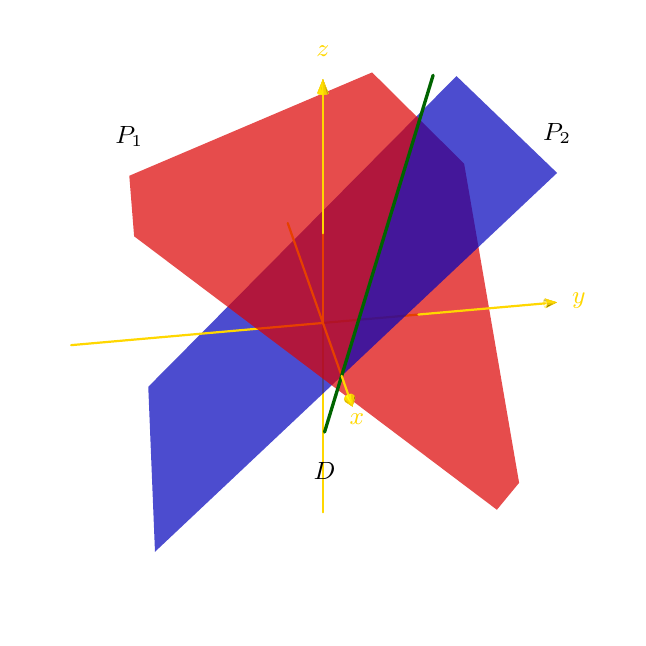
\begin{tikzpicture}%
\pgfsetxvec{\pgfxy(0.625,0)}%
\pgfsetyvec{\pgfxy(0,0.625)}%
\useasboundingbox (-6,-6)--(6,6);
%image  (User)
\pgfsetstrokecolor{rgb,1:red,1;green,0.8431;blue,0}%
\pgfsetlinewidth{0.8pt}%
\pgfsetroundcap%
\pgfsetroundjoin%
\pgfxyline(1.9404,0.1711)(0,0)%
\pgfxyline(0,-3.849)(0,0)%
\pgfsetstrokecolor{rgb,1:red,0;green,0;blue,0}%
\pgfsetlinewidth{0.3pt}%
\pgfputat{\pgfxy(0.0324,-3.018)}{\pgftext{\color{rgb,1:red,0;green,0;blue,0}\small $D$}}\pgfstroke%
\pgfsetstrokecolor{rgb,1:red,0;green,0;blue,0.7333}%
\pgfsetlinewidth{0.2pt}%
\pgfsetstrokeopacity{0.7}%
\pgfsetfillopacity{0.7}%
\pgfpathmoveto{\pgfxy(0.3797,-1.0766)}%
\pgfpathlineto{\pgfxy(-3.4131,-4.6498)}\pgfpathlineto{\pgfxy(-3.5495,-1.2973)}\pgfpathlineto{\pgfxy(2.0211,4.3181)}\pgfclosepath%
\pgfsetfillcolor{rgb,1:red,0;green,0;blue,0.7333}%
\pgffill%
\pgfsetstrokecolor{rgb,1:red,1;green,0.8431;blue,0}%
\pgfsetlinewidth{0.8pt}%
\pgfsetstrokeopacity{1}%
\pgfxyline(-5.1164,-0.4511)(0,0)%
\pgfxyline(-0.7157,2.0293)(0.3797,-1.0766)%
\pgfxyline(0.0000,1.8232)(0,0)%
\pgfsetstrokecolor{rgb,1:red,0;green,0;blue,0}%
\pgfsetlinewidth{0.3pt}%
\pgfputat{\pgfxy(-3.9351,3.7907)}{\pgftext{\pgfsetfillopacity{1}\color{rgb,1:red,0;green,0;blue,0}\small $P_1$}}\pgfstroke%
\pgfsetstrokecolor{rgb,1:red,0.8627;green,0;blue,0}%
\pgfsetlinewidth{0.2pt}%
\pgfsetstrokeopacity{0.7}%
\pgfpathmoveto{\pgfxy(0.9992,5.0906)}%
\pgfpathlineto{\pgfxy(2.8686,3.2361)}\pgfpathlineto{\pgfxy(3.986,-3.2483)}\pgfpathlineto{\pgfxy(3.5348,-3.7961)}\pgfpathlineto{\pgfxy(-3.837,1.7612)}%
\pgfpathlineto{\pgfxy(-3.9351,2.9907)}\pgfclosepath%
\pgfsetfillcolor{rgb,1:red,0.8627;green,0;blue,0}%
\pgffill%
\pgfsetstrokecolor{rgb,1:red,1;green,0.8431;blue,0}%
\pgfsetlinewidth{0.3pt}%
\pgfsetstrokeopacity{1}%
\pgfputat{\pgfxy(5.2013,0.4586)}{\pgftext{\pgfsetfillopacity{1}\color{rgb,1:red,1;green,0.8431;blue,0}\small $y$}}\pgfstroke%
\pgfsetstrokecolor{rgb,1:red,0;green,0;blue,0}%
\pgfputat{\pgfxy(4.758,3.8482)}{\pgftext{\pgfsetfillopacity{1}\color{rgb,1:red,0;green,0;blue,0}\small $P_2$}}\pgfstroke%
\pgfsetstrokecolor{rgb,1:red,0.9961;green,0.9176;blue,0.498}%
\pgfsetlinewidth{0.1pt}%
\pgfsetfillopacity{1}%
\pgfpathmoveto{\pgfxy(4.4944,0.4849)}%
\pgfpathlineto{\pgfxy(4.516,0.4929)}\pgfpathlineto{\pgfxy(4.7456,0.4184)}\pgfclosepath%
\pgfsetfillcolor{rgb,1:red,0.6863;green,0.6314;blue,0.3451}%
\pgffillstroke%
\pgfpathmoveto{\pgfxy(4.4953,0.3322)}%
\pgfpathlineto{\pgfxy(4.4817,0.3857)}\pgfpathlineto{\pgfxy(4.7456,0.4184)}\pgfclosepath%
\pgfsetfillcolor{rgb,1:red,1;green,1;blue,0.898}%
\pgffillstroke%
\pgfpathmoveto{\pgfxy(4.4817,0.3857)}%
\pgfpathlineto{\pgfxy(4.4813,0.4439)}\pgfpathlineto{\pgfxy(4.7456,0.4184)}\pgfclosepath%
\pgfsetfillcolor{rgb,1:red,1;green,0.9686;blue,0.5255}%
\pgffillstroke%
\pgfpathmoveto{\pgfxy(4.4813,0.4439)}%
\pgfpathlineto{\pgfxy(4.4944,0.4849)}\pgfpathlineto{\pgfxy(4.7456,0.4184)}\pgfclosepath%
\pgfsetfillcolor{rgb,1:red,0.7804;green,0.7176;blue,0.3922}%
\pgffillstroke%
\pgfpathmoveto{\pgfxy(4.5171,0.3037)}%
\pgfpathlineto{\pgfxy(4.4953,0.3322)}\pgfpathlineto{\pgfxy(4.7456,0.4184)}\pgfclosepath%
\pgfsetfillcolor{rgb,1:red,1;green,1;blue,0.549}%
\pgffillstroke%
\pgfpathmoveto{\pgfxy(4.5388,0.3112)}%
\pgfpathlineto{\pgfxy(4.5171,0.3037)}\pgfpathlineto{\pgfxy(4.7456,0.4184)}\pgfclosepath%
\pgfsetfillcolor{rgb,1:red,0.8902;green,0.8196;blue,0.4471}%
\pgffillstroke%
\pgfsetstrokecolor{rgb,1:red,1;green,0.8431;blue,0}%
\pgfsetlinewidth{0.8pt}%
\pgfxyline(4.5165,0.3982)(1.9404,0.1711)%
\pgfsetlinewidth{0.1pt}%
\pgfpathmoveto{\pgfxy(4.5517,0.4108)}%
\pgfpathlineto{\pgfxy(4.552,0.3521)}\pgfpathlineto{\pgfxy(4.7456,0.4184)}\pgfclosepath%
\pgfsetfillcolor{rgb,1:red,0.9176;green,0.7725;blue,0}%
\pgffillstroke%
\pgfpathmoveto{\pgfxy(4.5379,0.4647)}%
\pgfpathlineto{\pgfxy(4.5517,0.4108)}\pgfpathlineto{\pgfxy(4.7456,0.4184)}\pgfclosepath%
\pgfsetfillcolor{rgb,1:red,1;green,0.8706;blue,0}%
\pgffillstroke%
\pgfpathmoveto{\pgfxy(4.516,0.4929)}%
\pgfpathlineto{\pgfxy(4.5379,0.4647)}\pgfpathlineto{\pgfxy(4.7456,0.4184)}\pgfclosepath%
\pgfsetfillcolor{rgb,1:red,0.9725;green,0.8196;blue,0}%
\pgffillstroke%
\pgfpathmoveto{\pgfxy(4.552,0.3521)}%
\pgfpathlineto{\pgfxy(4.5388,0.3112)}\pgfpathlineto{\pgfxy(4.7456,0.4184)}\pgfclosepath%
\pgfsetfillcolor{rgb,1:red,0.4627;green,0.3882;blue,0}%
\pgffillstroke%
\pgfsetlinewidth{0.3pt}%
\pgfputat{\pgfxy(0.6905,-1.9581)}{\pgftext{\color{rgb,1:red,1;green,0.8431;blue,0}\small $x$}}\pgfstroke%
\pgfsetstrokecolor{rgb,1:red,0.9961;green,0.9176;blue,0.498}%
\pgfsetlinewidth{0.1pt}%
\pgfpathmoveto{\pgfxy(0.5738,-1.6195)}%
\pgfpathlineto{\pgfxy(0.6297,-1.58)}\pgfpathlineto{\pgfxy(0.5974,-1.6939)}\pgfclosepath%
\pgfsetfillcolor{rgb,1:red,0.9843;green,0.9059;blue,0.4902}%
\pgffillstroke%
\pgfpathmoveto{\pgfxy(0.5053,-1.6264)}%
\pgfpathlineto{\pgfxy(0.5738,-1.6195)}\pgfpathlineto{\pgfxy(0.5974,-1.6939)}\pgfclosepath%
\pgfsetfillcolor{rgb,1:red,0.949;green,0.8745;blue,0.4745}%
\pgffillstroke%
\pgfpathmoveto{\pgfxy(0.4644,-1.6053)}%
\pgfpathlineto{\pgfxy(0.5053,-1.6264)}\pgfpathlineto{\pgfxy(0.5974,-1.6939)}\pgfclosepath%
\pgfsetfillcolor{rgb,1:red,0.7059;green,0.651;blue,0.3529}%
\pgffillstroke%
\pgfpathmoveto{\pgfxy(0.6297,-1.58)}%
\pgfpathlineto{\pgfxy(0.652,-1.5229)}\pgfpathlineto{\pgfxy(0.5974,-1.6939)}\pgfclosepath%
\pgfsetfillcolor{rgb,1:red,0.8353;green,0.7725;blue,0.4196}%
\pgffillstroke%
\pgfsetstrokecolor{rgb,1:red,1;green,0.8431;blue,0}%
\pgfpathmoveto{\pgfxy(0.652,-1.5229)}%
\pgfpathlineto{\pgfxy(0.6318,-1.4698)}\pgfpathlineto{\pgfxy(0.5974,-1.6939)}\pgfclosepath%
\pgfsetfillcolor{rgb,1:red,0.4902;green,0.4118;blue,0}%
\pgffillstroke%
\pgfpathmoveto{\pgfxy(0.6318,-1.4698)}%
\pgfpathlineto{\pgfxy(0.6178,-1.4625)}\pgfpathlineto{\pgfxy(0.5974,-1.6939)}\pgfclosepath%
\pgfsetfillcolor{rgb,1:red,0.9451;green,0.8;blue,0}%
\pgffillstroke%
\pgfsetstrokecolor{rgb,1:red,0;green,0;blue,0.7333}%
\pgfsetlinewidth{0.2pt}%
\pgfsetstrokeopacity{0.7}%
\pgfsetfillopacity{0.7}%
\pgfpathmoveto{\pgfxy(2.7135,5.016)}%
\pgfpathlineto{\pgfxy(4.758,3.0482)}\pgfpathlineto{\pgfxy(0.3797,-1.0766)}\pgfpathlineto{\pgfxy(2.0211,4.3181)}\pgfclosepath%
\pgfsetfillcolor{rgb,1:red,0;green,0;blue,0.7333}%
\pgffill%
\pgfsetstrokecolor{rgb,1:red,0;green,0.3922;blue,0}%
\pgfsetlinewidth{1.2pt}%
\pgfsetstrokeopacity{1}%
\pgfxyline(0.252,-1.4963)(0.2602,-1.4693)%
\pgfsetstrokecolor{rgb,1:red,0.9961;green,0.9176;blue,0.498}%
\pgfsetlinewidth{0.1pt}%
\pgfsetfillopacity{1}%
\pgfpathmoveto{\pgfxy(0.4503,-1.5981)}%
\pgfpathlineto{\pgfxy(0.4644,-1.6053)}\pgfpathlineto{\pgfxy(0.5974,-1.6939)}\pgfclosepath%
\pgfsetfillcolor{rgb,1:red,0.7059;green,0.651;blue,0.3529}%
\pgffillstroke%
\pgfsetstrokecolor{rgb,1:red,0;green,0.3922;blue,0}%
\pgfsetlinewidth{1.2pt}%
\pgfxyline(0.2602,-1.4693)(0.7628,0.1824)%
\pgfsetstrokecolor{rgb,1:red,1;green,0.8431;blue,0}%
\pgfsetlinewidth{0.8pt}%
\pgfxyline(0.541,-1.534)(0.3797,-1.0766)%
\pgfsetlinewidth{0.1pt}%
\pgfpathmoveto{\pgfxy(0.5768,-1.4412)}%
\pgfpathlineto{\pgfxy(0.508,-1.448)}\pgfpathlineto{\pgfxy(0.5974,-1.6939)}\pgfclosepath%
\pgfsetfillcolor{rgb,1:red,1;green,0.9412;blue,0}%
\pgffillstroke%
\pgfpathmoveto{\pgfxy(0.508,-1.448)}%
\pgfpathlineto{\pgfxy(0.4518,-1.4878)}\pgfpathlineto{\pgfxy(0.5974,-1.6939)}\pgfclosepath%
\pgfsetfillcolor{rgb,1:red,1;green,1;blue,0.0471}%
\pgffillstroke%
\pgfpathmoveto{\pgfxy(0.4518,-1.4878)}%
\pgfpathlineto{\pgfxy(0.4298,-1.5452)}\pgfpathlineto{\pgfxy(0.5974,-1.6939)}\pgfclosepath%
\pgfsetfillcolor{rgb,1:red,1;green,0.8706;blue,0}%
\pgffillstroke%
\pgfpathmoveto{\pgfxy(0.6178,-1.4625)}%
\pgfpathlineto{\pgfxy(0.5768,-1.4412)}\pgfpathlineto{\pgfxy(0.5974,-1.6939)}\pgfclosepath%
\pgfsetfillcolor{rgb,1:red,0.9451;green,0.8;blue,0}%
\pgffillstroke%
\pgfsetstrokecolor{rgb,1:red,0;green,0.3922;blue,0}%
\pgfsetlinewidth{1.2pt}%
\pgfxyline(2.2383,5.032)(1.2158,1.6715)%
\pgfsetstrokecolor{rgb,1:red,1;green,0.8431;blue,0}%
\pgfsetlinewidth{0.3pt}%
\pgfputat{\pgfxy(0,5.5225)}{\pgftext{\color{rgb,1:red,1;green,0.8431;blue,0}\small $z$}}\pgfstroke%
\pgfsetstrokecolor{rgb,1:red,0.9961;green,0.9176;blue,0.498}%
\pgfsetlinewidth{0.1pt}%
\pgfpathmoveto{\pgfxy(0.1124,4.6632)}%
\pgfpathlineto{\pgfxy(0.1,4.6838)}\pgfpathlineto{\pgfxy(0.0000,4.9487)}\pgfclosepath%
\pgfsetfillcolor{rgb,1:red,0.4824;green,0.4431;blue,0.2392}%
\pgffillstroke%
\pgfpathmoveto{\pgfxy(-0.0196,4.7011)}%
\pgfpathlineto{\pgfxy(-0.0813,4.6913)}\pgfpathlineto{\pgfxy(0.0000,4.9487)}\pgfclosepath%
\pgfsetfillcolor{rgb,1:red,0.3804;green,0.349;blue,0.1922}%
\pgffillstroke%
\pgfpathmoveto{\pgfxy(0.0495,4.6982)}%
\pgfpathlineto{\pgfxy(-0.0196,4.7011)}\pgfpathlineto{\pgfxy(0.0000,4.9487)}\pgfclosepath%
\pgfsetfillcolor{rgb,1:red,0.7137;green,0.6588;blue,0.3569}%
\pgffillstroke%
\pgfsetstrokecolor{rgb,1:red,0;green,0.3922;blue,0}%
\pgfsetlinewidth{1.2pt}%
\pgfxyline(1.2158,1.6715)(1.1735,1.5322)%
\pgfsetstrokecolor{rgb,1:red,0.9961;green,0.9176;blue,0.498}%
\pgfsetlinewidth{0.1pt}%
\pgfpathmoveto{\pgfxy(0.1,4.6838)}%
\pgfpathlineto{\pgfxy(0.0495,4.6982)}\pgfpathlineto{\pgfxy(0.0000,4.9487)}\pgfclosepath%
\pgfsetfillcolor{rgb,1:red,0.7255;green,0.6706;blue,0.3647}%
\pgffillstroke%
\pgfpathmoveto{\pgfxy(-0.0813,4.6913)}%
\pgfpathlineto{\pgfxy(-0.1123,4.6726)}\pgfpathlineto{\pgfxy(0.0000,4.9487)}\pgfclosepath%
\pgfsetfillcolor{rgb,1:red,0.7725;green,0.7098;blue,0.3843}%
\pgffillstroke%
\pgfsetstrokecolor{rgb,1:red,1;green,0.8431;blue,0}%
\pgfsetlinewidth{0.8pt}%
\pgfxyline(-0.0000,4.6679)(0.0000,1.8232)%
\pgfsetstrokecolor{rgb,1:red,0;green,0.3922;blue,0}%
\pgfsetlinewidth{1.2pt}%
\pgfxyline(0.7628,0.1824)(1.1735,1.5322)%
\pgfsetstrokecolor{rgb,1:red,1;green,0.8431;blue,0}%
\pgfsetlinewidth{0.1pt}%
\pgfpathmoveto{\pgfxy(-0.05,4.6374)}%
\pgfpathlineto{\pgfxy(0.0198,4.6345)}\pgfpathlineto{\pgfxy(0.0000,4.9487)}\pgfclosepath%
\pgfsetfillcolor{rgb,1:red,1;green,0.902;blue,0}%
\pgffillstroke%
\pgfpathmoveto{\pgfxy(0.0198,4.6345)}%
\pgfpathlineto{\pgfxy(0.0819,4.6444)}\pgfpathlineto{\pgfxy(0.0000,4.9487)}\pgfclosepath%
\pgfsetfillcolor{rgb,1:red,0.9608;green,0.8118;blue,0}%
\pgffillstroke%
\pgfpathmoveto{\pgfxy(0.0819,4.6444)}%
\pgfpathlineto{\pgfxy(0.1124,4.6632)}\pgfpathlineto{\pgfxy(0.0000,4.9487)}\pgfclosepath%
\pgfsetfillcolor{rgb,1:red,0.7333;green,0.6196;blue,0}%
\pgffillstroke%
\pgfpathmoveto{\pgfxy(-0.1123,4.6726)}%
\pgfpathlineto{\pgfxy(-0.1004,4.652)}\pgfpathlineto{\pgfxy(0.0000,4.9487)}\pgfclosepath%
\pgfsetfillcolor{rgb,1:red,0.9843;green,0.8275;blue,0}%
\pgffillstroke%
\pgfpathmoveto{\pgfxy(-0.1004,4.652)}%
\pgfpathlineto{\pgfxy(-0.05,4.6374)}\pgfpathlineto{\pgfxy(0.0000,4.9487)}\pgfclosepath%
\pgfsetfillcolor{rgb,1:red,1;green,0.9059;blue,0}%
\pgffillstroke%
\pgfpathmoveto{\pgfxy(0.4298,-1.5452)}%
\pgfpathlineto{\pgfxy(0.4503,-1.5981)}\pgfpathlineto{\pgfxy(0.5974,-1.6939)}\pgfclosepath%
\pgfsetfillcolor{rgb,1:red,0.7412;green,0.6235;blue,0}%
\pgffillstroke%
\pgfsetstrokecolor{rgb,1:red,0;green,0.3922;blue,0}%
\pgfsetlinewidth{1.2pt}%
\pgfxyline(0.0324,-2.218)(0.252,-1.4963)%
\end{tikzpicture}%
\egroup%
&$\quad$&% TeXgraph version 1.92
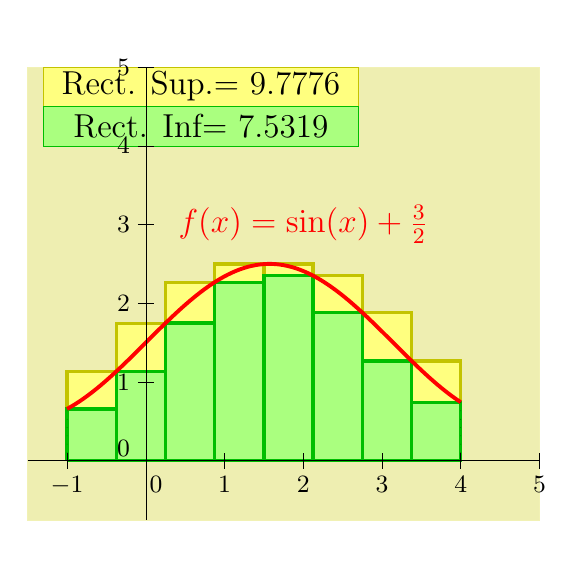
\begin{tikzpicture}%
\pgfsetxvec{\pgfxy(1,0)}%
\pgfsetyvec{\pgfxy(0,1)}%
\useasboundingbox (-1.5,-1.25)--(5,5.5);
%\begin{pgfpicture}{-1.5cm}{-1.25cm}{5cm}{5.5cm}%
%\pgfsetroundjoin%
%fond  (Utilisateur)
\pgfsetstrokecolor{rgb,1:red,0.9451;green,0.9451;blue,0.7059}\pgfsetlinewidth{0.2pt} 
\pgfmoveto{\pgfxy(-1.5,-0.75)}\pgflineto{\pgfxy(5,-0.75)}\pgflineto{\pgfxy(5,5)}
\pgflineto{\pgfxy(-1.5,5)}\pgfclosepath
\pgfsetfillcolor{rgb,1:red,0.9333;green,0.9333;blue,0.6941}
\pgffillstroke
%MetRectSup  (Utilisateur)
\pgfsetstrokecolor{rgb,1:red,0.7647;green,0.7647;blue,0}\pgfsetlinewidth{1.2pt} 
\pgfmoveto{\pgfxy(-1,0)}\pgflineto{\pgfxy(-1,1.1328)}\pgflineto{\pgfxy(-0.375,1.1328)}
\pgflineto{\pgfxy(-0.375,0)}\pgflineto{\pgfxy(-1,0)}
\pgfsetfillcolor{rgb,1:red,1;green,1;blue,0.498}
\pgffillstroke
\pgfmoveto{\pgfxy(-0.375,0)}
\pgflineto{\pgfxy(-0.375,1.7464)}\pgflineto{\pgfxy(0.25,1.7464)}\pgflineto{\pgfxy(0.25,0)}
\pgflineto{\pgfxy(-0.375,0)}
\pgffillstroke
\pgfmoveto{\pgfxy(0.25,0)}\pgflineto{\pgfxy(0.25,2.2669)}
\pgflineto{\pgfxy(0.875,2.2669)}\pgflineto{\pgfxy(0.875,0)}\pgflineto{\pgfxy(0.25,0)}
\pgffillstroke
\pgfmoveto{\pgfxy(0.875,0)}\pgflineto{\pgfxy(0.875,2.4975)}\pgflineto{\pgfxy(1.5,2.4975)}
\pgflineto{\pgfxy(1.5,0)}\pgflineto{\pgfxy(0.875,0)}
\pgffillstroke
\pgfmoveto{\pgfxy(1.5,0)}
\pgflineto{\pgfxy(1.5,2.5)}\pgflineto{\pgfxy(2.125,2.5)}\pgflineto{\pgfxy(2.125,0)}
\pgflineto{\pgfxy(1.5,0)}
\pgffillstroke
\pgfmoveto{\pgfxy(2.125,0)}\pgflineto{\pgfxy(2.125,2.3503)}
\pgflineto{\pgfxy(2.75,2.3503)}\pgflineto{\pgfxy(2.75,0)}\pgflineto{\pgfxy(2.125,0)}
\pgffillstroke
\pgfmoveto{\pgfxy(2.75,0)}\pgflineto{\pgfxy(2.75,1.8817)}\pgflineto{\pgfxy(3.375,1.8817)}
\pgflineto{\pgfxy(3.375,0)}\pgflineto{\pgfxy(2.75,0)}
\pgffillstroke
\pgfmoveto{\pgfxy(3.375,0)}
\pgflineto{\pgfxy(3.375,1.2687)}\pgflineto{\pgfxy(4,1.2687)}\pgflineto{\pgfxy(4,0)}
\pgflineto{\pgfxy(3.375,0)}
\pgffillstroke
\pgfsetlinewidth{0.2pt} 
\pgfmoveto{\pgfxy(-1.3,4.5)}\pgflineto{\pgfxy(2.7,4.5)}\pgflineto{\pgfxy(2.7,5)}
\pgflineto{\pgfxy(-1.3,5)}\pgfclosepath
\pgffillstroke
\pgfsetstrokecolor{black}
\pgfputat{\pgfxy(0.7,4.75)}{\pgftext{\color{black}\large Rect. Sup.= 9.7776}}
%MetRectInf  (Utilisateur)
\pgfsetstrokecolor{rgb,1:red,0;green,0.7451;blue,0}\pgfsetlinewidth{1.2pt} 
\pgfmoveto{\pgfxy(-1,0)}\pgflineto{\pgfxy(-1,0.6585)}\pgflineto{\pgfxy(-0.375,0.6585)}
\pgflineto{\pgfxy(-0.375,0)}\pgflineto{\pgfxy(-1,0)}
\pgfsetfillcolor{rgb,1:red,0.6667;green,1;blue,0.498}
\pgffillstroke
\pgfmoveto{\pgfxy(-0.375,0)}
\pgflineto{\pgfxy(-0.375,1.1337)}\pgflineto{\pgfxy(0.25,1.1337)}\pgflineto{\pgfxy(0.25,0)}
\pgflineto{\pgfxy(-0.375,0)}
\pgffillstroke
\pgfmoveto{\pgfxy(0.25,0)}\pgflineto{\pgfxy(0.25,1.7474)}
\pgflineto{\pgfxy(0.875,1.7474)}\pgflineto{\pgfxy(0.875,0)}\pgflineto{\pgfxy(0.25,0)}
\pgffillstroke
\pgfmoveto{\pgfxy(0.875,0)}\pgflineto{\pgfxy(0.875,2.2675)}\pgflineto{\pgfxy(1.5,2.2675)}
\pgflineto{\pgfxy(1.5,0)}\pgflineto{\pgfxy(0.875,0)}
\pgffillstroke
\pgfmoveto{\pgfxy(1.5,0)}
\pgflineto{\pgfxy(1.5,2.3503)}\pgflineto{\pgfxy(2.125,2.3503)}\pgflineto{\pgfxy(2.125,0)}
\pgflineto{\pgfxy(1.5,0)}
\pgffillstroke
\pgfmoveto{\pgfxy(2.125,0)}\pgflineto{\pgfxy(2.125,1.8817)}
\pgflineto{\pgfxy(2.75,1.8817)}\pgflineto{\pgfxy(2.75,0)}\pgflineto{\pgfxy(2.125,0)}
\pgffillstroke
\pgfmoveto{\pgfxy(2.75,0)}\pgflineto{\pgfxy(2.75,1.2687)}\pgflineto{\pgfxy(3.375,1.2687)}
\pgflineto{\pgfxy(3.375,0)}\pgflineto{\pgfxy(2.75,0)}
\pgffillstroke
\pgfmoveto{\pgfxy(3.375,0)}
\pgflineto{\pgfxy(3.375,0.7432)}\pgflineto{\pgfxy(4,0.7432)}\pgflineto{\pgfxy(4,0)}
\pgflineto{\pgfxy(3.375,0)}
\pgffillstroke
\pgfsetlinewidth{0.2pt} 
\pgfmoveto{\pgfxy(-1.3,4)}\pgflineto{\pgfxy(2.7,4)}\pgflineto{\pgfxy(2.7,4.5)}
\pgflineto{\pgfxy(-1.3,4.5)}\pgfclosepath
\pgffillstroke
\pgfsetstrokecolor{black}
\pgfputat{\pgfxy(0.7,4.25)}{\pgftext{\color{black}\large Rect. Inf= 7.5319}}
%RiemGauche  (Utilisateur)
%RiemDroite  (Utilisateur)
%MethSimp  (Utilisateur)
%Methtrap  (Utilisateur)
%MetRecMed  (Utilisateur)
%EscSup  (Utilisateur)
%EscInf  (Utilisateur)
%courbe  (Utilisateur)
\pgfsetstrokecolor{rgb,1:red,1;green,0;blue,0}\pgfsetlinewidth{1.4pt} 
\pgfmoveto{\pgfxy(-1,0.6585)}\pgflineto{\pgfxy(-0.949,0.6872)}\pgflineto{\pgfxy(-0.898,0.7179)}
\pgflineto{\pgfxy(-0.8469,0.7507)}\pgflineto{\pgfxy(-0.7959,0.7855)}\pgflineto{\pgfxy(-0.7449,0.8221)}
\pgflineto{\pgfxy(-0.6939,0.8605)}\pgflineto{\pgfxy(-0.6429,0.9005)}\pgflineto{\pgfxy(-0.5918,0.9421)}
\pgflineto{\pgfxy(-0.5408,0.9852)}\pgflineto{\pgfxy(-0.4898,1.0296)}\pgflineto{\pgfxy(-0.4388,1.0752)}
\pgflineto{\pgfxy(-0.3878,1.1219)}\pgflineto{\pgfxy(-0.3367,1.1696)}\pgflineto{\pgfxy(-0.2857,1.2182)}
\pgflineto{\pgfxy(-0.2347,1.2675)}\pgflineto{\pgfxy(-0.1837,1.3174)}\pgflineto{\pgfxy(-0.1327,1.3677)}
\pgflineto{\pgfxy(-0.0816,1.4185)}\pgflineto{\pgfxy(-0.0306,1.4694)}\pgflineto{\pgfxy(0.0204,1.5204)}
\pgflineto{\pgfxy(0.0714,1.5714)}\pgflineto{\pgfxy(0.1224,1.6221)}\pgflineto{\pgfxy(0.1735,1.6726)}
\pgflineto{\pgfxy(0.2245,1.7226)}\pgflineto{\pgfxy(0.2755,1.772)}\pgflineto{\pgfxy(0.3265,1.8208)}
\pgflineto{\pgfxy(0.3776,1.8686)}\pgflineto{\pgfxy(0.4286,1.9156)}\pgflineto{\pgfxy(0.4796,1.9614)}
\pgflineto{\pgfxy(0.5306,2.0061)}\pgflineto{\pgfxy(0.5816,2.0494)}\pgflineto{\pgfxy(0.6327,2.0913)}
\pgflineto{\pgfxy(0.6837,2.1316)}\pgflineto{\pgfxy(0.7347,2.1704)}\pgflineto{\pgfxy(0.7857,2.2073)}
\pgflineto{\pgfxy(0.8367,2.2425)}\pgflineto{\pgfxy(0.8878,2.2757)}\pgflineto{\pgfxy(0.9388,2.3068)}
\pgflineto{\pgfxy(0.9898,2.3359)}\pgflineto{\pgfxy(1.0408,2.3628)}\pgflineto{\pgfxy(1.0918,2.3875)}
\pgflineto{\pgfxy(1.1429,2.4098)}\pgflineto{\pgfxy(1.1939,2.4298)}\pgflineto{\pgfxy(1.2449,2.4474)}
\pgflineto{\pgfxy(1.2959,2.4625)}\pgflineto{\pgfxy(1.3469,2.475)}\pgflineto{\pgfxy(1.398,2.4851)}
\pgflineto{\pgfxy(1.449,2.4926)}\pgflineto{\pgfxy(1.5,2.4975)}\pgflineto{\pgfxy(1.551,2.4998)}
\pgflineto{\pgfxy(1.602,2.4995)}\pgflineto{\pgfxy(1.6531,2.4966)}\pgflineto{\pgfxy(1.7041,2.4911)}
\pgflineto{\pgfxy(1.7551,2.4831)}\pgflineto{\pgfxy(1.8061,2.4724)}\pgflineto{\pgfxy(1.8571,2.4593)}
\pgflineto{\pgfxy(1.9082,2.4436)}\pgflineto{\pgfxy(1.9592,2.4255)}\pgflineto{\pgfxy(2.0102,2.405)}
\pgflineto{\pgfxy(2.0612,2.3821)}\pgflineto{\pgfxy(2.1122,2.357)}\pgflineto{\pgfxy(2.1633,2.3296)}
\pgflineto{\pgfxy(2.2143,2.3)}\pgflineto{\pgfxy(2.2653,2.2684)}\pgflineto{\pgfxy(2.3163,2.2347)}
\pgflineto{\pgfxy(2.3673,2.1992)}\pgflineto{\pgfxy(2.4184,2.1618)}\pgflineto{\pgfxy(2.4694,2.1227)}
\pgflineto{\pgfxy(2.5204,2.082)}\pgflineto{\pgfxy(2.5714,2.0398)}\pgflineto{\pgfxy(2.6224,1.9961)}
\pgflineto{\pgfxy(2.6735,1.9512)}\pgflineto{\pgfxy(2.7245,1.9051)}\pgflineto{\pgfxy(2.7755,1.858)}
\pgflineto{\pgfxy(2.8265,1.8099)}\pgflineto{\pgfxy(2.8776,1.761)}\pgflineto{\pgfxy(2.9286,1.7114)}
\pgflineto{\pgfxy(2.9796,1.6613)}\pgflineto{\pgfxy(3.0306,1.6108)}\pgflineto{\pgfxy(3.0816,1.5599)}
\pgflineto{\pgfxy(3.1327,1.5089)}\pgflineto{\pgfxy(3.1837,1.4579)}\pgflineto{\pgfxy(3.2347,1.407)}
\pgflineto{\pgfxy(3.2857,1.3564)}\pgflineto{\pgfxy(3.3367,1.3061)}\pgflineto{\pgfxy(3.3878,1.2563)}
\pgflineto{\pgfxy(3.4388,1.2072)}\pgflineto{\pgfxy(3.4898,1.1588)}\pgflineto{\pgfxy(3.5408,1.1113)}
\pgflineto{\pgfxy(3.5918,1.0648)}\pgflineto{\pgfxy(3.6429,1.0195)}\pgflineto{\pgfxy(3.6939,0.9754)}
\pgflineto{\pgfxy(3.7449,0.9326)}\pgflineto{\pgfxy(3.7959,0.8914)}\pgflineto{\pgfxy(3.8469,0.8517)}
\pgflineto{\pgfxy(3.898,0.8137)}\pgflineto{\pgfxy(3.949,0.7775)}\pgflineto{\pgfxy(4,0.7432)}
\pgfstroke
\pgfsetstrokecolor{black}\pgfsetlinewidth{0.2pt} 
\pgfsetroundcap \pgfsetdash{{0pt}{3pt}}{0pt}
\pgfxyline(-1,0)(-1,0.6585)\pgfxyline(4,0)(4,0.7432)
\pgfsetbuttcap%
%label  (Utilisateur)
\pgfsetdash{}{0pt}
\pgfsetstrokecolor{rgb,1:red,1;green,0;blue,0}
\pgfputat{\pgfxy(2,3)}{\pgftext{\color{rgb,1:red,1;green,0;blue,0}\large $f(x)=\sin(x)+\frac32$}}
%axes1  (Axes)
\pgfsetstrokecolor{black}
\pgfxyline(-1.5,0)(5,0)\pgfxyline(0,-0.75)(0,5)
\pgfsetfillcolor{black}
\pgfxyline(0,-0.1)(0,0.1)\pgfxyline(1,-0.1)(1,0.1)\pgfxyline(2,-0.1)(2,0.1)\pgfxyline(3,-0.1)(3,0.1)
\pgfxyline(4,-0.1)(4,0.1)\pgfxyline(5,-0.1)(5,0.1)
\pgfputat{\pgfxy(0.05,-0.2)}{\pgftext[top,left]{\small $0$}}
\pgfputat{\pgfxy(1,-0.2)}{\pgftext[top]{\small $1$}}
\pgfputat{\pgfxy(2,-0.2)}{\pgftext[top]{\small $2$}}
\pgfputat{\pgfxy(3,-0.2)}{\pgftext[top]{\small $3$}}
\pgfputat{\pgfxy(4,-0.2)}{\pgftext[top]{\small $4$}}
\pgfputat{\pgfxy(5,-0.2)}{\pgftext[top]{\small $5$}}
\pgfxyline(-1,-0.1)(-1,0.1)
\pgfputat{\pgfxy(-1,-0.2)}{\pgftext[top]{\small $-1$}}
\pgfxyline(-0.1,0)(0.1,0)\pgfxyline(-0.1,1)(0.1,1)\pgfxyline(-0.1,2)(0.1,2)\pgfxyline(-0.1,3)(0.1,3)
\pgfxyline(-0.1,4)(0.1,4)\pgfxyline(-0.1,5)(0.1,5)
\pgfputat{\pgfxy(-0.2,0.05)}{\pgftext[right,bottom]{\small $0$}}
\pgfputat{\pgfxy(-0.2,1)}{\pgftext[right]{\small $1$}}
\pgfputat{\pgfxy(-0.2,2)}{\pgftext[right]{\small $2$}}
\pgfputat{\pgfxy(-0.2,3)}{\pgftext[right]{\small $3$}}
\pgfputat{\pgfxy(-0.2,4)}{\pgftext[right]{\small $4$}}
\pgfputat{\pgfxy(-0.2,5)}{\pgftext[right]{\small $5$}}
\end{tikzpicture}%
\\
\\
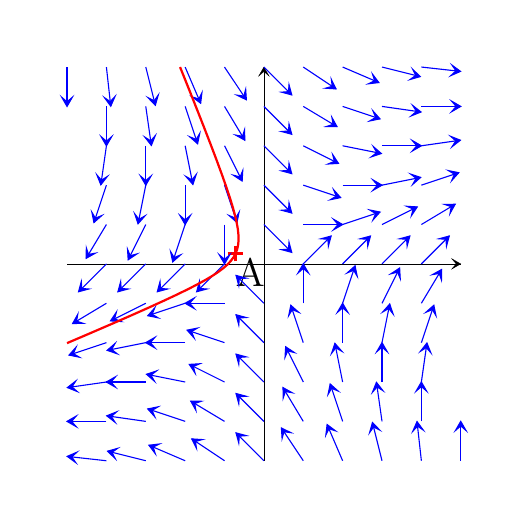
\begin{tikzpicture}%
\pgfsetxvec{\pgfxy(1,0)}%
\pgfsetyvec{\pgfxy(0,1)}%
\useasboundingbox (-3,-3)--(3,3);
%\begin{pgfpicture}{-3cm}{-3cm}{3cm}{3cm}
%\pgfsetroundjoin
%  (Axes)
\pgfsetlinewidth{0.1pt} 
\pgfsetfillcolor{black}
\pgfmoveto{\pgfxy(2.3845,0.0667)}\pgflineto{\pgfxy(2.5,0)}\pgflineto{\pgfxy(2.3845,-0.0667)}\pgflineto{\pgfxy(2.4423,0)}\pgfclosepath\pgffillstroke
\pgfmoveto{\pgfxy(-0.0667,2.3845)}\pgflineto{\pgfxy(0,2.5)}\pgflineto{\pgfxy(0.0667,2.3845)}\pgflineto{\pgfxy(0,2.4423)}\pgfclosepath\pgffillstroke
\pgfxyline(-2.5,0)(2.5,0)\pgfxyline(0,-2.5)(0,2.5)
%PointA  (Point(s))
\pgfsetstrokecolor{rgb,1:red,1;green,0;blue,0}\pgfsetlinewidth{0.8pt} 
\pgfmoveto{\pgfxy(-0.4597,0.1316)}\pgflineto{\pgfxy(-0.2597,0.1316)}\pgfstroke
\pgfmoveto{\pgfxy(-0.3597,0.0316)}\pgflineto{\pgfxy(-0.3597,0.2316)}\pgfstroke 
%LabelA  (Label)
\pgfputat{\pgfxy(-0.3597,-0.1184)}{\pgftext[left]{\Large A}}
%champ  (Utilisateur)
\pgfsetstrokecolor{rgb,1:red,0;green,0;blue,1}\pgfsetlinewidth{0.4pt} 
\pgfsetfillcolor{rgb,1:red,0;green,0;blue,1}
\pgfmoveto{\pgfxy(-2.3895,-2.5238)}\pgflineto{\pgfxy(-2.4969,-2.4448)}\pgflineto{\pgfxy(-2.3748,-2.3913)}\pgflineto{\pgfxy(-2.4396,-2.4512)}\pgfclosepath\pgffillstroke
\pgfxyline(-2,-2.5)(-2.4969,-2.4448)
\pgfmoveto{\pgfxy(-1.8892,-2.4714)}\pgflineto{\pgfxy(-1.9851,-2.3787)}\pgflineto{\pgfxy(-1.8569,-2.3421)}\pgflineto{\pgfxy(-1.9291,-2.3927)}\pgfclosepath\pgffillstroke
\pgfxyline(-1.5,-2.5)(-1.9851,-2.3787)
\pgfmoveto{\pgfxy(-1.3797,-2.4098)}\pgflineto{\pgfxy(-1.4596,-2.303)}\pgflineto{\pgfxy(-1.3272,-2.2872)}\pgflineto{\pgfxy(-1.4065,-2.3258)}\pgfclosepath\pgffillstroke
\pgfxyline(-1,-2.5)(-1.4596,-2.303)
\pgfmoveto{\pgfxy(-0.8569,-2.3422)}\pgflineto{\pgfxy(-0.916,-2.2226)}\pgflineto{\pgfxy(-0.783,-2.2312)}\pgflineto{\pgfxy(-0.868,-2.2547)}\pgfclosepath\pgffillstroke
\pgfxyline(-0.5,-2.5)(-0.916,-2.2226)
\pgfmoveto{\pgfxy(-0.319,-2.2752)}\pgflineto{\pgfxy(-0.3536,-2.1464)}\pgflineto{\pgfxy(-0.2248,-2.181)}\pgflineto{\pgfxy(-0.3127,-2.1873)}\pgfclosepath\pgffillstroke
\pgfxyline(0,-2.5)(-0.3536,-2.1464)
\pgfmoveto{\pgfxy(0.2312,-2.217)}\pgflineto{\pgfxy(0.2226,-2.084)}\pgflineto{\pgfxy(0.3422,-2.1431)}\pgflineto{\pgfxy(0.2547,-2.132)}\pgfclosepath\pgffillstroke
\pgfxyline(0.5,-2.5)(0.2226,-2.084)
\pgfmoveto{\pgfxy(0.7872,-2.1728)}\pgflineto{\pgfxy(0.803,-2.0404)}\pgflineto{\pgfxy(0.9098,-2.1203)}\pgflineto{\pgfxy(0.8258,-2.0935)}\pgfclosepath\pgffillstroke
\pgfxyline(1,-2.5)(0.803,-2.0404)
\pgfmoveto{\pgfxy(1.3421,-2.1431)}\pgflineto{\pgfxy(1.3787,-2.0149)}\pgflineto{\pgfxy(1.4714,-2.1108)}\pgflineto{\pgfxy(1.3927,-2.0709)}\pgfclosepath\pgffillstroke
\pgfxyline(1.5,-2.5)(1.3787,-2.0149)
\pgfmoveto{\pgfxy(1.8913,-2.1252)}\pgflineto{\pgfxy(1.9448,-2.0031)}\pgflineto{\pgfxy(2.0238,-2.1105)}\pgflineto{\pgfxy(1.9512,-2.0604)}\pgfclosepath\pgffillstroke
\pgfxyline(2,-2.5)(1.9448,-2.0031)
\pgfmoveto{\pgfxy(2.4333,-2.1155)}\pgflineto{\pgfxy(2.5,-2)}\pgflineto{\pgfxy(2.5667,-2.1155)}\pgflineto{\pgfxy(2.5,-2.0577)}\pgfclosepath\pgffillstroke
\pgfxyline(2.5,-2.5)(2.5,-2)
\pgfmoveto{\pgfxy(-2.3845,-2.0667)}\pgflineto{\pgfxy(-2.5,-2)}\pgflineto{\pgfxy(-2.3845,-1.9333)}\pgflineto{\pgfxy(-2.4423,-2)}\pgfclosepath\pgffillstroke
\pgfxyline(-2,-2)(-2.5,-2)
\pgfmoveto{\pgfxy(-1.8901,-2.0116)}\pgflineto{\pgfxy(-1.995,-1.9293)}\pgflineto{\pgfxy(-1.8712,-1.8796)}\pgflineto{\pgfxy(-1.9378,-1.9375)}\pgfclosepath\pgffillstroke
\pgfxyline(-1.5,-2)(-1.995,-1.9293)
\pgfmoveto{\pgfxy(-1.3859,-1.9416)}\pgflineto{\pgfxy(-1.4743,-1.8419)}\pgflineto{\pgfxy(-1.3437,-1.8152)}\pgflineto{\pgfxy(-1.4196,-1.8601)}\pgfclosepath\pgffillstroke
\pgfxyline(-1,-2)(-1.4743,-1.8419)
\pgfmoveto{\pgfxy(-0.864,-1.8593)}\pgflineto{\pgfxy(-0.9287,-1.7428)}\pgflineto{\pgfxy(-0.7954,-1.745)}\pgflineto{\pgfxy(-0.8792,-1.7725)}\pgfclosepath\pgffillstroke
\pgfxyline(-0.5,-2)(-0.9287,-1.7428)
\pgfmoveto{\pgfxy(-0.319,-1.7752)}\pgflineto{\pgfxy(-0.3536,-1.6464)}\pgflineto{\pgfxy(-0.2248,-1.681)}\pgflineto{\pgfxy(-0.3127,-1.6873)}\pgfclosepath\pgffillstroke
\pgfxyline(0,-2)(-0.3536,-1.6464)
\pgfmoveto{\pgfxy(0.245,-1.7046)}\pgflineto{\pgfxy(0.2428,-1.5713)}\pgflineto{\pgfxy(0.3593,-1.636)}\pgflineto{\pgfxy(0.2725,-1.6208)}\pgfclosepath\pgffillstroke
\pgfxyline(0.5,-2)(0.2428,-1.5713)
\pgfmoveto{\pgfxy(0.8152,-1.6563)}\pgflineto{\pgfxy(0.8419,-1.5257)}\pgflineto{\pgfxy(0.9416,-1.6141)}\pgflineto{\pgfxy(0.8601,-1.5804)}\pgfclosepath\pgffillstroke
\pgfxyline(1,-2)(0.8419,-1.5257)
\pgfmoveto{\pgfxy(1.3796,-1.6288)}\pgflineto{\pgfxy(1.4293,-1.505)}\pgflineto{\pgfxy(1.5116,-1.6099)}\pgflineto{\pgfxy(1.4375,-1.5622)}\pgfclosepath\pgffillstroke
\pgfxyline(1.5,-2)(1.4293,-1.505)
\pgfmoveto{\pgfxy(1.9333,-1.6155)}\pgflineto{\pgfxy(2,-1.5)}\pgflineto{\pgfxy(2.0667,-1.6155)}\pgflineto{\pgfxy(2,-1.5577)}\pgfclosepath\pgffillstroke
\pgfxyline(2,-2)(2,-1.5)
\pgfmoveto{\pgfxy(-2.3712,-1.6204)}\pgflineto{\pgfxy(-2.495,-1.5707)}\pgflineto{\pgfxy(-2.3901,-1.4884)}\pgflineto{\pgfxy(-2.4378,-1.5625)}\pgfclosepath\pgffillstroke
\pgfxyline(-2,-1.5)(-2.495,-1.5707)
\pgfmoveto{\pgfxy(-1.8845,-1.5667)}\pgflineto{\pgfxy(-2,-1.5)}\pgflineto{\pgfxy(-1.8845,-1.4333)}\pgflineto{\pgfxy(-1.9423,-1.5)}\pgfclosepath\pgffillstroke
\pgfxyline(-1.5,-1.5)(-2,-1.5)
\pgfmoveto{\pgfxy(-1.3901,-1.49)}\pgflineto{\pgfxy(-1.4903,-1.4019)}\pgflineto{\pgfxy(-1.364,-1.3592)}\pgflineto{\pgfxy(-1.4337,-1.4133)}\pgfclosepath\pgffillstroke
\pgfxyline(-1,-1.5)(-1.4903,-1.4019)
\pgfmoveto{\pgfxy(-0.8737,-1.3877)}\pgflineto{\pgfxy(-0.9472,-1.2764)}\pgflineto{\pgfxy(-0.8141,-1.2684)}\pgflineto{\pgfxy(-0.8956,-1.3022)}\pgfclosepath\pgffillstroke
\pgfxyline(-0.5,-1.5)(-0.9472,-1.2764)
\pgfmoveto{\pgfxy(-0.319,-1.2752)}\pgflineto{\pgfxy(-0.3536,-1.1464)}\pgflineto{\pgfxy(-0.2248,-1.181)}\pgflineto{\pgfxy(-0.3127,-1.1873)}\pgfclosepath\pgffillstroke
\pgfxyline(0,-1.5)(-0.3536,-1.1464)
\pgfmoveto{\pgfxy(0.2684,-1.1859)}\pgflineto{\pgfxy(0.2764,-1.0528)}\pgflineto{\pgfxy(0.3877,-1.1263)}\pgflineto{\pgfxy(0.3022,-1.1044)}\pgfclosepath\pgffillstroke
\pgfxyline(0.5,-1.5)(0.2764,-1.0528)
\pgfmoveto{\pgfxy(0.8592,-1.136)}\pgflineto{\pgfxy(0.9019,-1.0097)}\pgflineto{\pgfxy(0.99,-1.1099)}\pgflineto{\pgfxy(0.9133,-1.0663)}\pgfclosepath\pgffillstroke
\pgfxyline(1,-1.5)(0.9019,-1.0097)
\pgfmoveto{\pgfxy(1.4333,-1.1155)}\pgflineto{\pgfxy(1.5,-1)}\pgflineto{\pgfxy(1.5667,-1.1155)}\pgflineto{\pgfxy(1.5,-1.0577)}\pgfclosepath\pgffillstroke
\pgfxyline(1.5,-1.5)(1.5,-1)
\pgfmoveto{\pgfxy(1.9884,-1.1099)}\pgflineto{\pgfxy(2.0707,-1.005)}\pgflineto{\pgfxy(2.1204,-1.1288)}\pgflineto{\pgfxy(2.0625,-1.0622)}\pgfclosepath\pgffillstroke
\pgfxyline(2,-1.5)(2.0707,-1.005)
\pgfmoveto{\pgfxy(-2.3437,-1.1848)}\pgflineto{\pgfxy(-2.4743,-1.1581)}\pgflineto{\pgfxy(-2.3859,-1.0584)}\pgflineto{\pgfxy(-2.4196,-1.1399)}\pgfclosepath\pgffillstroke
\pgfxyline(-2,-1)(-2.4743,-1.1581)
\pgfmoveto{\pgfxy(-1.864,-1.1408)}\pgflineto{\pgfxy(-1.9903,-1.0981)}\pgflineto{\pgfxy(-1.8901,-1.01)}\pgflineto{\pgfxy(-1.9337,-1.0867)}\pgfclosepath\pgffillstroke
\pgfxyline(-1.5,-1)(-1.9903,-1.0981)
\pgfmoveto{\pgfxy(-1.3845,-1.0667)}\pgflineto{\pgfxy(-1.5,-1)}\pgflineto{\pgfxy(-1.3845,-0.9333)}\pgflineto{\pgfxy(-1.4423,-1)}\pgfclosepath\pgffillstroke
\pgfxyline(-1,-1)(-1.5,-1)
\pgfmoveto{\pgfxy(-0.8859,-0.9416)}\pgflineto{\pgfxy(-0.9743,-0.8419)}\pgflineto{\pgfxy(-0.8437,-0.8152)}\pgflineto{\pgfxy(-0.9196,-0.8601)}\pgfclosepath\pgffillstroke
\pgfxyline(-0.5,-1)(-0.9743,-0.8419)
\pgfmoveto{\pgfxy(-0.319,-0.7752)}\pgflineto{\pgfxy(-0.3536,-0.6464)}\pgflineto{\pgfxy(-0.2248,-0.681)}\pgflineto{\pgfxy(-0.3127,-0.6873)}\pgfclosepath\pgffillstroke
\pgfxyline(0,-1)(-0.3536,-0.6464)
\pgfmoveto{\pgfxy(0.3152,-0.6563)}\pgflineto{\pgfxy(0.3419,-0.5257)}\pgflineto{\pgfxy(0.4416,-0.6141)}\pgflineto{\pgfxy(0.3601,-0.5804)}\pgfclosepath\pgffillstroke
\pgfxyline(0.5,-1)(0.3419,-0.5257)
\pgfmoveto{\pgfxy(0.9333,-0.6155)}\pgflineto{\pgfxy(1,-0.5)}\pgflineto{\pgfxy(1.0667,-0.6155)}\pgflineto{\pgfxy(1,-0.5577)}\pgfclosepath\pgffillstroke
\pgfxyline(1,-1)(1,-0.5)
\pgfmoveto{\pgfxy(1.51,-0.6099)}\pgflineto{\pgfxy(1.5981,-0.5097)}\pgflineto{\pgfxy(1.6408,-0.636)}\pgflineto{\pgfxy(1.5867,-0.5663)}\pgfclosepath\pgffillstroke
\pgfxyline(1.5,-1)(1.5981,-0.5097)
\pgfmoveto{\pgfxy(2.0584,-0.6141)}\pgflineto{\pgfxy(2.1581,-0.5257)}\pgflineto{\pgfxy(2.1848,-0.6563)}\pgflineto{\pgfxy(2.1399,-0.5804)}\pgfclosepath\pgffillstroke
\pgfxyline(2,-1)(2.1581,-0.5257)
\pgfmoveto{\pgfxy(-2.2954,-0.755)}\pgflineto{\pgfxy(-2.4287,-0.7572)}\pgflineto{\pgfxy(-2.364,-0.6407)}\pgflineto{\pgfxy(-2.3792,-0.7275)}\pgfclosepath\pgffillstroke
\pgfxyline(-2,-0.5)(-2.4287,-0.7572)
\pgfmoveto{\pgfxy(-1.8141,-0.7316)}\pgflineto{\pgfxy(-1.9472,-0.7236)}\pgflineto{\pgfxy(-1.8737,-0.6123)}\pgflineto{\pgfxy(-1.8956,-0.6978)}\pgfclosepath\pgffillstroke
\pgfxyline(-1.5,-0.5)(-1.9472,-0.7236)
\pgfmoveto{\pgfxy(-1.3437,-0.6848)}\pgflineto{\pgfxy(-1.4743,-0.6581)}\pgflineto{\pgfxy(-1.3859,-0.5584)}\pgflineto{\pgfxy(-1.4196,-0.6399)}\pgfclosepath\pgffillstroke
\pgfxyline(-1,-0.5)(-1.4743,-0.6581)
\pgfmoveto{\pgfxy(-0.8845,-0.5667)}\pgflineto{\pgfxy(-1,-0.5)}\pgflineto{\pgfxy(-0.8845,-0.4333)}\pgflineto{\pgfxy(-0.9423,-0.5)}\pgfclosepath\pgffillstroke
\pgfxyline(-0.5,-0.5)(-1,-0.5)
\pgfmoveto{\pgfxy(-0.319,-0.2752)}\pgflineto{\pgfxy(-0.3536,-0.1464)}\pgflineto{\pgfxy(-0.2248,-0.181)}\pgflineto{\pgfxy(-0.3127,-0.1873)}\pgfclosepath\pgffillstroke
\pgfxyline(0,-0.5)(-0.3536,-0.1464)
\pgfmoveto{\pgfxy(0.4333,-0.1155)}\pgflineto{\pgfxy(0.5,0)}\pgflineto{\pgfxy(0.5667,-0.1155)}\pgflineto{\pgfxy(0.5,-0.0577)}\pgfclosepath\pgffillstroke
\pgfxyline(0.5,-0.5)(0.5,0)
\pgfmoveto{\pgfxy(1.0584,-0.1141)}\pgflineto{\pgfxy(1.1581,-0.0257)}\pgflineto{\pgfxy(1.1848,-0.1563)}\pgflineto{\pgfxy(1.1399,-0.0804)}\pgfclosepath\pgffillstroke
\pgfxyline(1,-0.5)(1.1581,-0.0257)
\pgfmoveto{\pgfxy(1.6123,-0.1263)}\pgflineto{\pgfxy(1.7236,-0.0528)}\pgflineto{\pgfxy(1.7316,-0.1859)}\pgflineto{\pgfxy(1.6978,-0.1044)}\pgfclosepath\pgffillstroke
\pgfxyline(1.5,-0.5)(1.7236,-0.0528)
\pgfmoveto{\pgfxy(2.1407,-0.136)}\pgflineto{\pgfxy(2.2572,-0.0713)}\pgflineto{\pgfxy(2.255,-0.2046)}\pgflineto{\pgfxy(2.2275,-0.1208)}\pgfclosepath\pgffillstroke
\pgfxyline(2,-0.5)(2.2572,-0.0713)
\pgfmoveto{\pgfxy(-2.2248,-0.319)}\pgflineto{\pgfxy(-2.3536,-0.3536)}\pgflineto{\pgfxy(-2.319,-0.2248)}\pgflineto{\pgfxy(-2.3127,-0.3127)}\pgfclosepath\pgffillstroke
\pgfxyline(-2,0)(-2.3536,-0.3536)
\pgfmoveto{\pgfxy(-1.7248,-0.319)}\pgflineto{\pgfxy(-1.8536,-0.3536)}\pgflineto{\pgfxy(-1.819,-0.2248)}\pgflineto{\pgfxy(-1.8127,-0.3127)}\pgfclosepath\pgffillstroke
\pgfxyline(-1.5,0)(-1.8536,-0.3536)
\pgfmoveto{\pgfxy(-1.2248,-0.319)}\pgflineto{\pgfxy(-1.3536,-0.3536)}\pgflineto{\pgfxy(-1.319,-0.2248)}\pgflineto{\pgfxy(-1.3127,-0.3127)}\pgfclosepath\pgffillstroke
\pgfxyline(-1,0)(-1.3536,-0.3536)
\pgfmoveto{\pgfxy(-0.7248,-0.319)}\pgflineto{\pgfxy(-0.8536,-0.3536)}\pgflineto{\pgfxy(-0.819,-0.2248)}\pgflineto{\pgfxy(-0.8127,-0.3127)}\pgfclosepath\pgffillstroke
\pgfxyline(-0.5,0)(-0.8536,-0.3536)
\pgfmoveto{\pgfxy(0.7248,0.319)}\pgflineto{\pgfxy(0.8536,0.3536)}\pgflineto{\pgfxy(0.819,0.2248)}\pgflineto{\pgfxy(0.8127,0.3127)}\pgfclosepath\pgffillstroke
\pgfxyline(0.5,0)(0.8536,0.3536)
\pgfmoveto{\pgfxy(1.2248,0.319)}\pgflineto{\pgfxy(1.3536,0.3536)}\pgflineto{\pgfxy(1.319,0.2248)}\pgflineto{\pgfxy(1.3127,0.3127)}\pgfclosepath\pgffillstroke
\pgfxyline(1,0)(1.3536,0.3536)
\pgfmoveto{\pgfxy(1.7248,0.319)}\pgflineto{\pgfxy(1.8536,0.3536)}\pgflineto{\pgfxy(1.819,0.2248)}\pgflineto{\pgfxy(1.8127,0.3127)}\pgfclosepath\pgffillstroke
\pgfxyline(1.5,0)(1.8536,0.3536)
\pgfmoveto{\pgfxy(2.2248,0.319)}\pgflineto{\pgfxy(2.3536,0.3536)}\pgflineto{\pgfxy(2.319,0.2248)}\pgflineto{\pgfxy(2.3127,0.3127)}\pgfclosepath\pgffillstroke
\pgfxyline(2,0)(2.3536,0.3536)
\pgfmoveto{\pgfxy(-2.1407,0.136)}\pgflineto{\pgfxy(-2.2572,0.0713)}\pgflineto{\pgfxy(-2.255,0.2046)}\pgflineto{\pgfxy(-2.2275,0.1208)}\pgfclosepath\pgffillstroke
\pgfxyline(-2,0.5)(-2.2572,0.0713)
\pgfmoveto{\pgfxy(-1.6123,0.1263)}\pgflineto{\pgfxy(-1.7236,0.0528)}\pgflineto{\pgfxy(-1.7316,0.1859)}\pgflineto{\pgfxy(-1.6978,0.1044)}\pgfclosepath\pgffillstroke
\pgfxyline(-1.5,0.5)(-1.7236,0.0528)
\pgfmoveto{\pgfxy(-1.0584,0.1141)}\pgflineto{\pgfxy(-1.1581,0.0257)}\pgflineto{\pgfxy(-1.1848,0.1563)}\pgflineto{\pgfxy(-1.1399,0.0804)}\pgfclosepath\pgffillstroke
\pgfxyline(-1,0.5)(-1.1581,0.0257)
\pgfmoveto{\pgfxy(-0.4333,0.1155)}\pgflineto{\pgfxy(-0.5,0)}\pgflineto{\pgfxy(-0.5667,0.1155)}\pgflineto{\pgfxy(-0.5,0.0577)}\pgfclosepath\pgffillstroke
\pgfxyline(-0.5,0.5)(-0.5,0)
\pgfmoveto{\pgfxy(0.319,0.2752)}\pgflineto{\pgfxy(0.3536,0.1464)}\pgflineto{\pgfxy(0.2248,0.181)}\pgflineto{\pgfxy(0.3127,0.1873)}\pgfclosepath\pgffillstroke
\pgfxyline(0,0.5)(0.3536,0.1464)
\pgfmoveto{\pgfxy(0.8845,0.5667)}\pgflineto{\pgfxy(1,0.5)}\pgflineto{\pgfxy(0.8845,0.4333)}\pgflineto{\pgfxy(0.9423,0.5)}\pgfclosepath\pgffillstroke
\pgfxyline(0.5,0.5)(1,0.5)
\pgfmoveto{\pgfxy(1.3437,0.6848)}\pgflineto{\pgfxy(1.4743,0.6581)}\pgflineto{\pgfxy(1.3859,0.5584)}\pgflineto{\pgfxy(1.4196,0.6399)}\pgfclosepath\pgffillstroke
\pgfxyline(1,0.5)(1.4743,0.6581)
\pgfmoveto{\pgfxy(1.8141,0.7316)}\pgflineto{\pgfxy(1.9472,0.7236)}\pgflineto{\pgfxy(1.8737,0.6123)}\pgflineto{\pgfxy(1.8956,0.6978)}\pgfclosepath\pgffillstroke
\pgfxyline(1.5,0.5)(1.9472,0.7236)
\pgfmoveto{\pgfxy(2.2954,0.755)}\pgflineto{\pgfxy(2.4287,0.7572)}\pgflineto{\pgfxy(2.364,0.6407)}\pgflineto{\pgfxy(2.3792,0.7275)}\pgfclosepath\pgffillstroke
\pgfxyline(2,0.5)(2.4287,0.7572)
\pgfmoveto{\pgfxy(-2.0584,0.6141)}\pgflineto{\pgfxy(-2.1581,0.5257)}\pgflineto{\pgfxy(-2.1848,0.6563)}\pgflineto{\pgfxy(-2.1399,0.5804)}\pgfclosepath\pgffillstroke
\pgfxyline(-2,1)(-2.1581,0.5257)
\pgfmoveto{\pgfxy(-1.51,0.6099)}\pgflineto{\pgfxy(-1.5981,0.5097)}\pgflineto{\pgfxy(-1.6408,0.636)}\pgflineto{\pgfxy(-1.5867,0.5663)}\pgfclosepath\pgffillstroke
\pgfxyline(-1.5,1)(-1.5981,0.5097)
\pgfmoveto{\pgfxy(-0.9333,0.6155)}\pgflineto{\pgfxy(-1,0.5)}\pgflineto{\pgfxy(-1.0667,0.6155)}\pgflineto{\pgfxy(-1,0.5577)}\pgfclosepath\pgffillstroke
\pgfxyline(-1,1)(-1,0.5)
\pgfmoveto{\pgfxy(-0.3152,0.6563)}\pgflineto{\pgfxy(-0.3419,0.5257)}\pgflineto{\pgfxy(-0.4416,0.6141)}\pgflineto{\pgfxy(-0.3601,0.5804)}\pgfclosepath\pgffillstroke
\pgfxyline(-0.5,1)(-0.3419,0.5257)
\pgfmoveto{\pgfxy(0.319,0.7752)}\pgflineto{\pgfxy(0.3536,0.6464)}\pgflineto{\pgfxy(0.2248,0.681)}\pgflineto{\pgfxy(0.3127,0.6873)}\pgfclosepath\pgffillstroke
\pgfxyline(0,1)(0.3536,0.6464)
\pgfmoveto{\pgfxy(0.8859,0.9416)}\pgflineto{\pgfxy(0.9743,0.8419)}\pgflineto{\pgfxy(0.8437,0.8152)}\pgflineto{\pgfxy(0.9196,0.8601)}\pgfclosepath\pgffillstroke
\pgfxyline(0.5,1)(0.9743,0.8419)
\pgfmoveto{\pgfxy(1.3845,1.0667)}\pgflineto{\pgfxy(1.5,1)}\pgflineto{\pgfxy(1.3845,0.9333)}\pgflineto{\pgfxy(1.4423,1)}\pgfclosepath\pgffillstroke
\pgfxyline(1,1)(1.5,1)
\pgfmoveto{\pgfxy(1.864,1.1408)}\pgflineto{\pgfxy(1.9903,1.0981)}\pgflineto{\pgfxy(1.8901,1.01)}\pgflineto{\pgfxy(1.9337,1.0867)}\pgfclosepath\pgffillstroke
\pgfxyline(1.5,1)(1.9903,1.0981)
\pgfmoveto{\pgfxy(2.3437,1.1848)}\pgflineto{\pgfxy(2.4743,1.1581)}\pgflineto{\pgfxy(2.3859,1.0584)}\pgflineto{\pgfxy(2.4196,1.1399)}\pgfclosepath\pgffillstroke
\pgfxyline(2,1)(2.4743,1.1581)
\pgfmoveto{\pgfxy(-1.9884,1.1099)}\pgflineto{\pgfxy(-2.0707,1.005)}\pgflineto{\pgfxy(-2.1204,1.1288)}\pgflineto{\pgfxy(-2.0625,1.0622)}\pgfclosepath\pgffillstroke
\pgfxyline(-2,1.5)(-2.0707,1.005)
\pgfmoveto{\pgfxy(-1.4333,1.1155)}\pgflineto{\pgfxy(-1.5,1)}\pgflineto{\pgfxy(-1.5667,1.1155)}\pgflineto{\pgfxy(-1.5,1.0577)}\pgfclosepath\pgffillstroke
\pgfxyline(-1.5,1.5)(-1.5,1)
\pgfmoveto{\pgfxy(-0.8592,1.136)}\pgflineto{\pgfxy(-0.9019,1.0097)}\pgflineto{\pgfxy(-0.99,1.1099)}\pgflineto{\pgfxy(-0.9133,1.0663)}\pgfclosepath\pgffillstroke
\pgfxyline(-1,1.5)(-0.9019,1.0097)
\pgfmoveto{\pgfxy(-0.2684,1.1859)}\pgflineto{\pgfxy(-0.2764,1.0528)}\pgflineto{\pgfxy(-0.3877,1.1263)}\pgflineto{\pgfxy(-0.3022,1.1044)}\pgfclosepath\pgffillstroke
\pgfxyline(-0.5,1.5)(-0.2764,1.0528)
\pgfmoveto{\pgfxy(0.319,1.2752)}\pgflineto{\pgfxy(0.3536,1.1464)}\pgflineto{\pgfxy(0.2248,1.181)}\pgflineto{\pgfxy(0.3127,1.1873)}\pgfclosepath\pgffillstroke
\pgfxyline(0,1.5)(0.3536,1.1464)
\pgfmoveto{\pgfxy(0.8737,1.3877)}\pgflineto{\pgfxy(0.9472,1.2764)}\pgflineto{\pgfxy(0.8141,1.2684)}\pgflineto{\pgfxy(0.8956,1.3022)}\pgfclosepath\pgffillstroke
\pgfxyline(0.5,1.5)(0.9472,1.2764)
\pgfmoveto{\pgfxy(1.3901,1.49)}\pgflineto{\pgfxy(1.4903,1.4019)}\pgflineto{\pgfxy(1.364,1.3592)}\pgflineto{\pgfxy(1.4337,1.4133)}\pgfclosepath\pgffillstroke
\pgfxyline(1,1.5)(1.4903,1.4019)
\pgfmoveto{\pgfxy(1.8845,1.5667)}\pgflineto{\pgfxy(2,1.5)}\pgflineto{\pgfxy(1.8845,1.4333)}\pgflineto{\pgfxy(1.9423,1.5)}\pgfclosepath\pgffillstroke
\pgfxyline(1.5,1.5)(2,1.5)
\pgfmoveto{\pgfxy(2.3712,1.6204)}\pgflineto{\pgfxy(2.495,1.5707)}\pgflineto{\pgfxy(2.3901,1.4884)}\pgflineto{\pgfxy(2.4378,1.5625)}\pgfclosepath\pgffillstroke
\pgfxyline(2,1.5)(2.495,1.5707)
\pgfmoveto{\pgfxy(-1.9333,1.6155)}\pgflineto{\pgfxy(-2,1.5)}\pgflineto{\pgfxy(-2.0667,1.6155)}\pgflineto{\pgfxy(-2,1.5577)}\pgfclosepath\pgffillstroke
\pgfxyline(-2,2)(-2,1.5)
\pgfmoveto{\pgfxy(-1.3796,1.6288)}\pgflineto{\pgfxy(-1.4293,1.505)}\pgflineto{\pgfxy(-1.5116,1.6099)}\pgflineto{\pgfxy(-1.4375,1.5622)}\pgfclosepath\pgffillstroke
\pgfxyline(-1.5,2)(-1.4293,1.505)
\pgfmoveto{\pgfxy(-0.8152,1.6563)}\pgflineto{\pgfxy(-0.8419,1.5257)}\pgflineto{\pgfxy(-0.9416,1.6141)}\pgflineto{\pgfxy(-0.8601,1.5804)}\pgfclosepath\pgffillstroke
\pgfxyline(-1,2)(-0.8419,1.5257)
\pgfmoveto{\pgfxy(-0.245,1.7046)}\pgflineto{\pgfxy(-0.2428,1.5713)}\pgflineto{\pgfxy(-0.3593,1.636)}\pgflineto{\pgfxy(-0.2725,1.6208)}\pgfclosepath\pgffillstroke
\pgfxyline(-0.5,2)(-0.2428,1.5713)
\pgfmoveto{\pgfxy(0.319,1.7752)}\pgflineto{\pgfxy(0.3536,1.6464)}\pgflineto{\pgfxy(0.2248,1.681)}\pgflineto{\pgfxy(0.3127,1.6873)}\pgfclosepath\pgffillstroke
\pgfxyline(0,2)(0.3536,1.6464)
\pgfmoveto{\pgfxy(0.864,1.8593)}\pgflineto{\pgfxy(0.9287,1.7428)}\pgflineto{\pgfxy(0.7954,1.745)}\pgflineto{\pgfxy(0.8792,1.7725)}\pgfclosepath\pgffillstroke
\pgfxyline(0.5,2)(0.9287,1.7428)
\pgfmoveto{\pgfxy(1.3859,1.9416)}\pgflineto{\pgfxy(1.4743,1.8419)}\pgflineto{\pgfxy(1.3437,1.8152)}\pgflineto{\pgfxy(1.4196,1.8601)}\pgfclosepath\pgffillstroke
\pgfxyline(1,2)(1.4743,1.8419)
\pgfmoveto{\pgfxy(1.8901,2.0116)}\pgflineto{\pgfxy(1.995,1.9293)}\pgflineto{\pgfxy(1.8712,1.8796)}\pgflineto{\pgfxy(1.9378,1.9375)}\pgfclosepath\pgffillstroke
\pgfxyline(1.5,2)(1.995,1.9293)
\pgfmoveto{\pgfxy(2.3845,2.0667)}\pgflineto{\pgfxy(2.5,2)}\pgflineto{\pgfxy(2.3845,1.9333)}\pgflineto{\pgfxy(2.4423,2)}\pgfclosepath\pgffillstroke
\pgfxyline(2,2)(2.5,2)
\pgfmoveto{\pgfxy(-2.4333,2.1155)}\pgflineto{\pgfxy(-2.5,2)}\pgflineto{\pgfxy(-2.5667,2.1155)}\pgflineto{\pgfxy(-2.5,2.0577)}\pgfclosepath\pgffillstroke
\pgfxyline(-2.5,2.5)(-2.5,2)
\pgfmoveto{\pgfxy(-1.8913,2.1252)}\pgflineto{\pgfxy(-1.9448,2.0031)}\pgflineto{\pgfxy(-2.0238,2.1105)}\pgflineto{\pgfxy(-1.9512,2.0604)}\pgfclosepath\pgffillstroke
\pgfxyline(-2,2.5)(-1.9448,2.0031)
\pgfmoveto{\pgfxy(-1.3421,2.1431)}\pgflineto{\pgfxy(-1.3787,2.0149)}\pgflineto{\pgfxy(-1.4714,2.1108)}\pgflineto{\pgfxy(-1.3927,2.0709)}\pgfclosepath\pgffillstroke
\pgfxyline(-1.5,2.5)(-1.3787,2.0149)
\pgfmoveto{\pgfxy(-0.7872,2.1728)}\pgflineto{\pgfxy(-0.803,2.0404)}\pgflineto{\pgfxy(-0.9098,2.1203)}\pgflineto{\pgfxy(-0.8258,2.0935)}\pgfclosepath\pgffillstroke
\pgfxyline(-1,2.5)(-0.803,2.0404)
\pgfmoveto{\pgfxy(-0.2312,2.217)}\pgflineto{\pgfxy(-0.2226,2.084)}\pgflineto{\pgfxy(-0.3422,2.1431)}\pgflineto{\pgfxy(-0.2547,2.132)}\pgfclosepath\pgffillstroke
\pgfxyline(-0.5,2.5)(-0.2226,2.084)
\pgfmoveto{\pgfxy(0.319,2.2752)}\pgflineto{\pgfxy(0.3536,2.1464)}\pgflineto{\pgfxy(0.2248,2.181)}\pgflineto{\pgfxy(0.3127,2.1873)}\pgfclosepath\pgffillstroke
\pgfxyline(0,2.5)(0.3536,2.1464)
\pgfmoveto{\pgfxy(0.8569,2.3422)}\pgflineto{\pgfxy(0.916,2.2226)}\pgflineto{\pgfxy(0.783,2.2312)}\pgflineto{\pgfxy(0.868,2.2547)}\pgfclosepath\pgffillstroke
\pgfxyline(0.5,2.5)(0.916,2.2226)
\pgfmoveto{\pgfxy(1.3797,2.4098)}\pgflineto{\pgfxy(1.4596,2.303)}\pgflineto{\pgfxy(1.3272,2.2872)}\pgflineto{\pgfxy(1.4065,2.3258)}\pgfclosepath\pgffillstroke
\pgfxyline(1,2.5)(1.4596,2.303)
\pgfmoveto{\pgfxy(1.8892,2.4714)}\pgflineto{\pgfxy(1.9851,2.3787)}\pgflineto{\pgfxy(1.8569,2.3421)}\pgflineto{\pgfxy(1.9291,2.3927)}\pgfclosepath\pgffillstroke
\pgfxyline(1.5,2.5)(1.9851,2.3787)
\pgfmoveto{\pgfxy(2.3895,2.5238)}\pgflineto{\pgfxy(2.4969,2.4448)}\pgflineto{\pgfxy(2.3748,2.3913)}\pgflineto{\pgfxy(2.4396,2.4512)}\pgfclosepath\pgffillstroke
\pgfxyline(2,2.5)(2.4969,2.4448)
%EqDif  (Utilisateur)
\pgfsetstrokecolor{rgb,1:red,1;green,0;blue,0}\pgfsetlinewidth{0.8pt} 
\pgfmoveto{\pgfxy(-1.0648,2.5)}\pgflineto{\pgfxy(-1.0017,2.3435)}\pgflineto{\pgfxy(-0.876,2.0284)}\pgflineto{\pgfxy(-0.7681,1.7548)}\pgflineto{\pgfxy(-0.676,1.517)}\pgflineto{\pgfxy(-0.5977,1.3102)}
\pgflineto{\pgfxy(-0.5316,1.1302)}\pgflineto{\pgfxy(-0.4763,0.9734)}\pgflineto{\pgfxy(-0.4308,0.8364)}\pgflineto{\pgfxy(-0.3941,0.7165)}\pgflineto{\pgfxy(-0.3655,0.6113)}\pgflineto{\pgfxy(-0.3443,0.5185)}
\pgflineto{\pgfxy(-0.3301,0.4364)}\pgflineto{\pgfxy(-0.3227,0.3631)}\pgflineto{\pgfxy(-0.3219,0.2973)}\pgflineto{\pgfxy(-0.3277,0.2376)}\pgflineto{\pgfxy(-0.3402,0.1827)}\pgflineto{\pgfxy(-0.3597,0.1316)}
\pgflineto{\pgfxy(-0.3864,0.0832)}\pgflineto{\pgfxy(-0.4211,0.0364)}\pgflineto{\pgfxy(-0.4644,-0.0096)}\pgflineto{\pgfxy(-0.5172,-0.0558)}\pgflineto{\pgfxy(-0.5806,-0.1031)}\pgflineto{\pgfxy(-0.6558,-0.1526)}
\pgflineto{\pgfxy(-0.7444,-0.2051)}\pgflineto{\pgfxy(-0.8483,-0.2619)}\pgflineto{\pgfxy(-0.9695,-0.324)}\pgflineto{\pgfxy(-1.1105,-0.3927)}\pgflineto{\pgfxy(-1.2742,-0.4695)}\pgflineto{\pgfxy(-1.464,-0.5559)}
\pgflineto{\pgfxy(-1.6836,-0.6536)}\pgflineto{\pgfxy(-1.9377,-0.7647)}\pgflineto{\pgfxy(-2.2314,-0.8914)}\pgflineto{\pgfxy(-2.5,-1.0061)}\pgfstroke
\end{tikzpicture}
&$\quad$&\raisebox{+2cm}{% TeXgraph version 1.94 beta-8.2
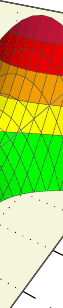
\begin{tikzpicture}%
%\begin{pgfpicture}{-4.1128cm}{-4.8433cm}{3.8872cm}{3.1567cm}%
\pgfsetxvec{\pgfxy(0.4,0)}
\pgfsetyvec{\pgfxy(0,0.4)}
\useasboundingbox (--4.1128,-4.8433)--(3.8872,3.1567);
%fond  (Utilisateur)
\pgfsetstrokecolor{rgb,1:red,0;green,0;blue,0}
\pgfsetlinewidth{0.4pt} 
\pgfsetroundjoin \pgfmoveto{\pgfxy(6.1423,-1.9292)}\pgflineto{\pgfxy(7.456,3.1538)}\pgflineto{\pgfxy(-0.5824,4.7051)}
\pgflineto{\pgfxy(-8.2181,2.5811)}\pgflineto{\pgfxy(-6.6504,-2.813)}\pgflineto{\pgfxy(1.0909,-8.8139)}
\pgfclosepath
\pgfsetfillcolor{rgb,1:red,0.9608;green,0.9608;blue,0.8627}
\pgffill
%boite  (Utilisateur)
\pgfsetstrokecolor{rgb,1:red,0.498;green,0.498;blue,0.498}
\pgfmoveto{\pgfxy(-0.5824,4.7051)}\pgflineto{\pgfxy(-8.2181,2.5811)}\pgflineto{\pgfxy(1.5359,-1.9284)}
\pgflineto{\pgfxy(7.456,3.1538)}\pgflineto{\pgfxy(-0.5824,4.7051)}
\pgfstroke
\pgfmoveto{\pgfxy(7.456,3.1538)}
\pgflineto{\pgfxy(1.5359,-1.9284)}\pgflineto{\pgfxy(1.0909,-8.8139)}\pgflineto{\pgfxy(6.1423,-1.9292)}
\pgflineto{\pgfxy(7.456,3.1538)}
\pgfstroke
\pgfmoveto{\pgfxy(-8.2181,2.5811)}\pgflineto{\pgfxy(-6.6504,-2.813)}
\pgflineto{\pgfxy(1.0909,-8.8139)}\pgflineto{\pgfxy(1.5359,-1.9284)}\pgflineto{\pgfxy(-8.2181,2.5811)}
\pgfstroke
%AxeOx  (Utilisateur)
\pgfsetstrokecolor{rgb,1:red,0;green,0;blue,0}
\pgfxyline(6.1423,-1.9292)(1.0909,-8.8139)
\pgfputat{\pgfxy(5.2371,-6.3003)}{\pgftext[top]{\color{rgb,1:red,0;green,0;blue,0}\scriptsize $x$}}\pgfstroke
\pgfputat{\pgfxy(6.7752,-2.3542)}{\pgftext[left,top]{\color{rgb,1:red,0;green,0;blue,0}\scriptsize $-2$}}\pgfstroke
\pgfputat{\pgfxy(6.1288,-3.2861)}{\pgftext[left,top]{\color{rgb,1:red,0;green,0;blue,0}\scriptsize $-1$}}\pgfstroke
\pgfputat{\pgfxy(5.3606,-4.3937)}{\pgftext[left,top]{\color{rgb,1:red,0;green,0;blue,0}\scriptsize $0$}}\pgfstroke
\pgfputat{\pgfxy(4.4324,-5.7319)}{\pgftext[left,top]{\color{rgb,1:red,0;green,0;blue,0}\scriptsize $1$}}\pgfstroke
\pgfputat{\pgfxy(3.2886,-7.3811)}{\pgftext[left,top]{\color{rgb,1:red,0;green,0;blue,0}\scriptsize $2$}}\pgfstroke
\pgfputat{\pgfxy(1.844,-9.4639)}{\pgftext[left,top]{\color{rgb,1:red,0;green,0;blue,0}\scriptsize $3$}}\pgfstroke
\pgfxyline(6.1423,-1.9292)(6.4805,-2.0596)\pgfxyline(5.4757,-2.8378)(5.8342,-2.9914)\pgfxyline(4.6851,-3.9153)(5.066,-4.0991)
\pgfxyline(3.7325,-5.2136)(4.1378,-5.4373)\pgfxyline(2.5625,-6.8082)(2.994,-7.0865)\pgfxyline(1.0909,-8.8139)(1.5494,-9.1693)
\pgfsetroundcap \pgfsetdash{{0pt}{3pt}}{0pt}
\pgfmoveto{\pgfxy(5.4757,-2.8378)}\pgflineto{\pgfxy(-1.4221,0.1186)}\pgflineto{\pgfxy(-1.6583,4.4058)}
\pgfstroke
\pgfmoveto{\pgfxy(4.6851,-3.9153)}\pgflineto{\pgfxy(-2.464,-0.4656)}\pgflineto{\pgfxy(-2.9058,4.0588)}
\pgfstroke
\pgfmoveto{\pgfxy(3.7325,-5.2136)}\pgflineto{\pgfxy(-3.657,-1.1345)}\pgflineto{\pgfxy(-4.3696,3.6516)}
\pgfstroke
\pgfmoveto{\pgfxy(2.5625,-6.8082)}\pgflineto{\pgfxy(-5.0366,-1.9081)}\pgflineto{\pgfxy(-6.1112,3.1672)}
\pgfstroke
%AxeOy  (Utilisateur)
\pgfsetbuttcap \pgfsetdash{}{0pt}
\pgfxyline(-6.6504,-2.813)(1.0909,-8.8139)
\pgfputat{\pgfxy(-4.3856,-7.0882)}{\pgftext[top]{\color{rgb,1:red,0;green,0;blue,0}\scriptsize $y$}}\pgfstroke
\pgfputat{\pgfxy(-7.3287,-3.3228)}{\pgftext[right,top]{\color{rgb,1:red,0;green,0;blue,0}\scriptsize $-2.5$}}\pgfstroke
\pgfputat{\pgfxy(-6.2413,-4.2041)}{\pgftext[right,top]{\color{rgb,1:red,0;green,0;blue,0}\scriptsize $-1.5$}}\pgfstroke
\pgfputat{\pgfxy(-4.9781,-5.2278)}{\pgftext[right,top]{\color{rgb,1:red,0;green,0;blue,0}\scriptsize $-0.5$}}\pgfstroke
\pgfputat{\pgfxy(-3.4928,-6.4315)}{\pgftext[right,top]{\color{rgb,1:red,0;green,0;blue,0}\scriptsize $0.5$}}\pgfstroke
\pgfputat{\pgfxy(-1.7211,-7.8673)}{\pgftext[right,top]{\color{rgb,1:red,0;green,0;blue,0}\scriptsize $1.5$}}\pgfstroke
\pgfputat{\pgfxy(0.4287,-9.6096)}{\pgftext[right,top]{\color{rgb,1:red,0;green,0;blue,0}\scriptsize $2.5$}}\pgfstroke
\pgfxyline(-6.6504,-2.813)(-7.034,-3.0282)\pgfxyline(-5.5562,-3.6612)(-5.9466,-3.9094)\pgfxyline(-4.2888,-4.6437)(-4.6835,-4.9331)
\pgfxyline(-2.8037,-5.7949)(-3.1982,-6.1369)\pgfxyline(-1.0394,-7.1625)(-1.4264,-7.5727)\pgfxyline(1.0909,-8.8139)(0.7233,-9.3149)
\pgfsetroundcap \pgfsetdash{{0pt}{3pt}}{0pt}
\pgfmoveto{\pgfxy(-5.5562,-3.6612)}\pgflineto{\pgfxy(0.5571,0.224)}\pgflineto{\pgfxy(0.6483,4.4676)}
\pgfstroke
\pgfmoveto{\pgfxy(-4.2888,-4.6437)}\pgflineto{\pgfxy(1.7312,-0.2286)}\pgflineto{\pgfxy(2.0323,4.2005)}
\pgfstroke
\pgfmoveto{\pgfxy(-2.8037,-5.7949)}\pgflineto{\pgfxy(3.0368,-0.7319)}\pgflineto{\pgfxy(3.6001,3.8979)}
\pgfstroke
\pgfmoveto{\pgfxy(-1.0394,-7.1625)}\pgflineto{\pgfxy(4.4974,-1.295)}\pgflineto{\pgfxy(5.3909,3.5523)}
\pgfstroke
%AxeOz  (Utilisateur)
\pgfsetbuttcap \pgfsetdash{}{0pt}
\pgfxyline(-6.6504,-2.813)(-8.2181,2.5811)\pgfxyline(6.1423,-1.9292)(7.456,3.1538)\pgfxyline(-0.5044,0.6332)(-0.5824,4.7051)
\pgfputat{\pgfxy(-9.0296,-0.1248)}{\pgftext[right]{\color{rgb,1:red,0;green,0;blue,0}\scriptsize $z$}}\pgfstroke
\pgfputat{\pgfxy(-7.1069,-2.6529)}{\pgftext[right]{\color{rgb,1:red,0;green,0;blue,0}\scriptsize $0$}}\pgfstroke
\pgfputat{\pgfxy(-7.5656,-1.1113)}{\pgftext[right]{\color{rgb,1:red,0;green,0;blue,0}\scriptsize $1$}}\pgfstroke
\pgfputat{\pgfxy(-8.0902,0.6514)}{\pgftext[right]{\color{rgb,1:red,0;green,0;blue,0}\scriptsize $2$}}\pgfstroke
\pgfputat{\pgfxy(-8.6958,2.6864)}{\pgftext[right]{\color{rgb,1:red,0;green,0;blue,0}\scriptsize $3$}}\pgfstroke
\pgfxyline(-6.6504,-2.813)(-6.8569,-2.6529)\pgfxyline(-7.102,-1.2592)(-7.3156,-1.1113)\pgfxyline(-7.6194,0.5211)(-7.8402,0.6514)
\pgfxyline(-8.2181,2.5811)(-8.4458,2.6864)
\pgfmoveto{\pgfxy(-6.6504,-2.813)}\pgflineto{\pgfxy(-0.5044,0.6332)}\pgflineto{\pgfxy(6.1423,-1.9292)}
\pgfstroke
\pgfmoveto{\pgfxy(-8.2181,2.5811)}\pgflineto{\pgfxy(-0.5824,4.7051)}\pgflineto{\pgfxy(7.456,3.1538)}
\pgfstroke
\pgfsetroundcap \pgfsetdash{{0pt}{3pt}}{0pt}
\pgfmoveto{\pgfxy(-7.102,-1.2592)}\pgflineto{\pgfxy(-0.5279,1.8637)}\pgflineto{\pgfxy(6.5256,-0.4463)}
\pgfstroke
\pgfmoveto{\pgfxy(-7.6194,0.5211)}\pgflineto{\pgfxy(-0.5538,3.2147)}\pgflineto{\pgfxy(6.9598,1.234)}
\pgfstroke
%Surf  (Utilisateur)
\pgfsetstrokecolor{rgb,1:red,0.2471;green,0.2471;blue,0.2471}
\pgfsetlinewidth{0.1pt} 
\pgfsetbuttcap \pgfsetdash{}{0pt}
\pgfmoveto{\pgfxy(1.4485,-0.2762)}\pgflineto{\pgfxy(1.4652,-0.2353)}\pgflineto{\pgfxy(1.6303,0.2394)}
\pgflineto{\pgfxy(1.4856,-0.1339)}\pgflineto{\pgfxy(1.4485,-0.2762)}
\pgfsetfillcolor{rgb,1:red,0;green,0.051;blue,0}
\pgffillstroke
\pgfmoveto{\pgfxy(1.4355,-0.3012)}\pgflineto{\pgfxy(1.4652,-0.2353)}\pgflineto{\pgfxy(1.4485,-0.2762)}
\pgflineto{\pgfxy(1.4355,-0.3012)}
\pgfsetfillcolor{rgb,1:red,0.098;green,0.2;blue,0.098}
\pgffillstroke
\pgfmoveto{\pgfxy(1.4652,-0.2353)}\pgflineto{\pgfxy(1.4355,-0.3012)}\pgflineto{\pgfxy(1.3905,-0.4152)}
\pgflineto{\pgfxy(1.557,-0.0745)}\pgflineto{\pgfxy(1.7222,0.326)}\pgflineto{\pgfxy(1.4652,-0.2353)}
\pgfsetfillcolor{rgb,1:red,0;green,0.1098;blue,0}
\pgffillstroke
\pgfmoveto{\pgfxy(1.6303,0.2394)}\pgflineto{\pgfxy(1.4652,-0.2353)}\pgflineto{\pgfxy(1.7222,0.326)}
\pgflineto{\pgfxy(1.8969,0.86)}\pgflineto{\pgfxy(1.6303,0.2394)}
\pgfsetfillcolor{rgb,1:red,0;green,0.0549;blue,0}
\pgffillstroke
\pgfmoveto{\pgfxy(1.3005,-0.5463)}\pgflineto{\pgfxy(1.3981,-0.3596)}\pgflineto{\pgfxy(1.557,-0.0745)}
\pgflineto{\pgfxy(1.3905,-0.4152)}\pgflineto{\pgfxy(1.3005,-0.5463)}
\pgfsetfillcolor{rgb,1:red,0.0902;green,0.1804;blue,0.0902}
\pgffillstroke
\pgfmoveto{\pgfxy(1.1736,-0.667)}\pgflineto{\pgfxy(1.2427,-0.5436)}\pgflineto{\pgfxy(1.3981,-0.3596)}
\pgflineto{\pgfxy(1.3005,-0.5463)}\pgflineto{\pgfxy(1.1736,-0.667)}
\pgfsetfillcolor{rgb,1:red,0.1451;green,0.2902;blue,0.1451}
\pgffillstroke
\pgfmoveto{\pgfxy(1.8969,0.86)}\pgflineto{\pgfxy(1.7222,0.326)}\pgflineto{\pgfxy(1.9916,0.8438)}
\pgflineto{\pgfxy(2.0103,0.9043)}\pgflineto{\pgfxy(1.9841,1.041)}\pgflineto{\pgfxy(1.8969,0.86)}
\pgfsetfillcolor{rgb,1:red,0;green,0.1843;blue,0}
\pgffillstroke
\pgfmoveto{\pgfxy(1.7222,0.326)}\pgflineto{\pgfxy(1.557,-0.0745)}\pgflineto{\pgfxy(1.8181,0.389)}
\pgflineto{\pgfxy(1.9916,0.8438)}\pgflineto{\pgfxy(1.7222,0.326)}
\pgfsetfillcolor{rgb,1:red,0;green,0.0745;blue,0}
\pgffillstroke
\pgfmoveto{\pgfxy(1.557,-0.0745)}\pgflineto{\pgfxy(1.3981,-0.3596)}\pgflineto{\pgfxy(1.6529,0.0564)}
\pgflineto{\pgfxy(1.8181,0.389)}\pgflineto{\pgfxy(1.557,-0.0745)}
\pgfsetfillcolor{rgb,1:red,0;green,0.102;blue,0}
\pgffillstroke
\pgfmoveto{\pgfxy(1.0062,-0.7752)}\pgflineto{\pgfxy(1.0885,-0.6385)}\pgflineto{\pgfxy(1.2427,-0.5436)}
\pgflineto{\pgfxy(1.1736,-0.667)}\pgflineto{\pgfxy(1.0062,-0.7752)}
\pgfsetfillcolor{rgb,1:red,0.1922;green,0.3843;blue,0.1922}
\pgffillstroke
\pgfmoveto{\pgfxy(1.3981,-0.3596)}\pgflineto{\pgfxy(1.2427,-0.5436)}\pgflineto{\pgfxy(1.4928,-0.1702)}
\pgflineto{\pgfxy(1.6529,0.0564)}\pgflineto{\pgfxy(1.3981,-0.3596)}
\pgfsetfillcolor{rgb,1:red,0.1137;green,0.2275;blue,0.1137}
\pgffillstroke
\pgfmoveto{\pgfxy(2.0103,0.9043)}\pgflineto{\pgfxy(1.9916,0.8438)}\pgflineto{\pgfxy(2.0176,0.8871)}
\pgflineto{\pgfxy(2.0103,0.9043)}
\pgfsetfillcolor{rgb,1:red,0;green,0.302;blue,0}
\pgffillstroke
\pgfmoveto{\pgfxy(0.7938,-0.8682)}\pgflineto{\pgfxy(0.9333,-0.6541)}\pgflineto{\pgfxy(1.0885,-0.6385)}
\pgflineto{\pgfxy(1.0062,-0.7752)}\pgflineto{\pgfxy(0.7938,-0.8682)}
\pgfsetfillcolor{rgb,1:red,0.2314;green,0.4627;blue,0.2314}
\pgffillstroke
\pgfmoveto{\pgfxy(1.9916,0.8438)}\pgflineto{\pgfxy(1.8181,0.389)}\pgflineto{\pgfxy(2.0449,0.7295)}
\pgflineto{\pgfxy(2.0176,0.8871)}\pgflineto{\pgfxy(1.9916,0.8438)}
\pgfsetfillcolor{rgb,1:red,0;green,0.2235;blue,0}
\pgffillstroke
\pgfmoveto{\pgfxy(1.2427,-0.5436)}\pgflineto{\pgfxy(1.0885,-0.6385)}\pgflineto{\pgfxy(1.3353,-0.3039)}
\pgflineto{\pgfxy(1.4928,-0.1702)}\pgflineto{\pgfxy(1.2427,-0.5436)}
\pgfsetfillcolor{rgb,1:red,0.1686;green,0.3373;blue,0.1686}
\pgffillstroke
\pgfmoveto{\pgfxy(0.5328,-0.9435)}\pgflineto{\pgfxy(0.5412,-0.9288)}\pgflineto{\pgfxy(0.5554,-0.9365)}
\pgflineto{\pgfxy(0.5328,-0.9435)}
\pgfsetfillcolor{rgb,1:red,0.2863;green,0.5725;blue,0.2863}
\pgffillstroke
\pgfmoveto{\pgfxy(0.5554,-0.9365)}\pgflineto{\pgfxy(0.5412,-0.9288)}\pgflineto{\pgfxy(0.7752,-0.5992)}
\pgflineto{\pgfxy(0.9333,-0.6541)}\pgflineto{\pgfxy(0.7938,-0.8682)}\pgflineto{\pgfxy(0.5554,-0.9365)}
\pgfsetfillcolor{rgb,1:red,0.2784;green,0.5569;blue,0.2784}
\pgffillstroke
\pgfmoveto{\pgfxy(1.8181,0.389)}\pgflineto{\pgfxy(1.6529,0.0564)}\pgflineto{\pgfxy(1.9171,0.4126)}
\pgflineto{\pgfxy(2.0407,0.688)}\pgflineto{\pgfxy(2.0449,0.7295)}\pgflineto{\pgfxy(1.8181,0.389)}
\pgfsetfillcolor{rgb,1:red,0;green,0.1176;blue,0}
\pgffillstroke
\pgfmoveto{\pgfxy(0.2395,-1.0075)}\pgflineto{\pgfxy(0.3782,-0.782)}\pgflineto{\pgfxy(0.5412,-0.9288)}
\pgflineto{\pgfxy(0.5328,-0.9435)}\pgflineto{\pgfxy(0.2395,-1.0075)}
\pgfsetfillcolor{rgb,1:red,0.302;green,0.6078;blue,0.302}
\pgffillstroke
\pgfmoveto{\pgfxy(1.0885,-0.6385)}\pgflineto{\pgfxy(0.9333,-0.6541)}\pgflineto{\pgfxy(1.1781,-0.3559)}
\pgflineto{\pgfxy(1.3353,-0.3039)}\pgflineto{\pgfxy(1.0885,-0.6385)}
\pgfsetfillcolor{rgb,1:red,0.2118;green,0.4235;blue,0.2118}
\pgffillstroke
\pgfmoveto{\pgfxy(1.6529,0.0564)}\pgflineto{\pgfxy(1.4928,-0.1702)}\pgflineto{\pgfxy(1.7518,0.1402)}
\pgflineto{\pgfxy(1.9171,0.4126)}\pgflineto{\pgfxy(1.6529,0.0564)}
\pgfsetfillcolor{rgb,1:red,0;green,0.0588;blue,0}
\pgffillstroke
\pgfmoveto{\pgfxy(-0.0898,-1.0576)}\pgflineto{\pgfxy(-0.0158,-0.9185)}\pgflineto{\pgfxy(0.0698,-1.0313)}
\pgflineto{\pgfxy(-0.0898,-1.0576)}
\pgfsetfillcolor{rgb,1:red,0.3294;green,0.6588;blue,0.3294}
\pgffillstroke
\pgfmoveto{\pgfxy(-0.4436,-1.0984)}\pgflineto{\pgfxy(-0.4086,-1.0222)}\pgflineto{\pgfxy(-0.3675,-1.0883)}
\pgflineto{\pgfxy(-0.4436,-1.0984)}
\pgfsetfillcolor{rgb,1:red,0.3451;green,0.6941;blue,0.3451}
\pgffillstroke
\pgfmoveto{\pgfxy(-0.8124,-1.1338)}\pgflineto{\pgfxy(-0.8014,-1.1061)}\pgflineto{\pgfxy(-0.7875,-1.1309)}
\pgflineto{\pgfxy(-0.8124,-1.1338)}
\pgfsetfillcolor{rgb,1:red,0.3569;green,0.7176;blue,0.3569}
\pgffillstroke
\pgfmoveto{\pgfxy(0.0698,-1.0313)}\pgflineto{\pgfxy(-0.0158,-0.9185)}\pgflineto{\pgfxy(0.2077,-0.5814)}
\pgflineto{\pgfxy(0.3782,-0.782)}\pgflineto{\pgfxy(0.2395,-1.0075)}\pgflineto{\pgfxy(0.0698,-1.0313)}
\pgfsetfillcolor{rgb,1:red,0.3255;green,0.6471;blue,0.3255}
\pgffillstroke
\pgfmoveto{\pgfxy(1.4928,-0.1702)}\pgflineto{\pgfxy(1.3353,-0.3039)}\pgflineto{\pgfxy(1.5906,-0.0358)}
\pgflineto{\pgfxy(1.7518,0.1402)}\pgflineto{\pgfxy(1.4928,-0.1702)}
\pgfsetfillcolor{rgb,1:red,0.098;green,0.1961;blue,0.098}
\pgffillstroke
\pgfmoveto{\pgfxy(2.0407,0.688)}\pgflineto{\pgfxy(1.9171,0.4126)}\pgflineto{\pgfxy(2.0643,0.5686)}
\pgflineto{\pgfxy(2.0407,0.688)}
\pgfsetfillcolor{rgb,1:red,0;green,0.298;blue,0}
\pgffillstroke
\pgfmoveto{\pgfxy(-3.0471,-1.3707)}\pgflineto{\pgfxy(-3.0287,-1.249)}\pgflineto{\pgfxy(-2.9554,-1.3569)}
\pgflineto{\pgfxy(-3.0471,-1.3707)}
\pgfsetfillcolor{rgb,1:red,0.3686;green,0.7373;blue,0.3686}
\pgffillstroke
\pgfmoveto{\pgfxy(-0.3675,-1.0883)}\pgflineto{\pgfxy(-0.4086,-1.0222)}\pgflineto{\pgfxy(-0.1966,-0.6467)}
\pgflineto{\pgfxy(-0.0158,-0.9185)}\pgflineto{\pgfxy(-0.0898,-1.0576)}\pgflineto{\pgfxy(-0.3675,-1.0883)}
\pgfsetfillcolor{rgb,1:red,0.3412;green,0.6863;blue,0.3412}
\pgffillstroke
\pgfmoveto{\pgfxy(-0.7875,-1.1309)}\pgflineto{\pgfxy(-0.8014,-1.1061)}\pgflineto{\pgfxy(-0.6021,-0.6913)}
\pgflineto{\pgfxy(-0.4086,-1.0222)}\pgflineto{\pgfxy(-0.4436,-1.0984)}\pgflineto{\pgfxy(-0.7875,-1.1309)}
\pgfsetfillcolor{rgb,1:red,0.3529;green,0.7098;blue,0.3529}
\pgffillstroke
\pgfmoveto{\pgfxy(0.5412,-0.9288)}\pgflineto{\pgfxy(0.3782,-0.782)}\pgflineto{\pgfxy(0.6122,-0.4824)}
\pgflineto{\pgfxy(0.7752,-0.5992)}\pgflineto{\pgfxy(0.5412,-0.9288)}
\pgfsetfillcolor{rgb,1:red,0.2941;green,0.5882;blue,0.2941}
\pgffillstroke
\pgfmoveto{\pgfxy(-2.6857,-1.3206)}\pgflineto{\pgfxy(-2.6353,-1.0584)}\pgflineto{\pgfxy(-2.4886,-1.2954)}
\pgflineto{\pgfxy(-2.6857,-1.3206)}
\pgfsetfillcolor{rgb,1:red,0.3686;green,0.7412;blue,0.3686}
\pgffillstroke
\pgfmoveto{\pgfxy(-1.1884,-1.1672)}\pgflineto{\pgfxy(-1.0093,-0.7283)}\pgflineto{\pgfxy(-0.8014,-1.1061)}
\pgflineto{\pgfxy(-0.8124,-1.1338)}\pgflineto{\pgfxy(-1.1884,-1.1672)}
\pgfsetfillcolor{rgb,1:red,0.3569;green,0.7137;blue,0.3569}
\pgffillstroke
\pgfmoveto{\pgfxy(-2.3173,-1.2764)}\pgflineto{\pgfxy(-2.2333,-0.9231)}\pgflineto{\pgfxy(-2.0465,-1.2466)}
\pgflineto{\pgfxy(-2.3173,-1.2764)}
\pgfsetfillcolor{rgb,1:red,0.3686;green,0.7373;blue,0.3686}
\pgffillstroke
\pgfmoveto{\pgfxy(-3.736,-1.4981)}\pgflineto{\pgfxy(-3.7029,-1.1905)}\pgflineto{\pgfxy(-3.4679,-1.4425)}
\pgflineto{\pgfxy(-3.736,-1.4981)}
\pgfsetfillcolor{rgb,1:red,0.3529;green,0.7059;blue,0.3529}
\pgffillstroke
\pgfmoveto{\pgfxy(-1.9435,-1.2371)}\pgflineto{\pgfxy(-1.8266,-0.8313)}\pgflineto{\pgfxy(-1.62,-1.2055)}
\pgflineto{\pgfxy(-1.9435,-1.2371)}
\pgfsetfillcolor{rgb,1:red,0.3686;green,0.7333;blue,0.3686}
\pgffillstroke
\pgfmoveto{\pgfxy(-1.5662,-1.2012)}\pgflineto{\pgfxy(-1.4179,-0.7707)}\pgflineto{\pgfxy(-1.2024,-1.1682)}
\pgflineto{\pgfxy(-1.5662,-1.2012)}
\pgfsetfillcolor{rgb,1:red,0.3647;green,0.7294;blue,0.3647}
\pgffillstroke
\pgfmoveto{\pgfxy(0.9333,-0.6541)}\pgflineto{\pgfxy(0.7752,-0.5992)}\pgflineto{\pgfxy(1.0189,-0.3361)}
\pgflineto{\pgfxy(1.1781,-0.3559)}\pgflineto{\pgfxy(0.9333,-0.6541)}
\pgfsetfillcolor{rgb,1:red,0.2431;green,0.4863;blue,0.2431}
\pgffillstroke
\pgfmoveto{\pgfxy(-4.3723,-1.6714)}\pgflineto{\pgfxy(-4.3562,-1.4345)}\pgflineto{\pgfxy(-4.0787,-1.5808)}
\pgflineto{\pgfxy(-4.3723,-1.6714)}
\pgfsetfillcolor{rgb,1:red,0.3176;green,0.6392;blue,0.3176}
\pgffillstroke
\pgfmoveto{\pgfxy(-3.3982,-1.4291)}\pgflineto{\pgfxy(-3.3177,-0.8816)}\pgflineto{\pgfxy(-3.0287,-1.249)}
\pgflineto{\pgfxy(-3.0471,-1.3707)}\pgflineto{\pgfxy(-3.3982,-1.4291)}
\pgfsetfillcolor{rgb,1:red,0.3569;green,0.7176;blue,0.3569}
\pgffillstroke
\pgfmoveto{\pgfxy(1.9171,0.4126)}\pgflineto{\pgfxy(1.7518,0.1402)}\pgflineto{\pgfxy(2.0178,0.3794)}
\pgflineto{\pgfxy(2.053,0.4456)}\pgflineto{\pgfxy(2.0643,0.5686)}\pgflineto{\pgfxy(1.9171,0.4126)}
\pgfsetfillcolor{rgb,1:red,0;green,0.2039;blue,0}
\pgffillstroke
\pgfmoveto{\pgfxy(5.8509,-1.4726)}\pgflineto{\pgfxy(5.6792,-2.0283)}\pgflineto{\pgfxy(5.9309,-2.0347)}
\pgflineto{\pgfxy(5.8509,-1.4726)}
\pgfsetfillcolor{rgb,1:red,0;green,0.9569;blue,0}
\pgffillstroke
\pgfmoveto{\pgfxy(1.3353,-0.3039)}\pgflineto{\pgfxy(1.1781,-0.3559)}\pgflineto{\pgfxy(1.431,-0.128)}
\pgflineto{\pgfxy(1.5906,-0.0358)}\pgflineto{\pgfxy(1.3353,-0.3039)}
\pgfsetfillcolor{rgb,1:red,0.1529;green,0.3059;blue,0.1529}
\pgffillstroke
\pgfmoveto{\pgfxy(-2.9554,-1.3569)}\pgflineto{\pgfxy(-3.0287,-1.249)}\pgflineto{\pgfxy(-2.9156,-0.6536)}
\pgflineto{\pgfxy(-2.6353,-1.0584)}\pgflineto{\pgfxy(-2.6857,-1.3206)}\pgflineto{\pgfxy(-2.9554,-1.3569)}
\pgfsetfillcolor{rgb,1:red,0.3686;green,0.7333;blue,0.3686}
\pgffillstroke
\pgfmoveto{\pgfxy(-4.0642,-1.5765)}\pgflineto{\pgfxy(-3.9994,-0.9553)}\pgflineto{\pgfxy(-3.7029,-1.1905)}
\pgflineto{\pgfxy(-3.736,-1.4981)}\pgflineto{\pgfxy(-4.0642,-1.5765)}
\pgfsetfillcolor{rgb,1:red,0.3333;green,0.6667;blue,0.3333}
\pgffillstroke
\pgfmoveto{\pgfxy(5.3635,-1.8058)}\pgflineto{\pgfxy(5.2973,-2.0179)}\pgflineto{\pgfxy(5.4003,-2.0166)}
\pgflineto{\pgfxy(5.3635,-1.8058)}
\pgfsetfillcolor{rgb,1:red,0;green,0.9647;blue,0}
\pgffillstroke
\pgfmoveto{\pgfxy(-2.4886,-1.2954)}\pgflineto{\pgfxy(-2.6353,-1.0584)}\pgflineto{\pgfxy(-2.5016,-0.4967)}
\pgflineto{\pgfxy(-2.2333,-0.9231)}\pgflineto{\pgfxy(-2.3173,-1.2764)}\pgflineto{\pgfxy(-2.4886,-1.2954)}
\pgfsetfillcolor{rgb,1:red,0.3686;green,0.7373;blue,0.3686}
\pgffillstroke
\pgfmoveto{\pgfxy(-4.6634,-1.7821)}\pgflineto{\pgfxy(-4.6383,-1.3991)}\pgflineto{\pgfxy(-4.3562,-1.4345)}
\pgflineto{\pgfxy(-4.3723,-1.6714)}\pgflineto{\pgfxy(-4.6634,-1.7821)}
\pgfsetfillcolor{rgb,1:red,0.2824;green,0.5647;blue,0.2824}
\pgffillstroke
\pgfmoveto{\pgfxy(-2.0465,-1.2466)}\pgflineto{\pgfxy(-2.2333,-0.9231)}\pgflineto{\pgfxy(-2.0805,-0.3991)}
\pgflineto{\pgfxy(-1.8266,-0.8313)}\pgflineto{\pgfxy(-1.9435,-1.2371)}\pgflineto{\pgfxy(-2.0465,-1.2466)}
\pgfsetfillcolor{rgb,1:red,0.3686;green,0.7333;blue,0.3686}
\pgffillstroke
\pgfmoveto{\pgfxy(1.7518,0.1402)}\pgflineto{\pgfxy(1.5906,-0.0358)}\pgflineto{\pgfxy(1.8525,0.158)}
\pgflineto{\pgfxy(2.0178,0.3794)}\pgflineto{\pgfxy(1.7518,0.1402)}
\pgfsetfillcolor{rgb,1:red,0;green,0.0824;blue,0}
\pgffillstroke
\pgfmoveto{\pgfxy(-1.62,-1.2055)}\pgflineto{\pgfxy(-1.8266,-0.8313)}\pgflineto{\pgfxy(-1.6561,-0.348)}
\pgflineto{\pgfxy(-1.4179,-0.7707)}\pgflineto{\pgfxy(-1.5662,-1.2012)}\pgflineto{\pgfxy(-1.62,-1.2055)}
\pgfsetfillcolor{rgb,1:red,0.3647;green,0.7294;blue,0.3647}
\pgffillstroke
\pgfmoveto{\pgfxy(-1.2024,-1.1682)}\pgflineto{\pgfxy(-1.4179,-0.7707)}\pgflineto{\pgfxy(-1.2314,-0.3298)}
\pgflineto{\pgfxy(-1.0093,-0.7283)}\pgflineto{\pgfxy(-1.1884,-1.1672)}\pgflineto{\pgfxy(-1.2024,-1.1682)}
\pgfsetfillcolor{rgb,1:red,0.3608;green,0.7216;blue,0.3608}
\pgffillstroke
\pgfmoveto{\pgfxy(5.7042,-0.6794)}\pgflineto{\pgfxy(5.3635,-1.8058)}\pgflineto{\pgfxy(5.4003,-2.0166)}
\pgflineto{\pgfxy(5.6792,-2.0283)}\pgflineto{\pgfxy(5.8509,-1.4726)}\pgflineto{\pgfxy(5.7042,-0.6794)}
\pgfsetfillcolor{rgb,1:red,0;green,0.9569;blue,0}
\pgffillstroke
\pgfmoveto{\pgfxy(-3.4679,-1.4425)}\pgflineto{\pgfxy(-3.7029,-1.1905)}\pgflineto{\pgfxy(-3.6142,-0.5775)}
\pgflineto{\pgfxy(-3.3177,-0.8816)}\pgflineto{\pgfxy(-3.3982,-1.4291)}\pgflineto{\pgfxy(-3.4679,-1.4425)}
\pgfsetfillcolor{rgb,1:red,0.3529;green,0.702;blue,0.3529}
\pgffillstroke
\pgfmoveto{\pgfxy(4.9114,-2.0089)}\pgflineto{\pgfxy(4.9093,-2.0155)}\pgflineto{\pgfxy(4.9127,-2.0153)}
\pgflineto{\pgfxy(4.9114,-2.0089)}
\pgfsetfillcolor{rgb,1:red,0;green,0.9686;blue,0}
\pgffillstroke
\pgfmoveto{\pgfxy(2.053,0.4456)}\pgflineto{\pgfxy(2.0178,0.3794)}\pgflineto{\pgfxy(2.0656,0.4077)}
\pgflineto{\pgfxy(2.053,0.4456)}
\pgfsetfillcolor{rgb,1:red,0;green,0.4196;blue,0}
\pgffillstroke
\pgfmoveto{\pgfxy(6.1855,-0.3635)}\pgflineto{\pgfxy(5.8509,-1.4726)}\pgflineto{\pgfxy(5.9309,-2.0347)}
\pgflineto{\pgfxy(6.0582,-2.0438)}\pgflineto{\pgfxy(6.3861,-0.9859)}\pgflineto{\pgfxy(6.2943,-0.3706)}
\pgflineto{\pgfxy(6.1855,-0.3635)}
\pgfsetfillcolor{rgb,1:red,0;green,0.949;blue,0}
\pgffillstroke
\pgfmoveto{\pgfxy(5.201,-1.0704)}\pgflineto{\pgfxy(4.9114,-2.0089)}\pgflineto{\pgfxy(4.9127,-2.0153)}
\pgflineto{\pgfxy(5.2973,-2.0179)}\pgflineto{\pgfxy(5.3635,-1.8058)}\pgflineto{\pgfxy(5.201,-1.0704)}
\pgfsetfillcolor{rgb,1:red,0;green,0.9647;blue,0}
\pgffillstroke
\pgfmoveto{\pgfxy(-4.0787,-1.5808)}\pgflineto{\pgfxy(-4.3562,-1.4345)}\pgflineto{\pgfxy(-4.2933,-0.8235)}
\pgflineto{\pgfxy(-3.9994,-0.9553)}\pgflineto{\pgfxy(-4.0642,-1.5765)}\pgflineto{\pgfxy(-4.0787,-1.5808)}
\pgfsetfillcolor{rgb,1:red,0.3176;green,0.6353;blue,0.3176}
\pgffillstroke
\pgfmoveto{\pgfxy(-4.9312,-1.9143)}\pgflineto{\pgfxy(-4.9038,-1.5029)}\pgflineto{\pgfxy(-4.6383,-1.3991)}
\pgflineto{\pgfxy(-4.6634,-1.7821)}\pgflineto{\pgfxy(-4.9312,-1.9143)}
\pgfsetfillcolor{rgb,1:red,0.2275;green,0.4549;blue,0.2275}
\pgffillstroke
\pgfmoveto{\pgfxy(0.3782,-0.782)}\pgflineto{\pgfxy(0.2077,-0.5814)}\pgflineto{\pgfxy(0.4426,-0.3119)}
\pgflineto{\pgfxy(0.6122,-0.4824)}\pgflineto{\pgfxy(0.3782,-0.782)}
\pgfsetfillcolor{rgb,1:red,0.302;green,0.6078;blue,0.302}
\pgffillstroke
\pgfmoveto{\pgfxy(-0.0158,-0.9185)}\pgflineto{\pgfxy(-0.1966,-0.6467)}\pgflineto{\pgfxy(0.0282,-0.3352)}
\pgflineto{\pgfxy(0.2077,-0.5814)}\pgflineto{\pgfxy(-0.0158,-0.9185)}
\pgfsetfillcolor{rgb,1:red,0.3255;green,0.6549;blue,0.3255}
\pgffillstroke
\pgfmoveto{\pgfxy(0.7752,-0.5992)}\pgflineto{\pgfxy(0.6122,-0.4824)}\pgflineto{\pgfxy(0.8559,-0.2537)}
\pgflineto{\pgfxy(1.0189,-0.3361)}\pgflineto{\pgfxy(0.7752,-0.5992)}
\pgfsetfillcolor{rgb,1:red,0.2627;green,0.5255;blue,0.2627}
\pgffillstroke
\pgfmoveto{\pgfxy(-0.4086,-1.0222)}\pgflineto{\pgfxy(-0.6021,-0.6913)}\pgflineto{\pgfxy(-0.3886,-0.337)}
\pgflineto{\pgfxy(-0.1966,-0.6467)}\pgflineto{\pgfxy(-0.4086,-1.0222)}
\pgfsetfillcolor{rgb,1:red,0.3412;green,0.6863;blue,0.3412}
\pgffillstroke
\pgfmoveto{\pgfxy(-0.8014,-1.1061)}\pgflineto{\pgfxy(-1.0093,-0.7283)}\pgflineto{\pgfxy(-0.8085,-0.3307)}
\pgflineto{\pgfxy(-0.6021,-0.6913)}\pgflineto{\pgfxy(-0.8014,-1.1061)}
\pgfsetfillcolor{rgb,1:red,0.3529;green,0.7059;blue,0.3529}
\pgffillstroke
\pgfmoveto{\pgfxy(1.1781,-0.3559)}\pgflineto{\pgfxy(1.0189,-0.3361)}\pgflineto{\pgfxy(1.2707,-0.1471)}
\pgflineto{\pgfxy(1.431,-0.128)}\pgflineto{\pgfxy(1.1781,-0.3559)}
\pgfsetfillcolor{rgb,1:red,0.1922;green,0.3843;blue,0.1922}
\pgffillstroke
\pgfmoveto{\pgfxy(4.7346,-1.3235)}\pgflineto{\pgfxy(4.5071,-2.0295)}\pgflineto{\pgfxy(4.9093,-2.0155)}
\pgflineto{\pgfxy(4.9114,-2.0089)}\pgflineto{\pgfxy(4.7346,-1.3235)}
\pgfsetfillcolor{rgb,1:red,0;green,0.9765;blue,0}
\pgffillstroke
\pgfmoveto{\pgfxy(1.5906,-0.0358)}\pgflineto{\pgfxy(1.431,-0.128)}\pgflineto{\pgfxy(1.6902,0.0224)}
\pgflineto{\pgfxy(1.8525,0.158)}\pgflineto{\pgfxy(1.5906,-0.0358)}
\pgfsetfillcolor{rgb,1:red,0.051;green,0.098;blue,0.051}
\pgffillstroke
\pgfmoveto{\pgfxy(-5.1668,-2.0754)}\pgflineto{\pgfxy(-5.1445,-1.7643)}\pgflineto{\pgfxy(-4.9038,-1.5029)}
\pgflineto{\pgfxy(-4.9312,-1.9143)}\pgflineto{\pgfxy(-5.1668,-2.0754)}
\pgfsetfillcolor{rgb,1:red,0.149;green,0.298;blue,0.149}
\pgffillstroke
\pgfmoveto{\pgfxy(2.0178,0.3794)}\pgflineto{\pgfxy(1.8525,0.158)}\pgflineto{\pgfxy(2.0565,0.2442)}
\pgflineto{\pgfxy(2.0656,0.4077)}\pgflineto{\pgfxy(2.0178,0.3794)}
\pgfsetfillcolor{rgb,1:red,0;green,0.3529;blue,0}
\pgffillstroke
\pgfmoveto{\pgfxy(-5.3587,-2.2762)}\pgflineto{\pgfxy(-5.352,-2.1956)}\pgflineto{\pgfxy(-5.1445,-1.7643)}
\pgflineto{\pgfxy(-5.1668,-2.0754)}\pgflineto{\pgfxy(-5.3587,-2.2762)}
\pgfsetfillcolor{rgb,1:red,0.0353;green,0.0667;blue,0.0353}
\pgffillstroke
\pgfmoveto{\pgfxy(-5.3892,-2.3309)}\pgflineto{\pgfxy(-5.352,-2.1956)}\pgflineto{\pgfxy(-5.3587,-2.2762)}
\pgflineto{\pgfxy(-5.3892,-2.3309)}
\pgfsetfillcolor{rgb,1:red,0.0902;green,0.1765;blue,0.0902}
\pgffillstroke
\pgfmoveto{\pgfxy(-3.0287,-1.249)}\pgflineto{\pgfxy(-3.3177,-0.8816)}\pgflineto{\pgfxy(-3.2067,-0.2958)}
\pgflineto{\pgfxy(-2.9156,-0.6536)}\pgflineto{\pgfxy(-3.0287,-1.249)}
\pgfsetfillcolor{rgb,1:red,0.3569;green,0.7137;blue,0.3569}
\pgffillstroke
\pgfmoveto{\pgfxy(4.2945,-1.4587)}\pgflineto{\pgfxy(4.0839,-2.0654)}\pgflineto{\pgfxy(4.4637,-2.0299)}
\pgflineto{\pgfxy(4.2945,-1.4587)}
\pgfsetfillcolor{rgb,1:red,0;green,0.9765;blue,0}
\pgffillstroke
\pgfmoveto{\pgfxy(5.8063,-0.3323)}\pgflineto{\pgfxy(5.7042,-0.6794)}\pgflineto{\pgfxy(5.8509,-1.4726)}
\pgflineto{\pgfxy(6.1855,-0.3635)}\pgflineto{\pgfxy(5.8063,-0.3323)}
\pgfsetfillcolor{rgb,1:red,0;green,0.949;blue,0}
\pgffillstroke
\pgfmoveto{\pgfxy(5.0153,-0.4053)}\pgflineto{\pgfxy(4.7346,-1.3235)}\pgflineto{\pgfxy(4.9114,-2.0089)}
\pgflineto{\pgfxy(5.201,-1.0704)}\pgflineto{\pgfxy(5.0153,-0.4053)}
\pgfsetfillcolor{rgb,1:red,0;green,0.9686;blue,0}
\pgffillstroke
\pgfmoveto{\pgfxy(4.5367,-0.7106)}\pgflineto{\pgfxy(4.2945,-1.4587)}\pgflineto{\pgfxy(4.4637,-2.0299)}
\pgflineto{\pgfxy(4.5071,-2.0295)}\pgflineto{\pgfxy(4.7346,-1.3235)}\pgflineto{\pgfxy(4.5367,-0.7106)}
\pgfsetfillcolor{rgb,1:red,0;green,0.9804;blue,0}
\pgffillstroke
\pgfmoveto{\pgfxy(5.429,-0.3021)}\pgflineto{\pgfxy(5.201,-1.0704)}\pgflineto{\pgfxy(5.3635,-1.8058)}
\pgflineto{\pgfxy(5.7042,-0.6794)}\pgflineto{\pgfxy(5.6174,-0.3136)}\pgflineto{\pgfxy(5.429,-0.3021)}
\pgfsetfillcolor{rgb,1:red,0;green,0.9608;blue,0}
\pgffillstroke
\pgfmoveto{\pgfxy(1.431,-0.128)}\pgflineto{\pgfxy(1.2707,-0.1471)}\pgflineto{\pgfxy(1.5285,-0.0392)}
\pgflineto{\pgfxy(1.6902,0.0224)}\pgflineto{\pgfxy(1.431,-0.128)}
\pgfsetfillcolor{rgb,1:red,0.102;green,0.2078;blue,0.102}
\pgffillstroke
\pgfmoveto{\pgfxy(1.0189,-0.3361)}\pgflineto{\pgfxy(0.8559,-0.2537)}\pgflineto{\pgfxy(1.1076,-0.1034)}
\pgflineto{\pgfxy(1.2707,-0.1471)}\pgflineto{\pgfxy(1.0189,-0.3361)}
\pgfsetfillcolor{rgb,1:red,0.2157;green,0.4275;blue,0.2157}
\pgffillstroke
\pgfmoveto{\pgfxy(-4.3562,-1.4345)}\pgflineto{\pgfxy(-4.6383,-1.3991)}\pgflineto{\pgfxy(-4.5774,-0.8191)}
\pgflineto{\pgfxy(-4.2933,-0.8235)}\pgflineto{\pgfxy(-4.3562,-1.4345)}
\pgfsetfillcolor{rgb,1:red,0.2784;green,0.5569;blue,0.2784}
\pgffillstroke
\pgfmoveto{\pgfxy(0.6122,-0.4824)}\pgflineto{\pgfxy(0.4426,-0.3119)}\pgflineto{\pgfxy(0.6872,-0.118)}
\pgflineto{\pgfxy(0.8559,-0.2537)}\pgflineto{\pgfxy(0.6122,-0.4824)}
\pgfsetfillcolor{rgb,1:red,0.2706;green,0.5451;blue,0.2706}
\pgffillstroke
\pgfmoveto{\pgfxy(5.6174,-0.3136)}\pgflineto{\pgfxy(5.7042,-0.6794)}\pgflineto{\pgfxy(5.8063,-0.3323)}
\pgflineto{\pgfxy(5.6174,-0.3136)}
\pgfsetfillcolor{rgb,1:red,0;green,0.9412;blue,0}
\pgffillstroke
\pgfmoveto{\pgfxy(1.8525,0.158)}\pgflineto{\pgfxy(1.6902,0.0224)}\pgflineto{\pgfxy(1.9533,0.0889)}
\pgflineto{\pgfxy(2.0011,0.1414)}\pgflineto{\pgfxy(2.0565,0.2442)}\pgflineto{\pgfxy(1.8525,0.158)}
\pgfsetfillcolor{rgb,1:red,0;green,0.2667;blue,0}
\pgffillstroke
\pgfmoveto{\pgfxy(4.0856,-0.8927)}\pgflineto{\pgfxy(3.8722,-1.4921)}\pgflineto{\pgfxy(4.0656,-2.0666)}
\pgflineto{\pgfxy(4.0839,-2.0654)}\pgflineto{\pgfxy(4.2945,-1.4587)}\pgflineto{\pgfxy(4.0856,-0.8927)}
\pgfsetfillcolor{rgb,1:red,0;green,0.9804;blue,0}
\pgffillstroke
\pgfmoveto{\pgfxy(0.2077,-0.5814)}\pgflineto{\pgfxy(0.0282,-0.3352)}\pgflineto{\pgfxy(0.2647,-0.0965)}
\pgflineto{\pgfxy(0.4426,-0.3119)}\pgflineto{\pgfxy(0.2077,-0.5814)}
\pgfsetfillcolor{rgb,1:red,0.3059;green,0.6118;blue,0.3059}
\pgffillstroke
\pgfmoveto{\pgfxy(3.8722,-1.4921)}\pgflineto{\pgfxy(3.6742,-1.9993)}\pgflineto{\pgfxy(3.7129,-2.1242)}
\pgflineto{\pgfxy(4.0656,-2.0666)}\pgflineto{\pgfxy(3.8722,-1.4921)}
\pgfsetfillcolor{rgb,1:red,0;green,0.9608;blue,0}
\pgffillstroke
\pgfmoveto{\pgfxy(-3.7029,-1.1905)}\pgflineto{\pgfxy(-3.9994,-0.9553)}\pgflineto{\pgfxy(-3.9133,-0.3605)}
\pgflineto{\pgfxy(-3.6142,-0.5775)}\pgflineto{\pgfxy(-3.7029,-1.1905)}
\pgfsetfillcolor{rgb,1:red,0.3333;green,0.6667;blue,0.3333}
\pgffillstroke
\pgfmoveto{\pgfxy(5.0542,-0.2721)}\pgflineto{\pgfxy(5.0153,-0.4053)}\pgflineto{\pgfxy(5.201,-1.0704)}
\pgflineto{\pgfxy(5.429,-0.3021)}\pgflineto{\pgfxy(5.0542,-0.2721)}
\pgfsetfillcolor{rgb,1:red,0;green,0.9608;blue,0}
\pgffillstroke
\pgfmoveto{\pgfxy(-0.1966,-0.6467)}\pgflineto{\pgfxy(-0.3886,-0.337)}\pgflineto{\pgfxy(-0.1617,-0.0524)}
\pgflineto{\pgfxy(0.0282,-0.3352)}\pgflineto{\pgfxy(-0.1966,-0.6467)}
\pgfsetfillcolor{rgb,1:red,0.3255;green,0.651;blue,0.3255}
\pgffillstroke
\pgfmoveto{\pgfxy(3.6742,-1.9993)}\pgflineto{\pgfxy(3.6076,-2.1543)}\pgflineto{\pgfxy(3.7129,-2.1242)}
\pgflineto{\pgfxy(3.6742,-1.9993)}
\pgfsetfillcolor{rgb,1:red,0;green,0.9412;blue,0}
\pgffillstroke
\pgfmoveto{\pgfxy(-2.6353,-1.0584)}\pgflineto{\pgfxy(-2.9156,-0.6536)}\pgflineto{\pgfxy(-2.7929,-0.1425)}
\pgflineto{\pgfxy(-2.7568,-0.1384)}\pgflineto{\pgfxy(-2.5016,-0.4967)}\pgflineto{\pgfxy(-2.6353,-1.0584)}
\pgfsetfillcolor{rgb,1:red,0.3608;green,0.7216;blue,0.3608}
\pgffillstroke
\pgfmoveto{\pgfxy(-5.352,-2.1956)}\pgflineto{\pgfxy(-5.3892,-2.3309)}\pgflineto{\pgfxy(-5.471,-2.5456)}
\pgflineto{\pgfxy(-5.4515,-2.4411)}\pgflineto{\pgfxy(-5.2888,-1.7677)}\pgflineto{\pgfxy(-5.352,-2.1956)}
\pgfsetfillcolor{rgb,1:red,0.1529;green,0.3059;blue,0.1529}
\pgffillstroke
\pgfmoveto{\pgfxy(4.6782,-0.2458)}\pgflineto{\pgfxy(4.5367,-0.7106)}\pgflineto{\pgfxy(4.7346,-1.3235)}
\pgflineto{\pgfxy(5.0153,-0.4053)}\pgflineto{\pgfxy(4.9647,-0.2628)}\pgflineto{\pgfxy(4.6782,-0.2458)}
\pgfsetfillcolor{rgb,1:red,0;green,0.9725;blue,0}
\pgffillstroke
\pgfmoveto{\pgfxy(-5.475,-2.6156)}\pgflineto{\pgfxy(-5.4515,-2.4411)}\pgflineto{\pgfxy(-5.471,-2.5456)}
\pgflineto{\pgfxy(-5.475,-2.6156)}
\pgfsetfillcolor{rgb,1:red,0;green,0.4431;blue,0}
\pgffillstroke
\pgfmoveto{\pgfxy(-2.2333,-0.9231)}\pgflineto{\pgfxy(-2.5016,-0.4967)}\pgflineto{\pgfxy(-2.3845,-0.1031)}
\pgflineto{\pgfxy(-2.2777,-0.0938)}\pgflineto{\pgfxy(-2.0805,-0.3991)}\pgflineto{\pgfxy(-2.2333,-0.9231)}
\pgfsetfillcolor{rgb,1:red,0.3608;green,0.7216;blue,0.3608}
\pgffillstroke
\pgfmoveto{\pgfxy(4.9647,-0.2628)}\pgflineto{\pgfxy(5.0153,-0.4053)}\pgflineto{\pgfxy(5.0542,-0.2721)}
\pgflineto{\pgfxy(4.9647,-0.2628)}
\pgfsetfillcolor{rgb,1:red,0;green,0.9529;blue,0}
\pgffillstroke
\pgfmoveto{\pgfxy(-4.6383,-1.3991)}\pgflineto{\pgfxy(-4.9038,-1.5029)}\pgflineto{\pgfxy(-4.8437,-0.964)}
\pgflineto{\pgfxy(-4.5774,-0.8191)}\pgflineto{\pgfxy(-4.6383,-1.3991)}
\pgfsetfillcolor{rgb,1:red,0.2157;green,0.4314;blue,0.2157}
\pgffillstroke
\pgfmoveto{\pgfxy(4.3069,-0.2174)}\pgflineto{\pgfxy(4.0856,-0.8927)}\pgflineto{\pgfxy(4.2945,-1.4587)}
\pgflineto{\pgfxy(4.5367,-0.7106)}\pgflineto{\pgfxy(4.3355,-0.2181)}\pgflineto{\pgfxy(4.3069,-0.2174)}
\pgfsetfillcolor{rgb,1:red,0;green,0.9843;blue,0}
\pgffillstroke
\pgfmoveto{\pgfxy(2.0011,0.1414)}\pgflineto{\pgfxy(1.9533,0.0889)}\pgflineto{\pgfxy(2.0231,0.083)}
\pgflineto{\pgfxy(2.0011,0.1414)}
\pgfsetfillcolor{rgb,1:red,0;green,0.5686;blue,0}
\pgffillstroke
\pgfmoveto{\pgfxy(-1.8266,-0.8313)}\pgflineto{\pgfxy(-2.0805,-0.3991)}\pgflineto{\pgfxy(-1.9616,-0.0723)}
\pgflineto{\pgfxy(-1.828,-0.0634)}\pgflineto{\pgfxy(-1.6561,-0.348)}\pgflineto{\pgfxy(-1.8266,-0.8313)}
\pgfsetfillcolor{rgb,1:red,0.3608;green,0.7176;blue,0.3608}
\pgffillstroke
\pgfmoveto{\pgfxy(-0.6021,-0.6913)}\pgflineto{\pgfxy(-0.8085,-0.3307)}\pgflineto{\pgfxy(-0.6087,-0.0237)}
\pgflineto{\pgfxy(-0.5788,-0.0226)}\pgflineto{\pgfxy(-0.3886,-0.337)}\pgflineto{\pgfxy(-0.6021,-0.6913)}
\pgfsetfillcolor{rgb,1:red,0.3412;green,0.6784;blue,0.3412}
\pgffillstroke
\pgfmoveto{\pgfxy(1.6902,0.0224)}\pgflineto{\pgfxy(1.5285,-0.0392)}\pgflineto{\pgfxy(1.7897,-0.0181)}
\pgflineto{\pgfxy(1.9533,0.0889)}\pgflineto{\pgfxy(1.6902,0.0224)}
\pgfsetfillcolor{rgb,1:red,0;green,0.1647;blue,0}
\pgffillstroke
\pgfmoveto{\pgfxy(-1.4179,-0.7707)}\pgflineto{\pgfxy(-1.6561,-0.348)}\pgflineto{\pgfxy(-1.5241,-0.0494)}
\pgflineto{\pgfxy(-1.3984,-0.0429)}\pgflineto{\pgfxy(-1.2314,-0.3298)}\pgflineto{\pgfxy(-1.4179,-0.7707)}
\pgfsetfillcolor{rgb,1:red,0.3569;green,0.7098;blue,0.3569}
\pgffillstroke
\pgfmoveto{\pgfxy(-1.0093,-0.7283)}\pgflineto{\pgfxy(-1.2314,-0.3298)}\pgflineto{\pgfxy(-1.0727,-0.0335)}
\pgflineto{\pgfxy(-0.9832,-0.0298)}\pgflineto{\pgfxy(-0.8085,-0.3307)}\pgflineto{\pgfxy(-1.0093,-0.7283)}
\pgfsetfillcolor{rgb,1:red,0.349;green,0.698;blue,0.349}
\pgffillstroke
\pgfmoveto{\pgfxy(3.653,-0.9694)}\pgflineto{\pgfxy(3.4604,-1.4367)}\pgflineto{\pgfxy(3.6742,-1.9993)}
\pgflineto{\pgfxy(3.8722,-1.4921)}\pgflineto{\pgfxy(3.653,-0.9694)}
\pgfsetfillcolor{rgb,1:red,0;green,0.9725;blue,0}
\pgffillstroke
\pgfmoveto{\pgfxy(4.3355,-0.2181)}\pgflineto{\pgfxy(4.5367,-0.7106)}\pgflineto{\pgfxy(4.6782,-0.2458)}
\pgflineto{\pgfxy(4.3355,-0.2181)}
\pgfsetfillcolor{rgb,1:red,0;green,0.9686;blue,0}
\pgffillstroke
\pgfmoveto{\pgfxy(3.4604,-1.4367)}\pgflineto{\pgfxy(3.2779,-1.83)}\pgflineto{\pgfxy(3.4083,-2.2052)}
\pgflineto{\pgfxy(3.6076,-2.1543)}\pgflineto{\pgfxy(3.6742,-1.9993)}\pgflineto{\pgfxy(3.4604,-1.4367)}
\pgfsetfillcolor{rgb,1:red,0;green,0.9373;blue,0}
\pgffillstroke
\pgfmoveto{\pgfxy(-5.1445,-1.7643)}\pgflineto{\pgfxy(-5.352,-2.1956)}\pgflineto{\pgfxy(-5.2888,-1.7677)}
\pgflineto{\pgfxy(-5.0836,-1.2764)}\pgflineto{\pgfxy(-5.1445,-1.7643)}
\pgfsetfillcolor{rgb,1:red,0.0314;green,0.0627;blue,0.0314}
\pgffillstroke
\pgfmoveto{\pgfxy(1.2707,-0.1471)}\pgflineto{\pgfxy(1.1076,-0.1034)}\pgflineto{\pgfxy(1.365,-0.038)}
\pgflineto{\pgfxy(1.5285,-0.0392)}\pgflineto{\pgfxy(1.2707,-0.1471)}
\pgfsetfillcolor{rgb,1:red,0.1333;green,0.2667;blue,0.1333}
\pgffillstroke
\pgfmoveto{\pgfxy(3.8596,-0.4095)}\pgflineto{\pgfxy(3.653,-0.9694)}\pgflineto{\pgfxy(3.8722,-1.4921)}
\pgflineto{\pgfxy(4.0856,-0.8927)}\pgflineto{\pgfxy(3.8596,-0.4095)}
\pgfsetfillcolor{rgb,1:red,0;green,0.9922;blue,0}
\pgffillstroke
\pgfmoveto{\pgfxy(-4.9038,-1.5029)}\pgflineto{\pgfxy(-5.1445,-1.7643)}\pgflineto{\pgfxy(-5.0836,-1.2764)}
\pgflineto{\pgfxy(-4.8437,-0.964)}\pgflineto{\pgfxy(-4.9038,-1.5029)}
\pgfsetfillcolor{rgb,1:red,0.1255;green,0.2471;blue,0.1255}
\pgffillstroke
\pgfmoveto{\pgfxy(-3.3177,-0.8816)}\pgflineto{\pgfxy(-3.6142,-0.5775)}\pgflineto{\pgfxy(-3.5526,-0.2562)}
\pgflineto{\pgfxy(-3.2943,-0.2112)}\pgflineto{\pgfxy(-3.2067,-0.2958)}\pgflineto{\pgfxy(-3.3177,-0.8816)}
\pgfsetfillcolor{rgb,1:red,0.3412;green,0.6863;blue,0.3412}
\pgffillstroke
\pgfmoveto{\pgfxy(3.9313,-0.1951)}\pgflineto{\pgfxy(3.8596,-0.4095)}\pgflineto{\pgfxy(4.0856,-0.8927)}
\pgflineto{\pgfxy(4.3069,-0.2174)}\pgflineto{\pgfxy(3.9313,-0.1951)}
\pgfsetfillcolor{rgb,1:red,0;green,0.9882;blue,0}
\pgffillstroke
\pgfmoveto{\pgfxy(1.9533,0.0889)}\pgflineto{\pgfxy(1.7897,-0.0181)}\pgflineto{\pgfxy(1.8657,-0.0385)}
\pgflineto{\pgfxy(2.0231,0.083)}\pgflineto{\pgfxy(1.9533,0.0889)}
\pgfsetfillcolor{rgb,1:red,0;green,0.498;blue,0}
\pgffillstroke
\pgfmoveto{\pgfxy(0.8559,-0.2537)}\pgflineto{\pgfxy(0.6872,-0.118)}\pgflineto{\pgfxy(0.8785,-0.0339)}
\pgflineto{\pgfxy(0.9788,-0.0295)}\pgflineto{\pgfxy(1.1076,-0.1034)}\pgflineto{\pgfxy(0.8559,-0.2537)}
\pgfsetfillcolor{rgb,1:red,0.2235;green,0.4471;blue,0.2235}
\pgffillstroke
\pgfmoveto{\pgfxy(-2.9156,-0.6536)}\pgflineto{\pgfxy(-3.2067,-0.2958)}\pgflineto{\pgfxy(-3.1816,-0.1935)}
\pgflineto{\pgfxy(-2.7929,-0.1425)}\pgflineto{\pgfxy(-2.9156,-0.6536)}
\pgfsetfillcolor{rgb,1:red,0.349;green,0.698;blue,0.349}
\pgffillstroke
\pgfmoveto{\pgfxy(3.7165,-0.1753)}\pgflineto{\pgfxy(3.8596,-0.4095)}\pgflineto{\pgfxy(3.9313,-0.1951)}
\pgflineto{\pgfxy(3.7165,-0.1753)}
\pgfsetfillcolor{rgb,1:red,0;green,0.9843;blue,0}
\pgffillstroke
\pgfmoveto{\pgfxy(3.2779,-1.83)}\pgflineto{\pgfxy(3.1021,-2.1654)}\pgflineto{\pgfxy(3.1482,-2.3094)}
\pgflineto{\pgfxy(3.4083,-2.2052)}\pgflineto{\pgfxy(3.2779,-1.83)}
\pgfsetfillcolor{rgb,1:red,0;green,0.898;blue,0}
\pgffillstroke
\pgfmoveto{\pgfxy(-2.5016,-0.4967)}\pgflineto{\pgfxy(-2.7568,-0.1384)}\pgflineto{\pgfxy(-2.3845,-0.1031)}
\pgflineto{\pgfxy(-2.5016,-0.4967)}
\pgfsetfillcolor{rgb,1:red,0.3529;green,0.7059;blue,0.3529}
\pgffillstroke
\pgfmoveto{\pgfxy(3.558,-0.1725)}\pgflineto{\pgfxy(3.419,-0.5315)}\pgflineto{\pgfxy(3.653,-0.9694)}
\pgflineto{\pgfxy(3.8596,-0.4095)}\pgflineto{\pgfxy(3.7165,-0.1753)}\pgflineto{\pgfxy(3.558,-0.1725)}
\pgfsetfillcolor{rgb,1:red,0;green,1;blue,0}
\pgffillstroke
\pgfmoveto{\pgfxy(3.419,-0.5315)}\pgflineto{\pgfxy(3.2318,-0.9551)}\pgflineto{\pgfxy(3.4604,-1.4367)}
\pgflineto{\pgfxy(3.653,-0.9694)}\pgflineto{\pgfxy(3.419,-0.5315)}
\pgfsetfillcolor{rgb,1:red,0;green,0.9843;blue,0}
\pgffillstroke
\pgfmoveto{\pgfxy(0.4426,-0.3119)}\pgflineto{\pgfxy(0.2647,-0.0965)}\pgflineto{\pgfxy(0.3733,-0.0269)}
\pgflineto{\pgfxy(0.5949,-0.024)}\pgflineto{\pgfxy(0.6872,-0.118)}\pgflineto{\pgfxy(0.4426,-0.3119)}
\pgfsetfillcolor{rgb,1:red,0.2745;green,0.5451;blue,0.2745}
\pgffillstroke
\pgfmoveto{\pgfxy(-3.9994,-0.9553)}\pgflineto{\pgfxy(-4.2933,-0.8235)}\pgflineto{\pgfxy(-4.2341,-0.4247)}
\pgflineto{\pgfxy(-3.9578,-0.3447)}\pgflineto{\pgfxy(-3.9133,-0.3605)}\pgflineto{\pgfxy(-3.9994,-0.9553)}
\pgfsetfillcolor{rgb,1:red,0.302;green,0.6039;blue,0.302}
\pgffillstroke
\pgfmoveto{\pgfxy(-2.0805,-0.3991)}\pgflineto{\pgfxy(-2.2777,-0.0938)}\pgflineto{\pgfxy(-1.9616,-0.0723)}
\pgflineto{\pgfxy(-2.0805,-0.3991)}
\pgfsetfillcolor{rgb,1:red,0.3529;green,0.7059;blue,0.3529}
\pgffillstroke
\pgfmoveto{\pgfxy(-5.4515,-2.4411)}\pgflineto{\pgfxy(-5.475,-2.6156)}\pgflineto{\pgfxy(-5.4412,-2.8411)}
\pgflineto{\pgfxy(-5.3591,-2.1463)}\pgflineto{\pgfxy(-5.4515,-2.4411)}
\pgfsetfillcolor{rgb,1:red,0;green,0.5412;blue,0}
\pgffillstroke
\pgfmoveto{\pgfxy(-1.6561,-0.348)}\pgflineto{\pgfxy(-1.828,-0.0634)}\pgflineto{\pgfxy(-1.5241,-0.0494)}
\pgflineto{\pgfxy(-1.6561,-0.348)}
\pgfsetfillcolor{rgb,1:red,0.3529;green,0.702;blue,0.3529}
\pgffillstroke
\pgfmoveto{\pgfxy(-0.8085,-0.3307)}\pgflineto{\pgfxy(-0.9832,-0.0298)}\pgflineto{\pgfxy(-0.6087,-0.0237)}
\pgflineto{\pgfxy(-0.8085,-0.3307)}
\pgfsetfillcolor{rgb,1:red,0.3373;green,0.6784;blue,0.3373}
\pgffillstroke
\pgfmoveto{\pgfxy(-1.2314,-0.3298)}\pgflineto{\pgfxy(-1.3984,-0.0429)}\pgflineto{\pgfxy(-1.0727,-0.0335)}
\pgflineto{\pgfxy(-1.2314,-0.3298)}
\pgfsetfillcolor{rgb,1:red,0.3451;green,0.6941;blue,0.3451}
\pgffillstroke
\pgfmoveto{\pgfxy(0.0282,-0.3352)}\pgflineto{\pgfxy(-0.1617,-0.0524)}\pgflineto{\pgfxy(-0.1263,-0.0218)}
\pgflineto{\pgfxy(0.2079,-0.0208)}\pgflineto{\pgfxy(0.2647,-0.0965)}\pgflineto{\pgfxy(0.0282,-0.3352)}
\pgfsetfillcolor{rgb,1:red,0.302;green,0.6039;blue,0.302}
\pgffillstroke
\pgfmoveto{\pgfxy(3.1865,-0.1501)}\pgflineto{\pgfxy(3.1726,-0.1837)}\pgflineto{\pgfxy(3.419,-0.5315)}
\pgflineto{\pgfxy(3.558,-0.1725)}\pgflineto{\pgfxy(3.1865,-0.1501)}
\pgfsetfillcolor{rgb,1:red,0;green,1;blue,0}
\pgffillstroke
\pgfmoveto{\pgfxy(1.5285,-0.0392)}\pgflineto{\pgfxy(1.365,-0.038)}\pgflineto{\pgfxy(1.3805,-0.0395)}
\pgflineto{\pgfxy(1.7728,-0.0227)}\pgflineto{\pgfxy(1.7897,-0.0181)}\pgflineto{\pgfxy(1.5285,-0.0392)}
\pgfsetfillcolor{rgb,1:red,0;green,0.0745;blue,0}
\pgffillstroke
\pgfmoveto{\pgfxy(-0.3886,-0.337)}\pgflineto{\pgfxy(-0.5788,-0.0226)}\pgflineto{\pgfxy(-0.1828,-0.0201)}
\pgflineto{\pgfxy(-0.1617,-0.0524)}\pgflineto{\pgfxy(-0.3886,-0.337)}
\pgfsetfillcolor{rgb,1:red,0.3255;green,0.6549;blue,0.3255}
\pgffillstroke
\pgfmoveto{\pgfxy(3.2318,-0.9551)}\pgflineto{\pgfxy(3.0532,-1.3041)}\pgflineto{\pgfxy(3.2779,-1.83)}
\pgflineto{\pgfxy(3.4604,-1.4367)}\pgflineto{\pgfxy(3.2318,-0.9551)}
\pgfsetfillcolor{rgb,1:red,0;green,0.9451;blue,0}
\pgffillstroke
\pgfmoveto{\pgfxy(3.1318,-0.1431)}\pgflineto{\pgfxy(3.1726,-0.1837)}\pgflineto{\pgfxy(3.1865,-0.1501)}
\pgflineto{\pgfxy(3.1318,-0.1431)}
\pgfsetfillcolor{rgb,1:red,0;green,0.9804;blue,0}
\pgffillstroke
\pgfmoveto{\pgfxy(1.7897,-0.0181)}\pgflineto{\pgfxy(1.7728,-0.0227)}\pgflineto{\pgfxy(1.8657,-0.0385)}
\pgflineto{\pgfxy(1.7897,-0.0181)}
\pgfsetfillcolor{rgb,1:red,0;green,0.3216;blue,0}
\pgffillstroke
\pgfmoveto{\pgfxy(1.1076,-0.1034)}\pgflineto{\pgfxy(0.9788,-0.0295)}\pgflineto{\pgfxy(1.3608,-0.0367)}
\pgflineto{\pgfxy(1.365,-0.038)}\pgflineto{\pgfxy(1.1076,-0.1034)}
\pgfsetfillcolor{rgb,1:red,0.1725;green,0.349;blue,0.1725}
\pgffillstroke
\pgfmoveto{\pgfxy(3.1726,-0.1837)}\pgflineto{\pgfxy(2.9905,-0.5607)}\pgflineto{\pgfxy(3.2318,-0.9551)}
\pgflineto{\pgfxy(3.419,-0.5315)}\pgflineto{\pgfxy(3.1726,-0.1837)}
\pgfsetfillcolor{rgb,1:red,0;green,0.9882;blue,0}
\pgffillstroke
\pgfmoveto{\pgfxy(-3.6142,-0.5775)}\pgflineto{\pgfxy(-3.9133,-0.3605)}\pgflineto{\pgfxy(-3.9074,-0.3308)}
\pgflineto{\pgfxy(-3.5526,-0.2562)}\pgflineto{\pgfxy(-3.6142,-0.5775)}
\pgfsetfillcolor{rgb,1:red,0.3216;green,0.6392;blue,0.3216}
\pgffillstroke
\pgfmoveto{\pgfxy(3.1021,-2.1654)}\pgflineto{\pgfxy(2.955,-2.4154)}\pgflineto{\pgfxy(3.1482,-2.3094)}
\pgflineto{\pgfxy(3.1021,-2.1654)}
\pgfsetfillcolor{rgb,1:red,0;green,0.8706;blue,0}
\pgffillstroke
\pgfmoveto{\pgfxy(-3.2067,-0.2958)}\pgflineto{\pgfxy(-3.2943,-0.2112)}\pgflineto{\pgfxy(-3.1816,-0.1935)}
\pgflineto{\pgfxy(-3.2067,-0.2958)}
\pgfsetfillcolor{rgb,1:red,0.3333;green,0.6667;blue,0.3333}
\pgffillstroke
\pgfmoveto{\pgfxy(0.6872,-0.118)}\pgflineto{\pgfxy(0.5949,-0.024)}\pgflineto{\pgfxy(0.8785,-0.0339)}
\pgflineto{\pgfxy(0.6872,-0.118)}
\pgfsetfillcolor{rgb,1:red,0.2431;green,0.4824;blue,0.2431}
\pgffillstroke
\pgfmoveto{\pgfxy(2.8037,-0.1382)}\pgflineto{\pgfxy(2.7391,-0.2577)}\pgflineto{\pgfxy(2.9905,-0.5607)}
\pgflineto{\pgfxy(3.1726,-0.1837)}\pgflineto{\pgfxy(3.1318,-0.1431)}\pgflineto{\pgfxy(2.8037,-0.1382)}
\pgfsetfillcolor{rgb,1:red,0;green,0.9804;blue,0}
\pgffillstroke
\pgfmoveto{\pgfxy(-4.2933,-0.8235)}\pgflineto{\pgfxy(-4.5774,-0.8191)}\pgflineto{\pgfxy(-4.5335,-0.5391)}
\pgflineto{\pgfxy(-4.2341,-0.4247)}\pgflineto{\pgfxy(-4.2933,-0.8235)}
\pgfsetfillcolor{rgb,1:red,0.2549;green,0.5098;blue,0.2549}
\pgffillstroke
\pgfmoveto{\pgfxy(2.5635,-0.1157)}\pgflineto{\pgfxy(2.7391,-0.2577)}\pgflineto{\pgfxy(2.8037,-0.1382)}
\pgflineto{\pgfxy(2.5635,-0.1157)}
\pgfsetfillcolor{rgb,1:red,0;green,0.949;blue,0}
\pgffillstroke
\pgfmoveto{\pgfxy(0.2647,-0.0965)}\pgflineto{\pgfxy(0.2079,-0.0208)}\pgflineto{\pgfxy(0.3733,-0.0269)}
\pgflineto{\pgfxy(0.2647,-0.0965)}
\pgfsetfillcolor{rgb,1:red,0.2784;green,0.5608;blue,0.2784}
\pgffillstroke
\pgfmoveto{\pgfxy(3.0532,-1.3041)}\pgflineto{\pgfxy(2.8802,-1.5943)}\pgflineto{\pgfxy(3.1021,-2.1654)}
\pgflineto{\pgfxy(3.2779,-1.83)}\pgflineto{\pgfxy(3.0532,-1.3041)}
\pgfsetfillcolor{rgb,1:red,0;green,0.898;blue,0}
\pgffillstroke
\pgfmoveto{\pgfxy(1.365,-0.038)}\pgflineto{\pgfxy(1.3608,-0.0367)}\pgflineto{\pgfxy(1.3805,-0.0395)}
\pgflineto{\pgfxy(1.365,-0.038)}
\pgfsetfillcolor{rgb,1:red,0.0588;green,0.1176;blue,0.0588}
\pgffillstroke
\pgfmoveto{\pgfxy(-0.1617,-0.0524)}\pgflineto{\pgfxy(-0.1828,-0.0201)}\pgflineto{\pgfxy(-0.1263,-0.0218)}
\pgflineto{\pgfxy(-0.1617,-0.0524)}
\pgfsetfillcolor{rgb,1:red,0.3059;green,0.6078;blue,0.3059}
\pgffillstroke
\pgfmoveto{\pgfxy(2.9905,-0.5607)}\pgflineto{\pgfxy(2.8157,-0.8627)}\pgflineto{\pgfxy(3.0532,-1.3041)}
\pgflineto{\pgfxy(3.2318,-0.9551)}\pgflineto{\pgfxy(2.9905,-0.5607)}
\pgfsetfillcolor{rgb,1:red,0;green,0.9451;blue,0}
\pgffillstroke
\pgfmoveto{\pgfxy(-3.9133,-0.3605)}\pgflineto{\pgfxy(-3.9578,-0.3447)}\pgflineto{\pgfxy(-3.9074,-0.3308)}
\pgflineto{\pgfxy(-3.9133,-0.3605)}
\pgfsetfillcolor{rgb,1:red,0.2863;green,0.5725;blue,0.2863}
\pgffillstroke
\pgfmoveto{\pgfxy(2.4066,-0.1382)}\pgflineto{\pgfxy(2.3122,-0.2524)}\pgflineto{\pgfxy(2.5678,-0.5109)}
\pgflineto{\pgfxy(2.7391,-0.2577)}\pgflineto{\pgfxy(2.5635,-0.1157)}\pgflineto{\pgfxy(2.4066,-0.1382)}
\pgfsetfillcolor{rgb,1:red,0;green,0.8824;blue,0}
\pgffillstroke
\pgfmoveto{\pgfxy(2.7391,-0.2577)}\pgflineto{\pgfxy(2.5678,-0.5109)}\pgflineto{\pgfxy(2.8157,-0.8627)}
\pgflineto{\pgfxy(2.9905,-0.5607)}\pgflineto{\pgfxy(2.7391,-0.2577)}
\pgfsetfillcolor{rgb,1:red,0;green,0.9333;blue,0}
\pgffillstroke
\pgfmoveto{\pgfxy(2.1304,-0.1378)}\pgflineto{\pgfxy(2.3122,-0.2524)}\pgflineto{\pgfxy(2.4066,-0.1382)}
\pgflineto{\pgfxy(2.1304,-0.1378)}
\pgfsetfillcolor{rgb,1:red,0;green,0.8196;blue,0}
\pgffillstroke
\pgfmoveto{\pgfxy(-5.2888,-1.7677)}\pgflineto{\pgfxy(-5.4515,-2.4411)}\pgflineto{\pgfxy(-5.3591,-2.1463)}
\pgflineto{\pgfxy(-5.2007,-1.403)}\pgflineto{\pgfxy(-5.2888,-1.7677)}
\pgfsetfillcolor{rgb,1:red,0;green,0.4275;blue,0}
\pgffillstroke
\pgfmoveto{\pgfxy(2.8802,-1.5943)}\pgflineto{\pgfxy(2.71,-1.8401)}\pgflineto{\pgfxy(2.9212,-2.433)}
\pgflineto{\pgfxy(2.955,-2.4154)}\pgflineto{\pgfxy(3.1021,-2.1654)}\pgflineto{\pgfxy(2.8802,-1.5943)}
\pgfsetfillcolor{rgb,1:red,0;green,0.851;blue,0}
\pgffillstroke
\pgfmoveto{\pgfxy(-4.5774,-0.8191)}\pgflineto{\pgfxy(-4.8437,-0.964)}\pgflineto{\pgfxy(-4.7951,-0.682)}
\pgflineto{\pgfxy(-4.5335,-0.5391)}\pgflineto{\pgfxy(-4.5774,-0.8191)}
\pgfsetfillcolor{rgb,1:red,0.1765;green,0.3529;blue,0.1765}
\pgffillstroke
\pgfmoveto{\pgfxy(-5.349,-3.0411)}\pgflineto{\pgfxy(-5.3437,-2.9216)}\pgflineto{\pgfxy(-5.3881,-2.9739)}
\pgflineto{\pgfxy(-5.349,-3.0411)}
\pgfsetfillcolor{rgb,1:red,0;green,0.6667;blue,0}
\pgffillstroke
\pgfmoveto{\pgfxy(2.8157,-0.8627)}\pgflineto{\pgfxy(2.6452,-1.1048)}\pgflineto{\pgfxy(2.8802,-1.5943)}
\pgflineto{\pgfxy(3.0532,-1.3041)}\pgflineto{\pgfxy(2.8157,-0.8627)}
\pgfsetfillcolor{rgb,1:red,0;green,0.8902;blue,0}
\pgffillstroke
\pgfmoveto{\pgfxy(-5.3591,-2.1463)}\pgflineto{\pgfxy(-5.4412,-2.8411)}\pgflineto{\pgfxy(-5.3881,-2.9739)}
\pgflineto{\pgfxy(-5.3437,-2.9216)}\pgflineto{\pgfxy(-5.2401,-1.9272)}\pgflineto{\pgfxy(-5.3591,-2.1463)}
\pgfsetfillcolor{rgb,1:red,0;green,0.6353;blue,0}
\pgffillstroke
\pgfmoveto{\pgfxy(2.0054,-0.2789)}\pgflineto{\pgfxy(2.1458,-0.3948)}\pgflineto{\pgfxy(2.3122,-0.2524)}
\pgflineto{\pgfxy(2.1304,-0.1378)}\pgflineto{\pgfxy(2.0054,-0.2789)}
\pgfsetfillcolor{rgb,1:red,0;green,0.7569;blue,0}
\pgffillstroke
\pgfmoveto{\pgfxy(2.5678,-0.5109)}\pgflineto{\pgfxy(2.3995,-0.7035)}\pgflineto{\pgfxy(2.6452,-1.1048)}
\pgflineto{\pgfxy(2.8157,-0.8627)}\pgflineto{\pgfxy(2.5678,-0.5109)}
\pgfsetfillcolor{rgb,1:red,0;green,0.8627;blue,0}
\pgffillstroke
\pgfmoveto{\pgfxy(2.3122,-0.2524)}\pgflineto{\pgfxy(2.1458,-0.3948)}\pgflineto{\pgfxy(2.3995,-0.7035)}
\pgflineto{\pgfxy(2.5678,-0.5109)}\pgflineto{\pgfxy(2.3122,-0.2524)}
\pgfsetfillcolor{rgb,1:red,0;green,0.8;blue,0}
\pgffillstroke
\pgfmoveto{\pgfxy(-4.8437,-0.964)}\pgflineto{\pgfxy(-5.0836,-1.2764)}\pgflineto{\pgfxy(-5.0022,-0.8657)}
\pgflineto{\pgfxy(-4.7951,-0.682)}\pgflineto{\pgfxy(-4.8437,-0.964)}
\pgfsetfillcolor{rgb,1:red,0.0549;green,0.1137;blue,0.0549}
\pgffillstroke
\pgfmoveto{\pgfxy(2.71,-1.8401)}\pgflineto{\pgfxy(2.5401,-2.0554)}\pgflineto{\pgfxy(2.7092,-2.5687)}
\pgflineto{\pgfxy(2.9212,-2.433)}\pgflineto{\pgfxy(2.71,-1.8401)}
\pgfsetfillcolor{rgb,1:red,0;green,0.8118;blue,0}
\pgffillstroke
\pgfmoveto{\pgfxy(2.6452,-1.1048)}\pgflineto{\pgfxy(2.4765,-1.3014)}\pgflineto{\pgfxy(2.71,-1.8401)}
\pgflineto{\pgfxy(2.8802,-1.5943)}\pgflineto{\pgfxy(2.6452,-1.1048)}
\pgfsetfillcolor{rgb,1:red,0;green,0.8314;blue,0}
\pgffillstroke
\pgfmoveto{\pgfxy(-5.3437,-2.9216)}\pgflineto{\pgfxy(-5.349,-3.0411)}\pgflineto{\pgfxy(-5.2062,-3.2184)}
\pgflineto{\pgfxy(-5.1926,-2.8584)}\pgflineto{\pgfxy(-5.3437,-2.9216)}
\pgfsetfillcolor{rgb,1:red,0;green,0.7216;blue,0}
\pgffillstroke
\pgfmoveto{\pgfxy(-5.0836,-1.2764)}\pgflineto{\pgfxy(-5.2888,-1.7677)}\pgflineto{\pgfxy(-5.2007,-1.403)}
\pgflineto{\pgfxy(-5.0098,-0.8784)}\pgflineto{\pgfxy(-5.0022,-0.8657)}\pgflineto{\pgfxy(-5.0836,-1.2764)}
\pgfsetfillcolor{rgb,1:red,0.1137;green,0.2275;blue,0.1137}
\pgffillstroke
\pgfmoveto{\pgfxy(2.3995,-0.7035)}\pgflineto{\pgfxy(2.2319,-0.8492)}\pgflineto{\pgfxy(2.4765,-1.3014)}
\pgflineto{\pgfxy(2.6452,-1.1048)}\pgflineto{\pgfxy(2.3995,-0.7035)}
\pgfsetfillcolor{rgb,1:red,0;green,0.7961;blue,0}
\pgffillstroke
\pgfmoveto{\pgfxy(2.5401,-2.0554)}\pgflineto{\pgfxy(2.3683,-2.2539)}\pgflineto{\pgfxy(2.5103,-2.7165)}
\pgflineto{\pgfxy(2.7092,-2.5687)}\pgflineto{\pgfxy(2.5401,-2.0554)}
\pgfsetfillcolor{rgb,1:red,0;green,0.7843;blue,0}
\pgffillstroke
\pgfmoveto{\pgfxy(1.9406,-0.4497)}\pgflineto{\pgfxy(1.9788,-0.4889)}\pgflineto{\pgfxy(2.1458,-0.3948)}
\pgflineto{\pgfxy(2.0054,-0.2789)}\pgflineto{\pgfxy(1.9406,-0.4497)}
\pgfsetfillcolor{rgb,1:red,0;green,0.6863;blue,0}
\pgffillstroke
\pgfmoveto{\pgfxy(2.1458,-0.3948)}\pgflineto{\pgfxy(1.9788,-0.4889)}\pgflineto{\pgfxy(2.2319,-0.8492)}
\pgflineto{\pgfxy(2.3995,-0.7035)}\pgflineto{\pgfxy(2.1458,-0.3948)}
\pgfsetfillcolor{rgb,1:red,0;green,0.7216;blue,0}
\pgffillstroke
\pgfmoveto{\pgfxy(2.4765,-1.3014)}\pgflineto{\pgfxy(2.3071,-1.4661)}\pgflineto{\pgfxy(2.5401,-2.0554)}
\pgflineto{\pgfxy(2.71,-1.8401)}\pgflineto{\pgfxy(2.4765,-1.3014)}
\pgfsetfillcolor{rgb,1:red,0;green,0.7882;blue,0}
\pgffillstroke
\pgfmoveto{\pgfxy(-5.1926,-2.8584)}\pgflineto{\pgfxy(-5.2062,-3.2184)}\pgflineto{\pgfxy(-5.0312,-3.3835)}
\pgflineto{\pgfxy(-5.0146,-2.8845)}\pgflineto{\pgfxy(-5.1926,-2.8584)}
\pgfsetfillcolor{rgb,1:red,0;green,0.7686;blue,0}
\pgffillstroke
\pgfmoveto{\pgfxy(1.9265,-0.5071)}\pgflineto{\pgfxy(1.9788,-0.4889)}\pgflineto{\pgfxy(1.9406,-0.4497)}
\pgflineto{\pgfxy(1.9265,-0.5071)}
\pgfsetfillcolor{rgb,1:red,0;green,0.6039;blue,0}
\pgffillstroke
\pgfmoveto{\pgfxy(-5.2401,-1.9272)}\pgflineto{\pgfxy(-5.3437,-2.9216)}\pgflineto{\pgfxy(-5.1926,-2.8584)}
\pgflineto{\pgfxy(-5.0938,-1.7928)}\pgflineto{\pgfxy(-5.2401,-1.9272)}
\pgfsetfillcolor{rgb,1:red,0;green,0.7059;blue,0}
\pgffillstroke
\pgfmoveto{\pgfxy(2.2319,-0.8492)}\pgflineto{\pgfxy(2.0626,-0.9613)}\pgflineto{\pgfxy(2.3071,-1.4661)}
\pgflineto{\pgfxy(2.4765,-1.3014)}\pgflineto{\pgfxy(2.2319,-0.8492)}
\pgfsetfillcolor{rgb,1:red,0;green,0.7451;blue,0}
\pgffillstroke
\pgfmoveto{\pgfxy(2.3683,-2.2539)}\pgflineto{\pgfxy(2.1928,-2.4493)}\pgflineto{\pgfxy(2.3147,-2.8724)}
\pgflineto{\pgfxy(2.5103,-2.7165)}\pgflineto{\pgfxy(2.3683,-2.2539)}
\pgfsetfillcolor{rgb,1:red,0;green,0.7686;blue,0}
\pgffillstroke
\pgfmoveto{\pgfxy(-5.2007,-1.403)}\pgflineto{\pgfxy(-5.3591,-2.1463)}\pgflineto{\pgfxy(-5.2401,-1.9272)}
\pgflineto{\pgfxy(-5.0924,-1.1446)}\pgflineto{\pgfxy(-5.0937,-1.131)}\pgflineto{\pgfxy(-5.2007,-1.403)}
\pgfsetfillcolor{rgb,1:red,0;green,0.5412;blue,0}
\pgffillstroke
\pgfmoveto{\pgfxy(-5.0098,-0.8784)}\pgflineto{\pgfxy(-5.2007,-1.403)}\pgflineto{\pgfxy(-5.0937,-1.131)}
\pgflineto{\pgfxy(-5.0098,-0.8784)}
\pgfsetfillcolor{rgb,1:red,0;green,0.3804;blue,0}
\pgffillstroke
\pgfmoveto{\pgfxy(2.3071,-1.4661)}\pgflineto{\pgfxy(2.135,-1.6126)}\pgflineto{\pgfxy(2.3683,-2.2539)}
\pgflineto{\pgfxy(2.5401,-2.0554)}\pgflineto{\pgfxy(2.3071,-1.4661)}
\pgfsetfillcolor{rgb,1:red,0;green,0.7569;blue,0}
\pgffillstroke
\pgfmoveto{\pgfxy(1.9788,-0.4889)}\pgflineto{\pgfxy(1.9265,-0.5071)}\pgflineto{\pgfxy(1.8529,-0.619)}
\pgflineto{\pgfxy(2.0626,-0.9613)}\pgflineto{\pgfxy(2.2319,-0.8492)}\pgflineto{\pgfxy(1.9788,-0.4889)}
\pgfsetfillcolor{rgb,1:red,0;green,0.6706;blue,0}
\pgffillstroke
\pgfmoveto{\pgfxy(2.1928,-2.4493)}\pgflineto{\pgfxy(2.0121,-2.6555)}\pgflineto{\pgfxy(2.1149,-3.0331)}
\pgflineto{\pgfxy(2.3147,-2.8724)}\pgflineto{\pgfxy(2.1928,-2.4493)}
\pgfsetfillcolor{rgb,1:red,0;green,0.7686;blue,0}
\pgffillstroke
\pgfmoveto{\pgfxy(-5.0146,-2.8845)}\pgflineto{\pgfxy(-5.0312,-3.3835)}\pgflineto{\pgfxy(-4.8266,-3.537)}
\pgflineto{\pgfxy(-4.8105,-3.0044)}\pgflineto{\pgfxy(-5.0146,-2.8845)}
\pgfsetfillcolor{rgb,1:red,0;green,0.8078;blue,0}
\pgffillstroke
\pgfmoveto{\pgfxy(2.0626,-0.9613)}\pgflineto{\pgfxy(1.8898,-1.0536)}\pgflineto{\pgfxy(2.135,-1.6126)}
\pgflineto{\pgfxy(2.3071,-1.4661)}\pgflineto{\pgfxy(2.0626,-0.9613)}
\pgfsetfillcolor{rgb,1:red,0;green,0.7137;blue,0}
\pgffillstroke
\pgfmoveto{\pgfxy(2.135,-1.6126)}\pgflineto{\pgfxy(1.9584,-1.7549)}\pgflineto{\pgfxy(2.1928,-2.4493)}
\pgflineto{\pgfxy(2.3683,-2.2539)}\pgflineto{\pgfxy(2.135,-1.6126)}
\pgfsetfillcolor{rgb,1:red,0;green,0.7412;blue,0}
\pgffillstroke
\pgfmoveto{\pgfxy(1.7455,-0.7878)}\pgflineto{\pgfxy(1.8898,-1.0536)}\pgflineto{\pgfxy(2.0626,-0.9613)}
\pgflineto{\pgfxy(1.8529,-0.619)}\pgflineto{\pgfxy(1.7455,-0.7878)}
\pgfsetfillcolor{rgb,1:red,0;green,0.7137;blue,0}
\pgffillstroke
\pgfmoveto{\pgfxy(-5.0924,-1.1446)}\pgflineto{\pgfxy(-5.2401,-1.9272)}\pgflineto{\pgfxy(-5.0938,-1.7928)}
\pgflineto{\pgfxy(-5.0176,-1.3398)}\pgflineto{\pgfxy(-5.0924,-1.1446)}
\pgfsetfillcolor{rgb,1:red,0;green,0.6392;blue,0}
\pgffillstroke
\pgfmoveto{\pgfxy(-5.0938,-1.7928)}\pgflineto{\pgfxy(-5.1926,-2.8584)}\pgflineto{\pgfxy(-5.0146,-2.8845)}
\pgflineto{\pgfxy(-4.9199,-1.7509)}\pgflineto{\pgfxy(-5.0938,-1.7928)}
\pgfsetfillcolor{rgb,1:red,0;green,0.7647;blue,0}
\pgffillstroke
\pgfmoveto{\pgfxy(2.0121,-2.6555)}\pgflineto{\pgfxy(1.8248,-2.8869)}\pgflineto{\pgfxy(1.905,-3.1962)}
\pgflineto{\pgfxy(2.1149,-3.0331)}\pgflineto{\pgfxy(2.0121,-2.6555)}
\pgfsetfillcolor{rgb,1:red,0;green,0.7725;blue,0}
\pgffillstroke
\pgfmoveto{\pgfxy(-4.8105,-3.0044)}\pgflineto{\pgfxy(-4.8266,-3.537)}\pgflineto{\pgfxy(-4.595,-3.6797)}
\pgflineto{\pgfxy(-4.5816,-3.2206)}\pgflineto{\pgfxy(-4.8105,-3.0044)}
\pgfsetfillcolor{rgb,1:red,0;green,0.8353;blue,0}
\pgffillstroke
\pgfmoveto{\pgfxy(1.9584,-1.7549)}\pgflineto{\pgfxy(1.7757,-1.9075)}\pgflineto{\pgfxy(2.0121,-2.6555)}
\pgflineto{\pgfxy(2.1928,-2.4493)}\pgflineto{\pgfxy(1.9584,-1.7549)}
\pgfsetfillcolor{rgb,1:red,0;green,0.7412;blue,0}
\pgffillstroke
\pgfmoveto{\pgfxy(1.8898,-1.0536)}\pgflineto{\pgfxy(1.7115,-1.1401)}\pgflineto{\pgfxy(1.9584,-1.7549)}
\pgflineto{\pgfxy(2.135,-1.6126)}\pgflineto{\pgfxy(1.8898,-1.0536)}
\pgfsetfillcolor{rgb,1:red,0;green,0.702;blue,0}
\pgffillstroke
\pgfmoveto{\pgfxy(1.8248,-2.8869)}\pgflineto{\pgfxy(1.6303,-3.1577)}\pgflineto{\pgfxy(1.6805,-3.3592)}
\pgflineto{\pgfxy(1.905,-3.1962)}\pgflineto{\pgfxy(1.8248,-2.8869)}
\pgfsetfillcolor{rgb,1:red,0;green,0.7882;blue,0}
\pgffillstroke
\pgfmoveto{\pgfxy(-4.5816,-3.2206)}\pgflineto{\pgfxy(-4.595,-3.6797)}\pgflineto{\pgfxy(-4.3384,-3.8125)}
\pgflineto{\pgfxy(-4.3302,-3.5332)}\pgflineto{\pgfxy(-4.5816,-3.2206)}
\pgfsetfillcolor{rgb,1:red,0;green,0.8588;blue,0}
\pgffillstroke
\pgfmoveto{\pgfxy(1.6228,-0.9581)}\pgflineto{\pgfxy(1.7115,-1.1401)}\pgflineto{\pgfxy(1.8898,-1.0536)}
\pgflineto{\pgfxy(1.7455,-0.7878)}\pgflineto{\pgfxy(1.6228,-0.9581)}
\pgfsetfillcolor{rgb,1:red,0;green,0.702;blue,0}
\pgffillstroke
\pgfmoveto{\pgfxy(-4.9199,-1.7509)}\pgflineto{\pgfxy(-5.0146,-2.8845)}\pgflineto{\pgfxy(-4.8105,-3.0044)}
\pgflineto{\pgfxy(-4.719,-1.8078)}\pgflineto{\pgfxy(-4.9199,-1.7509)}
\pgfsetfillcolor{rgb,1:red,0;green,0.8118;blue,0}
\pgffillstroke
\pgfmoveto{\pgfxy(1.7757,-1.9075)}\pgflineto{\pgfxy(1.5859,-2.0854)}\pgflineto{\pgfxy(1.8248,-2.8869)}
\pgflineto{\pgfxy(2.0121,-2.6555)}\pgflineto{\pgfxy(1.7757,-1.9075)}
\pgfsetfillcolor{rgb,1:red,0;green,0.7529;blue,0}
\pgffillstroke
\pgfmoveto{\pgfxy(-4.3302,-3.5332)}\pgflineto{\pgfxy(-4.3384,-3.8125)}\pgflineto{\pgfxy(-4.063,-3.9341)}
\pgflineto{\pgfxy(-4.3302,-3.5332)}
\pgfsetfillcolor{rgb,1:red,0;green,0.8784;blue,0}
\pgffillstroke
\pgfmoveto{\pgfxy(-5.0176,-1.3398)}\pgflineto{\pgfxy(-5.0938,-1.7928)}\pgflineto{\pgfxy(-4.9199,-1.7509)}
\pgflineto{\pgfxy(-4.8839,-1.5123)}\pgflineto{\pgfxy(-5.0176,-1.3398)}
\pgfsetfillcolor{rgb,1:red,0;green,0.7255;blue,0}
\pgffillstroke
\pgfmoveto{\pgfxy(1.6303,-3.1577)}\pgflineto{\pgfxy(1.4283,-3.4819)}\pgflineto{\pgfxy(1.4376,-3.5202)}
\pgflineto{\pgfxy(1.6805,-3.3592)}\pgflineto{\pgfxy(1.6303,-3.1577)}
\pgfsetfillcolor{rgb,1:red,0;green,0.8078;blue,0}
\pgffillstroke
\pgfmoveto{\pgfxy(1.7115,-1.1401)}\pgflineto{\pgfxy(1.5265,-1.2357)}\pgflineto{\pgfxy(1.7757,-1.9075)}
\pgflineto{\pgfxy(1.9584,-1.7549)}\pgflineto{\pgfxy(1.7115,-1.1401)}
\pgfsetfillcolor{rgb,1:red,0;green,0.7059;blue,0}
\pgffillstroke
\pgfmoveto{\pgfxy(1.4283,-3.4819)}\pgflineto{\pgfxy(1.3944,-3.5453)}\pgflineto{\pgfxy(1.4376,-3.5202)}
\pgflineto{\pgfxy(1.4283,-3.4819)}
\pgfsetfillcolor{rgb,1:red,0;green,0.8392;blue,0}
\pgffillstroke
\pgfmoveto{\pgfxy(1.5859,-2.0854)}\pgflineto{\pgfxy(1.3883,-2.3041)}\pgflineto{\pgfxy(1.6303,-3.1577)}
\pgflineto{\pgfxy(1.8248,-2.8869)}\pgflineto{\pgfxy(1.5859,-2.0854)}
\pgfsetfillcolor{rgb,1:red,0;green,0.7725;blue,0}
\pgffillstroke
\pgfmoveto{\pgfxy(1.4784,-1.1272)}\pgflineto{\pgfxy(1.5265,-1.2357)}\pgflineto{\pgfxy(1.7115,-1.1401)}
\pgflineto{\pgfxy(1.6228,-0.9581)}\pgflineto{\pgfxy(1.4784,-1.1272)}
\pgfsetfillcolor{rgb,1:red,0;green,0.7098;blue,0}
\pgffillstroke
\pgfmoveto{\pgfxy(-4.719,-1.8078)}\pgflineto{\pgfxy(-4.8105,-3.0044)}\pgflineto{\pgfxy(-4.5816,-3.2206)}
\pgflineto{\pgfxy(-4.4923,-1.9676)}\pgflineto{\pgfxy(-4.719,-1.8078)}
\pgfsetfillcolor{rgb,1:red,0;green,0.8471;blue,0}
\pgffillstroke
\pgfmoveto{\pgfxy(-4.8839,-1.5123)}\pgflineto{\pgfxy(-4.9199,-1.7509)}\pgflineto{\pgfxy(-4.719,-1.8078)}
\pgflineto{\pgfxy(-4.6995,-1.6652)}\pgflineto{\pgfxy(-4.8839,-1.5123)}
\pgfsetfillcolor{rgb,1:red,0;green,0.7961;blue,0}
\pgffillstroke
\pgfmoveto{\pgfxy(1.5265,-1.2357)}\pgflineto{\pgfxy(1.3337,-1.3562)}\pgflineto{\pgfxy(1.5859,-2.0854)}
\pgflineto{\pgfxy(1.7757,-1.9075)}\pgflineto{\pgfxy(1.5265,-1.2357)}
\pgfsetfillcolor{rgb,1:red,0;green,0.7255;blue,0}
\pgffillstroke
\pgfmoveto{\pgfxy(1.3883,-2.3041)}\pgflineto{\pgfxy(1.1826,-2.579)}\pgflineto{\pgfxy(1.4283,-3.4819)}
\pgflineto{\pgfxy(1.6303,-3.1577)}\pgflineto{\pgfxy(1.3883,-2.3041)}
\pgfsetfillcolor{rgb,1:red,0;green,0.7961;blue,0}
\pgffillstroke
\pgfmoveto{\pgfxy(-4.4923,-1.9676)}\pgflineto{\pgfxy(-4.5816,-3.2206)}\pgflineto{\pgfxy(-4.3302,-3.5332)}
\pgflineto{\pgfxy(-4.2417,-2.2323)}\pgflineto{\pgfxy(-4.4923,-1.9676)}
\pgfsetfillcolor{rgb,1:red,0;green,0.8784;blue,0}
\pgffillstroke
\pgfmoveto{\pgfxy(1.1826,-2.579)}\pgflineto{\pgfxy(0.9694,-2.9247)}\pgflineto{\pgfxy(1.1668,-3.6739)}
\pgflineto{\pgfxy(1.3944,-3.5453)}\pgflineto{\pgfxy(1.4283,-3.4819)}\pgflineto{\pgfxy(1.1826,-2.579)}
\pgfsetfillcolor{rgb,1:red,0;green,0.8235;blue,0}
\pgffillstroke
\pgfmoveto{\pgfxy(-4.2417,-2.2323)}\pgflineto{\pgfxy(-4.3302,-3.5332)}\pgflineto{\pgfxy(-4.063,-3.9341)}
\pgflineto{\pgfxy(-4.0587,-3.9358)}\pgflineto{\pgfxy(-3.9698,-2.6008)}\pgflineto{\pgfxy(-4.2417,-2.2323)}
\pgfsetfillcolor{rgb,1:red,0;green,0.898;blue,0}
\pgffillstroke
\pgfmoveto{\pgfxy(1.308,-1.2931)}\pgflineto{\pgfxy(1.3337,-1.3562)}\pgflineto{\pgfxy(1.5265,-1.2357)}
\pgflineto{\pgfxy(1.4784,-1.1272)}\pgflineto{\pgfxy(1.308,-1.2931)}
\pgfsetfillcolor{rgb,1:red,0;green,0.7294;blue,0}
\pgffillstroke
\pgfmoveto{\pgfxy(-3.9698,-2.6008)}\pgflineto{\pgfxy(-4.0587,-3.9358)}\pgflineto{\pgfxy(-3.7447,-4.0408)}
\pgflineto{\pgfxy(-3.6799,-3.0698)}\pgflineto{\pgfxy(-3.9698,-2.6008)}
\pgfsetfillcolor{rgb,1:red,0;green,0.9098;blue,0}
\pgffillstroke
\pgfmoveto{\pgfxy(0.9694,-2.9247)}\pgflineto{\pgfxy(0.7497,-3.3548)}\pgflineto{\pgfxy(0.8696,-3.8205)}
\pgflineto{\pgfxy(1.1668,-3.6739)}\pgflineto{\pgfxy(0.9694,-2.9247)}
\pgfsetfillcolor{rgb,1:red,0;green,0.851;blue,0}
\pgffillstroke
\pgfmoveto{\pgfxy(1.3337,-1.3562)}\pgflineto{\pgfxy(1.1324,-1.518)}\pgflineto{\pgfxy(1.3883,-2.3041)}
\pgflineto{\pgfxy(1.5859,-2.0854)}\pgflineto{\pgfxy(1.3337,-1.3562)}
\pgfsetfillcolor{rgb,1:red,0;green,0.749;blue,0}
\pgffillstroke
\pgfmoveto{\pgfxy(-3.3757,-3.6331)}\pgflineto{\pgfxy(-3.4101,-4.1362)}\pgflineto{\pgfxy(-3.0949,-4.2131)}
\pgflineto{\pgfxy(-3.3757,-3.6331)}
\pgfsetfillcolor{rgb,1:red,0;green,0.9255;blue,0}
\pgffillstroke
\pgfmoveto{\pgfxy(-3.6799,-3.0698)}\pgflineto{\pgfxy(-3.7447,-4.0408)}\pgflineto{\pgfxy(-3.4101,-4.1362)}
\pgflineto{\pgfxy(-3.3757,-3.6331)}\pgflineto{\pgfxy(-3.6799,-3.0698)}
\pgfsetfillcolor{rgb,1:red,0;green,0.9216;blue,0}
\pgffillstroke
\pgfmoveto{\pgfxy(-4.6995,-1.6652)}\pgflineto{\pgfxy(-4.719,-1.8078)}\pgflineto{\pgfxy(-4.4923,-1.9676)}
\pgflineto{\pgfxy(-4.4712,-1.8009)}\pgflineto{\pgfxy(-4.6995,-1.6652)}
\pgfsetfillcolor{rgb,1:red,0;green,0.8471;blue,0}
\pgffillstroke
\pgfmoveto{\pgfxy(0.7497,-3.3548)}\pgflineto{\pgfxy(0.5254,-3.8802)}\pgflineto{\pgfxy(0.5454,-3.9592)}
\pgflineto{\pgfxy(0.8696,-3.8205)}\pgflineto{\pgfxy(0.7497,-3.3548)}
\pgfsetfillcolor{rgb,1:red,0;green,0.8784;blue,0}
\pgffillstroke
\pgfmoveto{\pgfxy(0.5254,-3.8802)}\pgflineto{\pgfxy(0.4899,-3.9788)}\pgflineto{\pgfxy(0.5454,-3.9592)}
\pgflineto{\pgfxy(0.5254,-3.8802)}
\pgfsetfillcolor{rgb,1:red,0;green,0.9059;blue,0}
\pgffillstroke
\pgfmoveto{\pgfxy(1.1082,-1.4541)}\pgflineto{\pgfxy(1.1324,-1.518)}\pgflineto{\pgfxy(1.3337,-1.3562)}
\pgflineto{\pgfxy(1.308,-1.2931)}\pgflineto{\pgfxy(1.1082,-1.4541)}
\pgfsetfillcolor{rgb,1:red,0;green,0.7608;blue,0}
\pgffillstroke
\pgfmoveto{\pgfxy(1.1324,-1.518)}\pgflineto{\pgfxy(0.9225,-1.7379)}\pgflineto{\pgfxy(1.1826,-2.579)}
\pgflineto{\pgfxy(1.3883,-2.3041)}\pgflineto{\pgfxy(1.1324,-1.518)}
\pgfsetfillcolor{rgb,1:red,0;green,0.7804;blue,0}
\pgffillstroke
\pgfmoveto{\pgfxy(-4.4712,-1.8009)}\pgflineto{\pgfxy(-4.4923,-1.9676)}\pgflineto{\pgfxy(-4.2417,-2.2323)}
\pgflineto{\pgfxy(-4.205,-1.9213)}\pgflineto{\pgfxy(-4.4712,-1.8009)}
\pgfsetfillcolor{rgb,1:red,0;green,0.8863;blue,0}
\pgffillstroke
\pgfmoveto{\pgfxy(-2.6016,-3.7169)}\pgflineto{\pgfxy(-2.6626,-4.2817)}\pgflineto{\pgfxy(-2.3532,-4.3209)}
\pgflineto{\pgfxy(-2.6016,-3.7169)}
\pgfsetfillcolor{rgb,1:red,0;green,0.949;blue,0}
\pgffillstroke
\pgfmoveto{\pgfxy(0.2514,-2.9033)}\pgflineto{\pgfxy(0.0207,-3.5028)}\pgflineto{\pgfxy(0.1809,-4.0815)}
\pgflineto{\pgfxy(0.4899,-3.9788)}\pgflineto{\pgfxy(0.5254,-3.8802)}\pgflineto{\pgfxy(0.2514,-2.9033)}
\pgfsetfillcolor{rgb,1:red,0;green,0.902;blue,0}
\pgffillstroke
\pgfmoveto{\pgfxy(0.0207,-3.5028)}\pgflineto{\pgfxy(-0.1972,-4.1851)}\pgflineto{\pgfxy(0.1809,-4.0815)}
\pgflineto{\pgfxy(0.0207,-3.5028)}
\pgfsetfillcolor{rgb,1:red,0;green,0.9294;blue,0}
\pgffillstroke
\pgfmoveto{\pgfxy(-1.7767,-4.1868)}\pgflineto{\pgfxy(-1.801,-4.3499)}\pgflineto{\pgfxy(-1.7187,-4.3516)}
\pgflineto{\pgfxy(-1.7767,-4.1868)}
\pgfsetfillcolor{rgb,1:red,0;green,0.9608;blue,0}
\pgffillstroke
\pgfmoveto{\pgfxy(0.9225,-1.7379)}\pgflineto{\pgfxy(0.7048,-2.0322)}\pgflineto{\pgfxy(0.9694,-2.9247)}
\pgflineto{\pgfxy(1.1826,-2.579)}\pgflineto{\pgfxy(0.9225,-1.7379)}
\pgfsetfillcolor{rgb,1:red,0;green,0.8157;blue,0}
\pgffillstroke
\pgfmoveto{\pgfxy(-2.9249,-2.9993)}\pgflineto{\pgfxy(-3.0549,-4.221)}\pgflineto{\pgfxy(-2.6626,-4.2817)}
\pgflineto{\pgfxy(-2.6016,-3.7169)}\pgflineto{\pgfxy(-2.9249,-2.9993)}
\pgfsetfillcolor{rgb,1:red,0;green,0.949;blue,0}
\pgffillstroke
\pgfmoveto{\pgfxy(-0.7303,-4.0555)}\pgflineto{\pgfxy(-0.7835,-4.2892)}\pgflineto{\pgfxy(-0.6648,-4.2738)}
\pgflineto{\pgfxy(-0.7303,-4.0555)}
\pgfsetfillcolor{rgb,1:red,0;green,0.9569;blue,0}
\pgffillstroke
\pgfmoveto{\pgfxy(-3.2412,-2.3684)}\pgflineto{\pgfxy(-3.3757,-3.6331)}\pgflineto{\pgfxy(-3.0949,-4.2131)}
\pgflineto{\pgfxy(-3.0549,-4.221)}\pgflineto{\pgfxy(-2.9249,-2.9993)}\pgflineto{\pgfxy(-3.2412,-2.3684)}
\pgfsetfillcolor{rgb,1:red,0;green,0.949;blue,0}
\pgffillstroke
\pgfmoveto{\pgfxy(0.8767,-1.6087)}\pgflineto{\pgfxy(0.9225,-1.7379)}\pgflineto{\pgfxy(1.1324,-1.518)}
\pgflineto{\pgfxy(1.1082,-1.4541)}\pgflineto{\pgfxy(0.8767,-1.6087)}
\pgfsetfillcolor{rgb,1:red,0;green,0.8;blue,0}
\pgffillstroke
\pgfmoveto{\pgfxy(-1.2572,-4.0389)}\pgflineto{\pgfxy(-1.3134,-4.3387)}\pgflineto{\pgfxy(-1.1623,-4.3305)}
\pgflineto{\pgfxy(-1.2572,-4.0389)}
\pgfsetfillcolor{rgb,1:red,0;green,0.9608;blue,0}
\pgffillstroke
\pgfmoveto{\pgfxy(-4.205,-1.9213)}\pgflineto{\pgfxy(-4.2417,-2.2323)}\pgflineto{\pgfxy(-3.9698,-2.6008)}
\pgflineto{\pgfxy(-3.9057,-2.0283)}\pgflineto{\pgfxy(-4.205,-1.9213)}
\pgfsetfillcolor{rgb,1:red,0;green,0.9137;blue,0}
\pgffillstroke
\pgfmoveto{\pgfxy(0.4803,-2.4163)}\pgflineto{\pgfxy(0.2514,-2.9033)}\pgflineto{\pgfxy(0.5254,-3.8802)}
\pgflineto{\pgfxy(0.7497,-3.3548)}\pgflineto{\pgfxy(0.4803,-2.4163)}
\pgfsetfillcolor{rgb,1:red,0;green,0.8784;blue,0}
\pgffillstroke
\pgfmoveto{\pgfxy(0.7048,-2.0322)}\pgflineto{\pgfxy(0.4803,-2.4163)}\pgflineto{\pgfxy(0.7497,-3.3548)}
\pgflineto{\pgfxy(0.9694,-2.9247)}\pgflineto{\pgfxy(0.7048,-2.0322)}
\pgfsetfillcolor{rgb,1:red,0;green,0.851;blue,0}
\pgffillstroke
\pgfmoveto{\pgfxy(-2.1027,-3.3326)}\pgflineto{\pgfxy(-2.2492,-4.3289)}\pgflineto{\pgfxy(-1.801,-4.3499)}
\pgflineto{\pgfxy(-1.7767,-4.1868)}\pgflineto{\pgfxy(-2.1027,-3.3326)}
\pgfsetfillcolor{rgb,1:red,0;green,0.9608;blue,0}
\pgffillstroke
\pgfmoveto{\pgfxy(-0.5042,-3.2355)}\pgflineto{\pgfxy(-0.7303,-4.0555)}\pgflineto{\pgfxy(-0.6648,-4.2738)}
\pgflineto{\pgfxy(-0.217,-4.1902)}\pgflineto{\pgfxy(-0.5042,-3.2355)}
\pgfsetfillcolor{rgb,1:red,0;green,0.9412;blue,0}
\pgffillstroke
\pgfmoveto{\pgfxy(-3.9057,-2.0283)}\pgflineto{\pgfxy(-3.9698,-2.6008)}\pgflineto{\pgfxy(-3.6799,-3.0698)}
\pgflineto{\pgfxy(-3.5775,-2.1234)}\pgflineto{\pgfxy(-3.9057,-2.0283)}
\pgfsetfillcolor{rgb,1:red,0;green,0.9294;blue,0}
\pgffillstroke
\pgfmoveto{\pgfxy(-1.5778,-3.131)}\pgflineto{\pgfxy(-1.7767,-4.1868)}\pgflineto{\pgfxy(-1.7187,-4.3516)}
\pgflineto{\pgfxy(-1.3134,-4.3387)}\pgflineto{\pgfxy(-1.2572,-4.0389)}\pgflineto{\pgfxy(-1.5778,-3.131)}
\pgfsetfillcolor{rgb,1:red,0;green,0.9647;blue,0}
\pgffillstroke
\pgfmoveto{\pgfxy(-1.0407,-3.1042)}\pgflineto{\pgfxy(-1.2572,-4.0389)}\pgflineto{\pgfxy(-1.1623,-4.3305)}
\pgflineto{\pgfxy(-0.7835,-4.2892)}\pgflineto{\pgfxy(-0.7303,-4.0555)}\pgflineto{\pgfxy(-1.0407,-3.1042)}
\pgfsetfillcolor{rgb,1:red,0;green,0.9569;blue,0}
\pgffillstroke
\pgfmoveto{\pgfxy(-0.2713,-2.5448)}\pgflineto{\pgfxy(-0.5042,-3.2355)}\pgflineto{\pgfxy(-0.217,-4.1902)}
\pgflineto{\pgfxy(-0.1972,-4.1851)}\pgflineto{\pgfxy(0.0207,-3.5028)}\pgflineto{\pgfxy(-0.2713,-2.5448)}
\pgfsetfillcolor{rgb,1:red,0;green,0.9294;blue,0}
\pgffillstroke
\pgfmoveto{\pgfxy(0.6116,-1.7555)}\pgflineto{\pgfxy(0.7048,-2.0322)}\pgflineto{\pgfxy(0.9225,-1.7379)}
\pgflineto{\pgfxy(0.8767,-1.6087)}\pgflineto{\pgfxy(0.6116,-1.7555)}
\pgfsetfillcolor{rgb,1:red,0;green,0.8353;blue,0}
\pgffillstroke
\pgfmoveto{\pgfxy(-2.4296,-2.5503)}\pgflineto{\pgfxy(-2.6016,-3.7169)}\pgflineto{\pgfxy(-2.3532,-4.3209)}
\pgflineto{\pgfxy(-2.2492,-4.3289)}\pgflineto{\pgfxy(-2.1027,-3.3326)}\pgflineto{\pgfxy(-2.4296,-2.5503)}
\pgfsetfillcolor{rgb,1:red,0;green,0.9647;blue,0}
\pgffillstroke
\pgfmoveto{\pgfxy(-3.5775,-2.1234)}\pgflineto{\pgfxy(-3.6799,-3.0698)}\pgflineto{\pgfxy(-3.3757,-3.6331)}
\pgflineto{\pgfxy(-3.2412,-2.3684)}\pgflineto{\pgfxy(-3.3508,-2.1765)}\pgflineto{\pgfxy(-3.5775,-2.1234)}
\pgfsetfillcolor{rgb,1:red,0;green,0.9412;blue,0}
\pgffillstroke
\pgfmoveto{\pgfxy(0.3117,-1.8932)}\pgflineto{\pgfxy(0.4803,-2.4163)}\pgflineto{\pgfxy(0.7048,-2.0322)}
\pgflineto{\pgfxy(0.6116,-1.7555)}\pgflineto{\pgfxy(0.3117,-1.8932)}
\pgfsetfillcolor{rgb,1:red,0;green,0.8706;blue,0}
\pgffillstroke
\pgfmoveto{\pgfxy(-0.0239,-2.0208)}\pgflineto{\pgfxy(0.2514,-2.9033)}\pgflineto{\pgfxy(0.4803,-2.4163)}
\pgflineto{\pgfxy(0.3117,-1.8932)}\pgflineto{\pgfxy(-0.0239,-2.0208)}
\pgfsetfillcolor{rgb,1:red,0;green,0.898;blue,0}
\pgffillstroke
\pgfmoveto{\pgfxy(-0.0559,-2.0303)}\pgflineto{\pgfxy(-0.2713,-2.5448)}\pgflineto{\pgfxy(0.0207,-3.5028)}
\pgflineto{\pgfxy(0.2514,-2.9033)}\pgflineto{\pgfxy(-0.0239,-2.0208)}\pgflineto{\pgfxy(-0.0559,-2.0303)}
\pgfsetfillcolor{rgb,1:red,0;green,0.9098;blue,0}
\pgffillstroke
\pgfmoveto{\pgfxy(-0.8113,-2.3066)}\pgflineto{\pgfxy(-1.0407,-3.1042)}\pgflineto{\pgfxy(-0.7303,-4.0555)}
\pgflineto{\pgfxy(-0.5042,-3.2355)}\pgflineto{\pgfxy(-0.8113,-2.3066)}
\pgfsetfillcolor{rgb,1:red,0;green,0.9529;blue,0}
\pgffillstroke
\pgfmoveto{\pgfxy(-3.3508,-2.1765)}\pgflineto{\pgfxy(-3.2412,-2.3684)}\pgflineto{\pgfxy(-3.2156,-2.2023)}
\pgflineto{\pgfxy(-3.3508,-2.1765)}
\pgffillstroke
\pgfmoveto{\pgfxy(-3.2156,-2.2023)}\pgflineto{\pgfxy(-3.2412,-2.3684)}\pgflineto{\pgfxy(-2.9249,-2.9993)}
\pgflineto{\pgfxy(-2.8141,-2.2599)}\pgflineto{\pgfxy(-3.2156,-2.2023)}
\pgfsetfillcolor{rgb,1:red,0;green,0.9647;blue,0}
\pgffillstroke
\pgfmoveto{\pgfxy(-2.8141,-2.2599)}\pgflineto{\pgfxy(-2.9249,-2.9993)}\pgflineto{\pgfxy(-2.6016,-3.7169)}
\pgflineto{\pgfxy(-2.4296,-2.5503)}\pgflineto{\pgfxy(-2.5512,-2.2887)}\pgflineto{\pgfxy(-2.8141,-2.2599)}
\pgffillstroke
\pgfmoveto{\pgfxy(-1.9075,-2.3136)}\pgflineto{\pgfxy(-2.1027,-3.3326)}\pgflineto{\pgfxy(-1.7767,-4.1868)}
\pgflineto{\pgfxy(-1.5778,-3.131)}\pgflineto{\pgfxy(-1.8943,-2.3136)}\pgflineto{\pgfxy(-1.9075,-2.3136)}
\pgfsetfillcolor{rgb,1:red,0;green,0.9686;blue,0}
\pgffillstroke
\pgfmoveto{\pgfxy(-1.3765,-2.2873)}\pgflineto{\pgfxy(-1.5778,-3.131)}\pgflineto{\pgfxy(-1.2572,-4.0389)}
\pgflineto{\pgfxy(-1.0407,-3.1042)}\pgflineto{\pgfxy(-1.3343,-2.2841)}\pgflineto{\pgfxy(-1.3765,-2.2873)}
\pgfsetfillcolor{rgb,1:red,0;green,0.9647;blue,0}
\pgffillstroke
\pgfmoveto{\pgfxy(-0.4122,-2.1285)}\pgflineto{\pgfxy(-0.2713,-2.5448)}\pgflineto{\pgfxy(-0.0559,-2.0303)}
\pgflineto{\pgfxy(-0.4122,-2.1285)}
\pgfsetfillcolor{rgb,1:red,0;green,0.9294;blue,0}
\pgffillstroke
\pgfmoveto{\pgfxy(-0.7753,-2.2069)}\pgflineto{\pgfxy(-0.8113,-2.3066)}\pgflineto{\pgfxy(-0.5042,-3.2355)}
\pgflineto{\pgfxy(-0.2713,-2.5448)}\pgflineto{\pgfxy(-0.4122,-2.1285)}\pgflineto{\pgfxy(-0.7753,-2.2069)}
\pgfsetfillcolor{rgb,1:red,0;green,0.9373;blue,0}
\pgffillstroke
\pgfmoveto{\pgfxy(-2.38,-2.2989)}\pgflineto{\pgfxy(-2.4296,-2.5503)}\pgflineto{\pgfxy(-2.1027,-3.3326)}
\pgflineto{\pgfxy(-1.9075,-2.3136)}\pgflineto{\pgfxy(-2.38,-2.2989)}
\pgfsetfillcolor{rgb,1:red,0;green,0.9765;blue,0}
\pgffillstroke
\pgfmoveto{\pgfxy(-2.5512,-2.2887)}\pgflineto{\pgfxy(-2.4296,-2.5503)}\pgflineto{\pgfxy(-2.38,-2.2989)}
\pgflineto{\pgfxy(-2.5512,-2.2887)}
\pgffillstroke
\pgfmoveto{\pgfxy(-1.8943,-2.3136)}\pgflineto{\pgfxy(-1.5778,-3.131)}\pgflineto{\pgfxy(-1.3765,-2.2873)}
\pgflineto{\pgfxy(-1.8943,-2.3136)}
\pgffillstroke
\pgfmoveto{\pgfxy(-1.3343,-2.2841)}\pgflineto{\pgfxy(-1.0407,-3.1042)}\pgflineto{\pgfxy(-0.8113,-2.3066)}
\pgflineto{\pgfxy(-0.8431,-2.22)}\pgflineto{\pgfxy(-1.3343,-2.2841)}
\pgfsetfillcolor{rgb,1:red,0;green,0.9647;blue,0}
\pgffillstroke
\pgfmoveto{\pgfxy(-0.8431,-2.22)}\pgflineto{\pgfxy(-0.8113,-2.3066)}\pgflineto{\pgfxy(-0.7753,-2.2069)}
\pgflineto{\pgfxy(-0.8431,-2.22)}
\pgfsetfillcolor{rgb,1:red,0;green,0.9569;blue,0}
\pgffillstroke
\pgfmoveto{\pgfxy(2.0103,0.9043)}\pgflineto{\pgfxy(2.1768,1.4411)}\pgflineto{\pgfxy(1.9841,1.041)}
\pgflineto{\pgfxy(2.0103,0.9043)}
\pgfsetfillcolor{rgb,1:red,0.1843;green,0.1843;blue,0}
\pgffillstroke
\pgfmoveto{\pgfxy(2.1768,1.4411)}\pgflineto{\pgfxy(2.0103,0.9043)}\pgflineto{\pgfxy(2.0176,0.8871)}
\pgflineto{\pgfxy(2.2718,1.3085)}\pgflineto{\pgfxy(2.3547,1.5881)}\pgflineto{\pgfxy(2.3074,1.6791)}
\pgflineto{\pgfxy(2.1768,1.4411)}
\pgfsetfillcolor{rgb,1:red,0.302;green,0.302;blue,0}
\pgffillstroke
\pgfmoveto{\pgfxy(2.0449,0.7295)}\pgflineto{\pgfxy(2.0893,0.7961)}\pgflineto{\pgfxy(2.2718,1.3085)}
\pgflineto{\pgfxy(2.0176,0.8871)}\pgflineto{\pgfxy(2.0449,0.7295)}
\pgfsetfillcolor{rgb,1:red,0.2667;green,0.2667;blue,0}
\pgffillstroke
\pgfmoveto{\pgfxy(2.0407,0.688)}\pgflineto{\pgfxy(2.0893,0.7961)}\pgflineto{\pgfxy(2.0449,0.7295)}
\pgflineto{\pgfxy(2.0407,0.688)}
\pgfsetfillcolor{rgb,1:red,0.1216;green,0.1216;blue,0}
\pgffillstroke
\pgfmoveto{\pgfxy(2.3547,1.5881)}\pgflineto{\pgfxy(2.2718,1.3085)}\pgflineto{\pgfxy(2.4179,1.5115)}
\pgflineto{\pgfxy(2.3547,1.5881)}
\pgfsetfillcolor{rgb,1:red,0.4118;green,0.4118;blue,0}
\pgffillstroke
\pgfmoveto{\pgfxy(2.2718,1.3085)}\pgflineto{\pgfxy(2.0893,0.7961)}\pgflineto{\pgfxy(2.3687,1.1376)}
\pgflineto{\pgfxy(2.4665,1.4286)}\pgflineto{\pgfxy(2.4179,1.5115)}\pgflineto{\pgfxy(2.2718,1.3085)}
\pgfsetfillcolor{rgb,1:red,0.3608;green,0.3608;blue,0}
\pgffillstroke
\pgfmoveto{\pgfxy(2.0893,0.7961)}\pgflineto{\pgfxy(2.0407,0.688)}\pgflineto{\pgfxy(2.0643,0.5686)}
\pgflineto{\pgfxy(2.1888,0.7005)}\pgflineto{\pgfxy(2.3687,1.1376)}\pgflineto{\pgfxy(2.0893,0.7961)}
\pgfsetfillcolor{rgb,1:red,0.298;green,0.298;blue,0}
\pgffillstroke
\pgfmoveto{\pgfxy(2.053,0.4456)}\pgflineto{\pgfxy(2.1888,0.7005)}\pgflineto{\pgfxy(2.0643,0.5686)}
\pgflineto{\pgfxy(2.053,0.4456)}
\pgfsetfillcolor{rgb,1:red,0.2039;green,0.2039;blue,0}
\pgffillstroke
\pgfmoveto{\pgfxy(2.4665,1.4286)}\pgflineto{\pgfxy(2.3687,1.1376)}\pgflineto{\pgfxy(2.5689,1.325)}
\pgflineto{\pgfxy(2.4665,1.4286)}
\pgfsetfillcolor{rgb,1:red,0.4941;green,0.4941;blue,0}
\pgffillstroke
\pgfmoveto{\pgfxy(2.3687,1.1376)}\pgflineto{\pgfxy(2.1888,0.7005)}\pgflineto{\pgfxy(2.4659,0.912)}
\pgflineto{\pgfxy(2.605,1.2762)}\pgflineto{\pgfxy(2.5689,1.325)}\pgflineto{\pgfxy(2.3687,1.1376)}
\pgfsetfillcolor{rgb,1:red,0.4627;green,0.4627;blue,0}
\pgffillstroke
\pgfmoveto{\pgfxy(2.1888,0.7005)}\pgflineto{\pgfxy(2.053,0.4456)}\pgflineto{\pgfxy(2.0656,0.4077)}
\pgflineto{\pgfxy(2.2886,0.5399)}\pgflineto{\pgfxy(2.4659,0.912)}\pgflineto{\pgfxy(2.1888,0.7005)}
\pgfsetfillcolor{rgb,1:red,0.4196;green,0.4196;blue,0}
\pgffillstroke
\pgfmoveto{\pgfxy(2.0565,0.2442)}\pgflineto{\pgfxy(2.1187,0.2706)}\pgflineto{\pgfxy(2.2886,0.5399)}
\pgflineto{\pgfxy(2.0656,0.4077)}\pgflineto{\pgfxy(2.0565,0.2442)}
\pgfsetfillcolor{rgb,1:red,0.4235;green,0.4235;blue,0}
\pgffillstroke
\pgfmoveto{\pgfxy(2.605,1.2762)}\pgflineto{\pgfxy(2.4659,0.912)}\pgflineto{\pgfxy(2.7458,1.0398)}
\pgflineto{\pgfxy(2.7815,1.139)}\pgflineto{\pgfxy(2.605,1.2762)}
\pgfsetfillcolor{rgb,1:red,0.6157;green,0.6157;blue,0}
\pgffillstroke
\pgfmoveto{\pgfxy(2.4659,0.912)}\pgflineto{\pgfxy(2.2886,0.5399)}\pgflineto{\pgfxy(2.5616,0.6152)}
\pgflineto{\pgfxy(2.7458,1.0398)}\pgflineto{\pgfxy(2.4659,0.912)}
\pgfsetfillcolor{rgb,1:red,0.6196;green,0.6196;blue,0}
\pgffillstroke
\pgfmoveto{\pgfxy(6.2576,-0.1242)}\pgflineto{\pgfxy(6.1855,-0.3635)}\pgflineto{\pgfxy(6.2943,-0.3706)}
\pgflineto{\pgfxy(6.2576,-0.1242)}
\pgfsetfillcolor{rgb,1:red,0.9451;green,0.9451;blue,0}
\pgffillstroke
\pgfmoveto{\pgfxy(2.0011,0.1414)}\pgflineto{\pgfxy(2.1187,0.2706)}\pgflineto{\pgfxy(2.0565,0.2442)}
\pgflineto{\pgfxy(2.0011,0.1414)}
\pgfsetfillcolor{rgb,1:red,0.2627;green,0.2627;blue,0}
\pgffillstroke
\pgfmoveto{\pgfxy(2.7815,1.139)}\pgflineto{\pgfxy(2.7458,1.0398)}\pgflineto{\pgfxy(2.9312,1.0648)}
\pgflineto{\pgfxy(2.7815,1.139)}
\pgfsetfillcolor{rgb,1:red,0.7451;green,0.7451;blue,0}
\pgffillstroke
\pgfmoveto{\pgfxy(2.2886,0.5399)}\pgflineto{\pgfxy(2.1187,0.2706)}\pgflineto{\pgfxy(2.3866,0.2962)}
\pgflineto{\pgfxy(2.5616,0.6152)}\pgflineto{\pgfxy(2.2886,0.5399)}
\pgfsetfillcolor{rgb,1:red,0.6078;green,0.6078;blue,0}
\pgffillstroke
\pgfmoveto{\pgfxy(6.0662,0.5521)}\pgflineto{\pgfxy(5.8063,-0.3323)}\pgflineto{\pgfxy(6.1855,-0.3635)}
\pgflineto{\pgfxy(6.2576,-0.1242)}\pgflineto{\pgfxy(6.1255,0.5476)}\pgflineto{\pgfxy(6.0662,0.5521)}
\pgfsetfillcolor{rgb,1:red,0.9451;green,0.9451;blue,0}
\pgffillstroke
\pgfmoveto{\pgfxy(5.5322,0.0455)}\pgflineto{\pgfxy(5.429,-0.3021)}\pgflineto{\pgfxy(5.6174,-0.3136)}
\pgflineto{\pgfxy(5.5322,0.0455)}
\pgfsetfillcolor{rgb,1:red,0.9569;green,0.9569;blue,0}
\pgffillstroke
\pgfmoveto{\pgfxy(2.7458,1.0398)}\pgflineto{\pgfxy(2.5616,0.6152)}\pgflineto{\pgfxy(2.8341,0.6)}
\pgflineto{\pgfxy(3.0047,1.025)}\pgflineto{\pgfxy(2.9312,1.0648)}\pgflineto{\pgfxy(2.7458,1.0398)}
\pgfsetfillcolor{rgb,1:red,0.7804;green,0.7804;blue,0}
\pgffillstroke
\pgfmoveto{\pgfxy(5.6878,0.5879)}\pgflineto{\pgfxy(5.5322,0.0455)}\pgflineto{\pgfxy(5.6174,-0.3136)}
\pgflineto{\pgfxy(5.8063,-0.3323)}\pgflineto{\pgfxy(6.0662,0.5521)}\pgflineto{\pgfxy(5.6878,0.5879)}
\pgfsetfillcolor{rgb,1:red,0.9451;green,0.9451;blue,0}
\pgffillstroke
\pgfmoveto{\pgfxy(2.1187,0.2706)}\pgflineto{\pgfxy(2.0011,0.1414)}\pgflineto{\pgfxy(2.0231,0.083)}
\pgflineto{\pgfxy(2.2177,0.0664)}\pgflineto{\pgfxy(2.3866,0.2962)}\pgflineto{\pgfxy(2.1187,0.2706)}
\pgfsetfillcolor{rgb,1:red,0.5686;green,0.5686;blue,0}
\pgffillstroke
\pgfmoveto{\pgfxy(2.5616,0.6152)}\pgflineto{\pgfxy(2.3866,0.2962)}\pgflineto{\pgfxy(2.6535,0.2304)}
\pgflineto{\pgfxy(2.8341,0.6)}\pgflineto{\pgfxy(2.5616,0.6152)}
\pgfsetfillcolor{rgb,1:red,0.8078;green,0.8078;blue,0}
\pgffillstroke
\pgfmoveto{\pgfxy(5.3169,0.6273)}\pgflineto{\pgfxy(5.0542,-0.2721)}\pgflineto{\pgfxy(5.429,-0.3021)}
\pgflineto{\pgfxy(5.5322,0.0455)}\pgflineto{\pgfxy(5.356,0.6243)}\pgflineto{\pgfxy(5.3169,0.6273)}
\pgfsetfillcolor{rgb,1:red,0.9569;green,0.9569;blue,0}
\pgffillstroke
\pgfmoveto{\pgfxy(4.8078,0.1799)}\pgflineto{\pgfxy(4.6782,-0.2458)}\pgflineto{\pgfxy(4.9647,-0.2628)}
\pgflineto{\pgfxy(4.8078,0.1799)}
\pgfsetfillcolor{rgb,1:red,0.9725;green,0.9725;blue,0}
\pgffillstroke
\pgfmoveto{\pgfxy(3.0047,1.025)}\pgflineto{\pgfxy(2.8341,0.6)}\pgflineto{\pgfxy(3.1031,0.4906)}
\pgflineto{\pgfxy(3.2697,0.9331)}\pgflineto{\pgfxy(3.0047,1.025)}
\pgfsetfillcolor{rgb,1:red,0.8863;green,0.8863;blue,0}
\pgffillstroke
\pgfmoveto{\pgfxy(4.3195,-0.1789)}\pgflineto{\pgfxy(4.3069,-0.2174)}\pgflineto{\pgfxy(4.3355,-0.2181)}
\pgflineto{\pgfxy(4.3195,-0.1789)}
\pgfsetfillcolor{rgb,1:red,0.9882;green,0.9882;blue,0}
\pgffillstroke
\pgfmoveto{\pgfxy(5.356,0.6243)}\pgflineto{\pgfxy(5.5322,0.0455)}\pgflineto{\pgfxy(5.6878,0.5879)}
\pgflineto{\pgfxy(5.356,0.6243)}
\pgfsetfillcolor{rgb,1:red,0.9373;green,0.9373;blue,0}
\pgffillstroke
\pgfmoveto{\pgfxy(4.9475,0.6646)}\pgflineto{\pgfxy(4.8078,0.1799)}\pgflineto{\pgfxy(4.9647,-0.2628)}
\pgflineto{\pgfxy(5.0542,-0.2721)}\pgflineto{\pgfxy(5.3169,0.6273)}\pgflineto{\pgfxy(4.9475,0.6646)}
\pgfsetfillcolor{rgb,1:red,0.9569;green,0.9569;blue,0}
\pgffillstroke
\pgfmoveto{\pgfxy(4.5802,0.6769)}\pgflineto{\pgfxy(4.3195,-0.1789)}\pgflineto{\pgfxy(4.3355,-0.2181)}
\pgflineto{\pgfxy(4.6782,-0.2458)}\pgflineto{\pgfxy(4.8078,0.1799)}\pgflineto{\pgfxy(4.5802,0.6769)}
\pgfsetfillcolor{rgb,1:red,0.9765;green,0.9765;blue,0}
\pgffillstroke
\pgfmoveto{\pgfxy(4.0849,0.2645)}\pgflineto{\pgfxy(3.9313,-0.1951)}\pgflineto{\pgfxy(4.3069,-0.2174)}
\pgflineto{\pgfxy(4.3195,-0.1789)}\pgflineto{\pgfxy(4.0849,0.2645)}
\pgfsetfillcolor{rgb,1:red,0.9882;green,0.9882;blue,0}
\pgffillstroke
\pgfmoveto{\pgfxy(2.8341,0.6)}\pgflineto{\pgfxy(2.6535,0.2304)}\pgflineto{\pgfxy(2.9165,0.0707)}
\pgflineto{\pgfxy(3.1031,0.4906)}\pgflineto{\pgfxy(2.8341,0.6)}
\pgfsetfillcolor{rgb,1:red,0.9255;green,0.9255;blue,0}
\pgffillstroke
\pgfmoveto{\pgfxy(2.3866,0.2962)}\pgflineto{\pgfxy(2.2177,0.0664)}\pgflineto{\pgfxy(2.4806,-0.0486)}
\pgflineto{\pgfxy(2.6535,0.2304)}\pgflineto{\pgfxy(2.3866,0.2962)}
\pgfsetfillcolor{rgb,1:red,0.8039;green,0.8039;blue,0}
\pgffillstroke
\pgfmoveto{\pgfxy(3.2697,0.9331)}\pgflineto{\pgfxy(3.1031,0.4906)}\pgflineto{\pgfxy(3.3657,0.2855)}
\pgflineto{\pgfxy(3.5722,0.8625)}\pgflineto{\pgfxy(3.2697,0.9331)}
\pgfsetfillcolor{rgb,1:red,0.949;green,0.949;blue,0}
\pgffillstroke
\pgfmoveto{\pgfxy(3.8354,0.6141)}\pgflineto{\pgfxy(3.6188,-0.0154)}\pgflineto{\pgfxy(3.7165,-0.1753)}
\pgflineto{\pgfxy(3.9313,-0.1951)}\pgflineto{\pgfxy(4.0849,0.2645)}\pgflineto{\pgfxy(3.8354,0.6141)}
\pgfsetfillcolor{rgb,1:red,0.9882;green,0.9882;blue,0}
\pgffillstroke
\pgfmoveto{\pgfxy(3.6188,-0.0154)}\pgflineto{\pgfxy(3.558,-0.1725)}\pgflineto{\pgfxy(3.7165,-0.1753)}
\pgflineto{\pgfxy(3.6188,-0.0154)}
\pgfsetfillcolor{rgb,1:red,1;green,1;blue,0}
\pgffillstroke
\pgfmoveto{\pgfxy(4.589,0.708)}\pgflineto{\pgfxy(4.5802,0.6769)}\pgflineto{\pgfxy(4.8078,0.1799)}
\pgflineto{\pgfxy(4.9475,0.6646)}\pgflineto{\pgfxy(4.589,0.708)}
\pgfsetfillcolor{rgb,1:red,0.9529;green,0.9529;blue,0}
\pgffillstroke
\pgfmoveto{\pgfxy(3.5722,0.8625)}\pgflineto{\pgfxy(3.3657,0.2855)}\pgflineto{\pgfxy(3.6188,-0.0154)}
\pgflineto{\pgfxy(3.8354,0.6141)}\pgflineto{\pgfxy(3.579,0.8615)}\pgflineto{\pgfxy(3.5722,0.8625)}
\pgfsetfillcolor{rgb,1:red,0.9804;green,0.9804;blue,0}
\pgffillstroke
\pgfmoveto{\pgfxy(4.234,0.7505)}\pgflineto{\pgfxy(4.0849,0.2645)}\pgflineto{\pgfxy(4.3195,-0.1789)}
\pgflineto{\pgfxy(4.5802,0.6769)}\pgflineto{\pgfxy(4.5584,0.7126)}\pgflineto{\pgfxy(4.234,0.7505)}
\pgfsetfillcolor{rgb,1:red,0.9725;green,0.9725;blue,0}
\pgffillstroke
\pgfmoveto{\pgfxy(3.3657,0.2855)}\pgflineto{\pgfxy(3.1865,-0.1501)}\pgflineto{\pgfxy(3.558,-0.1725)}
\pgflineto{\pgfxy(3.6188,-0.0154)}\pgflineto{\pgfxy(3.3657,0.2855)}
\pgfsetfillcolor{rgb,1:red,0.9961;green,0.9961;blue,0}
\pgffillstroke
\pgfmoveto{\pgfxy(3.1031,0.4906)}\pgflineto{\pgfxy(2.9165,0.0707)}\pgflineto{\pgfxy(3.1318,-0.1431)}
\pgflineto{\pgfxy(3.1865,-0.1501)}\pgflineto{\pgfxy(3.3657,0.2855)}\pgflineto{\pgfxy(3.1031,0.4906)}
\pgfsetfillcolor{rgb,1:red,0.9804;green,0.9804;blue,0}
\pgffillstroke
\pgfmoveto{\pgfxy(1.8657,-0.0385)}\pgflineto{\pgfxy(2.0519,-0.0883)}\pgflineto{\pgfxy(2.2177,0.0664)}
\pgflineto{\pgfxy(2.0231,0.083)}\pgflineto{\pgfxy(1.8657,-0.0385)}
\pgfsetfillcolor{rgb,1:red,0.6;green,0.6;blue,0}
\pgffillstroke
\pgfmoveto{\pgfxy(3.579,0.8615)}\pgflineto{\pgfxy(3.8354,0.6141)}\pgflineto{\pgfxy(3.8936,0.8013)}
\pgflineto{\pgfxy(3.579,0.8615)}
\pgfsetfillcolor{rgb,1:red,0.9333;green,0.9333;blue,0}
\pgffillstroke
\pgfmoveto{\pgfxy(3.8936,0.8013)}\pgflineto{\pgfxy(3.8354,0.6141)}\pgflineto{\pgfxy(4.0849,0.2645)}
\pgflineto{\pgfxy(4.234,0.7505)}\pgflineto{\pgfxy(3.8936,0.8013)}
\pgfsetfillcolor{rgb,1:red,0.9608;green,0.9608;blue,0}
\pgffillstroke
\pgfmoveto{\pgfxy(4.5584,0.7126)}\pgflineto{\pgfxy(4.5802,0.6769)}\pgflineto{\pgfxy(4.589,0.708)}
\pgflineto{\pgfxy(4.5584,0.7126)}
\pgfsetfillcolor{rgb,1:red,0.9373;green,0.9373;blue,0}
\pgffillstroke
\pgfmoveto{\pgfxy(2.6535,0.2304)}\pgflineto{\pgfxy(2.4806,-0.0486)}\pgflineto{\pgfxy(2.5635,-0.1157)}
\pgflineto{\pgfxy(2.8037,-0.1382)}\pgflineto{\pgfxy(2.9165,0.0707)}\pgflineto{\pgfxy(2.6535,0.2304)}
\pgfsetfillcolor{rgb,1:red,0.9294;green,0.9294;blue,0}
\pgffillstroke
\pgfmoveto{\pgfxy(2.9165,0.0707)}\pgflineto{\pgfxy(2.8037,-0.1382)}\pgflineto{\pgfxy(3.1318,-0.1431)}
\pgflineto{\pgfxy(2.9165,0.0707)}
\pgfsetfillcolor{rgb,1:red,0.9686;green,0.9686;blue,0}
\pgffillstroke
\pgfmoveto{\pgfxy(2.4806,-0.0486)}\pgflineto{\pgfxy(2.4066,-0.1382)}\pgflineto{\pgfxy(2.5635,-0.1157)}
\pgflineto{\pgfxy(2.4806,-0.0486)}
\pgfsetfillcolor{rgb,1:red,0.8588;green,0.8588;blue,0}
\pgffillstroke
\pgfmoveto{\pgfxy(2.2177,0.0664)}\pgflineto{\pgfxy(2.0519,-0.0883)}\pgflineto{\pgfxy(2.1304,-0.1378)}
\pgflineto{\pgfxy(2.4066,-0.1382)}\pgflineto{\pgfxy(2.4806,-0.0486)}\pgflineto{\pgfxy(2.2177,0.0664)}
\pgfsetfillcolor{rgb,1:red,0.749;green,0.749;blue,0}
\pgffillstroke
\pgfmoveto{\pgfxy(-2.7929,-0.1425)}\pgflineto{\pgfxy(-2.7831,-0.1016)}\pgflineto{\pgfxy(-2.7568,-0.1384)}
\pgflineto{\pgfxy(-2.7929,-0.1425)}
\pgfsetfillcolor{rgb,1:red,0.7098;green,0.7098;blue,0.3529}
\pgffillstroke
\pgfmoveto{\pgfxy(-2.3845,-0.1031)}\pgflineto{\pgfxy(-2.3489,0.0164)}\pgflineto{\pgfxy(-2.2777,-0.0938)}
\pgflineto{\pgfxy(-2.3845,-0.1031)}
\pgfsetfillcolor{rgb,1:red,0.7098;green,0.7098;blue,0.3569}
\pgffillstroke
\pgfmoveto{\pgfxy(-0.6087,-0.0237)}\pgflineto{\pgfxy(-0.5929,0.0007)}\pgflineto{\pgfxy(-0.5788,-0.0226)}
\pgflineto{\pgfxy(-0.6087,-0.0237)}
\pgfsetfillcolor{rgb,1:red,0.6667;green,0.6667;blue,0.3333}
\pgffillstroke
\pgfmoveto{\pgfxy(1.3805,-0.0395)}\pgflineto{\pgfxy(1.6256,-0.0627)}\pgflineto{\pgfxy(1.7728,-0.0227)}
\pgflineto{\pgfxy(1.3805,-0.0395)}
\pgfsetfillcolor{rgb,1:red,0.2157;green,0.2157;blue,0}
\pgffillstroke
\pgfmoveto{\pgfxy(-1.9616,-0.0723)}\pgflineto{\pgfxy(-1.9093,0.0712)}\pgflineto{\pgfxy(-1.828,-0.0634)}
\pgflineto{\pgfxy(-1.9616,-0.0723)}
\pgfsetfillcolor{rgb,1:red,0.7098;green,0.7098;blue,0.3529}
\pgffillstroke
\pgfmoveto{\pgfxy(0.8785,-0.0339)}\pgflineto{\pgfxy(0.9397,-0.007)}\pgflineto{\pgfxy(0.9788,-0.0295)}
\pgflineto{\pgfxy(0.8785,-0.0339)}
\pgfsetfillcolor{rgb,1:red,0.3961;green,0.3961;blue,0.2}
\pgffillstroke
\pgfmoveto{\pgfxy(-1.0727,-0.0335)}\pgflineto{\pgfxy(-1.0287,0.0486)}\pgflineto{\pgfxy(-0.9832,-0.0298)}
\pgflineto{\pgfxy(-1.0727,-0.0335)}
\pgfsetfillcolor{rgb,1:red,0.6863;green,0.6863;blue,0.3412}
\pgffillstroke
\pgfmoveto{\pgfxy(-1.5241,-0.0494)}\pgflineto{\pgfxy(-1.4682,0.0771)}\pgflineto{\pgfxy(-1.3984,-0.0429)}
\pgflineto{\pgfxy(-1.5241,-0.0494)}
\pgfsetfillcolor{rgb,1:red,0.698;green,0.698;blue,0.349}
\pgffillstroke
\pgfmoveto{\pgfxy(1.7728,-0.0227)}\pgflineto{\pgfxy(1.6256,-0.0627)}\pgflineto{\pgfxy(1.8868,-0.181)}
\pgflineto{\pgfxy(2.0519,-0.0883)}\pgflineto{\pgfxy(1.8657,-0.0385)}\pgflineto{\pgfxy(1.7728,-0.0227)}
\pgfsetfillcolor{rgb,1:red,0.4157;green,0.4157;blue,0}
\pgffillstroke
\pgfmoveto{\pgfxy(0.3733,-0.0269)}\pgflineto{\pgfxy(0.511,0.0614)}\pgflineto{\pgfxy(0.5949,-0.024)}
\pgflineto{\pgfxy(0.3733,-0.0269)}
\pgfsetfillcolor{rgb,1:red,0.5137;green,0.5137;blue,0.2549}
\pgffillstroke
\pgfmoveto{\pgfxy(-3.5526,-0.2562)}\pgflineto{\pgfxy(-3.505,-0.0078)}\pgflineto{\pgfxy(-3.2943,-0.2112)}
\pgflineto{\pgfxy(-3.5526,-0.2562)}
\pgfsetfillcolor{rgb,1:red,0.6667;green,0.6667;blue,0.3333}
\pgffillstroke
\pgfmoveto{\pgfxy(0.9788,-0.0295)}\pgflineto{\pgfxy(0.9397,-0.007)}\pgflineto{\pgfxy(1.1978,0.015)}
\pgflineto{\pgfxy(1.3608,-0.0367)}\pgflineto{\pgfxy(0.9788,-0.0295)}
\pgfsetfillcolor{rgb,1:red,0.2902;green,0.2902;blue,0.1451}
\pgffillstroke
\pgfmoveto{\pgfxy(-3.1816,-0.1935)}\pgflineto{\pgfxy(-3.0751,0.241)}\pgflineto{\pgfxy(-2.7831,-0.1016)}
\pgflineto{\pgfxy(-2.7929,-0.1425)}\pgflineto{\pgfxy(-3.1816,-0.1935)}
\pgfsetfillcolor{rgb,1:red,0.6824;green,0.6824;blue,0.3412}
\pgffillstroke
\pgfmoveto{\pgfxy(-0.1263,-0.0218)}\pgflineto{\pgfxy(0.077,0.1539)}\pgflineto{\pgfxy(0.2079,-0.0208)}
\pgflineto{\pgfxy(-0.1263,-0.0218)}
\pgfsetfillcolor{rgb,1:red,0.5804;green,0.5804;blue,0.2902}
\pgffillstroke
\pgfmoveto{\pgfxy(-2.7568,-0.1384)}\pgflineto{\pgfxy(-2.7831,-0.1016)}\pgflineto{\pgfxy(-2.6304,0.396)}
\pgflineto{\pgfxy(-2.3489,0.0164)}\pgflineto{\pgfxy(-2.3845,-0.1031)}\pgflineto{\pgfxy(-2.7568,-0.1384)}
\pgfsetfillcolor{rgb,1:red,0.702;green,0.702;blue,0.3529}
\pgffillstroke
\pgfmoveto{\pgfxy(-0.5788,-0.0226)}\pgflineto{\pgfxy(-0.5929,0.0007)}\pgflineto{\pgfxy(-0.3634,0.2565)}
\pgflineto{\pgfxy(-0.1828,-0.0201)}\pgflineto{\pgfxy(-0.5788,-0.0226)}
\pgfsetfillcolor{rgb,1:red,0.6431;green,0.6431;blue,0.3216}
\pgffillstroke
\pgfmoveto{\pgfxy(-0.9832,-0.0298)}\pgflineto{\pgfxy(-1.0287,0.0486)}\pgflineto{\pgfxy(-0.8105,0.3547)}
\pgflineto{\pgfxy(-0.5929,0.0007)}\pgflineto{\pgfxy(-0.6087,-0.0237)}\pgflineto{\pgfxy(-0.9832,-0.0298)}
\pgfsetfillcolor{rgb,1:red,0.6667;green,0.6667;blue,0.3333}
\pgffillstroke
\pgfmoveto{\pgfxy(0.5949,-0.024)}\pgflineto{\pgfxy(0.511,0.0614)}\pgflineto{\pgfxy(0.7653,0.1317)}
\pgflineto{\pgfxy(0.9397,-0.007)}\pgflineto{\pgfxy(0.8785,-0.0339)}\pgflineto{\pgfxy(0.5949,-0.024)}
\pgfsetfillcolor{rgb,1:red,0.4431;green,0.4431;blue,0.2235}
\pgffillstroke
\pgfmoveto{\pgfxy(-4.2341,-0.4247)}\pgflineto{\pgfxy(-4.2091,-0.2557)}\pgflineto{\pgfxy(-3.9578,-0.3447)}
\pgflineto{\pgfxy(-4.2341,-0.4247)}
\pgfsetfillcolor{rgb,1:red,0.5765;green,0.5765;blue,0.2902}
\pgffillstroke
\pgfmoveto{\pgfxy(-2.2777,-0.0938)}\pgflineto{\pgfxy(-2.3489,0.0164)}\pgflineto{\pgfxy(-2.1768,0.4698)}
\pgflineto{\pgfxy(-1.9093,0.0712)}\pgflineto{\pgfxy(-1.9616,-0.0723)}\pgflineto{\pgfxy(-2.2777,-0.0938)}
\pgfsetfillcolor{rgb,1:red,0.702;green,0.702;blue,0.3529}
\pgffillstroke
\pgfmoveto{\pgfxy(-1.3984,-0.0429)}\pgflineto{\pgfxy(-1.4682,0.0771)}\pgflineto{\pgfxy(-1.2632,0.4335)}
\pgflineto{\pgfxy(-1.0287,0.0486)}\pgflineto{\pgfxy(-1.0727,-0.0335)}\pgflineto{\pgfxy(-1.3984,-0.0429)}
\pgfsetfillcolor{rgb,1:red,0.6863;green,0.6863;blue,0.3412}
\pgffillstroke
\pgfmoveto{\pgfxy(-1.828,-0.0634)}\pgflineto{\pgfxy(-1.9093,0.0712)}\pgflineto{\pgfxy(-1.7197,0.4772)}
\pgflineto{\pgfxy(-1.4682,0.0771)}\pgflineto{\pgfxy(-1.5241,-0.0494)}\pgflineto{\pgfxy(-1.828,-0.0634)}
\pgfsetfillcolor{rgb,1:red,0.698;green,0.698;blue,0.349}
\pgffillstroke
\pgfmoveto{\pgfxy(2.0519,-0.0883)}\pgflineto{\pgfxy(1.8868,-0.181)}\pgflineto{\pgfxy(2.0054,-0.2789)}
\pgflineto{\pgfxy(2.1304,-0.1378)}\pgflineto{\pgfxy(2.0519,-0.0883)}
\pgfsetfillcolor{rgb,1:red,0.6627;green,0.6627;blue,0}
\pgffillstroke
\pgfmoveto{\pgfxy(1.3608,-0.0367)}\pgflineto{\pgfxy(1.1978,0.015)}\pgflineto{\pgfxy(1.4589,-0.0565)}
\pgflineto{\pgfxy(1.6256,-0.0627)}\pgflineto{\pgfxy(1.3805,-0.0395)}\pgflineto{\pgfxy(1.3608,-0.0367)}
\pgfsetfillcolor{rgb,1:red,0.0196;green,0.0196;blue,0.0078}
\pgffillstroke
\pgfmoveto{\pgfxy(-3.9074,-0.3308)}\pgflineto{\pgfxy(-3.8055,0.1852)}\pgflineto{\pgfxy(-3.505,-0.0078)}
\pgflineto{\pgfxy(-3.5526,-0.2562)}\pgflineto{\pgfxy(-3.9074,-0.3308)}
\pgfsetfillcolor{rgb,1:red,0.6157;green,0.6157;blue,0.3098}
\pgffillstroke
\pgfmoveto{\pgfxy(0.2079,-0.0208)}\pgflineto{\pgfxy(0.077,0.1539)}\pgflineto{\pgfxy(0.3259,0.2741)}
\pgflineto{\pgfxy(0.511,0.0614)}\pgflineto{\pgfxy(0.3733,-0.0269)}\pgflineto{\pgfxy(0.2079,-0.0208)}
\pgfsetfillcolor{rgb,1:red,0.5333;green,0.5333;blue,0.2667}
\pgffillstroke
\pgfmoveto{\pgfxy(-4.5335,-0.5391)}\pgflineto{\pgfxy(-4.4941,-0.2879)}\pgflineto{\pgfxy(-4.2091,-0.2557)}
\pgflineto{\pgfxy(-4.2341,-0.4247)}\pgflineto{\pgfxy(-4.5335,-0.5391)}
\pgfsetfillcolor{rgb,1:red,0.4706;green,0.4706;blue,0.2353}
\pgffillstroke
\pgfmoveto{\pgfxy(-0.1828,-0.0201)}\pgflineto{\pgfxy(-0.3634,0.2565)}\pgflineto{\pgfxy(-0.1217,0.4281)}
\pgflineto{\pgfxy(0.077,0.1539)}\pgflineto{\pgfxy(-0.1263,-0.0218)}\pgflineto{\pgfxy(-0.1828,-0.0201)}
\pgfsetfillcolor{rgb,1:red,0.5882;green,0.5882;blue,0.2941}
\pgffillstroke
\pgfmoveto{\pgfxy(-3.2943,-0.2112)}\pgflineto{\pgfxy(-3.505,-0.0078)}\pgflineto{\pgfxy(-3.3956,0.4223)}
\pgflineto{\pgfxy(-3.2963,0.4377)}\pgflineto{\pgfxy(-3.0751,0.241)}\pgflineto{\pgfxy(-3.1816,-0.1935)}
\pgflineto{\pgfxy(-3.2943,-0.2112)}
\pgfsetfillcolor{rgb,1:red,0.6627;green,0.6627;blue,0.3294}
\pgffillstroke
\pgfmoveto{\pgfxy(1.6256,-0.0627)}\pgflineto{\pgfxy(1.4589,-0.0565)}\pgflineto{\pgfxy(1.7202,-0.2242)}
\pgflineto{\pgfxy(1.8868,-0.181)}\pgflineto{\pgfxy(1.6256,-0.0627)}
\pgfsetfillcolor{rgb,1:red,0.3529;green,0.3529;blue,0}
\pgffillstroke
\pgfmoveto{\pgfxy(0.9397,-0.007)}\pgflineto{\pgfxy(0.7653,0.1317)}\pgflineto{\pgfxy(1.025,0.1088)}
\pgflineto{\pgfxy(1.1978,0.015)}\pgflineto{\pgfxy(0.9397,-0.007)}
\pgfsetfillcolor{rgb,1:red,0.2824;green,0.2824;blue,0.1412}
\pgffillstroke
\pgfmoveto{\pgfxy(-4.7951,-0.682)}\pgflineto{\pgfxy(-4.7602,-0.4793)}\pgflineto{\pgfxy(-4.4941,-0.2879)}
\pgflineto{\pgfxy(-4.5335,-0.5391)}\pgflineto{\pgfxy(-4.7951,-0.682)}
\pgfsetfillcolor{rgb,1:red,0.302;green,0.302;blue,0.149}
\pgffillstroke
\pgfmoveto{\pgfxy(1.8868,-0.181)}\pgflineto{\pgfxy(1.7202,-0.2242)}\pgflineto{\pgfxy(1.9406,-0.4497)}
\pgflineto{\pgfxy(2.0054,-0.2789)}\pgflineto{\pgfxy(1.8868,-0.181)}
\pgfsetfillcolor{rgb,1:red,0.5843;green,0.5843;blue,0}
\pgffillstroke
\pgfmoveto{\pgfxy(-3.9578,-0.3447)}\pgflineto{\pgfxy(-4.2091,-0.2557)}\pgflineto{\pgfxy(-4.1014,0.257)}
\pgflineto{\pgfxy(-3.8055,0.1852)}\pgflineto{\pgfxy(-3.9074,-0.3308)}\pgflineto{\pgfxy(-3.9578,-0.3447)}
\pgfsetfillcolor{rgb,1:red,0.5647;green,0.5647;blue,0.2824}
\pgffillstroke
\pgfmoveto{\pgfxy(-2.7831,-0.1016)}\pgflineto{\pgfxy(-3.0751,0.241)}\pgflineto{\pgfxy(-2.9988,0.4787)}
\pgflineto{\pgfxy(-2.7326,0.5084)}\pgflineto{\pgfxy(-2.6304,0.396)}\pgflineto{\pgfxy(-2.7831,-0.1016)}
\pgfsetfillcolor{rgb,1:red,0.6745;green,0.6745;blue,0.3373}
\pgffillstroke
\pgfmoveto{\pgfxy(0.511,0.0614)}\pgflineto{\pgfxy(0.3259,0.2741)}\pgflineto{\pgfxy(0.5827,0.3015)}
\pgflineto{\pgfxy(0.7653,0.1317)}\pgflineto{\pgfxy(0.511,0.0614)}
\pgfsetfillcolor{rgb,1:red,0.4235;green,0.4235;blue,0.2118}
\pgffillstroke
\pgfmoveto{\pgfxy(-0.5929,0.0007)}\pgflineto{\pgfxy(-0.8105,0.3547)}\pgflineto{\pgfxy(-0.6005,0.5572)}
\pgflineto{\pgfxy(-0.5628,0.5562)}\pgflineto{\pgfxy(-0.3634,0.2565)}\pgflineto{\pgfxy(-0.5929,0.0007)}
\pgfsetfillcolor{rgb,1:red,0.6235;green,0.6235;blue,0.3137}
\pgffillstroke
\pgfmoveto{\pgfxy(-2.3489,0.0164)}\pgflineto{\pgfxy(-2.6304,0.396)}\pgflineto{\pgfxy(-2.5797,0.5223)}
\pgflineto{\pgfxy(-2.2379,0.5477)}\pgflineto{\pgfxy(-2.1768,0.4698)}\pgflineto{\pgfxy(-2.3489,0.0164)}
\pgfsetfillcolor{rgb,1:red,0.6784;green,0.6784;blue,0.3373}
\pgffillstroke
\pgfmoveto{\pgfxy(-5.0022,-0.8657)}\pgflineto{\pgfxy(-4.9986,-0.8477)}\pgflineto{\pgfxy(-4.7602,-0.4793)}
\pgflineto{\pgfxy(-4.7951,-0.682)}\pgflineto{\pgfxy(-5.0022,-0.8657)}
\pgfsetfillcolor{rgb,1:red,0.0353;green,0.0353;blue,0.0157}
\pgffillstroke
\pgfmoveto{\pgfxy(1.1978,0.015)}\pgflineto{\pgfxy(1.025,0.1088)}\pgflineto{\pgfxy(1.2875,-0.0113)}
\pgflineto{\pgfxy(1.4589,-0.0565)}\pgflineto{\pgfxy(1.1978,0.015)}
\pgfsetfillcolor{rgb,1:red,0.0157;green,0.0157;blue,0.0078}
\pgffillstroke
\pgfmoveto{\pgfxy(-1.0287,0.0486)}\pgflineto{\pgfxy(-1.2632,0.4335)}\pgflineto{\pgfxy(-1.1527,0.5721)}
\pgflineto{\pgfxy(-0.9508,0.5708)}\pgflineto{\pgfxy(-0.8105,0.3547)}\pgflineto{\pgfxy(-1.0287,0.0486)}
\pgfsetfillcolor{rgb,1:red,0.6471;green,0.6471;blue,0.3255}
\pgffillstroke
\pgfmoveto{\pgfxy(-1.9093,0.0712)}\pgflineto{\pgfxy(-2.1768,0.4698)}\pgflineto{\pgfxy(-2.1352,0.553)}
\pgflineto{\pgfxy(-1.784,0.5679)}\pgflineto{\pgfxy(-1.7197,0.4772)}\pgflineto{\pgfxy(-1.9093,0.0712)}
\pgfsetfillcolor{rgb,1:red,0.6745;green,0.6745;blue,0.3373}
\pgffillstroke
\pgfmoveto{\pgfxy(-1.4682,0.0771)}\pgflineto{\pgfxy(-1.7197,0.4772)}\pgflineto{\pgfxy(-1.6614,0.57)}
\pgflineto{\pgfxy(-1.3572,0.5748)}\pgflineto{\pgfxy(-1.2632,0.4335)}\pgflineto{\pgfxy(-1.4682,0.0771)}
\pgfsetfillcolor{rgb,1:red,0.6667;green,0.6667;blue,0.3333}
\pgffillstroke
\pgfmoveto{\pgfxy(-3.505,-0.0078)}\pgflineto{\pgfxy(-3.8055,0.1852)}\pgflineto{\pgfxy(-3.7616,0.348)}
\pgflineto{\pgfxy(-3.3956,0.4223)}\pgflineto{\pgfxy(-3.505,-0.0078)}
\pgfsetfillcolor{rgb,1:red,0.6039;green,0.6039;blue,0.302}
\pgffillstroke
\pgfmoveto{\pgfxy(-5.0098,-0.8784)}\pgflineto{\pgfxy(-4.9986,-0.8477)}\pgflineto{\pgfxy(-5.0022,-0.8657)}
\pgflineto{\pgfxy(-5.0098,-0.8784)}
\pgfsetfillcolor{rgb,1:red,0.2235;green,0.2235;blue,0.1098}
\pgffillstroke
\pgfmoveto{\pgfxy(-3.0751,0.241)}\pgflineto{\pgfxy(-3.2963,0.4377)}\pgflineto{\pgfxy(-2.9988,0.4787)}
\pgflineto{\pgfxy(-3.0751,0.241)}
\pgfsetfillcolor{rgb,1:red,0.6353;green,0.6353;blue,0.3176}
\pgffillstroke
\pgfmoveto{\pgfxy(-2.6304,0.396)}\pgflineto{\pgfxy(-2.7326,0.5084)}\pgflineto{\pgfxy(-2.5797,0.5223)}
\pgflineto{\pgfxy(-2.6304,0.396)}
\pgfsetfillcolor{rgb,1:red,0.651;green,0.651;blue,0.3255}
\pgffillstroke
\pgfmoveto{\pgfxy(-4.2091,-0.2557)}\pgflineto{\pgfxy(-4.4941,-0.2879)}\pgflineto{\pgfxy(-4.3974,0.1371)}
\pgflineto{\pgfxy(-4.1021,0.2568)}\pgflineto{\pgfxy(-4.2091,-0.2557)}
\pgfsetfillcolor{rgb,1:red,0.4431;green,0.4431;blue,0.2196}
\pgffillstroke
\pgfmoveto{\pgfxy(-2.1768,0.4698)}\pgflineto{\pgfxy(-2.2379,0.5477)}\pgflineto{\pgfxy(-2.1352,0.553)}
\pgflineto{\pgfxy(-2.1768,0.4698)}
\pgfsetfillcolor{rgb,1:red,0.6549;green,0.6549;blue,0.3255}
\pgffillstroke
\pgfmoveto{\pgfxy(1.4589,-0.0565)}\pgflineto{\pgfxy(1.2875,-0.0113)}\pgflineto{\pgfxy(1.5499,-0.2302)}
\pgflineto{\pgfxy(1.7202,-0.2242)}\pgflineto{\pgfxy(1.4589,-0.0565)}
\pgfsetfillcolor{rgb,1:red,0.3294;green,0.3294;blue,0}
\pgffillstroke
\pgfmoveto{\pgfxy(-1.7197,0.4772)}\pgflineto{\pgfxy(-1.784,0.5679)}\pgflineto{\pgfxy(-1.6614,0.57)}
\pgflineto{\pgfxy(-1.7197,0.4772)}
\pgfsetfillcolor{rgb,1:red,0.651;green,0.651;blue,0.3255}
\pgffillstroke
\pgfmoveto{\pgfxy(-1.2632,0.4335)}\pgflineto{\pgfxy(-1.3572,0.5748)}\pgflineto{\pgfxy(-1.1527,0.5721)}
\pgflineto{\pgfxy(-1.2632,0.4335)}
\pgfsetfillcolor{rgb,1:red,0.6353;green,0.6353;blue,0.3176}
\pgffillstroke
\pgfmoveto{\pgfxy(-0.8105,0.3547)}\pgflineto{\pgfxy(-0.9508,0.5708)}\pgflineto{\pgfxy(-0.6005,0.5572)}
\pgflineto{\pgfxy(-0.8105,0.3547)}
\pgfsetfillcolor{rgb,1:red,0.6157;green,0.6157;blue,0.3098}
\pgffillstroke
\pgfmoveto{\pgfxy(0.077,0.1539)}\pgflineto{\pgfxy(-0.1217,0.4281)}\pgflineto{\pgfxy(0.083,0.4929)}
\pgflineto{\pgfxy(0.1487,0.4859)}\pgflineto{\pgfxy(0.3259,0.2741)}\pgflineto{\pgfxy(0.077,0.1539)}
\pgfsetfillcolor{rgb,1:red,0.5059;green,0.5059;blue,0.251}
\pgffillstroke
\pgfmoveto{\pgfxy(-0.3634,0.2565)}\pgflineto{\pgfxy(-0.5628,0.5562)}\pgflineto{\pgfxy(-0.1961,0.5285)}
\pgflineto{\pgfxy(-0.1217,0.4281)}\pgflineto{\pgfxy(-0.3634,0.2565)}
\pgfsetfillcolor{rgb,1:red,0.5765;green,0.5765;blue,0.2863}
\pgffillstroke
\pgfmoveto{\pgfxy(1.7202,-0.2242)}\pgflineto{\pgfxy(1.5499,-0.2302)}\pgflineto{\pgfxy(1.8093,-0.5478)}
\pgflineto{\pgfxy(1.9265,-0.5071)}\pgflineto{\pgfxy(1.9406,-0.4497)}\pgflineto{\pgfxy(1.7202,-0.2242)}
\pgfsetfillcolor{rgb,1:red,0.5373;green,0.5373;blue,0}
\pgffillstroke
\pgfmoveto{\pgfxy(0.7653,0.1317)}\pgflineto{\pgfxy(0.5827,0.3015)}\pgflineto{\pgfxy(0.8449,0.2313)}
\pgflineto{\pgfxy(1.025,0.1088)}\pgflineto{\pgfxy(0.7653,0.1317)}
\pgfsetfillcolor{rgb,1:red,0.251;green,0.251;blue,0.1255}
\pgffillstroke
\pgfmoveto{\pgfxy(-3.8055,0.1852)}\pgflineto{\pgfxy(-4.1014,0.257)}\pgflineto{\pgfxy(-3.7616,0.348)}
\pgflineto{\pgfxy(-3.8055,0.1852)}
\pgfsetfillcolor{rgb,1:red,0.5216;green,0.5216;blue,0.2627}
\pgffillstroke
\pgfmoveto{\pgfxy(1.9265,-0.5071)}\pgflineto{\pgfxy(1.8093,-0.5478)}\pgflineto{\pgfxy(1.8529,-0.619)}
\pgflineto{\pgfxy(1.9265,-0.5071)}
\pgfsetfillcolor{rgb,1:red,0.6706;green,0.6706;blue,0}
\pgffillstroke
\pgfmoveto{\pgfxy(-4.9986,-0.8477)}\pgflineto{\pgfxy(-5.0098,-0.8784)}\pgflineto{\pgfxy(-5.0937,-1.131)}
\pgflineto{\pgfxy(-5.0863,-1.1123)}\pgflineto{\pgfxy(-4.8878,-0.4896)}\pgflineto{\pgfxy(-4.9986,-0.8477)}
\pgfsetfillcolor{rgb,1:red,0.3804;green,0.3804;blue,0}
\pgffillstroke
\pgfmoveto{\pgfxy(-4.4941,-0.2879)}\pgflineto{\pgfxy(-4.7602,-0.4793)}\pgflineto{\pgfxy(-4.6519,-0.0608)}
\pgflineto{\pgfxy(-4.5203,0.0601)}\pgflineto{\pgfxy(-4.3974,0.1371)}\pgflineto{\pgfxy(-4.4941,-0.2879)}
\pgfsetfillcolor{rgb,1:red,0.2392;green,0.2392;blue,0.1216}
\pgffillstroke
\pgfmoveto{\pgfxy(-4.7602,-0.4793)}\pgflineto{\pgfxy(-4.9986,-0.8477)}\pgflineto{\pgfxy(-4.8878,-0.4896)}
\pgflineto{\pgfxy(-4.6519,-0.0608)}\pgflineto{\pgfxy(-4.7602,-0.4793)}
\pgfsetfillcolor{rgb,1:red,0.1216;green,0.1216;blue,0.0627}
\pgffillstroke
\pgfmoveto{\pgfxy(-0.1217,0.4281)}\pgflineto{\pgfxy(-0.1961,0.5285)}\pgflineto{\pgfxy(0.083,0.4929)}
\pgflineto{\pgfxy(-0.1217,0.4281)}
\pgfsetfillcolor{rgb,1:red,0.502;green,0.502;blue,0.251}
\pgffillstroke
\pgfmoveto{\pgfxy(0.3259,0.2741)}\pgflineto{\pgfxy(0.1487,0.4859)}\pgflineto{\pgfxy(0.461,0.4207)}
\pgflineto{\pgfxy(0.5827,0.3015)}\pgflineto{\pgfxy(0.3259,0.2741)}
\pgfsetfillcolor{rgb,1:red,0.4;green,0.4;blue,0.2}
\pgffillstroke
\pgfmoveto{\pgfxy(1.025,0.1088)}\pgflineto{\pgfxy(0.8449,0.2313)}\pgflineto{\pgfxy(1.1097,0.0603)}
\pgflineto{\pgfxy(1.2875,-0.0113)}\pgflineto{\pgfxy(1.025,0.1088)}
\pgfsetfillcolor{rgb,1:red,0.0627;green,0.0627;blue,0.0314}
\pgffillstroke
\pgfmoveto{\pgfxy(-5.0924,-1.1446)}\pgflineto{\pgfxy(-5.0863,-1.1123)}\pgflineto{\pgfxy(-5.0937,-1.131)}
\pgflineto{\pgfxy(-5.0924,-1.1446)}
\pgfsetfillcolor{rgb,1:red,0.5137;green,0.5137;blue,0}
\pgffillstroke
\pgfmoveto{\pgfxy(1.2875,-0.0113)}\pgflineto{\pgfxy(1.1097,0.0603)}\pgflineto{\pgfxy(1.3742,-0.2122)}
\pgflineto{\pgfxy(1.5499,-0.2302)}\pgflineto{\pgfxy(1.2875,-0.0113)}
\pgfsetfillcolor{rgb,1:red,0.3333;green,0.3333;blue,0}
\pgffillstroke
\pgfmoveto{\pgfxy(1.8093,-0.5478)}\pgflineto{\pgfxy(1.6352,-0.5848)}\pgflineto{\pgfxy(1.7455,-0.7878)}
\pgflineto{\pgfxy(1.8529,-0.619)}\pgflineto{\pgfxy(1.8093,-0.5478)}
\pgfsetfillcolor{rgb,1:red,0.6392;green,0.6392;blue,0}
\pgffillstroke
\pgfmoveto{\pgfxy(1.5499,-0.2302)}\pgflineto{\pgfxy(1.3742,-0.2122)}\pgflineto{\pgfxy(1.6352,-0.5848)}
\pgflineto{\pgfxy(1.8093,-0.5478)}\pgflineto{\pgfxy(1.5499,-0.2302)}
\pgfsetfillcolor{rgb,1:red,0.5216;green,0.5216;blue,0}
\pgffillstroke
\pgfmoveto{\pgfxy(0.5827,0.3015)}\pgflineto{\pgfxy(0.461,0.4207)}\pgflineto{\pgfxy(0.7238,0.3197)}
\pgflineto{\pgfxy(0.8449,0.2313)}\pgflineto{\pgfxy(0.5827,0.3015)}
\pgfsetfillcolor{rgb,1:red,0.2196;green,0.2196;blue,0.1098}
\pgffillstroke
\pgfmoveto{\pgfxy(-4.5203,0.0601)}\pgflineto{\pgfxy(-4.6519,-0.0608)}\pgflineto{\pgfxy(-4.6357,-0.0199)}
\pgflineto{\pgfxy(-4.5203,0.0601)}
\pgfsetfillcolor{rgb,1:red,0.0549;green,0.0549;blue,0.0275}
\pgffillstroke
\pgfmoveto{\pgfxy(-5.0863,-1.1123)}\pgflineto{\pgfxy(-5.0924,-1.1446)}\pgflineto{\pgfxy(-5.0176,-1.3398)}
\pgflineto{\pgfxy(-4.9446,-0.9059)}\pgflineto{\pgfxy(-5.0863,-1.1123)}
\pgfsetfillcolor{rgb,1:red,0.6196;green,0.6196;blue,0}
\pgffillstroke
\pgfmoveto{\pgfxy(-4.6519,-0.0608)}\pgflineto{\pgfxy(-4.8878,-0.4896)}\pgflineto{\pgfxy(-4.7659,-0.2453)}
\pgflineto{\pgfxy(-4.6357,-0.0199)}\pgflineto{\pgfxy(-4.6519,-0.0608)}
\pgfsetfillcolor{rgb,1:red,0.3137;green,0.3137;blue,0.1569}
\pgffillstroke
\pgfmoveto{\pgfxy(0.8449,0.2313)}\pgflineto{\pgfxy(0.7238,0.3197)}\pgflineto{\pgfxy(0.8641,0.1948)}
\pgflineto{\pgfxy(0.924,0.1446)}\pgflineto{\pgfxy(1.1097,0.0603)}\pgflineto{\pgfxy(0.8449,0.2313)}
\pgfsetfillcolor{rgb,1:red,0.1333;green,0.1333;blue,0}
\pgffillstroke
\pgfmoveto{\pgfxy(1.6352,-0.5848)}\pgflineto{\pgfxy(1.4549,-0.614)}\pgflineto{\pgfxy(1.6228,-0.9581)}
\pgflineto{\pgfxy(1.7455,-0.7878)}\pgflineto{\pgfxy(1.6352,-0.5848)}
\pgfsetfillcolor{rgb,1:red,0.6353;green,0.6353;blue,0}
\pgffillstroke
\pgfmoveto{\pgfxy(-4.8878,-0.4896)}\pgflineto{\pgfxy(-5.0863,-1.1123)}\pgflineto{\pgfxy(-4.9446,-0.9059)}
\pgflineto{\pgfxy(-4.7659,-0.2698)}\pgflineto{\pgfxy(-4.7659,-0.2453)}\pgflineto{\pgfxy(-4.8878,-0.4896)}
\pgfsetfillcolor{rgb,1:red,0.5216;green,0.5216;blue,0}
\pgffillstroke
\pgfmoveto{\pgfxy(1.1097,0.0603)}\pgflineto{\pgfxy(0.924,0.1446)}\pgflineto{\pgfxy(1.1914,-0.1841)}
\pgflineto{\pgfxy(1.3742,-0.2122)}\pgflineto{\pgfxy(1.1097,0.0603)}
\pgfsetfillcolor{rgb,1:red,0.3686;green,0.3686;blue,0}
\pgffillstroke
\pgfmoveto{\pgfxy(1.3742,-0.2122)}\pgflineto{\pgfxy(1.1914,-0.1841)}\pgflineto{\pgfxy(1.4549,-0.614)}
\pgflineto{\pgfxy(1.6352,-0.5848)}\pgflineto{\pgfxy(1.3742,-0.2122)}
\pgfsetfillcolor{rgb,1:red,0.5294;green,0.5294;blue,0}
\pgffillstroke
\pgfmoveto{\pgfxy(0.8996,0.1549)}\pgflineto{\pgfxy(0.924,0.1446)}\pgflineto{\pgfxy(0.8641,0.1948)}
\pgflineto{\pgfxy(0.8996,0.1549)}
\pgfsetfillcolor{rgb,1:red,0.2627;green,0.2627;blue,0}
\pgffillstroke
\pgfmoveto{\pgfxy(-4.9446,-0.9059)}\pgflineto{\pgfxy(-5.0176,-1.3398)}\pgflineto{\pgfxy(-4.8839,-1.5123)}
\pgflineto{\pgfxy(-4.7752,-0.7931)}\pgflineto{\pgfxy(-4.9446,-0.9059)}
\pgfsetfillcolor{rgb,1:red,0.7176;green,0.7176;blue,0}
\pgffillstroke
\pgfmoveto{\pgfxy(1.4549,-0.614)}\pgflineto{\pgfxy(1.2671,-0.6507)}\pgflineto{\pgfxy(1.4784,-1.1272)}
\pgflineto{\pgfxy(1.6228,-0.9581)}\pgflineto{\pgfxy(1.4549,-0.614)}
\pgfsetfillcolor{rgb,1:red,0.651;green,0.651;blue,0}
\pgffillstroke
\pgfmoveto{\pgfxy(0.924,0.1446)}\pgflineto{\pgfxy(0.8996,0.1549)}\pgflineto{\pgfxy(0.9112,-0.0338)}
\pgflineto{\pgfxy(1.0003,-0.1611)}\pgflineto{\pgfxy(1.1914,-0.1841)}\pgflineto{\pgfxy(0.924,0.1446)}
\pgfsetfillcolor{rgb,1:red,0.4235;green,0.4235;blue,0}
\pgffillstroke
\pgfmoveto{\pgfxy(-4.7659,-0.2698)}\pgflineto{\pgfxy(-4.9446,-0.9059)}\pgflineto{\pgfxy(-4.7752,-0.7931)}
\pgflineto{\pgfxy(-4.6917,-0.4584)}\pgflineto{\pgfxy(-4.7659,-0.2698)}
\pgfsetfillcolor{rgb,1:red,0.651;green,0.651;blue,0}
\pgffillstroke
\pgfmoveto{\pgfxy(1.1914,-0.1841)}\pgflineto{\pgfxy(1.0003,-0.1611)}\pgflineto{\pgfxy(1.2671,-0.6507)}
\pgflineto{\pgfxy(1.4549,-0.614)}\pgflineto{\pgfxy(1.1914,-0.1841)}
\pgfsetfillcolor{rgb,1:red,0.5608;green,0.5608;blue,0}
\pgffillstroke
\pgfmoveto{\pgfxy(-4.7752,-0.7931)}\pgflineto{\pgfxy(-4.8839,-1.5123)}\pgflineto{\pgfxy(-4.6995,-1.6652)}
\pgflineto{\pgfxy(-4.5782,-0.7819)}\pgflineto{\pgfxy(-4.7752,-0.7931)}
\pgfsetfillcolor{rgb,1:red,0.7922;green,0.7922;blue,0}
\pgffillstroke
\pgfmoveto{\pgfxy(1.2671,-0.6507)}\pgflineto{\pgfxy(1.0707,-0.711)}\pgflineto{\pgfxy(1.308,-1.2931)}
\pgflineto{\pgfxy(1.4784,-1.1272)}\pgflineto{\pgfxy(1.2671,-0.6507)}
\pgfsetfillcolor{rgb,1:red,0.6784;green,0.6784;blue,0}
\pgffillstroke
\pgfmoveto{\pgfxy(0.871,-0.1603)}\pgflineto{\pgfxy(1.0003,-0.1611)}\pgflineto{\pgfxy(0.9112,-0.0338)}
\pgflineto{\pgfxy(0.871,-0.1603)}
\pgfsetfillcolor{rgb,1:red,0.5569;green,0.5569;blue,0}
\pgffillstroke
\pgfmoveto{\pgfxy(-4.6917,-0.4584)}\pgflineto{\pgfxy(-4.7752,-0.7931)}\pgflineto{\pgfxy(-4.5782,-0.7819)}
\pgflineto{\pgfxy(-4.5417,-0.6182)}\pgflineto{\pgfxy(-4.6917,-0.4584)}
\pgfsetfillcolor{rgb,1:red,0.7569;green,0.7569;blue,0}
\pgffillstroke
\pgfmoveto{\pgfxy(1.0003,-0.1611)}\pgflineto{\pgfxy(0.871,-0.1603)}\pgflineto{\pgfxy(0.8308,-0.2227)}
\pgflineto{\pgfxy(1.0707,-0.711)}\pgflineto{\pgfxy(1.2671,-0.6507)}\pgflineto{\pgfxy(1.0003,-0.1611)}
\pgfsetfillcolor{rgb,1:red,0.6039;green,0.6039;blue,0}
\pgffillstroke
\pgfmoveto{\pgfxy(-4.5782,-0.7819)}\pgflineto{\pgfxy(-4.6995,-1.6652)}\pgflineto{\pgfxy(-4.4712,-1.8009)}
\pgflineto{\pgfxy(-4.3547,-0.8782)}\pgflineto{\pgfxy(-4.5782,-0.7819)}
\pgfsetfillcolor{rgb,1:red,0.8431;green,0.8431;blue,0}
\pgffillstroke
\pgfmoveto{\pgfxy(1.0707,-0.711)}\pgflineto{\pgfxy(0.8652,-0.8123)}\pgflineto{\pgfxy(1.1082,-1.4541)}
\pgflineto{\pgfxy(1.308,-1.2931)}\pgflineto{\pgfxy(1.0707,-0.711)}
\pgfsetfillcolor{rgb,1:red,0.7137;green,0.7137;blue,0}
\pgffillstroke
\pgfmoveto{\pgfxy(0.6762,-0.391)}\pgflineto{\pgfxy(0.8652,-0.8123)}\pgflineto{\pgfxy(1.0707,-0.711)}
\pgflineto{\pgfxy(0.8308,-0.2227)}\pgflineto{\pgfxy(0.6762,-0.391)}
\pgfsetfillcolor{rgb,1:red,0.7216;green,0.7216;blue,0}
\pgffillstroke
\pgfmoveto{\pgfxy(-4.5417,-0.6182)}\pgflineto{\pgfxy(-4.5782,-0.7819)}\pgflineto{\pgfxy(-4.3547,-0.8782)}
\pgflineto{\pgfxy(-4.3297,-0.7543)}\pgflineto{\pgfxy(-4.5417,-0.6182)}
\pgfsetfillcolor{rgb,1:red,0.8353;green,0.8353;blue,0}
\pgffillstroke
\pgfmoveto{\pgfxy(-4.3547,-0.8782)}\pgflineto{\pgfxy(-4.4712,-1.8009)}\pgflineto{\pgfxy(-4.205,-1.9213)}
\pgflineto{\pgfxy(-4.1065,-1.0857)}\pgflineto{\pgfxy(-4.3547,-0.8782)}
\pgfsetfillcolor{rgb,1:red,0.8784;green,0.8784;blue,0}
\pgffillstroke
\pgfmoveto{\pgfxy(0.8652,-0.8123)}\pgflineto{\pgfxy(0.6507,-0.9725)}\pgflineto{\pgfxy(0.8767,-1.6087)}
\pgflineto{\pgfxy(1.1082,-1.4541)}\pgflineto{\pgfxy(0.8652,-0.8123)}
\pgfsetfillcolor{rgb,1:red,0.7569;green,0.7569;blue,0}
\pgffillstroke
\pgfmoveto{\pgfxy(-4.1065,-1.0857)}\pgflineto{\pgfxy(-4.205,-1.9213)}\pgflineto{\pgfxy(-3.9057,-2.0283)}
\pgflineto{\pgfxy(-3.8359,-1.4052)}\pgflineto{\pgfxy(-4.1065,-1.0857)}
\pgfsetfillcolor{rgb,1:red,0.9059;green,0.9059;blue,0}
\pgffillstroke
\pgfmoveto{\pgfxy(0.475,-0.5485)}\pgflineto{\pgfxy(0.6507,-0.9725)}\pgflineto{\pgfxy(0.8652,-0.8123)}
\pgflineto{\pgfxy(0.6762,-0.391)}\pgflineto{\pgfxy(0.475,-0.5485)}
\pgfsetfillcolor{rgb,1:red,0.7725;green,0.7725;blue,0}
\pgffillstroke
\pgfmoveto{\pgfxy(-4.3297,-0.7543)}\pgflineto{\pgfxy(-4.3547,-0.8782)}\pgflineto{\pgfxy(-4.1065,-1.0857)}
\pgflineto{\pgfxy(-4.0666,-0.8704)}\pgflineto{\pgfxy(-4.3297,-0.7543)}
\pgfsetfillcolor{rgb,1:red,0.8902;green,0.8902;blue,0}
\pgffillstroke
\pgfmoveto{\pgfxy(0.6507,-0.9725)}\pgflineto{\pgfxy(0.4279,-1.2098)}\pgflineto{\pgfxy(0.6116,-1.7555)}
\pgflineto{\pgfxy(0.8767,-1.6087)}\pgflineto{\pgfxy(0.6507,-0.9725)}
\pgfsetfillcolor{rgb,1:red,0.8039;green,0.8039;blue,0}
\pgffillstroke
\pgfmoveto{\pgfxy(-3.8359,-1.4052)}\pgflineto{\pgfxy(-3.9057,-2.0283)}\pgflineto{\pgfxy(-3.5775,-2.1234)}
\pgflineto{\pgfxy(-3.5463,-1.8344)}\pgflineto{\pgfxy(-3.8359,-1.4052)}
\pgfsetfillcolor{rgb,1:red,0.9216;green,0.9216;blue,0}
\pgffillstroke
\pgfmoveto{\pgfxy(-4.0666,-0.8704)}\pgflineto{\pgfxy(-4.1065,-1.0857)}\pgflineto{\pgfxy(-3.8359,-1.4052)}
\pgflineto{\pgfxy(-3.7612,-0.9697)}\pgflineto{\pgfxy(-4.0666,-0.8704)}
\pgfsetfillcolor{rgb,1:red,0.9255;green,0.9255;blue,0}
\pgffillstroke
\pgfmoveto{\pgfxy(-3.5463,-1.8344)}\pgflineto{\pgfxy(-3.5775,-2.1234)}\pgflineto{\pgfxy(-3.3508,-2.1765)}
\pgflineto{\pgfxy(-3.5463,-1.8344)}
\pgfsetfillcolor{rgb,1:red,0.9333;green,0.9333;blue,0}
\pgffillstroke
\pgfmoveto{\pgfxy(0.2284,-0.6949)}\pgflineto{\pgfxy(0.4279,-1.2098)}\pgflineto{\pgfxy(0.6507,-0.9725)}
\pgflineto{\pgfxy(0.475,-0.5485)}\pgflineto{\pgfxy(0.2284,-0.6949)}
\pgfsetfillcolor{rgb,1:red,0.8196;green,0.8196;blue,0}
\pgffillstroke
\pgfmoveto{\pgfxy(0.4279,-1.2098)}\pgflineto{\pgfxy(0.1983,-1.5413)}\pgflineto{\pgfxy(0.3117,-1.8932)}
\pgflineto{\pgfxy(0.6116,-1.7555)}\pgflineto{\pgfxy(0.4279,-1.2098)}
\pgfsetfillcolor{rgb,1:red,0.8431;green,0.8431;blue,0}
\pgffillstroke
\pgfmoveto{\pgfxy(-3.7612,-0.9697)}\pgflineto{\pgfxy(-3.8359,-1.4052)}\pgflineto{\pgfxy(-3.5463,-1.8344)}
\pgflineto{\pgfxy(-3.4203,-1.0548)}\pgflineto{\pgfxy(-3.7612,-0.9697)}
\pgfsetfillcolor{rgb,1:red,0.949;green,0.949;blue,0}
\pgffillstroke
\pgfmoveto{\pgfxy(0.1983,-1.5413)}\pgflineto{\pgfxy(-0.0358,-1.9824)}\pgflineto{\pgfxy(-0.0239,-2.0208)}
\pgflineto{\pgfxy(0.3117,-1.8932)}\pgflineto{\pgfxy(0.1983,-1.5413)}
\pgfsetfillcolor{rgb,1:red,0.8824;green,0.8824;blue,0}
\pgffillstroke
\pgfmoveto{\pgfxy(-0.0358,-1.9824)}\pgflineto{\pgfxy(-0.0559,-2.0303)}\pgflineto{\pgfxy(-0.0239,-2.0208)}
\pgflineto{\pgfxy(-0.0358,-1.9824)}
\pgfsetfillcolor{rgb,1:red,0.9176;green,0.9176;blue,0}
\pgffillstroke
\pgfmoveto{\pgfxy(-0.0623,-0.8299)}\pgflineto{\pgfxy(0.1983,-1.5413)}\pgflineto{\pgfxy(0.4279,-1.2098)}
\pgflineto{\pgfxy(0.2284,-0.6949)}\pgflineto{\pgfxy(-0.0623,-0.8299)}
\pgfsetfillcolor{rgb,1:red,0.8667;green,0.8667;blue,0}
\pgffillstroke
\pgfmoveto{\pgfxy(-3.4203,-1.0548)}\pgflineto{\pgfxy(-3.5463,-1.8344)}\pgflineto{\pgfxy(-3.3508,-2.1765)}
\pgflineto{\pgfxy(-3.2156,-2.2023)}\pgflineto{\pgfxy(-3.0692,-1.2543)}\pgflineto{\pgfxy(-3.1616,-1.1044)}
\pgflineto{\pgfxy(-3.4203,-1.0548)}
\pgfsetfillcolor{rgb,1:red,0.9608;green,0.9608;blue,0}
\pgffillstroke
\pgfmoveto{\pgfxy(-3.0692,-1.2543)}\pgflineto{\pgfxy(-3.2156,-2.2023)}\pgflineto{\pgfxy(-2.8141,-2.2599)}
\pgflineto{\pgfxy(-2.7533,-1.8537)}\pgflineto{\pgfxy(-3.0692,-1.2543)}
\pgffillstroke
\pgfmoveto{\pgfxy(-2.7533,-1.8537)}\pgflineto{\pgfxy(-2.8141,-2.2599)}\pgflineto{\pgfxy(-2.5512,-2.2887)}
\pgflineto{\pgfxy(-2.7533,-1.8537)}
\pgfsetfillcolor{rgb,1:red,0.9647;green,0.9647;blue,0}
\pgffillstroke
\pgfmoveto{\pgfxy(-0.3332,-1.1329)}\pgflineto{\pgfxy(-0.5739,-1.6505)}\pgflineto{\pgfxy(-0.4122,-2.1285)}
\pgflineto{\pgfxy(-0.0559,-2.0303)}\pgflineto{\pgfxy(-0.0358,-1.9824)}\pgflineto{\pgfxy(-0.3332,-1.1329)}
\pgfsetfillcolor{rgb,1:red,0.9137;green,0.9137;blue,0}
\pgffillstroke
\pgfmoveto{\pgfxy(-0.1697,-0.8681)}\pgflineto{\pgfxy(-0.3332,-1.1329)}\pgflineto{\pgfxy(-0.0358,-1.9824)}
\pgflineto{\pgfxy(0.1983,-1.5413)}\pgflineto{\pgfxy(-0.0623,-0.8299)}\pgflineto{\pgfxy(-0.1697,-0.8681)}
\pgfsetfillcolor{rgb,1:red,0.8824;green,0.8824;blue,0}
\pgffillstroke
\pgfmoveto{\pgfxy(-0.5739,-1.6505)}\pgflineto{\pgfxy(-0.7753,-2.2069)}\pgflineto{\pgfxy(-0.4122,-2.1285)}
\pgflineto{\pgfxy(-0.5739,-1.6505)}
\pgfsetfillcolor{rgb,1:red,0.949;green,0.949;blue,0}
\pgffillstroke
\pgfmoveto{\pgfxy(-1.9031,-2.2908)}\pgflineto{\pgfxy(-1.9075,-2.3136)}\pgflineto{\pgfxy(-1.8943,-2.3136)}
\pgflineto{\pgfxy(-1.9031,-2.2908)}
\pgfsetfillcolor{rgb,1:red,0.9725;green,0.9725;blue,0}
\pgffillstroke
\pgfmoveto{\pgfxy(-1.3592,-2.2146)}\pgflineto{\pgfxy(-1.3765,-2.2873)}\pgflineto{\pgfxy(-1.3343,-2.2841)}
\pgflineto{\pgfxy(-1.3592,-2.2146)}
\pgffillstroke
\pgfmoveto{\pgfxy(-2.2289,-1.5329)}\pgflineto{\pgfxy(-2.38,-2.2989)}\pgflineto{\pgfxy(-1.9075,-2.3136)}
\pgflineto{\pgfxy(-1.9031,-2.2908)}\pgflineto{\pgfxy(-2.2289,-1.5329)}
\pgfsetfillcolor{rgb,1:red,0.9765;green,0.9765;blue,0}
\pgffillstroke
\pgfmoveto{\pgfxy(-3.1616,-1.1044)}\pgflineto{\pgfxy(-3.0692,-1.2543)}\pgflineto{\pgfxy(-3.0403,-1.1221)}
\pgflineto{\pgfxy(-3.1616,-1.1044)}
\pgfsetfillcolor{rgb,1:red,0.9725;green,0.9725;blue,0}
\pgffillstroke
\pgfmoveto{\pgfxy(-1.1261,-1.4485)}\pgflineto{\pgfxy(-1.3592,-2.2146)}\pgflineto{\pgfxy(-1.3343,-2.2841)}
\pgflineto{\pgfxy(-0.8431,-2.22)}\pgflineto{\pgfxy(-1.1261,-1.4485)}
\pgfsetfillcolor{rgb,1:red,0.9608;green,0.9608;blue,0}
\pgffillstroke
\pgfmoveto{\pgfxy(-1.6819,-1.4023)}\pgflineto{\pgfxy(-1.9031,-2.2908)}\pgflineto{\pgfxy(-1.8943,-2.3136)}
\pgflineto{\pgfxy(-1.3765,-2.2873)}\pgflineto{\pgfxy(-1.3592,-2.2146)}\pgflineto{\pgfxy(-1.6819,-1.4023)}
\pgfsetfillcolor{rgb,1:red,0.9765;green,0.9765;blue,0}
\pgffillstroke
\pgfmoveto{\pgfxy(-0.407,-0.9478)}\pgflineto{\pgfxy(-0.3332,-1.1329)}\pgflineto{\pgfxy(-0.1697,-0.8681)}
\pgflineto{\pgfxy(-0.407,-0.9478)}
\pgfsetfillcolor{rgb,1:red,0.9059;green,0.9059;blue,0}
\pgffillstroke
\pgfmoveto{\pgfxy(-2.6112,-1.1641)}\pgflineto{\pgfxy(-2.7533,-1.8537)}\pgflineto{\pgfxy(-2.5512,-2.2887)}
\pgflineto{\pgfxy(-2.38,-2.2989)}\pgflineto{\pgfxy(-2.2289,-1.5329)}\pgflineto{\pgfxy(-2.4016,-1.1774)}
\pgflineto{\pgfxy(-2.6112,-1.1641)}
\pgfsetfillcolor{rgb,1:red,0.9804;green,0.9804;blue,0}
\pgffillstroke
\pgfmoveto{\pgfxy(-3.0403,-1.1221)}\pgflineto{\pgfxy(-3.0692,-1.2543)}\pgflineto{\pgfxy(-2.7533,-1.8537)}
\pgflineto{\pgfxy(-2.6112,-1.1641)}\pgflineto{\pgfxy(-3.0403,-1.1221)}
\pgffillstroke
\pgfmoveto{\pgfxy(-0.8026,-1.0487)}\pgflineto{\pgfxy(-0.5739,-1.6505)}\pgflineto{\pgfxy(-0.3332,-1.1329)}
\pgflineto{\pgfxy(-0.407,-0.9478)}\pgflineto{\pgfxy(-0.8026,-1.0487)}
\pgfsetfillcolor{rgb,1:red,0.9373;green,0.9373;blue,0}
\pgffillstroke
\pgfmoveto{\pgfxy(-0.981,-1.0816)}\pgflineto{\pgfxy(-1.1261,-1.4485)}\pgflineto{\pgfxy(-0.8431,-2.22)}
\pgflineto{\pgfxy(-0.7753,-2.2069)}\pgflineto{\pgfxy(-0.5739,-1.6505)}\pgflineto{\pgfxy(-0.8026,-1.0487)}
\pgflineto{\pgfxy(-0.981,-1.0816)}
\pgfsetfillcolor{rgb,1:red,0.949;green,0.949;blue,0}
\pgffillstroke
\pgfmoveto{\pgfxy(-2.1359,-1.1803)}\pgflineto{\pgfxy(-2.2289,-1.5329)}\pgflineto{\pgfxy(-1.9031,-2.2908)}
\pgflineto{\pgfxy(-1.6819,-1.4023)}\pgflineto{\pgfxy(-1.784,-1.1743)}\pgflineto{\pgfxy(-2.1359,-1.1803)}
\pgfsetfillcolor{rgb,1:red,0.9843;green,0.9843;blue,0}
\pgffillstroke
\pgfmoveto{\pgfxy(-1.6029,-1.1608)}\pgflineto{\pgfxy(-1.6819,-1.4023)}\pgflineto{\pgfxy(-1.3592,-2.2146)}
\pgflineto{\pgfxy(-1.1261,-1.4485)}\pgflineto{\pgfxy(-1.259,-1.1263)}\pgflineto{\pgfxy(-1.6029,-1.1608)}
\pgfsetfillcolor{rgb,1:red,0.9725;green,0.9725;blue,0}
\pgffillstroke
\pgfmoveto{\pgfxy(-2.4016,-1.1774)}\pgflineto{\pgfxy(-2.2289,-1.5329)}\pgflineto{\pgfxy(-2.1359,-1.1803)}
\pgflineto{\pgfxy(-2.4016,-1.1774)}
\pgfsetfillcolor{rgb,1:red,0.9882;green,0.9882;blue,0}
\pgffillstroke
\pgfmoveto{\pgfxy(-1.259,-1.1263)}\pgflineto{\pgfxy(-1.1261,-1.4485)}\pgflineto{\pgfxy(-0.981,-1.0816)}
\pgflineto{\pgfxy(-1.259,-1.1263)}
\pgfsetfillcolor{rgb,1:red,0.9686;green,0.9686;blue,0}
\pgffillstroke
\pgfmoveto{\pgfxy(-1.784,-1.1743)}\pgflineto{\pgfxy(-1.6819,-1.4023)}\pgflineto{\pgfxy(-1.6029,-1.1608)}
\pgflineto{\pgfxy(-1.784,-1.1743)}
\pgfsetfillcolor{rgb,1:red,0.9843;green,0.9843;blue,0}
\pgffillstroke
\pgfmoveto{\pgfxy(2.3547,1.5881)}\pgflineto{\pgfxy(2.4687,1.9728)}\pgflineto{\pgfxy(2.3074,1.6791)}
\pgflineto{\pgfxy(2.3547,1.5881)}
\pgfsetfillcolor{rgb,1:red,0.2902;green,0.1882;blue,0}
\pgffillstroke
\pgfmoveto{\pgfxy(2.4687,1.9728)}\pgflineto{\pgfxy(2.3547,1.5881)}\pgflineto{\pgfxy(2.4179,1.5115)}
\pgflineto{\pgfxy(2.5612,1.7105)}\pgflineto{\pgfxy(2.7374,2.3277)}\pgflineto{\pgfxy(2.7125,2.3537)}
\pgflineto{\pgfxy(2.4687,1.9728)}
\pgfsetfillcolor{rgb,1:red,0.4118;green,0.2667;blue,0}
\pgffillstroke
\pgfmoveto{\pgfxy(2.4665,1.4286)}\pgflineto{\pgfxy(2.5612,1.7105)}\pgflineto{\pgfxy(2.4179,1.5115)}
\pgflineto{\pgfxy(2.4665,1.4286)}
\pgfsetfillcolor{rgb,1:red,0.349;green,0.2235;blue,0}
\pgffillstroke
\pgfmoveto{\pgfxy(2.7374,2.3277)}\pgflineto{\pgfxy(2.5612,1.7105)}\pgflineto{\pgfxy(2.8575,2.0402)}
\pgflineto{\pgfxy(2.903,2.2041)}\pgflineto{\pgfxy(2.7374,2.3277)}
\pgfsetfillcolor{rgb,1:red,0.5176;green,0.3333;blue,0}
\pgffillstroke
\pgfmoveto{\pgfxy(2.5612,1.7105)}\pgflineto{\pgfxy(2.4665,1.4286)}\pgflineto{\pgfxy(2.5689,1.325)}
\pgflineto{\pgfxy(2.6542,1.4047)}\pgflineto{\pgfxy(2.8575,2.0402)}\pgflineto{\pgfxy(2.5612,1.7105)}
\pgfsetfillcolor{rgb,1:red,0.4941;green,0.3216;blue,0}
\pgffillstroke
\pgfmoveto{\pgfxy(2.605,1.2762)}\pgflineto{\pgfxy(2.6542,1.4047)}\pgflineto{\pgfxy(2.5689,1.325)}
\pgflineto{\pgfxy(2.605,1.2762)}
\pgfsetfillcolor{rgb,1:red,0.4392;green,0.2824;blue,0}
\pgffillstroke
\pgfmoveto{\pgfxy(2.903,2.2041)}\pgflineto{\pgfxy(2.8575,2.0402)}\pgflineto{\pgfxy(2.9946,2.1533)}
\pgflineto{\pgfxy(2.903,2.2041)}
\pgfsetfillcolor{rgb,1:red,0.6118;green,0.3961;blue,0}
\pgffillstroke
\pgfmoveto{\pgfxy(2.8575,2.0402)}\pgflineto{\pgfxy(2.6542,1.4047)}\pgflineto{\pgfxy(2.9432,1.5894)}
\pgflineto{\pgfxy(3.0969,2.0891)}\pgflineto{\pgfxy(2.9946,2.1533)}\pgflineto{\pgfxy(2.8575,2.0402)}
\pgfsetfillcolor{rgb,1:red,0.6157;green,0.3961;blue,0}
\pgffillstroke
\pgfmoveto{\pgfxy(2.6542,1.4047)}\pgflineto{\pgfxy(2.605,1.2762)}\pgflineto{\pgfxy(2.7815,1.139)}
\pgflineto{\pgfxy(2.9432,1.5894)}\pgflineto{\pgfxy(2.6542,1.4047)}
\pgfsetfillcolor{rgb,1:red,0.6078;green,0.3922;blue,0}
\pgffillstroke
\pgfmoveto{\pgfxy(3.0969,2.0891)}\pgflineto{\pgfxy(2.9432,1.5894)}\pgflineto{\pgfxy(3.2328,1.6844)}
\pgflineto{\pgfxy(3.3228,1.9858)}\pgflineto{\pgfxy(3.0969,2.0891)}
\pgfsetfillcolor{rgb,1:red,0.7176;green,0.4627;blue,0}
\pgffillstroke
\pgfmoveto{\pgfxy(2.9432,1.5894)}\pgflineto{\pgfxy(2.7815,1.139)}\pgflineto{\pgfxy(2.9312,1.0648)}
\pgflineto{\pgfxy(3.0258,1.0776)}\pgflineto{\pgfxy(3.2328,1.6844)}\pgflineto{\pgfxy(2.9432,1.5894)}
\pgfsetfillcolor{rgb,1:red,0.7451;green,0.4824;blue,0}
\pgffillstroke
\pgfmoveto{\pgfxy(3.0047,1.025)}\pgflineto{\pgfxy(3.0258,1.0776)}\pgflineto{\pgfxy(2.9312,1.0648)}
\pgflineto{\pgfxy(3.0047,1.025)}
\pgfsetfillcolor{rgb,1:red,0.7294;green,0.4706;blue,0}
\pgffillstroke
\pgfmoveto{\pgfxy(3.3228,1.9858)}\pgflineto{\pgfxy(3.2328,1.6844)}\pgflineto{\pgfxy(3.5201,1.6839)}
\pgflineto{\pgfxy(3.5822,1.8967)}\pgflineto{\pgfxy(3.3228,1.9858)}
\pgfsetfillcolor{rgb,1:red,0.7961;green,0.5176;blue,0}
\pgffillstroke
\pgfmoveto{\pgfxy(3.2328,1.6844)}\pgflineto{\pgfxy(3.0258,1.0776)}\pgflineto{\pgfxy(3.3028,1.0208)}
\pgflineto{\pgfxy(3.5201,1.6839)}\pgflineto{\pgfxy(3.2328,1.6844)}
\pgfsetfillcolor{rgb,1:red,0.8392;green,0.5451;blue,0}
\pgffillstroke
\pgfmoveto{\pgfxy(3.0258,1.0776)}\pgflineto{\pgfxy(3.0047,1.025)}\pgflineto{\pgfxy(3.2697,0.9331)}
\pgflineto{\pgfxy(3.3028,1.0208)}\pgflineto{\pgfxy(3.0258,1.0776)}
\pgfsetfillcolor{rgb,1:red,0.851;green,0.549;blue,0}
\pgffillstroke
\pgfmoveto{\pgfxy(6.1012,0.671)}\pgflineto{\pgfxy(6.0662,0.5521)}\pgflineto{\pgfxy(6.1255,0.5476)}
\pgflineto{\pgfxy(6.1012,0.671)}
\pgfsetfillcolor{rgb,1:red,0.9451;green,0.6118;blue,0}
\pgffillstroke
\pgfmoveto{\pgfxy(5.9174,1.3878)}\pgflineto{\pgfxy(5.6878,0.5879)}\pgflineto{\pgfxy(6.0662,0.5521)}
\pgflineto{\pgfxy(6.1012,0.671)}\pgflineto{\pgfxy(5.9174,1.3878)}
\pgffillstroke
\pgfmoveto{\pgfxy(3.3028,1.0208)}\pgflineto{\pgfxy(3.2697,0.9331)}\pgflineto{\pgfxy(3.5722,0.8625)}
\pgflineto{\pgfxy(3.5737,0.8666)}\pgflineto{\pgfxy(3.3028,1.0208)}
\pgfsetfillcolor{rgb,1:red,0.9216;green,0.5961;blue,0}
\pgffillstroke
\pgfmoveto{\pgfxy(3.5201,1.6839)}\pgflineto{\pgfxy(3.3028,1.0208)}\pgflineto{\pgfxy(3.5737,0.8666)}
\pgflineto{\pgfxy(3.8016,1.584)}\pgflineto{\pgfxy(3.5201,1.6839)}
\pgfsetfillcolor{rgb,1:red,0.902;green,0.5843;blue,0}
\pgffillstroke
\pgfmoveto{\pgfxy(3.5822,1.8967)}\pgflineto{\pgfxy(3.5201,1.6839)}\pgflineto{\pgfxy(3.8016,1.584)}
\pgflineto{\pgfxy(3.8694,1.8197)}\pgflineto{\pgfxy(3.5822,1.8967)}
\pgfsetfillcolor{rgb,1:red,0.8588;green,0.5529;blue,0}
\pgffillstroke
\pgfmoveto{\pgfxy(5.3356,0.6914)}\pgflineto{\pgfxy(5.3169,0.6273)}\pgflineto{\pgfxy(5.356,0.6243)}
\pgflineto{\pgfxy(5.3356,0.6914)}
\pgfsetfillcolor{rgb,1:red,0.9569;green,0.6196;blue,0}
\pgffillstroke
\pgfmoveto{\pgfxy(3.5737,0.8666)}\pgflineto{\pgfxy(3.5722,0.8625)}\pgflineto{\pgfxy(3.579,0.8615)}
\pgflineto{\pgfxy(3.5737,0.8666)}
\pgfsetfillcolor{rgb,1:red,0.9647;green,0.6235;blue,0}
\pgffillstroke
\pgfmoveto{\pgfxy(5.116,1.2488)}\pgflineto{\pgfxy(4.9475,0.6646)}\pgflineto{\pgfxy(5.3169,0.6273)}
\pgflineto{\pgfxy(5.3356,0.6914)}\pgflineto{\pgfxy(5.116,1.2488)}
\pgfsetfillcolor{rgb,1:red,0.9529;green,0.6157;blue,0}
\pgffillstroke
\pgfmoveto{\pgfxy(3.8016,1.584)}\pgflineto{\pgfxy(3.5737,0.8666)}\pgflineto{\pgfxy(3.579,0.8615)}
\pgflineto{\pgfxy(3.8936,0.8013)}\pgflineto{\pgfxy(4.0743,1.3824)}\pgflineto{\pgfxy(3.8016,1.584)}
\pgfsetfillcolor{rgb,1:red,0.9412;green,0.6078;blue,0}
\pgffillstroke
\pgfmoveto{\pgfxy(5.577,1.5513)}\pgflineto{\pgfxy(5.3356,0.6914)}\pgflineto{\pgfxy(5.356,0.6243)}
\pgflineto{\pgfxy(5.6878,0.5879)}\pgflineto{\pgfxy(5.9174,1.3878)}\pgflineto{\pgfxy(5.8729,1.5205)}
\pgflineto{\pgfxy(5.577,1.5513)}
\pgfsetfillcolor{rgb,1:red,0.9412;green,0.6118;blue,0}
\pgffillstroke
\pgfmoveto{\pgfxy(4.3348,1.0793)}\pgflineto{\pgfxy(4.234,0.7505)}\pgflineto{\pgfxy(4.5584,0.7126)}
\pgflineto{\pgfxy(4.3348,1.0793)}
\pgfsetfillcolor{rgb,1:red,0.9647;green,0.6235;blue,0}
\pgffillstroke
\pgfmoveto{\pgfxy(3.8694,1.8197)}\pgflineto{\pgfxy(3.8016,1.584)}\pgflineto{\pgfxy(4.0743,1.3824)}
\pgflineto{\pgfxy(4.18,1.7528)}\pgflineto{\pgfxy(3.8694,1.8197)}
\pgfsetfillcolor{rgb,1:red,0.898;green,0.5804;blue,0}
\pgffillstroke
\pgfmoveto{\pgfxy(4.0743,1.3824)}\pgflineto{\pgfxy(3.8936,0.8013)}\pgflineto{\pgfxy(4.234,0.7505)}
\pgflineto{\pgfxy(4.3348,1.0793)}\pgflineto{\pgfxy(4.0743,1.3824)}
\pgfsetfillcolor{rgb,1:red,0.9569;green,0.6196;blue,0}
\pgffillstroke
\pgfmoveto{\pgfxy(4.5101,1.6947)}\pgflineto{\pgfxy(4.3348,1.0793)}\pgflineto{\pgfxy(4.5584,0.7126)}
\pgflineto{\pgfxy(4.589,0.708)}\pgflineto{\pgfxy(4.8567,1.6443)}\pgflineto{\pgfxy(4.5101,1.6947)}
\pgfsetfillcolor{rgb,1:red,0.9451;green,0.6118;blue,0}
\pgffillstroke
\pgfmoveto{\pgfxy(4.8567,1.6443)}\pgflineto{\pgfxy(4.589,0.708)}\pgflineto{\pgfxy(4.9475,0.6646)}
\pgflineto{\pgfxy(5.116,1.2488)}\pgflineto{\pgfxy(4.9131,1.6377)}\pgflineto{\pgfxy(4.8567,1.6443)}
\pgfsetfillcolor{rgb,1:red,0.949;green,0.6157;blue,0}
\pgffillstroke
\pgfmoveto{\pgfxy(5.2115,1.5956)}\pgflineto{\pgfxy(5.116,1.2488)}\pgflineto{\pgfxy(5.3356,0.6914)}
\pgflineto{\pgfxy(5.577,1.5513)}\pgflineto{\pgfxy(5.2115,1.5956)}
\pgfsetfillcolor{rgb,1:red,0.9373;green,0.6078;blue,0}
\pgffillstroke
\pgfmoveto{\pgfxy(4.18,1.7528)}\pgflineto{\pgfxy(4.0743,1.3824)}\pgflineto{\pgfxy(4.3348,1.0793)}
\pgflineto{\pgfxy(4.5101,1.6947)}\pgflineto{\pgfxy(4.18,1.7528)}
\pgfsetfillcolor{rgb,1:red,0.9255;green,0.6;blue,0}
\pgffillstroke
\pgfmoveto{\pgfxy(4.9131,1.6377)}\pgflineto{\pgfxy(5.116,1.2488)}\pgflineto{\pgfxy(5.2115,1.5956)}
\pgflineto{\pgfxy(4.9131,1.6377)}
\pgfsetfillcolor{rgb,1:red,0.9216;green,0.5961;blue,0}
\pgffillstroke
\pgfmoveto{\pgfxy(-3.3956,0.4223)}\pgflineto{\pgfxy(-3.3741,0.5068)}\pgflineto{\pgfxy(-3.2963,0.4377)}
\pgflineto{\pgfxy(-3.3956,0.4223)}
\pgfsetfillcolor{rgb,1:red,0.6431;green,0.5294;blue,0.3216}
\pgffillstroke
\pgfmoveto{\pgfxy(-2.9988,0.4787)}\pgflineto{\pgfxy(-2.9222,0.717)}\pgflineto{\pgfxy(-2.7326,0.5084)}
\pgflineto{\pgfxy(-2.9988,0.4787)}
\pgfsetfillcolor{rgb,1:red,0.6549;green,0.5412;blue,0.3294}
\pgffillstroke
\pgfmoveto{\pgfxy(-2.5797,0.5223)}\pgflineto{\pgfxy(-2.4572,0.8273)}\pgflineto{\pgfxy(-2.2379,0.5477)}
\pgflineto{\pgfxy(-2.5797,0.5223)}
\pgfsetfillcolor{rgb,1:red,0.6627;green,0.5451;blue,0.3294}
\pgffillstroke
\pgfmoveto{\pgfxy(-2.1352,0.553)}\pgflineto{\pgfxy(-1.9853,0.8522)}\pgflineto{\pgfxy(-1.784,0.5679)}
\pgflineto{\pgfxy(-2.1352,0.553)}
\pgfsetfillcolor{rgb,1:red,0.6588;green,0.5412;blue,0.3294}
\pgffillstroke
\pgfmoveto{\pgfxy(-1.6614,0.57)}\pgflineto{\pgfxy(-1.5121,0.8078)}\pgflineto{\pgfxy(-1.3572,0.5748)}
\pgflineto{\pgfxy(-1.6614,0.57)}
\pgfsetfillcolor{rgb,1:red,0.651;green,0.5333;blue,0.3255}
\pgffillstroke
\pgfmoveto{\pgfxy(-1.1527,0.5721)}\pgflineto{\pgfxy(-1.042,0.7111)}\pgflineto{\pgfxy(-0.9508,0.5708)}
\pgflineto{\pgfxy(-1.1527,0.5721)}
\pgfsetfillcolor{rgb,1:red,0.6314;green,0.5216;blue,0.3176}
\pgffillstroke
\pgfmoveto{\pgfxy(-0.6005,0.5572)}\pgflineto{\pgfxy(-0.5779,0.579)}\pgflineto{\pgfxy(-0.5628,0.5562)}
\pgflineto{\pgfxy(-0.6005,0.5572)}
\pgfsetfillcolor{rgb,1:red,0.6039;green,0.498;blue,0.302}
\pgffillstroke
\pgfmoveto{\pgfxy(-3.7616,0.348)}\pgflineto{\pgfxy(-3.6749,0.6697)}\pgflineto{\pgfxy(-3.3741,0.5068)}
\pgflineto{\pgfxy(-3.3956,0.4223)}\pgflineto{\pgfxy(-3.7616,0.348)}
\pgfsetfillcolor{rgb,1:red,0.5765;green,0.4745;blue,0.2863}
\pgffillstroke
\pgfmoveto{\pgfxy(-3.2963,0.4377)}\pgflineto{\pgfxy(-3.3741,0.5068)}\pgflineto{\pgfxy(-3.2207,0.9542)}
\pgflineto{\pgfxy(-2.9222,0.717)}\pgflineto{\pgfxy(-2.9988,0.4787)}\pgflineto{\pgfxy(-3.2963,0.4377)}
\pgfsetfillcolor{rgb,1:red,0.6275;green,0.5176;blue,0.3137}
\pgffillstroke
\pgfmoveto{\pgfxy(-4.3974,0.1371)}\pgflineto{\pgfxy(-4.387,0.1826)}\pgflineto{\pgfxy(-4.1021,0.2568)}
\pgflineto{\pgfxy(-4.3974,0.1371)}
\pgfsetfillcolor{rgb,1:red,0.3922;green,0.3255;blue,0.1961}
\pgffillstroke
\pgfmoveto{\pgfxy(-0.5628,0.5562)}\pgflineto{\pgfxy(-0.5779,0.579)}\pgflineto{\pgfxy(-0.3326,0.7128)}
\pgflineto{\pgfxy(-0.1961,0.5285)}\pgflineto{\pgfxy(-0.5628,0.5562)}
\pgfsetfillcolor{rgb,1:red,0.5608;green,0.4588;blue,0.2784}
\pgffillstroke
\pgfmoveto{\pgfxy(-0.9508,0.5708)}\pgflineto{\pgfxy(-1.042,0.7111)}\pgflineto{\pgfxy(-0.8057,0.9002)}
\pgflineto{\pgfxy(-0.5779,0.579)}\pgflineto{\pgfxy(-0.6005,0.5572)}\pgflineto{\pgfxy(-0.9508,0.5708)}
\pgfsetfillcolor{rgb,1:red,0.5961;green,0.4902;blue,0.298}
\pgffillstroke
\pgfmoveto{\pgfxy(-2.7326,0.5084)}\pgflineto{\pgfxy(-2.9222,0.717)}\pgflineto{\pgfxy(-2.7476,1.1201)}
\pgflineto{\pgfxy(-2.4572,0.8273)}\pgflineto{\pgfxy(-2.5797,0.5223)}\pgflineto{\pgfxy(-2.7326,0.5084)}
\pgfsetfillcolor{rgb,1:red,0.6431;green,0.5294;blue,0.3216}
\pgffillstroke
\pgfmoveto{\pgfxy(0.083,0.4929)}\pgflineto{\pgfxy(0.1304,0.5079)}\pgflineto{\pgfxy(0.1487,0.4859)}
\pgflineto{\pgfxy(0.083,0.4929)}
\pgfsetfillcolor{rgb,1:red,0.4706;green,0.3882;blue,0.2353}
\pgffillstroke
\pgfmoveto{\pgfxy(-1.3572,0.5748)}\pgflineto{\pgfxy(-1.5121,0.8078)}\pgflineto{\pgfxy(-1.2874,1.0528)}
\pgflineto{\pgfxy(-1.042,0.7111)}\pgflineto{\pgfxy(-1.1527,0.5721)}\pgflineto{\pgfxy(-1.3572,0.5748)}
\pgfsetfillcolor{rgb,1:red,0.6196;green,0.5098;blue,0.3098}
\pgffillstroke
\pgfmoveto{\pgfxy(-2.2379,0.5477)}\pgflineto{\pgfxy(-2.4572,0.8273)}\pgflineto{\pgfxy(-2.2633,1.1808)}
\pgflineto{\pgfxy(-1.9853,0.8522)}\pgflineto{\pgfxy(-2.1352,0.553)}\pgflineto{\pgfxy(-2.2379,0.5477)}
\pgfsetfillcolor{rgb,1:red,0.6431;green,0.5294;blue,0.3216}
\pgffillstroke
\pgfmoveto{\pgfxy(-4.1021,0.2571)}\pgflineto{\pgfxy(-3.971,0.7026)}\pgflineto{\pgfxy(-3.6749,0.6697)}
\pgflineto{\pgfxy(-3.7616,0.348)}\pgflineto{\pgfxy(-4.1021,0.2571)}
\pgfsetfillcolor{rgb,1:red,0.5098;green,0.4196;blue,0.2549}
\pgffillstroke
\pgfmoveto{\pgfxy(-1.784,0.5679)}\pgflineto{\pgfxy(-1.9853,0.8522)}\pgflineto{\pgfxy(-1.7747,1.1524)}
\pgflineto{\pgfxy(-1.5121,0.8078)}\pgflineto{\pgfxy(-1.6614,0.57)}\pgflineto{\pgfxy(-1.784,0.5679)}
\pgfsetfillcolor{rgb,1:red,0.6353;green,0.5216;blue,0.3176}
\pgffillstroke
\pgfmoveto{\pgfxy(-4.5203,0.0601)}\pgflineto{\pgfxy(-4.387,0.1826)}\pgflineto{\pgfxy(-4.3974,0.1371)}
\pgflineto{\pgfxy(-4.5203,0.0601)}
\pgfsetfillcolor{rgb,1:red,0.2118;green,0.1765;blue,0.1059}
\pgffillstroke
\pgfmoveto{\pgfxy(0.1487,0.4859)}\pgflineto{\pgfxy(0.1304,0.5079)}\pgflineto{\pgfxy(0.3905,0.4897)}
\pgflineto{\pgfxy(0.461,0.4207)}\pgflineto{\pgfxy(0.1487,0.4859)}
\pgfsetfillcolor{rgb,1:red,0.3804;green,0.3137;blue,0.1922}
\pgffillstroke
\pgfmoveto{\pgfxy(-0.1961,0.5285)}\pgflineto{\pgfxy(-0.3326,0.7128)}\pgflineto{\pgfxy(-0.0765,0.7489)}
\pgflineto{\pgfxy(0.1304,0.5079)}\pgflineto{\pgfxy(0.083,0.4929)}\pgflineto{\pgfxy(-0.1961,0.5285)}
\pgfsetfillcolor{rgb,1:red,0.4627;green,0.3804;blue,0.2314}
\pgffillstroke
\pgfmoveto{\pgfxy(-4.1021,0.2571)}\pgflineto{\pgfxy(-4.387,0.1826)}\pgflineto{\pgfxy(-4.2546,0.5798)}
\pgflineto{\pgfxy(-3.971,0.7026)}\pgflineto{\pgfxy(-4.1021,0.2571)}
\pgfsetfillcolor{rgb,1:red,0.3451;green,0.2863;blue,0.1725}
\pgffillstroke
\pgfmoveto{\pgfxy(-0.5779,0.579)}\pgflineto{\pgfxy(-0.8057,0.9002)}\pgflineto{\pgfxy(-0.5562,0.9925)}
\pgflineto{\pgfxy(-0.3326,0.7128)}\pgflineto{\pgfxy(-0.5779,0.579)}
\pgfsetfillcolor{rgb,1:red,0.5176;green,0.4275;blue,0.2588}
\pgffillstroke
\pgfmoveto{\pgfxy(0.461,0.4207)}\pgflineto{\pgfxy(0.3905,0.4897)}\pgflineto{\pgfxy(0.6561,0.3693)}
\pgflineto{\pgfxy(0.7238,0.3197)}\pgflineto{\pgfxy(0.461,0.4207)}
\pgfsetfillcolor{rgb,1:red,0.1922;green,0.1569;blue,0.0941}
\pgffillstroke
\pgfmoveto{\pgfxy(-3.3741,0.5068)}\pgflineto{\pgfxy(-3.6749,0.6697)}\pgflineto{\pgfxy(-3.5269,1.063)}
\pgflineto{\pgfxy(-3.4942,1.0693)}\pgflineto{\pgfxy(-3.2207,0.9542)}\pgflineto{\pgfxy(-3.3741,0.5068)}
\pgfsetfillcolor{rgb,1:red,0.5569;green,0.4588;blue,0.2784}
\pgffillstroke
\pgfmoveto{\pgfxy(-4.387,0.1826)}\pgflineto{\pgfxy(-4.5203,0.0601)}\pgflineto{\pgfxy(-4.6357,-0.0199)}
\pgflineto{\pgfxy(-4.5173,0.2795)}\pgflineto{\pgfxy(-4.2546,0.5798)}\pgflineto{\pgfxy(-4.387,0.1826)}
\pgfsetfillcolor{rgb,1:red,0.0549;green,0.0471;blue,0.0275}
\pgffillstroke
\pgfmoveto{\pgfxy(0.1304,0.5079)}\pgflineto{\pgfxy(-0.0765,0.7489)}\pgflineto{\pgfxy(0.1877,0.6818)}
\pgflineto{\pgfxy(0.3905,0.4897)}\pgflineto{\pgfxy(0.1304,0.5079)}
\pgfsetfillcolor{rgb,1:red,0.3176;green,0.2627;blue,0.1608}
\pgffillstroke
\pgfmoveto{\pgfxy(-2.9222,0.717)}\pgflineto{\pgfxy(-3.2207,0.9542)}\pgflineto{\pgfxy(-3.1356,1.1314)}
\pgflineto{\pgfxy(-2.8219,1.1707)}\pgflineto{\pgfxy(-2.7476,1.1201)}\pgflineto{\pgfxy(-2.9222,0.717)}
\pgfsetfillcolor{rgb,1:red,0.5843;green,0.4784;blue,0.2902}
\pgffillstroke
\pgfmoveto{\pgfxy(0.7238,0.3197)}\pgflineto{\pgfxy(0.6561,0.3693)}\pgflineto{\pgfxy(0.8641,0.1948)}
\pgflineto{\pgfxy(0.7238,0.3197)}
\pgfsetfillcolor{rgb,1:red,0.1333;green,0.0863;blue,0}
\pgffillstroke
\pgfmoveto{\pgfxy(-2.4572,0.8273)}\pgflineto{\pgfxy(-2.7476,1.1201)}\pgflineto{\pgfxy(-2.7094,1.1819)}
\pgflineto{\pgfxy(-2.2957,1.2097)}\pgflineto{\pgfxy(-2.2633,1.1808)}\pgflineto{\pgfxy(-2.4572,0.8273)}
\pgfsetfillcolor{rgb,1:red,0.5961;green,0.4902;blue,0.298}
\pgffillstroke
\pgfmoveto{\pgfxy(-1.9853,0.8522)}\pgflineto{\pgfxy(-2.2633,1.1808)}\pgflineto{\pgfxy(-2.2382,1.2119)}
\pgflineto{\pgfxy(-1.8371,1.2188)}\pgflineto{\pgfxy(-1.7747,1.1524)}\pgflineto{\pgfxy(-1.9853,0.8522)}
\pgfsetfillcolor{rgb,1:red,0.5922;green,0.4863;blue,0.298}
\pgffillstroke
\pgfmoveto{\pgfxy(-1.042,0.7111)}\pgflineto{\pgfxy(-1.2874,1.0528)}\pgflineto{\pgfxy(-1.0745,1.1854)}
\pgflineto{\pgfxy(-1.0309,1.1824)}\pgflineto{\pgfxy(-0.8057,0.9002)}\pgflineto{\pgfxy(-1.042,0.7111)}
\pgfsetfillcolor{rgb,1:red,0.5569;green,0.4588;blue,0.2784}
\pgffillstroke
\pgfmoveto{\pgfxy(-1.5121,0.8078)}\pgflineto{\pgfxy(-1.7747,1.1524)}\pgflineto{\pgfxy(-1.7042,1.2164)}
\pgflineto{\pgfxy(-1.4187,1.2086)}\pgflineto{\pgfxy(-1.2874,1.0528)}\pgflineto{\pgfxy(-1.5121,0.8078)}
\pgfsetfillcolor{rgb,1:red,0.5804;green,0.4784;blue,0.2902}
\pgffillstroke
\pgfmoveto{\pgfxy(-3.6749,0.6697)}\pgflineto{\pgfxy(-3.971,0.7026)}\pgflineto{\pgfxy(-3.8592,0.9643)}
\pgflineto{\pgfxy(-3.5269,1.063)}\pgflineto{\pgfxy(-3.6749,0.6697)}
\pgfsetfillcolor{rgb,1:red,0.4275;green,0.3529;blue,0.2118}
\pgffillstroke
\pgfmoveto{\pgfxy(-3.2207,0.9542)}\pgflineto{\pgfxy(-3.4942,1.0693)}\pgflineto{\pgfxy(-3.1356,1.1314)}
\pgflineto{\pgfxy(-3.2207,0.9542)}
\pgfsetfillcolor{rgb,1:red,0.502;green,0.4157;blue,0.251}
\pgffillstroke
\pgfmoveto{\pgfxy(-2.7476,1.1201)}\pgflineto{\pgfxy(-2.8219,1.1707)}\pgflineto{\pgfxy(-2.7094,1.1819)}
\pgflineto{\pgfxy(-2.7476,1.1201)}
\pgfsetfillcolor{rgb,1:red,0.5333;green,0.4392;blue,0.2667}
\pgffillstroke
\pgfmoveto{\pgfxy(-4.7659,-0.2453)}\pgflineto{\pgfxy(-4.7501,-0.2136)}\pgflineto{\pgfxy(-4.5173,0.2795)}
\pgflineto{\pgfxy(-4.6357,-0.0199)}\pgflineto{\pgfxy(-4.7659,-0.2453)}
\pgfsetfillcolor{rgb,1:red,0.3647;green,0.2353;blue,0}
\pgffillstroke
\pgfmoveto{\pgfxy(-2.2633,1.1808)}\pgflineto{\pgfxy(-2.2957,1.2097)}\pgflineto{\pgfxy(-2.2382,1.2119)}
\pgflineto{\pgfxy(-2.2633,1.1808)}
\pgfsetfillcolor{rgb,1:red,0.549;green,0.451;blue,0.2745}
\pgffillstroke
\pgfmoveto{\pgfxy(0.3905,0.4897)}\pgflineto{\pgfxy(0.1877,0.6818)}\pgflineto{\pgfxy(0.4573,0.508)}
\pgflineto{\pgfxy(0.6561,0.3693)}\pgflineto{\pgfxy(0.3905,0.4897)}
\pgfsetfillcolor{rgb,1:red,0.098;green,0.0784;blue,0.0471}
\pgffillstroke
\pgfmoveto{\pgfxy(-0.3326,0.7128)}\pgflineto{\pgfxy(-0.5562,0.9925)}\pgflineto{\pgfxy(-0.2956,0.9812)}
\pgflineto{\pgfxy(-0.0765,0.7489)}\pgflineto{\pgfxy(-0.3326,0.7128)}
\pgfsetfillcolor{rgb,1:red,0.4;green,0.3294;blue,0.2}
\pgffillstroke
\pgfmoveto{\pgfxy(-1.7747,1.1524)}\pgflineto{\pgfxy(-1.8371,1.2188)}\pgflineto{\pgfxy(-1.7042,1.2164)}
\pgflineto{\pgfxy(-1.7747,1.1524)}
\pgfsetfillcolor{rgb,1:red,0.5451;green,0.4471;blue,0.2706}
\pgffillstroke
\pgfmoveto{\pgfxy(-4.7659,-0.2698)}\pgflineto{\pgfxy(-4.7501,-0.2136)}\pgflineto{\pgfxy(-4.7659,-0.2453)}
\pgflineto{\pgfxy(-4.7659,-0.2698)}
\pgfsetfillcolor{rgb,1:red,0.4941;green,0.3216;blue,0}
\pgffillstroke
\pgfmoveto{\pgfxy(-1.2874,1.0528)}\pgflineto{\pgfxy(-1.4187,1.2086)}\pgflineto{\pgfxy(-1.0745,1.1854)}
\pgflineto{\pgfxy(-1.2874,1.0528)}
\pgfsetfillcolor{rgb,1:red,0.5294;green,0.4353;blue,0.2627}
\pgffillstroke
\pgfmoveto{\pgfxy(0.6561,0.3693)}\pgflineto{\pgfxy(0.4573,0.508)}\pgflineto{\pgfxy(0.7292,0.2265)}
\pgflineto{\pgfxy(0.8996,0.1549)}\pgflineto{\pgfxy(0.8641,0.1948)}\pgflineto{\pgfxy(0.6561,0.3693)}
\pgfsetfillcolor{rgb,1:red,0.2235;green,0.1451;blue,0}
\pgffillstroke
\pgfmoveto{\pgfxy(-0.8057,0.9002)}\pgflineto{\pgfxy(-1.0309,1.1824)}\pgflineto{\pgfxy(-0.6854,1.1327)}
\pgflineto{\pgfxy(-0.5562,0.9925)}\pgflineto{\pgfxy(-0.8057,0.9002)}
\pgfsetfillcolor{rgb,1:red,0.4745;green,0.3922;blue,0.2392}
\pgffillstroke
\pgfmoveto{\pgfxy(-3.971,0.7026)}\pgflineto{\pgfxy(-4.2546,0.5798)}\pgflineto{\pgfxy(-4.1275,0.83)}
\pgflineto{\pgfxy(-3.8592,0.9643)}\pgflineto{\pgfxy(-3.971,0.7026)}
\pgfsetfillcolor{rgb,1:red,0.1961;green,0.1608;blue,0.098}
\pgffillstroke
\pgfmoveto{\pgfxy(-0.0765,0.7489)}\pgflineto{\pgfxy(-0.2956,0.9812)}\pgflineto{\pgfxy(-0.0266,0.8613)}
\pgflineto{\pgfxy(0.1877,0.6818)}\pgflineto{\pgfxy(-0.0765,0.7489)}
\pgfsetfillcolor{rgb,1:red,0.2235;green,0.1843;blue,0.1137}
\pgffillstroke
\pgfmoveto{\pgfxy(0.8996,0.1549)}\pgflineto{\pgfxy(0.7292,0.2265)}\pgflineto{\pgfxy(0.9112,-0.0338)}
\pgflineto{\pgfxy(0.8996,0.1549)}
\pgfsetfillcolor{rgb,1:red,0.4235;green,0.2745;blue,0}
\pgffillstroke
\pgfmoveto{\pgfxy(-4.7501,-0.2136)}\pgflineto{\pgfxy(-4.7659,-0.2698)}\pgflineto{\pgfxy(-4.6917,-0.4584)}
\pgflineto{\pgfxy(-4.5849,-0.0302)}\pgflineto{\pgfxy(-4.7501,-0.2136)}
\pgfsetfillcolor{rgb,1:red,0.6275;green,0.4078;blue,0}
\pgffillstroke
\pgfmoveto{\pgfxy(-4.5173,0.2795)}\pgflineto{\pgfxy(-4.7501,-0.2136)}\pgflineto{\pgfxy(-4.5849,-0.0302)}
\pgflineto{\pgfxy(-4.3558,0.5301)}\pgflineto{\pgfxy(-4.5173,0.2795)}
\pgfsetfillcolor{rgb,1:red,0.498;green,0.3216;blue,0}
\pgffillstroke
\pgfmoveto{\pgfxy(-0.5562,0.9925)}\pgflineto{\pgfxy(-0.6854,1.1327)}\pgflineto{\pgfxy(-0.3816,1.0574)}
\pgflineto{\pgfxy(-0.2956,0.9812)}\pgflineto{\pgfxy(-0.5562,0.9925)}
\pgfsetfillcolor{rgb,1:red,0.3451;green,0.2824;blue,0.1725}
\pgffillstroke
\pgfmoveto{\pgfxy(-4.2546,0.5798)}\pgflineto{\pgfxy(-4.5173,0.2795)}\pgflineto{\pgfxy(-4.3558,0.5301)}
\pgflineto{\pgfxy(-4.1876,0.7644)}\pgflineto{\pgfxy(-4.1275,0.83)}\pgflineto{\pgfxy(-4.2546,0.5798)}
\pgfsetfillcolor{rgb,1:red,0.2275;green,0.1882;blue,0.1137}
\pgffillstroke
\pgfmoveto{\pgfxy(0.1877,0.6818)}\pgflineto{\pgfxy(-0.0266,0.8613)}\pgflineto{\pgfxy(0.2479,0.6306)}
\pgflineto{\pgfxy(0.4573,0.508)}\pgflineto{\pgfxy(0.1877,0.6818)}
\pgfsetfillcolor{rgb,1:red,0.0824;green,0.051;blue,0}
\pgffillstroke
\pgfmoveto{\pgfxy(0.4573,0.508)}\pgflineto{\pgfxy(0.2479,0.6306)}\pgflineto{\pgfxy(0.5245,0.2892)}
\pgflineto{\pgfxy(0.7292,0.2265)}\pgflineto{\pgfxy(0.4573,0.508)}
\pgfsetfillcolor{rgb,1:red,0.3255;green,0.2118;blue,0}
\pgffillstroke
\pgfmoveto{\pgfxy(-0.2956,0.9812)}\pgflineto{\pgfxy(-0.3816,1.0574)}\pgflineto{\pgfxy(-0.1459,0.9396)}
\pgflineto{\pgfxy(-0.0266,0.8613)}\pgflineto{\pgfxy(-0.2956,0.9812)}
\pgfsetfillcolor{rgb,1:red,0.1216;green,0.098;blue,0.0588}
\pgffillstroke
\pgfmoveto{\pgfxy(0.7292,0.2265)}\pgflineto{\pgfxy(0.5245,0.2892)}\pgflineto{\pgfxy(0.7999,-0.1598)}
\pgflineto{\pgfxy(0.871,-0.1603)}\pgflineto{\pgfxy(0.9112,-0.0338)}\pgflineto{\pgfxy(0.7292,0.2265)}
\pgfsetfillcolor{rgb,1:red,0.4941;green,0.3176;blue,0}
\pgffillstroke
\pgfmoveto{\pgfxy(-4.1876,0.7644)}\pgflineto{\pgfxy(-4.3558,0.5301)}\pgflineto{\pgfxy(-4.247,0.6167)}
\pgflineto{\pgfxy(-4.1876,0.7644)}
\pgfsetfillcolor{rgb,1:red,0.4627;green,0.298;blue,0}
\pgffillstroke
\pgfmoveto{\pgfxy(-4.5849,-0.0302)}\pgflineto{\pgfxy(-4.6917,-0.4584)}\pgflineto{\pgfxy(-4.5417,-0.6182)}
\pgflineto{\pgfxy(-4.3922,0.051)}\pgflineto{\pgfxy(-4.5849,-0.0302)}
\pgfsetfillcolor{rgb,1:red,0.7451;green,0.4824;blue,0}
\pgffillstroke
\pgfmoveto{\pgfxy(0.871,-0.1603)}\pgflineto{\pgfxy(0.7999,-0.1598)}\pgflineto{\pgfxy(0.8308,-0.2227)}
\pgflineto{\pgfxy(0.871,-0.1603)}
\pgfsetfillcolor{rgb,1:red,0.6039;green,0.3922;blue,0}
\pgffillstroke
\pgfmoveto{\pgfxy(-4.3558,0.5301)}\pgflineto{\pgfxy(-4.5849,-0.0302)}\pgflineto{\pgfxy(-4.3922,0.051)}
\pgflineto{\pgfxy(-4.217,0.5409)}\pgflineto{\pgfxy(-4.247,0.6167)}\pgflineto{\pgfxy(-4.3558,0.5301)}
\pgfsetfillcolor{rgb,1:red,0.6627;green,0.4275;blue,0}
\pgffillstroke
\pgfmoveto{\pgfxy(-0.0266,0.8613)}\pgflineto{\pgfxy(-0.1459,0.9396)}\pgflineto{\pgfxy(-0.0621,0.8115)}
\pgflineto{\pgfxy(0.0274,0.7184)}\pgflineto{\pgfxy(0.2479,0.6306)}\pgflineto{\pgfxy(-0.0266,0.8613)}
\pgfsetfillcolor{rgb,1:red,0.2392;green,0.1569;blue,0}
\pgffillstroke
\pgfmoveto{\pgfxy(0.7999,-0.1598)}\pgflineto{\pgfxy(0.5898,-0.1983)}\pgflineto{\pgfxy(0.6762,-0.391)}
\pgflineto{\pgfxy(0.8308,-0.2227)}\pgflineto{\pgfxy(0.7999,-0.1598)}
\pgfsetfillcolor{rgb,1:red,0.6588;green,0.4275;blue,0}
\pgffillstroke
\pgfmoveto{\pgfxy(0.2479,0.6306)}\pgflineto{\pgfxy(0.0274,0.7184)}\pgflineto{\pgfxy(0.3093,0.3143)}
\pgflineto{\pgfxy(0.5245,0.2892)}\pgflineto{\pgfxy(0.2479,0.6306)}
\pgfsetfillcolor{rgb,1:red,0.4392;green,0.2824;blue,0}
\pgffillstroke
\pgfmoveto{\pgfxy(0.5245,0.2892)}\pgflineto{\pgfxy(0.3093,0.3143)}\pgflineto{\pgfxy(0.5898,-0.1983)}
\pgflineto{\pgfxy(0.7999,-0.1598)}\pgflineto{\pgfxy(0.5245,0.2892)}
\pgfsetfillcolor{rgb,1:red,0.5725;green,0.3725;blue,0}
\pgffillstroke
\pgfmoveto{\pgfxy(-4.3922,0.051)}\pgflineto{\pgfxy(-4.5417,-0.6182)}\pgflineto{\pgfxy(-4.3297,-0.7543)}
\pgflineto{\pgfxy(-4.1727,0.0224)}\pgflineto{\pgfxy(-4.3922,0.051)}
\pgfsetfillcolor{rgb,1:red,0.8314;green,0.5373;blue,0}
\pgffillstroke
\pgfmoveto{\pgfxy(-0.0569,0.7302)}\pgflineto{\pgfxy(0.0274,0.7184)}\pgflineto{\pgfxy(-0.0621,0.8115)}
\pgflineto{\pgfxy(-0.0569,0.7302)}
\pgfsetfillcolor{rgb,1:red,0.4627;green,0.298;blue,0}
\pgffillstroke
\pgfmoveto{\pgfxy(-4.217,0.5409)}\pgflineto{\pgfxy(-4.3922,0.051)}\pgflineto{\pgfxy(-4.1727,0.0224)}
\pgflineto{\pgfxy(-4.0552,0.394)}\pgflineto{\pgfxy(-4.217,0.5409)}
\pgfsetfillcolor{rgb,1:red,0.7922;green,0.5137;blue,0}
\pgffillstroke
\pgfmoveto{\pgfxy(0.5898,-0.1983)}\pgflineto{\pgfxy(0.3701,-0.2956)}\pgflineto{\pgfxy(0.475,-0.5485)}
\pgflineto{\pgfxy(0.6762,-0.391)}\pgflineto{\pgfxy(0.5898,-0.1983)}
\pgfsetfillcolor{rgb,1:red,0.7216;green,0.4667;blue,0}
\pgffillstroke
\pgfmoveto{\pgfxy(0.3093,0.3143)}\pgflineto{\pgfxy(0.0841,0.2817)}\pgflineto{\pgfxy(0.3701,-0.2956)}
\pgflineto{\pgfxy(0.5898,-0.1983)}\pgflineto{\pgfxy(0.3093,0.3143)}
\pgfsetfillcolor{rgb,1:red,0.6588;green,0.4275;blue,0}
\pgffillstroke
\pgfmoveto{\pgfxy(0.0274,0.7184)}\pgflineto{\pgfxy(-0.0569,0.7302)}\pgflineto{\pgfxy(-0.1207,0.6156)}
\pgflineto{\pgfxy(0.0841,0.2817)}\pgflineto{\pgfxy(0.3093,0.3143)}\pgflineto{\pgfxy(0.0274,0.7184)}
\pgfsetfillcolor{rgb,1:red,0.5608;green,0.3608;blue,0}
\pgffillstroke
\pgfmoveto{\pgfxy(-4.1727,0.0224)}\pgflineto{\pgfxy(-4.3297,-0.7543)}\pgflineto{\pgfxy(-4.0666,-0.8704)}
\pgflineto{\pgfxy(-3.928,-0.1214)}\pgflineto{\pgfxy(-4.1727,0.0224)}
\pgfsetfillcolor{rgb,1:red,0.8824;green,0.5725;blue,0}
\pgffillstroke
\pgfmoveto{\pgfxy(-4.0552,0.394)}\pgflineto{\pgfxy(-4.1727,0.0224)}\pgflineto{\pgfxy(-3.928,-0.1214)}
\pgflineto{\pgfxy(-3.8157,0.276)}\pgflineto{\pgfxy(-4.0552,0.394)}
\pgffillstroke
\pgfmoveto{\pgfxy(0.3701,-0.2956)}\pgflineto{\pgfxy(0.1418,-0.4713)}\pgflineto{\pgfxy(0.2284,-0.6949)}
\pgflineto{\pgfxy(0.475,-0.5485)}\pgflineto{\pgfxy(0.3701,-0.2956)}
\pgfsetfillcolor{rgb,1:red,0.7804;green,0.5059;blue,0}
\pgffillstroke
\pgfmoveto{\pgfxy(-3.928,-0.1214)}\pgflineto{\pgfxy(-4.0666,-0.8704)}\pgflineto{\pgfxy(-3.7612,-0.9697)}
\pgflineto{\pgfxy(-3.6604,-0.383)}\pgflineto{\pgfxy(-3.928,-0.1214)}
\pgfsetfillcolor{rgb,1:red,0.9176;green,0.5922;blue,0}
\pgffillstroke
\pgfmoveto{\pgfxy(0.0841,0.2817)}\pgflineto{\pgfxy(-0.1501,0.1706)}\pgflineto{\pgfxy(0.1418,-0.4713)}
\pgflineto{\pgfxy(0.3701,-0.2956)}\pgflineto{\pgfxy(0.0841,0.2817)}
\pgfsetfillcolor{rgb,1:red,0.7451;green,0.4824;blue,0}
\pgffillstroke
\pgfmoveto{\pgfxy(-0.3087,0.4591)}\pgflineto{\pgfxy(-0.1501,0.1706)}\pgflineto{\pgfxy(0.0841,0.2817)}
\pgflineto{\pgfxy(-0.1207,0.6156)}\pgflineto{\pgfxy(-0.3087,0.4591)}
\pgfsetfillcolor{rgb,1:red,0.749;green,0.4824;blue,0}
\pgffillstroke
\pgfmoveto{\pgfxy(-3.8157,0.276)}\pgflineto{\pgfxy(-3.928,-0.1214)}\pgflineto{\pgfxy(-3.6604,-0.383)}
\pgflineto{\pgfxy(-3.5162,0.1806)}\pgflineto{\pgfxy(-3.8157,0.276)}
\pgfsetfillcolor{rgb,1:red,0.9373;green,0.6039;blue,0}
\pgffillstroke
\pgfmoveto{\pgfxy(0.1418,-0.4713)}\pgflineto{\pgfxy(-0.0935,-0.7446)}\pgflineto{\pgfxy(-0.0623,-0.8299)}
\pgflineto{\pgfxy(0.2284,-0.6949)}\pgflineto{\pgfxy(0.1418,-0.4713)}
\pgfsetfillcolor{rgb,1:red,0.8353;green,0.5412;blue,0}
\pgffillstroke
\pgfmoveto{\pgfxy(-3.6604,-0.383)}\pgflineto{\pgfxy(-3.7612,-0.9697)}\pgflineto{\pgfxy(-3.4203,-1.0548)}
\pgflineto{\pgfxy(-3.3729,-0.7619)}\pgflineto{\pgfxy(-3.6604,-0.383)}
\pgfsetfillcolor{rgb,1:red,0.9373;green,0.6078;blue,0}
\pgffillstroke
\pgfmoveto{\pgfxy(-0.1501,0.1706)}\pgflineto{\pgfxy(-0.3916,-0.04)}\pgflineto{\pgfxy(-0.0935,-0.7446)}
\pgflineto{\pgfxy(0.1418,-0.4713)}\pgflineto{\pgfxy(-0.1501,0.1706)}
\pgfsetfillcolor{rgb,1:red,0.8196;green,0.5294;blue,0}
\pgffillstroke
\pgfmoveto{\pgfxy(-0.0935,-0.7446)}\pgflineto{\pgfxy(-0.1697,-0.8681)}\pgflineto{\pgfxy(-0.0623,-0.8299)}
\pgflineto{\pgfxy(-0.0935,-0.7446)}
\pgfsetfillcolor{rgb,1:red,0.8941;green,0.5765;blue,0}
\pgffillstroke
\pgfmoveto{\pgfxy(-3.3729,-0.7619)}\pgflineto{\pgfxy(-3.4203,-1.0548)}\pgflineto{\pgfxy(-3.1616,-1.1044)}
\pgflineto{\pgfxy(-3.3729,-0.7619)}
\pgfsetfillcolor{rgb,1:red,0.949;green,0.6157;blue,0}
\pgffillstroke
\pgfmoveto{\pgfxy(-0.574,0.3245)}\pgflineto{\pgfxy(-0.3916,-0.04)}\pgflineto{\pgfxy(-0.1501,0.1706)}
\pgflineto{\pgfxy(-0.3087,0.4591)}\pgflineto{\pgfxy(-0.574,0.3245)}
\pgfsetfillcolor{rgb,1:red,0.8353;green,0.5412;blue,0}
\pgffillstroke
\pgfmoveto{\pgfxy(-3.5162,0.1806)}\pgflineto{\pgfxy(-3.6604,-0.383)}\pgflineto{\pgfxy(-3.3729,-0.7619)}
\pgflineto{\pgfxy(-3.1699,0.1033)}\pgflineto{\pgfxy(-3.5162,0.1806)}
\pgfsetfillcolor{rgb,1:red,0.9647;green,0.6235;blue,0}
\pgffillstroke
\pgfmoveto{\pgfxy(-0.3916,-0.04)}\pgflineto{\pgfxy(-0.6374,-0.3698)}\pgflineto{\pgfxy(-0.407,-0.9478)}
\pgflineto{\pgfxy(-0.1697,-0.8681)}\pgflineto{\pgfxy(-0.0935,-0.7446)}\pgflineto{\pgfxy(-0.3916,-0.04)}
\pgfsetfillcolor{rgb,1:red,0.8784;green,0.5686;blue,0}
\pgffillstroke
\pgfmoveto{\pgfxy(-3.1699,0.1033)}\pgflineto{\pgfxy(-3.3729,-0.7619)}\pgflineto{\pgfxy(-3.1616,-1.1044)}
\pgflineto{\pgfxy(-3.0403,-1.1221)}\pgflineto{\pgfxy(-2.864,-0.3148)}\pgflineto{\pgfxy(-3.1469,0.0999)}
\pgflineto{\pgfxy(-3.1699,0.1033)}
\pgfsetfillcolor{rgb,1:red,0.9765;green,0.6314;blue,0}
\pgffillstroke
\pgfmoveto{\pgfxy(-0.9052,0.2091)}\pgflineto{\pgfxy(-0.6374,-0.3698)}\pgflineto{\pgfxy(-0.3916,-0.04)}
\pgflineto{\pgfxy(-0.574,0.3245)}\pgflineto{\pgfxy(-0.9052,0.2091)}
\pgfsetfillcolor{rgb,1:red,0.902;green,0.5843;blue,0}
\pgffillstroke
\pgfmoveto{\pgfxy(-2.864,-0.3148)}\pgflineto{\pgfxy(-3.0403,-1.1221)}\pgflineto{\pgfxy(-2.6112,-1.1641)}
\pgflineto{\pgfxy(-2.5507,-0.8705)}\pgflineto{\pgfxy(-2.864,-0.3148)}
\pgfsetfillcolor{rgb,1:red,0.9804;green,0.6353;blue,0}
\pgffillstroke
\pgfmoveto{\pgfxy(-0.6374,-0.3698)}\pgflineto{\pgfxy(-0.8837,-0.8354)}\pgflineto{\pgfxy(-0.8026,-1.0487)}
\pgflineto{\pgfxy(-0.407,-0.9478)}\pgflineto{\pgfxy(-0.6374,-0.3698)}
\pgfsetfillcolor{rgb,1:red,0.9216;green,0.5961;blue,0}
\pgffillstroke
\pgfmoveto{\pgfxy(-2.5507,-0.8705)}\pgflineto{\pgfxy(-2.6112,-1.1641)}\pgflineto{\pgfxy(-2.4016,-1.1774)}
\pgflineto{\pgfxy(-2.5507,-0.8705)}
\pgfsetfillcolor{rgb,1:red,0.9804;green,0.6353;blue,0}
\pgffillstroke
\pgfmoveto{\pgfxy(-0.8837,-0.8354)}\pgflineto{\pgfxy(-0.981,-1.0816)}\pgflineto{\pgfxy(-0.8026,-1.0487)}
\pgflineto{\pgfxy(-0.8837,-0.8354)}
\pgfsetfillcolor{rgb,1:red,0.9569;green,0.6196;blue,0}
\pgffillstroke
\pgfmoveto{\pgfxy(-3.1469,0.0999)}\pgflineto{\pgfxy(-2.864,-0.3148)}\pgflineto{\pgfxy(-2.748,0.0606)}
\pgflineto{\pgfxy(-3.1469,0.0999)}
\pgfsetfillcolor{rgb,1:red,0.9882;green,0.6392;blue,0}
\pgffillstroke
\pgfmoveto{\pgfxy(-1.0123,0.184)}\pgflineto{\pgfxy(-1.1968,-0.1138)}\pgflineto{\pgfxy(-0.8837,-0.8354)}
\pgflineto{\pgfxy(-0.6374,-0.3698)}\pgflineto{\pgfxy(-0.9052,0.2091)}\pgflineto{\pgfxy(-1.0123,0.184)}
\pgfsetfillcolor{rgb,1:red,0.9255;green,0.6;blue,0}
\pgffillstroke
\pgfmoveto{\pgfxy(-1.1968,-0.1138)}\pgflineto{\pgfxy(-1.4445,-0.6765)}\pgflineto{\pgfxy(-1.259,-1.1263)}
\pgflineto{\pgfxy(-0.981,-1.0816)}\pgflineto{\pgfxy(-0.8837,-0.8354)}\pgflineto{\pgfxy(-1.1968,-0.1138)}
\pgfsetfillcolor{rgb,1:red,0.9569;green,0.6196;blue,0}
\pgffillstroke
\pgfmoveto{\pgfxy(-2.0045,-0.6817)}\pgflineto{\pgfxy(-2.1359,-1.1803)}\pgflineto{\pgfxy(-1.784,-1.1743)}
\pgflineto{\pgfxy(-2.0045,-0.6817)}
\pgfsetfillcolor{rgb,1:red,0.9882;green,0.6392;blue,0}
\pgffillstroke
\pgfmoveto{\pgfxy(-2.3226,-0.0653)}\pgflineto{\pgfxy(-2.5507,-0.8705)}\pgflineto{\pgfxy(-2.4016,-1.1774)}
\pgflineto{\pgfxy(-2.1359,-1.1803)}\pgflineto{\pgfxy(-2.0045,-0.6817)}\pgflineto{\pgfxy(-2.3226,-0.0653)}
\pgfsetfillcolor{rgb,1:red,0.9922;green,0.6392;blue,0}
\pgffillstroke
\pgfmoveto{\pgfxy(-1.4445,-0.6765)}\pgflineto{\pgfxy(-1.6029,-1.1608)}\pgflineto{\pgfxy(-1.259,-1.1263)}
\pgflineto{\pgfxy(-1.4445,-0.6765)}
\pgfsetfillcolor{rgb,1:red,0.9804;green,0.6353;blue,0}
\pgffillstroke
\pgfmoveto{\pgfxy(-2.748,0.0606)}\pgflineto{\pgfxy(-2.864,-0.3148)}\pgflineto{\pgfxy(-2.5507,-0.8705)}
\pgflineto{\pgfxy(-2.3226,-0.0653)}\pgflineto{\pgfxy(-2.3869,0.0392)}\pgflineto{\pgfxy(-2.748,0.0606)}
\pgfsetfillcolor{rgb,1:red,0.9961;green,0.6431;blue,0}
\pgffillstroke
\pgfmoveto{\pgfxy(-1.7624,-0.0043)}\pgflineto{\pgfxy(-2.0045,-0.6817)}\pgflineto{\pgfxy(-1.784,-1.1743)}
\pgflineto{\pgfxy(-1.6029,-1.1608)}\pgflineto{\pgfxy(-1.4445,-0.6765)}\pgflineto{\pgfxy(-1.7624,-0.0043)}
\pgfsetfillcolor{rgb,1:red,0.9843;green,0.6353;blue,0}
\pgffillstroke
\pgfmoveto{\pgfxy(-1.3156,0.1204)}\pgflineto{\pgfxy(-1.1968,-0.1138)}\pgflineto{\pgfxy(-1.0123,0.184)}
\pgflineto{\pgfxy(-1.3156,0.1204)}
\pgfsetfillcolor{rgb,1:red,0.949;green,0.6157;blue,0}
\pgffillstroke
\pgfmoveto{\pgfxy(-1.728,0.0643)}\pgflineto{\pgfxy(-1.7624,-0.0043)}\pgflineto{\pgfxy(-1.4445,-0.6765)}
\pgflineto{\pgfxy(-1.1968,-0.1138)}\pgflineto{\pgfxy(-1.3156,0.1204)}\pgflineto{\pgfxy(-1.728,0.0643)}
\pgfsetfillcolor{rgb,1:red,0.9686;green,0.6275;blue,0}
\pgffillstroke
\pgfmoveto{\pgfxy(-2.3869,0.0392)}\pgflineto{\pgfxy(-2.3226,-0.0653)}\pgflineto{\pgfxy(-2.281,0.0393)}
\pgflineto{\pgfxy(-2.3869,0.0392)}
\pgfsetfillcolor{rgb,1:red,1;green,0.6471;blue,0}
\pgffillstroke
\pgfmoveto{\pgfxy(-2.281,0.0393)}\pgflineto{\pgfxy(-2.3226,-0.0653)}\pgflineto{\pgfxy(-2.0045,-0.6817)}
\pgflineto{\pgfxy(-1.7624,-0.0043)}\pgflineto{\pgfxy(-1.7966,0.0571)}\pgflineto{\pgfxy(-2.281,0.0393)}
\pgfsetfillcolor{rgb,1:red,0.9922;green,0.6431;blue,0}
\pgffillstroke
\pgfmoveto{\pgfxy(-1.7966,0.0571)}\pgflineto{\pgfxy(-1.7624,-0.0043)}\pgflineto{\pgfxy(-1.728,0.0643)}
\pgflineto{\pgfxy(-1.7966,0.0571)}
\pgfsetfillcolor{rgb,1:red,0.9882;green,0.6392;blue,0}
\pgffillstroke
\pgfmoveto{\pgfxy(2.7374,2.3277)}\pgflineto{\pgfxy(2.7709,2.4447)}\pgflineto{\pgfxy(2.7125,2.3537)}
\pgflineto{\pgfxy(2.7374,2.3277)}
\pgfsetfillcolor{rgb,1:red,0.3961;green,0;blue,0}
\pgffillstroke
\pgfmoveto{\pgfxy(2.7709,2.4447)}\pgflineto{\pgfxy(2.7374,2.3277)}\pgflineto{\pgfxy(2.903,2.2041)}
\pgflineto{\pgfxy(3.0811,2.8464)}\pgflineto{\pgfxy(2.7709,2.4447)}
\pgfsetfillcolor{rgb,1:red,0.5098;green,0;blue,0}
\pgffillstroke
\pgfmoveto{\pgfxy(3.0811,2.8464)}\pgflineto{\pgfxy(2.903,2.2041)}\pgflineto{\pgfxy(2.9946,2.1533)}
\pgflineto{\pgfxy(3.1582,2.2883)}\pgflineto{\pgfxy(3.3576,3.0233)}\pgflineto{\pgfxy(3.2884,3.0573)}
\pgflineto{\pgfxy(3.0811,2.8464)}
\pgfsetfillcolor{rgb,1:red,0.6118;green,0;blue,0}
\pgffillstroke
\pgfmoveto{\pgfxy(3.0969,2.0891)}\pgflineto{\pgfxy(3.1582,2.2883)}\pgflineto{\pgfxy(2.9946,2.1533)}
\pgflineto{\pgfxy(3.0969,2.0891)}
\pgfsetfillcolor{rgb,1:red,0.5804;green,0;blue,0}
\pgffillstroke
\pgfmoveto{\pgfxy(3.1582,2.2883)}\pgflineto{\pgfxy(3.0969,2.0891)}\pgflineto{\pgfxy(3.3228,1.9858)}
\pgflineto{\pgfxy(3.4603,2.4468)}\pgflineto{\pgfxy(3.1582,2.2883)}
\pgfsetfillcolor{rgb,1:red,0.698;green,0;blue,0}
\pgffillstroke
\pgfmoveto{\pgfxy(3.3576,3.0233)}\pgflineto{\pgfxy(3.1582,2.2883)}\pgflineto{\pgfxy(3.4603,2.4468)}
\pgflineto{\pgfxy(3.5903,2.9328)}\pgflineto{\pgfxy(3.3576,3.0233)}
\pgfsetfillcolor{rgb,1:red,0.6941;green,0;blue,0}
\pgffillstroke
\pgfmoveto{\pgfxy(3.4603,2.4468)}\pgflineto{\pgfxy(3.3228,1.9858)}\pgflineto{\pgfxy(3.5822,1.8967)}
\pgflineto{\pgfxy(3.7607,2.5084)}\pgflineto{\pgfxy(3.4603,2.4468)}
\pgfsetfillcolor{rgb,1:red,0.7882;green,0;blue,0}
\pgffillstroke
\pgfmoveto{\pgfxy(3.5903,2.9328)}\pgflineto{\pgfxy(3.4603,2.4468)}\pgflineto{\pgfxy(3.7607,2.5084)}
\pgflineto{\pgfxy(3.8517,2.8519)}\pgflineto{\pgfxy(3.5903,2.9328)}
\pgfsetfillcolor{rgb,1:red,0.7647;green,0;blue,0}
\pgffillstroke
\pgfmoveto{\pgfxy(3.7607,2.5084)}\pgflineto{\pgfxy(3.5822,1.8967)}\pgflineto{\pgfxy(3.8694,1.8197)}
\pgflineto{\pgfxy(4.0558,2.4678)}\pgflineto{\pgfxy(3.7607,2.5084)}
\pgfsetfillcolor{rgb,1:red,0.851;green,0;blue,0}
\pgffillstroke
\pgfmoveto{\pgfxy(3.8517,2.8519)}\pgflineto{\pgfxy(3.7607,2.5084)}\pgflineto{\pgfxy(4.0558,2.4678)}
\pgflineto{\pgfxy(4.1383,2.7795)}\pgflineto{\pgfxy(3.8517,2.8519)}
\pgfsetfillcolor{rgb,1:red,0.8196;green,0;blue,0}
\pgffillstroke
\pgfmoveto{\pgfxy(4.0558,2.4678)}\pgflineto{\pgfxy(3.8694,1.8197)}\pgflineto{\pgfxy(4.18,1.7528)}
\pgflineto{\pgfxy(4.3422,2.3216)}\pgflineto{\pgfxy(4.0558,2.4678)}
\pgfsetfillcolor{rgb,1:red,0.8902;green,0;blue,0}
\pgffillstroke
\pgfmoveto{\pgfxy(4.1383,2.7795)}\pgflineto{\pgfxy(4.0558,2.4678)}\pgflineto{\pgfxy(4.3422,2.3216)}
\pgflineto{\pgfxy(4.4466,2.7145)}\pgflineto{\pgfxy(4.1383,2.7795)}
\pgfsetfillcolor{rgb,1:red,0.8588;green,0;blue,0}
\pgffillstroke
\pgfmoveto{\pgfxy(4.3422,2.3216)}\pgflineto{\pgfxy(4.18,1.7528)}\pgflineto{\pgfxy(4.5101,1.6947)}
\pgflineto{\pgfxy(4.6166,2.0686)}\pgflineto{\pgfxy(4.3422,2.3216)}
\pgfsetfillcolor{rgb,1:red,0.9176;green,0;blue,0}
\pgffillstroke
\pgfmoveto{\pgfxy(5.7072,2.0151)}\pgflineto{\pgfxy(5.577,1.5513)}\pgflineto{\pgfxy(5.8729,1.5205)}
\pgflineto{\pgfxy(5.7072,2.0151)}
\pgfsetfillcolor{rgb,1:red,0.9373;green,0;blue,0}
\pgffillstroke
\pgfmoveto{\pgfxy(4.8755,1.7098)}\pgflineto{\pgfxy(4.8567,1.6443)}\pgflineto{\pgfxy(4.9131,1.6377)}
\pgflineto{\pgfxy(4.8755,1.7098)}
\pgfsetfillcolor{rgb,1:red,0.9451;green,0;blue,0}
\pgffillstroke
\pgfmoveto{\pgfxy(4.6166,2.0686)}\pgflineto{\pgfxy(4.5101,1.6947)}\pgflineto{\pgfxy(4.8567,1.6443)}
\pgflineto{\pgfxy(4.8755,1.7098)}\pgflineto{\pgfxy(4.6166,2.0686)}
\pgfsetfillcolor{rgb,1:red,0.9333;green,0;blue,0}
\pgffillstroke
\pgfmoveto{\pgfxy(4.4466,2.7145)}\pgflineto{\pgfxy(4.3422,2.3216)}\pgflineto{\pgfxy(4.6166,2.0686)}
\pgflineto{\pgfxy(4.7739,2.6563)}\pgflineto{\pgfxy(4.4466,2.7145)}
\pgfsetfillcolor{rgb,1:red,0.8902;green,0;blue,0}
\pgffillstroke
\pgfmoveto{\pgfxy(5.4725,2.5434)}\pgflineto{\pgfxy(5.2115,1.5956)}\pgflineto{\pgfxy(5.577,1.5513)}
\pgflineto{\pgfxy(5.7072,2.0151)}\pgflineto{\pgfxy(5.4725,2.5434)}
\pgfsetfillcolor{rgb,1:red,0.9333;green,0;blue,0}
\pgffillstroke
\pgfmoveto{\pgfxy(4.7739,2.6563)}\pgflineto{\pgfxy(4.6166,2.0686)}\pgflineto{\pgfxy(4.8755,1.7098)}
\pgflineto{\pgfxy(5.1178,2.604)}\pgflineto{\pgfxy(4.7739,2.6563)}
\pgfsetfillcolor{rgb,1:red,0.9137;green,0;blue,0}
\pgffillstroke
\pgfmoveto{\pgfxy(5.1178,2.604)}\pgflineto{\pgfxy(4.8755,1.7098)}\pgflineto{\pgfxy(4.9131,1.6377)}
\pgflineto{\pgfxy(5.2115,1.5956)}\pgflineto{\pgfxy(5.4725,2.5434)}\pgflineto{\pgfxy(5.4632,2.5588)}
\pgflineto{\pgfxy(5.1178,2.604)}
\pgfsetfillcolor{rgb,1:red,0.9255;green,0;blue,0}
\pgffillstroke
\pgfmoveto{\pgfxy(-3.5269,1.063)}\pgflineto{\pgfxy(-3.5204,1.0803)}\pgflineto{\pgfxy(-3.4942,1.0693)}
\pgflineto{\pgfxy(-3.5269,1.063)}
\pgfsetfillcolor{rgb,1:red,0.5176;green,0.2588;blue,0.2588}
\pgffillstroke
\pgfmoveto{\pgfxy(-3.1356,1.1314)}\pgflineto{\pgfxy(-3.0442,1.3218)}\pgflineto{\pgfxy(-2.8219,1.1707)}
\pgflineto{\pgfxy(-3.1356,1.1314)}
\pgfsetfillcolor{rgb,1:red,0.5529;green,0.2745;blue,0.2745}
\pgffillstroke
\pgfmoveto{\pgfxy(-2.7094,1.1819)}\pgflineto{\pgfxy(-2.5512,1.4383)}\pgflineto{\pgfxy(-2.2957,1.2097)}
\pgflineto{\pgfxy(-2.7094,1.1819)}
\pgfsetfillcolor{rgb,1:red,0.5686;green,0.2824;blue,0.2824}
\pgffillstroke
\pgfmoveto{\pgfxy(-2.2382,1.2119)}\pgflineto{\pgfxy(-2.0495,1.445)}\pgflineto{\pgfxy(-1.8371,1.2188)}
\pgflineto{\pgfxy(-2.2382,1.2119)}
\pgffillstroke
\pgfmoveto{\pgfxy(-1.7042,1.2164)}\pgflineto{\pgfxy(-1.5462,1.3599)}\pgflineto{\pgfxy(-1.4187,1.2086)}
\pgflineto{\pgfxy(-1.7042,1.2164)}
\pgfsetfillcolor{rgb,1:red,0.5529;green,0.2784;blue,0.2784}
\pgffillstroke
\pgfmoveto{\pgfxy(-3.8592,0.9643)}\pgflineto{\pgfxy(-3.8149,1.068)}\pgflineto{\pgfxy(-3.5204,1.0803)}
\pgflineto{\pgfxy(-3.5269,1.063)}\pgflineto{\pgfxy(-3.8592,0.9643)}
\pgfsetfillcolor{rgb,1:red,0.3725;green,0.1843;blue,0.1843}
\pgffillstroke
\pgfmoveto{\pgfxy(-3.4942,1.0693)}\pgflineto{\pgfxy(-3.5204,1.0803)}\pgflineto{\pgfxy(-3.3417,1.4048)}
\pgflineto{\pgfxy(-3.0442,1.3218)}\pgflineto{\pgfxy(-3.1356,1.1314)}\pgflineto{\pgfxy(-3.4942,1.0693)}
\pgfsetfillcolor{rgb,1:red,0.4824;green,0.2431;blue,0.2431}
\pgffillstroke
\pgfmoveto{\pgfxy(-1.0745,1.1854)}\pgflineto{\pgfxy(-1.047,1.2026)}\pgflineto{\pgfxy(-1.0309,1.1824)}
\pgflineto{\pgfxy(-1.0745,1.1854)}
\pgfsetfillcolor{rgb,1:red,0.5294;green,0.2627;blue,0.2627}
\pgffillstroke
\pgfmoveto{\pgfxy(-2.8219,1.1707)}\pgflineto{\pgfxy(-3.0442,1.3218)}\pgflineto{\pgfxy(-2.8448,1.5978)}
\pgflineto{\pgfxy(-2.5512,1.4383)}\pgflineto{\pgfxy(-2.7094,1.1819)}\pgflineto{\pgfxy(-2.8219,1.1707)}
\pgfsetfillcolor{rgb,1:red,0.5137;green,0.2549;blue,0.2549}
\pgffillstroke
\pgfmoveto{\pgfxy(-2.2957,1.2097)}\pgflineto{\pgfxy(-2.5512,1.4383)}\pgflineto{\pgfxy(-2.3336,1.6603)}
\pgflineto{\pgfxy(-2.0495,1.445)}\pgflineto{\pgfxy(-2.2382,1.2119)}\pgflineto{\pgfxy(-2.2957,1.2097)}
\pgfsetfillcolor{rgb,1:red,0.5216;green,0.2627;blue,0.2627}
\pgffillstroke
\pgfmoveto{\pgfxy(-1.4187,1.2086)}\pgflineto{\pgfxy(-1.5462,1.3599)}\pgflineto{\pgfxy(-1.301,1.4654)}
\pgflineto{\pgfxy(-1.047,1.2026)}\pgflineto{\pgfxy(-1.0745,1.1854)}\pgflineto{\pgfxy(-1.4187,1.2086)}
\pgfsetfillcolor{rgb,1:red,0.4941;green,0.2471;blue,0.2471}
\pgffillstroke
\pgfmoveto{\pgfxy(-1.8371,1.2188)}\pgflineto{\pgfxy(-2.0495,1.445)}\pgflineto{\pgfxy(-1.8166,1.6095)}
\pgflineto{\pgfxy(-1.5462,1.3599)}\pgflineto{\pgfxy(-1.7042,1.2164)}\pgflineto{\pgfxy(-1.8371,1.2188)}
\pgfsetfillcolor{rgb,1:red,0.5176;green,0.2588;blue,0.2588}
\pgffillstroke
\pgfmoveto{\pgfxy(-1.0309,1.1824)}\pgflineto{\pgfxy(-1.047,1.2026)}\pgflineto{\pgfxy(-0.7927,1.249)}
\pgflineto{\pgfxy(-0.6854,1.1327)}\pgflineto{\pgfxy(-1.0309,1.1824)}
\pgfsetfillcolor{rgb,1:red,0.4588;green,0.2275;blue,0.2275}
\pgffillstroke
\pgfmoveto{\pgfxy(-4.1275,0.83)}\pgflineto{\pgfxy(-4.0962,0.8916)}\pgflineto{\pgfxy(-3.8149,1.068)}
\pgflineto{\pgfxy(-3.8592,0.9643)}\pgflineto{\pgfxy(-4.1275,0.83)}
\pgfsetfillcolor{rgb,1:red,0.1059;green,0.051;blue,0.051}
\pgffillstroke
\pgfmoveto{\pgfxy(-3.5204,1.0803)}\pgflineto{\pgfxy(-3.8149,1.068)}\pgflineto{\pgfxy(-3.6334,1.3413)}
\pgflineto{\pgfxy(-3.3417,1.4048)}\pgflineto{\pgfxy(-3.5204,1.0803)}
\pgfsetfillcolor{rgb,1:red,0.298;green,0.149;blue,0.149}
\pgffillstroke
\pgfmoveto{\pgfxy(-4.1876,0.7644)}\pgflineto{\pgfxy(-4.0962,0.8916)}\pgflineto{\pgfxy(-4.1275,0.83)}
\pgflineto{\pgfxy(-4.1876,0.7644)}
\pgfsetfillcolor{rgb,1:red,0.2235;green,0.1098;blue,0.1098}
\pgffillstroke
\pgfmoveto{\pgfxy(-0.6854,1.1327)}\pgflineto{\pgfxy(-0.7927,1.249)}\pgflineto{\pgfxy(-0.5269,1.186)}
\pgflineto{\pgfxy(-0.3816,1.0574)}\pgflineto{\pgfxy(-0.6854,1.1327)}
\pgfsetfillcolor{rgb,1:red,0.3098;green,0.1529;blue,0.1529}
\pgffillstroke
\pgfmoveto{\pgfxy(-1.047,1.2026)}\pgflineto{\pgfxy(-1.301,1.4654)}\pgflineto{\pgfxy(-1.0414,1.4613)}
\pgflineto{\pgfxy(-0.7927,1.249)}\pgflineto{\pgfxy(-1.047,1.2026)}
\pgfsetfillcolor{rgb,1:red,0.3647;green,0.1804;blue,0.1804}
\pgffillstroke
\pgfmoveto{\pgfxy(-3.0442,1.3218)}\pgflineto{\pgfxy(-3.3417,1.4048)}\pgflineto{\pgfxy(-3.139,1.6312)}
\pgflineto{\pgfxy(-2.8448,1.5978)}\pgflineto{\pgfxy(-3.0442,1.3218)}
\pgfsetfillcolor{rgb,1:red,0.3686;green,0.1843;blue,0.1843}
\pgffillstroke
\pgfmoveto{\pgfxy(-3.8149,1.068)}\pgflineto{\pgfxy(-4.0962,0.8916)}\pgflineto{\pgfxy(-3.9115,1.1063)}
\pgflineto{\pgfxy(-3.6334,1.3413)}\pgflineto{\pgfxy(-3.8149,1.068)}
\pgfsetfillcolor{rgb,1:red,0.1098;green,0.0549;blue,0.0549}
\pgffillstroke
\pgfmoveto{\pgfxy(-1.5462,1.3599)}\pgflineto{\pgfxy(-1.8166,1.6095)}\pgflineto{\pgfxy(-1.5664,1.6655)}
\pgflineto{\pgfxy(-1.301,1.4654)}\pgflineto{\pgfxy(-1.5462,1.3599)}
\pgfsetfillcolor{rgb,1:red,0.3961;green,0.2;blue,0.2}
\pgffillstroke
\pgfmoveto{\pgfxy(-2.5512,1.4383)}\pgflineto{\pgfxy(-2.8448,1.5978)}\pgflineto{\pgfxy(-2.6232,1.771)}
\pgflineto{\pgfxy(-2.3336,1.6603)}\pgflineto{\pgfxy(-2.5512,1.4383)}
\pgfsetfillcolor{rgb,1:red,0.4039;green,0.2;blue,0.2}
\pgffillstroke
\pgfmoveto{\pgfxy(-2.0495,1.445)}\pgflineto{\pgfxy(-2.3336,1.6603)}\pgflineto{\pgfxy(-2.0961,1.7759)}
\pgflineto{\pgfxy(-1.8166,1.6095)}\pgflineto{\pgfxy(-2.0495,1.445)}
\pgfsetfillcolor{rgb,1:red,0.4118;green,0.2039;blue,0.2039}
\pgffillstroke
\pgfmoveto{\pgfxy(-0.3816,1.0574)}\pgflineto{\pgfxy(-0.5269,1.186)}\pgflineto{\pgfxy(-0.2525,1.0095)}
\pgflineto{\pgfxy(-0.1459,0.9396)}\pgflineto{\pgfxy(-0.3816,1.0574)}
\pgfsetfillcolor{rgb,1:red,0.0784;green,0.0392;blue,0.0392}
\pgffillstroke
\pgfmoveto{\pgfxy(-4.0962,0.8916)}\pgflineto{\pgfxy(-4.1876,0.7644)}\pgflineto{\pgfxy(-4.247,0.6167)}
\pgflineto{\pgfxy(-4.1673,0.68)}\pgflineto{\pgfxy(-3.9115,1.1063)}\pgflineto{\pgfxy(-4.0962,0.8916)}
\pgfsetfillcolor{rgb,1:red,0.4627;green,0;blue,0}
\pgffillstroke
\pgfmoveto{\pgfxy(-0.7927,1.249)}\pgflineto{\pgfxy(-1.0414,1.4613)}\pgflineto{\pgfxy(-0.7699,1.3422)}
\pgflineto{\pgfxy(-0.5269,1.186)}\pgflineto{\pgfxy(-0.7927,1.249)}
\pgfsetfillcolor{rgb,1:red,0.1608;green,0.0784;blue,0.0784}
\pgffillstroke
\pgfmoveto{\pgfxy(-3.3417,1.4048)}\pgflineto{\pgfxy(-3.6334,1.3413)}\pgflineto{\pgfxy(-3.4268,1.5112)}
\pgflineto{\pgfxy(-3.139,1.6312)}\pgflineto{\pgfxy(-3.3417,1.4048)}
\pgfsetfillcolor{rgb,1:red,0.0627;green,0.0314;blue,0.0314}
\pgffillstroke
\pgfmoveto{\pgfxy(-0.1459,0.9396)}\pgflineto{\pgfxy(-0.2525,1.0095)}\pgflineto{\pgfxy(-0.0621,0.8115)}
\pgflineto{\pgfxy(-0.1459,0.9396)}
\pgfsetfillcolor{rgb,1:red,0.2392;green,0;blue,0}
\pgffillstroke
\pgfmoveto{\pgfxy(-4.217,0.5409)}\pgflineto{\pgfxy(-4.1673,0.68)}\pgflineto{\pgfxy(-4.247,0.6167)}
\pgflineto{\pgfxy(-4.217,0.5409)}
\pgfsetfillcolor{rgb,1:red,0.6196;green,0;blue,0}
\pgffillstroke
\pgfmoveto{\pgfxy(-1.301,1.4654)}\pgflineto{\pgfxy(-1.5664,1.6655)}\pgflineto{\pgfxy(-1.301,1.6059)}
\pgflineto{\pgfxy(-1.0414,1.4613)}\pgflineto{\pgfxy(-1.301,1.4654)}
\pgfsetfillcolor{rgb,1:red,0.2078;green,0.1059;blue,0.1059}
\pgffillstroke
\pgfmoveto{\pgfxy(-0.5269,1.186)}\pgflineto{\pgfxy(-0.7699,1.3422)}\pgflineto{\pgfxy(-0.4895,1.1053)}
\pgflineto{\pgfxy(-0.2525,1.0095)}\pgflineto{\pgfxy(-0.5269,1.186)}
\pgfsetfillcolor{rgb,1:red,0.1765;green,0;blue,0}
\pgffillstroke
\pgfmoveto{\pgfxy(-3.6334,1.3413)}\pgflineto{\pgfxy(-3.9115,1.1063)}\pgflineto{\pgfxy(-3.7007,1.2135)}
\pgflineto{\pgfxy(-3.4268,1.5112)}\pgflineto{\pgfxy(-3.6334,1.3413)}
\pgfsetfillcolor{rgb,1:red,0.4;green,0;blue,0}
\pgffillstroke
\pgfmoveto{\pgfxy(-2.8448,1.5978)}\pgflineto{\pgfxy(-3.139,1.6312)}\pgflineto{\pgfxy(-2.9368,1.7366)}
\pgflineto{\pgfxy(-2.8444,1.7542)}\pgflineto{\pgfxy(-2.6232,1.771)}\pgflineto{\pgfxy(-2.8448,1.5978)}
\pgfsetfillcolor{rgb,1:red,0.1647;green,0.0824;blue,0.0824}
\pgffillstroke
\pgfmoveto{\pgfxy(-2.3336,1.6603)}\pgflineto{\pgfxy(-2.6232,1.771)}\pgflineto{\pgfxy(-2.5096,1.7994)}
\pgflineto{\pgfxy(-2.2445,1.8051)}\pgflineto{\pgfxy(-2.0961,1.7759)}\pgflineto{\pgfxy(-2.3336,1.6603)}
\pgfsetfillcolor{rgb,1:red,0.2157;green,0.1098;blue,0.1098}
\pgffillstroke
\pgfmoveto{\pgfxy(-1.8166,1.6095)}\pgflineto{\pgfxy(-2.0961,1.7759)}\pgflineto{\pgfxy(-1.8518,1.7769)}
\pgflineto{\pgfxy(-1.8352,1.7748)}\pgflineto{\pgfxy(-1.5664,1.6655)}\pgflineto{\pgfxy(-1.8166,1.6095)}
\pgfsetfillcolor{rgb,1:red,0.2275;green,0.1137;blue,0.1137}
\pgffillstroke
\pgfmoveto{\pgfxy(-3.9115,1.1063)}\pgflineto{\pgfxy(-4.1673,0.68)}\pgflineto{\pgfxy(-3.9521,0.7203)}
\pgflineto{\pgfxy(-3.7007,1.2135)}\pgflineto{\pgfxy(-3.9115,1.1063)}
\pgfsetfillcolor{rgb,1:red,0.6706;green,0;blue,0}
\pgffillstroke
\pgfmoveto{\pgfxy(-4.1673,0.68)}\pgflineto{\pgfxy(-4.217,0.5409)}\pgflineto{\pgfxy(-4.0552,0.394)}
\pgflineto{\pgfxy(-3.9521,0.7203)}\pgflineto{\pgfxy(-4.1673,0.68)}
\pgfsetfillcolor{rgb,1:red,0.7647;green,0;blue,0}
\pgffillstroke
\pgfmoveto{\pgfxy(-0.2525,1.0095)}\pgflineto{\pgfxy(-0.4895,1.1053)}\pgflineto{\pgfxy(-0.2036,0.7507)}
\pgflineto{\pgfxy(-0.0569,0.7302)}\pgflineto{\pgfxy(-0.0621,0.8115)}\pgflineto{\pgfxy(-0.2525,1.0095)}
\pgfsetfillcolor{rgb,1:red,0.4039;green,0;blue,0}
\pgffillstroke
\pgfmoveto{\pgfxy(-2.6232,1.771)}\pgflineto{\pgfxy(-2.8444,1.7542)}\pgflineto{\pgfxy(-2.5096,1.7994)}
\pgflineto{\pgfxy(-2.6232,1.771)}
\pgfsetfillcolor{rgb,1:red,0.1137;green,0.0588;blue,0.0588}
\pgffillstroke
\pgfmoveto{\pgfxy(-1.0414,1.4613)}\pgflineto{\pgfxy(-1.301,1.6059)}\pgflineto{\pgfxy(-1.0233,1.4265)}
\pgflineto{\pgfxy(-0.7699,1.3422)}\pgflineto{\pgfxy(-1.0414,1.4613)}
\pgfsetfillcolor{rgb,1:red,0.1333;green,0;blue,0}
\pgffillstroke
\pgfmoveto{\pgfxy(-2.0961,1.7759)}\pgflineto{\pgfxy(-2.2445,1.8051)}\pgflineto{\pgfxy(-1.8518,1.7769)}
\pgflineto{\pgfxy(-2.0961,1.7759)}
\pgfsetfillcolor{rgb,1:red,0.0353;green,0.0196;blue,0.0196}
\pgffillstroke
\pgfmoveto{\pgfxy(-3.139,1.6312)}\pgflineto{\pgfxy(-3.4268,1.5112)}\pgflineto{\pgfxy(-3.1961,1.5679)}
\pgflineto{\pgfxy(-3.0171,1.6824)}\pgflineto{\pgfxy(-2.9368,1.7366)}\pgflineto{\pgfxy(-3.139,1.6312)}
\pgfsetfillcolor{rgb,1:red,0.3176;green,0;blue,0}
\pgffillstroke
\pgfmoveto{\pgfxy(-0.0569,0.7302)}\pgflineto{\pgfxy(-0.2036,0.7507)}\pgflineto{\pgfxy(-0.1207,0.6156)}
\pgflineto{\pgfxy(-0.0569,0.7302)}
\pgfsetfillcolor{rgb,1:red,0.5608;green,0;blue,0}
\pgffillstroke
\pgfmoveto{\pgfxy(-1.5664,1.6655)}\pgflineto{\pgfxy(-1.8352,1.7748)}\pgflineto{\pgfxy(-1.7928,1.756)}
\pgflineto{\pgfxy(-1.5688,1.6573)}\pgflineto{\pgfxy(-1.301,1.6059)}\pgflineto{\pgfxy(-1.5664,1.6655)}
\pgfsetfillcolor{rgb,1:red,0.1255;green,0;blue,0}
\pgffillstroke
\pgfmoveto{\pgfxy(-0.7699,1.3422)}\pgflineto{\pgfxy(-1.0233,1.4265)}\pgflineto{\pgfxy(-0.7365,1.1259)}
\pgflineto{\pgfxy(-0.4895,1.1053)}\pgflineto{\pgfxy(-0.7699,1.3422)}
\pgfsetfillcolor{rgb,1:red,0.3922;green,0;blue,0}
\pgffillstroke
\pgfmoveto{\pgfxy(-3.4268,1.5112)}\pgflineto{\pgfxy(-3.7007,1.2135)}\pgflineto{\pgfxy(-3.4651,1.2047)}
\pgflineto{\pgfxy(-3.1961,1.5679)}\pgflineto{\pgfxy(-3.4268,1.5112)}
\pgfsetfillcolor{rgb,1:red,0.6667;green,0;blue,0}
\pgffillstroke
\pgfmoveto{\pgfxy(-3.9521,0.7203)}\pgflineto{\pgfxy(-4.0552,0.394)}\pgflineto{\pgfxy(-3.8157,0.276)}
\pgflineto{\pgfxy(-3.7118,0.6437)}\pgflineto{\pgfxy(-3.9521,0.7203)}
\pgfsetfillcolor{rgb,1:red,0.8627;green,0;blue,0}
\pgffillstroke
\pgfmoveto{\pgfxy(-3.7007,1.2135)}\pgflineto{\pgfxy(-3.9521,0.7203)}\pgflineto{\pgfxy(-3.7118,0.6437)}
\pgflineto{\pgfxy(-3.4651,1.2047)}\pgflineto{\pgfxy(-3.7007,1.2135)}
\pgfsetfillcolor{rgb,1:red,0.8314;green,0;blue,0}
\pgffillstroke
\pgfmoveto{\pgfxy(-0.4895,1.1053)}\pgflineto{\pgfxy(-0.7365,1.1259)}\pgflineto{\pgfxy(-0.4442,0.7056)}
\pgflineto{\pgfxy(-0.2036,0.7507)}\pgflineto{\pgfxy(-0.4895,1.1053)}
\pgfsetfillcolor{rgb,1:red,0.5686;green,0;blue,0}
\pgffillstroke
\pgfmoveto{\pgfxy(-0.2036,0.7507)}\pgflineto{\pgfxy(-0.4442,0.7056)}\pgflineto{\pgfxy(-0.3087,0.4591)}
\pgflineto{\pgfxy(-0.1207,0.6156)}\pgflineto{\pgfxy(-0.2036,0.7507)}
\pgfsetfillcolor{rgb,1:red,0.6784;green,0;blue,0}
\pgffillstroke
\pgfmoveto{\pgfxy(-1.301,1.6059)}\pgflineto{\pgfxy(-1.5688,1.6573)}\pgflineto{\pgfxy(-1.2846,1.4141)}
\pgflineto{\pgfxy(-1.0233,1.4265)}\pgflineto{\pgfxy(-1.301,1.6059)}
\pgfsetfillcolor{rgb,1:red,0.4118;green,0;blue,0}
\pgffillstroke
\pgfmoveto{\pgfxy(-1.6674,1.6328)}\pgflineto{\pgfxy(-1.5688,1.6573)}\pgflineto{\pgfxy(-1.7928,1.756)}
\pgflineto{\pgfxy(-1.6674,1.6328)}
\pgfsetfillcolor{rgb,1:red,0.5098;green,0;blue,0}
\pgffillstroke
\pgfmoveto{\pgfxy(-3.0171,1.6824)}\pgflineto{\pgfxy(-3.1961,1.5679)}\pgflineto{\pgfxy(-2.9428,1.5039)}
\pgflineto{\pgfxy(-2.9384,1.5078)}\pgflineto{\pgfxy(-3.0171,1.6824)}
\pgfsetfillcolor{rgb,1:red,0.6235;green,0;blue,0}
\pgffillstroke
\pgfmoveto{\pgfxy(-3.7118,0.6437)}\pgflineto{\pgfxy(-3.8157,0.276)}\pgflineto{\pgfxy(-3.5162,0.1806)}
\pgflineto{\pgfxy(-3.4483,0.446)}\pgflineto{\pgfxy(-3.7118,0.6437)}
\pgfsetfillcolor{rgb,1:red,0.9176;green,0;blue,0}
\pgffillstroke
\pgfmoveto{\pgfxy(-3.1961,1.5679)}\pgflineto{\pgfxy(-3.4651,1.2047)}\pgflineto{\pgfxy(-3.2066,1.0738)}
\pgflineto{\pgfxy(-2.9428,1.5039)}\pgflineto{\pgfxy(-3.1961,1.5679)}
\pgfsetfillcolor{rgb,1:red,0.8549;green,0;blue,0}
\pgffillstroke
\pgfmoveto{\pgfxy(-1.0233,1.4265)}\pgflineto{\pgfxy(-1.2846,1.4141)}\pgflineto{\pgfxy(-0.9911,1.0474)}
\pgflineto{\pgfxy(-0.7365,1.1259)}\pgflineto{\pgfxy(-1.0233,1.4265)}
\pgfsetfillcolor{rgb,1:red,0.6078;green,0;blue,0}
\pgffillstroke
\pgfmoveto{\pgfxy(-3.4651,1.2047)}\pgflineto{\pgfxy(-3.7118,0.6437)}\pgflineto{\pgfxy(-3.4483,0.446)}
\pgflineto{\pgfxy(-3.2066,1.0738)}\pgflineto{\pgfxy(-3.4651,1.2047)}
\pgfsetfillcolor{rgb,1:red,0.9294;green,0;blue,0}
\pgffillstroke
\pgfmoveto{\pgfxy(-0.7365,1.1259)}\pgflineto{\pgfxy(-0.9911,1.0474)}\pgflineto{\pgfxy(-0.6921,0.5605)}
\pgflineto{\pgfxy(-0.4442,0.7056)}\pgflineto{\pgfxy(-0.7365,1.1259)}
\pgfsetfillcolor{rgb,1:red,0.7255;green,0;blue,0}
\pgffillstroke
\pgfmoveto{\pgfxy(-1.5688,1.6573)}\pgflineto{\pgfxy(-1.6674,1.6328)}\pgflineto{\pgfxy(-1.7927,1.5379)}
\pgflineto{\pgfxy(-1.5504,1.2801)}\pgflineto{\pgfxy(-1.2846,1.4141)}\pgflineto{\pgfxy(-1.5688,1.6573)}
\pgfsetfillcolor{rgb,1:red,0.6745;green,0;blue,0}
\pgffillstroke
\pgfmoveto{\pgfxy(-0.4442,0.7056)}\pgflineto{\pgfxy(-0.6921,0.5605)}\pgflineto{\pgfxy(-0.574,0.3245)}
\pgflineto{\pgfxy(-0.3087,0.4591)}\pgflineto{\pgfxy(-0.4442,0.7056)}
\pgfsetfillcolor{rgb,1:red,0.7843;green,0;blue,0}
\pgffillstroke
\pgfmoveto{\pgfxy(-2.9384,1.5078)}\pgflineto{\pgfxy(-2.9428,1.5039)}\pgflineto{\pgfxy(-2.6695,1.3146)}
\pgflineto{\pgfxy(-2.5392,1.4641)}\pgflineto{\pgfxy(-2.9384,1.5078)}
\pgfsetfillcolor{rgb,1:red,0.8353;green,0;blue,0}
\pgffillstroke
\pgfmoveto{\pgfxy(-3.4483,0.446)}\pgflineto{\pgfxy(-3.5162,0.1806)}\pgflineto{\pgfxy(-3.1699,0.1033)}
\pgflineto{\pgfxy(-3.1646,0.1258)}\pgflineto{\pgfxy(-3.4483,0.446)}
\pgfsetfillcolor{rgb,1:red,0.949;green,0;blue,0}
\pgffillstroke
\pgfmoveto{\pgfxy(-2.9428,1.5039)}\pgflineto{\pgfxy(-3.2066,1.0738)}\pgflineto{\pgfxy(-2.9277,0.8178)}
\pgflineto{\pgfxy(-2.6695,1.3146)}\pgflineto{\pgfxy(-2.9428,1.5039)}
\pgfsetfillcolor{rgb,1:red,0.9569;green,0;blue,0}
\pgffillstroke
\pgfmoveto{\pgfxy(-3.2066,1.0738)}\pgflineto{\pgfxy(-3.4483,0.446)}\pgflineto{\pgfxy(-3.1646,0.1258)}
\pgflineto{\pgfxy(-2.9277,0.8178)}\pgflineto{\pgfxy(-3.2066,1.0738)}
\pgfsetfillcolor{rgb,1:red,0.9765;green,0;blue,0}
\pgffillstroke
\pgfmoveto{\pgfxy(-1.2846,1.4141)}\pgflineto{\pgfxy(-1.5504,1.2801)}\pgflineto{\pgfxy(-1.25,0.8464)}
\pgflineto{\pgfxy(-0.9911,1.0474)}\pgflineto{\pgfxy(-1.2846,1.4141)}
\pgfsetfillcolor{rgb,1:red,0.7922;green,0;blue,0}
\pgffillstroke
\pgfmoveto{\pgfxy(-3.1646,0.1258)}\pgflineto{\pgfxy(-3.1699,0.1033)}\pgflineto{\pgfxy(-3.1469,0.0999)}
\pgflineto{\pgfxy(-3.1646,0.1258)}
\pgfsetfillcolor{rgb,1:red,0.9686;green,0;blue,0}
\pgffillstroke
\pgfmoveto{\pgfxy(-2.2119,1.4636)}\pgflineto{\pgfxy(-2.1133,1.3771)}\pgflineto{\pgfxy(-1.9513,1.5035)}
\pgflineto{\pgfxy(-2.2119,1.4636)}
\pgfsetfillcolor{rgb,1:red,0.8392;green,0;blue,0}
\pgffillstroke
\pgfmoveto{\pgfxy(-0.9911,1.0474)}\pgflineto{\pgfxy(-1.25,0.8464)}\pgflineto{\pgfxy(-0.9443,0.2937)}
\pgflineto{\pgfxy(-0.6921,0.5605)}\pgflineto{\pgfxy(-0.9911,1.0474)}
\pgfsetfillcolor{rgb,1:red,0.8471;green,0;blue,0}
\pgffillstroke
\pgfmoveto{\pgfxy(-0.6921,0.5605)}\pgflineto{\pgfxy(-0.9443,0.2937)}\pgflineto{\pgfxy(-0.9052,0.2091)}
\pgflineto{\pgfxy(-0.574,0.3245)}\pgflineto{\pgfxy(-0.6921,0.5605)}
\pgfsetfillcolor{rgb,1:red,0.8667;green,0;blue,0}
\pgffillstroke
\pgfmoveto{\pgfxy(-1.9513,1.5035)}\pgflineto{\pgfxy(-2.1133,1.3771)}\pgflineto{\pgfxy(-1.8158,1.0008)}
\pgflineto{\pgfxy(-1.5504,1.2801)}\pgflineto{\pgfxy(-1.7927,1.5379)}\pgflineto{\pgfxy(-1.9513,1.5035)}
\pgfsetfillcolor{rgb,1:red,0.8706;green,0;blue,0}
\pgffillstroke
\pgfmoveto{\pgfxy(-2.5392,1.4641)}\pgflineto{\pgfxy(-2.6695,1.3146)}\pgflineto{\pgfxy(-2.3791,0.9982)}
\pgflineto{\pgfxy(-2.1133,1.3771)}\pgflineto{\pgfxy(-2.2119,1.4636)}\pgflineto{\pgfxy(-2.5392,1.4641)}
\pgfsetfillcolor{rgb,1:red,0.9373;green,0;blue,0}
\pgffillstroke
\pgfmoveto{\pgfxy(-2.9277,0.8178)}\pgflineto{\pgfxy(-3.1646,0.1258)}\pgflineto{\pgfxy(-3.1469,0.0999)}
\pgflineto{\pgfxy(-2.748,0.0606)}\pgflineto{\pgfxy(-2.6317,0.4369)}\pgflineto{\pgfxy(-2.9277,0.8178)}
\pgfsetfillcolor{rgb,1:red,0.9922;green,0;blue,0}
\pgffillstroke
\pgfmoveto{\pgfxy(-0.9443,0.2937)}\pgflineto{\pgfxy(-1.0123,0.184)}\pgflineto{\pgfxy(-0.9052,0.2091)}
\pgflineto{\pgfxy(-0.9443,0.2937)}
\pgfsetfillcolor{rgb,1:red,0.9373;green,0;blue,0}
\pgffillstroke
\pgfmoveto{\pgfxy(-2.6695,1.3146)}\pgflineto{\pgfxy(-2.9277,0.8178)}\pgflineto{\pgfxy(-2.6317,0.4369)}
\pgflineto{\pgfxy(-2.3791,0.9982)}\pgflineto{\pgfxy(-2.6695,1.3146)}
\pgfsetfillcolor{rgb,1:red,0.9922;green,0;blue,0}
\pgffillstroke
\pgfmoveto{\pgfxy(-1.5504,1.2801)}\pgflineto{\pgfxy(-1.8158,1.0008)}\pgflineto{\pgfxy(-1.5089,0.5016)}
\pgflineto{\pgfxy(-1.25,0.8464)}\pgflineto{\pgfxy(-1.5504,1.2801)}
\pgfsetfillcolor{rgb,1:red,0.9137;green,0;blue,0}
\pgffillstroke
\pgfmoveto{\pgfxy(-1.25,0.8464)}\pgflineto{\pgfxy(-1.5089,0.5016)}\pgflineto{\pgfxy(-1.3156,0.1204)}
\pgflineto{\pgfxy(-1.0123,0.184)}\pgflineto{\pgfxy(-0.9443,0.2937)}\pgflineto{\pgfxy(-1.25,0.8464)}
\pgfsetfillcolor{rgb,1:red,0.9255;green,0;blue,0}
\pgffillstroke
\pgfmoveto{\pgfxy(-2.1133,1.3771)}\pgflineto{\pgfxy(-2.3791,0.9982)}\pgflineto{\pgfxy(-2.0754,0.5568)}
\pgflineto{\pgfxy(-1.8158,1.0008)}\pgflineto{\pgfxy(-2.1133,1.3771)}
\pgfsetfillcolor{rgb,1:red,0.9686;green,0;blue,0}
\pgffillstroke
\pgfmoveto{\pgfxy(-2.6317,0.4369)}\pgflineto{\pgfxy(-2.748,0.0606)}\pgflineto{\pgfxy(-2.3869,0.0392)}
\pgflineto{\pgfxy(-2.6317,0.4369)}
\pgfsetfillcolor{rgb,1:red,0.9922;green,0;blue,0}
\pgffillstroke
\pgfmoveto{\pgfxy(-2.3791,0.9982)}\pgflineto{\pgfxy(-2.6317,0.4369)}\pgflineto{\pgfxy(-2.3869,0.0392)}
\pgflineto{\pgfxy(-2.281,0.0393)}\pgflineto{\pgfxy(-2.0754,0.5568)}\pgflineto{\pgfxy(-2.3791,0.9982)}
\pgfsetfillcolor{rgb,1:red,1;green,0;blue,0}
\pgffillstroke
\pgfmoveto{\pgfxy(-1.5089,0.5016)}\pgflineto{\pgfxy(-1.728,0.0643)}\pgflineto{\pgfxy(-1.3156,0.1204)}
\pgflineto{\pgfxy(-1.5089,0.5016)}
\pgfsetfillcolor{rgb,1:red,0.9765;green,0;blue,0}
\pgffillstroke
\pgfmoveto{\pgfxy(-1.8158,1.0008)}\pgflineto{\pgfxy(-2.0754,0.5568)}\pgflineto{\pgfxy(-1.7966,0.0571)}
\pgflineto{\pgfxy(-1.728,0.0643)}\pgflineto{\pgfxy(-1.5089,0.5016)}\pgflineto{\pgfxy(-1.8158,1.0008)}
\pgfsetfillcolor{rgb,1:red,0.9725;green,0;blue,0}
\pgffillstroke
\pgfmoveto{\pgfxy(-2.0754,0.5568)}\pgflineto{\pgfxy(-2.281,0.0393)}\pgflineto{\pgfxy(-1.7966,0.0571)}
\pgflineto{\pgfxy(-2.0754,0.5568)}
\pgfsetfillcolor{rgb,1:red,0.9961;green,0;blue,0}
\pgffillstroke
\pgfmoveto{\pgfxy(3.3576,3.0233)}\pgflineto{\pgfxy(3.3967,3.1675)}\pgflineto{\pgfxy(3.2884,3.0573)}
\pgflineto{\pgfxy(3.3576,3.0233)}
\pgfsetfillcolor{rgb,1:red,0.5059;green,0.0471;blue,0.1373}
\pgffillstroke
\pgfmoveto{\pgfxy(3.3967,3.1675)}\pgflineto{\pgfxy(3.3576,3.0233)}\pgflineto{\pgfxy(3.5903,2.9328)}
\pgflineto{\pgfxy(3.7147,3.3984)}\pgflineto{\pgfxy(3.3967,3.1675)}
\pgfsetfillcolor{rgb,1:red,0.5843;green,0.0549;blue,0.1608}
\pgffillstroke
\pgfmoveto{\pgfxy(3.7147,3.3984)}\pgflineto{\pgfxy(3.5903,2.9328)}\pgflineto{\pgfxy(3.8517,2.8519)}
\pgflineto{\pgfxy(4.0317,3.5308)}\pgflineto{\pgfxy(3.7147,3.3984)}
\pgfsetfillcolor{rgb,1:red,0.651;green,0.0588;blue,0.1765}
\pgffillstroke
\pgfmoveto{\pgfxy(4.0317,3.5308)}\pgflineto{\pgfxy(3.8517,2.8519)}\pgflineto{\pgfxy(4.1383,2.7795)}
\pgflineto{\pgfxy(4.3441,3.5575)}\pgflineto{\pgfxy(4.0317,3.5308)}
\pgfsetfillcolor{rgb,1:red,0.698;green,0.0627;blue,0.1922}
\pgffillstroke
\pgfmoveto{\pgfxy(4.3441,3.5575)}\pgflineto{\pgfxy(4.1383,2.7795)}\pgflineto{\pgfxy(4.4466,2.7145)}
\pgflineto{\pgfxy(4.6481,3.4736)}\pgflineto{\pgfxy(4.3441,3.5575)}
\pgfsetfillcolor{rgb,1:red,0.7373;green,0.0667;blue,0.2}
\pgffillstroke
\pgfmoveto{\pgfxy(4.6481,3.4736)}\pgflineto{\pgfxy(4.4466,2.7145)}\pgflineto{\pgfxy(4.7739,2.6563)}
\pgflineto{\pgfxy(4.9398,3.2763)}\pgflineto{\pgfxy(4.6481,3.4736)}
\pgfsetfillcolor{rgb,1:red,0.7608;green,0.0706;blue,0.2078}
\pgffillstroke
\pgfmoveto{\pgfxy(4.9398,3.2763)}\pgflineto{\pgfxy(4.7739,2.6563)}\pgflineto{\pgfxy(5.1178,2.604)}
\pgflineto{\pgfxy(5.2158,2.9655)}\pgflineto{\pgfxy(4.9398,3.2763)}
\pgfsetfillcolor{rgb,1:red,0.7804;green,0.0706;blue,0.2118}
\pgffillstroke
\pgfmoveto{\pgfxy(5.2158,2.9655)}\pgflineto{\pgfxy(5.1178,2.604)}\pgflineto{\pgfxy(5.4632,2.5588)}
\pgflineto{\pgfxy(5.2158,2.9655)}
\pgfsetfillcolor{rgb,1:red,0.7922;green,0.0706;blue,0.2157}
\pgffillstroke
\pgfmoveto{\pgfxy(-2.5096,1.7994)}\pgflineto{\pgfxy(-2.3806,1.8318)}\pgflineto{\pgfxy(-2.2445,1.8051)}
\pgflineto{\pgfxy(-2.5096,1.7994)}
\pgfsetfillcolor{rgb,1:red,0.102;green,0.0588;blue,0.0667}
\pgffillstroke
\pgfmoveto{\pgfxy(-2.9368,1.7366)}\pgflineto{\pgfxy(-2.9129,1.749)}\pgflineto{\pgfxy(-2.8444,1.7542)}
\pgflineto{\pgfxy(-2.9368,1.7366)}
\pgfsetfillcolor{rgb,1:red,0.0314;green,0.0196;blue,0.0196}
\pgffillstroke
\pgfmoveto{\pgfxy(-3.0171,1.6824)}\pgflineto{\pgfxy(-2.9129,1.749)}\pgflineto{\pgfxy(-2.9368,1.7366)}
\pgflineto{\pgfxy(-3.0171,1.6824)}
\pgfsetfillcolor{rgb,1:red,0.2745;green,0.0235;blue,0.0745}
\pgffillstroke
\pgfmoveto{\pgfxy(-2.8444,1.7542)}\pgflineto{\pgfxy(-2.9129,1.749)}\pgflineto{\pgfxy(-2.665,1.7496)}
\pgflineto{\pgfxy(-2.3806,1.8318)}\pgflineto{\pgfxy(-2.5096,1.7994)}\pgflineto{\pgfxy(-2.8444,1.7542)}
\pgfsetfillcolor{rgb,1:red,0.1961;green,0.0196;blue,0.0549}
\pgffillstroke
\pgfmoveto{\pgfxy(-1.8518,1.7769)}\pgflineto{\pgfxy(-1.8403,1.7769)}\pgflineto{\pgfxy(-1.8352,1.7748)}
\pgflineto{\pgfxy(-1.8518,1.7769)}
\pgfsetfillcolor{rgb,1:red,0.1216;green,0.0706;blue,0.0784}
\pgffillstroke
\pgfmoveto{\pgfxy(-1.8352,1.7748)}\pgflineto{\pgfxy(-1.8403,1.7769)}\pgflineto{\pgfxy(-1.7928,1.756)}
\pgflineto{\pgfxy(-1.8352,1.7748)}
\pgfsetfillcolor{rgb,1:red,0.1098;green,0.0118;blue,0.0314}
\pgffillstroke
\pgfmoveto{\pgfxy(-2.2445,1.8051)}\pgflineto{\pgfxy(-2.3806,1.8318)}\pgflineto{\pgfxy(-2.1191,1.7728)}
\pgflineto{\pgfxy(-1.8403,1.7769)}\pgflineto{\pgfxy(-1.8518,1.7769)}\pgflineto{\pgfxy(-2.2445,1.8051)}
\pgfsetfillcolor{rgb,1:red,0.1373;green,0.0118;blue,0.0353}
\pgffillstroke
\pgfmoveto{\pgfxy(-2.9129,1.749)}\pgflineto{\pgfxy(-3.0171,1.6824)}\pgflineto{\pgfxy(-2.9384,1.5078)}
\pgflineto{\pgfxy(-2.665,1.7496)}\pgflineto{\pgfxy(-2.9129,1.749)}
\pgfsetfillcolor{rgb,1:red,0.5373;green,0.0471;blue,0.1451}
\pgffillstroke
\pgfmoveto{\pgfxy(-1.8403,1.7769)}\pgflineto{\pgfxy(-2.1191,1.7728)}\pgflineto{\pgfxy(-1.8413,1.5895)}
\pgflineto{\pgfxy(-1.6674,1.6328)}\pgflineto{\pgfxy(-1.7928,1.756)}\pgflineto{\pgfxy(-1.8403,1.7769)}
\pgfsetfillcolor{rgb,1:red,0.4;green,0.0353;blue,0.1098}
\pgffillstroke
\pgfmoveto{\pgfxy(-2.3806,1.8318)}\pgflineto{\pgfxy(-2.665,1.7496)}\pgflineto{\pgfxy(-2.3976,1.6267)}
\pgflineto{\pgfxy(-2.1191,1.7728)}\pgflineto{\pgfxy(-2.3806,1.8318)}
\pgfsetfillcolor{rgb,1:red,0.4706;green,0.0431;blue,0.1294}
\pgffillstroke
\pgfmoveto{\pgfxy(-2.665,1.7496)}\pgflineto{\pgfxy(-2.9384,1.5078)}\pgflineto{\pgfxy(-2.5392,1.4641)}
\pgflineto{\pgfxy(-2.3976,1.6267)}\pgflineto{\pgfxy(-2.665,1.7496)}
\pgfsetfillcolor{rgb,1:red,0.698;green,0.0627;blue,0.1922}
\pgffillstroke
\pgfmoveto{\pgfxy(-1.6674,1.6328)}\pgflineto{\pgfxy(-1.8413,1.5895)}\pgflineto{\pgfxy(-1.7927,1.5379)}
\pgflineto{\pgfxy(-1.6674,1.6328)}
\pgfsetfillcolor{rgb,1:red,0.5843;green,0.0549;blue,0.1608}
\pgffillstroke
\pgfmoveto{\pgfxy(-2.1191,1.7728)}\pgflineto{\pgfxy(-2.3976,1.6267)}\pgflineto{\pgfxy(-2.2119,1.4636)}
\pgflineto{\pgfxy(-1.9513,1.5035)}\pgflineto{\pgfxy(-1.8413,1.5895)}\pgflineto{\pgfxy(-2.1191,1.7728)}
\pgfsetfillcolor{rgb,1:red,0.6588;green,0.0588;blue,0.1804}
\pgffillstroke
\pgfmoveto{\pgfxy(-1.8413,1.5895)}\pgflineto{\pgfxy(-1.9513,1.5035)}\pgflineto{\pgfxy(-1.7927,1.5379)}
\pgflineto{\pgfxy(-1.8413,1.5895)}
\pgfsetfillcolor{rgb,1:red,0.7451;green,0.0667;blue,0.2039}
\pgffillstroke
\pgfmoveto{\pgfxy(-2.3976,1.6267)}\pgflineto{\pgfxy(-2.5392,1.4641)}\pgflineto{\pgfxy(-2.2119,1.4636)}
\pgflineto{\pgfxy(-2.3976,1.6267)}
\pgfsetfillcolor{rgb,1:red,0.7922;green,0.0706;blue,0.2157}
\pgffillstroke
%boitebis  (Utilisateur)
\pgfsetstrokecolor{rgb,1:red,0.498;green,0.498;blue,0.498}
\pgfsetlinewidth{0.2pt} 
\pgfmoveto{\pgfxy(-0.5824,4.7051)}\pgflineto{\pgfxy(-8.2181,2.5811)}\pgflineto{\pgfxy(1.5359,-1.9284)}
\pgflineto{\pgfxy(7.456,3.1538)}\pgflineto{\pgfxy(-0.5824,4.7051)}
\pgfstroke
\pgfmoveto{\pgfxy(7.456,3.1538)}
\pgflineto{\pgfxy(1.5359,-1.9284)}\pgflineto{\pgfxy(1.0909,-8.8139)}\pgflineto{\pgfxy(6.1423,-1.9292)}
\pgflineto{\pgfxy(7.456,3.1538)}
\pgfstroke
\pgfmoveto{\pgfxy(-8.2181,2.5811)}\pgflineto{\pgfxy(-6.6504,-2.813)}
\pgflineto{\pgfxy(1.0909,-8.8139)}\pgflineto{\pgfxy(1.5359,-1.9284)}\pgflineto{\pgfxy(-8.2181,2.5811)}
\pgfstroke
%Niveaux  (Utilisateur)
\pgfsetstrokecolor{rgb,1:red,0;green,1;blue,0}
\pgfsetlinewidth{0.8pt} 
\pgfsetlinewidth{0.4pt} 
\pgfmoveto{\pgfxy(6.631,-0.4463)}
\pgfcurveto{\pgfxy(6.631,-0.3878)}{\pgfxy(6.5841,-0.3408)}{\pgfxy(6.5256,-0.3408)}
\pgfcurveto{\pgfxy(6.467,-0.3408)}{\pgfxy(6.4201,-0.3878)}{\pgfxy(6.4201,-0.4463)}
\pgfcurveto{\pgfxy(6.4201,-0.5048)}{\pgfxy(6.467,-0.5517)}{\pgfxy(6.5256,-0.5517)}
\pgfcurveto{\pgfxy(6.5841,-0.5517)}{\pgfxy(6.631,-0.5048)}{\pgfxy(6.631,-0.4463)}
\pgfclosepath
\pgfsetfillcolor{rgb,1:red,0;green,1;blue,0}
\pgffillstroke
\pgfsetstrokecolor{rgb,1:red,0;green,0;blue,0}
\pgfsetlinewidth{0.8pt} 
\pgfputat{\pgfxy(6.9422,-0.4463)}{\pgftext[left]{\color{rgb,1:red,0;green,0;blue,0}\scriptsize $z=1$}}\pgfstroke
\pgfsetstrokecolor{rgb,1:red,1;green,1;blue,0}
\pgfsetlinewidth{0.4pt} 
\pgfmoveto{\pgfxy(6.8411,0.3668)}
\pgfcurveto{\pgfxy(6.8411,0.4253)}{\pgfxy(6.7942,0.4722)}{\pgfxy(6.7357,0.4722)}
\pgfcurveto{\pgfxy(6.6772,0.4722)}{\pgfxy(6.6303,0.4253)}{\pgfxy(6.6303,0.3668)}
\pgfcurveto{\pgfxy(6.6303,0.3083)}{\pgfxy(6.6772,0.2614)}{\pgfxy(6.7357,0.2614)}
\pgfcurveto{\pgfxy(6.7942,0.2614)}{\pgfxy(6.8411,0.3083)}{\pgfxy(6.8411,0.3668)}
\pgfclosepath
\pgfsetfillcolor{rgb,1:red,1;green,1;blue,0}
\pgffillstroke
\pgfsetstrokecolor{rgb,1:red,0;green,0;blue,0}
\pgfsetlinewidth{0.8pt} 
\pgfputat{\pgfxy(7.1524,0.3668)}{\pgftext[left]{\color{rgb,1:red,0;green,0;blue,0}\scriptsize $z=1.5$}}\pgfstroke
\pgfsetstrokecolor{rgb,1:red,1;green,0.6471;blue,0}
\pgfsetlinewidth{0.4pt} 
\pgfmoveto{\pgfxy(7.0652,1.234)}
\pgfcurveto{\pgfxy(7.0652,1.2925)}{\pgfxy(7.0183,1.3394)}{\pgfxy(6.9598,1.3394)}
\pgfcurveto{\pgfxy(6.9013,1.3394)}{\pgfxy(6.8544,1.2925)}{\pgfxy(6.8544,1.234)}
\pgfcurveto{\pgfxy(6.8544,1.1755)}{\pgfxy(6.9013,1.1285)}{\pgfxy(6.9598,1.1285)}
\pgfcurveto{\pgfxy(7.0183,1.1285)}{\pgfxy(7.0652,1.1755)}{\pgfxy(7.0652,1.234)}
\pgfclosepath
\pgfsetfillcolor{rgb,1:red,1;green,0.6471;blue,0}
\pgffillstroke
\pgfsetstrokecolor{rgb,1:red,0;green,0;blue,0}
\pgfsetlinewidth{0.8pt} 
\pgfputat{\pgfxy(7.3765,1.234)}{\pgftext[left]{\color{rgb,1:red,0;green,0;blue,0}\scriptsize $z=2$}}\pgfstroke
\pgfsetstrokecolor{rgb,1:red,1;green,0;blue,0}
\pgfsetlinewidth{0.4pt} 
\pgfmoveto{\pgfxy(7.3048,2.1608)}
\pgfcurveto{\pgfxy(7.3048,2.2194)}{\pgfxy(7.2579,2.2663)}{\pgfxy(7.1994,2.2663)}
\pgfcurveto{\pgfxy(7.1408,2.2663)}{\pgfxy(7.0939,2.2194)}{\pgfxy(7.0939,2.1608)}
\pgfcurveto{\pgfxy(7.0939,2.1023)}{\pgfxy(7.1408,2.0554)}{\pgfxy(7.1994,2.0554)}
\pgfcurveto{\pgfxy(7.2579,2.0554)}{\pgfxy(7.3048,2.1023)}{\pgfxy(7.3048,2.1608)}
\pgfclosepath
\pgfsetfillcolor{rgb,1:red,1;green,0;blue,0}
\pgffillstroke
\pgfsetstrokecolor{rgb,1:red,0;green,0;blue,0}
\pgfsetlinewidth{0.8pt} 
\pgfputat{\pgfxy(7.616,2.1608)}{\pgftext[left]{\color{rgb,1:red,0;green,0;blue,0}\scriptsize $z=2.5$}}\pgfstroke
\pgfsetstrokecolor{rgb,1:red,0.8627;green,0.0784;blue,0.2353}
\pgfsetlinewidth{0.4pt} 
\pgfmoveto{\pgfxy(7.5614,3.1538)}
\pgfcurveto{\pgfxy(7.5614,3.2123)}{\pgfxy(7.5145,3.2592)}{\pgfxy(7.456,3.2592)}
\pgfcurveto{\pgfxy(7.3975,3.2592)}{\pgfxy(7.3505,3.2123)}{\pgfxy(7.3505,3.1538)}
\pgfcurveto{\pgfxy(7.3505,3.0953)}{\pgfxy(7.3975,3.0484)}{\pgfxy(7.456,3.0484)}
\pgfcurveto{\pgfxy(7.5145,3.0484)}{\pgfxy(7.5614,3.0953)}{\pgfxy(7.5614,3.1538)}
\pgfclosepath
\pgfsetfillcolor{rgb,1:red,0.8627;green,0.0784;blue,0.2353}
\pgffillstroke
\pgfsetstrokecolor{rgb,1:red,0;green,0;blue,0}
\pgfsetlinewidth{0.8pt} 
\pgfputat{\pgfxy(7.8727,3.1538)}{\pgftext[left]{\color{rgb,1:red,0;green,0;blue,0}\scriptsize $z=3$}}\pgfstroke
%nomfonction  (Utilisateur)
\pgfsetlinewidth{0.2pt} 
\pgfputat{\pgfxy(-0.282,-11.2748)}{\pgftext{\color{rgb,1:red,0;green,0;blue,0}\small $z= -0.3x^3-xy-y^2 +x+1.5$}}\pgfstroke
\end{tikzpicture}%
}%
\end{tabular}\hfil 
}

\author{Patrick \textsc{Fradin}}
%\date{}

%\includeonly{chap07}

\begin{document} 

\maketitle
\mainmatter
\begin{multicols}{2}
\tableofcontents
\end{multicols}

\listoffigures

\let\origItem=\item%
\renewcommand{\item}{\smallskip\origItem\ }%
\let\origtextbf=\textbf%
\renewcommand{\textbf}[2][]{%
\origtextbf{#2}%
\def\temp{#1}%
\ifx\temp\empty\index{#2}%
\else\index{#1}\fi%
}%

\newcommand{\Mytextbf}[1]{\origtextbf{#1}}

\newcommand{\trait}[2][]{%
\par\medskip%
\def\temp{#1}%
\ifx \temp \empty {\centering \rule{#2mm}{0.1mm}\par}%
\else {\centering \rule{#2mm}{#1mm}\par}\fi%
\bigskip}

\renewcommand{\labelitemi}{$\bullet$}
\renewcommand{\labelitemii}{--}
\renewcommand{\labelitemiii}{$*$}
\renewcommand{\thechapter}{\Roman{chapter}}
\renewcommand{\thesection}{\arabic{section})}
\renewcommand{\thesubsection}{\arabic{section}.\arabic{subsection}}
\renewcommand{\thefigure}{\arabic{figure}}
%\renewcommand{\thesubsubsection}{\thesubsection.\arabic{subsubsection}}

\chapter{Introduction à TeXgraph}


\section{Présentation}

\begin{itemize}
\item TeXgraph est un programme permettant la création de graphiques mathématiques (comme les courbes, les surfaces, les constructions géométriques...), ainsi que leur exportation sous forme de fichiers textes aux formats: LaTeX (macros eepic), ou PsTricks, ou Pgf/Tikz (macros pgf), ou Eps, ou Psf (eps+Psfrag), ou pdf (conversion eps -> pdf) ou svg ... Il existe également des exports spécifiques à la 3D.


\item Il a été écrit pour Windows, Linux et Mac.

\item TeXgraph version \version est distribué sous les termes de la licence GPL (General Public Licence). 

Cette version est une version écrite en Free Pascal (3.1.1) avec \href{http://www.lazarus.freepascal.org/}{Lazarus} (1.9.0).

Ce programme est libre, vous pouvez le redistribuer et/ou le modifier selon les termes de la Licence Publique Générale GNU publiée par la Free Software Foundation (version 2 ou bien toute autre version ultérieure choisie par vous).

Ce programme est distribué car potentiellement utile, mais SANS AUCUNE GARANTIE, ni explicite ni implicite, y compris les garanties de commercialisation ou d'adaptation dans un but spécifique. Reportez-vous à la Licence Publique Générale GNU pour plus de détails.

Vous devez avoir reçu une copie de la Licence Publique Générale GNU en même temps que ce programme ; si ce n'est pas le cas, écrivez à la Free Software Foundation, Inc., 59 Temple Place, Suite 330, Boston, MA 02111-1307, États-Unis.

\item Vous rendrez service à l'auteur et à la communauté en signalant les bogues:

 par courrier électronique à l'adresse Email: \textcolor{blue}{texgraph@tuxfamily.org}.

\item Le programme TeXgraph peut être téléchargé depuis: \url{https://texgraph.tuxfamily.org/}

Des exemples peuvent également être consultés à cette même adresse. 

\item Un forum de discussion  sur le logiciel (contenant aussi une rubrique Exemples) se trouve à : \url{https://texgraph.tuxfamily.org/forum/}

\end{itemize}

\section{Lancement de TeXgraph}

Le programme nécessite une installation (voir le fichier \textit{LisezMoi.txt}), l'exécutable s'appelle \textit{TeXgraph}, et se lance par le script \textbf{startTeXgraph}.

Le dossier d'installation contient le dossier \textit{TeXgraph} où se trouvent les exécutables ainsi que les dossiers
\textit{Exemples}, \textit{doc} et \textit{macros}.

\textit{TeXgraph} gère trois types de fichiers : les fichiers sources (\textit{*.teg}), les fichiers modèles (\textit{*.mod}) et les fichiers de macros (\textit{*.mac}).

\begin{itemize}
 \item Les fichiers \textit{*.teg}: sont les fichiers que l'on obtient lorsque l'on sauvegarde un graphique. Ce sont donc les fichiers sources ordinaires.
 \item Les fichiers \textit{*.mod}: sont les fichiers modèles destinés à être chargés, on peut les considérer comme des fichiers sources prêts à l'emploi que l'on peut ensuite compléter à sa guise.
 \item Les fichiers \textit{*.mac}: sont les fichiers de macros destinées à être chargées. Ils peuvent aussi contenir des déclarations de variables. Contrairement aux deux précédents, \Mytextbf{tout ce que contient un fichier \textit{*.mac} est considéré comme prédéfini} et ne sera donc pas sauvegardé avec le graphique (par contre le fichier source contiendra une commande ordonnant le chargement de ce fichier de macros).
 \end{itemize}
Ces trois types de fichiers obéissent aux mêmes règles de syntaxe, celle-ci est décrite dans la section \Helpref{src4latex}{srclatex}.


Au lancement du programme, celui-ci charge plusieurs fichiers de macros: \textit{TeXgraph.mac}, \textit{couleurs.mac},
\textit{errors.mac}, \textit{draw2d.mac}, \textit{draw3d.mac}, \textit{axes.mac}, et \textit{Interface.mac} (ce dernier est chargé uniquement avec la version GUI). Le contenu de ces fichiers est considéré comme prédéfini et restera en mémoire jusqu'à la fermeture du programme.

Il est également possible de charger un ou plusieurs autres fichiers de macros au lancement du programme en les ajoutant
comme paramètres dans la ligne de commande. De la même façon, les contenus ainsi chargés au démarrage sont considérés
comme prédéfinis et ne seront supprimés de la mémoire qu'en quittant le programme.

On charge un fichier de macros par le biais du menu avec l'option \textit{Fichier/Charger des macros}. Les variables et macros ainsi chargées sont également considérées comme prédéfinies et ne feront pas partie des graphiques, \Mytextbf{par contre elles seront supprimées de la mémoire au prochain changement de fichier}. Les variables et macros chargées avec l'option \textit{Fichier/Importer un modèle} viennent s'ajouter au graphique en cours, elles seront enregistrées avec lui, et \Mytextbf{elles seront supprimées au prochain changement de fichier}.

Pour un fonctionnement complet et correct de TeXgraph, votre système est supposé être équipé de:

\begin{enumerate}
 \item Une distribution \TeX\ correctement installée, avec en particulier les packages \textit{tikz/pgf}, \textit{pstricks}.
 \item La suite \href{https://www.imagemagick.org/}{ImageMagick} pour toutes les conversions d'images (bouton \textit{Snapshot} ou les gifs animés du modèle \textit{Animation.mod}).
 \item La suite \href{http://www.swftools.org/}{swftools} si vous utilisez le modèle \textit{Animation.mod} avec une
sortie Flash.
 \item Le programme \href{http://www.pstoedit.net/}{pstoedit} qui est utilisé pour convertir des formules \TeX{} compilées en chemins.
 \item Le programme \href{https://www.povray.org/}{povray} si vous utilisez le modèle \textit{povray.mod}.
\end{enumerate}

Si de plus vous utilisez les exports 3D \var{geom} et \var{jvx}, il vous faudra pour les visualiser:

\begin{enumerate}
\item Le programme \href{http://www.geomview.org/}{geomview}: pour les fichiers \textit{*.geom}.
\item Le programme \href{http://www.javaview.de/}{javaview}: pour les fichiers \textit{*.jvx}.
\end{enumerate}

L'export 3D en \var{js} est un export en WebGL qui peut être visualisé dans un navigateur internet. Le fichier \textit{modelViewer.html} dans le dossier TeXgraph, permet de visualiser un tel fichier (nommé \textit{temp.js}). Le script \textit{modelViewer.js} est indispensable, c'est lui qui fait la visualisation proprement dite. Ce fichier utilise les scripts \textit{three.js}, \textit{TrackballControls.js} et \textit{dat.gui.min.js}.

\section{Composition d'un graphique}

Un graphique est la donnée de:

\begin{itemize}
\item \Helpref{Paramètres}{param}: comme les coordonnées de la fenêtre graphique, les échelles sur les axes, les marges
....
\item \Helpref{Variables globales}{varglob}: celles-ci contiennent en général une liste de complexes, éventuellement la
valeur \Nil.
\item \Helpref{Macros}{macros}: celles-ci servent à simplifier la composition du graphique.
\item \Helpref{Eléments graphiques}{elemgraph}: comme les axes, les courbes,...
\end{itemize}

\section{Les paramètres}\label{param}

Ceux-ci correspondent à l'option \textsl{Paramètres} du menu, on y trouve les options:

\begin{itemize}
\item \Mytextbf{Fenêtre}: permet de définir la zone rectangulaire du plan où s'éffectue le tracé, 
on précise les valeurs des "constantes": \co{Xmin, Xmax, Ymin, Ymax}, puis l'échelle sur les deux axes: \co{Xscale,
Yscale} en cm. Ces constantes peuvent être utilisées dans les commandes, mais pas modifiées directement, à moins
d'utiliser la commande \Helpref{Fenetre}{cmdFenetre}. Le repère est orthonormé lorsque Xscale=Yscale.


\item \Mytextbf{Marges}: permet de définir des marges autour du graphique en cas de débordement de labels par exemple.
On précise les valeurs des "constantes": \co{margeG, margeD, margeH, margeB}, en cm.
Ces constantes peuvent être utilisées dans les commandes, mais pas modifiées directement, à moins d'utiliser la commande
\Helpref{Marges}{cmdMarges}.

\item \Mytextbf{Exporter la bordure}: si cette option est cochée, il y aura un cadre autour du dessin lors de
l'exportation, comme à l'écran. Ce cadre est un trait plein noir qui englobe également les marges. Cette option
peut-être modifiée avec la commande \Helpref{Border}{cmdBorder}.

\item \Mytextbf{Exporter les couleurs}: si cette option est décochée le graphique sera exporté en nuances de gris.

\item \Mytextbf{Exporter les noms}: si cette option est cochée, il y aura en commentaire dans le fichier exporté le nom de
chaque élément graphique juste avant leur tracé. Ceci permet de les retrouver facilement dans les exportations en LaTeX,
pgf ou pstricks si on veut y effectuer des modifications.

\item \Mytextbf{Afficher les variables globales}: si cette option est cochée, les variables globales sont affichées à
l'écran (mais leur affichage ne sera pas exporté) ce qui peut servir de points de repère.

\item Il est également possible de masquer les colonnes de gauche et/ou de droite de l'interface graphique, ainsi que
monter/cacher le point d'ancrage des labels.
\end{itemize}

\section{Les couleurs}\label{chapcouleurs}


\subsection{Couleurs prédéfinies}

La liste des couleurs prédéfinies est sur cette
page \ifhtml\url{couleurs.html}\else\href{run:html/couleurs.html}{couleurs.html}\fi.


\subsection{Commandes et macros liées aux couleurs}

\begin{itemize}
\item \textbf[Lcolor()]{Lcolor( <couleur> [, niveau de gris] )}: macro qui renvoie les trois composantes red, green,
blue de la couleur sous forme d'une liste [r,g,b]. Le deuxième argument est facultatif et vaut $0$ par défaut, lorsqu'il
vaut $1$ la couleur est convertie en niveau de gris avant le calcul des composantes.
\item \textbf[Bcolor()]{Bcolor( <couleur> )}: macro qui renvoie la composante bleue de la couleur.
\item \textbf[Gcolor()]{Gcolor( <couleur> )}: macro qui renvoie la composante verte de la couleur.
\item \textbf[Rcolor()]{Rcolor( <couleur> )}: macro qui renvoie la composante rouge de la couleur.
\item \textbf[CplColor()]{CplColor( <couleur> )}: macro qui renvoie la couleur complémentaire.
\item \textbf[Dark()]{Dark( <couleur>, <facteur> )}: macro qui fait un barycentre entre la couleur et le noir, le
facteur est entre 0 et 1 et représente la proportion de noir (1=100\%).
\item \textbf[Light()]{Light( <couleur>, <facteur> )}: macro qui fait un barycentre entre la couleur et le blanc, le
facteur est entre 0 et 1 et représente la proportion de blanc (1=100\%).
\item \textbf[GrayScale()]{GrayScale( <0/1> )}: cette commande est décrite \Helpref{ici}{cmdGrayScale}. Elle permet
d'activer ou désactiver la conversion des couleurs en nuance de gris.
\item \textbf[HexaColor()]{HexaColor( <valeur héxa> )}:  cette commande est décrite \Helpref{ici}{cmdHexaColor}.
Exemple: \co{Color:=HexaColor("F5F5DC")}.
\item \textbf[MixColor()]{MixColor( <color1>, <proportion1>, <color2>, <proportion2>, ..., <colorN>, <proportionN> )}:
macro qui renvoie la couleur  (rgb) obtenue après le mélange des différentes couleurs passées en arguments en suivants
les proportions correspondantes.
\item \textbf[Palette()]{Palette( <[Color1, Color2, ..., ColorN]>, <facteur dans [0;1]>)}: renvoie une
couleur de la palette en fonction du facteur, 0 pour la première couleur et 1 pour la dernière.
\item \textbf[Hsb()]{Hsb( <hue (0..360)>, <saturation (0..1)>, <brightness (0..1)> )}: macro qui renvoie une couleur à
partir de ses composantes hue, saturation , brightness. Exemple: \co{Color:=Hsb(60,1,1)}.
\item \textbf[HueColor()]{HueColor( <couleur> )}: renvoie la composante hue de la couleur.
\item \textbf[SatColor()]{SatColor( <couleur> )}: renvoie la composante saturation de la couleur.
\item \textbf[BrightColor()]{BrightColor( <couleur> )}: renvoie la composante brightness de la couleur.

\item \textbf[ColorJump()]{ColorJump( <couleur> )}: macro qui renvoie la constante \jump avec la \argu{couleur} dans la
partie imaginaire. La commande \Helpref{Ligne}{cmdLigne} lit cette couleur et l'interprète comme la couleur de
remplissage à utiliser pour peindre lorsque la variable \var{FillStyle} n'a pas a valeur \textit{none}.

\item \textbf[Rgb()]{Rgb( <red (0..1)>, <green (0..1)>, <blue (0..1)> )}: cette commande est décrite
\Helpref{ici}{cmdRgb}. Exemple: \co{Color:= Rgb(0.5, 1, 0.6)}.

\item  \textbf[RgbL()]{RgbL( <[red, green, blue]> )}: cette macro a le même effet que \textit{Rgb}, sauf que les trois
composantes sont sous forme d'une liste.

\item \textbf[Ryb()]{Ryb( <red (0..1)>, <yellow (0..1)>, <blue (0..1)> )}: macro qui renvoie une couleur à partir de
ses composantes rouge, jaune, bleu. Exemple: \co{Color:= Ryb(0.5, 0.8, 0.6)}.

\item \textbf[Rgb2Hsb()]{Rgb2Hsb( <couleur> )}: macro qui convertit une couleur (rgb) en une couleur Hsb, c'est à dire
une liste: [hue, saturation, brightness].

\item \textbf[Rgb2Hexa()]{Rgb2Hexa( <couleur Rgb> )}: renvoie une chaîne représentant la couleur en hexadécimal, par
exemple "FF0000" pour le rouge.

\item \textbf[Rgb2Gray()]{Rgb2Gray( <couleur Rgb> )}: renvoie la couleur en niveau de gris (au format rgb).
\end{itemize}

\exem on colorie chaque facette en fonction de la cote du centre de gravité, on ajoute pour cela cette couleur avec la
macro \textit{ColorJump} dans la constante \jump de fin de facette. La macro \textit{Hsb} permet de faire varier la
couleur continûment. Pour dessiner la surface, on trie les facettes avec la commande \Helpref{SortFacet}{cmdSortFacet},
puis elles sont dessinées.

\begin{demo}{Coloration de type chaleur}{ColorJump}
\begin{texgraph}[name=ColorJump]
view(-6.5,6,-6.5,5.5),
Marges(0,0,0,0),size(7.5),
view3D(-3,3,-3,3,-3,3),ModelView(central),
S:=GetSurface([u+i*v,2*sin(u)+cos(v)],
               -3+3*i,-3+3*i),
stock:=for facette in S By jump do
   z:=Zde(isobar3d(facette)),
   facette,
   ColorJump(Hsb(270*(Zsup-z)/(Zsup-Zinf),1,1))
        od,
FillStyle:=full, LabelSize:=footnotesize,
BoxAxes3D(grid:=1, FillColor:=lightblue),
Ligne3D(SortFacet(stock),1)
\end{texgraph}
\end{demo}
%introduction à TeXgraph+composition+paramètres+couleurs
\chapter{Éléments graphiques de la barre Standard}\label{elemgraph}

Un graphique est une superposition d'éléments graphiques \footnote{il y a un ordre d'affichage, on peut modifier
celui-ci à la souris en faisant glisser les éléments.}, ceux-ci peuvent être créés, modifiés et supprimés
individuellement. Les éléments graphiques sont indépendants, sauf éventuellement ceux créés par l'utilisateur.

Chaque élément graphique est défini à partir d'un \co{nom} (un nom commence par une lettre et contient au plus $35$ caractères parmi 0..9, a..z, A..Z, ' et \_)  et d'une \Helpref{commande}{chapCommandes}, de plus chaque élément graphique comporte des attributs comme: les couleurs, le style de ligne, l'épaisseur du tracé ... 

Il y a un certain nombre d'éléments graphiques de base, ceux-ci peuvent être créés à partir du menu, de boutons sur la barre standard, ou d'un raccourci. Ils peuvent également être créés à l'aide d'une commande graphique dans un élément \textsl{Utilisateur}. Ces éléments graphiques peuvent être créés sous deux formes :
\begin{itemize}
\item Une forme basique : en invoquant une fonction (ou une macro) graphique avec des arguments. Ces fonctions graphiques ne permettent pas la modification locale des paramètres du graphique (couleur, remplissage, épaisseur, ...).
\item Une forme élaborée : avec une instruction de la forme \verb|draw("type", [données], [options])|. Sous cette forme, la modification locale des paramètres du graphique est possible dans les options. La description détaillée de cette syntaxe avec les différents types et les options possibles, sera faite \Helpref{ici}{modeleDraw2d}.
\end{itemize}

La sélection d'un élément graphique présent sur la barre standard déclenche l'ouverture d'une fenêtre d'édition pré-remplie avec la forme élaborée pour créer cet élément, en précisant toutes les options possibles. Ces éléments graphiques sont énumérés ci-après.

\section{La grille}

Pour tracer une grille de repérage (il peut y en avoir plusieurs).

\begin{itemize}
\item Raccourci: \textsl{Ctrl+G}
\item La fenêtre qui s'ouvre contient l'\Helpref{instruction}{typegrid} avec toutes les options possibles.
\item Il n'y pas de labels dessinés avec la grille. Si on souhaite que ceux-ci apparaissent, il suffit de créer des axes.
\item Les macros liées aux axes sont dans le fichier \textit{axes.mac} qui est chargé automatiquement. Son contenu est détaillé \Helpref{ici}{modeleAxes}.
\item La forme basique est la macro : \Mytextbf{Grille( <origine>, <graduationX + i*graduationY> )}.
\end{itemize}

\section{Les axes}

Pour tracer des axes orthogonaux.

\begin{itemize}
\item Raccourci: \textsl{Ctrl+A}
\item La fenêtre qui s'ouvre contient l'\Helpref{instruction}{typeaxes} avec toutes les options possibles.
\item Les macros liées aux axes sont dans le fichier \textit{axes.mac} qui est chargé automatiquement. Son contenu est détaillé \Helpref{ici}{modeleAxes}.
\item La forme basique est la macro : \Mytextbf{Axes( <origine>, <graduationX + i*graduationY> [, position label origine] )},
\end{itemize}


\section{Courbes}

Pour tracer une courbe plane: cartésienne, polaire, ou paramétrée.

\begin{itemize}
\item Raccourcis: courbe paramétrée: \textsl{Ctrl+P}, courbe polaire:  \textsl{Alt+Maj+O}, courbe cartésienne: 
\textsl{Ctrl+R}.
\item Une fenêtre s'ouvre avec l'\Helpref{instruction}{typecartesian} qui correspond et toutes les options possibles.
\item Puis:
    \begin{itemize}
    \item Pour une courbe cartésienne $y=f(x)$, on donne l'expression de la fonction f(x).
    \item Pour une courbe polaire $r=f(t)$, on donne l'expression de la fonction f(t).
    \item Pour une courbe paramétrée $(x(t),y(t))$, on donne l'expression de la fonction $f(t)=x(t)+i*y(t)$.
\end{itemize}
\item On peut régler trois paramètres de la courbe: 
\begin{itemize}
    \item \co{x} ou \co{t}: permet de définir l'intervalle de variations de la variable. Si la variable globale \var{ForMinToMax} vaut $1$, c'est l'intervalle [Xmin,Xmax] qui est pris (correspond à la largeur de la fenêtre).
    \item \co{nbdiv}: c'est un entier positif ou nul qui indique combien de fois TeXgraph peut partager en deux (dichotomie) l'intervalle entre deux valeurs de t consécutives (5 par défaut). Cela augmente le nombre de points là où il y a de brusques variations.
    \item \co{discont}: 0 ou 1, si cette valeur vaut 1 et si la distance entre deux points consécutifs est supérieure à un certain seuil, alors une discontinuité est insérée dans la liste de points.
    \end{itemize}
\item Les formes basiques pour ces trois types de courbes sont : \Helpref{Cartesian}{cmdCartesienne}, \Helpref{Parametric}{cmdCourbe} et \Helpref{Polar}{cmdPolaire}.
\end{itemize}

\section{Équation différentielle}

Solution approchée (méthode de Runge-Kutta 4) d'une équation du type: $Y'(t)=f(t,Y(t))$ avec une condition
initiale $Y(t_0)=Y0$. La fonction $Y$ peut être une liste à $n$ éléments si $Y$ est à valeurs dans $\mathbb R^n$:

\begin{itemize}
\item Raccourci: \textsl{Ctrl+E}
\item Une fenêtre s'ouvre avec l'\Helpref{instruction}{typeodeint} qui correspond et toutes les options possibles.
\item On donne l'expression $f(t,Y)$ (attention à la casse des caractères), les conditions initiales, l'intervalle de résolution pour la variable $t$, la méthode à utiliser, et le type de données attendues en retour.
\item La forme basique est : \Helpref{Equadif}{cmdEquadif}, mais elle est beaucoup moins générale (ordre $2$ maximum).
\item Il existe la macro \Helpref{OdeSolve}{macOdeSolve} qui ne fait pas de dessin, mais qui renvoie la liste des points.
\end{itemize}

\section{Fonction implicite}

Ensemble des points de coordonnées $(x,y)$ tels que $f(x,y)=0$.

\begin{itemize}
\item Raccourci: \textsl{Ctrl+I}
\item Une fenêtre s'ouvre avec l'\Helpref{instruction}{macdrawimplicit} qui correspond et toutes les options possibles.
\item La forme basique est : \Helpref{Implicit}{cmdImplicit}.
\end{itemize}

\section{Courbe de Bézier}

Succession de courbes de \textsc{Bezier} (avec éventuellement des segments de droite).

\begin{itemize}
\item Raccourci: \textsl{Ctrl+B}
\item Une fenêtre s'ouvre avec l'\Helpref{instruction}{typebezier} qui correspond et toutes les options possibles.
\item Le nombre de points calculés (par courbe) est modifiable avec la variable \var{NbPoints}.
\item La forme basique est : \Helpref{Bezier}{cmdBezier}.
\end{itemize}

\section{Spline cubique}

Courbe du troisième degré passant par des points donnés avec ou sans contrainte aux extrémités.

\begin{itemize}
\item Raccourci: \textsl{Ctrl+S}
\item Une fenêtre s'ouvre avec l'\Helpref{instruction}{typespline} qui correspond et toutes les options possibles.
\item Le nombre de points calculés (par courbe) est modifiable avec la variable \var{NbPoints}.
\item La forme basique est : \Helpref{Spline}{cmdSpline}.
\end{itemize}

\section{Droite}

Droite du plan définie par deux points, un point et un vecteur directeur, ou une équation cartésienne.

\begin{itemize}
\item Raccourci: \textsl{Ctrl+D}
\item Une fenêtre s'ouvre avec l'\Helpref{instruction}{typestraightL} qui correspond et toutes les options possibles.
\item Une droite peut être définie par :
    \begin{itemize}
    \item \co{[A,B]} pour une droite passant par les points d'affixes A et B.
    \item  \co{[A,A+v]} pour une droite passant par le point d'affixe A et dirigée par le vecteur d'affixe v.
    \item  \co{a*x+b*y=c}, c'est à dire une équation cartésienne.
    \end{itemize}

\item Il est possible de déterminer l'intersection de deux droites avec l'opération \co{Inter}. Par exemple, si A,B,C,D sont les affixes de quatre points, alors l'exécution de \co{[A,B] Inter [C,D]} donnera l'affixe du point d'intersection de (AB) et (CD) si elles sont sécantes, \Nil sinon.
\item La forme basique est : \Helpref{StraightL}{cmdDroite}.
\end{itemize}


\section{Point(s)}

Pour tracer un point ou un nuage de points.

\begin{itemize}
\item Raccourci: \textsl{Alt+P}
\item Une fenêtre s'ouvre avec l'\Helpref{instruction}{typedot} qui correspond et toutes les options possibles.
\item Les variables \var{DotStyle} (style de point), \var{DotScale}, \var{DotAngle}, \var{DotSize} permettent de définir l'apparence des points.
\item La forme basique est : \Helpref{Dot}{cmdPoint}.
\end{itemize}

\section{Ligne polygonale}

Pour tracer une ligne polygonale (liste de points) ouverte ou fermée (polygone) ayant une ou plusieurs composantes
connexes (on les sépare avec la constante \jump).

\begin{itemize}
\item Raccourci: \textsl{Ctrl+L}
\item Une fenêtre s'ouvre avec l'\Helpref{instruction}{typeline} qui correspond et toutes les options possibles.
\item Un certain nombre d'éléments graphiques sont définis à partir d'une liste de points (comme les courbes, les équations différentielles...). Il est possible de récupérer cette liste de points avec la fonction \Helpref{Get}{cmdGet}, par exemple si vous avez créé une spline appelée $S1$, vous pouvez récupérer tous les points de cette courbe et les mettre par exemple dans une variable $A$ avec l'instruction: \co{A := Get(S1)}.
\item Il est possible de déterminer l'intersection de deux lignes polygonales avec l'opération \co{InterL}. Par exemple, l'exécution de \co{Get(Courbe(t+i*t\^{}2)) InterL Get(Droite(0,1+i))} renvoie:

\centerline{\res{[0,0.999368819693+0.999368819693*i]}.}

\item La forme basique est : \Helpref{Line}{cmdLigne}.
\end{itemize}

\section{Path (chemin)}

Pour tracer un chemin (liste de points) ouvert ou fermé.

\begin{itemize}
\item Raccourci: \textsl{Ctrl+H}
\item Une fenêtre s'ouvre avec l'\Helpref{instruction}{typepath} qui correspond et toutes les options possibles.
\item On donne le chemin sous la forme d'une liste qui est une succession de points (affixes) et d'instructions
indiquant à quoi correspondent ces points, ces instructions sont: 
\begin{itemize}
 \item \textbf{line}: relie les points par une ligne polygonale,

 \item  \textbf{linearc}: relie les points par une ligne polygonale mais les angles sont arrondis par un arc de cercle, la valeur précédent la commande linearc est interprétée comme le rayon de ces arcs.

 \item \textbf{arc}: dessine un arc de cercle, ce qui nécessite quatre arguments: 3 points et le rayon, plus éventuellement un cinquième argument: le sens (+/- 1), le sens par défaut est 1 (sens trigonométrique).

 \item \textbf{ellipticArc}: dessine un arc d'ellipse, ce qui nécessite cinq arguments: 3 points, le rayonX, le rayonY, plus éventuellement un sixième argument: le sens (+/- 1), le sens par défaut est 1 (sens trigonométrique), plus éventuellement un septième argument: l'inclinaison en degrés du grand axe par rapport à l'horizontale.

 \item \textbf{curve}: relie les points par une spline cubique naturelle.

 \item \textbf{bezier}: relie le premier et le quatrième point par une courbe de Bézier (les deuxième et troisième points sont les points de contrôle).

 \item \textbf{circle}: dessine un cercle, ce qui nécessite deux arguments: un point et le centre, ou bien trois arguments qui sont trois points du cercle.

 \item \textbf{ellipse}: dessine une ellipse, les arguments sont: un point, le centre, rayon rX, rayon rY, inclinaison du grand axe en degrés (facultatif).

 \item \textbf{move}: indique un déplacement sans tracé.

 \item \textbf{closepath}: ferme la composante en cours.
\end{itemize}

Par convention, le premier argument du tronçon numéro $n+1$ est le dernier point du tronçon numéro $n$.

\item La forme basique est : \Helpref{Path}{cmdPath}.
\end{itemize}


\section{Ellipse}

Pour tracer une ellipse définie par son centre et ses deux rayons rx, ry et son inclinaison par rapport à l'horizontale.

\begin{itemize}
\item Raccourci: \textsl{Ctrl+C}
\item Une fenêtre s'ouvre avec l'\Helpref{instruction}{typeellipse} qui correspond et toutes les options possibles.
\item Si le repère n'est pas orthonormé l'ellipse sera déformée. Le repère est orthonormé lorsque les variables \var{Xscale} et \var{Yscale} sont égales: voir l'option Paramètres/Fenêtre du menu. Pour avoir une ellipse non déformée lorsque le repère n'est pas orthonormé, utiliser la macro \textsl{Rellipse()}.
\item La forme basique est : \Helpref{Ellipse}{cmdEllipse}.
\end{itemize}

\section{Arc de cercle}

Pour tracer un arc de cercle défini par trois points B, A, C (qui définissent un angle orienté), un rayon r, et un sens.

\begin{itemize}
\item Raccourci: \textsl{Alt+A}
\item Une fenêtre s'ouvre avec l'\Helpref{instruction}{typearc} qui correspond et toutes les options possibles.
\item Si le repère n'est pas orthonormé l'arc sera déformé. Le repère est orthonormé  lorsque les variables \var{Xscale} et \var{Yscale} sont égales: voir l'option Paramètres/Fenêtre du menu. Pour avoir un arc non déformé lorsque le repère n'est pas orthonormé, utiliser la macro \textsl{Rarc()}.
\item La forme basique est : \Helpref{Arc}{macArc}.
\end{itemize}


\section{Arc d'ellipse}

Pour tracer un arc d'ellipse défini par trois points B, A, C (qui définissent un angle orienté), deux rayons rx, ry, et un sens.

\begin{itemize}
\item Raccourci: \textsl{Alt+Maj+A}
\item Une fenêtre s'ouvre avec l'\Helpref{instruction}{typeellipticArc} qui correspond et toutes les options possibles.
\item Si le repère n'est pas orthonormé l'arc sera déformé. Le repère est orthonormé  lorsque les variables \var{Xscale} et \var{Yscale} sont égales: voir l'option Paramètres/Fenêtre du menu. Pour avoir un arc non déformé lorsque le repère n'est pas orthonormé, utiliser la macro \textsl{RellipticArc()}.
\item La forme basique est : \Helpref{EllipticArc}{cmdEllipticArc} mais elle ne propose pas d'inclinaison.
\item Il y a la macro : \Helpref{ellipticArc}{macellipticArc} qui propose l'inclinaison.
\end{itemize}

\section{Label}

Pour afficher du texte dans le graphique.

\begin{itemize}
\item Raccourci: \textsl{Alt+L}
\item Une fenêtre s'ouvre avec l'\Helpref{instruction}{typelabel} qui correspond et toutes les options possibles.
\item On peut définir le style de label (variable \var{LabelStyle}), ainsi que la taille (variable \var{LabelSize}) et l'orientation (\var{LabelAngle}).
\item Les labels peuvent contenir des formules mathématiques et des macros de \TeX, elles seront compilées par \TeX{} dans les exportations sauf : en eps, pdf et svg (à moins que l'option globale \emph{TeXifyLabels} ait la valeur $1$).
\item La forme basique est : \Helpref{Label}{cmdLabel}.
\end{itemize}

\section{Utilisateur}

Cette option permet à l'utilisateur de créer son propre élément graphique dans la fenêtre d'édition, celui-ci sera considéré comme une seule entité.

\begin{itemize}
\item Raccourci: \textsl{Ctrl+U}
\item On donne un nom.
\item On entre une commande.  Celle-ci peut utiliser des commandes graphiques (droites, courbes...) ou des macros
graphiques (ce sont des macros qui ont un effet graphique) comme celles qui sont dans le fichier TeXgraph.mac.
\item Exemples:
    \begin{itemize}
    \item Voici la commande d'un élément graphique Utilisateur:

\centerline{\co{[Courbe(t+i*sin(t)), Arrows:=2, tangente(sin(t), pi/3,2)]}}

celle-ci trace la courbe de la fonction sinus avec les paramètres courants, on règle la variable globale Arrows à 2 (nombre de flèches),  puis on trace un morceau de la tangente\footnote{tangente est une macro graphique du fichier TeXgraph.mac.} à la courbe de sinus en $\pi$/3, de longueur 2 (unités graphiques).
    \item Autre exemple:

\centerline{\co{for m in [-1,-0.25,0.5,2] do Color:=Rgb(Rand(),Rand(),Rand()), Courbe(t+i*t\^{}m) od}}

on trace une famille de courbes cartésiennes: $t \mapsto t^m$ pour $m$ variant dans la liste $[-1,-0.25,0.5,2]$, pour chaque valeur de $m$ on change également la couleur du tracé.
    \end{itemize}

\item Commande correspondante : \Helpref{NewGraph}{cmdNewGraph}.
\end{itemize}
%éléments graphiques
\chapter{Exportation des graphiques}\label{chapExport}

Les graphiques créés avec TeXgraph peuvent être sauvegardés sous forme de fichiers sources (*.teg) et/ou exportés sous formes de fichiers destinés à être inclus dans un document (La)TeX. Il faut faire simplement attention à ce que (La)TeX soit en mesure de trouver ces fichiers au moment de la compilation, soit on les met dans le même répertoire que le document, soit on spécifie leur chemin d'accès dans le document. Il y a plusieurs formats d'exportations:

\section{Format tex}

\begin{itemize}

\item Ces fichiers sont exportés avec l'extension \textit{.tex}, ils utilisent les macros des packages: xcolor (couleurs), epic et eepic (tracés de lignes) et éventuellement rotating (rotation de labels, celle-ci ne sera visible  que dans la version postscript du document). Ces packages sont assez pauvres en capacités graphiques: pas de remplissage solides, pas de transparence, ..., ce qui fait que cet export est plutôt réservé aux graphiques ultra-basiques. Pour les graphiques plus élaborés, on préférera les formats pgf/tkz ou pstricks ou eps ou pdf.

\item Exemple (minimal):

\begin{verbatim}
           \documentclass{article}
           \usepackage{xcolor,rotating,epic,eepic}
           \begin{document} 
             \input{Mongraph.tex}
           \end{document}
\end{verbatim}

\item Compilations possibles:
\begin{itemize}
\item latex
\item LaTex + dvips
\item latex + dvips + ps2pdf
\item latex + dvipdfmx (ou dvipdfm)
\end{itemize}
\end{itemize}

\section{Format pst}

\begin{itemize}

\item Ces fichiers sont exportés avec l'extension \textit{.pst}, ils utilisent les macros du paquet pstricks (version 1.27 minimum).

\item Exemple (minimal):

\begin{verbatim}
           \documentclass{article}
           \usepackage{pstricks}
           \begin{document} 
             \input{Mongraph.pst}
           \end{document}
\end{verbatim}
\item Compilations possibles:
\begin{itemize}
\item LaTex + dvips
\item latex + dvips + ps2pdf
\end{itemize}
\end{itemize}


\section{Formats tkz ou pgf}

\begin{itemize}

\item Ces fichiers sont exportés avec l'extension \textit{.tkz} (ou \textit{.pgf}), ils utilisent les macros du paquet pgf (version 2 minimum) mais dans un environnement \textsl{tikzpicture}, permettant ainsi l'ajout de macros propres à tikz. L'extension \textit{.pgf} a été conservée pour compatibilité ascendante. 
\item Exemple (minimal):

\begin{verbatim}
           \documentclass{article}
           \usepackage{tikz}
           \usetikzlibrary{patterns}% hachures éventuelles
           \begin{document} 
             \input{Mongraph.tkz}
           \end{document}
\end{verbatim}
\item Compilations possibles:
\begin{itemize}
\item pdflatex
\item LaTex + dvips
\item latex + dvips + ps2pdf
\item latex + dvipdfm (ou dvipdfmx), à condition de rajouter: 

\begin{verbatim}
           \def\pgfsysdriver{pgfsys-dvipdfm.def}
\end{verbatim}

avant la déclaration du paquet tikz.
\end{itemize}
\end{itemize}

\section{Format eps}

\begin{itemize}

\item Ces fichiers sont exportés avec l'extension \textit{.eps}, ils utilisent le langage postscript. Dans ce format les labels ne seront pas compilés par TeX, donc s'ils contiennent des formules mathématiques ou des macros de TeX, celles-ci seront affichées mais non interprétées.

\item Exemple (minimal):

\begin{verbatim}
           \documentclass{article}
           \usepackage{graphicx}
           \begin{document} 
             \includegraphics{MonGraph.eps}%extension non obligatoire
           \end{document}
\end{verbatim}
\item Compilations possibles:
\begin{itemize}
\item LaTex + dvips
\item latex + dvips + ps2pdf
\item latex + dvipdfmx (ou dvipdfm), à condition que votre installation soit configurée pour que dvipdfmx puisse convertir à la volée (avec epstopdf) l'image eps en image pdf. 
\end{itemize}

\end{itemize}

\section{Format psf (eps+psfrag)}

\begin{itemize}

\item Ces fichiers sont exportés avec l'extension \textit{.psf}. Il y a en réalité deux fichiers générés, un fichier eps et un fichier psf. Le premier contient la version postscript du graphique sans les labels, et le second contient les labels que le paquet psfrag replacera dans le graphique après leur compilation par (La)TeX. Dans ce format les formules mathématiques ou les macros de TeX seront compilées. Le fichier psf contient dans sa dernière ligne, l'instruction: 

\begin{verbatim}
           \includegraphics{<nom>.eps}
\end{verbatim}

\item Exemple (minimal):

\begin{verbatim}
           \documentclass{article}
           \usepackage{pstricks,psfrag,graphicx}
           \begin{document} 
             \input{MonGraph.psf}
           \end{document}
\end{verbatim}
\item Compilations possibles:
\begin{itemize}
\item LaTex + dvips
\item latex + dvips + ps2pdf
\end{itemize}
\end{itemize}

Remarque: dans ce format, certains labels utilisent des macros de pstricks.

\section{Format pdf}

\begin{itemize}

\item Ces fichiers sont exportés avec l'extension \textit{.pdf}. Il y a en réalité deux fichiers générés: TeXgraph crée un fichier eps puis appelle un convertisseur eps vers pdf, celui-ci est (par défaut) le programme \textit{epstopdf}. Il  est possible de modifier ce dernier en éditant le fichier de macros TeXgraph.mac et en modifiant la macro appelée \textsl{pdfprog}. Dans ce format les labels ne seront pas compilés par TeX, donc s'ils contiennent des formules mathématiques ou des macros de TeX, celles-ci seront affichées mais non interprétées.

\item Exemple (minimal):

\begin{verbatim}
           \documentclass{article}
           \usepackage{graphicx}
           \begin{document} 
             \includegraphics{MonGraph.pdf}
           \end{document}
\end{verbatim}
\item Compilations possibles:
\begin{itemize}
\item pdflatex
\end{itemize}
\end{itemize}

\section{Formats compilés}

\subsection{Format epsc}

Lors de cet export, le programme demande un nom pour le fichier créé au format eps, appelons-le \textit{Toto.eps}. Le graphique et alors exporté au format pstricks dans un fichier appelé \textit{file.pst} qui se trouve dans le répertoire temporaire de TeXgraph, puis on lance  le script \verb|./CompileEps.sh| sous linux et \verb|CompileEps.bat| sous windows, avec comme argument le nom du fichier \verb|Toto|.

Contenu du script sous linux (similaire sous windows):

\begin{verbatim}
                      #!/bin/sh
                      latex -interaction=nonstopmode CompileEps.tex
                      dvips -E -o $1.eps CompileEps.dvi 
\end{verbatim}

Ce script lance la compilation du fichier \textit{CompileEps.tex} suivant:

\begin{verbatim}
                      \documentclass[11pt]{article}
                      \usepackage[utf8]{inputenc}
                      \usepackage[T1]{fontenc}
                      \usepackage{lmodern}
                      \usepackage{pstricks-add,pst-eps,amssymb,amsmath}
                      \usepackage[dvips,margin=0cm,a4paper]{geometry}
                      \pagestyle{empty}

                      \begin{document}
                                 \TeXtoEPS%
                                 \input{file.pst}%
                                 \endTeXtoEPS%
                      \end{document}
\end{verbatim}

et sa conversion en image eps grâce au programme \textit{dvips}. Bien entendu, ce fichier peut être modifié, il faut pour cela effacer la copie qui se trouve dans le dossier temporaire (\verb|$HOME/.TeXgraph| sous linux et \verb|c:\tmp| sous windows), et modifier l'original qui se trouve dans le dossier TeXgraph.

\subsection{Format pdfc}

Lors de cet export, le programme demande un nom pour le fichier créé au format pdf, appelons-le \textit{Toto.pdf}. Le graphique est alors exporté au format pgf dans un fichier appelé \textit{frame.pgf} qui se trouve dans le répertoire temporaire de TeXgraph, puis on lance  le script \verb|CompilePdf.sh| sous linux et \verb|CompilePdf.bat| sous windows, avec comme arguments la valeur 1 suivie du nom du fichier \verb|Toto|.

Contenu du script sous linux (similaire sous windows):

\begin{verbatim}
                      #!/bin/sh
                      cat > CompilePdf.tex <<EOF
                                 \documentclass[11pt,frenchb]{article}
                                 \usepackage[utf8]{inputenc}
                                 \usepackage[upright]{fourier}
                                 \usepackage{tikz,amssymb,amsmath,amsfonts,babel}
                                 \usepackage[a4paper,margin=0cm,pdftex]{geometry}
                                 \usepackage[active,tightpage]{preview}
                                 \pagestyle{empty}
                                 \begin{document}
                                            \newcounter{compt}
                                            \setcounter{compt}{1}
                                            \loop
                                            \begin{preview}
                                            \input{frame\thecompt.pgf}% 
                                            \end{preview}
                                            \ifnum \thecompt<$1\addtocounter{compt}{1}
                                            \repeat
                                 \end{document}
                      EOF
                      pdflatex -interaction=nonstopmode CompilePdf.tex
                      cp -f CompilePdf.pdf $2.pdf
\end{verbatim}

Ce script crée le fichier \textit{CompilePdf.tex}, que l'on peut lire dans le script et qui est créé dans le dossier temporaire, lance sa compilation par pdflatex et donne finalement l'image attendue. La valeur 1 signifie qu'il n'y a qu'une seule image à créer (c'est le même script qui est utilisé pour créer des animations).

\section{Format svg}

C'est un format vectoriel à destination du web, le fichier exporté est un fichier texte xml que l'on peut ensuite inclure dans une page html comme ceci par exemple:

\begin{verbatim}
                  <object type="image/svg+xml" data="source.svg" width="450" height="450">
                  </object>
\end{verbatim}

Attention! Tous les lecteurs d'html ne sont pas forcément capables d'afficher du svg en natif. Pour être tranquille, prenez plutôt firefox!

\section{Récapitulatif}

\begin{center}
\ifhtml\begin{tabular}{|m{1cm}|m{2cm}|m{4cm}|m{2cm}|m{2cm}|}%
\else\begin{tabular}{|c|c|m{4cm}|c|c|}\fi%
\hline
Export&\hfil paquet(s)\hfil&\hfil Compilation(s)\hfil&code&Labels \TeX\ interprétés\\\hline
tex& 
epic, eepic, xcolor, rotating&
\LaTeX \par \LaTeX+dvips \par \LaTeX+dvips+ps2pdf \par \LaTeX+dvipdfm(x)&
\TeX&X\\\hline 
pst&
pstricks ou pstricks-add&
\LaTeX+dvips \par \LaTeX+dvips+ps2pdf&
pstricks&X\\\hline
tkz/pgf&tikz&
pdflatex\par \LaTeX \par \LaTeX+dvips \par \LaTeX+dvips+ps2pdf \par \LaTeX+dvipdfm(x)&
tikz/pgf&X\\\hline
eps&
graphicx&
\LaTeX+dvips \par \LaTeX+dvips+ps2pdf \par \LaTeX+dvipdfm(x)&
postscript&\\\hline
psf&pstricks, psfrag, graphicx&
\LaTeX+dvips \par \LaTeX+dvips+ps2pdf&
postscript&X\\\hline
epsc&graphicx&\LaTeX+dvips \par \LaTeX+dvips+ps2pdf \par \LaTeX+dvipdfm(x)&
pstricks&X\\\hline
pdf&graphicx&pdflatex&postscript&\\\hline
pdfc&graphicx&pdflatex&pgf&X\\\hline
svg&aucun&format non reconnu&xml&\\\hline
\end{tabular}
\end{center}

\section{Exporter dans le presse-papier}

Il y a un bouton dans la barre d'outils permettant de copier le graphique en cours dans le presse-papier. Le graphique est copié en tant que texte comme dans un fichier, il est possible de copier le graphique aux formats:

 \begin{itemize}
 \item \textbf{tex}, \textbf{tkz/pgf}, \textbf{pst}: on peut ensuite coller directement le graphique dans un document (La)TeX sans avoir à charger de fichier avec la macro \textit{input}.
 \item \textbf{teg}: c'est le format source pour TeXgraph.
 \item \textbf{src4latex}: c'est le format source pour TeXgraph mais dans un environnement afin d'être inclus directement dans un document \LaTeX.  Ce format est décrit dans \Helpref{cette section}{srclatex}.
 \item \textbf{texsrc}: c'est le source écrit en couleurs dans le langage \TeX, cela permet d'afficher des exemples colorisés dans des documents \LaTeX\ comme celui-ci.
 \end{itemize}


\section{L'apercu}

Cliquer sur ce bouton (en forme d'œil) provoque l'exécution de la macro \textsl{Apercu} du fichier \textit{interface.mac}, la commande qui définit cette macro est:

\begin{verbatim}
                  [Export(pgf,[TmpPath,"file.pgf"]), 
                   Exec("pdflatex", ["-interaction=nonstopmode apercu.tex"],TmpPath,1),
                   Exec(PdfReader,"apercu.pdf",TmpPath,0,1)
                  ]
\end{verbatim}

Le graphique en cours est donc exporté au format pgf dans le fichier \textit{file.pgf}, dans le répertoire temporaire de TeXgraph, puis on lance la compilation du fichier \textit{apercu.tex} avec pdflatex, et enfin  on ouvre le fichier créé: \textit{apercu.pdf} dans le lecteur pdf (celui-ci est défini dans le fichier de configuration, option Paramètres/Fichier de configuration). Le contenu du fichier \textit{apercu.tex} est:

\begin{verbatim}
                  \documentclass[a4paper,12pt]{article}
                  \usepackage[utf8]{inputenc}
                  \usepackage[T1]{fontenc}
                  \usepackage{lmodern}
                  \usepackage{tikz,amssymb,amsmath}
                  \usepackage{mathrsfs}
                  \usepackage[margin=1cm,pdftex]{geometry}
                  \pagestyle{empty}

                  \begin{document}
                             \begin{figure}
                             \centering
                             \input{file.pgf}%
                             \end{figure}
                  \end{document}
\end{verbatim}

Bien entendu, ce fichier peut être modifié, il faut pour cela effacer la copie qui se trouve dans le dossier temporaire (\verb|$HOME/.TeXgraph| sous linux et \verb|c:\tmp| sous windows), et modifier l'original qui se trouve dans le dossier TeXgraph.

\section{Export personnalisé}\label{cmdMyExport}

Il est possible par le biais de la commande \textsl{MyExport} (ou la commande \textsl{draw} qui est un alias) de créer de nouveaux éléments graphiques avec un export personnalisé différent de l'export prévu par défaut dans TeXgraph.

\begin{itemize}
 \item \textbf[Myexport()]{MyExport( <"nom">, <paramètre 1>, ..., <paramètre n> )}
 \item \desc cette commande s'utilise comme une commande graphique. L'utilisateur choisit un \argu{"nom"} et doit créer deux macros:
    \begin{itemize}
    \item la première dont le nom doit être la concaténation du mot \textit{Draw} et du \argu{"nom"}, cette macro fait le dessin,
    \item la deuxième dont le nom doit être la concaténation du mot \textit{Export} et du \argu{"nom"}, cette macro fait l'export en écrivant dans le fichier d'exportation avec la commande \Helpref{WriteFile}{cmdWriteFile}. 
    \end{itemize}

Lors de l'évaluation graphique, la commande \textsl{MyExport}  appelle la macro de dessin \textit{"Draw"+"nom"} en lui passant les différents paramètres: \argu{paramètre 1}, \ldots, \argu{paramètre n}.

Lors d'un export, la commande \textsl{MyExport}  appelle la macro d'exportation \textit{"Export"+"nom"} en lui passant les différents paramètres: \argu{paramètre 1}, \ldots, \argu{paramètre n}. Si cette macro renvoie la valeur $0$ alors TeXgraph procède à l'export \og classique \fg.

\item \exem exportation des courbes cartésiennes en pstricks en utilisant la macro \verb|\psplot|. Choisissons le nom \verb|pstcartesian|, on écrit alors la macro de dessin \textit{Drawpstcartesian( f(x), [options] )} avec les options:

    \begin{itemize}
    \item \opt{clip}{0/1}: pour faire un clip ou non avec la fenêtre définie par l'option \textit{clipwin} (0 par défaut),
    \item \opt{clipwin}{[xmin+i*ymin, xmax+i*ymax]}: définit la fenêtre de clipping, fenêtre graphique par défaut,
    \item \opt{x}{[xmin, xmax]}: intervalle de tracé de la fonction, [tMin, tMax] par défaut.
    \end{itemize}

Ces options doivent être des \textit{variables globales}.

\bigskip

\begin{verbatim}
        {Drawpstcartesian(f(x),[options])}
        [SaveAttr(), clip:=0, clipwin:=[Xmin+i*Ymin, Xmax+i*Ymax], x:=[tMin,tMax],
        $aux:=%2, {Evaluation des options}
        tMin:=x[1], tMax:=x[2],
        if clip then 
                SaveWin(), $a:=clipwin[1], $b:=clipwin[2],
                Fenetre( Re(a)+i*Im(b), Re(b)+i*Im(a))
        fi,
        Cartesienne(%1,0),
        if clip then RestoreWin() fi,
        RestoreAttr() ]
\end{verbatim}

On écrit ensuite la macro d'exportation: \textit{Exportpstcartesian( f(x), [options] )}

\bigskip

\begin{verbatim}
  {Exportpstcartesian(expression,[options])}
  if ExportMode=pst then {on teste le mode d'exportation}
   SaveAttr(), clip:=0, clipwin:=[Xmin+i*Ymin, Xmax+i*Ymax], x:=[tMin,tMax],
   $aux:=%2, {Evaluation des options}
   tMin:=x[1], tMax:=x[2],
   WriteFile([if clip then
              $a:=clipwin[1], $b:=clipwin[2],
              "\psclip{",
              "\psframe[linestyle=none,fillstyle=none]",
              @coord(a),@coord(b),"}%",LF
              fi,
             "\psplot[algebraic", 
             if NbPoints<>50 then ",plotpoints=",NbPoints fi,
             "]",
             "{",Round(tMin,6),"}{",Round(tMax,6),"}{", @cvfunction(String(%1)),"}",
            if clip then LF,"\endpsclip" fi
            ]),
   RestoreAttr()
  else 0 { <- 0 signifie export normal}
  fi
\end{verbatim}

\bigskip

La macro \textit{cvfunction} renvoie la fonction au format pstricks sous forme d'une chaîne:

\bigskip

\begin{verbatim}
        {cvfunction( chaine ): conversion vers la syntaxe de pstricks}
        [$aux:=StrReplace(%1,"cos","COS"),
        aux:=StrReplace(aux,"sin","SIN"),
        aux:=StrReplace(aux,"tan","TAN"),
        aux:=StrReplace(aux,"arccos","ACOS"),
        aux:=StrReplace(aux,"arcsin","ASIN"),
        aux:=StrReplace(aux,"arctan","ATAN"),
        aux:=StrReplace(aux,"ch","COSH"),
        aux:=StrReplace(aux,"sh","SINH"),
        aux:=StrReplace(aux,"th","TANH"),
        aux:=StrReplace(aux,"argch","ACOSH"),
        aux:=StrReplace(aux,"argsh","ASINH"),
        aux:=StrReplace(aux,"argth","ATANH"),
        aux:=StrReplace(aux,"exp","EXP"),
        aux]
\end{verbatim}

\bigskip

Si on crée ensuite un élément graphique avec la commande: \co{MyExport("pstcartesian", x\^{}2*sin(x), [x:=[-2,2], clip=1] )}, alors l'export pstricks donnera le fichier:

\bigskip

\begin{verbatim}
        \psset{xunit=1cm, yunit=1cm}
        \begin{pspicture}(-5.5,-5.5)(5.5,5.5)%
        %objet1  (Utilisateur)
        \psclip{\psframe[linestyle=none,fillstyle=none](-5,-5)(5,5)}%
        \psplot[algebraic]{-4}{4}{x^2*SIN(x)}
        \endpsclip
        \end{pspicture}% 
\end{verbatim}

\bigskip

NB: cet exemple est incomplet car il ne traite pas le problème de l'exportation des attributs: couleurs, épaisseur, style de ligne, ...

\end{itemize}
%exportations
\chapter{Le langage de TeXgraph}

\section{Les commandes de TeXgraph}\label{chapCommandes}

Les commandes sont en réalité des fonctions au sens mathématique du terme. Celles-ci renvoient un résultat qui peut être une \Mytextbf{liste de nombres complexes et/ou de chaînes de caractères} ou bien \Nil\index{Nil}.

Certaines commandes permettent un minimum de programmation: affectation d'une valeur à une variable, et structures de contrôles (alternative, boucles).


\subsection{Syntaxe générale}

\begin{itemize}

\item La syntaxe générale d'une commande de \TeX{graph} est: \co{[argument1, ..., argumentN]}, lorsqu'il y a un seul argument, les crochets ne sont pas obligatoires (ceux-ci représentent la fonction \Helpref{Liste}{cmdListe}). Chaque argument est une expression mathématique.

\item L'exécution de la commande consiste à \textsl{évaluer chaque argument} et à renvoyer la \textsl{liste des résultats} qui sont différents de \Nil.

\item \exem 
    \begin{itemize}
    \item \co{[2,1+i,sqrt(-2),"toto",1/2]} renvoie la liste: \res{[2,1+i,"toto",0.5]}.
    \item \co{Seq(k\^{}2,k,1,5)} renvoie la liste: \res{[1,4,9,16,25]}.
    \item \co{Droite(0,1+i)} renvoie la valeur \Nil, mais la fonction  \Helpref{Droite}{cmdDroite} a un effet graphique si on l'utilise dans un élément graphique \textit{Utilisateur}.
    \item Supposons que l'on ait défini 3 variables globales: $A$, $B$ et $C$, alors la commande: \co{[C, C+i*(B-A)]} renvoie la valeur de $C$ suivie de la valeur $C+i(B-A)$  cette expression peut être la commande pour définir la perpendiculaire à $(AB)$ passant par $C$.
    \item Supposons que l'on veuille construire un triangle $(ABC)$ avec ses trois médianes comme un seul élément graphique, alors
        \begin{itemize}
        \item  on choisit \textit{Eléments Graphiques/Créer/Utilisateur},
         \item on choisit un nom pour l'objet,
        \item on saisit la commande:

 \centerline{\co{[Ligne([A,B,C],1), Droite(A,(B+C)/2), Droite(B,(A+C)/2), Droite(C,(A+B)/2)]}} 

Les fonctions \Helpref{Ligne}{cmdLigne} et \Helpref{Droite}{cmdDroite} renvoient la valeur \Nil mais elles ont un effet graphique dans le contexte \textit{Utilisateur},
         \item il ne reste plus qu'à créer les trois variables $A$, $B$, $C$ (si ce n'est déjà fait). Bien sûr on peut aussi créer séparément la ligne polygonale et les trois droites. 
        \end{itemize}
    \end{itemize}


\item Les calculs sur les réels strictement positifs se font en principe dans l'intervalle $[10^{-324},10^{308}]$.

\item TeXgraph est sensible à la casse, c'est à dire qu'il fait la distinction entre majuscules et minuscules.

\item Chaque objet de TeXgraph est identifié à l'aide d'un \textit{identificateur} (ou nom), celui-ci doit respecter les règles suivantes:
    \begin{itemize}
    \item Commencer par une lettre.
    \item Contenir au plus $35$ caractères.
    \item Chaque caractère doit être: une lettre, ou un chiffre, une quote (apostrophe) ou un soulignet.
    \end{itemize}
\end{itemize}

\subsection{Structures de contrôles}

Afin de simplifier la saisie, les structures suivantes ont été introduites:

\begin{itemize}
\item l'alternative: \textsl{if then else fi},\label{cmdif}
\item la boucle conditionnelle: \textsl{while do od},
\item la boucle répétitive: \textsl{repeat until od},\label{cmdrepeat}
\item et la boucle itérative: \textsl{for do od}.\label{cmdfor}
\end{itemize}
 

Signalons aussi que:

\begin{itemize}
\item la commande \Helpref{Set}{cmdSet} (affectation) peut être remplacée par \verb|:=|, par exemple, on peut écrire \co{x:=2} à la place de \co{Set(x,2)}. La commande \Helpref{Set}{cmdSet} fait une évaluation alphanumérique de son premier argument, ce qui signifie par exemple que si $k$ est une variable contenant la valeur $2$, alors la commande \co{Set( ["x",k], 5)} sera comprise comme: \co{Set(x2,5)}. Ceci est valable avec le symbole de l'affection: \co{["x",k] := 5}.

\item si $x$ est une variable contenant une liste, la commande \co{Copy(x, n, 1)} qui renvoie la valeur du n-ième élément de la liste $x$, peut être remplacée par: \co{x[n]}, plus généralement la syntaxe est: x[départ, nombre] avec la convention que si nombre=$0$ alors on va jusqu'à la fin de la liste, et si départ=$-1$ alors on part de la fin de liste et on remonte.

\textsl{NB}: l'instruction \co{x[n]:=1} ne changera pas le n-ième élément de la liste $x$, car x[n] est une valeur !  C'est la macro \textsl{replace} qui permet de modifier les éléments d'une liste: \co{replace(x, n, 12)} remplacera le n-ième élément de la liste $x$ (qui doit être une variable) par la valeur $12$, la valeur de remplacement peut être également une liste.
\end{itemize}


\subsubsection{L'alternative}

C'est l'équivalent de la commande \Helpref{Si}{cmdSi}. C'est une fonction qui renvoie la valeur \Nil.

\begin{itemize}
\item \util \textbf[if then else fi]{if <condition1> then <instructions> elif <condition2> then ... else <instructions> fi}
\item \desc <condition> est une expression booléenne, c'est à dire qui vaut 0 (pour false) ou 1 (pour true),  elif est la contraction de else if, ce qui permet une cascade de tests. Les instructions sont séparées par une virgule. 
\item \exem définition d'une fonction de t, par morceaux:

\centerline{\co{if t<=0 then 1-t elif t<pi/2 then cos(t) else t\^{}2 fi}}

pour tracer une telle fonction il est préférable de créer une macro qui représente la fonction, on peut par exemple créer une macro appelée \textsl{f} et définie par la commande \co{if \%1<=0 then 1-\%1 elif \%1<pi/2 then cos(\%1) else \%1\^{}2 fi}, le caractère \%1 représente le premier paramètre de la macro. On peut ensuite créer un élément graphique Courbe en lui donnant un nom et le paramétrage suivant: \co{t+i*f(t)} ou \co{t+i*$\backslash$f(t)}, dans cette deuxième version, $f(t)$ est directement remplacée par son expression.
\end{itemize}

\subsubsection{La boucle conditionnelle}

C'est une version de la commande \Helpref{Loop}{cmdLoop}.

\begin{itemize}
\item \util \textbf[while do od]{while <condition> do <instructions> od}
\item \desc <condition> est une expression booléenne, c'est à dire qui vaut 0 (pour false) ou 1 (pour true). Les instructions sont séparées par une virgule.
\item \exem Liste des cubes inférieurs à 1000:

\centerline{\co{[x:=0, k:=0, while x<=1000 do x, Inc(k,1), x:=k\^{}3 od]}}

l'exécution de cette commande (dans la ligne de commande en bas de la fenêtre) donne:  \res{[0, 1, 8, 27, 64, 125, 216, 343, 512, 729, 1000]}. La première instruction de la boucle (\textsl{x}) renvoie la valeur de $x$, la deuxième (\Helpref{Inc}{cmdInc}) ajoute 1 à la variable $k$ et renvoie \Nil, la troisième (\textsl{:=}) affecte le cube de $k$ à la variable $x$ et renvoie la valeur \Nil.
\end{itemize}

\subsubsection{La boucle itérative}

C'est une version des commandes \Helpref{Seq}{cmdSeq} et \Helpref{Map}{cmdMap}. Il y a deux syntaxes:

\begin{itemize}
\item \textbf[for in do od]{for <variable> in <liste valeurs> [step <pas> ou by/By <paquets de>] do <instructions> od} \item \desc Pour chaque valeur de la variable prise dans la liste, les instructions sont exécutées. Le \textit{pas} est de 1 par défaut ce qui signifie que les valeurs de la liste sont parcourues en 1 en 1. L'option \textbf{by} (ou \textbf{By}) permet de lire les valeurs par paquets en traitant le cas de la constante \jump: avec l'option \textit{by} la structure renvoie un \jump lorsqu'il est rencontré dans la liste, avec l'option \Mytextbf{By} le \jump n'est pas renvoyé. Lorsque le dernier paquet n'est pas complet, il n'est pas traité.

Pour parcourir une liste par composante (deux composantes sont séparées par un \jump), on utilise \textsl{by jump} ou \textsl{By jump}. Par exemple: \co{for z in [1,2,jump,3,4,5] by jump do sum(z) od} renvoie \res{[3,jump,12]}, alors que \co{for z in [1,2,jump,3,4,5] By jump do sum(z) od} renvoie \res{[3,12]}.

\item \textbf[for from to do od]{for <variable> from <valeur initiale> to <valeur finale> [step <pas> ou by/By <paquets de>] do <instructions> od}
\item \desc Pour chaque valeur de la variable allant de la valeur initiale à la valeur finale, les instructions sont exécutées. La valeur est incrémentée du pas (1 par défaut), celui-ci peut-être négatif et réel non entier. L'option \Mytextbf{by/By} est identique à ci-dessus.

\Mytextbf{NB}: on ne peut pas utiliser by et step en même temps.

\Mytextbf{NB}: lors du parcours d'une liste par composante (\textsl{by/By jump}), la constante \Mytextbf{sep} contient la valeur du \jump qui termine la composante en cours. Cette valeur est en fait un complexe particulier, c'est uniquement la partie réelle qui lui donne le statut de \jump (1E308), la partie imaginaire quant à elle, peut être utilisée pour stocker une information numérique.

\item \exem
    \begin{itemize}
    \item La commande \co{for m in [-1,-0.25,0.5,2] do Color:=4*m, Courbe(t+i*t\^{}m) od} utilisée dans un élément graphique Utilisateur permet de  tracer la famille de courbes cartésiennes: $t \mapsto t^m$ pour m variant dans la liste $[-1,-0.25,0.5,2]$, pour chaque valeur de $m$ on change également la couleur du tracé.

    \item La commande \co{for k from -2*pi to 2*pi step pi/2 do Droite(1,0,k) od} utilisée dans un élément graphique Utilisateur va permettre de tracer les droites d'équations $x=-2\pi$, $x=-2\pi+\pi/2$, ..., $x=2\pi$.

     \item Parcourt par paquet avec l'option \Mytextbf{by} ou \Mytextbf{By}: la commande \co{for z from 1 to 7 by 2 do z, jump od} renvoie: \res{[1, 2, jump, 3,4, jump, 5, 6, jump]}. Dans cet exemple, la variable z prend successivement les valeurs [1, 2], [3, 4], et [5, 6], le dernier paquet n'étant pas complet, il n'est pas traité.

    \item Parcourt avec condition: la commande \co{for k in [1, 8, 4, 3, 2, 6, 5, 7] by 3 andif min(k)<=4 do k[1]+k[3] odfi} renvoie \res{[5,9]}.
    \end{itemize}
\end{itemize}


\section{Chaînes de caractères}\label{chaine}

\subsection{Écriture d'une chaîne}

Une chaîne doit être délimitée par les caractères " et ", si la chaîne doit contenir le caractère ", alors celui-ci doit être doublé: "". Depuis la version 1.97, les variables de TeXgraph peuvent stocker des chaînes de caractères.

Il y a une macro prédéfinie dans \textit{interface.mac} qui s'appelle \textbf[chaine()]{chaine()}. Cette macro sert à mémoriser les chaînes lors des saisies par la commande \Helpref{Input}{cmdInput}. Après une saisie validée, TeXgraph place la chaîne saisie dans la macro \textsl{chaine()}.

 
\subsection{Mémoriser une chaîne de caractères}\label{memochaine}

\Mytextbf{Cette partie est laissée pour compatibilité ascendante.}

Avant la version 1.97, il fallait utiliser une macro pour mémoriser une chaîne de caractères. Pour créer une macro-chaîne :

\begin{itemize}
 \item \textbf[SetStr()]{SetStr( <nom>, <expression> [, évaluer] )} 

\item \desc crée la macro appelée \argu{nom} et dont la commande est définie par l'\argu{expression}, si \argu{évaluer} vaut $1$ (valeur par défaut) alors l'expression est évaluée sous forme de chaîne, sinon l'\argu{expression} est copiée tel quel dans le corps de la macro. L'argument \argu{nom} est évalué alphanumériquement.
\item \exem 
  \begin{itemize}
    \item la commande \co{SetStr( test, sqrt(4))} va créer une macro du nom de \textit{test} et dont le contenu est la chaîne: \res{"2"},
    \item la commande \co{SetStr( test, sqrt(4), 0)} va créer une macro du nom de \textit{test} et dont le contenu est la chaîne: \res{sqrt(4)} (sans guillemets).
    \item la commande \co{SetStr( name, ["Mon nom est ", \%1], 0)} va créer une macro du nom de \textit{name} et dont le contenu est la chaîne: ["Mon nom est ", \%1], lors de l'exécution de \co{Message( @name("toto") )} on verra s'afficher \res{Mon nom est toto}. Ainsi une macro peut faire office de fonction à un ou plusieurs paramètres et renvoyant une chaîne.
    \end{itemize}
\end{itemize}

Pour accéder au contenu d'une macro-chaîne :

\begin{itemize}
\item \textbf[GetStr()]{GetStr( <nom> )} ou \textbf[GetStr()]{GetStr( <nom(arguments)> )}

\item \desc évalue alphanumériquemment la macro appelée \argu{nom} et renvoie la chaîne qui en résulte. Il existe un raccourci à cette commande, en accolant l'opérateur @ devant le \argu{nom}.
\item \exem \co{Message( @nom )} aura le même effet que \co{Message( GetStr( nom ) )}.
\end{itemize}


\subsection{Commandes liées aux chaînes de caractères}

\begin{itemize}

\item La commande \textbf[Concat()]{Concat( <argument 1>, <argument 2>, ..., <argument n> )}:  chaque argument est interprété sous forme de chaîne, les différents résultats sont concaténés, et la commande renvoie la chaîne qui en résulte (voir la commande \Helpref{Concat}{cmdConcat}). 

Depuis la version 2.0 :
\begin{itemize}
    \item l'opérateur + peut s'appliquer entre des chaînes de caractères pour concaténer celles-ci. Si l'un des arguments n'est pas une chaîne alors le résultat est \Nil,
    \item l'opérateur * peut s'appliquer entre une chaîne et un entier positif (répétition) par exemple, \co{"ab"*3} renvoie la chaîne \res{"ababab"}.
\end{itemize}

\item La commande \textbf[Insert()]{Insert( <chaine1>, <chaine2>, < position> )}: cette fonction insère la \argu{chaine2} dans la \argu{chaine1} à la position numéro \argu{position}. Lorsque la position vaut 0 [valeur par défaut], la \argu{chaine2} est ajoutée à la fin. La \argu{chaine1} doit être une variable, celle-ci est modifiée et la fonction \textsl{Insert} renvoie la valeur \Nil. La position peut être un entier négatif (voir la commande \Helpref{Insert}{cmdInsert}). 

\item La commande \textbf[IsString()]{IsString( <arg> )}: renvoie $1$ si \argu{arg} est une une chaîne de caractères, $0$ sinon.  Lorsque \argu{arg} est une liste, seul le premier argument est testé.

\item \textbf[UpperCase()]{UpperCase( <expression> )} et \textbf[LowerCase()]{LowerCase( <expression> )}: renvoient  \argu{expression} respectivement en majuscules et minuscules.

\item La commande \textbf[ScientificF()]{ScientificF( <réel> [, <nb décimales>] )}: transforme le \argu{nombre} au format scientifique et renvoie le résultat sous forme d'une chaîne de caractères.

\item La commande \textbf[Str()]{Str( <arg1>, <arg2>,... )}: évalue chaque argument, transforme chaque résultat en chaîne de caractères (un résultat égal à \Nil donne une chaîne vide), et renvoie la liste des chaînes obtenues (voir la commande \Helpref{Str}{cmdStr}).

\item La commande \textbf[Str2List()]{Str2List(<chaîne>)} : renvoie la chaîne de caractères sous la forme d'une liste de caractères. Cela peut permettre par exemple de parcourir une chaîne par caractère.

\item La commande \textbf[String()]{String( <expression> )}: renvoie l'expression sous forme de chaîne de caractères.

\item La commande \textbf[String2Teg()]{String2Teg( <expression> )}: cette fonction fait une évaluation alphanumérique de l'\argu{expression} et renvoie le résultat sous forme de chaîne de caractères en doublant tous les caractères " rencontrés. La chaîne résultante est ainsi lisible par TeXgraph.

\item La commande \textbf[StrComp()]{StrComp( <chaîne1>, <chaîne2> )}: renvoie 1 si les deux chaînes sont identiques, 0 sinon. Depuis la version 1.97, on peut plus simplement utiliser la comparaison avec le signe =.

\item La commande \textbf[StrCopy()]{StrCopy( <chaîne>, <indice départ>, <quantité> )}: renvoie la chaîne résultant de l'extraction (fonctionne comme la commande \Helpref{Copy}{cmdCopy}).

\item La commande \textbf[StrDel()]{StrDel( <variable>, <indice départ>, <quantité> )}: modifie la \argu{variable} en supprimant \argu{quantité} caractères à partir de \argu{indice départ} (fonctionne comme la commande \Helpref{Del}{cmdDel}). Si la \argu{variable} contient une liste de chaînes, seule la première est modifiée. Si la \argu{variable} ne contient pas de chaîne, la commande est sans effet.

\item La commande \textbf[StrEval()]{StrEval( <expression> )}: cette commande évalue l'\argu{expression} et renvoie le résultat sous forme d'une chaîne de caractères.

\item La commande \textbf[StrInsert()]{StrInsert( <variable chaîne 1>, <chaîne 2>, <position> )}: insère la \argu{chaîne 2} dans la \argu{chaîne 1} à la position numéro \argu{position}. La \argu{chaîne 1} doit être une variable et celle-ci est modifiée (voir la commande \Helpref{StrInsert}{cmdStrInsert}).

\item La commande \textbf[StrLen()]{StrLen( <chaîne> )}: renvoie le nombre de caractères de la chaîne (l'ancien nom \Mytextbf{StrLength()} a été conservé).

\item La commande \textbf[StrPos()]{StrPos( <motif>, <chaîne> )}: renvoie la position (entier) du premier motif dans la chaîne.

\item La commande \textbf[StrReplace()]{StrReplace( <chaîne>, <motif à remplacer>, <motif de remplacement> )}: renvoie la chaîne résultant du remplacement.

\item La commande \textbf[Subs()]{Subs( <variable>, <indice départ>, <nombre>, <remplacement> )}: remplace dans \argu{variable} \argu{nombre} éléments à partir de la position \argu{indice départ} par \argu{remplacement}, la \argu{variable} peut être une liste ou une chaîne de caractères, celle-ci est modifiée et la fonction renvoie \Nil. L'argument \argu{nombre} est facultatif et vaut 1 par défaut (voir la commande \Helpref{Subs}{cmdSubs}).

\item La commande \textbf[Args()]{Args( <k> )}: s'utilise à l'intérieur d'une macro, elle évalue alphanumériquement l'argument numéro $k$, et renvoie la chaîne résultante. S'il n'y a pas d'argument, alors c'est la liste de tous les arguments qui est traitée.

\item La commande \textbf[StrArgs()]{StrArgs( <k> )}: s'utilise à l'intérieur d'une macro, elle renvoie l'argument numéro k sous forme d'une chaîne. S'il n'y a pas l'argument <k>, alors c'est la liste de tous les arguments de la macro qui est traitée.

\end{itemize}


\subsection{Macros renvoyant une chaîne}

Les macros suivantes sont définies dans le fichier \textit{TeXgraph.mac}.

\begin{itemize}
\item \textbf[coord()]{coord( <z> [, décimales] )}: renvoie les coordonnées du point d'affixe \argu{z} sous forme d'un couple $(x,y)$ avec le nombre maximal \argu{décimales} demandé (4 par défaut). Cette macro est destinée à être utilisée comme une chaîne dans des fonctions ou macros ayant comme argument une chaîne de caractères. Exemple:
\co{Label(z, coord(z))}.

\item \textbf[engineerF()]{engineerF( <x> )}: renvoie le réel \argu{x} sous forme de chaîne au format ingénieur, c'est à dire au format $\pm m\times 10^n$ où $m$ est dans l'intervalle $[1;1000[$ et $n$ un entier multiple de $3$. Cette macro est destinée à être utilisée comme une chaîne dans des fonctions ou macros ayant comme argument une chaîne de caractères.

\item \textbf[epsCoord]{epsCoord( <z> [, décimales] )}: renvoie les coordonnées du point d'affixe \argu{z} sous forme $x\ y$ (coordonnées pour le format eps) avec le nombre maximal \argu{décimales} demandé (4 par défaut). Cette macro est destinée à être utilisée comme une chaîne dans des fonctions ou macros ayant comme argument une chaîne de caractères.

\item \textbf[label]{label( <expression> )}: l'expression est évaluée, transformée en chaîne, et délimitée avec le symbole \$ si la variable \var{dollar} a la valeur $1$, la macro renvoie la chaîne qui en résulte. Par exemple: \co{ [dollar:=1, label(2+2)]} renvoie \res{"$4$"}.

Cette macro est utilisée par l'instruction \Helpref{draw("gradline",...)}{typegradLine}. 

\item \textbf[svgCoord]{svgCoord( <z> [, décimales] )}: renvoie les coordonnées du point d'affixe \argu{z} sous forme $x\ y$ (coordonnées pour le format svg) avec le nombre maximal \argu{décimales} demandé (4 par défaut). Cette macro est destinée à être utilisée comme une chaîne dans des fonctions ou macros ayant comme argument une chaîne de caractères. Cette macro tient compte de la matrice de transformation courante.

\item \textbf[texCoord]{texCoord( <z> [, décimales] )}: renvoie les coordonnées du point d'affixe \argu{z} sous forme $(x,y)$ (coordonnées pour le format tex) avec le nombre maximal \argu{décimales} demandé (4 par défaut). Cette macro est destinée à être utilisée comme une chaîne dans des fonctions ou macros ayant comme argument une chaîne de caractères. Cette macro tient compte de la matrice de transformation courante.

\item \textbf[ScriptExt()]{ScriptExt()}: renvoie la chaîne \verb|".bat"| sous windows et \verb|".sh"| sinon (extension des fichiers scripts).

\item \textbf[StrNum()]{StrNum( <valeur numérique> )}:\label{macStrNum} remplace le point décimal par une virgule si la variable prédéfinie \var{usecomma} vaut $1$ et renvoie la chaîne résultante. Le nombre de décimales est déterminé par la variable \var{nbdeci}, et le format d'affichage est défini par la variable \var{numericFormat} (0: format par défaut, 1: format scientifique, 2: format ingénieur). Exemple: \co{[usecomma:=1, nbdeci:=10, Message(@StrNum(10000*sqrt(2)) )]} affiche: \res{14142,135623731}.

Exemple: \co{[usecomma:=1, nbdeci:=10, numericFormat:=1, Message(StrNum(10000*sqrt(2)))]} affiche: \res{1,4142135624E4}.

Exemple: \co{[usecomma:=1, nbdeci:=10, numericFormat:=2, Message(StrNum(10000*sqrt(2)))]} affiche: \res{14,1421356237E3}.\par
 
Cette macro est utilisée par l'instruction \Helpref{draw("gradline",...)}{typegradLine}.

\end{itemize}


\section{Variables et constantes}

\subsection{Les constantes prédéfinies}

\begin{itemize}
\item Les constantes mathématiques: $i$, $\pi$, $e$.

\item Le numéro de version de TeXgraph est contenu dans la constante appelée \textbf{version}.

\item La constante \textbf{Windows} contient la valeur 0 ou 1 suivant votre système d'exploitation.

\item La constante \textbf{GUI} contient la valeur 0 ou 1 indiquant si on est dans l'interface graphique de TeXgraph ou non.

\item La constante de saut: \jump\index{jump}. Cette constante est utilisée pour séparer les différentes composantes connexes d'une ligne polygonale. Signalons au passage que les lignes polygonales sont automatiquement "clippées" par TeXgraph avec le rectangle correspondant à la fenêtre courante.
\item \exem la courbe d'équation $y=1/x$ peut être construite à partir de la ligne polygonale définie par la commande: \co{[Seq(t+i/t,t,-5,0,0.1), jump, Seq(t+i/t,t,0,5,0.1)]}.

\item La constante \Nil. C'est une constante sans valeur, elle peut être utilisée pour des comparaisons, par exemple pour savoir si une variable $x$ contient une valeur: \co{if x<>Nil then ...}. 

\item Des constantes qui sont des chaînes de caractères:
        \begin{itemize}
    \item \textbf[InitialPath]{InitialPath}: chemin d'accès au répertoire de TeXgraph (celui-ci contient les exécutables et les scripts).

    \item \textbf[DocPath]{DocPath}: chemin d'accès au répertoire doc de TeXgraph, ce répertoire contient des docs au format pdf (dont TeXgraph.pdf).

Exemple: la commande \co{Exec("xpdf","TeXgraph.pdf",DocPath)}, ouvrira le fichier TeXgraph.pdf avec le programme xpdf.

    \item \textbf[UserMacPath]{UserMacPath}: chemin d'accès au répertoire contenant les macros utilisateurs. Sous linux c'est le dossier;\par \verb|$HOME/TeXgraphMac| et sous windows il doit être créé par l'utilisateur et le chemin d'accès doit être dans la variable d'environnement \textit{TeXgraphMac}. Lorsque l'utilisateur charge un fichier de macros (*.mac) ou un fichier modèle (*.mod), TeXgraph cherche dans le dossier courant, puis dans le dossier \textit{UserMacPath} et enfin dans le sous-dossier macros du dossier contenu dans la chaine \textit{InitialPath}.

    \item \textbf[TmpPath]{TmpPath}: chemin d'accès à un répertoire temporaire. C'est le dossier \verb|$HOME/.TeXgraph| sous linux, et \verb|c:\tmp| sous windows.

    \item \textbf[JavaviewPath]{JavaviewPath}: chemin d'accès au fichier \textit{javaview.jar} si vous l'avez installé. Sa valeur est à définir dans le fichier de configuration: menu \textit{Paramètres/Fichier de configuration}.

    \item \textbf[LF]{LF}: provoque un passage à la ligne lors de l'affichage de la chaîne.

    \item \textbf[Diese]{Diese}: qui renvoie le caractère du même nom (utilisé comme délimiteur dans les sources TeXgraph). 
    \item \textbf[DirSep]{DirSep}: qui renvoie le caractère séparateur utilisé par le système dans les chemins d'accès aux fichiers.

    \item \textbf[ND]{ND}: qui signifie \og non défini\fg. Elle contient la chaîne de caractères \verb|"_ND"|. Elle est utilisée lors de la lecture des fichiers \emph{csv} pour désigner les éléments vides.
    \end{itemize}

\item Les constantes d'exportation: \textbf{tex}, \textbf{teg}, \textbf{pst}, \textbf{pgf}, \textbf{eps}, \textbf{psf}, \textbf{tkz}, \textbf{pdf}, \textbf{epsc}, \textbf{pdfc}, \textbf{svg} et \textbf{bmp}, ce sont les valeurs possibles que peut prendre la constante \textbf{ExportMode} (qui est déterminée par TeXgraph au moment de l'exportation). À celles-ci s'ajoutent pour la 3D, les constantes d'exportation: \textbf{obj}, \textbf{geom}, \textbf{jvx}, \textbf{js}.

\item Les constantes: \textbf{Xmin}, \textbf{Xmax}, \textbf{Ymin}, \textbf{Ymax}: elles déterminent la fenêtre graphique.\textbf{Xscale} et \textbf{Yscale}: représentent (en cm) l'échelle sur l'axe Ox pour la première, et l'échelle sur Oy pour l'autre. Ces constantes sont modifiables uniquement par le menu ou la fonction \Helpref{Fenetre}{cmdFenetre}.

\item Les constantes: \textbf{margeG}, \textbf{margeD}, \textbf{margeH}, \textbf{margeB}: elles déterminent les marges autour du graphique (en cm). Ces constantes sont modifiables uniquement par le menu ou la fonction
\Helpref{Marges}{cmdMarges}.

\item Les constantes \textbf{line}, \textbf{linearc}, \textbf{bezier}, \textbf{curve}, \textbf{arc}, \textbf{ellipticArc}, \textbf{ellipse}, \textbf{circle}, \textbf{closepath}, \textbf{move}: elles sont utilisées pour construire des chemins dans la commande \Helpref{Path}{cmdPath}.

\item Les constantes graphiques:

    \begin{itemize}
    \item Les couleurs: les couleurs font l'objet d'un chapitre \Helpref{spécifique}{chapcouleurs}.

    \item Styles de trait:
        \begin{itemize}
        \item \textbf{noline} [=-1],
            \item \textbf{solid} [=0],
            \item \textbf{dashed} [=1],
            \item \textbf{dotted} [=2],
        \item \textbf{userdash} [=3], ce style utilise la variable \textbf{DashPattern} qui définit le motif, celui-ci est une liste de longueurs exprimées en points, de la forme: \textsl{[longueur trait, longueur saut,longueur trait, longueur saut, ...]}. Par exemple \co{DashPattern:=[2,3,0.1,3]} donnera une succession de traits - points.
        \end{itemize}
    \item Terminaison des lignes: 
        \begin{itemize}
        \item \textbf{butt}: terminaison droite au dernier point (valeur par défaut),
        \item \textbf{round}: terminaison avec un arrondi après le dernier point,
        \item \textbf{square}: terminaison avec un carré après le dernier point,
        \end{itemize}

    \item Jointure des lignes:
        \begin{itemize}
        \item \textbf{miter}: jointure en pointe, la variable \var{Miterlimit} (égale à 10) permet de gérer la longueur des pointes.
        \item \textbf{round}: jointure arrondie (valeur par défaut),
        \item \textbf{bevel}: jointure en pointe coupée. 
        \end{itemize}

    \item Épaisseur du trait (en \Mytextbf{nombre entier de dixième de point} de \TeX):
        \begin{itemize}
        \item \textbf{thinlines} [=2],
            \item \textbf{thicklines} [=8],
            \item \textbf{Thicklines} [=14], la variable \var{Width} permet également de régler l'épaisseur.
        \end{itemize}
    \item Styles de point (à la pstricks):
        \begin{itemize}
        \item \textbf{dot} [=0],
            \item \textbf{dotcircle} [=1],
            \item \textbf{square} [=2],
            \item \textbf{square'} [=3] (carré plein),
            \item \textbf{plus} [=4],
            \item \textbf{times} [=5],
            \item \textbf{asterisk} [=6],
            \item \textbf{oplus} [=7],
            \item \textbf{otimes} [=8],
            \item \textbf{diamond} [=9],
            \item \textbf{diamond'} [=10],
            \item \textbf{triangle} [=11],
            \item \textbf{triangle'} [=12],
            \item \textbf{pentagon} [=13],
            \item \textbf{pentagon'} [=14],
        \end{itemize}
     
    \item Styles de Label (par défaut le texte est centré horizontalement et verticalement):
        \begin{itemize}
        \item \textbf{left} : le point de référence est à gauche du texte,
        \item \textbf{right} : le point de référence est à droite du texte,
        \item \textbf{top} : le point de référence est en haut du texte,
        \item \textbf{bottom} : le point de référence est en bas du texte,
        \item \textbf{baseline} : le point de référence est la ligne de base du texte,
        \item \textbf{framed}: le texte est encadré,
        \item \textbf{special}: le texte est écrit tel quel dans le fichier exporté (il n'apparaît pas à l'écran). Cela permet d'écrire directement dans le fichier LaTeX ou pgf ou pstricks (et même eps).
        \item \textbf{stacked}: le texte peut contenir des sauts de paragraphes.
        
Exemple d'utilisation: \co{LabelStyle := top+framed}, le texte est centré horizontalement, le point de référence  est en haut du texte et celui-ci est encadré.
        \end{itemize}

    \item Styles de remplissage pour les polygones (les hachures sont calculées par TeXgraph pour la sortie LaTeX):
        \begin{itemize}
        \item \textbf{none} [=0]: pas de remplissage,
        \item \textbf{full} [=1]: le polygone est rempli avec la couleur désignée par \var{FillColor}, ceci est sans effet avec l'export \textit{tex}.
        \item \textbf{bdiag} [=2]: hachures orientés SO -> NE (angle de 45 degrés),
        \item \textbf{hvcross} [=3]: styles horizontal et vertical combinés,
        \item \textbf{diagcross} [=4]: styles bdiag et fdiag combinés,
        \item \textbf{fdiag} [=5]: hachures orientés NO -> SE (angle de 45 degrés),
        \item \textbf{horizontal} [=6]: hachures horizontales,
        \item \textbf{vertical} [=7]: hachures verticales.
        \item \textbf{gradient} [=8]: gradient de deux couleurs.
        \end{itemize}
        
    \item Styles de gradient :
        \begin{itemize}
        \item \textbf{linear} [=1]: linéaire,
        \item \textbf{radial} [=2]: radial,
        \end{itemize}
        
    \item Taille des Labels:
        \begin{itemize}
            \item \textbf{tiny},
        \item \textbf{scriptsize},
        \item \textbf{footnotesize},
        \item \textbf{small},
        \item \textbf{normalsize},
            \item \textbf{large},
            \item \textbf{Large},
            \item \textbf{LARGE},
            \item \textbf{huge},
            \item \textbf{Huge}.
            \end{itemize}
    \item Relatives à la 3D:
        \begin{itemize}
        \item \textbf{ortho}: type de projection,
        \item \textbf{central}: type de projection,
        \item \textbf{sep3D}: séparateur pour la commande \Helpref{Build3D}{cmdBuild3D}.
            \end{itemize}

    \end{itemize}
\end{itemize}

\subsection{Les variables globales prédéfinies}

Sont considérées comme prédéfinies: les variables ci-dessous, ainsi que toute variable globale contenue dans un fichier de macros chargé au démarrage du programme. Les variables prédéfinies n'apparaissent pas dans la fenêtre de TeXgraph, elles ne seront pas enregistrées avec le graphique.


Les variables globales suivantes correspondent aux différents "champs statiques" des éléments graphiques:

\begin{itemize}
     \item \textbf{Arrows}: nombre de flèches, initialisée à 0,
     \item \textbf{AutoReCalc}: recalcul automatique des éléments graphiques, initialisée à 1 (pour \textit{True}), elle peut également prendre la valeur 0 (pour \textit{False}). Dans le cas ou sa valeur est nulle pour un élément graphique, seule la fonction \textbf[ReCalc()]{ReCalc()} (bouton \Mytextbf{R}) peut forcer le recalcul de cet élément.
    \item \textbf{ForMinToMax}: variable contenant la valeur $0$ ou $1$, si sa valeur est $1$ alors la variable $t$ pour les courbes parcourt l'intervalle \verb|[Xmin,Xmax]|, sinon c'est l'intervalle \verb|[tMin,tMax]|.
     \item Variables relatives aux axes
        \begin{itemize}
        \item \textbf{xylabelpos}: position des labels par rapport aux axes, initialisée à \textit{bottom+left}  (à gauche de l'axe Oy et en bas de l'axe Ox).
        \item \textbf{xylabelsep}: distance (en cm) entre les labels et l'extrémité des graduations, initialisée à \textit{0.1 cm}.
        \item \textbf{xyticks}: longueur (en cm) des graduations sur les axes, initialisée à \textit{0.2 cm}.
        \end{itemize}
     \item \textbf{Color}: couleur, initialisée à \textit{black},
    \item \textbf{DashPattern}: définit le motif de tracé des lignes dans le style \textbf{userdash}, cette variable est une liste de longueurs exprimées en points, de la forme: \textsl{[longueur trait, longueur saut,longueur trait, longueur saut, ...]}. Par exemple \co{DashPattern:=[2,3,0.1,3]} donnera une succession de traits - points. 

     \item \textbf{DotStyle}: style de point, initialisée à \textit{dot},
     \item \textbf{DotAngle}: angle de rotation des points (en degrés), initialisée à 0
     \item \textbf{DotScale}: facteur d'échelle pour les points, initialisée à [1,1] (échelle sur Ox et sur Oy),
     \item \textbf{DotSize}: taille des points, initialisée à 2+2i, le contenu de cette variable est un complexe $x+iy$ où $x$ est une taille exprimée en points et $y$ un nombre positif, le diamètre des points est calculé avec la formule: x+y*(épaisseur de ligne).
     \item \textbf{Eofill}: initialisée à 0, cette variable peut prendre les valeurs 0 ou 1, la valeur 1 indique que le mode de remplissage suit la règle pair-impair (ou even-odd), et la valeur 0 indique le cas contraire.

     \item \textbf{FillColor}: couleur du remplissage, initialisée à \textit{white},
     \item \textbf{FillOpacity}: gestion de l'opacité/transparence lorsque \var{FillStyle}=\textsl{full}, c'est une valeur entre 0 et 1 initialisée à $1$, la valeur 1 signifie pas de transparence.
     \item \textbf{FillStyle}: style de remplissage, initialisée à \textit{none},      
     \item \textbf{GradStyle}: style de gradient, vaut \var{linear} (par défaut) ou \var{radial}, cette variable est utilisée lorsque \var{FillStyle} a la valeur \var{gradient},
     \item \textbf{GradColor}: contient les deux couleurs du gradient au format \var{color1+i*color2}, la valeur par défaut est \var{white+i*red}, cette variable est utilisée lorsque \var{FillStyle} a la valeur \var{gradient},
    \item \textbf{GradAngle}: angle en degrés de la direction du gradient lorsque celui-ci est linéaire, la valeur par défaut est $0$ (gradient de gauche à droite),
    \item \textbf{GradCenter}: affixe centre dans $[0;1]\times[0;1]$ pour le gradient lorsque celui-ci est radial, la valeur par défaut est $0.25+i*0.75$.
        
    \item \textbf{IsVisible}: valeur booléenne (0 ou 1), permettant de rendre l'élément graphique visible ou invisible (initialisée à 1).

    \item \textbf{LabelAngle}: orientation des labels par rapport à l'horizontale, c'est un angle en degrés initialisé à 0.
     \item \textbf{LabelSize}: taille des labels, initialisée à \textit{small},
     \item \textbf{LabelStyle}: style de label, initialisée à 0 (centré horizontalement et verticalement),
     \item \textbf{LineCap}: définit le type de terminaison des lignes, initialisée à \textit{butt} par défaut.
     \item \textbf{LineJoin}: définit le type de jointure des lignes, initialisée à \textit{round} par défaut.
     \item \textbf{LineStyle}: style de lignes, initialisée à \textit{solid},
     \item \textbf{MiterLimit}: détermine la longueur des pointes lorsque \textit{LineJoin} est égale à \textit{miter} (jointures en pointe), initialisée à 10 par défaut.
     \item \textbf{NbPoints}: nombre de points (pour les courbes), initialisée à 50,
     
    \item \textbf{StrokeOpacity}: gestion de l'opacité/transparence pour les traits lorsque \var{LineStyle} est différent de \textsl{noline}, c'est une valeur entre 0 et 1 initialisée à $1$, la valeur 1 signifie pas de transparence.

     \item \textbf{TeXLabel}: valeur booléenne (0 ou 1) indiquant si les labels doivent être affichés sous forme d'images dans l'interface graphique après compilation par TeX. Cette variable est initialisée à 0.

     \item \textbf{tMax}: valeur maximale du paramètre t, initialisée à 5,
     \item \textbf{tMin}: valeur minimal du paramètre t, initialisée à -5,
     \item \textbf{Width}: épaisseur du trait, exprimée en \Mytextbf{nombre entier de dixième de point} de TeX, elle est initialisée à \textit{thinlines}.
\end{itemize}

La création d'un élément graphique n'entraîne pas la création d'une constante portant le même nom. Il est cependant toujours  possible d'accéder à la liste des points composant un élément graphique avec la fonction  \Helpref{Get}{cmdGet}. Mais cela nécessite que l'élément graphique dont on utilise le nom soit \Mytextbf{déjà créé}, sinon la fonction \textsl{Get} renverra la valeur \Nil.

Variables relatives à la représentation en 3D:

\begin{itemize}
\item \textbf{theta} et \textbf{phi}: utilisées pour les calculs de projections des surfaces,  elles sont initialisées respectivement à 30 et 60 degrés, la première représente la longitude et la deuxième la colatitude. Elles sont modifiables également par l'intermédiaire d'un bouton dans la barre d'outils.

\item \textbf{AngleStep}: représente le pas angulaire (en radians) lorsque l'on fait tourner un objet 3D à l'aide des boutons représentant les flèches de direction. Celle-ci est initialisée à $\pi$/36 (5 degrés).
\end{itemize}

\subsection{Déclaration des variables}

Lorsque TeXgraph rencontre un nom dans une expression, il regarde s'il est suivi d'une parenthèse [ex: \textsl{toto(...}]:

\begin{itemize}
\item si c'est le cas: il teste s'il s'agit d'une fonction prédéfinie, sinon il considère que c'est une macro\footnote{Une macro sans paramètre s'utilise quand même avec deux parenthèses: \textsl{toto()}.} (même si elle n'existe pas encore).

\item si ce n'est pas le cas: alors il teste \Mytextbf{d'abord} s'il existe une variable \Mytextbf{locale} qui porte ce nom, dans la négative, il teste s'il existe une variable \Mytextbf{globale} qui porte ce nom, dans la négative, il \Mytextbf{crée} une variable \Mytextbf{locale}\footnote{Locale à l'expression en cours d'analyse, cette analyse transforme l'expression en arbre, lorsque cet arbre est détruit, les variables locales correspondantes sont également détruites.} portant ce nom [et initialisée à \Nil].
\end{itemize}


Il n'est donc pas nécessaire de déclarer les variables locales, la première occurrence fait office de déclaration. Cependant, il se peut que l'on ait besoin qu'une variable \textsl{x1} [par exemple] soit locale alors qu'il y a déjà une variable globale qui porte le même nom, pour obliger TeXgraph à considérer \textsl{x1} comme une variable locale, il suffit de mettre le caractère \$ devant son nom: \textsl{\$x1} (il suffit en fait de le mettre uniquement devant la première occurrence).

\subsection{Les variables globales}\label{varglob}

\begin{itemize}
\item Les variables globales se déclarent par l'intermédiaire du Menu ou du bouton \textsl{Nouv.} de la zone des
variables globales (à droite de la fenêtre), elles portent un nom et sont définies à partir d'une commande. Elles seront
enregistrées avec le graphique dans le fichier source.

\item Lorsque l'on clique sur un point de la fenêtre avec le bouton droit de la souris, TeXgraph propose d'enregistrer l'affixe de ce point sous forme de variable globale, ce qui peut être utile pour placer des labels, ou pour créer une figure sans se préoccuper des coordonnées...

\item Lorsque l'utilisateur modifie leur contenu (en double-cliquant sur le nom dans la zone variable globale, ou  à partir de la ligne de commande en bas de la fenêtre), les éléments graphiques sont alors remis à jour automatiquement. On peut désactiver le recalcul automatique d'un élément graphique en décochant l'option adéquate dans les attributs.

\end{itemize}
 
 
\subsection{Recalcul automatique}

La création/modification d'une variable globale ou d'une macro entraîne automatiquement le recalcul de tout le graphique c'est à dire:

\begin{itemize}
\item de toutes les variables globales non prédéfinies,
\item de toutes les macros non prédéfinies,
\item de tous éléments graphiques qui sont en mode \textsl{Recalcul Automatique}. 
\end{itemize}

Remarque: La modification de la fenêtre par le menu entraîne aussi le recalcul automatique.

\subsection{Les variables des fichiers TeXgraph.mac et interface.mac}

Ces fichiers sont chargés automatiquement lors du lancement du programme (ainsi que \textit{color.mac} et \textit{scene3d.mac}). Leur contenu est considéré comme prédéfini (c'est le savoir faire de base), il n'apparaît pas à l'écran, il n'est pas enregistré avec les graphiques, et il est présent en mémoire jusqu'à la fermeture du programme. Voici la liste des principales variables (les variables qui servent d'options dans certaines macros ne sont pas citées ici):


\begin{itemize}
\item \textbf{stock}, \textbf{stock1} à \textbf{stock5} (=\Nil): variables de stockage.

\item \textbf{mm} (=Ent(7227/254)): nombre entier de dixième de points (de TeX) correspondant à 1 millimètre. Utile pour l'épaisseur des lignes qui sont en nombre entiers de dixième de points, par exemple \co{Width:=1.5*mm} donnera une épaisseur de 1.5 mm.

\item \textbf{backcolor} (=white): contient la couleur du fond, elle est mise à jour par la macro \Helpref{background}{macbackground}, et elle est utilisée par certains exports.

\item \textbf{deg} (=pi/180): conversion degrés vers radians, par exemple: \co{alpha:=40*deg}.

\item \textbf{rad} (=180/pi): conversion radians vers degrés, par exemple: \co{LabelAngle:=pi/16*rad}.

\item \textbf{Xfact} (=1.1) et \textbf{Yfact} (=1.1):  variables utilisées lors des zooms (boutons + et - de la barre d'outils).

\item \textbf{usecomma} (=0): cette variable est utilisée par l'instruction \Helpref{draw("gradline",...)}{typegradLine}, avec la valeur $1$, le point est remplacé par une virgule dans les affichages numériques associés aux graduations. Le remplacement est fait par la macro \Helpref{StrNum}{macStrNum}.

\item \textbf{numericFormat} (=0): cette variable est utilisée par la macro \Helpref{StrNum}{macStrNum}. Elle indique si l'affichage numérique se fait au format par défaut (valeur $0$), au format scientifique (valeur $1$) ou au format ingénieur (valeur $2$). 
\item \textbf{nbdeci} (=15): nombre de décimales dans les affichages numériques, cette variable est utilisée par la macro \Helpref{StrNum}{macStrNum}, elle-même utilisée par la macro \Helpref{GradDroite}{macGradDroite}.

\item \textbf{maxGrad} (=100): cette variable est utilisée par la macro \Helpref{GradDroite}{macGradDroite}, elle indique le nombre maximal de graduations.
\end{itemize}

Variables liées à la 3D:

\begin{itemize}
 \item  \textbf{Origin} (= [0,0]): l'origine,
 \item  \textbf{vecI} (= [1,0]): premier vecteur de base,
 \item  \textbf{vecJ} (= [i,0]): deuxième vecteur de base,
 \item  \textbf{vecK} (= [0,1]): trosième vecteur de base,
 \item  \textbf{Xinf} (= -5), \textbf{Xsup} (= 5), \textbf{Yinf} (= -5), \textbf{Ysup} (= 5), \textbf{Zinf} (= -5), \textbf{Zsup} (= 5): fenêtre 3D
\end{itemize}


\section{Les macros}\label{macros}

Une macro est une fonction créée par l'utilisateur et qui renvoie un résultat (liste de complexes ou chaînes, ou bien \Nil). TeXgraph distingue trois sortes de macros: 

\begin{itemize}
\item celles qui sont chargées au lancement du programme: celles-ci sont considérées comme \Mytextbf{prédéfinies} et n'apparaissent pas dans la liste des macros modifiables, on ne peut pas les supprimer et elles ne sont pas enregistrées non plus dans les fichiers  sources \textit{*.teg}.

\item celles qui sont chargées par le menu avec l'option \textit{Fichier/ Charger des macros}, ou par l'instruction \Helpref{InputMac}{cmdInputMac}: celles-ci sont considérées comme \Mytextbf{prédéfinies} et n'apparaissent pas dans la liste des macros modifiables, elles ne sont pas enregistrées dans les fichiers sources \textit{*.teg}, mais elles seront supprimées de la mémoire au prochain changement de fichier.

\item celles qui sont créées pendant l'exécution du programme: celles-ci sont modifiables et sont enregistrées dans les fichiers sources \textit{*.teg}.
\end{itemize}

Un fichier de macros est un fichier texte \textit{*.mac} qui ne contient que des macros et éventuellement des variables globales. On peut créer/modifier un fichier de macros directement dans TeXgraph ou bien avec l'éditeur de son choix, à condition d'utiliser l'encodage UTF8.


\subsection{Création d'une macro}

\begin{itemize}
\item Une macro est définie par un nom et une commande. Une macro peut posséder des variables locales et des paramètres, ceux-ci se notent ainsi: \textsl{\%1, \%2, ...}, il n'est pas nécessaire de déclarer les paramètres. 

\item Afin que le texte de la macro ne soit pas enregistré sur une seule ligne dans le fichier \textit{ *.teg}, il faut formater le texte en insérant des sauts de ligne [avec la touche \textsl{Entrée}] lors de la saisie\footnote{Ceci est également valable pour la commande des éléments graphiques \textsl{Utilisateurs}.}, cela ne peut que faciliter la lisibilité. De plus il est possible de documenter une commande en insérant des commentaires, il y a deux méthodes pour cela, soit entre deux accolades: \verb|{c'est un commentaire }|, soit une ligne de commentaires commençant par \verb|//|.

\item \exem voici la commande définissant une macro appelée \textsl{racine} qui donne la liste des racines n-ièmes d'un complexe:

\begin{verbatim}
            {utilisation: racine(n,z), donne la liste des racines nièmes de z}
            if (Ent(%1)=%1) And %1>0
            then  $a:= abs(%2)^(1/%1), 
                  for $k from 0 to %1-1 do a*exp(i*(Arg(%2)+$k*2*pi)/%1) od
            fi
\end{verbatim}

    \begin{itemize}
    \item on teste si le premier paramètre (qui représente n) est un entier strictement positif, auquel cas on stocke dans une variable locale la racine n-ième du module de z (deuxième paramètre) puis on donne la liste des solutions (sinon la macro renvoie \Nil).
    \item l'exécution de \co{[\$a:=3, racine(a,i)]} donne: \res{[0.866025+0.5*i, -0.866025+0.5*i, -i]}.
    \end{itemize}

\item TeXgraph ne teste pas le nombre d'arguments, la valeur implicite des arguments manquants est \Nil, s'il y en a trop, ceux qui sont en surplus sont ignorés.
\end{itemize}


\subsection{Développement différé ou immédiat}

\begin{itemize}
\item Comme une commande se présente sous la forme d'une chaîne de caractères, avant même de pouvoir exécuter la commande, TeXgraph doit analyser cette chaîne avant de la transformer en arbre. C'est lors de cette analyse qu'une macro peut être développée tout de suite ou non.

\item Lors de \Mytextbf{l'analyse} de \co{[\$a:=3, racine(a,i)]}: TeXgraph construit l'arbre correspondant en conservant le mot \textsl{racine}, lorsqu'il évalue l'arbre, il fait une copie de l'expression de la macro \textsl{racine} en remplaçant le paramètre \%1 par la variable a\footnote{Ce n'est pas la valeur de a qui remplace \%1 mais l'adresse de a.} et le paramètre \%2 par i, puis évalue l'expression ainsi obtenue\footnote{Dans cette expression il y a en fait deux variables a mais il n'y a pas d'ambiguïté car l'une est "branchée" sur les variables locales de la macro, et l'autre sur les variables locales de l'expression "appelante".} et détruit la copie: \Mytextbf{c'est le développement différé}.

\item Lors de \Mytextbf{l'analyse} de \co{[\$a:=3, $\backslash$racine(a,i)]}: TeXgraph remplace \textsl{$\backslash$racine} par l'expression de la macro en remplaçant le paramètre \%1 par la variable a et le paramètre \%2 par i, ce qui revient à analyser la commande: 

\begin{verbatim}
            [$a:=3,
            if (Ent(a)=a) And a>0
            then  $a:= abs(i)^(1/a), 
                  for $k from 0 to a-1 do a*exp(i*(Arg(i)+$k*2*pi)/a) od
            fi]
\end{verbatim}

\Mytextbf{c'est le développement immédiat}. On remarquera que cette fois-ci il y a une seule variable a, ce qui fait que cette commande ne donnera pas le bon résultat (elle donne \res{i}). Par contre la commande \co{[\$b:=3, $\backslash$racine(b,i)]} donne le bon résultat (\res{[0.866025403784+0.5*i,-0.866025403784+0.5*i,-i]}). Le développement immédiat ne peut avoir lieu que si la macro existe déjà, sinon c'est un développement différé.

\item Le développement immédiat est à proscrire lorsque la macro possède des variables locales et qu'il y a un risque d'homonymie avec les variables de l'expression appelante. Cependant il y a des cas ou celui-ci est plus intéressant que le développement différé, par exemple si on définit la macro appelée \textsl{f} par la commande \co{\%1*arctan(\%1)/(1+\%1\^{}2)} et si on crée l'élément graphique \textsl{Courbe/Paramétrée} avec l'expression \co{t+i*$\backslash$f(t)}, alors l'expression sera en réalité \co{t+i*t*arctan(t)/(1+t\^{}2)} et comme cette expression va être évaluée un "grand nombre" de fois, ce sera plus rapide à l'exécution que l'expression \co{t+i*f(t)}, car dans celle-ci (développement différé) la macro \textsl{f} sera appelée à chaque évaluation de l'expression. 

D'un autre côté, le développement immédiat permet aussi d'utiliser les macros comme des variables ou comme des \Mytextbf{raccourcis}. 

\item Les macros peuvent être récursives.
\end{itemize}
%langage
\chapter{Liste des commandes}

Notations:

<argument>: signifie que l'argument est \Mytextbf{obligatoire}.

[argument]: signifie que l'argument est \Mytextbf{facultatif}.


\section{Args}\label{cmdArgs}

\begin{itemize}
 \item \util \textbf[Args()]{Args( <entier> )}. 
 \item \desc cette fonction n'a d'effet que dans une macro, elle évalue et renvoie l'argument numéro \argu{entier} avec lequel la macro a été appelée. Hors de ce contexte, elle renvoie la valeur \Nil. Voir également la commande \Helpref{StrArgs}{cmdStrArgs}. 
 \item\exem Voir la fonction \Helpref{Nargs}{cmdNargs}.
\end{itemize}

\section{Assign}\label{cmdAssign}

\begin{itemize}
 \item \util \textbf[Assign()]{Assign( <expression>, <variable>, <valeur> )}.
 \item \desc cette fonction évalue \argu{valeur} et l'affecte à la variable nommée \argu{variable} dans \argu{expression}\footnote{C'est la première occurrence de \argu{variable} dans \argu{expression} qui est assignée, car toutes les occurrences pointent sur la même <case mémoire>, sauf éventuellement pour les macros après l'affectation des paramètres.}. La fonction \textit{Assign} renvoie la valeur \Nil. Cette fonction est utile dans l'écriture de macros prenant une expression comme paramètre et qui doivent l'évaluer.
 \item \exem voici une macro \co{Bof} qui prend une fonction f(t) en paramètre et qui calcule la liste $[f(0), f(1), ..., f(5)]$:
\end{itemize} 

\centerline{\co{for \$k from 0 to 5 do Assign(\%1,t,k), \%1 od}}

\%1 représente le premier paramètre de la macro (c'est à dire f(t)), la boucle: pour k allant de 0 à 5 elle exécute la commande [Assign(\%1, t, k), \%1], celle-ci assigne la valeur de k à la variable $t$ dans l'expression \%1, puis évalue \%1. L'exécution de \co{Bof(t\^{}2)} donne: \res{[0,1,4,9,16,25]}. L'exécution de \co{Bof(x\^{}2)} donne \Nil. 


\section{Attributes}\label{cmdAttributs}

\begin{itemize}
 \item \util \textbf[Attributes()]{Attributes()} ou \textbf[Attributs()]{Attributs()}.
 \item \desc cette fonction ouvre la fenêtre permettant de modifier les attributs d'un élément graphique. Cette fonction renvoie la valeur 1 si l'utilisateur a choisi \textit{OK}, elle renvoie la valeur 0 s'il a choisi \textit{Cancel}. Si l'utilisateur a choisi \textit{OK}, alors les variables globales correspondant aux attributs sont modifiées en conséquence.
\end{itemize}

\section{Border}\label{cmdBorder}

\begin{itemize}
 \item \util \textbf[Border()]{Border( <0/1> )}.
 \item \desc cette fonction détermine si un cadre doit être dessiné ou non autour des marges du graphique dans les exportations. Lorsque la valeur de l'argument est nulle (valeur par défaut), le cadre n'est pas dessiné. Lorsque l'argument est vide, cette fonction renvoie l'état de la bordure à l'exportation (0 ou 1). Sinon, elle renvoie la valeur \Nil.
\end{itemize}

\section{break}\label{cmdbreak}

\begin{itemize}
 \item \util \textbf[break()]{break()}.
 \item \desc cette fonction permet de casser la boucle (\co{for} ou \co{while} ou \co{repeat}) en cours.
\end{itemize}


\section{ChangeAttr}\label{cmdChangeAttr}

\begin{itemize}
 \item \util \textbf[ChangeAttr()]{ChangeAttr( <element1>, ..., <elementN> )}.
 \item \desc cette fonction permet de modifier les attributs des éléments graphiques \argu{element1}, ..., \argu{elementN}, en leur affectant la valeur des attributs en cours. Les arguments sont interprétés comme des chaînes de caractères. Cette fonction renvoie la valeur \Nil.
\end{itemize}

\section{Clip2D}\label{cmdClip2D}

\begin{itemize}
 \item \util \textbf[Clip2D()]{Clip2D( <ligne polygonale>, <contour convexe> [, close(0/1) ] )}. 
 \item \desc cette fonction clippe la \argu{ligne polygonale} qui doit être une variable contenant une liste de complexes, avec le \argu{contour convexe}, qui est lui aussi une liste de complexes. La fonction calcule la ligne polygonale qui en résulte modifie la variable \argu{ligne polygonale} en conséquence, le dernier agument \argu{close} ($0$ par défaut) permet de préciser si la \argu{ligne polygonale} doit être refermée ou non. La fonction renvoie \Nil.
\end{itemize}

\section{CloseFile}\label{cmdCloseFile}

\begin{itemize}
 \item \util \textbf[CloseFile()]{CloseFile()} ou \Mytextbf{CloseFile( <"fichier 1">, <"fichier 2">,...,<"fichier N">)}. 
 \item \desc cette fonction permet de fermer les fichiers dont les noms (chaînes de caractères) sont cités en argument. Dans le cas où il n'y a pas d'arguments, c'est le dernier fichier ouvert qui sera refermé. C'est à ce moment que l'écriture physique dans le fichier se produit. Les fichiers doivent avoir été ouverts par la commande \Helpref{OpenFile}{cmdOpenFile}. 
 \end{itemize}


\section{ComposeMatrix}\label{cmdComposeMatrix}

\begin{itemize}
 \item \util \textbf[ComposeMatrix()]{ComposeMatrix( <[z1, z2, z3]> )}.
 \item \desc cette fonction permet de composer la matrice courante (celle-ci affecte tous les éléments graphiques sauf les axes et les grilles dans la version actuelle) avec la matrice \argu{[z1, z2, z3]}. Cette matrice représente l'expression analytique d'une application affine du plan, c'est une liste de trois complexes: $z1$ qui est l'affixe du vecteur de translation, $z2$ qui est l'affixe du premier vecteur colonne de la matrice de la partie linéaire dans la base (1,i), et $z3$ qui est l'affixe du deuxième vecteur colonne de la matrice de la partie linéaire. Par exemple, la matrice de l'identité s'écrit ainsi: [0,1,i] (c'est la matrice par défaut). (Voir aussi les commandes \Helpref{GetMatrix}{cmdGetMatrix}, \Helpref{SetMatrix}{cmdSetMatrix}, et \Helpref{IdMatrix}{cmdIdMatrix}).
\end{itemize}

\section{Concat}\label{cmdConcat}
\begin{itemize}
 \item \util \textbf[Concat()]{Concat( <argument 1>, <argument 2>, ..., <argument n> )}.
 \item \desc cette commande interprète chaque argument sous forme de chaîne, concatène les différents résultats, et renvoie la chaîne qui en résulte.
\end{itemize}

\section{Copy}\label{cmdCopy}

\begin{itemize}
 \item \util \textbf[Copy()]{Copy( <liste>, <index depart>, <nombre> )}.
 \item \desc cette fonction renvoie la liste constituée par les \argu{nombre} éléments de la \argu{liste} à partir de l'élément numéro \argu{depart} [inclus]. Si \argu{nombre} est nul, alors la fonction renvoie tous les éléments de la liste à partir de l'élément numéro \argu{départ}. 

 Si le numéro \argu{depart} est négatif, alors la liste et parcourue de droite à gauche en partant du dernier, le dernier élément a l'index $-1$, l'avant-dernier a l'index $-2$ $\cdots$ etc. La fonction renvoie les \argu{nombre} éléments de la liste (ou toute la liste si \argu{nombre} est nul) en allant vers la gauche, mais la liste renvoyée est dans le même sens que la \argu{liste}, et cette dernière n'est pas modifiée. 
 \item \exem 
  \begin{itemize}
    \item \co{Copy([1,2,3,4],2,2)} renvoie \res{[2,3]}.
    \item \co{Copy([1,2,3,4],2,5)} renvoie \res{[2,3,4]}.
    \item \co{Copy([1,2,3,4],2,0)} renvoie \res{[2,3,4]}.
    \item \co{Copy([1,2,3,4],-1,2)} renvoie \res{[3,4]}.
    \item \co{Copy([1,2,3,4],-2,2)} renvoie \res{[2,3]}.
    \item \co{Copy([1,2,3,4],-2,0)} renvoie \res{[1,2,3]}.
  \end{itemize}
\end{itemize} 

\Mytextbf{NB}: pour des raisons de compatibilité avec l'ancienne version, l'index $0$ correspond aussi au dernier élément de la liste.

\section{DefaultAttr}\label{cmdDefaultAttr}

\begin{itemize}
 \item \util \textbf[DefaultAttr()]{DefaultAttr()}.
 \item \desc cette fonction met toutes les variables correspondant aux attributs (\var{Color}, \var{Width}, ...) à leur valeur par défaut. Cette fonction renvoie la valeur \Nil.
\end{itemize} 


\section{Del}\label{cmdDel}

\begin{itemize}
 \item \util \textbf[Del()]{Del( <liste>, <depart>, <nombre> )}.
 \item \desc supprime de la \argu{liste} \argu{nombre} éléments à partir du numéro \argu{départ} [inclus]. Si \argu{nombre} est nul, alors la fonction supprime tous les éléments de la liste à partir de l'élément numéro \argu{départ}. 

 Si le numéro \argu{depart} est négatif, alors la liste et parcourue de droite à gauche en partant du dernier. Le dernier élément a l'index $-1$, l'avant-dernier a l'index $-2$ $\cdots$ etc. La fonction supprime les \argu{nombre} éléments de la liste (ou toute la liste si \argu{nombre} est nul) en allant vers la gauche.

 Le paramètre \argu{liste} doit être \Mytextbf{un nom de variable}, celle-ci est modifiée et la fonction renvoie \Nil.
 \item \exem la commande \co{[x:=[1,2,3,4], Del(x,2,2), x]} renvoie \res{[1,4]}.

 La commande \co{[x:=[1,2,3,4], Del(x,-2,2), x]} renvoie \res{[1,4]}.
\end{itemize}

\Mytextbf{NB}: pour des raisons de compatibilité avec l'ancienne version, l'index $0$ correspond aussi au dernier élément de la liste.

\section{Delay}\label{cmdDelay}

\begin{itemize}
 \item \util \textbf[Delay()]{Delay( <nb millisecondes> )}.
 \item \desc permet de suspendre l'exécution du programme pendant le laps de temps indiqué (en milli-secondes).
\end{itemize} 

\section{DelButton}\label{cmdDelButton}

\begin{itemize}
 \item \util \textbf[DelButton()]{DelButton( <texte1>, ..., <texteN> )}.
 \item \desc Cette fonction permet de supprimer dans la colonne à gauche de la zone de dessin, les boutons portant les inscriptions \argu{texte1}, ..., \argu{texteN}. Si la liste est vide (\textsl{ DelButton()}), alors tous les boutons sont supprimés. Les arguments sont interprétés comme des chaînes de caractères. Cette fonction renvoie la valeur \Nil.
\end{itemize}

\section{DelGraph}\label{cmdDelGraph}

\begin{itemize}
 \item \util \textbf[DelGraph()]{DelGraph( <element1>, ..., <elementN> )}.
 \item \desc Cette fonction permet de supprimer les éléments graphiques appelés \argu{element1}, ..., \argu{elementN}. Si la liste est vide (\textsl{ DelGraph()}), alors tous les éléments sont supprimés. Les arguments sont interprétés comme des chaînes de caractères. Cette fonction renvoie la valeur \Nil.
\end{itemize}

\section{DelItem}\label{cmdDelItem}

\begin{itemize}
 \item \util \textbf[DelItem()]{DelItem( <nom1>, ..., <nomN> )}.
 \item \desc Cette fonction permet de supprimer de la liste déroulante à gauche de la zone de dessin, les options appelées \argu{nom1}, ..., \argu{nomN}. Si la liste est vide (\textsl{ DelItem()}), alors toute la liste est supprimée. Les arguments sont interprétés comme des chaînes de caractères. Cette fonction renvoie la valeur \Nil. 
\end{itemize}

\section{DelMac}\label{cmdDelMac}

\begin{itemize}
 \item \util \textbf[DelMac()]{DelMac( <mac1>, ..., <macN> )}.
 \item \desc Cette fonction permet de supprimer les macros (non prédéfinies) appelées \argu{mac1}, ..., \argu{macN}. Si la liste est vide (\textsl{DelMac()}), la commande est sans effet. Les arguments sont interprétés comme des chaînes de caractères. Cette fonction renvoie la valeur \Nil.
\end{itemize}

\section{DelText}\label{cmdDelText}

\begin{itemize}
 \item \util \textbf[DelText()]{DelText( <texte1>, ..., <texteN> )}.
 \item \desc Cette fonction permet de supprimer dans la colonne à gauche de la zone de dessin, les labels \argu{texte1}, ..., \argu{texteN}. Si la liste est vide (\textsl{ DelText()}), alors tous les labels sont supprimés. Les arguments sont interprétés comme des chaînes de caractères. Cette fonction renvoie la valeur \Nil.
\end{itemize}

\section{DelTrackBar}\label{cmdDelTrackBar}

\begin{itemize}
 \item \util \textbf[DelTrackBar()]{DelTrackBar( <nom variable 1>, ..., <nom variable N> )}.
 \item \desc Cette fonction permet de supprimer dans la colonne à gauche de la zone de dessin, les sliders associés aux variables \argu{variable 1}, ..., \argu{variable N} (ces noms sont des chaînes de caractères). Si la liste est vide (\textsl{ DelTrackBar()}), alors tous les sliders sont supprimés. Les arguments sont interprétés comme des chaînes de caractères. Cette fonction renvoie la valeur \Nil.
\end{itemize}


\section{DelVar}\label{cmdDelVar}

\begin{itemize}
 \item \util \textbf[DelVar()]{DelVar( <var1>, ..., <varN> )}.
 \item \desc Cette fonction permet de supprimer les variables globales (non prédéfinies) appelés \argu{var1}, ..., \argu{varN}. Si la liste est vide (\textsl{DelVar()}), la commande est sans effet. Les arguments sont interprétés comme des chaînes de caractères. Cette fonction renvoie la valeur \Nil.
\end{itemize}


\section{Der}\label{cmdDer}

\begin{itemize}
 \item \util \textbf[Der()]{Der( <expression>, <variable>, <liste> )}.
 \item \desc cette fonction calcule la dérivée de \argu{expression} par rapport à \argu{variable} et l'évalue en donnant à \argu{variable} les valeurs successives de la \argu{liste}. La fonction \textsl{Der} renvoie la liste des résultats. Mais si on a besoin de \textsl{l'expression de la dérivée}, alors on préférera la fonction \Helpref{Diff}{cmdDiff}.
 \item \exem 
  \begin{itemize}
    \item la commande \co{Der(1/x,x,[-1,0,2] )} renvoie \res{[-1,-0.25]}.
    \item Voici le texte d'une macro appelée \co{tangente} qui prend une expression $f(x)$ en premier paramètre, une valeur réelle $x0$ en second paramètre et qui trace la tangente à la courbe au point d'abscisse x0:

\centerline{\co{[Assign(\%1,x,\%2), \$A:=\%2+i*\%1, \$Df:=Der(\%1,x,\%2), Droite(A, A+1+i*Df)]}}

On assigne la valeur $x0$ à la variable $x$ dans l'expression $f(x)$, on stocke dans une variable $A$ le point de coordonnées $(x0,f(x0))$ (sous forme d'affixe), on stocke dans une variable $Df$ la dérivée en $x0$ ($f'(x0)$), puis on trace la droite passant par $A$ et dirigée par le vecteur d'affixe $1+if'(x0)$.
  \end{itemize}
\end{itemize}

\section{Diff}\label{cmdDiff}

\begin{itemize}
 \item \util \textbf[Diff()]{Diff( <nom>, <expression>, <variable> [, param1,..., paramN] )}.
 \item \desc cette fonction permet de créer une macro appelée \argu{nom}, s'il existait déjà une macro portant ce nom, elle sera écrasée, sauf si c'est une macro prédéfinie auquel cas la commande est sans effet. Le corps de la macro créée correspond à la dérivée de \argu{expression} par rapport à \argu{variable}. Les paramètres optionnels sont des noms de variables, le nom de la variable \argu{param1} est remplacé dans l'expression de la dérivée par le paramètre \%1, le nom \argu{param2} est remplacé par \%2 ... etc. Cette fonction renvoie \Nil.
 \item \exem après l'exécution de la commande (dans la ligne de commande en bas de la fenêtre): \co{Diff(df, sin(3*t), t)}, une macro appelée \res{df} est créée et son contenu est: \res{3*cos(3*t)}, c'est une macro sans paramètre qui contient une variable locale $t$, elle devra donc être utilisée en développement immédiat (c'est à dire précédée du symbole $\backslash$)\footnote{Si par exemple on veut tracer la courbe représentative de cette fonction, dans l'option \textit{Courbe/Paramétrée}, il faudra saisir la commande \textit{t+i*$\backslash$df} et non pas \textit{t+i*df(t)}.}. Par contre après la commande \co{Diff(df,sin(3*t),t,t)}, le contenu de la macro \res{df} est: \res{3*cos(3*\%1)} qui est une macro à un paramètre.
\end{itemize}

\section{EpsCoord}\label{cmdEpsCoord}

\begin{itemize}
 \item \util \textbf[EpsCoord()]{EpsCoord( <affixe> )}.
 \item \desc renvoie l'affixe exportée en eps. Pour les autres, il y a les macros \Helpref{TeXCoord}{macTeXCoord} et \Helpref{SvgCoord}{macSvgCoord}.
\end{itemize}

\section{Eval}\label{cmdEval}

\begin{itemize}
 \item \util \textbf[Eval()]{Eval( <expression> )}.
 \item \desc cette fonction évalue l'\argu{expression} et renvoie le résultat. L'\argu{expression} est interprétée comme une \Helpref{chaîne de caractères}{chaine}.
 \item La fonction \Helpref{{Input}}{cmdInput} renvoie la saisie sous forme d'une chaîne dans la macro appelée \textit{chaine()}. La fonction \textsl{Eval} évalue cette chaîne (comme n'importe quelle commande TeXgraph) et renvoie le résultat.
 \item \exem voici une commande demandant une valeur à l'utilisateur pour une variable \textit{x}:
\end{itemize}

\begin{verbatim}
   if Input("x=", "Entrez une valeur pour x", x )
   then x:= Eval( chaine() )
   fi 
\end{verbatim}

\section{Exchange}\label{cmdEchange}

\begin{itemize}
 \item \util \textbf[Exchange()]{Exchange( <variable1>, <variable2> )} ou \textbf[Echange()]{Echange( <variable1>, <variable2> )}.
 \item \desc cette fonction échange les deux variables, ce sont en fait les adresses qui sont échangées. Les contenus ne sont pas dupliqués alors qu'ils le seraient si on utilisait la commande:

{\centering \co{[aux:=variable1, variable1:=variable2, variable2:=aux]}\par}

 La fonction \textsl{Echange} renvoie la valeur \Nil. 
\end{itemize}


\section{Exec}\label{cmdExec}

\begin{itemize}
 \item \util \textbf[Exec()]{Exec( <programme> [, <argument(s)>, <répertoire de travail>, <attendre>, <voir fenêtre>] )}.
 \item \desc cette fonction permet d'exécuter un \argu{programme} (ou un script) en précisant éventuellement des \argu{arguments} et un \argu{répertoire de travail}, ces trois arguments suivants sont interprétés comme des chaînes de caractères. L'argument \argu{attendre} doit valoir $0$ (par défaut) ou $1$, il indique si le programme attend ou non la fin du processus fils. Le dernier argument \argu{voir fenêtre} doit valoir $0$ (par défaut) ou $1$, il indique si la fenêtre d'exécution doit être visible ou non, cet argument n'est valable que sous windows. La fonction renvoie la valeur \Nil. Un message d'erreur s'affiche lorsque: les ressources sont insuffisantes, ou bien le programme est invalide, ou bien le chemin est invalide.
 \item La chaîne prédéfinie \var{TmpPath} contient le chemin vers un répertoire temporaire. La macro \textit{Apercu} exporte le graphique courant dans ce dossier au format pgf dans le fichier \textit{file.pgf}, puis elle exécute \textit{pdflatex} sur le fichier \textit{apercu.tex}, puis attend la fin de l'exécution avant de lancer le lecteur de pdf.
 \item \exem la macro \textsl{Apercu} contenue dans interface.mac est:
\end{itemize}

\begin{verbatim}
  [Export(pgf,[TmpPath,"file.pgf"]), 
  Exec("pdflatex", ["-interaction=nonstopmode apercu.tex"],TmpPath,1),
  Exec(PdfReader,"apercu.pdf",TmpPath,0,1)
  ]
\end{verbatim}

\section{exit}\label{cmdexit}

\begin{itemize}
 \item \util \textbf[exit()]{exit()}.
 \item \desc cette fonction permet de sortir la commande (ou macro) en cours.
\end{itemize}

\section{Export}\label{cmdExport}

\begin{itemize}
 \item \util \textbf[Export()]{Export( <mode>, <fichier> )}.
 \item \desc cette fonction permet d'exporter le graphique en cours, \argu{mode} est une valeur numérique qui peut être l'une des constantes suivantes: tex, pst, pgf, tkz, eps, psf, pdf, epsc, pdfc, svg, bmp, obj, geom, jvx, js ou teg. L'exportation se fait dans \argu{fichier} qui contient donc le nom du fichier, avec éventuellement le chemin. 
 
 La chaîne prédéfinie \var{TmpPath} contient le chemin vers un répertoire temporaire. La macro \textit{Apercu} exporte le graphique courant dans ce dossier au format pgf dans le fichier \textit{file.pgf}, puis elle exécute \textit{pdflatex} sur le fichier \textit{apercu.tex}, puis attend la fin de l'exécution avant de lancer le lecteur de pdf.
 item \exem la macro \textsl{Apercu} contenue dans interface.mac est:
\end{itemize}

\begin{verbatim}
  [Export(pgf,[TmpPath,"file.pgf"]), 
  Exec("pdflatex", ["-interaction=nonstopmode apercu.tex"],TmpPath,1),
  Exec(PdfReader,"apercu.pdf",TmpPath,0,1)
  ]
\end{verbatim}

\section{ExportObject}\label{cmdExportObject}

\begin{itemize}
 \item \textbf[ExportObject()]{ExportObject( <argument> )}.
 \item \desc cette commande n'a d'effet que pendant un export. Elle permet d'exporter l'\argu{argument} dans le fichier de sortie, cet \argu{argumet} est soit le nom d'un élément graphique, soit une commande graphique (comme pour la fonction \Helpref{Get}{cmdGet}). Elle peut-être utile pour écrire des exports personnalisés, ceci est décrit dans \Helpref{cette section}{cmdMyExport}.
\end{itemize}

\section{Window}\label{cmdFenetre}

\begin{itemize}
 \item \util \textbf[Window()]{Window( <A>, <B> [, C] )} ou \textbf[Fenetre()]{Fenetre( <A>, <B> [, C] )}.
 \item \desc cette fonction modifie la fenêtre graphique, c'est l'équivalent de l'option \textit{Paramètres/Fenêtre}, \Mytextbf{sauf que les éléments graphiques ne sont pas automatiquement recalculés}. Le paramètre \argu{A} et le paramètre \argu{B} sont les affixes de deux coins de la fenêtre diamétralement opposés, et le paramètre facultatif \argu{C} représente les deux échelles, plus précisément, la partie réelle de \argu{C} est l'échelle [en cm] sur l'axe des abscisses et la partie imaginaire de \argu{C} est l'échelle [en cm] sur l'axe des ordonnées, ces deux valeurs doivent être strictement positives. Cette fonction renvoie la valeur \Nil.
\end{itemize}

\section{FileExists}\label{cmdFileExists}

\begin{itemize}
 \item \textbf[FileExists()]{FileExists( <nom fichier> )}.
 \item \desc cette commande renvoie $1$ si le fichier dont le nom est spécifié existe, $0$ sinon.
\end{itemize}


\section{Free}\label{cmdFree}

\begin{itemize}
 \item \util \textbf[Free()]{Free( <expression>, <variable> )}.
 \item \desc cette fonction renvoie $1$ si l'\argu{expression} contient la \argu{variable}, $0$ sinon. Lorsque le deuxième argument n'est pas un nom de variable, la fonction renvoie \Nil.
\end{itemize}

\section{Get}\label{cmdGet}

\begin{itemize}
 \item \util \textbf[Get()]{Get( <argument> [, clip(0/1), matrice courante (0/1)] )}.
 \item \desc  lorsque le paramètre \argu{argument} est un \textit{identificateur}, la fonction cherche s'il y a un élément graphique dont le nom est \argu{argument}, si c'est le cas, alors la fonction renvoie la liste des points de cet élément graphique, sinon elle renvoie la valeur \Nil. Dans ce cas l'argument optionnel est ignoré.

 Lorsque \argu{argument} n'est pas un identificateur, celui-ci est considéré comme une \textit{fonction graphique}, la fonction \textsl{Get} renvoie la liste des points de l'élément graphique construit par cette fonction graphique mais sans créer l'élément en question. Le premier argument optionnel \argu{clip} (qui vaut $1$ par défaut) indique si l'élément doit être clippé par la fenêtre courante (valeur 1) ou non (valeur 0). Le deuxième argument optionnel \argu{matrice courante} (qui vaut $0$ par défaut) indique si l'élément doit être modifié par la matrice courante ou non.
 
 Lorsque l'argument est vide: \textsl{Get()}, la fonction renvoie la liste des points de tous les éléments graphiques déjà construits, ceux qui sont cachés sont ignorés.
 \item \exem \co{Get(Cercle(0,1))} renvoie la liste des points du cercle de centre 0 et de rayon 1 mais sans créer ce cercle, la liste des points est clippée par la fenêtre graphique.
 \item \exem utilisation des points d'un objet graphique:
\end{itemize}

\begin{demo}{Get}{Get}
\begin{texgraph}[name=Get,file]
Cmd view(0,6.25,-1.5,2);
  size(7.5);
  [tMin:=0, tMax:=6.25];
Graph axe = Axes(0,1+i);
   C1 = [Color:=blue,Width:=8,
      Cartesienne(1/x) ];
   C2 = [Color:=red,Width:=8,
      Cartesienne(sin(2*x)*1.5)];
   inter = [DotScale:=2,DotStyle:=dotcircle,
        Color:=forestgreen,
        Point(Get(C1) InterL Get(C2)),
        Color:=blue,
        LabelDot(5.5+0.1*i,"$C_1$","N"),
        Color:=red,
        LabelDot(3-i,"$C_2$","E"),
       ];
\end{texgraph}
\end{demo}


\section{GetAttr}\label{cmdGetAttr}

\begin{itemize}
 \item \util \textbf[GetAttr()]{GetAttr( <argument> )}.
 \item \desc lorsque le paramètre \argu{argument} est un \textit{identificateur}, la fonction cherche s'il y a un élément graphique dont le nom est \argu{argument}, si c'est le cas, alors les attributs de cet élément graphique deviennent les attributs courants, et la fonction renvoie la valeur \Nil. Sinon, l'argument est interprété comme une chaîne de caractères puis la fonction effectue la même recherche.
\end{itemize}

\section{GetMatrix}\label{cmdGetMatrix}

\begin{itemize}
 \item \util \textbf[GetMatrix()]{GetMatrix()}.
 \item \desc cette fonction renvoie la matrice courante. (Voir aussi les commandes \Helpref{ComposeMatrix}{cmdComposeMatrix}, \Helpref{SetMatrix}{cmdSetMatrix}, et \Helpref{IdMatrix}{cmdIdMatrix}).
\end{itemize} 

\section{GetSpline}\label{cmdGetSpline}

\begin{itemize}
 \item \util \textbf[GetSpline()]{GetSpline(<V0>, <A0>,..., <An>, <Vn> )}.
 \item \desc renvoie la liste des points de contrôle correspondant à la spline cubique passant par les points \argu{A0} jusqu'à \argu{An}. \argu{V0} et \argu{Vn} désignent les vecteurs vitesses aux extrémités [contraintes], si l'un d'eux est nul alors l'extrémité correspondante est considérée comme libre (sans contrainte). Le résultat doit être dessiné avec la commande graphique \Helpref{Bezier}{cmdBezier}.
\end{itemize}

\section{GetStr}\label{cmdGetStr}

\begin{itemize}
 \item \util \textbf[GetStr()]{GetStr( <nom> )} ou \textbf[GetStr()]{GetStr( <nom(arguments)> )}.
 \item \desc évalue alphanumériquemment la macro appelée \argu{nom} et renvoie la chaîne qui en résulte. Il existe un raccourci à cette commande, en accolant l'opérateur @ devant le \argu{nom}.
 \item \exem \co{Message( @nom )} aura le même effet que \co{Message( GetStr( nom ) )}.
\end{itemize}


\section{GrayScale}\label{cmdGrayScale}

\begin{itemize}
 \item \util \textbf[GrayScale()]{GrayScale(0/1)} ou \textbf[GrayScale()]{GrayScale()}.
 \item \desc cette fonction permet d'activer ou désactiver la conversion des couleurs en niveaux de gris. Elle équivaut à l'option \textsl{Paramètres/Gérer les couleurs} du menu de l'interface graphique. 

 Lorsque l'argument est vide, la fonction renvoie l'état actuel de la conversion en niveaux de gris (0 ou 1). Sinon, elle renvoie \Nil.
\end{itemize}

\section{HexaColor}\label{cmdHexaColor}

\begin{itemize}
 \item \util \textbf[HexaColor()]{HexaColor( <valeur héxadécimale> )}.
 \item \desc cette fonction renvoie la couleur correspondant à la \argu{valeur héxadécimale}, cette valeur doit être passée sous forme d'une chaîne de caractères. Voir aussi la commande \Helpref{Rgb}{cmdRgb}.
 \item \exem \co{Color:=HexaColor("F5F5DC")}.
\end{itemize}

\section{Hide}\label{cmdHide}

\begin{itemize}
 \item \util \textbf[Hide()]{Hide( <element1>, ..., <elementN> )}.
 \item \desc Cette fonction permet de cacher les éléments graphiques appelés \argu{element1}, ..., \argu{elementN} en
mettant leur attribut \textsl{IsVisible} à false. Les arguments sont interprétés comme des chaînes de caractères. Cette
fonction renvoie la valeur \Nil.

Pour tout cacher on invoque la commande sans arguments: \textsl{Hide()}. 

Pour tout cacher sauf un ou plusieurs éléments, on invoque la commande: \textsl{Hide(except, element1, ..., elementN)}.
Voir aussi la commande \Helpref{Show}{cmdShow}.
\end{itemize}

\section{IdMatrix}\label{cmdIdMatrix}

\begin{itemize}
 \item \util \textbf[IdMatrix()]{IdMatrix()}.
 \item \desc change la matrice courante en la matrice identité. (Voir aussi les commandes \Helpref{ComposeMatrix}{cmdComposeMatrix}, \Helpref{SetMatrix}{cmdSetMatrix}, et \Helpref{GetMatrix}{cmdGetMatrix})
\end{itemize}

\section{Input}\label{cmdInput}

\begin{itemize}
 \item \util \textbf[Input()]{Input( <message> [, titre, chaîne] )}.
 \item \desc cette fonction ouvre une boite de dialogue avec \argu{titre} dans la barre de titre (par défaut le titre est vide), et dans laquelle le paramètre \argu{message} est affiché, le paramètre \argu{chaîne} est affiché dans la zone de saisie. Ces paramètres sont donc interprétés comme des \Helpref{chaînes de caractères}{chaine}, l'utilisateur est invité à faire une saisie. S'il valide alors la fonction \textsl{Input} renvoie la valeur $1$ et la chaîne saisie est \Mytextbf{mémorisée dans la macro} \textsl{chaine()}. Si l'utilisateur ne valide pas ou si la chaîne saisie est vide, alors la fonction \textsl{Input} renvoie la valeur $0$. 
 \item \exem voir la fonction \Helpref{Eval}{cmdEval}.
\end{itemize}

\section{InputMac}\label{cmdInputMac}

\begin{itemize}
 \item \util \textbf[InputMac()]{InputMac( <nom de fichier> )} ou \textbf[Load()]{Load( <nom de fichier> )}.
 \item \desc cette fonction permet de charger en mémoire un fichier de macros (\textit{*.mac}), ou un fichier modèle (\textit{*.mod}), ou tout fichier source texgraph (\textit{*.teg}).

 Dans le premier cas (fichier \textit{*.mac}), les variables globales et les macros seront considérées comme \Mytextbf{prédéfinies} (elles n'apparaissent pas à l'écran, elles ne seront pas enregistrées avec le graphique, mais elles sont effacées de la mémoire dès qu'on commence un nouveau graphique). Le paramètre \argu{nom de fichier} est une chaîne de caractères représentant le fichier à charger avec éventuellement son chemin. Cette fonction renvoie \Nil, et si ce fichier était déjà chargé, alors elle est sans effet. Si le fichier à charger est dans le répertoire \textit{macros} de \textit{TeXgraph}, ou dans le dossier \textit{TeXgraphMac}, alors il est inutile de préciser le chemin. 
 \item \exem \co{InputMac("MesMacros.mac")}.
\end{itemize}

\section{Inc}\label{cmdInc}

\begin{itemize}
 \item \util \textbf[Inc()]{Inc( <variable>, <expression> )}. 
 \item \desc cette fonction évalue \argu{expression} et ajoute le résultat à \argu{variable}. Cette fonction est plus avantageuse que la commande \co{variable := variable + expression}, car dans cette commande la \argu{variable} est évaluée [c'est à dire dupliquée] pour calculer la somme. La fonction \textsl{Inc} renvoie la valeur \Nil. 
\end{itemize}


\section{Insert}\label{cmdInsert}

\begin{itemize}
 \item \util \textbf[Insert()]{Insert( <liste1>, <liste2> [, position] )}.
 \item \desc cette fonction insère la \argu{liste2} dans la \argu{liste1} à la position numéro \argu{position}. Lorsque la position vaut 0 [valeur par défaut], la \argu{liste2} est ajoutée à la fin. La \argu{liste1} doit être une variable et celle-ci est modifiée. La fonction \textsl{Insert} renvoie la valeur \Nil.
 
  Si le numéro \argu{position} est négatif, alors la liste est parcourue de droite à gauche en partant du dernier. Le dernier élément a l'index $-1$, l'avant-dernier a l'index $-2$ $\cdots$ etc.
  
 \item \exem si une variable $L$ contient la liste \co{[1,4,5]}, alors après la commande \co{Insert(L,[2,3],2)}, la variable $L$ contiendra la liste \res{[1,2,3,4,5]}. Après la commande \co{Insert(L,[2,3],-1)}, la variable $L$ contiendra la liste \res{[1,4,2,3,5]}.
\end{itemize}

\section{Int}\label{cmdInt}

\begin{itemize}
 \item \util \textbf[Int()]{Int( <expression>, <variable>, <borne inf.>, <borne sup.> )}.
 \item \desc cette fonction calcule l'intégrale de \argu{expression} par rapport à \argu{variable} sur l'intervalle \Mytextbf{réel} défini par \argu{borne inf.} et \argu{borne sup}. Le calcul est fait à partir de la méthode de \textsc{Simpson} accélérée deux fois avec la méthode de \textsc{Romberg}, \argu{expression} est supposée définie et suffisamment régulière sur l'intervalle d'intégration.
 \item \exem \co{Int(exp(sin(u)),u,0,1)} donne \res{1.63187} (Maple donne 1.631869608).
\end{itemize}

\section{IsMac}\label{cmdIsMac}

\begin{itemize}
 \item \util \textbf[IsMac()]{IsMac( <nom> )}.
 \item \desc cette fonction permet de savoir s'il y a une macro appelée \argu{nom}. Elle renvoie $1$ si c'est le cas, $0$ sinon.
\end{itemize}

\section{IsString}\label{cmdIsString}

\begin{itemize}
 \item \util \textbf[IsString()]{IsString( <arg> )}.
 \item \desc cette fonction renvoie $1$ si \argu{arg} est une une chaîne de caractères, $0$ sinon. Lorsque \argu{arg} est une liste, seul le premier argument est testé.
\end{itemize}

\section{IsVar}\label{cmdIsVar}

\begin{itemize}
 \item \util \textbf[IsVar()]{IsVar( <nom> )}.
 \item \desc cette fonction permet de savoir s'il y a une variable globale appelée \argu{nom}. Elle renvoie $1$ si c'est le cas, $0$ sinon.
\end{itemize}

\section{List}\label{cmdListe}

\begin{itemize}
 \item \util \textbf[List()]{List( <argument1>, ..., <argumentn> )} ou \textbf[Liste()]{Liste( <argument1>, ..., <argumentn> )} ou \Mytextbf{[<argument1>, ..., <argumentn>]}.
 \item \desc cette fonction évalue chaque argument et renvoie la liste des résultats \Mytextbf{différents de \Nil}.
 \item \exem \co{Liste(1, Arg(1+2*i), sqrt(-1), Solve(cos(x)-x,x,0,1))} renvoie le résultat \res{[1,1.107149,0.739085]}. 
\end{itemize}

\section{ListFiles}\label{cmdListFiles}

\begin{itemize}
 \item \util \textbf[ListFiles()]{ListFiles()}.
 \item \desc cette fonction est disponible seulement dans la version GUI de TeXgraph, elle s'utilise dans la barre de commande en bas de la fenêtre, elle affiche alors la liste des fichiers de macros (\textit{*.mac}) chargés en mémoire.
\end{itemize}

\section{ListWords}\label{cmdListWords}

\begin{itemize}
 \item \util \textbf[ListWords()]{ListWords()}.
 \item \desc cette fonction est disponible seulement dans la version GUI de TeXgraph, elle s'utilise dans la barre de commande en bas de la fenêtre, elle affiche alors la liste des mots en mémoire (noms des constantes, macros, commandes, variables,...).
\end{itemize}

\section{LoadImage}\label{cmdLoadImage}

\begin{itemize}
 \item \util \textbf[LoadImage()]{LoadImage( <image> )}.
 \item \desc cette fonction charge le fichier \argu{image}, qui doit être une image png, jpeg ou bmp. Celle-ci est affichée en image de fond et fait partie du graphique, en particulier elle est exportée dans les formats tex (visible seulement dans la version postscript), pgf, pst et teg. Pour le format pgf c'est la version png ou jpg qui sera dans le document, mais pour les versions pst et tex il faut une version eps de l'image. L'argument est interprété comme une chaîne de caractères, et la fonction renvoie la valeur \Nil.

 Lors du chargement, la taille de l'image est adaptée à la fenêtre, mais celle-ci peut être modifiée de manière à conserver les proportions de l'image. Dès lors la position de l'image et sa taille sont fixées. On peut ensuite élargir la fenêtre si on ne veut pas que l'image occupe tout l'espace. Pour modifier la position ou la taille de l'image, il faut recharger celle-ci.
\end{itemize}


\section{Loop}\label{cmdLoop}

\begin{itemize}
 \item \util \textbf[Loop()]{Loop( <expression>, <condition> )}.
 \item \desc cette fonction est une \Mytextbf{boucle} qui construit une liste en évaluant \argu{expression} et \argu{condition} jusqu'à ce que le résultat de \argu{condition} soit égal à 1 (pour \textit{True}) ou \Nil, la fonction \textsl{Loop} renvoie alors la liste des résultats de \argu{expression}. Cette commande est la représentation interne de la boucle \Helpref{{repeat}}{cmdrepeat} dont l'utilisation est préférable pour des raisons de lisibilité.
 \item \exem les commandes (équivalentes):

\centerline{\co{[n:=1, m:=1, n, Loop([ aux:=n, n:=m, m:=aux+n, n], m>100)]}}

ou encore

\centerline{\co{[n:=1, m:=1, n, while m<=100 do aux:=n, n:=m, m:=aux+n, n od]}}

ou encore

\centerline{\co{[n:=1, m:=1, n, repeat aux:=n, n:=m, m:=aux+n, n until m>100 od]}}

renvoient la liste: \res{[1, 1, 2, 3, 5, 8, 13, 21, 34, 55, 89]} (termes d'une suite de \textsc{Fibonacci} inférieurs à 100).
\end{itemize}

\section{LowerCase}\label{cmdLowerCase}

\begin{itemize}
 \item \util \textbf[LowerCase()]{LowerCase( <chaîne> )}.
 \item \desc renvoie la \argu{chaîne} en minuscules.
\end{itemize}

\section{Map}\label{cmdMap}

\begin{itemize}
 \item \util \textbf[Map()]{Map( <expression>, <variable>, <liste> [, mode] )}.
 \item \desc cette fonction est une \Mytextbf{boucle} qui construit une liste de la manière suivante: \argu{variable} parcourt les éléments de \argu{liste} et pour chacun d'eux \argu{expression} est évaluée, la fonction \textsl{Map} renvoie la liste des résultats. Cette commande est la représentation interne de la boucle \Helpref{{for}}{cmdfor} dont l'utilisation est préférable pour des raisons de lisibilité.

 Le paramètre optionnel \argu{mode} est un complexe qui vaut \Nil par défaut, lorsque \argu{mode}$=a+ib$, alors:
  \begin{itemize}
  \item si $a$ est un entier et $b=0$: les éléments de la \argu{liste} sont traités de $a$ en $a$,
  \item si $a$ est un entier et $b=1$: la \argu{liste} est traitée par composante (deux composantes sont séparées par la constante \jump) et les éléments de chaque composante sont traités par paquets complets de $a$ éléments, lorsque la constante \jump est rencontrée dans la liste, celle-ci est renvoyée dans le résultat. Un paquet non complet n'est pas traité.
  \item si $a$ est un entier et $b=-1$: la \argu{liste} est traitée par composante (deux composantes sont séparées par la constante \jump) et les éléments de chaque composante sont traités par paquets complets de $a$ éléments, lorsque la constante \jump est rencontrée dans la liste, celle-ci n'est pas renvoyée dans le résultat. Un paquet non complet n'est pas traité.
  \item si $a=$Re(jump): la \argu{liste} est traitée par composante (deux composantes sont séparées par la constante \jump), lorsque la constante \jump est rencontrée dans la liste, celle-ci est renvoyée dans le résultat si $b=1$ et n'est pas renvoyée si $b=-1$.
  \item \exem voir la boucle \Helpref{for}{cmdfor} pour des exemples.
  \end{itemize}

 \item \exem si $L$ est une variable contenant une liste de points, alors la commande:
  \begin{itemize}
  \item \co{[sum:=0, Map( Inc(sum,z), z, L), sum]} renvoie la somme des éléments de $L$.
  \item la commande \co{Map(z*exp(i*$\pi$/3), z, L)} renvoie la liste des images des points de $L$ par la rotation de centre O d'angle $\pi$/3.
  \end{itemize}
\end{itemize}

\section{Margin}\label{cmdMarges}

\begin{itemize}
 \item \util \textbf[Margin()]{Margin( <gauche>, <droite>, <haut>, <bas> )} ou \textbf[Marges()]{Marges( <gauche>, <droite>, <haut>, <bas> )}.
 \item \desc cette fonction permet de fixer les marges autour du dessin (en cm). Les nouvelles valeurs sont copiées dans les constantes \var{margeG}, \var{margeD}, \var{margeH} et \var{margeB}.
\end{itemize}


\section{Merge}\label{cmdMerge}

\begin{itemize}
 \item \util \textbf[Merge()]{Merge( <liste> )}.
 \item \desc cette fonction permet de recoller des morceaux de listes pour avoir des composantes de longeur maximale, elle renvoie la liste qui en résulte.
 \item \exem \co{Merge([1, 2, jump, 3, 5, jump, 3, 4, 2] )} renvoie \res{[1, 2, 3, 4, 5]}. Et \co{Merge( [1, 2, jump, 3, 5, jump, 3, 4] )} renvoie \res{[1, 2, jump, 4, 3, 5]}.

Attention: pour que deux extrémités soient recollées elles doivent être égales pour la machine.
\end{itemize}


\section{Message ou Print}\label{cmdMessage}

\begin{itemize}
 \item \util \textbf[Print()]{Message( <arg1>, <arg2>, ... ) ou Print( <arg1>, <arg2>, ... )}.
 \item \desc cette fonction évalue chaque argument sous forme de chaînes, celles-ci sont alors concaténées pour former un message affiché dans une fenêtre. Un argument égal à la constante \textbf{LF} représente un passage à la ligne.
 Quand l'utilisateur a cliqué sur \textit{OK}, la fenêtre se referme et la fonction renvoie la valeur \Nil. 
\end{itemize}

\section{Mix}\label{cmdMix}

\begin{itemize}
 \item \util \textbf[Mix()]{Mix( <liste 1>, <liste 2> [, [<paquet 1>, <paquet 2>] ] )}.
 \item \desc cette fonction permet de mixer les deux \argu{listes} en intercalant un élément de la deuxième après chaque élément de la première, et renvoie la liste qui en résulte. Par défaut les éléments sont comptabilisés par paquets de $1$, mais on peut prendre des paquets de $2$ ou plus, en modifiant le dernier argument (optionnel) \argu{[paquet 1, paquet 2]}, si l'un de ces nombres est égal à \jump, les paquets considérés seront les composantes connexes de la liste.
 \item \exem \co{Mix( [1,2,3], ["a","b",jump,"c","d","e",jump,"f"], [1,jump])} donne \res{[1,"a","b",jump,2,"c","d","e",jump,3,"f"]}.
\end{itemize} 
 
\section{Mtransform}\label{cmdMtransform}

\begin{itemize}
 \item \util \textbf[Mtransform()]{Mtransform( <liste>, <matrice> )}. 
 \item \desc cette fonction applique la \argu{matrice} à la \argu{liste} et renvoie le résultat. Si la \argu{liste} contient la constante \jump, celle-ci est renvoyée dans le résultat sans être modifiée. La \argu{matrice} représente l'expression analytique d'une application affine du plan, c'est une liste de trois complexes $[z1,z2,z3]$: $z1$ est l'affixe du vecteur de translation, $z2$ est l'affixe du premier vecteur colonne de la matrice de la partie linéaire dans la base (1,i), et $z3$ est l'affixe du deuxième vecteur colonne de la matrice de la partie linéaire. Par exemple, la matrice de l'identité s'écrit ainsi: [0,1,i] (c'est la matrice par défaut).
\end{itemize}

\section{MyExport}

\begin{itemize}
 \item \textbf[MyExport()]{MyExport( <"nom">, <paramètre 1>, ..., <paramètre n> )} ou \textbf[draw()]{draw( <"nom">, <paramètre 1>, ..., <paramètre n> )}. \item \desc cette commande permet d'ajouter de nouveaux éléments graphiques avec un export personnalisé. Elle est décrite dans \Helpref{cette section}{cmdMyExport}.
\end{itemize}

\section{Nargs}\label{cmdNargs}

\begin{itemize}
 \item \util \textbf[Nargs()]{Nargs()}. 
 \item \desc cette fonction n'a d'effet que dans une macro, elle renvoie le nombre d'arguments avec lesquels la macro a été appelée. Hors de ce contexte, elle renvoie la valeur \Nil. Voir aussi la fonction \Helpref{Args}{cmdArgs}. \item\exem voici le corps d'une macro \textit{MyLabel(affixe1, texte1, affixe2, texte2, ...)} prenant un nombre indéterminé d'arguments:
\end{itemize}

\begin{verbatim}
  for $k from 1 to Nargs()/2 do
     Label(Args(2*k-1), Args(2*k))
  od
\end{verbatim}

\section{NewButton}\label{cmdNewButton}

\begin{itemize}
 \item \util \textbf[NewButton()]{NewButton( <Id>, <nom>, <affixe>, <taille>, <commande> [, aide] )}. 
 \item \desc cette fonction crée dans la zone grisée à gauche dans la fenêtre un bouton dont le numéro d'identification est \Mytextbf{l'entier} \argu{Id}, le texte figurant sur le bouton est le paramètre \argu{nom} qui est donc interprété comme une \Helpref{chaîne de caractères}{chaine}, la position du coin supérieur gauche est donnée par le paramètre \argu{affixe} qui doit être de la forme X+i*Y avec X et Y \Mytextbf{entiers} car ce sont des coordonnées en \Mytextbf{pixels}, la taille du bouton est donnée par le paramètre \argu{taille} qui doit être de la forme \textit{long+i*haut} où \textit{long} désigne la longueur du bouton en pixels et \textit{haut} la hauteur (ce sont donc des entiers), le paramètre \argu{commande} est interprété comme une chaîne de caractères, c'est la commande associée au bouton, chaque clic provoquera l'exécution de cette commande. Le dernier paramètre \argu{aide} est facultatif, il contient le message de la bulle d'aide s'affichant lorsque la souris passe au-dessus du bouton.

 Si on crée un bouton dont le numéro d'identification est déjà pris, alors l'ancien bouton est détruit \Mytextbf{sauf si c'est un bouton prédéfini} (c'est à dire créé au démarrage). \`A chaque changement de fichier, les boutons non prédéfinis sont détruits. La fonction \Mytextbf{NewButton} renvoie la valeur \Nil.
\end{itemize}

\section{NewGraph}\label{cmdNewGraph}

\begin{itemize}
 \item \util \textbf[NewGraph()]{NewGraph( <chaîne1>, <chaîne2> [, code] )}.
 \item \desc cette fonction crée un élément graphique \textsl{Utilisateur} ayant pour nom: \argu{chaîne1} et défini par la commande: \argu{chaîne2}. Les deux arguments sont donc interprétés comme des chaînes de caractères. Cette fonction renvoie la valeur \Nil. S'il existait déjà un élément graphique portant le même nom, alors celui-ci est écrasé. L'élément graphique est créé mais non dessiné, c'est la fonction \textsl{ReDraw()} qui permet de mettre l'affichage à jour.

 Le troisième paramètre \argu{code} est un entier positif (optionnel), un clic gauche avec la souris sur l'élément graphique créé dans la liste des éléments graphiques, provoquera l'exécution de la macro spéciale \textsl{ClicGraph( <code> )}, cette macro n'existe pas par défaut et peut-être créée par l'utilisateur, elle est utilisée en particulier dans le fichier modèle \textit{Mouse.mod} (dessin à la souris). 
 \item Supposons que l'utilisateur clique sur le point d'affixe 1+i, alors une fenêtre de dialogue s'ouvre avec le message \textsl{Label=} et une ligne de saisie à remplir. Supposons que l'utilisateur entre la chaîne \textsl{Test} et valide, alors la macro va créer un élément graphique \textsl{utilisateur} portant le nom \textsl{Label1} et défini par la commande \co{Label(1+i,"Test")}.
  \item On peut aussi utiliser la macro prédéfinie \textsl{NewLabel} et définir la macro \textsl{ClicG()}. en écrivant simplement: \co{NewLabel(\%1) }.
 \item \exem voici une macro \textsl{ClicG()} permettant la création "à la volée" de labels, on a créé auparavant une variable globale \textsl{num} initialisée à 1:
\end{itemize}

\begin{verbatim}
 if Input("Label=")
 then NewGraph( ["Label",num], ["Label(", %1,",", """",chaine(),""")"] ), 
   ReDraw(), Inc(num,1)
 fi
\end{verbatim}

\section{NewItem}\label{cmdNewItem}

\begin{itemize}
 \item \util \textbf[NewItem()]{NewItem( <nom>, <commande> )}. 
 \item \desc cette fonction ajoute dans la liste déroulante de la zone grisée à gauche dans la fenêtre, un item appelé \argu{nom}, le deuxième paramètre \argu{commande} est la commande associée à l'item, chaque sélection de l'item provoquera l'exécution de cette commande. Les deux arguments sont interprétés comme des chaînes de caractères. S'il existe déjà un item portant le même nom, alors l'ancien est détruit \Mytextbf{sauf si c'est un item prédéfini} (c'est à dire créé au démarrage). À chaque changement de fichier, les items non prédéfinis sont détruits. La fonction \textsl{NewItem} renvoie la valeur \Nil.
\end{itemize}

\section{NewMac}\label{cmdNewMac}

\begin{itemize}
 \item \util \textbf[NewMac()]{NewMac( <nom>, <corps> [, param1, $\ldots$, paramN])}.
 \item \desc cette fonction crée une macro appelée \argu{nom} et dont le contenu est \argu{corps}. Les deux arguments sont donc interprétés comme des chaînes de caractères. Les paramètres optionnels sont des noms de variables, le nom de la variable \argu{param1} est remplacé dans l'expression de la macro par le paramètre \%1, le nom \argu{param2} est remplacé par \%2 $\ldots$ etc. Cette fonction renvoie la valeur \Nil. S'il existait déjà une macro portant le même nom, alors celui-ci est écrasée \Mytextbf{si elle n'est pas prédéfinie}. Si le nom n'est pas valide, ou s'il y a déjà une macro prédéfinie portant ce nom, ou si l'expression \argu{corps} n'est pas correcte, alors la fonction est sans effet. 
\end{itemize}

\section{NewTrackBar}\label{cmdNewTrackBar}

\begin{itemize}
 \item \util \textbf[NewTrackBar()]{NewTrackBar( <Id>, <position>, <taille>, <min+i*max>, <variable> [, aide] )}. 
 \item \desc cette fonction crée dans la zone grisée à gauche dans la fenêtre un slider dont le numéro d'identification est \Mytextbf{l'entier} \argu{Id}, la position du coin supérieur gauche est donnée par le paramètre \argu{position} qui doit être de la forme X+i*Y avec X et Y \Mytextbf{entiers} car ce sont des coordonnées en \Mytextbf{pixels}, la taille du slider est donnée par le paramètre \argu{taille} qui doit être de la forme \textit{long+i*haut} où \textit{long} désigne la longueur du bouton en pixels et \textit{haut} la hauteur (ce sont donc des entiers), le paramètre \argu{min+i*max} représente l'intervalle balayé par le slider, les valeurs \argu{min} et \argu{max}sont des entiers. L'argument \argu{variable} est le nkom de la variabla associé au slider (chaîne de caractères)interprété comme une chaîne de caractères, chaque modification du slider provoquera la mise à jour du contenu de cette varaible ainsi que celel du graphique. Le dernier paramètre \argu{aide} est facultatif, il contient le message de la bulle d'aide s'affichant lorsque la souris passe au-dessus du slider. 
 
 Si on crée un slider dont le numéro d'identification est déjà pris, alors l'ancien bouton est détruit \Mytextbf{sauf si c'est un slider prédéfini} (c'est à dire créé au démarrage). \`A chaque changement de fichier, les slider non prédéfinis sont détruits. La fonction \Mytextbf{NewTrackBar} renvoie la valeur \Nil.
\end{itemize}

\section{NewVar}\label{cmdNewVar}
\begin{itemize}
 \item \util \textbf[NewVar()]{NewVar( <nom>, <expression> )}.
 \item \desc cette fonction crée une variable globale appelée \argu{nom} et dont la valeur est \argu{expression}. Les deux arguments sont donc interprétés comme des chaînes de caractères. Cette fonction renvoie la valeur \Nil. S'il existait déjà une variable portant le même nom, alors celle-ci est écrasée. Si le nom n'est pas valide, ou s'il y a déjà une constante portant ce nom, alors la fonction est sans effet. Si \argu{expression} n'est pas correcte, alors la valeur affectée à la variable sera \Nil.
\end{itemize}


\section{Nops ou Len}\label{cmdNops}
\begin{itemize}
 \item \util \textbf[Nops()]{Nops( <liste> ) ou Len( <liste> )}.
 \item \desc cette fonction évalue \argu{liste} et renvoie le nombre de complexes qui la composent.
 \item \exem \co{Nops([1,2,3] )} renvoie la valeur \res{3}.
\end{itemize}

\section{OpenFile}\label{cmdOpenFile}

\begin{itemize}
 \item \util \textbf[OpenFile()]{OpenFile( <"nom fichier"> )}. 
 \item \desc cette fonction permet d'ouvrir un fichier texte en écriture. ATTENTION: s'il existe un fichier du même nom, alors celui-ci sera écrasé.

 En combinaison avec les commandes \Helpref{WriteFile}{cmdWriteFile} et \Helpref{CloseFile}{cmdCloseFile}, cela permet à l'utilisateur de créer ses propres fichiers textes.
\end{itemize}


\section{OriginalCoord}\label{cmdOriginalCoord}

\begin{itemize}
 \item \util \Mytextbf{OriginalCoord( <0/1> )} ou \textbf[OriginalCoord()]{OriginalCoord()}.
 \item \desc cette fonction détermine si le repère à l'exportation en \textit{pstricks} et \textit{tikz/pgf} est identique à celui de l'écran (ce qui correspond à la valeur 1 de l'argument, valeur par défaut), ou non. Lorsque la valeur de l'argument est nulle, le repère à l'exportation (\textit{pstricks} et \textit{tikz/pgf}) aura son origine en bas à gauche et l'unité sera le cm sur les deux axes. Cela est utile lorsqu'on travaille dans des répères où certaines valeurs numériques ne sont plus acceptées par \TeX. 
 
 Lorsque l'argument vaut 1, les coordonnées des points dans le fichier exporté sont les mêmes qu'à l'écran.

 Lorsque l'argument vaut 0, les coordonnées dans le fichier exporté (tex, pst, tikz/pgf) du point d'affixe z à l'écran, sont x=Re(TexCoord(z)) et y=Im(TeXCoord(z)) (et EpsCoord à la place de TeXCoord pour l'export eps).

 Lorsque l'argument est vide, la fonction renvoie l'état actuel du repère à l'exportation (0 ou 1). Sinon, elle renvoie la valeur \Nil.
\end{itemize}

\section{PermuteWith}\label{cmdPermuteWith}

\begin{itemize}
 \item \util \textbf[PermuteWith()]{PermuteWith( <liste d'index>, <liste à permuter>, [, taille des paquets ou jump] )}.
 \item \desc la \argu{liste à permuter} doit être une variable, celle-ci sera permutée selon le \argu{liste d'index} qui est une liste d'entiers strictement positifs. La \argu{liste à permuter} est traitée par composante si elle contient la constante \jump, et les éléments de chaque composante sont traités par paquets (de $1$ par défaut) ou par composante entière (une composante se termine par \jump), la liste est donc modifiée.
 \item \exem:
\begin{itemize}
 \item \co{[L:=[-1,0,3,5], PermuteWith([4,3,2,1], L), L]} renvoie \res{[5,3,0,-1]}.
 \item \co{[L:=[-1,0,3,5], PermuteWith([4,3,4,1], L), L]} renvoie \res{[5,3,5,-1]}.
 \item \co{[L:=[-1,0,3,5,6,7,8], PermuteWith([4,3,2,1], L, 2), L]} renvoie \res{[6,7,3,5,-1,0]}.
 \item \co{[L:=[-1,jump,0,3,jump,5,6,7,jump,8,jump], PermuteWith( [4,3,3,1,2], L, jump), L]} renvoie \res{[8,jump,5,6,7,jump,5,6,7,jump,-1,jump,0,3,jump]}.
 \item \co{[L:=[-1,jump,0,3,jump,5,6,7,jump,8], PermuteWith([4,3,3,1,2], L, jump), L]} renvoie \res{[5,6,7,jump,5,6,7,jump,-1,jump,0,3,jump]}.
 \item \co{[L:=[-1,1,5,jump,0,3,jump,5,6,7,jump,8,9], PermuteWith( [2,1], L), L]} renvoie \res{[1,-1,jump,3,0,jump,6,5,jump,9,8]}.
\end{itemize}
\end{itemize}

\section{Range}\label{cmdRange}

\begin{itemize}
    \item \util \textbf{Range( <début>, <fin> [, pas]) }.
    \item \desc cette fonction génère une liste de valeurs allant de <début> à <fin> (inclus) avec le <pas> souhaité, par défaut le <pas> vaut 1 et il peut être négatif. Si l'argument <début> est omis (syntaxe \Mytextbf{Range( <fin> )}), c'est la liste des entiers de 1 à <fin> qui est générée (si <fin> est supérieure ou égale à 1).
    \item \exem la commande \co{Range(9)} renvoie la liste \res{[1,2,3,4,5,6,7,8,9]}. La commande \co{Range(2,10,2)} revoie \res{[2,4,6,8,10]}, et \co{Range(9,0,-2)} renvoie \res{[9,7,5,3,1]}.
\end{itemize}

\section{ReadData}\label{cmdReadData}

\begin{itemize}
 \item \util \textbf[ReadData()]{ReadData( <fichier> [, type de lecture, séparateur] )}.
 \item \desc cette fonction ouvre un \argu{fichier} texte en lecture, celui-ci est supposé contenir une ou plusieurs listes de valeurs numériques et/ou de chaînes de caractères. Le premier argument est interprété comme une \Helpref{chaîne de caractères}{chaine} qui contient le nom du fichier (plus éventuellement son chemin). L'argument (optionnel) suivant \argu{type de lecture} est une valeur numérique qui peut valoir:
\begin{itemize}
 \item \argu{type de lecture}=0: la fonction lit le fichier comme un fichier texte, c'est à dire une seule et même chaîne si aucun \argu{séparateur} n'est spécifié, sinon, la commande renvoie une liste de chaînes,
 \item \argu{type de lecture}=1: la fonction lit le fichier réel par réel et renvoie la liste ou les listes lues: \verb|[x1, x2, ...]|,
 \item \argu{type de lecture}=2: la fonction lit le fichier complexe par complexe, c'est à dire \Mytextbf{par paquets de deux réels} et renvoie la ou les listes lues sous forme d'affixes: \verb|[x1+i*x2, x3+i*x4, ...]|. C'est la valeur par défaut,
 \item \argu{type de lecture}=3: la fonction lit le fichier par paquet de 3 réels (points de l'espace ou point3D) et renvoie la ou les listes lues sous la forme: \verb|[x1+i*x2, x3, x4+i*x5, x6, ...]|.
 \item \argu{type de lecture}=4: s'applique aux fichiers \emph{csv} (valeurs séparées par une virgule), ces valeurs peuvent être numériques (réelles) ou alphanumériques (chaînes de caractères délimitées par le symbole "). Par défaut le \argu{séparateur} est le caractère \verb|","|. \`A la fin d'une ligne la constante \jump est insérée dans la liste. Les éléments vides seront représentés dans la liste par la constante \textit{ND} (chaîne de caractères signifiant \og non défini\fg).
\end{itemize}

 Dans les modes 1, 2, 3 et 4 la commande peut lire une chaîne à condition qu'elle soit délimitée par le caractère ", elle sera alors insérée dans la liste. Dans les modes 1, 2 et 3, une ligne qui contient le caractère \# sera considérée comme un commentaire à partir de celui-ci et jusqu'en fin de ligne, cette partie sera donc ignorée.

 Dans les modes 1, 2, 3: le troisième argument \argu{séparateur}, est interprété comme une chaîne, il est supposé contenir le caractère servant à indiquer la fin de liste, entre deux listes la constante \jump sera insérée (sauf lors de la lecture en mode texte), cet argument est facultatif et par défaut il n'y a pas de séparateur (ce qui fait donc une seule liste). Lorsque le séparateur est la fin de ligne dans le fichier, on utilisera la chaîne \co{"LF"} (\textit{line feed}) en troisième paramètre. Lorsqu'il y a un séparateur et lorsque la lecture se fait par paquet de 2 ou 3 réels, un paquet non \og complet\fg\ est ignoré.
 \item \exem supposons qu'un fichier texte \textit{test.dat} contienne exactement ceci:

\begin{verbatim}
1 2 3 4 5/ 6
7 8 9 10 11/ 12
13 14 15 16 17/ 18
\end{verbatim}

alors l'exécution de:
  \begin{itemize}
  \item \co{ReadData("test.dat")} donne: \res{[1+2*i,3+4*i,5+6*i,7+8*i,9+10*i,11+12*i,13+14*i,15+16*i,17+18*i]},
  \item \co{ReadData("test.dat",1,"/")} donne: \res{[1,2,3,4,5,jump,6,7,8,9,10,11,jump,12,13,14,15,16,17,jump,18]},
  \item \co{ReadData("test.dat",2,"/")} donne: \res{[1+2*i,3+4*i,jump,6+7*i,8+9*i,10+11*i,jump,12+13*i,14+15*i,16+17*i,jump]},
  \item \co{ReadData("test.dat",3,"/")} donne: \res{[1+2*i,3,jump,6+7*i,8,9+10*i,11,jump,12+13*i,14,15+16*i,17,jump]},
  \item \co{ReadData("test.dat",3,"LF")} donne: \res{[1+2*i,3,4+5*i,6,jump,7+8*i,9,10+11*i,12,jump,13+14*i,15,16+17*i,18,jump]}.
  \end{itemize}
\end{itemize}


\section{ReadFlatPs}\label{cmdReadFlatPs}

\begin{itemize}
 \item \util \textbf[ReadFlatPs()]{ReadFlatPs( <fichier> )}.
 \item \desc cette fonction ouvre un \argu{fichier} en lecture, celui-ci est censé être un fichier écrit en \textit{flattened postscript}. La fonction renvoie la liste des chemins contenus dans le fichier, le premier complexe de la liste est \textit{largeur+i*hauteur} en cm, puis le premier complexe de chaque chemin est \textit{Color+i*Width}. Chaque chemin se termine par un \jump dont la partie imaginaire est un enter négatif: $-1$ pour eofill, $-2$ pour fill, $-3$ pour stroke et $-4$ pour clip.

 Il est possible de transformer un fichier pdf ou un fichier postscript en \textit{flattened postscript} grâce à l'utilitaire \textit{pstoedit} (\url{http://www.pstoedit.net/}). La macro \Helpref{{conv2FlatPs}}{macconv2FlatPs} permet cette conversion en supposant que l'utilitaire est installé sur votre système.

 La fonction \textsl{ReadFlatPs} est surtout utilisée en interne par la macro \Helpref{{loadFlatPs}}{macloadFlatPs} qui en plus du chargement, adpate les coordonnées des points avant de renvoyer à son tour la liste des chemins que l'on peut alors dessiner avec la macro \Helpref{{drawFlatPs}}{macdrawFlatPs}.

 Ce système est utilisé par la macro \Helpref{{NewTeXLabel}}{macNewTeXlabel} pour récupérer les formules TeX compilées.
\end{itemize}


\section{ReCalc}\label{cmdReCalc}

\begin{itemize}
 \item \util \Mytextbf{ReCalc( <nom1>, ..., <nomN> )} ou \textbf[ReCalc()]{ReCalc()}.
 \item \desc cette fonction force le recalcul des éléments graphiques dont les noms sont dans la liste même si ceux-ci ne sont pas en mode \textsl{Recalcul Automatique}. Si la liste est vide (\textsl{ReCalc()}) alors tout le graphique est recalculé. Après le recalcul l'affichage est mis à jour et la fonction renvoie \Nil.
\end{itemize}

\Mytextbf{Attention}: l'utilisation de \textsl{ReCalc()} dans un élément graphique entraîne une récursion infinie et donc un plantage du programme!

\section{ReDraw}\label{cmdReDraw}

\begin{itemize}
 \item \util \Mytextbf{ReDraw( <nom1>, ..., <nomN> )} ou \textbf[ReDraw()]{ReDraw()}.
 \item \desc cette fonction (re)dessine les éléments graphiques dont les noms sont dans la liste. Si la liste est vide (\textsl{ReDraw()}) alors tous les élments sont redessinés. Cette fonction renvoie la valeur \Nil.
\end{itemize}

\section{RenCommand}\label{cmdRenCommand}

\begin{itemize}
 \item \util \textbf[RenCommand()]{RenCommand( <nom>, <nouveau> )}.
 \item \desc cette fonction renomme la commande appelée \argu{nom}. Les deux arguments sont donc interprétés comme des chaînes de caractères. Cette fonction renvoie la valeur \Nil. Si le \argu{nom} n'est pas valide, ou s'il n'y a pas de commande portant ce \argu{nom}, ou s'il a déjà une commande portant le nom \argu{nouveau}, alors la fonction est sans effet. 
\end{itemize}

\section{RenMac}\label{cmdRenMac}

\begin{itemize}
 \item \util \textbf[RenMac()]{RenMac( <nom>, <nouveau> )}.
 \item \desc cette fonction renomme la macro appelée \argu{nom}. Les deux arguments sont donc interprétés comme des chaînes de caractères. Cette fonction renvoie la valeur \Nil. Si le \argu{nom} n'est pas valide, ou s'il n'y a pas de macro portant ce \argu{nom}, ou s'il a déjà une macro portant le nom \argu{nouveau}, alors la fonction est sans effet.
\end{itemize}


\section{RestoreAttr}\label{cmdRestoreAttr}

\begin{itemize}
 \item \util \textbf[RestoreAttr()]{RestoreAttr()}.
 \item \desc restaure l'ensemble des attributs sauvegardés dans une pile par la commande \Helpref{SaveAttr}{cmdSaveAttr}. 
\end{itemize}


\section{Reverse}\label{cmdReverse}
\begin{itemize}
 \item \util \textbf[Reverse()]{Reverse( <liste> )}.
 \item \desc renvoie la \argu{liste} inversée.
\end{itemize}

\section{Rgb}\label{cmdRgb}

\begin{itemize}
 \item \util \textbf[Rgb()]{Rgb( <rouge>, <vert>, <bleu> )}.
 \item \desc cette fonction renvoie un entier représentant la couleur dont les trois composantes sont \argu{rouge}, \argu{vert} et \argu{bleu}, ces trois valeurs doivent être des nombres \Mytextbf{compris entre 0 et 1}. Voir aussi la commande \Helpref{HexaColor}{cmdHexaColor}.
 \item \exem \co{Color:= Rgb(0.5,0.5,0.5))} sélectionne le gris.
\end{itemize}

\section{SaveAttr}\label{cmdSaveAttr}

\begin{itemize}
 \item \util \textbf[SaveAttr()]{SaveAttr()}.
 \item \desc sauvegarde sur une pile l'ensemble des attributs courants. Voir aussi \Helpref{RestoreAttr}{cmdRestoreAttr}.
\end{itemize}

\section{ScientificF}\label{cmdScientificF}

\begin{itemize}
 \item \util \textbf[ScientificF()]{ScientificF( <réel> [, <nb décimales>] )}.
 \item \desc transforme le \argu{nombre} au format scientifique et renvoie le résultat sous forme d'une chaîne de caractères.
\end{itemize}


\section{Seq}\label{cmdSeq}

\begin{itemize}
 \item \util \textbf[Seq()]{Seq( <expression>, <variable>, <départ>, <fin> [, pas] )}.
 \item \desc cette fonction est une \Mytextbf{boucle} qui construit une liste de la manière suivante: \argu{variable} est initialisée à \argu{départ} puis, tant que \argu{variable} est dans l'intervalle (fermé) défini par \argu{départ} et \argu{fin}, on évalue \argu{expression} et on incrémente \argu{variable} de la valeur de \argu{pas}. Le pas peut être négatif mais il doit être non nul. Lorsqu'il n'est pas spécifié, sa valeur par défaut est 1. Lorsque \argu{variable} sort de l'intervalle, la boucle s'arrête et la fonction \textsl{Seq} renvoie la liste des résultats. Cette commande est la représentation interne de la boucle \Helpref{{for}}{cmdfor} dont l'utilisation est préférable pour des raisons de lisibilité.
 \item \exem \co{Seq(exp(i*k*pi/5,k,1,5)} renvoie la liste des racines cinquièmes de l'unité. La commande:

\centerline{\co{Ligne( Seq( exp(2*i*k*pi/5, k, 1, 5), 1)}} 

 renverra la valeur \Nil mais dessinera un pentagone (voir \Helpref{Ligne}{cmdLigne}) si elle est utilisée dans un élément graphique \textit{utilisateur}.
\end{itemize}

\section{Set}\label{cmdSet}

\begin{itemize}
 \item \util \textbf[Set()]{Set( <variable>, <valeur> )}.
 \item \desc cette fonction permet d'affecter à \argu{variable}\footnote{Il n'est pas nécessaire de déclarer les variables, elles sont implicitement locales et initialisées à \Nil sauf si c'est le nom d'une variable globale ou d'une constante prédéfinie (comme i, $\pi$, e, ...).} la \argu{valeur} spécifiée. La fonction \textsl{Set} renvoie la valeur \Nil. 

 Cette commande est la représentation interne de l'affectation \textsl{:=}, dont l'utilisation est préférable pour des raisons de lisibilité.
\end{itemize} 

\section{SetAttr}\label{cmdSetAttr}

\begin{itemize}
 \item \util \textbf[SetAttr()]{SetAttr()}.
 \item \desc cette fonction n'a d'effet que dans un élément graphique Utilisateur. Elle permet d'affecter aux attributs de l'élément la valeur des attributs actuellement en cours. La fonction \textsl{SetAttr} renvoie la valeur \Nil.
\end{itemize} 

\section{SetMatrix}\label{cmdSetMatrix}

\begin{itemize}
 \item \util \textbf[SetMatrix()]{SetMatrix( <[z1, z2, z3]> )}.
 \item \desc cette fonction permet de modifier la matrice courante (celle-ci affecte tous les éléments graphiques sauf les axes et les grilles dans la version actuelle). Cette matrice représente l'expression analytique d'une application affine du plan, c'est une liste de trois complexes: $z1$ qui est l'affixe du vecteur de translation, $z2$ qui est l'affixe du premier vecteur colonne de la matrice de la partie linéaire dans la base (1,i), et $z3$ qui est l'affixe du deuxième vecteur colonne de la matrice de la partie linéaire. Par exemple, la matrice de l'identité s'écrit ainsi: [0,1,i] (c'est la matrice par défaut). (Voir aussi les commandes \Helpref{GetMatrix}{cmdGetMatrix}, \Helpref{ComposeMatrix}{cmdComposeMatrix}, et \Helpref{IdMatrix}{cmdIdMatrix})
 \item \exem si $f:z \mapsto f(z)$ est une application affine, alors sa matrice est $[f(0), f(1)-f(0), f(i)-f(0)]$, ce calcul peut-être fait par la macro \textit{matrix()} de TeXgraph.mac: \co{SetMatrix(matrix(i*bar(z)))} affecte la matrice de la symétrie orthogonale par rapport à la première bissectrice.
\end{itemize}


\begin{demo}{Repère non orthogonal}{SetMatrix}
\begin{texgraph}[name=SetMatrix]
view(-5,5,-3,3), size(7.5),
SetMatrix([0,1,1+i]), axes(0,1+i),
tMin:=-5, tMax:=5,
Color:=red, Width:=8, Cartesienne(2*sin(x)),
Color:=black, Arrows:=2,
tangente(2*sin(x), pi/2, 1.5),
Arrows:=0, LineStyle:=dotted,
Ligne( [2*i,pi/2+2*i, pi/2], 0),
Point(pi/2+2*i),
LabelDot( pi/2, "$\frac{\pi}2$","S",1),
IdMatrix()
\end{texgraph}
\end{demo}


\section{Show}\label{cmdShow}

\begin{itemize}
 \item \util \textbf[Show()]{Show( <element1>, ..., <elementN> )}.
 \item \desc Cette fonction permet de montrer les éléments graphiques appelés \argu{element1}, ..., \argu{elementN} en mettant leur attribut \textsl{IsVisible} à true. Les arguments sont interprétés comme des chaînes de caractères. Cette fonction renvoie la valeur \Nil. Pour tout montrer on invoque la commande sans arguments: \textsl{Show()}. Pour tout montrer sauf un ou plusieurs éléments, on invoque la commande: \co{Show(except, element1, ..., elementN)}. Voir aussi la commande \Helpref{Hide}{cmdHide}.
\end{itemize}


\section{Si ou If}\label{cmdSi}

\begin{itemize}
 \item \util \textbf[If()]{Si( <condition1>, <expression1>, ..., <conditionN>, <expressionN> [, sinon] )} ou \textbf[Si()]{Si( <condition1>, <expression1>, ..., <conditionN>, <expressionN> [, sinon] )}.
 \item \desc  cette fonction évalue \argu{condition1}. Une condition est une expression dont le résultat de l'évaluation doit être 0 [pour \textit{False}] ou 1 [pour \textit{True}], sinon il y a un échec et la fonction renvoie la valeur \Nil. Si la condition donne la valeur 1 alors la fonction évalue \argu{expression1} et renvoie le résultat, si elle vaut 0, elle évalue \argu{condition2}, si celle-ci donne la valeur 1 alors la fonction évalue \argu{expression2}, sinon etc... 
 
  Lorsque aucune condition n'est remplie, la fonction évalue l'argument \argu{sinon}, s'il est présent, et renvoie le résultat, sinon la fonction renvoie \Nil. Cette commande est la représentation interne de l'alternative \Helpref{{if}}{cmdif} dont la syntaxe est préférable pour des raisons de lisibilité.
 \item \exem définition d'une macro \co{f(x)} représentant une fonction f d'une variable x définie en plusieurs morceaux:
 
\centerline{\co{Si(\%1<-1,1-exp(pi*(\%1+1)),\%1<0,sin($\pi$*\%1),sh(pi*\%1))},}

c'est à dire $f(x)=1-\exp(\pi(x+1))$ si $x<-1$, $f(x)=\sin(\pi x)$ si $-1\leqslant x<0$, $f(x)=\mathrm{sh}(\pi x)$ sinon.

\end{itemize}


\section{Solve}\label{cmdSolve}

\begin{itemize}
 \item \util \textbf[Solve()]{Solve( <expression>, <variable>, <borne inf.>, <borne sup.> [, n] )}.
 \item \desc cette fonction "résout" l'équation \argu{expression}=0 par rapport à la variable \Mytextbf{réelle} \argu{variable} dans l'intervalle défini par \argu{borne inf.} et \argu{borne sup.}. Cet intervalle est subdivisé en \argu{n} parties [par défaut n=25] et on utilise la méthode de {\sc Newton} sur chaque partie. La fonction renvoie la liste des résultats.
 
 \Mytextbf{Attention} : la \argu{variable} doit être un identificateur qui ne doit pas correspondre à une variable globale, en particulier qui ne doit pas être une des lettres minuscules $t$, $x$, $u$ ou $v$ (qui sont utilisées par ailleurs).
 \item \exem 
\begin{itemize}
  \item \co{Solve(sin(X), X, -5, 5)} donne \res{[-3.141593, 0, 3.141593]}.
  \item Équation: $\displaystyle \int_0^X \exp(t^2)dt=1$: \co{Solve(Int( exp(u\^{}2),u,0,X)-1, X, 0, 1)} donne \res{0.795172} et l'exécution de \co{Int(exp(u\^{}2), u, 0, 0.795172)} donne \res{1}.
  \item \co{Solve( X\^{}2+X+1, X, -1, 1)} renvoie \Nil.
  \end{itemize}
\end{itemize}

\section{Sort}\label{cmdSort}

\begin{itemize}
 \item \util \textbf[Sort()]{Sort( <liste de complexes> [, option] )}.
 \item \desc cette fonction trie la liste passée en argument dans l'ordre lexicographique, si l'argument \argu{option} vaut 0 (valeur par défaut), ou dans l'ordre lexicographique inverse si l'argument \argu{option} vaut 1. Cette liste doit être une variable, et celle-ci sera modifiée. Si la liste contient la constante \jump alors celle-ci est recopiée telle quelle dans le résultat, et les \og composantes connexes\fg\ de la liste sont triées indépendamment les unes des autres. La fonction renvoie la valeur \Nil.
 \item \exem si la variable \textsl{L} contient la liste \res{[-2,-3+i,1,1-2*i, jump, 3,5,-6]} alors après l'exécution de \co{Sort(L)}, la variable contiendra la liste \res{[-3+i,-2,1-2*i,1,jump,-6,3,5]}, et après l'exécution de \co{Sort(L,1)}, la variable contiendra la liste \res{[1,1-2*i,-2,-3+i,jump,5,3,-6]}. La méthode utilisée est le Quick Sort.
\end{itemize}

\section{Special}\label{cmdSpecial}

\begin{itemize}
 \item \util \textbf[Special()]{Special( <chaîne> )}.
 \item \desc cette fonction n'aura d'effet que dans un élément graphique Utilisateur (comme les fonctions graphiques). L'argument doit être une chaîne de caractères (délimitée par " et "), si cette chaîne contient les balises \verb|\[|, et \verb|\]|, alors tout le texte contenu entre ces deux balises est interprété par TeXgraph et le résultat est replacé dans la chaîne. Puis cette chaîne sera écrite telle quelle dans le fichier d'exportation (c'est en fait un Label créé avec LabelStyle= special).
 \item \exem \co{Special("\bks psdot(\bks[1+\bks],\bks[2\^{}3\bks] )")}, écrira dans le fichier exporté: \res{\bks psdot(2,8)}.
\end{itemize}

\section{Str}\label{cmdStr}

\begin{itemize}
 \item \util \textbf[Str()]{Str( <arg1>, <arg2>,... )}.
 \item \desc cette fonction évalue chaque argument, transforme chaque résultat en chaîne de caractères (un résultat égal à \Nil donne une chaîne vide), et renvoie la liste des chaînes obtenues. Si un des arguments est un nom de macro sans parenthèses, alors c'est le corps de la macro qui est renvoyé.
 \item \exem la commande \co{Str(pi, Nil, "A", [1,2,3])} renvoie la liste \res{["3.14159265358979","","A","[1,2,3]"]}.
\end{itemize}

\section{Str2List}\label{Str2List}

\begin{itemize}
 \item \util \textbf[Str2List()]{Str2List( <chaîne> )}.
 \item \desc cette fonction renvoie la \argu{chaîne} sous forme d'une liste de caractères. Cela peut permettre par exemple de parcourir une chaîne par caractère : \co{for car in Str2List("chaine") do ... od}.
 \item \exem la commande \co{Str2List("toto")} renvoie \res{["t","o","t","o"]}.

\end{itemize}

\section{StrArgs}\label{cmdStrArgs}

\begin{itemize}
 \item \util \textbf[StrArgs()]{StrArgs( <entier> )}. 
 \item \desc cette fonction n'a d'effet que dans une macro, elle renvoie l'argument numéro \argu{entier} avec lequel la macro a été appelée, sous forme d'une chaîne. Hors de ce contexte, elle renvoie la valeur \Nil. Voir également la commande \Helpref{Args}{cmdArgs}.
 \item\exem Voir la fonction \Helpref{Nargs}{cmdNargs}.
\end{itemize}

\section{StrComp}\label{cmdStrComp}

\begin{itemize}
 \item \util \textbf[StrComp()]{StrComp( <chaîne1>, <chaîne2> )}.
 \item \desc les deux arguments sont interprétés comme une chaîne de caractères, et les deux chaînes sont comparées, si elles sont égales alors la fonction renvoie la valeur 1, sinon la valeur 0. Depuis la version 1.97 on peut comparer deux chaînes avec le symbole =. 
 \item \exem la combinaison de touches: Ctrl+Maj+<lettre> lance automatiquement l'exécution de la macro spéciale: \textsl{ OnKey( <lettre> )}. L'utilisateur peut définir cette macro avec par exemple la commande:

\centerline{\co{if StrComp(\%1, "A") then Message("Lettre A") fi}}

\end{itemize}

\section{StrCopy}\label{cmdStrCopy}

\begin{itemize}
 \item \util \textbf[StrCopy()]{StrCopy( <chaîne>, <indice départ>, <quantité> )}.
 \item \desc renvoie la chaîne résultant de l'extraction (fonctionne comme la commande \Helpref{Copy}{cmdCopy}).
\end{itemize}

\section{StrDel}\label{cmdStrDel}

\begin{itemize}
 \item \util \textbf[StrDel()]{StrDel( <variable>, <indice départ>, <quantité> )}.
 \item \desc modifie la \argu{variable} en supprimant \argu{quantité} caractères à partir de \argu{indice départ} (fonctionne comme la commande \Helpref{Del}{cmdDel}). Si la \argu{variable}  contient une liste de chaînes, seule la première est modifiée. Si la \argu{variable} ne contient pas de chaîne, la commande est sans effet.
\end{itemize}

\section{StrEval}\label{cmdStrEval}

\begin{itemize}
 \item \util \textbf[StrEval()]{StrEval( <expression> )}.
 \item \desc cette commande évalue l'\argu{expression} (qui doit être une chaîne de caractères), et renvoie le résultat sous forme d'une chaîne de caractères.
\end{itemize}

\section{String}\label{cmdString}

\begin{itemize}
 \item \util \textbf[String()]{String( <expression> )}.
 \item \desc convertit l'expression en chaîne et renvoie le résultat.
\end{itemize}

\section{String2Teg}\label{cmdString2Teg}

\begin{itemize}
 \item \util \textbf[String2Teg()]{String2Teg( <expression> )}.
 \item \desc cette fonction fait une évaluation alphanumérique de l'\argu{expression} et renvoie le résultat sous forme de chaîne de caractères en doublant tous les caractères " rencontrés. La chaîne résultante est ainsi lisible par TeXgraph. 
\end{itemize}

\section{StrInsert}\label{cmdStrInsert}

\begin{itemize}
 \item \util \textbf[StrInsert()]{StrInsert( <chaîne 1>, <chaîne2> [, position] )}.
 \item \desc cette fonction insère la \argu{chaîne 2} dans la \argu{chaîne 1} à la position numéro \argu{position}. Lorsque la position vaut 0 [valeur par défaut], la \argu{chaîne 2} est ajoutée à la fin. La \argu{chaîne 1} doit être une variable et celle-ci est modifiée. La fonction \textsl{StrInsert} renvoie la valeur \Nil.
 
  Si le numéro \argu{position} est négatif, alors la chaîne est parcourue de droite à gauche en partant du dernier. Le dernier élément a l'index $-1$, l'avant-dernier a l'index $-2$ $\cdots$ etc.
  
 \item \exem si une variable $L$ contient la chaîne \co{"toto"}, alors après la commande \co{StrInsert(L,"titi",2)}, la variable $L$ contiendra la chaîne \res{"ttitioto"}. Après la commande \co{StrInsert(L,"titi",-1)}, la variable $L$ contiendra la chaîne \res{"tottitio"}.
\end{itemize}


\section{StrLength ou StrLen}\label{cmdStrLength}

\begin{itemize}
 \item \util \textbf[StrLength()]{StrLength( <chaîne> ) ou StrLen( <chaîne> )}.
 \item \desc renvoie le nombre de caractères de la chaîne.
\end{itemize}


\section{StrPos}\label{cmdStrPos}

\begin{itemize}
 \item \util \textbf[StrPos()]{StrPos( <motif>, <chaîne> )}.
 \item \desc renvoie la position (entier) du premier motif dans la chaîne.
\end{itemize}

\section{StrReplace}\label{cmdStrReplace}

\begin{itemize}
 \item \util \textbf[StrReplace()]{StrReplace( <chaîne>, <motif à remplacer>, <motif de remplacement )}.
 \item \desc renvoie la chaîne résultant du remplacement.
\end{itemize}

\section{Subs}\label{cmdSubs}

\begin{itemize}
    \item \util \textbf[Subs()]{Subs( <variable>, <indice départ>, <nombre>, <remplacement> )}.
    \item \desc cette fonction remplace dans \argu{variable} \argu{nombre} éléments à partir de la position \argu{indice départ} par \argu{remplacement}, la \argu{variable} peut être une liste ou une chaîne de caractères, celle-ci est modifiée et la fonction renvoie \Nil. L'argument \argu{nombre} est facultatif et vaut 1 par défaut.
    
    L'indice de départ peut être négatif (-1 représentant l'indice du dernier élément), dans ce cas le parcours se fera de la droite vers la gauche.
    
    Si l'argument \argu{remplacement} est la constante \Nil alors cela revient à supprimer \argu{nombre} éléments à partir de l'indice de départ.
    
    \item \exem si la variable \textsl{L} contient la liste \res{[1,0,-1,2,4,5]} alors après l'exécution de \co{Subs(L,2,3,[2,3]}, la variable contiendra la liste \res{[1,2,3,4,5]}, après l'exécution de \co{Subs(L,-3,3,[2,3]}, la variable contiendrait également la liste \res{[1,2,3,4,5]}. C'est le même principe avec les chaînes de caractères.
\end{itemize}


\section{TeX2FlatPs}\label{cmdTeX2FlatPs}

\begin{itemize}
 \item \util \textbf[TeX2FlatPs()]{TeX2FlatPs( <"formule"> [, dollar(0/1)] )}.
 \item \desc cette commande renvoie une \argu{formule} \TeX{} sous forme d'une liste de chemins, le résultat doit être dessiné avec la macro \Helpref{{drawFlatPs}}{macdrawFlatPs}. La \argu{formule} est écrite dans un fichier appelé \textit{formula.tex}. Ce fichier est appelé par le fichier \textit{TeX2FlatPs.tex} qui se trouve dans le dossier de travail de TeXgraph, pour être compilé par \TeX{}. Si l'option \argu{dollar} vaut $1$ alors la formule sera délimitée par \verb|\]| et \verb|\]|, sinon elle est écrite telle quelle. Pour plus de renseignements sur la façon dont sont récupérés ces chemins, voir la commande \Helpref{{ReadFlatPs}}{cmdReadFlatPs}.
\end{itemize}


\section{Timer}\label{cmdTimer}

\begin{itemize}
 \item \util \textbf[Timer()]{Timer( <milli-secondes> )}.
 \item \desc règle l'intervalle de temps pour le timer, celui exécute régulièrement une certaine macro (que l'on peut définir avec la commande TimerMac). Pour stopper le timer il suffit de régler l'intervalle de temps à 0.
\end{itemize}

\section{TimerMac}\label{cmdTimerMac}

\begin{itemize}
 \item \util \textbf[TimerMac()]{TimerMac( <corps de la macro à exécuter> )}.
 \item \desc cette commande permet de créer une macro qui sera attachée au timer. L'argument est interprété comme une chaîne de caractères et doit correspondre au corps de la macro (celle-ci sera appélée TimerMac). Pour des raisons de performances, il est préférable d'éviter trop d'appels à d'autres macros dans celle-ci. Cette fonction renvoie la valeur 1 si la macro est correctement définie, 0 en cas d'erreur. Attention, l'exécution de TimerMac ne déclenche pas le timer! Il faut utiliser la commande Timer pour cela. 
 \item \exem soit $A$ une variable globale (un point), soit \textit{dotA} un élément graphique qui dessine le point, voilà une commande qui déplace $A$: 

\centerline{
\co{[TimerMac("[Inc(A,0.1), if Re(A)>5 then Timer(0) else ReCalc(dotA) fi]"), A:=-5, Timer(10)]}}
\end{itemize}

\section{UpperCase}\label{cmdUpperCase}

\begin{itemize}
 \item \util \textbf[UpperCase()]{UpperCase( <chaîne> )}.
 \item \desc renvoie la \argu{chaîne} en majuscules.
\end{itemize}


\section{VisibleGraph}\label{cmdVisibleGraph}

\begin{itemize}
 \item \util \Mytextbf{VisibleGraph( <0/1> )} ou \textbf[VisibleGraph()]{VisibleGraph()}.
 \item \desc cette fonction permet d'activer ou désactiver la zone de dessin dans l'interface graphique. Lorsque celle-ci est désactivée, son contenu ne change plus car il n'y a plus de mise à jour de la zone. Désactiver l'affichage graphique peut permettre dans certains cas un gain de temps pour enregistrer une animation par exemple.

 Lorsque l'argument est vide, la fonction renvoie simplement l'état actuel de l'affichage graphique (0 ou 1). Sinon, elle renvoie \Nil.
\end{itemize}


\section{WriteFile}\label{cmdWriteFile}

\begin{itemize}
 \item \util \textbf[WriteFile()]{WriteFile( <argument> )} ou \Mytextbf{WriteFile( <nom fichier>, <argument>)}. 
 \item \desc dans la première version, cette fonction permet d'écrire soit dans le dernier fichier texte ouvert par la commande \Helpref{OpenFile}{cmdOpenFile}, soit dans le fichier d'exportation si l'exécution de cette commande a lieu pendant une exportation par l'intermédiaire des macros \Helpref{Bsave}{macBsave} et/ou \Helpref{Esave}{macEsave}. Dans la deuxième version, l'écriture se fait dans le fichier dont le nom est spécifié, à condition que celui-ci soit effectivement ouvert. Les deux arguments sont évalués alphanumériquement. 
  \item \exem voici ce que pourrait être la macro \textsl{Bsave} pour modifier la taille des flèches en pstricks:
\end{itemize}

\begin{verbatim}
 if ExportMode=pst then WriteFile("\psset{arrowscale=3}") fi
\end{verbatim}
%commandes
\chapter{Les opérations et les fonctions mathématiques}

\section{Les opérations}

\subsection{Opérations usuelles}

\begin{itemize}
 \item Ce sont les opérations: \textsl{+, -, *, /}. Ces symboles sont obligatoires dans les expressions, par exemple:
\co{2x} à la place de \co{2*x} va générer une erreur.
 \item On peut ajouter deux listes: \co{[1,2,3]+[4,5]} donnera \res{[5,7,3]}.
 \item On peut soustraire deux listes: \co{[1,2,3]-[4,5,6,7]} donnera \res{[-3,-3,-3,-7]}.
 \item On peut multiplier ou diviser deux listes (terme à terme) :  \co{[1,2,3]*[4,5,6,7]} donnera \res{[4,10,18,7]}.
 \item On peut multiplier une liste par un complexe: \co{5*[1,2,3]} ou \co{[1,2,3]*5 } donnera \res{[5,10,15]}.
 \item On peut diviser une liste par un complexe: \co{[1,2,3]/2} donnera \res{[0.5,1,1.5]}.
 \item On dispose en plus de l'opération \verb|x^y| qui correspond à la fonction puissance $x^y$. L'exposant doit être réel, mais lorsque $x$ est complexe non réel, l'exposant $y$ doit être entier.
\end{itemize}

\subsection{Opérations logiques}

\begin{itemize}
 \item Il s'agit des opérations \textbf{And} et \textbf{Or}, les valeurs booléennes {True} et {False} correspondent respectivement aux valeurs numériques 1 et 0. La macro \Helpref{{not()}}{macnot} permet de prendre la négation.
 \item \exem \co{1 And 0} donne \res{0}, mais \co{2 Or 1} donne \Nil.
\end{itemize}

\subsection{Opérations de comparaison}

Il s'agit d'opérations dont le résultat est une valeur booléenne (0 ou 1), voici la liste:

\begin{itemize}
 \item \textbf{Egal} (ou encore =): teste l'égalité entre deux objets dont la valeur peut être soit une liste, soit la valeur \Nil.
 \item \textbf{Negal} (ou encore <> ): teste la différence entre deux objets dont la valeur peut être soit une liste, soit la valeur \Nil.
 \item \textbf{Inf} (ou encore <): teste la relation "strictement inférieur à" (entre deux réels).
 \item \textbf{InfOuE} (ou encore <=): teste la relation "inférieur ou égal à".
 \item \textbf{Sup} (ou encore > ): teste la relation "strictement supérieur à".
 \item \textbf{SupOuE} (ou encore >=): teste la relation "supérieur ou égal à".
 \item \textbf{Inside}: teste si le premier argument (qui doit être un affixe) est à l'intérieur (bord exclu) du polygone représenté par le deuxième argument (qui doit donc être une liste fermée).
 \item \exem \co{1 Inside [-1,2+3*i,4-i,-1]} donne \res{1} et \co{i Inside [-1,2+3*i,4-i,-1]} donne \res{0}.
\end{itemize}

\subsection{Opérations d'intersection}

Elles sont au nombre de deux:

\begin{itemize}
 \item \textbf{Inter}: les deux arguments doivent être des listes de deux éléments (il peut y en avoir plus, mais seuls les deux premiers sont pris en compte), ils sont alors interprétés comme deux droites [définies par deux points], l'opération \textsl{Inter} détermine et renvoie le point d'intersection. Lorsque les deux droites sont parallèles, le résultat est \Nil.
 \item \textbf{InterL}: les deux arguments doivent être des listes d'au moins deux éléments, ils sont alors interprétés comme deux lignes polygonales, l'opération \textsl{InterL} détermine et renvoie la liste des points d'intersection de ces deux lignes. \Mytextbf{Les points d'intersection sont rangés suivant le même "sens de parcours" que le premier argument} (et si plusieurs points sont sur le même segment alors ils sont rangés dans le sens de parcours du deuxième argument).
\end{itemize}

\subsection{Opérations de coupure}

Elles sont au nombre de deux:

\begin{itemize}
 \item \textbf{CutA}: (cut after) le premier argument doit être une liste et le second un complexe (qui est censé être sur la ligne polygonale définie par les points de la liste). L'opération \textsl{CutA} détermine et renvoie les points de la liste situés \Mytextbf{avant le complexe}.
 \item \exem \co{[1,2,3,4,5] CutA 3.5} donne \res{[1,2,3,3.5]} et \co{[1,2,3,4,5] CutA 6} donne \Nil.
 \item \textbf{CutB}: (cut before) le premier argument doit être une liste et le second un complexe (qui est censé être sur la ligne polygonale définie par les points de la liste). L'opération \textsl{CutB} détermine et renvoie les points de la liste situés \Mytextbf{après le complexe}.

\end{itemize}


\section{Les fonctions mathématiques prédéfinies}

Ce sont des fonctions d'une variable \Mytextbf{réelle} ou \Mytextbf{complexe} suivant les cas, et qui renvoient un
complexe.


\subsection{abs}

\begin{itemize}
 \item \util \textbf[abs()]{abs( <argument> )}.
 \item \desc c'est la fonction module des complexes.
\end{itemize}

\subsection{arccos, arccsin, arctan, arccot}

\begin{itemize}
 \item \util \textbf[arccos()]{arccos( <argument> )}, \textbf[arcsin()]{arcsin( <argument> )}, \textbf[arctan()]{arctan( <argument> )} et \textbf[arccot()]{arccot( <argument> )}.
 \item \desc ce sont les fonctions circulaires réciproques usuelles à variable réelle.
\end{itemize}

\subsection{Arg}

\begin{itemize}
 \item \util \textbf[Arg()]{Arg( <argument> )}.
 \item \desc c'est la fonction argument principal (dans l'intervalle ]-$\pi$;$\pi$]).
\end{itemize}

\subsection{argch, argsh, argth, argcth}

\begin{itemize}
 \item \util \textbf[argch()]{argch( <argument> )}, \textbf[argsh()]{argsh( <argument> )}, \textbf[argth()]{argth(
<argument> )} et \textbf[argcth()]{argcth( <argument> )}.
 \item \desc ce sont les fonctions hyperboliques réciproques usuelles à variable réelle.
\end{itemize}

\subsection{bar}

\begin{itemize}
 \item \util \textbf[bar()]{bar( <argument> )}. 
 \item \desc c'est la conjugaison des complexes.
\end{itemize}

\subsection{ch, cos}

\begin{itemize}
 \item \util \textbf[ch()]{ch( <argument> )} et \textbf[cos()]{cos( <argument> )}.
 \item \desc cosinus hyperbolique et cosinus trigonométrique à variable réelle.
\end{itemize}

\subsection{Ent}

\begin{itemize}
 \item \util \textbf[Ent()]{Ent( <argument> )}.
 \item \desc c'est la fonction partie entière à variable réelle.
\end{itemize}

\subsection{exp}

\begin{itemize}
 \item \util \textbf[exp()]{exp( <argument> )}.
 \item \desc  c'est la fonction exponentielle à variable \Mytextbf{complexe}.
\end{itemize}

\subsection{Im}

\begin{itemize}
 \item \util \textbf[Im()]{Im( <argument> )}.
 \item \desc fonction partie imaginaire, l'argument est un \Mytextbf{complexe}.
\end{itemize}

\subsection{ln}

\begin{itemize}
 \item \util \textbf[ln()]{ln( <argument> )}.
 \item \desc fonction logarithme népérien, l'argument est un réel.
\end{itemize}

\subsection{M}\label{cmdM}

\begin{itemize}
 \item \util \textbf[M()]{M( <a>, <b> )} ou \Mytextbf{M( <a>, <b>, <c> )}.
 \item \desc les arguments sont des réels, cette fonction renvoie le complexe a+ib ou bien le point de l'espace [a+ib,c]. L'interêt de cette fonction est un codage plus compact en mémoire.
\end{itemize}

\subsection{opp}

\begin{itemize}
 \item \util \textbf[opp()]{opp( <argument> )}.
 \item \desc fonction opposée, l'argument est un \Mytextbf{complexe}.
\end{itemize}

\subsection{Rand}

\begin{itemize}
 \item \util \textbf[Rand()]{Rand( [argument] )}.
 \item \desc Cette fonction génère un nombre aléatoire: si l'\argu{argument} est omis (\textsl{ Rand()}) alors la valeur renvoyée est un nombre de l'intervalle [0;1[, sinon la valeur renvoyée est un entier compris entre 0 et la valeur absolue de l'\argu{argument} (exclue).
 \item \exem \co{Rand(256)} renvoit en entier entre $0$ et $255$.
\end{itemize}

\subsection{Re}

\begin{itemize}
 \item \util \textbf[Re()]{Re( <argument> )}.
 \item \desc fonction partie réelle, l'argument est un \Mytextbf{complexe}.
\end{itemize}

\subsection{Round}\label{cmdRound}

\begin{itemize}
 \item \util \textbf[Round()]{Round( <complexe> [, nb décimales] )}.
 \item \desc Cette fonction renvoie le \argu{complexe} en arrondissant au plus proche les parties réelle et imaginaire avec le nombre de décimales souhaité (0 par défaut).
\end{itemize}

\subsection{sh, sin}

\begin{itemize}
 \item \util \textbf[sh()]{sh( <argument> )} et \textbf[sin()]{sin( <argument> )}.
 \item \desc  sinus hyperbolique et sinus trigonométrique, à variable réelle.
\end{itemize}

\subsection{sqr}

\begin{itemize}
 \item \util \textbf[sqr()]{sqr( <argument> )}.
 \item \desc fonction carré, l'argument est un \Mytextbf{complexe}.
\end{itemize}

\subsection{sqrt}

\begin{itemize}
 \item \util \textbf[sqrt()]{sqrt( <argument> )}.
 \item \desc fonction racine carrée, l'argument est un réel.
\end{itemize} 

\subsection{tan, th, cot, cth}

\begin{itemize}
 \item \util \textbf[tan()]{tan( <argument> )}, \textbf[th()]{th( <argument> )}, \textbf[cot()]{cot( <argument> )} et
\textbf[cth()]{cth( <argument> )}.
 \item \desc tangente trigonométrique, tangente hyperbolique, cotangente trigonométrique et cotangente hyperbolique,à variable réelle.
\end{itemize}
%Les opérations, les fonctions  mathématiques
\chapter{Les macros mathématiques de TeXgraph.mac}

\section{Calculs}

\subsection{Abs}

\begin{itemize}
 \item \util \textbf[Abs()]{Abs( <affixe> )}.
 \item \desc cette macro donne la norme en cm.
\end{itemize}

\subsection{Ceil}

\begin{itemize}
 \item \util \textbf[Ceil()]{Ceil( <x> )}.
 \item \desc renvoie le plus petit entier supérieur ou égal au réel \argu{x}.
\end{itemize}

\subsection{div}

\begin{itemize}
 \item \util \textbf[div()]{div( <x>, <y> )}.
 \item \desc renvoie l'unique entier k tel que x-ky soit dans l'intervalle $[0;|y|[$.
\end{itemize}

\subsection{det2d}

\begin{itemize}
 \item \util \textbf[det2d()]{det2d( <vecteur1>, <vecteur2> )}.
 \item \desc renvoie le déterminant entre les deux vecteurs (affixes).
\end{itemize}

\subsection{IsIn}

\begin{itemize}
 \item \util \textbf[IsIn()]{IsIn( <affixe> [, <epsilon>] )}.
 \item \desc renvoie 1 si l'\argu{affixe} est dans la fenêtre graphique, 0 sinon. Cette macro tient compte de la matrice courante, le test se fait à \argu{epsilon} près et \argu{epsilon} vaut 0.0001 cm par défaut.
\end{itemize}

\subsection{mod}

\begin{itemize}
 \item \util \textbf[mod()]{mod( <x>, <y> )}.
 \item \desc renvoie l'unique réel r de l'intervalle [0;|y|[ tel que x=ky+r avec k entier.
\end{itemize}

\subsection{not}\label{macnot}

\begin{itemize}
 \item \util \textbf[not()]{not( <expression booléenne> )}.
 \item \desc renvoie la valeur booléenne de la négation.
\end{itemize}

\subsection{pgcd ou gcd}

\begin{itemize}
 \item \util \textbf[pgcd()]{pgcd( <a>, <b> [, <u>, <v>] )}.
 \item \desc renvoie la valeur d du pgcd de \argu{a} et \argu{b}, ainsi que deux coefficients de Bézout dans les variables \argu{u} et \argu{v} (si celles-ci sont présentes), de telle sorte que $au+bv=d$.
\end{itemize}

\subsection{ppcm ou lcm}

\begin{itemize}
 \item \util \textbf[ppcm()]{ppcm( <a>, <b> )}.
 \item \desc renvoie la valeur du ppcm de \argu{a} et \argu{b}.
\end{itemize}

\section{Opérations sur les listes}

\subsection{bary}
\begin{itemize}
 \item \util \textbf[bary()]{bary( <[affixe1, coef1, affixe2, coef2, ...]> )}.
 \item \desc renvoie le barycentre du système pondéré \argu{[(affixe1, coef1), (affixe2, coef2),...]}.
\end{itemize}

\subsection{calcTeXSizes}
\begin{itemize}
 \item \util \textbf[calcTeXSizes()]{calcTeXSizes( <liste de chaînes>, <liste d'options> )}.
 \item \desc calcule et renvoie la liste des \verb|largeur+i*hauteur| (en cm) de la boite TeX pour chaque chaîne dans le même ordre que la liste de chaînes initiale. Les options sont sous forme de chaînes de caractères, et l'option numéro $i$ s'applique à la chaîne $i$.
\end{itemize}

\subsection{del}
\begin{itemize}
 \item \util \textbf[del()]{del( <liste>, <liste des index à supprimer>, <quantité à supprimer> )}.
 \item \desc renvoie la liste après avoir supprimer les éléments dont l'index figure dans la \argu{liste des index à supprimer}. La \argu{quantité à supprimer} (à chaque fois) est de $1$ par défaut, cet argument peut être une liste lui aussi.
 \item \exem
 \begin{itemize}
 \item \co{del( [1,2,3,4,5,6,7,8], [2,6,8])} donne \res{[1,3,4,5,7]}.
 \item \co{del( [1,2,3,4,5,6,7,8], [2,6,8], 2)} donne \res{[1,4,5]}. 
 \item \co{del( [1,2,3,4,5,6,7,8], [2,6,8], [1,2])} donne \res{[1,3,4,5]}. 
 \item \co{del( [1,2,jump,3,4,5,jump,6,7,8],[3,7])} donne \res{[1,2,3,4,5,6,7,8]}. 
 \end{itemize}
\end{itemize}

\subsection{getdot}
\begin{itemize}
 \item \util \textbf[getdot()]{getdot( <s> , <ligne polygonale> )}.
 \item \desc renvoie le point de la \argu{ligne polygonale} ayant \argu{s} comme abscisse curviligne. Le paramètre \argu{s} doit être dans l'intervalle $[0;1]$, $0$ pour le premier point, et $1$ pour le dernier.
\end{itemize}

\subsection{IsAlign}

\begin{itemize}
 \item \util \textbf[IsAlign()]{IsAlign( <liste points 2D> [, epsilon] )}.
 \item \desc renvoie 1 si les points sont sur une même droite, 0 sinon. Par défaut la tolérance \argu{epsilon} vaut 1E-10. La \argu{liste} ne doit pas contenir la constante \jump.
\end{itemize}


\subsection{isobar}

\begin{itemize}
 \item \util \textbf[isobar()]{isobar( <[affixe1, affixe2, ...]> )}.
 \item \desc renvoie l'isobarycentre du système \argu{[affixe1, affixe2, ...]}.
\end{itemize}

\subsection{KillDup}
\begin{itemize}
 \item \util \textbf[KillDup()]{KillDup( <liste> [, epsilon] )}.
 \item \desc renvoie la liste sans doublons. Les comparaisons se font à \argu{epsilon} près (qui vaut $0$ par défaut).
 \item \exem \co{KillDup( [1.255,1.258,jump,1.257,1.256,1.269,jump] ,1.5E-3)} renvoie \res{[1.255,1.258,1.269]}.
\end{itemize}

\subsection{length}
\begin{itemize}
 \item \util \textbf[length()]{length( <liste> )}.
 \item \desc calcule la longueur de la \argu{liste} en cm.
\end{itemize}

\subsection{linspace}
\begin{itemize}
 \item \util \textbf[linspace()]{linspace( <départ>, <fin> [, nombre] )}.
 \item \desc renvoie une liste de \argu{nombre} réels équirépartis entre \argu{départ} et \argu{fin}, la valeur de \argu{nombre} est de $50$ par défaut.
\end{itemize}

\subsection{list}
\begin{itemize}
 \item \util \textbf[list()]{list( <liste>, <nombre> )}.
 \item \desc renvoie une liste composée de \argu{nombre} répétitions de \argu{liste}.
 \item \exem la commande \co{list([1,2],4)} renvoie \res{[1,2,1,2,1,2,1,2]}.
\end{itemize}

\subsection{permute}
\begin{itemize}
 \item \util \textbf[permute()]{permute( <liste> )}.
 \item \desc modifie la \argu{liste} en plaçant le premier élément à la fin, \argu{liste} doit être une variable.
 \item la commande \co{[x:= [1,2,3,4], permute(x), x]} renvoie \res{[2,3,4,1]}.
\end{itemize}

\subsection{Pos}
\begin{itemize}
 \item \util \textbf[Pos()]{Pos( <élément>, <liste>, [, epsilon] )}.
 \item \desc renvoie la liste des positions de l'\argu{élément} (chaîne ou complexe) dans la \argu{liste}, la comparaison se fait à \argu{epsilon} près pour les valeurs numériques, par défaut \argu{epsilon} vaut 0.
 \item la commande \co{Pos(2, [1,2,3,2,4])} renvoie \res{[2,4]}, mais \co{Pos(5, [1,2,3,2,4])} renvoie \Nil.
\end{itemize}

\subsection{range}
\begin{itemize}
 \item \util \textbf[range()]{range( <départ>, <fin> [, pas] )}.
 \item \desc renvoie une liste de réels allant de \argu{départ} à \argu{fin} (inclus) avec un \argu{pas} qui vaut $1$ par défaut.
\end{itemize}

\subsection{rectangle}
\begin{itemize}
 \item \util \textbf[rectangle()]{rectangle( <liste> )}.
 \item \desc détermine le plus petit rectangle contenant la liste, cette macro renvoie une liste de deux complexes qui représentent l'affixe du coin inférieur gauche suivi de celle du coin supérieur droit.
\end{itemize}

\subsection{replace}
\begin{itemize}
 \item \util \textbf[replace()]{replace( <liste>, <position>, <nouveau> )}.
 \item \desc modifie la variable \argu{liste} en remplaçant l'élément numéro \argu{position} par le \argu{nouveau}, cette macro renvoie \Nil.
\end{itemize}

\subsection{reverse}
\begin{itemize}
 \item \util \textbf[reverse()]{reverse( <liste> )}.
 \item \desc renvoie la liste après avoir inverser chaque composante (deux composantes sont séparées par un \jump).
 \item \exem \co{reverse([1,2,3,jump,4,5,6])} renvoie \res{[3,2,1,jump,6,5,4]}.
\end{itemize}

\subsection{round}

\begin{itemize}
 \item \util \textbf[round()]{round( <liste> [, décimales] )}.
 \item \desc tronque les complexes de la \argu{liste} en arrondissant au plus proche les parties réelles et imaginaires avec le nombre de \argu{décimales} demandé (0 par défaut). Si la \argu{liste} contient la constante \jump, alors celle-ci est renvoyée dans la liste des résultats. Cette macro utilise la commande \Helpref{{Round}}{cmdRound} (qui ne s'applique qu'à un complexe et non une liste).
\end{itemize}

\subsection{StrReverse}

\begin{itemize}
 \item \util \textbf[StrReverse()]{StrReverse( <chaîne> )}.
 \item \desc renvoie la chaîne inversée.
\end{itemize}


\subsection{SortWith}
\begin{itemize}
 \item \util \textbf[SortWith()]{SortWith( <liste clés>, <liste>, <taille des paquets> [, mode] )}.
 \item \desc trie la \textbf{variable} \argu{liste} suivant les \argu{clés}). Les éléments de la \argu{liste} sont traités par \argu{paquets}, l'élément numéro $i$ de la liste des clés, est à la clé du paquet numéro $i$ de la variable \argu{liste}, la \argu{taille des paquets} est de 1 par défaut; celle-ci peut être égale à \jump pour un traitement par composante. Si un paquet n'est pas complet, il n'est pas traité. Si la liste contient la constante \jump, alors toutes les composantes sont triées chacune leur tour. Le dernier paramètre détermine le type de tri: \argu{mode}=0 pour ordre croissant (valeur par défaut), \argu{mode}=1 pour décroissant.
\end{itemize}

\begin{comment}
\section{Gestion des listes par composantes}

La convention adoptée est que deux composantes sont séparées par la constante \jump. Une composante peut être vide.

\subsection{CpCopy}
\begin{itemize}
 \item \util \textbf[CpCopy()]{CpCopy( <liste>, <index départ>, <nombre> )}.
 \item \desc cette fonction renvoie la liste constituée par les \argu{nombre} composantes de la \argu{liste} à partir de
la composante numéro \argu{départ} [inclus]. Si \argu{nombre} est nul, alors la fonction renvoie toutes les composantes
de la liste à partir de la composante numéro \argu{départ}. 

Si le numéro \argu{départ} est négatif, alors la liste et parcourue de droite à gauche en partant du dernier, la
dernière composante a l'index $-1$, l'avant-dernière a l'index $-2$ $\cdots$ etc. La fonction renvoie les \argu{nombre}
composantes de la liste (ou toute la liste si \argu{nombre} est nul) en allant vers la gauche, mais la liste renvoyée
est dans le même sens que la \argu{liste}, et cette dernière n'est pas modifiée.
 \item \exem \begin{itemize}
   \item \co{CpCopy([1,2,jump,3,7,8,jump,4,jump,5,6], 2, 1)} renvoie \res{[3,7,8]}.
   \item \co{CpCopy([1,2,jump,3,7,8,jump,4,jump,5,6], -1, 2)} renvoie \res{[4,jump,5,6]}.
   \item \co{CpCopy([1,2,jump,3,7,8,jump,4,jump,5,6], -3, 0)} renvoie \res{[1,2,jump,3,7,8]}.
   \end{itemize}
\end{itemize}

\subsection{CpDel}
\begin{itemize}
 \item \util \textbf[CpDel()]{CpDel( <variable liste>, <index départ>, <nombre> )}.
 \item \desc cette fonction détruit dans la \argu{variable liste}, les \argu{nombre} composantes à partir
de la composante numéro \argu{départ} [inclus]. Si \argu{nombre} est nul, alors la fonction détruit toutes les
composantes de la \argu{variable liste} à partir de la composante numéro \argu{départ}. 

Si le numéro \argu{départ} est négatif, alors la liste et parcourue de droite à gauche en partant du dernier, la
dernière composante a l'index $-1$, l'avant-dernière a l'index $-2$ $\cdots$ etc. La fonction détruit les \argu{nombre}
composantes de la <variable liste> (ou toute la liste si \argu{nombre} est nul) en allant vers la gauche.

Le paramètre \argu{variable liste} doit être \Mytextbf{un nom de variable}, celle-ci est modifiée et la macro renvoie
\Nil.
\end{itemize}

\subsection{CpNops}
\begin{itemize}
 \item \util \textbf[CpNops()]{CpNops( <liste> )}.
 \item \desc cette fonction évalue \argu{liste} et renvoie le nombre de composantes qui la composent.
 \item \exem 
  \begin{itemize}
  \item \co{CpNops([1,2,jump,3] )} renvoie la valeur \res{2}.
  \item \co{CpNops([1,2,jump,3,jump] )} renvoie la valeur \res{3}.
  \item \co{CpNops([jump] )} renvoie la valeur \res{2}.
  \end{itemize}
\end{itemize}

\subsection{CpReplace}
\begin{itemize}
 \item \util \textbf[CpReplace()]{CpReplace( <variable liste>, <position>, <nouveau> )}.
 \item \desc modifie la \argu{variable liste} en remplaçant la composante numéro \argu{position} par \argu{nouveau},
cette macro renvoie \Nil.
\end{itemize}

\subsection{CpReverse}
\begin{itemize}
 \item \util \textbf[CpReverse()]{CpReverse( <liste> )}.
 \item \desc renvoie la \argu{liste} avec les composantes dans l'ordre inverse.
 \item \exem \co{CpReverse([1,2,jump,3,4,5,jump])} renvoie \res{[jump,3,4,5,jump,1,2]}. 
\end{itemize}

\section{Gestion des listes de chaînes}

Cette partie est laissée pour compatibilité ascendante car depuis la version 1.97 TeXgraph gère nativement les listes de chaînes de caractères. Dans les anciennes précédentes, une telle liste est en réalité une \textbf{macro}, les éléments sont indexés à partir de $1$, et la chaîne numéro $k$
est donnée par \verb|@nomListe(k)|, alors que la longueur de la liste (nombre d'éléments) est donnée par
\verb|nomListe(0)|.

\subsection{StrListInit}\label{macStrListInit}
\begin{itemize}
 \item \util \textbf[StrListInit()]{StrListInit( <nomListe>, <"chaîne1">, <"chaîne2">, ... )}.
 \item \desc crée une liste de chaînes sous forme d'une macro appelée \argu{nomListe}, les arguments suivants sont
interprétés comme des chaînes, ils constituent les éléments de la liste et sont indexés à partir de 1.
 \item \exem Après la commande \co{StrListInit(essai, "toto", ["toto",2/4], 24)}, une macro du nom de \Mytextbf{essai}
est créée et son contenu est:
\begin{verbatim}
for $z in Args() do
 if z<0 then Inc(z,4) fi,
 if z=0 then 3
 elif z=1 then "toto"
 elif z=2 then "toto0.5"
 elif z=3 then "24"
 fi
od
\end{verbatim}
 \item \exem Afficher des labels avec une affixe et une orientation pour chacun, en utilisant une seule fois LabelDot.
\end{itemize}

\begin{demo}{Utilisation de StrListInit}{StrListInit}
\begin{texgraph}[name=StrListInit,export=pgf]
 view(-2,2,-2,2), Marges(0,0,0,0), size(7.5),
 StrListInit( nom, -1,"$A$","O", i,"$B$","N",
       1,"$C$","E", -i,"$D$","S"),
 for k from 1 to nom(0) step 3 do 
   LabelDot( Eval(@nom(k)), @nom(k+1), @nom(k+2), 1)
 od,
 StrListKill(nom)
\end{texgraph}
\end{demo}

Une autre solution consiste à faire trois listes: nom, position, orientation:
\begin{verbatim}
 view(-2,2,-2,2), Marges(0,0,0,0), size(7.5),
 StrListInit( nom, "$A$", "$B$", "$C$", "$D$"),
 StrListInit(orientation, "O", "N", "E", "S"),
 position:=[-1, i, 1, -i],
 for k from 1 to nom(0) do
   LabelDot( position[k], @nom(k), @orientation(k), 1)
 od,
 StrListKill(nom, orientation) 
\end{verbatim}

\subsection{StrListAdd}
\begin{itemize}
 \item \util \textbf[StrListAdd()]{StrListAdd( <nomListe>, <"chaine1">, <"chaine2">, ... )}.
 \item \desc cette macro ajoute à la fin de la liste de chaînes appelée \argu{nomListe}, les arguments suivants (qui sont
interprétés comme des chaînes). Cela suppose que la liste \argu{nomListe} existe déjà, cette liste est en fait une
macro qui va être entièrement réécrite pour lui ajouter les éléments supplémentaires. Il est plus rapide de définir la
liste en une seule fois avec la macro \Helpref{StrListInit}{macStrListInit} quand c'est possible.
\end{itemize}

\subsection{StrListCopy}
\begin{itemize}
 \item \util \textbf[StrListCopy()]{StrListCopy( <nomListe>, <nouvelleListe> [, index départ, nombre] )}.
 \item \desc cette macro crée une nouvelle liste de chaînes appelée \argu{nouvelleListe} en copiant \argu{nombre}
éléments de la liste \argu{nomListe} en partant de \argu{index départ}. L'argument
<index départ> peut être négatif ($-1$ désigne le dernier élément, $-2$ l'avant-dernier, ...), par contre les éléments
sont toujours parcourus de gauche à droite quand <nombre> est positif, et dans le sens inverse quand <nombre> est
négatif. Par défaut l'\argu{index départ} vaut $1$ et le \argu{nombre} vaut $0$ (ce qui signifie \og tous les
éléments\fg).
\end{itemize}

\subsection{StrListDelKey}
\begin{itemize}
 \item \util \textbf[StrListDelKey()]{StrListDelKey( <nomListe>, <index départ>, <nombre> )}.
 \item \desc cette macro supprime de \argu{nomListe} \argu{nombre} éléments à partir de l'\argu{index départ}. Comme
dans la commande Del, l'argument \argu{index départ} peut être négatif ($-1$ designe le dernier élément,
$-2$ l'avant-dernier, ...), par contre les éléments sont toujours parcourus de gauche à droite quand <nombre> est
positif, et dans le sens inverse quand <nombre> est négatif. Cette macro renvoie \Nil.
\end{itemize}

\subsection{StrListDelVal}
\begin{itemize}
 \item \util \textbf[StrListDelVal()]{StrListDelVal( <nomListe>, <val1>, <val2>, ... )}.
 \item \desc cette macro supprime de \argu{nomListe} les chaînes \argu{val1}, \argu{val2}..., sans avoir à connaître
leurs index.
\end{itemize}

\subsection{StrListGetKey}
\begin{itemize}
 \item \util \textbf[StrListGetKey()]{StrListGetKey( <nomListe>, <chaîne> )}.
 \item \desc cette macro renvoie l'index de la \argu{chaîne} dans la liste \argu{nomListe}, si elle n'y figure pas, la
macro renvoie \Nil.
\end{itemize}

\subsection{StrListInsert}
\begin{itemize}
 \item \util \textbf[StrListInsert()]{StrListInsert( <nomListe1>, <chaîne> [, <index> ])}.
 \item \desc cette macro modifie la liste de chaînes \argu{nomListe}, en insérant une nouvelle \argu{chaîne} à la
position \argu{index}. Par défaut la valeur de \argu{index} est nulle ce qui représente la fin de la liste, cette valeur
peut être négative ($-1$ est l'index du dernier élément, $-2$ l'avant-dernier, ...).
\end{itemize}

\subsection{StrListKill}
\begin{itemize}
 \item \util \textbf[StrListKill()]{StrListKill( <nomListe1>, <nomListe2>, ... )}.
 \item \desc cette macro détruit les listes de chaînes \argu{nomListe1}, \argu{nomListe2}, ...
\end{itemize}

\subsection{StrListReplace}
\begin{itemize}
 \item \util \textbf[StrListReplace()]{StrListReplace( <nomListe>, <ancienne chaîne>, <nouvelle> )}.
 \item \desc cette macro remplace dans la liste appelée \argu{nomListe}, l'\argu{ancienne chaîne} par la \argu{nouvelle}.
\end{itemize}

\subsection{StrListReplaceKey}
\begin{itemize}
 \item \util \textbf[StrListReplaceKey()]{StrListReplaceKey( <nomListe>, <index>, <nouvelle chaîne> )}.
 \item \desc cette macro remplace dans la liste appelée \argu{nomListe}, la chaîne dont le numéro est\argu{index}, par
la \argu{nouvelle chaîne}.
\end{itemize}

\subsection{StrListShow}
\begin{itemize}
 \item \util \textbf[StrListShow()]{StrListShow( <nomListe> [, <index départ>, <nombre> ])}.
 \item \desc cette macro renvoie la chaîne obtenue en copiant \argu{nombre} éléments de la liste \argu{nomListe} en
partant de 
\argu{index départ}, mais sans les concaténer. La chaîne renvoyée est de la forme: \verb|"chaîne", "chaîne", ...|.
L'argument <index départ> peut être négatif ($-1$ désigne le dernier élément, $-2$ l'avant-dernier, ...), par contre
les éléments sont toujours parcourus de gauche à droite quand \argu{nombre} est positif, et dans le sens inverse quand
<nombre> est négatif. Par défaut l'<index départ> vaut $1$ et le \argu{nombre} vaut $0$ (ce qui signifie \og tous les
éléments\fg).
\end{itemize}

\end{comment}

\section{Fonctions statistiques}

\subsection{Anp}
\begin{itemize}
 \item \util \textbf[Anp()]{Anp( <n>, <p> )}.
 \item \desc renvoie le nombre d'arrangements de \argu{p} parmi \argu{n}.
\end{itemize}

\subsection{binom}
\begin{itemize}
 \item \util \textbf[binom()]{binom( <n>, <p> )}.
 \item \desc renvoie le coefficient binomial (ou combinaison) \argu{p} parmi \argu{n}.
\end{itemize}


\subsection{ecart}
\begin{itemize}
 \item \util \textbf[ecart()]{ecart( <liste de réels> )}.
 \item \desc renvoie l'écart type d'une liste numérique, les chaînes de caractères et la constante \jump sont ignorées.
\end{itemize}

\subsection{fact}
\begin{itemize}
 \item \util \textbf[fact()]{fact( <n> )}.
 \item \desc renvoie la valeur de $n!$ (fonction factorielle).
\end{itemize}


\subsection{max}
\begin{itemize}
 \item \util \textbf[max()]{max( <liste de complexes> )}.
 \item \desc renvoie le plus grand élément d'une liste numérique (ordre lexicographique), les chaînes de caractères et la constante \jump sont ignorées.
\end{itemize}

\subsection{min}
\begin{itemize}
 \item \util \textbf[min()]{min( <liste de complexes> )}.
 \item \desc renvoie le plus petit élément d'une liste numérique (ordre lexicographique), les chaînes de caractères et la constante \jump sont ignorées.
\end{itemize}

\subsection{minmax}
\begin{itemize}
 \item \util \textbf[minmax()]{minmax( <liste de complexes> )}.
 \item \desc renvoie le plus petit élément et le plus grand élément d'une liste numérique (ordre lexicographique), les chaînes de caractères et la constante \jump sont ignorées.
\end{itemize}

\subsection{median}
\begin{itemize}
 \item \util \textbf[median()]{median( <liste de complexes> )}.
 \item \desc renvoie l'élément médian d'une liste numérique (ordre lexicographique), les chaînes de caractères et la constante \jump sont ignorées.
\end{itemize}

\subsection{moy}
\begin{itemize}
 \item \util \textbf[moy()]{moy( <liste de complexes> )}.
 \item \desc renvoie la moyenne d'une liste numérique, les chaînes de caractères et la constante \jump sont ignorées.
\end{itemize}

\subsection{prod}
\begin{itemize}
 \item \util \textbf[prod()]{prod( <liste de complexes> )}.
 \item \desc renvoie le produit des éléments d'une liste numérique, les chaînes de caractères et la constante \jump sont ignorées.
\end{itemize}

\subsection{sum}
\begin{itemize}
 \item \util \textbf[sum()]{sum( <liste de complexes> )}.
 \item \desc renvoie la somme des éléments d'une liste numérique, les chaînes de caractères et la constante \jump sont ignorées.
\end{itemize}

\subsection{var}
\begin{itemize}
 \item \util \textbf[var()]{var( <liste de réels> )}.
 \item \desc renvoie la variance d'une liste numérique, les chaînes de caractères et la constante \jump sont ignorées.
\end{itemize}

\section{Fonctions de conversion}

\subsection{Anchor}
\begin{itemize}
 \item \util \textbf[Anchor()]{Anchor( <position> )}.
 \item \desc renvoie l'affixe d'un point de la fenêtre graphique courante qui dépend de la \argu{position}:
    \begin{itemize}
    \item \argu{position}=\emph{"center"} (ou \emph{"c"}, valeur par défaut), c'est le centre de la fenêtre,
    \item \argu{position}=\emph{top} (ou \emph{t}), c'est le milieu du haut de la fenêtre,
    \item \argu{position}=\emph{bottom (ou \emph{b})}, c'est le milieu du bas de la fenêtre,
    \item \argu{position}=\emph{left} (ou \emph{l}), c'est le milieu du côté gauche de la fenêtre,
    \item \argu{position}=\emph{right} (ou \emph{r}), c'est le milieu du côté droit de la fenêtre,
    \item \argu{position}=\emph{top+right} (ou \emph{tr}), c'est le point en haut à droite de la fenêtre,
    \item \argu{position}=\emph{top+left} (ou \emph{tl}), c'est le point en haut à gauche de la fenêtre,
    \item \argu{position}=\emph{bottom+right} (ou \emph{br}), c'est le point en bas à droite de la fenêtre,
    \item \argu{position}=\emph{bottom+left} (ou \emph{bl}), c'est le point en bas à gauche de la fenêtre.
    \end{itemize}
\end{itemize}

\subsection{RealArg}
\begin{itemize}
 \item \util \textbf[RealArg()]{RealArg( <affixe> )}.
 \item \desc renvoie l'argument (en radians) de l'affixe réelle d'un vecteur en tenant compte de la matrice courante.
\end{itemize}


\subsection{RealCoord}
\begin{itemize}
 \item \util \textbf[RealCoord()]{RealCoord( <affixe écran> )}.
 \item \desc renvoie l'affixe réelle d'un point compte tenu des échelles et de la matrice courante.
\end{itemize}

\subsection{RealCoordV}
\begin{itemize}
 \item \util \textbf[RealCoordV()]{RealCoordV( <affixe écran> )}.
 \item \desc renvoie l'affixe réelle d'un vecteur compte tenu des échelles de la matrice courante.
\end{itemize}

\subsection{ScrCoord}
\begin{itemize}
 \item \util \textbf[ScrCoord()]{ScrCoord( <affixe réelle> )}.
 \item \desc renvoie l'affixe écran d'un point en tenant compte des échelles et de la matrice courante.
\end{itemize}

\subsection{ScrCoordV}
\begin{itemize}
 \item \util \textbf[ScrCoordV()]{ScrCoordV( <affixe réelle> )}.
 \item \desc renvoie l'affixe écran d'un vecteur en tenant compte des échelles et de la matrice courante.
\end{itemize}

\subsection{SvgCoord}\label{macSvgCoord}
\begin{itemize}
 \item \util \textbf[SvgCoord()]{SvgCoord( <screen affixe> )}.
 \item \desc renvoie l'affixe exportée en svg en tenant compte des échelles et de la matrice courante.
\end{itemize}

\subsection{TeXCoord}\label{macTeXCoord}
\begin{itemize}
 \item \util \textbf[TeXCoord()]{TeXCoord( <screen affixe> )}.
 \item \desc renvoie l'affixe exportée en tex, pst et pgf en tenant compte des échelles et de la matrice courante. Pour l'eps il y a la commande \Helpref{EpsCoord}{cmdEpsCoord}.
\end{itemize}


\section{Transformations géométriques planes}

\subsection{affin}
\begin{itemize}
 \item \util \textbf[affin()]{affin( <liste> , <[A, B]>, <V>, <lambda> )}.
 \item \desc renvoie la liste des images des points de \argu{liste} par l'affinité de base la droite \argu{(AB)}, de rapport \argu{lambda} et de direction le vecteur \argu{V}.
\end{itemize}

\subsection{defAff}
\begin{itemize}
 \item \util \textbf[defAff()]{defAff( <nom>, <A>, <A'>, <partie linéaire> )}.
 \item \desc cette fonction permet de créer une macro appelée \argu{nom} qui représentera l'application affine qui transforme \argu{A} en \argu{A'}, et dont la partie linéaire est le dernier argument. Cette partie linéaire se présente sous la forme d'une liste de deux complexes: [Lf(1), Lf(i)] où Lf désigne la partie linéaire de la transformation.
\end{itemize}


\subsection{ftransform}
\begin{itemize}
 \item \util \textbf[ftransform()]{ftransform( <liste>, <f(z)> )}.
 \item \desc renvoie la liste des images des points de \argu{liste} par la fonction \argu{f(z)}, celle-ci peut-être une expression fonction de z ou une macro d'argument z.
\end{itemize}

\subsection{hom}
\begin{itemize}
 \item \util \textbf[hom()]{hom( <liste>, <A>, <lambda> )}.
 \item \desc renvoie la liste des images de la \argu{liste} par l'homothétie de centre \argu{A} et de rapport
\argu{lambda}.
\end{itemize}

\subsection{inv}
\begin{itemize}
 \item \util \textbf[inv()]{inv( <liste>, <A>, <R> )}.
 \item \desc renvoie la liste des images des points de \argu{liste} par l'inversion de cercle de centre \argu{A} et de rayon \argu{R}.
\end{itemize}

\subsection{Mtransform}
\begin{itemize}
 \item \util \textbf[mtransform()]{Mtransform( <liste>, <matrice> )}.
 \item \desc renvoie la liste des images des points de \argu{liste} par l'application affine $f$ définie par la \argu{matrice}. Cette \Helpref{matrice}{macmatrix} est de la forme [f(0), Lf(1), Lf(i)] où Lf désigne la partie linéaire.
\end{itemize}

\subsection{proj}
\begin{itemize}
 \item \util \textbf[proj()]{proj( <liste>, <A>, <B> )} ou \Mytextbf{proj( <liste>, <[A,B]> )}.
 \item \desc renvoie la liste des projetés orthogonaux des points de \argu{liste} sur la droite $(AB)$.
\end{itemize}


\subsection{projO}
\begin{itemize}
 \item \util \textbf[projO()]{projO( <liste>, <[A,B]>, <vecteur> )}.
 \item \desc renvoie la liste des projetés des points de \argu{liste} sur la droite \argu{(AB)} dans la direction du \argu{vecteur}.
\end{itemize}

\subsection{rot}
\begin{itemize}
 \item \util \textbf[rot()]{rot( <liste>, <A>, <alpha> )}.
 \item \desc renvoie la liste des images des points de \argu{liste} par la rotation de centre \argu{A} et d'angle\argu{alpha}.
\end{itemize}


\subsection{shift}
\begin{itemize}
 \item \util \textbf[shift()]{shift( <liste>, <vecteur> )}.
 \item \desc renvoie la liste des translatés des points de \argu{liste} avec le \argu{vecteur}.
\end{itemize}


\subsection{simil}
\begin{itemize}
 \item \util \textbf[simil()]{simil( <liste> , <A>, <lambda>, <alpha> )}.
 \item \desc renvoie la liste des images des points de \argu{liste}, par la similitude de centre \argu{A}, de rapport \argu{lambda} et d'angle \argu{alpha}.
\end{itemize}

\subsection{sym}
\begin{itemize}
 \item \util \textbf[sym()]{sym( <liste>, <A>, <B> )} ou \Mytextbf{sym( <liste>, <[A,B]> )}.
 \item \desc renvoie la liste des symétriques des points de \argu{liste}, par rapport à la droite $(AB)$.
\end{itemize}

\subsection{symG}
\begin{itemize}
 \item \util \textbf[symG()]{symG( <liste>, <A>, <vecteur> )}.
 \item \desc symétrie glissée: renvoie la liste des images des points de \argu{liste}, par la symétrie orthogonale d'axe la droite passant par \argu{A} et dirigée par \argu{vecteur}, composée avec la translation de \argu{vecteur}.
\end{itemize}

\subsection{symO}
\begin{itemize}
 \item \util \textbf[symO()]{symO( <liste>, <[A, B]>, <vecteur> )}.
 \item \desc renvoie la liste des symétriques des points de \argu{liste} par rapport à la droite \argu{(AB)} et dans la direction du \argu{vecteur}.
\end{itemize}


\section{Matrices de transformations 2D}\label{macmatrix}

Une transformation affine $f$ du plan complexe peut être représentée par son expression analytique dans la base canonique $(1,i)$, la forme générale de cette expression est:

{\Large
\[\left\{\begin{array}{rcl}
     x'&=&t_1+ax+by\\
y'&=&t_2+cx+dy
     \end{array}\right.\]
}

cette expression analytique sera représentée par la liste \co{[t1+i*t2, a+i*c, b+i*d]} c'est à dire: \co{[ f(0), f(1)-f(0), f(i)-f(0)]}, cette liste sera appelée plus brièvement (et de manière abusive) \textit{matrice} de la transformation $f$. Les deux derniers éléments de cette liste: \co{[ a+i*c, b+i*d]}, représentent la matrice de la partie linéaire de $f$: Lf$=f-f(0)$.

\subsection{ChangeWinTo}
\begin{itemize}
 \item \util \textbf[ChangeWinTo()]{ChangeWinTo( <[xinf+i*yinf, xsup+i*ysup]> [, ortho] )}.
 \item \desc modifie la matrice courante de manière à transformer la fenêtre courante en la fenêtre de grande diagonale \argu{[xinf+i*yinf, xsup+i*ysup]}, la fenêtre sera orthonormée ou non en fonction de la valeur du paramètre optionnel \argu{ortho} ($0$ par défaut).
\end{itemize}


\begin{demo}{Utilisation de ChangeWinTo}{ChangeWinTo}
\begin{texgraph}[name=ChangeWinTo]
view(-10,10,-5,5),size(7.5),NbPoints:=100,
LabelSize:=footnotesize, SaveWin(),view(-10,-1,-5,5),
ChangeWinTo([-2-2*i,2+2*i]),
Arrows:=1, axes(0,1+i),Arrows:=0,
tMin:=-2, tMax:=2, Color:=red, Width:=8,
Cartesienne(x*Ent(1/x)-1,5,1),
Color:=blue,A:=(1+i)/4, Dparallelo(A,bar(A),-A),
dep:=RealCoord(i*Im(A)), RestoreWin(), SaveWin(),
//zoom
view(1,10,-5,5), background(full,white),
ChangeWinTo([-A,A]), Color:=black,
arr:=RealCoord(-Re(A)+i*Im(A)*0.75),
Arrows:=1, axes(0,A), Arrows:=0,
tMin:=-0.25, tMax:=0.25, Color:=red, Width:=8,
Cartesienne(x*Ent(1/x)-1,5,1),
Color:=blue, Dparallelo(A,bar(A),-A),
RestoreWin(),
//trait
Color:=blue, Arrows:=1,
A:=ScrCoord(dep), B:=ScrCoord(arr),
Bezier(A,A+3*exp(i*pi/2),B-3,B) 
\end{texgraph}
\end{demo}


\subsection{invmatrix}
\begin{itemize}
 \item \util \textbf[invmatrix()]{invmatrix( <[f(0), Lf(1), Lf(i)]> )}.
 \item \desc renvoie l'inverse de la matrice \argu{[f(0), Lf(1), Lf(i)]}, c'est à dire la matrice $[f^{-1}(0), Lf^{-1}(1), Lf^{-1}(i)]$ si elle existe.
\end{itemize}

\subsection{matrix}
\begin{itemize}
 \item \util \textbf[matrix()]{matrix( <fonction affine>, [variable] )}.
 \item \desc renvoie la matrice de la \argu{fonction affine}, par défaut la \argu{variable} est $z$. Cette matrice se présente sous la forme [f(0), Lf(1), Lf(i)], où f désigne l'application affine et Lf sa partie linéaire, plus précisément: Lf(1)=f(1)-f(0) et Lf(i)=f(i)-f(0). 
 \item \exem \co{matrix(i*bar(z))} renvoie \res{[0,i,1]}.
\end{itemize}


\subsection{mulmatrix}
\begin{itemize}
 \item \util \textbf[mulmatrix()]{mulmatrix( <[f(0), Lf(1), Lf(i)]>, <[g(0), Lg(1), Lg(i)]> )}.
 \item \desc renvoie la matrice de la composée: $fog$, où $f$ et $g$ sont les deux applications affines définies par les matrices passées en argument.
\end{itemize}

\subsection{rotate}
\begin{itemize}
 \item \util \textbf[rotate()]{rotate( <angle en degrés> [, centre] )}.
 \item \desc compose la matrice courante avec celle de la rotation d’\argu{angle} donné et de \argu{centre} donné (affixe). Si \argu{centre} n'est pas précisé, celui-ci est considéré égal à $0$.
\end{itemize}

\subsection{scale}
\begin{itemize}
 \item \util \textbf[scale()]{scale( <facteurX> [, facteurY] )}.
 \item \desc multiplie les coordonnées suivant les axes $Ox$ et $Oy$, si \argu{facteurY} est absent il est considéré comme égal à \argu{facteurX}. Cette macro modifie la matrice courante.
\end{itemize}

\subsection{translate}
\begin{itemize}
 \item \util \textbf[translate()]{translate( <vecteur2d> )}.
 \item \desc compose la matrice courante avec celle de la translation de vecteur \argu{vecteur2d} (affixe).
\end{itemize}


\section{Constructions géométriques planes}

Ces macros définissent des objets graphiques mais ne les dessinent pas, elles renvoient une liste de points représentant ces objets.

\subsection{bissec}
\begin{itemize}
 \item \util \textbf[bissec()]{bissec( <B>, <A>, <C>, <1 ou 2> )}.
 \item \desc renvoie une liste de deux points de la bissectrice, 1=intérieure.
\end{itemize}

\subsection{cap}
\begin{itemize}
 \item \util \textbf[cap()]{cap( <ensemble1>, <ensemble2> )}.
 \item \desc renvoie le contour de l'intersection de \argu{ensemble1} avec \argu{ensemble2} sous forme d'une liste de points. Ces deux ensembles sont des lignes polygonales représentant des courbes fermées, orientées dans le même sens, ayant une forme relativement simple. La macro \Helpref{set}{macset} permet de définir et dessiner des ensembles.
 \item \exem intersection de deux ensembles:
\end{itemize}


\begin{demo}{macro cap}{cap}
\begin{texgraph}[name=cap]
Marges(0,0,0,0),size(7.5),
A:=set("A", 0, [rotation:=30]), 
B:=set("B", 0, [rotation:=-30]),
C:= cap(A,B),Color:=red,FillStyle:=full, 
FillOpacity:=0.5, FillColor:=pink,
Ligne(C,0)
\end{texgraph}
\end{demo}

\subsection{capB}\label{maccapB}
\begin{itemize}
 \item \util \textbf[capB()]{capB( <ensemble1>, <ensemble2> )}.
 \item \desc renvoie le contour de l'intersection de \argu{ensemble1} avec \argu{ensemble2} sous forme d'une liste de points de contrôles qui doit être dessinée avec la macro \Helpref{drawSet}{macdrawSet}. Ces deux ensembles sont doivent également être deux listes de points de contrôle représentant des courbes fermées, orientées dans le même sens, ayant une forme relativement simple. La macro \Helpref{setB}{macsetB} permet de définir et dessiner des ensembles.
 \item \exem intersection de deux ensembles:
\end{itemize}


\begin{demo}{macro capB}{capB}
\begin{texgraph}[name=capB]
Marges(0,0,0,0),size(7.5),
A:=setB("A", 0, [rotation:=30]), 
B:=setB("B", 0, [rotation:=-30]),
C:= capB(A,B),Color:=red,FillStyle:=full, 
drawSet(C, [FillOpacity:=0.5, FillColor:=pink])
\end{texgraph}
\end{demo}

\subsection{carre}
\begin{itemize}
 \item \util \textbf[carre()]{carre( <A>, <B>, <1 ou -1> )}.
 \item \desc renvoie la liste des sommets du carré de sommets consécutifs A et B, 1=sens direct.
\end{itemize}

\subsection{cup}
\begin{itemize}
 \item \util \textbf[cup()]{cup( <ensemble1>, <ensemble2> )}.
 \item \desc renvoie le contour de la réunion de \argu{ensemble1} avec \argu{ensemble2} sous forme d'une liste de points. Ces deux ensembles doivent être des courbes fermées, orientées dans le même sens, ayant une forme relativement simple. La macro \Helpref{set}{macset} permet de définir et dessiner des ensembles.
 \item \exem réunion de deux ensembles:
\end{itemize}

\begin{demo}{macro cup}{cup}
\begin{texgraph}[name=cup]
Marges(0,0,0,0),size(7.5),
A:=set("A", 0, [rotation:=30]), 
B:=set("B", 0, [rotation:=-30]),
C:= cup(A,B),Color:=red,FillStyle:=full, 
FillOpacity:=0.5, FillColor:=pink,
Ligne(C,0)
\end{texgraph}
\end{demo}

\subsection{cupB}\label{maccupB}
\begin{itemize}
 \item \util \textbf[cupB()]{cupB( <ensemble1>, <ensemble2> )}.
 \item \desc renvoie le contour de la réunion de \argu{ensemble1} avec \argu{ensemble2} sous forme d'une liste de points de contrôles qui doit être dessinée avec la macro \Helpref{drawSet}{macdrawSet}. Ces deux ensembles sont doivent également être deux listes de points de contrôle représentant des courbes fermées, orientées dans le même sens, ayant une forme relativement simple. La macro \Helpref{setB}{macsetB} permet de définir et dessiner des ensembles.
 \item \exem intersection de deux ensembles:
\end{itemize}

\begin{demo}{macro cupB}{cupB}
\begin{texgraph}[name=cupB]
Marges(0,0,0,0),size(7.5),
A:=setB("A", 0, [rotation:=30]), 
B:=setB("B", 0, [rotation:=-30]),
C:= cupB(A,B),Color:=red,FillStyle:=full, 
drawSet(C, [FillOpacity:=0.5, FillColor:=pink])
\end{texgraph}
\end{demo}

\subsection{cutBezier}
\begin{itemize}
 \item \util \textbf[cutBezier()]{cutBezier( <courbe de Bézier>, <point>, <avant(0/1)> )}.
 \item \desc renvoie un arc de bézier correspondant à la \argu{courbe de Bézier} coupée avant ou après le \argu{point}, en fonction du paramètre \argu{avant}. La \argu{courbe de Bézier} est une liste de points [A1,C1,C2,A2,C3,C4,A3,...] qui représente une succession de courbes de Bézier avec deux points de contrôle: $[A_i,C_k,C_{k+1},A_{i+1}]$. Le résultat doit être dessiné par la commande \Helpref{Bezier}{cmdBezier}.
\end{itemize}


\subsection{Cvx2d}
\begin{itemize}
 \item \util \textbf[Cvx2d()]{Cvx2d( <liste> )}.
 \item \desc renvoie l'enveloppe convexe de la \argu{liste} selon l'algorithme de \textsc{Ronald Graham}. La \argu{liste} ne doit pas contenir la constante \jump.
 \item \exem on choisit aléatoirement $10$ points dans le pavé $[-4,4]\times[-4,4]$ que l'on place dans une variable $P$ tout en dessinant chacun d'eux avec son numéro, puis on dessine l'enveloppe convexe.
\end{itemize}

\begin{demo}{macro Cvx2d}{Cvx2d}
\begin{texgraph}[name=Cvx2d]
Marges(0,0,0,0),size(7.5),
P:= for k from 1 to 10 do
  z:=8*Rand()-4+i*(8*Rand()-4),
  LabelDot(z, k,"N",1), z
  od,
Ligne(Cvx2d(P),1)
\end{texgraph}
\end{demo}


\subsection{Intersec}
\begin{itemize}
 \item \util \textbf[Intersec()]{Intersec( <objet1>, <objet2> )}.
 \item \desc renvoie la liste des points d'intersection des deux objets graphiques. Ces deux objets peuvent être soit des commandes graphiques (Cercle(), Droite(), ...) ou bien le nom d'un élément graphique déjà créé.
 \item \exem la commande \co{Intersec( Cercle(0, 1), Droite(-1,i/2) )} renvoie:

\centerline{\res{[0.59851109463416+0.79925554731708*i, -0.99794539275033+0.00102730362483*i]}.}
\end{itemize}

\subsection{line2strip}
\begin{itemize}
 \item \util \textbf[line2strip()]{line2strip( <ligne polygonale>, <largeur> )}.
 \item \desc renvoie le contour d'une bande axée sur la ligne polygonale (liste de complexes) et de la largeur demandée en tenant compte de la fermeture ou non de la ligne.
 \item \exem on récupère les points d'une courbe de Bézier, que l'on redessine sous forme d'une bande hachurée.
\end{itemize}

\begin{demo}{macro line2strip}{line2strip}
\begin{texgraph}[name=line2strip]
view(-3,3,-3,3), Margin(0,0,0,0), size(7.5),
background(full,beige),
rotate(-45),
draw("path",[-3,-1+5*i,1-5*i,3,bezier],lineS(dashed,black,24)),
L := Get([Bezier(-3,-1+5*i,1-5*i,3)]), //pts d'une courbe de Bézier
B := line2strip(L, 1), // construction d'une bande de largeur 1
draw("line",B, [close:=1,fillS(bdiag,navy),lineS(solid,crimson,24)]),
\end{texgraph}
\end{demo}


\subsection{med}
\begin{itemize}
 \item \util \textbf[med()]{med( <A>, <B> )}.
 \item \desc renvoie une liste de deux points de la médiatrice de $[A,B]$.
\end{itemize}

\subsection{parallel}
\begin{itemize}
 \item \util \textbf[parallel()]{parallel( <[A,B]>, <C> )}.
 \item \desc renvoie une liste de deux points de la parallèle à $(AB)$ passant par $C$.
\end{itemize}


\subsection{parallelo}
\begin{itemize}
 \item \util \textbf[parallelo()]{parallelo( <A>, <B>, <C> )}.
 \item \desc renvoie la liste des sommets du parallèlogramme de sommets consécutifs $A$, $B$, $C$.
\end{itemize}

\subsection{perp}
\begin{itemize}
 \item \util \textbf[perp()]{perp( <[A, B]>, <C> )}.
 \item \desc renvoie une liste de deux points de la perpendiculaire à $(AB)$ passant par $C$.
\end{itemize}


\subsection{polyreg}
\begin{itemize}
 \item \util \textbf[polyreg()]{polyreg( <A>, <B>, <nombre de cotés> )}.
 \item \desc renvoie la liste des sommets du polygône régulier de centre $A$, passant par $B$ et avec le nombre de côtés indiqué.
\end{itemize}

ou

\begin{itemize}
 \item \util \Mytextbf{polyreg( <A>, <B>, <nombre de cotés + i*sens> )} avec sens = +/-1
 \item \desc renvoie la liste des sommets du polygone régulier de sommets consécutifs $A$ et $B$, avec le nombre de côtés indiqué et dans le sens indiqué (1 pour le sens trigonométrique).
\end{itemize}

\subsection{pqGoneReg}
\begin{itemize}
 \item \util \textbf[pqGoneReg()]{pqGoneReg( <centre>, <sommet>, <[p,q]> )}.
 \item \desc renvoie la liste des sommets du \argu{p/q}-gone régulier défini par le \argu{centre} et un \argu{sommet}.
 \item \exem voir \Helpref{ici}{macDpqGoneReg}.
\end{itemize}


\subsection{rect} 
\begin{itemize}
 \item \util \textbf[rect()]{rect( <A>, <B>, <C> )}.
 \item \desc renvoie la liste des sommets du rectangle de sommets consécutifs $A$, $B$, le côté opposé passant par $C$.
\end{itemize}

\subsection{setminus}
\begin{itemize}
 \item \util \textbf[setminus()]{setminus( <ensemble1>, <ensemble2> )}.
 \item \desc renvoie le contour de la différence \argu{ensemble1} - \argu{ensemble2} sous forme d'une liste de points. Ces deux ensembles doivent être des courbes fermées, orientées dans le même sens, ayant une forme relativement simple. La macro \Helpref{set}{macset} permet de définir et dessiner des ensembles.
 \item \exem différence de deux ensembles:
\end{itemize}

\begin{demo}{macro setminus}{setminus}
\begin{texgraph}[name=setminus]
Marges(0,0,0,0),size(7.5),
A:=set("A", 0, [rotation:=30]), 
B:=set("B", 0, [rotation:=-30]),
C:= setminus(A,B),Color:=red,FillStyle:=full, 
FillOpacity:=0.5, FillColor:=pink,
Ligne(C,0)
\end{texgraph}
\end{demo}

\subsection{setminusB}\label{macsetminusB}
\begin{itemize}
 \item \util \textbf[setminusB()]{setminusB( <ensemble1>, <ensemble2> )}.
 \item \desc renvoie le contour de la différence \argu{ensemble1} - \argu{ensemble2} sous forme d'une liste de points de contrôles qui doit être dessinée avec la macro \Helpref{drawSet}{macdrawSet}. Ces deux ensembles sont doivent également être deux listes de points de contrôle représentant des courbes fermées, orientées dans le même sens, ayant une forme relativement simple. La macro \Helpref{setB}{macsetB} permet de définir et dessiner des ensembles.
 \item \exem différence de deux ensembles:
\end{itemize}

\begin{demo}{macro setminusB}{setminusB}
\begin{texgraph}[name=setminusB]
Marges(0,0,0,0),size(7.5),
A:=setB("A", 0, [rotation:=30]), 
B:=setB("B", 0, [rotation:=-30]),
C:= setminusB(A,B),Color:=red,FillStyle:=full, 
drawSet(C, [FillOpacity:=0.5, FillColor:=pink])
\end{texgraph}
\end{demo}

\section{Équation différentielle $Y'=f(t,Y)$ avec $Y$ vecteur de $\mathbb R^n$}

\subsection{OdeSolve}\label{macOdeSolve} 
\begin{itemize}
 \item \util \textbf[OdeSolve()]{OdeSolve( <f>, <t0>, <Y0> [, options] )}.
 \item \desc résolution numérique de $Y’=f(t,Y)$ où \argu{f} est le nom d’une macro définissant la fonction $f(t,Y)$, \argu{t0} et \argu{Y0} définissent la condition initiale. La macro renvoie la liste des points de la solution. Options :
\begin{itemize}
 \item \opt{t}{[tMin, tMax]} (intervalle de résolution),\par
 \item \opt{odeMethod}{"rk4" ou "rkf45"} ("rk4" par défaut),\par
 \item \opt{odeReturn}{"[t+i*Y]"} (chaîne définissant le retour, dépend de t et Y),\par
 \item la variable \var{NbPoints} peut également être modifiée dans les options, elle est utilisée par la macro.
\end{itemize}
\end{itemize}

\section{Gestion du flattened postscript}

Il est possible de transformer un fichier pdf ou un fichier postscript en \textit{flattened postscript} grâce à l'utilitaire \textit{pstoedit} (\url{http://www.pstoedit.net/}). Dans le fichier obtenu, tout est chemin, y compris le texte. TeXgraph peut récupérer tous les chemins d'un fichier écrit en \textit{flattened postscript}. C'est que proposent les macros de cette section.

\subsection{conv2FlatPs}\label{macconv2FlatPs}

\begin{itemize}
 \item \util \textbf[conv2FlatPs()]{conv2FlatPs( <fichier entrée>, <fichier sortie> [, dossier de travail] )}.
 \item \desc cette macro invoque l'utilitaire \textit{pstoedit} pour transformer le \argu{fichier entrée} en \textit{flattened postscript} dans le \argu{fichier sortie}. Le fichier \argu{fichier entrée} doit être un fichier pdf ou ps. 
\end{itemize}

\subsection{drawFlatPs}\label{macdrawFlatPs}
\begin{itemize}
 \item \util \textbf[drawFlatPs()]{drawFlatPs( <affixe>, <chemins lus par loadFlatPs> [, options] )}.
 \item \desc cette macro dessine à l'écran l'ensemble des chemins lus dans un fichier en \textit{flattened postscript} par la macro \Helpref{loadFlatPs}{macloadFlatPs}. L'affichage se fait à l'\argu{affixe} demandé. Le paramètre \argu{options} est une liste (facultative) de la forme \textsl{[ option1:= valeur1, ..., optionN:=valeurN ]}, les options sont:
  \begin{itemize}
  \item \opt{scale}{nombre positif}: échelle, 1 par défaut.
  \item \opt{position}{center/left/right/...}: position de l'affixe par rapport à l'image, center par défaut (fonctionne comme la variable LabelStyle).
  \item \opt{color}{couleur}: pour imposer une couleur, \Nil par défaut ce qui signifie qu'on prend la couleur d'origine.
  \item \opt{rotation}{angle en degrés}: 0 par défaut.
  \item \opt{hollow}{0/1}: avec la valeur 0 (par défaut) les remplissages pleins sont effectués, sinon ce sont les valeurs courantes de \var{FillStyle} et \var{FillColor} qui sont prise en compte.
  \item \opt{select}{liste des numéros de chemin à montrer}: \Nil par défaut, ce qui signifie tous les chemins.
    \item \opt{drawbox}{0/1}: dessine la boite englobante ou non ($0$ par défaut).
  \item \opt{flip}{0/1}: applique ou non une symétrie horizontale ($0$ par défaut).
  \item \opt{mirror}{0/1}: applique ou non une symétrie verticale ($0$ par défaut).
  \end{itemize}

\end{itemize}

\subsection{drawTeXlabel}\label{macdrawTeXlabel}
\begin{itemize}
 \item \util \textbf[drawTeXlabel()]{drawTeXlabel( <affixe>, <variable contenant la formule TeX lue par loadFlatPs>, [, options] )}.
 \item \desc cette macro invoque la macro \Helpref{drawFlatPs}{macdrawFlatPs} pour dessiner une expression qui a été au préalable compilée par \TeX. Le paramètre \argu{options} est une liste (facultative) de la forme \textsl{[ option1:= valeur1, ..., optionN:=valeurN ]}, les options sont:
  \begin{itemize}
  \item \opt{scale}{nombre>0}: échelle, 1 par défaut.
  \item \opt{hollow}{0/1}: avec la valeur 0 (par défaut) les remplissages sont effectués.
  \end{itemize}
 Cette macro est utilisée en interne par la macro \Helpref{NewTeXlabel}{macNewTeXlabel}.
\end{itemize}

\subsection{extractFlatPs}\label{macextractFlatPs}
\begin{itemize}
 \item \util \textbf[extractFlatPs()]{extractFlatPs( <variable contenant un flattened postscript>, <liste de numéros de chemins>, [options])}.
 \item \desc sélectionne des chemins dans une variable contenant un fichier "flattened postcript" lu par \Helpref{loadFlatPs}{macloadFlatPs}, le résultat est une liste: le premier complexe de la liste est largeur+i*hauteur en cm, puis le premier complexe de chaque chemin est Color+i*Width. Le résultat peut-être dessiné par \Helpref{drawFlatPs}{macdrawFlatPs}. Le paramètre \argu{options} est une liste (facultative) de la forme \textsl{[ option1:= valeur1, ..., optionN:=valeurN ]}, les options sont:
  \begin{itemize}
  \item \opt{width}{nombre>0}: largeur en cm, \Nil par défaut pour la largeur naturelle.
  \item \opt{height}{nombre>0}: hauteur en cm, \Nil par défaut pour la hauteur naturelle.
  \end{itemize}
\end{itemize}


\subsection{loadFlatPs}\label{macloadFlatPs}
\begin{itemize}
 \item \util \textbf[loadFlatPs()]{loadFlatPs( <"nom fichier en flattened postscript">, [, options] )}.
 \item \desc cette macro charge un \argu{fichier en flattened postscript}, adapte les coordonnées des points et renvoie  a liste des chemins (que l'on peut alors dessiner avec la macro \Helpref{{drawFlatPs}}{macdrawFlatPs}). Le paramètre \argu{options} est une liste (facultative) de la forme \textsl{[ option1:= valeur1, ..., optionN:=valeurN ]}, les options sont:
  \begin{itemize}
  \item \opt{width}{nombre>0}: largeur en cm, \Nil par défaut pour la largeur naturelle.
  \item \opt{height}{nombre>0}: hauteur en cm, \Nil par défaut pour la hauteur naturelle.
  \end{itemize}
 \item supposons que vous ayez le fichier \textit{circuit.pdf} dans le dossier temporaire de TeXgraph, la commande suivante dans un élément graphique Utilisateur:
\end{itemize}

\begin{verbatim}
   [conv2FlatPs( "circuit.pdf", "circuit.fps", TmpPath),
   stock:= loadFlatPs( [TmpPath,"circuit.fps"] ),
   drawFlatPs( 0, stock, [scale:=1, hollow:=1] )
   ]
\end{verbatim}

va permettre de charger et dessiner le contenu de ce fichier dans TeXgraph, sans faire les remplissages.


\subsection{NewTeXlabel}\label{macNewTeXlabel}
\begin{itemize}
 \item \util \textbf[NewTeXlabel()]{NewTeXlabel( <"nom">, <affixe>, <"texte">, [, options] )}.
 \item \desc cette macro va demander à \TeX{} de compiler le \argu{"texte"} dans un fichier pdf, ce fichier sera ensuite converti en un fichier eps par pstoedit, puis celui-ci sera chargé par loadFlatPs et stocké dans une variable globale appelée TeX\_+nom. Un élément graphique appelé \argu{nom} est créée pour dessiner la formule avec drawTeXLabel. Le paramètre \argu{options} est une liste (facultative) de la forme \textsl{[ option1:= valeur1, ..., optionN:=valeurN ]}, les options sont:
  \begin{itemize}
  \item \opt{dollar}{0/1}: indique à TeXgraph s'il doit ajouter les délimiteurs \verb|\[| et \verb|\]| autour de la formule, $0$ par défaut.
  \item \opt{scale}{nombre>0}: échelle, 1 par défaut.
  \item \opt{hollow}{0/1}: avec la valeur 0 (par défaut) les remplissages sont effectués.
  \end{itemize}
Dans les options, les attributs suivants peuvent également être utilisés: \var{LabelSize}, \var{LabelStyle}, \var{LabelAngle} et \var{Color}.

Voici la définition de cette macro:

\begin{small}
\begin{verbatim}
  [dollar:=0, scale:=1, hollow:=0, $options:=%4,
     $L:=TeX2FlatPs( %3, dollar), $aux:=NewVar(["TeX_",%1],L),
   NewGraph(%1, ["drawTeXlabel(",%2,", TeX_",%1,", [scale:=",scale,", hollow:=",hollow,"])"]),
   ReDraw()
  ]
\end{verbatim}
\end{small}

La formule est écrite dans le fichier \textit{formula.tex}, puis on compile le fichier \textit{tex2FlatPs.tex} suivant:

\begin{verbatim}
    \documentclass[12pt]{article}
    \usepackage{amsmath,amssymb}
    \usepackage{fourier}
    \pagestyle{empty}
    \begin{document}
    \input{formula.tex}%
    \end{document}
\end{verbatim}

et on convertit le résultat en \textit{flattened postscript} avant de le charger.

Cette macro s'utilise dans la ligne de commande ou bien dans des macros qui créent des éléments graphiques, mais pas directement dans un élément graphique Utilisateur, exemple:

\centerline{\co{NewTeXlabel( "label1", 0, "\bks frac\{\bks pi\}\{\bks sqrt\{2\}\}", [scale:=1.5, Color:=blue, LabelAngle:=45])}}
\end{itemize}


\section{Autres}

\subsection{pdfprog}
\begin{itemize}
 \item \util \textbf[pdfprog()]{pdfprog()}.
 \item \desc cette macro est utilisée en interne pour mémoriser le programme utilisé pour faire la conversion
 du format eps vers le format pdf. Par défaut, cette macro contient la chaîne: \textsl{"epstopdf"}. En éditant le fichier TeXgraph.mac, vous pouvez modifier le programme utilisé.
\end{itemize}
%les macros mathématiques
\chapter{Fonctions et macros graphiques}\label{cmdFoncGraph}


Ces fonctions et macros créent un élément graphique au moment de leur évaluation et renvoient un résultat égal à \Nil, elles ne sont utilisables \Mytextbf{que lors de la création d'un élément graphique "Utilisateur"}.

Elles peuvent être utilisées dans des macros, mais elles ne seront évaluées que si ces macros sont exécutées lors de la création d'un élément graphique "Utilisateur".


\section{Fonctions graphiques prédéfinies}

<argument>: signifie que l'argument est \Mytextbf{obligatoire}.

[, argument]: signifie que l'argument est \Mytextbf{facultatif}.

Les fonctions prédéfinies sont des fonctions basiques qui ne permettent pas la modification locale des paramètres du graphique, contrairement aux macros graphiques du modèle \textit{draw2d}.

\subsection{(Poly-)Bézier}\label{cmdBezier}
\begin{itemize}
 \item \util \textbf[Bezier()]{Bezier( <liste de points> )}.
 \item \desc dessine une succession de courbes de \textsc{Bézier} (avec éventuellement des segments de droite). Il y a plusieurs possibilités pour la liste de points:
  \begin{enumerate}
  \item une liste de trois points $[A,C,B]$, il s'agit alors d'une courbe de Bézier d'origine \argu{A} et d'extrémité \argu{B} avec un point de contrôle \argu{C}, c'est la courbe paramétrée par: $(1-t)^2A+2t(1-t)C+t^2B$.
  \item une liste de 4 points ou plus: [A1, C1, C2, A2, C3, C4, A3...]: il s'agit alors d'une succession de courbes de Bézier à 2 points de contrôles, la première va de A1 à A2, elle est contrôlée par C1, C2 (paramétrée par $(1-t)^3A1+3(1-t)^2tC1]+3(1-t)t^2C2+t^3A2$), la deuxième va de A2 à A3 et est contrôlée par C3,C4 ...etc. Une exception toutefois, on peut remplacer les deux points de contrôle par la constante \jump, dans ce cas on saute directement de A1 à A2 en traçant un segment de droite.
  \end{enumerate}
\end{itemize}

\begin{demo}{Commande Bezier}{Bezier}
\begin{texgraph}[name=Bezier]
view(-4,4,-4,5),Marges(0,0,0,0),size(7.5),Width:=8,
A:=-3+4*i, B:=3+i, C:=3-3*i, D:=-3-3*i,
C1:=4.5*i,C2:=-2*i, C3:=2-i, C4:=-2,
FillStyle:=full, FillColor:=lightblue,Color:=red,
Bezier([A,C1,C2,B,jump,C,C3,C4,D,jump,A]),
FillStyle:=none, Color:=black, DotStyle:=cross, DotScale:=2,
L:=[A,"$A$","N",B,"$B$","E",C,"$C$","SE",D,"$D$","SO",
C1,"$C_1$","E",C2,"$C_2$","SO",C3,"$C_3$","N",
C4,"$C_4$","N"],
for Z in L By 3 do
 draw("label",Z[2],[anchor:=Z[1],labeldir:=Z[3],showdot:=1])
od,
LineStyle:=userdash, DashPattern:=[5,2,0.5,2],Width:=6,
Line([A,C1,C2,B,jump,C,C3,C4,D])
\end{texgraph}
\end{demo}

\subsection{Cartesian}\label{cmdCartesienne}
\begin{itemize}
 \item \util \textbf[Cartesian()]{Cartesian( <f(x)> [, n, 1] )} ou \textbf[Cartesienne()]{Cartesienne( <f(x)> [, n, 1] )}.
 \item \desc trace la courbe cartésienne d'équation $y=f(x)$. Le paramètre optionnel \argu{n} est un entier (égal à 5 par défaut) qui permet de faire varier le pas de la manière suivante: lorsque la distance entre deux points consécutifs est supérieur à un certain seuil alors on calcule un point intermédiaire [par dichotomie], ceci peut être répété n fois. Si au bout de n itérations la distance entre deux points consécutifs est toujours supérieure au seuil, et si la valeur optionnelle $1$ est présente, alors une discontinuité (\jump) est insérée dans la liste des points.
\end{itemize}

\begin{demo}{Courbe avec discontinuités}{Cartesienne}
\begin{texgraph}[name=Cartesienne]
view(-2,2,-0.1,2),Marges(0.5,0.5,0.5,0.5),size(7.5),
tMin:=-2, tMax:=2, Width:=8,
draw("grid",[-2,2+2*i],[unit:=[0.5,0.5],gridstyle:=dotted]),
Axes(0,1+i,1), NbPoints:=100, Color:=darkseagreen,
Cartesian(x*Ent(1/x),5,1)
\end{texgraph}
\end{demo}

\subsection{Dot (nuage de points)}\label{cmdPoint}
\begin{itemize}
 \item \util \textbf[Dot()]{Dot( <A1>, ..., <An> )} ou \textbf[Point()]{Point( <A1>, ..., <An> )}.
 \item \desc représente le nuage de points \argu{A1} ... \argu{An}.
\end{itemize}

\pngtrue
\begin{demo}{Diagramme de bifurcation de la suite $u_{n+1}=ru_n(1-u_n)$}{Point}
\begin{texgraph}[name=Point,export=none]
view(2.75,4,0,1),
Marges(0.75,0.5,0.5,0.5),size(7.5),
Axes(Xmin+i*Ymin,0.25+0.2*i,1+i),
pas:=0.001, Color:=red,
DotScale:=0.1,
Dot(
 for r from Xmin to Xmax step pas do
 u:=0.5,
 for k from 1 to 25 do u:=r*u*(1-u) od,
 for k from 1 to 25 do u:=r*u*(1-u), r+i*u od
 od)
\end{texgraph}
\end{demo}
\pngfalse

\subsection{Ellipse}\label{cmdEllipse}
\begin{itemize}
 \item \util \textbf[Ellipse()]{Ellipse( <A>, <Rx>, <Ry> [, inclinaison] )}.
 \item \desc trace une ellipse de centre \argu{A} de rayons \argu{Rx} et \argu{Ry} sur les axes respectifs $Ox$ et $Oy$. Le dernier paramètre \argu{inclinaison} est un angle en degrés (nul par défaut) qui indique l'inclinaison de l'ellipse par rapport à l'horizontale.
\end{itemize}

\begin{demo}{Ellipses}{ellipse}
\begin{texgraph}[name=ellipse]
view(-5.25,5.25,-5.25,5.25), Marges(0,0,0,0), size(7.5),
background(full,blue), Width:=4, Color:=white,
inclin:=[0,35,-35],
for z in inclin do
 Ellipse(0,5,2,z)
od,
Width:=2*mm, Ellipse(0,1.5,4.5),
Label(-0.1, "\resizebox{6cm}{3.5cm}{R\ T\ F}")
\end{texgraph}
\end{demo}

\subsection{EllipticArc}\label{cmdEllipticArc}
\begin{itemize}
 \item \util \textbf[EllipticArc()]{EllipticArc( <B>, <A>, <C>, <Rx>, <Ry> [, sens] )}.
 \item \desc trace un arc d'ellipse dont les axes sont $Ox$ et $Oy$ et le centre \argu{A},  le rayon sur $Ox$ est \argu{Rx}, et celui sur $Oy$ est \argu{Ry}. L'arc est tracé partant de la droite $(AB)$ jusqu'à la droite $(AC)$, l'argument facultatif \argu{sens} indique: le sens trigonométrique si sa valeur est $1$ (valeur par défaut), le sens contraire si sa valeur est $-1$. 
\end{itemize}

\begin{demo}{Commande EllipticArc}{EllipticArc}
\begin{texgraph}[name=EllipticArc]
view(-2.25,3.75,-2,5),Marges(0,0,0,0),size(7.5),
A:=0, B:=3+i, C:=2+4*i, DotScale:=2, Width:=8,
Ligne([B,A,C],0), Color:=red,
LabelDot(A,"$A$","S",1), LabelDot(B,"$B$","N",1),
LabelDot(C,"$C$","SE",1), Arrows:=1, Color:=blue,
EllipticArc(B,A,C,2,1,-1), EllipticArc(B,A,C,2,3,1)
\end{texgraph}
\end{demo}

Remarques: 
\begin{itemize}
 \item Pour un arc de cercle, il suffit de prendre \argu{Rx} et \argu{Ry} égaux. Mais le plus simple est d'utiliser la macro \Helpref{Arc}{macArc}.
 \item Pour un arc d'ellipse dont l'axe portant le rayon \argu{Rx} a une inclinaison non nulle par rapport à l'axe horizontal, il faut utiliser la commande \co{draw("ellipticArc",...)}, ou bien la macro \Helpref{ellipticArc}{macellipticArc}.
\end{itemize}

\subsection{Implicit}\label{cmdImplicit}
\begin{itemize}
 \item \util \textbf[Implicit()]{Implicit( <f(x,y)> [, n, m] )}.
 \item \desc trace la courbe implicite d'équation $f(x,y)=0$. L'intervalle des abscisses est subdivisé en \argu{n} parties et l'intervalle des ordonnées en \argu{m} parties, par défaut $n=m=50$. Sur chaque pavé ainsi obtenu on teste s'il y a un changement de signe, auquel cas on applique une dichotomie sur les bords du pavé.
\end{itemize}

\begin{demo}{\'Equation $\sin(xy)=0$}{Implicit}
\begin{texgraph}[name=Implicit]
view(-5,5,-5,5),Marges(0,0,0,0), size(7.5), 
Arrows:=1, Axes(0,1+i), Arrows:=0,
Width:=8, Color:=red,
Implicit( sin(x*y) )
\end{texgraph}
\end{demo}

\subsection{Label}\label{cmdLabel}
\begin{itemize}
 \item \util \textbf[Label()]{Label( <affixe1>, <texte1>,..., <affixeN>, <texteN> )}.
 \item \desc place la chaîne de caractères \argu{texte1} à la position \argu{affixe1} ... etc. Les paramètres \argu{texte1},..., \argu{texteN} sont donc interprétés comme des \Helpref{chaînes de caractères}{chaine}.
\end{itemize}

\begin{demo}{Nommer des points}{Label}
\begin{texgraph}[name=Label,
       preload="PolyedresII.mac"]
view(-5,5,-5,5),Marges(0,0,0,0), size(7.5,0),
C:=Cube(Origin, M(3,3,0)), S:=Sommets(C), 
Point3D(S), DrawPoly(C,0), k:=0,
for Z in S by 2 do
 Inc(k,1),
 Label(Proj3D(Z)+if k>4 then 0.5*i else -0.5*i fi,
   ["$S_",k,"$"])
od 
\end{texgraph}
\end{demo}

\subsection{Line (Ligne polygonale)}\label{cmdLigne}
\begin{itemize}
 \item \util \textbf[Line()]{Line( <list>, <closed> [, radius] )} ou \textbf[Ligne()]{Ligne( <liste>, <fermée> [, rayon] )}.
 \item \desc trace la ligne polygonale définie par la liste, si le paramètre \argu{fermée} vaut 1, la ligne polygonale sera fermée, si sa valeur est 0 la ligne est ouverte. Si l'argument \argu{rayon} est précisé (0 par défaut), alors les "angles" de la ligne polygonale sont arrondis avec un arc de cercle dont le rayon correspond à l'argument \argu{rayon}.
\end{itemize}

\begin{demo}{Triangle de \textsc{Sierpinski}}{Ligne}
\begin{texgraph}[name=Ligne]
Marges(0,0,0,0), size(7.5),
A:=-5-5*i, B:=5*i, C:=5-5*i, niv:=6,
Tr:=[A,B,C,jump], {figure initiale}
for k from 1 to niv do
 Tr:=[hom(Tr,A,0.5),hom(Tr,B,0.5),hom(Tr,C,0.5)]
od,
FillStyle:=full, FillColor:=blue, Line(Tr,1) 
\end{texgraph}
\end{demo}

\subsection{Odeint (ou EquaDif)}\label{cmdEquadif}
\begin{itemize}
 \item \util \textbf[EquaDif()]{Odeint( <f(t,x,y)>, <t0>, <x0 + i*y0> [, mode] )}.
 \item \desc trace une solution approchée de l'équation différentielle: $x'(t)+iy'(t)=f(t,x,y)$ avec la condition initiale $x(t_0)=x0$ et $y(t_0)=y_0$. Le dernier paramètre est facultatif et peut valoir 0, 1 ou 2:
  \begin{itemize}
  \item \argu{mode}=0: la courbe représente les points de coordonnées $(x(t),y(t))$, c'est la valeur par défaut.
  \item \argu{mode}=1: la courbe représente les points de coordonnées $(t,x(t))$.
  \item \argu{mode}=2: la courbe représente les points de coordonnées $(t,y(t))$.
  \end{itemize}
C'est la méthode de \textsc{Runge-Kutta} d'ordre 4 qui est utilisée.
 \item \exem l'équation $x''-x'-tx=\sin(t)$ avec la condition initiale $x(0)=-1$ et $x'(0)=1/2$, se met sous la forme:
\[\begin{pmatrix}
X'\\Y'\end{pmatrix}=\begin{pmatrix} 0&1\\t&1\end{pmatrix}\begin{pmatrix}X\\Y\end{pmatrix}+
\begin{pmatrix}0\\\sin(t)\end{pmatrix}\] en posant $X=x$ et $Y=x'$:
\end{itemize}

\begin{demo}{\'Equation différentielle}{EquaDif}
\begin{texgraph}[name=EquaDif]
view(-10.5,2.5,-1.5,4.5),Marges(0,0,0,0), size(7.5,0),
draw("axes",[0,2+i],[legend:=["$x$","$t$"],Arrows:=1,
 nbsubdiv:=[1,0]]),
Width:=8, Color:=red, tMin:=-10, tMax:=2,
Odeint(y+i*(t*x+y+sin(t)),0,-1+i/2, 1),
Color:=black, LabelStyle:=stacked,
Label(-6+2*i,
 "$x''-x'-tx=\sin(t)$\\avec $x(0)=-1$ et $x'(0)=\frac12$")
\end{texgraph}
\end{demo}


\subsection{Parametric (ou Courbe)}\label{cmdCourbe}
\begin{itemize}
 \item \util \textbf[Parametric()]{Parametric( <f(t)> [, n, 1] )} ou \textbf[Courbe()]{Courbe( <f(t)> [, n, 1] )}.
 \item \desc trace la courbe paramétrée par \argu{f(t)} où $f$ est à valeurs complexes.

Le paramètre optionnel \argu{n} est un entier (égal à 5 par défaut) qui permet de faire varier le pas de la manière suivante : lorsque la distance entre deux points consécutifs est supérieur à un certain seuil alors on calcule un point intermédiaire (par dichotomie), ceci peut être répété $n$ fois. Si au bout de $n$ itérations la distance entre deux points consécutifs est toujours supérieure au seuil, et si la valeur optionnelle $1$ est présente, alors une discontinuité (\jump) est insérée dans la liste des points.
\end{itemize}

\subsection{Path}\label{cmdPath}
\begin{itemize}
 \item \util  \textbf[Path()]{Path( <liste> [, fermé (0/1)]}
 \item \desc trace le chemin représenté par \argu{liste} et ferme la dernière composante de celui-ci si l'argument optionnel vaut $1$ (sa valeur par défaut est $0$). La liste est une succession de points (affixes) et d'instructions indiquant à quoi correspondent ces points, ces instructions sont: 
\begin{itemize}
 \item \Mytextbf{line}: relie les points par une ligne polygonale,
 \item \Mytextbf{linearc}: relie les points par une ligne polygonale mais les angles sont arrondis par un arc de cercle, la valeur précédent la commande linearc est interprétée comme le rayon de ces arcs.
 \item \Mytextbf{clinearc}: même effet que \emph{linearc}, sauf que la ligne polygonale est refermée avant d'arrondir les angles.
 \item \Mytextbf{arc}: dessine un arc de cercle, ce qui nécessite quatre arguments: 3 points (départ, centre, arrivée) et le rayon, plus éventuellement un cinquième argument: le sens (+/- 1), le sens par défaut est 1 (sens trigonométrique).
 \item \Mytextbf{ellipticArc}: dessine un arc d'ellipse, ce qui nécessite cinq arguments: 3 points, le rayonX, le rayonY, plus éventuellement un sixième argument: le sens (+/- 1), le sens par défaut est 1 (sens trigonométrique), plus éventuellement un septième argument: l'inclinaison en degrés du grand axe par rapport à l'horizontale.
 \item \Mytextbf{curve}: relie les points par une spline cubique naturelle.
 \item \Mytextbf{bezier}: relie le premier et le quatrième point par une courbe de Bézier (les deuxième et troisième points sont les points de contrôle).
 \item \Mytextbf{circle}: dessine un cercle, ce qui nécessite deux arguments: un point et le centre, ou bien trois arguments qui sont trois points du cercle.
 \item \Mytextbf{ellipse}: dessine une ellipse, les arguments sont: un point, le centre, rayon rX, rayon rY, inclinaison du grand axe en degrés par rapport à l'horizontale (facultatif).
 \item \Mytextbf{move}: indique un déplacement sans tracé.
 \item \Mytextbf{closepath}: ferme la composante en cours.
\end{itemize}
Par convention, le premier point du tronçon numéro n+1 est le dernier point du tronçon numéro n.
 \item \exem
\end{itemize}

\begin{demo}{Commande Path et Eofill}{Path}
\begin{texgraph}[name=Path]
view(-5,5,-4,6), Marges(0,0,0,0), size(7.5),
Axes(2*i,1+i), 
Eofill:=1, FillStyle:=full, FillOpacity:=0.85,
FillColor:= blue, Width:=8,
Path([-4,i,circle,
   -3+2*i,move,-3,-2,line,
   0,2,2,-1,arc,
   3,3+3*i,0.5,linearc,
   1,-1+5*i,-3+2*i,bezier,
   closepath,
   ]) 
\end{texgraph}
\end{demo}

\subsection{Polar (ou Polaire)}\label{cmdPolaire}
\begin{itemize}
 \item \util \textbf[Polar()]{Polar( <r(t)> [, n, 0/1] )} ou \textbf[Polaire()]{Polaire( <r(t)> [, n, 0/1] )}.
 \item \desc trace la courbe polaire d'équation $\rho=r(t)$, \argu{expression}. Le paramètre optionnel \argu{n} est un entier (égal à 5 par défaut) qui permet de faire varier le pas de la manière suivante: lorsque la distance entre deux points consécutifs est supérieur à un certain seuil alors on calcule un point intermédiaire (par dichotomie), ceci peut être répété $n$ fois. Si au bout de $n$ itérations la distance entre deux points consécutifs est toujours supérieure au seuil, et si la valeur optionnelle $1$ est présente, alors une discontinuité (\jump) est insérée dans la liste des points.
\end{itemize}

\begin{demo}{Courbe polaire et points doubles}{Polaire}
\begin{texgraph}[name=Polaire]
view(-3,2,-2,3),Marges(0.25,0.25,0.25,0.25), size(7.5),
Axes(0,1+i), NbPoints:=250, tMin:=-25, tMax:=25,
courbe:=Get(Polar((t+1)/(t-1))),
ptDoubles:= courbe InterL courbe,
Width:=8, Color:= blue, Line(courbe),
DotStyle:=dotcircle, DotScale:=1.5, Dot(ptDoubles),
Label(1+2*i,"$r(t)=\dfrac{t+1}{t-1}$")
\end{texgraph}
\end{demo}

\subsection{Spline}\label{cmdSpline}
\begin{itemize}
 \item \util \textbf[Spline()]{Spline( <V0>, <A0>,..., <An>, <Vn> )}.
 \item \desc trace la spline cubique passant par les points \argu{A0} jusqu'à \argu{An}. \argu{V0} et \argu{Vn} désignent les vecteurs vitesses aux extrémités [contraintes], si l'un d'eux est nul alors l'extrémité correspondante est considérée comme libre (sans contrainte).
\end{itemize}

\begin{demo}{Commande Spline}{Spline}
\begin{texgraph}[name=Spline]
view(-5,5,-5,5), Marges(0.25,0.25,0.25,0.25), size(7.5),
Axes(0,1+i),
A:= -4-3*i, B:=-2+2*i, C:=1-3*i, D:=4+3*i,
LabelDot(A,"$A$","S",1), LabelDot(B,"$B$","N",1),
LabelDot(C,"$C$","S",1), LabelDot(D,"$D$","O",1),
Width:=8, Color:=red, Spline(0,A,B,C,D,0),
Line([-4.5+4.5*i,-4+4.5*i]), LabelStyle:=left,
Label(-3.5+4.5*i,"libre"), Color:=blue, Spline(5,A,B,C,D,5*i),
Line([-4.5+3.5*i,-4+3.5*i]), Label(-3.5+3.5*i,"contrainte"),
Width:=4, Arrows:=1, Line([A,A+2,jump,D,D+2*i])
\end{texgraph}
\end{demo}

\subsection{StraightL (droite)}\label{cmdDroite}
\begin{itemize}
 \item \util \textbf[StraightL()]{StraightL( <A>, <B> [, C] )} ou \textbf[Droite()]{Droite( <A>, <B> [, C] )} .
 \item \desc trace la droite $(AB)$ lorsque le troisième argument \argu{C} est omis, sinon c'est la droite d'équation cartésienne \argu{A}x+\argu{B}y=\argu{C}.
\end{itemize}

\begin{demo}{Développée d'une ellipse}{Droite}
\begin{texgraph}[name=Droite]
view(-5,5,-5,5), Marges(0,0,0,0), size(7.5),
F:=sqrt(7), F':=-F, {foyers} Width:=1, Color:=darkgray,
for t from -pi to pi step 0.1 do
 M:=4*cos(t)+3*i*sin(t),
 Vn:=(M-F)/abs(M-F)+(M-F')/abs(M-F'),
 StraightL(M,M+Vn), {normale a l'ellipse}
od,
Width:=8, Color:=red, Ellipse(0,4,3),
LabelDot(F,"$F$","S",1), LabelDot(F',"$F'$","S",1)
\end{texgraph}
\end{demo}


\section{Commandes de dessin bitmap}

La version \version propose quelques commandes de base pour faire du dessin bitmap. Ce dessin bitmap peut être enregistré (au format \textit{bmp}) mais il n'est pas pris en compte par les autres exports du logiciel. Ces commandes ne sont fonctionnelles qu'avec la version GUI de TeXgraph. Chaque pixel est repéré son affixe $x+iy$ où $x$ et $y$ sont deux entiers, l'origine est en haut à gauche de la zone de dessin \Mytextbf{marges exclues}, l'axe $Ox$ est dirigé vers la droite et l'axe $Oy$ vers le bas.

\subsection{DelBitmap}\label{cmdDelBitmap}
\begin{itemize}
 \item \util \textbf[DelBitmap()]{DelBitmap()}.
 \item \desc détruit le bitmap en cours.
\end{itemize}

\subsection{GetPixel}\label{cmdGetPixel}
\begin{itemize}
 \item \util \textbf[GetPixel()]{GetPixel( <liste d'affixes de pixels> )}.
 \item \desc renvoie la liste des couleurs des pixels de la \argu{liste} de pixels. Les affixes des pixels sont de la forme $a+ib$ avec $a$ et $b$ des entiers positifs ou nuls, l'origine étant le coin supérieur gauche de la zone graphique \Mytextbf{marges exclues}.
\end{itemize}

\subsection{MaxPixels}\label{cmdMaxPixels}
\begin{itemize}
 \item \util \textbf[MaxPixels()]{MaxPixels()}.
 \item \desc renvoie la taille de la zone graphique en pixels sous la forme: \textsl{maxX+i*maxY}, ainsi pour les coordonnées des pixels (coordonnées entières), l'intervalle des abscisses est \textsl{[0 .. maxX]} et celui des ordonnées \textsl{[0 .. maxY]}. Chaque pixel est repéré par des coordonnées entières, donc chaque pixel a une affixe $a+ib$ avec $a$ dans \textsl{[0 .. maxX]} et $b$ dans \textsl{[0 .. maxY]}. L'origine étant le coin supérieur gauche de la zone graphique \Mytextbf{marges exclues}.
\end{itemize}

\subsection{NewBitmap}\label{cmdNewBitmap}
\begin{itemize}
 \item \util \textbf[NewBitmap()]{NewBitmap( [fond] )}.
 \item \desc permet de créer un nouveau bitmap (vide). Par défaut la couleur du fond est le blanc.
\end{itemize}

\subsection{Pixel}\label{cmdPixel}
\begin{itemize}
 \item \util \textbf[Pixel()]{Pixel( <liste d'affixes de pixels> )}.
 \item \desc permet de d'allumer une \argu{liste} de pixels. Cette liste est de la forme: \textsl{[affixe, couleur, affixe, couleur, ...]}. Les affixes des pixels sont de la forme $a+ib$ avec $a$ et $b$ des entiers positifs ou nuls, l'origine étant le coin supérieur gauche de la zone graphique \Mytextbf{marges exclues}.
\end{itemize}

\subsection{Pixel2Scr}\label{cmdPixel2Scr}
\begin{itemize}
 \item \util \textbf[Pixel2Scr()]{Pixel2Scr( <affixe> )}.
 \item \desc permet de convertir l'\argu{affixe} d'un pixel (coordonnées entières) en affixe dans le repère de l'utilisateur à l'écran.
\end{itemize}

\subsection{Scr2Pixel}\label{cmdScr2Pixel}
\begin{itemize}
 \item \util \textbf[Scr2Pixel()]{Scr2Pixel( <affixe> )}.
 \item \desc permet de convertir l'\argu{affixe} d'un point dans le repère de l'utilisateur à l'écran en coordonnées entières (affixe du pixel correspondant au point).
 \item \exem un ensemble de Julia, la commande est à placer dans un élément graphique utilisateur. L'image \textit{png} a été obtenue à partir du bouton \textit{snapshot} de l'interface graphique en prenant l'export \textit{bmp} puis une conversion en \textit{png} :
\end{itemize}

\pngtrue
\begin{demo}{Un ensemble de Julia}{julia}
\begin{texgraph}[name=julia,export=none]
view(-1.5,1.5,-1,1), Marges(0,0,0,0), size(7.5),
NewBitmap(), T:=100, m:=MaxPixels(), c:=-0.181-0.667*i,
for x from 0 to Re(m) do
 Pixel(
   for y from 0 to Im(m) do
     N:=0, z:=Pixel2Scr(x+i*y),
     repeat
       z:=z^2+c, Inc(N,1)
     until (N=T) Or (abs(z)>2) od,
     x+i*y, MixColor(darkred,1-N/T,yellow,N/T)
 od)
od
\end{texgraph}
\end{demo}
\pngfalse

\section{Macros de draw2d.mac}\label{modeleDraw2d}

Ce modèle est désormais automatiquement chargé. Il gère notamment différentes sortes de marqueurs et propose une unification des commandes de dessin sous la forme :

{\centering \Mytextbf{draw("type", <données>, [options locales])}\par}

Les options sont une liste d'affectations \opt{<paramètre>}{valeur}, ces affectations sont \Mytextbf{locales}. Les
paramètres peuvent être des attributs prédéfinis comme \var{FillStyle}, \var{LineStyle}, $\ldots$, ou bien des paramètres définis par le modèle. La valeur par défaut des attributs prédéfinis est leur valeur courante au moment de l'appel à la commande \Mytextbf{draw}. La valeur par défaut des paramètres définis par le modèle sera vue dans les sections suivantes.

Types de base :        
\begin{itemize}
 \item \emph{dot}: pour dessiner une liste de points. Un nouveau style de point est défini à l'occasion, c'est le style \emph{pix} (pour pixel) ainsi que les exports correspondants,
 \item \emph{label}: pour afficher un label, ce type est utilisé par les autres mis à part \emph{dot},
 \item \emph{path}: pour dessiner un chemin, les éventuels marqueurs sont pris en compte dans les options, ainsi qu'un gradient de ligne, l'attribut \var{Arrows} est également pris en compte.
\end{itemize}

Types secondaires reprenant des commandes prédéfinies:
\begin{itemize}
 \item \emph{bezier}: pour dessiner une succession de courbes de Bézier, ce type hérite du type \emph{path},
 \item \emph{ellipse}: pour dessiner ellipse, ce type hérite du type \emph{path},
 \item \emph{ellipticArc}: pour dessiner un arc d'ellipse, ce type hérite du type \emph{path},
 \item \emph{line}: pour dessiner une ligne polygonale, ce type hérite du type \emph{path},
 \item \emph{cartesian}: pour dessiner une courbe cartésienne, ce type hérite du type \emph{line},
 \item \emph{polar}: pour dessiner une courbe polaire, ce type hérite du type \emph{line},
 \item \emph{parametric}: pour dessiner une courbe paramétrique, ce type hérite du type \emph{line},
 \item \emph{implicit}: pour dessiner une courbe implicite, ce type hérite du type \emph{line},
 \item \emph{odeint}: pour dessiner une solution à une équation différentielle, ce type hérite du type \emph{line},
 \item \emph{spline}: pour dessiner une courbe spline, ce type hérite du type \emph{path},
 \item \emph{straightL}: pour dessiner une droite à partir de son équation ou de deux points, ce type hérite du type \emph{line}.
\end{itemize}

Types supplémentaires :
\begin{itemize}
 \item \emph{angleD}: pour dessiner un angle droit, ce type hérite du type \emph{line},
 \item \emph{arc}: pour dessiner un arc de cercle, ce type hérite du type \emph{path},
 \item \emph{circle}: pour dessiner un cercle, ce type hérite du type \emph{path},
 \item \emph{periodic}: pour dessiner une courbe de fonction périodique, ce type hérite du type \emph{line},
 \item \emph{halfPlane}: pour dessiner un demi-plan à partir d'une inéquation, ce type hérite du type \emph{line},
 \item \emph{seg}: pour dessiner un segment, ce type hérite du type \emph{line},
 \item \emph{interval}: pour dessiner un intervalle, ce type hérite du type \emph{seg}.
\end{itemize}

\subsection{Options pour des lignes en dégradé}\label{gradLines}

Pour avoir un dégradé dans le tracé d'un contour, les options sont:

\begin{itemize}
 \item \textcolor{\coloropt}{LineStyle\string:=gradient} annonce un tracé en dégradé, cette option pouvant être globale car par défaut c'est la valeur courante de \var{LineStyle} qui est prise en compte,
 \item \opt{LineColorA}{couleur} définit la couleur de départ, \emph{white} par défaut,
 \item \opt{LineColorB}{couleur} définit la couleur d'arrivée, \emph{red} par défaut,
 \item \opt{GradLineStep}{longueur en cm} définit la longueur des morceaux de couleur unie, $0.25\,$cm par défaut
\end{itemize}

\subsection{Options pour les marqueurs}\label{marqueurs}

Pour ajouter des marqueurs le long d'un chemin, il y a deux options et celles-ci seront appliquées à chaque\Mytextbf{composante connexe de la ligne} :

\begin{itemize}
 \item \opt{marker}{[pos1, mark1, pos2, mark2, ...]} définit la liste des marqueurs et leur position. Les positions (\emph{pos1}, \emph{pos2}, $\ldots$) sont des nombres compris entre $0$ et $1$, $0$ indiquant le début de la composante et $1$ la fin. Les valeurs \emph{mark1}, \emph{mark2}, $\ldots$, sont des valeurs représentant des marqueurs, ceux-ci sont énumérés dans la figure suivante.
 \item \opt{scale}{entier positif} permet de modifier la taille des marqueurs, sa valeur est par défaut est celle de \var{CurrentArrowScale} (qui est une variable globale initialisée à $1$, une modification de cette variable permet de modifier globalement la taille des marqueurs).
\end{itemize}


\begin{center}
\begin{comment}[name=marker,file]
Mac
  legende = if %1=dot then "dot"
  elif %1=dotcircle then "dotcircle"
  elif %1=square then "square"
  elif %1=square' then "square'"
  elif %1=plus then "plus"
  elif %1=times then "times"
  elif %1=asterisk then "asterisk"
  elif %1=oplus then "oplus"
  elif %1=otimes then "otimes"
  elif %1=diamond then "diamond"
  elif %1=diamond' then "diamond'"
  elif %1=triangle then "triangle"
  elif %1=triangle' then "triangle'"
  elif %1=pentagon then "pentagon"
  elif %1=pentagon' then "pentagon'"
  elif %1=Oarc then "Oarc"     {arc ouvert}
  elif %1=Carc then  "Carc"   {arc fermé}
  elif %1=Ocro then  "Ocro"   {crochet ouvert}
  elif %1=Ccro then  "Ccro"   {crochet fermé}
  elif %1=Oarrow then  "Oarrow"   {flèche ouverte}
  elif %1=Carrow then  "Carrow"     {flèche fermée}
  elif %1=OTarrow then  "OTarrow"  {flèche triangulaire ouverte creuse}
  elif %1=CTarrow then  "CTarrow"  {flèche triangulaire fermée creuse}
  elif %1=OTarrow' then  "OTarrow'" {flèche triangulaire ouverte pleine}
  elif %1=CTarrow' then  "CTarrow'" {flèche triangulaire fermée pleine}
  elif %1=Line then  "Line"   {trait droit}
  elif %1=Circle then  "Circle"   {cercle plein}
  elif %1=OParrow then  "OParrow"  {flèche ouverte creuse}
  elif %1=CParrow then  "CParrow"  {flèche fermée creuse}
  elif %1=OParrow' then  "OParrow'" {Flèche ouverte pleine}
  elif %1=CParrow' then  "CParrow'" {Flèche fermée pleine}
  elif %1=Osect then  "Osect"    {Secteur angulaire ouvert creux}
  elif %1=Csect then  "Csect"      {Secteur angulaire fermé creux}
  elif %1=Oarc' then  "Oarc'"      {Arc de cercle ouvert}
  elif %1=Carc' then  "Carc'"      {Arc de cercle fermé}
  elif %1=Oarrow2 then  "Oarrow2"  {Double flèche ouverte}
  elif %1=Carrow2 then  "Carrow2"  {Double flèche fermée}
  elif %1=Oarrow3 then  "Oarrow3"  {Triple flèche ouverte}
  elif %1=Carrow3 then  "Carrow3"  {Triple flèche fermée}
  elif %1=ODarrow then  "ODarrow"  {Demi-flèche inférieure ouverte creuse}
  elif %1=CDarrow then  "CDarrow"  {Demi-flèche inférieure fermée creuse}
  elif %1=OUarrow then  "OUarrow"  {Demi-flèche supérieure ouverte creuse}
  elif %1=CUarrow then  "CUarrow"  {Demi-flèche supérieure fermée creuse}
    elif %1=ODParrow then  "ODParrow" {Demi-flèche inférieure ouverte creuse}
  elif %1=CDParrow then  "CDParrow" {Demi-flèche inférieure fermée creuse}
  elif %1=ODParrow' then  "ODParrow'"  {Demi-flèche inférieure ouverte pleine}
  elif %1=CDParrow' then  "CDParrow'"  {Demi-flèche inférieure fermée pleine}
  elif %1=OUParrow then  "OUParrow" {Demi-flèche supérieure ouverte creuse}
  elif %1=OUParrow' then  "OUParrow'"  {Demi-flèche supérieure ouverte pleine}
  elif %1=CUParrow then  "CUParrow" {Demi-flèche supérieure fermée creuse}
  elif %1=CUParrow' then  "CUParrow'"  {Demi-flèche supérieure fermée pleine}
  elif %1=ODarrow2 then  "ODarrow2" {Demi-flèche inférieure double ouverte}
  elif %1=CDarrow2 then  "CDarrow2" {Demi-flèche inférieure double fermée}
  elif %1=OUarrow2 then  "OUarrow2" {Demi-flèche supérieure double ouverte}
  elif %1=CUarrow2 then  "CUarrow2" {Demi-flèche supérieure double fermée}
  elif %1=ODarrow3 then  "ODarrow3" {Demi-flèche inférieure triple ouverte}
  elif %1=CDarrow3 then  "CDarrow3" {Demi-flèche inférieure triple fermée}
  elif %1=OUarrow3 then  "OUarrow3" {Demi-flèche supérieure triple ouverte}
  elif %1=CUarrow3 then  "CUarrow3" {Demi-flèche supérieure triple fermée}
  elif %1=Square then  "Square"     {Carré creux}
  elif %1=TSquare then  "TSquare"  {Carré creux avec rotation}
  elif %1=Square' then  "Square'"  {Carré plein}
  elif %1=TSquare' then  "TSquare'" {Carré plein avec rotation}
  elif %1=Times then  "Times"    {Croix}
  elif %1=Plus then  "Plus"   {Plus}
  elif %1=Dots then  "Dots"   {Droite infinie}
  elif %1=Oscissors then  "Oscissors"  {Paire de ciseaux ouverte creuse}
  elif %1=Cscissors then  "Cscissors"  {Paire de ciseaux fermée creuse}
  elif %1=Oscissors' then  "Oscissors'" {Paire de ciseaux ouverte pleine}
  elif %1=Cscissors' then  "Cscissors'" {Paire de ciseaux fermée pleine}
    elif %1=OUdistance then  "OUdistance"
  elif %1=CUdistance then  "CUdistance"
  elif %1=OUdistance' then  "OUdistance'"
  elif %1=CUdistance' then  "CUdistance'"
  elif %1=ODdistance then  "ODdistance"
  elif %1=CDdistance then  "CDdistance"
  elif %1=ODdistance' then  "ODdistance'"
  elif %1=CDdistance' then  "CDdistance'"
  fi;

Graph objet1 = [
  liste:=[dot,dotcircle,square,square',plus,times,asterisk,oplus,otimes,diamond,diamond',triangle,triangle',
     pentagon,pentagon',Oarc,Carc,Ocro,Ccro,Oarrow,Carrow,OTarrow,CTarrow,OTarrow',CTarrow',Line,Circle,
   OParrow,CParrow,OParrow',CParrow',Osect,Csect,Oarc',Carc',Oarrow2,Carrow2,Oarrow3,Carrow3,
   ODarrow,CDarrow,OUarrow,CUarrow,ODParrow,CDParrow,ODParrow',CDParrow',OUParrow,CUParrow,
   OUParrow',CUParrow',ODarrow2,CDarrow2,OUarrow2,CUarrow2,ODarrow3,CDarrow3,OUarrow3,CUarrow3,
   Square,TSquare,Square',TSquare',Times,Plus,Dots,Oscissors,Cscissors,Oscissors',Cscissors',
   OUdistance,CUdistance,OUdistance',CUdistance',ODdistance,CDdistance,ODdistance',CDdistance'],

  view(-6,12,-15,5), Marges(0,0,0,0), size(15), col1:=-4+5.25*i, distx:=0.75, disty:=-i*0.75,
    LabelSize:=scriptsize, LabelStyle:=right, LineStyle:=dotted, Width:=6,
  Droite(col1+distx,col1+i+distx), Droite(col1+distx+1+distx,col1+i+distx+1+distx),
  Droite(col1+6+distx,col1+6+i+distx), Droite(col1+7+2*distx,col1+7+i+2*distx),
  Droite(col1+12+distx,col1+i+12+distx), Droite(col1+13+2*distx,col1+i+13+2*distx),
  Color:=black, LineStyle:=solid, k:=0,
  for z in liste do
    Inc(k,1), reste:=mod(k,3),
    pos:= if reste=1 then Inc(col1,disty), col1
       elif reste=2 then col1+6 else col1+12 fi,
    Label(pos, ["($\pm$) ",@legende(z)]), Inc(pos,distx),
    draw("line", [pos,pos+1], marker:=[0, z]), Inc(pos,1+distx),
    draw("line", [pos,pos+1], marker:=[0, -z]),
  od
  ];
\end{comment}
\ifhtml\includegraphics[]{marker.png}\else% TeXgraph version 2.0
\bgroup%
%\shorthandoff{;:!?}% uncomment if problem with babel
\pgfdeclarehorizontalshading[colorA,colorB]{myshading}{100bp}{color(0bp)=(colorA);color(75bp)=(colorB)}%
\pgfdeclareradialshading[colorA,colorB]{mysphereshading}{\pgfpoint{\GradCenterX bp}{\GradCenterY bp}}{color(0bp)=(colorA); color(35bp)=(colorB)}%
%\shorthandon{;:!?}% uncomment if problem with babel
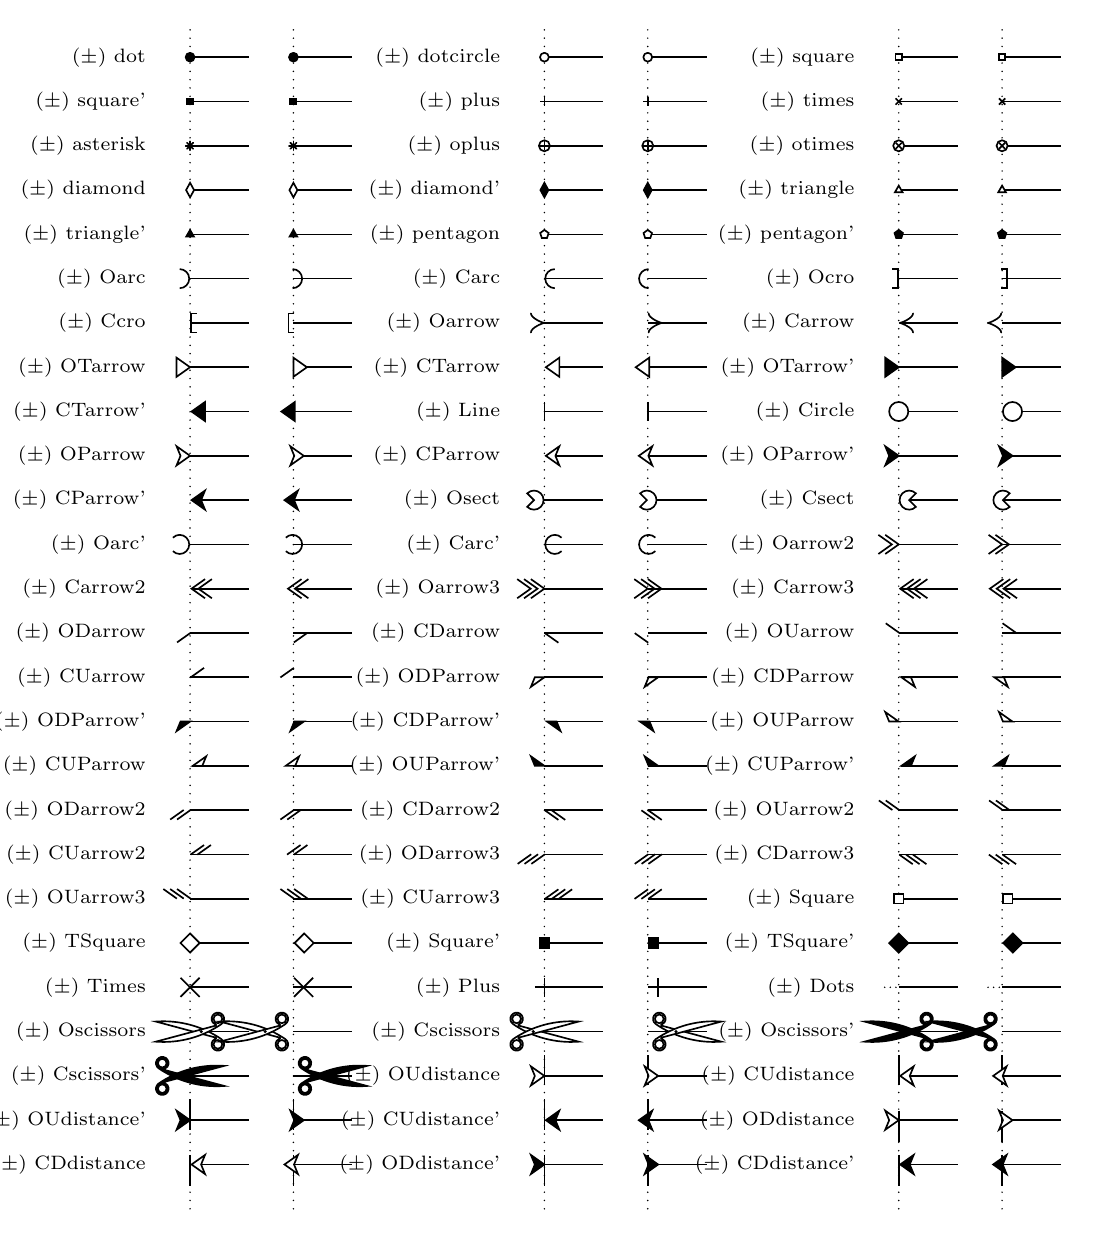
\begin{tikzpicture}%
\pgfsetxvec{\pgfxy(0.75,0)}%
\pgfsetyvec{\pgfxy(0,0.75)}%
\useasboundingbox (-6,-15)--(12,5);
%objet1  (User)
\pgfsetstrokecolor{rgb,1:red,0;green,0;blue,0}%
\pgfsetlinewidth{0.6pt}%
\pgfsetroundcap%
\pgfsetroundjoin%
\pgfsetdash{{0pt}{3pt}}{0pt}%
\pgfxyline(-3.25,-15)(-3.25,5)%
\pgfxyline(-1.5,-15)(-1.5,5)%
\pgfxyline(2.75,-15)(2.75,5)%
\pgfxyline(4.5,-15)(4.5,5)%
\pgfxyline(8.75,-15)(8.75,5)%
\pgfxyline(10.5,-15)(10.5,5)%
\pgfputat{\pgfxy(-4,4.5)}{\pgftext[right]{\color{rgb,1:red,0;green,0;blue,0}\scriptsize ($\pm$) dot}}\pgfstroke%
\pgfsetbuttcap%
\pgfsetdash{}{0pt}%
\pgfxyline(-3.25,4.5)(-2.25,4.5)%
\pgfsetroundcap%
\pgfpathmoveto{\pgfxy(-3.175,4.5)}\pgfellipse{\pgfxy(-3.25,4.5)}{\pgfxy(0.0000,0.075)}{\pgfxy(-0.075,0.0000)}%
\pgfsetfillcolor{rgb,1:red,0;green,0;blue,0}%
\pgffillstroke%
\pgfsetbuttcap%
\pgfxyline(-1.5,4.5)(-0.5,4.5)%
\pgfsetroundcap%
\pgfpathmoveto{\pgfxy(-1.425,4.5)}\pgfellipse{\pgfxy(-1.5,4.5)}{\pgfxy(0.0000,0.075)}{\pgfxy(-0.075,0.0000)}%
\pgfsetfillcolor{rgb,1:red,0;green,0;blue,0}%
\pgffillstroke%
\pgfputat{\pgfxy(2,4.5)}{\pgftext[right]{\color{rgb,1:red,0;green,0;blue,0}\scriptsize ($\pm$) dotcircle}}\pgfstroke%
\pgfsetbuttcap%
\pgfxyline(2.75,4.5)(3.75,4.5)%
\pgfsetroundcap%
\pgfpathmoveto{\pgfxy(2.825,4.5)}\pgfellipse{\pgfxy(2.75,4.5)}{\pgfxy(0.0000,0.075)}{\pgfxy(-0.075,0.0000)}%
\pgfsetfillcolor{rgb,1:red,1;green,1;blue,1}%
\pgffillstroke%
\pgfsetbuttcap%
\pgfxyline(4.5,4.5)(5.5,4.5)%
\pgfsetroundcap%
\pgfpathmoveto{\pgfxy(4.575,4.5)}\pgfellipse{\pgfxy(4.5,4.5)}{\pgfxy(0.0000,0.075)}{\pgfxy(-0.075,0.0000)}%
\pgfsetfillcolor{rgb,1:red,1;green,1;blue,1}%
\pgffillstroke%
\pgfputat{\pgfxy(8,4.5)}{\pgftext[right]{\color{rgb,1:red,0;green,0;blue,0}\scriptsize ($\pm$) square}}\pgfstroke%
\pgfsetbuttcap%
\pgfxyline(8.75,4.5)(9.75,4.5)%
\pgfsetmiterjoin%
\pgfpathmoveto{\pgfxy(8.803,4.553)}%
\pgfpathlineto{\pgfxy(8.697,4.553)}\pgfpathlineto{\pgfxy(8.697,4.447)}\pgfpathlineto{\pgfxy(8.803,4.447)}\pgfclosepath%
\pgfsetfillcolor{rgb,1:red,1;green,1;blue,1}%
\pgffillstroke%
\pgfsetroundjoin%
\pgfxyline(10.5,4.5)(11.5,4.5)%
\pgfsetmiterjoin%
\pgfpathmoveto{\pgfxy(10.553,4.553)}%
\pgfpathlineto{\pgfxy(10.447,4.553)}\pgfpathlineto{\pgfxy(10.447,4.447)}\pgfpathlineto{\pgfxy(10.553,4.447)}\pgfclosepath%
\pgfsetfillcolor{rgb,1:red,1;green,1;blue,1}%
\pgffillstroke%
\pgfputat{\pgfxy(-4,3.75)}{\pgftext[right]{\color{rgb,1:red,0;green,0;blue,0}\scriptsize ($\pm$) square'}}\pgfstroke%
\pgfsetroundjoin%
\pgfxyline(-3.25,3.75)(-2.25,3.75)%
\pgfsetmiterjoin%
\pgfpathmoveto{\pgfxy(-3.197,3.803)}%
\pgfpathlineto{\pgfxy(-3.303,3.803)}\pgfpathlineto{\pgfxy(-3.303,3.697)}\pgfpathlineto{\pgfxy(-3.197,3.697)}\pgfclosepath%
\pgfsetfillcolor{rgb,1:red,0;green,0;blue,0}%
\pgffillstroke%
\pgfsetroundjoin%
\pgfxyline(-1.5,3.75)(-0.5,3.75)%
\pgfsetmiterjoin%
\pgfpathmoveto{\pgfxy(-1.447,3.803)}%
\pgfpathlineto{\pgfxy(-1.553,3.803)}\pgfpathlineto{\pgfxy(-1.553,3.697)}\pgfpathlineto{\pgfxy(-1.447,3.697)}\pgfclosepath%
\pgfsetfillcolor{rgb,1:red,0;green,0;blue,0}%
\pgffillstroke%
\pgfputat{\pgfxy(2,3.75)}{\pgftext[right]{\color{rgb,1:red,0;green,0;blue,0}\scriptsize ($\pm$) plus}}\pgfstroke%
\pgfsetroundjoin%
\pgfxyline(2.75,3.75)(3.75,3.75)%
\pgfxyline(2.825,3.75)(2.675,3.75)%
\pgfxyline(2.75,3.825)(2.75,3.675)%
\pgfxyline(4.5,3.75)(5.5,3.75)%
\pgfxyline(4.575,3.75)(4.425,3.75)%
\pgfxyline(4.5,3.825)(4.5,3.675)%
\pgfputat{\pgfxy(8,3.75)}{\pgftext[right]{\color{rgb,1:red,0;green,0;blue,0}\scriptsize ($\pm$) times}}\pgfstroke%
\pgfxyline(8.75,3.75)(9.75,3.75)%
\pgfsetmiterjoin%
\pgfxyline(8.803,3.803)(8.697,3.697)%
\pgfxyline(8.697,3.803)(8.803,3.697)%
\pgfsetroundjoin%
\pgfxyline(10.5,3.75)(11.5,3.75)%
\pgfsetmiterjoin%
\pgfxyline(10.553,3.803)(10.447,3.697)%
\pgfxyline(10.447,3.803)(10.553,3.697)%
\pgfputat{\pgfxy(-4,3)}{\pgftext[right]{\color{rgb,1:red,0;green,0;blue,0}\scriptsize ($\pm$) asterisk}}\pgfstroke%
\pgfsetroundjoin%
\pgfxyline(-3.25,3)(-2.25,3)%
\pgfsetroundcap%
\pgfxyline(-3.175,3)(-3.325,3)%
\pgfxyline(-3.25,3.075)(-3.25,2.925)%
\pgfxyline(-3.197,3.053)(-3.303,2.947)%
\pgfxyline(-3.303,3.053)(-3.197,2.947)%
\pgfsetbuttcap%
\pgfxyline(-1.5,3)(-0.5,3)%
\pgfsetroundcap%
\pgfxyline(-1.425,3)(-1.575,3)%
\pgfxyline(-1.5,3.075)(-1.5,2.925)%
\pgfxyline(-1.447,3.053)(-1.553,2.947)%
\pgfxyline(-1.553,3.053)(-1.447,2.947)%
\pgfputat{\pgfxy(2,3)}{\pgftext[right]{\color{rgb,1:red,0;green,0;blue,0}\scriptsize ($\pm$) oplus}}\pgfstroke%
\pgfsetbuttcap%
\pgfxyline(2.75,3)(3.75,3)%
\pgfsetroundcap%
\pgfpathmoveto{\pgfxy(2.8437,3)}\pgfellipse{\pgfxy(2.75,3)}{\pgfxy(0.0000,0.0937)}{\pgfxy(-0.0937,0.0000)}%
\pgfsetfillcolor{rgb,1:red,1;green,1;blue,1}%
\pgffillstroke%
\pgfsetbuttcap%
\pgfxyline(2.825,3)(2.675,3)%
\pgfxyline(2.75,3.075)(2.75,2.925)%
\pgfxyline(4.5,3)(5.5,3)%
\pgfsetroundcap%
\pgfpathmoveto{\pgfxy(4.5937,3)}\pgfellipse{\pgfxy(4.5,3)}{\pgfxy(0.0000,0.0937)}{\pgfxy(-0.0937,0.0000)}%
\pgfsetfillcolor{rgb,1:red,1;green,1;blue,1}%
\pgffillstroke%
\pgfsetbuttcap%
\pgfxyline(4.575,3)(4.425,3)%
\pgfxyline(4.5,3.075)(4.5,2.925)%
\pgfputat{\pgfxy(8,3)}{\pgftext[right]{\color{rgb,1:red,0;green,0;blue,0}\scriptsize ($\pm$) otimes}}\pgfstroke%
\pgfxyline(8.75,3)(9.75,3)%
\pgfsetroundcap%
\pgfsetmiterjoin%
\pgfpathmoveto{\pgfxy(8.8437,3)}\pgfellipse{\pgfxy(8.75,3)}{\pgfxy(0.0000,0.0937)}{\pgfxy(-0.0937,0.0000)}%
\pgfsetfillcolor{rgb,1:red,1;green,1;blue,1}%
\pgffillstroke%
\pgfsetbuttcap%
\pgfxyline(8.803,3.053)(8.697,2.947)%
\pgfxyline(8.697,3.053)(8.803,2.947)%
\pgfsetroundjoin%
\pgfxyline(10.5,3)(11.5,3)%
\pgfsetroundcap%
\pgfsetmiterjoin%
\pgfpathmoveto{\pgfxy(10.5937,3)}\pgfellipse{\pgfxy(10.5,3)}{\pgfxy(0.0000,0.0937)}{\pgfxy(-0.0937,0.0000)}%
\pgfsetfillcolor{rgb,1:red,1;green,1;blue,1}%
\pgffillstroke%
\pgfsetbuttcap%
\pgfxyline(10.553,3.053)(10.447,2.947)%
\pgfxyline(10.447,3.053)(10.553,2.947)%
\pgfputat{\pgfxy(-4,2.25)}{\pgftext[right]{\color{rgb,1:red,0;green,0;blue,0}\scriptsize ($\pm$) diamond}}\pgfstroke%
\pgfsetroundjoin%
\pgfxyline(-3.25,2.25)(-2.25,2.25)%
\pgfsetmiterjoin%
\pgfpathmoveto{\pgfxy(-3.25,2.3737)}%
\pgfpathlineto{\pgfxy(-3.3175,2.25)}\pgfpathlineto{\pgfxy(-3.25,2.1263)}\pgfpathlineto{\pgfxy(-3.1825,2.25)}\pgfclosepath%
\pgfsetfillcolor{rgb,1:red,1;green,1;blue,1}%
\pgffillstroke%
\pgfsetroundjoin%
\pgfxyline(-1.5,2.25)(-0.5,2.25)%
\pgfsetmiterjoin%
\pgfpathmoveto{\pgfxy(-1.5,2.3737)}%
\pgfpathlineto{\pgfxy(-1.5675,2.25)}\pgfpathlineto{\pgfxy(-1.5,2.1263)}\pgfpathlineto{\pgfxy(-1.4325,2.25)}\pgfclosepath%
\pgfsetfillcolor{rgb,1:red,1;green,1;blue,1}%
\pgffillstroke%
\pgfputat{\pgfxy(2,2.25)}{\pgftext[right]{\color{rgb,1:red,0;green,0;blue,0}\scriptsize ($\pm$) diamond'}}\pgfstroke%
\pgfsetroundjoin%
\pgfxyline(2.75,2.25)(3.75,2.25)%
\pgfsetmiterjoin%
\pgfpathmoveto{\pgfxy(2.75,2.3737)}%
\pgfpathlineto{\pgfxy(2.6825,2.25)}\pgfpathlineto{\pgfxy(2.75,2.1263)}\pgfpathlineto{\pgfxy(2.8175,2.25)}\pgfclosepath%
\pgfsetfillcolor{rgb,1:red,0;green,0;blue,0}%
\pgffillstroke%
\pgfsetroundjoin%
\pgfxyline(4.5,2.25)(5.5,2.25)%
\pgfsetmiterjoin%
\pgfpathmoveto{\pgfxy(4.5,2.3737)}%
\pgfpathlineto{\pgfxy(4.4325,2.25)}\pgfpathlineto{\pgfxy(4.5,2.1263)}\pgfpathlineto{\pgfxy(4.5675,2.25)}\pgfclosepath%
\pgfsetfillcolor{rgb,1:red,0;green,0;blue,0}%
\pgffillstroke%
\pgfputat{\pgfxy(8,2.25)}{\pgftext[right]{\color{rgb,1:red,0;green,0;blue,0}\scriptsize ($\pm$) triangle}}\pgfstroke%
\pgfsetroundjoin%
\pgfxyline(8.75,2.25)(9.75,2.25)%
\pgfsetmiterjoin%
\pgfpathmoveto{\pgfxy(8.75,2.325)}%
\pgfpathlineto{\pgfxy(8.6851,2.2125)}\pgfpathlineto{\pgfxy(8.8149,2.2125)}\pgfclosepath%
\pgfsetfillcolor{rgb,1:red,1;green,1;blue,1}%
\pgffillstroke%
\pgfsetroundjoin%
\pgfxyline(10.5,2.25)(11.5,2.25)%
\pgfsetmiterjoin%
\pgfpathmoveto{\pgfxy(10.5,2.325)}%
\pgfpathlineto{\pgfxy(10.4351,2.2125)}\pgfpathlineto{\pgfxy(10.5649,2.2125)}\pgfclosepath%
\pgfsetfillcolor{rgb,1:red,1;green,1;blue,1}%
\pgffillstroke%
\pgfputat{\pgfxy(-4,1.5)}{\pgftext[right]{\color{rgb,1:red,0;green,0;blue,0}\scriptsize ($\pm$) triangle'}}\pgfstroke%
\pgfsetroundjoin%
\pgfxyline(-3.25,1.5)(-2.25,1.5)%
\pgfsetmiterjoin%
\pgfpathmoveto{\pgfxy(-3.25,1.575)}%
\pgfpathlineto{\pgfxy(-3.3149,1.4625)}\pgfpathlineto{\pgfxy(-3.1851,1.4625)}\pgfclosepath%
\pgfsetfillcolor{rgb,1:red,0;green,0;blue,0}%
\pgffillstroke%
\pgfsetroundjoin%
\pgfxyline(-1.5,1.5)(-0.5,1.5)%
\pgfsetmiterjoin%
\pgfpathmoveto{\pgfxy(-1.5,1.575)}%
\pgfpathlineto{\pgfxy(-1.5649,1.4625)}\pgfpathlineto{\pgfxy(-1.4351,1.4625)}\pgfclosepath%
\pgfsetfillcolor{rgb,1:red,0;green,0;blue,0}%
\pgffillstroke%
\pgfputat{\pgfxy(2,1.5)}{\pgftext[right]{\color{rgb,1:red,0;green,0;blue,0}\scriptsize ($\pm$) pentagon}}\pgfstroke%
\pgfsetroundjoin%
\pgfxyline(2.75,1.5)(3.75,1.5)%
\pgfsetmiterjoin%
\pgfpathmoveto{\pgfxy(2.75,1.575)}%
\pgfpathlineto{\pgfxy(2.6787,1.5232)}\pgfpathlineto{\pgfxy(2.7059,1.4393)}\pgfpathlineto{\pgfxy(2.7941,1.4393)}\pgfpathlineto{\pgfxy(2.8213,1.5232)}%
\pgfclosepath%
\pgfsetfillcolor{rgb,1:red,1;green,1;blue,1}%
\pgffillstroke%
\pgfsetroundjoin%
\pgfxyline(4.5,1.5)(5.5,1.5)%
\pgfsetmiterjoin%
\pgfpathmoveto{\pgfxy(4.5,1.575)}%
\pgfpathlineto{\pgfxy(4.4287,1.5232)}\pgfpathlineto{\pgfxy(4.4559,1.4393)}\pgfpathlineto{\pgfxy(4.5441,1.4393)}\pgfpathlineto{\pgfxy(4.5713,1.5232)}%
\pgfclosepath%
\pgfsetfillcolor{rgb,1:red,1;green,1;blue,1}%
\pgffillstroke%
\pgfputat{\pgfxy(8,1.5)}{\pgftext[right]{\color{rgb,1:red,0;green,0;blue,0}\scriptsize ($\pm$) pentagon'}}\pgfstroke%
\pgfsetroundjoin%
\pgfxyline(8.75,1.5)(9.75,1.5)%
\pgfsetmiterjoin%
\pgfpathmoveto{\pgfxy(8.75,1.575)}%
\pgfpathlineto{\pgfxy(8.6787,1.5232)}\pgfpathlineto{\pgfxy(8.7059,1.4393)}\pgfpathlineto{\pgfxy(8.7941,1.4393)}\pgfpathlineto{\pgfxy(8.8213,1.5232)}%
\pgfclosepath%
\pgfsetfillcolor{rgb,1:red,0;green,0;blue,0}%
\pgffillstroke%
\pgfsetroundjoin%
\pgfxyline(10.5,1.5)(11.5,1.5)%
\pgfsetmiterjoin%
\pgfpathmoveto{\pgfxy(10.5,1.575)}%
\pgfpathlineto{\pgfxy(10.4287,1.5232)}\pgfpathlineto{\pgfxy(10.4559,1.4393)}\pgfpathlineto{\pgfxy(10.5441,1.4393)}\pgfpathlineto{\pgfxy(10.5713,1.5232)}%
\pgfclosepath%
\pgfsetfillcolor{rgb,1:red,0;green,0;blue,0}%
\pgffillstroke%
\pgfputat{\pgfxy(-4,0.75)}{\pgftext[right]{\color{rgb,1:red,0;green,0;blue,0}\scriptsize ($\pm$) Oarc}}\pgfstroke%
\pgfsetroundjoin%
\pgfxyline(-3.25,0.75)(-2.25,0.75)%
\pgfpathmoveto{\pgfxy(-3.4262,0.5881)}\pgfpatharc{-90}{90}{0.1214cm}%
\pgfstroke%
\pgfxyline(-1.5,0.75)(-0.5,0.75)%
\pgfpathmoveto{\pgfxy(-1.5143,0.5881)}\pgfpatharc{-90}{90}{0.1214cm}%
\pgfstroke%
\pgfputat{\pgfxy(2,0.75)}{\pgftext[right]{\color{rgb,1:red,0;green,0;blue,0}\scriptsize ($\pm$) Carc}}\pgfstroke%
\pgfxyline(2.75,0.75)(3.75,0.75)%
\pgfpathmoveto{\pgfxy(2.9262,0.9119)}\pgfpatharc{90}{270}{0.1214cm}%
\pgfstroke%
\pgfxyline(4.5,0.75)(5.5,0.75)%
\pgfpathmoveto{\pgfxy(4.5143,0.9119)}\pgfpatharc{90}{270}{0.1214cm}%
\pgfstroke%
\pgfputat{\pgfxy(8,0.75)}{\pgftext[right]{\color{rgb,1:red,0;green,0;blue,0}\scriptsize ($\pm$) Ocro}}\pgfstroke%
\pgfxyline(8.75,0.75)(9.75,0.75)%
\pgfsetmiterjoin%
\pgfpathmoveto{\pgfxy(8.6405,0.9119)}%
\pgfpathlineto{\pgfxy(8.7357,0.9119)}\pgfpathlineto{\pgfxy(8.7357,0.5881)}\pgfpathlineto{\pgfxy(8.6405,0.5881)}%
\pgfstroke%
\pgfsetroundjoin%
\pgfxyline(10.5,0.75)(11.5,0.75)%
\pgfsetmiterjoin%
\pgfpathmoveto{\pgfxy(10.4857,0.9119)}%
\pgfpathlineto{\pgfxy(10.581,0.9119)}\pgfpathlineto{\pgfxy(10.581,0.5881)}\pgfpathlineto{\pgfxy(10.4857,0.5881)}%
\pgfstroke%
\pgfputat{\pgfxy(-4,0)}{\pgftext[right]{\color{rgb,1:red,0;green,0;blue,0}\scriptsize ($\pm$) Ccro}}\pgfstroke%
\pgfsetroundjoin%
\pgfxyline(-3.25,0)(-2.25,0)%
\pgfsetmiterjoin%
\pgfpathmoveto{\pgfxy(-3.1405,0.1619)}%
\pgfpathlineto{\pgfxy(-3.2357,0.1619)}\pgfpathlineto{\pgfxy(-3.2357,-0.1619)}\pgfpathlineto{\pgfxy(-3.1405,-0.1619)}%
\pgfstroke%
\pgfsetroundjoin%
\pgfxyline(-1.5,0)(-0.5,0)%
\pgfsetmiterjoin%
\pgfpathmoveto{\pgfxy(-1.4857,0.1619)}%
\pgfpathlineto{\pgfxy(-1.581,0.1619)}\pgfpathlineto{\pgfxy(-1.581,-0.1619)}\pgfpathlineto{\pgfxy(-1.4857,-0.1619)}%
\pgfstroke%
\pgfputat{\pgfxy(2,0)}{\pgftext[right]{\color{rgb,1:red,0;green,0;blue,0}\scriptsize ($\pm$) Oarrow}}\pgfstroke%
\pgfsetroundjoin%
\pgfxyline(2.75,0)(3.75,0)%
\pgfsetroundcap%
\pgfpathmoveto{\pgfxy(2.5214,-0.1619)}%
\pgfpathcurveto{\pgfxy(2.5214,-0.081)}{\pgfxy(2.7214,0)}{\pgfxy(2.75,0)}%
\pgfpathcurveto{\pgfxy(2.7214,0)}{\pgfxy(2.5214,0.081)}{\pgfxy(2.5214,0.1619)}%
\pgfstroke%
\pgfsetbuttcap%
\pgfxyline(4.5,0)(5.5,0)%
\pgfsetroundcap%
\pgfpathmoveto{\pgfxy(4.5143,-0.1619)}%
\pgfpathcurveto{\pgfxy(4.5143,-0.081)}{\pgfxy(4.7143,0)}{\pgfxy(4.7429,0)}%
\pgfpathcurveto{\pgfxy(4.7143,0)}{\pgfxy(4.5143,0.081)}{\pgfxy(4.5143,0.1619)}%
\pgfstroke%
\pgfputat{\pgfxy(8,0)}{\pgftext[right]{\color{rgb,1:red,0;green,0;blue,0}\scriptsize ($\pm$) Carrow}}\pgfstroke%
\pgfsetbuttcap%
\pgfxyline(8.7908,0)(9.75,0)%
\pgfsetroundcap%
\pgfpathmoveto{\pgfxy(8.9929,-0.1619)}%
\pgfpathcurveto{\pgfxy(8.9929,-0.081)}{\pgfxy(8.7929,0)}{\pgfxy(8.7643,0)}%
\pgfpathcurveto{\pgfxy(8.7929,0)}{\pgfxy(8.9929,0.081)}{\pgfxy(8.9929,0.1619)}%
\pgfstroke%
\pgfsetbuttcap%
\pgfxyline(10.5,0)(11.5,0)%
\pgfsetroundcap%
\pgfpathmoveto{\pgfxy(10.4857,-0.1619)}%
\pgfpathcurveto{\pgfxy(10.4857,-0.081)}{\pgfxy(10.2857,0)}{\pgfxy(10.2571,0)}%
\pgfpathcurveto{\pgfxy(10.2857,0)}{\pgfxy(10.4857,0.081)}{\pgfxy(10.4857,0.1619)}%
\pgfstroke%
\pgfputat{\pgfxy(-4,-0.75)}{\pgftext[right]{\color{rgb,1:red,0;green,0;blue,0}\scriptsize ($\pm$) OTarrow}}\pgfstroke%
\pgfsetbuttcap%
\pgfxyline(-3.25,-0.75)(-2.25,-0.75)%
\pgfsetmiterjoin%
\pgfpathmoveto{\pgfxy(-3.25,-0.75)}%
\pgfpathlineto{\pgfxy(-3.4786,-0.5881)}\pgfpathlineto{\pgfxy(-3.4786,-0.9119)}\pgfclosepath%
\pgfsetfillcolor{rgb,1:red,1;green,1;blue,1}%
\pgffillstroke%
\pgfsetroundjoin%
\pgfxyline(-1.5,-0.75)(-0.5,-0.75)%
\pgfsetmiterjoin%
\pgfpathmoveto{\pgfxy(-1.2714,-0.75)}%
\pgfpathlineto{\pgfxy(-1.5,-0.5881)}\pgfpathlineto{\pgfxy(-1.5,-0.9119)}\pgfclosepath%
\pgfsetfillcolor{rgb,1:red,1;green,1;blue,1}%
\pgffillstroke%
\pgfputat{\pgfxy(2,-0.75)}{\pgftext[right]{\color{rgb,1:red,0;green,0;blue,0}\scriptsize ($\pm$) CTarrow}}\pgfstroke%
\pgfsetroundjoin%
\pgfxyline(2.7908,-0.75)(3.75,-0.75)%
\pgfsetmiterjoin%
\pgfpathmoveto{\pgfxy(2.7747,-0.75)}%
\pgfpathlineto{\pgfxy(3.0033,-0.5881)}\pgfpathlineto{\pgfxy(3.0033,-0.9119)}\pgfclosepath%
\pgfsetfillcolor{rgb,1:red,1;green,1;blue,1}%
\pgffillstroke%
\pgfsetroundjoin%
\pgfxyline(4.5,-0.75)(5.5,-0.75)%
\pgfsetmiterjoin%
\pgfpathmoveto{\pgfxy(4.2961,-0.75)}%
\pgfpathlineto{\pgfxy(4.5247,-0.5881)}\pgfpathlineto{\pgfxy(4.5247,-0.9119)}\pgfclosepath%
\pgfsetfillcolor{rgb,1:red,1;green,1;blue,1}%
\pgffillstroke%
\pgfputat{\pgfxy(8,-0.75)}{\pgftext[right]{\color{rgb,1:red,0;green,0;blue,0}\scriptsize ($\pm$) OTarrow'}}\pgfstroke%
\pgfsetroundjoin%
\pgfxyline(8.75,-0.75)(9.75,-0.75)%
\pgfsetmiterjoin%
\pgfpathmoveto{\pgfxy(8.75,-0.75)}%
\pgfpathlineto{\pgfxy(8.5214,-0.5881)}\pgfpathlineto{\pgfxy(8.5214,-0.9119)}\pgfclosepath%
\pgfsetfillcolor{rgb,1:red,0;green,0;blue,0}%
\pgffillstroke%
\pgfsetroundjoin%
\pgfxyline(10.5,-0.75)(11.5,-0.75)%
\pgfsetmiterjoin%
\pgfpathmoveto{\pgfxy(10.7286,-0.75)}%
\pgfpathlineto{\pgfxy(10.5,-0.5881)}\pgfpathlineto{\pgfxy(10.5,-0.9119)}\pgfclosepath%
\pgfsetfillcolor{rgb,1:red,0;green,0;blue,0}%
\pgffillstroke%
\pgfputat{\pgfxy(-4,-1.5)}{\pgftext[right]{\color{rgb,1:red,0;green,0;blue,0}\scriptsize ($\pm$) CTarrow'}}\pgfstroke%
\pgfsetroundjoin%
\pgfxyline(-3.2092,-1.5)(-2.25,-1.5)%
\pgfsetmiterjoin%
\pgfpathmoveto{\pgfxy(-3.2253,-1.5)}%
\pgfpathlineto{\pgfxy(-2.9967,-1.3381)}\pgfpathlineto{\pgfxy(-2.9967,-1.6619)}\pgfclosepath%
\pgfsetfillcolor{rgb,1:red,0;green,0;blue,0}%
\pgffillstroke%
\pgfsetroundjoin%
\pgfxyline(-1.5,-1.5)(-0.5,-1.5)%
\pgfsetmiterjoin%
\pgfpathmoveto{\pgfxy(-1.7039,-1.5)}%
\pgfpathlineto{\pgfxy(-1.4753,-1.3381)}\pgfpathlineto{\pgfxy(-1.4753,-1.6619)}\pgfclosepath%
\pgfsetfillcolor{rgb,1:red,0;green,0;blue,0}%
\pgffillstroke%
\pgfputat{\pgfxy(2,-1.5)}{\pgftext[right]{\color{rgb,1:red,0;green,0;blue,0}\scriptsize ($\pm$) Line}}\pgfstroke%
\pgfsetroundjoin%
\pgfxyline(2.75,-1.5)(3.75,-1.5)%
\pgfxyline(2.75,-1.3381)(2.75,-1.6619)%
\pgfxyline(4.5,-1.5)(5.5,-1.5)%
\pgfxyline(4.5,-1.3381)(4.5,-1.6619)%
\pgfputat{\pgfxy(8,-1.5)}{\pgftext[right]{\color{rgb,1:red,0;green,0;blue,0}\scriptsize ($\pm$) Circle}}\pgfstroke%
\pgfxyline(8.75,-1.5)(9.75,-1.5)%
\pgfellipse{\pgfxy(8.75,-1.5)}{\pgfxy(0.0000,0.1619)}{\pgfxy(-0.1619,0.0000)}%
\pgfsetfillcolor{rgb,1:red,1;green,1;blue,1}%
\pgffillstroke%
\pgfxyline(10.5408,-1.5)(11.5,-1.5)%
\pgfellipse{\pgfxy(10.6762,-1.5)}{\pgfxy(0.0000,0.1619)}{\pgfxy(-0.1619,0.0000)}%
\pgfsetfillcolor{rgb,1:red,1;green,1;blue,1}%
\pgffillstroke%
\pgfputat{\pgfxy(-4,-2.25)}{\pgftext[right]{\color{rgb,1:red,0;green,0;blue,0}\scriptsize ($\pm$) OParrow}}\pgfstroke%
\pgfxyline(-3.25,-2.25)(-2.25,-2.25)%
\pgfsetmiterjoin%
\pgfpathmoveto{\pgfxy(-3.25,-2.25)}%
\pgfpathlineto{\pgfxy(-3.4786,-2.4119)}\pgfpathlineto{\pgfxy(-3.4119,-2.25)}\pgfpathlineto{\pgfxy(-3.4786,-2.0881)}\pgfclosepath%
\pgfsetfillcolor{rgb,1:red,1;green,1;blue,1}%
\pgffillstroke%
\pgfsetroundjoin%
\pgfxyline(-1.5,-2.25)(-0.5,-2.25)%
\pgfsetmiterjoin%
\pgfpathmoveto{\pgfxy(-1.3238,-2.25)}%
\pgfpathlineto{\pgfxy(-1.5524,-2.4119)}\pgfpathlineto{\pgfxy(-1.4857,-2.25)}\pgfpathlineto{\pgfxy(-1.5524,-2.0881)}\pgfclosepath%
\pgfsetfillcolor{rgb,1:red,1;green,1;blue,1}%
\pgffillstroke%
\pgfputat{\pgfxy(2,-2.25)}{\pgftext[right]{\color{rgb,1:red,0;green,0;blue,0}\scriptsize ($\pm$) CParrow}}\pgfstroke%
\pgfsetroundjoin%
\pgfxyline(2.7908,-2.25)(3.75,-2.25)%
\pgfsetmiterjoin%
\pgfpathmoveto{\pgfxy(2.7747,-2.25)}%
\pgfpathlineto{\pgfxy(3.0033,-2.4119)}\pgfpathlineto{\pgfxy(2.9366,-2.25)}\pgfpathlineto{\pgfxy(3.0033,-2.0881)}\pgfclosepath%
\pgfsetfillcolor{rgb,1:red,1;green,1;blue,1}%
\pgffillstroke%
\pgfsetroundjoin%
\pgfxyline(4.5,-2.25)(5.5,-2.25)%
\pgfsetmiterjoin%
\pgfpathmoveto{\pgfxy(4.3485,-2.25)}%
\pgfpathlineto{\pgfxy(4.5771,-2.4119)}\pgfpathlineto{\pgfxy(4.5104,-2.25)}\pgfpathlineto{\pgfxy(4.5771,-2.0881)}\pgfclosepath%
\pgfsetfillcolor{rgb,1:red,1;green,1;blue,1}%
\pgffillstroke%
\pgfputat{\pgfxy(8,-2.25)}{\pgftext[right]{\color{rgb,1:red,0;green,0;blue,0}\scriptsize ($\pm$) OParrow'}}\pgfstroke%
\pgfsetroundjoin%
\pgfxyline(8.75,-2.25)(9.75,-2.25)%
\pgfsetmiterjoin%
\pgfpathmoveto{\pgfxy(8.75,-2.25)}%
\pgfpathlineto{\pgfxy(8.5214,-2.4119)}\pgfpathlineto{\pgfxy(8.5881,-2.25)}\pgfpathlineto{\pgfxy(8.5214,-2.0881)}\pgfclosepath%
\pgfsetfillcolor{rgb,1:red,0;green,0;blue,0}%
\pgffillstroke%
\pgfsetroundjoin%
\pgfxyline(10.5,-2.25)(11.5,-2.25)%
\pgfsetmiterjoin%
\pgfpathmoveto{\pgfxy(10.6762,-2.25)}%
\pgfpathlineto{\pgfxy(10.4476,-2.4119)}\pgfpathlineto{\pgfxy(10.5143,-2.25)}\pgfpathlineto{\pgfxy(10.4476,-2.0881)}\pgfclosepath%
\pgfsetfillcolor{rgb,1:red,0;green,0;blue,0}%
\pgffillstroke%
\pgfputat{\pgfxy(-4,-3)}{\pgftext[right]{\color{rgb,1:red,0;green,0;blue,0}\scriptsize ($\pm$) CParrow'}}\pgfstroke%
\pgfsetroundjoin%
\pgfxyline(-3.2092,-3)(-2.25,-3)%
\pgfsetmiterjoin%
\pgfpathmoveto{\pgfxy(-3.2253,-3)}%
\pgfpathlineto{\pgfxy(-2.9967,-3.1619)}\pgfpathlineto{\pgfxy(-3.0634,-3)}\pgfpathlineto{\pgfxy(-2.9967,-2.8381)}\pgfclosepath%
\pgfsetfillcolor{rgb,1:red,0;green,0;blue,0}%
\pgffillstroke%
\pgfsetroundjoin%
\pgfxyline(-1.5,-3)(-0.5,-3)%
\pgfsetmiterjoin%
\pgfpathmoveto{\pgfxy(-1.6515,-3)}%
\pgfpathlineto{\pgfxy(-1.4229,-3.1619)}\pgfpathlineto{\pgfxy(-1.4896,-3)}\pgfpathlineto{\pgfxy(-1.4229,-2.8381)}\pgfclosepath%
\pgfsetfillcolor{rgb,1:red,0;green,0;blue,0}%
\pgffillstroke%
\pgfputat{\pgfxy(2,-3)}{\pgftext[right]{\color{rgb,1:red,0;green,0;blue,0}\scriptsize ($\pm$) Osect}}\pgfstroke%
\pgfsetroundjoin%
\pgfxyline(2.75,-3)(3.75,-3)%
\pgfsetmiterjoin%
\pgfpathmoveto{\pgfxy(2.4593,-3.1145)}\pgfpatharc{-135}{135}{0.1214cm}%
\pgfpathlineto{\pgfxy(2.5738,-3)}%
\pgfclosepath%
\pgfsetfillcolor{rgb,1:red,1;green,1;blue,1}%
\pgffillstroke%
\pgfsetroundjoin%
\pgfxyline(4.5,-3)(5.5,-3)%
\pgfsetmiterjoin%
\pgfpathmoveto{\pgfxy(4.3712,-3.1145)}\pgfpatharc{-135}{135}{0.1214cm}%
\pgfpathlineto{\pgfxy(4.4857,-3)}%
\pgfclosepath%
\pgfsetfillcolor{rgb,1:red,1;green,1;blue,1}%
\pgffillstroke%
\pgfputat{\pgfxy(8,-3)}{\pgftext[right]{\color{rgb,1:red,0;green,0;blue,0}\scriptsize ($\pm$) Csect}}\pgfstroke%
\pgfsetroundjoin%
\pgfxyline(8.7908,-3)(9.75,-3)%
\pgfsetmiterjoin%
\pgfpathmoveto{\pgfxy(9.0407,-2.8855)}\pgfpatharc{45}{315}{0.1214cm}%
\pgfpathlineto{\pgfxy(8.9262,-3)}%
\pgfclosepath%
\pgfsetfillcolor{rgb,1:red,1;green,1;blue,1}%
\pgffillstroke%
\pgfsetroundjoin%
\pgfxyline(10.5,-3)(11.5,-3)%
\pgfsetmiterjoin%
\pgfpathmoveto{\pgfxy(10.6288,-2.8855)}\pgfpatharc{45}{315}{0.1214cm}%
\pgfpathlineto{\pgfxy(10.5143,-3)}%
\pgfclosepath%
\pgfsetfillcolor{rgb,1:red,1;green,1;blue,1}%
\pgffillstroke%
\pgfputat{\pgfxy(-4,-3.75)}{\pgftext[right]{\color{rgb,1:red,0;green,0;blue,0}\scriptsize ($\pm$) Oarc'}}\pgfstroke%
\pgfsetroundjoin%
\pgfxyline(-3.25,-3.75)(-2.25,-3.75)%
\pgfpathmoveto{\pgfxy(-3.5407,-3.8645)}\pgfpatharc{-135}{135}{0.1214cm}%
\pgfstroke%
\pgfxyline(-1.5,-3.75)(-0.5,-3.75)%
\pgfpathmoveto{\pgfxy(-1.6288,-3.8645)}\pgfpatharc{-135}{135}{0.1214cm}%
\pgfstroke%
\pgfputat{\pgfxy(2,-3.75)}{\pgftext[right]{\color{rgb,1:red,0;green,0;blue,0}\scriptsize ($\pm$) Carc'}}\pgfstroke%
\pgfxyline(2.75,-3.75)(3.75,-3.75)%
\pgfpathmoveto{\pgfxy(3.0407,-3.6355)}\pgfpatharc{45}{315}{0.1214cm}%
\pgfstroke%
\pgfxyline(4.5,-3.75)(5.5,-3.75)%
\pgfpathmoveto{\pgfxy(4.6288,-3.6355)}\pgfpatharc{45}{315}{0.1214cm}%
\pgfstroke%
\pgfputat{\pgfxy(8,-3.75)}{\pgftext[right]{\color{rgb,1:red,0;green,0;blue,0}\scriptsize ($\pm$) Oarrow2}}\pgfstroke%
\pgfxyline(8.75,-3.75)(9.75,-3.75)%
\pgfsetmiterjoin%
\pgfpathmoveto{\pgfxy(8.5214,-3.9119)}%
\pgfpathlineto{\pgfxy(8.75,-3.75)}\pgfpathlineto{\pgfxy(8.5214,-3.5881)}%
\pgfstroke%
\pgfpathmoveto{\pgfxy(8.4053,-3.9119)}%
\pgfpathlineto{\pgfxy(8.6339,-3.75)}\pgfpathlineto{\pgfxy(8.4053,-3.5881)}%
\pgfstroke%
\pgfsetroundjoin%
\pgfxyline(10.5,-3.75)(11.5,-3.75)%
\pgfsetmiterjoin%
\pgfpathmoveto{\pgfxy(10.3875,-3.9119)}%
\pgfpathlineto{\pgfxy(10.6161,-3.75)}\pgfpathlineto{\pgfxy(10.3875,-3.5881)}%
\pgfstroke%
\pgfpathmoveto{\pgfxy(10.2714,-3.9119)}%
\pgfpathlineto{\pgfxy(10.5,-3.75)}\pgfpathlineto{\pgfxy(10.2714,-3.5881)}%
\pgfstroke%
\pgfputat{\pgfxy(-4,-4.5)}{\pgftext[right]{\color{rgb,1:red,0;green,0;blue,0}\scriptsize ($\pm$) Carrow2}}\pgfstroke%
\pgfsetroundjoin%
\pgfxyline(-3.2092,-4.5)(-2.25,-4.5)%
\pgfsetmiterjoin%
\pgfpathmoveto{\pgfxy(-2.9967,-4.6619)}%
\pgfpathlineto{\pgfxy(-3.2253,-4.5)}\pgfpathlineto{\pgfxy(-2.9967,-4.3381)}%
\pgfstroke%
\pgfpathmoveto{\pgfxy(-2.8806,-4.6619)}%
\pgfpathlineto{\pgfxy(-3.1092,-4.5)}\pgfpathlineto{\pgfxy(-2.8806,-4.3381)}%
\pgfstroke%
\pgfsetroundjoin%
\pgfxyline(-1.4592,-4.5)(-0.5,-4.5)%
\pgfsetmiterjoin%
\pgfpathmoveto{\pgfxy(-1.3628,-4.6619)}%
\pgfpathlineto{\pgfxy(-1.5914,-4.5)}\pgfpathlineto{\pgfxy(-1.3628,-4.3381)}%
\pgfstroke%
\pgfpathmoveto{\pgfxy(-1.2467,-4.6619)}%
\pgfpathlineto{\pgfxy(-1.4753,-4.5)}\pgfpathlineto{\pgfxy(-1.2467,-4.3381)}%
\pgfstroke%
\pgfputat{\pgfxy(2,-4.5)}{\pgftext[right]{\color{rgb,1:red,0;green,0;blue,0}\scriptsize ($\pm$) Oarrow3}}\pgfstroke%
\pgfsetroundjoin%
\pgfxyline(2.75,-4.5)(3.75,-4.5)%
\pgfsetmiterjoin%
\pgfpathmoveto{\pgfxy(2.5214,-4.6619)}%
\pgfpathlineto{\pgfxy(2.75,-4.5)}\pgfpathlineto{\pgfxy(2.5214,-4.3381)}%
\pgfstroke%
\pgfpathmoveto{\pgfxy(2.4053,-4.6619)}%
\pgfpathlineto{\pgfxy(2.6339,-4.5)}\pgfpathlineto{\pgfxy(2.4053,-4.3381)}%
\pgfstroke%
\pgfpathmoveto{\pgfxy(2.2892,-4.6619)}%
\pgfpathlineto{\pgfxy(2.5178,-4.5)}\pgfpathlineto{\pgfxy(2.2892,-4.3381)}%
\pgfstroke%
\pgfsetroundjoin%
\pgfxyline(4.5,-4.5)(5.5,-4.5)%
\pgfsetmiterjoin%
\pgfpathmoveto{\pgfxy(4.5036,-4.6619)}%
\pgfpathlineto{\pgfxy(4.7322,-4.5)}\pgfpathlineto{\pgfxy(4.5036,-4.3381)}%
\pgfstroke%
\pgfpathmoveto{\pgfxy(4.3875,-4.6619)}%
\pgfpathlineto{\pgfxy(4.6161,-4.5)}\pgfpathlineto{\pgfxy(4.3875,-4.3381)}%
\pgfstroke%
\pgfpathmoveto{\pgfxy(4.2714,-4.6619)}%
\pgfpathlineto{\pgfxy(4.5,-4.5)}\pgfpathlineto{\pgfxy(4.2714,-4.3381)}%
\pgfstroke%
\pgfputat{\pgfxy(8,-4.5)}{\pgftext[right]{\color{rgb,1:red,0;green,0;blue,0}\scriptsize ($\pm$) Carrow3}}\pgfstroke%
\pgfsetroundjoin%
\pgfxyline(8.7908,-4.5)(9.75,-4.5)%
\pgfsetmiterjoin%
\pgfpathmoveto{\pgfxy(9.0033,-4.6619)}%
\pgfpathlineto{\pgfxy(8.7747,-4.5)}\pgfpathlineto{\pgfxy(9.0033,-4.3381)}%
\pgfstroke%
\pgfpathmoveto{\pgfxy(9.1194,-4.6619)}%
\pgfpathlineto{\pgfxy(8.8908,-4.5)}\pgfpathlineto{\pgfxy(9.1194,-4.3381)}%
\pgfstroke%
\pgfpathmoveto{\pgfxy(9.2355,-4.6619)}%
\pgfpathlineto{\pgfxy(9.0069,-4.5)}\pgfpathlineto{\pgfxy(9.2355,-4.3381)}%
\pgfstroke%
\pgfsetroundjoin%
\pgfxyline(10.5408,-4.5)(11.5,-4.5)%
\pgfsetmiterjoin%
\pgfpathmoveto{\pgfxy(10.5211,-4.6619)}%
\pgfpathlineto{\pgfxy(10.2925,-4.5)}\pgfpathlineto{\pgfxy(10.5211,-4.3381)}%
\pgfstroke%
\pgfpathmoveto{\pgfxy(10.6372,-4.6619)}%
\pgfpathlineto{\pgfxy(10.4086,-4.5)}\pgfpathlineto{\pgfxy(10.6372,-4.3381)}%
\pgfstroke%
\pgfpathmoveto{\pgfxy(10.7533,-4.6619)}%
\pgfpathlineto{\pgfxy(10.5247,-4.5)}\pgfpathlineto{\pgfxy(10.7533,-4.3381)}%
\pgfstroke%
\pgfputat{\pgfxy(-4,-5.25)}{\pgftext[right]{\color{rgb,1:red,0;green,0;blue,0}\scriptsize ($\pm$) ODarrow}}\pgfstroke%
\pgfsetroundjoin%
\pgfxyline(-3.25,-5.25)(-2.25,-5.25)%
\pgfsetmiterjoin%
\pgfxyline(-3.2417,-5.2474)(-3.4703,-5.4093)%
\pgfsetroundjoin%
\pgfxyline(-1.5,-5.25)(-0.5,-5.25)%
\pgfsetmiterjoin%
\pgfxyline(-1.2632,-5.2474)(-1.4917,-5.4093)%
\pgfputat{\pgfxy(2,-5.25)}{\pgftext[right]{\color{rgb,1:red,0;green,0;blue,0}\scriptsize ($\pm$) CDarrow}}\pgfstroke%
\pgfsetroundjoin%
\pgfxyline(2.75,-5.25)(3.75,-5.25)%
\pgfsetmiterjoin%
\pgfxyline(2.7583,-5.2526)(2.9868,-5.4145)%
\pgfsetroundjoin%
\pgfxyline(4.5,-5.25)(5.5,-5.25)%
\pgfsetmiterjoin%
\pgfxyline(4.2797,-5.2526)(4.5083,-5.4145)%
\pgfputat{\pgfxy(8,-5.25)}{\pgftext[right]{\color{rgb,1:red,0;green,0;blue,0}\scriptsize ($\pm$) OUarrow}}\pgfstroke%
\pgfsetroundjoin%
\pgfxyline(8.75,-5.25)(9.75,-5.25)%
\pgfsetmiterjoin%
\pgfxyline(8.7583,-5.2474)(8.5297,-5.0855)%
\pgfsetroundjoin%
\pgfxyline(10.5,-5.25)(11.5,-5.25)%
\pgfsetmiterjoin%
\pgfxyline(10.7368,-5.2474)(10.5083,-5.0855)%
\pgfputat{\pgfxy(-4,-6)}{\pgftext[right]{\color{rgb,1:red,0;green,0;blue,0}\scriptsize ($\pm$) CUarrow}}\pgfstroke%
\pgfsetroundjoin%
\pgfxyline(-3.25,-6)(-2.25,-6)%
\pgfsetmiterjoin%
\pgfxyline(-3.2417,-6.0026)(-3.0132,-5.8407)%
\pgfsetroundjoin%
\pgfxyline(-1.5,-6)(-0.5,-6)%
\pgfsetmiterjoin%
\pgfxyline(-1.7203,-6.0026)(-1.4917,-5.8407)%
\pgfputat{\pgfxy(2,-6)}{\pgftext[right]{\color{rgb,1:red,0;green,0;blue,0}\scriptsize ($\pm$) ODParrow}}\pgfstroke%
\pgfsetroundjoin%
\pgfxyline(2.75,-6)(3.75,-6)%
\pgfsetmiterjoin%
\pgfpathmoveto{\pgfxy(2.75,-6)}%
\pgfpathlineto{\pgfxy(2.5881,-6)}\pgfpathlineto{\pgfxy(2.5214,-6.1619)}\pgfclosepath%
\pgfsetfillcolor{rgb,1:red,1;green,1;blue,1}%
\pgffillstroke%
\pgfsetroundjoin%
\pgfxyline(4.5,-6)(5.5,-6)%
\pgfsetmiterjoin%
\pgfpathmoveto{\pgfxy(4.6762,-6)}%
\pgfpathlineto{\pgfxy(4.5143,-6)}\pgfpathlineto{\pgfxy(4.4476,-6.1619)}\pgfclosepath%
\pgfsetfillcolor{rgb,1:red,1;green,1;blue,1}%
\pgffillstroke%
\pgfputat{\pgfxy(8,-6)}{\pgftext[right]{\color{rgb,1:red,0;green,0;blue,0}\scriptsize ($\pm$) CDParrow}}\pgfstroke%
\pgfsetroundjoin%
\pgfxyline(8.7908,-6)(9.75,-6)%
\pgfsetmiterjoin%
\pgfpathmoveto{\pgfxy(8.7949,-6)}%
\pgfpathlineto{\pgfxy(8.9568,-6)}\pgfpathlineto{\pgfxy(9.0235,-6.1619)}\pgfclosepath%
\pgfsetfillcolor{rgb,1:red,1;green,1;blue,1}%
\pgffillstroke%
\pgfsetroundjoin%
\pgfxyline(10.5,-6)(11.5,-6)%
\pgfsetmiterjoin%
\pgfpathmoveto{\pgfxy(10.3687,-6)}%
\pgfpathlineto{\pgfxy(10.5306,-6)}\pgfpathlineto{\pgfxy(10.5973,-6.1619)}\pgfclosepath%
\pgfsetfillcolor{rgb,1:red,1;green,1;blue,1}%
\pgffillstroke%
\pgfputat{\pgfxy(-4,-6.75)}{\pgftext[right]{\color{rgb,1:red,0;green,0;blue,0}\scriptsize ($\pm$) ODParrow'}}\pgfstroke%
\pgfsetroundjoin%
\pgfxyline(-3.25,-6.75)(-2.25,-6.75)%
\pgfsetmiterjoin%
\pgfpathmoveto{\pgfxy(-3.25,-6.75)}%
\pgfpathlineto{\pgfxy(-3.4119,-6.75)}\pgfpathlineto{\pgfxy(-3.4786,-6.9119)}\pgfclosepath%
\pgfsetfillcolor{rgb,1:red,0;green,0;blue,0}%
\pgffillstroke%
\pgfsetroundjoin%
\pgfxyline(-1.5,-6.75)(-0.5,-6.75)%
\pgfsetmiterjoin%
\pgfpathmoveto{\pgfxy(-1.3238,-6.75)}%
\pgfpathlineto{\pgfxy(-1.4857,-6.75)}\pgfpathlineto{\pgfxy(-1.5524,-6.9119)}\pgfclosepath%
\pgfsetfillcolor{rgb,1:red,0;green,0;blue,0}%
\pgffillstroke%
\pgfputat{\pgfxy(2,-6.75)}{\pgftext[right]{\color{rgb,1:red,0;green,0;blue,0}\scriptsize ($\pm$) CDParrow'}}\pgfstroke%
\pgfsetroundjoin%
\pgfxyline(2.7908,-6.75)(3.75,-6.75)%
\pgfsetmiterjoin%
\pgfpathmoveto{\pgfxy(2.7949,-6.75)}%
\pgfpathlineto{\pgfxy(2.9568,-6.75)}\pgfpathlineto{\pgfxy(3.0235,-6.9119)}\pgfclosepath%
\pgfsetfillcolor{rgb,1:red,0;green,0;blue,0}%
\pgffillstroke%
\pgfsetroundjoin%
\pgfxyline(4.5,-6.75)(5.5,-6.75)%
\pgfsetmiterjoin%
\pgfpathmoveto{\pgfxy(4.3687,-6.75)}%
\pgfpathlineto{\pgfxy(4.5306,-6.75)}\pgfpathlineto{\pgfxy(4.5973,-6.9119)}\pgfclosepath%
\pgfsetfillcolor{rgb,1:red,0;green,0;blue,0}%
\pgffillstroke%
\pgfputat{\pgfxy(8,-6.75)}{\pgftext[right]{\color{rgb,1:red,0;green,0;blue,0}\scriptsize ($\pm$) OUParrow}}\pgfstroke%
\pgfsetroundjoin%
\pgfxyline(8.75,-6.75)(9.75,-6.75)%
\pgfsetmiterjoin%
\pgfpathmoveto{\pgfxy(8.75,-6.75)}%
\pgfpathlineto{\pgfxy(8.5881,-6.75)}\pgfpathlineto{\pgfxy(8.5214,-6.5881)}\pgfclosepath%
\pgfsetfillcolor{rgb,1:red,1;green,1;blue,1}%
\pgffillstroke%
\pgfsetroundjoin%
\pgfxyline(10.5,-6.75)(11.5,-6.75)%
\pgfsetmiterjoin%
\pgfpathmoveto{\pgfxy(10.6762,-6.75)}%
\pgfpathlineto{\pgfxy(10.5143,-6.75)}\pgfpathlineto{\pgfxy(10.4476,-6.5881)}\pgfclosepath%
\pgfsetfillcolor{rgb,1:red,1;green,1;blue,1}%
\pgffillstroke%
\pgfputat{\pgfxy(-4,-7.5)}{\pgftext[right]{\color{rgb,1:red,0;green,0;blue,0}\scriptsize ($\pm$) CUParrow}}\pgfstroke%
\pgfsetroundjoin%
\pgfxyline(-3.2092,-7.5)(-2.25,-7.5)%
\pgfsetmiterjoin%
\pgfpathmoveto{\pgfxy(-3.2051,-7.5)}%
\pgfpathlineto{\pgfxy(-3.0432,-7.5)}\pgfpathlineto{\pgfxy(-2.9765,-7.3381)}\pgfclosepath%
\pgfsetfillcolor{rgb,1:red,1;green,1;blue,1}%
\pgffillstroke%
\pgfsetroundjoin%
\pgfxyline(-1.5,-7.5)(-0.5,-7.5)%
\pgfsetmiterjoin%
\pgfpathmoveto{\pgfxy(-1.6313,-7.5)}%
\pgfpathlineto{\pgfxy(-1.4694,-7.5)}\pgfpathlineto{\pgfxy(-1.4027,-7.3381)}\pgfclosepath%
\pgfsetfillcolor{rgb,1:red,1;green,1;blue,1}%
\pgffillstroke%
\pgfputat{\pgfxy(2,-7.5)}{\pgftext[right]{\color{rgb,1:red,0;green,0;blue,0}\scriptsize ($\pm$) OUParrow'}}\pgfstroke%
\pgfsetroundjoin%
\pgfxyline(2.75,-7.5)(3.75,-7.5)%
\pgfsetmiterjoin%
\pgfpathmoveto{\pgfxy(2.75,-7.5)}%
\pgfpathlineto{\pgfxy(2.5881,-7.5)}\pgfpathlineto{\pgfxy(2.5214,-7.3381)}\pgfclosepath%
\pgfsetfillcolor{rgb,1:red,0;green,0;blue,0}%
\pgffillstroke%
\pgfsetroundjoin%
\pgfxyline(4.5,-7.5)(5.5,-7.5)%
\pgfsetmiterjoin%
\pgfpathmoveto{\pgfxy(4.6762,-7.5)}%
\pgfpathlineto{\pgfxy(4.5143,-7.5)}\pgfpathlineto{\pgfxy(4.4476,-7.3381)}\pgfclosepath%
\pgfsetfillcolor{rgb,1:red,0;green,0;blue,0}%
\pgffillstroke%
\pgfputat{\pgfxy(8,-7.5)}{\pgftext[right]{\color{rgb,1:red,0;green,0;blue,0}\scriptsize ($\pm$) CUParrow'}}\pgfstroke%
\pgfsetroundjoin%
\pgfxyline(8.7908,-7.5)(9.75,-7.5)%
\pgfsetmiterjoin%
\pgfpathmoveto{\pgfxy(8.7949,-7.5)}%
\pgfpathlineto{\pgfxy(8.9568,-7.5)}\pgfpathlineto{\pgfxy(9.0235,-7.3381)}\pgfclosepath%
\pgfsetfillcolor{rgb,1:red,0;green,0;blue,0}%
\pgffillstroke%
\pgfsetroundjoin%
\pgfxyline(10.5,-7.5)(11.5,-7.5)%
\pgfsetmiterjoin%
\pgfpathmoveto{\pgfxy(10.3687,-7.5)}%
\pgfpathlineto{\pgfxy(10.5306,-7.5)}\pgfpathlineto{\pgfxy(10.5973,-7.3381)}\pgfclosepath%
\pgfsetfillcolor{rgb,1:red,0;green,0;blue,0}%
\pgffillstroke%
\pgfputat{\pgfxy(-4,-8.25)}{\pgftext[right]{\color{rgb,1:red,0;green,0;blue,0}\scriptsize ($\pm$) ODarrow2}}\pgfstroke%
\pgfsetroundjoin%
\pgfxyline(-3.25,-8.25)(-2.25,-8.25)%
\pgfsetmiterjoin%
\pgfxyline(-3.4703,-8.4093)(-3.2417,-8.2474)%
\pgfxyline(-3.5864,-8.4093)(-3.3578,-8.2474)%
\pgfsetroundjoin%
\pgfxyline(-1.5,-8.25)(-0.5,-8.25)%
\pgfsetmiterjoin%
\pgfxyline(-1.6042,-8.4093)(-1.3756,-8.2474)%
\pgfxyline(-1.7203,-8.4093)(-1.4917,-8.2474)%
\pgfputat{\pgfxy(2,-8.25)}{\pgftext[right]{\color{rgb,1:red,0;green,0;blue,0}\scriptsize ($\pm$) CDarrow2}}\pgfstroke%
\pgfsetroundjoin%
\pgfxyline(2.75,-8.25)(3.75,-8.25)%
\pgfsetmiterjoin%
\pgfxyline(2.9868,-8.4145)(2.7583,-8.2526)%
\pgfxyline(3.1029,-8.4145)(2.8744,-8.2526)%
\pgfsetroundjoin%
\pgfxyline(4.5,-8.25)(5.5,-8.25)%
\pgfsetmiterjoin%
\pgfxyline(4.6207,-8.4145)(4.3922,-8.2526)%
\pgfxyline(4.7368,-8.4145)(4.5083,-8.2526)%
\pgfputat{\pgfxy(8,-8.25)}{\pgftext[right]{\color{rgb,1:red,0;green,0;blue,0}\scriptsize ($\pm$) OUarrow2}}\pgfstroke%
\pgfsetroundjoin%
\pgfxyline(8.75,-8.25)(9.75,-8.25)%
\pgfsetmiterjoin%
\pgfxyline(8.5297,-8.0855)(8.7583,-8.2474)%
\pgfxyline(8.4136,-8.0855)(8.6422,-8.2474)%
\pgfsetroundjoin%
\pgfxyline(10.5,-8.25)(11.5,-8.25)%
\pgfsetmiterjoin%
\pgfxyline(10.3958,-8.0855)(10.6244,-8.2474)%
\pgfxyline(10.2797,-8.0855)(10.5083,-8.2474)%
\pgfputat{\pgfxy(-4,-9)}{\pgftext[right]{\color{rgb,1:red,0;green,0;blue,0}\scriptsize ($\pm$) CUarrow2}}\pgfstroke%
\pgfsetroundjoin%
\pgfxyline(-3.25,-9)(-2.25,-9)%
\pgfsetmiterjoin%
\pgfxyline(-3.0132,-8.8407)(-3.2417,-9.0026)%
\pgfxyline(-2.8971,-8.8407)(-3.1256,-9.0026)%
\pgfsetroundjoin%
\pgfxyline(-1.5,-9)(-0.5,-9)%
\pgfsetmiterjoin%
\pgfxyline(-1.3793,-8.8407)(-1.6078,-9.0026)%
\pgfxyline(-1.2632,-8.8407)(-1.4917,-9.0026)%
\pgfputat{\pgfxy(2,-9)}{\pgftext[right]{\color{rgb,1:red,0;green,0;blue,0}\scriptsize ($\pm$) ODarrow3}}\pgfstroke%
\pgfsetroundjoin%
\pgfxyline(2.75,-9)(3.75,-9)%
\pgfsetmiterjoin%
\pgfxyline(2.7583,-8.9974)(2.5297,-9.1593)%
\pgfxyline(2.6422,-8.9974)(2.4136,-9.1593)%
\pgfxyline(2.5261,-8.9974)(2.2975,-9.1593)%
\pgfsetroundjoin%
\pgfxyline(4.5,-9)(5.5,-9)%
\pgfsetmiterjoin%
\pgfxyline(4.7405,-8.9974)(4.5119,-9.1593)%
\pgfxyline(4.6244,-8.9974)(4.3958,-9.1593)%
\pgfxyline(4.5083,-8.9974)(4.2797,-9.1593)%
\pgfputat{\pgfxy(8,-9)}{\pgftext[right]{\color{rgb,1:red,0;green,0;blue,0}\scriptsize ($\pm$) CDarrow3}}\pgfstroke%
\pgfsetroundjoin%
\pgfxyline(8.75,-9)(9.75,-9)%
\pgfsetmiterjoin%
\pgfxyline(8.7583,-9.0026)(8.9868,-9.1645)%
\pgfxyline(8.8744,-9.0026)(9.1029,-9.1645)%
\pgfxyline(8.9905,-9.0026)(9.219,-9.1645)%
\pgfsetroundjoin%
\pgfxyline(10.5,-9)(11.5,-9)%
\pgfsetmiterjoin%
\pgfxyline(10.2761,-9.0026)(10.5046,-9.1645)%
\pgfxyline(10.3922,-9.0026)(10.6207,-9.1645)%
\pgfxyline(10.5083,-9.0026)(10.7368,-9.1645)%
\pgfputat{\pgfxy(-4,-9.75)}{\pgftext[right]{\color{rgb,1:red,0;green,0;blue,0}\scriptsize ($\pm$) OUarrow3}}\pgfstroke%
\pgfsetroundjoin%
\pgfxyline(-3.25,-9.75)(-2.25,-9.75)%
\pgfsetmiterjoin%
\pgfxyline(-3.4703,-9.5855)(-3.2417,-9.7474)%
\pgfxyline(-3.5864,-9.5855)(-3.3578,-9.7474)%
\pgfxyline(-3.7025,-9.5855)(-3.4739,-9.7474)%
\pgfsetroundjoin%
\pgfxyline(-1.5,-9.75)(-0.5,-9.75)%
\pgfsetmiterjoin%
\pgfxyline(-1.4881,-9.5855)(-1.2595,-9.7474)%
\pgfxyline(-1.6042,-9.5855)(-1.3756,-9.7474)%
\pgfxyline(-1.7203,-9.5855)(-1.4917,-9.7474)%
\pgfputat{\pgfxy(2,-9.75)}{\pgftext[right]{\color{rgb,1:red,0;green,0;blue,0}\scriptsize ($\pm$) CUarrow3}}\pgfstroke%
\pgfsetroundjoin%
\pgfxyline(2.75,-9.75)(3.75,-9.75)%
\pgfsetmiterjoin%
\pgfxyline(2.9868,-9.5907)(2.7583,-9.7526)%
\pgfxyline(3.1029,-9.5907)(2.8744,-9.7526)%
\pgfxyline(3.219,-9.5907)(2.9905,-9.7526)%
\pgfsetroundjoin%
\pgfxyline(4.5,-9.75)(5.5,-9.75)%
\pgfsetmiterjoin%
\pgfxyline(4.5046,-9.5907)(4.2761,-9.7526)%
\pgfxyline(4.6207,-9.5907)(4.3922,-9.7526)%
\pgfxyline(4.7368,-9.5907)(4.5083,-9.7526)%
\pgfputat{\pgfxy(8,-9.75)}{\pgftext[right]{\color{rgb,1:red,0;green,0;blue,0}\scriptsize ($\pm$) Square}}\pgfstroke%
\pgfsetroundjoin%
\pgfxyline(8.75,-9.75)(9.75,-9.75)%
\pgfsetmiterjoin%
\pgfpathmoveto{\pgfxy(8.831,-9.831)}%
\pgfpathlineto{\pgfxy(8.831,-9.669)}\pgfpathlineto{\pgfxy(8.669,-9.669)}\pgfpathlineto{\pgfxy(8.669,-9.831)}\pgfclosepath%
\pgfsetfillcolor{rgb,1:red,1;green,1;blue,1}%
\pgffillstroke%
\pgfsetroundjoin%
\pgfxyline(10.5,-9.75)(11.5,-9.75)%
\pgfsetmiterjoin%
\pgfpathmoveto{\pgfxy(10.6762,-9.831)}%
\pgfpathlineto{\pgfxy(10.6762,-9.669)}\pgfpathlineto{\pgfxy(10.5143,-9.669)}\pgfpathlineto{\pgfxy(10.5143,-9.831)}\pgfclosepath%
\pgfsetfillcolor{rgb,1:red,1;green,1;blue,1}%
\pgffillstroke%
\pgfputat{\pgfxy(-4,-10.5)}{\pgftext[right]{\color{rgb,1:red,0;green,0;blue,0}\scriptsize ($\pm$) TSquare}}\pgfstroke%
\pgfsetroundjoin%
\pgfxyline(-3.25,-10.5)(-2.25,-10.5)%
\pgfsetmiterjoin%
\pgfpathmoveto{\pgfxy(-3.0881,-10.5)}%
\pgfpathlineto{\pgfxy(-3.25,-10.3381)}\pgfpathlineto{\pgfxy(-3.4119,-10.5)}\pgfpathlineto{\pgfxy(-3.25,-10.6619)}\pgfclosepath%
\pgfsetfillcolor{rgb,1:red,1;green,1;blue,1}%
\pgffillstroke%
\pgfsetroundjoin%
\pgfxyline(-1.4592,-10.5)(-0.5,-10.5)%
\pgfsetmiterjoin%
\pgfpathmoveto{\pgfxy(-1.156,-10.5)}%
\pgfpathlineto{\pgfxy(-1.3179,-10.3381)}\pgfpathlineto{\pgfxy(-1.4798,-10.5)}\pgfpathlineto{\pgfxy(-1.3179,-10.6619)}\pgfclosepath%
\pgfsetfillcolor{rgb,1:red,1;green,1;blue,1}%
\pgffillstroke%
\pgfputat{\pgfxy(2,-10.5)}{\pgftext[right]{\color{rgb,1:red,0;green,0;blue,0}\scriptsize ($\pm$) Square'}}\pgfstroke%
\pgfsetroundjoin%
\pgfxyline(2.75,-10.5)(3.75,-10.5)%
\pgfsetmiterjoin%
\pgfpathmoveto{\pgfxy(2.831,-10.581)}%
\pgfpathlineto{\pgfxy(2.831,-10.419)}\pgfpathlineto{\pgfxy(2.669,-10.419)}\pgfpathlineto{\pgfxy(2.669,-10.581)}\pgfclosepath%
\pgfsetfillcolor{rgb,1:red,0;green,0;blue,0}%
\pgffillstroke%
\pgfsetroundjoin%
\pgfxyline(4.5,-10.5)(5.5,-10.5)%
\pgfsetmiterjoin%
\pgfpathmoveto{\pgfxy(4.6762,-10.581)}%
\pgfpathlineto{\pgfxy(4.6762,-10.419)}\pgfpathlineto{\pgfxy(4.5143,-10.419)}\pgfpathlineto{\pgfxy(4.5143,-10.581)}\pgfclosepath%
\pgfsetfillcolor{rgb,1:red,0;green,0;blue,0}%
\pgffillstroke%
\pgfputat{\pgfxy(8,-10.5)}{\pgftext[right]{\color{rgb,1:red,0;green,0;blue,0}\scriptsize ($\pm$) TSquare'}}\pgfstroke%
\pgfsetroundjoin%
\pgfxyline(8.75,-10.5)(9.75,-10.5)%
\pgfsetmiterjoin%
\pgfpathmoveto{\pgfxy(8.9119,-10.5)}%
\pgfpathlineto{\pgfxy(8.75,-10.3381)}\pgfpathlineto{\pgfxy(8.5881,-10.5)}\pgfpathlineto{\pgfxy(8.75,-10.6619)}\pgfclosepath%
\pgfsetfillcolor{rgb,1:red,0;green,0;blue,0}%
\pgffillstroke%
\pgfsetroundjoin%
\pgfxyline(10.5408,-10.5)(11.5,-10.5)%
\pgfsetmiterjoin%
\pgfpathmoveto{\pgfxy(10.844,-10.5)}%
\pgfpathlineto{\pgfxy(10.6821,-10.3381)}\pgfpathlineto{\pgfxy(10.5202,-10.5)}\pgfpathlineto{\pgfxy(10.6821,-10.6619)}\pgfclosepath%
\pgfsetfillcolor{rgb,1:red,0;green,0;blue,0}%
\pgffillstroke%
\pgfputat{\pgfxy(-4,-11.25)}{\pgftext[right]{\color{rgb,1:red,0;green,0;blue,0}\scriptsize ($\pm$) Times}}\pgfstroke%
\pgfsetroundjoin%
\pgfxyline(-3.25,-11.25)(-2.25,-11.25)%
\pgfxyline(-3.4119,-11.4119)(-3.0881,-11.0881)%
\pgfxyline(-3.4119,-11.0881)(-3.0881,-11.4119)%
\pgfxyline(-1.5,-11.25)(-0.5,-11.25)%
\pgfxyline(-1.4899,-11.4119)(-1.1661,-11.0881)%
\pgfxyline(-1.4899,-11.0881)(-1.1661,-11.4119)%
\pgfputat{\pgfxy(2,-11.25)}{\pgftext[right]{\color{rgb,1:red,0;green,0;blue,0}\scriptsize ($\pm$) Plus}}\pgfstroke%
\pgfxyline(2.75,-11.25)(3.75,-11.25)%
\pgfxyline(2.5881,-11.25)(2.9119,-11.25)%
\pgfxyline(2.75,-11.4119)(2.75,-11.0881)%
\pgfxyline(4.5,-11.25)(5.5,-11.25)%
\pgfxyline(4.5101,-11.25)(4.8339,-11.25)%
\pgfxyline(4.672,-11.4119)(4.672,-11.0881)%
\pgfputat{\pgfxy(8,-11.25)}{\pgftext[right]{\color{rgb,1:red,0;green,0;blue,0}\scriptsize ($\pm$) Dots}}\pgfstroke%
\pgfxyline(8.75,-11.25)(9.75,-11.25)%
\pgfsetroundcap%
\pgfpathmoveto{\pgfxy(8.7166,-11.2483)}\pgfellipse{\pgfxy(8.7024,-11.25)}{\pgfxy(0.0000,0.0143)}{\pgfxy(-0.0143,0.0000)}%
\pgfsetfillcolor{rgb,1:red,0;green,0;blue,0}%
\pgffill%
\pgfpathmoveto{\pgfxy(8.6213,-11.2483)}\pgfellipse{\pgfxy(8.6071,-11.25)}{\pgfxy(0.0000,0.0143)}{\pgfxy(-0.0143,0.0000)}%
\pgfsetfillcolor{rgb,1:red,0;green,0;blue,0}%
\pgffill%
\pgfpathmoveto{\pgfxy(8.5261,-11.2483)}\pgfellipse{\pgfxy(8.5119,-11.25)}{\pgfxy(0.0000,0.0143)}{\pgfxy(-0.0143,0.0000)}%
\pgfsetfillcolor{rgb,1:red,0;green,0;blue,0}%
\pgffill%
\pgfsetbuttcap%
\pgfxyline(10.5,-11.25)(11.5,-11.25)%
\pgfsetroundcap%
\pgfpathmoveto{\pgfxy(10.4666,-11.2483)}\pgfellipse{\pgfxy(10.4524,-11.25)}{\pgfxy(0.0000,0.0143)}{\pgfxy(-0.0143,0.0000)}%
\pgfsetfillcolor{rgb,1:red,0;green,0;blue,0}%
\pgffill%
\pgfpathmoveto{\pgfxy(10.3713,-11.2483)}\pgfellipse{\pgfxy(10.3571,-11.25)}{\pgfxy(0.0000,0.0143)}{\pgfxy(-0.0143,0.0000)}%
\pgfsetfillcolor{rgb,1:red,0;green,0;blue,0}%
\pgffill%
\pgfpathmoveto{\pgfxy(10.2761,-11.2483)}\pgfellipse{\pgfxy(10.2619,-11.25)}{\pgfxy(0.0000,0.0143)}{\pgfxy(-0.0143,0.0000)}%
\pgfsetfillcolor{rgb,1:red,0;green,0;blue,0}%
\pgffill%
\pgfputat{\pgfxy(-4,-12)}{\pgftext[right]{\color{rgb,1:red,0;green,0;blue,0}\scriptsize ($\pm$) Oscissors}}\pgfstroke%
\pgfsetbuttcap%
\pgfxyline(-3.25,-12)(-2.25,-12)%
\pgfsetmiterjoin%
\pgfseteorule
\pgfpathmoveto{\pgfxy(-2.814,-12.102)}%
\pgfpathlineto{\pgfxy(-3.8296,-11.8299)}%
\pgfpatharc{94.29}{55.71}{1.3054cm}%
\pgfpatharc{55.71}{-252.8719}{0.0801cm}%
\pgfclosepath%
\pgfpathmoveto{\pgfxy(-2.7373,-12.1547)}%
\pgfellipse{\pgfxy(-2.7789,-12.2158)}{\pgfxy(0.0000,0.0739)}{\pgfxy(-0.0739,0.0000)}%
\pgfsetfillcolor{rgb,1:red,1;green,1;blue,1}%
\pgffillstroke%
\pgfpathmoveto{\pgfxy(-2.814,-11.898)}%
\pgfpathlineto{\pgfxy(-3.8296,-12.1701)}%
\pgfpatharc{265.71}{304.29}{1.3054cm}%
\pgfpatharc{-55.71}{252.8719}{0.0801cm}%
\pgfclosepath%
\pgfpathmoveto{\pgfxy(-2.7373,-11.8453)}%
\pgfellipse{\pgfxy(-2.7789,-11.7842)}{\pgfxy(0.0000,0.0739)}{\pgfxy(-0.0739,0.0000)}%
\pgfsetfillcolor{rgb,1:red,1;green,1;blue,1}%
\pgffillstroke%
\pgfsetnonzerorule
\pgfpathmoveto{\pgfxy(-3.0329,-12)}\pgfellipse{\pgfxy(-3.0615,-12)}{\pgfxy(0.0000,0.0286)}{\pgfxy(-0.0286,0.0000)}%
\pgfsetfillcolor{rgb,1:red,0;green,0;blue,0}%
\pgffill%
\pgfsetroundjoin%
\pgfxyline(-1.5,-12)(-0.5,-12)%
\pgfsetmiterjoin%
\pgfseteorule
\pgfpathmoveto{\pgfxy(-1.7306,-12.102)}%
\pgfpathlineto{\pgfxy(-2.7462,-11.8299)}%
\pgfpatharc{94.29}{55.71}{1.3054cm}%
\pgfpatharc{55.71}{-252.8719}{0.0801cm}%
\pgfclosepath%
\pgfpathmoveto{\pgfxy(-1.6539,-12.1547)}%
\pgfellipse{\pgfxy(-1.6956,-12.2158)}{\pgfxy(0.0000,0.0739)}{\pgfxy(-0.0739,0.0000)}%
\pgfsetfillcolor{rgb,1:red,1;green,1;blue,1}%
\pgffillstroke%
\pgfpathmoveto{\pgfxy(-1.7306,-11.898)}%
\pgfpathlineto{\pgfxy(-2.7462,-12.1701)}%
\pgfpatharc{265.71}{304.29}{1.3054cm}%
\pgfpatharc{-55.71}{252.8719}{0.0801cm}%
\pgfclosepath%
\pgfpathmoveto{\pgfxy(-1.6539,-11.8453)}%
\pgfellipse{\pgfxy(-1.6956,-11.7842)}{\pgfxy(0.0000,0.0739)}{\pgfxy(-0.0739,0.0000)}%
\pgfsetfillcolor{rgb,1:red,1;green,1;blue,1}%
\pgffillstroke%
\pgfsetnonzerorule
\pgfpathmoveto{\pgfxy(-1.9496,-12)}\pgfellipse{\pgfxy(-1.9781,-12)}{\pgfxy(0.0000,0.0286)}{\pgfxy(-0.0286,0.0000)}%
\pgfsetfillcolor{rgb,1:red,0;green,0;blue,0}%
\pgffill%
\pgfputat{\pgfxy(2,-12)}{\pgftext[right]{\color{rgb,1:red,0;green,0;blue,0}\scriptsize ($\pm$) Cscissors}}\pgfstroke%
\pgfsetroundjoin%
\pgfxyline(2.75,-12)(3.75,-12)%
\pgfsetmiterjoin%
\pgfseteorule
\pgfpathmoveto{\pgfxy(2.314,-11.898)}%
\pgfpathlineto{\pgfxy(3.3296,-12.1701)}%
\pgfpatharc{274.29}{235.71}{1.3054cm}%
\pgfpatharc{235.71}{-72.8719}{0.0801cm}%
\pgfclosepath%
\pgfpathmoveto{\pgfxy(2.2373,-11.8453)}%
\pgfellipse{\pgfxy(2.2789,-11.7842)}{\pgfxy(0.0000,0.0739)}{\pgfxy(-0.0739,0.0000)}%
\pgfsetfillcolor{rgb,1:red,1;green,1;blue,1}%
\pgffillstroke%
\pgfpathmoveto{\pgfxy(2.314,-12.102)}%
\pgfpathlineto{\pgfxy(3.3296,-11.8299)}%
\pgfpatharc{85.71}{124.29}{1.3054cm}%
\pgfpatharc{-235.71}{72.8719}{0.0801cm}%
\pgfclosepath%
\pgfpathmoveto{\pgfxy(2.2373,-12.1547)}%
\pgfellipse{\pgfxy(2.2789,-12.2158)}{\pgfxy(0.0000,0.0739)}{\pgfxy(-0.0739,0.0000)}%
\pgfsetfillcolor{rgb,1:red,1;green,1;blue,1}%
\pgffillstroke%
\pgfsetnonzerorule
\pgfpathmoveto{\pgfxy(2.59,-12)}\pgfellipse{\pgfxy(2.5615,-12)}{\pgfxy(0.0000,0.0286)}{\pgfxy(-0.0286,0.0000)}%
\pgfsetfillcolor{rgb,1:red,0;green,0;blue,0}%
\pgffill%
\pgfsetroundjoin%
\pgfxyline(4.5,-12)(5.5,-12)%
\pgfsetmiterjoin%
\pgfseteorule
\pgfpathmoveto{\pgfxy(4.7306,-11.898)}%
\pgfpathlineto{\pgfxy(5.7462,-12.1701)}%
\pgfpatharc{274.29}{235.71}{1.3054cm}%
\pgfpatharc{235.71}{-72.8719}{0.0801cm}%
\pgfclosepath%
\pgfpathmoveto{\pgfxy(4.6539,-11.8453)}%
\pgfellipse{\pgfxy(4.6956,-11.7842)}{\pgfxy(0.0000,0.0739)}{\pgfxy(-0.0739,0.0000)}%
\pgfsetfillcolor{rgb,1:red,1;green,1;blue,1}%
\pgffillstroke%
\pgfpathmoveto{\pgfxy(4.7306,-12.102)}%
\pgfpathlineto{\pgfxy(5.7462,-11.8299)}%
\pgfpatharc{85.71}{124.29}{1.3054cm}%
\pgfpatharc{-235.71}{72.8719}{0.0801cm}%
\pgfclosepath%
\pgfpathmoveto{\pgfxy(4.6539,-12.1547)}%
\pgfellipse{\pgfxy(4.6956,-12.2158)}{\pgfxy(0.0000,0.0739)}{\pgfxy(-0.0739,0.0000)}%
\pgfsetfillcolor{rgb,1:red,1;green,1;blue,1}%
\pgffillstroke%
\pgfsetnonzerorule
\pgfpathmoveto{\pgfxy(5.0067,-12)}\pgfellipse{\pgfxy(4.9781,-12)}{\pgfxy(0.0000,0.0286)}{\pgfxy(-0.0286,0.0000)}%
\pgfsetfillcolor{rgb,1:red,0;green,0;blue,0}%
\pgffill%
\pgfputat{\pgfxy(8,-12)}{\pgftext[right]{\color{rgb,1:red,0;green,0;blue,0}\scriptsize ($\pm$) Oscissors'}}\pgfstroke%
\pgfsetroundjoin%
\pgfxyline(8.75,-12)(9.75,-12)%
\pgfsetmiterjoin%
\pgfseteorule
\pgfpathmoveto{\pgfxy(9.186,-12.102)}%
\pgfpathlineto{\pgfxy(8.1704,-11.8299)}%
\pgfpatharc{94.29}{55.71}{1.3054cm}%
\pgfpatharc{55.71}{-252.8719}{0.0801cm}%
\pgfclosepath%
\pgfpathmoveto{\pgfxy(9.2627,-12.1547)}%
\pgfellipse{\pgfxy(9.2211,-12.2158)}{\pgfxy(0.0000,0.0739)}{\pgfxy(-0.0739,0.0000)}%
\pgfsetfillcolor{rgb,1:red,0;green,0;blue,0}%
\pgffillstroke%
\pgfpathmoveto{\pgfxy(9.186,-11.898)}%
\pgfpathlineto{\pgfxy(8.1704,-12.1701)}%
\pgfpatharc{265.71}{304.29}{1.3054cm}%
\pgfpatharc{-55.71}{252.8719}{0.0801cm}%
\pgfclosepath%
\pgfpathmoveto{\pgfxy(9.2627,-11.8453)}%
\pgfellipse{\pgfxy(9.2211,-11.7842)}{\pgfxy(0.0000,0.0739)}{\pgfxy(-0.0739,0.0000)}%
\pgfsetfillcolor{rgb,1:red,0;green,0;blue,0}%
\pgffillstroke%
\pgfsetnonzerorule
\pgfpathmoveto{\pgfxy(8.9671,-12)}\pgfellipse{\pgfxy(8.9385,-12)}{\pgfxy(0.0000,0.0286)}{\pgfxy(-0.0286,0.0000)}%
\pgfsetfillcolor{rgb,1:red,0;green,0;blue,0}%
\pgffill%
\pgfsetroundjoin%
\pgfxyline(10.5,-12)(11.5,-12)%
\pgfsetmiterjoin%
\pgfseteorule
\pgfpathmoveto{\pgfxy(10.2694,-12.102)}%
\pgfpathlineto{\pgfxy(9.2538,-11.8299)}%
\pgfpatharc{94.29}{55.71}{1.3054cm}%
\pgfpatharc{55.71}{-252.8719}{0.0801cm}%
\pgfclosepath%
\pgfpathmoveto{\pgfxy(10.3461,-12.1547)}%
\pgfellipse{\pgfxy(10.3044,-12.2158)}{\pgfxy(0.0000,0.0739)}{\pgfxy(-0.0739,0.0000)}%
\pgfsetfillcolor{rgb,1:red,0;green,0;blue,0}%
\pgffillstroke%
\pgfpathmoveto{\pgfxy(10.2694,-11.898)}%
\pgfpathlineto{\pgfxy(9.2538,-12.1701)}%
\pgfpatharc{265.71}{304.29}{1.3054cm}%
\pgfpatharc{-55.71}{252.8719}{0.0801cm}%
\pgfclosepath%
\pgfpathmoveto{\pgfxy(10.3461,-11.8453)}%
\pgfellipse{\pgfxy(10.3044,-11.7842)}{\pgfxy(0.0000,0.0739)}{\pgfxy(-0.0739,0.0000)}%
\pgfsetfillcolor{rgb,1:red,0;green,0;blue,0}%
\pgffillstroke%
\pgfsetnonzerorule
\pgfpathmoveto{\pgfxy(10.0504,-12)}\pgfellipse{\pgfxy(10.0219,-12)}{\pgfxy(0.0000,0.0286)}{\pgfxy(-0.0286,0.0000)}%
\pgfsetfillcolor{rgb,1:red,0;green,0;blue,0}%
\pgffill%
\pgfputat{\pgfxy(-4,-12.75)}{\pgftext[right]{\color{rgb,1:red,0;green,0;blue,0}\scriptsize ($\pm$) Cscissors'}}\pgfstroke%
\pgfsetroundjoin%
\pgfxyline(-3.25,-12.75)(-2.25,-12.75)%
\pgfsetmiterjoin%
\pgfseteorule
\pgfpathmoveto{\pgfxy(-3.686,-12.648)}%
\pgfpathlineto{\pgfxy(-2.6704,-12.9201)}%
\pgfpatharc{274.29}{235.71}{1.3054cm}%
\pgfpatharc{235.71}{-72.8719}{0.0801cm}%
\pgfclosepath%
\pgfpathmoveto{\pgfxy(-3.7627,-12.5953)}%
\pgfellipse{\pgfxy(-3.7211,-12.5342)}{\pgfxy(0.0000,0.0739)}{\pgfxy(-0.0739,0.0000)}%
\pgfsetfillcolor{rgb,1:red,0;green,0;blue,0}%
\pgffillstroke%
\pgfpathmoveto{\pgfxy(-3.686,-12.852)}%
\pgfpathlineto{\pgfxy(-2.6704,-12.5799)}%
\pgfpatharc{85.71}{124.29}{1.3054cm}%
\pgfpatharc{-235.71}{72.8719}{0.0801cm}%
\pgfclosepath%
\pgfpathmoveto{\pgfxy(-3.7627,-12.9047)}%
\pgfellipse{\pgfxy(-3.7211,-12.9658)}{\pgfxy(0.0000,0.0739)}{\pgfxy(-0.0739,0.0000)}%
\pgfsetfillcolor{rgb,1:red,0;green,0;blue,0}%
\pgffillstroke%
\pgfsetnonzerorule
\pgfpathmoveto{\pgfxy(-3.41,-12.75)}\pgfellipse{\pgfxy(-3.4385,-12.75)}{\pgfxy(0.0000,0.0286)}{\pgfxy(-0.0286,0.0000)}%
\pgfsetfillcolor{rgb,1:red,0;green,0;blue,0}%
\pgffill%
\pgfsetroundjoin%
\pgfxyline(-1.5,-12.75)(-0.5,-12.75)%
\pgfsetmiterjoin%
\pgfseteorule
\pgfpathmoveto{\pgfxy(-1.2694,-12.648)}%
\pgfpathlineto{\pgfxy(-0.2538,-12.9201)}%
\pgfpatharc{274.29}{235.71}{1.3054cm}%
\pgfpatharc{235.71}{-72.8719}{0.0801cm}%
\pgfclosepath%
\pgfpathmoveto{\pgfxy(-1.3461,-12.5953)}%
\pgfellipse{\pgfxy(-1.3044,-12.5342)}{\pgfxy(0.0000,0.0739)}{\pgfxy(-0.0739,0.0000)}%
\pgfsetfillcolor{rgb,1:red,0;green,0;blue,0}%
\pgffillstroke%
\pgfpathmoveto{\pgfxy(-1.2694,-12.852)}%
\pgfpathlineto{\pgfxy(-0.2538,-12.5799)}%
\pgfpatharc{85.71}{124.29}{1.3054cm}%
\pgfpatharc{-235.71}{72.8719}{0.0801cm}%
\pgfclosepath%
\pgfpathmoveto{\pgfxy(-1.3461,-12.9047)}%
\pgfellipse{\pgfxy(-1.3044,-12.9658)}{\pgfxy(0.0000,0.0739)}{\pgfxy(-0.0739,0.0000)}%
\pgfsetfillcolor{rgb,1:red,0;green,0;blue,0}%
\pgffillstroke%
\pgfsetnonzerorule
\pgfpathmoveto{\pgfxy(-0.9933,-12.75)}\pgfellipse{\pgfxy(-1.0219,-12.75)}{\pgfxy(0.0000,0.0286)}{\pgfxy(-0.0286,0.0000)}%
\pgfsetfillcolor{rgb,1:red,0;green,0;blue,0}%
\pgffill%
\pgfputat{\pgfxy(2,-12.75)}{\pgftext[right]{\color{rgb,1:red,0;green,0;blue,0}\scriptsize ($\pm$) OUdistance}}\pgfstroke%
\pgfsetroundjoin%
\pgfxyline(2.75,-12.75)(3.75,-12.75)%
\pgfxyline(2.75,-12.9119)(2.75,-12.3881)%
\pgfsetmiterjoin%
\pgfpathmoveto{\pgfxy(2.75,-12.75)}%
\pgfpathlineto{\pgfxy(2.5214,-12.5881)}\pgfpathlineto{\pgfxy(2.5881,-12.75)}\pgfpathlineto{\pgfxy(2.5214,-12.9119)}\pgfclosepath%
\pgfsetfillcolor{rgb,1:red,1;green,1;blue,1}%
\pgffillstroke%
\pgfsetroundjoin%
\pgfxyline(4.5,-12.75)(5.5,-12.75)%
\pgfxyline(4.5,-12.9119)(4.5,-12.3881)%
\pgfsetmiterjoin%
\pgfpathmoveto{\pgfxy(4.6762,-12.75)}%
\pgfpathlineto{\pgfxy(4.4476,-12.5881)}\pgfpathlineto{\pgfxy(4.5143,-12.75)}\pgfpathlineto{\pgfxy(4.4476,-12.9119)}\pgfclosepath%
\pgfsetfillcolor{rgb,1:red,1;green,1;blue,1}%
\pgffillstroke%
\pgfputat{\pgfxy(8,-12.75)}{\pgftext[right]{\color{rgb,1:red,0;green,0;blue,0}\scriptsize ($\pm$) CUdistance}}\pgfstroke%
\pgfsetroundjoin%
\pgfxyline(8.7908,-12.75)(9.75,-12.75)%
\pgfxyline(8.75,-12.9119)(8.75,-12.3881)%
\pgfsetmiterjoin%
\pgfpathmoveto{\pgfxy(8.7747,-12.75)}%
\pgfpathlineto{\pgfxy(9.0033,-12.5881)}\pgfpathlineto{\pgfxy(8.9366,-12.75)}\pgfpathlineto{\pgfxy(9.0033,-12.9119)}\pgfclosepath%
\pgfsetfillcolor{rgb,1:red,1;green,1;blue,1}%
\pgffillstroke%
\pgfsetroundjoin%
\pgfxyline(10.5,-12.75)(11.5,-12.75)%
\pgfxyline(10.5,-12.9119)(10.5,-12.3881)%
\pgfsetmiterjoin%
\pgfpathmoveto{\pgfxy(10.3485,-12.75)}%
\pgfpathlineto{\pgfxy(10.5771,-12.5881)}\pgfpathlineto{\pgfxy(10.5104,-12.75)}\pgfpathlineto{\pgfxy(10.5771,-12.9119)}\pgfclosepath%
\pgfsetfillcolor{rgb,1:red,1;green,1;blue,1}%
\pgffillstroke%
\pgfputat{\pgfxy(-4,-13.5)}{\pgftext[right]{\color{rgb,1:red,0;green,0;blue,0}\scriptsize ($\pm$) OUdistance'}}\pgfstroke%
\pgfsetroundjoin%
\pgfxyline(-3.25,-13.5)(-2.25,-13.5)%
\pgfxyline(-3.25,-13.6619)(-3.25,-13.1381)%
\pgfsetmiterjoin%
\pgfpathmoveto{\pgfxy(-3.25,-13.5)}%
\pgfpathlineto{\pgfxy(-3.4786,-13.3381)}\pgfpathlineto{\pgfxy(-3.4119,-13.5)}\pgfpathlineto{\pgfxy(-3.4786,-13.6619)}\pgfclosepath%
\pgfsetfillcolor{rgb,1:red,0;green,0;blue,0}%
\pgffillstroke%
\pgfsetroundjoin%
\pgfxyline(-1.5,-13.5)(-0.5,-13.5)%
\pgfxyline(-1.5,-13.6619)(-1.5,-13.1381)%
\pgfsetmiterjoin%
\pgfpathmoveto{\pgfxy(-1.3238,-13.5)}%
\pgfpathlineto{\pgfxy(-1.5524,-13.3381)}\pgfpathlineto{\pgfxy(-1.4857,-13.5)}\pgfpathlineto{\pgfxy(-1.5524,-13.6619)}\pgfclosepath%
\pgfsetfillcolor{rgb,1:red,0;green,0;blue,0}%
\pgffillstroke%
\pgfputat{\pgfxy(2,-13.5)}{\pgftext[right]{\color{rgb,1:red,0;green,0;blue,0}\scriptsize ($\pm$) CUdistance'}}\pgfstroke%
\pgfsetroundjoin%
\pgfxyline(2.7908,-13.5)(3.75,-13.5)%
\pgfxyline(2.75,-13.6619)(2.75,-13.1381)%
\pgfsetmiterjoin%
\pgfpathmoveto{\pgfxy(2.7747,-13.5)}%
\pgfpathlineto{\pgfxy(3.0033,-13.3381)}\pgfpathlineto{\pgfxy(2.9366,-13.5)}\pgfpathlineto{\pgfxy(3.0033,-13.6619)}\pgfclosepath%
\pgfsetfillcolor{rgb,1:red,0;green,0;blue,0}%
\pgffillstroke%
\pgfsetroundjoin%
\pgfxyline(4.5,-13.5)(5.5,-13.5)%
\pgfxyline(4.5,-13.6619)(4.5,-13.1381)%
\pgfsetmiterjoin%
\pgfpathmoveto{\pgfxy(4.3485,-13.5)}%
\pgfpathlineto{\pgfxy(4.5771,-13.3381)}\pgfpathlineto{\pgfxy(4.5104,-13.5)}\pgfpathlineto{\pgfxy(4.5771,-13.6619)}\pgfclosepath%
\pgfsetfillcolor{rgb,1:red,0;green,0;blue,0}%
\pgffillstroke%
\pgfputat{\pgfxy(8,-13.5)}{\pgftext[right]{\color{rgb,1:red,0;green,0;blue,0}\scriptsize ($\pm$) ODdistance}}\pgfstroke%
\pgfsetroundjoin%
\pgfxyline(8.75,-13.5)(9.75,-13.5)%
\pgfxyline(8.75,-13.3381)(8.75,-13.8619)%
\pgfsetmiterjoin%
\pgfpathmoveto{\pgfxy(8.75,-13.5)}%
\pgfpathlineto{\pgfxy(8.5214,-13.3381)}\pgfpathlineto{\pgfxy(8.5881,-13.5)}\pgfpathlineto{\pgfxy(8.5214,-13.6619)}\pgfclosepath%
\pgfsetfillcolor{rgb,1:red,1;green,1;blue,1}%
\pgffillstroke%
\pgfsetroundjoin%
\pgfxyline(10.5,-13.5)(11.5,-13.5)%
\pgfxyline(10.5,-13.3381)(10.5,-13.8619)%
\pgfsetmiterjoin%
\pgfpathmoveto{\pgfxy(10.6762,-13.5)}%
\pgfpathlineto{\pgfxy(10.4476,-13.3381)}\pgfpathlineto{\pgfxy(10.5143,-13.5)}\pgfpathlineto{\pgfxy(10.4476,-13.6619)}\pgfclosepath%
\pgfsetfillcolor{rgb,1:red,1;green,1;blue,1}%
\pgffillstroke%
\pgfputat{\pgfxy(-4,-14.25)}{\pgftext[right]{\color{rgb,1:red,0;green,0;blue,0}\scriptsize ($\pm$) CDdistance}}\pgfstroke%
\pgfsetroundjoin%
\pgfxyline(-3.2092,-14.25)(-2.25,-14.25)%
\pgfxyline(-3.25,-14.0881)(-3.25,-14.6119)%
\pgfsetmiterjoin%
\pgfpathmoveto{\pgfxy(-3.2253,-14.25)}%
\pgfpathlineto{\pgfxy(-2.9967,-14.0881)}\pgfpathlineto{\pgfxy(-3.0634,-14.25)}\pgfpathlineto{\pgfxy(-2.9967,-14.4119)}\pgfclosepath%
\pgfsetfillcolor{rgb,1:red,1;green,1;blue,1}%
\pgffillstroke%
\pgfsetroundjoin%
\pgfxyline(-1.5,-14.25)(-0.5,-14.25)%
\pgfxyline(-1.5,-14.0881)(-1.5,-14.6119)%
\pgfsetmiterjoin%
\pgfpathmoveto{\pgfxy(-1.6515,-14.25)}%
\pgfpathlineto{\pgfxy(-1.4229,-14.0881)}\pgfpathlineto{\pgfxy(-1.4896,-14.25)}\pgfpathlineto{\pgfxy(-1.4229,-14.4119)}\pgfclosepath%
\pgfsetfillcolor{rgb,1:red,1;green,1;blue,1}%
\pgffillstroke%
\pgfputat{\pgfxy(2,-14.25)}{\pgftext[right]{\color{rgb,1:red,0;green,0;blue,0}\scriptsize ($\pm$) ODdistance'}}\pgfstroke%
\pgfsetroundjoin%
\pgfxyline(2.75,-14.25)(3.75,-14.25)%
\pgfxyline(2.75,-14.0881)(2.75,-14.6119)%
\pgfsetmiterjoin%
\pgfpathmoveto{\pgfxy(2.75,-14.25)}%
\pgfpathlineto{\pgfxy(2.5214,-14.0881)}\pgfpathlineto{\pgfxy(2.5881,-14.25)}\pgfpathlineto{\pgfxy(2.5214,-14.4119)}\pgfclosepath%
\pgfsetfillcolor{rgb,1:red,0;green,0;blue,0}%
\pgffillstroke%
\pgfsetroundjoin%
\pgfxyline(4.5,-14.25)(5.5,-14.25)%
\pgfxyline(4.5,-14.0881)(4.5,-14.6119)%
\pgfsetmiterjoin%
\pgfpathmoveto{\pgfxy(4.6762,-14.25)}%
\pgfpathlineto{\pgfxy(4.4476,-14.0881)}\pgfpathlineto{\pgfxy(4.5143,-14.25)}\pgfpathlineto{\pgfxy(4.4476,-14.4119)}\pgfclosepath%
\pgfsetfillcolor{rgb,1:red,0;green,0;blue,0}%
\pgffillstroke%
\pgfputat{\pgfxy(8,-14.25)}{\pgftext[right]{\color{rgb,1:red,0;green,0;blue,0}\scriptsize ($\pm$) CDdistance'}}\pgfstroke%
\pgfsetroundjoin%
\pgfxyline(8.7908,-14.25)(9.75,-14.25)%
\pgfxyline(8.75,-14.0881)(8.75,-14.6119)%
\pgfsetmiterjoin%
\pgfpathmoveto{\pgfxy(8.7747,-14.25)}%
\pgfpathlineto{\pgfxy(9.0033,-14.0881)}\pgfpathlineto{\pgfxy(8.9366,-14.25)}\pgfpathlineto{\pgfxy(9.0033,-14.4119)}\pgfclosepath%
\pgfsetfillcolor{rgb,1:red,0;green,0;blue,0}%
\pgffillstroke%
\pgfsetroundjoin%
\pgfxyline(10.5,-14.25)(11.5,-14.25)%
\pgfxyline(10.5,-14.0881)(10.5,-14.6119)%
\pgfsetmiterjoin%
\pgfpathmoveto{\pgfxy(10.3485,-14.25)}%
\pgfpathlineto{\pgfxy(10.5771,-14.0881)}\pgfpathlineto{\pgfxy(10.5104,-14.25)}\pgfpathlineto{\pgfxy(10.5771,-14.4119)}\pgfclosepath%
\pgfsetfillcolor{rgb,1:red,0;green,0;blue,0}%
\pgffillstroke%
\end{tikzpicture}%
\egroup%
\fi%
\captionof{figure}{Listes des marqueurs}
\end{center}

\noindent\Mytextbf{NB}: par défaut un marqueur fermé se termine au même point que le segment, un marqueur ouvert est ajouté au bout du segment, pour inverser la situation il suffit de remplacer le marqueur par son opposé (\emph{-Orc}, \emph{-Carc}, ...).

Les types \emph{path} et \emph{line} (et donc tous les types qui utilisent ces deux là) testent l'attribut \var{Arrows} et ajoutent des marqueurs lorsque cet attribut vaut $1$ ou $2$. Par défaut la flèche ajoutée est \emph{Carrow}, mais il est possible de changer la flèche par défaut avec le paramètre global:\par
{\centering \opt{CurrentArrow}{marker}\par}

\subsection{Le type \emph{dot}}\label{typedot}

{\centering \Mytextbf{draw("dot", <[liste de points 2d]>, [options])}\par}

\begin{itemize}
 \item\desc lorsque l'attribut \var{DotStyle} n'a pas la valeur \emph{pix}, la commande a le même effet que la commande \Mytextbf{Dot<liste de points 2d>)} à la différence près que la modification des attributs prédéfinis dans les options est locale.
 \item Lorsque l'attribut \var{DotStyle} a la valeur \emph{pix}, les points sont dessinés sous forme de pixels, ceux-ci ne seront visibles que si l'élément graphique contient l'instruction : \Mytextbf{NewBitmap()}. Un export vectoriel a été prévu en \emph{eps} et en \emph{tikz/pgf}, sinon un export bitmap est toujours possible. Il est à noter que l'export \emph{tikz/pgf} sature très vite la mémoire de \TeX\ lorsque le nombre de pixels augmente, l'export \emph{eps} est donc à privilégier.
 \item \Mytextbf{NB}: le style de point \emph{pix} n'est utilisable que dans l'interface graphique de TeXgraph.
\end{itemize}

\subsection{Le type \emph{label}}\label{typelabel}

{\centering \Mytextbf{draw("label", "texte1", [options1], "texte2", [options2], ...)}\par}

\begin{itemize}
 \item\desc comme la commande \co{Label}, cette commande permet de placer un ou plusieurs labels.
 \item Les options sont:
  \begin{itemize}
  \item \opt{anchor}{affixe} définit le point d'ancrage du label (valeur \var{Nil} par défaut),
  \item \opt{labeldir}{North/NE/East/SE/South/SW/West/NW} indique la position du label par rapport au point d'ancrage. La distance est de $0.25$\,cm par défaut et peut être modifiée avec le paramètre \emph{labelsep}. On peut personnaliser le positionnement avec la syntaxe \opt{labeldir}{[distance, direction]} où \emph{direction} est un vecteur non nul. Par défaut la valeur de ce paramètre est \var{Nil}.
  \item \opt{labelsep}{distance} pour modifier la distance du label au point d'ancrage lorsque le paramètre \emph{labeldir} est une des huit constantes citées ci-dessus. La valeur est de $0.25$\,cm par défaut.
  \item \opt{showdot}{0/1} permet d'afficher ou non le point d'ancrage, la valeur est $0$ par défaut.
  \end{itemize}
  La mise des options à leur valeur par défaut est faite une seule fois (avant l'évaluation de \emph{[options1]}). Cette commande est utilisée par tous les types qui vont suivre. Afin d'éviter d'éventuelles incohérences dans les attributs lorsque le style \emph{framed} est utilisé, la commande exécute la macro \emph{framestyle()}. Cette macro n'existe pas par défaut et peut être créée ainsi:

{\centering \texttt{setframestyle([FillStyle:=full, LineStyle:=noline])}\par}
 \item \noindent\Mytextbf{IMPORTANT} : l'option globale \var{TeXifyLabels \string:= 0/1} ($0$ par défaut) permet d'avoir les labels compilés par \TeX{} dans les exports \var{eps} et \var{svg}.
\end{itemize}

\subsection{Le type \emph{path}}\label{typepath}

{\centering \Mytextbf{draw("path", <commande path>, [options])}\par}

\begin{itemize}
 \item\desc c'est la commande de base pour le dessin de chemins, elle utilise pour cela la commande \Mytextbf{Path(<commande path>)}, mais elle permet également l'utilisation de marqueurs le long du chemin, ce chemin pouvant être lui-même dessiné avec un dégradé entre deux couleurs.
 \item On peut donc utiliser les options de marqueurs (p.\pageref{marqueurs}), les options de tracé de lignes en dégradé (p.\pageref{gradLines}), en plus des attributs prédéfinis. À cela s'ajoute des options pour gérer un label : \label{optionslabels}
  \begin{itemize}
  \item \opt{legend}{"texte"} permet d'ajouter un label, lorsque les paramètres \emph{anchor} et \emph{labelpos} sont à \var{Nil} (valeur par défaut), le texte est placé au centre de gravité du chemin.
  \item \opt{labelcolor}{couleur} si le label doit être d'une autre couleur que le chemin.
  \item \opt{anchor}{affixe} définit le point d'ancrage du label (\var{Nil} par défaut), lorsque la valeur n'est pas donnée, c'est le paramètre \emph{labelpos} qui est pris en compte.
  \item \opt{labelpos}{nombre dans [0;1]} permet de placer le label le long du chemin, la valeur $0$ représente le premier point et la valeur $1$ représente le dernier. La valeur par défaut est \var{Nil}.
  \item \opt{labeldir}{North/NE/East/SE/South/SW/West/NW} indique la position du label par rapport au point d'ancrage, mais lorsque les paramètres \emph{anchor} et \emph{labelpos} sont à \var{Nil} (valeur par défaut), il s'agit de la position par rapport au rectangle qui englobe le chemin. La distance au point d'ancrage est de $0.25$\,cm par défaut et peut être modifiée avec le paramètre \emph{labelsep}. On peut personnaliser le positionnement par rapport au point d'ancrage avec la syntaxe \opt{labeldir}{[distance, direction]} où \emph{direction} est un vecteur non nul. Par défaut la valeur de ce paramètre est \var{Nil}.
  \item \opt{labelsep}{distance} pour modifier la distance du label au point d'ancrage lorsque le paramètre \emph{labeldir} est une des huit constantes citées ci-dessus. La valeur est de $0.25$\,cm par défaut.
  \item \opt{showdot}{0/1} permet d'afficher ou non le point d'ancrage, la valeur est $0$ par défaut.
  \end{itemize}
 \item Et des options enrichissant le type de tracé de ligne:\label{optionsline}
  \begin{itemize}
  \item \opt{lineborder}{épaisseur}, ajoute une bordure de part et d'autre de la ligne de l'épaisseur voulue. Cette épaisseur est nulle par défaut (c'est à dire pas de bordure). Lorsque la valeur est strictement positive, l'épaisseur totale du trait est égale à \emph{Width}, et le trait central a pour épaisseur \emph{Width-2*lineborder}.
  \item \opt{bordercolor}{couleur}, précise la couleur de la bordure lorsqu'il y en a une, \emph{white} par défaut.
  \item \opt{doubleline}{0/1}, permet de tracer ou non une double ligne (0 par défaut). Lorsque la valeur est 1, l'épaisseur totale de la double ligne est égale à la valeur de \emph{Width}, et l'épaisseur du trait central est égale à \emph{doublesep*Width}.
  \item \opt{doublesep}{nombre entre 0 et 1}, permet le calcul de l'épaisseur du trait central lorsqu'il y a double ligne. Par défaut, \emph{doublesep} vaut $1/3$. L'épaisseur du trait central est égale à \emph{doublesep*Width}.
  \item \opt{doublecolor}{couleur}, précise la couleur du trait central lorsqu'il y a double ligne, \emph{white} par défaut.
  \end{itemize}
\end{itemize}  

\begin{demo}{Exemple avec le type \emph{path}.}{typepath}
\begin{texgraph}[name=typepath]
view(-5,5,-5,5),Marges(0,0,0.25,0.25),size(7.5),
draw("path",[carre(Xmin+i*Ymin,Xmax+i*Ymin,1),line,closepath],
 [FillStyle:=gradient, GradAngle:=-90, FillColorB:=lightgray,
 LineStyle:=noline]),
draw("path",[-4.5+2*i,-2+2*i,circle],[doubleline:=1,
 doublecolor:=red,Width:=24,FillStyle:=gradient,
 GradStyle:=radial,GradColor:=white+i*darkblue,
 legend:="$S$"]),
draw("path",[-4-4*i,-1,3-3*i,4+i,bezier],
 [LineStyle:=gradient,LineColorA:=yellow,Width:=12,
 Arrows:=1,marker:=[0,Line,0.5,Carrow],scale:=1.5,
 legend:="$L$",labelpos:=0.55, labeldir:=North]),
draw("path",[carre(-1-0.6*i,1.7-0.6*i,-1),line,closepath],
 [Width:=20,lineborder:=6,Color:=darkgreen,FillStyle:=full,
  FillOpacity:=0.3,FillColor:=cyan]) 
\end{texgraph}
\end{demo}

\subsection{Le type \emph{bezier}}\label{typebezier}

{\centering \Mytextbf{draw("bezier", <[P1,c1,c2,P2,c3,c4,P3,...]>, [options])}\par}

\begin{itemize}
 \item \desc comme la commande \co{Bezier}, cette commande dessine une courbe de Bézier passant par les points (affixes) $P1,\ldots,Pn$. Les points (affixes) $c1$, $c2$ , $c3$, $c4$, ... sont les points de contrôle, deux points de contrôle consécutifs peuvent être remplacés par la constante \jump pour représenter un segment. 
 \item Les options sont celles du type \emph{path} (p.\pageref{typepath}). La valeur de la variable \var{NbPoints} est également prise en compte.
\end{itemize}

\subsection{Le type \emph{ellipse}}\label{typeellipse}

{\centering \Mytextbf{draw("ellipse", <[centre,rayonX,rayonY,inclinaison]>, [options])}\par}

\begin{itemize}
 \item \desc comme la commande \co{Ellipse}, cette commande dessine une ellipse. L'inclinaison est en degrés, par rapport à $Ox$, elle est facultative et vaut $0$ par défaut. 
 \item Les options sont celles du type \emph{path} (p.\pageref{typepath}).
\end{itemize}

\subsection{Le type \emph{ellipticArc}}\label{typeellipticArc}

{\centering \Mytextbf{draw("ellipticArc", <[B,A,C,rX,rY,sens(+/-1),inclinaison]>, [options])}\par}

\begin{itemize}
 \item \desc comme la macro \co{ellipticArc}, cette commande dessine un arc d'ellipse de centre le point $A$ (affixe), de rayons $rX$ et $rY$, allant de $B$ à $C$ (affixes), dans le sens trigonométrique ou inverse, et avec une inclinaison (en degrés) par rapport à $Ox$ (l'inclinaison est facultative et vaut $0$ degré par défaut). 
 \item Les options sont celles du type \emph{path} (p.\pageref{typepath}).
\end{itemize}

\subsection{Le type \emph{line}}\label{typeline}

{\centering \Mytextbf{draw("line", <[liste de points 2d]>, [options])}\par}

\begin{itemize}
 \item \desc comme la commande \co{Line}, cette commande permet le tracé d'une ligne polygonale, mais elle permet l'utilisation des options de marqueurs (p.\pageref{marqueurs}), des options de tracé de lignes en dégradé (p.\pageref{gradLines}), des options pour tracer une ligne double ou bordée (p.\pageref{optionsline}), et des options pour un éventuel label (p.\pageref{optionslabels}).
 \item En plus des attributs prédéfinis. Trois options supplémentaires sont disponibles pour le type \emph{line}:
  \begin{itemize}
  \item \opt{close}{0/1} qui permet d'indiquer si la ligne doit être refermée ou non, si c'est le cas, chaque composante connexe sera alors refermée. La valeur par défaut est $0$.
  \item \opt{radius}{longueur} permet d'arrondir les \og angles\fg\ de la ligne polygonale. La valeur par défaut est $0$.
  \item \opt{dotcolor}{couleur} permet de définir la couleur des points de la ligne polygonale. La valeur par défaut est celle de \emph{Color}. Contrairement au type \emph{path}, l'option \opt{showdot}{0/1} permet d'afficher ou non tous les points constituant la ligne polygonale, et non pas le point d'ancrage du label ; par défaut, la valeur de cette option est $0$.
\end{itemize}
\end{itemize}

\subsection{Le type \emph{cartesian}}\label{typecartesian}

{\centering \Mytextbf{draw("cartesian", <f(x)>, [options])}\par}

\begin{itemize}
 \item \desc cette commande trace une courbe cartésienne $y=f(x)$ en héritant du type \emph{line} ce qui permet l'utilisation des options de marqueurs (p.\pageref{marqueurs}), des options de tracé de lignes en dégradé (p.\pageref{gradLines}), des options pour tracer une ligne double ou bordée (p.\pageref{optionsline}), et des options pour un éventuel label (p.\pageref{optionslabels}).
 \item En plus des attributs prédéfinis. Trois options supplémentaires sont disponibles pour le type \emph{cartesian}:\label{cartesian}
  \begin{itemize}
  \item \opt{x}{[xmin,xmax]} qui définit l'intervalle de tracé, par défaut c'est l'intervalle [\emph{tMin}, \emph{tMax}], sauf quand l'attribut \textit{ForMinToMax} vaut $1$, auquel cas l'intervalle par défaut est [\emph{Xmin}, \emph{Xmax}], 
  \item \opt{discont}{0/1} qui indique s'il faut prendre en compte ou non des discontinuités, la valeur par défaut est $0$,
  \item \opt{nbdiv}{entier positif} indique le nombre de niveaux de dichotomie possibles pour le tracé, la valeur par défaut est de $5$.
  \end{itemize}
\end{itemize}

\subsection{Le type \emph{polar}}

{\centering \Mytextbf{draw("polar", <r(t)>, [options])}\par}

\begin{itemize}
 \item \desc cette commande trace une courbe polaire $\rho=r(t)$ en héritant du type \emph{line} ce qui permet l'utilisation des options de marqueurs (p.\pageref{marqueurs}), des options de tracé de lignes en dégradé (p.\pageref{gradLines}), des options pour tracer une ligne double ou bordée (p.\pageref{optionsline}), et des options pour un éventuel label (p.\pageref{optionslabels}).
 \item En plus des attributs prédéfinis. Trois options supplémentaires sont disponibles pour le type \emph{polar}:\label{polar}
  \begin{itemize}
  \item \opt{t}{[tmin,tmax]} qui définit l'intervalle de tracé, par défaut c'est l'intervalle [\emph{tMin}, \emph{tMax}], sauf quand l'attribut \textit{ForMinToMax} vaut $1$, auquel cas l'intervalle par défaut est [\emph{Xmin}, \emph{Xmax}], 
  \item \opt{discont}{0/1} qui indique s'il faut prendre en compte ou non des discontinuités, la valeur par défaut est $0$,
  \item \opt{nbdiv}{entier positif} indique le nombre de niveaux de dichotomie possibles pour le tracé, la valeur par défaut est de $5$.
  \end{itemize}
\end{itemize}


\subsection{Le type \emph{parametric}}

{\centering \Mytextbf{draw("parametric", <f(t)>, [options])}\par}

\begin{itemize}
 \item \desc cette commande trace une courbe paramétrée par la fonction complexe $f(t)$ en héritant du type \emph{line} ce qui permet l'utilisation des options de marqueurs (p.\pageref{marqueurs}), des options de tracé de lignes en dégradé (p.\pageref{gradLines}), des options pour tracer une ligne double ou bordée (p.\pageref{optionsline}), et des options pour un éventuel label (p.\pageref{optionslabels}).
 \item En plus des attributs prédéfinis. Trois options supplémentaires sont disponibles pour le type \emph{parametric}:\label{parametric}
  \begin{itemize}
  \item \opt{t}{[tmin,tmax]} qui définit l'intervalle de tracé, par défaut c'est l'intervalle [\emph{tMin}, \emph{tMax}], sauf quand l'attribut \textit{ForMinToMax} vaut $1$, auquel cas l'intervalle par défaut est [\emph{Xmin}, \emph{Xmax}], 
  \item \opt{discont}{0/1} qui indique s'il faut prendre en compte ou non des discontinuités, la valeur par défaut est $0$,
  \item \opt{nbdiv}{entier positif} indique le nombre de niveaux de dichotomie possibles pour le tracé, la valeur par défaut est de $5$.
  \end{itemize}
\end{itemize}


\begin{demo}{Exemple de tracés de courbes.}{courbes}
\begin{texgraph}[name=courbes]
view(-5,5,-5,5), Marges(0,0,0,0), size(7.5),
draw("line",carre(Xmin+i*Ymin,Xmax+i*Ymin,1),
 [close:=1,LineStyle:=noline,FillStyle:=gradient,
 GradAngle:=-45,FillColorB:=darkgray]),
draw("polar",2*(1+cos(t)),[t:=[-pi,pi],Width:=12,
 FillStyle:=gradient,Width:=8,FillColorB:=darkblue,
 GradStyle:=radial, GradCenter:=0.5+0.5*i,
 legend:="$\rho(t)=2(1+\cos(t))$",labeldir:=South]),
draw("parametric",2*(cos(2*t)+i*sin(3*t))-2.5+2.5*i,
 [t:=[pi/2,pi+pi/2],Width:=24,LineStyle:=gradient,
 LineColorA:=yellow,LineColorB:=red,
 GradLineStep:=0.25,Width:=8,legend:="$\cal C$",
 labelpos:=0.25, labeldir:=West] ),
draw("axes",[0,1+i],Arrows:=1),
draw("cartesian",Ent(x),[x:=[-4,4],discont:=1,
 Color:=seagreen, marker:=[0,dot,1,Oarc],Width:=8])
\end{texgraph}
\end{demo}

\noindent\Mytextbf{NB}: on voit sur cet exemple que le départ en blanc du gradient de la cardioïde n'est pas au centre alors qu'il devrait l'être, ce problème se produit uniquement avec le code TeXgraph dans le source \LaTeX, et manifestement c'est le \verb|\pgfdeclareradialshading| de la figure précédente qui a été pris en compte. Il semblerait que la nouvelle déclaration n'ait pas effacé pas l'ancienne... Bizarrerie de pgf?


\subsection{Le type \emph{implicit}}\label{macdrawimplicit}

{\centering \Mytextbf{draw("implicit", <f(x,y)>, [options])}\par}

\begin{itemize}
 \item \desc cette commande trace une courbe implicite d'équation $f(x,y)=0$ en héritant du type \emph{line} ce qui permet l'utilisation des options de marqueurs (p.\pageref{marqueurs}), des options de tracé de lignes en dégradé (p.\pageref{gradLines}), des options pour tracer une ligne double ou bordée (p.\pageref{optionsline}), et des options pour un éventuel label (p.\pageref{optionslabels}).
 \item En plus des attributs prédéfinis, trois options supplémentaires sont disponibles pour le type \emph{implicit}:\label{implicit}
  \begin{itemize}
  \item \opt{grid}{[n,m]} qui définit de nombre de subdivisions suivant $Ox$ ($n$) et suivant $Oy$ ($m$), la valeur par défaut est $[50,50]$, 
  \item \opt{limits}{[x1+i*x2,y1+i*y2]} qui définit la fenêtre de tracé $[x1,x2]\times[y1,y2]$, la valeur par défaut est [\jump,\jump] ce qui représente la fenêtre courante.
  \end{itemize}
\end{itemize}

\subsection{Le type \emph{odeint}}\label{typeodeint}

{\centering \Mytextbf{draw("odeint", <f>, <t0>, <Y0>, [options])}\par}

\begin{itemize}
 \item \desc cette commande trace le résultat d'une résolution numérique de l'équation différentielle $Y'=f(t,Y)$, \argu{f} est le nom d'une macro calculant $f(t,Y)$ ($Y$ désigne une fonction de variable réelle à valeurs dans $\mathbb R^n$), ou une chaîne contenant l'expression de $f(t,Y)$, \argu{t0}, et \argu{Y0} représentent la condition initiale. Ce type hérite du type \emph{line} ce qui permet l'utilisation des options de marqueurs (p.\pageref{marqueurs}), des options de tracé de lignes en dégradé (p.\pageref{gradLines}), des options pour tracer une ligne double ou bordée (p.\pageref{optionsline}), et des options pour un éventuel label (p.\pageref{optionslabels}).
 \item En plus des attributs prédéfinis, trois options supplémentaires sont disponibles pour le type \emph{odeint}:\label{odeint}
  \begin{itemize}
  \item \opt{t}{[t1,t2]} qui définit l'intervalle de résolution ([\emph{tMin},\emph{tMax}] par défaut,
  \item \opt{odeMethod}{"rk4" ou "rkf45"} qui définit la méthode numérique utilisée ("rk4" par défaut pour Runge-Kutta), la méthode "rkf45" est la méthode de Runge-Kutta-Fehlberg (à pas variable),
  \item \opt{odeReturn}{"t+i*Y"} qui définit sous forme de chaîne la valeur qui doit être tracée pour chaque point ("t+i*Y" par défaut).
  \end{itemize}
\end{itemize}

\subsection{Le type \emph{periodic}}

{\centering \Mytextbf{draw("periodic", <f(x)>, [options])}\par}

\begin{itemize}
 \item \desc trace la courbe de la fonction périodique définie par $y=f(x)$ sur une période, puis translate le motif pour couvrir l'intervalle [tMin; tMax] (ou [Xmin,Xmax] si la variable \var{ForMinToMax} vaut $1$),
 \item les options sont celles du type \emph{line} (p.agref{typeline}) sauf l'option \emph{close}, plus :
  \begin{itemize}
  \item \opt{period}{[a,b]} qui définit la période, par défaut c'est l'intervalle [\emph{tMin},\emph{tMax}], sauf quand l'attribut \textit{ForMinToMax} vaut $1$, auquel cas l'intervalle par défaut est [\emph{Xmin}, \emph{Xmax}], 
  \item \opt{discont}{0/1} qui indique s'il faut prendre en compte ou non des discontinuités, la valeur par défaut est $0$,
  \item \opt{nbdiv}{entier positif} indique le nombre de niveaux de dichotomie possibles pour le tracé, la valeur par défaut est de $5$.
  \end{itemize}
\end{itemize}

\begin{demo}{Fonctions périodiques}{periodic}
\begin{texgraph}[name=periodic]
view(-5,5,-5,5), size(7.5),
Axes(0,1+i), Width:=8,
draw("periodic",if x>0 then 4 else 2 fi,[period:=[-1,1],
 discont:=1, Color:=red]),
draw("periodic",2*abs(x)-1,[period:=[-1,1], Color:=blue]),
draw("periodic", sin(x)-3, [period:=[-pi/2,pi/2],
 Color:=magenta])
\end{texgraph}
\end{demo}

\subsection{Le type \emph{spline}}\label{typespline}

{\centering \Mytextbf{draw("spline", [V1,A1,...,An,Vn], [options])}\par}

\begin{itemize}
 \item \desc comme la commande \co{Spline}, cette commande dessine une spline cubique passant par les points (affixes) $A1,\ldots,An$. Les vecteurs (affixes) $V1$, et $Vn$ sont les vecteurs tangents aux extrémités, lorsque $V1$ et/ou $V2$ sont nuls, l'extrémité est libre. Ce type hérite du type \emph{path} ce qui permet l'utilisation des options de marqueurs (p.\pageref{marqueurs}), des options de tracé de lignes en dégradé (p.\pageref{gradLines}), des options pour tracer une ligne double ou bordée (p.\pageref{optionsline}), et des options pour un éventuel label (p.\pageref{optionslabels}). 
 \item Les options sont celles du type \emph{path} (p.\pageref{typepath}). La valeur de la variable \var{NbPoints} est également prise en compte.
\end{itemize}


\subsection{Le type \emph{straightL}}

{\centering \Mytextbf{draw("straightL", <a*x+b*y=c ou [A,B]>, [options])}\par}\label{typestraightL}

\begin{itemize}
 \item \desc cette commande permet le tracé d'une droite définie par une équation cartésienne de la forme $a*x+b*y=c$ ou bien deux points distincts $[A,B]$. La droite est intersectée avec la fenêtre graphique ce qui donne un segment, celui-ci hérite du type \emph{line}, ce qui permet l'utilisation des options de marqueurs (p.\pageref{marqueurs}), des options de tracé de lignes en dégradé (p.\pageref{gradLines}), des options pour tracer une ligne double ou bordée (p.\pageref{optionsline}), et des options pour un éventuel label (p.\pageref{optionslabels}). 
 \item En plus des attributs prédéfinis, trois options supplémentaires sont disponibles pour le type \emph{straightL} pour la gestion automatique d'un éventuel label lorsque le paramètre \emph{anchor} vaut \var{Nil}:\label{straightL}
  \begin{itemize}
   \item \opt{rotation}{0/1} pour que le texte soit parallèle ou non la droite ($0$ par défaut),
   \item \opt{labelpos}{nombre dans $[0;1]$} indique la position du point d'ancrage le long de la droite. La valeur $0$ correspond au premier point, et la valeur $1$ au deuxième. Par défaut la valeur est de $0.5$, ce qui correspond au milieu,
   \item \opt{labelsep}{distance} indique la distance entre le label et le segment, cette distance peut être négative (pour placer le label sous la droite), et sa valeur par défaut est de $0.25$\,cm,
  \end{itemize}
\end{itemize}

\begin{demo}{Exemple avec le type \emph{straightL}.}{straightL}
\begin{texgraph}[name=straightL]
view(-4,4,-4,4), Marges(0.25,0.25,0.25,0.25), size(7.5),
draw("axes",[0,1+i],[Arrows:=1, nbsubdiv:=[2,2],grid:=1]),
Width:=8,
draw("straightL",x+2*y=2,[Color:=blue,legend:="$x+2y=2$",
 rotation:=1]),
draw("straightL",x=-3,[Color:=crimson,labelpos:=0.1,
 legend:="$x=-3$",LabelStyle:=left]),
draw("straightL",[-2-2*i,1],[Color:=darkgreen,
 labelpos:=0.85,legend:="$\cal D$"]),
draw("label","$A$", [anchor:=-2-2*i,labeldir:=NW,showdot:=1],
       "$B$", [anchor:=1])
\end{texgraph}
\end{demo}


\subsection{Le type \emph{seg}}

{\centering \Mytextbf{draw("seg", <[A,B]>, [options])}\par}

\begin{itemize}
 \item\desc cette commande permet le tracé d'un segment du type \emph{line}, ce qui permet l'utilisation des options de marqueurs (p.\pageref{marqueurs}), des options de tracé de lignes en dégradé (p.\pageref{gradLines}), des options pour tracer une ligne double ou bordée (p.\pageref{optionsline}), et des options pour un éventuel label (p.\pageref{optionslabels}). 
 \item En plus des attributs prédéfinis, trois options supplémentaires sont disponibles pour le type \emph{seg} pour la gestion automatique d'un éventuel label lorsque le paramètre \emph{anchor} vaut \var{Nil}:\label{seg}.
  \begin{itemize}
   \item \opt{rotation}{0/1} pour que le texte soit parallèle ou non au segment ($1$ par défaut),
   \item \opt{labelpos}{nombre dans $[0;1]$} indique la position du point d'ancrage le long du segment. La valeur $0$ correspond au premier point, et la valeur $1$ au deuxième. Par défaut la valeur est de $0.5$, ce qui correspond au milieu,
   \item \opt{labelsep}{distance} indique la distance entre le label et le segment, cette distance peut être négative (pour placer le label sous le segment), et sa valeur par défaut est de $0.25$\,cm.
  \end{itemize}
\end{itemize}

\begin{demo}{Exemple avec le type \emph{seg}.}{seg}
\begin{texgraph}[name=seg]
view(-4,4,-4,4), Marges(0,0,0,0), size(7.5),
v:=-1.5*i, seg:=shift([-3+4*i,3+5*i], v),
draw("seg", seg, [legend:="segment", Arrows:=1] ),
seg:=shift(seg,v),
draw("seg", seg, [legend:="segment", labelsep:=0, 
   marker:=[0,Oarc,1,Oarc] ] ),
seg:=shift(seg,v), 
setframestyle([FillStyle:=full, LineStyle:=noline, 
   FillColor:=white]),
draw("seg", seg, [legend:="segment", labelsep:=0, 
 Arrows:=2 ] ),
seg:=shift(seg,v),
draw("seg", seg, [legend:="segment", labelpos:=0.25, 
 labelsep:=-0.25, LineStyle:=dashed, LabelStyle:=left,
 rotation:=0, marker:=[0,dot,0.75,Cscissors,1,dot]]),
seg:=shift(seg,v),
draw("seg", seg, [legend:="segment", LabelStyle:=left,
 labelsep:=-0.25, showdot:=1, rotation:=0, 
 LabelAngle:=-90, marker:=[0,Line,1,CParrow]]) 
\end{texgraph}
\end{demo}

\subsection{Le type \emph{interval}}

{\centering \Mytextbf{draw("interval", <[A,B]>, [options])}\par}

\begin{itemize}
 \item\desc cette commande permet le tracé d'un segment délimité par deux crochets ouverts ou fermés, symbolisant un intervalle, il est possible de hachurer cet intervalle. 
 \item Ce type utilise le type \emph{seg}, on peut donc utiliser les options de \emph{seg}.
 \item Les options supplémentaires sont:
  \begin{itemize}
   \item \opt{hatch}{0/1} pour hachurer l'intervalle ($1$ par défaut),
   \item \opt{hatchangle}{nombre en degrés} indique l'inclinaison des hachures par rapport au segment. Par défaut la valeur est de $-45$\,degrés,
   \item \opt{marker}{"[]" ou "[[" ou "]]" ou "]["} indique le type d'intervalle, la valeur par défaut est "[]".
  \end{itemize}
\end{itemize}

\begin{demo}{Exemple avec le type \emph{interval}.}{interval}
\begin{texgraph}[name=interval]
view(-4,4,-1.5,2), Marges(0,0,0,0), size(7.5),
dollar:=1, LabelSize:=footnotesize,
v:=i, axeX([v,1],1),
draw("interval", [-1+v,3+v], [legend:="$(x+1)(x-3)<0$",
 labelsep:=0.5, marker:="][", Width:=8, Color:=crimson]),
v:=-i, dollar:=1, axeX([v,1],1),
draw("interval", [-4.5+v,-1+v], 
 [legend:="$(x+1)(x-3)\geqslant0$", labeldir:=North,
  anchor:=1+v, marker:="]]", Width:=8, Color:=darkblue]),
draw("interval", [3+v,4.5+v], 
 [marker:="[[", Width:=8, Color:=darkblue])
\end{texgraph}
\end{demo}

\subsection{Le type \emph{halfPlane}}

{\centering \Mytextbf{draw("halfPlane", <a*x+b*y<=c>, [options])}\par}

\begin{itemize}
 \item\desc cette commande permet le tracé d'une droite définie par une inéquation cartésienne de la forme $a*x+b*y<c$ ou $a*x+b*y<=c$ ou $a*x+b*y>c$ ou $a*x+b*y>=c$. Le demi-plan est intersecté avec la fenêtre graphique ce qui donne un polygone, celui-ci est tracé avec le type \emph{line}, ce qui permet l'utilisation des options de marqueurs (p.\pageref{marqueurs}), des options de tracé de lignes en dégradé (p.\pageref{gradLines}), des options pour tracer une ligne double ou bordée (p.\pageref{optionsline}), et des options pour un éventuel label (p.\pageref{optionslabels}) en plus des attributs prédéfinis. Par défaut, le contour de ce polygone n'est pas visible (\var{LineStyle} réglé sur \emph{noline}), et le remplissage est plein (\var{FillStyle} réglé sur \emph{full}). La droite représentant la frontière est dessinée en trait plein dans le cas d'une inégalité large, en tirets sinon. Par défaut le label est placé dans le demi-plan, le long de la frontière, au milieu du segment visible. 
 \item Options disponibles pour la gestion automatique d'un éventuel label lorsque le paramètre \emph{anchor} vaut \var{Nil}:
  \begin{itemize}
   \item \opt{rotation}{0/1} pour que le texte soit parallèle ou non au segment ($1$ par défaut),
   \item \opt{labelpos}{nombre dans $[0;1]$} indique la position du point d'ancrage le long du bord. La valeur $0$ correspond au premier point, et la valeur $1$ au deuxième. Par défaut la valeur est de $0.5$, ce qui correspond au milieu,
   \item \opt{labelsep}{distance} indique la distance entre le label et le segment, cette distance peut être négative (pour placer le label de l'autre côté), et sa valeur par défaut est de $0.25$\,cm,
  \end{itemize}
\end{itemize}  

\begin{demo}{Exemple avec le type \emph{halfPlane}.}{halfPlane}
\begin{texgraph}[name=halfPlane]
view(-5,5,-5,5), Marges(0.5,0,0,0.5), size(7.5),
draw("grid",[-5-5*i,5+5*i,0.5+0.5*i],[unit:=[0.5,0.5],
 gridwidth:=2]),
Width:=8, FillOpacity:=0.6,
draw("halfPlane" ,x+2*y>=5, [FillColor:=navy,
 labelpos:=0.425, legend:="$x+2y \geqslant 5$"]),
draw("halfPlane" ,-5*x+2*y<2, [FillColor:=crimson,
 labelpos:=0.425, legend:="$-5x+2y< 2$" ]),
draw("halfPlane" ,x<-2, [FillColor:=darkgreen,
 labelpos:=0.6, legend:="$x<-2$" ]),
draw("halfPlane" ,y<=-1, [FillColor:=gold,
 legend:="$y\leqslant -1$" ]),
draw("axes",[-5-5*i,1+i],[Arrows:=1, Width:=4,
 originpos:=[0,0]])
\end{texgraph}
\end{demo}

\subsection{Le type \emph{angleD}}

{\centering \Mytextbf{draw("angleD", <[B,A,C,r]>, [options])}\par}

\begin{itemize}
 \item\desc dessine l'angle $\widehat{BAC}$ avec un parallélogramme de coté r. Ce parallélogramme peut être rempli en utilisant la variable \var{FillStyle},
 \item hérite du type \emph{line}.
\end{itemize}

\subsection{Le type \emph{arc}}\label{typearc}

{\centering \Mytextbf{draw("arc", <[B,A,C,r,sens(+/-1)]>, [options])}\par}

\begin{itemize}
 \item\desc dessine un arc de cercle de centre $A$ (affixe) de rayon $R$, allant de $B$ à $C$, dans le sens trigonométrique si \argu{sens} vaut $1$, ce dernier paramètre est facultatif et vaut $1$ par défaut. Le secteur correspondant à cet arc peut être rempli en utilisant la variable \var{FillStyle},
 \item hérite du type \emph{path}.
\end{itemize}

\begin{demo}{Les types \emph{angleD} et \emph{Arc}}{Arc}
\begin{texgraph}[name=Arc]
view(-2.25,3.75,-1.75,4.5),Marges(0,0,0,0),size(7.5),
A:=0, B:=3+i, C:=2+4*i, Color:=blue, Width:=8,
draw("arc", [B,A,C,1,-1], [Arrows:=1, FillStyle:=full,
 FillColor:=pink,legend:="$\alpha$"]),
draw("angleD", [B,A,C,0.75], [FillStyle:=gradient,
 FillColorB:=darkgreen]),
draw("line",[B,A,C],[showdot:=1,dotcolor:=red,DotScale:=2]),
draw("label","$A$",[Color:=red, anchor:=A, labeldir:=South],
       "$B$",[anchor:=B, labeldir:=North],
       "$C$",[anchor:=C, labeldir:=SE])
\end{texgraph}
\end{demo}

\subsection{Le type \emph{circle}}

{\centering \Mytextbf{draw("circle", <[centre,rayon] ou [A,B,C]>, [options])}\par}

\begin{itemize}
 \item\desc dessine un cercle défini par un centre et un rayon ou bien par trois points non alignés,
 \item hérite du type \emph{path}.
\end{itemize}

\begin{demo}{Le type \emph{circle}}{cycloide}
\begin{texgraph}[name=cycloide]
view(-5,5,-1,3), Marges(0,0,0,0), size(7.5),
CurrentArrowScale:=0.5, draw("seg",[-5,5],Width:=8),
points:=[], centres:=[],
for t in [-3.75,-1.9,0,1.85,3.7] do
 M:=t-sin(t)+i*(1-cos(t)), I:=t+i,
 Append(centres,I), Append(points,M),
 draw("circle", [I,1], [Width:=12, FillStyle:=full,
  FillColor:=darkblue,FillOpacity:=0.3]),
 draw("seg", [M,I]),
 if t<>0 then
  draw("arc", [M,I,t,0.5,t], Arrows:=1) fi,
  draw("seg",[I,t], LineStyle:=dashed)
od,
draw("dot",centres, DotStyle:=cross),
draw("parametric",t-sin(t)+i*(1-cos(t)),[Width:=8,Color:=red,]),
draw("dot",points,[DotStyle:=bigdot,DotScale:=1.5]) 
\end{texgraph}
\end{demo}

\section{Macros graphiques de axes.mac}\label{modeleAxes}

Ce modèle est automatiquement chargé après \emph{draw2d.mac}. Il propose plusieurs macros permettant le dessin de droites graduées, des axes $Ox$ ou $Oy$, d'un repère $xOy$, et de grilles. L’utilisateur a donc principalement les macros suivantes à sa disposition:

\begin{itemize}
 \item \Mytextbf{draw("gradLine",$\cdots$)}: pour dessiner une droite graduée;
 \item \Mytextbf{draw("axeX",$\cdots$)}: pour un axe horizontal;
 \item \Mytextbf{draw("axeY",$\cdots$)}: pour un axe vertical;
 \item \Mytextbf{draw("axes",$\cdots$)}: pour dessiner un repère $xOy$;
 \item \Mytextbf{draw("gradBox",$\cdots$)}: pour dessiner une boîte graduée;
 \item \Mytextbf{draw("grid",$\cdots$)}: pour dessiner une grille.
\end{itemize}

Au chargement du modèle, la variable globale \emph{dollar} a la valeur $1$, ce qui fait que les labels correspondant aux graduations seront automatiquement entourés du symbole dollar (\$). La variable globale \emph{TeXifyLabels} a la valeur $0$, en lui donnant la valeur $1$ lors des exports vers les formats \textit{eps}, \textit{pdf} et \textit{svg}, les labels seront compilés à part par TeX, puis transformés en chemins pour être ensuite réintégrés et dessinés dans le graphique exporté.

\subsection{le type \emph{gradLine}}\label{typegradline}

{\centering \Mytextbf{draw("gradLine", <droite [A,u]>, [options] )}\par}

\begin{itemize}
 \item\desc la droite est représentée par un point $A$ (affixe) et un vecteur directeur $\mathbf{u}$ (affixe supposé non nul), les graduations principales correspondront aux abscisses entières dans le repère $(A,\mathbf{u})$, c'est à dire aux points de la forme $A+n\mathbf{u}$ avec $n$ entier. Pour le point d'abscisse $n$, le texte du label correspondant sera: 
\[\dfrac{\text{(originnum+unit*n)"labeltext"}}{\text{labelden}}\]
Par défaut, \emph{originnum} vaut $0$, \emph{unit} vaut $1$, \emph{"labeltext"} est une chaîne vide, et \emph{labelden} vaut $1$. Autrement dit, par défaut, c'est la valeur de $n$ qui est affichée.
 \item Les options sont:
  \begin{itemize}
  \item \opt{showaxe}{$0$/$1$} indique si l'axe doit être dessiné ou non, $1$ par défaut,
  \item \opt{limits}{jump ou n1+i*n2} définit la portion de droite à tracer, avec la valeur \emph{jump} (valeur par défaut), c'est toute la droite qui est tracée. Avec la valeur \emph{n1+i*n2} ce sera le segment $[A+n_1\mathbf{u};A+n_2\mathbf{u}]$,
  \item \opt{gradlimits}{jump ou n1+i*n2} définit la portion de droite à graduer, avec la valeur \emph{jump} (valeur par défaut), c'est toute la droite qui est graduée. Avec la valeur \emph{n1+i*n2} ce sera le segment $[A+n_1\mathbf{u};A+n_2\mathbf{u}]$,
  \item \opt{unit}{valeur strictement positive} définit l'unité pour une graduation principale, $1$ par défaut,
  \item \opt{nbsubdiv}{entier positif} définit le nombre de graduations secondaires entre deux graduations principales consécutives (0 par défaut),
  \item \opt{tickpos}{nombre entre $0$ et $1$} définit la position des graduations par rapport à l'axe, avec la valeur $0$ elles seront entièrement au-dessus de l'axe, la valeur par défaut est $0.5$,
  \item \opt{tickdir}{jump ou vecteur non nul} définit la direction des graduations, avec la valeur \emph{jump} (valeur par défaut), c'est la direction orthogonale à l'axe,
  \item \opt{xyticks}{longueur} définit la longueur des graduations principales (cm), la valeur par défaut est $0.2$. Les graduations secondaires ont une longueur correspondant à la moitié,
  \item \opt{xylabelsep}{distance} définit la distance entre les graduations principales et leurs labels,
  \item \opt{originpos}{jump/center/left/right} définit la position du label à l'origine (point $A$). Avec la valeur \emph{jump} le label n'apparaîtra pas, avec la valeur \emph{center} (valeur par défaut) il sera centré par rapport à la graduation, avec la valeur \emph{right} il sera décalé dans le sens du vecteur $\mathbf{u}$ de $0.25$\,cm, et avec la valeur \emph{left} il sera décalé dans le sens du vecteur $-\mathbf{u}$ de $0.25$\,cm, cette valeur de $0.25$ est stockée dans la variable \var{labeldefaultshift},
  \item \opt{originnum}{nombre} définit le numérateur du label à l'origine (point $A$), la valeur par défaut est $0$,
  \item \opt{labelpos}{jump/top/bottom} définit la position des labels par rapport à l'axe, avec la valeur \emph{jump} ils ne sont pas affichés, avec la valeur \emph{top} ils sont affichés au-dessus de l'axe (orienté par le vecteur $\mathbf{u}$), et avec la valeur \emph{bottom} (valeur par défaut), ils sont affichés en-dessous.
  \item \opt{labelstyle}{ortho/left/right/top/bottom/...} définit le style des labels. Avec la valeur \emph{ortho} (valeur par défaut) ils sont orthogoanux à l'axe,
  \item \opt{labelden}{entier} définit le dénominateur des labels, $1$ par défaut,
  \item \opt{labeltext}{"texte"} définit le texte ajouté au numérateur des labels, c'est une chaîne vide par défaut,
  \item \opt{labelshift}{nombre>0} permet un décalage systématique de tous les labels, cette valeur est nulle par défaut,
  \item \opt{nbdeci}{entier positif} définit le nombre de décimales affichées, $2$ par défaut,
  \item \opt{numericFormat}{0/1/2} définit le format d'affichage des nombres, $0$: affichage standard de TeXgraph, $1$: affichage en notation scientifique, et $2$: affichage en notation ingénieur (c'est à dire: éventuellement un signe $-$, puis un nombre de l'intervalle $[1; 1000[$ suivi de la lettre $E$ et d'un exposant multiple de $3$). La valeur par défaut de ce paramètre est $0$,
  \item \opt{mylabels}{[index1,"texte1",index2,"texte2",...]} permet de remplacer les labels automatiques par des labels personnels, cette option vaut \Nil par défaut (liste vide). L'index1 représente l'abscisse sur l'axe gradué, si sa partie imaginaire est non nulle, alors un point est dessiné sur l'axe (avec \var{DotStyle}),
  \item \opt{legend}{"texte"} permet d'ajouter une légende à l'axe, ce texte et une chaîne vide par défaut. Le style est définie avec la variable \emph{LabelStyle},
  \item \opt{legendpos}{nombre entre $0$ et $1$} définit la position de la légende le long de l'axe, la valeur par défaut est $0.975$,
  \item \opt{legendsep}{distance} définit la distance entre la légende et son point d'ancrage, la valeur par défaut est $0.4$.
  \item \opt{legendangle}{angle en degrés} définit l'angle de la légende par rapport à l'horizontale, la valeur par défaut est \emph{jump} et dans ce cas l'angle est le même que celui des labels.
  \end{itemize}
\end{itemize}

\begin{demo}{Exemple avec le type \emph{gradLine}.}{gradline}
\begin{texgraph}[name=gradline]
Arrows:=1, CurrentArrow:=Carrow, size(7.5),
draw("gradLine", [3.25*i,1+i/2], [limits:=-4+4*i, 
 legend:="Axe", legendpos:=0.5]),
CurrentArrow:=CParrow,
draw("gradLine", [-3,1], [legend:="demo", labeltext:="\pi",
 labelden:=3, unit:=2, nbsubdiv:=1]),
CurrentArrow:=CTarrow',
draw("gradLine", [3-4*i,-1.25+i/5], [legend:="A", 
 labelstyle:=bottom, gradlimits:=-1+5*i,nbsubdiv:=3, 
 unit:=1.411, nbdeci:=3, LabelSize:=scriptsize])
\end{texgraph}
\end{demo}

\subsection{Les types \emph{axeX} et \emph{axeY}}

{\centering \Mytextbf{draw("axeX", <[origine, pas]>, [options] )} ou \Mytextbf{draw("axeY", <[origine, pas]>, [options] )}\par}

\begin{itemize}
 \item\desc l'\emph{origine} est un point (affixe), l'abscisse de l'\emph{origine} sera sa partie réelle pour un axe horizontal, et sa partie imaginaire pour un axe vertical. Le \emph{pas} un réel non nul et qui peut être négatif.
 \item Les options sont:
  \begin{itemize}
  \item \opt{showaxe}{$0$/$1$} indique si l'axe doit être dessiné ou non, $1$ par défaut,
  \item \opt{limits}{jump ou x1+i*x2} définit la portion de droite à tracer, avec la valeur \emph{jump} (valeur par défaut), c'est toute la droite qui est tracée. Avec la valeur \emph{x1+i*x2} ce sera le segment constitué des points dont l'abscisse (pour $Ox$) ou l'ordonnée (pour $Oy$) est dans l'intervalle $[x_1;x_2]$,
  \item \opt{gradlimits}{jump ou x1+i*x2} définit la portion de droite à graduer, avec la valeur \emph{jump} (valeur par défaut), c'est toute la droite qui est graduée. Avec la valeur \emph{x1+i*x2} ce sera le segment constitué des points dont l'abscisse (pour $Ox$) ou l'ordonnée (pour $Oy$) est dans l'intervalle $[x_1;x_2]$,
  \item \opt{unit}{valeur strictement positive} définit l'unité pour une graduation principale, $1$ par défaut,
  \item \opt{nbsubdiv}{entier positif} définit le nombre de graduations secondaires entre deux graduations principales consécutives (0 par défaut),
  \item \opt{tickpos}{nombre entre $0$ et $1$} définit la position des graduations par rapport à l'axe, avec la valeur $0$ elles seront entièrement au-dessus de l'axe, la valeur par défaut est $0.5$,
  \item \opt{tickdir}{jump ou vecteur non nul} définit la direction des graduations, avec la valeur \emph{jump} (valeur par défaut), c'est la direction orthogonale à l'axe,
  \item \opt{xyticks}{longueur} définit la longueur des graduations principales (cm), la valeur par défaut est $0.2$. Les graduations secondaires ont une longueur correspondant à la moitié,
  \item \opt{xylabelsep}{distance} définit la distance entre les graduations principales et leurs labels, $0.1$ par défaut,
  \item \opt{originpos}{jump/center/left/right/top/bottom} définit la position du label à l'origine. Avec la valeur \emph{jump} le label n'apparaîtra pas, avec la valeur \emph{center} (valeur par défaut) il sera centré par rapport à la graduation, pour l'axe $Ox$: avec la valeur \emph{right} il sera à droite de la graduation (0.25\,cm), et à gauche avec la valeur \emph{left}. Pour l'axe $Oy$: avec la valeur \emph{top} il sera au-dessus de la graduation (0.25\,cm), et en-dessous avec la valeur \emph{bottom},
  \item \opt{originnum}{nombre} définit le numérateur du label à l'origine, la valeur par défaut est la partie réelle de l'\emph{origine} pour l'axe $Ox$, t la partie imaginaire pour l'axe $Oy$,
  \item \opt{labelpos}{jump/top/bottom/left/right} définit la position des labels par rapport à l'axe, avec la valeur \emph{jump} ils ne sont pas affichés, avec la valeur \emph{top} ils sont affichés au-dessus de l'axe pour $Ox$, et en-dessous avec la valeur \emph{bottom} (valeur par défaut). Pour l'axe $Oy$ ils sont affichés à gauche avec la valeur \emph{left} (valeur par défaut) et à droite avec la valeur \emph{right},
  \item \opt{labelstyle}{ortho/left/right/top/bottom/...} définit le style des labels. Avec la valeur \emph{ortho} ils sont orthogoanux à l'axe. Par défaut la valeur est \emph{top} pour l'axe $Ox$ et \emph{right} pour l'axe $Oy$,
  \item \opt{labelden}{entier} définit le dénominateur des labels, $1$ par défaut,
  \item \opt{labeltext}{"texte"} définit le texte ajouté au numérateur des labels, c'est une chaîne vide par défaut,
  \item \opt{labelshift}{nombre>0} permet un décalage systématique de tous les labels, cette valeur est nulle par défaut,  
  \item \opt{nbdeci}{entier positif} définit le nombre de décimales affichées, $2$ par défaut,
  \item \opt{numericFormat}{0/1/2} définit le format d'affichage des nombres, $0$: affichage standard de TeXgraph, $1$: affichage en notation scientifique, et $2$: affichage en notation ingénieur (c'est à dire: éventuellement un signe $-$, puis un nombre de l'intervalle $[1; 1000[$ suivi de la lettre $E$ et d'un exposant multiple de $3$). La valeur par défaut de ce paramètre est $0$,
  \item \opt{mylabels}{[index1,"texte1",index2,"texte2",...]} permet de remplacer les labels automatiques par des labels personnels, cette option vaut \Nil par défaut (liste vide). L'index1 représente l'abscisse sur l'axe gradué par [origine, pas], si sa partie imaginaire est non nulle, alors un point est dessiné sur l'axe (avec \var{DotStyle}),
  \item \opt{legend}{"texte"} permet d'ajouter une légende à l'axe, ce texte et une chaîne vide par défaut,
  \item \opt{legendpos}{nombre entre $0$ et $1$} définit la position de la légende le long de l'axe, la valeur par défaut est $0.975$,
  \item \opt{legendsep}{distance} définit la distance (cm) entre la légende et son point d'ancrage, la valeur par défaut est $0.4$,
  \item \opt{legendangle}{angle en degrés} définit l'angle de la légende par rapport à l'horizontale, la valeur par défaut est \emph{jump} et dans ce cas l'angle est le même que celui des labels ($0$ par défaut).
  \end{itemize}
\end{itemize}

\begin{demo}{Exemple avec les types \emph{axeX} et \emph{axeY}.}{axeXaxeY}
\begin{texgraph}[name=axeXaxeY]
Arrows:=1, CurrentArrow:=CParrow', view(-5,5,-4,4), 
Marges(0.25,0.25,0.25,0.25), size(7.5),
draw("axeX", [3*i,1], [limits:=-4+4*i, legend:="$x$"]),
draw("axeX", [2*sqrt(2)-3*i,-sqrt(2)],
 [limits:=-4+4*i, legend:="$x$", labeltext:="\sqrt{2}", 
  nbsubdiv:=1, originnum:=2]),
draw("axeY", [-4.5,1], [legend:="$y$", unit:=2]),
draw("axeY", [4.5,-1], [legend:="$y$",labelpos:=right])
\end{texgraph}
\end{demo}

\subsection{Le type \emph{axes}}\label{typeaxes}

{\centering \Mytextbf{draw("axes", <[origine, Xpas+i*Ypas]>, [options] )}\par}

\begin{itemize}
 \item\desc cette commande dessine un repère (axe horizontal et un axe vertical). L'\emph{origine} est un point (affixe) représentant l'intersection des axes, l'abscisse de l'\emph{origine} sera sa partie réelle et l'ordonnée sa partie imaginaire. Les réels \emph{Xpas} et \emph{Ypas} sont non nuls et peuvent être négatifs. \Mytextbf{Les options sont les mêmes que celles décrites précédemment à la différence près qu'elles doivent être une liste de deux valeurs (et non plus une seule valeur), la première valeur s'appliquera à l'axe $Ox$ et la deuxième à l'axe $Oy$}. Nous indiquons seulement la valeur par défaut des options:
 \item Options :
  \begin{itemize}
  \item \opt{showaxe}{[$1$, $1$]},
  \item \opt{limits}{[jump, jump]} 
  \item \opt{gradlimits}{[jump, jump]} 
  \item \opt{unit}{[$1$, $1$]}
  \item \opt{nbsubdiv}{[$0$, $0$]}
  \item \opt{tickpos}{[$0.5$, $0.5$]}
  \item \opt{tickdir}{[jump, jump]}
  \item \opt{xyticks}{[$0.2$, $0.2$]}
  \item \opt{xylabelsep}{[$0.1$, $0.1$]}
  \item \opt{originpos}{[right, left]}
  \item \opt{originnum}{[Re(origine), Im(origine)]}
  \item \opt{labelpos}{[bottom, left]}
  \item \opt{labelstyle}{[top, right]}
  \item \opt{labelden}{[$1$, $1$]}
  \item \opt{labeltext}{["", ""]}
  \item \opt{labelshift}{[jump,jump]} la valeur \jump permet un décalage automatique de tous les labels lorsque l'option \emph{grid} vaut $1$, la valeur de ce décalage est stockée dans la variable \var{labeldefaultshift} ($0.25$ par défaut),
  \item \opt{nbdeci}{[$2$, $2$]}
  \item \opt{numericFormat}{[$0$, $0$]}
  \item \opt{myxlabels}{Nil} labels personnels sur $Ox$,
  \item \opt{myylabels}{Nil} labels personnels sur $Oy$,
  \item \opt{legend}{["", ""]}
  \item \opt{legendpos}{[$0.975$, $0.975$]}
  \item \opt{legendsep}{[$0.4$, $0.4$]}
  \item \opt{legendangle}{[jump,jump]}
  \end{itemize}
 \item \opt{originloc}{affixe (complexe)}, indique l'affixe du point servant d'origine des graduations principales, par défaut cette option a la valeur \emph{jump} ce qui signifie que c'est le point d'intersection des axes qui est l'origine des graduations (x1+i*y1). Si vous modifiez la valeur de cette option, il vous faudra mettre à jour la valeur de l'option \opt{originnum}.  
 \item Des options supplémentaires permettent d'ajouter le dessin d'une grille, cette grille occupe toute la fenêtre (les axes seront dessinés par dessus) :
  \begin{itemize}
  \item \opt{grid}{$0$/$1$}, permet d'afficher ou non une grille
  \item \opt{gridwidth}{épaisseur}, épaisseur des traits de la grille principale, valeur de \emph{Width} par défaut,
  \item \opt{subgridwidth}{épaisseur}, épaisseur des traits de la grille secondaire, valeur de \emph{Width}/2 par défaut,
  \item \opt{gridcolor}{couleur}, couleur de la grille principale, \emph{gray} par défaut,
  \item \opt{subgridcolor}{couleur}, couleur de la grille secondaire, \emph{lightgray} par défaut,
  \item \opt{gridstyle}{style de ligne}, indique le style de ligne pour la grille principale, \emph{solid} par défaut,
  \item \opt{subgridstyle}{style de ligne}, indique le style de ligne pour la grille secondaire, \emph{solid} par défaut,
  \end{itemize}
\end{itemize}


\begin{demo}{Exemple avec le type \emph{axes}.}{axes}
\begin{texgraph}[name=axes]
view(-5,5,-5,5),size(7.5),
LabelSize:=footnotesize,
//graphique du haut
SaveWin(), view(-5,5,0.25,5),
ChangeWinTo([-5*pi/2-1.25*i, 5*pi/2+1.25*i]),
draw("axes", [0,pi/2+i], [labeltext:=["\pi",""],
 labelden:=[2,1], gradlimits:=[5*pi/2*(-1+i),-1+i],
 grid:=1,gridwidth:=2,subgridwidth:=1,nbsubdiv:=[1,2],
 Arrows:=1]),
draw("cartesian",sin(x), [x:=[-2*pi,2*pi],
 Color:=red, Width:=8, legend:="$f(x)=\sin(x)$",
 anchor:=pi/2+i,labeldir:=NE] ),
RestoreWin(),
//graphique du bas
SaveWin(),view(-5,5,-5,-0.25),
ChangeWinTo([-2.5+0.1*i, 2.5+6*i]), usecomma:=1,
draw("axes", [i,1+i], [labeltext:=["\sqrt a","a"],
 originpos:=[jump,jump],Arrows:=1,legend:=["$x$","$y$"]]),
draw("cartesian",x^2+1, [Color:=blue, Width:=8,
 legend:="$g(x)=x^2+a$", labelpos:=0,labeldir:=East] ),
draw("line", [5*i,2+5*i,2+i],[Width:=4,LineStyle:=userdash]),
RestoreWin()
\end{texgraph}
\end{demo}

\subsection{Le type \emph{gradBox}}

{\centering \Mytextbf{draw("gradBox", <[x1+i*y1, x2+i*y2, Xpas+i*Ypas]>, [options] )}\par}

\begin{itemize}
 \item\desc cette macro dessine une boîte représentant le pavé $[x_1;x_2]\times [y_1;y_2]$. Les réels \emph{Xpas} et \emph{Ypas} sont non nuls et doivent être positifs.
 \item Les options sont quasiment les mêmes que celles décrites pour les axes, sauf peut-être pour les valeurs par défaut. Nous indiquons seulement la valeur par défaut des options:
  \begin{itemize}
  \item \opt{gradlimits}{[jump, jump]} 
  \item \opt{unit}{[$1$, $1$]}
  \item \opt{nbsubdiv}{[$0$, $0$]}
  \item \opt{tickpos}{[$0$, $1$]} (graduations tournées vers l'intérieur)
  \item \opt{tickdir}{[jump, jump]}
  \item \opt{xyticks}{[$0.2$, $0.2$]}
  \item \opt{xylabelsep}{[$0.1$, $0.1$]}
  \item \opt{originpos}{[center, center]}
  \item \opt{originnum}{[x1, y1]}
  \item \opt{labelpos}{[bottom, left]}
  \item \opt{labelstyle}{[top, right]}
  \item \opt{labelden}{[$1$, $1$]}
  \item \opt{labeltext}{["", ""]}
  \item \opt{nbdeci}{[$2$, $2$]}
  \item \opt{numericFormat}{[$0$, $0$]}
  \item \opt{myxlabels}{Nil} labels personnels sur $Ox$,
  \item \opt{myylabels}{Nil} labels personnels sur $Oy$, 
  \item \opt{legend}{["", ""]}
  \item \opt{legendpos}{[$0.5$, $0.5$]}, la légende sur $Ox$ est sous l'axe, et la légende sur $Oy$ est à gauche de l'axe et vertical, il faut prévoir assez de place.
  \item \opt{legendsep}{[$-0.8$, $-1$]}
  \item \opt{legendangle}{[jump,90]}
  \end{itemize}
 \item \opt{originloc}{affixe (complexe)}, indique l'affixe du point servant d'origine des graduations principales, par défaut cette option a la valeur \emph{jump} ce qui signifie que c'est le coin inférieur gauche qui est l'origine des graduations (x1+i*y1). Si vous modifiez la valeur de cette option, il vous faudra mettre à jour la valeur de l'option \opt{originnum}.
 \item Une option supplémentaire permet d'ajouter un titre au-dessus de la boîte (à $0.25$\,cm):\par
{\centering \opt{title}{"Titre"}, c'est une chaîne vide par défaut.\par}
 \item Comme pour les axes, il est possible d'ajouter le dessin d'une grille:
  \begin{itemize}
  \item \opt{grid}{$0$/$1$}, permet d'afficher ou non une grille,
  \item \opt{gridwidth}{épaisseur}, épaisseur des traits de la grille principale, valeur de \emph{Width} par défaut,
  \item \opt{subgridwidth}{épaisseur}, épaisseur des traits de la grille secondaire, valeur de \emph{Width}/2 par défaut,
  \item \opt{gridcolor}{couleur}, couleur de la grille principale, \emph{gray} par défaut,
  \item \opt{subgridcolor}{couleur}, couleur de la grille secondaire, \emph{lightgray} par défaut,
  \item \opt{gridstyle}{style de ligne}, indique le style de ligne pour la grille principale, \emph{solid} par défaut,
  \item \opt{subgridstyle}{style de ligne}, indique le style de ligne pour la grille secondaire, \emph{solid} par défaut,
  \end{itemize}
\end{itemize}

\begin{demo}{Exemple avec le type \emph{gradBox}.}{gradBox}
\begin{texgraph}[name=gradBox]
view(-5,4,-5,5), size(7.5,0),
window:=[-pi-4*i,pi+4*i],//boite
draw("gradBox",[window,pi/2+i],//boite et pas
 [originnum:=[-2,-4], labeltext:=["\pi",""],labelden:=[2,1],
  grid:=1, legend:=["Abscisses","Ordonnees"],
  nbsubdiv:=[1,1], title:="{\large \textbf{Titre boite}}"]),
SaveWin(), view(window),
draw("cartesian",sin(3*x)+x, [Width:=12, x:=[-pi,pi],
 Color:=red, legend:="$C_f$", labelpos:=0.4,
 labeldir:=South]),
draw("straightL", y-x=0, [Width:=8, Color:=darkblue,
 legend:="$D$",labelpos:=0.75]),
RestoreWin() 
\end{texgraph}
\end{demo}

\subsection{Le type \emph{grid}}\label{typegrid}

{\centering \Mytextbf{draw("grid", <[x1+i*y1, x2+i*y2]>, [options] )}\par}

\begin{itemize}
 \item \desc cette macro dessine une grille dans le pavé $[x_1;x_2]\times [y_1;y_2]$. 
 \item Les options sont:
  \begin{itemize}
  \item \opt{unit}{liste de deux nombres non nuls}, définit l'unité sur $Ox$ et sur $Oy$ pour la graduation principale, [$1$, $1$] par défaut,
  \item \opt{nbsubdiv}{liste de deux entiers positifs}, définit le nombre de graduations secondaires entre deux graduations principales consécutives sur $Ox$ et sur $Oy$, [$0$, $0$] par défaut,
  \item \opt{gridwidth}{épaisseur}, épaisseur des traits de la grille principale, $8$ par défaut,
  \item \opt{subgridwidth}{épaisseur}, épaisseur des traits de la grille secondaire, $4$ par défaut,
  \item \opt{gridcolor}{couleur}, couleur de la grille principale, \emph{gray} par défaut,
  \item \opt{subgridcolor}{couleur}, couleur de la grille secondaire, \emph{lightgray} par défaut,
  \item \opt{gridstyle}{style de ligne}, indique le style de ligne pour la grille principale, \emph{solid} par défaut,
  \item \opt{subgridstyle}{style de ligne}, indique le style de ligne pour la grille secondaire, \emph{solid} par défaut,
  \item \opt{originloc}{affixe (complexe)}, indique l'affixe du point servant d'origine des graduations principales, par défaut cette option a la valeur \emph{jump} ce qui signifie que c'est le coin inférieur gauche qui est l'origine des graduations (x1+i*y1).
  \end{itemize}
\end{itemize}

\begin{demo}{Exemple avec le type \emph{grid}.}{Agrid}
\begin{texgraph}[name=Agrid]
view(-5,10,-2,5), Marges(0.25,0.25,0.25,0.25), size(7.5),
draw("grid",[-5,-1+5*i],[nbsubdiv:=[3,3],gridcolor:=maroon]),
SetMatrix([0,1,1+i]),
draw("axes" ,[0,1+i],Arrows:=1),
draw("grid",[0,5+5*i],[nbsubdiv:=[1,3],subgridstyle:=dashed]),
\end{texgraph}
\end{demo}

\subsection{Anciennes macros}

Les anciennes commandes ou macros suivantes sont restées pour compatibilité, elles ont cependant été réécrites en utilisant ce qui précède. Voici la liste :

\begin{itemize}
 \item \Mytextbf{Axes( <origine>, <graduationX + i*graduationY> [, position label origine] )},
 \item \Mytextbf{axes( <[origine, etendueX, etendueY]>, <gradX+i*gradY> [, subdivX+i*subdivY,posOriginX+i*posOriginY, num, "texte", den, firstnum] )},
 \item \Mytextbf{axeX( <[origine, posOrigine, etendue]>, <Xpas> [, Subdiv, labelPos , num, ""texte"", den, firstnum] )},
 \item \Mytextbf{axeY(<[origine, posOrigine, etendue]>, <Ypas> [, Subdiv, labelPos , num, ""texte"", den, firstnum] )},
 \item \Mytextbf{GradDroite( <[A, origine + i*posOrigine, etendue]>, <[u, unit]>, <hautDiv>, <subdiv> [, poslab, orientation, num, ""texte"", den, firstnum] )},
 \item \Mytextbf{Grille( <origine>, <graduationX + i*graduationY> )}.
\end{itemize}


\section{Macros graphiques de TeXgraph.mac}

Certaines de ces macros sont redondantes avec les commandes de dessin qui précèdent, elles sont laissées pour compatibilité et ont été réécrites pour utiliser ce qui précède.

\subsection{angleD}
\begin{itemize}
 \item \util \textbf[angleD()]{angleD( <B>, <A>, <C>, <r>, [,options] )}.
 \item \desc dessine l'angle $\widehat{BAC}$ avec un parallélogramme de coté r.
 \item Les options sont celles du type \emph{line} (p.\pageref{typeline}).
\end{itemize}

\subsection{Arc}\label{macArc}
\begin{itemize}
 \item \util \textbf[Arc()]{Arc( <B>, <A>, <C>, <R>, <sens>, [options] )}.
 \item \desc trace un arc de cercle de centre \argu{A} et de rayon \argu{R}. L'arc est tracé partant de la droite $(AB)$ jusqu'à la droite $(AC)$, l'argument (facultatif) \argu{sens} indique : le sens trigonométrique si sa valeur est $1$ (valeur par défaut), le sens contraire si valeur est $-1$. 
 \item Les options sont celles du type \emph{path} (p.\pageref{typepath}).
\end{itemize}

\subsection{background}\label{macbackground}

\begin{itemize}
 \item \util \textbf[background()]{background( <fillstyle>, <fillcolor> )}.
 \item \desc permet de remplir le fond de la fenêtre graphique avec le style et la couleur demandée. Cette macro met à jour la variable \var{backcolor}.
\end{itemize}

\subsection{bbox}

\begin{itemize}
 \item \util \textbf[bbox()]{bbox()}.
 \item \desc permet d'ajuster la fenêtre à la "bounding box" autour du dessin courant. Cette macro est destinée à être utilisée dans la ligne de commande en bas de la fenêtre principale, et non pas dans un élément graphique.
\end{itemize}


\subsection{centerView}

\begin{itemize}
 \item \util \textbf[centerView()]{centerView( <affixe> )}.
 \item \desc permet de centrer la fenêtre graphique sur le point représenté par \argu{affixe}, sans changer les dimensions courantes du graphique. Cette macro est plutôt destinée à être utilisée dans la ligne de commande en bas de la fenêtre principale.
\end{itemize}


\subsection{Clip}

\begin{itemize}
 \item \util \textbf[Clip()]{Clip( <liste> )}.
 \item \desc permet de clipper les éléments graphiques déjà dessinés avec la \argu{liste} qui doit être une courbe fermée et simple. La macro peint l'extérieur de la courbe représentée par la \argu{liste}.
\end{itemize}

\subsection{Dbissec}

\begin{itemize}
 \item \util \textbf[Dbissec()]{Dbissec( <B>, <A>, <C>, <1 ou 2>, [options] )}.
 \item \desc dessine la bissectrice de l'angle $\widehat{BAC}$, intérieure si le dernier paramètre vaut $1$ et extérieure pour la valeur $2$.
 \item Les options sont celles du type \emph{line} (p.\pageref{typeline}).
\end{itemize} 

\subsection{Dcarre}

\begin{itemize}
 \item \util \textbf[Dcarre()]{Dcarre( <A>, <B>, <+/-1>, [options] )}.
 \item \desc dessine de carré de sommets consécutifs \argu{A} et \argu{B} dans le sens direct si le troisième paramètre vaut $1$ (indirect pour $-1$).
 \item Les options sont celles du type \emph{line} (p.\pageref{typeline}).
\end{itemize} 


\subsection{Dcircle}\label{cmdCercle}

\begin{itemize}
 \item \util \textbf[Cercle()]{Dcircle(<A>,<r>,Nil,[options])} ou \Mytextbf{Dcircle(<A>,<B>,<C>,[options])}.
 \item \desc trace un cercle de centre \argu{A} et de rayon \argu{r} lorsque le troisième paramètre est omis, sinon c'est le cercle défini par les trois points \argu{A}, \argu{B} et \argu{C}.

 Pour les macros \emph{Arc} et \emph{Cercle}, on peut s'attendre à des surprises dans le résultat final si le repère n'est pas orthonormé! Le repère est orthonormé lorsque les variables \var{Xscale} et \var{Yscale} sont égales, voir option \Helpref{Paramètres/Fenêtre}{param}.
 \item Les options sont celles du type \emph{path} (p.\pageref{typepath}).
\end{itemize}


\subsection{Ddroite}

\begin{itemize}
 \item \util \textbf[Ddroite()]{Ddroite( <A>, <B>, [options] )}.
 \item \desc dessine la demi-droite $[A,B)$.
 \item Les options sont celles du type \emph{line} (p.\pageref{typeline}).
\end{itemize} 

\subsection{Dmed}

\begin{itemize}
 \item \util \textbf[Dmed()]{Dmed( <A>, <B>, angle droit(0/1), [options] )}.
 \item \desc dessine la médiatrice du segment $[A,B]$. Si le troisième paramètre vaut $1$ ($0$ par défaut) alors un angle droit est dessiné.
 \item Les options sont celles du type \emph{line} (p.\pageref{typeline}).
\end{itemize} 


\subsection{domaine1}

\begin{itemize}
 \item \util \textbf[domaine1()]{domaine1( <f(x)>, [options] )}.
 \item \desc dessine la partie du plan comprise entre la courbe Cf, l'axe $Ox$ et les droites $x=a$, $x=b$ si a et b sont précisés, sinon $x=$\textsl{tMin} et $x=$\textsl{tMax}.
 \item Les options sont:
  \begin{itemize}
  \item \opt{x}{[a,b]}, définit l'intervalle pour la variable, [\emph{tMin}, \emph{tMax}] par défaut, sauf si la variable \var{ForMinToMax} vaut $1$, auquel cas c'est l'intervalle [Xmin,Xmax],
  \item \opt{discont}{0/1}, indique s'il y a ou non des discontinuités, $0$ par défaut,
  \item \opt{nbdiv}{entier>0}, nombre maximal de subdivisions entre deux points consécutifs, $5$ par défaut,
  \item plus les options sont celles du type \emph{line} (p.\pageref{typeline}), sauf \emph{radius} et \emph{close}.
  \end{itemize}
\end{itemize}


\subsection{domaine2}

\begin{itemize}
 \item \util \textbf[domaine2()]{domaine2( <f(x)>, <g(x)>, [options] )}.
 \item \desc dessine la partie du plan comprise entre les courbes Cf, Cg et les droites $x=a$, $x=b$ si a et b sont
précisés, sinon $x=$\textsl{tMin} et $x=$\textsl{tMax}.
 \item Les options sont:
  \begin{itemize}
  \item \opt{x}{[a,b]}, définit l'intervalle pour la variable, [\emph{tMin}, \emph{tMax}] par défaut, sauf si la variable \var{ForMinToMax} vaut $1$, auquel cas c'est l'intervalle [Xmin,Xmax],
  %\item \opt{discont}{0/1}, indique s'il y a ou non des discontinuités, $0$ par défaut,
  \item \opt{nbdiv}{entier>0}, nombre maximal de subdivisions entre deux points consécutifs, $5$ par défaut,
  \item plus les options sont celles du type \emph{line} (p.\pageref{typeline}), sauf \emph{radius} et \emph{close}.
  \end{itemize}
\end{itemize}


\subsection{domaine3}

\begin{itemize}
 \item \util \textbf[domaine3()]{domaine3( <f(x)>, <g(x)>, [options] )}.
 \item \desc délimite la partie du plan comprise entre les courbes Cf et Cg avec $x$ dans l'intervalle \textsl{[tMin,tMax]}, en recherchant les points d'intersection.
 \item Les options sont:
  \begin{itemize}
  \item \opt{x}{[a,b]}, définit l'intervalle pour la variable, [\emph{tMin}, \emph{tMax}] par défaut, sauf si la variable \var{ForMinToMax} vaut $1$, auquel cas c'est l'intervalle [Xmin,Xmax],
  %\item \opt{discont}{0/1}, indique s'il y a ou non des discontinuités, $0$ par défaut,
  \item \opt{nbdiv}{entier>0}, nombre maximal de subdivisions entre deux points consécutifs, $5$ par défaut,
  \item plus les options sont celles du type \emph{line} (p.\pageref{typeline}), sauf \emph{radius} et \emph{close}.
  \end{itemize}

\end{itemize}

\begin{demo}{Exemple avec domaine1, 2 et 3}{domaines}
\begin{texgraph}[name=domaines]
view(-5,5,-4,5), Marges(0.5,0.5,0.5,0.5), size(7.5),
Axes(-5,1+i,2+2*i),
A:=-4.5+(Ymin+1.75)*i, FillStyle:=full, FillOpacity:=0.5,
LabelStyle:=left, LabelSize:=footnotesize,
Dcarre(A+0.25*(-1+i),A+0.25*(1+i), -1,FillColor:=green),
Label(A+0.4,"domaine2 entre $2\cos(x)$ et $x^2$ sur
 $[-4\,;\, -1.5]$ "), Inc(A,-0.75*i),
Dcarre(A+0.25*(-1+i),A+0.25*(1+i),-1,FillColor:=blue),
Label(A+0.4,"domaine3 entre $2\cos(x)$ et $x^2$ "),
Inc(A,-0.75*i),
Dcarre(A+0.25*(-1+i),A+0.25*(1+i),-1,FillColor:=red),
Label(A+0.4,"domaine1 pour $2\cos(x)$ sur $[1.1\,;\, 4]$"),
domaine1(2*cos(x),[x:=[1.1, 4],FillColor:=red]),
domaine2(2*cos(x),sin(x),[x:=[-4,-1.5],FillColor:=green]),
domaine3(2*cos(x),x^2,FillColor:=blue),
tangente(2*cos(x),0.5,1.5,Arrows:=2), 
FillStyle:=none,Width:=8,
draw("cartesian",sin(x),[x:=[-5,-1],Color:=darkblue]),
draw("cartesian",2*cos(x),[x:=[-5,5],Color:=crimson]),
draw("cartesian",x^2,[x:=[-3,3],Color:=forestgreen]) 
\end{texgraph}
\end{demo}

\subsection{Dparallel}

\begin{itemize}
 \item \util \textbf[Dparallel()]{Dparallel( <[A, B]>, <C>, [options] )}.
 \item \desc dessine la parallèle à la droite \argu{[A,B]} passant par \argu{C},
 \item les options sont celles du type \emph{straightL} (p.\pageref{typestraightL}).
\end{itemize} 

\subsection{Dparallelo}

\begin{itemize}
 \item \util \textbf[Dparallelo()]{Dparallelo( <A>, <B> , <C>, [options] )}.
 \item \desc dessine le parallèlogramme de sommets consécutifs \argu{A}, \argu{B} et \argu{C},
 \item les options sont celles du type \emph{line} (p.\pageref{typeline}).
\end{itemize} 


\subsection{Dperp}

\begin{itemize}
 \item \util \textbf[Dperp()]{Dperp( <[A, B]> , <C>, angle droit(0/1), [options] )}.
 \item \desc dessine la perpendiculaire à la droite \argu{[A,B]} passant par \argu{C}. Si le troisième paramètre vaut $1$ ($0$ par défaut) alors un angle droit est dessiné,
 \item les options sont celles du type \emph{straightL} (p.\pageref{typestraightL}).
\end{itemize}

\subsection{Dpolyreg}

\begin{itemize}
 \item \util \textbf[Dpolyreg()]{Dpolyreg( <centre>, <sommet>, <nombre de côtés> [options] )}.
 \item \desc dessine le polygone régulier défini par le \argu{centre}, un \argu{sommet} et le \argu{nb de côtés},
 \item les options sont celles du type \emph{line} (p.\pageref{typeline}).
\end{itemize} 

\centerline{ou}

\begin{itemize}
 \item \util \textbf[Dpolyreg()]{Dpolyreg( <sommet1>, <sommet2>, <nombre de cotés +sens*i>, [options] )}.
 \item \desc dessine le polygône régulier défini par deux sommets consécutifs \argu{sommet1} et \argu{sommet2}, le 
\argu{nb de côtés}, et le \argu{sens} ($1$ pour direct et $-1$ pour indirect),
 \item les options sont celles du type \emph{line} (p.\pageref{typeline}).
\end{itemize}

\subsection{DpqGoneReg}\label{macDpqGoneReg}

\begin{itemize}
 \item \util \textbf[DpqGoneReg()]{DpqGoneReg( <centre> , <sommet>, <[p,q]>, [options] )}.
 \item \desc dessine le \argu{p/q}-gône régulier défini par le \argu{centre} et un \argu{sommet},
 \item les options sont celles du type \emph{line} (p.\pageref{typeline}).
\end{itemize} 

\begin{demo}{\textit{DpqGoneReg}: exemple}{pqGoneReg}
\begin{texgraph}[name=pqGoneReg]
view(-5,5,-6,6),Marges(0,0,0,0),size(7.5),
FillStyle:=full, FillColor:=lightpink,
Color:=blue, Width:=8,
DpqGoneReg(-2.5+2.5*i,-2.5+0.25*i, [7,3]),
Label(-2.5+5*i,"[7,3]"),
DpqGoneReg(2.5+2.5*i,2.5+0.25*i, [7,2]),
Label(2.5+5*i,"[7,2]"),
DpqGoneReg(-2.5-2.5*i,-2.5-0.25*i, [7,1]),
Label(-2.5-5*i,"[7,1]"),
DpqGoneReg(2.5-2.5*i,2.5-0.25*i, [6,2]),
Label(2.5-5*i,"[6,2]") 
\end{texgraph}
\end{demo}


\subsection{drawSet}\label{macdrawSet}

\begin{itemize}
 \item \util \textbf[drawSet()]{drawSet( <ensemble>, [options] )}.
 \item \desc dessine un ensemble produit par les macros \Helpref{capB}{maccapB}, \Helpref{cupB}{maccupB} ou
\Helpref{setminusB}{macsetminusB},
 \item les options sont celles du type \emph{path} (p.\pageref{typepath}).
\end{itemize} 

\subsection{Drectangle}

\begin{itemize}
 \item \util \textbf[Drectangle()]{Drectangle( <A>, <B>, <C>, [options] )}.
 \item \desc dessine le rectangle de sommets consécutifs \argu{A}, \argu{B}, le côté opposé passant par \argu{C},
 \item les options sont celles du type \emph{line} (p.\pageref{typeline}).
\end{itemize} 


\subsection{ellipticArc}\label{macellipticArc}
\begin{itemize}
 \item \util \textbf[ellipticArc()]{ellipticArc( <B>, <A>, <C>, <RX>, <RY>, <sens(+/-1)> [, inclinaison] )}.
 \item \desc dessine un arc d'ellipse de centre \argu{A}, allant de \argu{B} à \argu{C} de rayons \argu{RX} et \argu{RY}, l'axe portant le rayon \argu{RX} ayant une certaine \argu{inclinaison} par rapport à l'horizontale, celle-ci est en degrés et vaut 0 par défaut, le paramètre \argu{sens} indique le sens de rotation, 1 pour le sens trigonométrique.
\end{itemize}


\subsection{flecher}

\begin{itemize}
 \item \util \textbf[flecher()]{flecher( <liste>, <pos1, ..., posN> [, marker] )}.
 \item \desc dessine un \argu{marker} (flèche par défaut) le long de la ligne polygonale \argu{liste}, la position de chaque flèche (pos1, ...) est un nombre entre $0$ et $1$ ($0$ pour début de la ligne et $1$ pour fin de ligne), les flèches sont dessinées dans le sens de parcourt de la ligne, pour inverser une flèche on ajoute +i à la position.
 \item \exem \co{flecher(Get(Cercle(0,3)), [0,0.5] )}.
\end{itemize}

\subsection{LabelArc}

\begin{itemize}
 \item \util \textbf[LabelArc()]{LabelArc( <B>, <A>, <C>, <R>, <sens>, <"texte">, [options] )}.
 \item \desc cette macro dessine un arc de cercle de centre \argu{A}, de rayon \argu{R} partant de la droite $(AB)$ jusqu'à la droite $(AC)$, l'argument facultatif \argu{sens} indique: le sens trigonométrique si sa valeur est 1 (valeur par défaut), le sens contraire si valeur est -1. La macro ajoute également le \argu{"texte"}. Le paramètre \argu{options} est une liste (facultative) de la forme \textsl{[ option1:= valeur1, ..., optionN:=valeurN ]}, les options sont:
  \begin{itemize}
  \item \opt{labelpos}{inside/outside}: positionnement du label (outside par defaut)),
  \item \opt{labelsep}{distance en cm}: distance du label à l'arc (0.25cm par défaut),
  \item \opt{rotation}{nombre}: angle en degrés que fait le label par rapport à l'horizontale ($0$ par défaut).
  \end{itemize}
Il est possible dans la liste des options, de modifier localement des attributs comme \var{Color} par exemple.
\end{itemize}



\subsection{LabelAxe}

\begin{itemize}
 \item \util \textbf[LabelAxe()]{LabelAxe( <x ou y>, <affixe>, <label> [, [labelPos,décalage en cm], mark(0/1)] )}.
 \item \desc permet d'ajouter un label sur un des axes \argu{x ou y}, \argu{affixe} désigne l'affixe du point où se fait l'ajout, \argu{label} contient le texte à ajouter. Paramètres optionnels, \argu{[labelPos, décalage en cm]} et \argu{mark}:
  \begin{itemize}
  \item Re(\argu{labelpos})=1 signifie en dessous pour Ox et à droite pour Oy (par défaut pour Ox),
  \item Re(\argu{labelpos})=2 signifie au dessus pour Ox et à gauche pour Oy (par défaut pour Oy),
  \item Im(\argu{labelpos})=-1 signifie un décalage sur la gauche pour Ox, vers le bas pour Oy, si le décalage n'est pas précisé, il vaut 0.25 cm par défaut,
  \item Im(\argu{labelpos})=1 signifie un décalage sur la droite pour Ox, vers le haut pour Oy, si le décalage n'est pas précisé, il vaut 0.25 cm par défaut,
  \item Im(\argu{labelpos})=0 signifie pas de décalage (valeur par défaut),
  \item \argu{mark}: indique si le point doit être marqué (dans le dotsyle courant).
  \end{itemize}
\end{itemize}

\subsection{LabelDot}\label{macLabelDot}

\begin{itemize}
 \item \util \textbf[LabelDot()]{LabelDot( <affixe>, <"texte">, <orientation> [, ancrage visible (0/1), distance] )}.
 \item \desc cette macro affiche un texte à coté du point \argu{affixe}. L'orientation peut être "N" pour nord, "NE" pour nord-est ...etc, ou bien une liste de la forme [longueur, direction] où direction est un complexe, dans ce deuxième cas, le paramètre optionnel \argu{distance} est ignoré. Le point est également affiché lorsque \argu{ancrage visible} vaut $1$ (0 par défaut) et on peut redéfinir la \argu{distance} en cm entre le point et le texte (0.25cm par défaut).
\end{itemize}

\subsection{LabelSeg}

\begin{itemize}
 \item \util \textbf[LabelSeg()]{LabelSeg( <A>, <B>, <"texte">, [options] )}.
 \item \desc cette macro dessine le segment défini par \argu{A} et \argu{B}, et ajoute le \argu{"texte"}. Le paramètre \argu{options} est une liste (facultative) de la forme \textsl{[ option1:= valeur1, ..., optionN:=valeurN ]}, les options sont:
  \begin{itemize}
  \item \opt{labelpos}{center/top/bottom}: positionnement du label (center par défaut),
  \item \opt{labelsep}{distance en cm}: distance du label au segment lorsque labelpos vaut top ou bottom (0.25cm par défaut).
  \item \opt{rotation}{nombre}: angle en degrés que fait le label par rapport à l'horizontale (par défaut le label est parallèle au segment).
  \end{itemize}
Il est possible dans la liste des options, de modifier localement des attributs comme \var{Color} par exemple.
\end{itemize}


\subsection{markangle}

\begin{itemize}
 \item \util \textbf[markangle()]{markangle( <B>, <A>, <C>, <r>, <n>, <espacement>, <longueur> )}.
 \item \desc même chose que \Helpref{markseg}{cmdmarkseg} mais pour marquer un arc de cercle.
\end{itemize}


\subsection{markseg}\label{cmdmarkseg}

\begin{itemize}
 \item \util \textbf[markseg()]{markseg( <A>, <B>, <n>, <espacement>, <longueur> [, angle] )}.
 \item \desc marque le segment $[A,B]$ avec \argu{n} petits segments, l'\argu{espacement} est en unité graphique, et la \argu{longueur} en cm. Le paramètre optionnel \argu{angle} permet de définir en degré l'angle que feront les marques par rapport à la droite $(AB)$ (45 degrés par défaut). 
\end{itemize}


\subsection{Rarc}

\begin{itemize}
 \item \util \textbf[Rarc()]{Rarc( <B>, <A>, <C>, <R>, <sens> )}.
 \item \desc comme la macro \Helpref{Arc}{macArc} sauf que l'arc de cercle est rond même si le repère n'est pas orthonormé, le rayon \argu{R} est en centimètres.
\end{itemize}

\subsection{Rcercle}

\begin{itemize}
 \item \util \textbf[Rcercle()]{Rcercle( <A>, <R> )} ou \Mytextbf{Rcercle( <A>, <B>, <C> )}.
 \item \desc dessine un cercle rond même si le repère n'est pas orthonormé. Dans la première forme, le rayon \argu{R} est en centimètres.
\end{itemize}

\subsection{Rellipse}

\begin{itemize}
 \item \util \textbf[Rellipse()]{Rellipse( <O>, <RX>, <RY> [, inclinaison] )}.
 \item \desc comme la commande \Helpref{Ellipse}{cmdEllipse} sauf que celle-ci est insensible au repère écran, les rayons sont en centimètres.
\end{itemize}

\subsection{RellipticArc}

\begin{itemize}
 \item \util \textbf[RellipticArc()]{RellipticArc( <B>, <A>, <C>, <RX>, <RY>, <sens(+/-1)> [, inclinaison] )}.
 \item \desc comme la macro \Helpref{ellipticArc}{macellipticArc} sauf que celle-ci est insensible au repère écran, les rayons sont en centimètres.
\end{itemize}

\subsection{RestoreWin}\label{macRestoreWin}

\begin{itemize}
 \item \util \textbf[RestoreWin()]{RestoreWin()}.
 \item \desc restaure la fenêtre graphique ainsi que la matrice 2D enregistrées lors du dernier appel à la macro \Helpref{SaveWin}{macSaveWin}.
\end{itemize}

\subsection{SaveWin}\label{macSaveWin}

\begin{itemize}
 \item \util \textbf[SaveWin()]{SaveWin()}.
 \item \desc enregistre la fenêtre graphique ainsi que la matrice 2D courantes, sur une pile. Cette macro va de paire avec la macro \Helpref{RestoreWin}{macRestoreWin}.
 \item \exem plusieurs graphiques sur un seul: voir \Helpref{cet exemple}{axeXY}.
\end{itemize}

\subsection{Seg}

\begin{itemize}
 \item \util \textbf[Seg()]{Seg( <A>, <B> )}.
 \item \desc dessine le segment $[A,B]$.
\end{itemize}

\subsection{set}\label{macset}

\begin{itemize}
 \item \util \textbf[set()]{set( <nom>, <affixe centre> [, options] )}.
 \item \desc dessine un ensemble en forme de patatoïde, \argu{affixe centre} désigne le centre de cet ensemble, et le paramètre \argu{nom} est une chaîne contenant le nom de cet ensemble. Le paramètre \argu{options} est une liste (facultative) de la forme \textsl{[ option1:= valeur1, ..., optionN:=valeurN ]}, les options sont:

  \begin{itemize}
  \item \opt{scale}{entier positif}: représente l'échelle (1 par défaut),
  \item \opt{rotation}{angle en degrés}: permettant d'incliner le dessin (0 degré par défaut),
  \item \opt{labels}{0/1}: pour afficher ou non le nom de l'ensemble.
  \item \opt{labelsep}{distance en cm}: distance du label au bord de l'ensemble (0.45cm par défaut)
  \end{itemize}
Il est possible dans la liste des options, de modifier des attributs comme \co{LabelStyle} par exemple.
 \item La macro renvoie en résultat la liste des points de la courbe dessinant l'ensemble.
\end{itemize}

\subsection{setB}\label{macsetB}

\begin{itemize}
 \item \util \textbf[setB()]{setB( <nom>, <affixe centre> [, options] )}.
 \item \desc dessine un ensemble en forme de patatoïde à l'aide de courbes de Bézier, \argu{affixe centre} désigne le centre de cet ensemble, et le paramètre \argu{nom} est une chaîne contenant le nom de cet ensemble. Le paramètre \argu{options} est une liste (facultative) de la forme \textsl{[ option1:= valeur1, ..., optionN:=valeurN ]}, les options sont:

  \begin{itemize}
  \item \opt{scale}{entier positif}: représente l'échelle (1 par défaut),
  \item \opt{rotation}{angle en degrés}: permettant d'incliner le dessin (0 degré par défaut),
  \item \opt{labels}{0/1}: pour afficher ou non le nom de l'ensemble.
  \item \opt{labelsep}{distance en cm}: distance du label au bord de l'ensemble (0.45cm par défaut)
  \end{itemize}
Il est possible dans la liste des options, de modifier des attributs comme \co{LabelStyle} par exemple.
 \item La macro renvoie en résultat la liste des points de contrôle de la courbe représentant l'ensemble. Cette liste peut-être utilisée ensuite pour déterminer une intersection (voir \Helpref{capB}{maccapB}), une réunion (voir \Helpref{capB}{maccapB}) ou une différence (voir \Helpref{setminusB}{macsetminusB}).
\end{itemize}


\subsection{size}\label{macsize}

\begin{itemize}
 \item \util \textbf[size()]{size( <largeur + i*hauteur> [, ratio(Xscale/Yscale)] )}.
 \item \desc permet de fixer les tailles du graphique: \argu{largeur} et \argu{hauteur} (marges incluses) en cm. Si le paramètre \argu{hauteur} est nul, alors on considère que hauteur=largeur.

 Si le paramètre \argu{ratio} est omis, les échelles sur les deux axes sont calculées pour que la figure entre au plus juste dans le cadre fixé, tout en conservant le ratio courant.

 Si \argu{ratio} est égal à $0$ alors les échelles sont calculées de manière à obtenir exactement la taille souhaitée (le ratio courant n'est donc vraisemblablement pas conservé).

 Le repère est orthonormé lorsque le paramètre \argu{ratio} vaut 1. 

 \Mytextbf{NB}: un appel aux fonctions \textsl{Fenetre} \textsl{Marges} ou à la macro \textsl{view}, modifiera la taille du graphique. Il est donc préférable de déterminer les marges et la fenêtre graphique \Mytextbf{avant} de fixer la taille.

 La largeur d'un graphique est donnée par la formule: 

\centerline{\textsl{(Xmax-Xmin)*Xscale+margeG+margeD}}

 et la hauteur est donnée par:

\centerline{\textsl{(Ymax-Ymin)*Yscale+margeH+margeB}}
\end{itemize}

\subsection{sequence (suite)}

\begin{itemize}
 \item \util \textbf[suite()]{sequence( <f(x)>, <u0>, <n>, [options] )}.
 \item \desc représentation graphique de la suite définie par $u_{n+1}=f(u_n)$, de premier terme \argu{u0} et jusqu'au rang \argu{n}. Cette macro ne représente que les "escaliers".
 \item les options sont celles du type \emph{line} (p.\pageref{typeline}).
\end{itemize}


\begin{demo}{Utilisation de la macro suite}{suite}
\begin{texgraph}[name=suite]
view(-0.1,1.1,-0.1,1.1), size(7.5),
draw("axes", 0,1/2+i/4, Arrows:=1),
u0:=0.3, nb:=20, Width:=6,
draw("straightL", x-y=0, [Color:=darkseagreen]),
draw("cartesian", 4*x*(1-x), [x:=[0,1],Color:=red,Width:=8]),
Color:=blue, LabelDot(u0, "$u_0$","S",1),
sequence(4*x*(1-x), u0, nb, [legend:="$u_{n+1}=4u_n(1-u_n)$",
 anchor:=0.5+1.05*i])
\end{texgraph}
\end{demo}

\subsection{tangente}

\begin{itemize}
 \item \util \textbf[tangente()]{tangente( <f(x)>, <x0> [, longueur], [options] )}.
 \item \desc trace la tangente à la courbe cartésienne $y=f(x)$ au point d'abscisse \argu{x0}, on trace un segment de la \argu{longueur} indiquée (en cm) ou la droite entière si la longueur est omise.
 \item les options sont celles du type \emph{line} (p.\pageref{typeline}).
\end{itemize}


\subsection{tangenteP}

\begin{itemize}
 \item \util \textbf[tangenteP()]{tangenteP( <f(t)>, <t0> [,longueur], [options] )}.
 \item \desc trace la tangente à la courbe paramétrée par \argu{f(t)} au point de paramètre \argu{t0}, on trace un segment de la \argu{longueur} indiquée (en cm) ou la droite entière si la longueur est omise.
 \item les options sont celles du type \emph{line} (p.\pageref{typeline}).
\end{itemize}

\subsection{view}

\begin{itemize}
 \item \util \textbf[view()]{view( <xmin>, <xmax>, <ymin>, <ymax> )} ou \Mytextbf{view( <[xmin+i*ymin, xmax+i*ymax]> )}.
 \item \desc change la fenêtre graphique courante et conserve l'échelle. Attention: ceci change la taille du graphique, celle-ci peut-être modifiée avec la macro \Helpref{size}{macsize}.
 \item \exem dans un élément graphique utilisateur, la commande \co{[ view(-4, 4,-3, 3), size(12) ]} va fixer la fenêtre graphique à $[-4,4]\times[-3,3]$, et la taille du graphique à 12cm en conservant le ratio courant. Il est important de respecter l'ordre (view avant size).
\end{itemize}


\subsection{wedge}

\begin{itemize}
 \item \util \textbf[wedge()]{wedge( <B>, <A>, <C>, <r>, [options] )}.
 \item \desc dessine le secteur angulaire défini par l'angle $\widehat{BAC}$ avec un rayon \argu{r}.
 \item les options sont celles du type \emph{path} (p.\pageref{typepath}).
\end{itemize}

\subsection{zoom}

\begin{itemize}
 \item \util \textbf[zoom()]{zoom( <+/-1> )}.
 \item \desc permet de faire un zoom arrière/avant.
\end{itemize}
%les fonctions et macros graphiques
\chapter{Les macros "spéciales"}

\section{Macros spéciales}\label{cmdMacSpec}

Il s'agit des macros \textsl{Init()}, \textsl{Exit()}, \textsl{Bsave()}, \textsl{Esave()}, \textsl{TegWrite()},
\textsl{ClicGraph}, \textsl{ClicG()}, \textsl{ClicD()}, \textsl{LButtonUp()}, \textsl{RButtonUp()}, \textsl{MouseMove()}, \textsl{MouseWheel()}, \textsl{CtrlClicG()}, \textsl{CtrlClicD()} et \textsl{OnKey()} qui ont un
comportement différents des autres macros.


\subsection{La macro Init()}

Si un fichier source \textit{*.teg}, ou un fichier modèle \textit{*.mod}, ou un fichier de macros \textit{*.mac}, contient une macro intitulée \textsl{Init}, alors celle-ci sera automatiquement exécutée dès la fin du chargement du fichier. Cette macro peut être utilisée pour faire certaines initialisations ou par exemple pour demander à l'utilisateur des valeurs. 

\subsection{La macro Exit()}

Si un fichier contient une macro intitulée \textsl{Exit}, alors celle-ci est stockée dans une pile lors du chargement du fichier, et sera exécutée lors du prochain changement de fichier, ou lors de la fermeture du programme. Cette macro est surtout destinée à être utilisée dans les fichiers de macros (\textit{*.mac}), elle permet par exemple de restituer un contexte dans son état d'origine.


\subsection[Les macros liées à l'export]{Les macros Bsave(), Esave() et TegWrite()}\label{macBsave}\label{macEsave}

La macro \textbf{Bsave} est automatiquement exécutée avant l'exportation du graphique en cours, tandis que la macro
\textbf{Esave} est automatiquement exécutée après l'exportation du graphique en cours.

L'utilisation de ces deux macros est plutôt réservée aux fichiers de macros car il faut tenir compte de leur éventuelle existence avant de les redéfinir. Elles sont d'ailleurs déjà définies dans le fichier \textit{TeXgraph.mac}, la première ne fait qu'appeler la macro \textsl{UserBsave()}, et la deuxième appelle \textsl{UserEsave()}. Ces deux dernières n'existent pas, et comme leur nom le suggère, elles peuvent être créées par l'utilisateur dans son fichier source.

La constante \var{ExportMode} permet de connaître le mode d'exportation, sa valeur peut-être une des constantes suivantes: \var{tex}, \var{pgf}, \var{tkz}, \var{pst}, \var{eps}, \var{psf}, \var{epsc}, \var{pdf}, \var{pdfc},\var{svg} ou \var{teg}.

La macro \textbf{TegWrite} est un peu particulière car celle-ci n'est jamais exécutée ! Plus précisément, lors de la
sauvegarde du graphique on enregistre successivement:

\begin{itemize}
 \item La fenêtre.
 \item Les marges
 \item La valeur de $\theta$ et de $\varphi$ (pour la 3D).
 \item Les variables globales.
 \item Les fichiers de macros à charger.
 \item Les macros.
 \item Les éléments graphiques.
\end{itemize}

Juste avant la sauvegarde des variables globales, on regarde s'il existe une macro appelée \textsl{TegWrite}, si c'est le cas, alors la commande définissant cette macro est enregistrée dans le fichier de sauvegarde sous forme d'une commande. Ce qui fait que lors de l'ouverture de ce fichier, cette commande va être exécutée avant la lecture des variables globales et de ce qui suit.


\subsection[Les macros liées à la souris]{Les macros ClicG(), ClicD(), LButtonUp(), RButtonUp(), MouseMove(), MouseWheel(), CtrlClicG() et CtrlClicD()}

Un clic gauche de la souris provoque automatiquement l'exécution de la macro \textbf[ClicG()]{ClicG( <affixe> )} avec l'affixe du point cliqué comme paramètre si la touche \textsl{Ctrl} n'est pas enfoncée, sinon c'est la macro \textbf[CtrlClicG()]{CtrlClicG( <affixe> )}. Ces macros, qui n'existent pas par défaut, peuvent être créées par l'utilisateur.

Lorsque le bouton gauche est relaché cela provoque l'exécution de la macro \textbf[LButtonUp()]{LButtonUp( <affixe> )} avec l'affixe du point cliqué comme paramètre. Cette macro, qui n'existe pas par défaut, peut être créée par l'utilisateur.

Un clic droit de la souris provoque automatiquement l'exécution de la macro \textbf[ClicD()]{ClicD( <affixe> )} avec l'affixe du point cliqué comme paramètre si la touche \textsl{Ctrl} n'est pas enfoncée, sinon c'est la macro \textbf[CtrlClicD()]{CtrlClicD( <affixe> )}. Par défaut, la macro \textsl{ClicD( <affixe> )} permet de créer une variable globale.

Lorsque le bouton droit est relâché cela provoque l'exécution de la macro \textbf[RButtonUp()]{RButtonUp( <affixe> )} avec l'affixe du point cliqué comme paramètre. Cette macro, qui n'existe pas par défaut, peut être créée par l'utilisateur.

Un déplacement de la souris provoque l'exécution de la macro \textbf[MouseMove()]{MouseMove( <affixe> )} avec l'affixe du point cliqué comme paramètre. Cette macro, qui n'existe pas par défaut, peut être créée par l'utilisateur.

Une rotation de la molette de la souris provoque l'exécution de la macro \textbf[MouseWheel()]{MouseWheel( <delta> )} avec \textit{delta} un entier qui est strictement positif si la molette a été poussée vers l'avant, strictement négatif dans le cas contraire. Par défaut, la macro \textbf[MouseWheel()]{MouseWheel( <delta> )} permet de faire des zooms avant/arrière sur le graphique.

\exem construire une ligne polygonale à la souris:

\begin{itemize}
 \item On crée une variable globale $L$ initialisée par exemple à \Nil.
 \item On crée un élément graphique \textit{Ligne polygonale} appelé \textit{ligne} et défini par la commande \co{L}.
 \item On crée la macro \textsl{ClicG()} avec la commande: \co{[ Insert(L, \%1), ReCalc(ligne)]}.
 \item On crée la macro \textsl{ClicD()} avec la commande: \co{[ Del(L, -1, 1), ReCalc(ligne)]} (cela efface le dernier élément de la liste).
\end{itemize}

À chaque clic gauche, le point cliqué est ajouté à la liste \textsl{L} et la commande \co{ReCalc(ligne)} force le
recalcul de l'élément graphique \textsl{ligne}, on construit ainsi une ligne polygonale à la souris.

\subsection{Les macros ClicGraph() et OnKey()}.
 
Un clic gauche de la souris sur un élément de la liste des éléments graphiques (en haut à droite) provoque l'exécution de la macro \textbf[ClicGraph()]{ClicGraph( <code> )} avec le code de l'élément cliqué, ce code est défini lors de la création de l'élément avec la fonction \Helpref{NewGraph}{cmdNewGraph}. Cette macro, qui n'existe pas par défaut, peut être créée par l'utilisateur.

La combinaison de touches \verb|Ctrl+Maj+<lettre>| provoque l'exécution de la macro \textbf[OnKey()]{OnKey( <lettre> )}, l'argument est une chaîne d'un seul caractère. Cette macro, qui n'existe pas par défaut, peut être créée par l'utilisateur.


\section{Les macros spéciales de Interface.mac}

Ces macros ne sont pas destinées à être utilisées dans des éléments graphiques, mais dans la ligne de commande ou en
association avec un bouton ou une option de la liste déroulante de l'interface graphique.

\subsection{Apercu}

\begin{itemize}
 \item \util \textbf[Apercu()]{Apercu()}.
 \item \desc création et affichage d'un aperçu A4 à partir d'un export pdf. Cette macro est associée au bouton en forme d'œil dans la barre d'outils: Standard.
\end{itemize}


\subsection{Bouton}

\begin{itemize}
 \item \util \textbf[Bouton()]{Bouton( <position>, <nom>, <macro> )}.
 \item \desc création d'un bouton, la \argu{position} est un complexe $x+iy$ avec $x$ et $y$ en pixels, le nom et la macro associée sont deux chaînes de caractères.
 \item \exem création (dans la ligne de commande) d'un bouton pour faire un snapshot en png et l'afficher:

\begin{verbatim}
 Bouton( RefPoint, "Snapshot", "Snapshot(epsc, 0, ""image.png"", 1)")
\end{verbatim}

 \item Pour supprimer les boutons, voir la commande \Helpref{DelButton}{cmdDelButton}.

\end{itemize}

\subsection{geomview}

\begin{itemize}
 \item \util \textbf[geomview()]{geomview()}.
 \item \desc permet de visionner dans \href{http://www.geomview.org/}{geomview} la scène 3D courante construite avec \Helpref{Build3d}{cmdBuild3D}. Cela suppose que ce programme est installé sur votre machine et que son chemin d'accès est connu de votre système.
 \item Cette macro est associée à un bouton de la barre \textit{Suppléments 3D}.
\end{itemize}

\subsection{help}

\begin{itemize}
 \item \util \textbf[help()]{help( <fichier pdf> [, dossier] )}.
 \item \desc permet d'ouvrir un \argu{fichier pdf} dans le \argu{dossier} indiqué. Le nom du fichier est sans extension, sans chemin et sans guillemets, par exemple: \co{help( TeXgraph )} ouvrira le fichier \textit{TeXgraph.pdf} qui est dans le dossier \textit{DocPath}, c'est la valeur par défaut de l'argument \argu{dossier}. Autre exemple: \co{help(povray, UserMacPath)}.
\end{itemize}

\subsection{javaview}

\begin{itemize}
 \item \util \textbf[javaview()]{javaview()}.
 \item \desc permet de visionner dans \href{http://www.javaview.de/}{javaview} la scène 3D courante construite avec \Helpref{Build3d}{cmdBuild3D}. Cela suppose d'une part que ce programme \textit{java} est installé sur votre machine, et d'autre part que le chemin d'accès à l'archive \textit{javaview.jar} ait été renseigné dans le fichier de configuration (menu: \textit{Paramètres/Fichier de configuration}, un redémarrage du programme est nécessaire).
 \item Cette macro est associée à un bouton de la barre \textit{Suppléments 3D}.
\end{itemize}

\subsection{MouseZoom}

\begin{itemize}
 \item \util \textbf[MouseZoom()]{MouseZoom( <+/-1> )}.
 \item \desc permet de faire des zooms avant/arrière sur le graphique. Par défaut, cette macro est associée au mouvement de la molette de la souris (événement MouseWheel).
\end{itemize}


\subsection{NewLabel}

\begin{itemize}
 \item \util \textbf[NewLabel()]{NewLabel( <affixe> )}.
 \item \desc création d'un label à l'\argu{affixe} indiquée, cette macro ouvre la fenête de saisie pour demander le texte du label. Cette macro est destinée initialement à être utilisée dans la macro \textsl{ClicG()}.
\end{itemize}

\subsection{NewLabelDot}

\begin{itemize}
 \item \util \textbf[NewLabelDot()]{NewLabelDot( <affixe>, <"nom">, <orientation> [, DrawDot, distance] )}.
 \item \desc cette macro crée une variable globale appelée \argu{"nom"} et dont la valeur est \argu{affixe}. Elle crée également un élément graphique affichant le nom de cette variable à coté du point \argu{affixe}. L'orientation peut être "N" pour nord, "NE" pour nord-est ...etc, ou bien une liste de la forme [longueur, direction] où direction est un complexe, dans ce deuxième cas, la paramètre optionnel \argu{distance} est ignoré. Le point est également affiché lorsque \argu{DrawDot} vaut $1$ (valeur par défaut) et on peut redéfinir la \argu{distance} en cm entre le point et le texte (0.25cm par défaut). L'élément graphique créé fait appel à la macro \Helpref{LabelDot}{macLabelDot}.
 \item Cette macro est associée à un bouton de la barre d'outils: Supplément 2D.
\end{itemize}

\subsection{NewLabelDot3D}

\begin{itemize}
 \item \util \textbf[NewLabelDot3D()]{NewLabelDot3D( <coordonnées>, <"nom">, <orientation> [, DrawDot, distance] )}.
 \item \desc L'argument \argu{coordonnées} désigne un point de l'espace, il peut être de la forme $M(x,y,z)$ ou bien $[x+iy,z]$. Cette macro crée une variable globale appelée \argu{"nom"} et dont la valeur est \argu{coordonnées}. Elle crée également un élément graphique affichant le nom de cette variable à coté du point \argu{coordonnées}. L'orientation (dans le plan de l'écran) peut être "N" pour nord, "NE" pour nord-est ...etc, ou bien une liste de la forme [longueur, direction] où direction est un complexe, dans ce deuxième cas, la paramètre optionnel \argu{distance} est ignoré. Le point est également affiché lorsque \argu{DrawDot} vaut $1$ (valeur par défaut) et on peut redéfinir la \argu{distance} en cm entre le point et le texte (0.25cm par défaut). L'élément graphique créé fait appel à la macro \Helpref{LabelDot}{macLabelDot}.
 \item Cette macro est associée à un bouton de la barre d'outils: Supplément 3D.
\end{itemize}


\subsection{Snapshot}

\begin{itemize}
 \item \util \textbf[Snapshot()]{Snapshot( <export>, <écran ou imprimante (0 ou 1)>, <"nom"> [, montrer(0/1)] )}.
 \item \desc permet de faire une copie d'écran de la zone graphique, le premier argument précise le type d'\argu{export}, celui-ci peut-être: \textit{eps}, \textit{epsc}, \textit{pdf}, \textit{pdfc} ou \textit{bmp}. Le deuxième argument précise la résolution de l'image: $0$ pour l'écran (96 dpi) et $1$ pour l'imprimante (300 dpi), cet argument est ignoré lorsque l'export choisi est \textit{bmp}. Le troisième argument est une chaîne contenant le \argu{"nom"} de l'image avec une extension obligatoire: \textit{png} ou \textit{jpg}, et avec le chemin, par défaut ce chemin sera celui du dossier temporaire de TeXgraph. Le quatrième argument est optionnel, il permet d'indiquer si la capture doit être affichée ou non à l'écran (1 par défaut). Cette macro fait appel à l'utilitaire \textit{convert}. 
 \item \exem dans la ligne de commande: \co{Snapshot( epsc, 0, "../capture1.png")}.
 \item Cette macro est associée à un bouton de la barre d'outils: Standard.
\end{itemize}

\subsection{TrackBar}

\begin{itemize}
 \item \util \textbf[TrackBar()]{TrackBar( <position>, <min+i*max>, <nom de variable> [, <aide>] )}.
 \item \desc création d'un slider, la \argu{position} est un complexe $x+iy$ avec $x$ et $y$ en pixels, les bornes de l'intervalle correspondant est défini par le complexe \argu{min+i*max} ou \argu{min} et \argu{max} sont des entiers. Le \argu{nom de variable} et l'\argu{aide} associés sont deux chaînes de caractères, la variable doit être globale, elle sera créée si elle n'existe pas déjà. À chaque modification de la position du slider, le contenu de la variable est mis à jour ainsi que le graphique. Cette macro crée le slider et ajoute un texte à l'extrêmité droite, qui est le nokm de la variable associée.
 \item Pour supprimer un trackbar et le texte associé (qui est le nom de la variable), voir les commandes \Helpref{DelTrackBar}{cmdDelTrackBar}, et \Helpref{DelText}{cmdDelText}

\end{itemize}


\subsection{VarGlob}

\begin{itemize}
 \item \util \textbf[VarGlob()]{VarGlob( <affixe> )}.
 \item \desc permet de définir une variable globale initialisée à \argu{affixe}. Par défaut, cette macro est associée au clic droit de la souris.
\end{itemize}

\subsection{WebGL}

\begin{itemize}
 \item \util \textbf[WebGL()]{WebGL()}.
 \item \desc permet de visionner dans votre navigateur internet la scène 3D courante construite avec \Helpref{Build3d}{cmdBuild3D}. La page \textit{html} affichée charge \textit{THREE.js}, cela suppose que le navigateur autorise les scripts \textit{javascript}.
 \item Cette macro est associée à un bouton de la barre \textit{Suppléments 3D}.
\end{itemize}
 
%les fonctions et macros "spéciales"
\chapter{Représentation en 3D}


Pour être tout à fait honnête, TeXgraph n'est pas un logiciel de dessin en 3D, il travaille en complexe. Cependant, il est possible de lui faire faire un minimum de choses dans l'espace:

\begin{itemize}
 \item Un \Mytextbf{point} ou un \Mytextbf{vecteur} de coordonnées (x,y,z) est représenté par la liste: [x+i*y,z] ou encore avec la commande \Helpref{M}{cmdM}: M(x,y,z). Par exemple l'origine est M(0,0,0) ou encore [0,0], il existe aussi la variable \var{Origin}. Il est possible d'ajouter ou soustraire deux listes, de les multiplier par un nombre, on peut donc faire des combinaisons linéaires. D'autre part une variable locale ou globale peut contenir une liste de complexes, par conséquent une variable A peut très bien contenir une liste comme [x+i*y,z] représentant ainsi ce que nous appelerons un \textbf{point3D} ou un \textbf{vecteur3D}.
 \item Un \Mytextbf{plan} est représenté par un de ses points et un vecteur normal, c'est à dire une liste: [point3D, vecteur3D].
 \item Une \Mytextbf{droite} est représentée par un de ses points et un vecteur directeur, c'est à dire une liste: [point3D, vecteur3D].
 \item Une \Mytextbf{facette} est représentée par la liste de ses sommets, cette liste se termine par la constante \jump. L'ordre des sommets est capital, il définit l'orientation de la facette. Exemple: \co{face:= [Origin, M(3,0,0), M(0,3,0), jump]}.
 \item Une \Mytextbf{surface} ou un \Mytextbf{polyèdre} est représenté par une liste de facettes.
\end{itemize}

Il y a deux types de représentations 3D:

\begin{enumerate}
 \item La représentation d'\Mytextbf{objets individuels}: dans ce cas c'est l'utilisateur qui doit gérer la mise en scène, comme l'ordre d'affichage et les éventuelles intersections par exemple. Ce cas correspond aux options que l'on trouve sur la barre \textit{Supplément 3D} de l'interface graphique. Ce cas est adapté lorsqu'il y a un seul objet ou lorsque la gestion de la scène est très simple. L'avantage de cette méthode est de donner une image légère qui reste vectorielle (pour les cercles, les arcs, ...).
 \item La représentation \Mytextbf{globale d'une scène}: dans ce cas c'est la commande \Helpref{Build3D()}{chapBuild3D} qui permet de définir la scène et la commande \Helpref{Display3D()}{cmdDisplay3D} qui \og calcule\fg\ la scène et procède à l'affichage. L'ordre d'affichage et les intersections sont donc déterminés automatiquement. L'inconvénient est que le nombre de facettes ou segments peut exploser donnant ainsi une image lourde, d'autre part on perd l'aspect vectoriel pour certains éléments qui sont alors dessinés par segments (arcs, cercles, ...)
\end{enumerate}


Ce chapitre est consacré au premier type, le second fait l'objet du chapitre suivant.

\section{Variables prédéfinies}

Variables prédéfinies relatives à la représentation en 3D:

\begin{itemize}
 \item \textbf{theta} et \textbf{phi}: utilisées pour les calculs de projections sur le plan de l'écran, elles sont initialisées respectivement à $\pi$/6 et $\pi$/3, la première représente la longitude et la deuxième la colatitude. Elles sont modifiables également par l'intermédiaire d'un bouton dans la barre d'outils.
 \item \textbf{sep3D}: constante initialisée à \textit{Re(jump)-i}, sert de délimiteur pour les éléments graphiques dans la commande \Helpref{Build3D}{cmdBuild3D}.
 \item \textbf{AngleStep}: représente le pas angulaire lorsque l'on fait tourner un objet 3D à l'aide des boutons représentant les flèches de direction. Celle-ci est initialisée à $\pi/36$ (soit 5 degrés).
 \item \textbf{Origin}: origine, initialisée à \textsl{[0,0]}.
 \item \textbf{vecI}: 1er vecteur de base, initialisé à \textsl{[1,0]}.
 \item \textbf{vecJ}: 2ième vecteur de base, initialisé à \textsl{[i,0]}.
 \item \textbf{vecK}: 3ième vecteur de base, initialisé à \textsl{[0,1]}.
 \item Pour la fenêtre 3D: \textbf{Xinf} (=-5), \textbf{Xsup} (=5), \textbf{Yinf} (=-5), \textbf{Ysup} (=5), \textbf{Zinf} (=-5) et \textbf{Zsup} (=5). 
 \item \textbf{HideStyle}: initialisée à dotted, pour le style de tracé des arêtes cachées,
 \item \textbf{HideWidth}: initialisée à \Nil, pour l'épaisseur du tracé des arêtes cachées,
 \item \textbf{HideColor}: initialisée à \Nil, pour la couleur du tracé des arêtes cachées.
\end{itemize}

\section{Commandes relatives à la 3D}

\subsection{Edges}\label{cmdAretes}

\begin{itemize}
 \item \util \textbf[Edges()]{Edges( <liste de facettes> )} ou \textbf[Aretes()]{Aretes( <liste de facettes> )}.
 \item \desc cette fonction renvoie la liste des arêtes de l'objet représenté par la \argu{liste de facettes}. Une arête est elle même une liste de la forme: [point3D1, point3D2, jump] et la partie imaginaire de la constante \jump contient soit la valeur $0$ pour une arête cachée, soit la valeur $1$ pour une arête visible.
 \item \exem section d'un tétraèdre:
\end{itemize}

\begin{demo}{Aretes}{Aretes}
\begin{texgraph}[name=Aretes]
 view(-2,3,-2,4.5),Marges(0,0,0,0),size(7.5),
 plan:=[M(1.5,0,0), -vecI],
 S:= Section(plan,
    Tetra(Origin,3*vecI,3*vecJ,4*vecK)),
 A:=Aretes(S), Width:=12, DrawAretes(A) 
\end{texgraph}
\end{demo}

\subsection{Outline}\label{cmdBord}

\begin{itemize}
 \item \util \textbf[Outline()]{Outline( <liste de facettes> )} ou \textbf[Bord()]{Bord( <liste de facettes> )}.
 \item \desc cette fonction renvoie la liste des arêtes constituant le bord de l'objet représenté par la \argu{liste de facettes}. Une arête est elle même une liste de la forme: [point3D1, point3D2, jump] et la partie imaginaire de la constante \jump contient soit la valeur $0$ pour une arête cachée, soit la valeur $1$ pour une arête visible. Une arête est considérée sur le bord lorsqu'elle n'appartient qu'à une seule facette.
\end{itemize}

\subsection{ComposeMatrix3D}\label{cmdComposeMatrix3D}

\begin{itemize}
 \item \util \textbf[ComposeMatrix3D()]{ComposeMatrix3D( <[vecteur3D1, vecteur3D2, vecteur3D3, vecteur3D4]> )}.
 \item \desc cette fonction compose la matrice \argu{[vecteur3D1, vecteur3D2, vecteur3D3, vecteur3D4]} avec la matrice 3D courante (celle-ci affecte la fonction de projection \Helpref{Proj3D}{cmdProj3D}). Cette matrice représente l'expression analytique d'une application affine de l'espace, c'est une liste de trois vecteurs: \textsl{vecteur3D1} qui est le vecteur de translation, \textsl{vecteur3D2} qui est le premier vecteur colonne de la matrice de la partie linéaire dans la base canonique, \textsl{vecteur3D3} qui est le deuxième vecteur colonne de la matrice de la partie linéaire, et \textsl{vecteur3D4} qui est le troisième vecteur colonne de la matrice de la partie linéaire. Par exemple, la matrice de l'identité s'écrit ainsi: [M(0,0,0), M(1,0,0), M(0,1,0], M(0,0,1)] ou encore [Origin, vecI, vecJ, vecK] (c'est la matrice par défaut). (Voir aussi les commandes \Helpref{GetMatrix3D}{cmdGetMatrix3D}, \Helpref{SetMatrix3D}{cmdSetMatrix3D}, et \Helpref{IdMatrix3D}{cmdIdMatrix3D}).
 \item Si $f$ est une application affine de l'espace alors sa partie linéaire est Lf(X)=f(X) - f(Origin), le vecteur de translation est f(Origin), et sa matrice s'écrit: [f(Origin), Lf(vecI), Lf(vecJ), Lf(vecK)].
\end{itemize}

\subsection{ConvertToObj}\label{cmdConvertToObj}

\begin{itemize}
 \item \util \textbf[ConvertToObj()]{ConvertToObj( <liste de facettes>, <sommets>, <facettes> )}.
 \item \desc cette fonction convertit la \argu{liste de facettes} au format \var{obj}, plus précisément les deux derniers arguments doivent être des variables, la variable \argu{sommets} reçoit en sortie la liste des sommets (sans doublons) et la variable \argu{facettes} reçoit la liste des facettes (séparées par la constante \jump) comportant non pas les coordonnées des sommets, mais leur numéro d'apparition dans la liste des sommets. La fonction renvoie un complexe $a+ib$ où $a$ est le nombre de sommets et $b$ le nombre de faces. Cette commande est utilisée dans les exports \var{obj}, \var{geom} et \var{jvx}.

 \textbf{Attention}: pour un grand nombre de facettes (plusieurs milliers ou plus), cette commande prend un certain temps (compter $2$ à $3\,$mn pour environ $20\,000$ facettes)!
 \item La commande \Helpref{MakePoly}{cmdMakePoly} fait l'opération inverse.
 \item \exem l'exécution \co{ConvertToObj(Tetra(Origin, 2*vecI, 3*vecJ, vecK), S, F)} renvoie la valeur \res{4+4*i}, ce qui signifie $4$ sommets et $4$ facettes. La variable $S$ contient en sortie la liste: \res{[0,0,3*i,0,2,0,0,1]}, et la variable $F$ contient en sortie la liste: \res{[1,2,3,jump,1,3,4,jump,3,2,4,jump,1,4,2,jump]}. 
\end{itemize}

\subsection{ConvertToObjN}\label{cmdConvertToObjN}

\begin{itemize}
 \item \util \textbf[ConvertToObjN()]{ConvertToObjN( <liste de facettes>, <sommets>, <facettes> )}.
 \item \desc cette fonction convertit la \argu{liste de facettes} au format \var{obj}, plus précisément les deux derniers arguments doivent être des variables, la variable \argu{sommets} reçoit en sortie la liste des sommets (sans doublons) où \Mytextbf{chaque sommet est suivi de son vecteur unitaire normal} (ce vecteur est la moyenne des vecteurs normaux aux facettes se partageant le sommet). La variable \argu{facettes} reçoit la liste des facettes (séparées par la constante \jump) comportant non pas les coordonnées des sommets, mais leur numéro d'apparition dans la liste des sommets. La fonction renvoie un complexe $a+ib$ où $a$ est le nombre de sommets et $b$ le nombre de faces. Cette commande est utilisée dans les exports \var{obj} et \var{geom}.

 \textbf{Attention}: pour un grand nombre de facettes (plusieurs milliers ou plus), cette commande prend un certain temps!
 \item \exem l'exécution de la commande:

\centerline{\co{ConvertToObjN(Tetra(Origin,2*vecI,3*vecJ,vecK),S,F)}}

renvoie la valeur \res{4+4*i}, ce qui signifie $4$ sommets et $4$ facettes. La variable $S$ contient en sortie la
liste: 

%\begin{footnotesize}
\res{[0, 0, -0.57735026918962-0.57735026918962*i, -0.57735026918962, \\
3*i, 0, -0.87287156094397 +0.43643578047198*i, -0.21821789023599, \\
2, 0, 0.50709255283711 -0.84515425472851*i, -0.1690308509457, \\
0, 1, -0.45584230583855 -0.56980288229819*i, 0.68376345875782]},
%\end{footnotesize}

et la variable $F$ contient en sortie la liste: \res{[1, 2, 3, jump, 1, 3, 4, jump, 3, 2, 4, jump, 1, 4, 2, jump]}.

\end{itemize}


\subsection{Clip3DLine}\label{cmdClip3DLine}

\begin{itemize}
 \item \util \textbf[Clip3DLine()]{Clip3DLine( <liste de point3D>, <plan>, <fermée(0/1)> [, derrière] )}.
 \item \desc cette fonction clippe la liste de points avec le \argu{plan}, celui-ci se présente sous la forme d'une liste [point3D, vecteur3D] où le vecteur est normal au plan et point3D un point du plan, la fonction renvoie la partie de la liste contenue dans le demi-espace contenant le vecteur normal (c'est le devant du plan). Le troisième argument précise si la liste doit être fermée ou non. Le dernier argument est facultatif, ce doit être un nom de variable, celle-ci contiendra en sortie la partie de la liste située derrière le plan. 
 \item \exem couper une hélice:

\end{itemize}


\begin{demo}{Clip3DLine}{Clip3DLine}
\begin{texgraph}[name=Clip3DLine]
 view(-5,5,-5,5),view3D(-4,4,-4,4,-4,4),
 size(7.5),plan:=[Origin,vecJ],
 C:=for t from -2*pi to 2*pi step 0.1 do
  [2*exp(i*t),t/3] od,
 L:=Clip3DLine(C,plan,0,L'),
 Ligne3D([M(0,-4,0), Origin],0),
 Color:=blue, Ligne3D(L',0),
 FillStyle:=full, FillColor:=gray,
 FillOpacity:=0.8, Color:=black,
 DrawPlan( [Origin, vecJ], vecI,5,5),
 FillStyle:=none,
 Yinf:=0, Axes3D(0,0,0),
 Color:=red, Ligne3D(L,0)
\end{texgraph}
\end{demo}


\subsection{ClipFacet}\label{cmdClipFacet}

\begin{itemize}
 \item \util \textbf[ClipFacet()]{ClipFacet( <liste de facettes>, <plan> [, arrière, intersection] )}.
 \item \desc une facette se présente sous la forme d'une liste de points 3D se terminant par la constante \jump, ces points sont censés être coplanaires. Exemple: \textsl{[ Origin, M(0,1,0), M(0,0,3), jump]} est une facette. Les facettes sont orientées par l'ordre d'apparition des sommets.

 Cette fonction coupe toutes les facettes de la liste avec le \argu{plan}, celui-ci se présente sous la forme d'une liste du type [A,u] où A est un point3D et u également, cela représente le plan passant par A et normal au vecteur u. Seule la partie des facettes dans le demi-plan contenant u est conservée. La fonction renvoie la liste des facettes coupées. 
 
 Les paramètres facultatifs \argu{paramètre} et \argu{intersection} doivent être deux variables. La variable \argu{paramètre} permet de récupérer 
 la liste des facettes qui sont dans l'autre demi-plan. La variable \argu{intersection} permet de récupérer l'intersection avec le plan de coupe sous la forme d'une liste d'arêtes.
  
 \item \exem la commande \co{[P:=Tetra(Origin, vecI, vecJ, vecK), ClipFacet(P, [M(0,0,0.5), -vecK])]} définit un tétraèdre nommé P et renvoie la partie de P située sous le plan (sous forme de facettes).
\end{itemize}

\begin{demo}{ClipFacet}{ClipFacet}
\begin{texgraph}[name=ClipFacet]
 view(-1,1,-0.75,1.25), view3D(-2,2,-2,2,-2,2),
 Marges(0,0,0,0), size(7.5),
 P:=Tetra(Origin, vecI, vecJ, vecK),
 P':=ClipFacet(P, [M(0,0,0.5), -vecK],A,I),
 DrawFacet( P', [FillOpacity:=0.6,color:=pink]),
 SaveAttr(),
 Color:=blue, Width:=8, fillS(bdiag,blue),
 Ligne3D(Vertices(I),1),
 RestoreAttr(),
 DrawFacet(shift3d(A,0.25*vecK), 
   [FillOpacity:=0.6,color:=pink])
\end{texgraph}
\end{demo}


\subsection{DistCam}\label{cmdDistCam}

\begin{itemize}
 \item \util \textbf[DistCam()]{DistCam( <distance> )} ou \textbf[DistCam()]{DistCam()}.
 \item \desc permet de changer la position de la caméra en modifiant sa \argu{distance} à l'origine. Lorsque cette distance est trop faible, le rendu peut ne pas être correct. Lorsque l'argument est vide, la fonction renvoie simplement la distance caméra - écran, sinon elle renvoie \Nil.Voir aussi \Helpref{ModelView}{cmdModelView} et \Helpref{PosCam}{cmdPosCam}.
\end{itemize}


\subsection{Fvisible}\label{cmdFvisible}

\begin{itemize}
 \item \util \textbf[Fvisible()]{Fvisible( <facette> )}.
 \item \desc cette fonction renvoie $1$ ou $0$ suivant que la \argu{facette} est visible ou non pour l'observateur. Une facette est visible lorsque son vecteur normal est dirigé vers l'observateur (c'est à dire si le produit scalaire avec le vecteur facette - observateur, est positif). Cette fonction tient compte de la matrice de transformation 3D courante et du type de projection.
\end{itemize}


\subsection{GetMatrix3D}\label{cmdGetMatrix3D}

\begin{itemize}
 \item \util \textbf[GetMatrix3D()]{GetMatrix3D()}.
 \item \desc cette fonction renvoie la matrice 3D courante. (Voir aussi les commandes \Helpref{ComposeMatrix3D}{cmdComposeMatrix3D}, \Helpref{SetMatrix3D}{cmdSetMatrix3D}, et \Helpref{IdMatrix3D}{cmdIdMatrix3D}).
\end{itemize}


\subsection{GetSurface}\label{cmdGetSurface}

\begin{itemize}
 \item \util \textbf[GetSurface()]{GetSurface( <f(u,v)> [, uMin+i*uMax, vMin+i*vMax, uNbLg+i*vNbLg] )}.
 \item \desc renvoie la liste des facettes de la surface paramétrée par \argu{f(u,v)} où f est une fonction de deux variables réelles u et v, et à valeurs dans l'espace. Le deuxième paramètre représente l'intervalle du paramètre $u$ ($[-5,5]$ par défaut), le troisième paramètre représente l'intervalle du paramètre $v$ ($[-5;5]$ par défaut), le quatrième paramètre représente, sous forme complexe, le nombre de lignes pour $u$ et le nombre de lignes pour $v$ ($25$ lignes par défaut).
 \item \exem dessin d'une surface:
\end{itemize}

\begin{demo}{GetSurface}{GetSurface}
\begin{texgraph}[name=GetSurface]
 Marges(0,0,0,0), size(7.5),
 S:=GetSurface([u+i*v,sin(u)+cos(v)],
        pi*(-1+i),pi*(-1+i)),
 DrawFacet(S,[color:=Rgb(0.74,0.73,1)]) 
\end{texgraph}
\end{demo}

\subsection{IdMatrix3D}\label{cmdIdMatrix3D}

\begin{itemize}
 \item \util \textbf[IdMatrix3D()]{IdMatrix3D()}.
 \item \desc change la matrice 3D courante en la matrice identité. (Voir aussi les commandes \Helpref{ComposeMatrix3D}{cmdComposeMatrix3D}, \Helpref{SetMatrix3D}{cmdSetMatrix3D}, et \Helpref{GetMatrix3D}{cmdGetMatrix3D}) 
\end{itemize}

\subsection{Insert3D}\label{cmdInserer3D}

\begin{itemize}
 \item \util \textbf[Insert3D()]{Insert3D( <liste>, <3Dpoint> [, epsilon] )} or \textbf[Inserer3D()]{Inserer3D( <liste>, <3Dpoint> [, epsilon] )}.
 \item \desc le premier argument doit être une variable, la fonction ajoute le \argu{point3D} dans la \argu{liste} sans qu'il y ait de doublons, et renvoie la position (entier) de ce point dans la variable \argu{liste} qui est mise à jour. Le test de comparaison se fait à \argu{epsilon} près (0 par défaut).
\end{itemize}

\subsection{MakePoly}\label{cmdMakePoly}
\begin{itemize}
 \item \util \textbf[MakePoly()]{MakePoly( <liste de points3D>, <liste facettes (format obj)> }
 \item \desc cette commande prend en entrée une \argu{liste de points3D} qui représente des sommets, et une \argu{liste de facettes} au format \var{obj}, c'est à dire que les facettes ne contiennent pas les coordonnées des sommets mais leur numéro d'apparition dans la liste des sommets. La commande renvoie en sortie la liste des facettes construites avec les coordonnées des sommets, cette liste peut alors être dessinée par une des macros \Helpref{DrawPoly}{macDrawPoly}, \Helpref{DrawFacet}{macDrawFacet}.
\end{itemize}


\subsection{ModelView}\label{cmdModelView}
\begin{itemize}
 \item \util \Mytextbf{ModelView( <ortho/central> )} ou \textbf[ModelView()]{ModelView()}.
 \item \desc permet de modifier le mode de projection \var{ortho} pour la projection orthographique et \var{central} pour la projection centrale (voir \Helpref{Proj3D}{cmdProj3D}). Lorsque l'argument est vide, la fonction renvoie simplement le mode actuel de projection, sinon elle renvoie \Nil. Voir aussi \Helpref{PosCam}{cmdPosCam} et \Helpref{DistCam}{cmdDistCam}.
\end{itemize}


\subsection{Mtransform3D}\label{cmdMtransform3D}
\begin{itemize}
 \item \util \textbf[Mtransform3D]{Mtransform3D( <liste de points 3D>, <matrice3d> )}.
 \item \desc cette fonction renvoie la \argu{liste de points 3D} transformée par la \argu{matrice3d}. Cette matrice représente l'expression analytique d'une application affine de l'espace, c'est une liste de trois vecteurs: \textsl{vecteur3D1} qui est le vecteur de translation, \textsl{vecteur3D2} qui est le premier vecteur colonne de la matrice de la partie linéaire dans la base canonique, \textsl{vecteur3D3} qui est le deuxième vecteur colonne de la matrice de la partie linéaire, et \textsl{vecteur3D4} qui est le troisième vecteur colonne de la matrice de la partie linéaire. Par exemple, la matrice de l'identité s'écrit ainsi: [M(0,0,0), M(1,0,0), M(0,1,0), M(0,0,1)] ou encore [Origin, vecI, vecJ, vecK] (c'est la matrice par défaut). (Voir aussi les commandes \Helpref{GetMatrix3D}{cmdGetMatrix3D}, \Helpref{ComposeMatrix3D}{cmdComposeMatrix3D}, et \Helpref{IdMatrix3D}{cmdIdMatrix3D}).
\end{itemize}

\begin{demo}{La commande Mtransform3D()}{Mtransform3D}
\begin{texgraph}[name=Mtransform3D]
 view(-5,5,-3,6), Marges(0,0,0,0), size(7.5),
 viewDir(115,70),
 P:=shift3d(Pyramide( [Origin,M(1,-1,0),M(3,1,0),
        M(3,3,0),M(1,4,0)],M(1,1,3)),2*vecJ),
 miroir:=[M(-4,0,0),M(4,0,0),M(4,0,5),M(-4,0,5),jump],
 P':=reverse3d( Mtransform3D( P,
          matrix3d(sym3d(M,[Origin,vecJ])))),
 FillStyle:=full, FillColor:=brown, Width:=8,
 DrawFacet( P', [color:=FillColor]),
 DrawFacet( miroir,
        [FillOpacity:=0.5, color:=lightgray]
     ),
 DrawPoly(P,4) 
\end{texgraph}
\end{demo}


\subsection{Norm}\label{cmdNorm}
\begin{itemize}
 \item \util \textbf[Norm()]{Norm( <vecteur3D> )}.
 \item \desc renvoie la norme du \argu{vecteur}.
\end{itemize}

\subsection{Normal}\label{cmdNormal}
\begin{itemize}
 \item \util \textbf[Normal()]{Normal()}.
 \item \desc renvoie le vecteur unitaire normal au plan de projection et dirigé vers l'observateur. Ce vecteur est $M(\sin(\phi)\cos(\theta), \sin(\phi)\sin(\theta), \cos(\phi))$.
\end{itemize}


\subsection{PaintFacet}\label{cmdPaintFacet}
\begin{itemize}
 \item \util \textbf[PaintFacet()]{PaintFacet( <liste facettes>, <couleur+i*(non orientées 0/1)>, < (backculling 0/1)+i*contraste> )}.
 \item \desc cette commande renvoie la \argu{liste facettes} après avoir ajouté dans la partie imaginaire de chaque constante \jump\ qui sépare les facettes, une \argu{couleur} (en réalité c'est la couleur+2). Si l'argument \argu{non orientées} vaut $1$, alors on ne distingue pas le devant du derrière des facettes. Si l'argument \argu{backculling} vaut $1$ alors les facettes non visibles sont éliminées. L'argument \argu{contrast} est un nombre positif ou nul qui permet d'accentuer ou non le contraste de couleur entre les facettes, avec la valeur $0$ la couleur sera unie. 
 \item Cette commande est utilisée par la macro de dessin \Helpref{DrawFacet}{macDrawFacet}.
\end{itemize}

\subsection{PaintVertex}\label{cmdPaintVertex}
\begin{itemize}
 \item \util \textbf[PaintVertex()]{PaintVertex( <liste facettes>, <couleur+i*(non orientées 0/1)>, < (backculling 0/1)+i*contraste> )}.
 \item \desc cette commande renvoie la \argu{liste facettes} après avoir ajouté dans la partie imaginaire de la cote de chaque sommet, une \argu{couleur} (en réalité c'est la couleur+2). Si l'argument \argu{non orientées} vaut $1$, alors on ne distingue pas le devant du derrière des facettes. Si l'argument \argu{backculling} vaut $1$ alors les facettes non visibles sont éliminées. L'argument \argu{contrast} est un nombre positif ou nul qui permet d'accentuer ou non le contraste de couleur entre les facettes, avec la valeur $0$ la couleur sera unie. L'exécution de cette commande peut être un peu longue pour un grand nombre de facettes.
 \item Cette commande est utilisée par la macro de dessin \Helpref{DrawFacet}{macDrawFacet}.
\end{itemize}


\subsection{PosCam}\label{cmdPosCam}

\begin{itemize}
 \item \util \Mytextbf{PostCam( <point3D> )} ou \textbf[PostCam()]{PostCam()}.
 \item \desc permet de modifier la position de la caméra. Celle-ci vise toujours l'origine et le plan de projection est le plan passant par l'origine et perpendiculaire à l'axe origine - caméra (c'est le plan de l'écran). Lorsque l'argument est vide, la commande renvoie simplement la position actuelle de la caméra. Voir aussi \Helpref{ModelView}{cmdModelView} et \Helpref{DistCam}{cmdDistCam}.
\end{itemize}


\subsection{Prodvec}
\begin{itemize}
 \item \util \textbf[Prodvec()]{Prodvec( <vecteur3D1>, <vecteur3D2> )}.
 \item \desc renvoie le résultat du produit vectoriel entre les deux vecteurs.
\end{itemize}

\subsection{Prodscal}
\begin{itemize}
 \item \util \textbf[Prodscal()]{Prodscal( <vecteur3D1>, <vecteur3D2> )}.
 \item \desc renvoie le résultat du produit scalaire entre les deux vecteurs.
\end{itemize}

\subsection{Proj3D}\label{cmdProj3D}
\begin{itemize}
 \item \util \textbf[Proj3D()]{Proj3D( < liste de point3D > )}.
 \item \desc cette fonction \textsl{Proj3D} calcule et renvoie la liste des projetés des points 3D sur le plan passant par l'origine et normal au vecteur \textsl{Normal()} de coordonnées $(sin(\varphi)cos(\theta), sin(\varphi)sin(\theta),cos(\varphi))$ [dirigé vers l'observateur]. La liste de points 3D peut contenir la constante de saut \jump, elle sera recopiée dans le résultat.

\begin{demo}{Coordonnées spatiales}{coord}
\begin{texgraph}[name=coord]
view(-3.5,4.5,-3,4), view3D(-3.5,3.5,-3.5,3.5,-3.5,3.5), size(7.5), Marges(0,0,0,0),
A:=M(3,3,3), Width:=8, Arrows:=1, Axes3D(0,0,0),
LabelDot3D(Origin, "$O$","NO",1),
Arc3D(px(A),Origin,pxy(A),1.5,1), Arc3D(pz(A),Origin,A,1.5,1),
Arrows:=0, LineStyle:=userdash,
Ligne3D([px(A),pxy(A),py(A), jump, A, pxy(A),Origin],0),
Arrows:=1, LineStyle:=solid, Ligne3D([Origin ,A],0),
LabelDot3D(A,"$\vec{n}$", "NE"),
Label(0.1228-1.0377*i,"$\theta$"),
Label(0.3509+1.3396*i,"$\varphi$")
\end{texgraph}
\end{demo}
 \item Il y a deux types de projection: orthographique et centrale. On change de mode avec la commande \Helpref{ModelView}{cmdModelView}.
  \begin{itemize}
   \item \textbf{projection orthographique}: projection orthogonale sur le plan passant par l'origine et normal au vecteur \textsl{Normal()} (ce plan correspond au plan de l'écran). Cela revient à dire que l'observateur est à l'infini. Cette projection a l'avantage d'être linéaire, elle conserve les barycentres, on peut donc dessiner une courbe de \textsc{Bezier} dans l'espace en utilisant la fonction \Helpref{Bezier}{cmdBezier} du plan: si A, B et C sont trois points de l'espace alors on peut créer un élément graphique \textsl{Courbe/Bezier} avec la commande \co{Proj3D([A,C,B])} et on verra se dessiner la projection de la courbe de Bézier d'extrémités A et B avec C comme point de contrôle.

  \item \textbf{projection centrale}: l'observateur est en un certain point $C$ de l'espace (autre que l'origine), le vecteur \textsl{Normal()} correspond alors au vecteur $\vec{OC}$ normalisé. La projection se fait toujours sur le plan $P$ passant par l'origine et normal au vecteur \textsl{Normal()}, de la manière suivante: le projeté d'un point $M$ est l'intersection de la droite $(CM)$ avec le plan $P$. Lorsque la distance est trop courte, l'affichage n'est pas toujours correct. Les commandes liées à ce mode de projection sont \Helpref{PosCam}{cmdPosCam} et \Helpref{DistCam}{cmdDistCam}.
  \end{itemize}
 \item \exem représentation dans l'espace d'une courbe plane:
\end{itemize}


\begin{demo}{Proj3D}{Proj3D}
\begin{texgraph}[name=Proj3D]
ModelView(central), view(-6,6,-6,6),
view3D(-5,5,-4,4,-4,4),
Marges(0,0,0,0), size(7.5),
L:= for z in Get(Cartesienne(sin(x)),0)
  do [z,0] od,
Arrows:=1, Axes3D(0,0,0),
Arrows:=0, Width:=8,
Color:=red, Ligne( Proj3D(L), 0)
\end{texgraph}
\end{demo}

\subsection{ReadObj}\label{cmdReadObj}

\begin{itemize}
 \item \util \textbf[ReadObj()]{ReadObj( <"fichier">, <facettes construites>, <lignes construites> [, <sommets>, <facettes obj>, <lignes obj>] )}.
 \item \desc cette commande permet de lire un \argu{"fichier"} au format \var{obj} (l'extension est obligatoire). Les arguments suivants doivent être des variables. La variable \argu{facettes construites} reçoit la liste des facettes prêtes à être déssinées, de même pour la variable \argu{lignes construites}. Les arguments optionnels sont aussi des variables et permettent de récupérer les données du fichier au format \var{obj}: liste des \argu{sommets}, \argu{facettes obj} et \argu{lignes obj} avec les numéros d'apparition des sommets dans la liste.
 \item \exem lecture d'un fichier \textit{triceratops.obj} (chargé à cette adresse: 

\centerline{\url{http://www.cs.technion.ac.il/~irit/data/Viewpoint/}}

 L'image est obtenue à partir d'une capture (bouton snapshot) avec un export \var{eps} avant une conversion \var{png}.
\end{itemize}

\pngtrue
\begin{demo}{ReadObj}{triceratops}
\begin{texgraph}[name=triceratops, export=none]
 view(-9,10,-7,7), Marges(0,0,0,0),
 size(7.5), viewDir(37,85),
 SetMatrix3D([Origin, vecJ, vecK, vecI]),
 background(full, lightblue),
 ReadObj("obj/triceratops.obj", stock1, stock2),
 draw("SmoothFacet", stock1, [color:=gray])
\end{texgraph}
\end{demo}
\pngfalse


\subsection{SetMatrix3D}\label{cmdSetMatrix3D}

\begin{itemize}
 \item \util \textbf[SetMatrix3D()]{SetMatrix3D( <[vecteur3D1, vecteur3D2, vecteur3D3, vecteur3D4]> )}.
 \item \desc cette fonction change la matrice courante en \argu{[vecteur3D1,vecteur3D2,vecteur3D3,vecteur3D4]} (ceci affecte la fonction de projection \Helpref{Proj3D}{cmdProj3D}). Cette matrice représente l'expression analytique d'une application affine de l'espace, c'est une liste de trois vecteurs: \textsl{vecteur3D1} qui est le vecteur de translation, \textsl{vecteur3D2} qui est le premier vecteur colonne de la matrice de la partie linéaire dans la base canonique, \textsl{vecteur3D3} qui est le deuxième vecteur colonne de la matrice de la partie linéaire, et \textsl{vecteur3D4} qui est le troisième vecteur colonne de la matrice de la partie linéaire. Par exemple, la matrice de l'identité s'écrit ainsi: [M(0,0,0), M(1,0,0), M(0,1,0], M(0,0,1)] ou encore [Origin, vecI, vecJ, vecK] (c'est la matrice par défaut). (Voir aussi les commandes \Helpref{GetMatrix3D}{cmdGetMatrix3D}, \Helpref{ComposeMatrix3D}{cmdComposeMatrix3D}, et \Helpref{IdMatrix3D}{cmdIdMatrix3D}). 
 \item Si $f$ est une application affine de l'espace alors sa partie linéaire est Lf=f-f(Origin), le vecteur de
translation est f(Origin), et sa matrice s'écrit: [f(Origin), Lf(vecI), Lf(vecJ), Lf(vecK)].

\end{itemize}

\subsection{Vertices}\label{cmdSommets}

\begin{itemize}
 \item \util \textbf[Vertices()]{Vertices( < liste de facettes> )} ou \textbf[Sommets()]{Sommets( < liste de facettes> )}.
 \item \desc cette fonction renvoie la liste des sommets, sans doublons.
\end{itemize}

\subsection{SortFacet}\label{cmdSortFacet}

\begin{itemize}
 \item \util \textbf[SortFacet()]{SortFacet( <liste de facettes> [, (backculling 0/1)+i*contraste ] )}.
 \item \desc une facette se présente sous la forme d'une liste de points 3D se terminant par la constante \textit{jump}, ces points sont censés être coplanaires. Exemple: \textsl{[ Origin, M(0,1,0), M(0,0,3), jump]} est une facette. Les facettes sont orientées par l'ordre d'apparition des sommets.

 Cette fonction classe les facettes de la plus éloignée à la plus proche de l'observateur (c'est la cote du centre de gravité sur l'axe dirigé vers l'observateur qui est pris en compte), et renvoie la liste classée qui en résulte (la liste originale n'est pas modifiée).

 L'argument optionnel est un complexe de la forme (0/1)+i*(0/1).

 Si la partie réelle vaut $1$: les facettes non visibles sont éliminées du tri. Une facette est visible lorsque son vecteur unitaire normal (son sens est déterminé par l'orientation de la facette) est de \og même sens\fg\ que le vecteur unitaire dirigé vers l'observateur (produit scalaire positif avec le vecteur n()). 

 Si la partie réelle vaut $0$: toutes les facettes sont triées.

 Si la partie imaginaire vaut $1$: à chaque facette est attribué un coefficient (produit scalaire entre le vecteur unitaire normal à la facette et \textsl{Normal()} qui sert à nuancer la couleur de remplissage lorsque \textsl{FillStyle=full}. Ce coefficient est stocké dans la partie imaginaire de la constante \jump qui termine la facette. La fonction graphique \Helpref{Ligne}{cmdLigne} lit ce coefficient, qui est entre $0$ et $1$ pour une facette visible, et multiplie les composantes rgb de la couleur de remplissage par ce coefficient avant de peindre. 

 Si la partie imaginaire vaut $0$: la couleur de remplissage ne sera pas nuancée.

 Par défaut, l'argument optionnel est nul.
\end{itemize}


\section{Les macros mathématiques relatives la 3D}

\subsection{aire3d}
\begin{itemize}
 \item \util \textbf[aire3d()]{aire3d( <liste de facettes convexes> )}.
 \item \desc renvoie la somme des aires de la \argu{liste de facettes convexes}.
\end{itemize}


\subsection{angle3d}
\begin{itemize}
 \item \util \textbf[angle3d()]{angle3d( <vecteur3D1>, <vecteur3D2> )}.
 \item \desc renvoie l'écart angulaire entre les deux vecteurs de l'espace.
\end{itemize}

\subsection{bary3d}
\begin{itemize}
 \item \util \textbf[bary3d()]{bary3d( <[point3D1, coef1, point3D2, coef2, ...]> )}.
 \item \desc renvoie le barycentre du système pondéré \argu{[(point3D1, coef1), (point3D2, coef2), ...]}.
\end{itemize}


\subsection{det3d}
\begin{itemize}
 \item \util \textbf[det3d()]{det3d( <vecteur3D1>, <vecteur3D2>, <vecteur3D3> )}.
 \item \desc renvoie le déterminant des trois vecteurs de l'espace.
\end{itemize}

\subsection{interDD}
\begin{itemize}
 \item \util \textbf[interDD()]{interDD( <droite>, <droite> [, epsilon])}.
 \item \desc intersection droite-droite. Les droites sont de la forme: [point3D, vecteur directeur]. Si les droites sont coplanaires non parallèles, la macro renvoie un point3D. Par défaut la tolérance \argu{epsilon} vaut 1E-10.
\end{itemize}

\subsection{interDP}
\begin{itemize}
 \item \util \textbf[interDP()]{interDP( <droite>, <plan> )}.
 \item \desc intersection droite-plan. La droite est de la forme: [point3D, vecteur directeur] et le plan de la forme [point3D, vecteur3D normal], la macro renvoie une droite un point3D.
\end{itemize}

\subsection{interLP}
\begin{itemize}
 \item \util \textbf[interLP()]{interLP( <liste de points 3D>, <plan> [, close(0/1)] )}.
 \item \desc cette macro renvoie la liste des points d'intersection entre la ligne polygonale constituée par la \argu{liste de points 3D} et le \argu{plan}. Le plan est de la forme [point3D, vecteur3D normal]. Le paramètre optionnel \argu{close} indique si la ligne doit être refermée ou non ($0$ par défaut).
\end{itemize}

\subsection{interPP}
\begin{itemize}
 \item \util \textbf[interPP()]{interPP( <plan1>, <plan1> )}.
 \item \desc intersection plan-plan. Chaque plan est de la forme: [point3D, vecteur3D normal] et la macro renvoie une droite sous la forme d'une liste du type [point3D, vecteur directeur].
\end{itemize}

\subsection{IsAlign3D}
\begin{itemize}
 \item \util \textbf[IsAlign3D()]{IsAlign3D( <liste points 3D> [, epsilon] )}.
 \item \desc renvoie 1 si les point3D de la \argu{liste} sont alignés, 0 sinon. Par défaut la tolérance \argu{epsilon} vaut 1E-10. La \argu{liste} ne doit pas contenir la constante \jump.
\end{itemize}

\subsection{isobar3d}
\begin{itemize}
 \item \util \textbf[isobar3d()]{isobar3d( <liste point3D> )}.
 \item \desc renvoie le centre de gravité d'une liste de points de l'espace, la constante \jump\ est ignorée.
\end{itemize}

\subsection{IsPlan}
\begin{itemize}
 \item \util \textbf[IsPlan()]{IsPlan( <liste points 3D> [, epsilon] )}.
 \item \desc renvoie 1 si les point3D de la \argu{liste} sont coplanaires, 0 sinon. Par défaut la tolérance \argu{epsilon} vaut 1E-10. La \argu{liste} ne doit pas contenir la constante \jump.
\end{itemize}


\subsection{KillDup3D}
\begin{itemize}
 \item \util \textbf[KillDup3D()]{KillDup3D( <liste de points 3D> [, epsilon] )}.
 \item \desc renvoie la \argu{liste de point3d} sans doublons, les comparaisons se font à \argu{epsilon} près (\argu{epsilon} vaut $0$ par défaut).
\end{itemize}

\subsection{length3d}
\begin{itemize}
 \item \util \textbf[length3d()]{length3d( <liste point3D> [, fermée(0/1)] )}.
 \item \desc renvoie la longueur de la \argu{liste point3D} en unités graphiques, le repère 3D est orthonormé, la \argu{liste point3D} peut représenter une liste d'arêtes ou une facette. Par défaut le paramètre \argu{fermée} vaut $0$.
\end{itemize}

\subsection{Merge3d}
\begin{itemize}
 \item \util \textbf[Merge3d()]{Merge3d( <liste point3D> )}.
 \item \desc cette macro permet de recoller des morceaux de listes pour avoir des composantes de longueur maximale, elle renvoie la liste qui en résulte. C'est l'équivalent de la commande \Helpref{Merge}{cmdMerge} dans l'espace.
\end{itemize}


\subsection{n}\label{macn}
\begin{itemize}
 \item \util \textbf[n()]{n()}.
 \item \desc macro équivalente à la commande \Helpref{Normal()}{cmdNormal}. Utilisée en développement immédiat (\verb|\n|) elle est remplacée par la commande \textsl{Normal()}.
\end{itemize}

\subsection{Nops3d}
\begin{itemize}
 \item \util \textbf[Nops3d()]{Nops3d( <liste point3D> )}.
 \item \desc renvoie le nombre de point3D de la \argu{liste}, en comptant les éventuels \jump.
 \item \exem la commande \co{Nops3d([Origin, jump, 1+i,1, M(1,2,3), jump])} renvoie la valeur \res{5}.
\end{itemize}

\subsection{normalize}
\begin{itemize}
 \item \util \textbf[normalize()]{normalize( <point3D> )}.
 \item \desc renvoie le vecteur normalisé.
\end{itemize}


\subsection{permute3d}
\begin{itemize}
 \item \util \textbf[permute3d()]{permute3d( <liste de point3D> )}.
 \item \desc modifie la \argu{liste de point3D} en plaçant le premier élément 3D (1 point3D = 2 affixes) à la fin, la \argu{liste de point3D} doit être une variable. Si le premier élément de cette liste est la constante \jump\ alors celle-ci sera déplacée à la fin de la liste (dans ce cas un seul affixe est déplacé).
\end{itemize}


\subsection{planEqn}
\begin{itemize}
 \item \util \textbf[planEqn()]{planEqn( <[a,b,c,d]> )}.
 \item \desc renvoie le plan d'équation $ax+by+cz=d$ sous la forme [point3D, vecteur3D], c'est à dire un point et un
vecteur normal.
\end{itemize}


\subsection{Pos3d}
\begin{itemize}
 \item \util \textbf[Pos3d()]{Pos3d( <point3D>, <liste points 3D> [, epsilon] )}.
 \item \desc renvoie la liste des positions du \argu{point3D} dans la \argu{liste}, la comparaison se fait à \argu{epsilon} près ($0$ par défaut).
 \item \exem la commande \co{Pos3d( M(1,1,0), [Origin, jump, M(1,1,1), M(1,2,3)])} donne la valeur \res{Nil}, et \co{Pos3d( M(1,1,1), [Origin, jump, M(1,1,1), M(1,2,3)])} donne la valeur \res{3}.
\end{itemize}

\subsection{purge3d}
\begin{itemize}
 \item \util \textbf[purge3d()]{purge3d( <liste point3D> [, epsilon] )}.
 \item \desc renvoie la \argu{liste point3D} après avoir supprimer les points consécutifs égaux, supprimer les composantes de cardinal strictement inférieur à $2$. Le test d'égalité se fait à \argu{epsilon} près, il vaut 1E-10 par défaut.
\end{itemize}


\subsection{px, py, pz, pxy, pxz, pyz} 

\begin{itemize}
 \item \textbf[px()]{px( <point3D> )}: projeté sur Ox.
 \item \textbf[py()]{py( <point3D> )}: projeté sur Oy.
 \item \textbf[pz()]{pz( <point3D> )}: projeté sur Oz.
 \item \textbf[pxy()]{pxy( <point3D> )}: projeté sur xOy.
 \item \textbf[pxz()]{pxz( <point3D> )}: projeté sur xOz.
 \item \textbf[pyz()]{pyz( <point3D> )}: projeté sur yOz.
\end{itemize}

\subsection{replace3d}
\begin{itemize}
 \item \util \textbf[replace3d()]{replace3d( <liste de point3D>, <position>, <valeur de remplacement> )}.
 \item \desc modifie la variable \argu{liste de points 3D} en remplaçant l'élément numéro \argu{position} par la \argu{valeur}, le résultat retourné est \Nil.
 \item \exem si \co{S=[Origin, jump, M(1,1,1), M(1,2,3), jump]}, alors après la commande \co{replace3d(S,3, [M(1,0,1),M(0,1,1)])}, on aura \res{S=[Origin, jump, M(1,0,1),M(0,1,1), M(1,2,3), jump]}, c'est à dire \res{S=[0,0,jump,1,1,i,1,1+2*i,3,jump]}.
\end{itemize}

\subsection{reverse3d}
\begin{itemize}
 \item \util \textbf[reverse3d()]{reverse3d( <liste de point3D> )}.
 \item \desc renvoie la \argu{liste de points 3D} en inversant chacune des composantes de cette \argu{liste} (deux composantes sont séparées par un \jump). Mais la \argu{liste} n'est pas modifiée.
 \item \exem la commande \co{S:=reverse3d([Origin, M(1,1,0), jump, M(1,1,1), M(1,2,3), jump])} donne \res{S=[M(1,1,0), Origin, jump, M(1,2,3), M(1,1,1), jump]}, c'est à dire \res{S=[1+i,0,0,0,jump,1+2*i,3,1+i,1,jump]}.
\end{itemize}


\subsection{viewDir}
\begin{itemize}
 \item \util \textbf[viewDir()]{viewDir( <vecteur3D> )} ou \Mytextbf{viewDir( <theta>, <phi> )} ou \Mytextbf{viewDir(xOy/yOz/xOz )} 
 \item \desc dans la première version, la macro modifie le vecteur normal au plan de projection (voir \Helpref{n()}{macn}) pour qu'il corresponde au \argu{vecteur3D} normalisé. Dans la deuxième version, elle modifie les angles de vue \argu{theta} et \argu{phi}, avec les valeurs fournies, celles-ci doivent être en \Mytextbf{degrés}. Dans la troisième version il y a trois arguments possibles: \var{xOy} ou \var{yOz} ou \var{xOz}, ce qui définit le plan de projection.
\end{itemize}

\begin{demo}{Exemples de vues}{viewDir}
\begin{texgraph}[name=viewDir,file]
Mac
  dessin = [ BoxAxes3D(grid:=1, zlabelstyle:=right,
     zlabelsep:=0.15, xlabelsep:=0.25,
       ylabelsep:=0.25,
     xlegendsep:=0.35, ylegendsep:=0.35,
     FillColor:=lightcyan),
   Ligne3D(SortFacet(stock),1), RestoreWin()];

Cmd [tMin:=-5,tMax:=0,DotScale:=1+i];
Graph objet1 = [view(-6,6,-6,6), Marges(0,0,0,0),
     size(7.5),
   view3D(-3,3,-3,3,-3,3),
   S:=GetSurface([u+i*v,2*sin(u)+cos(v)],
          -3+3*i,-3+3*i),
   stock:=for facette in S By jump do
      z:=Zde(isobar3d(facette)),
      facette,
      ColorJump(Hsb(270*(Zsup-z)/(Zsup-Zinf),1,1))
     od,
  
   FillStyle:=full, LabelSize:=tiny,
   ModelView(central), SaveTphi(), SaveWin(),
   view(-6,0,0,6), ChangeWinTo([-8-7*i,6+6*i]),
   dessin(), SaveWin(), ModelView(ortho),
   view(0,6,0,6), ChangeWinTo([-6-6*i,4+5*i]),
   viewDir(xOy), dessin(), SaveWin(),
   view(-6,0,-6,0), ChangeWinTo([-6-6*i,4+5*i]),
   viewDir(yOz), dessin(), SaveWin(),
   view(0,6,-6,0), ChangeWinTo([-6-6*i,4+5*i]),
   viewDir(xOz), dessin(), RestoreTphi() ];
\end{texgraph}
\end{demo}

\subsection{visible}
\begin{itemize}
 \item \util \textbf[visible()]{visible( <vecteur3D> )}.
 \item \desc renvoie $1$ si le \argu{vecteur3D} est dirigé vers l'observateur (produit scalaire positif).
\end{itemize}


\subsection{Xde, Yde, Zde} 
\begin{itemize}
 \item \textbf[Xde()]{Xde( <point3D> )}: renvoie l'abscisse.
 \item \textbf[Yde()]{Yde( <point3D> )}: renvoie l'ordonnée.
 \item \textbf[Zde()]{Zde( <point3D> )}: renvoie la cote.
\end{itemize}

 

\section{Transformations géométriques de l'espace} 

\subsection{antirot3d}
\begin{itemize}
 \item \util \textbf[antirot3d()]{antirot3d( <liste point3D>, <droite>, <alpha> )}.
 \item \desc calcule les images de la liste par la rotation d'axe la \argu{droite} et d'angle le réel \argu{alpha}, composée avec la réflexion par rapport au plan orthogonal à la \argu{droite}. La \argu{droite} est une liste de la forme: [point3D, vecteur3D directeur], le vecteur directeur oriente la droite, et le plan orthogonal considéré est celui passant par le même point3D.
\end{itemize}

\subsection{defAff3d}
\begin{itemize}
 \item \util \textbf[defAff3d()]{defAff3d( <nom>, <A>, <A'>, <partie linéaire> )}.
 \item \desc cette fonction permet de créer une macro appelée \argu{nom} qui représentera l'application affine qui transforme \argu{A} en \argu{A'}, et dont la partie linéaire est le dernier argument. Cette partie linéaire se présente sous la forme d'une liste de 3 vecteur3D: [Lf(vecI), Lf(vecJ), Lf(vecK)] où Lf désigne la partie linéaire de la transformation.
\end{itemize}

\subsection{dproj3d}
\begin{itemize}
 \item \util \textbf[dproj3d()]{dproj3d( <liste point3D>, <droite> )}.
 \item \desc calcule les images de la liste par la projection orthogonale sur la \argu{droite}. La \argu{droite} est une liste de la forme: [point3D, vecteur3D directeur].
\end{itemize}

\subsection{dproj3dO}
\begin{itemize}
 \item \util \textbf[dproj3dO()]{dproj3dO( <liste point3D>, <droite>, <vecteur3D normal> )}.
 \item \desc calcule les images de la liste par la projection oblique sur la \argu{droite} et perpendiculairement au \argu{vecteur normal}. La \argu{droite} est une liste de la forme: [point3D, vecteur3D directeur].
\end{itemize}

\subsection{dsym3d}
\begin{itemize}
 \item \util \textbf[dsym3d()]{dsym3d( <liste point3D>, <droite> )}.
 \item \desc calcule les images de la liste par la symétrie orthogonale pa rapport à la \argu{droite}. La \argu{droite} est une liste de la forme: [point3D, vecteur3D directeur].
\end{itemize}

\subsection{dsym3dO}
\begin{itemize}
 \item \util \textbf[dsym3dO()]{dsym3dO( <liste point3D>, <droite>, <vecteur3D normal> )}.
 \item \desc calcule les images de la liste par la symétrie oblique par rapport à la \argu{droite} et perpendiculairement au \argu{vecteur normal}. La \argu{droite} est une liste de la forme: [point3D, vecteur3D directeur].
\end{itemize}

\subsection{ftransform3d}
\begin{itemize}
 \item \util \textbf[ftransform3d()]{ftransform3d( <liste point3D>, <f(M)> )}.
 \item \desc renvoie la liste des images des points de \argu{liste} par la fonction \argu{f(M)}, celle-ci peut-être une expression fonction de $M$ ou une macro d'argument $M$, $M$ représentant un point3D.
\end{itemize}

\subsection{hom3d}
\begin{itemize}
 \item \util \textbf[hom3d()]{hom3d( <liste point3D>, <point3D>, <lambda> )}.
 \item \desc calcule les images de la liste par l'homothétie de centre \argu{point3D} et de rapport le réel\argu{lambda}.
\end{itemize}

\subsection{inv3d}
\begin{itemize}
 \item \util \textbf[inv3d()]{inv3d( <liste point3D>, <point3D>, <R> )}.
 \item \desc calcule les images de la liste par l'inversion par rapport à la sphère de centre \argu{point3D} et de rayon le réel \argu{R}.
\end{itemize}

\subsection{proj3d}
\begin{itemize}
 \item \util \textbf[proj3d()]{proj3d( <liste point3D>, <plan> )}.
 \item \desc calcule la liste des projetés orthogonaux des points de \argu{liste point3D} sur le \argu{plan}. Le \argu{plan} est une liste de la forme: [point3D, vecteur3D normal].
\end{itemize}

\subsection{proj3dO}
\begin{itemize}
 \item \util \textbf[proj3dO()]{proj3dO( <liste point3D>, <plan>, <vecteur> )}.
 \item \desc calcule les images de la liste par la projection oblique sur le \argu{plan} et parallèlement au \argu{vecteur}. Le \argu{plan} est une liste de la forme: [point3D, vecteur3D normal].
\end{itemize}

\subsection{rot3d}
\begin{itemize}
 \item \util \textbf[rot3d()]{rot3d( <liste point3D>, <droite>, <alpha> )}.
 \item \desc calcule les images de la liste par la rotation d'axe la \argu{droite} et d'angle le réel \argu{alpha}. La \argu{droite} est une liste de la forme: [point3D, vecteur3D directeur], le vecteur directeur oriente la droite.
\end{itemize}

\subsection{shift3d}
\begin{itemize}
 \item \util \textbf[shift3d()]{shift3d( <liste point3D>, <vecteur3D> )}.
 \item \desc calcule la liste des translatés des points de \argu{liste point3D} par le \argu{vecteur3D}.
\end{itemize}

\subsection{sym3d}
\begin{itemize}
 \item \util \textbf[sym3d()]{sym3d( <liste point3D>, <plan> )}.
 \item \desc calcule la liste des symétriques orthogonaux des points de \argu{liste point3D} par rapport au \argu{plan}. Le \argu{plan} est une liste de la forme: [point3D, vecteur3D normal].
\end{itemize}

\subsection{sym3dO}
\begin{itemize}
 \item \util \textbf[sym3dO()]{sym3dO( <liste point3D>, <plan>, <vecteur3D> )}.
 \item \desc calcule et renvoie la liste des images de la liste par la symétrie oblique par rapport au \argu{plan} et parallèlement au \argu{vecteur3D}. Le \argu{plan} est une liste de la forme: [point3D, vecteur3D normal].
\end{itemize}

\section{Matrices de transformations 3D} 

Une matrice 3D est une liste de la forme \Mytextbf{[vecteur3D1, vecteur3D2, vecteur3D3, vecteur3D4]}. Cette liste représente l'expression analytique d'une application affine de l'espace, c'est une liste de trois vecteurs: \Mytextbf{vecteur3D1} qui est le vecteur de translation, \Mytextbf{vecteur3D2} qui est le premier vecteur colonne de la matrice de la partie linéaire dans la base canonique, \Mytextbf{vecteur3D3} qui est le deuxième vecteur colonne de la matrice de la partie linéaire, et \Mytextbf{vecteur3D4} qui est le troisième vecteur colonne de la matrice de la partie linéaire. 

Si $f$ est une application affine de l'espace alors sa partie linéaire est \textit{Lf=f-f(Origin)}, le vecteur de translation est \textit{f(Origin)}, et sa matrice s'écrit: \textit{[f(Origin), Lf(vecI), Lf(vecJ), Lf(vecK)]}. 

Par exemple, la matrice de l'identité s'écrit ainsi: \textit{[M(0,0,0), M(1,0,0), M(0,1,0), M(0,0,1)]} ou encore \textit{[Origin, vecI, vecJ, vecK]} (c'est la matrice par défaut). 
Voir aussi les commandes \Helpref{ComposeMatrix3D}{cmdComposeMatrix3D}, \Helpref{GetMatrix3D}{cmdGetMatrix3D}, \Helpref{SetMatrix3D}{cmdSetMatrix3D} et \Helpref{IdMatrix3D}{cmdIdMatrix3D}.



\subsection{invmatrix3d}
\begin{itemize}
 \item \util \textbf[invmatrix3d()]{invmatrix3d( <[f(0), Lf(vecI), Lf(vecJ), Lf(vecK)]> )}.
 \item \desc renvoie l'inverse de la matrice \argu{[f(0), Lf(vecI), Lf(vecJ), Lf(vecK)]}, c'est à dire la matrice:
  \[[f^{-1}(0), Lf^{-1}(vecI), Lf^{-1}(vecJ), Lf^{-1}(vecK)]\] 
  si elle existe.
\end{itemize}


\subsection{matrix3d}
\begin{itemize}
 \item \util \textbf[matrix3d()]{matrix3d( <fonction affine> [, variable] )}.
 \item \desc renvoie la matrice de la \argu{fonction affine}, par défaut la \argu{variable} est la lettre $M$ (représentant un point3D). Cette matrice se présente sous la forme [f(0), Lf(vecI), Lf(vecJ), L(vecK)], où f désigne l'application affine et Lf sa partie linéaire, (vecI, vecJ, vecK) étant la base canonique.
 \item \exem \co{matrix3d( sym3d(M, [Origin,vecK] ) )} renvoie \res{[0,0,1,0,i,0,0,-1]}, ce qui représente la symétrie orthogonale par rapport au plan xOy. 
\end{itemize}

\subsection{mulmatrix3d}
\begin{itemize}
 \item \util \textbf[mulmatrix3d()]{mulmatrix3d( <matrice3d de f>, <matrice3d de g> )}.
 \item \desc renvoie la matrice de la composée: fog, où f et g sont les deux applications affines de l'espace définies par leur matrice, celle-ci est de la forme [f(0), Lf(vecI), Lf(vecJ), Lf(vecK)] où Lf désigne la partie linéaire.
\end{itemize}


\section{Macros de gestion de la fenêtre 3D}

\subsection{drawWin3d}
\begin{itemize}
 \item \util \textbf[drawWin3d()]{drawWin3d( <mode> )}.
 \item \desc cette macro dessine la fenêtre 3D courante dans le \argu{mode} voulu avec la macro \Helpref{DrawPoly}{macDrawPoly}. 
\end{itemize}

\subsection{rectangle3d}
\begin{itemize}
 \item \util \textbf[rectangle3d()]{rectangle3d( <liste point3D> )}.
 \item \desc cette macro détermine le plus petit parallélépipède rectangle contenant la \textit{liste point3D}, cette macro renvoie la grande diagonale de cette boite: \textsl{[M(Xinf, Yinf, Zinf), M(Xsup, Ysup, Zsup)]}.
\end{itemize}


\subsection{RestoreTphi}\label{macRestoreTphi}
\begin{itemize}
 \item \util \textbf[RestoreTphi()]{RestoreTphi()}.
 \item \desc cette macro restaure les valeurs des angles de vue \textit{theta} et \textit{phi} depuis la pile (voir \Helpref{SaveTphi}{macSaveTphi}).
\end{itemize}


\subsection{RestoreWin3d}\label{macRestoreWin3d}
\begin{itemize}
 \item \util \textbf[RestoreWin3d()]{RestoreWin3d()}.
 \item \desc cette macro restaure la fenêtre 3D et la matrice 3D depuis la pile (voir \Helpref{SaveWin3d}{macSaveWin3d}). \end{itemize}

\subsection{SaveTphi}\label{macSaveTphi}
\begin{itemize}
 \item \util \textbf[SaveTphi()]{SaveTphi()}.
 \item \desc cette macro enregistre les valeurs des angles de vue \textit{theta} et \textit{phi}, dans une pile (voir aussi \Helpref{RestoreTphi}{macRestoreTphi}).
\end{itemize}

\subsection{SaveWin3d}\label{macSaveWin3d}
\begin{itemize}
 \item \util \textbf[SaveWin3d()]{SaveWin3d()}.
 \item \desc cette macro enregistre la fenêtre 3D actuelle ainsi que la matrice 3D courante dans une pile (voir aussi \Helpref{RestoreWin3d}{macRestoreWin3d}).
\end{itemize}

\subsection{transformbox3d}
\begin{itemize}
 \item \util \textbf[transformbox3d()]{transformbox3d( <[M(xinf, yinf, zinf), M(xsup, ysup, zsup)]> [, ortho] )}.
 \item \desc cette macro calcule la matrice transformant la boite de grande diagonale \argu{[M(xinf, yinf, zinf), M(xsup, ysup, zsup)]} en la boite de grande diagonale $[M(-3,-3,-3),M(3,3,3)]$. Si le paramètre optionnel \argu{ortho} vaut $1$ ($0$ par défaut), alors le repère sera orthonormé, cette matrice \Mytextbf{est composée avec la matrice 3D courante}, la fenêtre 3D courante est modifiée.
\end{itemize}

\subsection{view3D}
\begin{itemize}
 \item \util \textbf[view3D()]{view3D( <xmin>, <xmax>, <ymin>, <ymax>, <zmin>, <zmax> )} ou \Mytextbf{view3D( <[M(xinf, yinf, zinf), M(xsup, ysup, zsup)]> )} 
 \item \desc permet de définir la fenêtre graphique 3D, c'est à dire la valeur des variables \var{Xinf}, \var{Xsup},
\var{Yinf}, \var{Ysup}, \var{Zinf} et \var{Zsup}.
\end{itemize}

\section{Les axes de l'écran et la 3D}

L'écran est le plan de projection, il passe par l'origine du repère spatial, le vecteur unitaire normal à ce plan et dirigé vers la caméra est le vecteur désigné par la macro \Helpref{n()}{macn}.

\subsection{ScreenX}
\begin{itemize}
 \item \util \textbf[ScreenX()]{ScreenX()}.
 \item \desc cette macro renvoie les coordonnées spatiales du vecteur unitaire de l'axe $Ox$ de l'écran.
\end{itemize}


\subsection{ScreenY}
\begin{itemize}
 \item \util \textbf[ScreenY()]{ScreenY()}.
 \item \desc cette macro renvoie les coordonnées spatiales du vecteur unitaire de l'axe $Oy$ de l'écran.
\end{itemize}


\subsection{ScreenPos}
\begin{itemize}
 \item \util \textbf[ScreenPos()]{ScreenPos( <affixe> [, distance] )}.
 \item \desc cette macro renvoie les coordonnées du point de l'espace se projetant sur l'\argu{affixe} donné en argument et à la \argu{distance} donnée sur l'axe normal à l'écran (ou l'axe dirigé vers la caméra en projection centrale), cette \argu{distance} est facultative et vaut $500$ par défaut.
\end{itemize}


\subsection{ScreenCenter}
\begin{itemize}
 \item \util \textbf[ScreenCenter()]{ScreenCenter()}.
 \item \desc Cette macro renvoie les coordonnées spatiales du centre de l'écran.
\end{itemize}


\section{Macros de clipping pour la 3D}

\subsection{Clip3D}
\begin{itemize}
 \item \util \textbf[Clip3D()]{Clip3D( <liste de facettes>, <polyèdre convexe> [, extérieur(0/1)] )}.
 \item \desc cette macro renvoie la \argu{liste de facettes} clippées par le \argu{polyèdre convexe}. Si le paramètre optionnel \textit{extérieur} vaut 0 (valeur par défaut) c'est la partie intérieure au polyèdre qui est renvoyée, sinon c'est la partie extérieure.
\end{itemize}

\pngtrue
\begin{demo}{Clip3D}{Clip3D}
\begin{texgraph}[name=Clip3D, export=eps, file]
Cmd Fenetre(-5+5*i,5-5*i,0.5+0.5*i);
   Marges(0,0,0,0);
   viewDir(1,83);

Graph objet1 = [ size(7.5),
  background(full, lightgray),
  C1:=Cylindre(M(-4,0,0),8*vecI,2,25),
  C2:= Cylindre(M(0,0,-4),8*vecK,3,25),
  stock:= Clip3D(C2,C1,1),
  draw("SmoothFacet", stock,
          [color:=darkseagreen,
           contrast:=0.5])
];
\end{texgraph}
\end{demo}
\pngfalse

\subsection{clipCurve}
\begin{itemize}
 \item \util \textbf[clipCurve()]{clipCurve( <liste de point3D> [, fenêtre 3D] )}.
 \item \desc cette macro renvoie la \argu{liste de point3D} clippées par la \argu{fenêtre 3D}, si ce paramètre est absent, c'est la fenêtre 3D courante qui est prise en compte. La \argu{fenêtre 3D} est donnée par sa grande diagonale: \textsl{[M(xinf, yinf, zinf), M(xsup, ysup, zsup)]}.
\end{itemize}

\subsection{clipPoly}
\begin{itemize}
 \item \util \textbf[clipPoly()]{clipPoly( <liste de facettes> [, fenêtre 3D] )}.
 \item \desc cette macro renvoie la \argu{liste de facettes} clippées par la \argu{fenêtre 3D}, si ce paramètre est absent, c'est la fenêtre 3D courante qui est prise en compte. La \argu{fenêtre 3D} est donnée par sa grande diagonale: \textsl{[M(xinf, yinf, zinf), M(xsup, ysup, zsup)]}.
\end{itemize}

\begin{demo}{clipPoly}{clipPoly}
\begin{texgraph}[name=clipPoly]
 ModelView(central), Marges(0,0,0,0), size(7.5),
 view3D(-3,3,-3,3,-3,3),
 S:=clipPoly( Sphere( M(1,0,1),3,30,15) ),
 HideWidth:=8, drawWin3d(0), 
 DrawFacet(S, [color:=steelblue]),
 drawWin3d(1)
\end{texgraph}
\end{demo}



\section{Macros de construction d'objets 3D}


\subsection{AretesNum}
\begin{itemize}
 \item \util \textbf[AretesNum()]{AretesNum( <polyèdre>, <liste de numéros> )}.
 \item \desc cette macro renvoie les arêtes du \argu{polyèdre} dont les numéros sont dans la \argu{liste de numéros}. Les arêtes sont numérotées dans l'ordre de leur apparition.
\end{itemize}


\subsection{Chanfrein}
\begin{itemize}
 \item \util \textbf[Chanfrein()]{Chanfrein( <polyèdre convexe>, <épaisseur> [, épointer(0/1)] )}.
 \item \desc renvoie le \argu{polyèdre convexe} après l'avoir chanfreiné, pour chaque arête, le solide est sectionné par un plan parallèle au plan bissecteur extérieur aux deux faces adjacentes situé à une distance égale à \argu{épaisseur} vers l'intérieur du solide. Le paramètre optionnel \argu{épointer} indique si les sommets doivent être épointés ou non ($1$ par défaut).
\end{itemize}

\begin{demo}{Chanfrein}{Chanfrein}
\begin{texgraph}[name=Chanfrein]
 view(-3.5,4.5,-3,3), Marges(0,0,0,0), size(7.5),
 P:=Parallelep(Origin, 3*vecI,3*vecJ,3*vecK),
 P1:=Chanfrein(P,0.25,0), P2:=Chanfrein(P,0.25,1),
 DrawFacet( shift3d(P1,-2*vecJ), [color:=steelblue],
       shift3d(P2, 2*vecJ), [color:=steelblue]),
 Label(-2-1.5*i, "non epointe", 1.8-2.6*i, "epointe")
\end{texgraph}
\end{demo}


\subsection{Cone}
\begin{itemize}
 \item \textbf[Cone()]{Cone( <point3D>, <vecteur3D>, <rayon> [, nb faces, creux] )}.
 \item \desc cette macro renvoie un polyèdre représentant le cône construit à partir d'un \argu{point3D} qui est le sommet, d'un \argu{vecteur3D} de l'axe qui indique la direction et la hauteur du cône, du \argu{rayon} de la face circulaire et du nombre \argu{nb faces}, ce dernier vaut $35$ par défaut. Le paramètre \argu{creux} vaut $0$ ou $1$ ($1$ par défaut) et indique si le cône doit est creux ou non, dans la négative la face circulaire est ajoutée aux facettes, c'est la première de la liste.
\end{itemize}


\subsection{curve2Cone}
\begin{itemize}
 \item \util \textbf[curve2Cone()]{curve2Cone( <f(t)>, <tmin>, <tmax>, <sommet>, [, rapport, base] )}.
 \item \desc cette macro renvoie sous forme de facettes, le cône partant du \argu{sommet} et s'appuyant la courbe gauche paramétrée par $f(t)=[x(t)+i*y(t), z(t)]$ ou $f(t)=M(x(t),y(t),z(t))$. Le paramètre \argu{rapport} (nul par défaut) permet de construire l'autre partie du cône par homothétie, le dernier paramètre, \argu{base}, est une variable qui contiendra en sortie la liste des points du ou des bords du cône.
\end{itemize}


\begin{demo}{curve2Cone}{curve2Cone}
\begin{texgraph}[name=curve2Cone]
Marges(0,0,0,0), size(7.5), NbPoints:=100,
C:=curve2Cone( [cos(2*t)*exp(i*t)*5,-3],
        -pi,pi,[0,0],-1),
FillOpacity:=0.7,
DrawFlatFacet(C,[color:=darkseagreen])
\end{texgraph}
\end{demo}


\subsection{curve2Cylinder}
\begin{itemize}
 \item \util \textbf[curve2Cylinder()]{curve2Cylinder( <f(t)>, <tmin>, <tmax>, <vecteur3D axe>, [, base] )}.
 \item \desc cette macro renvoie sous forme de facettes, le cylindre s'appuyant sur la courbe gauche paramétrée par $f(t)=[x(t)+i*y(t), z(t)]$ ou $f(t)=M(x(t),y(t),z(t))$. Le paramètre \argu{vecteur3D axe} détermine de combien la base doit être translatée pour terminer le cylindre. Le dernier paramètre, \argu{base}, est une variable qui contiendra la liste des points du ou des bords du cylindre.
\end{itemize}

\begin{demo}{Exemple avec \textsl{curve2Cylinder}}{curve2Cylinder}
\begin{texgraph}[name=curve2Cylinder]
Marges(0,0,0,0), size(7.5),
C:=curve2Cylinder([4*cos(t)+2*i*sin(t),-3],
         -pi,pi,[i,6]),
DrawFlatFacet(C,[color:=violet]) 
\end{texgraph}
\end{demo}


\subsection{curveTube}
\begin{itemize}
 \item \util \textbf[curveTube()]{curveTube( <f(t)>, <rayon>, <tmin>, <tmax> [, nb points, nb faces, creux (0/1)] )}.
 \item \desc cette macro renvoie sous forme de facettes, un tube centré sur la courbe gauche paramétrée par $f(t)=[x(t)+i*y(t), z(t)]$ ou $f(t)=M(x(t),y(t),z(t))$, de \argu{rayon} voulu. Le paramètre \argu{nb points} est égal par défaut à la variable globale \var{NbPoints}. Le paramètre \argu{nb faces} vaut $4$ par défaut, et le paramètre \argu{creux} vaut $1$ par défaut.
\end{itemize}


\begin{demo}{curveTube}{curveTube}
\begin{texgraph}[name=curveTube]
Marges(0,0,0,0), size(7.5),
S:=curveTube([i*t,2.5*sin(t)],0.75,-pi,pi,50,12),
DrawFlatFacet(S,[color:=darkseagreen])
\end{texgraph}
\end{demo}

\subsection{Cvx3d}
\begin{itemize}
 \item \util \textbf[Cvx3d()]{Cvx3d( <liste de point3D> )}.
 \item \desc renvoie l'enveloppe convexe de la \argu{liste} sous forme d'une liste de facettes. La \argu{liste} ne doit pas contenir la constante \jump.
\end{itemize}



\subsection{Cylindre}
\begin{itemize}
 \item \util \textbf[Cylindre()]{Cylindre( <point3D>, <vecteur3D>, <rayon> [, nb faces, creux] )}.
 \item \desc cette macro renvoie un polyèdre représentant le cylindre construit à partir d'un \argu{point3D} qui est le centre d'une des deux faces circulaires, d'un \argu{vecteur3D} de l'axe qui indique la direction et la hauteur du cylindre, d'un \argu{rayon} et du nombre \argu{nb faces}, ce dernier vaut $35$ par défaut. Le paramètre \argu{creux} vaut $0$ ou $1$ ($1$ par défaut) et indique si le cylindre est creux ou non, dans la négative les deux faces circulaires sont ajoutées facettes, ce sont les deux premières de la liste. 
\end{itemize}


\subsection{FacesNum}
\begin{itemize}
 \item \util \textbf[FacesNum()]{FacesNum( <polyèdre>, <liste de numéros> )}.
 \item \desc cette macro renvoie les faces du \argu{polyèdre} dont les numéros sont dans la \argu{liste de numéros}. Les faces sont numérotées dans l'ordre de leur apparition.
\end{itemize}


\subsection{getdroite}
\begin{itemize}
 \item \util \textbf[getdroite()]{getdroite( <[point3D,vecteur3D]> [, échelle] )}.
 \item \desc cette macro renvoie un segment 3D correspondant à la droite \argu{[point3D,vecteur3D]} clippée par la fenêtre 3D courante. La droite est définie sous la forme d'un de ses points et un vecteur directeur. Le paramètre optionnel \argu{échelle}, qui vaut $1$ par défaut, permet d'agrandir ou diminuer la taille de ce segment (par rapport à son milieu).
\end{itemize}


\subsection{getplan}
\begin{itemize}
 \item \util \textbf[getplan()]{getplan( <[point3D,vecteur3D]> [, échelle] )}.
 \item \desc cette macro renvoie une facette correspondant au plan \argu{[point3D,vecteur3D]} clippé par la fenêtre 3D courante. Le plan est défini sous la forme d'un de ses points et un vecteur normal. Le paramètre optionnel \argu{échelle}, qui vaut $1$ par défaut, permet d'agrandir ou diminuer la taille de cette facette.
\end{itemize}


\subsection{getplanEqn}
\begin{itemize}
 \item \util \textbf[getplanEqn()]{getplanEqn( <[a,b,c,d]> [, échelle] )}.
 \item \desc cette macro renvoie une facette correspondant au plan \argu{[a,b,c,d]} clippé par la fenêtre 3D courante. Le plan est défini sous la forme d'une équation cartésienne $ax+by+cz=d$. Le paramètre optionnel \argu{échelle}, qui vaut $1$ par défaut, permet d'agrandir ou diminuer la taille de cette facette.
\end{itemize}

\subsection{grille3d}
\begin{itemize}
 \item \util \textbf[grille3d()]{grille3d( <x ou y ou z>, <valeur> [, <pas>] )}.
 \item \desc cette macro renvoie le plan \argu{x ou y ou z} = \argu{valeur} sous forme d'une grille (liste de segments). Par défaut le \argu{pas} est de $1$, mais il peut être de la forme \texttt{pas1+i*pas2} si on veut un pas différent sur les deux côtés de la grille; lorsque \texttt{pas2} est nul, on considère qu'il est égal à \texttt{pas1}.
\end{itemize}

\begin{demo}{grille3d}{grille3d}
\begin{texgraph}[name=grille3d]
view(-8,8,-8,8), Marges(0,0,0,0), size(7.5),
ModelView(central), DistCam(30),
Color:=darkgray,
Ligne3D([grille3d(x,-5,1+2*i), grille3d(y,-5,1+2*i),
     grille3d(z,-5)],0),
Color:=black,
S:=curveTube([3*exp(i*t), t/3], 0.5,
       -3*pi, 3*pi, 100, 12),
Color:=black, Width:=1,
DrawFlatFacet(S,
     [color:=steelblue, contrast:=0.5])
\end{texgraph}
\end{demo}

\subsection{HollowFacet}
\begin{itemize}
 \item \util \textbf[HollowFacet()]{HollowFacet( <polyèdre> [, épaisseur+i*(mode 0/1), intérieur])}.
 \item \desc cette macro creuse chaque facette du \argu{polyèdre} en laissant une \argu{épaisseur} au bord (0.25 par défaut), lorsque \argu{mode} est nul (valeur par défaut) le découpage est parallèle au bord, lorsque \argu{mode} vaut $1$, le découpage est . Les morceaux de facettes enlevés sont restitués dans la variable \argu{intérieur} si elle est présente.
\end{itemize}

\begin{demo}{Valeurs de mode (HollowFacet)}{HollowFacetbis}
\begin{texgraph}[name=HollowFacetbis]
view(-5,5,-2.5,2.5), Marges(0,0,0,0), size(7.5),
F:=for z in carre(3-3*i,3+3*i,1) do z,0 od,
theta:=-pi/2,phi:=0, ep:=2,SaveWin(),
view(-5,0,-2.5,2.5),ChangeWinTo([-5-5*i,5+5*i]),
DrawFacet(HollowFacet(F,ep), [color:=lightblue]),
Arrows:=2,Ligne3D([-3+3.25*i,0,(-3+ep/2)+3.25*i,0],0),
Arrows:=0,Label(-3+ep/4+4*i,"ep/2"),
RestoreWin(),SaveWin(),
view(0,5,-2.5,2.5), ChangeWinTo([-5-5*i,5+5*i]),
DrawFacet(HollowFacet(F,ep+i), [color:=lightblue]),
Arrows:=2, Ligne3D([3+3.25*i,0,(3-ep)+3.25*i,0],0),
Arrows:=0,Label(3-ep/2+4*i,"ep"),
RestoreWin(),
Label(-2.5-2*i,"mode=0"), Label(2.5-2*i,"mode=1") 
\end{texgraph}
\end{demo}


\begin{demo}{HollowFacet: exemple}{HollowFacet}
\begin{texgraph}[name=HollowFacet]
ModelView(central), Marges(0,0,0,0), size(7.5),
background(full,darkblue),
P:=Parallelep(M(-2.5,-2.5,-2.5), 5*vecI, 
       5*vecJ, 5*vecK), nb:=15,
Y:=[1,1,0], R:=[1,0,0],
Build3D(
  for k from 1 to nb do
   P:=HollowFacet(P, 0.25+i, aux),
   C:=((nb-k+1)*R+(k-1)*Y)/nb,
   bdFacet(P, [color:=RgbL(C)]),
   P:=aux, sep3D
  od),
Display3D()
\end{texgraph}
\end{demo}


\subsection{Intersection}
\begin{itemize}
 \item \util \textbf[Intersection()]{Intersection( <plan>, <polyedre> ) [, facette] )}.
 \item \desc le plan doit être de la forme: $[S,u]$ (plan passant par le point $S$ et normal au vecteur $u$). La macro détermine l'intersection du \argu{polyèdre} avec ce \argu{plan} et renvoie celle-ci sous forme d'une \textsl{liste d'arêtes} (que l'on peut dessiner avec la macro \Helpref{DrawAretes}{cmdAretes}). Il est possible de récupérer l'intersection sous forme d'une \argu{facette} en mettant une variable en troisième paramètre.
\end{itemize}

\subsection{line2Cone}
\begin{itemize}
 \item \util \textbf[line2Cone()]{line2Cone( <ligne 3D>, <sommet>, [, fermée(0/1), rapport, base] )}.
 \item \desc cette macro renvoie sous forme de facettes, le cône partant du \argu{sommet} et s'appuyant la \argu{ligne 3D}, celle-ci ne doit pas contenir la constante \jump. Le paramètre \argu{rapport} (nul par défaut) permet de construire l'autre partie du cône par homothétie, le dernier paramètre, \argu{base}, est une variable qui contiendra en sortie la liste des points du ou des bords du cône. L'argument \argu{fermée} précise si la ligne doit être refermée ou non ($0$ par défaut).
\end{itemize}

\subsection{line2Cylinder}
\begin{itemize}
 \item \util \textbf[line2Cylinder()]{line2Cylinder( <ligne 3D>, <vecteur3D axe>, [, fermée(0/1), base] )}.
 \item \desc cette macro renvoie sous forme de facettes, le cylindre s'appuyant sur la \argu{ligne 3D}, celle-ci ne doit pas contenir la constante \jump. Le paramètre \argu{vecteur3D axe} détermine de combien la base doit être translatée pour terminer le cylindre. Le dernier paramètre, \argu{base}, est une variable qui contiendra la liste des points du ou des bords du cylindre. L'argument \argu{fermée} précise si la ligne doit être refermée ou non ($0$ par défaut).
\end{itemize}


\subsection{lineTube}
\begin{itemize}
 \item \util \textbf[lineTube()]{lineTube( <liste points 3D>, <rayon>, <nb faces> [, fermé, creux] )}.
 \item \desc cette macro renvoie sous forme de facettes, un tube centré sur la \argu{liste points 3D}, de \argu{rayon} indiqué avec le nombre \argu{nb faces} voulu. Le paramètre \argu{fermé} vaut $0$ ou $1$ et indique si la ligne doit être fermée ($0$ par défaut). Le paramètre \argu{creux} vaut $0$ ou $1$ et indique si le tube est creux ou doit être fermé au bout ($1$ par défaut), ce paramètre n'est pas pris en compte lorsque la ligne est fermée.
\end{itemize}


\begin{demo}{lineTube}{lineTube}
\begin{texgraph}[name=lineTube]
Marges(0,0,0,0), size(7.5),
L:=for z in polyreg(0, 3.5, 6) 
  do [z,0] od,
S:=lineTube(L, 1, 12, 1),
DrawFlatFacet(S,[color:=steelblue,
         backculling:=1])
\end{texgraph}
\end{demo}

\subsection{Parallelep}
\begin{itemize}
 \item \util \textbf[Parallelep()]{Parallelep( <sommet>, <vecteur3D1>, <vecteur3D2>, <vecteur3D3> )}.
 \item \desc cette macro construit et renvoie la liste des facettes d'un parallélépipède à partir d'un \argu{sommet} et de trois vecteurs, supposés dans le sens direct.
\end{itemize}

\subsection{pqGoneReg3D}
\begin{itemize}
 \item \util \textbf[pqGoneReg3D()]{pqGoneReg3D( <axe>, <sommet>, <[p,q]> )}.
 \item \desc cette macro construit et renvoie la liste des points d'un \argu{p/q}-gone régulier de l'espace, à partir deson \argu{axe} et d'un \argu{sommet}. L'axe est une droite de l'espace c'est à dire une liste de la forme: [point3D, vecteur3D], et le sommet est un point3D.
\end{itemize}

\subsection{Prisme}
\begin{itemize}
 \item \util \textbf[Prisme()]{Prisme( <base>, <vecteur3D> )}.
 \item \desc cette macro renvoie la liste des facettes d'un prisme à partir d'une \argu{base} et d'un \argu{vecteur3D} qui représente le vecteur de translation de la base à la face opposée. La base est une liste de point3D coplanaires, cette liste doit être dans le sens direct, le plan étant orienté par le vecteur de translation. 
\end{itemize}

\subsection{Pyramide}
\begin{itemize}
 \item \util \textbf[Pyramide()]{Pyramide( <base>, <sommet> )}.
 \item \desc cette macro construit et renvoie la liste des facettes d'une pyramide construite à partir de sa \argu{base} et du \argu{sommet}. La base est une liste de point3D coplanaires, cette liste doit être dans le sens direct, le plan étant orienté par le sommet.
\end{itemize}

\subsection{rotCurve}
\begin{itemize}
 \item \util \textbf[rotCurve()]{rotCurve( <f(t)>, <Axe>, <tmin>, <tmax> [, angleMin, angleMax , tNbpoints,
angleNbpoints] )}.
 \item \desc cette macro renvoie sous forme de facettes, la surface obtenue en faisant tourner autour de l'\argu{Axe}, la courbe gauche paramétrée par $f(t)=[x(t)+i*y(t), z(t)]$ ou $f(t)=M(x(t),y(t),z(t))$. L'argument \argu{Axe} est une droite de l'espace déterminée par une liste [point 3D, vecteur3D directeur]. Par défaut on a \argu{angleMin}=$-\pi$, \argu{angleMax}=$\pi$, \argu{tNbpoints}=$25$, et \argu{angleNbpoints}=$25$.
\end{itemize}

\begin{demo}{rotCurve}{rotCurve}
\begin{texgraph}[name=rotCurve]
Marges(0,0.15,0,0), size(7.5),
C:=rotCurve(
 2*[1.5*i+cos(3*t)*cos(t)*i,-cos(3*t)*sin(t)],
 [0,0,0,1], -pi/2, pi/2, 0, pi, 50),
DrawFlatFacet(C,[color:=coral]),
tMin:=-pi/2,tMax:=pi/2, Color:=blue,
Width:=8,
Courbe3D(M(0,3+2*cos(3*t)*cos(t),
     2*cos(3*t)*sin(t)))
\end{texgraph}
\end{demo}

\subsection{rotLine}
\begin{itemize}
 \item \util \textbf[rotLine()]{rotLine( <ligne 3D>, <Axe>, [, fermée(0/1), angleMin, angleMax, angleNbpoints] )}.
 \item \desc cette macro renvoie sous forme de facettes, la surface obtenue en faisant tourner autour de l'\argu{Axe}, la \argu{ligne 3D}, celle-ci ne doit pas contenir la constante \jump. L'argument \argu{Axe} est unedroite de l'espace déterminée par une liste [point 3D, vecteur3D directeur]. Par défaut on a \argu{angleMin}=$-\pi$, \argu{angleMax}=$\pi$, et \argu{angleNbpoints}=25. L'argument \argu{fermée} précise si la \argu{ligne 3D} doit être refermée ou non ($0$ par défaut).
\end{itemize}

\begin{demo}{rotLine}{rotLine}
\begin{texgraph}[name=rotLine]
view(-2,3.5,-3,3.5),Marges(0,0,0,0),
size(7.5), viewDir(55,60),
L:=[M(0,3,0), M(-0.5,2.5,0),
  M(-1,3,0), M(-1,2,0), M(0,2,0)],
P:=rotLine(L,[Origin, vecI],1,0,2*pi,35),
DrawFacet(P,[color:=coral])
\end{texgraph}
\end{demo}


\subsection{Section}
\begin{itemize}
 \item \util \textbf[Section()]{Section( <plan>, <polyèdre> )}.
 \item \desc cette macro permet de découper un \argu{polyèdre} avec un \argu{plan}. Le plan doit être de la forme: $[S, u]$, cela représente le plan passant par le point $S$ et normal au vecteur $u$. La macro détermine la section du polyèdre avec ce plan, et la partie du polyèdre qui est dans le demi-espace contenant le vecteur $u$, est conservée et renvoyée par la macro sous forme d'un polyèdre (liste de facettes). 
 \item \exem section d'un cube:
\end{itemize}

\begin{demo}{Section}{Section}
\begin{texgraph}[name=Section]
view(-2,3,-2.5,3), Marges(0,0,0,0), size(7.5),
cube:=Parallelep(Origin,3*vecI,3*vecJ,3*vecK),
plan:=[M(3,0,0),-vecI-vecK/2],
S:=Section(plan, cube), FillStyle:=full,
FillColor:=firebrick, HideWidth:=8,
DrawPoly(S,4)
\end{texgraph}
\end{demo}

\subsection{Sphere}
\begin{itemize}
 \item \util \textbf[Sphere()]{Sphere( <centre>, <rayon> [, nb méridiens, nb parallèles) )}.
 \item \desc Cette macro renvoie un polyèdre représentant la sphère construite à partir de son \argu{centre} et de son \argu{rayon}. Les deux autres paramètres optionnels déterminent le nombre de faces, par défaut de nombre \argu{nb méridiens} vaut $40$ et le nombre \argu{nb parallèles}vaut $25$.
\end{itemize}


\subsection{Tetra}
\begin{itemize}
 \item \util \textbf[Tetra()]{Tetra( <sommet>, <vecteur3D1>, <vecteur3D2>, <vecteur3D3> )}.
 \item \desc cette macro construit et renvoie la liste des facettes d'un tétraèdre à partir d'un \argu{sommet} et trois vecteurs, supposés dans le sens direct.
\end{itemize}

\subsection{trianguler}
\begin{itemize}
 \item \util \textbf[trianguler()]{trianguler( <liste de facettes convexes> )}.
 \item \desc cette macro renvoie la \argu{liste de facettes convexes} après les avoir triangulées.
\end{itemize}


\section{Les macros de dessin de lignes pour la 3D}

\subsection{Arc3D}
\begin{itemize}
 \item \util \textbf[Arc3D()]{Arc3D( <B>, <A>, <C>, <rayon>, <sens> )}.
 \item \desc dessine l'arc de cercle de centre \argu{A}, de rayon \argu{rayon}, qui joint la droite $(AB)$ et la droite $(AC)$ en restant dans le plan $(ABC)$, dans le sens direct si \argu{sens} est strictement positif.
\end{itemize}


\subsection{Axes3D}
\begin{itemize}
 \item \util \textbf[Axes3D()]{Axes3D( <Ox>, <Oy>, <Oz>, <gradx>, <grady>, <gradz> )}.
 \item \desc trace les axes du repère spatial, on donne les coordonnées de l'origine et le pas des graduations sur les axes (0= aucune graduation).
\end{itemize}

\subsection{AxeX3D}
\begin{itemize}
 \item \util \textbf[AxeX3D()]{AxeX3D( <option1>, <option2>, ... )}.
 \item \desc trace l'axe $Ox$ du repère spatial, cet axe est dirigé par le vecteur \var{vecI} et passe par un point qui est l'origine par défaut. Les options sont:

  \begin{itemize}
  \item \opt{axeOrigin}{point3D}: permet de donner un point de l'axe, par défaut ce point est l'origine: M(0,0,0).
  \item \opt{xlimits}{[xinf,xsup]}: définit l'étendue de l'axe, par défaut, c'est l'intervalle [Xinf, Xsup].
  \item \opt{xgradlimits}{[x1,x2}: définit l'étendue des graduations, par défaut c'est la même étendue que
\textit{xlimits}.
  \item \opt{xstep}{nombre}: définit le pas des graduations: 1 par défaut. Si cette valeur est nulle, alors il n'y aura pas de graduations (ni de labels).
  \item \opt{tickdir}{vecteur3D}: indique la direction des graduations, par défaut ce vecteur est \var{-vecK}.
  \item \opt{tickpos}{0..1}: indique la position des graduations par rapport à l'axe, par défaut la valeur est $0.5$ ce qui signifie que l'axe passe au milieu des graduations.
  \item \opt{labels}{0/1}: indique si les labels des graduations sont affichés ou non ($1$ par défaut).
  \item \opt{originlabel}{0/1}: indique si le label de l'origine est affiché ou non ($0$ par défaut).
  \item \opt{nbdeci}{entier}: nombre de décimales affichées ($2$ par défaut). Lorsque la variable prédéfinie \var{usecomma} vaut $1$, le point décimal est remplacé par une virgule. Lorsque la variable \var{dollar} vaut $1$, les graduations sont encadrées par le caractère \$.
  \item \opt{xlabelstyle}{left/right/...}: définit le style de label, la valeur par défaut est celle de \var{LabelStyle}. Le style ne s'applique pas à la légende. 
  \item \opt{xlabelsep}{distance en cm}: définit la distance entre l'extrémité des graduations et les labels ($0.25$ par défaut).
  \item \textcolor{\coloropt}{newxlegend( <"texte"> )}: macro qui définit la légende pour l'axe $Ox$, par défaut le texte est \verb|"$x$"|. Si la chaîne est vide, alors il n'y aura pas de légende.
  \item \opt{xlegendsep}{distance en cm} définit la distance entre l'extrémité des graduations et la légende ou l'extrémité de l'axe suivant la position. Cette distance vaut $0.5$ par défaut et s'ajoute à \textit{xlabelsep} quand la légende n'est pas à une extrémité.
  \item \opt{legendpos}{0..1}: définit la position de la légende, s'il y en a une. Avec la valeur $0$ la légende est à l'extrémité \og inférieure\fg\ de l'axe, avec la valeur $1$ la légende est à l'extrémité \og supérieure\fg\ de l'axe, sinon elle est le long de l'axe. par défaut cette valeur est $0.5$ (milieu de l'axe).
  \end{itemize}
\end{itemize}

\subsection{AxeY3D}
\begin{itemize}
 \item \util \textbf[AxeY3D()]{AxeY3D( <option1>, <option2>, ... )}.
 \item \desc trace l'axe $Oy$ du repère spatial, cet axe est dirigé par le vecteur \var{vecJ} et passe par un point qui est l'origine par défaut. Les options sont:

  \begin{itemize}
  \item \opt{axeOrigin}{point3D}: permet de donner un point de l'axe, par défaut ce point est l'origine: M(0,0,0).
  \item \opt{ylimits}{[yinf,ysup]}: définit l'étendue de l'axe, par défaut, c'est l'intervalle [Yinf, Ysup].
  \item \opt{ygradlimits}{[y1,y2}: définit l'étendue des graduations, par défaut c'est la même étendue que \textit{ylimits}.
  \item \opt{ystep}{nombre}: définit le pas des graduations: 1 par défaut. Si cette valeur est nulle, alors il n'y aura pas de graduations (ni de labels).
  \item \opt{tickdir}{vecteur3D}: indique la direction des graduations, par défaut ce vecteur est \var{-vecK}.
  \item \opt{tickpos}{0..1}: indique la position des graduations par rapport à l'axe, par défaut la valeur est $0.5$ ce qui signifie que l'axe passe au milieu des graduations.
  \item \opt{labels}{0/1}: indique si les labels des graduations sont affichés ou non ($1$ par défaut).
  \item \opt{originlabel}{0/1}: indique si le label de l'origine est affiché ou non ($0$ par défaut).
  \item \opt{nbdeci}{entier}: nombre de décimales affichées ($2$ par défaut). Lorsque la variable prédéfinie \var{usecomma} vaut $1$, le point décimal est remplacé par une virgule. Lorsque la variable \var{dollar} vaut $1$, les graduations sont encadrées par le caractère \$.
  \item \opt{ylabelstyle}{left/right/...}: définit le style de label, la valeur par défaut est celle de \var{LabelStyle}. Le style ne s'applique pas à la légende.
  \item \opt{ylabelsep}{distance en cm}: définit la distance entre l'extrémité des graduations et les labels ($0.25$ par défaut).
  \item \textcolor{\coloropt}{newylegend( <"texte"> )}: macro qui définit la légende pour l'axe $Oy$, par défaut le texte est \verb|"$y$"|. Si la chaîne est vide, alors il n'y aura pas de légende.
  \item \opt{ylegendsep}{distance en cm} définit la distance entre l'extrémité des graduations et la légende ou l'extrémité de l'axe suivant la position. Cette distance vaut $0.5$ par défaut et s'ajoute à \textit{ylabelsep} quand la légende n'est pas à une extrémité.
  \item \opt{legendpos}{0..1}: définit la position de la légende, s'il y en a une. Avec la valeur $0$ la légende est à l'extrémité \og inférieure\fg\ de l'axe, avec la valeur $1$ la légende est à l'extrémité \og supérieure\fg\ de l'axe, sinon elle est le long de l'axe. par défaut cette valeur est $0.5$ (milieu de l'axe).
  \end{itemize}
\end{itemize}

\subsection{AxeZ3D}
\begin{itemize}
 \item \util \textbf[AxeZ3D()]{AxeZ3D( <option1>, <option2>, ... )}.
 \item \desc trace l'axe $Oz$ du repère spatial, cet axe est dirigé par le vecteur \var{vecK} et passe par un point qui est l'origine par défaut. Les options sont:

  \begin{itemize}
  \item \opt{axeOrigin}{point3D}: permet de donner un point de l'axe, par défaut ce point est l'origine: M(0,0,0).
  \item \opt{zlimits}{[zinf,zsup]}: définit l'étendue de l'axe, par défaut, c'est l'intervalle [Zinf, Zsup].
  \item \opt{zgradlimits}{[z1,z2}: définit l'étendue des graduations, par défaut c'est la même étendue que
\textit{zlimits}.
  \item \opt{zstep}{nombre}: définit le pas des graduations: 1 par défaut. Si cette valeur est nulle, alors il n'y aura pas de graduations (ni de labels).
  \item \opt{tickdir}{vecteur3D}: indique la direction des graduations, par défaut ce vecteur est \var{-vecJ}.
  \item \opt{tickpos}{0..1}: indique la position des graduations par rapport à l'axe, par défaut la valeur est $0.5$ ce qui signifie que l'axe passe au milieu des graduations.
  \item \opt{labels}{0/1}: indique si les labels des graduations sont affichés ou non ($1$ par défaut).
  \item \opt{originlabel}{0/1}: indique si le label de l'origine est affiché ou non ($0$ par défaut).
  \item \opt{nbdeci}{entier}: nombre de décimales affichées ($2$ par défaut). Lorsque la variable prédéfinie \var{usecomma} vaut $1$, le point décimal est remplacé par une virgule. Lorsque la variable \var{dollar} vaut $1$, les graduations sont encadrées par le caractère \$.
  \item \opt{zlabelstyle}{left/right/...}: définit le style de label, la valeur par défaut est celle de \var{LabelStyle}. Le style ne s'applique pas à la légende.
  \item \opt{zlabelsep}{distance en cm}: définit la distance entre l'extrémité des graduations et les labels ($0.25$ par défaut).
  \item \textcolor{\coloropt}{newzlegend( <"texte"> )}: macro qui définit la légende pour l'axe $Oz$, par défut le texte est \verb|"$z$"|. Si la chaîne est vide, alors il n'y aura pas de légende.
  \item \opt{zlegendsep}{distance en cm} définit la distance entre l'extrémité des graduations et la légende ou l'extrémité de l'axe suivant la position. Cette distance vaut $0.5$ par défaut et s'ajoute à \textit{zlabelsep} quand la légende n'est pas à une extrémité.
  \item \opt{legendpos}{0..1}: définit la position de la légende, s'il y en a une. Avec la valeur $0$ la légende est à l'extrémité \og inférieure\fg\ de l'axe, avec la valeur $1$ la légende est à l'extrémité \og supérieure\fg\ de l'axe, sinon elle est le long de l'axe. par défaut cette valeur est $0.5$ (milieu de l'axe).
  \end{itemize}
\end{itemize}

\begin{demo}{Exemples d'axes}{AxeZ3D}
\begin{texgraph}[name=AxeZ3D]
view(-6.5,6.5,-3,5.5),Marges(0,0,0,0),size(7.5),
view3D(-3,3,-3,3,-3,3),ModelView(central),
Width:=8,Color:=blue, FillStyle:=full,
FillColor:=lightcyan,Cercle3D(Origin,3,vecK),
Arrows:=1,LabelSize:=scriptsize,
Width:=4,Color:=black,
AxeX3D(axeOrigin:=M(-3,-3,0),tickdir:=-vecJ,
   xlabelstyle:=right,tickpos:=0,xlimits:=[-3,3.5],
   legendpos:=1,xlabelsep:=0.15),
AxeY3D(axeOrigin:=M(-3,-3,0), tickdir:=-vecI,
    tickpos:=0, ylimits:=[-3,3.5]),
AxeZ3D(axeOrigin:=M(-3,-3,0),zlimits:=[0,3.5],
    tickdir:=M(1,-1,0),zgradlimits:=[1,3]),
LineStyle:=dashed, Arrows:=0,
Ligne3D([M(0,-3,0),Origin,M(-3,0,0)],0),
LabelDot3D(Origin, "$O$","E",1)
\end{texgraph}
\end{demo}



\subsection{BoxAxes3D}
\begin{itemize}
 \item \util \textbf[BoxAxes3D()]{BoxAxes3D( <option1>, <option2>, ... )}.
 \item \desc trace les trois axes $Ox$, $Oy$ et $Oz$ du repère spatial sur trois des arêtes de la boite correspondant à la fenêtre 3d courante. Les options sont:

  \begin{itemize}
  \item \opt{labels}{0/1}: indique si les labels des graduations sont affichés ou non ($1$ par défaut).
  \item \opt{nbdeci}{entier}: nombre de décimales affichées ($2$ par défaut). Lorsque la variable prédéfinie \var{usecomma} vaut $1$, le point décimal est remplacé par une virgule. Lorsque la variable \var{dollar} vaut $1$, les graduations sont encadrées par le caractère \$.
  \item \opt{drawbox}{0/1}: indique si toutes les arêtes de la boite doivent être dessinées ($0$ par défaut).

  \item \opt{grid}{0/1}: indique si une grille doit être dessinée ($0$ par défaut). Lorsque cette option vaut $1$, alors les trois grilles du fond de la boîte sont dessinées. Si la variable \var{FillStyle} vaut \textit{full} alors elles sont peintes dans la couleur définie par \var{FillColor}.
  \item \opt{gridcolor}{couleur}: couleur de la grille si celle-ci est dessinée (noir par défaut).
  \item \opt{gridwidth}{épaisseur}: épaisseur des traits de la grille ($2$ par défaut).

  \item \opt{xaxe}{0/1}: indique si l'axe $Ox$ doit être affiché ($1$ par défaut).
  \item \opt{xlimits}{[xinf,xsup]}: définit l'étendue de l'axe, par défaut, c'est l'intervalle [Xinf, Xsup].
  \item \opt{xgradlimits}{[x1,x2]}: définit l'étendue des graduations, par défaut c'est la même étendue que \textit{xlimits}.
  \item \opt{xstep}{nombre}: définit le pas des graduations: 1 par défaut. Si cette valeur est nulle, alors il n'y aura pas de graduations (ni de labels).
  \item \opt{xlabelstyle}{left/right/...}: définit le style de label pour l'axe $Ox$, la valeur par défaut est celle de \var{LabelStyle}. Le style ne s'applique pas à la légende.
  \item \opt{xlabelsep}{distance en cm}: définit la distance entre l'extrémité des graduations et les labels ($0.25$ par défaut).
  \item \textcolor{\coloropt}{newxlegend( <"texte"> )}: macro qui définit la légende pour l'axe $Ox$, par défaut le texte est \verb|"$x$"|. Si la chaîne est vide, alors il n'y aura pas de légende.
  \item \opt{xlegendsep}{distance en cm}: définit la distance entre l'extrémité des graduations et la légende. Cette distance vaut $0.5$ par défaut et s'ajoute à \textit{xlabelsep}.

  \item \opt{yaxe}{0/1}: indique si l'axe $Oy$ doit être affiché ($1$ par défaut).
  \item \opt{ylimits}{[yinf,ysup]}: définit l'étendue de l'axe, par défaut, c'est l'intervalle [Yinf, Ysup].
  \item \opt{ygradlimits}{[y1,y2]}: définit l'étendue des graduations, par défaut c'est la même étendue que \textit{ylimits}.
  \item \opt{ystep}{nombre}: définit le pas des graduations: 1 par défaut. Si cette valeur est nulle, alors il n'y aura pas de graduations (ni de labels).
  \item \opt{ylabelstyle}{left/right/...}: définit le style de label pour l'axe $Oy$, la valeur par défaut est celle de \var{LabelStyle}. Le style ne s'applique pas à la légende.
  \item \opt{ylabelsep}{distance en cm}: définit la distance entre l'extrémité des graduations et les labels ($0.25$ par défaut).
  \item \textcolor{\coloropt}{newylegend( <"texte"> )}: macro qui définit la légende pour l'axe $Oy$, par défaut le texte est \verb|"$y$"|. Si la chaîne est vide, alors il n'y aura pas de légende.
  \item \opt{ylegendsep}{distance en cm}: définit la distance entre l'extrémité des graduations et la légende. Cette distance vaut $0.5$ par défaut et s'ajoute à \textit{ylabelsep}.

  \item \opt{zaxe}{0/1}: indique si l'axe $Oz$ doit être affiché ($1$ par défaut).
  \item \opt{zlimits}{[zinf,zsup]}: définit l'étendue de l'axe, par défaut, c'est l'intervalle [Zinf, Zsup].
  \item \opt{zgradlimits}{[z1,z2]}: définit l'étendue des graduations, par défaut c'est la même étendue que \textit{zlimits}.
  \item \opt{zstep}{nombre}: définit le pas des graduations: 1 par défaut. Si cette valeur est nulle, alors il n'y aura pas de graduations (ni de labels).
  \item \opt{zlabelstyle}{left/right/...}: définit le style de label pour l'axe $Oz$, la valeur par défaut est celle de \var{LabelStyle}. Le style ne s'applique pas à la légende.
  \item \opt{zlabelsep}{distance en cm}: définit la distance entre l'extrémité des graduations et les labels ($0.25$ par défaut).
  \item \textcolor{\coloropt}{newzlegend( <"texte"> )}: macro qui définit la légende pour l'axe $Oz$, par défaut le texte est \verb|"$z$"|. Si la chaîne est vide, alors il n'y aura pas de légende.
  \item \opt{zlegendsep}{distance en cm}: définit la distance entre l'extrémité des graduations et la légende. Cette distance vaut $0.5$ par défaut et s'ajoute à \textit{zlabelsep}.
  \end{itemize}
 \item \exem voir \Helpref{ici}{ColorJump}.
\end{itemize}



\subsection{Cercle3D}
\begin{itemize}
 \item \util \textbf[Cercle3D()]{Cercle3D( <point3D>, <rayon>, <vecteur3D normal> )}.
 \item \desc Dessine un cercle dans l'espace, de centre \argu{point3D}, le \argu{vecteur3D normal} est normal au plan du cercle et non nul.
\end{itemize}

\subsection{Courbe3D}
\begin{itemize}
 \item \util \textbf[Courbe3D()]{Courbe3D( <f(t)> [, divisions, discontinuités] )}.
 \item \desc dessine une courbe gauche paramétrée par \argu{f(t)} avec $f(t)=[x(t)+iy(t), z(t)]$ ou encore $f(t)=M(x(t), y(t), z(t))$. On peut indiquer le nombre de \argu{divisions} par 2 autorisé entre 2 points consécutifs, et la prise en compte des \argu{discontinuités} (0 ou 1) comme dans la fonction \Helpref{Courbe}{cmdCourbe}.
\end{itemize}


\subsection{Dcone}\label{Dcone}
\begin{itemize}
 \item \util \textbf[Dcone()]{Dcone( <point3D>, <vecteur3D>, <rayon>, <mode> )}.
 \item \desc dessine un cône à partir de son sommet \argu{point3D}, d'un \argu{vecteur3D} de l'axe qui indique la direction et la hauteur du cône, et du \argu{rayon} de la face circulaire. Le \argu{mode} peut valoir:

  \begin{itemize}
  \item 0: fil de fer, avec parties cachées,
  \item 1: contour visible uniquement, on peut utiliser le style: \co{FillStyle:=full} pour avoir un remplissage.
  \item 2: contour visible (on peut utiliser le style: \co{FillStyle:=full} pour avoir un remplissage), auquel on superpose les parties cachées.
  \end{itemize}

Le tracé des parties cachées utilise les variables \var{HideStyle}, \var{HideColor}, \var{HideWith}.
\end{itemize}

\subsection{Dcylindre}\label{Dcylindre}
\begin{itemize}
 \item \util \textbf[Dcylindre()]{Dcylindre( <point3D>, <vecteur3D>, <rayon>, <mode> )}.
 \item \desc dessine un cylindre à partir d'un \argu{point3D} qui est le centre d'une des deux faces circulaires, d'un \argu{vecteur3D} de l'axe qui indique la direction et la hauteur du cylindre, et d'un rayon r. Le \argu{mode} peut valoir:

  \begin{itemize}
  \item 0: fil de fer, avec parties cachées,
  \item 1: contour visible uniquement, on peut utiliser le style: \co{FillStyle:=full} pour avoir un remplissage.
  \item 2: contour visible (on peut utiliser le style: \co{FillStyle:=full} pour avoir un remplissage), auquel on superpose les parties cachées.
  \end{itemize}

Le tracé des parties cachées utilise les variables \var{HideStyle}, \var{HideColor}, \var{HideWith}.
\end{itemize}

\subsection{DpqGoneReg3D}
\begin{itemize}
 \item \util \textbf[DpqGoneReg3D()]{DpqGoneReg3D( <axe>, <sommet>, <[p,q]> )}.
 \item \desc cette macro dessine un \argu{p/q}-gone régulier de l'espace, à partir de son \argu{axe} et d'un \argu{sommet}. L'axe est une droite de l'espace c'est à dire une liste de la forme: [point3D, vecteur3D], et le sommet est un point3D.
\end{itemize}

\subsection{DrawAretes}
\begin{itemize}
 \item \util \textbf[DrawAretes()]{DrawAretes( <liste arêtes> , mode (0/1) )}.
 \item \desc dessine une \argu{liste d'arêtes}. Une arête est une liste de deux point3D qui se termine par la constante \jump, la partie imaginaire de celle-ci contient la valeur $0$ pour une arête cachée et $1$ pour une arête visible (voir la commande \Helpref{Aretes}{cmdAretes}). Le \argu{mode} peut valoir:

  \begin{itemize}
  \item 0: toutes les arêtes sont dessinées,
  \item 1: les arêtes visibles seulement sont dessinées.
  \end{itemize}

Le tracé des arêtes cachées utilise les variables \var{HideStyle}, \var{HideColor}, \var{HideWith}.
\end{itemize}

\subsection{DrawDdroite}
\begin{itemize}
 \item \util \textbf[DrawDdroite()]{DrawDdroite( <droite> [, longueur L ] )}.
 \item \desc trace une demi-droite [A,A+u) de l'espace, celle-ci est de la forme \textsl{[A=point3D, u=vecteur3D directeur]}. S'il n'y a pas d'autre argument, alors la demi-droite est entièrement dessinée. S'il y a le paramètre \argu{L}, alors c'est le segment qui relie A à A+L*u/norm(u) qui est dessiné.
\end{itemize}

\subsection{DrawDroite}
\begin{itemize}
 \item \util \textbf[DrawDroite()]{DrawDroite( <droite> [, longueur L1, longueur L2] )}.
 \item \desc trace une droite de l'espace, celle-ci est de la forme \textsl{[point3D, vecteur3D directeur]}. S'il n'y a pas d'autre argument, alors la droite est entièrement dessinée. S'il y a deux autres paramètres: \argu{L1} et \argu{L2}, alors si on appelle $A$ le point et $u$ le vecteur directeur, c'est le segment qui relie A-L1*u/norm(u) à A+L2*u/norm(u) qui est dessiné.
\end{itemize}


\subsection{DrawPlan}
\begin{itemize}
 \item \util \textbf[DrawPlan()]{DrawPlan( <plan>, <vecteur3D>, <longueur1>, <longueur2> [, type] )}.
 \item \desc permet de représenter un plan de l'espace, le paramètre \argu{plan} est de la forme \textsl{[point3D, vecteur3D normal]}, notons $A$ le point et $u$ le vecteur3D normal, le paramètre suivant est un vecteur du plan (notons le $v$), la macro calcule le produit vectoriel $w=u \wedge v$ et détermine le parallélogramme suivant: 
\end{itemize}


\begin{demo}{La macro drawplan}{drawplan1}
\begin{texgraph}[name=drawplan1]
view(-5,5,-5,5),Marges(0,0,0,0), size(8), DotStyle:=cross,
A:=0, M4:=-4+3*i, M1:=-2-3*i, M2:=4-3*i, M3:=2+3*i,
LabelDot(A,"$A$","NE",1), Arrows:=1, Ligne([A,A+2*i],0),
Width:=4, Arrows:=0, angleD(A+i,A,A-1, 0.25),
LabelStyle:=scriptsize, LabelDot(A+i,"$\vec{u}$","O"),
Width:=8, Color:=red, Arrows:=1, Ligne([M1,M2],0),
Width:=4,Color:=black, LabelStyle:=left,
LabelDot((M1+M2)/2,"$\dfrac{L_1\cdot\vec{v}}{\|\vec{v}\|}$","S"),
Width:=8,Color:=red, Ligne([M2,M3],0),
Width:=4,Color:=black,LabelStyle:=top,
LabelDot((M2+M3)/2,"$\dfrac{L2\cdot\vec{w}}{\|\vec{w}\|}$","E"),
Arrows:=0,
LabelDot(M4,"$M4$","NO",1),
LabelDot(M1,"$M1$","SO",1),
LabelDot(M2,"$M2$","SE",1),
LabelDot(M3,"$M3$","NE",1),
Ligne([M3,M4,M1],0)
\end{texgraph}
\end{demo}

où L1 est le paramètre \argu{longueur1} et L2 le paramètre \argu{longueur2}. Si le dernier paramètre \argu{type} est absent, alors c'est le parallélogramme qui est dessiné, les différentes valeurs possibles sont -1, -2, -3, -4, 1, 2, 3, 4. Ce qui donne (le point $A$, le vecteur $u$ et l'angle droit ont été ajoutés):

\begin{demo}{Types de plans}{drawplan2}
\begin{texgraph}[name=drawplan2,file]
Cmd [Fenetre(-6+5.5*i,6-5.5*i,0.625+0.625*i), Marges(0,0,0,0), Border(0)];
  [OriginalCoord(1),IdMatrix()];
  [theta:=0.0872, phi:=1.1345, IdMatrix3D(), ModelView(ortho)];
Var
  A = [-4.5*i,4];
  B = [-4.5*i,-1];
  C = [0,-5];
Mac
  plan = [ a:=%1, type:=%2, Arrows:=0,
   LabelDot(Proj3D(%1),"$A$","E",1,0.2),
   Width:=8,
   DrawPlan( [a,vecK], vecJ, 2, 2, type),
   angleD( Proj3D(a+vecK), Proj3D(a), Proj3D(a-vecJ), 0.15),
   Arrows:=1,
   Ligne( Proj3D( [a, a+vecK]),0),
   LabelDot( Proj3D([a+vecK]), "$\vec{u}$", "N",0)
  ];
Graph objet1 = [
  Width:=8, Marges(0,0,0,0), size(7.5),
  plan(A,1), plan( A+3*vecJ,2), plan( A+6*vecJ,3),plan( A+9*vecJ,4),
  plan(B,-1), plan( B+3*vecJ,-2), plan( B+6*vecJ,-3),plan( B+9*vecJ,-4),
  plan(C),
  Arrows:=0,LabelSize:=footnotesize,
  Label(-4.5+2.7564*i,"type=$1$"),
  Label(-1.2529+2.7564*i,"type=$2$"),
  Label(1.5+2.7564*i,"type=$3$"),
  Label(4.4824+2.7564*i,"type=$4$"),
  Label(-4.7471-2.0032*i,"type=$-1$"),
  Label(-1.5-2.0032*i,"type=$-2$"),
  Label(1.5-2.0032*i,"type=$-3$"),
  Label(4.2529-2.0032*i,"type=$-4$"),
  Label(-0.2471-5.2532*i,"pas de type")
  ];
\end{texgraph}
\end{demo}

\subsection{Dsphere}label{Dsphere}
\begin{itemize}
 \item \util \textbf[Dsphere()]{Dsphere( <point3D>, <rayon>, <mode> )}.
 \item \desc dessine une sphère à partir de son centre \argu{point3D} et de son \argu{rayon}. Le \argu{mode} peut valoir:

  \begin{itemize}
  \item 0: fil de fer, avec parties cachées,
  \item 1: contour visible uniquement, on peut utiliser le style: \co{FillStyle:=full} pour avoir un remplissage.
  \item 2: contour visible (on peut utiliser le style: \co{FillStyle:=full} pour avoir un remplissage), auquel on superpose les parties cachées.
  \end{itemize}

Le tracé des parties cachées utilise les variables \var{HideStyle}, \var{HideColor}, \var{HideWith}.
\end{itemize}

\subsection{LabelDot3D}
\begin{itemize}
 \item \util \textbf[LabelDot3D()]{LabelDot3D( <point3D>, <"texte">, <orientation> [, DrawDot, distance] )}.
 \item \desc cette macro affiche un texte à coté du point \argu{point3D}. Les trois paramètres suivants s'appliquent à la projection du point sur le plan de l'écran. L'orientation peut être "N" pour nord, "NE" pour nord-est ...etc, ou bien une liste de la forme [longueur, direction] où direction est un complexe, dans ce deuxième cas, le paramètre optionnel \argu{distance} est ignoré. Le point est également affiché lorsque \argu{DrawDot} vaut $1$ ($0$ par défaut) et on peut redéfinir la \argu{distance} en cm entre le point et le texte (0.25cm par défaut).
\end{itemize}


\subsection{Ligne3D}
\begin{itemize}
 \item \util \textbf[Ligne3D()]{Ligne3D( <liste de point3D>, <fermée> )}.
 \item \desc dessine une ligne polygonale dans l'espace, la \argu{liste de point3D} peut contenir la constante \jump. Le paramètre \argu{fermée} vaut 0 ou 1 et indique si la courbe doit être fermée (1=fermée).
\end{itemize}

\subsection{markseg3d}
\begin{itemize}
 \item \util \textbf[markseg3d()]{markseg3d( <point3D1>, <point3D2>, <n>, <espacement>, <longueur> [, angle] )}.
 \item \desc marque le segment défini par \argu{point3D1} et \argu{point3D2} avec \argu{n} petits traits, l'\argu{espacement} est en unité graphique, et la \argu{longueur} en cm. Le paramètre optionnel \argu{angle} permet de définir en degrés l'angle que feront les marques par rapport au segment (45 degrés par défaut).
\end{itemize}


\subsection{Point3D}
\begin{itemize}
 \item \util \textbf[Point3D()]{Point3D( <liste de point3D> )}.
 \item \desc identique à la commande \Helpref{Point}{cmdPoint}, mais avec des points de l'espace.
\end{itemize}


\section{Les macros de dessin de facettes pour la 3D}

Ces macros se chargent de l'affichage d'objets à facettes basé sur un tri en fonction de l'éloignement du centre de gravité des facettes à l'observateur. Cette méthode ne donne pas toujours le résultat escompté, notamment en le cas de \og grandes\fg\ facettes.


\subsection{Dparallelep}
\begin{itemize}
 \item \util \textbf[Dparallelep()]{Dparallelep( <sommet>, <vecteur3D1>, <vecteur3D2>, <vecteur3D3> [, mode, contrast] )}.
 \item \desc cette macro dessine un parallélépipède à partir d'un \argu{sommet} et de trois vecteurs, supposés dans le sens direct. Cette macro utilise \Helpref{DrawPoly}{macDrawPoly} pour dessiner dans le \argu{mode} et avec le \argu{contrast} voulus.
\end{itemize}

\subsection{Dprisme}
\begin{itemize}
 \item \util \textbf[Dprisme()]{Dprisme( <base>, <vecteur3D> [, mode, contraste] )}.
 \item \desc cette macro dessine un prisme à partir d'une \argu{base} et d'un \argu{vecteur3D} qui représente le vecteur de translation de la base à la face opposée. La base est une liste de point3D coplanaires, cette liste doit être dans le sens direct, le plan étant orienté par le vecteur de translation. Cette macro utilise \Helpref{DrawPoly}{macDrawPoly} pour dessiner dans le \argu{mode} et avec le \argu{contraste} voulus.
\end{itemize}

\subsection{Dpyramide}
\begin{itemize}
 \item \util \textbf[Dpyramide()]{Dpyramide( <base>, <sommet> [, mode, contraste] )}.
 \item \desc cette macro dessine une pyramide à partir de sa \argu{base} et du \argu{sommet}. La base est une liste de point3D coplanaires, cette liste doit être dans le sens direct, le plan étant orienté par le sommet. Cette macro utilise \Helpref{DrawPoly}{macDrawPoly} pour dessiner dans le \argu{mode} et avec le \argu{contraste} voulus.
\end{itemize}

\subsection{DrawFacet}\label{macDrawFacet}
\begin{itemize}
 \item \util \textbf[DrawFacet()]{DrawFacet(facettes1, [options1], facettes2, [options2], ... )}.
 \item \desc cette macro trie l'ensemble de toutes les facettes et les affiche en fonction de leurs options avec la possibilité de faire un lissage (de \Gouraud) ou non, mais \Mytextbf{les éventuelles intersections de sont pas gérées}. Les options possibles sont:

  \begin{itemize}
  \item \opt{backculling}{0/1}. Indique si les facettes non visibles doivent être éliminées ou non (0 par défaut).
  \item \opt{color}{couleur}. Choix de la couleur (white par défaut).
  \item \opt{contrast}{nombre positif}. Le contraste normal a la valeur $1$ (valeur par défaut), un contraste nul signifie que la couleur est unie. Ce nombre permet de faire varier le contraste entre les couleurs des facettes d'une même liste.
  \item \opt{smooth}{0/1}. Indique si l'algorithme de \Gouraud (lissage des facettes) doit être utilisé ou non lors de l'exportation \var{pstricks} ou \var{eps} (0 par défaut). 
  \end{itemize}
 \item Les options par défaut ne sont pas réinitialisées entre \argu{facettes1} et \argu{facettes2} (idem pour les suivantes), ainsi par défaut, les options de \argu{facettes2} sont les mêmes que celles de \argu{facettes1}. Si les options sont identiques, on peut remplacer \argu{facettes1} par \argu{[facettes1,facettes2]}, ou bien mettre une liste vide (\co{[]}) pour \argu{options2}.
 \item Lorsqu'il n'y a pas de lissage du tout, la macro \Helpref{DrawFlatFacet}{macDrawFlatFacet} est un peu plus performante. S'il y a beaucoup de lissages (ou bien que des lissages) à effectuer sur grand nombre de facettes, le rendu écran peut-être très long et la commande \Helpref{draw("SmoothFacet",...)}{macDrawSmoothFacet} est alors préférable, car cette dernière n'effectue le lissage qu'au moment de l'export et non pas dès son exécution.
\end{itemize}

\pngtrue
\begin{demo}{DrawFacet}{DrawFacet}
\begin{texgraph}[name=DrawFacet,
         export=eps]
Load("PolyedresII.mac"),
Marges(0,0,0,0),size(7.5),
background(full,beige),
DrawFacet(Sphere(M(0,0,3.5),1.5,30,15),
        [color:=steelblue,
        backculling:=1,smooth:=1],
     Cube([0,0,vecK],M(1,1,0)),
        [color:=orange,smooth:=0],
     Cube([0,0,vecK],M(2,2,-4)),
        [color:=gold]
        )
\end{texgraph}
\end{demo}
\pngfalse


\subsection{DrawFlatFacet}\label{macDrawFlatFacet}
\begin{itemize}
 \item \util \textbf[DrawFlatFacet()]{DrawFlatFacet(facettes1, [options1], facettes2, [options2], ... )}.
 \item \desc cette macro trie l'ensemble de toutes les facettes et les affiche en fonction de leurs options, mais \Mytextbf{les éventuelles intersection de sont pas gérées et il n'y a pas de lissage de \Gouraud}. Les options possibles sont:

  \begin{itemize}
  \item \opt{backculling}{0/1}. Indique si les facettes non visibles doivent être éliminées ou non (0 par défaut).
  \item \opt{color}{couleur}. Choix de la couleur (white par défaut).
  \item \opt{contrast}{nombre positif}. Le contraste normal a la valeur $1$ (valeur par défaut), un contraste nul signifie que la couleur est unie.
  \end{itemize}
\end{itemize}


\begin{demo}{DrawFlatFacet}{DrawFlatFacet}
\begin{texgraph}[name=DrawFlatFacet]
Marges(0,0,0,0), size(7.5),
theta:=75*deg, phi:=60*deg,
S:=Cylindre(M(0,0,-4), 8*vecK, 2, 25, 0),
C:= curveTube([3*exp(i*t),t/3],
    0.5, -2*pi, 2*pi, 75, 12,0),
DrawFlatFacet(S,[color:=steelblue,
         backculling:=1],
       C, [color:=crimson])
\end{texgraph}
\end{demo}


\subsection{DrawPoly}\label{macDrawPoly}
\begin{itemize}
 \item \util \textbf[DrawPoly()]{DrawPoly( <polyedre convexe> [, mode, contraste]] )}.
 \item \desc elle permet de dessiner un \argu{polyèdre convexe} dans le \argu{mode} voulu. Ce mode, qui a la valeur $0$ par défaut, peut prendre les valeurs suivantes:

\begin{itemize}
 \item mode 0: le dessin se fait arête par arête, y compris les arêtes cachées (qui seront dessinées dans le style HideStyle), pas de remplissage,
 \item mode 1: le dessin se fait par face visible, celles-ci peuvent être remplies en fonction de l'attribut \var{FillStyle}, toutes les facettes ont alors la même couleur (\var{FillColor}),
 \item mode 2: le dessin est fait comme dans le mode 1 (faces visibles), puis on rajoute les arêtes cachées, \item mode=3: comme le mode 1 mais la couleur de remplissage est nuancée en fonction de l'exposition des facettes et en fonction de la valeur de \argu{contraste}, 
 \item mode=4: le dessin se fait par face visible mais la couleur de remplissage des facettes est nuancée en fonction de l'exposition des facettes et en fonction de la valeur de \argu{contraste}, puis on rajoute les arêtes cachées.
\end{itemize}
 \item Le paramètre \argu{contraste} est un nombre positif qui vaut $1$ par défaut, il permet d'accentuer ou non le contraste des couleurs des différentes facettes, la valeur $0$ donnera une couleur unie comme les modes $1$ et $2$.
 \item L'avantage de cette macro est la gestion des arêtes, ce qui n'est pas le cas de la macro \Helpref{DrawFacet}{macDrawFacet}.
\end{itemize}


\subsection{DrawSmoothFacet}\label{macDrawSmoothFacet}
\begin{itemize}
 \item \util \textbf[DrawSmoothFacet()]{draw("SmoothFacet", facettes1, [options1], facettes2, [options2], ... )}.
 \item \desc cette macro trie l'ensemble de toutes les facettes et les affiche en fonction de leurs options mais \Mytextbf{les éventuelles intersections de sont pas gérées}. Les exportations en \var{pstrick} ou \var{eps}, et donc \var{epsc} et \var{pdf} aussi (mais pas \var{pdfc}), l'algorithme de \Gouraud est utilisé pour le remplissage des facettes (après triangulation de celles-ci) ce qui donne un effet de lissage, ce lissage n'est pas visible à l'écran. \Mytextbf{Avec cette macro les arêtes ne sont pas dessinées}. Les options sont:

  \begin{itemize}
  \item \opt{backculling}{0/1}. Indique si les facettes cachées doivent être éliminées ou non (0 par défaut).
  \item \opt{color}{couleur}. Choix de la couleur (white par défaut).
  \item \opt{contrast}{nombre positif}. Le contraste normal a la valeur $1$ (valeur par défaut), un contraste nul signifie que la couleur est unie.
 \item Cette macro utilise un export personnalisé et donc être utilisée sous la forme \Mytextbf{draw("SmoothFacet", facettes1, [options1], facettes2, [options2], ... )}, sous cette forme l'export provoquera automatiquement l'exécution de la macro \Mytextbf{ExportSmoothFacet()} qui est définie dans le fichier \textit{scene3d.mac}. Alors que sous la forme \Mytextbf{DrawSmoothFacet(facettes1, [options1], facettes2, [options2], ... )} l'export sera l'export classique, c'est à dire ce que l'on voit à l'écran (facettes sans lissage).   \end{itemize}
\end{itemize}


\pngtrue
\begin{demo}{Exemple avec \textsl{DrawSmoothFacet}}{DrawSmoothFacet}
\begin{texgraph}[name=DrawSmoothFacet,
         export=eps]
Marges(0,0,0,0),size(7.5),
background(full,beige),
draw("SmoothFacet", Sphere(M(-3,0,0),3,25,15),
         [color:=steelblue,
          backculling:=1],
         Sphere(M(3,0,0),3,25,15),
         [color:=orange])
\end{texgraph}
\end{demo}
\pngfalse


\Mytextbf{Avertissement}: l'exemple ci-dessus illustre la macro \textit{DrawSmoothFacet} qui permet de lisser les facettes avec l'algorithme de \textsc{Gouraud}. Mais celui-ci n'est vraiment connu que de ghostscript ce qui explique que le rendu en pdf est parfois long (voire très long) et peu intéressant pour de grosses images, dans ces cas là on préférera une image jpeg haute résolution (ou un export \var{eps} si le document doit rester au format ps).

\subsection{Dsurface}
\begin{itemize}
 \item \util \textbf[Dsurface()]{Dsurface( <f(u,v)> [, uMin+i*uMax, vMin+i*vMax, uNbLg+i*vNbLg, (smooth 0/1)+i*contraste] )}.
 \item \desc cette macro dessine une surface paramétrée par \argu{f(u,v)} où f est une fonction de deux variables réelles u et v, et à valeurs dans l'espace. Le deuxième paramètre représente l'intervalle de la variable $u$ ($[-5,5]$ par défaut), le troisième paramètre représente l'intervalle de la variable $v$ ($[-5;5]$ par défaut), le quatrième paramètre représente, sous forme complexe, le nombre de lignes pour $u$ et le nombre de lignes pour $v$ ($25$ lignes par défaut). C'est la macro \Helpref{DrawFacet}{macDrawFacet} qui fait le rendu avec la couleur correspondant à la variable \var{FillColor} et avec le \argu{contraste} demandé ($1$ par défaut) et un lissage lorsque \argu{smooth} vaut $1$ ($0$ par défaut).
\end{itemize}


\subsection{Dtetraedre}
\begin{itemize}
 \item \util \textbf[Dtetraedre()]{Dtetraedre( <sommet>, <vecteur3D1>, <vecteur3D2>, <vecteur3D3> [, mode, contraste] )}.
 \item \desc cette macro dessine un tétraèdre à partir d'un \argu{sommet} et trois vecteurs, supposés dans le sens direct. Cette macro utilise \Helpref{DrawPoly}{macDrawPoly} pour dessiner dans le \argu{mode} et avec le \argu{contraste} voulus.
\end{itemize}
%représentation en 3D
\chapter[Scène 3D]{Commande Build3D: représentation d'une scène 3D}\label{chapBuild3D}

Il est possible de mélanger plusieurs objets 3D pour constituer une scène en gérant les intersections. Cette scène est construite à partir de l'algorithme des BSP-trees sous forme d'un arbre par la commande \Mytextbf{Build3D}, et la commande \Mytextbf{Display3D} permet d'afficher cette scène à l'écran. 


\textcolor{red}{Mise en garde}: cette technique donne en vectoriel des images qui peuvent rapidement devenir très lourdes pour des scènes un peu complexes (c'est à dire avec un grand nombre de facettes).

\section{Les deux commandes de base}

\subsection{Build3D}\label{cmdBuild3D}

Cette commande sert à définir la liste des éléments 3D qui composent la scène. Cette commande ne fait pas de dessin; comme on peut le voir dans le fichier d'exemple \textit{display3d.teg}, les différentes scènes sont construites dans des macros, et un seul élément graphique suffit, il contient simplement l'instruction \Helpref{Display3D()}{cmdDisplay3D}. C'est cette commande qui calcule la scène (plus précisément qui construit un arbre d'affichage), et qui affiche la scène. Lorsque par exemple l'angle de vue change, seule la commande Display3D() doit être réévaluée mais pas la commande Build3D().

La syntaxe générale de Build3D est la suivante:

\begin{itemize}
 \item \util \textbf[Build3D()]{Build3D( <objet1>, <objet2>,...)}.
 \item \desc cette fonction détruit la scène existante et en crée une nouvelle avec les objets cités en argument, elle renvoie \Nil. Chaque objet peut à son tour être une liste d'objets 3D différents, ils sont alors séparés par la constante: \var{sep3D}. On trouvera plus loin les \Helpref{macros de construction pour Build3D}{mac4Build3D}, mais nous présentons ici les objets \og atomiques\fg, ils sont de quatre types, et codés en interne de la façon suivante: 

  \begin{itemize}
  \item \Mytextbf{les facettes}: dans ce cas l'objet doit être de la forme: 

\centerline{[<$\pm$1+i*nuance>, <couleur$\pm$i*opacité>, <liste facettes> ]}

 La valeur \argu{-1} signifie que le lissage de \textsc{Gouraud} doit être utilisé dans les exports qui le prennent en compte. Avec la valeur \argu{1} il n'y a pas de lissage. La \argu{nuance} est facultative et vaut 0 par défaut. L'\argu{opacité} est facultative et vaut 1 par défaut, sinon ce doit être un nombre entre 0 et 1, lorsque l'opacité est multipliée par -i, cela signifie par convention, qu'on ne distingue pas le devant du derrière de la face, alors qu'avec +i les deux côtés n'ont pas exactement la même couleur. La couleur des facettes est nuancée en fonction de leur exposition, le paramètre \argu{nuance} permet de modifier ceci, sa valeur doit supérieure ou égale à -1:
    \begin{itemize}
    \item nuance=-1: pas de nuance, toutes les facettes de l'objet auront la même couleur,
    \item nuance=0: c'est la valeur par défaut,
    \item plus on augmente la valeur de nuance, plus le contraste augmente.
    \end{itemize}
  \item \Mytextbf{les lignes}: dans ce cas l'objet doit être de la forme:

\centerline{[<2>, <couleur+i*opacité>, <épaisseur+i*style ligne>, <liste point3D> ]}

  \item \Mytextbf{les points}: dans ce cas l'objet doit être de la forme: 

\centerline{[<3>, <couleur+i*opacité>, <width+i*linestyle, <liste point3D> ]}

  \item \Mytextbf{les labels (texte)}: dans ce cas l'objet doit être de la forme: 

\centerline{[<3+i>, <couleur+i*numéro>, <labelsize+i*labelstyle>, <[pos,dir]> ]}

  \item \Mytextbf{les labels \og texifiés\fg}: 

\centerline{[<3-i>, <couleur+i*numéro>, <labelsize+i*labelstyle>, <[pos,dir]> ]}
  \end{itemize}

 \item \textcolor{red}{Un certain nombre de macros du fichier \textit{scene3d.mac} (chargé au démarrage) simplifient la définition des éléments d'une scène 3D et peuvent donc être utilisées comme arguments de la commande \textsl{Build3D}. Toutes ces macros comportent une liste d'options dans leur dernier argument et une option se déclare ainsi: \textit{<nom> := <valeur>}.}
 \item \exem on dessine une sphère coupée, un plan, un cylindre, puis les axes avec les traits cachés.
\end{itemize}


\pngtrue
\begin{demo}{Build3D}{Build3D}
\begin{texgraph}[name=Build3D, export=eps]
 view(-5.5,5.5,-5.5,5.5),Marges(0,0,0,0), 
 size(7.5),background(full,beige),
 z:=-2,
 Build3D(
  bdPlan([M(0,0,z), vecK],
   [color:=gold,border:=0,bordercolor:=black]),
  bdCylinder(M(-2,3,2), 7*M(2/3,-1,-2/3), 1,
   [color:=slategray,smooth:=1]),
  bdSphere(Origin, 3,
   [color:=darkseagreen, clip:=-1,
   clipwin:=[M(2,1,1),M(-1,-1,-1)],
   smooth:=1, backculling:=0]),
  bdCercle(M(0,0,z),sqrt(5),vecK,
   [color:=blue, width:=12]),
  bdAxes([0,0],
   [hidden:=1, arrows:=1,color:=firebrick])
  ),
 Display3D() 
\end{texgraph}
\end{demo}
\pngfalse

\subsection{Display3D}\label{cmdDisplay3D}

\begin{itemize}
 \item \util \textbf[Display3D()]{Display3D()}.
 \item \desc cette fonction dessine à l'écran la scène créée avec \Helpref{Build3D}{cmdBuild3D}. Cette fonction s'utilise sans argument.
\end{itemize}


\section{Les macros pour Build3D()}\label{mac4Build3D}

\subsection{Les options globales}

\begin{itemize}
 \item \opt{hiddenLines}{0/1}: cette option est prise en compte par la macro \Helpref{bdLine}{macbdLine}. C'est la valeur par défaut de l'option \textcolor{\coloropt}{hidden}. Lorsque la valeur ce celle-ci est $1$, la ligne est dessinée une deuxième fois mais par dessus la scène, dans la même couleur, avec le style \var{HideStyle} et l'épaisseur \var{HideWidth} (ou $0.8$pt si cette variable est à \Nil). Cette superposition ne se voit donc pas sur les parties visibles du trait mais seulement sur les parties cachées.
 \item \opt{TeXifyLabels}{0/1}:\label{optTeXifyLabels} cette option est prise en compte par la macro \Helpref{bdLabel}{macbdLabel}. C'est la valeur par défaut de l'option \textcolor{\coloropt}{TeXify}, celle-ci indique si le label est une formule mathématique qui doit être compilée par \TeX, TeXgraph lance une compilation pdflaTeX en arrière-plan puis appelle l'utilitaire \textit{pstoedit} (\url{http://www.pstoedit.net/}) qui traduit le fichier pdf en flattened postscript que TeXgraph peut ensuite parser pour récupérer la formule sous forme de chemins. Cela suppose donc qu'une distribution \TeX\ est installée ainsi que le programme pstoedit. Le fichier compilé s'appelle \textit{tex2FlatPs.tex}, et se trouve dans le dossier \verb|$HOME/.TeXgraph| de l'utilisateur sous linux, et dans \verb|c:\tmp| sous windows. On en trouve également une copie dans le dossier d'installation de TeXgraph, par défaut ce fichier utilise la police \textit{fourier} en 12pt, lorsque la variable \var{dollar} vaut $1$, la formule est insérée entre les deux délimiteurs: \verb|\[..\]|, sinon elle est laissée telle quelle, puis elle est composée avec la taille \verb|\large|. Par défaut cette option vaut $0$.
 \item \opt{cleanLabel}{0/1}:\label{optcleanLabel} cette permet de \og re-TeXifier\fg{} les labels (définis avec l'option \textcolor{\coloropt}{TeXify} à $1$) lors de chaque re-calcul de la scène (valeur $0$ par défaut).
\end{itemize}


\subsection{bdArc}

\begin{itemize}
 \item \util \textbf[bdArc()]{bdArc( <B>, <A>, <C>, <R>, <sens>, [options] )}.
 \item \desc définit un arc de cercle dans l'espace de rayon \argu{R}, allant de $(AB)$ vers $(AC)$. Le plan $(BAC)$ est orienté par la base $(\vec{AB},\vec{AC})$ et le \argu{sens} doit valoir 1 s'il est direct ou -1 sinon. Options de bdArc:

  \begin{itemize}
  \item \textcolor{\coloropt}{labelarc(<"texte">)}. C'est une macro qui permet de placer un label sur l'arc.  \item \opt{normal}{vecteur3D non nul}. Vecteur qui sera considéré comme le vecteur normal au plan si l'angle est plat (\Nil par défaut).
  \item \opt{radscale}{nombre}. Nombre qui, multiplié par le rayon de l'arc, donnera la distance du label au centre de l'arc (1.25 par défaut).
  \end{itemize}
 \item C'est la macro bdCurve qui est appelée pour dessiner l'arc, on peut donc utiliser les options de \Helpref{bdCurve}{macbdCurve}.
\end{itemize}

\subsection{bdAngleD}

\begin{itemize}
 \item \util \textbf[bdAngleD()]{bdAngleD( <B>, <A>, <C>, <longueur>, [options] )}.
 \item \desc crée \og l'angle droit\fg\ de l'espace défini par les deux droites $(AB)$ et $(AC)$, où $A$, $B$ et $C$ sont des points 3D.
 \item Cette macro appelle bdLine, on peut donc utiliser les options de \Helpref{bdLine}{macbdLine}.
 \item \exem
\end{itemize}

\begin{demo}{bdAngleD}{bdAngleD}
\begin{texgraph}[name=bdAngleD]
Marges(0,0,0,0), view(-3,3,-3,3),
view3D(-3,3,-3,3,-3,3), size(7.5),
background(full, gray),
B:=M(0,2,0), A:=M(0,0,0),C:=M(0,0,1.5),
Build3D(
 bdAngleD(B,A,C,1, [color:=firebrick,tube:=1]),
 bdDot([A,B,C], [dotstyle:=cube,
         dotscale:=0.85,
         color:=forestgreen]),
 bdArc(B,A,C,2,1,[color:=blue, width:=12,
         arrows:=1,labelarc("$\pi/2$")]),
 bdAxes([0,0], [color:=gold,arrows:=1]),
 bdLabel(B,"$B$",[labelpos:=[0.5,-i]]),
 bdLabel(C,"$C$",[labelpos:=[0.5,-1]]),
    ),
Display3D()
\end{texgraph}
\end{demo}


\subsection{bdAxes}

\begin{itemize}
 \item \util \textbf[bdAxes()]{bdAxes( <point3D>, [options] )}.
 \item \desc définit les axes, \argu{point3D} est le point de concours des trois axes. Options de bdAxes: 

  \begin{itemize}
  \item \opt{labels}{0/1}. Indique la présence ou non des lettres $x$, $y$ et $z$ au bout des trois axes (1 par défaut).
  \item \textcolor{\coloropt}{newxlegend(<"texte">)}, \textcolor{\coloropt}{newylegend(<"texte">)}, \textcolor{\coloropt}{newzlegend(<"texte">)}: macros qui permettent de définir la légende sur les axes, par défaut il s'agit de: \verb|$x$|, \verb|$y$| et \verb|$z$|.
  \end{itemize}
 \item Cette macro appelle bdLine, on peut donc utiliser les options de \Helpref{bdLine}{macbdLine}.
\end{itemize}

\subsection{bdCercle}

\begin{itemize}
 \item \util \textbf[bdCercle()]{bdCercle( <point3D>, <rayon R>, <vecteur3D normal>, [options] )}.
 \item \desc définit un cercle dans l'espace de centre \argu{point3D} et de \argu{rayon R}, le plan du cercle est orthogonal au \argu{vecteur3D normal}. 
 \item Cette macro appelle bdCurve, on peut donc utiliser les options de \Helpref{bdCurve}{macbdCurve}.
 \item \exem les cercles de \Helpref{Villarceau}{villarceau}.
\end{itemize}


\subsection{bdCone}

\begin{itemize}
 \item \util \textbf[bdCone()]{bdCone( <point3D>, <vecteur3D>, <rayon>, [options] )}.
 \item \desc définit le cône construit à partir d'un \argu{point3D} qui est le sommet, d'un \argu{vecteur3D} de l'axe qui indique la direction et la hauteur du cône, et du \argu{rayon} de la face circulaire. Les options de bdCone sont celles de \Helpref{bdFacet}{macbdFacet}, plus:

  \begin{itemize}
   \item \opt{hollow}{0/1}. Indique si le cône est creux ou non (1 par défaut).
   \item \opt{nbfacet}{nombre de facettes}. Définit le nombre de facettes (35 par défaut).
   \item \opt{border}{0/1}. Indique si le contour doit être dessiné ou non (0 par défaut).
   \item \opt{bordercolor}{couleur}. Indique la couleur du contour ( identique à \textit{color} par défaut).
   \item \opt{width}{épaisseur}. Indique l'épaisseur du bord en dixième de point ($8$ par défaut).
  \end{itemize}
\end{itemize}

\subsection{bdCurve}\label{macbdCurve}

\begin{itemize}
 \item \util \textbf[bdCurve()]{bdCurve( <f(t)>, [options] )}.
 \item \desc définit une courbe dans l'espace, celle-ci est paramétrée par $f(t)=[x(t)+i*y(t), z(t)]$ ou
$f(t)=M(x(t),y(t),z(t))$, où $x(t)$, $y(t)$ et $z(t)$ sont des fonctions d'une variable $t$. Options de bdCurve: 

  \begin{itemize}
  \item \opt{t}{[tmin, tmax]}. Intervalle pour le paramètre $t$, [-5,5] par défaut.
  \item \opt{nbdot}{entier positif}. Définit le nombre de points, celui-ci est de $25$ par défaut.
  \end{itemize}
 \item Cette macro appelle bdLine, on peut donc utiliser les options de \Helpref{bdLine}{macbdLine}.
\end{itemize}


\subsection{bdCylinder}
\begin{itemize}
 \item \util \textbf[bdCylinder(]{bdCylinder( <point3D>, <vecteur3D>, <rayon>, [options] )}.
 \item \desc définit le cylindre construit à partir d'un \argu{point3D} qui est le centre d'une des deux faces circulaires, d'un \argu{vecteur3D} de l'axe qui indique la direction et la hauteur du cylindre, et du \argu{rayon}. Les options de bdCylinder sont celles de \Helpref{bdFacet}{macbdFacet}, plus:

  \begin{itemize}
   \item \opt{hollow}{0/1}. Indique si le cylindre est creux ou non (1 par défaut).
   \item \opt{nbfacet}{nombre de facettes}. Définit le nombre de facettes (35 par défaut).
   \item \opt{border}{0/1}. Indique si le contour doit être dessiné ou non (0 par défaut).
   \item \opt{bordercolor}{couleur}. Indique la couleur du contour ( identique à \textit{color} par défaut).
   \item \opt{width}{épaisseur}. Indique l'épaisseur du bord en dixième de point ($8$ par défaut).   
  \end{itemize}
\end{itemize}

\subsection{bdDot}\label{macbdDot}

\begin{itemize}
 \item \util \textbf[bdDot()]{bdDot( <liste point3D>, [options] )}.
 \item \desc définit une liste de points de l'espace. Options de bdDot: 

  \begin{itemize}
  \item \opt{color}{couleur}. Définit la couleur des points (black par défaut).
  \item \opt{dir}{vecteur3D1 ou [vecteur3D1,vecteur3D2]}. Lorsque dotstyle=line (un trait), l'option dir doit contenir un vecteur directeur du trait à tracer (dans l'espace). Lorsque dotstyle=cross (croix), l'option dir doit contenir une liste de deux vecteurs directeurs pour les traits à tracer (dans l'espace). Par défaut dir vaut \Nil.
  \item \opt{dotscale}{nombre positif}. Définit un facteur d'échelle (1 par défaut).
  \item \opt{dotstyle}{disc/cube/line/cross}. Définit le style de points (disc par défaut).
  \end{itemize}
 \item Lorsque dostsyle=cube la macro bdFacet est appelée, on peut dans ce cas utiliser les options de \Helpref{bdFacet}{macbdFacet}, lorsque dotstyle=line ou cross la macro bdLine est appelée, on peut alors utiliser les options de \Helpref{bdLine}{macbdLine}.
\end{itemize}


\subsection{bdDroite}

\begin{itemize}
 \item \util \textbf[bdDroite()]{bdDroite( <[point3D, vecteur3D]>, [options] )}.
 \item \desc définit une droite, celle-ci est représentée par la liste \argu{[point 3D, vecteur3D directeur]}. Options de bdDroite: 

  \begin{itemize}
  \item \opt{scale}{nombre strictement positif}. La droite est intersectée par la fenêtre 3D courante ce qui donne un segment, celui-ci peut être agrandi ou diminué.
  \end{itemize}
 \item Cette macro appelle bdLine, on peut donc utiliser les options de \Helpref{bdLine}{macbdLine}.
\end{itemize}


\subsection{bdFacet}\label{macbdFacet}

\begin{itemize}
 \item \util \textbf[bdFacet()]{bdFacet( <liste facettes>, [options] )}.
 \item \desc définit une liste de facettes. Options de bdFacet:

\begin{itemize}
   \item \opt{backculling}{0/1}. Indique si les facettes non visibles doivent être éliminées ou non (0 par défaut). Une facette est non visible lorsque son vecteur normal n'est pas dans la direction de l'observateur.

   \item \opt{clip}{0/1}. Indique si les facettes doivent être clippées par la fenêtre définie par l'option \textcolor{\coloropt}{clipwin} lorsque \textcolor{\coloropt}{clip} vaut 1, ou bien par le plan défini par l'option \textcolor{\coloropt}{clipwin} lorsque \textcolor{\coloropt}{clip} vaut -1 (clip=0 par défaut).

   \item \opt{clipwin}{[M(xinf,yinf,zinf), M(xsup,yup,zsup)]}. Définit la fenêtre 3D pour un éventuel clipping lorsque \textcolor{\coloropt}{clip}=1, la fenêtre est alors donnée par sa grande diagonale: [M(xinf,yinf,zinf), M(xsup,yup,zsup)] (c'est la fenêtre courante par défaut). Mais lorsque \textcolor{\coloropt}{clip}=-1 l'option \textcolor{\coloropt}{clipwin} est interprétée comme un plan: [point3D, vecteur3D normal].

   \item \opt{triangular}{0/1}. Permet de trianguler ou non les facettes ($0$ par défaut).

   \item \opt{addsep}{"x" ou "y" ou "z"}. Cette option, lorsqu'elle n'a pas la valeur \Nil (valeur par défaut), détermine la boîte englobante de chaque facette et ajoute dans la liste une des faces de cette boîte (face perpendiculaire à l'axe $Ox$ avec $x$ minimal quand l'option a la valeur "x"), cette facette supplémentaire sera invisible et servira de cloison séparatrice, ainsi la \og vraie\fg{} facette ne sera pas découpée par une facette qui se trouve entièrement derrière la cloison. Cette option est inutile pour les objets convexes.

   \item \opt{color}{couleur}. Choix de la couleur (white par défaut).

   \item \opt{contrast}{nombre positif}. Le contraste normal a la valeur $1$ (valeur par défaut), un contraste nul signifie que la couleur est unie.

  \item \opt{smooth}{0/1}. Indique si l'algorithme de \Gouraud (lissage des facettes) doit être utilisé ou non lors de l'exportation pstricks ou eps (0 par défaut). Attention, les afficheurs de pdf sont lents pour afficher ce type d'images!

   \item \opt{opacity}{nombre entre 0 et 1}. Valeur de l'opacité (1 par défaut), permet d'introduire la transparence lorsque l'opacité est strictement inférieure à $1$.

   \item \opt{matrix}{matrice 3d}. Permet de définir une matrice de transformation qui sera appliquée aux facettes (l'identité par défaut). La transformation s'effectue avant l'éventuel clipping.

   \item \opt{twoside}{0/1}. Indique si on doit distinguer ou non le devant-derrière des facettes. Dans l'affirmative, les deux côtés n'ont pas la même couleur (1 par défaut).

   \item \opt{above}{nombre positif ou nul}. Permet de placer les facettes par dessus la scène, elles sont translatées avec le vecteur \verb|above*500*\n| ($0$ par défaut).

   \item \opt{border}{0/1}. Indique si on doit dessiner ou non les arêtes des facettes ($0$ par défaut).
   
   \item \opt{bordercolor}{couleur}. Couleur des arêtes lorsque \textcolor{\coloropt}{border}=1 (black par défaut).

   \item \opt{hidden}{0/1}. Indique si les arêtes cachées doivent être dessinées lorsque \textcolor{\coloropt}{border}=1, si c'est le cas alors les variables \var{HideStyle} et \var{HideWidth} sont utilisées. Par défaut, cette option a la valeur de l'option générale \var{hiddenLines}.
  \end{itemize}
\end{itemize}

\subsection{bdLabel}\label{macbdLabel}

\begin{itemize}
 \item \util \textbf[bdLabel()]{bdLabel( <point3D>, <"texte">, [options] )}.
 \item \desc définit un label dans l'espace, le \argu{point3D} est le point d'ancrage. Le label est dessiné sur le plan de projection et non pas réellement dessiné dans l'espace, mais son point d'ancrage est géré dans la scène pour déterminer l'ordre d'affichage. Options de bdLabel: 

  \begin{itemize}
  \item \opt{TeXify}{0/1}: indique si le label doit être compilé par \TeX, cette option est initialisée avec la valeur de l'option générale \Helpref{TeXifyLabels}{optTeXifyLabels}.

  \item \opt{scale}{nombre>0}. Lorsque l'option \textit{TeXify} vaut $1$, la taille du label peut être modifiée avec cette option.

  \item \opt{dollar}{0 ou 1}. Lorsque l'option \textit{TeXify} vaut $1$, cette option indique si le label doit mis ou non entre \verb|\[| et \verb|\]| avant d'être compilé ($0$ par défaut).
  
  \item \opt{label3d}{0 ou 1}. Lorsque cette option a la valeur $1$, les labels sont compilés transformés en en prismes devant ainsi des objets 3D, l'option \textit{Texify} prend alors automatiquement la valeur $1$.
  
  \item \opt{labeldir}{[vecteur1, vecteur2, épaisseur]}. Uniquement si l'option \textit{Texify} vaut 1, cette option indique le sens de l'écriture et l'épaisseur des caractères dans l'espace la hauteur est centrée par rapport au plan d'écriture défini par les deux vecteurs (cette option vaut \Nil par défaut, dans cas c'est sur le plan de projection que se fait l'affichage).  

  \item \opt{color}{couleur}. Définit la couleur du label (black par défaut).

  \item \opt{dotcolor}{couleur}. Définit la couleur du point d'ancrage si celui-ci doit être affiché (égale à color par défaut).

  \item \opt{labelpos}{[distance cm, affixe direction]}. Indique la position du label par rapport au point d'ancrage \Mytextbf{sur le plan de projection} (\Nil par défaut, dans ce cas la distance est considérée comme nulle).

  \item \opt{labelsize}{small/...}. Définit la taille du label comme LabelSize (égal à \var{LabelSize} par défaut) lorsque l'option \textit{TeXify} vaut $0$.

  \item \opt{labelstyle}{type de label}. Définit le style de label comme LabelStyle (égal à \var{LabelStyle} par défaut).

  \item \opt{showdot}{0/1}. Indique si le point d'ancrage doit être affiché (0 par défaut).
  \end{itemize}
 \item Lorsque \textit{showdot} vaut $1$, on peut utiliser les options de \Helpref{bdDot}{macbdDot} car celle-ci sera appelée.
 \item \exem
\end{itemize}


\pngtrue
\begin{demo}{Utilisation de l'option TeXify}{texify}
\begin{texgraph}[name=texify,export=eps]
Marges(0,0,0,0),view(-3,3,-3,3),
view3D(-3,3,-3,3,-3,3), size(7.5),
B:=M(0,2,0), A:=M(0,0,0), C:=M(0,0,1.5),
Build3D(
 bdSurf(M(u,-v,sqrt(u^4+v^4)-2),
     [color:=steelblue, u:=[-2,2],
     v:=u, smooth:=1,clip:=1,
     clipwin:=[M(-3,-3,-3),M(3,3,2)]]),
 bdPlan([0,0,1+i,2], [color:=darkseagreen,
            scale:=0.75]),
 bdAxes([0,0], [color:=gold,arrows:=1]),
 bdLabel([0.25*(1+i),2.25],"z=\sqrt{x^4+y^4}-2",
     [TeXify:=1, scale:=0.75])
),
Display3D()
\end{texgraph}
\end{demo}
\pngfalse


\subsection{bdLine}\label{macbdLine}

\begin{itemize}
 \item \util \textbf[bdLine()]{bdLine( <liste point3D>, [options] )}.
 \item \desc définit une ligne polygonale dans l'espace. Options de bdLine:

  \begin{itemize}
   \item \opt{arrows}{0/1/2}. Indique la présence ou non de flèche (aucune, une ou deux, aucune par défaut). Cette option suppose que la ligne ne contient pas la constante \textit{jump}.

   \item \opt{arrowscale}{nombre positif}. Facteur d'échelle pour les flèches (1 par défaut).

   \item \opt{clip}{-1/0/1}. Indique si la ligne doit être clippée par la fenêtre définie par l'option \textit{clipwin} lorsque \textit{clip} vaut 1, ou bien par le plan défini par l'option \textit{clipwin} lorsque \textit{clip} vaut -1 (clip=0 par défaut).

   \item \opt{clipwin}{[M(xinf,yinf,zinf), M(xsup,yup,zsup)]}. Définit la fenêtre 3D pour un éventuel clipping lorsque \textit{clip} vaut 1, la fenêtre est alors donnée par sa grande diagonale: [M(xinf,yinf,zinf), M(xsup,yup,zsup)] (c'est la fenêtre courante par défaut). Mais lorsque \textit{clip} vaut -1 l'option \textit{clipwin} est interprétée comme un plan: [point3D, vecteur normal].

   \item \opt{close}{0/1}. Indique s'il faut refermer la ligne ou non, (0 par défaut). 

   \item \opt{color}{couleur}. Choix de la couleur (black par défaut).

   \item \opt{hollow}{0/1}. Lorsque l'option \textit{tube} vaut 1, la ligne est remplacée par un tube à facettes. Celui-ci peut être creux (hollow:=1) ou non (hollow:=0) (0 par défaut).

   \item \opt{linestyle}{style de ligne}. Définit le style de tracé de ligne (solid par défaut).

   \item \opt{nbfacet}{nombre de facettes}. Définit le nombre de facettes lorsque \textit{tube} vaut 1 (4 facettes par défaut).

   \item \opt{opacity}{nombre entre 0 et 1}. Valeur de l'opacité (1 par défaut), permet d'introduire la transparence lorsque l'opacité est strictement inférieure à $1$.

   \item \opt{radius}{rayon du tube}. Rayon du tube lorsque \textit{tube} vaut 1 (0.01 par défaut).

   \item \opt{radiusscale}{nombre>0}. Facteur d'échelle pour le rayon du tube lorsque \textit{tube} vaut 1 (1 par défaut).

   \item \opt{tube}{0/1}. Indique s'il faut construire un tube (à facettes) à partir de la ligne (0 par défaut).

   \item \opt{width}{épaisseur du trait} (8 par défaut).

   \item \opt{matrix}{matrice 3d}. Permet de définir une matrice de transformation qui sera appliquée aux points de la ligne (l'identité par défaut). La transformation s'effectue avant l'éventuel clipping.

   \item \opt{above}{nombre positif ou nul}. Permet de placer la ligne par dessus la scène, elle est translatée avec le vecteur \verb|above*500*\n| ($0$ par défaut).

   \item \opt{hidden}{0/1}. Indique si les traits cachés doivent être dessinés lorsque \textcolor{\coloropt}{border}=1, si c'est le cas alors les variables \var{HideStyle} et \var{HideWidth} sont utilisées. Par défaut, cette option a la valeur de l'option générale \var{hiddenLines}.

  \end{itemize}
 \item Lorsque l'option \textit{tube} vaut 1, la macro bdFacet est appelée, on peut donc utiliser dans ce cas les options de \Helpref{bdFacet}{macbdFacet}.
\end{itemize}

\subsection{bdPlan}

\begin{itemize}
 \item \util \textbf[bdPlan()]{bdPlan( <plan>, [options] )}.
 \item \desc définit un plan, ce \argu{plan} est représenté par une liste du type: [point 3D, vecteur3D normal]. Options de bdPlan: 

  \begin{itemize}
  \item \opt{scale}{nombre strictement positif}. Le plan est intersecté par la fenêtre 3D courante ce qui donne une facette, celle-ci peut être agrandie ou diminuée.
  \end{itemize}
 \item Cette macro appelle bdFacet, on peut donc utiliser les options de \Helpref{bdFacet}{macbdFacet}. Par défaut l'option \textit{twoside} vaut 0 (on ne distingue pas le devant-derrière de la facette).
\end{itemize}

\begin{demo}{Intersection de 2 plans}{intersection}
\begin{texgraph}[name=intersection]
Marges(0,0,0,0), ModelView(central), DistCam(20),
view(-6,6,-6,6), size(7.5),
theta:=-10*deg, phi:=60*deg,
P1:=planEqn([1,1,1,2]),P2:=[Origin, vecK-vecJ],
D:= interPP(P1,P2),
a:=Copy(getdroite(D),1,2),
b:=Copy(getplan(P1,0.75),11,2),
c:=Copy(getplan(P2,0.75),3,2),
Build3D( 
 bdPlan(P1, [color:=red, opacity:=0.7,
        scale:=0.75 ]),
 bdPlan(P2, [color:=blue,opacity:=0.7,
       scale:=0.75]),
 bdDroite(D, [color:=darkgreen, 
        width:=12]),
 bdAxes([0,0],[color:=gold, 
        width:=8, arrows:=1]),
 bdLabel(a,"$D$",[labelpos:=[0.5,-i]]),
 bdLabel(b,"$P_1$",[labelpos:=[0.5,i]]),
 bdLabel(c,"$P_2$",[labelpos:=[0.5,i]])
     ),
Display3D() 
\end{texgraph}
\end{demo}

\subsection{bdPlanEqn}

\begin{itemize}
 \item \util \textbf[bdPlanEqn()]{bdPlanEqn( <[a,b,c,d]>, [options] )}.
 \item \desc définit le plan d'équation $ax+by+cz=d$, celui-ci est représenté par la liste: \argu{[a,b,c,d]}. Options de bdPlanEqn: 

  \begin{itemize}
  \item \opt{scale}{nombre strictement positif}. Le plan est intersecté par la fenêtre 3D courante ce qui donne une facette, celle-ci peut être agrandie ou diminuée.
  \end{itemize}
 \item Cette macro appelle bdFacet, on peut donc utiliser les options de \Helpref{bdFacet}{macbdFacet}. Par défaut l'option \textit{twoside} vaut 0 (on ne distingue pas le devant-derrière de la facette).
\end{itemize}

\subsection{bdPrism}
\begin{itemize}
 \item \util \textbf[bdPrism(]{bdPrism( <liste de point3D>, <vecteur3D>, [options] )}.
 \item \desc définit le prisme construit à partir d'une \argu{liste de point3D} qui forme la base (supposée plane), et un \argu{vecteur3D} de translation pour calculer l'autre base. Les options de bdPrism sont celles de \Helpref{bdFacet}{macbdFacet}, plus:

  \begin{itemize}
   \item \opt{hollow}{0/1}. Indique si le prisme est creux ou non (1 par défaut).
  \end{itemize}

Lorsque l'option \textcolor{\coloropt}{border} vaut $1$, la macro \Helpref{bdLine}{macbdLine} est appelée, on peut donc utiliser les options de celles-ci.
\end{itemize}


\subsection{bdPyramid}
\begin{itemize}
 \item \util \textbf[bdPyramid(]{bdPyramid( <liste de point3D>, <point3D>, [options] )}.
 \item \desc définit la pyramide construite à partir d'une \argu{liste de point3D} qui forme la base (supposée plane), et un \argu{point3D} qui est le sommet. Les options de bdPyramid sont celles de \Helpref{bdFacet}{macbdFacet}, plus:

  \begin{itemize}
   \item \opt{hollow}{0/1}. Indique si la pyramide est creuse ou non (1 par défaut).
  \end{itemize}

Lorsque l'option \textcolor{\coloropt}{border} vaut $1$, la macro \Helpref{bdLine}{macbdLine} est appellée, on peut donc utiliser les options de celles-ci.
\end{itemize}

\subsection{bdSphere}

\begin{itemize}
 \item \util \textbf[bdSphere()]{bdSphere( <point3D>, <rayon R>, [options] )}.
 \item \desc définit une sphère de centre \argu{point3D}, et de \argu{rayon R}. Les options sont celles de \Helpref{bdFacet}{macbdFacet} plus:

  \begin{itemize}
  \item \opt{grid}{[nb méridiens, nb parallèles]}. Nombre de méridiens et de parallèles pour définir les facettes, [40,25] par défaut.
  \item \opt{border}{0/1}. Indique si le contour doit être dessiné ou non (0 par défaut).
  \item \opt{bordercolor}{couleur}. Indique la couleur du contour (identique à \textit{color} par défaut).
  \end{itemize}
\end{itemize}

\subsection{bdSurf}

\begin{itemize}
 \item \util \textbf[bdSurf()]{bdSurf( <f(u,v)>, [options] )}.
 \item \desc d finit une surface paramétrée, par $f(u,v)=[x(u,v)+i*y(u,v), z(u,v)]=M(x(u,v),y(u,v),z(u,v))$, où $x$, $y$ et $z$ sont des fonctions des deux variables $u$ et $v$. Options de bdSurf: 

  \begin{itemize}
  \item \opt{u}{[umin, umax]}. Intervalle pour la variable $u$, [-5,5] par défaut.
  \item \opt{v}{[vmin, vmax]}. Intervalle pour la variable $v$, [-5,5] par défaut.
  \item \opt{grid}{[unbdot, vnbdot]}. Définit la grille, c'est à dire le nombre de points pour $u$ et pour $v$, celle-ci est de [$25$,$25$] par défaut.
  \end{itemize}
 \item Cette macro appelle bdFacet, on peut donc utiliser les options de \Helpref{bdFacet}{macbdFacet}.
\end{itemize}


\subsection{bdTorus}

\begin{itemize}
 \item \util \textbf[bdTorus()]{bdTorus( <point3D>, <rayon R>, <rayon r>, <vecteur3D normal>, [options] )}.
 \item \desc définit un tore de centre \argu{point3D}, de grand \argu{rayon R}, de petit \argu{rayon r}, le \argu{vecteur3D normal} permet de définir le \og plan du tore\fg. Les options de bdTorus sont celles de \Helpref{bdFacet}{macbdFacet}, plus:

  \begin{itemize}
  \item \opt{grid}{[nb méridiens, nb parallèles]}. Nombre de méridiens et de parallèles pour définir les facettes,[40,25] par défaut.
  \end{itemize}
\end{itemize}

\pngtrue%\label{villarceau}
\begin{demo}{Cercles de Villarceau}{villarceau}
\begin{texgraph}[name=villarceau,export=eps]
view(-6,6,-5,5),Marges(0,0,0,0),size(7.5),
$R:=3, $r:=1, 
N:=rot3d(vecK,[Origin,vecI],arcsin(r/R)),
view3D(-5,5,-5,5,-5,5), 
background(full,lightgray),
Build3D(
 bdPlan([Origin, -N], 
  [color:=seagreen, opacity:=0.8]),
 bdTorus( Origin, R, r, vecK, 
  [color:=steelblue, smooth:=1]),
 view3D(-5.5,5.5,-5.5,5.5,-5,5),
 bdAxes( Origin, 
  [arrows:=1, newxlegend("x"),newylegend("y"),
   newzlegend("z")]),
 bdCercle(M(r,0,0),R,N,[color:=red, tube:=1]),
 bdCercle(M(-r,0,0),R,N,[color:=red, tube:=1])
    ),
Display3D()
\end{texgraph}
\end{demo}
\pngfalse

\section{Exportations en obj, geom, jvx et js}

\subsection{Scène construite avec Build3D}

Quatre exportations apparaissent en bas du menu \textit{Fichier}, celles-ci ne s'appliquent qu'à la scène
construite avec la commande \textsl{Build3D()}. Ces exports sont:

\begin{enumerate}
 \item format \Mytextbf{obj}: les fichiers \var{obj} peuvent être lus par la plupart des grands logiciels de 3D, comme \textit{Blender} (\url{http://www.blender.org/}) par exemple.
 \item format \Mytextbf{geom}: les fichiers geom sont destinés uniquement au logiciel \textit{geomview} (\url{http://www.geomview.org/}) qui permet en particulier une manipulation à la souris de la figure dans l'espace.
 \item format \Mytextbf{jvx}: les fichiers \var{jvx} sont destinés uniquement à l'applet \textit{javaview} (\url{http://www.javaview.de/}) qui permet une manipulation à la souris de la figure dans l'espace, plus de nombreuses autres options permettant de contrôler la scène (comme cacher certains éléments, ou exporter la scène...) grâce à un panneau de contrôle. L'affichage peut se faire dans une page web, ou bien en local dans une fenêtre java.
 \item format \Mytextbf{js}: le fichier \var{js} exporté peut être inclus dans une page html et traité par un script javascript permettant l'affichage des données dans un navigateur grâce à la technologie WebGL. C'est ce que fait le script \textit{modelViewer.js} (qui est dans le dossier \verb|.TEXgraph| sous linux ou \verb|c:\tmp| sous windows) en utilisant la bibliothèque \textit{THREE.js} (\url{https://threejs.org/}). Lorsque l'utilisateur clique le bouton WebGL de l'onglet Supplément 3D, la scène est exportée dans le fichier \textit{temp.js} et la page \textit{modelView.html} est ouverte dans le navigateur, cette page charge le fichier \textit{temp.js} puis le script \textit{modelViewer.js} est chargé à son tour et affiche la scène.
\end{enumerate}

Ces exportations peuvent aussi être activées par les commandes:

\co{Export( obj ou geom ou jvx ou js, <nom de fichier> )} où <nom de fichier> désigne le nom complet du fichier avec extension.


\subsection{Scène construite sans Build3D}

Il est également possible d'exporter une scène aux formats \textit{obj}, \textit{geom}, \textit{jvx} et \textit{js} sans passer par la commande Build3D:

\begin{itemize}
 \item \util \textbf[SceneToObj()]{SceneToObj( <nom de fichier>, <élément1>, <élément2>, ... )}.
 \item \util \textbf[SceneToGeom()]{SceneToGeom( <nom de fichier>, <élément1>, <élément2>, ... )}.
 \item \util \textbf[SceneToJvx()]{SceneToJvx( <nom de fichier>, <élément1>, <élément2>, ... )}.
 \item \util \textbf[SceneToJs()]{SceneToJs( <nom de fichier>, <élément1>, <élément2>, ... )}.
 \item \desc l'argument \argu{nom de fichier} désigne le nom complet du fichier sans l'extension, celle-ci étant automatiquement ajoutée. Les arguments suivants sont les éléments qui composent la scène, \Mytextbf{ce sont les mêmes arguments que l'on passerait à la commande Build3D}, on peut en particulier utiliser les macros prévues initialement pour \Helpref{Build3D}{mac4Build3D} (bdAxes, bdArc, ...).
\end{itemize}

\subsection{Export d'un élément isolé}

Il y a deux autres macros d'export qui sont:

\begin{itemize}
 \item \util \textbf[WriteObj()]{WriteObj(<nom de fichier>, <liste des sommets>, <liste des facettes> [, liste des lignes] )},
 \item \util \textbf[WriteOff()]{WriteOff(<nom de fichier>, <liste des sommets>, <liste des facettes> [, liste des lignes] )},
 \item \desc l'argument \argu{nom de fichier} désigne le nom complet du fichier sans l'extension, celle-ci étant automatiquement ajoutée. L'argument suivant est la liste des points 3D qui sont les sommets des facettes et/ou des lignes qui suivent. Le troisième argument est la liste des facettes où \Mytextbf{chaque sommet est remplacé par son numéro de position dans la liste des sommets} (de même pour le dernier argument). C'est le format naturel pour les fichiers \var{obj}. La commande \Helpref{ConvertToObj}{cmdConvertToObj} peut être utilisée pour faire cette conversion.
\end{itemize}

Le format \textit{off} est un format du logiciel \textit{geomview}.
%utilisation de Build3D
\chapter[Du code TeXgraph dans LaTeX]{Du code TeXgraph dans un fichier LaTeX}\label{chapcodeindoc}

\renewcommand*{\opt}[2]{\textcolor{\coloropt}{#1 = < #2 >}\ifhtml\else\index{#1~(option)}\fi}

\section{Installation}

Sous windows, il vous faudra copier le fichier \textit{texgraph.sty} dans votre arborescence \TeX\ et mettre la base à jour. Sous linux, l'installation du paquet \textit{texgraph.sty} est faite automatiquement lors de l'exécution du script \textit{install.sh}.

\medskip

\Mytextbf{IMPORTANT: la compilation d'un document \LaTeX\ utilisant ce paquet, doit se faire avec l'option --shell-escape (ou --enable-write18 suivant la distribution).}


\section{L'environnement \textit{texgraph}}

Une fois déclaré le paquet avec: \verb|\usepackage{texgraph}|, vous pouvez utiliser l'environnement graphique:
\begin{verbatim}
                      \begin{texgraph}[<options>]
                       <code TeXgraph>
                      \end{texgraph}
\end{verbatim}

Lors de la compilation le code est copié dans un fichier \textit{<nom>.teg} (fichier source de TeXgraph) en tant qu'élément graphique Utilisateur (par défaut), puis le programme \textit{TeXgraphCmd} est appelé, il charge le fichier \textit{<nom>.teg}, exporte le résultat dans le format demandé, enfin, le compilateur \LaTeX\ reprend la main et le fichier résultant est chargé avec \verb|\input| ou bien \verb|\includegraphics| suivant l'export demandé.

Pour être tout à fait exact, c'est un script qui est appelé: \textit{CmdTeXgraph}.

\medskip

\Mytextbf{Les options possibles sont}:

\begin{itemize}
 \item \opt{name}{nom}: permet de donner un nom à l'image (sans extension), par défaut ce nom est le nom du fichier courant suivi du numéro d'apparition de l'environnement (fichier1, fichier2, ...). Ce paramètre doit être indiqué en premier lorsqu'il n'est pas omis.

 \item \opt{export}{none/pst/pgf/tkz/eps/psf/pdf/epsc/pdfc/teg/texsrc}: ce paramètre peut prendre les valeurs suivantes: \textit{none} (aucun fichier n'est exporté), \textit{pst} (pstricks, option par défaut), \textit{pgf}, \textit{tkz} (pgf en fait mais dans un environnement tikzpicture ce qui permet d'ajouter des instructions tikz), \textit{eps}, \textit{psf} (eps+psfrag), \textit{pdf}, \textit{epsc} (eps compilé), \textit{pdfc} (pdf compilé), \textit{teg} (fichier source texgraph) ou \textit{texsrc} (fichier source texgraph colorisé pour \TeX). Il détermine automatiquement le type d'export ainsi que le mode d'inclusion (input ou includegraphics ou rien).

 \item \opt{call}{true/false}:  ce booléen vaut \textit{true} par défaut, il indique si on appelle réellement TeXgraph, dans la négative le code TeXgraph est ignoré, ce qui permet d'éviter les appels inutiles en cas de compilations multiples, le fichier image est cependant inclus, en fonction du paramètre \textit{auto}. Lorsque \textit{call} a la valeur \textit{true}, un \textit{<fichier>.teg} est créé, il est compilé par \textit{TeXgraphCmd} qui exporte ensuite un fichier image et un fichier log.

 \item \opt{auto}{true/false}: ce booléen vaut \textit{true} par défaut, il indique si le fichier image doit être inclus automatiquement à l'aide des macros input ou includegraphics. Dans la négative le fichier image n'est pas chargé. Lorsqu'elle n'est pas omise, cette option doit être indiquée après l'option export.

 \item \opt{commandchars}{true/false}: ce booléen vaut \textit{false} par défaut, lorsqu'il a la valeur \textit{true},  l'environnement peut contenir des appels à des commandes \TeX{} à condition de remplacer $\backslash$ par \# devant le nom des commandes, ex: \verb|#commande{...}|. Si cette commande contient des macros qui ne doivent pas être développées,  elles devront être précédées de \verb|\noexpand|.

 \item \opt{src}{true/false}: ce booléen vaut \textit{false} par défaut, lorsqu'il a la valeur \textit{true}, \TeX{}graph exportera en plus du graphique, le fichier source colorisé en \TeX{} (fichier avec l'extension \textit{src}), et c'est ce fichier source qui est  inclus à la place de l'environnement, comme dans tous les exemples que l'on peut voir dans ce document. Les différentes couleurs sont prédéfinies dans le fichier \textit{texgraph.sty} et peuvent être redéfinies par l'utilisateur dans son document. Voici les définitions: 
 
\begin{verbatim}
\newcommand*{\TegSrcFontSize}{small}%taille des caractères
\definecolor{TegIdentifier}{rgb}{0.5451,0.2706,0.0745}%
\definecolor{TegComment}{rgb}{0.502,0.502,0.502}%
\definecolor{TegNumeric}{rgb}{0.0000,0.5020,0.5020}%
\definecolor{TegConstant}{rgb}{0.5020,0.5020,0.0000}%
\definecolor{TegString}{rgb}{0,0,1}%
\definecolor{TegSymbol}{rgb}{1,0,0}%
\definecolor{TegKeyWord}{rgb}{0,0,0}%
\definecolor{TegVarGlob}{rgb}{0.0000,0.0000,0.5020}%
\definecolor{TegMacUser}{rgb}{0.5020,0.0000,0.5020}%
\definecolor{TegVarPredef}{rgb}{0.0000,0.3922,0.0000}%
\definecolor{TegMacPredef}{rgb}{0.5020,0.0000,0.0000}%
\definecolor{TegParam}{rgb}{1.0000,0.0000,1.0000}%
\definecolor{TegGraphElem}{rgb}{0.4392,0.5020,0.5647}%
\end{verbatim}

 \item \opt{file}{true/false}: ce booléen vaut \textit{false}  par défaut, il indique si le contenu de l'environnement est un fichier source TeXgraph complet (\textit{file=true}), ou bien seulement un élément graphique Utilisateur (\textit{file=false}).

 \item \opt{preload}{\{"<fichier1>";"<fichier2>";...\}}: permet de charger un ou plusieurs paquets avant de créer le graphique, ex: \textit{preload=\{"papiers.mod";"draw2d.mod"\}}.

 \item \opt{cmdi}{commande}: permet d'importer le graphique à l'intérieur la commande, ex: \verb|cmdi={\raisebox{-2cm}}|

 \item \opt{cmdii}{commande}: applique une deuxième commande  par dessus la première (\textit{cmdi}).
\end{itemize}

\medskip

\centerline{Le paquet possède trois options globales qui sont:}

\begin{itemize}
 \item \textcolor{\coloropt}{nocall}: cette option permet de redéfinir la valeur par défaut de l'option \textit{call} à la valeur \textit{false}, par conséquent les environnements texgraph n'appelleront le programme \textit{TeXgraphCmd} que si l'option \textit{call} (ou \textit{call=true}) est mentionnée.

 \item \textcolor{\coloropt}{src}: cette option permet de redéfinir la valeur par défaut de l'option \textit{src} à la valeur \textit{true} pour tous les environnements texgraph.

 \item \opt{export}{pst/pgf/tkz/eps/psf/pdf/epsc/pdfc}: cette option permet de redéfinir l'export par défaut.

 \item \textcolor{\coloropt}{server}: cette option permet de lancer TeXgraph en mode serveur, et de refermer le programme en fin de compilation. Ainsi le programme n'est exécuté qu'une seule fois pour tout le document.

\noindent\textbf{Mise en garde} : si la compilation du document \TeX{} n'aboutit pas, alors la fermeture des fichiers temporaires par TeXgraph peut être compromise ce qui risque de provoquer des erreurs à la compilation suivante, il vous faudra alors effacer à la main les fichiers \textit{TeXgraphServer.*} dans le dossier \verb|$HOME/.TeXgraph| sous unix ou bien \verb|c:\tmp| sous windows (et seulement ceux-là !).
\end{itemize}

\medskip

Exemples: \verb|\usepackage[nocall]{texgraph}| ou encore \verb|\usepackage[export=tkz,server]{texgraph}|.

\medskip

\textbf{Mises en garde}
\begin{itemize}
 \item les commandes et macros relatives à l'interface graphique (la souris, le menu, les boutons, les items, le timer, ...) sont ignorées.
 \item débuter une ligne par un commentaire entre accolades provoque une erreur lorsque l'option \textit{commandchars} est activée,  par contre on peut commenter en début de ligne de la manière suivante: \verb|//blablabla| (toute la ligne est alors en commentaire).
\end{itemize}

\section{Exemples}

Avec l'option \textit{file=false} (option par défaut), le code TeXgraph est inclus dans un élément graphique utilisateur avant d'être envoyé au programme \textit{TeXgraphCmd}: 

\begin{center}
\begin{tabular}{|m{9cm}|m{8cm}|}
\hline
\begin{minipage}{9cm}
\par\medskip
\begin{small}
\begin{verbatim}
\begin{texgraph}[name=surf1]
view(-7,7,-7,7), Marges(0,0,0,0),
size(7.5), FillStyle:=full,
FillColor:=lightblue,
Dsurface( M(u,v,cos(u)+sin(v)),
          -5+5*i,
          -5+5*i, 25+25*i) 
\end{texgraph}
\end{verbatim}
\end{small}
\end{minipage}
&
\begin{minipage}{8cm}
\ifhtml\ \includegraphics[height=7.5cm]{surf1.png}%
\else% TeXgraph version 1.989
\bgroup%
%\shorthandoff{;:!?}% uncomment if problem with babel
\pgfdeclarehorizontalshading[colorA,colorB]{myshading}{100bp}{color(0bp)=(colorA);color(75bp)=(colorB)}%
\pgfdeclareradialshading[colorA,colorB]{mysphereshading}{\pgfpoint{\GradCenterX bp}{\GradCenterY bp}}{color(0bp)=(colorA); color(35bp)=(colorB)}%
%\shorthandon{;:!?}% uncomment if problem with babel
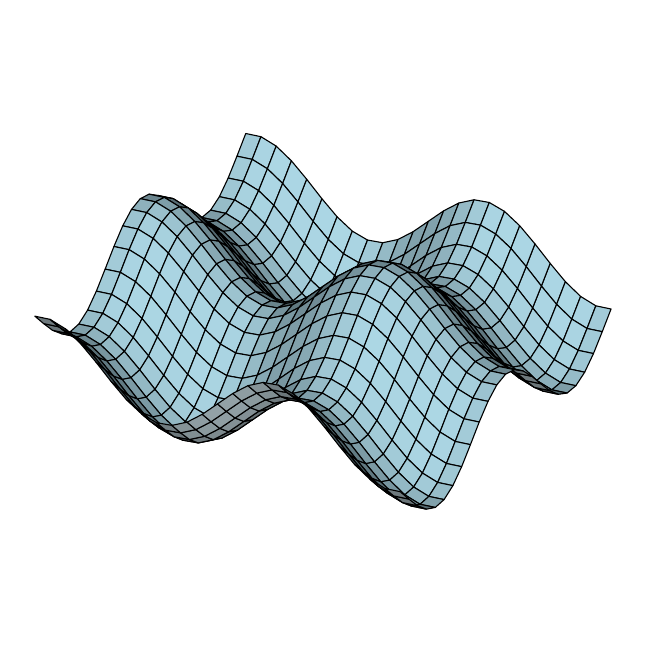
\begin{tikzpicture}%
\pgfsetxvec{\pgfxy(0.5357,0)}%
\pgfsetyvec{\pgfxy(0,0.5357)}%
\useasboundingbox (-7,-7)--(7,7);
%image  (User)
\pgfsetstrokecolor{rgb,1:red,0;green,0;blue,0}%
\pgfsetlinewidth{0.4pt}%
\pgfsetroundjoin%
\pgfpathmoveto{\pgfxy(-1.8301,4.4912)}%
\pgfpathlineto{\pgfxy(-2.0385,3.9536)}\pgfpathlineto{\pgfxy(-1.6776,3.8778)}\pgfpathlineto{\pgfxy(-1.4693,4.4154)}\pgfclosepath%
\pgfsetfillcolor{rgb,1:red,0.6392;green,0.7961;blue,0.8471}%
\pgffillstroke%
\pgfpathmoveto{\pgfxy(-2.0385,3.9536)}%
\pgfpathlineto{\pgfxy(-2.2468,3.4352)}\pgfpathlineto{\pgfxy(-1.8859,3.3594)}\pgfpathlineto{\pgfxy(-1.6776,3.8778)}\pgfclosepath%
\pgfsetfillcolor{rgb,1:red,0.6353;green,0.7961;blue,0.8471}%
\pgffillstroke%
\pgfpathmoveto{\pgfxy(-1.4693,4.4154)}%
\pgfpathlineto{\pgfxy(-1.6776,3.8778)}\pgfpathlineto{\pgfxy(-1.3168,3.6551)}\pgfpathlineto{\pgfxy(-1.1084,4.1926)}\pgfclosepath%
\pgfsetfillcolor{rgb,1:red,0.6667;green,0.8314;blue,0.8863}%
\pgffillstroke%
\pgfpathmoveto{\pgfxy(-0.0259,2.9467)}%
\pgfpathlineto{\pgfxy(-0.2342,2.4092)}\pgfpathlineto{\pgfxy(0.1266,1.9799)}\pgfpathlineto{\pgfxy(0.3349,2.5174)}\pgfclosepath%
\pgfsetfillcolor{rgb,1:red,0.6706;green,0.8392;blue,0.8941}%
\pgffillstroke%
\pgfpathmoveto{\pgfxy(-0.3868,3.4091)}%
\pgfpathlineto{\pgfxy(-0.5951,2.8716)}\pgfpathlineto{\pgfxy(-0.2342,2.4092)}\pgfpathlineto{\pgfxy(-0.0259,2.9467)}\pgfclosepath%
\pgfsetfillcolor{rgb,1:red,0.6706;green,0.8353;blue,0.8902}%
\pgffillstroke%
\pgfpathmoveto{\pgfxy(0.3349,2.5174)}%
\pgfpathlineto{\pgfxy(0.1266,1.9799)}\pgfpathlineto{\pgfxy(0.4874,1.6393)}\pgfpathlineto{\pgfxy(0.6958,2.1768)}\pgfclosepath%
\pgfsetfillcolor{rgb,1:red,0.6745;green,0.8431;blue,0.8941}%
\pgffillstroke%
\pgfpathmoveto{\pgfxy(-1.1084,4.1926)}%
\pgfpathlineto{\pgfxy(-1.3168,3.6551)}\pgfpathlineto{\pgfxy(-0.9559,3.3057)}\pgfpathlineto{\pgfxy(-0.7476,3.8432)}\pgfclosepath%
\pgfsetfillcolor{rgb,1:red,0.6745;green,0.8431;blue,0.8941}%
\pgffillstroke%
\pgfpathmoveto{\pgfxy(-0.7476,3.8432)}%
\pgfpathlineto{\pgfxy(-0.9559,3.3057)}\pgfpathlineto{\pgfxy(-0.5951,2.8716)}\pgfpathlineto{\pgfxy(-0.3868,3.4091)}\pgfclosepath%
\pgfsetfillcolor{rgb,1:red,0.6706;green,0.8392;blue,0.8941}%
\pgffillstroke%
\pgfpathmoveto{\pgfxy(-2.2468,3.4352)}%
\pgfpathlineto{\pgfxy(-2.4551,2.9936)}\pgfpathlineto{\pgfxy(-2.0943,2.9178)}\pgfpathlineto{\pgfxy(-1.8859,3.3594)}\pgfclosepath%
\pgfsetfillcolor{rgb,1:red,0.6235;green,0.7804;blue,0.8314}%
\pgffillstroke%
\pgfpathmoveto{\pgfxy(-1.6776,3.8778)}%
\pgfpathlineto{\pgfxy(-1.8859,3.3594)}\pgfpathlineto{\pgfxy(-1.5251,3.1366)}\pgfpathlineto{\pgfxy(-1.3168,3.6551)}\pgfclosepath%
\pgfsetfillcolor{rgb,1:red,0.6667;green,0.8314;blue,0.8863}%
\pgffillstroke%
\pgfpathmoveto{\pgfxy(0.6958,2.1768)}%
\pgfpathlineto{\pgfxy(0.4874,1.6393)}\pgfpathlineto{\pgfxy(0.8483,1.4278)}\pgfpathlineto{\pgfxy(1.0566,1.9653)}\pgfclosepath%
\pgfsetfillcolor{rgb,1:red,0.6667;green,0.8314;blue,0.8863}%
\pgffillstroke%
\pgfpathmoveto{\pgfxy(-0.2342,2.4092)}%
\pgfpathlineto{\pgfxy(-0.4426,1.8907)}\pgfpathlineto{\pgfxy(-0.0817,1.4614)}\pgfpathlineto{\pgfxy(0.1266,1.9799)}\pgfclosepath%
\pgfsetfillcolor{rgb,1:red,0.6706;green,0.8353;blue,0.8902}%
\pgffillstroke%
\pgfpathmoveto{\pgfxy(-0.5951,2.8716)}%
\pgfpathlineto{\pgfxy(-0.8034,2.3531)}\pgfpathlineto{\pgfxy(-0.4426,1.8907)}\pgfpathlineto{\pgfxy(-0.2342,2.4092)}\pgfclosepath%
\pgfsetfillcolor{rgb,1:red,0.6706;green,0.8353;blue,0.8902}%
\pgffillstroke%
\pgfpathmoveto{\pgfxy(0.1266,1.9799)}%
\pgfpathlineto{\pgfxy(-0.0817,1.4614)}\pgfpathlineto{\pgfxy(0.2791,1.1208)}\pgfpathlineto{\pgfxy(0.4874,1.6393)}\pgfclosepath%
\pgfsetfillcolor{rgb,1:red,0.6745;green,0.8392;blue,0.8941}%
\pgffillstroke%
\pgfpathmoveto{\pgfxy(-1.3168,3.6551)}%
\pgfpathlineto{\pgfxy(-1.5251,3.1366)}\pgfpathlineto{\pgfxy(-1.1643,2.7872)}\pgfpathlineto{\pgfxy(-0.9559,3.3057)}\pgfclosepath%
\pgfsetfillcolor{rgb,1:red,0.6745;green,0.8392;blue,0.8941}%
\pgffillstroke%
\pgfpathmoveto{\pgfxy(-0.9559,3.3057)}%
\pgfpathlineto{\pgfxy(-1.1643,2.7872)}\pgfpathlineto{\pgfxy(-0.8034,2.3531)}\pgfpathlineto{\pgfxy(-0.5951,2.8716)}\pgfclosepath%
\pgfsetfillcolor{rgb,1:red,0.6706;green,0.8353;blue,0.8902}%
\pgffillstroke%
\pgfpathmoveto{\pgfxy(-1.8859,3.3594)}%
\pgfpathlineto{\pgfxy(-2.0943,2.9178)}\pgfpathlineto{\pgfxy(-1.7334,2.6951)}\pgfpathlineto{\pgfxy(-1.5251,3.1366)}\pgfclosepath%
\pgfsetfillcolor{rgb,1:red,0.6588;green,0.8235;blue,0.8745}%
\pgffillstroke%
\pgfpathmoveto{\pgfxy(0.4874,1.6393)}%
\pgfpathlineto{\pgfxy(0.2791,1.1208)}\pgfpathlineto{\pgfxy(0.64,0.9093)}\pgfpathlineto{\pgfxy(0.8483,1.4278)}\pgfclosepath%
\pgfsetfillcolor{rgb,1:red,0.6627;green,0.8314;blue,0.8824}%
\pgffillstroke%
\pgfpathmoveto{\pgfxy(-2.4551,2.9936)}%
\pgfpathlineto{\pgfxy(-2.6635,2.6737)}\pgfpathlineto{\pgfxy(-2.3026,2.5979)}\pgfpathlineto{\pgfxy(-2.0943,2.9178)}\pgfclosepath%
\pgfsetfillcolor{rgb,1:red,0.5882;green,0.7373;blue,0.7843}%
\pgffillstroke%
\pgfpathmoveto{\pgfxy(-0.4426,1.8907)}%
\pgfpathlineto{\pgfxy(-0.6509,1.4492)}\pgfpathlineto{\pgfxy(-0.2901,1.0199)}\pgfpathlineto{\pgfxy(-0.0817,1.4614)}\pgfclosepath%
\pgfsetfillcolor{rgb,1:red,0.6627;green,0.8275;blue,0.8784}%
\pgffillstroke%
\pgfpathmoveto{\pgfxy(1.0566,1.9653)}%
\pgfpathlineto{\pgfxy(0.8483,1.4278)}\pgfpathlineto{\pgfxy(1.2091,1.3638)}\pgfpathlineto{\pgfxy(1.4175,1.9014)}\pgfclosepath%
\pgfsetfillcolor{rgb,1:red,0.6353;green,0.7922;blue,0.8431}%
\pgffillstroke%
\pgfpathmoveto{\pgfxy(-0.8034,2.3531)}%
\pgfpathlineto{\pgfxy(-1.0118,1.9115)}\pgfpathlineto{\pgfxy(-0.6509,1.4492)}\pgfpathlineto{\pgfxy(-0.4426,1.8907)}\pgfclosepath%
\pgfsetfillcolor{rgb,1:red,0.6588;green,0.8235;blue,0.8745}%
\pgffillstroke%
\pgfpathmoveto{\pgfxy(-0.0817,1.4614)}%
\pgfpathlineto{\pgfxy(-0.2901,1.0199)}\pgfpathlineto{\pgfxy(0.0708,0.6793)}\pgfpathlineto{\pgfxy(0.2791,1.1208)}\pgfclosepath%
\pgfsetfillcolor{rgb,1:red,0.6627;green,0.8314;blue,0.8824}%
\pgffillstroke%
\pgfpathmoveto{\pgfxy(-1.5251,3.1366)}%
\pgfpathlineto{\pgfxy(-1.7334,2.6951)}\pgfpathlineto{\pgfxy(-1.3726,2.3457)}\pgfpathlineto{\pgfxy(-1.1643,2.7872)}\pgfclosepath%
\pgfsetfillcolor{rgb,1:red,0.6627;green,0.8314;blue,0.8824}%
\pgffillstroke%
\pgfpathmoveto{\pgfxy(-1.1643,2.7872)}%
\pgfpathlineto{\pgfxy(-1.3726,2.3457)}\pgfpathlineto{\pgfxy(-1.0118,1.9115)}\pgfpathlineto{\pgfxy(-0.8034,2.3531)}\pgfclosepath%
\pgfsetfillcolor{rgb,1:red,0.6627;green,0.8235;blue,0.8784}%
\pgffillstroke%
\pgfpathmoveto{\pgfxy(0.2791,1.1208)}%
\pgfpathlineto{\pgfxy(0.0708,0.6793)}\pgfpathlineto{\pgfxy(0.4316,0.4678)}\pgfpathlineto{\pgfxy(0.64,0.9093)}\pgfclosepath%
\pgfsetfillcolor{rgb,1:red,0.6588;green,0.8196;blue,0.8745}%
\pgffillstroke%
\pgfpathmoveto{\pgfxy(0.8483,1.4278)}%
\pgfpathlineto{\pgfxy(0.64,0.9093)}\pgfpathlineto{\pgfxy(1.0008,0.8454)}\pgfpathlineto{\pgfxy(1.2091,1.3638)}\pgfclosepath%
\pgfsetfillcolor{rgb,1:red,0.6314;green,0.7882;blue,0.8392}%
\pgffillstroke%
\pgfpathmoveto{\pgfxy(-2.0943,2.9178)}%
\pgfpathlineto{\pgfxy(-2.3026,2.5979)}\pgfpathlineto{\pgfxy(-1.9418,2.3751)}\pgfpathlineto{\pgfxy(-1.7334,2.6951)}\pgfclosepath%
\pgfsetfillcolor{rgb,1:red,0.6314;green,0.7882;blue,0.8392}%
\pgffillstroke%
\pgfpathmoveto{\pgfxy(-0.6509,1.4492)}%
\pgfpathlineto{\pgfxy(-0.8592,1.1292)}\pgfpathlineto{\pgfxy(-0.4984,0.6999)}\pgfpathlineto{\pgfxy(-0.2901,1.0199)}\pgfclosepath%
\pgfsetfillcolor{rgb,1:red,0.6353;green,0.7922;blue,0.8431}%
\pgffillstroke%
\pgfpathmoveto{\pgfxy(-1.0118,1.9115)}%
\pgfpathlineto{\pgfxy(-1.2201,1.5916)}\pgfpathlineto{\pgfxy(-0.8592,1.1292)}\pgfpathlineto{\pgfxy(-0.6509,1.4492)}\pgfclosepath%
\pgfsetfillcolor{rgb,1:red,0.6314;green,0.7882;blue,0.8392}%
\pgffillstroke%
\pgfpathmoveto{\pgfxy(-0.2901,1.0199)}%
\pgfpathlineto{\pgfxy(-0.4984,0.6999)}\pgfpathlineto{\pgfxy(-0.1376,0.3593)}\pgfpathlineto{\pgfxy(0.0708,0.6793)}\pgfclosepath%
\pgfsetfillcolor{rgb,1:red,0.6353;green,0.7961;blue,0.8471}%
\pgffillstroke%
\pgfpathmoveto{\pgfxy(-1.7334,2.6951)}%
\pgfpathlineto{\pgfxy(-1.9418,2.3751)}\pgfpathlineto{\pgfxy(-1.5809,2.0257)}\pgfpathlineto{\pgfxy(-1.3726,2.3457)}\pgfclosepath%
\pgfsetfillcolor{rgb,1:red,0.6353;green,0.7961;blue,0.8471}%
\pgffillstroke%
\pgfpathmoveto{\pgfxy(-1.3726,2.3457)}%
\pgfpathlineto{\pgfxy(-1.5809,2.0257)}\pgfpathlineto{\pgfxy(-1.2201,1.5916)}\pgfpathlineto{\pgfxy(-1.0118,1.9115)}\pgfclosepath%
\pgfsetfillcolor{rgb,1:red,0.6314;green,0.7922;blue,0.8431}%
\pgffillstroke%
\pgfpathmoveto{\pgfxy(1.4175,1.9014)}%
\pgfpathlineto{\pgfxy(1.2091,1.3638)}\pgfpathlineto{\pgfxy(1.57,1.4405)}\pgfpathlineto{\pgfxy(1.7783,1.978)}\pgfclosepath%
\pgfsetfillcolor{rgb,1:red,0.5843;green,0.7294;blue,0.7765}%
\pgffillstroke%
\pgfpathmoveto{\pgfxy(0.64,0.9093)}%
\pgfpathlineto{\pgfxy(0.4316,0.4678)}\pgfpathlineto{\pgfxy(0.7925,0.4038)}\pgfpathlineto{\pgfxy(1.0008,0.8454)}\pgfclosepath%
\pgfsetfillcolor{rgb,1:red,0.6196;green,0.7765;blue,0.8275}%
\pgffillstroke%
\pgfpathmoveto{\pgfxy(-2.6635,2.6737)}%
\pgfpathlineto{\pgfxy(-2.8718,2.4992)}\pgfpathlineto{\pgfxy(-2.5109,2.4234)}\pgfpathlineto{\pgfxy(-2.3026,2.5979)}\pgfclosepath%
\pgfsetfillcolor{rgb,1:red,0.4941;green,0.6157;blue,0.6549}%
\pgffillstroke%
\pgfpathmoveto{\pgfxy(0.0708,0.6793)}%
\pgfpathlineto{\pgfxy(-0.1376,0.3593)}\pgfpathlineto{\pgfxy(0.2233,0.1478)}\pgfpathlineto{\pgfxy(0.4316,0.4678)}\pgfclosepath%
\pgfsetfillcolor{rgb,1:red,0.6275;green,0.7843;blue,0.8353}%
\pgffillstroke%
\pgfpathmoveto{\pgfxy(1.2091,1.3638)}%
\pgfpathlineto{\pgfxy(1.0008,0.8454)}\pgfpathlineto{\pgfxy(1.3616,0.922)}\pgfpathlineto{\pgfxy(1.57,1.4405)}\pgfclosepath%
\pgfsetfillcolor{rgb,1:red,0.5804;green,0.7255;blue,0.7725}%
\pgffillstroke%
\pgfpathmoveto{\pgfxy(-2.3026,2.5979)}%
\pgfpathlineto{\pgfxy(-2.5109,2.4234)}\pgfpathlineto{\pgfxy(-2.1501,2.2006)}\pgfpathlineto{\pgfxy(-1.9418,2.3751)}\pgfclosepath%
\pgfsetfillcolor{rgb,1:red,0.5529;green,0.6902;blue,0.7333}%
\pgffillstroke%
\pgfpathmoveto{\pgfxy(0.4316,0.4678)}%
\pgfpathlineto{\pgfxy(0.2233,0.1478)}\pgfpathlineto{\pgfxy(0.5841,0.0839)}\pgfpathlineto{\pgfxy(0.7925,0.4038)}\pgfclosepath%
\pgfsetfillcolor{rgb,1:red,0.5843;green,0.7294;blue,0.7765}%
\pgffillstroke%
\pgfpathmoveto{\pgfxy(-0.8592,1.1292)}%
\pgfpathlineto{\pgfxy(-1.0676,0.9548)}\pgfpathlineto{\pgfxy(-0.7067,0.5255)}\pgfpathlineto{\pgfxy(-0.4984,0.6999)}\pgfclosepath%
\pgfsetfillcolor{rgb,1:red,0.5725;green,0.7137;blue,0.7608}%
\pgffillstroke%
\pgfpathmoveto{\pgfxy(-1.2201,1.5916)}%
\pgfpathlineto{\pgfxy(-1.4284,1.4171)}\pgfpathlineto{\pgfxy(-1.0676,0.9548)}\pgfpathlineto{\pgfxy(-0.8592,1.1292)}\pgfclosepath%
\pgfsetfillcolor{rgb,1:red,0.5725;green,0.7137;blue,0.7608}%
\pgffillstroke%
\pgfpathmoveto{\pgfxy(-0.4984,0.6999)}%
\pgfpathlineto{\pgfxy(-0.7067,0.5255)}\pgfpathlineto{\pgfxy(-0.3459,0.1848)}\pgfpathlineto{\pgfxy(-0.1376,0.3593)}\pgfclosepath%
\pgfsetfillcolor{rgb,1:red,0.5686;green,0.7098;blue,0.7569}%
\pgffillstroke%
\pgfpathmoveto{\pgfxy(-1.9418,2.3751)}%
\pgfpathlineto{\pgfxy(-2.1501,2.2006)}\pgfpathlineto{\pgfxy(-1.7893,1.8512)}\pgfpathlineto{\pgfxy(-1.5809,2.0257)}\pgfclosepath%
\pgfsetfillcolor{rgb,1:red,0.5686;green,0.7098;blue,0.7569}%
\pgffillstroke%
\pgfpathmoveto{\pgfxy(1.0008,0.8454)}%
\pgfpathlineto{\pgfxy(0.7925,0.4038)}\pgfpathlineto{\pgfxy(1.1533,0.4805)}\pgfpathlineto{\pgfxy(1.3616,0.922)}\pgfclosepath%
\pgfsetfillcolor{rgb,1:red,0.5608;green,0.698;blue,0.7451}%
\pgffillstroke%
\pgfpathmoveto{\pgfxy(-1.5809,2.0257)}%
\pgfpathlineto{\pgfxy(-1.7893,1.8512)}\pgfpathlineto{\pgfxy(-1.4284,1.4171)}\pgfpathlineto{\pgfxy(-1.2201,1.5916)}\pgfclosepath%
\pgfsetfillcolor{rgb,1:red,0.5725;green,0.7137;blue,0.7608}%
\pgffillstroke%
\pgfpathmoveto{\pgfxy(1.7783,1.978)}%
\pgfpathlineto{\pgfxy(1.57,1.4405)}\pgfpathlineto{\pgfxy(1.9308,1.6269)}\pgfpathlineto{\pgfxy(2.1392,2.1644)}\pgfclosepath%
\pgfsetfillcolor{rgb,1:red,0.5333;green,0.6667;blue,0.7098}%
\pgffillstroke%
\pgfpathmoveto{\pgfxy(-0.1376,0.3593)}%
\pgfpathlineto{\pgfxy(-0.3459,0.1848)}\pgfpathlineto{\pgfxy(0.015,-0.0266)}\pgfpathlineto{\pgfxy(0.2233,0.1478)}\pgfclosepath%
\pgfsetfillcolor{rgb,1:red,0.549;green,0.6863;blue,0.7294}%
\pgffillstroke%
\pgfpathmoveto{\pgfxy(-2.8718,2.4992)}%
\pgfpathlineto{\pgfxy(-3.0801,2.4692)}\pgfpathlineto{\pgfxy(-2.7193,2.3934)}\pgfpathlineto{\pgfxy(-2.5109,2.4234)}\pgfclosepath%
\pgfsetfillcolor{rgb,1:red,0.3098;green,0.3882;blue,0.4118}%
\pgffillstroke%
\pgfpathmoveto{\pgfxy(1.57,1.4405)}%
\pgfpathlineto{\pgfxy(1.3616,0.922)}\pgfpathlineto{\pgfxy(1.7225,1.1084)}\pgfpathlineto{\pgfxy(1.9308,1.6269)}\pgfclosepath%
\pgfsetfillcolor{rgb,1:red,0.5294;green,0.6588;blue,0.702}%
\pgffillstroke%
\pgfpathmoveto{\pgfxy(0.7925,0.4038)}%
\pgfpathlineto{\pgfxy(0.5841,0.0839)}\pgfpathlineto{\pgfxy(0.945,0.1605)}\pgfpathlineto{\pgfxy(1.1533,0.4805)}\pgfclosepath%
\pgfsetfillcolor{rgb,1:red,0.5059;green,0.6353;blue,0.6745}%
\pgffillstroke%
\pgfpathmoveto{\pgfxy(0.2233,0.1478)}%
\pgfpathlineto{\pgfxy(0.015,-0.0266)}\pgfpathlineto{\pgfxy(0.3758,-0.0906)}\pgfpathlineto{\pgfxy(0.5841,0.0839)}\pgfclosepath%
\pgfsetfillcolor{rgb,1:red,0.4863;green,0.6078;blue,0.6471}%
\pgffillstroke%
\pgfpathmoveto{\pgfxy(-2.5109,2.4234)}%
\pgfpathlineto{\pgfxy(-2.7193,2.3934)}\pgfpathlineto{\pgfxy(-2.3584,2.1706)}\pgfpathlineto{\pgfxy(-2.1501,2.2006)}\pgfclosepath%
\pgfsetfillcolor{rgb,1:red,0.4157;green,0.5176;blue,0.549}%
\pgffillstroke%
\pgfpathmoveto{\pgfxy(1.3616,0.922)}%
\pgfpathlineto{\pgfxy(1.1533,0.4805)}\pgfpathlineto{\pgfxy(1.5142,0.6668)}\pgfpathlineto{\pgfxy(1.7225,1.1084)}\pgfclosepath%
\pgfsetfillcolor{rgb,1:red,0.502;green,0.6275;blue,0.6667}%
\pgffillstroke%
\pgfpathmoveto{\pgfxy(-1.0676,0.9548)}%
\pgfpathlineto{\pgfxy(-1.2759,0.9247)}\pgfpathlineto{\pgfxy(-0.9151,0.4954)}\pgfpathlineto{\pgfxy(-0.7067,0.5255)}\pgfclosepath%
\pgfsetfillcolor{rgb,1:red,0.4745;green,0.5922;blue,0.6314}%
\pgffillstroke%
\pgfpathmoveto{\pgfxy(-1.4284,1.4171)}%
\pgfpathlineto{\pgfxy(-1.6368,1.3871)}\pgfpathlineto{\pgfxy(-1.2759,0.9247)}\pgfpathlineto{\pgfxy(-1.0676,0.9548)}\pgfclosepath%
\pgfsetfillcolor{rgb,1:red,0.4784;green,0.6;blue,0.6392}%
\pgffillstroke%
\pgfpathmoveto{\pgfxy(-0.7067,0.5255)}%
\pgfpathlineto{\pgfxy(-0.9151,0.4954)}\pgfpathlineto{\pgfxy(-0.5542,0.1548)}\pgfpathlineto{\pgfxy(-0.3459,0.1848)}\pgfclosepath%
\pgfsetfillcolor{rgb,1:red,0.4549;green,0.5686;blue,0.6078}%
\pgffillstroke%
\pgfpathmoveto{\pgfxy(-2.1501,2.2006)}%
\pgfpathlineto{\pgfxy(-2.3584,2.1706)}\pgfpathlineto{\pgfxy(-1.9976,1.8212)}\pgfpathlineto{\pgfxy(-1.7893,1.8512)}\pgfclosepath%
\pgfsetfillcolor{rgb,1:red,0.4588;green,0.5725;blue,0.6118}%
\pgffillstroke%
\pgfpathmoveto{\pgfxy(-1.7893,1.8512)}%
\pgfpathlineto{\pgfxy(-1.9976,1.8212)}\pgfpathlineto{\pgfxy(-1.6368,1.3871)}\pgfpathlineto{\pgfxy(-1.4284,1.4171)}\pgfclosepath%
\pgfsetfillcolor{rgb,1:red,0.4745;green,0.5922;blue,0.6314}%
\pgffillstroke%
\pgfpathmoveto{\pgfxy(-0.3459,0.1848)}%
\pgfpathlineto{\pgfxy(-0.5542,0.1548)}\pgfpathlineto{\pgfxy(-0.1934,-0.0567)}\pgfpathlineto{\pgfxy(0.015,-0.0266)}\pgfclosepath%
\pgfsetfillcolor{rgb,1:red,0.4078;green,0.5098;blue,0.5451}%
\pgffillstroke%
\pgfpathmoveto{\pgfxy(2.1392,2.1644)}%
\pgfpathlineto{\pgfxy(1.9308,1.6269)}\pgfpathlineto{\pgfxy(2.2917,1.8732)}\pgfpathlineto{\pgfxy(2.5,2.4107)}\pgfclosepath%
\pgfsetfillcolor{rgb,1:red,0.5059;green,0.6314;blue,0.6745}%
\pgffillstroke%
\pgfpathmoveto{\pgfxy(0.5841,0.0839)}%
\pgfpathlineto{\pgfxy(0.3758,-0.0906)}\pgfpathlineto{\pgfxy(0.7366,-0.0139)}\pgfpathlineto{\pgfxy(0.945,0.1605)}\pgfclosepath%
\pgfsetfillcolor{rgb,1:red,0.3843;green,0.4784;blue,0.5098}%
\pgffillstroke%
\pgfpathmoveto{\pgfxy(1.1533,0.4805)}%
\pgfpathlineto{\pgfxy(0.945,0.1605)}\pgfpathlineto{\pgfxy(1.3058,0.3469)}\pgfpathlineto{\pgfxy(1.5142,0.6668)}\pgfclosepath%
\pgfsetfillcolor{rgb,1:red,0.4353;green,0.5412;blue,0.5765}%
\pgffillstroke%
\pgfpathmoveto{\pgfxy(1.9308,1.6269)}%
\pgfpathlineto{\pgfxy(1.7225,1.1084)}\pgfpathlineto{\pgfxy(2.0833,1.3547)}\pgfpathlineto{\pgfxy(2.2917,1.8732)}\pgfclosepath%
\pgfsetfillcolor{rgb,1:red,0.498;green,0.6235;blue,0.6627}%
\pgffillstroke%
\pgfpathmoveto{\pgfxy(-3.0801,2.4692)}%
\pgfpathlineto{\pgfxy(-3.2885,2.5579)}\pgfpathlineto{\pgfxy(-2.9276,2.4821)}\pgfpathlineto{\pgfxy(-2.7193,2.3934)}\pgfclosepath%
\pgfsetfillcolor{rgb,1:red,0.2941;green,0.3255;blue,0.3373}%
\pgffillstroke%
\pgfpathmoveto{\pgfxy(0.015,-0.0266)}%
\pgfpathlineto{\pgfxy(-0.1934,-0.0567)}\pgfpathlineto{\pgfxy(0.1675,-0.1206)}\pgfpathlineto{\pgfxy(0.3758,-0.0906)}\pgfclosepath%
\pgfsetfillcolor{rgb,1:red,0.298;green,0.3725;blue,0.3961}%
\pgffillstroke%
\pgfpathmoveto{\pgfxy(1.7225,1.1084)}%
\pgfpathlineto{\pgfxy(1.5142,0.6668)}\pgfpathlineto{\pgfxy(1.875,0.9132)}\pgfpathlineto{\pgfxy(2.0833,1.3547)}\pgfclosepath%
\pgfsetfillcolor{rgb,1:red,0.4667;green,0.5843;blue,0.6235}%
\pgffillstroke%
\pgfpathmoveto{\pgfxy(-2.7193,2.3934)}%
\pgfpathlineto{\pgfxy(-2.9276,2.4821)}\pgfpathlineto{\pgfxy(-2.5668,2.2593)}\pgfpathlineto{\pgfxy(-2.3584,2.1706)}\pgfclosepath%
\pgfsetfillcolor{rgb,1:red,0.2275;green,0.2824;blue,0.302}%
\pgffillstroke%
\pgfpathmoveto{\pgfxy(-1.2759,0.9247)}%
\pgfpathlineto{\pgfxy(-1.4842,1.0134)}\pgfpathlineto{\pgfxy(-1.1234,0.5841)}\pgfpathlineto{\pgfxy(-0.9151,0.4954)}\pgfclosepath%
\pgfsetfillcolor{rgb,1:red,0.3686;green,0.4588;blue,0.4863}%
\pgffillstroke%
\pgfpathmoveto{\pgfxy(-1.6368,1.3871)}%
\pgfpathlineto{\pgfxy(-1.8451,1.4758)}\pgfpathlineto{\pgfxy(-1.4842,1.0134)}\pgfpathlineto{\pgfxy(-1.2759,0.9247)}\pgfclosepath%
\pgfsetfillcolor{rgb,1:red,0.3765;green,0.4706;blue,0.502}%
\pgffillstroke%
\pgfpathmoveto{\pgfxy(-0.9151,0.4954)}%
\pgfpathlineto{\pgfxy(-1.1234,0.5841)}\pgfpathlineto{\pgfxy(-0.7626,0.2435)}\pgfpathlineto{\pgfxy(-0.5542,0.1548)}\pgfclosepath%
\pgfsetfillcolor{rgb,1:red,0.3255;green,0.4078;blue,0.4314}%
\pgffillstroke%
\pgfpathmoveto{\pgfxy(-2.3584,2.1706)}%
\pgfpathlineto{\pgfxy(-2.5668,2.2593)}\pgfpathlineto{\pgfxy(-2.2059,1.9099)}\pgfpathlineto{\pgfxy(-1.9976,1.8212)}\pgfclosepath%
\pgfsetfillcolor{rgb,1:red,0.3294;green,0.4118;blue,0.4392}%
\pgffillstroke%
\pgfpathmoveto{\pgfxy(0.945,0.1605)}%
\pgfpathlineto{\pgfxy(0.7366,-0.0139)}\pgfpathlineto{\pgfxy(1.0975,0.1724)}\pgfpathlineto{\pgfxy(1.3058,0.3469)}\pgfclosepath%
\pgfsetfillcolor{rgb,1:red,0.2784;green,0.349;blue,0.3725}%
\pgffillstroke%
\pgfpathmoveto{\pgfxy(-1.9976,1.8212)}%
\pgfpathlineto{\pgfxy(-2.2059,1.9099)}\pgfpathlineto{\pgfxy(-1.8451,1.4758)}\pgfpathlineto{\pgfxy(-1.6368,1.3871)}\pgfclosepath%
\pgfsetfillcolor{rgb,1:red,0.3686;green,0.4588;blue,0.4902}%
\pgffillstroke%
\pgfpathmoveto{\pgfxy(2.5,2.4107)}%
\pgfpathlineto{\pgfxy(2.2917,1.8732)}\pgfpathlineto{\pgfxy(2.6525,2.1195)}\pgfpathlineto{\pgfxy(2.8608,2.657)}\pgfclosepath%
\pgfsetfillcolor{rgb,1:red,0.5059;green,0.6314;blue,0.6745}%
\pgffillstroke%
\pgfpathmoveto{\pgfxy(0.3758,-0.0906)}%
\pgfpathlineto{\pgfxy(0.1675,-0.1206)}\pgfpathlineto{\pgfxy(0.5283,-0.044)}\pgfpathlineto{\pgfxy(0.7366,-0.0139)}\pgfclosepath%
\pgfsetfillcolor{rgb,1:red,0.1922;green,0.2118;blue,0.2157}%
\pgffillstroke%
\pgfpathmoveto{\pgfxy(-0.5542,0.1548)}%
\pgfpathlineto{\pgfxy(-0.7626,0.2435)}\pgfpathlineto{\pgfxy(-0.4017,0.032)}\pgfpathlineto{\pgfxy(-0.1934,-0.0567)}\pgfclosepath%
\pgfsetfillcolor{rgb,1:red,0.2118;green,0.2627;blue,0.2824}%
\pgffillstroke%
\pgfpathmoveto{\pgfxy(1.5142,0.6668)}%
\pgfpathlineto{\pgfxy(1.3058,0.3469)}\pgfpathlineto{\pgfxy(1.6667,0.5932)}\pgfpathlineto{\pgfxy(1.875,0.9132)}\pgfclosepath%
\pgfsetfillcolor{rgb,1:red,0.3922;green,0.4902;blue,0.5216}%
\pgffillstroke%
\pgfpathmoveto{\pgfxy(2.2917,1.8732)}%
\pgfpathlineto{\pgfxy(2.0833,1.3547)}\pgfpathlineto{\pgfxy(2.4442,1.601)}\pgfpathlineto{\pgfxy(2.6525,2.1195)}\pgfclosepath%
\pgfsetfillcolor{rgb,1:red,0.498;green,0.6235;blue,0.6627}%
\pgffillstroke%
\pgfpathmoveto{\pgfxy(-0.1934,-0.0567)}%
\pgfpathlineto{\pgfxy(-0.4017,0.032)}\pgfpathlineto{\pgfxy(-0.0409,-0.0319)}\pgfpathlineto{\pgfxy(0.1675,-0.1206)}\pgfclosepath%
\pgfsetfillcolor{rgb,1:red,0.3137;green,0.3451;blue,0.3569}%
\pgffillstroke%
\pgfpathmoveto{\pgfxy(-3.2885,2.5579)}%
\pgfpathlineto{\pgfxy(-3.4968,2.7192)}\pgfpathlineto{\pgfxy(-3.1359,2.6434)}\pgfpathlineto{\pgfxy(-2.9276,2.4821)}\pgfclosepath%
\pgfsetfillcolor{rgb,1:red,0.4196;green,0.4627;blue,0.4745}%
\pgffillstroke%
\pgfpathmoveto{\pgfxy(2.0833,1.3547)}%
\pgfpathlineto{\pgfxy(1.875,0.9132)}\pgfpathlineto{\pgfxy(2.2358,1.1595)}\pgfpathlineto{\pgfxy(2.4442,1.601)}\pgfclosepath%
\pgfsetfillcolor{rgb,1:red,0.4667;green,0.5843;blue,0.6235}%
\pgffillstroke%
\pgfpathmoveto{\pgfxy(0.7366,-0.0139)}%
\pgfpathlineto{\pgfxy(0.5283,-0.044)}\pgfpathlineto{\pgfxy(0.8892,0.1424)}\pgfpathlineto{\pgfxy(1.0975,0.1724)}\pgfclosepath%
\pgfsetfillcolor{rgb,1:red,0.3569;green,0.3922;blue,0.4039}%
\pgffillstroke%
\pgfpathmoveto{\pgfxy(1.3058,0.3469)}%
\pgfpathlineto{\pgfxy(1.0975,0.1724)}\pgfpathlineto{\pgfxy(1.4583,0.4187)}\pgfpathlineto{\pgfxy(1.6667,0.5932)}\pgfclosepath%
\pgfsetfillcolor{rgb,1:red,0.2;green,0.251;blue,0.2667}%
\pgffillstroke%
\pgfpathmoveto{\pgfxy(2.8608,2.657)}%
\pgfpathlineto{\pgfxy(2.6525,2.1195)}\pgfpathlineto{\pgfxy(3.0134,2.3059)}\pgfpathlineto{\pgfxy(3.2217,2.8434)}\pgfclosepath%
\pgfsetfillcolor{rgb,1:red,0.5333;green,0.6667;blue,0.7098}%
\pgffillstroke%
\pgfpathmoveto{\pgfxy(-2.9276,2.4821)}%
\pgfpathlineto{\pgfxy(-3.1359,2.6434)}\pgfpathlineto{\pgfxy(-2.7751,2.4207)}\pgfpathlineto{\pgfxy(-2.5668,2.2593)}\pgfclosepath%
\pgfsetfillcolor{rgb,1:red,0.2471;green,0.2745;blue,0.2824}%
\pgffillstroke%
\pgfpathmoveto{\pgfxy(-1.4842,1.0134)}%
\pgfpathlineto{\pgfxy(-1.6926,1.1748)}\pgfpathlineto{\pgfxy(-1.3317,0.7455)}\pgfpathlineto{\pgfxy(-1.1234,0.5841)}\pgfclosepath%
\pgfsetfillcolor{rgb,1:red,0.2784;green,0.349;blue,0.3725}%
\pgffillstroke%
\pgfpathmoveto{\pgfxy(1.875,0.9132)}%
\pgfpathlineto{\pgfxy(1.6667,0.5932)}\pgfpathlineto{\pgfxy(2.0275,0.8395)}\pgfpathlineto{\pgfxy(2.2358,1.1595)}\pgfclosepath%
\pgfsetfillcolor{rgb,1:red,0.3922;green,0.4902;blue,0.5216}%
\pgffillstroke%
\pgfpathmoveto{\pgfxy(0.1675,-0.1206)}%
\pgfpathlineto{\pgfxy(-0.0409,-0.0319)}\pgfpathlineto{\pgfxy(0.32,0.0447)}\pgfpathlineto{\pgfxy(0.5283,-0.044)}\pgfclosepath%
\pgfsetfillcolor{rgb,1:red,0.4431;green,0.4902;blue,0.5059}%
\pgffillstroke%
\pgfpathmoveto{\pgfxy(-1.8451,1.4758)}%
\pgfpathlineto{\pgfxy(-2.0534,1.6372)}\pgfpathlineto{\pgfxy(-1.6926,1.1748)}\pgfpathlineto{\pgfxy(-1.4842,1.0134)}\pgfclosepath%
\pgfsetfillcolor{rgb,1:red,0.298;green,0.3725;blue,0.3961}%
\pgffillstroke%
\pgfpathmoveto{\pgfxy(-1.1234,0.5841)}%
\pgfpathlineto{\pgfxy(-1.3317,0.7455)}\pgfpathlineto{\pgfxy(-0.9709,0.4049)}\pgfpathlineto{\pgfxy(-0.7626,0.2435)}\pgfclosepath%
\pgfsetfillcolor{rgb,1:red,0.2;green,0.251;blue,0.2667}%
\pgffillstroke%
\pgfpathmoveto{\pgfxy(-2.5668,2.2593)}%
\pgfpathlineto{\pgfxy(-2.7751,2.4207)}\pgfpathlineto{\pgfxy(-2.4143,2.0713)}\pgfpathlineto{\pgfxy(-2.2059,1.9099)}\pgfclosepath%
\pgfsetfillcolor{rgb,1:red,0.2118;green,0.2667;blue,0.2824}%
\pgffillstroke%
\pgfpathmoveto{\pgfxy(-2.2059,1.9099)}%
\pgfpathlineto{\pgfxy(-2.4143,2.0713)}\pgfpathlineto{\pgfxy(-2.0534,1.6372)}\pgfpathlineto{\pgfxy(-1.8451,1.4758)}\pgfclosepath%
\pgfsetfillcolor{rgb,1:red,0.2824;green,0.3529;blue,0.3765}%
\pgffillstroke%
\pgfpathmoveto{\pgfxy(2.6525,2.1195)}%
\pgfpathlineto{\pgfxy(2.4442,1.601)}\pgfpathlineto{\pgfxy(2.805,1.7874)}\pgfpathlineto{\pgfxy(3.0134,2.3059)}\pgfclosepath%
\pgfsetfillcolor{rgb,1:red,0.5294;green,0.6588;blue,0.702}%
\pgffillstroke%
\pgfpathmoveto{\pgfxy(-0.7626,0.2435)}%
\pgfpathlineto{\pgfxy(-0.9709,0.4049)}\pgfpathlineto{\pgfxy(-0.61,0.1934)}\pgfpathlineto{\pgfxy(-0.4017,0.032)}\pgfclosepath%
\pgfsetfillcolor{rgb,1:red,0.2667;green,0.2941;blue,0.302}%
\pgffillstroke%
\pgfpathmoveto{\pgfxy(2.4442,1.601)}%
\pgfpathlineto{\pgfxy(2.2358,1.1595)}\pgfpathlineto{\pgfxy(2.5967,1.3459)}\pgfpathlineto{\pgfxy(2.805,1.7874)}\pgfclosepath%
\pgfsetfillcolor{rgb,1:red,0.502;green,0.6275;blue,0.6667}%
\pgffillstroke%
\pgfpathmoveto{\pgfxy(3.2217,2.8434)}%
\pgfpathlineto{\pgfxy(3.0134,2.3059)}\pgfpathlineto{\pgfxy(3.3742,2.3825)}\pgfpathlineto{\pgfxy(3.5825,2.9201)}\pgfclosepath%
\pgfsetfillcolor{rgb,1:red,0.5843;green,0.7294;blue,0.7765}%
\pgffillstroke%
\pgfpathmoveto{\pgfxy(-0.4017,0.032)}%
\pgfpathlineto{\pgfxy(-0.61,0.1934)}\pgfpathlineto{\pgfxy(-0.2492,0.1294)}\pgfpathlineto{\pgfxy(-0.0409,-0.0319)}\pgfclosepath%
\pgfsetfillcolor{rgb,1:red,0.4275;green,0.4706;blue,0.4863}%
\pgffillstroke%
\pgfpathmoveto{\pgfxy(1.0975,0.1724)}%
\pgfpathlineto{\pgfxy(0.8892,0.1424)}\pgfpathlineto{\pgfxy(1.25,0.3887)}\pgfpathlineto{\pgfxy(1.4583,0.4187)}\pgfclosepath%
\pgfsetfillcolor{rgb,1:red,0.4;green,0.4431;blue,0.4549}%
\pgffillstroke%
\pgfpathmoveto{\pgfxy(1.6667,0.5932)}%
\pgfpathlineto{\pgfxy(1.4583,0.4187)}\pgfpathlineto{\pgfxy(1.8192,0.6651)}\pgfpathlineto{\pgfxy(2.0275,0.8395)}\pgfclosepath%
\pgfsetfillcolor{rgb,1:red,0.2;green,0.251;blue,0.2667}%
\pgffillstroke%
\pgfpathmoveto{\pgfxy(-3.4968,2.7192)}%
\pgfpathlineto{\pgfxy(-3.7051,2.8948)}\pgfpathlineto{\pgfxy(-3.3443,2.819)}\pgfpathlineto{\pgfxy(-3.1359,2.6434)}\pgfclosepath%
\pgfsetfillcolor{rgb,1:red,0.4353;green,0.4784;blue,0.4941}%
\pgffillstroke%
\pgfpathmoveto{\pgfxy(0.5283,-0.044)}%
\pgfpathlineto{\pgfxy(0.32,0.0447)}\pgfpathlineto{\pgfxy(0.6808,0.2311)}\pgfpathlineto{\pgfxy(0.8892,0.1424)}\pgfclosepath%
\pgfsetfillcolor{rgb,1:red,0.498;green,0.549;blue,0.5647}%
\pgffillstroke%
\pgfpathmoveto{\pgfxy(3.0134,2.3059)}%
\pgfpathlineto{\pgfxy(2.805,1.7874)}\pgfpathlineto{\pgfxy(3.1659,1.8641)}\pgfpathlineto{\pgfxy(3.3742,2.3825)}\pgfclosepath%
\pgfsetfillcolor{rgb,1:red,0.5804;green,0.7255;blue,0.7725}%
\pgffillstroke%
\pgfpathmoveto{\pgfxy(2.2358,1.1595)}%
\pgfpathlineto{\pgfxy(2.0275,0.8395)}\pgfpathlineto{\pgfxy(2.3884,1.0259)}\pgfpathlineto{\pgfxy(2.5967,1.3459)}\pgfclosepath%
\pgfsetfillcolor{rgb,1:red,0.4353;green,0.5412;blue,0.5765}%
\pgffillstroke%
\pgfpathmoveto{\pgfxy(-3.1359,2.6434)}%
\pgfpathlineto{\pgfxy(-3.3443,2.819)}\pgfpathlineto{\pgfxy(-2.9834,2.5962)}\pgfpathlineto{\pgfxy(-2.7751,2.4207)}\pgfclosepath%
\pgfsetfillcolor{rgb,1:red,0.2863;green,0.3137;blue,0.3216}%
\pgffillstroke%
\pgfpathmoveto{\pgfxy(3.5825,2.9201)}%
\pgfpathlineto{\pgfxy(3.3742,2.3825)}\pgfpathlineto{\pgfxy(3.735,2.3186)}\pgfpathlineto{\pgfxy(3.9434,2.8561)}\pgfclosepath%
\pgfsetfillcolor{rgb,1:red,0.6353;green,0.7922;blue,0.8431}%
\pgffillstroke%
\pgfpathmoveto{\pgfxy(2.805,1.7874)}%
\pgfpathlineto{\pgfxy(2.5967,1.3459)}\pgfpathlineto{\pgfxy(2.9575,1.4225)}\pgfpathlineto{\pgfxy(3.1659,1.8641)}\pgfclosepath%
\pgfsetfillcolor{rgb,1:red,0.5608;green,0.698;blue,0.7451}%
\pgffillstroke%
\pgfpathmoveto{\pgfxy(-0.0409,-0.0319)}%
\pgfpathlineto{\pgfxy(-0.2492,0.1294)}\pgfpathlineto{\pgfxy(0.1116,0.2061)}\pgfpathlineto{\pgfxy(0.32,0.0447)}\pgfclosepath%
\pgfsetfillcolor{rgb,1:red,0.5098;green,0.5647;blue,0.5804}%
\pgffillstroke%
\pgfpathmoveto{\pgfxy(-1.6926,1.1748)}%
\pgfpathlineto{\pgfxy(-1.9009,1.3504)}\pgfpathlineto{\pgfxy(-1.5401,0.9211)}\pgfpathlineto{\pgfxy(-1.3317,0.7455)}\pgfclosepath%
\pgfsetfillcolor{rgb,1:red,0.2588;green,0.3216;blue,0.3451}%
\pgffillstroke%
\pgfpathmoveto{\pgfxy(-2.0534,1.6372)}%
\pgfpathlineto{\pgfxy(-2.2618,1.8127)}\pgfpathlineto{\pgfxy(-1.9009,1.3504)}\pgfpathlineto{\pgfxy(-1.6926,1.1748)}\pgfclosepath%
\pgfsetfillcolor{rgb,1:red,0.2824;green,0.349;blue,0.3725}%
\pgffillstroke%
\pgfpathmoveto{\pgfxy(-1.3317,0.7455)}%
\pgfpathlineto{\pgfxy(-1.5401,0.9211)}\pgfpathlineto{\pgfxy(-1.1792,0.5804)}\pgfpathlineto{\pgfxy(-0.9709,0.4049)}\pgfclosepath%
\pgfsetfillcolor{rgb,1:red,0.1647;green,0.2039;blue,0.2157}%
\pgffillstroke%
\pgfpathmoveto{\pgfxy(-2.7751,2.4207)}%
\pgfpathlineto{\pgfxy(-2.9834,2.5962)}\pgfpathlineto{\pgfxy(-2.6226,2.2468)}\pgfpathlineto{\pgfxy(-2.4143,2.0713)}\pgfclosepath%
\pgfsetfillcolor{rgb,1:red,0.1765;green,0.2196;blue,0.2353}%
\pgffillstroke%
\pgfpathmoveto{\pgfxy(-2.4143,2.0713)}%
\pgfpathlineto{\pgfxy(-2.6226,2.2468)}\pgfpathlineto{\pgfxy(-2.2618,1.8127)}\pgfpathlineto{\pgfxy(-2.0534,1.6372)}\pgfclosepath%
\pgfsetfillcolor{rgb,1:red,0.2627;green,0.3294;blue,0.349}%
\pgffillstroke%
\pgfpathmoveto{\pgfxy(3.3742,2.3825)}%
\pgfpathlineto{\pgfxy(3.1659,1.8641)}\pgfpathlineto{\pgfxy(3.5267,1.8001)}\pgfpathlineto{\pgfxy(3.735,2.3186)}\pgfclosepath%
\pgfsetfillcolor{rgb,1:red,0.6314;green,0.7882;blue,0.8392}%
\pgffillstroke%
\pgfpathmoveto{\pgfxy(-0.9709,0.4049)}%
\pgfpathlineto{\pgfxy(-1.1792,0.5804)}\pgfpathlineto{\pgfxy(-0.8184,0.369)}\pgfpathlineto{\pgfxy(-0.61,0.1934)}\pgfclosepath%
\pgfsetfillcolor{rgb,1:red,0.302;green,0.3294;blue,0.3412}%
\pgffillstroke%
\pgfpathmoveto{\pgfxy(1.4583,0.4187)}%
\pgfpathlineto{\pgfxy(1.25,0.3887)}\pgfpathlineto{\pgfxy(1.6108,0.635)}\pgfpathlineto{\pgfxy(1.8192,0.6651)}\pgfclosepath%
\pgfsetfillcolor{rgb,1:red,0.4;green,0.4431;blue,0.4549}%
\pgffillstroke%
\pgfpathmoveto{\pgfxy(3.9434,2.8561)}%
\pgfpathlineto{\pgfxy(3.735,2.3186)}\pgfpathlineto{\pgfxy(4.0959,2.1071)}\pgfpathlineto{\pgfxy(4.3042,2.6446)}\pgfclosepath%
\pgfsetfillcolor{rgb,1:red,0.6667;green,0.8314;blue,0.8863}%
\pgffillstroke%
\pgfpathmoveto{\pgfxy(2.0275,0.8395)}%
\pgfpathlineto{\pgfxy(1.8192,0.6651)}\pgfpathlineto{\pgfxy(2.18,0.8514)}\pgfpathlineto{\pgfxy(2.3884,1.0259)}\pgfclosepath%
\pgfsetfillcolor{rgb,1:red,0.2784;green,0.349;blue,0.3725}%
\pgffillstroke%
\pgfpathmoveto{\pgfxy(2.5967,1.3459)}%
\pgfpathlineto{\pgfxy(2.3884,1.0259)}\pgfpathlineto{\pgfxy(2.7492,1.1026)}\pgfpathlineto{\pgfxy(2.9575,1.4225)}\pgfclosepath%
\pgfsetfillcolor{rgb,1:red,0.5059;green,0.6353;blue,0.6745}%
\pgffillstroke%
\pgfpathmoveto{\pgfxy(0.8892,0.1424)}%
\pgfpathlineto{\pgfxy(0.6808,0.2311)}\pgfpathlineto{\pgfxy(1.0417,0.4774)}\pgfpathlineto{\pgfxy(1.25,0.3887)}\pgfclosepath%
\pgfsetfillcolor{rgb,1:red,0.5176;green,0.5725;blue,0.5882}%
\pgffillstroke%
\pgfpathmoveto{\pgfxy(5.3868,1.4124)}%
\pgfpathlineto{\pgfxy(5.1784,0.8748)}\pgfpathlineto{\pgfxy(5.5393,0.4407)}\pgfpathlineto{\pgfxy(5.7476,0.9782)}\pgfclosepath%
\pgfsetfillcolor{rgb,1:red,0.6706;green,0.8392;blue,0.8941}%
\pgffillstroke%
\pgfpathmoveto{\pgfxy(5.7476,0.9782)}%
\pgfpathlineto{\pgfxy(5.5393,0.4407)}\pgfpathlineto{\pgfxy(5.9001,0.0913)}\pgfpathlineto{\pgfxy(6.1084,0.6288)}\pgfclosepath%
\pgfsetfillcolor{rgb,1:red,0.6745;green,0.8431;blue,0.8941}%
\pgffillstroke%
\pgfpathmoveto{\pgfxy(4.3042,2.6446)}%
\pgfpathlineto{\pgfxy(4.0959,2.1071)}\pgfpathlineto{\pgfxy(4.4567,1.7665)}\pgfpathlineto{\pgfxy(4.6651,2.304)}\pgfclosepath%
\pgfsetfillcolor{rgb,1:red,0.6745;green,0.8431;blue,0.8941}%
\pgffillstroke%
\pgfpathmoveto{\pgfxy(5.0259,1.8747)}%
\pgfpathlineto{\pgfxy(4.8176,1.3372)}\pgfpathlineto{\pgfxy(5.1784,0.8748)}\pgfpathlineto{\pgfxy(5.3868,1.4124)}\pgfclosepath%
\pgfsetfillcolor{rgb,1:red,0.6706;green,0.8353;blue,0.8902}%
\pgffillstroke%
\pgfpathmoveto{\pgfxy(3.1659,1.8641)}%
\pgfpathlineto{\pgfxy(2.9575,1.4225)}\pgfpathlineto{\pgfxy(3.3184,1.3586)}\pgfpathlineto{\pgfxy(3.5267,1.8001)}\pgfclosepath%
\pgfsetfillcolor{rgb,1:red,0.6196;green,0.7765;blue,0.8275}%
\pgffillstroke%
\pgfpathmoveto{\pgfxy(4.6651,2.304)}%
\pgfpathlineto{\pgfxy(4.4567,1.7665)}\pgfpathlineto{\pgfxy(4.8176,1.3372)}\pgfpathlineto{\pgfxy(5.0259,1.8747)}\pgfclosepath%
\pgfsetfillcolor{rgb,1:red,0.6706;green,0.8392;blue,0.8941}%
\pgffillstroke%
\pgfpathmoveto{\pgfxy(3.735,2.3186)}%
\pgfpathlineto{\pgfxy(3.5267,1.8001)}\pgfpathlineto{\pgfxy(3.8876,1.5886)}\pgfpathlineto{\pgfxy(4.0959,2.1071)}\pgfclosepath%
\pgfsetfillcolor{rgb,1:red,0.6627;green,0.8314;blue,0.8824}%
\pgffillstroke%
\pgfpathmoveto{\pgfxy(-0.61,0.1934)}%
\pgfpathlineto{\pgfxy(-0.8184,0.369)}\pgfpathlineto{\pgfxy(-0.4575,0.305)}\pgfpathlineto{\pgfxy(-0.2492,0.1294)}\pgfclosepath%
\pgfsetfillcolor{rgb,1:red,0.4431;green,0.4902;blue,0.502}%
\pgffillstroke%
\pgfpathmoveto{\pgfxy(6.1084,0.6288)}%
\pgfpathlineto{\pgfxy(5.9001,0.0913)}\pgfpathlineto{\pgfxy(6.2609,-0.1315)}\pgfpathlineto{\pgfxy(6.4693,0.4061)}\pgfclosepath%
\pgfsetfillcolor{rgb,1:red,0.6667;green,0.8314;blue,0.8863}%
\pgffillstroke%
\pgfpathmoveto{\pgfxy(-3.7051,2.8948)}%
\pgfpathlineto{\pgfxy(-3.9135,3.0236)}\pgfpathlineto{\pgfxy(-3.5526,2.9478)}\pgfpathlineto{\pgfxy(-3.3443,2.819)}\pgfclosepath%
\pgfsetfillcolor{rgb,1:red,0.3725;green,0.4118;blue,0.4235}%
\pgffillstroke%
\pgfpathmoveto{\pgfxy(0.32,0.0447)}%
\pgfpathlineto{\pgfxy(0.1116,0.2061)}\pgfpathlineto{\pgfxy(0.4725,0.3925)}\pgfpathlineto{\pgfxy(0.6808,0.2311)}\pgfclosepath%
\pgfsetfillcolor{rgb,1:red,0.549;green,0.6039;blue,0.6235}%
\pgffillstroke%
\pgfpathmoveto{\pgfxy(5.1784,0.8748)}%
\pgfpathlineto{\pgfxy(4.9701,0.3564)}\pgfpathlineto{\pgfxy(5.3309,-0.0778)}\pgfpathlineto{\pgfxy(5.5393,0.4407)}\pgfclosepath%
\pgfsetfillcolor{rgb,1:red,0.6706;green,0.8353;blue,0.8902}%
\pgffillstroke%
\pgfpathmoveto{\pgfxy(5.5393,0.4407)}%
\pgfpathlineto{\pgfxy(5.3309,-0.0778)}\pgfpathlineto{\pgfxy(5.6918,-0.4272)}\pgfpathlineto{\pgfxy(5.9001,0.0913)}\pgfclosepath%
\pgfsetfillcolor{rgb,1:red,0.6745;green,0.8392;blue,0.8941}%
\pgffillstroke%
\pgfpathmoveto{\pgfxy(4.0959,2.1071)}%
\pgfpathlineto{\pgfxy(3.8876,1.5886)}\pgfpathlineto{\pgfxy(4.2484,1.248)}\pgfpathlineto{\pgfxy(4.4567,1.7665)}\pgfclosepath%
\pgfsetfillcolor{rgb,1:red,0.6745;green,0.8392;blue,0.8941}%
\pgffillstroke%
\pgfpathmoveto{\pgfxy(4.8176,1.3372)}%
\pgfpathlineto{\pgfxy(4.6092,0.8187)}\pgfpathlineto{\pgfxy(4.9701,0.3564)}\pgfpathlineto{\pgfxy(5.1784,0.8748)}\pgfclosepath%
\pgfsetfillcolor{rgb,1:red,0.6706;green,0.8353;blue,0.8902}%
\pgffillstroke%
\pgfpathmoveto{\pgfxy(4.4567,1.7665)}%
\pgfpathlineto{\pgfxy(4.2484,1.248)}\pgfpathlineto{\pgfxy(4.6092,0.8187)}\pgfpathlineto{\pgfxy(4.8176,1.3372)}\pgfclosepath%
\pgfsetfillcolor{rgb,1:red,0.6706;green,0.8353;blue,0.8902}%
\pgffillstroke%
\pgfpathmoveto{\pgfxy(3.5267,1.8001)}%
\pgfpathlineto{\pgfxy(3.3184,1.3586)}\pgfpathlineto{\pgfxy(3.6792,1.1471)}\pgfpathlineto{\pgfxy(3.8876,1.5886)}\pgfclosepath%
\pgfsetfillcolor{rgb,1:red,0.6588;green,0.8196;blue,0.8745}%
\pgffillstroke%
\pgfpathmoveto{\pgfxy(5.9001,0.0913)}%
\pgfpathlineto{\pgfxy(5.6918,-0.4272)}\pgfpathlineto{\pgfxy(6.0526,-0.6499)}\pgfpathlineto{\pgfxy(6.2609,-0.1315)}\pgfclosepath%
\pgfsetfillcolor{rgb,1:red,0.6667;green,0.8314;blue,0.8863}%
\pgffillstroke%
\pgfpathmoveto{\pgfxy(2.9575,1.4225)}%
\pgfpathlineto{\pgfxy(2.7492,1.1026)}\pgfpathlineto{\pgfxy(3.11,1.0386)}\pgfpathlineto{\pgfxy(3.3184,1.3586)}\pgfclosepath%
\pgfsetfillcolor{rgb,1:red,0.5843;green,0.7294;blue,0.7765}%
\pgffillstroke%
\pgfpathmoveto{\pgfxy(6.4693,0.4061)}%
\pgfpathlineto{\pgfxy(6.2609,-0.1315)}\pgfpathlineto{\pgfxy(6.6218,-0.2073)}\pgfpathlineto{\pgfxy(6.8301,0.3303)}\pgfclosepath%
\pgfsetfillcolor{rgb,1:red,0.6392;green,0.7961;blue,0.8471}%
\pgffillstroke%
\pgfpathmoveto{\pgfxy(-3.3443,2.819)}%
\pgfpathlineto{\pgfxy(-3.5526,2.9478)}\pgfpathlineto{\pgfxy(-3.1918,2.7251)}\pgfpathlineto{\pgfxy(-2.9834,2.5962)}\pgfclosepath%
\pgfsetfillcolor{rgb,1:red,0.0353;green,0.0392;blue,0.0392}%
\pgffillstroke%
\pgfpathmoveto{\pgfxy(4.9701,0.3564)}%
\pgfpathlineto{\pgfxy(4.7618,-0.0852)}\pgfpathlineto{\pgfxy(5.1226,-0.5193)}\pgfpathlineto{\pgfxy(5.3309,-0.0778)}\pgfclosepath%
\pgfsetfillcolor{rgb,1:red,0.6627;green,0.8235;blue,0.8784}%
\pgffillstroke%
\pgfpathmoveto{\pgfxy(2.3884,1.0259)}%
\pgfpathlineto{\pgfxy(2.18,0.8514)}\pgfpathlineto{\pgfxy(2.5409,0.9281)}\pgfpathlineto{\pgfxy(2.7492,1.1026)}\pgfclosepath%
\pgfsetfillcolor{rgb,1:red,0.3843;green,0.4784;blue,0.5098}%
\pgffillstroke%
\pgfpathmoveto{\pgfxy(5.3309,-0.0778)}%
\pgfpathlineto{\pgfxy(5.1226,-0.5193)}\pgfpathlineto{\pgfxy(5.4834,-0.8687)}\pgfpathlineto{\pgfxy(5.6918,-0.4272)}\pgfclosepath%
\pgfsetfillcolor{rgb,1:red,0.6627;green,0.8314;blue,0.8824}%
\pgffillstroke%
\pgfpathmoveto{\pgfxy(3.8876,1.5886)}%
\pgfpathlineto{\pgfxy(3.6792,1.1471)}\pgfpathlineto{\pgfxy(4.0401,0.8065)}\pgfpathlineto{\pgfxy(4.2484,1.248)}\pgfclosepath%
\pgfsetfillcolor{rgb,1:red,0.6627;green,0.8314;blue,0.8824}%
\pgffillstroke%
\pgfpathmoveto{\pgfxy(4.6092,0.8187)}%
\pgfpathlineto{\pgfxy(4.4009,0.3772)}\pgfpathlineto{\pgfxy(4.7618,-0.0852)}\pgfpathlineto{\pgfxy(4.9701,0.3564)}\pgfclosepath%
\pgfsetfillcolor{rgb,1:red,0.6588;green,0.8235;blue,0.8745}%
\pgffillstroke%
\pgfpathmoveto{\pgfxy(4.2484,1.248)}%
\pgfpathlineto{\pgfxy(4.0401,0.8065)}\pgfpathlineto{\pgfxy(4.4009,0.3772)}\pgfpathlineto{\pgfxy(4.6092,0.8187)}\pgfclosepath%
\pgfsetfillcolor{rgb,1:red,0.6627;green,0.8275;blue,0.8784}%
\pgffillstroke%
\pgfpathmoveto{\pgfxy(1.8192,0.6651)}%
\pgfpathlineto{\pgfxy(1.6108,0.635)}\pgfpathlineto{\pgfxy(1.9717,0.8214)}\pgfpathlineto{\pgfxy(2.18,0.8514)}\pgfclosepath%
\pgfsetfillcolor{rgb,1:red,0.3569;green,0.3922;blue,0.4039}%
\pgffillstroke%
\pgfpathmoveto{\pgfxy(-1.9009,1.3504)}%
\pgfpathlineto{\pgfxy(-2.1092,1.4792)}\pgfpathlineto{\pgfxy(-1.7484,1.0499)}\pgfpathlineto{\pgfxy(-1.5401,0.9211)}\pgfclosepath%
\pgfsetfillcolor{rgb,1:red,0.3216;green,0.4;blue,0.4275}%
\pgffillstroke%
\pgfpathmoveto{\pgfxy(-0.2492,0.1294)}%
\pgfpathlineto{\pgfxy(-0.4575,0.305)}\pgfpathlineto{\pgfxy(-0.0967,0.3817)}\pgfpathlineto{\pgfxy(0.1116,0.2061)}\pgfclosepath%
\pgfsetfillcolor{rgb,1:red,0.5216;green,0.5725;blue,0.5922}%
\pgffillstroke%
\pgfpathmoveto{\pgfxy(-2.2618,1.8127)}%
\pgfpathlineto{\pgfxy(-2.4701,1.9415)}\pgfpathlineto{\pgfxy(-2.1092,1.4792)}\pgfpathlineto{\pgfxy(-1.9009,1.3504)}\pgfclosepath%
\pgfsetfillcolor{rgb,1:red,0.3373;green,0.4196;blue,0.4471}%
\pgffillstroke%
\pgfpathmoveto{\pgfxy(-1.5401,0.9211)}%
\pgfpathlineto{\pgfxy(-1.7484,1.0499)}\pgfpathlineto{\pgfxy(-1.3876,0.7093)}\pgfpathlineto{\pgfxy(-1.1792,0.5804)}\pgfclosepath%
\pgfsetfillcolor{rgb,1:red,0.2667;green,0.3333;blue,0.3529}%
\pgffillstroke%
\pgfpathmoveto{\pgfxy(-2.9834,2.5962)}%
\pgfpathlineto{\pgfxy(-3.1918,2.7251)}\pgfpathlineto{\pgfxy(-2.8309,2.3757)}\pgfpathlineto{\pgfxy(-2.6226,2.2468)}\pgfclosepath%
\pgfsetfillcolor{rgb,1:red,0.2706;green,0.3412;blue,0.3608}%
\pgffillstroke%
\pgfpathmoveto{\pgfxy(-2.6226,2.2468)}%
\pgfpathlineto{\pgfxy(-2.8309,2.3757)}\pgfpathlineto{\pgfxy(-2.4701,1.9415)}\pgfpathlineto{\pgfxy(-2.2618,1.8127)}\pgfclosepath%
\pgfsetfillcolor{rgb,1:red,0.3255;green,0.4039;blue,0.4314}%
\pgffillstroke%
\pgfpathmoveto{\pgfxy(5.6918,-0.4272)}%
\pgfpathlineto{\pgfxy(5.4834,-0.8687)}\pgfpathlineto{\pgfxy(5.8443,-1.0915)}\pgfpathlineto{\pgfxy(6.0526,-0.6499)}\pgfclosepath%
\pgfsetfillcolor{rgb,1:red,0.6588;green,0.8235;blue,0.8745}%
\pgffillstroke%
\pgfpathmoveto{\pgfxy(6.2609,-0.1315)}%
\pgfpathlineto{\pgfxy(6.0526,-0.6499)}\pgfpathlineto{\pgfxy(6.4135,-0.7257)}\pgfpathlineto{\pgfxy(6.6218,-0.2073)}\pgfclosepath%
\pgfsetfillcolor{rgb,1:red,0.6353;green,0.7961;blue,0.8471}%
\pgffillstroke%
\pgfpathmoveto{\pgfxy(1.25,0.3887)}%
\pgfpathlineto{\pgfxy(1.0417,0.4774)}\pgfpathlineto{\pgfxy(1.4025,0.7237)}\pgfpathlineto{\pgfxy(1.6108,0.635)}\pgfclosepath%
\pgfsetfillcolor{rgb,1:red,0.5176;green,0.5725;blue,0.5882}%
\pgffillstroke%
\pgfpathmoveto{\pgfxy(3.3184,1.3586)}%
\pgfpathlineto{\pgfxy(3.11,1.0386)}\pgfpathlineto{\pgfxy(3.4709,0.8271)}\pgfpathlineto{\pgfxy(3.6792,1.1471)}\pgfclosepath%
\pgfsetfillcolor{rgb,1:red,0.6275;green,0.7843;blue,0.8353}%
\pgffillstroke%
\pgfpathmoveto{\pgfxy(-1.1792,0.5804)}%
\pgfpathlineto{\pgfxy(-1.3876,0.7093)}\pgfpathlineto{\pgfxy(-1.0267,0.4978)}\pgfpathlineto{\pgfxy(-0.8184,0.369)}\pgfclosepath%
\pgfsetfillcolor{rgb,1:red,0.1333;green,0.149;blue,0.1529}%
\pgffillstroke%
\pgfpathmoveto{\pgfxy(4.7618,-0.0852)}%
\pgfpathlineto{\pgfxy(4.5534,-0.4051)}\pgfpathlineto{\pgfxy(4.9143,-0.8393)}\pgfpathlineto{\pgfxy(5.1226,-0.5193)}\pgfclosepath%
\pgfsetfillcolor{rgb,1:red,0.6314;green,0.7922;blue,0.8431}%
\pgffillstroke%
\pgfpathmoveto{\pgfxy(5.1226,-0.5193)}%
\pgfpathlineto{\pgfxy(4.9143,-0.8393)}\pgfpathlineto{\pgfxy(5.2751,-1.1887)}\pgfpathlineto{\pgfxy(5.4834,-0.8687)}\pgfclosepath%
\pgfsetfillcolor{rgb,1:red,0.6353;green,0.7961;blue,0.8471}%
\pgffillstroke%
\pgfpathmoveto{\pgfxy(3.6792,1.1471)}%
\pgfpathlineto{\pgfxy(3.4709,0.8271)}\pgfpathlineto{\pgfxy(3.8317,0.4865)}\pgfpathlineto{\pgfxy(4.0401,0.8065)}\pgfclosepath%
\pgfsetfillcolor{rgb,1:red,0.6353;green,0.7961;blue,0.8471}%
\pgffillstroke%
\pgfpathmoveto{\pgfxy(4.4009,0.3772)}%
\pgfpathlineto{\pgfxy(4.1926,0.0572)}\pgfpathlineto{\pgfxy(4.5534,-0.4051)}\pgfpathlineto{\pgfxy(4.7618,-0.0852)}\pgfclosepath%
\pgfsetfillcolor{rgb,1:red,0.6314;green,0.7882;blue,0.8392}%
\pgffillstroke%
\pgfpathmoveto{\pgfxy(0.6808,0.2311)}%
\pgfpathlineto{\pgfxy(0.4725,0.3925)}\pgfpathlineto{\pgfxy(0.8333,0.6388)}\pgfpathlineto{\pgfxy(1.0417,0.4774)}\pgfclosepath%
\pgfsetfillcolor{rgb,1:red,0.5647;green,0.6235;blue,0.6392}%
\pgffillstroke%
\pgfpathmoveto{\pgfxy(4.0401,0.8065)}%
\pgfpathlineto{\pgfxy(3.8317,0.4865)}\pgfpathlineto{\pgfxy(4.1926,0.0572)}\pgfpathlineto{\pgfxy(4.4009,0.3772)}\pgfclosepath%
\pgfsetfillcolor{rgb,1:red,0.6353;green,0.7922;blue,0.8431}%
\pgffillstroke%
\pgfpathmoveto{\pgfxy(6.0526,-0.6499)}%
\pgfpathlineto{\pgfxy(5.8443,-1.0915)}\pgfpathlineto{\pgfxy(6.2051,-1.1673)}\pgfpathlineto{\pgfxy(6.4135,-0.7257)}\pgfclosepath%
\pgfsetfillcolor{rgb,1:red,0.6235;green,0.7804;blue,0.8314}%
\pgffillstroke%
\pgfpathmoveto{\pgfxy(2.7492,1.1026)}%
\pgfpathlineto{\pgfxy(2.5409,0.9281)}\pgfpathlineto{\pgfxy(2.9017,0.8641)}\pgfpathlineto{\pgfxy(3.11,1.0386)}\pgfclosepath%
\pgfsetfillcolor{rgb,1:red,0.4863;green,0.6078;blue,0.6471}%
\pgffillstroke%
\pgfpathmoveto{\pgfxy(5.4834,-0.8687)}%
\pgfpathlineto{\pgfxy(5.2751,-1.1887)}\pgfpathlineto{\pgfxy(5.6359,-1.4114)}\pgfpathlineto{\pgfxy(5.8443,-1.0915)}\pgfclosepath%
\pgfsetfillcolor{rgb,1:red,0.6314;green,0.7882;blue,0.8392}%
\pgffillstroke%
\pgfpathmoveto{\pgfxy(-3.9135,3.0236)}%
\pgfpathlineto{\pgfxy(-4.1218,3.0528)}\pgfpathlineto{\pgfxy(-3.7609,2.977)}\pgfpathlineto{\pgfxy(-3.5526,2.9478)}\pgfclosepath%
\pgfsetfillcolor{rgb,1:red,0.1569;green,0.1961;blue,0.2118}%
\pgffillstroke%
\pgfpathmoveto{\pgfxy(-0.8184,0.369)}%
\pgfpathlineto{\pgfxy(-1.0267,0.4978)}\pgfpathlineto{\pgfxy(-0.6659,0.4338)}\pgfpathlineto{\pgfxy(-0.4575,0.305)}\pgfclosepath%
\pgfsetfillcolor{rgb,1:red,0.3843;green,0.4235;blue,0.4392}%
\pgffillstroke%
\pgfpathmoveto{\pgfxy(2.18,0.8514)}%
\pgfpathlineto{\pgfxy(1.9717,0.8214)}\pgfpathlineto{\pgfxy(2.3325,0.8981)}\pgfpathlineto{\pgfxy(2.5409,0.9281)}\pgfclosepath%
\pgfsetfillcolor{rgb,1:red,0.1922;green,0.2118;blue,0.2157}%
\pgffillstroke%
\pgfpathmoveto{\pgfxy(0.1116,0.2061)}%
\pgfpathlineto{\pgfxy(-0.0967,0.3817)}\pgfpathlineto{\pgfxy(0.2642,0.568)}\pgfpathlineto{\pgfxy(0.4725,0.3925)}\pgfclosepath%
\pgfsetfillcolor{rgb,1:red,0.5569;green,0.6157;blue,0.6314}%
\pgffillstroke%
\pgfpathmoveto{\pgfxy(3.11,1.0386)}%
\pgfpathlineto{\pgfxy(2.9017,0.8641)}\pgfpathlineto{\pgfxy(3.2626,0.6527)}\pgfpathlineto{\pgfxy(3.4709,0.8271)}\pgfclosepath%
\pgfsetfillcolor{rgb,1:red,0.549;green,0.6863;blue,0.7294}%
\pgffillstroke%
\pgfpathmoveto{\pgfxy(5.8443,-1.0915)}%
\pgfpathlineto{\pgfxy(5.6359,-1.4114)}\pgfpathlineto{\pgfxy(5.9968,-1.4872)}\pgfpathlineto{\pgfxy(6.2051,-1.1673)}\pgfclosepath%
\pgfsetfillcolor{rgb,1:red,0.5882;green,0.7373;blue,0.7843}%
\pgffillstroke%
\pgfpathmoveto{\pgfxy(-3.5526,2.9478)}%
\pgfpathlineto{\pgfxy(-3.7609,2.977)}\pgfpathlineto{\pgfxy(-3.4001,2.7543)}\pgfpathlineto{\pgfxy(-3.1918,2.7251)}\pgfclosepath%
\pgfsetfillcolor{rgb,1:red,0.3373;green,0.4196;blue,0.4471}%
\pgffillstroke%
\pgfpathmoveto{\pgfxy(4.5534,-0.4051)}%
\pgfpathlineto{\pgfxy(4.3451,-0.5796)}\pgfpathlineto{\pgfxy(4.7059,-1.0137)}\pgfpathlineto{\pgfxy(4.9143,-0.8393)}\pgfclosepath%
\pgfsetfillcolor{rgb,1:red,0.5725;green,0.7137;blue,0.7608}%
\pgffillstroke%
\pgfpathmoveto{\pgfxy(1.6108,0.635)}%
\pgfpathlineto{\pgfxy(1.4025,0.7237)}\pgfpathlineto{\pgfxy(1.7634,0.9101)}\pgfpathlineto{\pgfxy(1.9717,0.8214)}\pgfclosepath%
\pgfsetfillcolor{rgb,1:red,0.498;green,0.549;blue,0.5647}%
\pgffillstroke%
\pgfpathmoveto{\pgfxy(4.9143,-0.8393)}%
\pgfpathlineto{\pgfxy(4.7059,-1.0137)}\pgfpathlineto{\pgfxy(5.0668,-1.3632)}\pgfpathlineto{\pgfxy(5.2751,-1.1887)}\pgfclosepath%
\pgfsetfillcolor{rgb,1:red,0.5686;green,0.7098;blue,0.7569}%
\pgffillstroke%
\pgfpathmoveto{\pgfxy(3.4709,0.8271)}%
\pgfpathlineto{\pgfxy(3.2626,0.6527)}\pgfpathlineto{\pgfxy(3.6234,0.312)}\pgfpathlineto{\pgfxy(3.8317,0.4865)}\pgfclosepath%
\pgfsetfillcolor{rgb,1:red,0.5686;green,0.7098;blue,0.7569}%
\pgffillstroke%
\pgfpathmoveto{\pgfxy(4.1926,0.0572)}%
\pgfpathlineto{\pgfxy(3.9842,-0.1173)}\pgfpathlineto{\pgfxy(4.3451,-0.5796)}\pgfpathlineto{\pgfxy(4.5534,-0.4051)}\pgfclosepath%
\pgfsetfillcolor{rgb,1:red,0.5725;green,0.7137;blue,0.7608}%
\pgffillstroke%
\pgfpathmoveto{\pgfxy(3.8317,0.4865)}%
\pgfpathlineto{\pgfxy(3.6234,0.312)}\pgfpathlineto{\pgfxy(3.9842,-0.1173)}\pgfpathlineto{\pgfxy(4.1926,0.0572)}\pgfclosepath%
\pgfsetfillcolor{rgb,1:red,0.5725;green,0.7137;blue,0.7608}%
\pgffillstroke%
\pgfpathmoveto{\pgfxy(-2.1092,1.4792)}%
\pgfpathlineto{\pgfxy(-2.3176,1.5084)}\pgfpathlineto{\pgfxy(-1.9567,1.0791)}\pgfpathlineto{\pgfxy(-1.7484,1.0499)}\pgfclosepath%
\pgfsetfillcolor{rgb,1:red,0.4235;green,0.5294;blue,0.5647}%
\pgffillstroke%
\pgfpathmoveto{\pgfxy(-2.4701,1.9415)}%
\pgfpathlineto{\pgfxy(-2.6784,1.9707)}\pgfpathlineto{\pgfxy(-2.3176,1.5084)}\pgfpathlineto{\pgfxy(-2.1092,1.4792)}\pgfclosepath%
\pgfsetfillcolor{rgb,1:red,0.4314;green,0.5412;blue,0.5765}%
\pgffillstroke%
\pgfpathmoveto{\pgfxy(-1.7484,1.0499)}%
\pgfpathlineto{\pgfxy(-1.9567,1.0791)}\pgfpathlineto{\pgfxy(-1.5959,0.7384)}\pgfpathlineto{\pgfxy(-1.3876,0.7093)}\pgfclosepath%
\pgfsetfillcolor{rgb,1:red,0.3961;green,0.4941;blue,0.5294}%
\pgffillstroke%
\pgfpathmoveto{\pgfxy(-3.1918,2.7251)}%
\pgfpathlineto{\pgfxy(-3.4001,2.7543)}\pgfpathlineto{\pgfxy(-3.0393,2.4048)}\pgfpathlineto{\pgfxy(-2.8309,2.3757)}\pgfclosepath%
\pgfsetfillcolor{rgb,1:red,0.4;green,0.498;blue,0.5333}%
\pgffillstroke%
\pgfpathmoveto{\pgfxy(-2.8309,2.3757)}%
\pgfpathlineto{\pgfxy(-3.0393,2.4048)}\pgfpathlineto{\pgfxy(-2.6784,1.9707)}\pgfpathlineto{\pgfxy(-2.4701,1.9415)}\pgfclosepath%
\pgfsetfillcolor{rgb,1:red,0.4275;green,0.5333;blue,0.5647}%
\pgffillstroke%
\pgfpathmoveto{\pgfxy(-0.4575,0.305)}%
\pgfpathlineto{\pgfxy(-0.6659,0.4338)}\pgfpathlineto{\pgfxy(-0.305,0.5105)}\pgfpathlineto{\pgfxy(-0.0967,0.3817)}\pgfclosepath%
\pgfsetfillcolor{rgb,1:red,0.4824;green,0.5333;blue,0.549}%
\pgffillstroke%
\pgfpathmoveto{\pgfxy(5.2751,-1.1887)}%
\pgfpathlineto{\pgfxy(5.0668,-1.3632)}\pgfpathlineto{\pgfxy(5.4276,-1.5859)}\pgfpathlineto{\pgfxy(5.6359,-1.4114)}\pgfclosepath%
\pgfsetfillcolor{rgb,1:red,0.5529;green,0.6902;blue,0.7333}%
\pgffillstroke%
\pgfpathmoveto{\pgfxy(1.0417,0.4774)}%
\pgfpathlineto{\pgfxy(0.8333,0.6388)}\pgfpathlineto{\pgfxy(1.1942,0.8851)}\pgfpathlineto{\pgfxy(1.4025,0.7237)}\pgfclosepath%
\pgfsetfillcolor{rgb,1:red,0.5647;green,0.6235;blue,0.6392}%
\pgffillstroke%
\pgfpathmoveto{\pgfxy(2.5409,0.9281)}%
\pgfpathlineto{\pgfxy(2.3325,0.8981)}\pgfpathlineto{\pgfxy(2.6934,0.8341)}\pgfpathlineto{\pgfxy(2.9017,0.8641)}\pgfclosepath%
\pgfsetfillcolor{rgb,1:red,0.298;green,0.3725;blue,0.3961}%
\pgffillstroke%
\pgfpathmoveto{\pgfxy(-1.3876,0.7093)}%
\pgfpathlineto{\pgfxy(-1.5959,0.7384)}\pgfpathlineto{\pgfxy(-1.235,0.527)}\pgfpathlineto{\pgfxy(-1.0267,0.4978)}\pgfclosepath%
\pgfsetfillcolor{rgb,1:red,0.3255;green,0.4078;blue,0.4353}%
\pgffillstroke%
\pgfpathmoveto{\pgfxy(-4.1218,3.0528)}%
\pgfpathlineto{\pgfxy(-4.3301,2.9465)}\pgfpathlineto{\pgfxy(-3.9693,2.8707)}\pgfpathlineto{\pgfxy(-3.7609,2.977)}\pgfclosepath%
\pgfsetfillcolor{rgb,1:red,0.4235;green,0.5255;blue,0.5608}%
\pgffillstroke%
\pgfpathmoveto{\pgfxy(5.6359,-1.4114)}%
\pgfpathlineto{\pgfxy(5.4276,-1.5859)}\pgfpathlineto{\pgfxy(5.7885,-1.6617)}\pgfpathlineto{\pgfxy(5.9968,-1.4872)}\pgfclosepath%
\pgfsetfillcolor{rgb,1:red,0.4941;green,0.6157;blue,0.6549}%
\pgffillstroke%
\pgfpathmoveto{\pgfxy(0.4725,0.3925)}%
\pgfpathlineto{\pgfxy(0.2642,0.568)}\pgfpathlineto{\pgfxy(0.625,0.8143)}\pgfpathlineto{\pgfxy(0.8333,0.6388)}\pgfclosepath%
\pgfsetfillcolor{rgb,1:red,0.5725;green,0.6314;blue,0.6471}%
\pgffillstroke%
\pgfpathmoveto{\pgfxy(2.9017,0.8641)}%
\pgfpathlineto{\pgfxy(2.6934,0.8341)}\pgfpathlineto{\pgfxy(3.0542,0.6226)}\pgfpathlineto{\pgfxy(3.2626,0.6527)}\pgfclosepath%
\pgfsetfillcolor{rgb,1:red,0.4078;green,0.5098;blue,0.5451}%
\pgffillstroke%
\pgfpathmoveto{\pgfxy(-1.0267,0.4978)}%
\pgfpathlineto{\pgfxy(-1.235,0.527)}\pgfpathlineto{\pgfxy(-0.8742,0.463)}\pgfpathlineto{\pgfxy(-0.6659,0.4338)}\pgfclosepath%
\pgfsetfillcolor{rgb,1:red,0.1216;green,0.1529;blue,0.1647}%
\pgffillstroke%
\pgfpathmoveto{\pgfxy(1.9717,0.8214)}%
\pgfpathlineto{\pgfxy(1.7634,0.9101)}\pgfpathlineto{\pgfxy(2.1242,0.9868)}\pgfpathlineto{\pgfxy(2.3325,0.8981)}\pgfclosepath%
\pgfsetfillcolor{rgb,1:red,0.4431;green,0.4902;blue,0.5059}%
\pgffillstroke%
\pgfpathmoveto{\pgfxy(4.3451,-0.5796)}%
\pgfpathlineto{\pgfxy(4.1368,-0.6096)}\pgfpathlineto{\pgfxy(4.4976,-1.0438)}\pgfpathlineto{\pgfxy(4.7059,-1.0137)}\pgfclosepath%
\pgfsetfillcolor{rgb,1:red,0.4745;green,0.5922;blue,0.6314}%
\pgffillstroke%
\pgfpathmoveto{\pgfxy(4.7059,-1.0137)}%
\pgfpathlineto{\pgfxy(4.4976,-1.0438)}\pgfpathlineto{\pgfxy(4.8584,-1.3932)}\pgfpathlineto{\pgfxy(5.0668,-1.3632)}\pgfclosepath%
\pgfsetfillcolor{rgb,1:red,0.4588;green,0.5725;blue,0.6118}%
\pgffillstroke%
\pgfpathmoveto{\pgfxy(3.2626,0.6527)}%
\pgfpathlineto{\pgfxy(3.0542,0.6226)}\pgfpathlineto{\pgfxy(3.4151,0.282)}\pgfpathlineto{\pgfxy(3.6234,0.312)}\pgfclosepath%
\pgfsetfillcolor{rgb,1:red,0.4549;green,0.5686;blue,0.6078}%
\pgffillstroke%
\pgfpathmoveto{\pgfxy(3.9842,-0.1173)}%
\pgfpathlineto{\pgfxy(3.7759,-0.1473)}\pgfpathlineto{\pgfxy(4.1368,-0.6096)}\pgfpathlineto{\pgfxy(4.3451,-0.5796)}\pgfclosepath%
\pgfsetfillcolor{rgb,1:red,0.4784;green,0.6;blue,0.6392}%
\pgffillstroke%
\pgfpathmoveto{\pgfxy(-3.7609,2.977)}%
\pgfpathlineto{\pgfxy(-3.9693,2.8707)}\pgfpathlineto{\pgfxy(-3.6084,2.6479)}\pgfpathlineto{\pgfxy(-3.4001,2.7543)}\pgfclosepath%
\pgfsetfillcolor{rgb,1:red,0.4941;green,0.6196;blue,0.6588}%
\pgffillstroke%
\pgfpathmoveto{\pgfxy(3.6234,0.312)}%
\pgfpathlineto{\pgfxy(3.4151,0.282)}\pgfpathlineto{\pgfxy(3.7759,-0.1473)}\pgfpathlineto{\pgfxy(3.9842,-0.1173)}\pgfclosepath%
\pgfsetfillcolor{rgb,1:red,0.4745;green,0.5922;blue,0.6314}%
\pgffillstroke%
\pgfpathmoveto{\pgfxy(-0.0967,0.3817)}%
\pgfpathlineto{\pgfxy(-0.305,0.5105)}\pgfpathlineto{\pgfxy(0.0558,0.6968)}\pgfpathlineto{\pgfxy(0.2642,0.568)}\pgfclosepath%
\pgfsetfillcolor{rgb,1:red,0.5294;green,0.5843;blue,0.6}%
\pgffillstroke%
\pgfpathmoveto{\pgfxy(-2.3176,1.5084)}%
\pgfpathlineto{\pgfxy(-2.5259,1.402)}\pgfpathlineto{\pgfxy(-2.1651,0.9727)}\pgfpathlineto{\pgfxy(-1.9567,1.0791)}\pgfclosepath%
\pgfsetfillcolor{rgb,1:red,0.5294;green,0.6627;blue,0.7059}%
\pgffillstroke%
\pgfpathmoveto{\pgfxy(5.0668,-1.3632)}%
\pgfpathlineto{\pgfxy(4.8584,-1.3932)}\pgfpathlineto{\pgfxy(5.2193,-1.6159)}\pgfpathlineto{\pgfxy(5.4276,-1.5859)}\pgfclosepath%
\pgfsetfillcolor{rgb,1:red,0.4157;green,0.5176;blue,0.549}%
\pgffillstroke%
\pgfpathmoveto{\pgfxy(-2.6784,1.9707)}%
\pgfpathlineto{\pgfxy(-2.8868,1.8644)}\pgfpathlineto{\pgfxy(-2.5259,1.402)}\pgfpathlineto{\pgfxy(-2.3176,1.5084)}\pgfclosepath%
\pgfsetfillcolor{rgb,1:red,0.5333;green,0.6627;blue,0.7059}%
\pgffillstroke%
\pgfpathmoveto{\pgfxy(-1.9567,1.0791)}%
\pgfpathlineto{\pgfxy(-2.1651,0.9727)}\pgfpathlineto{\pgfxy(-1.8042,0.6321)}\pgfpathlineto{\pgfxy(-1.5959,0.7384)}\pgfclosepath%
\pgfsetfillcolor{rgb,1:red,0.5216;green,0.651;blue,0.6941}%
\pgffillstroke%
\pgfpathmoveto{\pgfxy(-3.4001,2.7543)}%
\pgfpathlineto{\pgfxy(-3.6084,2.6479)}\pgfpathlineto{\pgfxy(-3.2476,2.2985)}\pgfpathlineto{\pgfxy(-3.0393,2.4048)}\pgfclosepath%
\pgfsetfillcolor{rgb,1:red,0.5216;green,0.6549;blue,0.6941}%
\pgffillstroke%
\pgfpathmoveto{\pgfxy(-3.0393,2.4048)}%
\pgfpathlineto{\pgfxy(-3.2476,2.2985)}\pgfpathlineto{\pgfxy(-2.8868,1.8644)}\pgfpathlineto{\pgfxy(-2.6784,1.9707)}\pgfclosepath%
\pgfsetfillcolor{rgb,1:red,0.5294;green,0.6627;blue,0.7059}%
\pgffillstroke%
\pgfpathmoveto{\pgfxy(1.4025,0.7237)}%
\pgfpathlineto{\pgfxy(1.1942,0.8851)}\pgfpathlineto{\pgfxy(1.555,1.0715)}\pgfpathlineto{\pgfxy(1.7634,0.9101)}\pgfclosepath%
\pgfsetfillcolor{rgb,1:red,0.549;green,0.6039;blue,0.6235}%
\pgffillstroke%
\pgfpathmoveto{\pgfxy(-1.5959,0.7384)}%
\pgfpathlineto{\pgfxy(-1.8042,0.6321)}\pgfpathlineto{\pgfxy(-1.4434,0.4206)}\pgfpathlineto{\pgfxy(-1.235,0.527)}\pgfclosepath%
\pgfsetfillcolor{rgb,1:red,0.4902;green,0.6118;blue,0.6549}%
\pgffillstroke%
\pgfpathmoveto{\pgfxy(-4.3301,2.9465)}%
\pgfpathlineto{\pgfxy(-4.5385,2.692)}\pgfpathlineto{\pgfxy(-4.1776,2.6162)}\pgfpathlineto{\pgfxy(-3.9693,2.8707)}\pgfclosepath%
\pgfsetfillcolor{rgb,1:red,0.5569;green,0.6941;blue,0.7373}%
\pgffillstroke%
\pgfpathmoveto{\pgfxy(-0.6659,0.4338)}%
\pgfpathlineto{\pgfxy(-0.8742,0.463)}\pgfpathlineto{\pgfxy(-0.5134,0.5397)}\pgfpathlineto{\pgfxy(-0.305,0.5105)}\pgfclosepath%
\pgfsetfillcolor{rgb,1:red,0.3608;green,0.3961;blue,0.4078}%
\pgffillstroke%
\pgfpathmoveto{\pgfxy(2.3325,0.8981)}%
\pgfpathlineto{\pgfxy(2.1242,0.9868)}\pgfpathlineto{\pgfxy(2.485,0.9228)}\pgfpathlineto{\pgfxy(2.6934,0.8341)}\pgfclosepath%
\pgfsetfillcolor{rgb,1:red,0.3137;green,0.3451;blue,0.3569}%
\pgffillstroke%
\pgfpathmoveto{\pgfxy(5.4276,-1.5859)}%
\pgfpathlineto{\pgfxy(5.2193,-1.6159)}\pgfpathlineto{\pgfxy(5.5801,-1.6917)}\pgfpathlineto{\pgfxy(5.7885,-1.6617)}\pgfclosepath%
\pgfsetfillcolor{rgb,1:red,0.3098;green,0.3882;blue,0.4118}%
\pgffillstroke%
\pgfpathmoveto{\pgfxy(0.8333,0.6388)}%
\pgfpathlineto{\pgfxy(0.625,0.8143)}\pgfpathlineto{\pgfxy(0.9858,1.0607)}\pgfpathlineto{\pgfxy(1.1942,0.8851)}\pgfclosepath%
\pgfsetfillcolor{rgb,1:red,0.5725;green,0.6314;blue,0.6471}%
\pgffillstroke%
\pgfpathmoveto{\pgfxy(-3.9693,2.8707)}%
\pgfpathlineto{\pgfxy(-4.1776,2.6162)}\pgfpathlineto{\pgfxy(-3.8168,2.3934)}\pgfpathlineto{\pgfxy(-3.6084,2.6479)}\pgfclosepath%
\pgfsetfillcolor{rgb,1:red,0.6039;green,0.7529;blue,0.8}%
\pgffillstroke%
\pgfpathmoveto{\pgfxy(-1.235,0.527)}%
\pgfpathlineto{\pgfxy(-1.4434,0.4206)}\pgfpathlineto{\pgfxy(-1.0825,0.3567)}\pgfpathlineto{\pgfxy(-0.8742,0.463)}\pgfclosepath%
\pgfsetfillcolor{rgb,1:red,0.4118;green,0.5176;blue,0.549}%
\pgffillstroke%
\pgfpathmoveto{\pgfxy(2.6934,0.8341)}%
\pgfpathlineto{\pgfxy(2.485,0.9228)}\pgfpathlineto{\pgfxy(2.8459,0.7113)}\pgfpathlineto{\pgfxy(3.0542,0.6226)}\pgfclosepath%
\pgfsetfillcolor{rgb,1:red,0.2118;green,0.2627;blue,0.2824}%
\pgffillstroke%
\pgfpathmoveto{\pgfxy(-2.5259,1.402)}%
\pgfpathlineto{\pgfxy(-2.7342,1.1475)}\pgfpathlineto{\pgfxy(-2.3734,0.7182)}\pgfpathlineto{\pgfxy(-2.1651,0.9727)}\pgfclosepath%
\pgfsetfillcolor{rgb,1:red,0.6118;green,0.7608;blue,0.8118}%
\pgffillstroke%
\pgfpathmoveto{\pgfxy(-2.8868,1.8644)}%
\pgfpathlineto{\pgfxy(-3.0951,1.6099)}\pgfpathlineto{\pgfxy(-2.7342,1.1475)}\pgfpathlineto{\pgfxy(-2.5259,1.402)}\pgfclosepath%
\pgfsetfillcolor{rgb,1:red,0.6078;green,0.7608;blue,0.8078}%
\pgffillstroke%
\pgfpathmoveto{\pgfxy(0.2642,0.568)}%
\pgfpathlineto{\pgfxy(0.0558,0.6968)}\pgfpathlineto{\pgfxy(0.4167,0.9432)}\pgfpathlineto{\pgfxy(0.625,0.8143)}\pgfclosepath%
\pgfsetfillcolor{rgb,1:red,0.5451;green,0.6;blue,0.6196}%
\pgffillstroke%
\pgfpathmoveto{\pgfxy(-2.1651,0.9727)}%
\pgfpathlineto{\pgfxy(-2.3734,0.7182)}\pgfpathlineto{\pgfxy(-2.0126,0.3776)}\pgfpathlineto{\pgfxy(-1.8042,0.6321)}\pgfclosepath%
\pgfsetfillcolor{rgb,1:red,0.6118;green,0.7647;blue,0.8118}%
\pgffillstroke%
\pgfpathmoveto{\pgfxy(-3.6084,2.6479)}%
\pgfpathlineto{\pgfxy(-3.8168,2.3934)}\pgfpathlineto{\pgfxy(-3.4559,2.044)}\pgfpathlineto{\pgfxy(-3.2476,2.2985)}\pgfclosepath%
\pgfsetfillcolor{rgb,1:red,0.6118;green,0.7647;blue,0.8157}%
\pgffillstroke%
\pgfpathmoveto{\pgfxy(-4.5385,2.692)}%
\pgfpathlineto{\pgfxy(-4.7468,2.3019)}\pgfpathlineto{\pgfxy(-4.3859,2.2261)}\pgfpathlineto{\pgfxy(-4.1776,2.6162)}\pgfclosepath%
\pgfsetfillcolor{rgb,1:red,0.6118;green,0.7647;blue,0.8157}%
\pgffillstroke%
\pgfpathmoveto{\pgfxy(-3.2476,2.2985)}%
\pgfpathlineto{\pgfxy(-3.4559,2.044)}\pgfpathlineto{\pgfxy(-3.0951,1.6099)}\pgfpathlineto{\pgfxy(-2.8868,1.8644)}\pgfclosepath%
\pgfsetfillcolor{rgb,1:red,0.6118;green,0.7608;blue,0.8118}%
\pgffillstroke%
\pgfpathmoveto{\pgfxy(4.1368,-0.6096)}%
\pgfpathlineto{\pgfxy(3.9284,-0.521)}\pgfpathlineto{\pgfxy(4.2893,-0.9551)}\pgfpathlineto{\pgfxy(4.4976,-1.0438)}\pgfclosepath%
\pgfsetfillcolor{rgb,1:red,0.3686;green,0.4588;blue,0.4902}%
\pgffillstroke%
\pgfpathmoveto{\pgfxy(4.4976,-1.0438)}%
\pgfpathlineto{\pgfxy(4.2893,-0.9551)}\pgfpathlineto{\pgfxy(4.6501,-1.3045)}\pgfpathlineto{\pgfxy(4.8584,-1.3932)}\pgfclosepath%
\pgfsetfillcolor{rgb,1:red,0.3294;green,0.4118;blue,0.4392}%
\pgffillstroke%
\pgfpathmoveto{\pgfxy(3.0542,0.6226)}%
\pgfpathlineto{\pgfxy(2.8459,0.7113)}\pgfpathlineto{\pgfxy(3.2067,0.3707)}\pgfpathlineto{\pgfxy(3.4151,0.282)}\pgfclosepath%
\pgfsetfillcolor{rgb,1:red,0.3255;green,0.4078;blue,0.4314}%
\pgffillstroke%
\pgfpathmoveto{\pgfxy(3.7759,-0.1473)}%
\pgfpathlineto{\pgfxy(3.5676,-0.0586)}\pgfpathlineto{\pgfxy(3.9284,-0.521)}\pgfpathlineto{\pgfxy(4.1368,-0.6096)}\pgfclosepath%
\pgfsetfillcolor{rgb,1:red,0.3765;green,0.4706;blue,0.502}%
\pgffillstroke%
\pgfpathmoveto{\pgfxy(1.7634,0.9101)}%
\pgfpathlineto{\pgfxy(1.555,1.0715)}\pgfpathlineto{\pgfxy(1.9159,1.1481)}\pgfpathlineto{\pgfxy(2.1242,0.9868)}\pgfclosepath%
\pgfsetfillcolor{rgb,1:red,0.5098;green,0.5647;blue,0.5804}%
\pgffillstroke%
\pgfpathmoveto{\pgfxy(3.4151,0.282)}%
\pgfpathlineto{\pgfxy(3.2067,0.3707)}\pgfpathlineto{\pgfxy(3.5676,-0.0586)}\pgfpathlineto{\pgfxy(3.7759,-0.1473)}\pgfclosepath%
\pgfsetfillcolor{rgb,1:red,0.3686;green,0.4588;blue,0.4863}%
\pgffillstroke%
\pgfpathmoveto{\pgfxy(-1.8042,0.6321)}%
\pgfpathlineto{\pgfxy(-2.0126,0.3776)}\pgfpathlineto{\pgfxy(-1.6517,0.1661)}\pgfpathlineto{\pgfxy(-1.4434,0.4206)}\pgfclosepath%
\pgfsetfillcolor{rgb,1:red,0.6;green,0.749;blue,0.7961}%
\pgffillstroke%
\pgfpathmoveto{\pgfxy(-0.305,0.5105)}%
\pgfpathlineto{\pgfxy(-0.5134,0.5397)}\pgfpathlineto{\pgfxy(-0.1525,0.726)}\pgfpathlineto{\pgfxy(0.0558,0.6968)}\pgfclosepath%
\pgfsetfillcolor{rgb,1:red,0.4392;green,0.4863;blue,0.502}%
\pgffillstroke%
\pgfpathmoveto{\pgfxy(4.8584,-1.3932)}%
\pgfpathlineto{\pgfxy(4.6501,-1.3045)}\pgfpathlineto{\pgfxy(5.0109,-1.5272)}\pgfpathlineto{\pgfxy(5.2193,-1.6159)}\pgfclosepath%
\pgfsetfillcolor{rgb,1:red,0.2275;green,0.2824;blue,0.302}%
\pgffillstroke%
\pgfpathmoveto{\pgfxy(-4.1776,2.6162)}%
\pgfpathlineto{\pgfxy(-4.3859,2.2261)}\pgfpathlineto{\pgfxy(-4.0251,2.0034)}\pgfpathlineto{\pgfxy(-3.8168,2.3934)}\pgfclosepath%
\pgfsetfillcolor{rgb,1:red,0.651;green,0.8118;blue,0.8627}%
\pgffillstroke%
\pgfpathmoveto{\pgfxy(-4.7468,2.3019)}%
\pgfpathlineto{\pgfxy(-4.9551,1.8123)}\pgfpathlineto{\pgfxy(-4.5943,1.7365)}\pgfpathlineto{\pgfxy(-4.3859,2.2261)}\pgfclosepath%
\pgfsetfillcolor{rgb,1:red,0.6314;green,0.7882;blue,0.8431}%
\pgffillstroke%
\pgfpathmoveto{\pgfxy(-0.8742,0.463)}%
\pgfpathlineto{\pgfxy(-1.0825,0.3567)}\pgfpathlineto{\pgfxy(-0.7217,0.4333)}\pgfpathlineto{\pgfxy(-0.5134,0.5397)}\pgfclosepath%
\pgfsetfillcolor{rgb,1:red,0.2824;green,0.3529;blue,0.3765}%
\pgffillstroke%
\pgfpathmoveto{\pgfxy(-2.7342,1.1475)}%
\pgfpathlineto{\pgfxy(-2.9426,0.7575)}\pgfpathlineto{\pgfxy(-2.5817,0.3282)}\pgfpathlineto{\pgfxy(-2.3734,0.7182)}\pgfclosepath%
\pgfsetfillcolor{rgb,1:red,0.651;green,0.8118;blue,0.8667}%
\pgffillstroke%
\pgfpathmoveto{\pgfxy(-3.0951,1.6099)}%
\pgfpathlineto{\pgfxy(-3.3034,1.2199)}\pgfpathlineto{\pgfxy(-2.9426,0.7575)}\pgfpathlineto{\pgfxy(-2.7342,1.1475)}\pgfclosepath%
\pgfsetfillcolor{rgb,1:red,0.651;green,0.8118;blue,0.8627}%
\pgffillstroke%
\pgfpathmoveto{\pgfxy(-2.3734,0.7182)}%
\pgfpathlineto{\pgfxy(-2.5817,0.3282)}\pgfpathlineto{\pgfxy(-2.2209,-0.0124)}\pgfpathlineto{\pgfxy(-2.0126,0.3776)}\pgfclosepath%
\pgfsetfillcolor{rgb,1:red,0.6549;green,0.8196;blue,0.8706}%
\pgffillstroke%
\pgfpathmoveto{\pgfxy(-3.8168,2.3934)}%
\pgfpathlineto{\pgfxy(-4.0251,2.0034)}\pgfpathlineto{\pgfxy(-3.6643,1.654)}\pgfpathlineto{\pgfxy(-3.4559,2.044)}\pgfclosepath%
\pgfsetfillcolor{rgb,1:red,0.6549;green,0.8196;blue,0.8706}%
\pgffillstroke%
\pgfpathmoveto{\pgfxy(-1.4434,0.4206)}%
\pgfpathlineto{\pgfxy(-1.6517,0.1661)}\pgfpathlineto{\pgfxy(-1.2909,0.1022)}\pgfpathlineto{\pgfxy(-1.0825,0.3567)}\pgfclosepath%
\pgfsetfillcolor{rgb,1:red,0.549;green,0.6863;blue,0.7294}%
\pgffillstroke%
\pgfpathmoveto{\pgfxy(1.1942,0.8851)}%
\pgfpathlineto{\pgfxy(0.9858,1.0607)}\pgfpathlineto{\pgfxy(1.3467,1.247)}\pgfpathlineto{\pgfxy(1.555,1.0715)}\pgfclosepath%
\pgfsetfillcolor{rgb,1:red,0.5569;green,0.6157;blue,0.6314}%
\pgffillstroke%
\pgfpathmoveto{\pgfxy(-3.4559,2.044)}%
\pgfpathlineto{\pgfxy(-3.6643,1.654)}\pgfpathlineto{\pgfxy(-3.3034,1.2199)}\pgfpathlineto{\pgfxy(-3.0951,1.6099)}\pgfclosepath%
\pgfsetfillcolor{rgb,1:red,0.651;green,0.8118;blue,0.8667}%
\pgffillstroke%
\pgfpathmoveto{\pgfxy(5.2193,-1.6159)}%
\pgfpathlineto{\pgfxy(5.0109,-1.5272)}\pgfpathlineto{\pgfxy(5.3718,-1.603)}\pgfpathlineto{\pgfxy(5.5801,-1.6917)}\pgfclosepath%
\pgfsetfillcolor{rgb,1:red,0.2941;green,0.3255;blue,0.3373}%
\pgffillstroke%
\pgfpathmoveto{\pgfxy(-4.9551,1.8123)}%
\pgfpathlineto{\pgfxy(-5.1635,1.2759)}\pgfpathlineto{\pgfxy(-4.8026,1.2001)}\pgfpathlineto{\pgfxy(-4.5943,1.7365)}\pgfclosepath%
\pgfsetfillcolor{rgb,1:red,0.6392;green,0.7961;blue,0.8471}%
\pgffillstroke%
\pgfpathmoveto{\pgfxy(2.1242,0.9868)}%
\pgfpathlineto{\pgfxy(1.9159,1.1481)}\pgfpathlineto{\pgfxy(2.2767,1.0842)}\pgfpathlineto{\pgfxy(2.485,0.9228)}\pgfclosepath%
\pgfsetfillcolor{rgb,1:red,0.4275;green,0.4706;blue,0.4863}%
\pgffillstroke%
\pgfpathmoveto{\pgfxy(-2.0126,0.3776)}%
\pgfpathlineto{\pgfxy(-2.2209,-0.0124)}\pgfpathlineto{\pgfxy(-1.86,-0.2239)}\pgfpathlineto{\pgfxy(-1.6517,0.1661)}\pgfclosepath%
\pgfsetfillcolor{rgb,1:red,0.6471;green,0.8078;blue,0.8627}%
\pgffillstroke%
\pgfpathmoveto{\pgfxy(-4.3859,2.2261)}%
\pgfpathlineto{\pgfxy(-4.5943,1.7365)}\pgfpathlineto{\pgfxy(-4.2334,1.5137)}\pgfpathlineto{\pgfxy(-4.0251,2.0034)}\pgfclosepath%
\pgfsetfillcolor{rgb,1:red,0.6627;green,0.8275;blue,0.8824}%
\pgffillstroke%
\pgfpathmoveto{\pgfxy(-2.9426,0.7575)}%
\pgfpathlineto{\pgfxy(-3.1509,0.2678)}\pgfpathlineto{\pgfxy(-2.7901,-0.1615)}\pgfpathlineto{\pgfxy(-2.5817,0.3282)}\pgfclosepath%
\pgfsetfillcolor{rgb,1:red,0.6667;green,0.8353;blue,0.8863}%
\pgffillstroke%
\pgfpathmoveto{\pgfxy(0.625,0.8143)}%
\pgfpathlineto{\pgfxy(0.4167,0.9432)}\pgfpathlineto{\pgfxy(0.7775,1.1895)}\pgfpathlineto{\pgfxy(0.9858,1.0607)}\pgfclosepath%
\pgfsetfillcolor{rgb,1:red,0.5451;green,0.6;blue,0.6196}%
\pgffillstroke%
\pgfpathmoveto{\pgfxy(-3.3034,1.2199)}%
\pgfpathlineto{\pgfxy(-3.5118,0.7302)}\pgfpathlineto{\pgfxy(-3.1509,0.2678)}\pgfpathlineto{\pgfxy(-2.9426,0.7575)}\pgfclosepath%
\pgfsetfillcolor{rgb,1:red,0.6667;green,0.8314;blue,0.8863}%
\pgffillstroke%
\pgfpathmoveto{\pgfxy(-2.5817,0.3282)}%
\pgfpathlineto{\pgfxy(-2.7901,-0.1615)}\pgfpathlineto{\pgfxy(-2.4292,-0.5021)}\pgfpathlineto{\pgfxy(-2.2209,-0.0124)}\pgfclosepath%
\pgfsetfillcolor{rgb,1:red,0.6706;green,0.8353;blue,0.8902}%
\pgffillstroke%
\pgfpathmoveto{\pgfxy(-4.0251,2.0034)}%
\pgfpathlineto{\pgfxy(-4.2334,1.5137)}\pgfpathlineto{\pgfxy(-3.8726,1.1643)}\pgfpathlineto{\pgfxy(-3.6643,1.654)}\pgfclosepath%
\pgfsetfillcolor{rgb,1:red,0.6706;green,0.8353;blue,0.8902}%
\pgffillstroke%
\pgfpathmoveto{\pgfxy(-5.1635,1.2759)}%
\pgfpathlineto{\pgfxy(-5.3718,0.7537)}\pgfpathlineto{\pgfxy(-5.0109,0.6779)}\pgfpathlineto{\pgfxy(-4.8026,1.2001)}\pgfclosepath%
\pgfsetfillcolor{rgb,1:red,0.6353;green,0.7961;blue,0.8471}%
\pgffillstroke%
\pgfpathmoveto{\pgfxy(-3.6643,1.654)}%
\pgfpathlineto{\pgfxy(-3.8726,1.1643)}\pgfpathlineto{\pgfxy(-3.5118,0.7302)}\pgfpathlineto{\pgfxy(-3.3034,1.2199)}\pgfclosepath%
\pgfsetfillcolor{rgb,1:red,0.6667;green,0.8314;blue,0.8863}%
\pgffillstroke%
\pgfpathmoveto{\pgfxy(-4.5943,1.7365)}%
\pgfpathlineto{\pgfxy(-4.8026,1.2001)}\pgfpathlineto{\pgfxy(-4.4418,0.9773)}\pgfpathlineto{\pgfxy(-4.2334,1.5137)}\pgfclosepath%
\pgfsetfillcolor{rgb,1:red,0.6667;green,0.8314;blue,0.8863}%
\pgffillstroke%
\pgfpathmoveto{\pgfxy(2.485,0.9228)}%
\pgfpathlineto{\pgfxy(2.2767,1.0842)}\pgfpathlineto{\pgfxy(2.6376,0.8727)}\pgfpathlineto{\pgfxy(2.8459,0.7113)}\pgfclosepath%
\pgfsetfillcolor{rgb,1:red,0.2667;green,0.2941;blue,0.302}%
\pgffillstroke%
\pgfpathmoveto{\pgfxy(0.0558,0.6968)}%
\pgfpathlineto{\pgfxy(-0.1525,0.726)}\pgfpathlineto{\pgfxy(0.2083,0.9724)}\pgfpathlineto{\pgfxy(0.4167,0.9432)}\pgfclosepath%
\pgfsetfillcolor{rgb,1:red,0.4706;green,0.5176;blue,0.5333}%
\pgffillstroke%
\pgfpathmoveto{\pgfxy(-1.6517,0.1661)}%
\pgfpathlineto{\pgfxy(-1.86,-0.2239)}\pgfpathlineto{\pgfxy(-1.4992,-0.2879)}\pgfpathlineto{\pgfxy(-1.2909,0.1022)}\pgfclosepath%
\pgfsetfillcolor{rgb,1:red,0.6078;green,0.7608;blue,0.8118}%
\pgffillstroke%
\pgfpathmoveto{\pgfxy(-2.2209,-0.0124)}%
\pgfpathlineto{\pgfxy(-2.4292,-0.5021)}\pgfpathlineto{\pgfxy(-2.0684,-0.7136)}\pgfpathlineto{\pgfxy(-1.86,-0.2239)}\pgfclosepath%
\pgfsetfillcolor{rgb,1:red,0.6627;green,0.8275;blue,0.8824}%
\pgffillstroke%
\pgfpathmoveto{\pgfxy(-1.0825,0.3567)}%
\pgfpathlineto{\pgfxy(-1.2909,0.1022)}\pgfpathlineto{\pgfxy(-0.93,0.1788)}\pgfpathlineto{\pgfxy(-0.7217,0.4333)}\pgfclosepath%
\pgfsetfillcolor{rgb,1:red,0.4627;green,0.5765;blue,0.6157}%
\pgffillstroke%
\pgfpathmoveto{\pgfxy(-0.5134,0.5397)}%
\pgfpathlineto{\pgfxy(-0.7217,0.4333)}\pgfpathlineto{\pgfxy(-0.3608,0.6197)}\pgfpathlineto{\pgfxy(-0.1525,0.726)}\pgfclosepath%
\pgfsetfillcolor{rgb,1:red,0.0706;green,0.0784;blue,0.0784}%
\pgffillstroke%
\pgfpathmoveto{\pgfxy(-3.1509,0.2678)}%
\pgfpathlineto{\pgfxy(-3.3592,-0.2686)}\pgfpathlineto{\pgfxy(-2.9984,-0.6979)}\pgfpathlineto{\pgfxy(-2.7901,-0.1615)}\pgfclosepath%
\pgfsetfillcolor{rgb,1:red,0.6706;green,0.8392;blue,0.8941}%
\pgffillstroke%
\pgfpathmoveto{\pgfxy(-3.5118,0.7302)}%
\pgfpathlineto{\pgfxy(-3.7201,0.1938)}\pgfpathlineto{\pgfxy(-3.3592,-0.2686)}\pgfpathlineto{\pgfxy(-3.1509,0.2678)}\pgfclosepath%
\pgfsetfillcolor{rgb,1:red,0.6706;green,0.8353;blue,0.8902}%
\pgffillstroke%
\pgfpathmoveto{\pgfxy(-2.7901,-0.1615)}%
\pgfpathlineto{\pgfxy(-2.9984,-0.6979)}\pgfpathlineto{\pgfxy(-2.6376,-1.0385)}\pgfpathlineto{\pgfxy(-2.4292,-0.5021)}\pgfclosepath%
\pgfsetfillcolor{rgb,1:red,0.6745;green,0.8431;blue,0.8941}%
\pgffillstroke%
\pgfpathmoveto{\pgfxy(3.9284,-0.521)}%
\pgfpathlineto{\pgfxy(3.7201,-0.3596)}\pgfpathlineto{\pgfxy(4.0809,-0.7937)}\pgfpathlineto{\pgfxy(4.2893,-0.9551)}\pgfclosepath%
\pgfsetfillcolor{rgb,1:red,0.2824;green,0.3529;blue,0.3765}%
\pgffillstroke%
\pgfpathmoveto{\pgfxy(-4.2334,1.5137)}%
\pgfpathlineto{\pgfxy(-4.4418,0.9773)}\pgfpathlineto{\pgfxy(-4.0809,0.6279)}\pgfpathlineto{\pgfxy(-3.8726,1.1643)}\pgfclosepath%
\pgfsetfillcolor{rgb,1:red,0.6745;green,0.8431;blue,0.8941}%
\pgffillstroke%
\pgfpathmoveto{\pgfxy(4.2893,-0.9551)}%
\pgfpathlineto{\pgfxy(4.0809,-0.7937)}\pgfpathlineto{\pgfxy(4.4418,-1.1431)}\pgfpathlineto{\pgfxy(4.6501,-1.3045)}\pgfclosepath%
\pgfsetfillcolor{rgb,1:red,0.2118;green,0.2667;blue,0.2824}%
\pgffillstroke%
\pgfpathmoveto{\pgfxy(-3.8726,1.1643)}%
\pgfpathlineto{\pgfxy(-4.0809,0.6279)}\pgfpathlineto{\pgfxy(-3.7201,0.1938)}\pgfpathlineto{\pgfxy(-3.5118,0.7302)}\pgfclosepath%
\pgfsetfillcolor{rgb,1:red,0.6706;green,0.8392;blue,0.8941}%
\pgffillstroke%
\pgfpathmoveto{\pgfxy(2.8459,0.7113)}%
\pgfpathlineto{\pgfxy(2.6376,0.8727)}\pgfpathlineto{\pgfxy(2.9984,0.5321)}\pgfpathlineto{\pgfxy(3.2067,0.3707)}\pgfclosepath%
\pgfsetfillcolor{rgb,1:red,0.2;green,0.251;blue,0.2667}%
\pgffillstroke%
\pgfpathmoveto{\pgfxy(3.5676,-0.0586)}%
\pgfpathlineto{\pgfxy(3.3592,0.1028)}\pgfpathlineto{\pgfxy(3.7201,-0.3596)}\pgfpathlineto{\pgfxy(3.9284,-0.521)}\pgfclosepath%
\pgfsetfillcolor{rgb,1:red,0.298;green,0.3725;blue,0.3961}%
\pgffillstroke%
\pgfpathmoveto{\pgfxy(-5.3718,0.7537)}%
\pgfpathlineto{\pgfxy(-5.5801,0.3041)}\pgfpathlineto{\pgfxy(-5.2193,0.2283)}\pgfpathlineto{\pgfxy(-5.0109,0.6779)}\pgfclosepath%
\pgfsetfillcolor{rgb,1:red,0.6275;green,0.7843;blue,0.8314}%
\pgffillstroke%
\pgfpathmoveto{\pgfxy(3.2067,0.3707)}%
\pgfpathlineto{\pgfxy(2.9984,0.5321)}\pgfpathlineto{\pgfxy(3.3592,0.1028)}\pgfpathlineto{\pgfxy(3.5676,-0.0586)}\pgfclosepath%
\pgfsetfillcolor{rgb,1:red,0.2784;green,0.349;blue,0.3725}%
\pgffillstroke%
\pgfpathmoveto{\pgfxy(-4.8026,1.2001)}%
\pgfpathlineto{\pgfxy(-5.0109,0.6779)}\pgfpathlineto{\pgfxy(-4.6501,0.4551)}\pgfpathlineto{\pgfxy(-4.4418,0.9773)}\pgfclosepath%
\pgfsetfillcolor{rgb,1:red,0.6667;green,0.8314;blue,0.8863}%
\pgffillstroke%
\pgfpathmoveto{\pgfxy(1.555,1.0715)}%
\pgfpathlineto{\pgfxy(1.3467,1.247)}\pgfpathlineto{\pgfxy(1.7075,1.3237)}\pgfpathlineto{\pgfxy(1.9159,1.1481)}\pgfclosepath%
\pgfsetfillcolor{rgb,1:red,0.5216;green,0.5725;blue,0.5922}%
\pgffillstroke%
\pgfpathmoveto{\pgfxy(-2.4292,-0.5021)}%
\pgfpathlineto{\pgfxy(-2.6376,-1.0385)}\pgfpathlineto{\pgfxy(-2.2767,-1.25)}\pgfpathlineto{\pgfxy(-2.0684,-0.7136)}\pgfclosepath%
\pgfsetfillcolor{rgb,1:red,0.6667;green,0.8314;blue,0.8863}%
\pgffillstroke%
\pgfpathmoveto{\pgfxy(4.6501,-1.3045)}%
\pgfpathlineto{\pgfxy(4.4418,-1.1431)}\pgfpathlineto{\pgfxy(4.8026,-1.3659)}\pgfpathlineto{\pgfxy(5.0109,-1.5272)}\pgfclosepath%
\pgfsetfillcolor{rgb,1:red,0.2471;green,0.2745;blue,0.2824}%
\pgffillstroke%
\pgfpathmoveto{\pgfxy(-3.3592,-0.2686)}%
\pgfpathlineto{\pgfxy(-3.5676,-0.7908)}\pgfpathlineto{\pgfxy(-3.2067,-1.2201)}\pgfpathlineto{\pgfxy(-2.9984,-0.6979)}\pgfclosepath%
\pgfsetfillcolor{rgb,1:red,0.6706;green,0.8392;blue,0.8902}%
\pgffillstroke%
\pgfpathmoveto{\pgfxy(-3.7201,0.1938)}%
\pgfpathlineto{\pgfxy(-3.9284,-0.3284)}\pgfpathlineto{\pgfxy(-3.5676,-0.7908)}\pgfpathlineto{\pgfxy(-3.3592,-0.2686)}\pgfclosepath%
\pgfsetfillcolor{rgb,1:red,0.6706;green,0.8353;blue,0.8902}%
\pgffillstroke%
\pgfpathmoveto{\pgfxy(-2.9984,-0.6979)}%
\pgfpathlineto{\pgfxy(-3.2067,-1.2201)}\pgfpathlineto{\pgfxy(-2.8459,-1.5607)}\pgfpathlineto{\pgfxy(-2.6376,-1.0385)}\pgfclosepath%
\pgfsetfillcolor{rgb,1:red,0.6745;green,0.8392;blue,0.8941}%
\pgffillstroke%
\pgfpathmoveto{\pgfxy(-4.4418,0.9773)}%
\pgfpathlineto{\pgfxy(-4.6501,0.4551)}\pgfpathlineto{\pgfxy(-4.2893,0.1057)}\pgfpathlineto{\pgfxy(-4.0809,0.6279)}\pgfclosepath%
\pgfsetfillcolor{rgb,1:red,0.6745;green,0.8392;blue,0.8941}%
\pgffillstroke%
\pgfpathmoveto{\pgfxy(-1.86,-0.2239)}%
\pgfpathlineto{\pgfxy(-2.0684,-0.7136)}\pgfpathlineto{\pgfxy(-1.7075,-0.7775)}\pgfpathlineto{\pgfxy(-1.4992,-0.2879)}\pgfclosepath%
\pgfsetfillcolor{rgb,1:red,0.6275;green,0.7843;blue,0.8353}%
\pgffillstroke%
\pgfpathmoveto{\pgfxy(-4.0809,0.6279)}%
\pgfpathlineto{\pgfxy(-4.2893,0.1057)}\pgfpathlineto{\pgfxy(-3.9284,-0.3284)}\pgfpathlineto{\pgfxy(-3.7201,0.1938)}\pgfclosepath%
\pgfsetfillcolor{rgb,1:red,0.6706;green,0.8392;blue,0.8902}%
\pgffillstroke%
\pgfpathmoveto{\pgfxy(-5.0109,0.6779)}%
\pgfpathlineto{\pgfxy(-5.2193,0.2283)}\pgfpathlineto{\pgfxy(-4.8584,0.0056)}\pgfpathlineto{\pgfxy(-4.6501,0.4551)}\pgfclosepath%
\pgfsetfillcolor{rgb,1:red,0.6588;green,0.8235;blue,0.8784}%
\pgffillstroke%
\pgfpathmoveto{\pgfxy(-2.6376,-1.0385)}%
\pgfpathlineto{\pgfxy(-2.8459,-1.5607)}\pgfpathlineto{\pgfxy(-2.485,-1.7722)}\pgfpathlineto{\pgfxy(-2.2767,-1.25)}\pgfclosepath%
\pgfsetfillcolor{rgb,1:red,0.6667;green,0.8314;blue,0.8824}%
\pgffillstroke%
\pgfpathmoveto{\pgfxy(-1.2909,0.1022)}%
\pgfpathlineto{\pgfxy(-1.4992,-0.2879)}\pgfpathlineto{\pgfxy(-1.1384,-0.2112)}\pgfpathlineto{\pgfxy(-0.93,0.1788)}\pgfclosepath%
\pgfsetfillcolor{rgb,1:red,0.5412;green,0.6784;blue,0.7216}%
\pgffillstroke%
\pgfpathmoveto{\pgfxy(-5.5801,0.3041)}%
\pgfpathlineto{\pgfxy(-5.7885,-0.0267)}\pgfpathlineto{\pgfxy(-5.4276,-0.1025)}\pgfpathlineto{\pgfxy(-5.2193,0.2283)}\pgfclosepath%
\pgfsetfillcolor{rgb,1:red,0.5922;green,0.7412;blue,0.7882}%
\pgffillstroke%
\pgfpathmoveto{\pgfxy(-3.5676,-0.7908)}%
\pgfpathlineto{\pgfxy(-3.7759,-1.2403)}\pgfpathlineto{\pgfxy(-3.4151,-1.6696)}\pgfpathlineto{\pgfxy(-3.2067,-1.2201)}\pgfclosepath%
\pgfsetfillcolor{rgb,1:red,0.6627;green,0.8275;blue,0.8824}%
\pgffillstroke%
\pgfpathmoveto{\pgfxy(0.9858,1.0607)}%
\pgfpathlineto{\pgfxy(0.7775,1.1895)}\pgfpathlineto{\pgfxy(1.1384,1.3758)}\pgfpathlineto{\pgfxy(1.3467,1.247)}\pgfclosepath%
\pgfsetfillcolor{rgb,1:red,0.5294;green,0.5843;blue,0.6}%
\pgffillstroke%
\pgfpathmoveto{\pgfxy(-2.0684,-0.7136)}%
\pgfpathlineto{\pgfxy(-2.2767,-1.25)}\pgfpathlineto{\pgfxy(-1.9159,-1.3139)}\pgfpathlineto{\pgfxy(-1.7075,-0.7775)}\pgfclosepath%
\pgfsetfillcolor{rgb,1:red,0.6353;green,0.7922;blue,0.8431}%
\pgffillstroke%
\pgfpathmoveto{\pgfxy(5.0109,-1.5272)}%
\pgfpathlineto{\pgfxy(4.8026,-1.3659)}\pgfpathlineto{\pgfxy(5.1635,-1.4417)}\pgfpathlineto{\pgfxy(5.3718,-1.603)}\pgfclosepath%
\pgfsetfillcolor{rgb,1:red,0.4196;green,0.4627;blue,0.4745}%
\pgffillstroke%
\pgfpathmoveto{\pgfxy(-3.9284,-0.3284)}%
\pgfpathlineto{\pgfxy(-4.1368,-0.778)}\pgfpathlineto{\pgfxy(-3.7759,-1.2403)}\pgfpathlineto{\pgfxy(-3.5676,-0.7908)}\pgfclosepath%
\pgfsetfillcolor{rgb,1:red,0.6588;green,0.8235;blue,0.8784}%
\pgffillstroke%
\pgfpathmoveto{\pgfxy(-3.2067,-1.2201)}%
\pgfpathlineto{\pgfxy(-3.4151,-1.6696)}\pgfpathlineto{\pgfxy(-3.0542,-2.0103)}\pgfpathlineto{\pgfxy(-2.8459,-1.5607)}\pgfclosepath%
\pgfsetfillcolor{rgb,1:red,0.6667;green,0.8314;blue,0.8863}%
\pgffillstroke%
\pgfpathmoveto{\pgfxy(-4.6501,0.4551)}%
\pgfpathlineto{\pgfxy(-4.8584,0.0056)}\pgfpathlineto{\pgfxy(-4.4976,-0.3439)}\pgfpathlineto{\pgfxy(-4.2893,0.1057)}\pgfclosepath%
\pgfsetfillcolor{rgb,1:red,0.6667;green,0.8314;blue,0.8863}%
\pgffillstroke%
\pgfpathmoveto{\pgfxy(-4.2893,0.1057)}%
\pgfpathlineto{\pgfxy(-4.4976,-0.3439)}\pgfpathlineto{\pgfxy(-4.1368,-0.778)}\pgfpathlineto{\pgfxy(-3.9284,-0.3284)}\pgfclosepath%
\pgfsetfillcolor{rgb,1:red,0.6627;green,0.8275;blue,0.8784}%
\pgffillstroke%
\pgfpathmoveto{\pgfxy(-0.7217,0.4333)}%
\pgfpathlineto{\pgfxy(-0.93,0.1788)}\pgfpathlineto{\pgfxy(-0.5692,0.3652)}\pgfpathlineto{\pgfxy(-0.3608,0.6197)}\pgfclosepath%
\pgfsetfillcolor{rgb,1:red,0.3804;green,0.4745;blue,0.5059}%
\pgffillstroke%
\pgfpathmoveto{\pgfxy(1.9159,1.1481)}%
\pgfpathlineto{\pgfxy(1.7075,1.3237)}\pgfpathlineto{\pgfxy(2.0684,1.2597)}\pgfpathlineto{\pgfxy(2.2767,1.0842)}\pgfclosepath%
\pgfsetfillcolor{rgb,1:red,0.4431;green,0.4902;blue,0.502}%
\pgffillstroke%
\pgfpathmoveto{\pgfxy(-2.8459,-1.5607)}%
\pgfpathlineto{\pgfxy(-3.0542,-2.0103)}\pgfpathlineto{\pgfxy(-2.6934,-2.2217)}\pgfpathlineto{\pgfxy(-2.485,-1.7722)}\pgfclosepath%
\pgfsetfillcolor{rgb,1:red,0.6588;green,0.8196;blue,0.8745}%
\pgffillstroke%
\pgfpathmoveto{\pgfxy(0.4167,0.9432)}%
\pgfpathlineto{\pgfxy(0.2083,0.9724)}\pgfpathlineto{\pgfxy(0.5692,1.2187)}\pgfpathlineto{\pgfxy(0.7775,1.1895)}\pgfclosepath%
\pgfsetfillcolor{rgb,1:red,0.4706;green,0.5176;blue,0.5333}%
\pgffillstroke%
\pgfpathmoveto{\pgfxy(-0.1525,0.726)}%
\pgfpathlineto{\pgfxy(-0.3608,0.6197)}\pgfpathlineto{\pgfxy(0,0.866)}\pgfpathlineto{\pgfxy(0.2083,0.9724)}\pgfclosepath%
\pgfsetfillcolor{rgb,1:red,0.2588;green,0.2863;blue,0.2941}%
\pgffillstroke%
\pgfpathmoveto{\pgfxy(-2.2767,-1.25)}%
\pgfpathlineto{\pgfxy(-2.485,-1.7722)}\pgfpathlineto{\pgfxy(-2.1242,-1.8361)}\pgfpathlineto{\pgfxy(-1.9159,-1.3139)}\pgfclosepath%
\pgfsetfillcolor{rgb,1:red,0.6314;green,0.7922;blue,0.8431}%
\pgffillstroke%
\pgfpathmoveto{\pgfxy(-5.2193,0.2283)}%
\pgfpathlineto{\pgfxy(-5.4276,-0.1025)}\pgfpathlineto{\pgfxy(-5.0668,-0.3253)}\pgfpathlineto{\pgfxy(-4.8584,0.0056)}\pgfclosepath%
\pgfsetfillcolor{rgb,1:red,0.6353;green,0.7922;blue,0.8431}%
\pgffillstroke%
\pgfpathmoveto{\pgfxy(-1.4992,-0.2879)}%
\pgfpathlineto{\pgfxy(-1.7075,-0.7775)}\pgfpathlineto{\pgfxy(-1.3467,-0.7009)}\pgfpathlineto{\pgfxy(-1.1384,-0.2112)}\pgfclosepath%
\pgfsetfillcolor{rgb,1:red,0.5725;green,0.7176;blue,0.7608}%
\pgffillstroke%
\pgfpathmoveto{\pgfxy(-3.7759,-1.2403)}%
\pgfpathlineto{\pgfxy(-3.9842,-1.5712)}\pgfpathlineto{\pgfxy(-3.6234,-2.0005)}\pgfpathlineto{\pgfxy(-3.4151,-1.6696)}\pgfclosepath%
\pgfsetfillcolor{rgb,1:red,0.6353;green,0.7961;blue,0.8471}%
\pgffillstroke%
\pgfpathmoveto{\pgfxy(-4.1368,-0.778)}%
\pgfpathlineto{\pgfxy(-4.3451,-1.1088)}\pgfpathlineto{\pgfxy(-3.9842,-1.5712)}\pgfpathlineto{\pgfxy(-3.7759,-1.2403)}\pgfclosepath%
\pgfsetfillcolor{rgb,1:red,0.6353;green,0.7922;blue,0.8431}%
\pgffillstroke%
\pgfpathmoveto{\pgfxy(-3.4151,-1.6696)}%
\pgfpathlineto{\pgfxy(-3.6234,-2.0005)}\pgfpathlineto{\pgfxy(-3.2626,-2.3411)}\pgfpathlineto{\pgfxy(-3.0542,-2.0103)}\pgfclosepath%
\pgfsetfillcolor{rgb,1:red,0.6392;green,0.8;blue,0.851}%
\pgffillstroke%
\pgfpathmoveto{\pgfxy(-4.8584,0.0056)}%
\pgfpathlineto{\pgfxy(-5.0668,-0.3253)}\pgfpathlineto{\pgfxy(-4.7059,-0.6747)}\pgfpathlineto{\pgfxy(-4.4976,-0.3439)}\pgfclosepath%
\pgfsetfillcolor{rgb,1:red,0.6392;green,0.8;blue,0.851}%
\pgffillstroke%
\pgfpathmoveto{\pgfxy(2.2767,1.0842)}%
\pgfpathlineto{\pgfxy(2.0684,1.2597)}\pgfpathlineto{\pgfxy(2.4292,1.0483)}\pgfpathlineto{\pgfxy(2.6376,0.8727)}\pgfclosepath%
\pgfsetfillcolor{rgb,1:red,0.302;green,0.3294;blue,0.3412}%
\pgffillstroke%
\pgfpathmoveto{\pgfxy(-4.4976,-0.3439)}%
\pgfpathlineto{\pgfxy(-4.7059,-0.6747)}\pgfpathlineto{\pgfxy(-4.3451,-1.1088)}\pgfpathlineto{\pgfxy(-4.1368,-0.778)}\pgfclosepath%
\pgfsetfillcolor{rgb,1:red,0.6353;green,0.7961;blue,0.8471}%
\pgffillstroke%
\pgfpathmoveto{\pgfxy(-5.7885,-0.0267)}%
\pgfpathlineto{\pgfxy(-5.9968,-0.2131)}\pgfpathlineto{\pgfxy(-5.6359,-0.2889)}\pgfpathlineto{\pgfxy(-5.4276,-0.1025)}\pgfclosepath%
\pgfsetfillcolor{rgb,1:red,0.5059;green,0.6314;blue,0.6706}%
\pgffillstroke%
\pgfpathmoveto{\pgfxy(-1.7075,-0.7775)}%
\pgfpathlineto{\pgfxy(-1.9159,-1.3139)}\pgfpathlineto{\pgfxy(-1.555,-1.2373)}\pgfpathlineto{\pgfxy(-1.3467,-0.7009)}\pgfclosepath%
\pgfsetfillcolor{rgb,1:red,0.5843;green,0.7294;blue,0.7765}%
\pgffillstroke%
\pgfpathmoveto{\pgfxy(-2.485,-1.7722)}%
\pgfpathlineto{\pgfxy(-2.6934,-2.2217)}\pgfpathlineto{\pgfxy(-2.3325,-2.2857)}\pgfpathlineto{\pgfxy(-2.1242,-1.8361)}\pgfclosepath%
\pgfsetfillcolor{rgb,1:red,0.6235;green,0.7765;blue,0.8275}%
\pgffillstroke%
\pgfpathmoveto{\pgfxy(3.7201,-0.3596)}%
\pgfpathlineto{\pgfxy(3.5118,-0.184)}\pgfpathlineto{\pgfxy(3.8726,-0.6181)}\pgfpathlineto{\pgfxy(4.0809,-0.7937)}\pgfclosepath%
\pgfsetfillcolor{rgb,1:red,0.2627;green,0.3294;blue,0.349}%
\pgffillstroke%
\pgfpathmoveto{\pgfxy(-0.93,0.1788)}%
\pgfpathlineto{\pgfxy(-1.1384,-0.2112)}\pgfpathlineto{\pgfxy(-0.7775,-0.0248)}\pgfpathlineto{\pgfxy(-0.5692,0.3652)}\pgfclosepath%
\pgfsetfillcolor{rgb,1:red,0.4784;green,0.5961;blue,0.6353}%
\pgffillstroke%
\pgfpathmoveto{\pgfxy(-3.0542,-2.0103)}%
\pgfpathlineto{\pgfxy(-3.2626,-2.3411)}\pgfpathlineto{\pgfxy(-2.9017,-2.5525)}\pgfpathlineto{\pgfxy(-2.6934,-2.2217)}\pgfclosepath%
\pgfsetfillcolor{rgb,1:red,0.6314;green,0.7882;blue,0.8392}%
\pgffillstroke%
\pgfpathmoveto{\pgfxy(4.0809,-0.7937)}%
\pgfpathlineto{\pgfxy(3.8726,-0.6181)}\pgfpathlineto{\pgfxy(4.2334,-0.9676)}\pgfpathlineto{\pgfxy(4.4418,-1.1431)}\pgfclosepath%
\pgfsetfillcolor{rgb,1:red,0.1765;green,0.2196;blue,0.2353}%
\pgffillstroke%
\pgfpathmoveto{\pgfxy(2.6376,0.8727)}%
\pgfpathlineto{\pgfxy(2.4292,1.0483)}\pgfpathlineto{\pgfxy(2.7901,0.7076)}\pgfpathlineto{\pgfxy(2.9984,0.5321)}\pgfclosepath%
\pgfsetfillcolor{rgb,1:red,0.1647;green,0.2039;blue,0.2157}%
\pgffillstroke%
\pgfpathmoveto{\pgfxy(3.3592,0.1028)}%
\pgfpathlineto{\pgfxy(3.1509,0.2783)}\pgfpathlineto{\pgfxy(3.5118,-0.184)}\pgfpathlineto{\pgfxy(3.7201,-0.3596)}\pgfclosepath%
\pgfsetfillcolor{rgb,1:red,0.2824;green,0.349;blue,0.3725}%
\pgffillstroke%
\pgfpathmoveto{\pgfxy(1.3467,1.247)}%
\pgfpathlineto{\pgfxy(1.1384,1.3758)}\pgfpathlineto{\pgfxy(1.4992,1.4525)}\pgfpathlineto{\pgfxy(1.7075,1.3237)}\pgfclosepath%
\pgfsetfillcolor{rgb,1:red,0.4824;green,0.5333;blue,0.549}%
\pgffillstroke%
\pgfpathmoveto{\pgfxy(2.9984,0.5321)}%
\pgfpathlineto{\pgfxy(2.7901,0.7076)}\pgfpathlineto{\pgfxy(3.1509,0.2783)}\pgfpathlineto{\pgfxy(3.3592,0.1028)}\pgfclosepath%
\pgfsetfillcolor{rgb,1:red,0.2588;green,0.3216;blue,0.3451}%
\pgffillstroke%
\pgfpathmoveto{\pgfxy(-1.9159,-1.3139)}%
\pgfpathlineto{\pgfxy(-2.1242,-1.8361)}\pgfpathlineto{\pgfxy(-1.7634,-1.7595)}\pgfpathlineto{\pgfxy(-1.555,-1.2373)}\pgfclosepath%
\pgfsetfillcolor{rgb,1:red,0.5804;green,0.7255;blue,0.7725}%
\pgffillstroke%
\pgfpathmoveto{\pgfxy(4.4418,-1.1431)}%
\pgfpathlineto{\pgfxy(4.2334,-0.9676)}\pgfpathlineto{\pgfxy(4.5943,-1.1903)}\pgfpathlineto{\pgfxy(4.8026,-1.3659)}\pgfclosepath%
\pgfsetfillcolor{rgb,1:red,0.2863;green,0.3137;blue,0.3216}%
\pgffillstroke%
\pgfpathmoveto{\pgfxy(-5.4276,-0.1025)}%
\pgfpathlineto{\pgfxy(-5.6359,-0.2889)}\pgfpathlineto{\pgfxy(-5.2751,-0.5116)}\pgfpathlineto{\pgfxy(-5.0668,-0.3253)}\pgfclosepath%
\pgfsetfillcolor{rgb,1:red,0.5608;green,0.702;blue,0.7451}%
\pgffillstroke%
\pgfpathmoveto{\pgfxy(-0.3608,0.6197)}%
\pgfpathlineto{\pgfxy(-0.5692,0.3652)}\pgfpathlineto{\pgfxy(-0.2083,0.6115)}\pgfpathlineto{\pgfxy(0,0.866)}\pgfclosepath%
\pgfsetfillcolor{rgb,1:red,0.3294;green,0.4118;blue,0.4392}%
\pgffillstroke%
\pgfpathmoveto{\pgfxy(-2.6934,-2.2217)}%
\pgfpathlineto{\pgfxy(-2.9017,-2.5525)}\pgfpathlineto{\pgfxy(-2.5409,-2.6165)}\pgfpathlineto{\pgfxy(-2.3325,-2.2857)}\pgfclosepath%
\pgfsetfillcolor{rgb,1:red,0.5882;green,0.7333;blue,0.7843}%
\pgffillstroke%
\pgfpathmoveto{\pgfxy(-1.1384,-0.2112)}%
\pgfpathlineto{\pgfxy(-1.3467,-0.7009)}\pgfpathlineto{\pgfxy(-0.9858,-0.5145)}\pgfpathlineto{\pgfxy(-0.7775,-0.0248)}\pgfclosepath%
\pgfsetfillcolor{rgb,1:red,0.5216;green,0.651;blue,0.6902}%
\pgffillstroke%
\pgfpathmoveto{\pgfxy(-3.9842,-1.5712)}%
\pgfpathlineto{\pgfxy(-4.1926,-1.7575)}\pgfpathlineto{\pgfxy(-3.8317,-2.1868)}\pgfpathlineto{\pgfxy(-3.6234,-2.0005)}\pgfclosepath%
\pgfsetfillcolor{rgb,1:red,0.5765;green,0.7216;blue,0.7686}%
\pgffillstroke%
\pgfpathmoveto{\pgfxy(0.7775,1.1895)}%
\pgfpathlineto{\pgfxy(0.5692,1.2187)}\pgfpathlineto{\pgfxy(0.93,1.405)}\pgfpathlineto{\pgfxy(1.1384,1.3758)}\pgfclosepath%
\pgfsetfillcolor{rgb,1:red,0.4392;green,0.4863;blue,0.502}%
\pgffillstroke%
\pgfpathmoveto{\pgfxy(-4.3451,-1.1088)}%
\pgfpathlineto{\pgfxy(-4.5534,-1.2952)}\pgfpathlineto{\pgfxy(-4.1926,-1.7575)}\pgfpathlineto{\pgfxy(-3.9842,-1.5712)}\pgfclosepath%
\pgfsetfillcolor{rgb,1:red,0.5765;green,0.7216;blue,0.7686}%
\pgffillstroke%
\pgfpathmoveto{\pgfxy(-3.6234,-2.0005)}%
\pgfpathlineto{\pgfxy(-3.8317,-2.1868)}\pgfpathlineto{\pgfxy(-3.4709,-2.5274)}\pgfpathlineto{\pgfxy(-3.2626,-2.3411)}\pgfclosepath%
\pgfsetfillcolor{rgb,1:red,0.5765;green,0.7216;blue,0.7647}%
\pgffillstroke%
\pgfpathmoveto{\pgfxy(-5.0668,-0.3253)}%
\pgfpathlineto{\pgfxy(-5.2751,-0.5116)}\pgfpathlineto{\pgfxy(-4.9143,-0.861)}\pgfpathlineto{\pgfxy(-4.7059,-0.6747)}\pgfclosepath%
\pgfsetfillcolor{rgb,1:red,0.5765;green,0.7216;blue,0.7686}%
\pgffillstroke%
\pgfpathmoveto{\pgfxy(-4.7059,-0.6747)}%
\pgfpathlineto{\pgfxy(-4.9143,-0.861)}\pgfpathlineto{\pgfxy(-4.5534,-1.2952)}\pgfpathlineto{\pgfxy(-4.3451,-1.1088)}\pgfclosepath%
\pgfsetfillcolor{rgb,1:red,0.5765;green,0.7216;blue,0.7686}%
\pgffillstroke%
\pgfpathmoveto{\pgfxy(0.2083,0.9724)}%
\pgfpathlineto{\pgfxy(0,0.866)}\pgfpathlineto{\pgfxy(0.3608,1.1124)}\pgfpathlineto{\pgfxy(0.5692,1.2187)}\pgfclosepath%
\pgfsetfillcolor{rgb,1:red,0.2588;green,0.2863;blue,0.2941}%
\pgffillstroke%
\pgfpathmoveto{\pgfxy(-2.1242,-1.8361)}%
\pgfpathlineto{\pgfxy(-2.3325,-2.2857)}\pgfpathlineto{\pgfxy(-1.9717,-2.209)}\pgfpathlineto{\pgfxy(-1.7634,-1.7595)}\pgfclosepath%
\pgfsetfillcolor{rgb,1:red,0.5608;green,0.702;blue,0.749}%
\pgffillstroke%
\pgfpathmoveto{\pgfxy(4.8026,-1.3659)}%
\pgfpathlineto{\pgfxy(4.5943,-1.1903)}\pgfpathlineto{\pgfxy(4.9551,-1.2661)}\pgfpathlineto{\pgfxy(5.1635,-1.4417)}\pgfclosepath%
\pgfsetfillcolor{rgb,1:red,0.4353;green,0.4784;blue,0.4941}%
\pgffillstroke%
\pgfpathmoveto{\pgfxy(-3.2626,-2.3411)}%
\pgfpathlineto{\pgfxy(-3.4709,-2.5274)}\pgfpathlineto{\pgfxy(-3.11,-2.7389)}\pgfpathlineto{\pgfxy(-2.9017,-2.5525)}\pgfclosepath%
\pgfsetfillcolor{rgb,1:red,0.5569;green,0.698;blue,0.7412}%
\pgffillstroke%
\pgfpathmoveto{\pgfxy(1.7075,1.3237)}%
\pgfpathlineto{\pgfxy(1.4992,1.4525)}\pgfpathlineto{\pgfxy(1.86,1.3886)}\pgfpathlineto{\pgfxy(2.0684,1.2597)}\pgfclosepath%
\pgfsetfillcolor{rgb,1:red,0.3843;green,0.4235;blue,0.4392}%
\pgffillstroke%
\pgfpathmoveto{\pgfxy(-1.3467,-0.7009)}%
\pgfpathlineto{\pgfxy(-1.555,-1.2373)}\pgfpathlineto{\pgfxy(-1.1942,-1.0509)}\pgfpathlineto{\pgfxy(-0.9858,-0.5145)}\pgfclosepath%
\pgfsetfillcolor{rgb,1:red,0.5333;green,0.6667;blue,0.7098}%
\pgffillstroke%
\pgfpathmoveto{\pgfxy(-5.9968,-0.2131)}%
\pgfpathlineto{\pgfxy(-6.2051,-0.254)}\pgfpathlineto{\pgfxy(-5.8443,-0.3298)}\pgfpathlineto{\pgfxy(-5.6359,-0.2889)}\pgfclosepath%
\pgfsetfillcolor{rgb,1:red,0.3294;green,0.4118;blue,0.4392}%
\pgffillstroke%
\pgfpathmoveto{\pgfxy(-0.5692,0.3652)}%
\pgfpathlineto{\pgfxy(-0.7775,-0.0248)}\pgfpathlineto{\pgfxy(-0.4167,0.2215)}\pgfpathlineto{\pgfxy(-0.2083,0.6115)}\pgfclosepath%
\pgfsetfillcolor{rgb,1:red,0.4431;green,0.549;blue,0.5882}%
\pgffillstroke%
\pgfpathmoveto{\pgfxy(-1.555,-1.2373)}%
\pgfpathlineto{\pgfxy(-1.7634,-1.7595)}\pgfpathlineto{\pgfxy(-1.4025,-1.5731)}\pgfpathlineto{\pgfxy(-1.1942,-1.0509)}\pgfclosepath%
\pgfsetfillcolor{rgb,1:red,0.5294;green,0.6627;blue,0.7059}%
\pgffillstroke%
\pgfpathmoveto{\pgfxy(-2.3325,-2.2857)}%
\pgfpathlineto{\pgfxy(-2.5409,-2.6165)}\pgfpathlineto{\pgfxy(-2.18,-2.5398)}\pgfpathlineto{\pgfxy(-1.9717,-2.209)}\pgfclosepath%
\pgfsetfillcolor{rgb,1:red,0.5137;green,0.6431;blue,0.6824}%
\pgffillstroke%
\pgfpathmoveto{\pgfxy(-2.9017,-2.5525)}%
\pgfpathlineto{\pgfxy(-3.11,-2.7389)}\pgfpathlineto{\pgfxy(-2.7492,-2.8029)}\pgfpathlineto{\pgfxy(-2.5409,-2.6165)}\pgfclosepath%
\pgfsetfillcolor{rgb,1:red,0.498;green,0.6196;blue,0.6627}%
\pgffillstroke%
\pgfpathmoveto{\pgfxy(2.0684,1.2597)}%
\pgfpathlineto{\pgfxy(1.86,1.3886)}\pgfpathlineto{\pgfxy(2.2209,1.1771)}\pgfpathlineto{\pgfxy(2.4292,1.0483)}\pgfclosepath%
\pgfsetfillcolor{rgb,1:red,0.1333;green,0.149;blue,0.1529}%
\pgffillstroke%
\pgfpathmoveto{\pgfxy(-5.6359,-0.2889)}%
\pgfpathlineto{\pgfxy(-5.8443,-0.3298)}\pgfpathlineto{\pgfxy(-5.4834,-0.5525)}\pgfpathlineto{\pgfxy(-5.2751,-0.5116)}\pgfclosepath%
\pgfsetfillcolor{rgb,1:red,0.4275;green,0.5333;blue,0.5686}%
\pgffillstroke%
\pgfpathmoveto{\pgfxy(1.1384,1.3758)}%
\pgfpathlineto{\pgfxy(0.93,1.405)}\pgfpathlineto{\pgfxy(1.2909,1.4817)}\pgfpathlineto{\pgfxy(1.4992,1.4525)}\pgfclosepath%
\pgfsetfillcolor{rgb,1:red,0.3608;green,0.3961;blue,0.4078}%
\pgffillstroke%
\pgfpathmoveto{\pgfxy(3.5118,-0.184)}%
\pgfpathlineto{\pgfxy(3.3034,-0.0552)}\pgfpathlineto{\pgfxy(3.6643,-0.4893)}\pgfpathlineto{\pgfxy(3.8726,-0.6181)}\pgfclosepath%
\pgfsetfillcolor{rgb,1:red,0.3255;green,0.4039;blue,0.4314}%
\pgffillstroke%
\pgfpathmoveto{\pgfxy(3.8726,-0.6181)}%
\pgfpathlineto{\pgfxy(3.6643,-0.4893)}\pgfpathlineto{\pgfxy(4.0251,-0.8387)}\pgfpathlineto{\pgfxy(4.2334,-0.9676)}\pgfclosepath%
\pgfsetfillcolor{rgb,1:red,0.2706;green,0.3412;blue,0.3608}%
\pgffillstroke%
\pgfpathmoveto{\pgfxy(2.4292,1.0483)}%
\pgfpathlineto{\pgfxy(2.2209,1.1771)}\pgfpathlineto{\pgfxy(2.5817,0.8365)}\pgfpathlineto{\pgfxy(2.7901,0.7076)}\pgfclosepath%
\pgfsetfillcolor{rgb,1:red,0.2667;green,0.3333;blue,0.3529}%
\pgffillstroke%
\pgfpathmoveto{\pgfxy(0,0.866)}%
\pgfpathlineto{\pgfxy(-0.2083,0.6115)}\pgfpathlineto{\pgfxy(0.1525,0.8578)}\pgfpathlineto{\pgfxy(0.3608,1.1124)}\pgfclosepath%
\pgfsetfillcolor{rgb,1:red,0.3294;green,0.4118;blue,0.4392}%
\pgffillstroke%
\pgfpathmoveto{\pgfxy(3.1509,0.2783)}%
\pgfpathlineto{\pgfxy(2.9426,0.4072)}\pgfpathlineto{\pgfxy(3.3034,-0.0552)}\pgfpathlineto{\pgfxy(3.5118,-0.184)}\pgfclosepath%
\pgfsetfillcolor{rgb,1:red,0.3373;green,0.4196;blue,0.4471}%
\pgffillstroke%
\pgfpathmoveto{\pgfxy(-4.1926,-1.7575)}%
\pgfpathlineto{\pgfxy(-4.4009,-1.7984)}\pgfpathlineto{\pgfxy(-4.0401,-2.2277)}\pgfpathlineto{\pgfxy(-3.8317,-2.1868)}\pgfclosepath%
\pgfsetfillcolor{rgb,1:red,0.4824;green,0.6039;blue,0.6431}%
\pgffillstroke%
\pgfpathmoveto{\pgfxy(-0.7775,-0.0248)}%
\pgfpathlineto{\pgfxy(-0.9858,-0.5145)}\pgfpathlineto{\pgfxy(-0.625,-0.2682)}\pgfpathlineto{\pgfxy(-0.4167,0.2215)}\pgfclosepath%
\pgfsetfillcolor{rgb,1:red,0.4902;green,0.6118;blue,0.651}%
\pgffillstroke%
\pgfpathmoveto{\pgfxy(-1.7634,-1.7595)}%
\pgfpathlineto{\pgfxy(-1.9717,-2.209)}\pgfpathlineto{\pgfxy(-1.6108,-2.0227)}\pgfpathlineto{\pgfxy(-1.4025,-1.5731)}\pgfclosepath%
\pgfsetfillcolor{rgb,1:red,0.5059;green,0.6314;blue,0.6706}%
\pgffillstroke%
\pgfpathmoveto{\pgfxy(2.7901,0.7076)}%
\pgfpathlineto{\pgfxy(2.5817,0.8365)}\pgfpathlineto{\pgfxy(2.9426,0.4072)}\pgfpathlineto{\pgfxy(3.1509,0.2783)}\pgfclosepath%
\pgfsetfillcolor{rgb,1:red,0.3216;green,0.4;blue,0.4275}%
\pgffillstroke%
\pgfpathmoveto{\pgfxy(-4.5534,-1.2952)}%
\pgfpathlineto{\pgfxy(-4.7618,-1.3361)}\pgfpathlineto{\pgfxy(-4.4009,-1.7984)}\pgfpathlineto{\pgfxy(-4.1926,-1.7575)}\pgfclosepath%
\pgfsetfillcolor{rgb,1:red,0.4863;green,0.6078;blue,0.6471}%
\pgffillstroke%
\pgfpathmoveto{\pgfxy(-3.8317,-2.1868)}%
\pgfpathlineto{\pgfxy(-4.0401,-2.2277)}\pgfpathlineto{\pgfxy(-3.6792,-2.5683)}\pgfpathlineto{\pgfxy(-3.4709,-2.5274)}\pgfclosepath%
\pgfsetfillcolor{rgb,1:red,0.4667;green,0.5843;blue,0.6196}%
\pgffillstroke%
\pgfpathmoveto{\pgfxy(-5.2751,-0.5116)}%
\pgfpathlineto{\pgfxy(-5.4834,-0.5525)}\pgfpathlineto{\pgfxy(-5.1226,-0.9019)}\pgfpathlineto{\pgfxy(-4.9143,-0.861)}\pgfclosepath%
\pgfsetfillcolor{rgb,1:red,0.4706;green,0.5843;blue,0.6235}%
\pgffillstroke%
\pgfpathmoveto{\pgfxy(-4.9143,-0.861)}%
\pgfpathlineto{\pgfxy(-5.1226,-0.9019)}\pgfpathlineto{\pgfxy(-4.7618,-1.3361)}\pgfpathlineto{\pgfxy(-4.5534,-1.2952)}\pgfclosepath%
\pgfsetfillcolor{rgb,1:red,0.4824;green,0.6039;blue,0.6431}%
\pgffillstroke%
\pgfpathmoveto{\pgfxy(0.5692,1.2187)}%
\pgfpathlineto{\pgfxy(0.3608,1.1124)}\pgfpathlineto{\pgfxy(0.7217,1.2987)}\pgfpathlineto{\pgfxy(0.93,1.405)}\pgfclosepath%
\pgfsetfillcolor{rgb,1:red,0.0706;green,0.0784;blue,0.0784}%
\pgffillstroke%
\pgfpathmoveto{\pgfxy(4.2334,-0.9676)}%
\pgfpathlineto{\pgfxy(4.0251,-0.8387)}\pgfpathlineto{\pgfxy(4.3859,-1.0615)}\pgfpathlineto{\pgfxy(4.5943,-1.1903)}\pgfclosepath%
\pgfsetfillcolor{rgb,1:red,0.0353;green,0.0392;blue,0.0392}%
\pgffillstroke%
\pgfpathmoveto{\pgfxy(-3.4709,-2.5274)}%
\pgfpathlineto{\pgfxy(-3.6792,-2.5683)}\pgfpathlineto{\pgfxy(-3.3184,-2.7798)}\pgfpathlineto{\pgfxy(-3.11,-2.7389)}\pgfclosepath%
\pgfsetfillcolor{rgb,1:red,0.4235;green,0.5255;blue,0.5608}%
\pgffillstroke%
\pgfpathmoveto{\pgfxy(-0.9858,-0.5145)}%
\pgfpathlineto{\pgfxy(-1.1942,-1.0509)}\pgfpathlineto{\pgfxy(-0.8333,-0.8046)}\pgfpathlineto{\pgfxy(-0.625,-0.2682)}\pgfclosepath%
\pgfsetfillcolor{rgb,1:red,0.5059;green,0.6314;blue,0.6706}%
\pgffillstroke%
\pgfpathmoveto{\pgfxy(-2.5409,-2.6165)}%
\pgfpathlineto{\pgfxy(-2.7492,-2.8029)}\pgfpathlineto{\pgfxy(-2.3884,-2.7262)}\pgfpathlineto{\pgfxy(-2.18,-2.5398)}\pgfclosepath%
\pgfsetfillcolor{rgb,1:red,0.4;green,0.498;blue,0.5294}%
\pgffillstroke%
\pgfpathmoveto{\pgfxy(-1.9717,-2.209)}%
\pgfpathlineto{\pgfxy(-2.18,-2.5398)}\pgfpathlineto{\pgfxy(-1.8192,-2.3535)}\pgfpathlineto{\pgfxy(-1.6108,-2.0227)}\pgfclosepath%
\pgfsetfillcolor{rgb,1:red,0.4431;green,0.5529;blue,0.5882}%
\pgffillstroke%
\pgfpathmoveto{\pgfxy(1.4992,1.4525)}%
\pgfpathlineto{\pgfxy(1.2909,1.4817)}\pgfpathlineto{\pgfxy(1.6517,1.4177)}\pgfpathlineto{\pgfxy(1.86,1.3886)}\pgfclosepath%
\pgfsetfillcolor{rgb,1:red,0.1216;green,0.1529;blue,0.1647}%
\pgffillstroke%
\pgfpathmoveto{\pgfxy(-6.2051,-0.254)}%
\pgfpathlineto{\pgfxy(-6.4135,-0.1733)}\pgfpathlineto{\pgfxy(-6.0526,-0.2491)}\pgfpathlineto{\pgfxy(-5.8443,-0.3298)}\pgfclosepath%
\pgfsetfillcolor{rgb,1:red,0.2745;green,0.302;blue,0.3137}%
\pgffillstroke%
\pgfpathmoveto{\pgfxy(4.5943,-1.1903)}%
\pgfpathlineto{\pgfxy(4.3859,-1.0615)}\pgfpathlineto{\pgfxy(4.7468,-1.1373)}\pgfpathlineto{\pgfxy(4.9551,-1.2661)}\pgfclosepath%
\pgfsetfillcolor{rgb,1:red,0.3725;green,0.4118;blue,0.4235}%
\pgffillstroke%
\pgfpathmoveto{\pgfxy(-0.2083,0.6115)}%
\pgfpathlineto{\pgfxy(-0.4167,0.2215)}\pgfpathlineto{\pgfxy(-0.0558,0.4678)}\pgfpathlineto{\pgfxy(0.1525,0.8578)}\pgfclosepath%
\pgfsetfillcolor{rgb,1:red,0.4431;green,0.549;blue,0.5882}%
\pgffillstroke%
\pgfpathmoveto{\pgfxy(-1.1942,-1.0509)}%
\pgfpathlineto{\pgfxy(-1.4025,-1.5731)}\pgfpathlineto{\pgfxy(-1.0417,-1.3268)}\pgfpathlineto{\pgfxy(-0.8333,-0.8046)}\pgfclosepath%
\pgfsetfillcolor{rgb,1:red,0.502;green,0.6275;blue,0.6667}%
\pgffillstroke%
\pgfpathmoveto{\pgfxy(-3.11,-2.7389)}%
\pgfpathlineto{\pgfxy(-3.3184,-2.7798)}\pgfpathlineto{\pgfxy(-2.9575,-2.8438)}\pgfpathlineto{\pgfxy(-2.7492,-2.8029)}\pgfclosepath%
\pgfsetfillcolor{rgb,1:red,0.3176;green,0.3961;blue,0.4235}%
\pgffillstroke%
\pgfpathmoveto{\pgfxy(0.3608,1.1124)}%
\pgfpathlineto{\pgfxy(0.1525,0.8578)}\pgfpathlineto{\pgfxy(0.5134,1.0442)}\pgfpathlineto{\pgfxy(0.7217,1.2987)}\pgfclosepath%
\pgfsetfillcolor{rgb,1:red,0.3804;green,0.4745;blue,0.5059}%
\pgffillstroke%
\pgfpathmoveto{\pgfxy(0.93,1.405)}%
\pgfpathlineto{\pgfxy(0.7217,1.2987)}\pgfpathlineto{\pgfxy(1.0825,1.3754)}\pgfpathlineto{\pgfxy(1.2909,1.4817)}\pgfclosepath%
\pgfsetfillcolor{rgb,1:red,0.2824;green,0.3529;blue,0.3765}%
\pgffillstroke%
\pgfpathmoveto{\pgfxy(-5.8443,-0.3298)}%
\pgfpathlineto{\pgfxy(-6.0526,-0.2491)}\pgfpathlineto{\pgfxy(-5.6918,-0.4718)}\pgfpathlineto{\pgfxy(-5.4834,-0.5525)}\pgfclosepath%
\pgfsetfillcolor{rgb,1:red,0.2431;green,0.3059;blue,0.3255}%
\pgffillstroke%
\pgfpathmoveto{\pgfxy(-1.4025,-1.5731)}%
\pgfpathlineto{\pgfxy(-1.6108,-2.0227)}\pgfpathlineto{\pgfxy(-1.25,-1.7763)}\pgfpathlineto{\pgfxy(-1.0417,-1.3268)}\pgfclosepath%
\pgfsetfillcolor{rgb,1:red,0.4706;green,0.5882;blue,0.6275}%
\pgffillstroke%
\pgfpathmoveto{\pgfxy(1.86,1.3886)}%
\pgfpathlineto{\pgfxy(1.6517,1.4177)}\pgfpathlineto{\pgfxy(2.0126,1.2063)}\pgfpathlineto{\pgfxy(2.2209,1.1771)}\pgfclosepath%
\pgfsetfillcolor{rgb,1:red,0.3255;green,0.4078;blue,0.4353}%
\pgffillstroke%
\pgfpathmoveto{\pgfxy(-0.4167,0.2215)}%
\pgfpathlineto{\pgfxy(-0.625,-0.2682)}\pgfpathlineto{\pgfxy(-0.2642,-0.0219)}\pgfpathlineto{\pgfxy(-0.0558,0.4678)}\pgfclosepath%
\pgfsetfillcolor{rgb,1:red,0.4902;green,0.6118;blue,0.651}%
\pgffillstroke%
\pgfpathmoveto{\pgfxy(-4.4009,-1.7984)}%
\pgfpathlineto{\pgfxy(-4.6092,-1.7177)}\pgfpathlineto{\pgfxy(-4.2484,-2.147)}\pgfpathlineto{\pgfxy(-4.0401,-2.2277)}\pgfclosepath%
\pgfsetfillcolor{rgb,1:red,0.3765;green,0.4667;blue,0.498}%
\pgffillstroke%
\pgfpathmoveto{\pgfxy(3.3034,-0.0552)}%
\pgfpathlineto{\pgfxy(3.0951,-0.026)}\pgfpathlineto{\pgfxy(3.4559,-0.4601)}\pgfpathlineto{\pgfxy(3.6643,-0.4893)}\pgfclosepath%
\pgfsetfillcolor{rgb,1:red,0.4275;green,0.5333;blue,0.5647}%
\pgffillstroke%
\pgfpathmoveto{\pgfxy(-4.7618,-1.3361)}%
\pgfpathlineto{\pgfxy(-4.9701,-1.2553)}\pgfpathlineto{\pgfxy(-4.6092,-1.7177)}\pgfpathlineto{\pgfxy(-4.4009,-1.7984)}\pgfclosepath%
\pgfsetfillcolor{rgb,1:red,0.3843;green,0.4824;blue,0.5137}%
\pgffillstroke%
\pgfpathmoveto{\pgfxy(-4.0401,-2.2277)}%
\pgfpathlineto{\pgfxy(-4.2484,-2.147)}\pgfpathlineto{\pgfxy(-3.8876,-2.4876)}\pgfpathlineto{\pgfxy(-3.6792,-2.5683)}\pgfclosepath%
\pgfsetfillcolor{rgb,1:red,0.3373;green,0.4196;blue,0.4471}%
\pgffillstroke%
\pgfpathmoveto{\pgfxy(-5.4834,-0.5525)}%
\pgfpathlineto{\pgfxy(-5.6918,-0.4718)}\pgfpathlineto{\pgfxy(-5.3309,-0.8212)}\pgfpathlineto{\pgfxy(-5.1226,-0.9019)}\pgfclosepath%
\pgfsetfillcolor{rgb,1:red,0.3412;green,0.4235;blue,0.451}%
\pgffillstroke%
\pgfpathmoveto{\pgfxy(3.6643,-0.4893)}%
\pgfpathlineto{\pgfxy(3.4559,-0.4601)}\pgfpathlineto{\pgfxy(3.8168,-0.8096)}\pgfpathlineto{\pgfxy(4.0251,-0.8387)}\pgfclosepath%
\pgfsetfillcolor{rgb,1:red,0.4;green,0.498;blue,0.5333}%
\pgffillstroke%
\pgfpathmoveto{\pgfxy(2.2209,1.1771)}%
\pgfpathlineto{\pgfxy(2.0126,1.2063)}\pgfpathlineto{\pgfxy(2.3734,0.8656)}\pgfpathlineto{\pgfxy(2.5817,0.8365)}\pgfclosepath%
\pgfsetfillcolor{rgb,1:red,0.3961;green,0.4941;blue,0.5294}%
\pgffillstroke%
\pgfpathmoveto{\pgfxy(2.9426,0.4072)}%
\pgfpathlineto{\pgfxy(2.7342,0.4363)}\pgfpathlineto{\pgfxy(3.0951,-0.026)}\pgfpathlineto{\pgfxy(3.3034,-0.0552)}\pgfclosepath%
\pgfsetfillcolor{rgb,1:red,0.4314;green,0.5412;blue,0.5765}%
\pgffillstroke%
\pgfpathmoveto{\pgfxy(-5.1226,-0.9019)}%
\pgfpathlineto{\pgfxy(-5.3309,-0.8212)}\pgfpathlineto{\pgfxy(-4.9701,-1.2553)}\pgfpathlineto{\pgfxy(-4.7618,-1.3361)}\pgfclosepath%
\pgfsetfillcolor{rgb,1:red,0.3765;green,0.4706;blue,0.502}%
\pgffillstroke%
\pgfpathmoveto{\pgfxy(-2.18,-2.5398)}%
\pgfpathlineto{\pgfxy(-2.3884,-2.7262)}\pgfpathlineto{\pgfxy(-2.0275,-2.5399)}\pgfpathlineto{\pgfxy(-1.8192,-2.3535)}\pgfclosepath%
\pgfsetfillcolor{rgb,1:red,0.298;green,0.3725;blue,0.3961}%
\pgffillstroke%
\pgfpathmoveto{\pgfxy(2.5817,0.8365)}%
\pgfpathlineto{\pgfxy(2.3734,0.8656)}\pgfpathlineto{\pgfxy(2.7342,0.4363)}\pgfpathlineto{\pgfxy(2.9426,0.4072)}\pgfclosepath%
\pgfsetfillcolor{rgb,1:red,0.4235;green,0.5294;blue,0.5647}%
\pgffillstroke%
\pgfpathmoveto{\pgfxy(-2.7492,-2.8029)}%
\pgfpathlineto{\pgfxy(-2.9575,-2.8438)}\pgfpathlineto{\pgfxy(-2.5967,-2.7671)}\pgfpathlineto{\pgfxy(-2.3884,-2.7262)}\pgfclosepath%
\pgfsetfillcolor{rgb,1:red,0.1059;green,0.1176;blue,0.1216}%
\pgffillstroke%
\pgfpathmoveto{\pgfxy(-0.625,-0.2682)}%
\pgfpathlineto{\pgfxy(-0.8333,-0.8046)}\pgfpathlineto{\pgfxy(-0.4725,-0.5583)}\pgfpathlineto{\pgfxy(-0.2642,-0.0219)}\pgfclosepath%
\pgfsetfillcolor{rgb,1:red,0.5059;green,0.6314;blue,0.6706}%
\pgffillstroke%
\pgfpathmoveto{\pgfxy(-3.6792,-2.5683)}%
\pgfpathlineto{\pgfxy(-3.8876,-2.4876)}\pgfpathlineto{\pgfxy(-3.5267,-2.6991)}\pgfpathlineto{\pgfxy(-3.3184,-2.7798)}\pgfclosepath%
\pgfsetfillcolor{rgb,1:red,0.2314;green,0.2902;blue,0.3059}%
\pgffillstroke%
\pgfpathmoveto{\pgfxy(4.0251,-0.8387)}%
\pgfpathlineto{\pgfxy(3.8168,-0.8096)}\pgfpathlineto{\pgfxy(4.1776,-1.0323)}\pgfpathlineto{\pgfxy(4.3859,-1.0615)}\pgfclosepath%
\pgfsetfillcolor{rgb,1:red,0.3373;green,0.4196;blue,0.4471}%
\pgffillstroke%
\pgfpathmoveto{\pgfxy(-1.6108,-2.0227)}%
\pgfpathlineto{\pgfxy(-1.8192,-2.3535)}\pgfpathlineto{\pgfxy(-1.4583,-2.1072)}\pgfpathlineto{\pgfxy(-1.25,-1.7763)}\pgfclosepath%
\pgfsetfillcolor{rgb,1:red,0.4;green,0.502;blue,0.5333}%
\pgffillstroke%
\pgfpathmoveto{\pgfxy(0.1525,0.8578)}%
\pgfpathlineto{\pgfxy(-0.0558,0.4678)}\pgfpathlineto{\pgfxy(0.305,0.6542)}\pgfpathlineto{\pgfxy(0.5134,1.0442)}\pgfclosepath%
\pgfsetfillcolor{rgb,1:red,0.4784;green,0.5961;blue,0.6353}%
\pgffillstroke%
\pgfpathmoveto{\pgfxy(1.2909,1.4817)}%
\pgfpathlineto{\pgfxy(1.0825,1.3754)}\pgfpathlineto{\pgfxy(1.4434,1.3114)}\pgfpathlineto{\pgfxy(1.6517,1.4177)}\pgfclosepath%
\pgfsetfillcolor{rgb,1:red,0.4118;green,0.5176;blue,0.549}%
\pgffillstroke%
\pgfpathmoveto{\pgfxy(-0.8333,-0.8046)}%
\pgfpathlineto{\pgfxy(-1.0417,-1.3268)}\pgfpathlineto{\pgfxy(-0.6808,-1.0805)}\pgfpathlineto{\pgfxy(-0.4725,-0.5583)}\pgfclosepath%
\pgfsetfillcolor{rgb,1:red,0.502;green,0.6275;blue,0.6667}%
\pgffillstroke%
\pgfpathmoveto{\pgfxy(0.7217,1.2987)}%
\pgfpathlineto{\pgfxy(0.5134,1.0442)}\pgfpathlineto{\pgfxy(0.8742,1.1209)}\pgfpathlineto{\pgfxy(1.0825,1.3754)}\pgfclosepath%
\pgfsetfillcolor{rgb,1:red,0.4627;green,0.5765;blue,0.6157}%
\pgffillstroke%
\pgfpathmoveto{\pgfxy(4.3859,-1.0615)}%
\pgfpathlineto{\pgfxy(4.1776,-1.0323)}\pgfpathlineto{\pgfxy(4.5385,-1.1081)}\pgfpathlineto{\pgfxy(4.7468,-1.1373)}\pgfclosepath%
\pgfsetfillcolor{rgb,1:red,0.1569;green,0.1961;blue,0.2118}%
\pgffillstroke%
\pgfpathmoveto{\pgfxy(-3.3184,-2.7798)}%
\pgfpathlineto{\pgfxy(-3.5267,-2.6991)}\pgfpathlineto{\pgfxy(-3.1659,-2.7631)}\pgfpathlineto{\pgfxy(-2.9575,-2.8438)}\pgfclosepath%
\pgfsetfillcolor{rgb,1:red,0.2941;green,0.3255;blue,0.3333}%
\pgffillstroke%
\pgfpathmoveto{\pgfxy(-6.4135,-0.1733)}%
\pgfpathlineto{\pgfxy(-6.6218,-0.0156)}\pgfpathlineto{\pgfxy(-6.2609,-0.0914)}\pgfpathlineto{\pgfxy(-6.0526,-0.2491)}\pgfclosepath%
\pgfsetfillcolor{rgb,1:red,0.4118;green,0.4549;blue,0.4706}%
\pgffillstroke%
\pgfpathmoveto{\pgfxy(-0.0558,0.4678)}%
\pgfpathlineto{\pgfxy(-0.2642,-0.0219)}\pgfpathlineto{\pgfxy(0.0967,0.1645)}\pgfpathlineto{\pgfxy(0.305,0.6542)}\pgfclosepath%
\pgfsetfillcolor{rgb,1:red,0.5216;green,0.651;blue,0.6902}%
\pgffillstroke%
\pgfpathmoveto{\pgfxy(-1.0417,-1.3268)}%
\pgfpathlineto{\pgfxy(-1.25,-1.7763)}\pgfpathlineto{\pgfxy(-0.8892,-1.53)}\pgfpathlineto{\pgfxy(-0.6808,-1.0805)}\pgfclosepath%
\pgfsetfillcolor{rgb,1:red,0.4706;green,0.5882;blue,0.6275}%
\pgffillstroke%
\pgfpathmoveto{\pgfxy(1.6517,1.4177)}%
\pgfpathlineto{\pgfxy(1.4434,1.3114)}\pgfpathlineto{\pgfxy(1.8042,1.0999)}\pgfpathlineto{\pgfxy(2.0126,1.2063)}\pgfclosepath%
\pgfsetfillcolor{rgb,1:red,0.4902;green,0.6118;blue,0.6549}%
\pgffillstroke%
\pgfpathmoveto{\pgfxy(-2.3884,-2.7262)}%
\pgfpathlineto{\pgfxy(-2.5967,-2.7671)}\pgfpathlineto{\pgfxy(-2.2358,-2.5807)}\pgfpathlineto{\pgfxy(-2.0275,-2.5399)}\pgfclosepath%
\pgfsetfillcolor{rgb,1:red,0.3373;green,0.3725;blue,0.3843}%
\pgffillstroke%
\pgfpathmoveto{\pgfxy(-1.8192,-2.3535)}%
\pgfpathlineto{\pgfxy(-2.0275,-2.5399)}\pgfpathlineto{\pgfxy(-1.6667,-2.2935)}\pgfpathlineto{\pgfxy(-1.4583,-2.1072)}\pgfclosepath%
\pgfsetfillcolor{rgb,1:red,0.2275;green,0.2863;blue,0.302}%
\pgffillstroke%
\pgfpathmoveto{\pgfxy(3.0951,-0.026)}%
\pgfpathlineto{\pgfxy(2.8868,-0.1323)}\pgfpathlineto{\pgfxy(3.2476,-0.5665)}\pgfpathlineto{\pgfxy(3.4559,-0.4601)}\pgfclosepath%
\pgfsetfillcolor{rgb,1:red,0.5294;green,0.6627;blue,0.7059}%
\pgffillstroke%
\pgfpathmoveto{\pgfxy(3.4559,-0.4601)}%
\pgfpathlineto{\pgfxy(3.2476,-0.5665)}\pgfpathlineto{\pgfxy(3.6084,-0.9159)}\pgfpathlineto{\pgfxy(3.8168,-0.8096)}\pgfclosepath%
\pgfsetfillcolor{rgb,1:red,0.5216;green,0.6549;blue,0.6941}%
\pgffillstroke%
\pgfpathmoveto{\pgfxy(2.0126,1.2063)}%
\pgfpathlineto{\pgfxy(1.8042,1.0999)}\pgfpathlineto{\pgfxy(2.1651,0.7593)}\pgfpathlineto{\pgfxy(2.3734,0.8656)}\pgfclosepath%
\pgfsetfillcolor{rgb,1:red,0.5216;green,0.651;blue,0.6941}%
\pgffillstroke%
\pgfpathmoveto{\pgfxy(2.7342,0.4363)}%
\pgfpathlineto{\pgfxy(2.5259,0.33)}\pgfpathlineto{\pgfxy(2.8868,-0.1323)}\pgfpathlineto{\pgfxy(3.0951,-0.026)}\pgfclosepath%
\pgfsetfillcolor{rgb,1:red,0.5333;green,0.6627;blue,0.7059}%
\pgffillstroke%
\pgfpathmoveto{\pgfxy(-6.0526,-0.2491)}%
\pgfpathlineto{\pgfxy(-6.2609,-0.0914)}\pgfpathlineto{\pgfxy(-5.9001,-0.3142)}\pgfpathlineto{\pgfxy(-5.6918,-0.4718)}\pgfclosepath%
\pgfsetfillcolor{rgb,1:red,0.2353;green,0.2627;blue,0.2706}%
\pgffillstroke%
\pgfpathmoveto{\pgfxy(2.3734,0.8656)}%
\pgfpathlineto{\pgfxy(2.1651,0.7593)}\pgfpathlineto{\pgfxy(2.5259,0.33)}\pgfpathlineto{\pgfxy(2.7342,0.4363)}\pgfclosepath%
\pgfsetfillcolor{rgb,1:red,0.5294;green,0.6627;blue,0.7059}%
\pgffillstroke%
\pgfpathmoveto{\pgfxy(-0.2642,-0.0219)}%
\pgfpathlineto{\pgfxy(-0.4725,-0.5583)}\pgfpathlineto{\pgfxy(-0.1116,-0.3719)}\pgfpathlineto{\pgfxy(0.0967,0.1645)}\pgfclosepath%
\pgfsetfillcolor{rgb,1:red,0.5333;green,0.6667;blue,0.7098}%
\pgffillstroke%
\pgfpathmoveto{\pgfxy(0.5134,1.0442)}%
\pgfpathlineto{\pgfxy(0.305,0.6542)}\pgfpathlineto{\pgfxy(0.6659,0.7308)}\pgfpathlineto{\pgfxy(0.8742,1.1209)}\pgfclosepath%
\pgfsetfillcolor{rgb,1:red,0.5412;green,0.6784;blue,0.7216}%
\pgffillstroke%
\pgfpathmoveto{\pgfxy(-4.6092,-1.7177)}%
\pgfpathlineto{\pgfxy(-4.8176,-1.5601)}\pgfpathlineto{\pgfxy(-4.4567,-1.9894)}\pgfpathlineto{\pgfxy(-4.2484,-2.147)}\pgfclosepath%
\pgfsetfillcolor{rgb,1:red,0.2863;green,0.3569;blue,0.3804}%
\pgffillstroke%
\pgfpathmoveto{\pgfxy(1.0825,1.3754)}%
\pgfpathlineto{\pgfxy(0.8742,1.1209)}\pgfpathlineto{\pgfxy(1.235,1.0569)}\pgfpathlineto{\pgfxy(1.4434,1.3114)}\pgfclosepath%
\pgfsetfillcolor{rgb,1:red,0.549;green,0.6863;blue,0.7294}%
\pgffillstroke%
\pgfpathmoveto{\pgfxy(3.8168,-0.8096)}%
\pgfpathlineto{\pgfxy(3.6084,-0.9159)}\pgfpathlineto{\pgfxy(3.9693,-1.1386)}\pgfpathlineto{\pgfxy(4.1776,-1.0323)}\pgfclosepath%
\pgfsetfillcolor{rgb,1:red,0.4941;green,0.6196;blue,0.6588}%
\pgffillstroke%
\pgfpathmoveto{\pgfxy(-4.9701,-1.2553)}%
\pgfpathlineto{\pgfxy(-5.1784,-1.0977)}\pgfpathlineto{\pgfxy(-4.8176,-1.5601)}\pgfpathlineto{\pgfxy(-4.6092,-1.7177)}\pgfclosepath%
\pgfsetfillcolor{rgb,1:red,0.302;green,0.3804;blue,0.4039}%
\pgffillstroke%
\pgfpathmoveto{\pgfxy(-4.2484,-2.147)}%
\pgfpathlineto{\pgfxy(-4.4567,-1.9894)}\pgfpathlineto{\pgfxy(-4.0959,-2.33)}\pgfpathlineto{\pgfxy(-3.8876,-2.4876)}\pgfclosepath%
\pgfsetfillcolor{rgb,1:red,0.2118;green,0.2627;blue,0.2784}%
\pgffillstroke%
\pgfpathmoveto{\pgfxy(-2.9575,-2.8438)}%
\pgfpathlineto{\pgfxy(-3.1659,-2.7631)}\pgfpathlineto{\pgfxy(-2.805,-2.6864)}\pgfpathlineto{\pgfxy(-2.5967,-2.7671)}\pgfclosepath%
\pgfsetfillcolor{rgb,1:red,0.4353;green,0.4784;blue,0.4941}%
\pgffillstroke%
\pgfpathmoveto{\pgfxy(-5.6918,-0.4718)}%
\pgfpathlineto{\pgfxy(-5.9001,-0.3142)}\pgfpathlineto{\pgfxy(-5.5393,-0.6636)}\pgfpathlineto{\pgfxy(-5.3309,-0.8212)}\pgfclosepath%
\pgfsetfillcolor{rgb,1:red,0.2196;green,0.2745;blue,0.2941}%
\pgffillstroke%
\pgfpathmoveto{\pgfxy(-5.3309,-0.8212)}%
\pgfpathlineto{\pgfxy(-5.5393,-0.6636)}\pgfpathlineto{\pgfxy(-5.1784,-1.0977)}\pgfpathlineto{\pgfxy(-4.9701,-1.2553)}\pgfclosepath%
\pgfsetfillcolor{rgb,1:red,0.2863;green,0.3608;blue,0.3843}%
\pgffillstroke%
\pgfpathmoveto{\pgfxy(-1.25,-1.7763)}%
\pgfpathlineto{\pgfxy(-1.4583,-2.1072)}\pgfpathlineto{\pgfxy(-1.0975,-1.8608)}\pgfpathlineto{\pgfxy(-0.8892,-1.53)}\pgfclosepath%
\pgfsetfillcolor{rgb,1:red,0.4;green,0.502;blue,0.5333}%
\pgffillstroke%
\pgfpathmoveto{\pgfxy(-0.4725,-0.5583)}%
\pgfpathlineto{\pgfxy(-0.6808,-1.0805)}\pgfpathlineto{\pgfxy(-0.32,-0.8941)}\pgfpathlineto{\pgfxy(-0.1116,-0.3719)}\pgfclosepath%
\pgfsetfillcolor{rgb,1:red,0.5294;green,0.6627;blue,0.7059}%
\pgffillstroke%
\pgfpathmoveto{\pgfxy(-3.8876,-2.4876)}%
\pgfpathlineto{\pgfxy(-4.0959,-2.33)}\pgfpathlineto{\pgfxy(-3.735,-2.5415)}\pgfpathlineto{\pgfxy(-3.5267,-2.6991)}\pgfclosepath%
\pgfsetfillcolor{rgb,1:red,0.2588;green,0.2824;blue,0.2941}%
\pgffillstroke%
\pgfpathmoveto{\pgfxy(0.305,0.6542)}%
\pgfpathlineto{\pgfxy(0.0967,0.1645)}\pgfpathlineto{\pgfxy(0.4575,0.2412)}\pgfpathlineto{\pgfxy(0.6659,0.7308)}\pgfclosepath%
\pgfsetfillcolor{rgb,1:red,0.5725;green,0.7176;blue,0.7608}%
\pgffillstroke%
\pgfpathmoveto{\pgfxy(4.1776,-1.0323)}%
\pgfpathlineto{\pgfxy(3.9693,-1.1386)}\pgfpathlineto{\pgfxy(4.3301,-1.2144)}\pgfpathlineto{\pgfxy(4.5385,-1.1081)}\pgfclosepath%
\pgfsetfillcolor{rgb,1:red,0.4235;green,0.5255;blue,0.5608}%
\pgffillstroke%
\pgfpathmoveto{\pgfxy(1.4434,1.3114)}%
\pgfpathlineto{\pgfxy(1.235,1.0569)}\pgfpathlineto{\pgfxy(1.5959,0.8454)}\pgfpathlineto{\pgfxy(1.8042,1.0999)}\pgfclosepath%
\pgfsetfillcolor{rgb,1:red,0.6;green,0.749;blue,0.7961}%
\pgffillstroke%
\pgfpathmoveto{\pgfxy(-0.6808,-1.0805)}%
\pgfpathlineto{\pgfxy(-0.8892,-1.53)}\pgfpathlineto{\pgfxy(-0.5283,-1.3437)}\pgfpathlineto{\pgfxy(-0.32,-0.8941)}\pgfclosepath%
\pgfsetfillcolor{rgb,1:red,0.5059;green,0.6314;blue,0.6706}%
\pgffillstroke%
\pgfpathmoveto{\pgfxy(2.8868,-0.1323)}%
\pgfpathlineto{\pgfxy(2.6784,-0.3869)}\pgfpathlineto{\pgfxy(3.0393,-0.821)}\pgfpathlineto{\pgfxy(3.2476,-0.5665)}\pgfclosepath%
\pgfsetfillcolor{rgb,1:red,0.6118;green,0.7608;blue,0.8118}%
\pgffillstroke%
\pgfpathmoveto{\pgfxy(0.8742,1.1209)}%
\pgfpathlineto{\pgfxy(0.6659,0.7308)}\pgfpathlineto{\pgfxy(1.0267,0.6669)}\pgfpathlineto{\pgfxy(1.235,1.0569)}\pgfclosepath%
\pgfsetfillcolor{rgb,1:red,0.6078;green,0.7608;blue,0.8118}%
\pgffillstroke%
\pgfpathmoveto{\pgfxy(3.2476,-0.5665)}%
\pgfpathlineto{\pgfxy(3.0393,-0.821)}\pgfpathlineto{\pgfxy(3.4001,-1.1704)}\pgfpathlineto{\pgfxy(3.6084,-0.9159)}\pgfclosepath%
\pgfsetfillcolor{rgb,1:red,0.6118;green,0.7647;blue,0.8157}%
\pgffillstroke%
\pgfpathmoveto{\pgfxy(1.8042,1.0999)}%
\pgfpathlineto{\pgfxy(1.5959,0.8454)}\pgfpathlineto{\pgfxy(1.9567,0.5048)}\pgfpathlineto{\pgfxy(2.1651,0.7593)}\pgfclosepath%
\pgfsetfillcolor{rgb,1:red,0.6118;green,0.7647;blue,0.8118}%
\pgffillstroke%
\pgfpathmoveto{\pgfxy(2.5259,0.33)}%
\pgfpathlineto{\pgfxy(2.3176,0.0755)}\pgfpathlineto{\pgfxy(2.6784,-0.3869)}\pgfpathlineto{\pgfxy(2.8868,-0.1323)}\pgfclosepath%
\pgfsetfillcolor{rgb,1:red,0.6078;green,0.7608;blue,0.8078}%
\pgffillstroke%
\pgfpathmoveto{\pgfxy(-3.5267,-2.6991)}%
\pgfpathlineto{\pgfxy(-3.735,-2.5415)}\pgfpathlineto{\pgfxy(-3.3742,-2.6054)}\pgfpathlineto{\pgfxy(-3.1659,-2.7631)}\pgfclosepath%
\pgfsetfillcolor{rgb,1:red,0.4235;green,0.4667;blue,0.4824}%
\pgffillstroke%
\pgfpathmoveto{\pgfxy(2.1651,0.7593)}%
\pgfpathlineto{\pgfxy(1.9567,0.5048)}\pgfpathlineto{\pgfxy(2.3176,0.0755)}\pgfpathlineto{\pgfxy(2.5259,0.33)}\pgfclosepath%
\pgfsetfillcolor{rgb,1:red,0.6118;green,0.7608;blue,0.8118}%
\pgffillstroke%
\pgfpathmoveto{\pgfxy(-2.0275,-2.5399)}%
\pgfpathlineto{\pgfxy(-2.2358,-2.5807)}\pgfpathlineto{\pgfxy(-1.875,-2.3344)}\pgfpathlineto{\pgfxy(-1.6667,-2.2935)}\pgfclosepath%
\pgfsetfillcolor{rgb,1:red,0.3882;green,0.4275;blue,0.4392}%
\pgffillstroke%
\pgfpathmoveto{\pgfxy(0.0967,0.1645)}%
\pgfpathlineto{\pgfxy(-0.1116,-0.3719)}\pgfpathlineto{\pgfxy(0.2492,-0.2952)}\pgfpathlineto{\pgfxy(0.4575,0.2412)}\pgfclosepath%
\pgfsetfillcolor{rgb,1:red,0.5843;green,0.7294;blue,0.7765}%
\pgffillstroke%
\pgfpathmoveto{\pgfxy(-6.6218,-0.0156)}%
\pgfpathlineto{\pgfxy(-6.8301,0.161)}\pgfpathlineto{\pgfxy(-6.4693,0.0853)}\pgfpathlineto{\pgfxy(-6.2609,-0.0914)}\pgfclosepath%
\pgfsetfillcolor{rgb,1:red,0.4353;green,0.4784;blue,0.4941}%
\pgffillstroke%
\pgfpathmoveto{\pgfxy(-1.4583,-2.1072)}%
\pgfpathlineto{\pgfxy(-1.6667,-2.2935)}\pgfpathlineto{\pgfxy(-1.3058,-2.0472)}\pgfpathlineto{\pgfxy(-1.0975,-1.8608)}\pgfclosepath%
\pgfsetfillcolor{rgb,1:red,0.2275;green,0.2863;blue,0.302}%
\pgffillstroke%
\pgfpathmoveto{\pgfxy(3.6084,-0.9159)}%
\pgfpathlineto{\pgfxy(3.4001,-1.1704)}\pgfpathlineto{\pgfxy(3.7609,-1.3931)}\pgfpathlineto{\pgfxy(3.9693,-1.1386)}\pgfclosepath%
\pgfsetfillcolor{rgb,1:red,0.6039;green,0.7529;blue,0.8}%
\pgffillstroke%
\pgfpathmoveto{\pgfxy(-2.5967,-2.7671)}%
\pgfpathlineto{\pgfxy(-2.805,-2.6864)}\pgfpathlineto{\pgfxy(-2.4442,-2.5)}\pgfpathlineto{\pgfxy(-2.2358,-2.5807)}\pgfclosepath%
\pgfsetfillcolor{rgb,1:red,0.4902;green,0.5412;blue,0.5569}%
\pgffillstroke%
\pgfpathmoveto{\pgfxy(-0.1116,-0.3719)}%
\pgfpathlineto{\pgfxy(-0.32,-0.8941)}\pgfpathlineto{\pgfxy(0.0409,-0.8175)}\pgfpathlineto{\pgfxy(0.2492,-0.2952)}\pgfclosepath%
\pgfsetfillcolor{rgb,1:red,0.5804;green,0.7255;blue,0.7725}%
\pgffillstroke%
\pgfpathmoveto{\pgfxy(1.235,1.0569)}%
\pgfpathlineto{\pgfxy(1.0267,0.6669)}\pgfpathlineto{\pgfxy(1.3876,0.4554)}\pgfpathlineto{\pgfxy(1.5959,0.8454)}\pgfclosepath%
\pgfsetfillcolor{rgb,1:red,0.6471;green,0.8078;blue,0.8627}%
\pgffillstroke%
\pgfpathmoveto{\pgfxy(-0.8892,-1.53)}%
\pgfpathlineto{\pgfxy(-1.0975,-1.8608)}\pgfpathlineto{\pgfxy(-0.7366,-1.6745)}\pgfpathlineto{\pgfxy(-0.5283,-1.3437)}\pgfclosepath%
\pgfsetfillcolor{rgb,1:red,0.4431;green,0.5529;blue,0.5882}%
\pgffillstroke%
\pgfpathmoveto{\pgfxy(0.6659,0.7308)}%
\pgfpathlineto{\pgfxy(0.4575,0.2412)}\pgfpathlineto{\pgfxy(0.8184,0.1772)}\pgfpathlineto{\pgfxy(1.0267,0.6669)}\pgfclosepath%
\pgfsetfillcolor{rgb,1:red,0.6275;green,0.7843;blue,0.8353}%
\pgffillstroke%
\pgfpathmoveto{\pgfxy(-6.2609,-0.0914)}%
\pgfpathlineto{\pgfxy(-6.4693,0.0853)}\pgfpathlineto{\pgfxy(-6.1084,-0.1375)}\pgfpathlineto{\pgfxy(-5.9001,-0.3142)}\pgfclosepath%
\pgfsetfillcolor{rgb,1:red,0.2863;green,0.3176;blue,0.3255}%
\pgffillstroke%
\pgfpathmoveto{\pgfxy(2.6784,-0.3869)}%
\pgfpathlineto{\pgfxy(2.4701,-0.7769)}\pgfpathlineto{\pgfxy(2.8309,-1.211)}\pgfpathlineto{\pgfxy(3.0393,-0.821)}\pgfclosepath%
\pgfsetfillcolor{rgb,1:red,0.651;green,0.8118;blue,0.8667}%
\pgffillstroke%
\pgfpathmoveto{\pgfxy(3.9693,-1.1386)}%
\pgfpathlineto{\pgfxy(3.7609,-1.3931)}\pgfpathlineto{\pgfxy(4.1218,-1.4689)}\pgfpathlineto{\pgfxy(4.3301,-1.2144)}\pgfclosepath%
\pgfsetfillcolor{rgb,1:red,0.5569;green,0.6941;blue,0.7373}%
\pgffillstroke%
\pgfpathmoveto{\pgfxy(3.0393,-0.821)}%
\pgfpathlineto{\pgfxy(2.8309,-1.211)}\pgfpathlineto{\pgfxy(3.1918,-1.5604)}\pgfpathlineto{\pgfxy(3.4001,-1.1704)}\pgfclosepath%
\pgfsetfillcolor{rgb,1:red,0.6549;green,0.8196;blue,0.8706}%
\pgffillstroke%
\pgfpathmoveto{\pgfxy(1.5959,0.8454)}%
\pgfpathlineto{\pgfxy(1.3876,0.4554)}\pgfpathlineto{\pgfxy(1.7484,0.1148)}\pgfpathlineto{\pgfxy(1.9567,0.5048)}\pgfclosepath%
\pgfsetfillcolor{rgb,1:red,0.6549;green,0.8196;blue,0.8706}%
\pgffillstroke%
\pgfpathmoveto{\pgfxy(2.3176,0.0755)}%
\pgfpathlineto{\pgfxy(2.1092,-0.3145)}\pgfpathlineto{\pgfxy(2.4701,-0.7769)}\pgfpathlineto{\pgfxy(2.6784,-0.3869)}\pgfclosepath%
\pgfsetfillcolor{rgb,1:red,0.651;green,0.8118;blue,0.8627}%
\pgffillstroke%
\pgfpathmoveto{\pgfxy(1.9567,0.5048)}%
\pgfpathlineto{\pgfxy(1.7484,0.1148)}\pgfpathlineto{\pgfxy(2.1092,-0.3145)}\pgfpathlineto{\pgfxy(2.3176,0.0755)}\pgfclosepath%
\pgfsetfillcolor{rgb,1:red,0.651;green,0.8118;blue,0.8667}%
\pgffillstroke%
\pgfpathmoveto{\pgfxy(-3.1659,-2.7631)}%
\pgfpathlineto{\pgfxy(-3.3742,-2.6054)}\pgfpathlineto{\pgfxy(-3.0134,-2.5288)}\pgfpathlineto{\pgfxy(-2.805,-2.6864)}\pgfclosepath%
\pgfsetfillcolor{rgb,1:red,0.5059;green,0.5608;blue,0.5765}%
\pgffillstroke%
\pgfpathmoveto{\pgfxy(-4.8176,-1.5601)}%
\pgfpathlineto{\pgfxy(-5.0259,-1.3834)}\pgfpathlineto{\pgfxy(-4.6651,-1.8127)}\pgfpathlineto{\pgfxy(-4.4567,-1.9894)}\pgfclosepath%
\pgfsetfillcolor{rgb,1:red,0.2588;green,0.3216;blue,0.3412}%
\pgffillstroke%
\pgfpathmoveto{\pgfxy(0.4575,0.2412)}%
\pgfpathlineto{\pgfxy(0.2492,-0.2952)}\pgfpathlineto{\pgfxy(0.61,-0.3592)}\pgfpathlineto{\pgfxy(0.8184,0.1772)}\pgfclosepath%
\pgfsetfillcolor{rgb,1:red,0.6353;green,0.7922;blue,0.8431}%
\pgffillstroke%
\pgfpathmoveto{\pgfxy(-0.32,-0.8941)}%
\pgfpathlineto{\pgfxy(-0.5283,-1.3437)}\pgfpathlineto{\pgfxy(-0.1675,-1.267)}\pgfpathlineto{\pgfxy(0.0409,-0.8175)}\pgfclosepath%
\pgfsetfillcolor{rgb,1:red,0.5608;green,0.702;blue,0.749}%
\pgffillstroke%
\pgfpathmoveto{\pgfxy(-5.1784,-1.0977)}%
\pgfpathlineto{\pgfxy(-5.3868,-0.921)}\pgfpathlineto{\pgfxy(-5.0259,-1.3834)}\pgfpathlineto{\pgfxy(-4.8176,-1.5601)}\pgfclosepath%
\pgfsetfillcolor{rgb,1:red,0.2784;green,0.349;blue,0.3725}%
\pgffillstroke%
\pgfpathmoveto{\pgfxy(-4.4567,-1.9894)}%
\pgfpathlineto{\pgfxy(-4.6651,-1.8127)}\pgfpathlineto{\pgfxy(-4.3042,-2.1533)}\pgfpathlineto{\pgfxy(-4.0959,-2.33)}\pgfclosepath%
\pgfsetfillcolor{rgb,1:red,0.1608;green,0.2;blue,0.2118}%
\pgffillstroke%
\pgfpathmoveto{\pgfxy(-5.9001,-0.3142)}%
\pgfpathlineto{\pgfxy(-6.1084,-0.1375)}\pgfpathlineto{\pgfxy(-5.7476,-0.4869)}\pgfpathlineto{\pgfxy(-5.5393,-0.6636)}\pgfclosepath%
\pgfsetfillcolor{rgb,1:red,0.1725;green,0.2157;blue,0.2314}%
\pgffillstroke%
\pgfpathmoveto{\pgfxy(-5.5393,-0.6636)}%
\pgfpathlineto{\pgfxy(-5.7476,-0.4869)}\pgfpathlineto{\pgfxy(-5.3868,-0.921)}\pgfpathlineto{\pgfxy(-5.1784,-1.0977)}\pgfclosepath%
\pgfsetfillcolor{rgb,1:red,0.2588;green,0.3255;blue,0.3451}%
\pgffillstroke%
\pgfpathmoveto{\pgfxy(3.4001,-1.1704)}%
\pgfpathlineto{\pgfxy(3.1918,-1.5604)}\pgfpathlineto{\pgfxy(3.5526,-1.7832)}\pgfpathlineto{\pgfxy(3.7609,-1.3931)}\pgfclosepath%
\pgfsetfillcolor{rgb,1:red,0.651;green,0.8118;blue,0.8627}%
\pgffillstroke%
\pgfpathmoveto{\pgfxy(1.0267,0.6669)}%
\pgfpathlineto{\pgfxy(0.8184,0.1772)}\pgfpathlineto{\pgfxy(1.1792,-0.0343)}\pgfpathlineto{\pgfxy(1.3876,0.4554)}\pgfclosepath%
\pgfsetfillcolor{rgb,1:red,0.6627;green,0.8275;blue,0.8824}%
\pgffillstroke%
\pgfpathmoveto{\pgfxy(-4.0959,-2.33)}%
\pgfpathlineto{\pgfxy(-4.3042,-2.1533)}\pgfpathlineto{\pgfxy(-3.9434,-2.3648)}\pgfpathlineto{\pgfxy(-3.735,-2.5415)}\pgfclosepath%
\pgfsetfillcolor{rgb,1:red,0.302;green,0.3333;blue,0.3451}%
\pgffillstroke%
\pgfpathmoveto{\pgfxy(2.4701,-0.7769)}%
\pgfpathlineto{\pgfxy(2.2618,-1.2666)}\pgfpathlineto{\pgfxy(2.6226,-1.7007)}\pgfpathlineto{\pgfxy(2.8309,-1.211)}\pgfclosepath%
\pgfsetfillcolor{rgb,1:red,0.6667;green,0.8314;blue,0.8863}%
\pgffillstroke%
\pgfpathmoveto{\pgfxy(0.2492,-0.2952)}%
\pgfpathlineto{\pgfxy(0.0409,-0.8175)}\pgfpathlineto{\pgfxy(0.4017,-0.8814)}\pgfpathlineto{\pgfxy(0.61,-0.3592)}\pgfclosepath%
\pgfsetfillcolor{rgb,1:red,0.6314;green,0.7922;blue,0.8431}%
\pgffillstroke%
\pgfpathmoveto{\pgfxy(2.8309,-1.211)}%
\pgfpathlineto{\pgfxy(2.6226,-1.7007)}\pgfpathlineto{\pgfxy(2.9834,-2.0501)}\pgfpathlineto{\pgfxy(3.1918,-1.5604)}\pgfclosepath%
\pgfsetfillcolor{rgb,1:red,0.6706;green,0.8353;blue,0.8902}%
\pgffillstroke%
\pgfpathmoveto{\pgfxy(1.3876,0.4554)}%
\pgfpathlineto{\pgfxy(1.1792,-0.0343)}\pgfpathlineto{\pgfxy(1.5401,-0.3749)}\pgfpathlineto{\pgfxy(1.7484,0.1148)}\pgfclosepath%
\pgfsetfillcolor{rgb,1:red,0.6706;green,0.8353;blue,0.8902}%
\pgffillstroke%
\pgfpathmoveto{\pgfxy(2.1092,-0.3145)}%
\pgfpathlineto{\pgfxy(1.9009,-0.8042)}\pgfpathlineto{\pgfxy(2.2618,-1.2666)}\pgfpathlineto{\pgfxy(2.4701,-0.7769)}\pgfclosepath%
\pgfsetfillcolor{rgb,1:red,0.6667;green,0.8314;blue,0.8863}%
\pgffillstroke%
\pgfpathmoveto{\pgfxy(-1.6667,-2.2935)}%
\pgfpathlineto{\pgfxy(-1.875,-2.3344)}\pgfpathlineto{\pgfxy(-1.5142,-2.0881)}\pgfpathlineto{\pgfxy(-1.3058,-2.0472)}\pgfclosepath%
\pgfsetfillcolor{rgb,1:red,0.3882;green,0.4275;blue,0.4392}%
\pgffillstroke%
\pgfpathmoveto{\pgfxy(1.7484,0.1148)}%
\pgfpathlineto{\pgfxy(1.5401,-0.3749)}\pgfpathlineto{\pgfxy(1.9009,-0.8042)}\pgfpathlineto{\pgfxy(2.1092,-0.3145)}\pgfclosepath%
\pgfsetfillcolor{rgb,1:red,0.6667;green,0.8353;blue,0.8863}%
\pgffillstroke%
\pgfpathmoveto{\pgfxy(-1.0975,-1.8608)}%
\pgfpathlineto{\pgfxy(-1.3058,-2.0472)}\pgfpathlineto{\pgfxy(-0.945,-1.8609)}\pgfpathlineto{\pgfxy(-0.7366,-1.6745)}\pgfclosepath%
\pgfsetfillcolor{rgb,1:red,0.298;green,0.3725;blue,0.3961}%
\pgffillstroke%
\pgfpathmoveto{\pgfxy(0.8184,0.1772)}%
\pgfpathlineto{\pgfxy(0.61,-0.3592)}\pgfpathlineto{\pgfxy(0.9709,-0.5707)}\pgfpathlineto{\pgfxy(1.1792,-0.0343)}\pgfclosepath%
\pgfsetfillcolor{rgb,1:red,0.6667;green,0.8314;blue,0.8863}%
\pgffillstroke%
\pgfpathmoveto{\pgfxy(-2.2358,-2.5807)}%
\pgfpathlineto{\pgfxy(-2.4442,-2.5)}\pgfpathlineto{\pgfxy(-2.0833,-2.2537)}\pgfpathlineto{\pgfxy(-1.875,-2.3344)}\pgfclosepath%
\pgfsetfillcolor{rgb,1:red,0.5137;green,0.5647;blue,0.5843}%
\pgffillstroke%
\pgfpathmoveto{\pgfxy(3.7609,-1.3931)}%
\pgfpathlineto{\pgfxy(3.5526,-1.7832)}\pgfpathlineto{\pgfxy(3.9135,-1.859)}\pgfpathlineto{\pgfxy(4.1218,-1.4689)}\pgfclosepath%
\pgfsetfillcolor{rgb,1:red,0.6118;green,0.7647;blue,0.8157}%
\pgffillstroke%
\pgfpathmoveto{\pgfxy(-0.5283,-1.3437)}%
\pgfpathlineto{\pgfxy(-0.7366,-1.6745)}\pgfpathlineto{\pgfxy(-0.3758,-1.5978)}\pgfpathlineto{\pgfxy(-0.1675,-1.267)}\pgfclosepath%
\pgfsetfillcolor{rgb,1:red,0.5137;green,0.6431;blue,0.6824}%
\pgffillstroke%
\pgfpathmoveto{\pgfxy(3.1918,-1.5604)}%
\pgfpathlineto{\pgfxy(2.9834,-2.0501)}\pgfpathlineto{\pgfxy(3.3443,-2.2728)}\pgfpathlineto{\pgfxy(3.5526,-1.7832)}\pgfclosepath%
\pgfsetfillcolor{rgb,1:red,0.6627;green,0.8275;blue,0.8824}%
\pgffillstroke%
\pgfpathmoveto{\pgfxy(2.2618,-1.2666)}%
\pgfpathlineto{\pgfxy(2.0534,-1.803)}\pgfpathlineto{\pgfxy(2.4143,-2.2371)}\pgfpathlineto{\pgfxy(2.6226,-1.7007)}\pgfclosepath%
\pgfsetfillcolor{rgb,1:red,0.6706;green,0.8392;blue,0.8941}%
\pgffillstroke%
\pgfpathmoveto{\pgfxy(2.6226,-1.7007)}%
\pgfpathlineto{\pgfxy(2.4143,-2.2371)}\pgfpathlineto{\pgfxy(2.7751,-2.5865)}\pgfpathlineto{\pgfxy(2.9834,-2.0501)}\pgfclosepath%
\pgfsetfillcolor{rgb,1:red,0.6745;green,0.8431;blue,0.8941}%
\pgffillstroke%
\pgfpathmoveto{\pgfxy(1.1792,-0.0343)}%
\pgfpathlineto{\pgfxy(0.9709,-0.5707)}\pgfpathlineto{\pgfxy(1.3317,-0.9113)}\pgfpathlineto{\pgfxy(1.5401,-0.3749)}\pgfclosepath%
\pgfsetfillcolor{rgb,1:red,0.6745;green,0.8431;blue,0.8941}%
\pgffillstroke%
\pgfpathmoveto{\pgfxy(1.9009,-0.8042)}%
\pgfpathlineto{\pgfxy(1.6926,-1.3406)}\pgfpathlineto{\pgfxy(2.0534,-1.803)}\pgfpathlineto{\pgfxy(2.2618,-1.2666)}\pgfclosepath%
\pgfsetfillcolor{rgb,1:red,0.6706;green,0.8353;blue,0.8902}%
\pgffillstroke%
\pgfpathmoveto{\pgfxy(0.0409,-0.8175)}%
\pgfpathlineto{\pgfxy(-0.1675,-1.267)}\pgfpathlineto{\pgfxy(0.1934,-1.331)}\pgfpathlineto{\pgfxy(0.4017,-0.8814)}\pgfclosepath%
\pgfsetfillcolor{rgb,1:red,0.6235;green,0.7765;blue,0.8275}%
\pgffillstroke%
\pgfpathmoveto{\pgfxy(-3.735,-2.5415)}%
\pgfpathlineto{\pgfxy(-3.9434,-2.3648)}\pgfpathlineto{\pgfxy(-3.5825,-2.4287)}\pgfpathlineto{\pgfxy(-3.3742,-2.6054)}\pgfclosepath%
\pgfsetfillcolor{rgb,1:red,0.4431;green,0.4902;blue,0.5059}%
\pgffillstroke%
\pgfpathmoveto{\pgfxy(1.5401,-0.3749)}%
\pgfpathlineto{\pgfxy(1.3317,-0.9113)}\pgfpathlineto{\pgfxy(1.6926,-1.3406)}\pgfpathlineto{\pgfxy(1.9009,-0.8042)}\pgfclosepath%
\pgfsetfillcolor{rgb,1:red,0.6706;green,0.8392;blue,0.8941}%
\pgffillstroke%
\pgfpathmoveto{\pgfxy(0.61,-0.3592)}%
\pgfpathlineto{\pgfxy(0.4017,-0.8814)}\pgfpathlineto{\pgfxy(0.7626,-1.0929)}\pgfpathlineto{\pgfxy(0.9709,-0.5707)}\pgfclosepath%
\pgfsetfillcolor{rgb,1:red,0.6667;green,0.8314;blue,0.8824}%
\pgffillstroke%
\pgfpathmoveto{\pgfxy(-2.805,-2.6864)}%
\pgfpathlineto{\pgfxy(-3.0134,-2.5288)}\pgfpathlineto{\pgfxy(-2.6525,-2.3424)}\pgfpathlineto{\pgfxy(-2.4442,-2.5)}\pgfclosepath%
\pgfsetfillcolor{rgb,1:red,0.5451;green,0.6039;blue,0.6196}%
\pgffillstroke%
\pgfpathmoveto{\pgfxy(2.9834,-2.0501)}%
\pgfpathlineto{\pgfxy(2.7751,-2.5865)}\pgfpathlineto{\pgfxy(3.1359,-2.8092)}\pgfpathlineto{\pgfxy(3.3443,-2.2728)}\pgfclosepath%
\pgfsetfillcolor{rgb,1:red,0.6667;green,0.8314;blue,0.8863}%
\pgffillstroke%
\pgfpathmoveto{\pgfxy(2.0534,-1.803)}%
\pgfpathlineto{\pgfxy(1.8451,-2.3252)}\pgfpathlineto{\pgfxy(2.2059,-2.7593)}\pgfpathlineto{\pgfxy(2.4143,-2.2371)}\pgfclosepath%
\pgfsetfillcolor{rgb,1:red,0.6706;green,0.8392;blue,0.8902}%
\pgffillstroke%
\pgfpathmoveto{\pgfxy(3.5526,-1.7832)}%
\pgfpathlineto{\pgfxy(3.3443,-2.2728)}\pgfpathlineto{\pgfxy(3.7051,-2.3486)}\pgfpathlineto{\pgfxy(3.9135,-1.859)}\pgfclosepath%
\pgfsetfillcolor{rgb,1:red,0.6314;green,0.7882;blue,0.8431}%
\pgffillstroke%
\pgfpathmoveto{\pgfxy(2.4143,-2.2371)}%
\pgfpathlineto{\pgfxy(2.2059,-2.7593)}\pgfpathlineto{\pgfxy(2.5668,-3.1087)}\pgfpathlineto{\pgfxy(2.7751,-2.5865)}\pgfclosepath%
\pgfsetfillcolor{rgb,1:red,0.6745;green,0.8392;blue,0.8941}%
\pgffillstroke%
\pgfpathmoveto{\pgfxy(0.9709,-0.5707)}%
\pgfpathlineto{\pgfxy(0.7626,-1.0929)}\pgfpathlineto{\pgfxy(1.1234,-1.4335)}\pgfpathlineto{\pgfxy(1.3317,-0.9113)}\pgfclosepath%
\pgfsetfillcolor{rgb,1:red,0.6745;green,0.8392;blue,0.8941}%
\pgffillstroke%
\pgfpathmoveto{\pgfxy(1.6926,-1.3406)}%
\pgfpathlineto{\pgfxy(1.4842,-1.8628)}\pgfpathlineto{\pgfxy(1.8451,-2.3252)}\pgfpathlineto{\pgfxy(2.0534,-1.803)}\pgfclosepath%
\pgfsetfillcolor{rgb,1:red,0.6706;green,0.8353;blue,0.8902}%
\pgffillstroke%
\pgfpathmoveto{\pgfxy(1.3317,-0.9113)}%
\pgfpathlineto{\pgfxy(1.1234,-1.4335)}\pgfpathlineto{\pgfxy(1.4842,-1.8628)}\pgfpathlineto{\pgfxy(1.6926,-1.3406)}\pgfclosepath%
\pgfsetfillcolor{rgb,1:red,0.6706;green,0.8392;blue,0.8902}%
\pgffillstroke%
\pgfpathmoveto{\pgfxy(0.4017,-0.8814)}%
\pgfpathlineto{\pgfxy(0.1934,-1.331)}\pgfpathlineto{\pgfxy(0.5542,-1.5424)}\pgfpathlineto{\pgfxy(0.7626,-1.0929)}\pgfclosepath%
\pgfsetfillcolor{rgb,1:red,0.6588;green,0.8196;blue,0.8745}%
\pgffillstroke%
\pgfpathmoveto{\pgfxy(2.7751,-2.5865)}%
\pgfpathlineto{\pgfxy(2.5668,-3.1087)}\pgfpathlineto{\pgfxy(2.9276,-3.3315)}\pgfpathlineto{\pgfxy(3.1359,-2.8092)}\pgfclosepath%
\pgfsetfillcolor{rgb,1:red,0.6667;green,0.8314;blue,0.8863}%
\pgffillstroke%
\pgfpathmoveto{\pgfxy(-0.1675,-1.267)}%
\pgfpathlineto{\pgfxy(-0.3758,-1.5978)}\pgfpathlineto{\pgfxy(-0.015,-1.6618)}\pgfpathlineto{\pgfxy(0.1934,-1.331)}\pgfclosepath%
\pgfsetfillcolor{rgb,1:red,0.5882;green,0.7333;blue,0.7843}%
\pgffillstroke%
\pgfpathmoveto{\pgfxy(-0.7366,-1.6745)}%
\pgfpathlineto{\pgfxy(-0.945,-1.8609)}\pgfpathlineto{\pgfxy(-0.5841,-1.7842)}\pgfpathlineto{\pgfxy(-0.3758,-1.5978)}\pgfclosepath%
\pgfsetfillcolor{rgb,1:red,0.4;green,0.498;blue,0.5294}%
\pgffillstroke%
\pgfpathmoveto{\pgfxy(3.3443,-2.2728)}%
\pgfpathlineto{\pgfxy(3.1359,-2.8092)}\pgfpathlineto{\pgfxy(3.4968,-2.885)}\pgfpathlineto{\pgfxy(3.7051,-2.3486)}\pgfclosepath%
\pgfsetfillcolor{rgb,1:red,0.6392;green,0.7961;blue,0.8471}%
\pgffillstroke%
\pgfpathmoveto{\pgfxy(1.8451,-2.3252)}%
\pgfpathlineto{\pgfxy(1.6368,-2.7747)}\pgfpathlineto{\pgfxy(1.9976,-3.2088)}\pgfpathlineto{\pgfxy(2.2059,-2.7593)}\pgfclosepath%
\pgfsetfillcolor{rgb,1:red,0.6627;green,0.8275;blue,0.8784}%
\pgffillstroke%
\pgfpathmoveto{\pgfxy(2.2059,-2.7593)}%
\pgfpathlineto{\pgfxy(1.9976,-3.2088)}\pgfpathlineto{\pgfxy(2.3584,-3.5582)}\pgfpathlineto{\pgfxy(2.5668,-3.1087)}\pgfclosepath%
\pgfsetfillcolor{rgb,1:red,0.6667;green,0.8314;blue,0.8863}%
\pgffillstroke%
\pgfpathmoveto{\pgfxy(0.7626,-1.0929)}%
\pgfpathlineto{\pgfxy(0.5542,-1.5424)}\pgfpathlineto{\pgfxy(0.9151,-1.8831)}\pgfpathlineto{\pgfxy(1.1234,-1.4335)}\pgfclosepath%
\pgfsetfillcolor{rgb,1:red,0.6667;green,0.8314;blue,0.8863}%
\pgffillstroke%
\pgfpathmoveto{\pgfxy(1.4842,-1.8628)}%
\pgfpathlineto{\pgfxy(1.2759,-2.3124)}\pgfpathlineto{\pgfxy(1.6368,-2.7747)}\pgfpathlineto{\pgfxy(1.8451,-2.3252)}\pgfclosepath%
\pgfsetfillcolor{rgb,1:red,0.6588;green,0.8235;blue,0.8784}%
\pgffillstroke%
\pgfpathmoveto{\pgfxy(-3.3742,-2.6054)}%
\pgfpathlineto{\pgfxy(-3.5825,-2.4287)}\pgfpathlineto{\pgfxy(-3.2217,-2.3521)}\pgfpathlineto{\pgfxy(-3.0134,-2.5288)}\pgfclosepath%
\pgfsetfillcolor{rgb,1:red,0.5216;green,0.5765;blue,0.5922}%
\pgffillstroke%
\pgfpathmoveto{\pgfxy(-1.3058,-2.0472)}%
\pgfpathlineto{\pgfxy(-1.5142,-2.0881)}\pgfpathlineto{\pgfxy(-1.1533,-1.9017)}\pgfpathlineto{\pgfxy(-0.945,-1.8609)}\pgfclosepath%
\pgfsetfillcolor{rgb,1:red,0.3373;green,0.3725;blue,0.3843}%
\pgffillstroke%
\pgfpathmoveto{\pgfxy(1.1234,-1.4335)}%
\pgfpathlineto{\pgfxy(0.9151,-1.8831)}\pgfpathlineto{\pgfxy(1.2759,-2.3124)}\pgfpathlineto{\pgfxy(1.4842,-1.8628)}\pgfclosepath%
\pgfsetfillcolor{rgb,1:red,0.6627;green,0.8275;blue,0.8824}%
\pgffillstroke%
\pgfpathmoveto{\pgfxy(-1.875,-2.3344)}%
\pgfpathlineto{\pgfxy(-2.0833,-2.2537)}\pgfpathlineto{\pgfxy(-1.7225,-2.0074)}\pgfpathlineto{\pgfxy(-1.5142,-2.0881)}\pgfclosepath%
\pgfsetfillcolor{rgb,1:red,0.5137;green,0.5647;blue,0.5843}%
\pgffillstroke%
\pgfpathmoveto{\pgfxy(2.5668,-3.1087)}%
\pgfpathlineto{\pgfxy(2.3584,-3.5582)}\pgfpathlineto{\pgfxy(2.7193,-3.781)}\pgfpathlineto{\pgfxy(2.9276,-3.3315)}\pgfclosepath%
\pgfsetfillcolor{rgb,1:red,0.6588;green,0.8235;blue,0.8784}%
\pgffillstroke%
\pgfpathmoveto{\pgfxy(3.1359,-2.8092)}%
\pgfpathlineto{\pgfxy(2.9276,-3.3315)}\pgfpathlineto{\pgfxy(3.2885,-3.4073)}\pgfpathlineto{\pgfxy(3.4968,-2.885)}\pgfclosepath%
\pgfsetfillcolor{rgb,1:red,0.6353;green,0.7961;blue,0.8471}%
\pgffillstroke%
\pgfpathmoveto{\pgfxy(0.1934,-1.331)}%
\pgfpathlineto{\pgfxy(-0.015,-1.6618)}\pgfpathlineto{\pgfxy(0.3459,-1.8733)}\pgfpathlineto{\pgfxy(0.5542,-1.5424)}\pgfclosepath%
\pgfsetfillcolor{rgb,1:red,0.6314;green,0.7882;blue,0.8392}%
\pgffillstroke%
\pgfpathmoveto{\pgfxy(-2.4442,-2.5)}%
\pgfpathlineto{\pgfxy(-2.6525,-2.3424)}\pgfpathlineto{\pgfxy(-2.2917,-2.0961)}\pgfpathlineto{\pgfxy(-2.0833,-2.2537)}\pgfclosepath%
\pgfsetfillcolor{rgb,1:red,0.5608;green,0.6196;blue,0.6392}%
\pgffillstroke%
\pgfpathmoveto{\pgfxy(1.6368,-2.7747)}%
\pgfpathlineto{\pgfxy(1.4284,-3.1055)}\pgfpathlineto{\pgfxy(1.7893,-3.5397)}\pgfpathlineto{\pgfxy(1.9976,-3.2088)}\pgfclosepath%
\pgfsetfillcolor{rgb,1:red,0.6353;green,0.7961;blue,0.8471}%
\pgffillstroke%
\pgfpathmoveto{\pgfxy(1.9976,-3.2088)}%
\pgfpathlineto{\pgfxy(1.7893,-3.5397)}\pgfpathlineto{\pgfxy(2.1501,-3.8891)}\pgfpathlineto{\pgfxy(2.3584,-3.5582)}\pgfclosepath%
\pgfsetfillcolor{rgb,1:red,0.6392;green,0.8;blue,0.851}%
\pgffillstroke%
\pgfpathmoveto{\pgfxy(0.5542,-1.5424)}%
\pgfpathlineto{\pgfxy(0.3459,-1.8733)}\pgfpathlineto{\pgfxy(0.7067,-2.2139)}\pgfpathlineto{\pgfxy(0.9151,-1.8831)}\pgfclosepath%
\pgfsetfillcolor{rgb,1:red,0.6392;green,0.8;blue,0.851}%
\pgffillstroke%
\pgfpathmoveto{\pgfxy(1.2759,-2.3124)}%
\pgfpathlineto{\pgfxy(1.0676,-2.6432)}\pgfpathlineto{\pgfxy(1.4284,-3.1055)}\pgfpathlineto{\pgfxy(1.6368,-2.7747)}\pgfclosepath%
\pgfsetfillcolor{rgb,1:red,0.6353;green,0.7922;blue,0.8431}%
\pgffillstroke%
\pgfpathmoveto{\pgfxy(0.9151,-1.8831)}%
\pgfpathlineto{\pgfxy(0.7067,-2.2139)}\pgfpathlineto{\pgfxy(1.0676,-2.6432)}\pgfpathlineto{\pgfxy(1.2759,-2.3124)}\pgfclosepath%
\pgfsetfillcolor{rgb,1:red,0.6353;green,0.7961;blue,0.8471}%
\pgffillstroke%
\pgfpathmoveto{\pgfxy(-0.3758,-1.5978)}%
\pgfpathlineto{\pgfxy(-0.5841,-1.7842)}\pgfpathlineto{\pgfxy(-0.2233,-1.8481)}\pgfpathlineto{\pgfxy(-0.015,-1.6618)}\pgfclosepath%
\pgfsetfillcolor{rgb,1:red,0.498;green,0.6196;blue,0.6627}%
\pgffillstroke%
\pgfpathmoveto{\pgfxy(2.9276,-3.3315)}%
\pgfpathlineto{\pgfxy(2.7193,-3.781)}\pgfpathlineto{\pgfxy(3.0801,-3.8568)}\pgfpathlineto{\pgfxy(3.2885,-3.4073)}\pgfclosepath%
\pgfsetfillcolor{rgb,1:red,0.6275;green,0.7843;blue,0.8314}%
\pgffillstroke%
\pgfpathmoveto{\pgfxy(2.3584,-3.5582)}%
\pgfpathlineto{\pgfxy(2.1501,-3.8891)}\pgfpathlineto{\pgfxy(2.5109,-4.1118)}\pgfpathlineto{\pgfxy(2.7193,-3.781)}\pgfclosepath%
\pgfsetfillcolor{rgb,1:red,0.6353;green,0.7922;blue,0.8431}%
\pgffillstroke%
\pgfpathmoveto{\pgfxy(-3.0134,-2.5288)}%
\pgfpathlineto{\pgfxy(-3.2217,-2.3521)}\pgfpathlineto{\pgfxy(-2.8608,-2.1657)}\pgfpathlineto{\pgfxy(-2.6525,-2.3424)}\pgfclosepath%
\pgfsetfillcolor{rgb,1:red,0.5569;green,0.6157;blue,0.6353}%
\pgffillstroke%
\pgfpathmoveto{\pgfxy(-0.945,-1.8609)}%
\pgfpathlineto{\pgfxy(-1.1533,-1.9017)}\pgfpathlineto{\pgfxy(-0.7925,-1.8251)}\pgfpathlineto{\pgfxy(-0.5841,-1.7842)}\pgfclosepath%
\pgfsetfillcolor{rgb,1:red,0.1059;green,0.1176;blue,0.1216}%
\pgffillstroke%
\pgfpathmoveto{\pgfxy(-0.015,-1.6618)}%
\pgfpathlineto{\pgfxy(-0.2233,-1.8481)}\pgfpathlineto{\pgfxy(0.1376,-2.0596)}\pgfpathlineto{\pgfxy(0.3459,-1.8733)}\pgfclosepath%
\pgfsetfillcolor{rgb,1:red,0.5569;green,0.698;blue,0.7412}%
\pgffillstroke%
\pgfpathmoveto{\pgfxy(2.7193,-3.781)}%
\pgfpathlineto{\pgfxy(2.5109,-4.1118)}\pgfpathlineto{\pgfxy(2.8718,-4.1876)}\pgfpathlineto{\pgfxy(3.0801,-3.8568)}\pgfclosepath%
\pgfsetfillcolor{rgb,1:red,0.5922;green,0.7412;blue,0.7882}%
\pgffillstroke%
\pgfpathmoveto{\pgfxy(-1.5142,-2.0881)}%
\pgfpathlineto{\pgfxy(-1.7225,-2.0074)}\pgfpathlineto{\pgfxy(-1.3616,-1.821)}\pgfpathlineto{\pgfxy(-1.1533,-1.9017)}\pgfclosepath%
\pgfsetfillcolor{rgb,1:red,0.4902;green,0.5412;blue,0.5569}%
\pgffillstroke%
\pgfpathmoveto{\pgfxy(1.4284,-3.1055)}%
\pgfpathlineto{\pgfxy(1.2201,-3.2919)}\pgfpathlineto{\pgfxy(1.5809,-3.726)}\pgfpathlineto{\pgfxy(1.7893,-3.5397)}\pgfclosepath%
\pgfsetfillcolor{rgb,1:red,0.5765;green,0.7216;blue,0.7686}%
\pgffillstroke%
\pgfpathmoveto{\pgfxy(1.7893,-3.5397)}%
\pgfpathlineto{\pgfxy(1.5809,-3.726)}\pgfpathlineto{\pgfxy(1.9418,-4.0754)}\pgfpathlineto{\pgfxy(2.1501,-3.8891)}\pgfclosepath%
\pgfsetfillcolor{rgb,1:red,0.5765;green,0.7216;blue,0.7686}%
\pgffillstroke%
\pgfpathmoveto{\pgfxy(0.3459,-1.8733)}%
\pgfpathlineto{\pgfxy(0.1376,-2.0596)}\pgfpathlineto{\pgfxy(0.4984,-2.4002)}\pgfpathlineto{\pgfxy(0.7067,-2.2139)}\pgfclosepath%
\pgfsetfillcolor{rgb,1:red,0.5765;green,0.7216;blue,0.7647}%
\pgffillstroke%
\pgfpathmoveto{\pgfxy(1.0676,-2.6432)}%
\pgfpathlineto{\pgfxy(0.8592,-2.8295)}\pgfpathlineto{\pgfxy(1.2201,-3.2919)}\pgfpathlineto{\pgfxy(1.4284,-3.1055)}\pgfclosepath%
\pgfsetfillcolor{rgb,1:red,0.5765;green,0.7216;blue,0.7686}%
\pgffillstroke%
\pgfpathmoveto{\pgfxy(0.7067,-2.2139)}%
\pgfpathlineto{\pgfxy(0.4984,-2.4002)}\pgfpathlineto{\pgfxy(0.8592,-2.8295)}\pgfpathlineto{\pgfxy(1.0676,-2.6432)}\pgfclosepath%
\pgfsetfillcolor{rgb,1:red,0.5765;green,0.7216;blue,0.7686}%
\pgffillstroke%
\pgfpathmoveto{\pgfxy(2.1501,-3.8891)}%
\pgfpathlineto{\pgfxy(1.9418,-4.0754)}\pgfpathlineto{\pgfxy(2.3026,-4.2982)}\pgfpathlineto{\pgfxy(2.5109,-4.1118)}\pgfclosepath%
\pgfsetfillcolor{rgb,1:red,0.5608;green,0.702;blue,0.7451}%
\pgffillstroke%
\pgfpathmoveto{\pgfxy(-2.0833,-2.2537)}%
\pgfpathlineto{\pgfxy(-2.2917,-2.0961)}\pgfpathlineto{\pgfxy(-1.9308,-1.8498)}\pgfpathlineto{\pgfxy(-1.7225,-2.0074)}\pgfclosepath%
\pgfsetfillcolor{rgb,1:red,0.5608;green,0.6196;blue,0.6392}%
\pgffillstroke%
\pgfpathmoveto{\pgfxy(-0.5841,-1.7842)}%
\pgfpathlineto{\pgfxy(-0.7925,-1.8251)}\pgfpathlineto{\pgfxy(-0.4316,-1.889)}\pgfpathlineto{\pgfxy(-0.2233,-1.8481)}\pgfclosepath%
\pgfsetfillcolor{rgb,1:red,0.3176;green,0.3961;blue,0.4235}%
\pgffillstroke%
\pgfpathmoveto{\pgfxy(-2.6525,-2.3424)}%
\pgfpathlineto{\pgfxy(-2.8608,-2.1657)}\pgfpathlineto{\pgfxy(-2.5,-1.9194)}\pgfpathlineto{\pgfxy(-2.2917,-2.0961)}\pgfclosepath%
\pgfsetfillcolor{rgb,1:red,0.5725;green,0.6314;blue,0.651}%
\pgffillstroke%
\pgfpathmoveto{\pgfxy(2.5109,-4.1118)}%
\pgfpathlineto{\pgfxy(2.3026,-4.2982)}\pgfpathlineto{\pgfxy(2.6635,-4.374)}\pgfpathlineto{\pgfxy(2.8718,-4.1876)}\pgfclosepath%
\pgfsetfillcolor{rgb,1:red,0.5059;green,0.6314;blue,0.6706}%
\pgffillstroke%
\pgfpathmoveto{\pgfxy(-0.2233,-1.8481)}%
\pgfpathlineto{\pgfxy(-0.4316,-1.889)}\pgfpathlineto{\pgfxy(-0.0708,-2.1005)}\pgfpathlineto{\pgfxy(0.1376,-2.0596)}\pgfclosepath%
\pgfsetfillcolor{rgb,1:red,0.4235;green,0.5255;blue,0.5608}%
\pgffillstroke%
\pgfpathmoveto{\pgfxy(-1.1533,-1.9017)}%
\pgfpathlineto{\pgfxy(-1.3616,-1.821)}\pgfpathlineto{\pgfxy(-1.0008,-1.7444)}\pgfpathlineto{\pgfxy(-0.7925,-1.8251)}\pgfclosepath%
\pgfsetfillcolor{rgb,1:red,0.4353;green,0.4784;blue,0.4941}%
\pgffillstroke%
\pgfpathmoveto{\pgfxy(1.2201,-3.2919)}%
\pgfpathlineto{\pgfxy(1.0118,-3.3328)}\pgfpathlineto{\pgfxy(1.3726,-3.7669)}\pgfpathlineto{\pgfxy(1.5809,-3.726)}\pgfclosepath%
\pgfsetfillcolor{rgb,1:red,0.4824;green,0.6039;blue,0.6431}%
\pgffillstroke%
\pgfpathmoveto{\pgfxy(1.5809,-3.726)}%
\pgfpathlineto{\pgfxy(1.3726,-3.7669)}\pgfpathlineto{\pgfxy(1.7334,-4.1163)}\pgfpathlineto{\pgfxy(1.9418,-4.0754)}\pgfclosepath%
\pgfsetfillcolor{rgb,1:red,0.4706;green,0.5843;blue,0.6235}%
\pgffillstroke%
\pgfpathmoveto{\pgfxy(0.1376,-2.0596)}%
\pgfpathlineto{\pgfxy(-0.0708,-2.1005)}\pgfpathlineto{\pgfxy(0.2901,-2.4411)}\pgfpathlineto{\pgfxy(0.4984,-2.4002)}\pgfclosepath%
\pgfsetfillcolor{rgb,1:red,0.4667;green,0.5843;blue,0.6196}%
\pgffillstroke%
\pgfpathmoveto{\pgfxy(0.8592,-2.8295)}%
\pgfpathlineto{\pgfxy(0.6509,-2.8704)}\pgfpathlineto{\pgfxy(1.0118,-3.3328)}\pgfpathlineto{\pgfxy(1.2201,-3.2919)}\pgfclosepath%
\pgfsetfillcolor{rgb,1:red,0.4863;green,0.6078;blue,0.6471}%
\pgffillstroke%
\pgfpathmoveto{\pgfxy(0.4984,-2.4002)}%
\pgfpathlineto{\pgfxy(0.2901,-2.4411)}\pgfpathlineto{\pgfxy(0.6509,-2.8704)}\pgfpathlineto{\pgfxy(0.8592,-2.8295)}\pgfclosepath%
\pgfsetfillcolor{rgb,1:red,0.4824;green,0.6039;blue,0.6431}%
\pgffillstroke%
\pgfpathmoveto{\pgfxy(1.9418,-4.0754)}%
\pgfpathlineto{\pgfxy(1.7334,-4.1163)}\pgfpathlineto{\pgfxy(2.0943,-4.3391)}\pgfpathlineto{\pgfxy(2.3026,-4.2982)}\pgfclosepath%
\pgfsetfillcolor{rgb,1:red,0.4275;green,0.5333;blue,0.5686}%
\pgffillstroke%
\pgfpathmoveto{\pgfxy(-1.7225,-2.0074)}%
\pgfpathlineto{\pgfxy(-1.9308,-1.8498)}\pgfpathlineto{\pgfxy(-1.57,-1.6634)}\pgfpathlineto{\pgfxy(-1.3616,-1.821)}\pgfclosepath%
\pgfsetfillcolor{rgb,1:red,0.5451;green,0.6039;blue,0.6196}%
\pgffillstroke%
\pgfpathmoveto{\pgfxy(-0.7925,-1.8251)}%
\pgfpathlineto{\pgfxy(-1.0008,-1.7444)}\pgfpathlineto{\pgfxy(-0.64,-1.8083)}\pgfpathlineto{\pgfxy(-0.4316,-1.889)}\pgfclosepath%
\pgfsetfillcolor{rgb,1:red,0.2941;green,0.3255;blue,0.3333}%
\pgffillstroke%
\pgfpathmoveto{\pgfxy(2.3026,-4.2982)}%
\pgfpathlineto{\pgfxy(2.0943,-4.3391)}\pgfpathlineto{\pgfxy(2.4551,-4.4149)}\pgfpathlineto{\pgfxy(2.6635,-4.374)}\pgfclosepath%
\pgfsetfillcolor{rgb,1:red,0.3294;green,0.4118;blue,0.4392}%
\pgffillstroke%
\pgfpathmoveto{\pgfxy(-2.2917,-2.0961)}%
\pgfpathlineto{\pgfxy(-2.5,-1.9194)}\pgfpathlineto{\pgfxy(-2.1392,-1.6731)}\pgfpathlineto{\pgfxy(-1.9308,-1.8498)}\pgfclosepath%
\pgfsetfillcolor{rgb,1:red,0.5725;green,0.6314;blue,0.651}%
\pgffillstroke%
\pgfpathmoveto{\pgfxy(-0.4316,-1.889)}%
\pgfpathlineto{\pgfxy(-0.64,-1.8083)}\pgfpathlineto{\pgfxy(-0.2791,-2.0198)}\pgfpathlineto{\pgfxy(-0.0708,-2.1005)}\pgfclosepath%
\pgfsetfillcolor{rgb,1:red,0.2314;green,0.2902;blue,0.3059}%
\pgffillstroke%
\pgfpathmoveto{\pgfxy(1.0118,-3.3328)}%
\pgfpathlineto{\pgfxy(0.8034,-3.2521)}\pgfpathlineto{\pgfxy(1.1643,-3.6862)}\pgfpathlineto{\pgfxy(1.3726,-3.7669)}\pgfclosepath%
\pgfsetfillcolor{rgb,1:red,0.3765;green,0.4706;blue,0.502}%
\pgffillstroke%
\pgfpathmoveto{\pgfxy(1.3726,-3.7669)}%
\pgfpathlineto{\pgfxy(1.1643,-3.6862)}\pgfpathlineto{\pgfxy(1.5251,-4.0356)}\pgfpathlineto{\pgfxy(1.7334,-4.1163)}\pgfclosepath%
\pgfsetfillcolor{rgb,1:red,0.3412;green,0.4235;blue,0.451}%
\pgffillstroke%
\pgfpathmoveto{\pgfxy(-1.3616,-1.821)}%
\pgfpathlineto{\pgfxy(-1.57,-1.6634)}\pgfpathlineto{\pgfxy(-1.2091,-1.5868)}\pgfpathlineto{\pgfxy(-1.0008,-1.7444)}\pgfclosepath%
\pgfsetfillcolor{rgb,1:red,0.5059;green,0.5608;blue,0.5765}%
\pgffillstroke%
\pgfpathmoveto{\pgfxy(-0.0708,-2.1005)}%
\pgfpathlineto{\pgfxy(-0.2791,-2.0198)}\pgfpathlineto{\pgfxy(0.0817,-2.3604)}\pgfpathlineto{\pgfxy(0.2901,-2.4411)}\pgfclosepath%
\pgfsetfillcolor{rgb,1:red,0.3373;green,0.4196;blue,0.4471}%
\pgffillstroke%
\pgfpathmoveto{\pgfxy(0.6509,-2.8704)}%
\pgfpathlineto{\pgfxy(0.4426,-2.7897)}\pgfpathlineto{\pgfxy(0.8034,-3.2521)}\pgfpathlineto{\pgfxy(1.0118,-3.3328)}\pgfclosepath%
\pgfsetfillcolor{rgb,1:red,0.3843;green,0.4824;blue,0.5137}%
\pgffillstroke%
\pgfpathmoveto{\pgfxy(0.2901,-2.4411)}%
\pgfpathlineto{\pgfxy(0.0817,-2.3604)}\pgfpathlineto{\pgfxy(0.4426,-2.7897)}\pgfpathlineto{\pgfxy(0.6509,-2.8704)}\pgfclosepath%
\pgfsetfillcolor{rgb,1:red,0.3765;green,0.4667;blue,0.498}%
\pgffillstroke%
\pgfpathmoveto{\pgfxy(1.7334,-4.1163)}%
\pgfpathlineto{\pgfxy(1.5251,-4.0356)}\pgfpathlineto{\pgfxy(1.8859,-4.2584)}\pgfpathlineto{\pgfxy(2.0943,-4.3391)}\pgfclosepath%
\pgfsetfillcolor{rgb,1:red,0.2431;green,0.3059;blue,0.3255}%
\pgffillstroke%
\pgfpathmoveto{\pgfxy(-1.9308,-1.8498)}%
\pgfpathlineto{\pgfxy(-2.1392,-1.6731)}\pgfpathlineto{\pgfxy(-1.7783,-1.4867)}\pgfpathlineto{\pgfxy(-1.57,-1.6634)}\pgfclosepath%
\pgfsetfillcolor{rgb,1:red,0.5569;green,0.6157;blue,0.6353}%
\pgffillstroke%
\pgfpathmoveto{\pgfxy(2.0943,-4.3391)}%
\pgfpathlineto{\pgfxy(1.8859,-4.2584)}\pgfpathlineto{\pgfxy(2.2468,-4.3342)}\pgfpathlineto{\pgfxy(2.4551,-4.4149)}\pgfclosepath%
\pgfsetfillcolor{rgb,1:red,0.2745;green,0.302;blue,0.3137}%
\pgffillstroke%
\pgfpathmoveto{\pgfxy(-1.0008,-1.7444)}%
\pgfpathlineto{\pgfxy(-1.2091,-1.5868)}\pgfpathlineto{\pgfxy(-0.8483,-1.6507)}\pgfpathlineto{\pgfxy(-0.64,-1.8083)}\pgfclosepath%
\pgfsetfillcolor{rgb,1:red,0.4235;green,0.4667;blue,0.4824}%
\pgffillstroke%
\pgfpathmoveto{\pgfxy(-0.64,-1.8083)}%
\pgfpathlineto{\pgfxy(-0.8483,-1.6507)}\pgfpathlineto{\pgfxy(-0.4874,-1.8622)}\pgfpathlineto{\pgfxy(-0.2791,-2.0198)}\pgfclosepath%
\pgfsetfillcolor{rgb,1:red,0.2588;green,0.2824;blue,0.2941}%
\pgffillstroke%
\pgfpathmoveto{\pgfxy(0.8034,-3.2521)}%
\pgfpathlineto{\pgfxy(0.5951,-3.0945)}\pgfpathlineto{\pgfxy(0.9559,-3.5286)}\pgfpathlineto{\pgfxy(1.1643,-3.6862)}\pgfclosepath%
\pgfsetfillcolor{rgb,1:red,0.2863;green,0.3608;blue,0.3843}%
\pgffillstroke%
\pgfpathmoveto{\pgfxy(1.1643,-3.6862)}%
\pgfpathlineto{\pgfxy(0.9559,-3.5286)}\pgfpathlineto{\pgfxy(1.3168,-3.878)}\pgfpathlineto{\pgfxy(1.5251,-4.0356)}\pgfclosepath%
\pgfsetfillcolor{rgb,1:red,0.2196;green,0.2745;blue,0.2941}%
\pgffillstroke%
\pgfpathmoveto{\pgfxy(-0.2791,-2.0198)}%
\pgfpathlineto{\pgfxy(-0.4874,-1.8622)}\pgfpathlineto{\pgfxy(-0.1266,-2.2028)}\pgfpathlineto{\pgfxy(0.0817,-2.3604)}\pgfclosepath%
\pgfsetfillcolor{rgb,1:red,0.2118;green,0.2627;blue,0.2784}%
\pgffillstroke%
\pgfpathmoveto{\pgfxy(0.4426,-2.7897)}%
\pgfpathlineto{\pgfxy(0.2342,-2.6321)}\pgfpathlineto{\pgfxy(0.5951,-3.0945)}\pgfpathlineto{\pgfxy(0.8034,-3.2521)}\pgfclosepath%
\pgfsetfillcolor{rgb,1:red,0.302;green,0.3804;blue,0.4039}%
\pgffillstroke%
\pgfpathmoveto{\pgfxy(0.0817,-2.3604)}%
\pgfpathlineto{\pgfxy(-0.1266,-2.2028)}\pgfpathlineto{\pgfxy(0.2342,-2.6321)}\pgfpathlineto{\pgfxy(0.4426,-2.7897)}\pgfclosepath%
\pgfsetfillcolor{rgb,1:red,0.2863;green,0.3569;blue,0.3804}%
\pgffillstroke%
\pgfpathmoveto{\pgfxy(-1.57,-1.6634)}%
\pgfpathlineto{\pgfxy(-1.7783,-1.4867)}\pgfpathlineto{\pgfxy(-1.4175,-1.4101)}\pgfpathlineto{\pgfxy(-1.2091,-1.5868)}\pgfclosepath%
\pgfsetfillcolor{rgb,1:red,0.5216;green,0.5765;blue,0.5922}%
\pgffillstroke%
\pgfpathmoveto{\pgfxy(1.5251,-4.0356)}%
\pgfpathlineto{\pgfxy(1.3168,-3.878)}\pgfpathlineto{\pgfxy(1.6776,-4.1008)}\pgfpathlineto{\pgfxy(1.8859,-4.2584)}\pgfclosepath%
\pgfsetfillcolor{rgb,1:red,0.2353;green,0.2627;blue,0.2706}%
\pgffillstroke%
\pgfpathmoveto{\pgfxy(1.8859,-4.2584)}%
\pgfpathlineto{\pgfxy(1.6776,-4.1008)}\pgfpathlineto{\pgfxy(2.0385,-4.1765)}\pgfpathlineto{\pgfxy(2.2468,-4.3342)}\pgfclosepath%
\pgfsetfillcolor{rgb,1:red,0.4118;green,0.4549;blue,0.4706}%
\pgffillstroke%
\pgfpathmoveto{\pgfxy(-1.2091,-1.5868)}%
\pgfpathlineto{\pgfxy(-1.4175,-1.4101)}\pgfpathlineto{\pgfxy(-1.0566,-1.474)}\pgfpathlineto{\pgfxy(-0.8483,-1.6507)}\pgfclosepath%
\pgfsetfillcolor{rgb,1:red,0.4431;green,0.4902;blue,0.5059}%
\pgffillstroke%
\pgfpathmoveto{\pgfxy(-0.8483,-1.6507)}%
\pgfpathlineto{\pgfxy(-1.0566,-1.474)}\pgfpathlineto{\pgfxy(-0.6958,-1.6855)}\pgfpathlineto{\pgfxy(-0.4874,-1.8622)}\pgfclosepath%
\pgfsetfillcolor{rgb,1:red,0.302;green,0.3333;blue,0.3451}%
\pgffillstroke%
\pgfpathmoveto{\pgfxy(0.5951,-3.0945)}%
\pgfpathlineto{\pgfxy(0.3868,-2.9178)}\pgfpathlineto{\pgfxy(0.7476,-3.3519)}\pgfpathlineto{\pgfxy(0.9559,-3.5286)}\pgfclosepath%
\pgfsetfillcolor{rgb,1:red,0.2588;green,0.3255;blue,0.3451}%
\pgffillstroke%
\pgfpathmoveto{\pgfxy(0.9559,-3.5286)}%
\pgfpathlineto{\pgfxy(0.7476,-3.3519)}\pgfpathlineto{\pgfxy(1.1084,-3.7013)}\pgfpathlineto{\pgfxy(1.3168,-3.878)}\pgfclosepath%
\pgfsetfillcolor{rgb,1:red,0.1725;green,0.2157;blue,0.2314}%
\pgffillstroke%
\pgfpathmoveto{\pgfxy(-0.4874,-1.8622)}%
\pgfpathlineto{\pgfxy(-0.6958,-1.6855)}\pgfpathlineto{\pgfxy(-0.3349,-2.0261)}\pgfpathlineto{\pgfxy(-0.1266,-2.2028)}\pgfclosepath%
\pgfsetfillcolor{rgb,1:red,0.1608;green,0.2;blue,0.2118}%
\pgffillstroke%
\pgfpathmoveto{\pgfxy(0.2342,-2.6321)}%
\pgfpathlineto{\pgfxy(0.0259,-2.4554)}\pgfpathlineto{\pgfxy(0.3868,-2.9178)}\pgfpathlineto{\pgfxy(0.5951,-3.0945)}\pgfclosepath%
\pgfsetfillcolor{rgb,1:red,0.2784;green,0.349;blue,0.3725}%
\pgffillstroke%
\pgfpathmoveto{\pgfxy(-0.1266,-2.2028)}%
\pgfpathlineto{\pgfxy(-0.3349,-2.0261)}\pgfpathlineto{\pgfxy(0.0259,-2.4554)}\pgfpathlineto{\pgfxy(0.2342,-2.6321)}\pgfclosepath%
\pgfsetfillcolor{rgb,1:red,0.2588;green,0.3216;blue,0.3412}%
\pgffillstroke%
\pgfpathmoveto{\pgfxy(1.3168,-3.878)}%
\pgfpathlineto{\pgfxy(1.1084,-3.7013)}\pgfpathlineto{\pgfxy(1.4693,-3.9241)}\pgfpathlineto{\pgfxy(1.6776,-4.1008)}\pgfclosepath%
\pgfsetfillcolor{rgb,1:red,0.2863;green,0.3176;blue,0.3255}%
\pgffillstroke%
\pgfpathmoveto{\pgfxy(1.6776,-4.1008)}%
\pgfpathlineto{\pgfxy(1.4693,-3.9241)}\pgfpathlineto{\pgfxy(1.8301,-3.9999)}\pgfpathlineto{\pgfxy(2.0385,-4.1765)}\pgfclosepath%
\pgfsetfillcolor{rgb,1:red,0.4353;green,0.4784;blue,0.4941}%
\pgffillstroke%
\end{tikzpicture}%
\egroup%
%
\fi%
\end{minipage}
\\
\hline
\end{tabular}
\ifhtml{Un exemple avec file=false}\label{surf1}%
\else\captionof{figure}{Un exemple avec file=false}\label{surf1}%
\fi%
\end{center}

Dans ce premier exemple, le fichier véritablement envoyé au programme est:
\begin{verbatim}
                      TeXgraph#
                      Graph image = [
                         view(-7,7,-7,7), Marges(0,0,0,0),
                         size(7.5), FillStyle:=full,
                         FillColor:=lightblue,
                         Dsurface( M(u,v,cos(u)+sin(v)),
                                   -5+5*i,
                                   -5+5*i, 25+25*i)
                         ];
\end{verbatim}

Avec l'option \textit{file=true}, le code TeXgraph est considéré comme un fichier source pour le programme \textit{TeXgraphCmd}:

\begin{center}
\begin{tabular}{|m{9cm}|m{8cm}|}
\hline
\begin{minipage}{9cm}
\par\medskip
\begin{small}
\begin{verbatim}
\begin{texgraph}[name=polyedre,file]
Cmd Marges(0,0,0,0); size(7.5);
Include "PolyedresII.mac";
Var A = M(3,0,0);
Mac f = M(%1,%2,sin(%1)+cos(%2));
Graph objet1 = [
  background(full,lightgray),
  ColorL:=slategray, StyleL:=12,
  CubeAdc(Origin, A,C,T1,T2,Ar),
  Build3D(C,T1,T2,Ar,
     bdSurf(f(u,v),
       [color:=steelblue,
        u:=[-pi,pi],v:=u,
        contrast:=0.125]),
     bdAxes(Origin,
       [color:=forestgreen,arrows:=1])
     ),
  Display3D()];
\end{texgraph}
\end{verbatim}
\end{small}
\end{minipage}
&
\begin{minipage}{8cm}
\ifhtml\ \includegraphics[height=7.5cm]{polyedre.png}%
\else% TeXgraph version 1.989
\bgroup%
%\shorthandoff{;:!?}% uncomment if problem with babel
\pgfdeclarehorizontalshading[colorA,colorB]{myshading}{100bp}{color(0bp)=(colorA);color(75bp)=(colorB)}%
\pgfdeclareradialshading[colorA,colorB]{mysphereshading}{\pgfpoint{\GradCenterX bp}{\GradCenterY bp}}{color(0bp)=(colorA); color(35bp)=(colorB)}%
%\shorthandon{;:!?}% uncomment if problem with babel
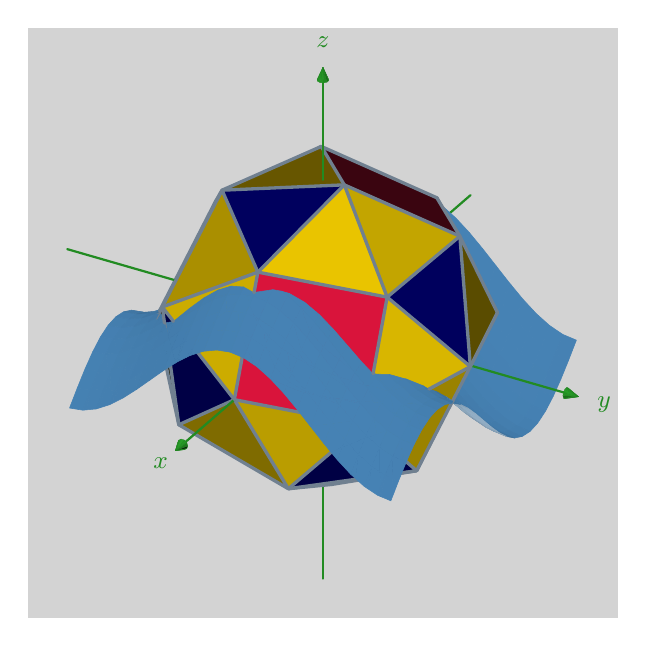
\begin{tikzpicture}%
\pgfsetxvec{\pgfxy(0.75,0)}%
\pgfsetyvec{\pgfxy(0,0.75)}%
\useasboundingbox (-5,-5)--(5,5);
%objet1  (User)
\pgfsetstrokecolor{rgb,1:red,0;green,0;blue,0}%
\pgfsetlinewidth{0.4pt}%
\pgfsetroundjoin%
\pgfpathmoveto{\pgfxy(-5,5)}%
\pgfpathlineto{\pgfxy(-5,-5)}\pgfpathlineto{\pgfxy(5,-5)}\pgfpathlineto{\pgfxy(5,5)}\pgfclosepath%
\pgfsetfillcolor{rgb,1:red,0.8275;green,0.8275;blue,0.8275}%
\pgffill%
\pgfsetstrokecolor{rgb,1:red,0.2353;green,0.4392;blue,0.6118}%
\pgfsetlinewidth{0.2pt}%
\pgfpathmoveto{\pgfxy(2.6599,-1.6768)}%
\pgfpathlineto{\pgfxy(2.529,-1.6108)}\pgfpathlineto{\pgfxy(2.7558,-1.7628)}\pgfpathlineto{\pgfxy(2.8867,-1.8287)}\pgfclosepath%
\pgfsetfillcolor{rgb,1:red,0.2353;green,0.4392;blue,0.6118}%
\pgffillstroke%
\pgfsetstrokecolor{rgb,1:red,0.2745;green,0.5098;blue,0.7059}%
\pgfpathmoveto{\pgfxy(3.0298,0.3371)}%
\pgfpathlineto{\pgfxy(3.2537,0.0662)}\pgfpathlineto{\pgfxy(3.3846,0.4037)}\pgfpathlineto{\pgfxy(3.1865,0.6435)}\pgfclosepath%
\pgfsetfillcolor{rgb,1:red,0.2745;green,0.5098;blue,0.7059}%
\pgffillstroke%
\pgfpathmoveto{\pgfxy(3.3846,0.4037)}%
\pgfpathlineto{\pgfxy(3.2537,0.0662)}\pgfpathlineto{\pgfxy(3.4804,-0.1786)}\pgfpathlineto{\pgfxy(3.6113,0.1589)}\pgfclosepath%
\pgfsetfillcolor{rgb,1:red,0.2745;green,0.5098;blue,0.7059}%
\pgffillstroke%
\pgfpathmoveto{\pgfxy(3.4804,-0.1786)}%
\pgfpathlineto{\pgfxy(3.3495,-0.5008)}\pgfpathlineto{\pgfxy(3.5762,-0.7039)}\pgfpathlineto{\pgfxy(3.7071,-0.3817)}\pgfclosepath%
\pgfsetfillcolor{rgb,1:red,0.2745;green,0.5098;blue,0.7059}%
\pgffillstroke%
\pgfpathmoveto{\pgfxy(3.6113,0.1589)}%
\pgfpathlineto{\pgfxy(3.4804,-0.1786)}\pgfpathlineto{\pgfxy(3.7071,-0.3817)}\pgfpathlineto{\pgfxy(3.838,-0.0441)}\pgfclosepath%
\pgfsetfillcolor{rgb,1:red,0.2745;green,0.5098;blue,0.7059}%
\pgffillstroke%
\pgfpathmoveto{\pgfxy(3.009,0.2963)}%
\pgfpathlineto{\pgfxy(2.8961,0.0183)}\pgfpathlineto{\pgfxy(3.1228,-0.256)}\pgfpathlineto{\pgfxy(3.2537,0.0662)}\pgfpathlineto{\pgfxy(3.0298,0.3371)}%
\pgfclosepath%
\pgfsetfillcolor{rgb,1:red,0.2745;green,0.5098;blue,0.7059}%
\pgffillstroke%
\pgfpathmoveto{\pgfxy(3.2537,0.0662)}%
\pgfpathlineto{\pgfxy(3.1228,-0.256)}\pgfpathlineto{\pgfxy(3.3495,-0.5008)}\pgfpathlineto{\pgfxy(3.4804,-0.1786)}\pgfclosepath%
\pgfsetfillcolor{rgb,1:red,0.2745;green,0.5098;blue,0.7059}%
\pgffillstroke%
\pgfpathmoveto{\pgfxy(3.838,-0.0441)}%
\pgfpathlineto{\pgfxy(3.7071,-0.3817)}\pgfpathlineto{\pgfxy(3.9339,-0.5336)}\pgfpathlineto{\pgfxy(4.0648,-0.1961)}\pgfclosepath%
\pgfsetfillcolor{rgb,1:red,0.2745;green,0.5098;blue,0.7059}%
\pgffillstroke%
\pgfpathmoveto{\pgfxy(2.8785,0.0408)}%
\pgfpathlineto{\pgfxy(2.8961,0.0183)}\pgfpathlineto{\pgfxy(3.009,0.2963)}\pgfclosepath%
\pgfsetfillcolor{rgb,1:red,0.2745;green,0.5098;blue,0.7059}%
\pgffillstroke%
\pgfpathmoveto{\pgfxy(2.8961,0.0183)}%
\pgfpathlineto{\pgfxy(2.7652,-0.2744)}\pgfpathlineto{\pgfxy(2.9919,-0.5487)}\pgfpathlineto{\pgfxy(3.1228,-0.256)}\pgfclosepath%
\pgfsetfillcolor{rgb,1:red,0.2745;green,0.5098;blue,0.7059}%
\pgffillstroke%
\pgfpathmoveto{\pgfxy(3.7071,-0.3817)}%
\pgfpathlineto{\pgfxy(3.5762,-0.7039)}\pgfpathlineto{\pgfxy(3.803,-0.8559)}\pgfpathlineto{\pgfxy(3.9339,-0.5336)}\pgfclosepath%
\pgfsetfillcolor{rgb,1:red,0.2745;green,0.5098;blue,0.7059}%
\pgffillstroke%
\pgfsetstrokecolor{rgb,1:red,0.2745;green,0.5059;blue,0.702}%
\pgfpathmoveto{\pgfxy(4.0648,-0.1961)}%
\pgfpathlineto{\pgfxy(3.9339,-0.5336)}\pgfpathlineto{\pgfxy(4.1606,-0.6286)}\pgfpathlineto{\pgfxy(4.2915,-0.2911)}\pgfclosepath%
\pgfsetfillcolor{rgb,1:red,0.2745;green,0.5059;blue,0.702}%
\pgffillstroke%
\pgfsetstrokecolor{rgb,1:red,0.2745;green,0.5098;blue,0.7059}%
\pgfpathmoveto{\pgfxy(3.1228,-0.256)}%
\pgfpathlineto{\pgfxy(2.9919,-0.5487)}\pgfpathlineto{\pgfxy(3.2186,-0.7935)}\pgfpathlineto{\pgfxy(3.3495,-0.5008)}\pgfclosepath%
\pgfsetfillcolor{rgb,1:red,0.2745;green,0.5098;blue,0.7059}%
\pgffillstroke%
\pgfsetstrokecolor{rgb,1:red,0.2745;green,0.5098;blue,0.702}%
\pgfpathmoveto{\pgfxy(2.7363,-0.2376)}%
\pgfpathlineto{\pgfxy(2.7652,-0.2744)}\pgfpathlineto{\pgfxy(2.8961,0.0183)}\pgfpathlineto{\pgfxy(2.8785,0.0408)}\pgfclosepath%
\pgfsetfillcolor{rgb,1:red,0.2745;green,0.5098;blue,0.702}%
\pgffillstroke%
\pgfsetstrokecolor{rgb,1:red,0.2745;green,0.5098;blue,0.7059}%
\pgfpathmoveto{\pgfxy(3.3495,-0.5008)}%
\pgfpathlineto{\pgfxy(3.2186,-0.7935)}\pgfpathlineto{\pgfxy(3.4453,-0.9966)}\pgfpathlineto{\pgfxy(3.5762,-0.7039)}\pgfclosepath%
\pgfsetfillcolor{rgb,1:red,0.2745;green,0.5098;blue,0.7059}%
\pgffillstroke%
\pgfsetstrokecolor{rgb,1:red,0.2745;green,0.5059;blue,0.702}%
\pgfpathmoveto{\pgfxy(3.803,-0.8559)}%
\pgfpathlineto{\pgfxy(3.6721,-1.1486)}\pgfpathlineto{\pgfxy(3.8988,-1.2435)}\pgfpathlineto{\pgfxy(4.0297,-0.9508)}\pgfclosepath%
\pgfsetfillcolor{rgb,1:red,0.2745;green,0.5059;blue,0.702}%
\pgffillstroke%
\pgfpathmoveto{\pgfxy(3.9339,-0.5336)}%
\pgfpathlineto{\pgfxy(3.803,-0.8559)}\pgfpathlineto{\pgfxy(4.0297,-0.9508)}\pgfpathlineto{\pgfxy(4.1606,-0.6286)}\pgfclosepath%
\pgfsetfillcolor{rgb,1:red,0.2745;green,0.5059;blue,0.702}%
\pgffillstroke%
\pgfsetstrokecolor{rgb,1:red,0.2745;green,0.5098;blue,0.702}%
\pgfpathmoveto{\pgfxy(3.5762,-0.7039)}%
\pgfpathlineto{\pgfxy(3.4453,-0.9966)}\pgfpathlineto{\pgfxy(3.6721,-1.1486)}\pgfpathlineto{\pgfxy(3.803,-0.8559)}\pgfclosepath%
\pgfsetfillcolor{rgb,1:red,0.2745;green,0.5098;blue,0.702}%
\pgffillstroke%
\pgfsetstrokecolor{rgb,1:red,0.2745;green,0.5059;blue,0.702}%
\pgfpathmoveto{\pgfxy(2.7652,-0.2744)}%
\pgfpathlineto{\pgfxy(2.6343,-0.5254)}\pgfpathlineto{\pgfxy(2.861,-0.7997)}\pgfpathlineto{\pgfxy(2.9919,-0.5487)}\pgfclosepath%
\pgfsetfillcolor{rgb,1:red,0.2745;green,0.5059;blue,0.702}%
\pgffillstroke%
\pgfpathmoveto{\pgfxy(2.6072,-0.4909)}%
\pgfpathlineto{\pgfxy(2.6343,-0.5254)}\pgfpathlineto{\pgfxy(2.7652,-0.2744)}\pgfpathlineto{\pgfxy(2.7363,-0.2376)}\pgfclosepath%
\pgfsetfillcolor{rgb,1:red,0.2745;green,0.5059;blue,0.702}%
\pgffillstroke%
\pgfpathmoveto{\pgfxy(2.9919,-0.5487)}%
\pgfpathlineto{\pgfxy(2.861,-0.7997)}\pgfpathlineto{\pgfxy(3.0877,-1.0445)}\pgfpathlineto{\pgfxy(3.2186,-0.7935)}\pgfclosepath%
\pgfsetfillcolor{rgb,1:red,0.2745;green,0.5059;blue,0.702}%
\pgffillstroke%
\pgfpathmoveto{\pgfxy(3.2186,-0.7935)}%
\pgfpathlineto{\pgfxy(3.0877,-1.0445)}\pgfpathlineto{\pgfxy(3.3144,-1.2476)}\pgfpathlineto{\pgfxy(3.4453,-0.9966)}\pgfclosepath%
\pgfsetfillcolor{rgb,1:red,0.2745;green,0.5059;blue,0.702}%
\pgffillstroke%
\pgfsetstrokecolor{rgb,1:red,0.2706;green,0.5059;blue,0.698}%
\pgfpathmoveto{\pgfxy(2.6343,-0.5254)}%
\pgfpathlineto{\pgfxy(2.5034,-0.7253)}\pgfpathlineto{\pgfxy(2.7301,-0.9996)}\pgfpathlineto{\pgfxy(2.861,-0.7997)}\pgfclosepath%
\pgfsetfillcolor{rgb,1:red,0.2706;green,0.5059;blue,0.698}%
\pgffillstroke%
\pgfsetstrokecolor{rgb,1:red,0.2745;green,0.5059;blue,0.702}%
\pgfpathmoveto{\pgfxy(3.4453,-0.9966)}%
\pgfpathlineto{\pgfxy(3.3144,-1.2476)}\pgfpathlineto{\pgfxy(3.5412,-1.3996)}\pgfpathlineto{\pgfxy(3.6721,-1.1486)}\pgfclosepath%
\pgfsetfillcolor{rgb,1:red,0.2745;green,0.5059;blue,0.702}%
\pgffillstroke%
\pgfsetstrokecolor{rgb,1:red,0.2706;green,0.5059;blue,0.702}%
\pgfpathmoveto{\pgfxy(3.6721,-1.1486)}%
\pgfpathlineto{\pgfxy(3.5412,-1.3996)}\pgfpathlineto{\pgfxy(3.7679,-1.4945)}\pgfpathlineto{\pgfxy(3.8988,-1.2435)}\pgfclosepath%
\pgfsetfillcolor{rgb,1:red,0.2706;green,0.5059;blue,0.702}%
\pgffillstroke%
\pgfsetstrokecolor{rgb,1:red,0.2706;green,0.5059;blue,0.698}%
\pgfpathmoveto{\pgfxy(2.494,-0.7134)}%
\pgfpathlineto{\pgfxy(2.5034,-0.7253)}\pgfpathlineto{\pgfxy(2.6343,-0.5254)}\pgfpathlineto{\pgfxy(2.6072,-0.4909)}\pgfclosepath%
\pgfsetfillcolor{rgb,1:red,0.2706;green,0.5059;blue,0.698}%
\pgffillstroke%
\pgfsetstrokecolor{rgb,1:red,0.2706;green,0.5059;blue,0.702}%
\pgfpathmoveto{\pgfxy(2.861,-0.7997)}%
\pgfpathlineto{\pgfxy(2.7301,-0.9996)}\pgfpathlineto{\pgfxy(2.9568,-1.2444)}\pgfpathlineto{\pgfxy(3.0877,-1.0445)}\pgfclosepath%
\pgfsetfillcolor{rgb,1:red,0.2706;green,0.5059;blue,0.702}%
\pgffillstroke%
\pgfpathmoveto{\pgfxy(3.0877,-1.0445)}%
\pgfpathlineto{\pgfxy(2.9568,-1.2444)}\pgfpathlineto{\pgfxy(3.1835,-1.4475)}\pgfpathlineto{\pgfxy(3.3144,-1.2476)}\pgfclosepath%
\pgfsetfillcolor{rgb,1:red,0.2706;green,0.5059;blue,0.702}%
\pgffillstroke%
\pgfsetstrokecolor{rgb,1:red,0.2706;green,0.5059;blue,0.698}%
\pgfpathmoveto{\pgfxy(3.3144,-1.2476)}%
\pgfpathlineto{\pgfxy(3.1835,-1.4475)}\pgfpathlineto{\pgfxy(3.4103,-1.5994)}\pgfpathlineto{\pgfxy(3.5412,-1.3996)}\pgfclosepath%
\pgfsetfillcolor{rgb,1:red,0.2706;green,0.5059;blue,0.698}%
\pgffillstroke%
\pgfsetstrokecolor{rgb,1:red,0.2706;green,0.502;blue,0.698}%
\pgfpathmoveto{\pgfxy(3.5412,-1.3996)}%
\pgfpathlineto{\pgfxy(3.4103,-1.5994)}\pgfpathlineto{\pgfxy(3.637,-1.6944)}\pgfpathlineto{\pgfxy(3.7679,-1.4945)}\pgfclosepath%
\pgfsetfillcolor{rgb,1:red,0.2706;green,0.502;blue,0.698}%
\pgffillstroke%
\pgfsetstrokecolor{rgb,1:red,0.2706;green,0.502;blue,0.6941}%
\pgfpathmoveto{\pgfxy(2.469,-0.7628)}%
\pgfpathlineto{\pgfxy(2.5034,-0.7253)}\pgfpathlineto{\pgfxy(2.494,-0.7134)}\pgfclosepath%
\pgfsetfillcolor{rgb,1:red,0.2706;green,0.502;blue,0.6941}%
\pgffillstroke%
\pgfpathmoveto{\pgfxy(2.7301,-0.9996)}%
\pgfpathlineto{\pgfxy(2.5992,-1.1425)}\pgfpathlineto{\pgfxy(2.8259,-1.3873)}\pgfpathlineto{\pgfxy(2.9568,-1.2444)}\pgfclosepath%
\pgfsetfillcolor{rgb,1:red,0.2706;green,0.502;blue,0.6941}%
\pgffillstroke%
\pgfpathmoveto{\pgfxy(2.5034,-0.7253)}%
\pgfpathlineto{\pgfxy(2.469,-0.7628)}\pgfpathlineto{\pgfxy(2.3992,-0.9005)}\pgfpathlineto{\pgfxy(2.5992,-1.1425)}\pgfpathlineto{\pgfxy(2.7301,-0.9996)}%
\pgfclosepath%
\pgfsetfillcolor{rgb,1:red,0.2706;green,0.502;blue,0.6941}%
\pgffillstroke%
\pgfpathmoveto{\pgfxy(2.9568,-1.2444)}%
\pgfpathlineto{\pgfxy(2.8259,-1.3873)}\pgfpathlineto{\pgfxy(3.0526,-1.5903)}\pgfpathlineto{\pgfxy(3.1835,-1.4475)}\pgfclosepath%
\pgfsetfillcolor{rgb,1:red,0.2706;green,0.502;blue,0.6941}%
\pgffillstroke%
\pgfsetstrokecolor{rgb,1:red,0.2667;green,0.498;blue,0.6902}%
\pgfpathmoveto{\pgfxy(3.4103,-1.5994)}%
\pgfpathlineto{\pgfxy(3.2794,-1.7423)}\pgfpathlineto{\pgfxy(3.5061,-1.8373)}\pgfpathlineto{\pgfxy(3.637,-1.6944)}\pgfclosepath%
\pgfsetfillcolor{rgb,1:red,0.2667;green,0.498;blue,0.6902}%
\pgffillstroke%
\pgfsetstrokecolor{rgb,1:red,0.2706;green,0.502;blue,0.6941}%
\pgfpathmoveto{\pgfxy(3.1835,-1.4475)}%
\pgfpathlineto{\pgfxy(3.0526,-1.5903)}\pgfpathlineto{\pgfxy(3.2794,-1.7423)}\pgfpathlineto{\pgfxy(3.4103,-1.5994)}\pgfclosepath%
\pgfsetfillcolor{rgb,1:red,0.2706;green,0.502;blue,0.6941}%
\pgffillstroke%
\pgfsetstrokecolor{rgb,1:red,0.2667;green,0.498;blue,0.6863}%
\pgfpathmoveto{\pgfxy(2.3233,-1.0509)}%
\pgfpathlineto{\pgfxy(2.4683,-1.2263)}\pgfpathlineto{\pgfxy(2.5992,-1.1425)}\pgfpathlineto{\pgfxy(2.3992,-0.9005)}\pgfclosepath%
\pgfsetfillcolor{rgb,1:red,0.2667;green,0.498;blue,0.6863}%
\pgffillstroke%
\pgfpathmoveto{\pgfxy(2.5992,-1.1425)}%
\pgfpathlineto{\pgfxy(2.4683,-1.2263)}\pgfpathlineto{\pgfxy(2.695,-1.4711)}\pgfpathlineto{\pgfxy(2.8259,-1.3873)}\pgfclosepath%
\pgfsetfillcolor{rgb,1:red,0.2667;green,0.498;blue,0.6863}%
\pgffillstroke%
\pgfsetstrokecolor{rgb,1:red,0.2667;green,0.4941;blue,0.6863}%
\pgfpathmoveto{\pgfxy(2.8259,-1.3873)}%
\pgfpathlineto{\pgfxy(2.695,-1.4711)}\pgfpathlineto{\pgfxy(2.9217,-1.6742)}\pgfpathlineto{\pgfxy(3.0526,-1.5903)}\pgfclosepath%
\pgfsetfillcolor{rgb,1:red,0.2667;green,0.4941;blue,0.6863}%
\pgffillstroke%
\pgfsetstrokecolor{rgb,1:red,0.2667;green,0.4941;blue,0.6824}%
\pgfpathmoveto{\pgfxy(3.0526,-1.5903)}%
\pgfpathlineto{\pgfxy(2.9217,-1.6742)}\pgfpathlineto{\pgfxy(3.1485,-1.8262)}\pgfpathlineto{\pgfxy(3.2794,-1.7423)}\pgfclosepath%
\pgfsetfillcolor{rgb,1:red,0.2667;green,0.4941;blue,0.6824}%
\pgffillstroke%
\pgfsetstrokecolor{rgb,1:red,0.2627;green,0.4902;blue,0.6784}%
\pgfpathmoveto{\pgfxy(3.2794,-1.7423)}%
\pgfpathlineto{\pgfxy(3.1485,-1.8262)}\pgfpathlineto{\pgfxy(3.3752,-1.9211)}\pgfpathlineto{\pgfxy(3.5061,-1.8373)}\pgfclosepath%
\pgfsetfillcolor{rgb,1:red,0.2627;green,0.4902;blue,0.6784}%
\pgffillstroke%
\pgfpathmoveto{\pgfxy(2.2656,-1.1663)}%
\pgfpathlineto{\pgfxy(2.3374,-1.2532)}\pgfpathlineto{\pgfxy(2.4683,-1.2263)}\pgfpathlineto{\pgfxy(2.3233,-1.0509)}\pgfclosepath%
\pgfsetfillcolor{rgb,1:red,0.2627;green,0.4902;blue,0.6784}%
\pgffillstroke%
\pgfsetstrokecolor{rgb,1:red,0.2627;green,0.4863;blue,0.6745}%
\pgfpathmoveto{\pgfxy(2.4683,-1.2263)}%
\pgfpathlineto{\pgfxy(2.3374,-1.2532)}\pgfpathlineto{\pgfxy(2.5641,-1.498)}\pgfpathlineto{\pgfxy(2.695,-1.4711)}\pgfclosepath%
\pgfsetfillcolor{rgb,1:red,0.2627;green,0.4863;blue,0.6745}%
\pgffillstroke%
\pgfpathmoveto{\pgfxy(2.695,-1.4711)}%
\pgfpathlineto{\pgfxy(2.5641,-1.498)}\pgfpathlineto{\pgfxy(2.7908,-1.701)}\pgfpathlineto{\pgfxy(2.9217,-1.6742)}\pgfclosepath%
\pgfsetfillcolor{rgb,1:red,0.2627;green,0.4863;blue,0.6745}%
\pgffillstroke%
\pgfsetstrokecolor{rgb,1:red,0.2588;green,0.4824;blue,0.6667}%
\pgfpathmoveto{\pgfxy(2.9217,-1.6742)}%
\pgfpathlineto{\pgfxy(2.7908,-1.701)}\pgfpathlineto{\pgfxy(3.0176,-1.853)}\pgfpathlineto{\pgfxy(3.1485,-1.8262)}\pgfclosepath%
\pgfsetfillcolor{rgb,1:red,0.2588;green,0.4824;blue,0.6667}%
\pgffillstroke%
\pgfsetstrokecolor{rgb,1:red,0.2549;green,0.4745;blue,0.6588}%
\pgfpathmoveto{\pgfxy(3.1485,-1.8262)}%
\pgfpathlineto{\pgfxy(3.0176,-1.853)}\pgfpathlineto{\pgfxy(3.2443,-1.948)}\pgfpathlineto{\pgfxy(3.3752,-1.9211)}\pgfclosepath%
\pgfsetfillcolor{rgb,1:red,0.2549;green,0.4745;blue,0.6588}%
\pgffillstroke%
\pgfsetstrokecolor{rgb,1:red,0.2588;green,0.4784;blue,0.6627}%
\pgfpathmoveto{\pgfxy(2.3374,-1.2532)}%
\pgfpathlineto{\pgfxy(2.2323,-1.2337)}\pgfpathlineto{\pgfxy(2.2249,-1.2488)}\pgfpathlineto{\pgfxy(2.4332,-1.4737)}\pgfpathlineto{\pgfxy(2.5641,-1.498)}%
\pgfclosepath%
\pgfsetfillcolor{rgb,1:red,0.2588;green,0.4784;blue,0.6627}%
\pgffillstroke%
\pgfpathmoveto{\pgfxy(2.2323,-1.2337)}%
\pgfpathlineto{\pgfxy(2.3374,-1.2532)}\pgfpathlineto{\pgfxy(2.2656,-1.1663)}\pgfclosepath%
\pgfsetfillcolor{rgb,1:red,0.2588;green,0.4784;blue,0.6627}%
\pgffillstroke%
\pgfsetstrokecolor{rgb,1:red,0.2549;green,0.4745;blue,0.6549}%
\pgfpathmoveto{\pgfxy(2.5641,-1.498)}%
\pgfpathlineto{\pgfxy(2.4332,-1.4737)}\pgfpathlineto{\pgfxy(2.6599,-1.6768)}\pgfpathlineto{\pgfxy(2.7908,-1.701)}\pgfclosepath%
\pgfsetfillcolor{rgb,1:red,0.2549;green,0.4745;blue,0.6549}%
\pgffillstroke%
\pgfsetstrokecolor{rgb,1:red,0.251;green,0.4667;blue,0.6471}%
\pgfpathmoveto{\pgfxy(2.7908,-1.701)}%
\pgfpathlineto{\pgfxy(2.6599,-1.6768)}\pgfpathlineto{\pgfxy(2.8867,-1.8287)}\pgfpathlineto{\pgfxy(3.0176,-1.853)}\pgfclosepath%
\pgfsetfillcolor{rgb,1:red,0.251;green,0.4667;blue,0.6471}%
\pgffillstroke%
\pgfsetstrokecolor{rgb,1:red,0.2431;green,0.451;blue,0.6235}%
\pgfpathmoveto{\pgfxy(3.0176,-1.853)}%
\pgfpathlineto{\pgfxy(2.8867,-1.8287)}\pgfpathlineto{\pgfxy(3.1134,-1.9237)}\pgfpathlineto{\pgfxy(3.2443,-1.948)}\pgfclosepath%
\pgfsetfillcolor{rgb,1:red,0.2431;green,0.451;blue,0.6235}%
\pgffillstroke%
\pgfsetstrokecolor{rgb,1:red,0.251;green,0.4667;blue,0.6471}%
\pgfpathmoveto{\pgfxy(2.2012,-1.2985)}%
\pgfpathlineto{\pgfxy(2.3023,-1.4077)}\pgfpathlineto{\pgfxy(2.4332,-1.4737)}\pgfpathlineto{\pgfxy(2.2249,-1.2488)}\pgfclosepath%
\pgfsetfillcolor{rgb,1:red,0.251;green,0.4667;blue,0.6471}%
\pgffillstroke%
\pgfsetstrokecolor{rgb,1:red,0.2471;green,0.4588;blue,0.6353}%
\pgfpathmoveto{\pgfxy(2.4332,-1.4737)}%
\pgfpathlineto{\pgfxy(2.3023,-1.4077)}\pgfpathlineto{\pgfxy(2.529,-1.6108)}\pgfpathlineto{\pgfxy(2.6599,-1.6768)}\pgfclosepath%
\pgfsetfillcolor{rgb,1:red,0.2471;green,0.4588;blue,0.6353}%
\pgffillstroke%
\pgfsetstrokecolor{rgb,1:red,0.2431;green,0.4549;blue,0.6275}%
\pgfpathmoveto{\pgfxy(2.1892,-1.3251)}%
\pgfpathlineto{\pgfxy(2.3023,-1.4077)}\pgfpathlineto{\pgfxy(2.2012,-1.2985)}\pgfclosepath%
\pgfsetfillcolor{rgb,1:red,0.2431;green,0.4549;blue,0.6275}%
\pgffillstroke%
\pgfsetstrokecolor{rgb,1:red,0.2353;green,0.4392;blue,0.6078}%
\pgfpathmoveto{\pgfxy(2.3023,-1.4077)}%
\pgfpathlineto{\pgfxy(2.1883,-1.3273)}\pgfpathlineto{\pgfxy(2.3981,-1.5153)}\pgfpathlineto{\pgfxy(2.529,-1.6108)}\pgfclosepath%
\pgfsetfillcolor{rgb,1:red,0.2353;green,0.4392;blue,0.6078}%
\pgffillstroke%
\pgfsetstrokecolor{rgb,1:red,0.2235;green,0.4118;blue,0.5686}%
\pgfpathmoveto{\pgfxy(2.1874,-1.333)}%
\pgfpathlineto{\pgfxy(2.2672,-1.4045)}\pgfpathlineto{\pgfxy(2.3981,-1.5153)}\pgfpathlineto{\pgfxy(2.1883,-1.3273)}\pgfclosepath%
\pgfsetfillcolor{rgb,1:red,0.2235;green,0.4118;blue,0.5686}%
\pgffillstroke%
\pgfpathmoveto{\pgfxy(2.1869,-1.3365)}%
\pgfpathlineto{\pgfxy(2.2672,-1.4045)}\pgfpathlineto{\pgfxy(2.1874,-1.333)}\pgfclosepath%
\pgfsetfillcolor{rgb,1:red,0.2235;green,0.4118;blue,0.5686}%
\pgffillstroke%
\pgfsetstrokecolor{rgb,1:red,0.5647;green,0.7686;blue,0.5647}%
\pgfsetlinewidth{0.1pt}%
\pgfpathmoveto{\pgfxy(4.1291,-1.2565)}%
\pgfpathlineto{\pgfxy(4.1541,-1.2034)}\pgfpathlineto{\pgfxy(4.3301,-1.25)}\pgfclosepath%
\pgfsetfillcolor{rgb,1:red,0.6314;green,0.8627;blue,0.6314}%
\pgffillstroke%
\pgfpathmoveto{\pgfxy(4.1541,-1.2034)}%
\pgfpathlineto{\pgfxy(4.1636,-1.1442)}\pgfpathlineto{\pgfxy(4.3301,-1.25)}\pgfclosepath%
\pgfsetfillcolor{rgb,1:red,0.5922;green,0.8039;blue,0.5922}%
\pgffillstroke%
\pgfpathmoveto{\pgfxy(4.1636,-1.1442)}%
\pgfpathlineto{\pgfxy(4.1541,-1.1016)}\pgfpathlineto{\pgfxy(4.3301,-1.25)}\pgfclosepath%
\pgfsetfillcolor{rgb,1:red,0.4314;green,0.5882;blue,0.4314}%
\pgffillstroke%
\pgfpathmoveto{\pgfxy(4.0982,-1.2832)}%
\pgfpathlineto{\pgfxy(4.1291,-1.2565)}\pgfpathlineto{\pgfxy(4.3301,-1.25)}\pgfclosepath%
\pgfsetfillcolor{rgb,1:red,0.5843;green,0.7961;blue,0.5843}%
\pgffillstroke%
\pgfsetstrokecolor{rgb,1:red,0.1333;green,0.5451;blue,0.1333}%
\pgfsetlinewidth{0.8pt}%
\pgfsetroundcap%
\pgfxyline(4.1136,-1.1875)(2.5034,-0.7227)%
\pgfsetlinewidth{0.1pt}%
\pgfpathmoveto{\pgfxy(4.0732,-1.1716)}%
\pgfpathlineto{\pgfxy(4.0636,-1.2308)}\pgfpathlineto{\pgfxy(4.3301,-1.25)}\pgfclosepath%
\pgfsetfillcolor{rgb,1:red,0.1412;green,0.5725;blue,0.1412}%
\pgffillstroke%
\pgfpathmoveto{\pgfxy(4.0982,-1.1185)}%
\pgfpathlineto{\pgfxy(4.0732,-1.1716)}\pgfpathlineto{\pgfxy(4.3301,-1.25)}\pgfclosepath%
\pgfsetfillcolor{rgb,1:red,0.149;green,0.6157;blue,0.149}%
\pgffillstroke%
\pgfpathmoveto{\pgfxy(4.1291,-1.0918)}%
\pgfpathlineto{\pgfxy(4.0982,-1.1185)}\pgfpathlineto{\pgfxy(4.3301,-1.25)}\pgfclosepath%
\pgfsetfillcolor{rgb,1:red,0.1373;green,0.5686;blue,0.1373}%
\pgffillstroke%
\pgfpathmoveto{\pgfxy(4.0732,-1.2734)}%
\pgfpathlineto{\pgfxy(4.0982,-1.2832)}\pgfpathlineto{\pgfxy(4.3301,-1.25)}\pgfclosepath%
\pgfsetfillcolor{rgb,1:red,0.098;green,0.4039;blue,0.098}%
\pgffillstroke%
\pgfpathmoveto{\pgfxy(4.0636,-1.2308)}%
\pgfpathlineto{\pgfxy(4.0732,-1.2734)}\pgfpathlineto{\pgfxy(4.3301,-1.25)}\pgfclosepath%
\pgfsetfillcolor{rgb,1:red,0.102;green,0.4235;blue,0.102}%
\pgffillstroke%
\pgfpathmoveto{\pgfxy(4.1541,-1.1016)}%
\pgfpathlineto{\pgfxy(4.1291,-1.0918)}\pgfpathlineto{\pgfxy(4.3301,-1.25)}\pgfclosepath%
\pgfsetfillcolor{rgb,1:red,0.102;green,0.4078;blue,0.102}%
\pgffillstroke%
\pgfsetlinewidth{0.3pt}%
\pgfputat{\pgfxy(4.7631,-1.375)}{\pgftext{\color{rgb,1:red,0.1333;green,0.5451;blue,0.1333}\small $y$}}\pgfstroke%
\pgfsetstrokecolor{rgb,1:red,0.5725;green,0.6784;blue,0.7686}%
\pgfsetlinewidth{0.2pt}%
\pgfpathmoveto{\pgfxy(2.494,-1.5565)}%
\pgfpathlineto{\pgfxy(2.3631,-1.4457)}\pgfpathlineto{\pgfxy(2.5898,-1.5406)}\pgfpathlineto{\pgfxy(2.7207,-1.6514)}\pgfclosepath%
\pgfsetfillcolor{rgb,1:red,0.5725;green,0.6784;blue,0.7686}%
\pgffillstroke%
\pgfsetstrokecolor{rgb,1:red,0.549;green,0.651;blue,0.7333}%
\pgfpathmoveto{\pgfxy(2.2672,-1.4045)}%
\pgfpathlineto{\pgfxy(2.1869,-1.3365)}\pgfpathlineto{\pgfxy(2.1909,-1.3302)}\pgfpathlineto{\pgfxy(2.3631,-1.4457)}\pgfpathlineto{\pgfxy(2.494,-1.5565)}%
\pgfclosepath%
\pgfsetfillcolor{rgb,1:red,0.549;green,0.651;blue,0.7333}%
\pgffillstroke%
\pgfpathmoveto{\pgfxy(2.3981,-1.5153)}%
\pgfpathlineto{\pgfxy(2.2672,-1.4045)}\pgfpathlineto{\pgfxy(2.494,-1.5565)}\pgfpathlineto{\pgfxy(2.6249,-1.6672)}\pgfclosepath%
\pgfsetfillcolor{rgb,1:red,0.549;green,0.651;blue,0.7333}%
\pgffillstroke%
\pgfsetstrokecolor{rgb,1:red,0.5216;green,0.6157;blue,0.698}%
\pgfpathmoveto{\pgfxy(2.3631,-1.4457)}%
\pgfpathlineto{\pgfxy(2.1909,-1.3302)}\pgfpathlineto{\pgfxy(2.1948,-1.3261)}\pgfclosepath%
\pgfsetfillcolor{rgb,1:red,0.5216;green,0.6157;blue,0.698}%
\pgffillstroke%
\pgfsetstrokecolor{rgb,1:red,0.5725;green,0.6784;blue,0.7686}%
\pgfpathmoveto{\pgfxy(2.6249,-1.6672)}%
\pgfpathlineto{\pgfxy(2.494,-1.5565)}\pgfpathlineto{\pgfxy(2.7207,-1.6514)}\pgfpathlineto{\pgfxy(2.8516,-1.7622)}\pgfclosepath%
\pgfsetfillcolor{rgb,1:red,0.5725;green,0.6784;blue,0.7686}%
\pgffillstroke%
\pgfsetstrokecolor{rgb,1:red,0.5647;green,0.6706;blue,0.7569}%
\pgfpathmoveto{\pgfxy(2.3631,-1.4457)}%
\pgfpathlineto{\pgfxy(2.2322,-1.3502)}\pgfpathlineto{\pgfxy(2.4589,-1.4451)}\pgfpathlineto{\pgfxy(2.5898,-1.5406)}\pgfclosepath%
\pgfsetfillcolor{rgb,1:red,0.5647;green,0.6706;blue,0.7569}%
\pgffillstroke%
\pgfsetstrokecolor{rgb,1:red,0.5333;green,0.6314;blue,0.7137}%
\pgfpathmoveto{\pgfxy(2.2322,-1.3502)}%
\pgfpathlineto{\pgfxy(2.2186,-1.3333)}\pgfpathlineto{\pgfxy(2.328,-1.3791)}\pgfpathlineto{\pgfxy(2.4589,-1.4451)}\pgfclosepath%
\pgfsetfillcolor{rgb,1:red,0.5333;green,0.6314;blue,0.7137}%
\pgffillstroke%
\pgfsetstrokecolor{rgb,1:red,0.2431;green,0.451;blue,0.6235}%
\pgfpathmoveto{\pgfxy(2.328,-1.3791)}%
\pgfpathlineto{\pgfxy(2.2209,-1.3347)}\pgfclosepath%
\pgfsetfillcolor{rgb,1:red,0.2431;green,0.451;blue,0.6235}%
\pgffillstroke%
\pgfsetstrokecolor{rgb,1:red,0.5216;green,0.6157;blue,0.698}%
\pgfpathmoveto{\pgfxy(2.1953,-1.3255)}%
\pgfpathlineto{\pgfxy(2.2322,-1.3502)}\pgfpathlineto{\pgfxy(2.3631,-1.4457)}\pgfclosepath%
\pgfsetfillcolor{rgb,1:red,0.5216;green,0.6157;blue,0.698}%
\pgffillstroke%
\pgfsetstrokecolor{rgb,1:red,0.2353;green,0.4392;blue,0.6118}%
\pgfpathmoveto{\pgfxy(2.1933,-1.3306)}%
\pgfpathlineto{\pgfxy(2.2322,-1.3502)}\pgfpathlineto{\pgfxy(2.1953,-1.3255)}\pgfclosepath%
\pgfsetfillcolor{rgb,1:red,0.2353;green,0.4392;blue,0.6118}%
\pgffillstroke%
\pgfsetstrokecolor{rgb,1:red,0.5333;green,0.6314;blue,0.7137}%
\pgfpathmoveto{\pgfxy(2.2322,-1.3502)}%
\pgfpathlineto{\pgfxy(2.1933,-1.3306)}\pgfpathlineto{\pgfxy(2.1978,-1.3246)}\pgfpathlineto{\pgfxy(2.2186,-1.3333)}\pgfclosepath%
\pgfsetfillcolor{rgb,1:red,0.5333;green,0.6314;blue,0.7137}%
\pgffillstroke%
\pgfsetstrokecolor{rgb,1:red,0.2431;green,0.451;blue,0.6235}%
\pgfpathmoveto{\pgfxy(2.2186,-1.3333)}%
\pgfpathlineto{\pgfxy(2.1977,-1.325)}\pgfclosepath%
\pgfsetfillcolor{rgb,1:red,0.2431;green,0.451;blue,0.6235}%
\pgffillstroke%
\pgfsetstrokecolor{rgb,1:red,0.5647;green,0.6706;blue,0.7569}%
\pgfpathmoveto{\pgfxy(2.7558,-1.7628)}%
\pgfpathlineto{\pgfxy(2.6249,-1.6672)}\pgfpathlineto{\pgfxy(2.8516,-1.7622)}\pgfpathlineto{\pgfxy(2.9825,-1.8577)}\pgfclosepath%
\pgfsetfillcolor{rgb,1:red,0.5647;green,0.6706;blue,0.7569}%
\pgffillstroke%
\pgfsetstrokecolor{rgb,1:red,0.2431;green,0.451;blue,0.6235}%
\pgfpathmoveto{\pgfxy(2.2213,-1.3594)}%
\pgfpathlineto{\pgfxy(2.3261,-1.3788)}\pgfpathlineto{\pgfxy(2.1977,-1.325)}\pgfpathlineto{\pgfxy(2.1909,-1.3405)}\pgfclosepath%
\pgfsetfillcolor{rgb,1:red,0.2431;green,0.451;blue,0.6235}%
\pgffillstroke%
\pgfsetstrokecolor{rgb,1:red,0.5216;green,0.6157;blue,0.698}%
\pgfpathmoveto{\pgfxy(2.529,-1.6108)}%
\pgfpathlineto{\pgfxy(2.3981,-1.5153)}\pgfpathlineto{\pgfxy(2.6249,-1.6672)}\pgfpathlineto{\pgfxy(2.7558,-1.7628)}\pgfclosepath%
\pgfsetfillcolor{rgb,1:red,0.5216;green,0.6157;blue,0.698}%
\pgffillstroke%
\pgfsetstrokecolor{rgb,1:red,0.2549;green,0.4745;blue,0.6588}%
\pgfpathmoveto{\pgfxy(2.1829,-1.3578)}%
\pgfpathlineto{\pgfxy(2.1971,-1.3549)}\pgfpathlineto{\pgfxy(2.1865,-1.3504)}\pgfclosepath%
\pgfsetfillcolor{rgb,1:red,0.2549;green,0.4745;blue,0.6588}%
\pgffillstroke%
\pgfsetstrokecolor{rgb,1:red,0.2431;green,0.451;blue,0.6235}%
\pgfpathmoveto{\pgfxy(2.1865,-1.3504)}%
\pgfpathlineto{\pgfxy(2.1971,-1.3549)}\pgfpathlineto{\pgfxy(2.2213,-1.3594)}\pgfpathlineto{\pgfxy(2.1909,-1.3405)}\pgfclosepath%
\pgfsetfillcolor{rgb,1:red,0.2431;green,0.451;blue,0.6235}%
\pgffillstroke%
\pgfsetstrokecolor{rgb,1:red,0.5333;green,0.6314;blue,0.7137}%
\pgfpathmoveto{\pgfxy(2.8867,-1.8287)}%
\pgfpathlineto{\pgfxy(2.7558,-1.7628)}\pgfpathlineto{\pgfxy(2.9825,-1.8577)}\pgfpathlineto{\pgfxy(3.1134,-1.9237)}\pgfclosepath%
\pgfsetfillcolor{rgb,1:red,0.5333;green,0.6314;blue,0.7137}%
\pgffillstroke%
\pgfsetstrokecolor{rgb,1:red,0.0118;green,0;blue,0.0039}%
\pgfpathmoveto{\pgfxy(2.044,-1.5879)}%
\pgfpathlineto{\pgfxy(2.9538,0.1759)}\pgfpathlineto{\pgfxy(2.4965,-0.7389)}\pgfpathlineto{\pgfxy(1.5867,-2.5027)}\pgfclosepath%
\pgfsetfillcolor{rgb,1:red,0.0118;green,0;blue,0.0039}%
\pgffillstroke%
\pgfsetstrokecolor{rgb,1:red,0.1333;green,0.5451;blue,0.1333}%
\pgfsetlinewidth{0.8pt}%
\pgfxyline(2.5,2.1651)(1.5,1.299)%
\pgfsetstrokecolor{rgb,1:red,0.2588;green,0.4784;blue,0.6627}%
\pgfsetlinewidth{0.2pt}%
\pgfpathmoveto{\pgfxy(-0.7666,0.2475)}%
\pgfpathlineto{\pgfxy(-0.8975,0.0476)}\pgfpathlineto{\pgfxy(-0.6708,0.191)}\pgfpathlineto{\pgfxy(-0.5399,0.3909)}\pgfclosepath%
\pgfsetfillcolor{rgb,1:red,0.2588;green,0.4784;blue,0.6627}%
\pgffillstroke%
\pgfsetstrokecolor{rgb,1:red,0.2667;green,0.4941;blue,0.6824}%
\pgfpathmoveto{\pgfxy(-0.7315,0.6773)}%
\pgfpathlineto{\pgfxy(-0.8624,0.3846)}\pgfpathlineto{\pgfxy(-0.6357,0.4985)}\pgfpathlineto{\pgfxy(-0.5048,0.7912)}\pgfclosepath%
\pgfsetfillcolor{rgb,1:red,0.2667;green,0.4941;blue,0.6824}%
\pgffillstroke%
\pgfsetstrokecolor{rgb,1:red,0.2706;green,0.498;blue,0.6941}%
\pgfpathmoveto{\pgfxy(-1.6735,0.0763)}%
\pgfpathlineto{\pgfxy(-1.8044,-0.1236)}\pgfpathlineto{\pgfxy(-1.5777,-0.1595)}\pgfpathlineto{\pgfxy(-1.4468,0.0403)}\pgfclosepath%
\pgfsetfillcolor{rgb,1:red,0.2706;green,0.498;blue,0.6941}%
\pgffillstroke%
\pgfsetstrokecolor{rgb,1:red,0.2706;green,0.5059;blue,0.698}%
\pgfpathmoveto{\pgfxy(-1.4117,0.62)}%
\pgfpathlineto{\pgfxy(-1.5426,0.3273)}\pgfpathlineto{\pgfxy(-1.3159,0.2913)}\pgfpathlineto{\pgfxy(-1.185,0.584)}\pgfclosepath%
\pgfsetfillcolor{rgb,1:red,0.2706;green,0.5059;blue,0.698}%
\pgffillstroke%
\pgfpathmoveto{\pgfxy(-1.2808,0.9422)}%
\pgfpathlineto{\pgfxy(-1.4117,0.62)}\pgfpathlineto{\pgfxy(-1.185,0.584)}\pgfpathlineto{\pgfxy(-1.0541,0.9063)}\pgfclosepath%
\pgfsetfillcolor{rgb,1:red,0.2706;green,0.5059;blue,0.698}%
\pgffillstroke%
\pgfpathmoveto{\pgfxy(-1.1499,1.2797)}%
\pgfpathlineto{\pgfxy(-1.2808,0.9422)}\pgfpathlineto{\pgfxy(-1.0541,0.9063)}\pgfpathlineto{\pgfxy(-0.9232,1.2438)}\pgfclosepath%
\pgfsetfillcolor{rgb,1:red,0.2706;green,0.5059;blue,0.698}%
\pgffillstroke%
\pgfsetstrokecolor{rgb,1:red,0.2706;green,0.502;blue,0.6941}%
\pgfpathmoveto{\pgfxy(-0.9232,1.2438)}%
\pgfpathlineto{\pgfxy(-1.0541,0.9063)}\pgfpathlineto{\pgfxy(-0.8274,0.9273)}\pgfpathlineto{\pgfxy(-0.6965,1.2648)}\pgfclosepath%
\pgfsetfillcolor{rgb,1:red,0.2706;green,0.502;blue,0.6941}%
\pgffillstroke%
\pgfsetstrokecolor{rgb,1:red,0.2706;green,0.502;blue,0.698}%
\pgfpathmoveto{\pgfxy(-1.5426,0.3273)}%
\pgfpathlineto{\pgfxy(-1.6735,0.0763)}\pgfpathlineto{\pgfxy(-1.4468,0.0403)}\pgfpathlineto{\pgfxy(-1.3159,0.2913)}\pgfclosepath%
\pgfsetfillcolor{rgb,1:red,0.2706;green,0.502;blue,0.698}%
\pgffillstroke%
\pgfsetstrokecolor{rgb,1:red,0.2706;green,0.502;blue,0.6941}%
\pgfpathmoveto{\pgfxy(-1.0541,0.9063)}%
\pgfpathlineto{\pgfxy(-1.185,0.584)}\pgfpathlineto{\pgfxy(-0.9583,0.6051)}\pgfpathlineto{\pgfxy(-0.8274,0.9273)}\pgfclosepath%
\pgfsetfillcolor{rgb,1:red,0.2706;green,0.502;blue,0.6941}%
\pgffillstroke%
\pgfpathmoveto{\pgfxy(-1.185,0.584)}%
\pgfpathlineto{\pgfxy(-1.3159,0.2913)}\pgfpathlineto{\pgfxy(-1.0892,0.3124)}\pgfpathlineto{\pgfxy(-0.9583,0.6051)}\pgfclosepath%
\pgfsetfillcolor{rgb,1:red,0.2706;green,0.502;blue,0.6941}%
\pgffillstroke%
\pgfsetstrokecolor{rgb,1:red,0.2667;green,0.498;blue,0.6902}%
\pgfpathmoveto{\pgfxy(-0.6965,1.2648)}%
\pgfpathlineto{\pgfxy(-0.8274,0.9273)}\pgfpathlineto{\pgfxy(-0.6006,0.9995)}\pgfpathlineto{\pgfxy(-0.4697,1.337)}\pgfclosepath%
\pgfsetfillcolor{rgb,1:red,0.2667;green,0.498;blue,0.6902}%
\pgffillstroke%
\pgfsetstrokecolor{rgb,1:red,0.2667;green,0.4941;blue,0.6863}%
\pgfpathmoveto{\pgfxy(-0.4697,1.337)}%
\pgfpathlineto{\pgfxy(-0.6006,0.9995)}\pgfpathlineto{\pgfxy(-0.3739,1.1134)}\pgfpathlineto{\pgfxy(-0.243,1.4509)}\pgfclosepath%
\pgfsetfillcolor{rgb,1:red,0.2667;green,0.4941;blue,0.6863}%
\pgffillstroke%
\pgfsetstrokecolor{rgb,1:red,0.2667;green,0.498;blue,0.6902}%
\pgfpathmoveto{\pgfxy(-1.3159,0.2913)}%
\pgfpathlineto{\pgfxy(-1.4468,0.0403)}\pgfpathlineto{\pgfxy(-1.2201,0.0614)}\pgfpathlineto{\pgfxy(-1.0892,0.3124)}\pgfclosepath%
\pgfsetfillcolor{rgb,1:red,0.2667;green,0.498;blue,0.6902}%
\pgffillstroke%
\pgfpathmoveto{\pgfxy(-0.8274,0.9273)}%
\pgfpathlineto{\pgfxy(-0.9583,0.6051)}\pgfpathlineto{\pgfxy(-0.7315,0.6773)}\pgfpathlineto{\pgfxy(-0.6006,0.9995)}\pgfclosepath%
\pgfsetfillcolor{rgb,1:red,0.2667;green,0.498;blue,0.6902}%
\pgffillstroke%
\pgfsetstrokecolor{rgb,1:red,0.2667;green,0.498;blue,0.6863}%
\pgfpathmoveto{\pgfxy(-0.9583,0.6051)}%
\pgfpathlineto{\pgfxy(-1.0892,0.3124)}\pgfpathlineto{\pgfxy(-0.8624,0.3846)}\pgfpathlineto{\pgfxy(-0.7315,0.6773)}\pgfclosepath%
\pgfsetfillcolor{rgb,1:red,0.2667;green,0.498;blue,0.6863}%
\pgffillstroke%
\pgfsetstrokecolor{rgb,1:red,0.2667;green,0.4941;blue,0.6824}%
\pgfpathmoveto{\pgfxy(-1.8044,-0.1236)}%
\pgfpathlineto{\pgfxy(-1.9353,-0.2665)}\pgfpathlineto{\pgfxy(-1.7086,-0.3024)}\pgfpathlineto{\pgfxy(-1.5777,-0.1595)}\pgfclosepath%
\pgfsetfillcolor{rgb,1:red,0.2667;green,0.4941;blue,0.6824}%
\pgffillstroke%
\pgfsetstrokecolor{rgb,1:red,0.2667;green,0.4941;blue,0.6863}%
\pgfpathmoveto{\pgfxy(-1.4468,0.0403)}%
\pgfpathlineto{\pgfxy(-1.5777,-0.1595)}\pgfpathlineto{\pgfxy(-1.351,-0.1385)}\pgfpathlineto{\pgfxy(-1.2201,0.0614)}\pgfclosepath%
\pgfsetfillcolor{rgb,1:red,0.2667;green,0.4941;blue,0.6863}%
\pgffillstroke%
\pgfsetstrokecolor{rgb,1:red,0.2667;green,0.4941;blue,0.6824}%
\pgfpathmoveto{\pgfxy(-1.0892,0.3124)}%
\pgfpathlineto{\pgfxy(-1.2201,0.0614)}\pgfpathlineto{\pgfxy(-0.9933,0.1336)}\pgfpathlineto{\pgfxy(-0.8624,0.3846)}\pgfclosepath%
\pgfsetfillcolor{rgb,1:red,0.2667;green,0.4941;blue,0.6824}%
\pgffillstroke%
\pgfsetstrokecolor{rgb,1:red,0.2667;green,0.4941;blue,0.6863}%
\pgfpathmoveto{\pgfxy(-0.6006,0.9995)}%
\pgfpathlineto{\pgfxy(-0.7315,0.6773)}\pgfpathlineto{\pgfxy(-0.5048,0.7912)}\pgfpathlineto{\pgfxy(-0.3739,1.1134)}\pgfclosepath%
\pgfsetfillcolor{rgb,1:red,0.2667;green,0.4941;blue,0.6863}%
\pgffillstroke%
\pgfsetstrokecolor{rgb,1:red,0.2706;green,0.502;blue,0.6941}%
\pgfpathmoveto{\pgfxy(1.1054,2.2104)}%
\pgfpathlineto{\pgfxy(1.088,2.1655)}\pgfpathlineto{\pgfxy(1.1663,2.2458)}\pgfpathlineto{\pgfxy(1.1249,2.242)}\pgfclosepath%
\pgfsetfillcolor{rgb,1:red,0.2706;green,0.502;blue,0.6941}%
\pgffillstroke%
\pgfsetstrokecolor{rgb,1:red,0.2667;green,0.498;blue,0.6902}%
\pgfpathmoveto{\pgfxy(0.9606,2.0077)}%
\pgfpathlineto{\pgfxy(1.088,2.1655)}\pgfpathlineto{\pgfxy(1.1054,2.2104)}\pgfclosepath%
\pgfsetfillcolor{rgb,1:red,0.2667;green,0.498;blue,0.6902}%
\pgffillstroke%
\pgfsetstrokecolor{rgb,1:red,0.2627;green,0.4902;blue,0.6784}%
\pgfpathmoveto{\pgfxy(-0.5048,0.7912)}%
\pgfpathlineto{\pgfxy(-0.6357,0.4985)}\pgfpathlineto{\pgfxy(-0.409,0.6419)}\pgfpathlineto{\pgfxy(-0.2781,0.9346)}\pgfclosepath%
\pgfsetfillcolor{rgb,1:red,0.2627;green,0.4902;blue,0.6784}%
\pgffillstroke%
\pgfsetstrokecolor{rgb,1:red,0.2706;green,0.502;blue,0.6941}%
\pgfpathmoveto{\pgfxy(1.1173,2.2412)}%
\pgfpathlineto{\pgfxy(1.1054,2.2104)}\pgfpathlineto{\pgfxy(1.1249,2.242)}\pgfclosepath%
\pgfsetfillcolor{rgb,1:red,0.2706;green,0.502;blue,0.6941}%
\pgffillstroke%
\pgfsetstrokecolor{rgb,1:red,0.2667;green,0.498;blue,0.6902}%
\pgfpathmoveto{\pgfxy(0.763,1.8326)}%
\pgfpathlineto{\pgfxy(0.8388,1.8567)}\pgfpathlineto{\pgfxy(0.9606,2.0077)}\pgfpathlineto{\pgfxy(1.1054,2.2104)}\pgfpathlineto{\pgfxy(1.1173,2.2412)}%
\pgfpathlineto{\pgfxy(0.8939,2.1701)}\pgfclosepath%
\pgfsetfillcolor{rgb,1:red,0.2667;green,0.498;blue,0.6902}%
\pgffillstroke%
\pgfpathmoveto{\pgfxy(0.7379,1.7387)}%
\pgfpathlineto{\pgfxy(0.8388,1.8567)}\pgfpathlineto{\pgfxy(0.763,1.8326)}\pgfclosepath%
\pgfsetfillcolor{rgb,1:red,0.2667;green,0.498;blue,0.6902}%
\pgffillstroke%
\pgfsetstrokecolor{rgb,1:red,0.2667;green,0.4941;blue,0.6824}%
\pgfpathmoveto{\pgfxy(-0.243,1.4509)}%
\pgfpathlineto{\pgfxy(-0.3739,1.1134)}\pgfpathlineto{\pgfxy(-0.1472,1.2568)}\pgfpathlineto{\pgfxy(-0.0163,1.5944)}\pgfclosepath%
\pgfsetfillcolor{rgb,1:red,0.2667;green,0.4941;blue,0.6824}%
\pgffillstroke%
\pgfsetstrokecolor{rgb,1:red,0.2627;green,0.4902;blue,0.6745}%
\pgfpathmoveto{\pgfxy(-1.2201,0.0614)}%
\pgfpathlineto{\pgfxy(-1.351,-0.1385)}\pgfpathlineto{\pgfxy(-1.1242,-0.0663)}\pgfpathlineto{\pgfxy(-0.9933,0.1336)}\pgfclosepath%
\pgfsetfillcolor{rgb,1:red,0.2627;green,0.4902;blue,0.6745}%
\pgffillstroke%
\pgfsetstrokecolor{rgb,1:red,0.2627;green,0.4863;blue,0.6745}%
\pgfpathmoveto{\pgfxy(-1.5777,-0.1595)}%
\pgfpathlineto{\pgfxy(-1.7086,-0.3024)}\pgfpathlineto{\pgfxy(-1.4819,-0.2814)}\pgfpathlineto{\pgfxy(-1.351,-0.1385)}\pgfclosepath%
\pgfsetfillcolor{rgb,1:red,0.2627;green,0.4863;blue,0.6745}%
\pgffillstroke%
\pgfsetstrokecolor{rgb,1:red,0.2588;green,0.4824;blue,0.6706}%
\pgfpathmoveto{\pgfxy(-1.9353,-0.2665)}%
\pgfpathlineto{\pgfxy(-2.0662,-0.3503)}\pgfpathlineto{\pgfxy(-1.8395,-0.3863)}\pgfpathlineto{\pgfxy(-1.7086,-0.3024)}\pgfclosepath%
\pgfsetfillcolor{rgb,1:red,0.2588;green,0.4824;blue,0.6706}%
\pgffillstroke%
\pgfsetstrokecolor{rgb,1:red,0.2667;green,0.498;blue,0.6902}%
\pgfpathmoveto{\pgfxy(0.7132,1.7099)}%
\pgfpathlineto{\pgfxy(0.7379,1.7387)}\pgfpathlineto{\pgfxy(0.763,1.8326)}\pgfclosepath%
\pgfsetfillcolor{rgb,1:red,0.2667;green,0.498;blue,0.6902}%
\pgffillstroke%
\pgfsetstrokecolor{rgb,1:red,0.2627;green,0.4902;blue,0.6824}%
\pgfpathmoveto{\pgfxy(-0.3739,1.1134)}%
\pgfpathlineto{\pgfxy(-0.5048,0.7912)}\pgfpathlineto{\pgfxy(-0.2781,0.9346)}\pgfpathlineto{\pgfxy(-0.1472,1.2568)}\pgfclosepath%
\pgfsetfillcolor{rgb,1:red,0.2627;green,0.4902;blue,0.6824}%
\pgffillstroke%
\pgfsetstrokecolor{rgb,1:red,0.2627;green,0.4902;blue,0.6784}%
\pgfpathmoveto{\pgfxy(-0.8624,0.3846)}%
\pgfpathlineto{\pgfxy(-0.9933,0.1336)}\pgfpathlineto{\pgfxy(-0.7666,0.2475)}\pgfpathlineto{\pgfxy(-0.6357,0.4985)}\pgfclosepath%
\pgfsetfillcolor{rgb,1:red,0.2627;green,0.4902;blue,0.6784}%
\pgffillstroke%
\pgfsetstrokecolor{rgb,1:red,0.2588;green,0.4784;blue,0.6627}%
\pgfpathmoveto{\pgfxy(-1.351,-0.1385)}%
\pgfpathlineto{\pgfxy(-1.4819,-0.2814)}\pgfpathlineto{\pgfxy(-1.2551,-0.2092)}\pgfpathlineto{\pgfxy(-1.1242,-0.0663)}\pgfclosepath%
\pgfsetfillcolor{rgb,1:red,0.2588;green,0.4784;blue,0.6627}%
\pgffillstroke%
\pgfsetstrokecolor{rgb,1:red,0.2549;green,0.4745;blue,0.6549}%
\pgfpathmoveto{\pgfxy(-1.7086,-0.3024)}%
\pgfpathlineto{\pgfxy(-1.8395,-0.3863)}\pgfpathlineto{\pgfxy(-1.6128,-0.3652)}\pgfpathlineto{\pgfxy(-1.4819,-0.2814)}\pgfclosepath%
\pgfsetfillcolor{rgb,1:red,0.2549;green,0.4745;blue,0.6549}%
\pgffillstroke%
\pgfsetstrokecolor{rgb,1:red,0.2627;green,0.4863;blue,0.6706}%
\pgfpathmoveto{\pgfxy(-0.6357,0.4985)}%
\pgfpathlineto{\pgfxy(-0.7666,0.2475)}\pgfpathlineto{\pgfxy(-0.5399,0.3909)}\pgfpathlineto{\pgfxy(-0.409,0.6419)}\pgfclosepath%
\pgfsetfillcolor{rgb,1:red,0.2627;green,0.4863;blue,0.6706}%
\pgffillstroke%
\pgfsetstrokecolor{rgb,1:red,0.251;green,0.4627;blue,0.6392}%
\pgfpathmoveto{\pgfxy(-2.0662,-0.3503)}%
\pgfpathlineto{\pgfxy(-2.1971,-0.3772)}\pgfpathlineto{\pgfxy(-1.9704,-0.4131)}\pgfpathlineto{\pgfxy(-1.8395,-0.3863)}\pgfclosepath%
\pgfsetfillcolor{rgb,1:red,0.251;green,0.4627;blue,0.6392}%
\pgffillstroke%
\pgfsetstrokecolor{rgb,1:red,0.2588;green,0.4824;blue,0.6667}%
\pgfpathmoveto{\pgfxy(-0.9933,0.1336)}%
\pgfpathlineto{\pgfxy(-1.1242,-0.0663)}\pgfpathlineto{\pgfxy(-0.8975,0.0476)}\pgfpathlineto{\pgfxy(-0.7666,0.2475)}\pgfclosepath%
\pgfsetfillcolor{rgb,1:red,0.2588;green,0.4824;blue,0.6667}%
\pgffillstroke%
\pgfsetstrokecolor{rgb,1:red,0.2667;green,0.498;blue,0.6902}%
\pgfpathmoveto{\pgfxy(0.7597,1.8316)}%
\pgfpathlineto{\pgfxy(0.763,1.8326)}\pgfpathlineto{\pgfxy(0.7683,1.8461)}\pgfclosepath%
\pgfsetfillcolor{rgb,1:red,0.2667;green,0.498;blue,0.6902}%
\pgffillstroke%
\pgfpathmoveto{\pgfxy(0.7597,1.8316)}%
\pgfpathlineto{\pgfxy(0.7077,1.7035)}\pgfpathlineto{\pgfxy(0.7132,1.7099)}\pgfpathlineto{\pgfxy(0.763,1.8326)}\pgfclosepath%
\pgfsetfillcolor{rgb,1:red,0.2667;green,0.498;blue,0.6902}%
\pgffillstroke%
\pgfsetstrokecolor{rgb,1:red,0.2667;green,0.4941;blue,0.6863}%
\pgfpathmoveto{\pgfxy(0.533,1.7177)}%
\pgfpathlineto{\pgfxy(0.5203,1.4548)}\pgfpathlineto{\pgfxy(0.7077,1.7035)}\pgfpathlineto{\pgfxy(0.7597,1.8316)}\pgfclosepath%
\pgfsetfillcolor{rgb,1:red,0.2667;green,0.4941;blue,0.6863}%
\pgffillstroke%
\pgfsetstrokecolor{rgb,1:red,0.2667;green,0.498;blue,0.6902}%
\pgfpathmoveto{\pgfxy(0.8906,2.1691)}%
\pgfpathlineto{\pgfxy(0.7597,1.8316)}\pgfpathlineto{\pgfxy(0.7683,1.8461)}\pgfpathlineto{\pgfxy(0.8939,2.1701)}\pgfclosepath%
\pgfsetfillcolor{rgb,1:red,0.2667;green,0.498;blue,0.6902}%
\pgffillstroke%
\pgfsetstrokecolor{rgb,1:red,0.2667;green,0.4941;blue,0.6863}%
\pgfpathmoveto{\pgfxy(0.6639,2.0552)}%
\pgfpathlineto{\pgfxy(0.533,1.7177)}\pgfpathlineto{\pgfxy(0.7597,1.8316)}\pgfpathlineto{\pgfxy(0.8906,2.1691)}\pgfclosepath%
\pgfsetfillcolor{rgb,1:red,0.2667;green,0.4941;blue,0.6863}%
\pgffillstroke%
\pgfsetstrokecolor{rgb,1:red,0.2667;green,0.4941;blue,0.6824}%
\pgfpathmoveto{\pgfxy(0.4372,1.9117)}%
\pgfpathlineto{\pgfxy(0.3063,1.5742)}\pgfpathlineto{\pgfxy(0.533,1.7177)}\pgfpathlineto{\pgfxy(0.6639,2.0552)}\pgfclosepath%
\pgfsetfillcolor{rgb,1:red,0.2667;green,0.4941;blue,0.6824}%
\pgffillstroke%
\pgfsetstrokecolor{rgb,1:red,0.2667;green,0.4941;blue,0.6863}%
\pgfpathmoveto{\pgfxy(0.533,1.7177)}%
\pgfpathlineto{\pgfxy(0.4021,1.3954)}\pgfpathlineto{\pgfxy(0.5195,1.4544)}\pgfclosepath%
\pgfsetfillcolor{rgb,1:red,0.2667;green,0.4941;blue,0.6863}%
\pgffillstroke%
\pgfsetstrokecolor{rgb,1:red,0.2667;green,0.4941;blue,0.6824}%
\pgfpathmoveto{\pgfxy(0.4021,1.3954)}%
\pgfpathlineto{\pgfxy(0.4289,1.3454)}\pgfpathlineto{\pgfxy(0.5195,1.4544)}\pgfclosepath%
\pgfsetfillcolor{rgb,1:red,0.2667;green,0.4941;blue,0.6824}%
\pgffillstroke%
\pgfsetstrokecolor{rgb,1:red,0.2627;green,0.4902;blue,0.6824}%
\pgfpathmoveto{\pgfxy(0.3063,1.5742)}%
\pgfpathlineto{\pgfxy(0.4021,1.3954)}\pgfpathlineto{\pgfxy(0.533,1.7177)}\pgfclosepath%
\pgfsetfillcolor{rgb,1:red,0.2627;green,0.4902;blue,0.6824}%
\pgffillstroke%
\pgfsetstrokecolor{rgb,1:red,0.2627;green,0.4902;blue,0.6784}%
\pgfpathmoveto{\pgfxy(-0.0163,1.5944)}%
\pgfpathlineto{\pgfxy(-0.1472,1.2568)}\pgfpathlineto{\pgfxy(0.0795,1.4155)}\pgfpathlineto{\pgfxy(0.2104,1.753)}\pgfclosepath%
\pgfsetfillcolor{rgb,1:red,0.2627;green,0.4902;blue,0.6784}%
\pgffillstroke%
\pgfsetstrokecolor{rgb,1:red,0.2471;green,0.4588;blue,0.6353}%
\pgfpathmoveto{\pgfxy(-1.4819,-0.2814)}%
\pgfpathlineto{\pgfxy(-1.6128,-0.3652)}\pgfpathlineto{\pgfxy(-1.386,-0.293)}\pgfpathlineto{\pgfxy(-1.2551,-0.2092)}\pgfclosepath%
\pgfsetfillcolor{rgb,1:red,0.2471;green,0.4588;blue,0.6353}%
\pgffillstroke%
\pgfsetstrokecolor{rgb,1:red,0.2627;green,0.4902;blue,0.6824}%
\pgfpathmoveto{\pgfxy(0.3063,1.5742)}%
\pgfpathlineto{\pgfxy(0.1754,1.252)}\pgfpathlineto{\pgfxy(0.4021,1.3954)}\pgfclosepath%
\pgfsetfillcolor{rgb,1:red,0.2627;green,0.4902;blue,0.6824}%
\pgffillstroke%
\pgfsetstrokecolor{rgb,1:red,0.2667;green,0.4941;blue,0.6824}%
\pgfpathmoveto{\pgfxy(0.4021,1.3954)}%
\pgfpathlineto{\pgfxy(0.3343,1.2439)}\pgfpathlineto{\pgfxy(0.3353,1.2331)}\pgfpathlineto{\pgfxy(0.4289,1.3454)}\pgfclosepath%
\pgfsetfillcolor{rgb,1:red,0.2667;green,0.4941;blue,0.6824}%
\pgffillstroke%
\pgfsetstrokecolor{rgb,1:red,0.2627;green,0.4902;blue,0.6784}%
\pgfpathmoveto{\pgfxy(0.1754,1.252)}%
\pgfpathlineto{\pgfxy(0.3343,1.2439)}\pgfpathlineto{\pgfxy(0.4021,1.3954)}\pgfclosepath%
\pgfsetfillcolor{rgb,1:red,0.2627;green,0.4902;blue,0.6784}%
\pgffillstroke%
\pgfpathmoveto{\pgfxy(-0.1472,1.2568)}%
\pgfpathlineto{\pgfxy(-0.2781,0.9346)}\pgfpathlineto{\pgfxy(-0.0514,1.0933)}\pgfpathlineto{\pgfxy(0.0795,1.4155)}\pgfclosepath%
\pgfsetfillcolor{rgb,1:red,0.2627;green,0.4902;blue,0.6784}%
\pgffillstroke%
\pgfsetstrokecolor{rgb,1:red,0.2549;green,0.4706;blue,0.651}%
\pgfpathmoveto{\pgfxy(-1.1242,-0.0663)}%
\pgfpathlineto{\pgfxy(-1.2551,-0.2092)}\pgfpathlineto{\pgfxy(-1.0284,-0.0953)}\pgfpathlineto{\pgfxy(-0.8975,0.0476)}\pgfclosepath%
\pgfsetfillcolor{rgb,1:red,0.2549;green,0.4706;blue,0.651}%
\pgffillstroke%
\pgfsetstrokecolor{rgb,1:red,0.2353;green,0.4353;blue,0.6039}%
\pgfpathmoveto{\pgfxy(-1.8395,-0.3863)}%
\pgfpathlineto{\pgfxy(-1.9704,-0.4131)}\pgfpathlineto{\pgfxy(-1.7806,-0.3955)}\pgfpathlineto{\pgfxy(-1.7321,-0.3897)}\pgfpathlineto{\pgfxy(-1.6128,-0.3652)}%
\pgfclosepath%
\pgfsetfillcolor{rgb,1:red,0.2353;green,0.4353;blue,0.6039}%
\pgffillstroke%
\pgfsetstrokecolor{rgb,1:red,0.2471;green,0.4588;blue,0.6353}%
\pgfpathmoveto{\pgfxy(-0.6708,0.191)}%
\pgfpathlineto{\pgfxy(-0.7689,0.0839)}\pgfpathlineto{\pgfxy(-0.4853,0.3208)}\pgfclosepath%
\pgfsetfillcolor{rgb,1:red,0.2471;green,0.4588;blue,0.6353}%
\pgffillstroke%
\pgfsetstrokecolor{rgb,1:red,0.2549;green,0.4745;blue,0.6588}%
\pgfpathmoveto{\pgfxy(-0.5399,0.3909)}%
\pgfpathlineto{\pgfxy(-0.6708,0.191)}\pgfpathlineto{\pgfxy(-0.4853,0.3208)}\pgfpathlineto{\pgfxy(-0.4196,0.3871)}\pgfpathlineto{\pgfxy(-0.3132,0.5496)}%
\pgfclosepath%
\pgfsetfillcolor{rgb,1:red,0.2549;green,0.4745;blue,0.6588}%
\pgffillstroke%
\pgfsetstrokecolor{rgb,1:red,0.2627;green,0.4902;blue,0.6784}%
\pgfpathmoveto{\pgfxy(0.0445,0.9593)}%
\pgfpathlineto{\pgfxy(0.1988,1.0569)}\pgfpathlineto{\pgfxy(0.3099,1.2015)}\pgfclosepath%
\pgfsetfillcolor{rgb,1:red,0.2627;green,0.4902;blue,0.6784}%
\pgffillstroke%
\pgfsetstrokecolor{rgb,1:red,0.2627;green,0.4863;blue,0.6706}%
\pgfpathmoveto{\pgfxy(0.0445,0.9593)}%
\pgfpathlineto{\pgfxy(-0.055,0.7686)}\pgfpathlineto{\pgfxy(0.1988,1.0569)}\pgfclosepath%
\pgfsetfillcolor{rgb,1:red,0.2627;green,0.4863;blue,0.6706}%
\pgffillstroke%
\pgfsetstrokecolor{rgb,1:red,0.2588;green,0.4824;blue,0.6706}%
\pgfpathmoveto{\pgfxy(-0.409,0.6419)}%
\pgfpathlineto{\pgfxy(-0.5399,0.3909)}\pgfpathlineto{\pgfxy(-0.3132,0.5496)}\pgfpathlineto{\pgfxy(-0.1823,0.8006)}\pgfclosepath%
\pgfsetfillcolor{rgb,1:red,0.2588;green,0.4824;blue,0.6706}%
\pgffillstroke%
\pgfsetstrokecolor{rgb,1:red,0.2627;green,0.4902;blue,0.6784}%
\pgfpathmoveto{\pgfxy(0.2104,1.753)}%
\pgfpathlineto{\pgfxy(0.0795,1.4155)}\pgfpathlineto{\pgfxy(0.3063,1.5742)}\pgfpathlineto{\pgfxy(0.4372,1.9117)}\pgfclosepath%
\pgfsetfillcolor{rgb,1:red,0.2627;green,0.4902;blue,0.6784}%
\pgffillstroke%
\pgfsetstrokecolor{rgb,1:red,0.2667;green,0.4941;blue,0.6824}%
\pgfpathmoveto{\pgfxy(0.3343,1.2439)}%
\pgfpathlineto{\pgfxy(0.3229,1.2184)}\pgfpathlineto{\pgfxy(0.3353,1.2331)}\pgfclosepath%
\pgfsetfillcolor{rgb,1:red,0.2667;green,0.4941;blue,0.6824}%
\pgffillstroke%
\pgfsetstrokecolor{rgb,1:red,0.2627;green,0.4902;blue,0.6784}%
\pgfpathmoveto{\pgfxy(0.1754,1.252)}%
\pgfpathlineto{\pgfxy(0.0445,0.9593)}\pgfpathlineto{\pgfxy(0.3099,1.2015)}\pgfpathlineto{\pgfxy(0.3229,1.2184)}\pgfpathlineto{\pgfxy(0.3343,1.2439)}%
\pgfclosepath%
\pgfsetfillcolor{rgb,1:red,0.2627;green,0.4902;blue,0.6784}%
\pgffillstroke%
\pgfsetstrokecolor{rgb,1:red,0.2627;green,0.4863;blue,0.6745}%
\pgfpathmoveto{\pgfxy(-0.2781,0.9346)}%
\pgfpathlineto{\pgfxy(-0.409,0.6419)}\pgfpathlineto{\pgfxy(-0.1823,0.8006)}\pgfpathlineto{\pgfxy(-0.0514,1.0933)}\pgfclosepath%
\pgfsetfillcolor{rgb,1:red,0.2627;green,0.4863;blue,0.6745}%
\pgffillstroke%
\pgfsetstrokecolor{rgb,1:red,0.2353;green,0.4392;blue,0.6039}%
\pgfpathmoveto{\pgfxy(-1.2551,-0.2092)}%
\pgfpathlineto{\pgfxy(-1.386,-0.293)}\pgfpathlineto{\pgfxy(-1.2884,-0.244)}\pgfpathlineto{\pgfxy(-1.1035,-0.1434)}\pgfpathlineto{\pgfxy(-1.0284,-0.0953)}%
\pgfclosepath%
\pgfsetfillcolor{rgb,1:red,0.2353;green,0.4392;blue,0.6039}%
\pgffillstroke%
\pgfsetstrokecolor{rgb,1:red,0.2627;green,0.4902;blue,0.6784}%
\pgfpathmoveto{\pgfxy(0.0795,1.4155)}%
\pgfpathlineto{\pgfxy(-0.0514,1.0933)}\pgfpathlineto{\pgfxy(0.1754,1.252)}\pgfpathlineto{\pgfxy(0.3063,1.5742)}\pgfclosepath%
\pgfsetfillcolor{rgb,1:red,0.2627;green,0.4902;blue,0.6784}%
\pgffillstroke%
\pgfsetstrokecolor{rgb,1:red,0.251;green,0.4627;blue,0.6392}%
\pgfpathmoveto{\pgfxy(-0.8975,0.0476)}%
\pgfpathlineto{\pgfxy(-1.0284,-0.0953)}\pgfpathlineto{\pgfxy(-0.8656,0.0077)}\pgfpathlineto{\pgfxy(-0.7689,0.0839)}\pgfpathlineto{\pgfxy(-0.6708,0.191)}%
\pgfclosepath%
\pgfsetfillcolor{rgb,1:red,0.251;green,0.4627;blue,0.6392}%
\pgffillstroke%
\pgfsetstrokecolor{rgb,1:red,0.2588;green,0.4824;blue,0.6706}%
\pgfpathmoveto{\pgfxy(-0.1823,0.8006)}%
\pgfpathlineto{\pgfxy(-0.3132,0.5496)}\pgfpathlineto{\pgfxy(-0.1337,0.6752)}\pgfpathlineto{\pgfxy(-0.055,0.7686)}\pgfpathlineto{\pgfxy(0.0445,0.9593)}%
\pgfclosepath%
\pgfsetfillcolor{rgb,1:red,0.2588;green,0.4824;blue,0.6706}%
\pgffillstroke%
\pgfsetstrokecolor{rgb,1:red,0.2627;green,0.4863;blue,0.6745}%
\pgfpathmoveto{\pgfxy(-0.0514,1.0933)}%
\pgfpathlineto{\pgfxy(-0.1823,0.8006)}\pgfpathlineto{\pgfxy(0.0445,0.9593)}\pgfpathlineto{\pgfxy(0.1754,1.252)}\pgfclosepath%
\pgfsetfillcolor{rgb,1:red,0.2627;green,0.4863;blue,0.6745}%
\pgffillstroke%
\pgfsetstrokecolor{rgb,1:red,0.2039;green,0.3765;blue,0.5255}%
\pgfpathmoveto{\pgfxy(-1.0284,-0.0953)}%
\pgfpathlineto{\pgfxy(-1.1035,-0.1434)}\pgfpathlineto{\pgfxy(-0.8656,0.0077)}\pgfclosepath%
\pgfsetfillcolor{rgb,1:red,0.2039;green,0.3765;blue,0.5255}%
\pgffillstroke%
\pgfsetstrokecolor{rgb,1:red,0.2549;green,0.4745;blue,0.6588}%
\pgfpathmoveto{\pgfxy(-0.3132,0.5496)}%
\pgfpathlineto{\pgfxy(-0.4196,0.3871)}\pgfpathlineto{\pgfxy(-0.1337,0.6752)}\pgfclosepath%
\pgfsetfillcolor{rgb,1:red,0.2549;green,0.4745;blue,0.6588}%
\pgffillstroke%
\pgfsetstrokecolor{rgb,1:red,0.5647;green,0.6706;blue,0.7569}%
\pgfpathmoveto{\pgfxy(-1.386,-0.293)}%
\pgfpathlineto{\pgfxy(-1.4245,-0.3009)}\pgfpathlineto{\pgfxy(-1.2884,-0.244)}\pgfclosepath%
\pgfsetfillcolor{rgb,1:red,0.5647;green,0.6706;blue,0.7569}%
\pgffillstroke%
\pgfpathmoveto{\pgfxy(-1.9704,-0.4131)}%
\pgfpathlineto{\pgfxy(-2.0251,-0.403)}\pgfpathlineto{\pgfxy(-1.7806,-0.3955)}\pgfclosepath%
\pgfsetfillcolor{rgb,1:red,0.5647;green,0.6706;blue,0.7569}%
\pgffillstroke%
\pgfsetstrokecolor{rgb,1:red,0.5412;green,0.6392;blue,0.7255}%
\pgfpathmoveto{\pgfxy(-1.6128,-0.3652)}%
\pgfpathlineto{\pgfxy(-1.7321,-0.3897)}\pgfpathlineto{\pgfxy(-1.4245,-0.3009)}\pgfpathlineto{\pgfxy(-1.386,-0.293)}\pgfclosepath%
\pgfsetfillcolor{rgb,1:red,0.5412;green,0.6392;blue,0.7255}%
\pgffillstroke%
\pgfsetstrokecolor{rgb,1:red,0.5059;green,0.5961;blue,0.6745}%
\pgfpathmoveto{\pgfxy(-2.1971,-0.3772)}%
\pgfpathlineto{\pgfxy(-2.3064,-0.3569)}\pgfpathlineto{\pgfxy(-2.0251,-0.403)}\pgfpathlineto{\pgfxy(-1.9704,-0.4131)}\pgfclosepath%
\pgfsetfillcolor{rgb,1:red,0.5059;green,0.5961;blue,0.6745}%
\pgffillstroke%
\pgfsetstrokecolor{rgb,1:red,0.851;green,0.0784;blue,0.2314}%
\pgfpathmoveto{\pgfxy(0.1578,1.9868)}%
\pgfpathlineto{\pgfxy(1.7792,0.4574)}\pgfpathlineto{\pgfxy(0.2549,-1.1247)}\pgfpathlineto{\pgfxy(-1.3664,0.4047)}\pgfclosepath%
\pgfsetfillcolor{rgb,1:red,0.851;green,0.0784;blue,0.2314}%
\pgffillstroke%
\pgfsetstrokecolor{rgb,1:red,0.1333;green,0.5451;blue,0.1333}%
\pgfsetlinewidth{0.8pt}%
\pgfxyline(0,-4.3301)(0,-2.5981)%
\pgfsetstrokecolor{rgb,1:red,0.2706;green,0.5059;blue,0.698}%
\pgfsetlinewidth{0.2pt}%
\pgfpathmoveto{\pgfxy(-4.1606,-1.1035)}%
\pgfpathlineto{\pgfxy(-4.2915,-1.441)}\pgfpathlineto{\pgfxy(-4.0648,-1.4769)}\pgfpathlineto{\pgfxy(-3.9339,-1.1394)}\pgfclosepath%
\pgfsetfillcolor{rgb,1:red,0.2706;green,0.5059;blue,0.698}%
\pgffillstroke%
\pgfsetstrokecolor{rgb,1:red,0.2706;green,0.502;blue,0.6941}%
\pgfpathmoveto{\pgfxy(-3.9339,-1.1394)}%
\pgfpathlineto{\pgfxy(-4.0648,-1.4769)}\pgfpathlineto{\pgfxy(-4.004,-1.4713)}\pgfclosepath%
\pgfsetfillcolor{rgb,1:red,0.2706;green,0.502;blue,0.6941}%
\pgffillstroke%
\pgfsetstrokecolor{rgb,1:red,0.2706;green,0.5059;blue,0.698}%
\pgfpathmoveto{\pgfxy(-4.0802,-0.9056)}%
\pgfpathlineto{\pgfxy(-4.1606,-1.1035)}\pgfpathlineto{\pgfxy(-3.9339,-1.1394)}\pgfpathlineto{\pgfxy(-3.8915,-1.0352)}\pgfclosepath%
\pgfsetfillcolor{rgb,1:red,0.2706;green,0.5059;blue,0.698}%
\pgffillstroke%
\pgfsetstrokecolor{rgb,1:red,0.2706;green,0.502;blue,0.6941}%
\pgfpathmoveto{\pgfxy(-3.9339,-1.1394)}%
\pgfpathlineto{\pgfxy(-4.004,-1.4713)}\pgfpathlineto{\pgfxy(-3.838,-1.4559)}\pgfpathlineto{\pgfxy(-3.7245,-1.1631)}\pgfpathlineto{\pgfxy(-3.7752,-1.1247)}%
\pgfclosepath%
\pgfsetfillcolor{rgb,1:red,0.2706;green,0.502;blue,0.6941}%
\pgffillstroke%
\pgfsetstrokecolor{rgb,1:red,0.2667;green,0.498;blue,0.6902}%
\pgfpathmoveto{\pgfxy(-3.7245,-1.1631)}%
\pgfpathlineto{\pgfxy(-3.838,-1.4559)}\pgfpathlineto{\pgfxy(-3.7703,-1.4343)}\pgfpathlineto{\pgfxy(-3.7173,-1.1692)}\pgfclosepath%
\pgfsetfillcolor{rgb,1:red,0.2667;green,0.498;blue,0.6902}%
\pgffillstroke%
\pgfsetstrokecolor{rgb,1:red,0.2706;green,0.502;blue,0.6941}%
\pgfpathmoveto{\pgfxy(-3.8915,-1.0352)}%
\pgfpathlineto{\pgfxy(-3.9339,-1.1394)}\pgfpathlineto{\pgfxy(-3.7752,-1.1247)}\pgfclosepath%
\pgfsetfillcolor{rgb,1:red,0.2706;green,0.502;blue,0.6941}%
\pgffillstroke%
\pgfsetstrokecolor{rgb,1:red,0.2667;green,0.498;blue,0.6902}%
\pgfpathmoveto{\pgfxy(-3.7703,-1.4343)}%
\pgfpathlineto{\pgfxy(-3.6113,-1.3837)}\pgfpathlineto{\pgfxy(-3.5749,-1.2897)}\pgfpathlineto{\pgfxy(-3.7173,-1.1692)}\pgfclosepath%
\pgfsetfillcolor{rgb,1:red,0.2667;green,0.498;blue,0.6902}%
\pgffillstroke%
\pgfsetstrokecolor{rgb,1:red,0.2667;green,0.4941;blue,0.6863}%
\pgfpathmoveto{\pgfxy(-3.5749,-1.2897)}%
\pgfpathlineto{\pgfxy(-3.6113,-1.3837)}\pgfpathlineto{\pgfxy(-3.5223,-1.339)}\pgfclosepath%
\pgfsetfillcolor{rgb,1:red,0.2667;green,0.4941;blue,0.6863}%
\pgffillstroke%
\pgfsetstrokecolor{rgb,1:red,0.2275;green,0.0196;blue,0.0627}%
\pgfpathmoveto{\pgfxy(-2.4403,-1.7239)}%
\pgfpathlineto{\pgfxy(-1.7039,-1.6507)}\pgfpathlineto{\pgfxy(0.1503,-2.7341)}\pgfpathlineto{\pgfxy(-0.5861,-2.8073)}\pgfclosepath%
\pgfsetfillcolor{rgb,1:red,0.2275;green,0.0196;blue,0.0627}%
\pgffillstroke%
\pgfsetstrokecolor{rgb,1:red,0.2745;green,0.5098;blue,0.7059}%
\pgfpathmoveto{\pgfxy(2.0065,1.9336)}%
\pgfpathlineto{\pgfxy(2.0242,1.9794)}\pgfpathlineto{\pgfxy(1.959,2.0232)}\pgfclosepath%
\pgfsetfillcolor{rgb,1:red,0.2745;green,0.5098;blue,0.7059}%
\pgffillstroke%
\pgfpathmoveto{\pgfxy(3.1579,0.6781)}%
\pgfpathlineto{\pgfxy(3.027,0.3406)}\pgfpathlineto{\pgfxy(3.0298,0.3371)}\pgfpathlineto{\pgfxy(3.1865,0.6435)}\pgfclosepath%
\pgfsetfillcolor{rgb,1:red,0.2745;green,0.5098;blue,0.7059}%
\pgffillstroke%
\pgfpathmoveto{\pgfxy(2.4777,1.5316)}%
\pgfpathlineto{\pgfxy(2.3674,1.2473)}\pgfpathlineto{\pgfxy(2.4791,1.034)}\pgfpathlineto{\pgfxy(2.5735,0.9197)}\pgfpathlineto{\pgfxy(2.7044,1.2572)}%
\pgfclosepath%
\pgfsetfillcolor{rgb,1:red,0.2745;green,0.5098;blue,0.7059}%
\pgffillstroke%
\pgfpathmoveto{\pgfxy(2.5735,0.9197)}%
\pgfpathlineto{\pgfxy(2.4791,1.034)}\pgfpathlineto{\pgfxy(2.5412,0.9154)}\pgfclosepath%
\pgfsetfillcolor{rgb,1:red,0.2745;green,0.5098;blue,0.7059}%
\pgffillstroke%
\pgfpathmoveto{\pgfxy(2.251,1.7764)}%
\pgfpathlineto{\pgfxy(2.1825,1.5997)}\pgfpathlineto{\pgfxy(2.3674,1.2473)}\pgfpathlineto{\pgfxy(2.4777,1.5316)}\pgfclosepath%
\pgfsetfillcolor{rgb,1:red,0.2745;green,0.5098;blue,0.7059}%
\pgffillstroke%
\pgfpathmoveto{\pgfxy(2.9311,0.9677)}%
\pgfpathlineto{\pgfxy(2.8002,0.6301)}\pgfpathlineto{\pgfxy(3.027,0.3406)}\pgfpathlineto{\pgfxy(3.1579,0.6781)}\pgfclosepath%
\pgfsetfillcolor{rgb,1:red,0.2745;green,0.5098;blue,0.7059}%
\pgffillstroke%
\pgfpathmoveto{\pgfxy(2.7044,1.2572)}%
\pgfpathlineto{\pgfxy(2.5735,0.9197)}\pgfpathlineto{\pgfxy(2.8002,0.6301)}\pgfpathlineto{\pgfxy(2.9311,0.9677)}\pgfclosepath%
\pgfsetfillcolor{rgb,1:red,0.2745;green,0.5098;blue,0.7059}%
\pgffillstroke%
\pgfpathmoveto{\pgfxy(3.027,0.3406)}%
\pgfpathlineto{\pgfxy(3.009,0.2963)}\pgfpathlineto{\pgfxy(3.0298,0.3371)}\pgfclosepath%
\pgfsetfillcolor{rgb,1:red,0.2745;green,0.5098;blue,0.7059}%
\pgffillstroke%
\pgfpathmoveto{\pgfxy(2.5584,0.8825)}%
\pgfpathlineto{\pgfxy(2.5735,0.9197)}\pgfpathlineto{\pgfxy(2.5412,0.9154)}\pgfclosepath%
\pgfsetfillcolor{rgb,1:red,0.2745;green,0.5098;blue,0.7059}%
\pgffillstroke%
\pgfpathmoveto{\pgfxy(2.8002,0.6301)}%
\pgfpathlineto{\pgfxy(2.7522,0.512)}\pgfpathlineto{\pgfxy(2.9379,0.157)}\pgfpathlineto{\pgfxy(3.009,0.2963)}\pgfpathlineto{\pgfxy(3.027,0.3406)}%
\pgfclosepath%
\pgfsetfillcolor{rgb,1:red,0.2745;green,0.5098;blue,0.7059}%
\pgffillstroke%
\pgfpathmoveto{\pgfxy(2.5735,0.9197)}%
\pgfpathlineto{\pgfxy(2.5584,0.8825)}\pgfpathlineto{\pgfxy(2.7522,0.512)}\pgfpathlineto{\pgfxy(2.8002,0.6301)}\pgfclosepath%
\pgfsetfillcolor{rgb,1:red,0.2745;green,0.5098;blue,0.7059}%
\pgffillstroke%
\pgfpathmoveto{\pgfxy(2.0242,1.9794)}%
\pgfpathlineto{\pgfxy(2.0065,1.9336)}\pgfpathlineto{\pgfxy(2.1825,1.5997)}\pgfpathlineto{\pgfxy(2.251,1.7764)}\pgfclosepath%
\pgfsetfillcolor{rgb,1:red,0.2745;green,0.5098;blue,0.7059}%
\pgffillstroke%
\pgfsetstrokecolor{rgb,1:red,0.0471;green,0.0392;blue,0}%
\pgfpathmoveto{\pgfxy(2.3183,1.4691)}%
\pgfpathlineto{\pgfxy(2.9538,0.1759)}\pgfpathlineto{\pgfxy(1.9283,2.1195)}\pgfclosepath%
\pgfsetfillcolor{rgb,1:red,0.0471;green,0.0392;blue,0}%
\pgffillstroke%
\pgfsetstrokecolor{rgb,1:red,0.2353;green,0.4353;blue,0.6039}%
\pgfpathmoveto{\pgfxy(-1.7806,-0.3955)}%
\pgfpathlineto{\pgfxy(-1.7437,-0.3921)}\pgfpathlineto{\pgfxy(-1.7321,-0.3897)}\pgfclosepath%
\pgfsetfillcolor{rgb,1:red,0.2353;green,0.4353;blue,0.6039}%
\pgffillstroke%
\pgfsetstrokecolor{rgb,1:red,0.1333;green,0.5451;blue,0.1333}%
\pgfsetlinewidth{0.8pt}%
\pgfxyline(-2.5034,0.7227)(-2.4011,0.6932)%
\pgfsetstrokecolor{rgb,1:red,0.5961;green,0.7059;blue,0.8}%
\pgfsetlinewidth{0.2pt}%
\pgfpathmoveto{\pgfxy(-2.494,-0.1166)}%
\pgfpathlineto{\pgfxy(-2.6249,-0.0058)}\pgfpathlineto{\pgfxy(-2.5649,-0.0002)}\pgfpathlineto{\pgfxy(-2.3794,-0.1059)}\pgfclosepath%
\pgfsetfillcolor{rgb,1:red,0.5961;green,0.7059;blue,0.8}%
\pgffillstroke%
\pgfsetstrokecolor{rgb,1:red,0.5882;green,0.698;blue,0.7882}%
\pgfpathmoveto{\pgfxy(-2.7207,-0.0806)}%
\pgfpathlineto{\pgfxy(-2.8516,0.0302)}\pgfpathlineto{\pgfxy(-2.6249,-0.0058)}\pgfpathlineto{\pgfxy(-2.494,-0.1166)}\pgfclosepath%
\pgfsetfillcolor{rgb,1:red,0.5882;green,0.698;blue,0.7882}%
\pgffillstroke%
\pgfsetstrokecolor{rgb,1:red,0.5961;green,0.7059;blue,0.8}%
\pgfpathmoveto{\pgfxy(-2.3631,-0.2273)}%
\pgfpathlineto{\pgfxy(-2.494,-0.1166)}\pgfpathlineto{\pgfxy(-2.3794,-0.1059)}\pgfpathlineto{\pgfxy(-2.1939,-0.2116)}\pgfclosepath%
\pgfsetfillcolor{rgb,1:red,0.5961;green,0.7059;blue,0.8}%
\pgffillstroke%
\pgfsetstrokecolor{rgb,1:red,0.5922;green,0.702;blue,0.7961}%
\pgfpathmoveto{\pgfxy(-2.6249,-0.0058)}%
\pgfpathlineto{\pgfxy(-2.6615,0.047)}\pgfpathlineto{\pgfxy(-2.5649,-0.0002)}\pgfclosepath%
\pgfsetfillcolor{rgb,1:red,0.5922;green,0.702;blue,0.7961}%
\pgffillstroke%
\pgfsetstrokecolor{rgb,1:red,0.5882;green,0.698;blue,0.7882}%
\pgfpathmoveto{\pgfxy(-2.5898,-0.1914)}%
\pgfpathlineto{\pgfxy(-2.7207,-0.0806)}\pgfpathlineto{\pgfxy(-2.494,-0.1166)}\pgfpathlineto{\pgfxy(-2.3631,-0.2273)}\pgfclosepath%
\pgfsetfillcolor{rgb,1:red,0.5882;green,0.698;blue,0.7882}%
\pgffillstroke%
\pgfsetstrokecolor{rgb,1:red,0.5922;green,0.702;blue,0.7961}%
\pgfpathmoveto{\pgfxy(-2.6249,-0.0058)}%
\pgfpathlineto{\pgfxy(-2.7558,0.0897)}\pgfpathlineto{\pgfxy(-2.75,0.0903)}\pgfpathlineto{\pgfxy(-2.6615,0.047)}\pgfclosepath%
\pgfsetfillcolor{rgb,1:red,0.5922;green,0.702;blue,0.7961}%
\pgffillstroke%
\pgfsetstrokecolor{rgb,1:red,0.5843;green,0.6941;blue,0.7843}%
\pgfpathmoveto{\pgfxy(-2.7558,0.0897)}%
\pgfpathlineto{\pgfxy(-2.7562,0.0923)}\pgfpathlineto{\pgfxy(-2.75,0.0903)}\pgfclosepath%
\pgfsetfillcolor{rgb,1:red,0.5843;green,0.6941;blue,0.7843}%
\pgffillstroke%
\pgfsetstrokecolor{rgb,1:red,0.5843;green,0.6902;blue,0.7804}%
\pgfpathmoveto{\pgfxy(-2.8516,0.0302)}%
\pgfpathlineto{\pgfxy(-2.8576,0.0345)}\pgfpathlineto{\pgfxy(-2.8217,0.1002)}\pgfpathlineto{\pgfxy(-2.7558,0.0897)}\pgfpathlineto{\pgfxy(-2.6249,-0.0058)}%
\pgfclosepath%
\pgfsetfillcolor{rgb,1:red,0.5843;green,0.6902;blue,0.7804}%
\pgffillstroke%
\pgfsetstrokecolor{rgb,1:red,0.5843;green,0.6941;blue,0.7843}%
\pgfpathmoveto{\pgfxy(-2.7558,0.0897)}%
\pgfpathlineto{\pgfxy(-2.7699,0.0968)}\pgfpathlineto{\pgfxy(-2.7562,0.0923)}\pgfclosepath%
\pgfsetfillcolor{rgb,1:red,0.5843;green,0.6941;blue,0.7843}%
\pgffillstroke%
\pgfsetstrokecolor{rgb,1:red,0.5725;green,0.6745;blue,0.7647}%
\pgfpathmoveto{\pgfxy(-2.7699,0.0968)}%
\pgfpathlineto{\pgfxy(-2.7558,0.0897)}\pgfpathlineto{\pgfxy(-2.8217,0.1002)}\pgfpathlineto{\pgfxy(-2.8136,0.1145)}\pgfclosepath%
\pgfsetfillcolor{rgb,1:red,0.5725;green,0.6745;blue,0.7647}%
\pgffillstroke%
\pgfsetstrokecolor{rgb,1:red,0.5922;green,0.702;blue,0.7961}%
\pgfpathmoveto{\pgfxy(-2.2322,-0.3229)}%
\pgfpathlineto{\pgfxy(-2.3631,-0.2273)}\pgfpathlineto{\pgfxy(-2.1939,-0.2116)}\pgfpathlineto{\pgfxy(-2.0088,-0.3021)}\pgfclosepath%
\pgfsetfillcolor{rgb,1:red,0.5922;green,0.702;blue,0.7961}%
\pgffillstroke%
\pgfsetstrokecolor{rgb,1:red,0.5843;green,0.6902;blue,0.7804}%
\pgfpathmoveto{\pgfxy(-2.4589,-0.2869)}%
\pgfpathlineto{\pgfxy(-2.5898,-0.1914)}\pgfpathlineto{\pgfxy(-2.3631,-0.2273)}\pgfpathlineto{\pgfxy(-2.2322,-0.3229)}\pgfclosepath%
\pgfsetfillcolor{rgb,1:red,0.5843;green,0.6902;blue,0.7804}%
\pgffillstroke%
\pgfsetstrokecolor{rgb,1:red,0.5922;green,0.702;blue,0.7961}%
\pgfpathmoveto{\pgfxy(-1.8746,-0.3678)}%
\pgfpathlineto{\pgfxy(-1.9973,-0.3059)}\pgfpathlineto{\pgfxy(-1.8248,-0.3519)}\pgfclosepath%
\pgfsetfillcolor{rgb,1:red,0.5922;green,0.702;blue,0.7961}%
\pgffillstroke%
\pgfsetstrokecolor{rgb,1:red,0.5804;green,0.6863;blue,0.7765}%
\pgfpathmoveto{\pgfxy(-1.7437,-0.3921)}%
\pgfpathlineto{\pgfxy(-1.8746,-0.3678)}\pgfpathlineto{\pgfxy(-1.8248,-0.3519)}\pgfpathlineto{\pgfxy(-1.6419,-0.3597)}\pgfclosepath%
\pgfsetfillcolor{rgb,1:red,0.5804;green,0.6863;blue,0.7765}%
\pgffillstroke%
\pgfsetstrokecolor{rgb,1:red,0.5843;green,0.6941;blue,0.7843}%
\pgfpathmoveto{\pgfxy(-2.1013,-0.3889)}%
\pgfpathlineto{\pgfxy(-2.2322,-0.3229)}\pgfpathlineto{\pgfxy(-2.0088,-0.3021)}\pgfpathlineto{\pgfxy(-1.9973,-0.3059)}\pgfpathlineto{\pgfxy(-1.8746,-0.3678)}%
\pgfclosepath%
\pgfsetfillcolor{rgb,1:red,0.5843;green,0.6941;blue,0.7843}%
\pgffillstroke%
\pgfsetstrokecolor{rgb,1:red,0.5725;green,0.6745;blue,0.7647}%
\pgfpathmoveto{\pgfxy(-2.328,-0.3529)}%
\pgfpathlineto{\pgfxy(-2.4589,-0.2869)}\pgfpathlineto{\pgfxy(-2.2322,-0.3229)}\pgfpathlineto{\pgfxy(-2.1013,-0.3889)}\pgfclosepath%
\pgfsetfillcolor{rgb,1:red,0.5725;green,0.6745;blue,0.7647}%
\pgffillstroke%
\pgfsetstrokecolor{rgb,1:red,0.5647;green,0.6706;blue,0.7569}%
\pgfpathmoveto{\pgfxy(-2.0251,-0.403)}%
\pgfpathlineto{\pgfxy(-2.1013,-0.3889)}\pgfpathlineto{\pgfxy(-1.8746,-0.3678)}\pgfpathlineto{\pgfxy(-1.7437,-0.3921)}\pgfpathlineto{\pgfxy(-1.7806,-0.3955)}%
\pgfclosepath%
\pgfsetfillcolor{rgb,1:red,0.5647;green,0.6706;blue,0.7569}%
\pgffillstroke%
\pgfsetstrokecolor{rgb,1:red,0.5412;green,0.6392;blue,0.7255}%
\pgfpathmoveto{\pgfxy(-1.7321,-0.3897)}%
\pgfpathlineto{\pgfxy(-1.7437,-0.3921)}\pgfpathlineto{\pgfxy(-1.6419,-0.3597)}\pgfpathlineto{\pgfxy(-1.5651,-0.3415)}\pgfclosepath%
\pgfsetfillcolor{rgb,1:red,0.5412;green,0.6392;blue,0.7255}%
\pgffillstroke%
\pgfsetstrokecolor{rgb,1:red,0.5059;green,0.5961;blue,0.6745}%
\pgfpathmoveto{\pgfxy(-2.3064,-0.3569)}%
\pgfpathlineto{\pgfxy(-2.328,-0.3529)}\pgfpathlineto{\pgfxy(-2.1013,-0.3889)}\pgfpathlineto{\pgfxy(-2.0251,-0.403)}\pgfclosepath%
\pgfsetfillcolor{rgb,1:red,0.5059;green,0.5961;blue,0.6745}%
\pgffillstroke%
\pgfsetstrokecolor{rgb,1:red,0.6588;green,0.5569;blue,0}%
\pgfpathmoveto{\pgfxy(-1.8196,2.0566)}%
\pgfpathlineto{\pgfxy(-1.3664,0.4047)}\pgfpathlineto{\pgfxy(-2.8318,0.0789)}\pgfclosepath%
\pgfsetfillcolor{rgb,1:red,0.6588;green,0.5569;blue,0}%
\pgffillstroke%
\pgfsetstrokecolor{rgb,1:red,0.7922;green,0.6706;blue,0}%
\pgfpathmoveto{\pgfxy(-1.8196,2.0566)}%
\pgfpathlineto{\pgfxy(0.1578,1.9868)}\pgfpathlineto{\pgfxy(-1.3664,0.4047)}\pgfclosepath%
\pgfsetfillcolor{rgb,1:red,0.7922;green,0.6706;blue,0}%
\pgffillstroke%
\pgfsetstrokecolor{rgb,1:red,0.2353;green,0.4392;blue,0.6039}%
\pgfpathmoveto{\pgfxy(-1.2884,-0.244)}%
\pgfpathlineto{\pgfxy(-1.1593,-0.1791)}\pgfpathlineto{\pgfxy(-1.1035,-0.1434)}\pgfclosepath%
\pgfsetfillcolor{rgb,1:red,0.2353;green,0.4392;blue,0.6039}%
\pgffillstroke%
\pgfsetstrokecolor{rgb,1:red,0.2039;green,0.3765;blue,0.5255}%
\pgfpathmoveto{\pgfxy(-1.1035,-0.1434)}%
\pgfpathlineto{\pgfxy(-1.1593,-0.1791)}\pgfpathlineto{\pgfxy(-1.1026,-0.1433)}\pgfpathlineto{\pgfxy(-0.9134,-0.0226)}\pgfclosepath%
\pgfsetfillcolor{rgb,1:red,0.2039;green,0.3765;blue,0.5255}%
\pgffillstroke%
\pgfsetstrokecolor{rgb,1:red,0.6;green,0.7098;blue,0.8}%
\pgfpathmoveto{\pgfxy(-2.0054,-0.3018)}%
\pgfpathlineto{\pgfxy(-2.027,-0.2861)}\pgfpathlineto{\pgfxy(-1.9691,-0.2902)}\pgfclosepath%
\pgfsetfillcolor{rgb,1:red,0.6;green,0.7098;blue,0.8}%
\pgffillstroke%
\pgfsetstrokecolor{rgb,1:red,0.5961;green,0.7059;blue,0.8}%
\pgfpathmoveto{\pgfxy(-1.6478,-0.2956)}%
\pgfpathlineto{\pgfxy(-1.6551,-0.292)}\pgfpathlineto{\pgfxy(-1.6379,-0.2906)}\pgfclosepath%
\pgfsetfillcolor{rgb,1:red,0.5961;green,0.7059;blue,0.8}%
\pgffillstroke%
\pgfsetstrokecolor{rgb,1:red,0.5922;green,0.702;blue,0.7961}%
\pgfpathmoveto{\pgfxy(-2.027,-0.2861)}%
\pgfpathlineto{\pgfxy(-2.0054,-0.3018)}\pgfpathlineto{\pgfxy(-2.0088,-0.3021)}\pgfpathlineto{\pgfxy(-2.0502,-0.2819)}\pgfclosepath%
\pgfsetfillcolor{rgb,1:red,0.5922;green,0.702;blue,0.7961}%
\pgffillstroke%
\pgfsetstrokecolor{rgb,1:red,0.5882;green,0.698;blue,0.7882}%
\pgfpathmoveto{\pgfxy(-1.5169,-0.3199)}%
\pgfpathlineto{\pgfxy(-1.6478,-0.2956)}\pgfpathlineto{\pgfxy(-1.6379,-0.2906)}\pgfpathlineto{\pgfxy(-1.3527,-0.2374)}\pgfclosepath%
\pgfsetfillcolor{rgb,1:red,0.5882;green,0.698;blue,0.7882}%
\pgffillstroke%
\pgfsetstrokecolor{rgb,1:red,0.5922;green,0.702;blue,0.7961}%
\pgfpathmoveto{\pgfxy(-1.9973,-0.3059)}%
\pgfpathlineto{\pgfxy(-2.0054,-0.3018)}\pgfpathlineto{\pgfxy(-1.9691,-0.2902)}\pgfpathlineto{\pgfxy(-1.6551,-0.292)}\pgfpathlineto{\pgfxy(-1.6478,-0.2956)}%
\pgfpathlineto{\pgfxy(-1.8248,-0.3519)}\pgfclosepath%
\pgfsetfillcolor{rgb,1:red,0.5922;green,0.702;blue,0.7961}%
\pgffillstroke%
\pgfsetstrokecolor{rgb,1:red,0.5725;green,0.6784;blue,0.7686}%
\pgfpathmoveto{\pgfxy(-1.1593,-0.1791)}%
\pgfpathlineto{\pgfxy(-1.224,-0.1924)}\pgfpathlineto{\pgfxy(-1.1026,-0.1433)}\pgfclosepath%
\pgfsetfillcolor{rgb,1:red,0.5725;green,0.6784;blue,0.7686}%
\pgffillstroke%
\pgfsetstrokecolor{rgb,1:red,0.5804;green,0.6863;blue,0.7765}%
\pgfpathmoveto{\pgfxy(-1.8248,-0.3519)}%
\pgfpathlineto{\pgfxy(-1.6478,-0.2956)}\pgfpathlineto{\pgfxy(-1.5169,-0.3199)}\pgfpathlineto{\pgfxy(-1.6419,-0.3597)}\pgfclosepath%
\pgfsetfillcolor{rgb,1:red,0.5804;green,0.6863;blue,0.7765}%
\pgffillstroke%
\pgfsetstrokecolor{rgb,1:red,0.5843;green,0.6941;blue,0.7843}%
\pgfpathmoveto{\pgfxy(-2.0088,-0.3021)}%
\pgfpathlineto{\pgfxy(-2.0054,-0.3018)}\pgfpathlineto{\pgfxy(-1.9973,-0.3059)}\pgfclosepath%
\pgfsetfillcolor{rgb,1:red,0.5843;green,0.6941;blue,0.7843}%
\pgffillstroke%
\pgfsetstrokecolor{rgb,1:red,0.5647;green,0.6706;blue,0.7569}%
\pgfpathmoveto{\pgfxy(-1.4245,-0.3009)}%
\pgfpathlineto{\pgfxy(-1.5169,-0.3199)}\pgfpathlineto{\pgfxy(-1.3527,-0.2374)}\pgfpathlineto{\pgfxy(-1.224,-0.1924)}\pgfpathlineto{\pgfxy(-1.1593,-0.1791)}%
\pgfpathlineto{\pgfxy(-1.2884,-0.244)}\pgfclosepath%
\pgfsetfillcolor{rgb,1:red,0.5647;green,0.6706;blue,0.7569}%
\pgffillstroke%
\pgfsetstrokecolor{rgb,1:red,0.5412;green,0.6392;blue,0.7255}%
\pgfpathmoveto{\pgfxy(-1.6419,-0.3597)}%
\pgfpathlineto{\pgfxy(-1.5169,-0.3199)}\pgfpathlineto{\pgfxy(-1.4245,-0.3009)}\pgfpathlineto{\pgfxy(-1.5651,-0.3415)}\pgfclosepath%
\pgfsetfillcolor{rgb,1:red,0.5412;green,0.6392;blue,0.7255}%
\pgffillstroke%
\pgfsetstrokecolor{rgb,1:red,0.9137;green,0.7686;blue,0}%
\pgfpathmoveto{\pgfxy(0.2549,-1.1247)}%
\pgfpathlineto{\pgfxy(-1.7039,-1.6507)}\pgfpathlineto{\pgfxy(-1.3664,0.4047)}\pgfclosepath%
\pgfsetfillcolor{rgb,1:red,0.9137;green,0.7686;blue,0}%
\pgffillstroke%
\pgfsetstrokecolor{rgb,1:red,0.2745;green,0.5098;blue,0.7059}%
\pgfpathmoveto{\pgfxy(2.8985,0.08)}%
\pgfpathlineto{\pgfxy(2.9379,0.157)}\pgfpathlineto{\pgfxy(2.9233,0.1848)}\pgfclosepath%
\pgfsetfillcolor{rgb,1:red,0.2745;green,0.5098;blue,0.7059}%
\pgffillstroke%
\pgfsetstrokecolor{rgb,1:red,0.851;green,0.7176;blue,0}%
\pgfpathmoveto{\pgfxy(2.044,-1.5879)}%
\pgfpathlineto{\pgfxy(0.2549,-1.1247)}\pgfpathlineto{\pgfxy(1.7792,0.4574)}\pgfclosepath%
\pgfsetfillcolor{rgb,1:red,0.851;green,0.7176;blue,0}%
\pgffillstroke%
\pgfsetstrokecolor{rgb,1:red,0.1333;green,0.5451;blue,0.1333}%
\pgfsetlinewidth{0.8pt}%
\pgfxyline(0,-2.5981)(0,-2.4802)%
\pgfsetstrokecolor{rgb,1:red,0.7686;green,0.6471;blue,0}%
\pgfsetlinewidth{0.2pt}%
\pgfpathmoveto{\pgfxy(0.1503,-2.7341)}%
\pgfpathlineto{\pgfxy(-1.7039,-1.6507)}\pgfpathlineto{\pgfxy(0.2549,-1.1247)}\pgfclosepath%
\pgfsetfillcolor{rgb,1:red,0.7686;green,0.6471;blue,0}%
\pgffillstroke%
\pgfsetstrokecolor{rgb,1:red,0.1333;green,0.5451;blue,0.1333}%
\pgfsetlinewidth{0.8pt}%
\pgfxyline(1.5,1.299)(1.3698,1.1863)%
\pgfsetstrokecolor{rgb,1:red,0.2745;green,0.5098;blue,0.7059}%
\pgfsetlinewidth{0.2pt}%
\pgfpathmoveto{\pgfxy(2.6047,0.7206)}%
\pgfpathlineto{\pgfxy(2.6836,0.6433)}\pgfpathlineto{\pgfxy(2.5883,0.8254)}\pgfclosepath%
\pgfsetfillcolor{rgb,1:red,0.2745;green,0.5098;blue,0.7059}%
\pgffillstroke%
\pgfpathmoveto{\pgfxy(2.3674,1.2473)}%
\pgfpathlineto{\pgfxy(2.3468,1.1941)}\pgfpathlineto{\pgfxy(2.4791,1.034)}\pgfclosepath%
\pgfsetfillcolor{rgb,1:red,0.2745;green,0.5098;blue,0.7059}%
\pgffillstroke%
\pgfpathmoveto{\pgfxy(2.3468,1.1941)}%
\pgfpathlineto{\pgfxy(2.3403,0.9715)}\pgfpathlineto{\pgfxy(2.5246,0.7992)}\pgfpathlineto{\pgfxy(2.5584,0.8825)}\pgfpathlineto{\pgfxy(2.4791,1.034)}%
\pgfclosepath%
\pgfsetfillcolor{rgb,1:red,0.2745;green,0.5098;blue,0.7059}%
\pgffillstroke%
\pgfpathmoveto{\pgfxy(2.5584,0.8825)}%
\pgfpathlineto{\pgfxy(2.5246,0.7992)}\pgfpathlineto{\pgfxy(2.6047,0.7206)}\pgfpathlineto{\pgfxy(2.5883,0.8254)}\pgfclosepath%
\pgfsetfillcolor{rgb,1:red,0.2745;green,0.5098;blue,0.7059}%
\pgffillstroke%
\pgfpathmoveto{\pgfxy(2.1825,1.5997)}%
\pgfpathlineto{\pgfxy(2.1201,1.4389)}\pgfpathlineto{\pgfxy(2.3468,1.1941)}\pgfpathlineto{\pgfxy(2.3674,1.2473)}\pgfclosepath%
\pgfsetfillcolor{rgb,1:red,0.2745;green,0.5098;blue,0.7059}%
\pgffillstroke%
\pgfpathmoveto{\pgfxy(2.3468,1.1941)}%
\pgfpathlineto{\pgfxy(2.2795,1.0283)}\pgfpathlineto{\pgfxy(2.3403,0.9715)}\pgfclosepath%
\pgfsetfillcolor{rgb,1:red,0.2745;green,0.5098;blue,0.7059}%
\pgffillstroke%
\pgfpathmoveto{\pgfxy(2.1201,1.4389)}%
\pgfpathlineto{\pgfxy(2.0908,1.1876)}\pgfpathlineto{\pgfxy(2.2795,1.0283)}\pgfpathlineto{\pgfxy(2.3468,1.1941)}\pgfclosepath%
\pgfsetfillcolor{rgb,1:red,0.2745;green,0.5098;blue,0.7059}%
\pgffillstroke%
\pgfpathmoveto{\pgfxy(1.7975,2.1314)}%
\pgfpathlineto{\pgfxy(1.6666,1.7939)}\pgfpathlineto{\pgfxy(1.8933,1.6419)}\pgfpathlineto{\pgfxy(2.0065,1.9336)}\pgfpathlineto{\pgfxy(1.959,2.0232)}%
\pgfclosepath%
\pgfsetfillcolor{rgb,1:red,0.2745;green,0.5098;blue,0.7059}%
\pgffillstroke%
\pgfpathmoveto{\pgfxy(1.6666,1.7939)}%
\pgfpathlineto{\pgfxy(1.6111,1.5067)}\pgfpathlineto{\pgfxy(1.7439,1.4337)}\pgfpathlineto{\pgfxy(1.8933,1.6419)}\pgfclosepath%
\pgfsetfillcolor{rgb,1:red,0.2745;green,0.5098;blue,0.7059}%
\pgffillstroke%
\pgfsetstrokecolor{rgb,1:red,0.2745;green,0.5059;blue,0.702}%
\pgfpathmoveto{\pgfxy(1.5708,2.2264)}%
\pgfpathlineto{\pgfxy(1.4399,1.8889)}\pgfpathlineto{\pgfxy(1.6666,1.7939)}\pgfpathlineto{\pgfxy(1.7975,2.1314)}\pgfclosepath%
\pgfsetfillcolor{rgb,1:red,0.2745;green,0.5059;blue,0.702}%
\pgffillstroke%
\pgfsetstrokecolor{rgb,1:red,0.2745;green,0.5098;blue,0.7059}%
\pgfpathmoveto{\pgfxy(1.6666,1.7939)}%
\pgfpathlineto{\pgfxy(1.5611,1.5342)}\pgfpathlineto{\pgfxy(1.6111,1.5067)}\pgfclosepath%
\pgfsetfillcolor{rgb,1:red,0.2745;green,0.5098;blue,0.7059}%
\pgffillstroke%
\pgfsetstrokecolor{rgb,1:red,0.2745;green,0.5059;blue,0.702}%
\pgfpathmoveto{\pgfxy(1.4399,1.8889)}%
\pgfpathlineto{\pgfxy(1.3796,1.5995)}\pgfpathlineto{\pgfxy(1.5611,1.5342)}\pgfpathlineto{\pgfxy(1.6666,1.7939)}\pgfclosepath%
\pgfsetfillcolor{rgb,1:red,0.2745;green,0.5059;blue,0.702}%
\pgffillstroke%
\pgfsetstrokecolor{rgb,1:red,0.2706;green,0.5059;blue,0.698}%
\pgfpathmoveto{\pgfxy(1.3441,2.2623)}%
\pgfpathlineto{\pgfxy(1.2132,1.9248)}\pgfpathlineto{\pgfxy(1.4399,1.8889)}\pgfpathlineto{\pgfxy(1.5708,2.2264)}\pgfclosepath%
\pgfsetfillcolor{rgb,1:red,0.2706;green,0.5059;blue,0.698}%
\pgffillstroke%
\pgfsetstrokecolor{rgb,1:red,0.2745;green,0.5059;blue,0.702}%
\pgfpathmoveto{\pgfxy(1.4399,1.8889)}%
\pgfpathlineto{\pgfxy(1.3296,1.6175)}\pgfpathlineto{\pgfxy(1.3796,1.5995)}\pgfclosepath%
\pgfsetfillcolor{rgb,1:red,0.2745;green,0.5059;blue,0.702}%
\pgffillstroke%
\pgfsetstrokecolor{rgb,1:red,0.2706;green,0.5059;blue,0.698}%
\pgfpathmoveto{\pgfxy(1.2132,1.9248)}%
\pgfpathlineto{\pgfxy(1.154,1.6447)}\pgfpathlineto{\pgfxy(1.3296,1.6175)}\pgfpathlineto{\pgfxy(1.4399,1.8889)}\pgfclosepath%
\pgfsetfillcolor{rgb,1:red,0.2706;green,0.5059;blue,0.698}%
\pgffillstroke%
\pgfsetstrokecolor{rgb,1:red,0.2706;green,0.502;blue,0.6941}%
\pgfpathmoveto{\pgfxy(1.088,2.1655)}%
\pgfpathlineto{\pgfxy(0.9864,1.9037)}\pgfpathlineto{\pgfxy(1.2132,1.9248)}\pgfpathlineto{\pgfxy(1.3441,2.2623)}\pgfpathlineto{\pgfxy(1.1663,2.2458)}%
\pgfclosepath%
\pgfsetfillcolor{rgb,1:red,0.2706;green,0.502;blue,0.6941}%
\pgffillstroke%
\pgfsetstrokecolor{rgb,1:red,0.2706;green,0.5059;blue,0.698}%
\pgfpathmoveto{\pgfxy(1.2132,1.9248)}%
\pgfpathlineto{\pgfxy(1.1026,1.6527)}\pgfpathlineto{\pgfxy(1.154,1.6447)}\pgfclosepath%
\pgfsetfillcolor{rgb,1:red,0.2706;green,0.5059;blue,0.698}%
\pgffillstroke%
\pgfsetstrokecolor{rgb,1:red,0.2706;green,0.502;blue,0.6941}%
\pgfpathmoveto{\pgfxy(0.9864,1.9037)}%
\pgfpathlineto{\pgfxy(0.9346,1.6443)}\pgfpathlineto{\pgfxy(1.1026,1.6527)}\pgfpathlineto{\pgfxy(1.2132,1.9248)}\pgfclosepath%
\pgfsetfillcolor{rgb,1:red,0.2706;green,0.502;blue,0.6941}%
\pgffillstroke%
\pgfsetstrokecolor{rgb,1:red,0.2745;green,0.5098;blue,0.7059}%
\pgfpathmoveto{\pgfxy(2.0065,1.9336)}%
\pgfpathlineto{\pgfxy(1.8933,1.6419)}\pgfpathlineto{\pgfxy(2.1201,1.4389)}\pgfpathlineto{\pgfxy(2.1825,1.5997)}\pgfclosepath%
\pgfsetfillcolor{rgb,1:red,0.2745;green,0.5098;blue,0.7059}%
\pgffillstroke%
\pgfpathmoveto{\pgfxy(2.1201,1.4389)}%
\pgfpathlineto{\pgfxy(2.0366,1.2334)}\pgfpathlineto{\pgfxy(2.0908,1.1876)}\pgfclosepath%
\pgfsetfillcolor{rgb,1:red,0.2745;green,0.5098;blue,0.7059}%
\pgffillstroke%
\pgfpathmoveto{\pgfxy(1.8933,1.6419)}%
\pgfpathlineto{\pgfxy(1.7969,1.4046)}\pgfpathlineto{\pgfxy(2.0366,1.2334)}\pgfpathlineto{\pgfxy(2.1201,1.4389)}\pgfclosepath%
\pgfsetfillcolor{rgb,1:red,0.2745;green,0.5098;blue,0.7059}%
\pgffillstroke%
\pgfpathmoveto{\pgfxy(1.7439,1.4337)}%
\pgfpathlineto{\pgfxy(1.7969,1.4046)}\pgfpathlineto{\pgfxy(1.8933,1.6419)}\pgfclosepath%
\pgfsetfillcolor{rgb,1:red,0.2745;green,0.5098;blue,0.7059}%
\pgffillstroke%
\pgfsetstrokecolor{rgb,1:red,0.2667;green,0.498;blue,0.6902}%
\pgfpathmoveto{\pgfxy(0.8388,1.8567)}%
\pgfpathlineto{\pgfxy(0.9864,1.9037)}\pgfpathlineto{\pgfxy(1.088,2.1655)}\pgfclosepath%
\pgfsetfillcolor{rgb,1:red,0.2667;green,0.498;blue,0.6902}%
\pgffillstroke%
\pgfsetstrokecolor{rgb,1:red,0.2706;green,0.502;blue,0.6941}%
\pgfpathmoveto{\pgfxy(0.9864,1.9037)}%
\pgfpathlineto{\pgfxy(0.8799,1.6416)}\pgfpathlineto{\pgfxy(0.9346,1.6443)}\pgfclosepath%
\pgfsetfillcolor{rgb,1:red,0.2706;green,0.502;blue,0.6941}%
\pgffillstroke%
\pgfsetstrokecolor{rgb,1:red,0.2667;green,0.498;blue,0.6902}%
\pgfpathmoveto{\pgfxy(0.7077,1.7035)}%
\pgfpathlineto{\pgfxy(0.6611,1.5889)}\pgfpathlineto{\pgfxy(0.8799,1.6416)}\pgfpathlineto{\pgfxy(0.9864,1.9037)}\pgfpathlineto{\pgfxy(0.8388,1.8567)}%
\pgfclosepath%
\pgfsetfillcolor{rgb,1:red,0.2667;green,0.498;blue,0.6902}%
\pgffillstroke%
\pgfsetstrokecolor{rgb,1:red,0.2667;green,0.4941;blue,0.6863}%
\pgfpathmoveto{\pgfxy(0.6611,1.5889)}%
\pgfpathlineto{\pgfxy(0.7077,1.7035)}\pgfpathlineto{\pgfxy(0.604,1.5659)}\pgfclosepath%
\pgfsetfillcolor{rgb,1:red,0.2667;green,0.4941;blue,0.6863}%
\pgffillstroke%
\pgfsetstrokecolor{rgb,1:red,0.7333;green,0.6157;blue,0}%
\pgfpathmoveto{\pgfxy(0.1578,1.9868)}%
\pgfpathlineto{\pgfxy(1.9283,2.1195)}\pgfpathlineto{\pgfxy(1.7792,0.4574)}\pgfclosepath%
\pgfsetfillcolor{rgb,1:red,0.7333;green,0.6157;blue,0}%
\pgffillstroke%
\pgfsetstrokecolor{rgb,1:red,0.2667;green,0.4941;blue,0.6863}%
\pgfpathmoveto{\pgfxy(-3.3677,-0.9895)}%
\pgfpathlineto{\pgfxy(-3.2537,-0.9323)}\pgfpathlineto{\pgfxy(-3.1903,-0.7761)}\pgfpathlineto{\pgfxy(-3.2036,-0.669)}\pgfclosepath%
\pgfsetfillcolor{rgb,1:red,0.2667;green,0.4941;blue,0.6863}%
\pgffillstroke%
\pgfsetstrokecolor{rgb,1:red,0.2627;green,0.4902;blue,0.6824}%
\pgfpathmoveto{\pgfxy(-3.1903,-0.7761)}%
\pgfpathlineto{\pgfxy(-3.2537,-0.9323)}\pgfpathlineto{\pgfxy(-3.1857,-0.8237)}\pgfclosepath%
\pgfsetfillcolor{rgb,1:red,0.2627;green,0.4902;blue,0.6824}%
\pgffillstroke%
\pgfsetstrokecolor{rgb,1:red,0.2667;green,0.4941;blue,0.6863}%
\pgfpathmoveto{\pgfxy(-3.5388,-1.3236)}%
\pgfpathlineto{\pgfxy(-3.5223,-1.339)}\pgfpathlineto{\pgfxy(-3.3846,-1.2698)}\pgfpathlineto{\pgfxy(-3.2537,-0.9323)}\pgfpathlineto{\pgfxy(-3.3677,-0.9895)}%
\pgfclosepath%
\pgfsetfillcolor{rgb,1:red,0.2667;green,0.4941;blue,0.6863}%
\pgffillstroke%
\pgfsetstrokecolor{rgb,1:red,0.2667;green,0.4941;blue,0.6824}%
\pgfpathmoveto{\pgfxy(-3.2537,-0.9323)}%
\pgfpathlineto{\pgfxy(-3.3846,-1.2698)}\pgfpathlineto{\pgfxy(-3.1579,-1.1263)}\pgfpathlineto{\pgfxy(-3.1532,-1.1143)}\pgfpathlineto{\pgfxy(-3.1799,-0.8856)}%
\pgfclosepath%
\pgfsetfillcolor{rgb,1:red,0.2667;green,0.4941;blue,0.6824}%
\pgffillstroke%
\pgfsetstrokecolor{rgb,1:red,0.2627;green,0.4902;blue,0.6784}%
\pgfpathmoveto{\pgfxy(-3.1532,-1.1143)}%
\pgfpathlineto{\pgfxy(-3.1579,-1.1263)}\pgfpathlineto{\pgfxy(-3.1524,-1.1225)}\pgfclosepath%
\pgfsetfillcolor{rgb,1:red,0.2627;green,0.4902;blue,0.6784}%
\pgffillstroke%
\pgfsetstrokecolor{rgb,1:red,0.2627;green,0.4902;blue,0.6824}%
\pgfpathmoveto{\pgfxy(-3.2537,-0.9323)}%
\pgfpathlineto{\pgfxy(-3.1799,-0.8856)}\pgfpathlineto{\pgfxy(-3.1857,-0.8237)}\pgfclosepath%
\pgfsetfillcolor{rgb,1:red,0.2627;green,0.4902;blue,0.6824}%
\pgffillstroke%
\pgfsetstrokecolor{rgb,1:red,0.3961;green,0.3333;blue,0}%
\pgfpathmoveto{\pgfxy(-2.4403,-1.7239)}%
\pgfpathlineto{\pgfxy(-2.8318,0.0789)}\pgfpathlineto{\pgfxy(-1.7039,-1.6507)}\pgfclosepath%
\pgfsetfillcolor{rgb,1:red,0.3961;green,0.3333;blue,0}%
\pgffillstroke%
\pgfsetstrokecolor{rgb,1:red,0.2745;green,0.5098;blue,0.7059}%
\pgfpathmoveto{\pgfxy(2.3661,0.6901)}%
\pgfpathlineto{\pgfxy(2.4426,0.5975)}\pgfpathlineto{\pgfxy(2.5246,0.7992)}\pgfpathlineto{\pgfxy(2.3758,0.9382)}\pgfclosepath%
\pgfsetfillcolor{rgb,1:red,0.2745;green,0.5098;blue,0.7059}%
\pgffillstroke%
\pgfpathmoveto{\pgfxy(2.4426,0.5975)}%
\pgfpathlineto{\pgfxy(2.3661,0.6901)}\pgfpathlineto{\pgfxy(2.3654,0.6297)}\pgfclosepath%
\pgfsetfillcolor{rgb,1:red,0.2745;green,0.5098;blue,0.7059}%
\pgffillstroke%
\pgfpathmoveto{\pgfxy(2.7522,0.512)}%
\pgfpathlineto{\pgfxy(2.6693,0.3079)}\pgfpathlineto{\pgfxy(2.8785,0.0408)}\pgfpathlineto{\pgfxy(2.8985,0.08)}\pgfpathlineto{\pgfxy(2.9233,0.1848)}%
\pgfclosepath%
\pgfsetfillcolor{rgb,1:red,0.2745;green,0.5098;blue,0.7059}%
\pgffillstroke%
\pgfpathmoveto{\pgfxy(2.5246,0.7992)}%
\pgfpathlineto{\pgfxy(2.4426,0.5975)}\pgfpathlineto{\pgfxy(2.6693,0.3079)}\pgfpathlineto{\pgfxy(2.7522,0.512)}\pgfpathlineto{\pgfxy(2.6836,0.6433)}%
\pgfclosepath%
\pgfsetfillcolor{rgb,1:red,0.2745;green,0.5098;blue,0.7059}%
\pgffillstroke%
\pgfpathmoveto{\pgfxy(2.3629,0.4193)}%
\pgfpathlineto{\pgfxy(2.4426,0.5975)}\pgfpathlineto{\pgfxy(2.3654,0.6297)}\pgfclosepath%
\pgfsetfillcolor{rgb,1:red,0.2745;green,0.5098;blue,0.7059}%
\pgffillstroke%
\pgfsetstrokecolor{rgb,1:red,0.2745;green,0.5098;blue,0.702}%
\pgfpathmoveto{\pgfxy(2.6693,0.3079)}%
\pgfpathlineto{\pgfxy(2.5384,0.0152)}\pgfpathlineto{\pgfxy(2.7363,-0.2376)}\pgfpathlineto{\pgfxy(2.8785,0.0408)}\pgfclosepath%
\pgfsetfillcolor{rgb,1:red,0.2745;green,0.5098;blue,0.702}%
\pgffillstroke%
\pgfpathmoveto{\pgfxy(2.4426,0.5975)}%
\pgfpathlineto{\pgfxy(2.3629,0.4193)}\pgfpathlineto{\pgfxy(2.3595,0.2438)}\pgfpathlineto{\pgfxy(2.5384,0.0152)}\pgfpathlineto{\pgfxy(2.6693,0.3079)}%
\pgfclosepath%
\pgfsetfillcolor{rgb,1:red,0.2745;green,0.5098;blue,0.702}%
\pgffillstroke%
\pgfsetstrokecolor{rgb,1:red,0.2745;green,0.5059;blue,0.702}%
\pgfpathmoveto{\pgfxy(2.5384,0.0152)}%
\pgfpathlineto{\pgfxy(2.4075,-0.2358)}\pgfpathlineto{\pgfxy(2.6072,-0.4909)}\pgfpathlineto{\pgfxy(2.7363,-0.2376)}\pgfclosepath%
\pgfsetfillcolor{rgb,1:red,0.2745;green,0.5059;blue,0.702}%
\pgffillstroke%
\pgfpathmoveto{\pgfxy(2.3682,-0.1856)}%
\pgfpathlineto{\pgfxy(2.4075,-0.2358)}\pgfpathlineto{\pgfxy(2.5384,0.0152)}\pgfpathlineto{\pgfxy(2.3595,0.2438)}\pgfclosepath%
\pgfsetfillcolor{rgb,1:red,0.2745;green,0.5059;blue,0.702}%
\pgffillstroke%
\pgfsetstrokecolor{rgb,1:red,0.2706;green,0.5059;blue,0.698}%
\pgfpathmoveto{\pgfxy(2.4075,-0.2358)}%
\pgfpathlineto{\pgfxy(2.3756,-0.2846)}\pgfpathlineto{\pgfxy(2.3984,-0.5912)}\pgfpathlineto{\pgfxy(2.494,-0.7134)}\pgfpathlineto{\pgfxy(2.6072,-0.4909)}%
\pgfclosepath%
\pgfsetfillcolor{rgb,1:red,0.2706;green,0.5059;blue,0.698}%
\pgffillstroke%
\pgfpathmoveto{\pgfxy(2.3756,-0.2846)}%
\pgfpathlineto{\pgfxy(2.4075,-0.2358)}\pgfpathlineto{\pgfxy(2.3682,-0.1856)}\pgfclosepath%
\pgfsetfillcolor{rgb,1:red,0.2706;green,0.5059;blue,0.698}%
\pgffillstroke%
\pgfsetstrokecolor{rgb,1:red,0.2706;green,0.502;blue,0.6941}%
\pgfpathmoveto{\pgfxy(2.4291,-0.8063)}%
\pgfpathlineto{\pgfxy(2.469,-0.7628)}\pgfpathlineto{\pgfxy(2.494,-0.7134)}\pgfpathlineto{\pgfxy(2.3984,-0.5912)}\pgfclosepath%
\pgfsetfillcolor{rgb,1:red,0.2706;green,0.502;blue,0.6941}%
\pgffillstroke%
\pgfpathmoveto{\pgfxy(2.469,-0.7628)}%
\pgfpathlineto{\pgfxy(2.4291,-0.8063)}\pgfpathlineto{\pgfxy(2.4334,-0.8331)}\pgfclosepath%
\pgfsetfillcolor{rgb,1:red,0.2706;green,0.502;blue,0.6941}%
\pgffillstroke%
\pgfsetstrokecolor{rgb,1:red,0.6118;green,0.5137;blue,0}%
\pgfpathmoveto{\pgfxy(2.044,-1.5879)}%
\pgfpathlineto{\pgfxy(1.7792,0.4574)}\pgfpathlineto{\pgfxy(2.9538,0.1759)}\pgfclosepath%
\pgfsetfillcolor{rgb,1:red,0.6118;green,0.5137;blue,0}%
\pgffillstroke%
\pgfsetstrokecolor{rgb,1:red,0.498;green,0.4196;blue,0}%
\pgfpathmoveto{\pgfxy(0.1578,1.9868)}%
\pgfpathlineto{\pgfxy(-0.0283,2.9889)}\pgfpathlineto{\pgfxy(1.9283,2.1195)}\pgfclosepath%
\pgfsetfillcolor{rgb,1:red,0.498;green,0.4196;blue,0}%
\pgffillstroke%
\pgfsetstrokecolor{rgb,1:red,0.3608;green,0.3059;blue,0}%
\pgfpathmoveto{\pgfxy(0.1503,-2.7341)}%
\pgfpathlineto{\pgfxy(2.044,-1.5879)}\pgfpathlineto{\pgfxy(1.5867,-2.5027)}\pgfclosepath%
\pgfsetfillcolor{rgb,1:red,0.3608;green,0.3059;blue,0}%
\pgffillstroke%
\pgfsetstrokecolor{rgb,1:red,0.098;green,0.0824;blue,0}%
\pgfpathmoveto{\pgfxy(-1.8196,2.0566)}%
\pgfpathlineto{\pgfxy(-1.7087,2.2479)}\pgfpathlineto{\pgfxy(-0.0283,2.9889)}\pgfclosepath%
\pgfsetfillcolor{rgb,1:red,0.098;green,0.0824;blue,0}%
\pgffillstroke%
\pgfsetstrokecolor{rgb,1:red,0;green,0;blue,0.2667}%
\pgfpathmoveto{\pgfxy(0.1578,1.9868)}%
\pgfpathlineto{\pgfxy(-1.8196,2.0566)}\pgfpathlineto{\pgfxy(-0.0283,2.9889)}\pgfclosepath%
\pgfsetfillcolor{rgb,1:red,0;green,0;blue,0.2667}%
\pgffillstroke%
\pgfsetstrokecolor{rgb,1:red,0.6;green,0.7137;blue,0.8039}%
\pgfpathmoveto{\pgfxy(-2.2672,-0.0955)}%
\pgfpathlineto{\pgfxy(-2.2715,-0.0919)}\pgfpathlineto{\pgfxy(-2.2639,-0.0944)}\pgfclosepath%
\pgfsetfillcolor{rgb,1:red,0.6;green,0.7137;blue,0.8039}%
\pgffillstroke%
\pgfsetstrokecolor{rgb,1:red,0.5961;green,0.7059;blue,0.8}%
\pgfpathmoveto{\pgfxy(-2.5649,-0.0002)}%
\pgfpathlineto{\pgfxy(-2.5087,0.005)}\pgfpathlineto{\pgfxy(-2.2715,-0.0919)}\pgfpathlineto{\pgfxy(-2.2672,-0.0955)}\pgfpathlineto{\pgfxy(-2.3794,-0.1059)}%
\pgfclosepath%
\pgfsetfillcolor{rgb,1:red,0.5961;green,0.7059;blue,0.8}%
\pgffillstroke%
\pgfsetstrokecolor{rgb,1:red,0.6;green,0.7137;blue,0.8039}%
\pgfpathmoveto{\pgfxy(-2.1363,-0.2063)}%
\pgfpathlineto{\pgfxy(-2.2672,-0.0955)}\pgfpathlineto{\pgfxy(-2.2639,-0.0944)}\pgfpathlineto{\pgfxy(-2.0289,-0.1721)}\pgfclosepath%
\pgfsetfillcolor{rgb,1:red,0.6;green,0.7137;blue,0.8039}%
\pgffillstroke%
\pgfsetstrokecolor{rgb,1:red,0.5961;green,0.7059;blue,0.8}%
\pgfpathmoveto{\pgfxy(-2.3794,-0.1059)}%
\pgfpathlineto{\pgfxy(-2.2672,-0.0955)}\pgfpathlineto{\pgfxy(-2.1363,-0.2063)}\pgfpathlineto{\pgfxy(-2.1939,-0.2116)}\pgfclosepath%
\pgfsetfillcolor{rgb,1:red,0.5961;green,0.7059;blue,0.8}%
\pgffillstroke%
\pgfsetstrokecolor{rgb,1:red,0.5922;green,0.702;blue,0.7961}%
\pgfpathmoveto{\pgfxy(-2.75,0.0903)}%
\pgfpathlineto{\pgfxy(-2.7473,0.0905)}\pgfpathlineto{\pgfxy(-2.5087,0.005)}\pgfpathlineto{\pgfxy(-2.5649,-0.0002)}\pgfclosepath%
\pgfsetfillcolor{rgb,1:red,0.5922;green,0.702;blue,0.7961}%
\pgffillstroke%
\pgfsetstrokecolor{rgb,1:red,0.5843;green,0.6941;blue,0.7843}%
\pgfpathmoveto{\pgfxy(-2.7473,0.0905)}%
\pgfpathlineto{\pgfxy(-2.75,0.0903)}\pgfpathlineto{\pgfxy(-2.7624,0.0943)}\pgfclosepath%
\pgfsetfillcolor{rgb,1:red,0.5843;green,0.6941;blue,0.7843}%
\pgffillstroke%
\pgfsetstrokecolor{rgb,1:red,0.6;green,0.7098;blue,0.8}%
\pgfpathmoveto{\pgfxy(-2.027,-0.2861)}%
\pgfpathlineto{\pgfxy(-2.1363,-0.2063)}\pgfpathlineto{\pgfxy(-2.0289,-0.1721)}\pgfpathlineto{\pgfxy(-1.8,-0.2364)}\pgfpathlineto{\pgfxy(-1.9691,-0.2902)}%
\pgfclosepath%
\pgfsetfillcolor{rgb,1:red,0.6;green,0.7098;blue,0.8}%
\pgffillstroke%
\pgfsetstrokecolor{rgb,1:red,0.5961;green,0.7059;blue,0.8}%
\pgfpathmoveto{\pgfxy(-1.6551,-0.292)}%
\pgfpathlineto{\pgfxy(-1.7465,-0.2459)}\pgfpathlineto{\pgfxy(-1.5871,-0.2651)}\pgfpathlineto{\pgfxy(-1.6379,-0.2906)}\pgfclosepath%
\pgfsetfillcolor{rgb,1:red,0.5961;green,0.7059;blue,0.8}%
\pgffillstroke%
\pgfsetstrokecolor{rgb,1:red,0.5922;green,0.702;blue,0.7961}%
\pgfpathmoveto{\pgfxy(-2.1939,-0.2116)}%
\pgfpathlineto{\pgfxy(-2.1363,-0.2063)}\pgfpathlineto{\pgfxy(-2.027,-0.2861)}\pgfpathlineto{\pgfxy(-2.0502,-0.2819)}\pgfclosepath%
\pgfsetfillcolor{rgb,1:red,0.5922;green,0.702;blue,0.7961}%
\pgffillstroke%
\pgfsetstrokecolor{rgb,1:red,0.5882;green,0.698;blue,0.7882}%
\pgfpathmoveto{\pgfxy(-1.6379,-0.2906)}%
\pgfpathlineto{\pgfxy(-1.5871,-0.2651)}\pgfpathlineto{\pgfxy(-1.4756,-0.2603)}\pgfclosepath%
\pgfsetfillcolor{rgb,1:red,0.5882;green,0.698;blue,0.7882}%
\pgffillstroke%
\pgfsetstrokecolor{rgb,1:red,0.5922;green,0.702;blue,0.7961}%
\pgfpathmoveto{\pgfxy(-1.9691,-0.2902)}%
\pgfpathlineto{\pgfxy(-1.8,-0.2364)}\pgfpathlineto{\pgfxy(-1.7465,-0.2459)}\pgfpathlineto{\pgfxy(-1.6551,-0.292)}\pgfclosepath%
\pgfsetfillcolor{rgb,1:red,0.5922;green,0.702;blue,0.7961}%
\pgffillstroke%
\pgfsetstrokecolor{rgb,1:red,0;green,0;blue,0.3647}%
\pgfpathmoveto{\pgfxy(-2.8318,0.0789)}%
\pgfpathlineto{\pgfxy(-1.3664,0.4047)}\pgfpathlineto{\pgfxy(-1.7039,-1.6507)}\pgfclosepath%
\pgfsetfillcolor{rgb,1:red,0;green,0;blue,0.3647}%
\pgffillstroke%
\pgfsetstrokecolor{rgb,1:red,0;green,0;blue,0.3686}%
\pgfpathmoveto{\pgfxy(0.1503,-2.7341)}%
\pgfpathlineto{\pgfxy(0.2549,-1.1247)}\pgfpathlineto{\pgfxy(2.044,-1.5879)}\pgfclosepath%
\pgfsetfillcolor{rgb,1:red,0;green,0;blue,0.3686}%
\pgffillstroke%
\pgfsetstrokecolor{rgb,1:red,0.2745;green,0.5098;blue,0.7059}%
\pgfpathmoveto{\pgfxy(2.2159,0.8718)}%
\pgfpathlineto{\pgfxy(2.3661,0.6901)}\pgfpathlineto{\pgfxy(2.3741,0.893)}\pgfclosepath%
\pgfsetfillcolor{rgb,1:red,0.2745;green,0.5098;blue,0.7059}%
\pgffillstroke%
\pgfpathmoveto{\pgfxy(2.2159,0.8718)}%
\pgfpathlineto{\pgfxy(2.1633,0.7541)}\pgfpathlineto{\pgfxy(2.3395,0.3668)}\pgfpathlineto{\pgfxy(2.3629,0.4193)}\pgfpathlineto{\pgfxy(2.3661,0.6901)}%
\pgfclosepath%
\pgfsetfillcolor{rgb,1:red,0.2745;green,0.5098;blue,0.7059}%
\pgffillstroke%
\pgfsetstrokecolor{rgb,1:red,0.2745;green,0.5098;blue,0.702}%
\pgfpathmoveto{\pgfxy(2.3629,0.4193)}%
\pgfpathlineto{\pgfxy(2.3395,0.3668)}\pgfpathlineto{\pgfxy(2.361,0.318)}\pgfclosepath%
\pgfsetfillcolor{rgb,1:red,0.2745;green,0.5098;blue,0.702}%
\pgffillstroke%
\pgfsetstrokecolor{rgb,1:red,0.2745;green,0.5098;blue,0.7059}%
\pgfpathmoveto{\pgfxy(1.985,1.1204)}%
\pgfpathlineto{\pgfxy(1.9892,1.1166)}\pgfpathlineto{\pgfxy(1.9792,1.2744)}\pgfpathlineto{\pgfxy(1.8601,1.3595)}\pgfclosepath%
\pgfsetfillcolor{rgb,1:red,0.2745;green,0.5098;blue,0.7059}%
\pgffillstroke%
\pgfpathmoveto{\pgfxy(1.9892,1.1166)}%
\pgfpathlineto{\pgfxy(1.985,1.1204)}\pgfclosepath%
\pgfsetfillcolor{rgb,1:red,0.2745;green,0.5098;blue,0.7059}%
\pgffillstroke%
\pgfpathmoveto{\pgfxy(1.9882,1.1145)}%
\pgfpathlineto{\pgfxy(2.1633,0.7541)}\pgfpathlineto{\pgfxy(2.2159,0.8718)}\pgfclosepath%
\pgfsetfillcolor{rgb,1:red,0.2745;green,0.5098;blue,0.7059}%
\pgffillstroke%
\pgfpathmoveto{\pgfxy(2.2795,1.0283)}%
\pgfpathlineto{\pgfxy(2.2159,0.8718)}\pgfpathlineto{\pgfxy(2.3741,0.893)}\pgfpathlineto{\pgfxy(2.3758,0.9382)}\pgfclosepath%
\pgfsetfillcolor{rgb,1:red,0.2745;green,0.5098;blue,0.7059}%
\pgffillstroke%
\pgfpathmoveto{\pgfxy(2.0366,1.2334)}%
\pgfpathlineto{\pgfxy(1.9892,1.1166)}\pgfpathlineto{\pgfxy(2.2159,0.8718)}\pgfpathlineto{\pgfxy(2.2795,1.0283)}\pgfclosepath%
\pgfsetfillcolor{rgb,1:red,0.2745;green,0.5098;blue,0.7059}%
\pgffillstroke%
\pgfpathmoveto{\pgfxy(1.9892,1.1166)}%
\pgfpathlineto{\pgfxy(2.0366,1.2334)}\pgfpathlineto{\pgfxy(1.9792,1.2744)}\pgfclosepath%
\pgfsetfillcolor{rgb,1:red,0.2745;green,0.5098;blue,0.7059}%
\pgffillstroke%
\pgfsetstrokecolor{rgb,1:red,0;green,0;blue,0.2706}%
\pgfpathmoveto{\pgfxy(1.7792,0.4574)}%
\pgfpathlineto{\pgfxy(1.9283,2.1195)}\pgfpathlineto{\pgfxy(2.9538,0.1759)}\pgfclosepath%
\pgfsetfillcolor{rgb,1:red,0;green,0;blue,0.2706}%
\pgffillstroke%
\pgfsetstrokecolor{rgb,1:red,0.4392;green,0.502;blue,0.5647}%
\pgfsetlinewidth{1.2pt}%
\pgfxyline(-0.8779,-0.0561)(-0.8832,-0.0511)%
\pgfxyline(1.1442,1.0564)(0.7924,1.3883)%
\pgfsetstrokecolor{rgb,1:red,0.2745;green,0.5098;blue,0.7059}%
\pgfsetlinewidth{0.2pt}%
\pgfpathmoveto{\pgfxy(1.5611,1.5342)}%
\pgfpathlineto{\pgfxy(1.5357,1.4717)}\pgfpathlineto{\pgfxy(1.6113,1.421)}\pgfpathlineto{\pgfxy(1.6919,1.4623)}\pgfclosepath%
\pgfsetfillcolor{rgb,1:red,0.2745;green,0.5098;blue,0.7059}%
\pgffillstroke%
\pgfsetstrokecolor{rgb,1:red,0.2745;green,0.5098;blue,0.702}%
\pgfpathmoveto{\pgfxy(1.5357,1.4717)}%
\pgfpathlineto{\pgfxy(1.5324,1.3815)}\pgfpathlineto{\pgfxy(1.6113,1.421)}\pgfclosepath%
\pgfsetfillcolor{rgb,1:red,0.2745;green,0.5098;blue,0.702}%
\pgffillstroke%
\pgfsetstrokecolor{rgb,1:red,0.2745;green,0.5059;blue,0.702}%
\pgfpathmoveto{\pgfxy(1.309,1.5666)}%
\pgfpathlineto{\pgfxy(1.5357,1.4717)}\pgfpathlineto{\pgfxy(1.5611,1.5342)}\pgfpathlineto{\pgfxy(1.3482,1.6108)}\pgfclosepath%
\pgfsetfillcolor{rgb,1:red,0.2745;green,0.5059;blue,0.702}%
\pgffillstroke%
\pgfsetstrokecolor{rgb,1:red,0.2745;green,0.5098;blue,0.702}%
\pgfpathmoveto{\pgfxy(1.5357,1.4717)}%
\pgfpathlineto{\pgfxy(1.4847,1.3576)}\pgfpathlineto{\pgfxy(1.5324,1.3815)}\pgfclosepath%
\pgfsetfillcolor{rgb,1:red,0.2745;green,0.5098;blue,0.702}%
\pgffillstroke%
\pgfsetstrokecolor{rgb,1:red,0.2745;green,0.5059;blue,0.702}%
\pgfpathmoveto{\pgfxy(1.309,1.5666)}%
\pgfpathlineto{\pgfxy(1.1781,1.2739)}\pgfpathlineto{\pgfxy(1.2598,1.2397)}\pgfpathlineto{\pgfxy(1.4847,1.3576)}\pgfpathlineto{\pgfxy(1.5357,1.4717)}%
\pgfclosepath%
\pgfsetfillcolor{rgb,1:red,0.2745;green,0.5059;blue,0.702}%
\pgffillstroke%
\pgfsetstrokecolor{rgb,1:red,0.2706;green,0.5059;blue,0.702}%
\pgfpathmoveto{\pgfxy(1.1781,1.2739)}%
\pgfpathlineto{\pgfxy(1.1848,1.2019)}\pgfpathlineto{\pgfxy(1.2598,1.2397)}\pgfclosepath%
\pgfsetfillcolor{rgb,1:red,0.2706;green,0.5059;blue,0.702}%
\pgffillstroke%
\pgfsetstrokecolor{rgb,1:red,0.2706;green,0.5059;blue,0.698}%
\pgfpathmoveto{\pgfxy(1.0554,1.5425)}%
\pgfpathlineto{\pgfxy(0.9514,1.3099)}\pgfpathlineto{\pgfxy(1.1781,1.2739)}\pgfpathlineto{\pgfxy(1.309,1.5666)}\pgfpathlineto{\pgfxy(1.1181,1.5969)}%
\pgfclosepath%
\pgfsetfillcolor{rgb,1:red,0.2706;green,0.5059;blue,0.698}%
\pgffillstroke%
\pgfsetstrokecolor{rgb,1:red,0.2745;green,0.5059;blue,0.702}%
\pgfpathmoveto{\pgfxy(1.3296,1.6175)}%
\pgfpathlineto{\pgfxy(1.309,1.5666)}\pgfpathlineto{\pgfxy(1.3482,1.6108)}\pgfclosepath%
\pgfsetfillcolor{rgb,1:red,0.2745;green,0.5059;blue,0.702}%
\pgffillstroke%
\pgfsetstrokecolor{rgb,1:red,0.2706;green,0.5059;blue,0.698}%
\pgfpathmoveto{\pgfxy(1.1181,1.5969)}%
\pgfpathlineto{\pgfxy(1.309,1.5666)}\pgfpathlineto{\pgfxy(1.3296,1.6175)}\pgfpathlineto{\pgfxy(1.1712,1.6421)}\pgfclosepath%
\pgfsetfillcolor{rgb,1:red,0.2706;green,0.5059;blue,0.698}%
\pgffillstroke%
\pgfsetstrokecolor{rgb,1:red,0.2706;green,0.5059;blue,0.702}%
\pgfpathmoveto{\pgfxy(1.1781,1.2739)}%
\pgfpathlineto{\pgfxy(1.1247,1.1716)}\pgfpathlineto{\pgfxy(1.1848,1.2019)}\pgfclosepath%
\pgfsetfillcolor{rgb,1:red,0.2706;green,0.5059;blue,0.702}%
\pgffillstroke%
\pgfsetstrokecolor{rgb,1:red,0.2706;green,0.502;blue,0.698}%
\pgfpathmoveto{\pgfxy(0.9514,1.3099)}%
\pgfpathlineto{\pgfxy(0.9787,1.0935)}\pgfpathlineto{\pgfxy(1.1247,1.1716)}\pgfpathlineto{\pgfxy(1.1781,1.2739)}\pgfclosepath%
\pgfsetfillcolor{rgb,1:red,0.2706;green,0.502;blue,0.698}%
\pgffillstroke%
\pgfsetstrokecolor{rgb,1:red,0.2667;green,0.4941;blue,0.6824}%
\pgfpathmoveto{\pgfxy(0.3707,0.9727)}%
\pgfpathlineto{\pgfxy(0.367,0.9656)}\pgfpathlineto{\pgfxy(0.4086,0.9789)}\pgfpathlineto{\pgfxy(0.5682,1.1354)}\pgfclosepath%
\pgfsetfillcolor{rgb,1:red,0.2667;green,0.4941;blue,0.6824}%
\pgffillstroke%
\pgfsetstrokecolor{rgb,1:red,0.2627;green,0.4902;blue,0.6745}%
\pgfpathmoveto{\pgfxy(0.367,0.9656)}%
\pgfpathlineto{\pgfxy(0.3759,0.9589)}\pgfpathlineto{\pgfxy(0.4086,0.9789)}\pgfclosepath%
\pgfsetfillcolor{rgb,1:red,0.2627;green,0.4902;blue,0.6745}%
\pgffillstroke%
\pgfsetstrokecolor{rgb,1:red,0.2706;green,0.502;blue,0.6941}%
\pgfpathmoveto{\pgfxy(0.7552,1.2916)}%
\pgfpathlineto{\pgfxy(0.9514,1.3099)}\pgfpathlineto{\pgfxy(1.0554,1.5425)}\pgfclosepath%
\pgfsetfillcolor{rgb,1:red,0.2706;green,0.502;blue,0.6941}%
\pgffillstroke%
\pgfsetstrokecolor{rgb,1:red,0.2706;green,0.502;blue,0.698}%
\pgfpathmoveto{\pgfxy(0.9514,1.3099)}%
\pgfpathlineto{\pgfxy(0.8205,1.0589)}\pgfpathlineto{\pgfxy(0.8925,1.0474)}\pgfpathlineto{\pgfxy(0.9787,1.0935)}\pgfclosepath%
\pgfsetfillcolor{rgb,1:red,0.2706;green,0.502;blue,0.698}%
\pgffillstroke%
\pgfsetstrokecolor{rgb,1:red,0.2706;green,0.498;blue,0.6941}%
\pgfpathmoveto{\pgfxy(0.8205,1.0589)}%
\pgfpathlineto{\pgfxy(0.8334,1.0176)}\pgfpathlineto{\pgfxy(0.8925,1.0474)}\pgfclosepath%
\pgfsetfillcolor{rgb,1:red,0.2706;green,0.498;blue,0.6941}%
\pgffillstroke%
\pgfsetstrokecolor{rgb,1:red,0.2667;green,0.498;blue,0.6902}%
\pgfpathmoveto{\pgfxy(0.7022,1.2457)}%
\pgfpathlineto{\pgfxy(0.5937,1.0378)}\pgfpathlineto{\pgfxy(0.8205,1.0589)}\pgfpathlineto{\pgfxy(0.9514,1.3099)}\pgfpathlineto{\pgfxy(0.7552,1.2916)}%
\pgfclosepath%
\pgfsetfillcolor{rgb,1:red,0.2667;green,0.498;blue,0.6902}%
\pgffillstroke%
\pgfsetstrokecolor{rgb,1:red,0.2706;green,0.498;blue,0.6941}%
\pgfpathmoveto{\pgfxy(0.8205,1.0589)}%
\pgfpathlineto{\pgfxy(0.7737,0.9874)}\pgfpathlineto{\pgfxy(0.8334,1.0176)}\pgfclosepath%
\pgfsetfillcolor{rgb,1:red,0.2706;green,0.498;blue,0.6941}%
\pgffillstroke%
\pgfsetstrokecolor{rgb,1:red,0.2667;green,0.4941;blue,0.6863}%
\pgfpathmoveto{\pgfxy(0.5937,1.0378)}%
\pgfpathlineto{\pgfxy(0.6553,0.923)}\pgfpathlineto{\pgfxy(0.7737,0.9874)}\pgfpathlineto{\pgfxy(0.8205,1.0589)}\pgfclosepath%
\pgfsetfillcolor{rgb,1:red,0.2667;green,0.4941;blue,0.6863}%
\pgffillstroke%
\pgfsetstrokecolor{rgb,1:red,0.2667;green,0.4941;blue,0.6824}%
\pgfpathmoveto{\pgfxy(0.4086,0.9789)}%
\pgfpathlineto{\pgfxy(0.5937,1.0378)}\pgfpathlineto{\pgfxy(0.7022,1.2457)}\pgfpathlineto{\pgfxy(0.5682,1.1354)}\pgfclosepath%
\pgfsetfillcolor{rgb,1:red,0.2667;green,0.4941;blue,0.6824}%
\pgffillstroke%
\pgfsetstrokecolor{rgb,1:red,0.2667;green,0.4941;blue,0.6863}%
\pgfpathmoveto{\pgfxy(0.5937,1.0378)}%
\pgfpathlineto{\pgfxy(0.4869,0.8746)}\pgfpathlineto{\pgfxy(0.4858,0.84)}\pgfpathlineto{\pgfxy(0.5064,0.842)}\pgfpathlineto{\pgfxy(0.6553,0.923)}%
\pgfclosepath%
\pgfsetfillcolor{rgb,1:red,0.2667;green,0.4941;blue,0.6863}%
\pgffillstroke%
\pgfsetstrokecolor{rgb,1:red,0.2627;green,0.4863;blue,0.6745}%
\pgfpathmoveto{\pgfxy(0.4918,0.8347)}%
\pgfpathlineto{\pgfxy(0.5064,0.842)}\pgfpathlineto{\pgfxy(0.4858,0.84)}\pgfclosepath%
\pgfsetfillcolor{rgb,1:red,0.2627;green,0.4863;blue,0.6745}%
\pgffillstroke%
\pgfsetstrokecolor{rgb,1:red,0.2627;green,0.4902;blue,0.6745}%
\pgfpathmoveto{\pgfxy(0.3759,0.9589)}%
\pgfpathlineto{\pgfxy(0.4869,0.8746)}\pgfpathlineto{\pgfxy(0.5937,1.0378)}\pgfpathlineto{\pgfxy(0.4086,0.9789)}\pgfclosepath%
\pgfsetfillcolor{rgb,1:red,0.2627;green,0.4902;blue,0.6745}%
\pgffillstroke%
\pgfsetstrokecolor{rgb,1:red,0.2627;green,0.4902;blue,0.6784}%
\pgfpathmoveto{\pgfxy(0.3516,0.9579)}%
\pgfpathlineto{\pgfxy(0.367,0.9656)}\pgfpathlineto{\pgfxy(0.3707,0.9727)}\pgfclosepath%
\pgfsetfillcolor{rgb,1:red,0.2627;green,0.4902;blue,0.6784}%
\pgffillstroke%
\pgfsetstrokecolor{rgb,1:red,0.4392;green,0.502;blue,0.5647}%
\pgfsetlinewidth{1.2pt}%
\pgfxyline(-0.8891,-0.0455)(-0.8832,-0.0511)%
\pgfsetstrokecolor{rgb,1:red,0.2667;green,0.4941;blue,0.6863}%
\pgfsetlinewidth{0.2pt}%
\pgfpathmoveto{\pgfxy(0.4869,0.8746)}%
\pgfpathlineto{\pgfxy(0.4628,0.8379)}\pgfpathlineto{\pgfxy(0.4858,0.84)}\pgfclosepath%
\pgfsetfillcolor{rgb,1:red,0.2667;green,0.4941;blue,0.6863}%
\pgffillstroke%
\pgfsetstrokecolor{rgb,1:red,0.2627;green,0.4863;blue,0.6745}%
\pgfpathmoveto{\pgfxy(0.4628,0.8379)}%
\pgfpathlineto{\pgfxy(0.4748,0.8262)}\pgfpathlineto{\pgfxy(0.4918,0.8347)}\pgfpathlineto{\pgfxy(0.4858,0.84)}\pgfclosepath%
\pgfsetfillcolor{rgb,1:red,0.2627;green,0.4863;blue,0.6745}%
\pgffillstroke%
\pgfsetstrokecolor{rgb,1:red,0.2627;green,0.4902;blue,0.6745}%
\pgfpathmoveto{\pgfxy(0.367,0.9656)}%
\pgfpathlineto{\pgfxy(0.2361,0.7657)}\pgfpathlineto{\pgfxy(0.4628,0.8379)}\pgfpathlineto{\pgfxy(0.4869,0.8746)}\pgfclosepath%
\pgfsetfillcolor{rgb,1:red,0.2627;green,0.4902;blue,0.6745}%
\pgffillstroke%
\pgfsetstrokecolor{rgb,1:red,0.2627;green,0.4863;blue,0.6745}%
\pgfpathmoveto{\pgfxy(0.4628,0.8379)}%
\pgfpathlineto{\pgfxy(0.433,0.8053)}\pgfpathlineto{\pgfxy(0.4748,0.8262)}\pgfclosepath%
\pgfsetfillcolor{rgb,1:red,0.2627;green,0.4863;blue,0.6745}%
\pgffillstroke%
\pgfsetstrokecolor{rgb,1:red,0.2588;green,0.4784;blue,0.6627}%
\pgfpathmoveto{\pgfxy(0.2361,0.7657)}%
\pgfpathlineto{\pgfxy(0.3224,0.7444)}\pgfpathlineto{\pgfxy(0.433,0.8053)}\pgfpathlineto{\pgfxy(0.4628,0.8379)}\pgfclosepath%
\pgfsetfillcolor{rgb,1:red,0.2588;green,0.4784;blue,0.6627}%
\pgffillstroke%
\pgfsetstrokecolor{rgb,1:red,0.2588;green,0.4824;blue,0.6667}%
\pgfpathmoveto{\pgfxy(0.0445,0.7054)}%
\pgfpathlineto{\pgfxy(0.0094,0.6518)}\pgfpathlineto{\pgfxy(0.2361,0.7657)}\pgfpathlineto{\pgfxy(0.367,0.9656)}\pgfpathlineto{\pgfxy(0.3516,0.9579)}%
\pgfclosepath%
\pgfsetfillcolor{rgb,1:red,0.2588;green,0.4824;blue,0.6667}%
\pgffillstroke%
\pgfsetstrokecolor{rgb,1:red,0.2588;green,0.4784;blue,0.6627}%
\pgfpathmoveto{\pgfxy(0.2361,0.7657)}%
\pgfpathlineto{\pgfxy(0.1684,0.6918)}\pgfpathlineto{\pgfxy(0.1828,0.6675)}\pgfpathlineto{\pgfxy(0.3224,0.7444)}\pgfclosepath%
\pgfsetfillcolor{rgb,1:red,0.2588;green,0.4784;blue,0.6627}%
\pgffillstroke%
\pgfsetstrokecolor{rgb,1:red,0.2549;green,0.4706;blue,0.651}%
\pgfpathmoveto{\pgfxy(0.0094,0.6518)}%
\pgfpathlineto{\pgfxy(0.1684,0.6918)}\pgfpathlineto{\pgfxy(0.2361,0.7657)}\pgfclosepath%
\pgfsetfillcolor{rgb,1:red,0.2549;green,0.4706;blue,0.651}%
\pgffillstroke%
\pgfsetstrokecolor{rgb,1:red,0.2588;green,0.4784;blue,0.6627}%
\pgfpathmoveto{\pgfxy(-0.2173,0.5084)}%
\pgfpathlineto{\pgfxy(0.0094,0.6518)}\pgfpathlineto{\pgfxy(0.0445,0.7054)}\pgfclosepath%
\pgfsetfillcolor{rgb,1:red,0.2588;green,0.4784;blue,0.6627}%
\pgffillstroke%
\pgfsetstrokecolor{rgb,1:red,0.4392;green,0.502;blue,0.5647}%
\pgfsetlinewidth{1.2pt}%
\pgfxyline(-0.9054,-0.0301)(-0.8891,-0.0455)%
\pgfsetstrokecolor{rgb,1:red,0.2588;green,0.4784;blue,0.6627}%
\pgfsetlinewidth{0.2pt}%
\pgfpathmoveto{\pgfxy(0.1684,0.6918)}%
\pgfpathlineto{\pgfxy(0.1087,0.6266)}\pgfpathlineto{\pgfxy(0.1828,0.6675)}\pgfclosepath%
\pgfsetfillcolor{rgb,1:red,0.2588;green,0.4784;blue,0.6627}%
\pgffillstroke%
\pgfsetstrokecolor{rgb,1:red,0.2549;green,0.4706;blue,0.651}%
\pgfpathmoveto{\pgfxy(0.0094,0.6518)}%
\pgfpathlineto{\pgfxy(-0.1215,0.509)}\pgfpathlineto{\pgfxy(0.0898,0.6151)}\pgfpathlineto{\pgfxy(0.1087,0.6266)}\pgfpathlineto{\pgfxy(0.1684,0.6918)}%
\pgfclosepath%
\pgfsetfillcolor{rgb,1:red,0.2549;green,0.4706;blue,0.651}%
\pgffillstroke%
\pgfsetstrokecolor{rgb,1:red,0.2353;green,0.4392;blue,0.6039}%
\pgfpathmoveto{\pgfxy(-0.1215,0.509)}%
\pgfpathlineto{\pgfxy(-0.0297,0.55)}\pgfpathlineto{\pgfxy(0.0898,0.6151)}\pgfclosepath%
\pgfsetfillcolor{rgb,1:red,0.2353;green,0.4392;blue,0.6039}%
\pgffillstroke%
\pgfsetstrokecolor{rgb,1:red,0.251;green,0.4627;blue,0.6392}%
\pgfpathmoveto{\pgfxy(-0.2173,0.5084)}%
\pgfpathlineto{\pgfxy(-0.3482,0.3655)}\pgfpathlineto{\pgfxy(-0.1215,0.509)}\pgfpathlineto{\pgfxy(0.0094,0.6518)}\pgfclosepath%
\pgfsetfillcolor{rgb,1:red,0.251;green,0.4627;blue,0.6392}%
\pgffillstroke%
\pgfsetstrokecolor{rgb,1:red,0.2353;green,0.4392;blue,0.6039}%
\pgfpathmoveto{\pgfxy(-0.1215,0.509)}%
\pgfpathlineto{\pgfxy(-0.1554,0.4873)}\pgfpathlineto{\pgfxy(-0.1163,0.5027)}\pgfpathlineto{\pgfxy(-0.0297,0.55)}\pgfclosepath%
\pgfsetfillcolor{rgb,1:red,0.2353;green,0.4392;blue,0.6039}%
\pgffillstroke%
\pgfsetstrokecolor{rgb,1:red,0.2039;green,0.3765;blue,0.5255}%
\pgfpathmoveto{\pgfxy(-0.3482,0.3655)}%
\pgfpathlineto{\pgfxy(-0.1554,0.4873)}\pgfpathlineto{\pgfxy(-0.1215,0.509)}\pgfclosepath%
\pgfsetfillcolor{rgb,1:red,0.2039;green,0.3765;blue,0.5255}%
\pgffillstroke%
\pgfsetstrokecolor{rgb,1:red,0.2471;green,0.4588;blue,0.6353}%
\pgfpathmoveto{\pgfxy(-0.7689,0.0839)}%
\pgfpathlineto{\pgfxy(-0.8017,0.0482)}\pgfpathlineto{\pgfxy(-0.575,0.2068)}\pgfpathlineto{\pgfxy(-0.4441,0.3497)}\pgfpathlineto{\pgfxy(-0.4853,0.3208)}%
\pgfclosepath%
\pgfsetfillcolor{rgb,1:red,0.2471;green,0.4588;blue,0.6353}%
\pgffillstroke%
\pgfsetstrokecolor{rgb,1:red,0.4392;green,0.502;blue,0.5647}%
\pgfsetlinewidth{1.2pt}%
\pgfxyline(0.7924,1.3883)(0.6795,1.4948)%
\pgfsetstrokecolor{rgb,1:red,0.2706;green,0.5059;blue,0.698}%
\pgfsetlinewidth{0.2pt}%
\pgfpathmoveto{\pgfxy(1.0823,1.6026)}%
\pgfpathlineto{\pgfxy(1.0554,1.5425)}\pgfpathlineto{\pgfxy(1.1181,1.5969)}\pgfclosepath%
\pgfsetfillcolor{rgb,1:red,0.2706;green,0.5059;blue,0.698}%
\pgffillstroke%
\pgfpathmoveto{\pgfxy(1.0823,1.6026)}%
\pgfpathlineto{\pgfxy(1.1181,1.5969)}\pgfpathlineto{\pgfxy(1.1712,1.6421)}\pgfpathlineto{\pgfxy(1.1209,1.6499)}\pgfclosepath%
\pgfsetfillcolor{rgb,1:red,0.2706;green,0.5059;blue,0.698}%
\pgffillstroke%
\pgfsetstrokecolor{rgb,1:red,0.2667;green,0.498;blue,0.6902}%
\pgfpathmoveto{\pgfxy(0.8487,1.5793)}%
\pgfpathlineto{\pgfxy(0.8555,1.5815)}\pgfpathlineto{\pgfxy(0.8555,1.5858)}\pgfclosepath%
\pgfsetfillcolor{rgb,1:red,0.2667;green,0.498;blue,0.6902}%
\pgffillstroke%
\pgfsetstrokecolor{rgb,1:red,0.2667;green,0.498;blue,0.6863}%
\pgfpathmoveto{\pgfxy(0.5105,1.2448)}%
\pgfpathlineto{\pgfxy(0.4979,1.2166)}\pgfpathlineto{\pgfxy(0.7246,1.2888)}\pgfpathlineto{\pgfxy(0.8555,1.5815)}\pgfpathlineto{\pgfxy(0.8487,1.5793)}%
\pgfclosepath%
\pgfsetfillcolor{rgb,1:red,0.2667;green,0.498;blue,0.6863}%
\pgffillstroke%
\pgfsetstrokecolor{rgb,1:red,0.2667;green,0.4941;blue,0.6824}%
\pgfpathmoveto{\pgfxy(0.4979,1.2166)}%
\pgfpathlineto{\pgfxy(0.5497,1.1201)}\pgfpathlineto{\pgfxy(0.5682,1.1354)}\pgfpathlineto{\pgfxy(0.7246,1.2888)}\pgfclosepath%
\pgfsetfillcolor{rgb,1:red,0.2667;green,0.4941;blue,0.6824}%
\pgffillstroke%
\pgfsetstrokecolor{rgb,1:red,0.2706;green,0.502;blue,0.6941}%
\pgfpathmoveto{\pgfxy(0.8555,1.5815)}%
\pgfpathlineto{\pgfxy(0.7246,1.2888)}\pgfpathlineto{\pgfxy(0.7552,1.2916)}\pgfpathlineto{\pgfxy(1.0554,1.5425)}\pgfpathlineto{\pgfxy(1.0823,1.6026)}%
\pgfclosepath%
\pgfsetfillcolor{rgb,1:red,0.2706;green,0.502;blue,0.6941}%
\pgffillstroke%
\pgfsetstrokecolor{rgb,1:red,0.2706;green,0.5059;blue,0.698}%
\pgfpathmoveto{\pgfxy(1.1026,1.6527)}%
\pgfpathlineto{\pgfxy(1.0823,1.6026)}\pgfpathlineto{\pgfxy(1.1209,1.6499)}\pgfclosepath%
\pgfsetfillcolor{rgb,1:red,0.2706;green,0.5059;blue,0.698}%
\pgffillstroke%
\pgfsetstrokecolor{rgb,1:red,0.2706;green,0.502;blue,0.6941}%
\pgfpathmoveto{\pgfxy(0.8584,1.5884)}%
\pgfpathlineto{\pgfxy(0.8555,1.5815)}\pgfpathlineto{\pgfxy(1.0823,1.6026)}\pgfpathlineto{\pgfxy(1.1026,1.6527)}\pgfpathlineto{\pgfxy(0.9117,1.6432)}%
\pgfclosepath%
\pgfsetfillcolor{rgb,1:red,0.2706;green,0.502;blue,0.6941}%
\pgffillstroke%
\pgfsetstrokecolor{rgb,1:red,0.2667;green,0.498;blue,0.6902}%
\pgfpathmoveto{\pgfxy(0.8555,1.5815)}%
\pgfpathlineto{\pgfxy(0.8584,1.5884)}\pgfpathlineto{\pgfxy(0.8555,1.5858)}\pgfclosepath%
\pgfsetfillcolor{rgb,1:red,0.2667;green,0.498;blue,0.6902}%
\pgffillstroke%
\pgfpathmoveto{\pgfxy(0.7246,1.2888)}%
\pgfpathlineto{\pgfxy(0.7022,1.2457)}\pgfpathlineto{\pgfxy(0.7552,1.2916)}\pgfclosepath%
\pgfsetfillcolor{rgb,1:red,0.2667;green,0.498;blue,0.6902}%
\pgffillstroke%
\pgfsetstrokecolor{rgb,1:red,0.2667;green,0.4941;blue,0.6824}%
\pgfpathmoveto{\pgfxy(0.5682,1.1354)}%
\pgfpathlineto{\pgfxy(0.7022,1.2457)}\pgfpathlineto{\pgfxy(0.7246,1.2888)}\pgfclosepath%
\pgfsetfillcolor{rgb,1:red,0.2667;green,0.4941;blue,0.6824}%
\pgffillstroke%
\pgfpathmoveto{\pgfxy(0.4526,1.1939)}%
\pgfpathlineto{\pgfxy(0.4979,1.2166)}\pgfpathlineto{\pgfxy(0.5105,1.2448)}\pgfclosepath%
\pgfsetfillcolor{rgb,1:red,0.2667;green,0.4941;blue,0.6824}%
\pgffillstroke%
\pgfpathmoveto{\pgfxy(0.4979,1.2166)}%
\pgfpathlineto{\pgfxy(0.3707,0.9727)}\pgfpathlineto{\pgfxy(0.5497,1.1201)}\pgfclosepath%
\pgfsetfillcolor{rgb,1:red,0.2667;green,0.4941;blue,0.6824}%
\pgffillstroke%
\pgfsetstrokecolor{rgb,1:red,0.2627;green,0.4902;blue,0.6784}%
\pgfpathmoveto{\pgfxy(0.1794,0.9267)}%
\pgfpathlineto{\pgfxy(0.1403,0.8517)}\pgfpathlineto{\pgfxy(0.3516,0.9579)}\pgfpathlineto{\pgfxy(0.3707,0.9727)}\pgfpathlineto{\pgfxy(0.4979,1.2166)}%
\pgfpathlineto{\pgfxy(0.4526,1.1939)}\pgfclosepath%
\pgfsetfillcolor{rgb,1:red,0.2627;green,0.4902;blue,0.6784}%
\pgffillstroke%
\pgfsetstrokecolor{rgb,1:red,0.2588;green,0.4824;blue,0.6667}%
\pgfpathmoveto{\pgfxy(0.1403,0.8517)}%
\pgfpathlineto{\pgfxy(0.2215,0.8509)}\pgfpathlineto{\pgfxy(0.3516,0.9579)}\pgfclosepath%
\pgfsetfillcolor{rgb,1:red,0.2588;green,0.4824;blue,0.6667}%
\pgffillstroke%
\pgfsetstrokecolor{rgb,1:red,0.2627;green,0.4863;blue,0.6706}%
\pgfpathmoveto{\pgfxy(-0.0864,0.7083)}%
\pgfpathlineto{\pgfxy(0.1403,0.8517)}\pgfpathlineto{\pgfxy(0.1794,0.9267)}\pgfclosepath%
\pgfsetfillcolor{rgb,1:red,0.2627;green,0.4863;blue,0.6706}%
\pgffillstroke%
\pgfsetstrokecolor{rgb,1:red,0.2588;green,0.4824;blue,0.6667}%
\pgfpathmoveto{\pgfxy(0.1403,0.8517)}%
\pgfpathlineto{\pgfxy(0.0445,0.7054)}\pgfpathlineto{\pgfxy(0.2215,0.8509)}\pgfclosepath%
\pgfsetfillcolor{rgb,1:red,0.2588;green,0.4824;blue,0.6667}%
\pgffillstroke%
\pgfsetstrokecolor{rgb,1:red,0.2588;green,0.4784;blue,0.6627}%
\pgfpathmoveto{\pgfxy(-0.0864,0.7083)}%
\pgfpathlineto{\pgfxy(-0.2173,0.5084)}\pgfpathlineto{\pgfxy(0.0445,0.7054)}\pgfpathlineto{\pgfxy(0.1403,0.8517)}\pgfclosepath%
\pgfsetfillcolor{rgb,1:red,0.2588;green,0.4784;blue,0.6627}%
\pgffillstroke%
\pgfsetstrokecolor{rgb,1:red,0.2549;green,0.4745;blue,0.6588}%
\pgfpathmoveto{\pgfxy(-0.4853,0.3208)}%
\pgfpathlineto{\pgfxy(-0.4441,0.3497)}\pgfpathlineto{\pgfxy(-0.4196,0.3871)}\pgfclosepath%
\pgfsetfillcolor{rgb,1:red,0.2549;green,0.4745;blue,0.6588}%
\pgffillstroke%
\pgfsetstrokecolor{rgb,1:red,0.4392;green,0.502;blue,0.5647}%
\pgfsetlinewidth{1.2pt}%
\pgfxyline(-0.9054,-0.0301)(-0.9092,-0.0266)%
\pgfsetstrokecolor{rgb,1:red,0.251;green,0.4627;blue,0.6392}%
\pgfsetlinewidth{0.2pt}%
\pgfpathmoveto{\pgfxy(-0.8656,0.0077)}%
\pgfpathlineto{\pgfxy(-0.8017,0.0482)}\pgfpathlineto{\pgfxy(-0.7689,0.0839)}\pgfclosepath%
\pgfsetfillcolor{rgb,1:red,0.251;green,0.4627;blue,0.6392}%
\pgffillstroke%
\pgfsetstrokecolor{rgb,1:red,0.4392;green,0.502;blue,0.5647}%
\pgfsetlinewidth{1.2pt}%
\pgfxyline(0.6795,1.4948)(0.6113,1.559)%
\pgfsetstrokecolor{rgb,1:red,0.2706;green,0.502;blue,0.6941}%
\pgfsetlinewidth{0.2pt}%
\pgfpathmoveto{\pgfxy(0.8799,1.6416)}%
\pgfpathlineto{\pgfxy(0.8584,1.5884)}\pgfpathlineto{\pgfxy(0.9117,1.6432)}\pgfclosepath%
\pgfsetfillcolor{rgb,1:red,0.2706;green,0.502;blue,0.6941}%
\pgffillstroke%
\pgfsetstrokecolor{rgb,1:red,0.2667;green,0.498;blue,0.6902}%
\pgfpathmoveto{\pgfxy(0.6611,1.5889)}%
\pgfpathlineto{\pgfxy(0.6288,1.5093)}\pgfpathlineto{\pgfxy(0.8487,1.5793)}\pgfpathlineto{\pgfxy(0.8584,1.5884)}\pgfpathlineto{\pgfxy(0.8799,1.6416)}%
\pgfclosepath%
\pgfsetfillcolor{rgb,1:red,0.2667;green,0.498;blue,0.6902}%
\pgffillstroke%
\pgfsetstrokecolor{rgb,1:red,0.2667;green,0.498;blue,0.6863}%
\pgfpathmoveto{\pgfxy(0.6288,1.5093)}%
\pgfpathlineto{\pgfxy(0.6448,1.3777)}\pgfpathlineto{\pgfxy(0.8487,1.5793)}\pgfclosepath%
\pgfsetfillcolor{rgb,1:red,0.2667;green,0.498;blue,0.6863}%
\pgffillstroke%
\pgfsetstrokecolor{rgb,1:red,0.2667;green,0.4941;blue,0.6863}%
\pgfpathmoveto{\pgfxy(0.536,1.4627)}%
\pgfpathlineto{\pgfxy(0.6288,1.5093)}\pgfpathlineto{\pgfxy(0.6611,1.5889)}\pgfpathlineto{\pgfxy(0.658,1.5876)}\pgfclosepath%
\pgfsetfillcolor{rgb,1:red,0.2667;green,0.4941;blue,0.6863}%
\pgffillstroke%
\pgfsetstrokecolor{rgb,1:red,0.2667;green,0.498;blue,0.6863}%
\pgfpathmoveto{\pgfxy(0.6288,1.5093)}%
\pgfpathlineto{\pgfxy(0.5105,1.2448)}\pgfpathlineto{\pgfxy(0.6448,1.3777)}\pgfclosepath%
\pgfsetfillcolor{rgb,1:red,0.2667;green,0.498;blue,0.6863}%
\pgffillstroke%
\pgfsetstrokecolor{rgb,1:red,0.2667;green,0.4941;blue,0.6824}%
\pgfpathmoveto{\pgfxy(0.3191,1.2098)}%
\pgfpathlineto{\pgfxy(0.2712,1.1027)}\pgfpathlineto{\pgfxy(0.4526,1.1939)}\pgfpathlineto{\pgfxy(0.5105,1.2448)}\pgfpathlineto{\pgfxy(0.6288,1.5093)}%
\pgfpathlineto{\pgfxy(0.536,1.4627)}\pgfclosepath%
\pgfsetfillcolor{rgb,1:red,0.2667;green,0.4941;blue,0.6824}%
\pgffillstroke%
\pgfsetstrokecolor{rgb,1:red,0.2627;green,0.4902;blue,0.6784}%
\pgfpathmoveto{\pgfxy(0.2712,1.1027)}%
\pgfpathlineto{\pgfxy(0.3306,1.0746)}\pgfpathlineto{\pgfxy(0.4526,1.1939)}\pgfclosepath%
\pgfsetfillcolor{rgb,1:red,0.2627;green,0.4902;blue,0.6784}%
\pgffillstroke%
\pgfpathmoveto{\pgfxy(0.1988,1.0569)}%
\pgfpathlineto{\pgfxy(0.2712,1.1027)}\pgfpathlineto{\pgfxy(0.3191,1.2098)}\pgfpathlineto{\pgfxy(0.3099,1.2015)}\pgfclosepath%
\pgfsetfillcolor{rgb,1:red,0.2627;green,0.4902;blue,0.6784}%
\pgffillstroke%
\pgfpathmoveto{\pgfxy(0.2712,1.1027)}%
\pgfpathlineto{\pgfxy(0.1794,0.9267)}\pgfpathlineto{\pgfxy(0.3306,1.0746)}\pgfclosepath%
\pgfsetfillcolor{rgb,1:red,0.2627;green,0.4902;blue,0.6784}%
\pgffillstroke%
\pgfsetstrokecolor{rgb,1:red,0.2627;green,0.4863;blue,0.6706}%
\pgfpathmoveto{\pgfxy(-0.055,0.7686)}%
\pgfpathlineto{\pgfxy(-0.0864,0.7083)}\pgfpathlineto{\pgfxy(0.1794,0.9267)}\pgfpathlineto{\pgfxy(0.2712,1.1027)}\pgfpathlineto{\pgfxy(0.1988,1.0569)}%
\pgfclosepath%
\pgfsetfillcolor{rgb,1:red,0.2627;green,0.4863;blue,0.6706}%
\pgffillstroke%
\pgfsetstrokecolor{rgb,1:red,0.2588;green,0.4824;blue,0.6706}%
\pgfpathmoveto{\pgfxy(-0.1337,0.6752)}%
\pgfpathlineto{\pgfxy(-0.0864,0.7083)}\pgfpathlineto{\pgfxy(-0.055,0.7686)}\pgfclosepath%
\pgfsetfillcolor{rgb,1:red,0.2588;green,0.4824;blue,0.6706}%
\pgffillstroke%
\pgfsetstrokecolor{rgb,1:red,0.4392;green,0.502;blue,0.5647}%
\pgfsetlinewidth{1.2pt}%
\pgfxyline(-0.9092,-0.0266)(-0.9134,-0.0226)%
\pgfsetstrokecolor{rgb,1:red,0.2039;green,0.3765;blue,0.5255}%
\pgfsetlinewidth{0.2pt}%
\pgfpathmoveto{\pgfxy(-1.1026,-0.1433)}%
\pgfpathlineto{\pgfxy(-0.9326,-0.0357)}\pgfpathlineto{\pgfxy(-0.8017,0.0482)}\pgfpathlineto{\pgfxy(-0.8656,0.0077)}\pgfpathlineto{\pgfxy(-0.9134,-0.0226)}%
\pgfclosepath%
\pgfsetfillcolor{rgb,1:red,0.2039;green,0.3765;blue,0.5255}%
\pgffillstroke%
\pgfsetstrokecolor{rgb,1:red,0.4392;green,0.502;blue,0.5647}%
\pgfsetlinewidth{1.2pt}%
\pgfxyline(0.6113,1.559)(0.604,1.5659)%
\pgfsetstrokecolor{rgb,1:red,0.2667;green,0.4941;blue,0.6863}%
\pgfsetlinewidth{0.2pt}%
\pgfpathmoveto{\pgfxy(0.5203,1.4548)}%
\pgfpathlineto{\pgfxy(0.536,1.4627)}\pgfpathlineto{\pgfxy(0.658,1.5876)}\pgfpathlineto{\pgfxy(0.604,1.5659)}\pgfclosepath%
\pgfsetfillcolor{rgb,1:red,0.2667;green,0.4941;blue,0.6863}%
\pgffillstroke%
\pgfsetstrokecolor{rgb,1:red,0.2549;green,0.4745;blue,0.6588}%
\pgfpathmoveto{\pgfxy(-0.4196,0.3871)}%
\pgfpathlineto{\pgfxy(-0.4441,0.3497)}\pgfpathlineto{\pgfxy(-0.2173,0.5084)}\pgfpathlineto{\pgfxy(-0.0864,0.7083)}\pgfpathlineto{\pgfxy(-0.1337,0.6752)}%
\pgfclosepath%
\pgfsetfillcolor{rgb,1:red,0.2549;green,0.4745;blue,0.6588}%
\pgffillstroke%
\pgfsetstrokecolor{rgb,1:red,0.2667;green,0.4941;blue,0.6824}%
\pgfpathmoveto{\pgfxy(0.3229,1.2184)}%
\pgfpathlineto{\pgfxy(0.3191,1.2098)}\pgfpathlineto{\pgfxy(0.536,1.4627)}\pgfpathlineto{\pgfxy(0.5203,1.4548)}\pgfclosepath%
\pgfsetfillcolor{rgb,1:red,0.2667;green,0.4941;blue,0.6824}%
\pgffillstroke%
\pgfsetstrokecolor{rgb,1:red,0.4392;green,0.502;blue,0.5647}%
\pgfsetlinewidth{1.2pt}%
\pgfxyline(0.604,1.5659)(0.5959,1.5736)%
\pgfsetstrokecolor{rgb,1:red,0.2627;green,0.4902;blue,0.6784}%
\pgfsetlinewidth{0.2pt}%
\pgfpathmoveto{\pgfxy(0.3191,1.2098)}%
\pgfpathlineto{\pgfxy(0.3229,1.2184)}\pgfpathlineto{\pgfxy(0.3099,1.2015)}\pgfclosepath%
\pgfsetfillcolor{rgb,1:red,0.2627;green,0.4902;blue,0.6784}%
\pgffillstroke%
\pgfsetstrokecolor{rgb,1:red,0.2471;green,0.4588;blue,0.6353}%
\pgfpathmoveto{\pgfxy(-0.4441,0.3497)}%
\pgfpathlineto{\pgfxy(-0.575,0.2068)}\pgfpathlineto{\pgfxy(-0.3482,0.3655)}\pgfpathlineto{\pgfxy(-0.2173,0.5084)}\pgfclosepath%
\pgfsetfillcolor{rgb,1:red,0.2471;green,0.4588;blue,0.6353}%
\pgffillstroke%
\pgfsetstrokecolor{rgb,1:red,0.4392;green,0.502;blue,0.5647}%
\pgfsetlinewidth{1.2pt}%
\pgfxyline(-1.3664,0.4047)(0.1578,1.9868)%
\pgfxyline(-1.3664,0.4047)(-1.4756,-0.2603)%
\pgfxyline(-1.8196,2.0566)(0.1578,1.9868)%
\pgfxyline(-1.3664,0.4047)(-2.7397,0.0994)%
\pgfxyline(0.1578,1.9868)(0.5959,1.5736)%
\pgfxyline(-1.8196,2.0566)(-1.3664,0.4047)%
\pgfxyline(0.1578,1.9868)(0.0813,2.3986)%
\pgfxyline(0.1578,1.9868)(1.0674,2.055)%
\pgfxyline(-1.3664,0.4047)(-0.9134,-0.0226)%
\pgfsetstrokecolor{rgb,1:red,0.1333;green,0.5451;blue,0.1333}%
\pgfsetlinewidth{0.8pt}%
\pgfxyline(-2.4011,0.6932)(-1.3603,0.3927)%
\pgfsetstrokecolor{rgb,1:red,0.4392;green,0.502;blue,0.5647}%
\pgfsetlinewidth{1.2pt}%
\pgfxyline(-1.8196,2.0566)(-1.5341,2.2052)%
\pgfsetstrokecolor{rgb,1:red,0.6078;green,0.7176;blue,0.8118}%
\pgfsetlinewidth{0.2pt}%
\pgfpathmoveto{\pgfxy(-1.5871,0.234)}%
\pgfpathlineto{\pgfxy(-1.718,0.3448)}\pgfpathlineto{\pgfxy(-1.3603,0.3927)}\pgfclosepath%
\pgfsetfillcolor{rgb,1:red,0.6078;green,0.7176;blue,0.8118}%
\pgffillstroke%
\pgfpathmoveto{\pgfxy(-1.2294,0.2819)}%
\pgfpathlineto{\pgfxy(-1.3603,0.3927)}\pgfpathlineto{\pgfxy(-1.0027,0.4406)}\pgfclosepath%
\pgfsetfillcolor{rgb,1:red,0.6078;green,0.7176;blue,0.8118}%
\pgffillstroke%
\pgfsetstrokecolor{rgb,1:red,0.6039;green,0.7176;blue,0.8118}%
\pgfpathmoveto{\pgfxy(-1.8138,0.0906)}%
\pgfpathlineto{\pgfxy(-1.9447,0.2014)}\pgfpathlineto{\pgfxy(-1.718,0.3448)}\pgfpathlineto{\pgfxy(-1.5871,0.234)}\pgfclosepath%
\pgfsetfillcolor{rgb,1:red,0.6039;green,0.7176;blue,0.8118}%
\pgffillstroke%
\pgfsetstrokecolor{rgb,1:red,0.6078;green,0.7176;blue,0.8118}%
\pgfpathmoveto{\pgfxy(-1.4562,0.1232)}%
\pgfpathlineto{\pgfxy(-1.5871,0.234)}\pgfpathlineto{\pgfxy(-1.3603,0.3927)}\pgfpathlineto{\pgfxy(-1.2294,0.2819)}\pgfclosepath%
\pgfsetfillcolor{rgb,1:red,0.6078;green,0.7176;blue,0.8118}%
\pgffillstroke%
\pgfsetstrokecolor{rgb,1:red,0.6039;green,0.7176;blue,0.8078}%
\pgfpathmoveto{\pgfxy(-1.0986,0.1864)}%
\pgfpathlineto{\pgfxy(-1.2294,0.2819)}\pgfpathlineto{\pgfxy(-1.0027,0.4406)}\pgfpathlineto{\pgfxy(-0.8718,0.3451)}\pgfclosepath%
\pgfsetfillcolor{rgb,1:red,0.6039;green,0.7176;blue,0.8078}%
\pgffillstroke%
\pgfsetstrokecolor{rgb,1:red,0.6039;green,0.7137;blue,0.8078}%
\pgfpathmoveto{\pgfxy(-2.0405,-0.0233)}%
\pgfpathlineto{\pgfxy(-2.1714,0.0875)}\pgfpathlineto{\pgfxy(-1.9447,0.2014)}\pgfpathlineto{\pgfxy(-1.8138,0.0906)}\pgfclosepath%
\pgfsetfillcolor{rgb,1:red,0.6039;green,0.7137;blue,0.8078}%
\pgffillstroke%
\pgfsetstrokecolor{rgb,1:red,0.6039;green,0.7176;blue,0.8118}%
\pgfpathmoveto{\pgfxy(-1.6829,-0.0202)}%
\pgfpathlineto{\pgfxy(-1.8138,0.0906)}\pgfpathlineto{\pgfxy(-1.5871,0.234)}\pgfpathlineto{\pgfxy(-1.4562,0.1232)}\pgfclosepath%
\pgfsetfillcolor{rgb,1:red,0.6039;green,0.7176;blue,0.8118}%
\pgffillstroke%
\pgfsetstrokecolor{rgb,1:red,0.6039;green,0.7137;blue,0.8078}%
\pgfpathmoveto{\pgfxy(-1.9447,0.2014)}%
\pgfpathlineto{\pgfxy(-1.9536,0.3132)}\pgfpathlineto{\pgfxy(-1.718,0.3448)}\pgfclosepath%
\pgfsetfillcolor{rgb,1:red,0.6039;green,0.7137;blue,0.8078}%
\pgffillstroke%
\pgfsetstrokecolor{rgb,1:red,0.6039;green,0.7176;blue,0.8078}%
\pgfpathmoveto{\pgfxy(-1.3253,0.0277)}%
\pgfpathlineto{\pgfxy(-1.4562,0.1232)}\pgfpathlineto{\pgfxy(-1.2294,0.2819)}\pgfpathlineto{\pgfxy(-1.0986,0.1864)}\pgfclosepath%
\pgfsetfillcolor{rgb,1:red,0.6039;green,0.7176;blue,0.8078}%
\pgffillstroke%
\pgfsetstrokecolor{rgb,1:red,0.6039;green,0.7137;blue,0.8078}%
\pgfpathmoveto{\pgfxy(-0.8718,0.3451)}%
\pgfpathlineto{\pgfxy(-1.0027,0.4406)}\pgfpathlineto{\pgfxy(-0.7671,0.4722)}\pgfclosepath%
\pgfsetfillcolor{rgb,1:red,0.6039;green,0.7137;blue,0.8078}%
\pgffillstroke%
\pgfsetstrokecolor{rgb,1:red,0.6;green,0.7137;blue,0.8039}%
\pgfpathmoveto{\pgfxy(-2.2715,-0.0919)}%
\pgfpathlineto{\pgfxy(-2.3981,0.0153)}\pgfpathlineto{\pgfxy(-2.1714,0.0875)}\pgfpathlineto{\pgfxy(-2.0405,-0.0233)}\pgfpathlineto{\pgfxy(-2.2639,-0.0944)}%
\pgfclosepath%
\pgfsetfillcolor{rgb,1:red,0.6;green,0.7137;blue,0.8039}%
\pgffillstroke%
\pgfsetstrokecolor{rgb,1:red,0.6;green,0.7098;blue,0.8039}%
\pgfpathmoveto{\pgfxy(-0.9677,0.1204)}%
\pgfpathlineto{\pgfxy(-1.0986,0.1864)}\pgfpathlineto{\pgfxy(-0.8718,0.3451)}\pgfpathlineto{\pgfxy(-0.7409,0.2791)}\pgfclosepath%
\pgfsetfillcolor{rgb,1:red,0.6;green,0.7098;blue,0.8039}%
\pgffillstroke%
\pgfsetstrokecolor{rgb,1:red,0.6039;green,0.7137;blue,0.8078}%
\pgfpathmoveto{\pgfxy(-1.9096,-0.1341)}%
\pgfpathlineto{\pgfxy(-2.0405,-0.0233)}\pgfpathlineto{\pgfxy(-1.8138,0.0906)}\pgfpathlineto{\pgfxy(-1.6829,-0.0202)}\pgfclosepath%
\pgfsetfillcolor{rgb,1:red,0.6039;green,0.7137;blue,0.8078}%
\pgffillstroke%
\pgfpathmoveto{\pgfxy(-1.9447,0.2014)}%
\pgfpathlineto{\pgfxy(-2.0756,0.2969)}\pgfpathlineto{\pgfxy(-1.9536,0.3132)}\pgfclosepath%
\pgfsetfillcolor{rgb,1:red,0.6039;green,0.7137;blue,0.8078}%
\pgffillstroke%
\pgfsetstrokecolor{rgb,1:red,0.6;green,0.7137;blue,0.8078}%
\pgfpathmoveto{\pgfxy(-2.1714,0.0875)}%
\pgfpathlineto{\pgfxy(-2.2193,0.2247)}\pgfpathlineto{\pgfxy(-2.0756,0.2969)}\pgfpathlineto{\pgfxy(-1.9447,0.2014)}\pgfclosepath%
\pgfsetfillcolor{rgb,1:red,0.6;green,0.7137;blue,0.8078}%
\pgffillstroke%
\pgfsetstrokecolor{rgb,1:red,0.5961;green,0.7059;blue,0.8}%
\pgfpathmoveto{\pgfxy(-2.185,0.2822)}%
\pgfpathlineto{\pgfxy(-2.0756,0.2969)}\pgfpathlineto{\pgfxy(-2.2193,0.2247)}\pgfclosepath%
\pgfsetfillcolor{rgb,1:red,0.5961;green,0.7059;blue,0.8}%
\pgffillstroke%
\pgfpathmoveto{\pgfxy(-2.5087,0.005)}%
\pgfpathlineto{\pgfxy(-2.3981,0.0153)}\pgfpathlineto{\pgfxy(-2.2715,-0.0919)}\pgfclosepath%
\pgfsetfillcolor{rgb,1:red,0.5961;green,0.7059;blue,0.8}%
\pgffillstroke%
\pgfsetstrokecolor{rgb,1:red,0.4392;green,0.502;blue,0.5647}%
\pgfsetlinewidth{1.2pt}%
\pgfxyline(-2.7397,0.0994)(-2.7596,0.095)%
\pgfsetstrokecolor{rgb,1:red,0.5922;green,0.702;blue,0.7961}%
\pgfsetlinewidth{0.2pt}%
\pgfpathmoveto{\pgfxy(-2.7473,0.0905)}%
\pgfpathlineto{\pgfxy(-2.5968,0.1045)}\pgfpathlineto{\pgfxy(-2.3981,0.0153)}\pgfpathlineto{\pgfxy(-2.5087,0.005)}\pgfclosepath%
\pgfsetfillcolor{rgb,1:red,0.5922;green,0.702;blue,0.7961}%
\pgffillstroke%
\pgfsetstrokecolor{rgb,1:red,0.4392;green,0.502;blue,0.5647}%
\pgfsetlinewidth{1.2pt}%
\pgfxyline(-2.7596,0.095)(-2.7624,0.0943)%
\pgfsetstrokecolor{rgb,1:red,0.5843;green,0.6941;blue,0.7843}%
\pgfsetlinewidth{0.2pt}%
\pgfpathmoveto{\pgfxy(-2.7699,0.0968)}%
\pgfpathlineto{\pgfxy(-2.8116,0.1179)}\pgfpathlineto{\pgfxy(-2.8028,0.1342)}\pgfpathlineto{\pgfxy(-2.5968,0.1045)}\pgfpathlineto{\pgfxy(-2.7473,0.0905)}%
\pgfpathlineto{\pgfxy(-2.7624,0.0943)}\pgfclosepath%
\pgfsetfillcolor{rgb,1:red,0.5843;green,0.6941;blue,0.7843}%
\pgffillstroke%
\pgfsetstrokecolor{rgb,1:red,0.5725;green,0.6745;blue,0.7647}%
\pgfpathmoveto{\pgfxy(-2.8116,0.1179)}%
\pgfpathlineto{\pgfxy(-2.7699,0.0968)}\pgfpathlineto{\pgfxy(-2.8136,0.1145)}\pgfclosepath%
\pgfsetfillcolor{rgb,1:red,0.5725;green,0.6745;blue,0.7647}%
\pgffillstroke%
\pgfsetstrokecolor{rgb,1:red,0.4392;green,0.502;blue,0.5647}%
\pgfsetlinewidth{1.2pt}%
\pgfxyline(-2.8059,0.0847)(-2.7633,0.0942)%
\pgfsetstrokecolor{rgb,1:red,0.6039;green,0.7137;blue,0.8078}%
\pgfsetlinewidth{0.2pt}%
\pgfpathmoveto{\pgfxy(-1.552,-0.1157)}%
\pgfpathlineto{\pgfxy(-1.6829,-0.0202)}\pgfpathlineto{\pgfxy(-1.4562,0.1232)}\pgfpathlineto{\pgfxy(-1.3253,0.0277)}\pgfclosepath%
\pgfsetfillcolor{rgb,1:red,0.6039;green,0.7137;blue,0.8078}%
\pgffillstroke%
\pgfsetstrokecolor{rgb,1:red,0.6;green,0.7098;blue,0.8039}%
\pgfpathmoveto{\pgfxy(-1.1944,-0.0383)}%
\pgfpathlineto{\pgfxy(-1.3253,0.0277)}\pgfpathlineto{\pgfxy(-1.0986,0.1864)}\pgfpathlineto{\pgfxy(-0.9677,0.1204)}\pgfclosepath%
\pgfsetfillcolor{rgb,1:red,0.6;green,0.7098;blue,0.8039}%
\pgffillstroke%
\pgfsetstrokecolor{rgb,1:red,0.6039;green,0.7137;blue,0.8078}%
\pgfpathmoveto{\pgfxy(-0.8718,0.3451)}%
\pgfpathlineto{\pgfxy(-0.7671,0.4722)}\pgfpathlineto{\pgfxy(-0.6451,0.4885)}\pgfclosepath%
\pgfsetfillcolor{rgb,1:red,0.6039;green,0.7137;blue,0.8078}%
\pgffillstroke%
\pgfsetstrokecolor{rgb,1:red,0.6;green,0.7098;blue,0.8039}%
\pgfpathmoveto{\pgfxy(-0.7409,0.2791)}%
\pgfpathlineto{\pgfxy(-0.8718,0.3451)}\pgfpathlineto{\pgfxy(-0.6451,0.4885)}\pgfpathlineto{\pgfxy(-0.5621,0.4467)}\pgfclosepath%
\pgfsetfillcolor{rgb,1:red,0.6;green,0.7098;blue,0.8039}%
\pgffillstroke%
\pgfsetstrokecolor{rgb,1:red,0.5961;green,0.7059;blue,0.8}%
\pgfpathmoveto{\pgfxy(-0.5621,0.4467)}%
\pgfpathlineto{\pgfxy(-0.6451,0.4885)}\pgfpathlineto{\pgfxy(-0.5357,0.5032)}\pgfclosepath%
\pgfsetfillcolor{rgb,1:red,0.5961;green,0.7059;blue,0.8}%
\pgffillstroke%
\pgfsetstrokecolor{rgb,1:red,0.6;green,0.7137;blue,0.8039}%
\pgfpathmoveto{\pgfxy(-2.2639,-0.0944)}%
\pgfpathlineto{\pgfxy(-2.0405,-0.0233)}\pgfpathlineto{\pgfxy(-1.9096,-0.1341)}\pgfpathlineto{\pgfxy(-2.0289,-0.1721)}\pgfclosepath%
\pgfsetfillcolor{rgb,1:red,0.6;green,0.7137;blue,0.8039}%
\pgffillstroke%
\pgfsetstrokecolor{rgb,1:red,0.6;green,0.7137;blue,0.8078}%
\pgfpathmoveto{\pgfxy(-2.1714,0.0875)}%
\pgfpathlineto{\pgfxy(-2.3023,0.183)}\pgfpathlineto{\pgfxy(-2.2193,0.2247)}\pgfclosepath%
\pgfsetfillcolor{rgb,1:red,0.6;green,0.7137;blue,0.8078}%
\pgffillstroke%
\pgfsetstrokecolor{rgb,1:red,0.5961;green,0.7059;blue,0.8}%
\pgfpathmoveto{\pgfxy(-2.3023,0.183)}%
\pgfpathlineto{\pgfxy(-2.2851,0.2688)}\pgfpathlineto{\pgfxy(-2.185,0.2822)}\pgfpathlineto{\pgfxy(-2.2193,0.2247)}\pgfclosepath%
\pgfsetfillcolor{rgb,1:red,0.5961;green,0.7059;blue,0.8}%
\pgffillstroke%
\pgfsetstrokecolor{rgb,1:red,0.6;green,0.7098;blue,0.8}%
\pgfpathmoveto{\pgfxy(-2.3981,0.0153)}%
\pgfpathlineto{\pgfxy(-2.529,0.1108)}\pgfpathlineto{\pgfxy(-2.3023,0.183)}\pgfpathlineto{\pgfxy(-2.1714,0.0875)}\pgfclosepath%
\pgfsetfillcolor{rgb,1:red,0.6;green,0.7098;blue,0.8}%
\pgffillstroke%
\pgfsetstrokecolor{rgb,1:red,0.5961;green,0.7059;blue,0.8}%
\pgfpathmoveto{\pgfxy(-2.3023,0.183)}%
\pgfpathlineto{\pgfxy(-2.4332,0.249)}\pgfpathlineto{\pgfxy(-2.2851,0.2688)}\pgfclosepath%
\pgfsetfillcolor{rgb,1:red,0.5961;green,0.7059;blue,0.8}%
\pgffillstroke%
\pgfsetstrokecolor{rgb,1:red,0.5922;green,0.702;blue,0.7961}%
\pgfpathmoveto{\pgfxy(-2.529,0.1108)}%
\pgfpathlineto{\pgfxy(-2.529,0.2185)}\pgfpathlineto{\pgfxy(-2.4332,0.249)}\pgfpathlineto{\pgfxy(-2.3023,0.183)}\pgfclosepath%
\pgfsetfillcolor{rgb,1:red,0.5922;green,0.702;blue,0.7961}%
\pgffillstroke%
\pgfsetstrokecolor{rgb,1:red,0.5804;green,0.6863;blue,0.7765}%
\pgfpathmoveto{\pgfxy(-2.5263,0.2203)}%
\pgfpathlineto{\pgfxy(-2.4384,0.2483)}\pgfpathlineto{\pgfxy(-2.4332,0.249)}\pgfpathlineto{\pgfxy(-2.529,0.2185)}\pgfclosepath%
\pgfsetfillcolor{rgb,1:red,0.5804;green,0.6863;blue,0.7765}%
\pgffillstroke%
\pgfsetstrokecolor{rgb,1:red,0.5922;green,0.702;blue,0.7961}%
\pgfpathmoveto{\pgfxy(-2.5968,0.1045)}%
\pgfpathlineto{\pgfxy(-2.529,0.1108)}\pgfpathlineto{\pgfxy(-2.3981,0.0153)}\pgfclosepath%
\pgfsetfillcolor{rgb,1:red,0.5922;green,0.702;blue,0.7961}%
\pgffillstroke%
\pgfpathmoveto{\pgfxy(-2.529,0.1108)}%
\pgfpathlineto{\pgfxy(-2.6599,0.1768)}\pgfpathlineto{\pgfxy(-2.529,0.2185)}\pgfclosepath%
\pgfsetfillcolor{rgb,1:red,0.5922;green,0.702;blue,0.7961}%
\pgffillstroke%
\pgfsetstrokecolor{rgb,1:red,0.5804;green,0.6863;blue,0.7765}%
\pgfpathmoveto{\pgfxy(-2.6592,0.178)}%
\pgfpathlineto{\pgfxy(-2.5263,0.2203)}\pgfpathlineto{\pgfxy(-2.529,0.2185)}\pgfclosepath%
\pgfsetfillcolor{rgb,1:red,0.5804;green,0.6863;blue,0.7765}%
\pgffillstroke%
\pgfsetstrokecolor{rgb,1:red,0.5843;green,0.6941;blue,0.7843}%
\pgfpathmoveto{\pgfxy(-2.8028,0.1342)}%
\pgfpathlineto{\pgfxy(-2.7861,0.1651)}\pgfpathlineto{\pgfxy(-2.6599,0.1768)}\pgfpathlineto{\pgfxy(-2.529,0.1108)}\pgfpathlineto{\pgfxy(-2.5968,0.1045)}%
\pgfclosepath%
\pgfsetfillcolor{rgb,1:red,0.5843;green,0.6941;blue,0.7843}%
\pgffillstroke%
\pgfsetstrokecolor{rgb,1:red,0.5647;green,0.6706;blue,0.7569}%
\pgfpathmoveto{\pgfxy(-2.6599,0.1768)}%
\pgfpathlineto{\pgfxy(-2.7861,0.1651)}\pgfpathlineto{\pgfxy(-2.7799,0.1758)}\pgfclosepath%
\pgfsetfillcolor{rgb,1:red,0.5647;green,0.6706;blue,0.7569}%
\pgffillstroke%
\pgfsetstrokecolor{rgb,1:red,0.4392;green,0.502;blue,0.5647}%
\pgfsetlinewidth{1.2pt}%
\pgfxyline(-2.8318,0.0789)(-2.8114,0.0477)%
\pgfxyline(-2.8318,0.0789)(-2.8059,0.0847)%
\pgfsetstrokecolor{rgb,1:red,0.5922;green,0.702;blue,0.7922}%
\pgfsetlinewidth{0.2pt}%
\pgfpathmoveto{\pgfxy(-0.8368,0.0961)}%
\pgfpathlineto{\pgfxy(-0.9677,0.1204)}\pgfpathlineto{\pgfxy(-0.7409,0.2791)}\pgfpathlineto{\pgfxy(-0.61,0.2548)}\pgfclosepath%
\pgfsetfillcolor{rgb,1:red,0.5922;green,0.702;blue,0.7922}%
\pgffillstroke%
\pgfsetstrokecolor{rgb,1:red,0.6;green,0.7137;blue,0.8078}%
\pgfpathmoveto{\pgfxy(-1.7787,-0.2296)}%
\pgfpathlineto{\pgfxy(-1.9096,-0.1341)}\pgfpathlineto{\pgfxy(-1.6829,-0.0202)}\pgfpathlineto{\pgfxy(-1.552,-0.1157)}\pgfclosepath%
\pgfsetfillcolor{rgb,1:red,0.6;green,0.7137;blue,0.8078}%
\pgffillstroke%
\pgfsetstrokecolor{rgb,1:red,0.6;green,0.7098;blue,0.8039}%
\pgfpathmoveto{\pgfxy(-1.4211,-0.1817)}%
\pgfpathlineto{\pgfxy(-1.552,-0.1157)}\pgfpathlineto{\pgfxy(-1.3253,0.0277)}\pgfpathlineto{\pgfxy(-1.1944,-0.0383)}\pgfclosepath%
\pgfsetfillcolor{rgb,1:red,0.6;green,0.7098;blue,0.8039}%
\pgffillstroke%
\pgfsetstrokecolor{rgb,1:red,0.5922;green,0.702;blue,0.7922}%
\pgfpathmoveto{\pgfxy(-1.0635,-0.0625)}%
\pgfpathlineto{\pgfxy(-1.1944,-0.0383)}\pgfpathlineto{\pgfxy(-0.9677,0.1204)}\pgfpathlineto{\pgfxy(-0.8368,0.0961)}\pgfclosepath%
\pgfsetfillcolor{rgb,1:red,0.5922;green,0.702;blue,0.7922}%
\pgffillstroke%
\pgfsetstrokecolor{rgb,1:red,0.6;green,0.7098;blue,0.8039}%
\pgfpathmoveto{\pgfxy(-0.7409,0.2791)}%
\pgfpathlineto{\pgfxy(-0.5621,0.4467)}\pgfpathlineto{\pgfxy(-0.5142,0.4225)}\pgfclosepath%
\pgfsetfillcolor{rgb,1:red,0.6;green,0.7098;blue,0.8039}%
\pgffillstroke%
\pgfsetstrokecolor{rgb,1:red,0.5961;green,0.7059;blue,0.8}%
\pgfpathmoveto{\pgfxy(-0.5142,0.4225)}%
\pgfpathlineto{\pgfxy(-0.5621,0.4467)}\pgfpathlineto{\pgfxy(-0.5357,0.5032)}\pgfpathlineto{\pgfxy(-0.4356,0.5166)}\pgfclosepath%
\pgfsetfillcolor{rgb,1:red,0.5961;green,0.7059;blue,0.8}%
\pgffillstroke%
\pgfsetstrokecolor{rgb,1:red,0.5922;green,0.702;blue,0.7922}%
\pgfpathmoveto{\pgfxy(-0.61,0.2548)}%
\pgfpathlineto{\pgfxy(-0.7409,0.2791)}\pgfpathlineto{\pgfxy(-0.5142,0.4225)}\pgfpathlineto{\pgfxy(-0.4224,0.4055)}\pgfclosepath%
\pgfsetfillcolor{rgb,1:red,0.5922;green,0.702;blue,0.7922}%
\pgffillstroke%
\pgfsetstrokecolor{rgb,1:red,0.5961;green,0.7059;blue,0.8}%
\pgfpathmoveto{\pgfxy(-0.5142,0.4225)}%
\pgfpathlineto{\pgfxy(-0.4356,0.5166)}\pgfpathlineto{\pgfxy(-0.3107,0.5333)}\pgfpathlineto{\pgfxy(-0.3328,0.5137)}\pgfclosepath%
\pgfsetfillcolor{rgb,1:red,0.5961;green,0.7059;blue,0.8}%
\pgffillstroke%
\pgfsetstrokecolor{rgb,1:red,0.5882;green,0.698;blue,0.7882}%
\pgfpathmoveto{\pgfxy(-0.4224,0.4055)}%
\pgfpathlineto{\pgfxy(-0.5142,0.4225)}\pgfpathlineto{\pgfxy(-0.3328,0.5137)}\pgfclosepath%
\pgfsetfillcolor{rgb,1:red,0.5882;green,0.698;blue,0.7882}%
\pgffillstroke%
\pgfsetstrokecolor{rgb,1:red,0.5765;green,0.6824;blue,0.7725}%
\pgfpathmoveto{\pgfxy(-0.7059,0.123)}%
\pgfpathlineto{\pgfxy(-0.8368,0.0961)}\pgfpathlineto{\pgfxy(-0.61,0.2548)}\pgfpathlineto{\pgfxy(-0.4791,0.2817)}\pgfclosepath%
\pgfsetfillcolor{rgb,1:red,0.5765;green,0.6824;blue,0.7725}%
\pgffillstroke%
\pgfsetstrokecolor{rgb,1:red,0.6;green,0.7098;blue,0.8}%
\pgfpathmoveto{\pgfxy(-2.0289,-0.1721)}%
\pgfpathlineto{\pgfxy(-1.9096,-0.1341)}\pgfpathlineto{\pgfxy(-1.7787,-0.2296)}\pgfpathlineto{\pgfxy(-1.8,-0.2364)}\pgfclosepath%
\pgfsetfillcolor{rgb,1:red,0.6;green,0.7098;blue,0.8}%
\pgffillstroke%
\pgfsetstrokecolor{rgb,1:red,0.5804;green,0.6863;blue,0.7765}%
\pgfpathmoveto{\pgfxy(-2.6619,0.1771)}%
\pgfpathlineto{\pgfxy(-2.7679,0.1968)}\pgfpathlineto{\pgfxy(-2.7637,0.2047)}\pgfpathlineto{\pgfxy(-2.4384,0.2483)}\pgfclosepath%
\pgfsetfillcolor{rgb,1:red,0.5804;green,0.6863;blue,0.7765}%
\pgffillstroke%
\pgfsetstrokecolor{rgb,1:red,0.5647;green,0.6706;blue,0.7569}%
\pgfpathmoveto{\pgfxy(-2.7679,0.1968)}%
\pgfpathlineto{\pgfxy(-2.6619,0.1771)}\pgfpathlineto{\pgfxy(-2.7799,0.1758)}\pgfclosepath%
\pgfsetfillcolor{rgb,1:red,0.5647;green,0.6706;blue,0.7569}%
\pgffillstroke%
\pgfsetstrokecolor{rgb,1:red,0.4392;green,0.502;blue,0.5647}%
\pgfsetlinewidth{1.2pt}%
\pgfxyline(-2.7341,-0.0708)(-2.8114,0.0477)%
\pgfsetstrokecolor{rgb,1:red,0.5961;green,0.7059;blue,0.8}%
\pgfsetlinewidth{0.2pt}%
\pgfpathmoveto{\pgfxy(-1.7465,-0.2459)}%
\pgfpathlineto{\pgfxy(-1.7787,-0.2296)}\pgfpathlineto{\pgfxy(-1.552,-0.1157)}\pgfpathlineto{\pgfxy(-1.4211,-0.1817)}\pgfpathlineto{\pgfxy(-1.5871,-0.2651)}%
\pgfclosepath%
\pgfsetfillcolor{rgb,1:red,0.5961;green,0.7059;blue,0.8}%
\pgffillstroke%
\pgfsetstrokecolor{rgb,1:red,0.5216;green,0.6157;blue,0.698}%
\pgfpathmoveto{\pgfxy(-0.575,0.2068)}%
\pgfpathlineto{\pgfxy(-0.7059,0.123)}\pgfpathlineto{\pgfxy(-0.4791,0.2817)}\pgfpathlineto{\pgfxy(-0.3482,0.3655)}\pgfclosepath%
\pgfsetfillcolor{rgb,1:red,0.5216;green,0.6157;blue,0.698}%
\pgffillstroke%
\pgfsetstrokecolor{rgb,1:red,0.5922;green,0.702;blue,0.7922}%
\pgfpathmoveto{\pgfxy(-1.2902,-0.206)}%
\pgfpathlineto{\pgfxy(-1.4211,-0.1817)}\pgfpathlineto{\pgfxy(-1.1944,-0.0383)}\pgfpathlineto{\pgfxy(-1.0635,-0.0625)}\pgfclosepath%
\pgfsetfillcolor{rgb,1:red,0.5922;green,0.702;blue,0.7922}%
\pgffillstroke%
\pgfsetstrokecolor{rgb,1:red,0.5882;green,0.698;blue,0.7882}%
\pgfpathmoveto{\pgfxy(-1.5871,-0.2651)}%
\pgfpathlineto{\pgfxy(-1.4211,-0.1817)}\pgfpathlineto{\pgfxy(-1.2902,-0.206)}\pgfpathlineto{\pgfxy(-1.3527,-0.2374)}\pgfpathlineto{\pgfxy(-1.4756,-0.2603)}%
\pgfclosepath%
\pgfsetfillcolor{rgb,1:red,0.5882;green,0.698;blue,0.7882}%
\pgffillstroke%
\pgfsetstrokecolor{rgb,1:red,0.4392;green,0.502;blue,0.5647}%
\pgfsetlinewidth{1.2pt}%
\pgfxyline(-1.4791,-0.2815)(-1.4756,-0.2603)%
\pgfsetstrokecolor{rgb,1:red,0.5922;green,0.702;blue,0.7961}%
\pgfsetlinewidth{0.2pt}%
\pgfpathmoveto{\pgfxy(-1.8,-0.2364)}%
\pgfpathlineto{\pgfxy(-1.7787,-0.2296)}\pgfpathlineto{\pgfxy(-1.7465,-0.2459)}\pgfclosepath%
\pgfsetfillcolor{rgb,1:red,0.5922;green,0.702;blue,0.7961}%
\pgffillstroke%
\pgfsetstrokecolor{rgb,1:red,0.4392;green,0.502;blue,0.5647}%
\pgfsetlinewidth{1.2pt}%
\pgfxyline(-2.4228,-0.5483)(-2.7341,-0.0708)%
\pgfsetstrokecolor{rgb,1:red,0.5216;green,0.6157;blue,0.698}%
\pgfsetlinewidth{0.2pt}%
\pgfpathmoveto{\pgfxy(-0.8017,0.0482)}%
\pgfpathlineto{\pgfxy(-0.9326,-0.0357)}\pgfpathlineto{\pgfxy(-0.7059,0.123)}\pgfpathlineto{\pgfxy(-0.575,0.2068)}\pgfclosepath%
\pgfsetfillcolor{rgb,1:red,0.5216;green,0.6157;blue,0.698}%
\pgffillstroke%
\pgfsetstrokecolor{rgb,1:red,0.2353;green,0.4392;blue,0.6039}%
\pgfpathmoveto{\pgfxy(-0.1554,0.4873)}%
\pgfpathlineto{\pgfxy(-0.2173,0.4476)}\pgfpathlineto{\pgfxy(-0.1163,0.5027)}\pgfclosepath%
\pgfsetfillcolor{rgb,1:red,0.2353;green,0.4392;blue,0.6039}%
\pgffillstroke%
\pgfsetstrokecolor{rgb,1:red,0.2039;green,0.3765;blue,0.5255}%
\pgfpathmoveto{\pgfxy(-0.3482,0.3655)}%
\pgfpathlineto{\pgfxy(-0.4791,0.2817)}\pgfpathlineto{\pgfxy(-0.2173,0.4476)}\pgfpathlineto{\pgfxy(-0.1554,0.4873)}\pgfclosepath%
\pgfsetfillcolor{rgb,1:red,0.2039;green,0.3765;blue,0.5255}%
\pgffillstroke%
\pgfsetstrokecolor{rgb,1:red,0.5725;green,0.6784;blue,0.7686}%
\pgfpathmoveto{\pgfxy(-1.224,-0.1924)}%
\pgfpathlineto{\pgfxy(-1.2902,-0.206)}\pgfpathlineto{\pgfxy(-1.0635,-0.0625)}\pgfpathlineto{\pgfxy(-0.9326,-0.0357)}\pgfpathlineto{\pgfxy(-1.1026,-0.1433)}%
\pgfclosepath%
\pgfsetfillcolor{rgb,1:red,0.5725;green,0.6784;blue,0.7686}%
\pgffillstroke%
\pgfsetstrokecolor{rgb,1:red,0.5647;green,0.6706;blue,0.7569}%
\pgfpathmoveto{\pgfxy(-1.3527,-0.2374)}%
\pgfpathlineto{\pgfxy(-1.2902,-0.206)}\pgfpathlineto{\pgfxy(-1.224,-0.1924)}\pgfclosepath%
\pgfsetfillcolor{rgb,1:red,0.5647;green,0.6706;blue,0.7569}%
\pgffillstroke%
\pgfsetstrokecolor{rgb,1:red,0.4392;green,0.502;blue,0.5647}%
\pgfsetlinewidth{1.2pt}%
\pgfxyline(-2.3813,-0.6118)(-2.4228,-0.5483)%
\pgfxyline(-1.4851,-0.3182)(-1.4791,-0.2815)%
\pgfsetstrokecolor{rgb,1:red,0.5765;green,0.6824;blue,0.7725}%
\pgfsetlinewidth{0.2pt}%
\pgfpathmoveto{\pgfxy(-0.9326,-0.0357)}%
\pgfpathlineto{\pgfxy(-1.0635,-0.0625)}\pgfpathlineto{\pgfxy(-0.8368,0.0961)}\pgfpathlineto{\pgfxy(-0.7059,0.123)}\pgfclosepath%
\pgfsetfillcolor{rgb,1:red,0.5765;green,0.6824;blue,0.7725}%
\pgffillstroke%
\pgfsetstrokecolor{rgb,1:red,0.4392;green,0.502;blue,0.5647}%
\pgfsetlinewidth{1.2pt}%
\pgfxyline(1.7792,0.4574)(1.1442,1.0564)%
\pgfxyline(1.7792,0.4574)(1.8601,1.3595)%
\pgfxyline(0.2549,-1.1247)(-0.8779,-0.0561)%
\pgfsetstrokecolor{rgb,1:red,0.1333;green,0.5451;blue,0.1333}%
\pgfsetlinewidth{0.8pt}%
\pgfxyline(0,-2.4802)(0,-1.5987)%
\pgfsetstrokecolor{rgb,1:red,0.4392;green,0.502;blue,0.5647}%
\pgfsetlinewidth{1.2pt}%
\pgfxyline(2.044,-1.5879)(2.3347,-1.0244)%
\pgfxyline(0.1503,-2.7341)(2.044,-1.5879)%
\pgfxyline(2.044,-1.5879)(1.7792,0.4574)%
\pgfxyline(2.044,-1.5879)(0.2549,-1.1247)%
\pgfxyline(-1.7039,-1.6507)(-1.9505,-1.6752)%
\pgfxyline(2.044,-1.5879)(1.9033,-1.8695)%
\pgfxyline(1.7792,0.4574)(0.2549,-1.1247)%
\pgfxyline(1.7792,0.4574)(2.361,0.318)%
\pgfxyline(-1.7039,-1.6507)(0.1503,-2.7341)%
\pgfxyline(-1.7039,-1.6507)(-2.0968,-1.0482)%
\pgfxyline(0.2549,-1.1247)(0.1503,-2.7341)%
\pgfxyline(-1.7039,-1.6507)(0.2549,-1.1247)%
\pgfxyline(-1.7039,-1.6507)(-1.4994,-0.4052)%
\pgfsetstrokecolor{rgb,1:red,0.1333;green,0.5451;blue,0.1333}%
\pgfsetlinewidth{0.8pt}%
\pgfxyline(1.3698,1.1863)(1.0019,0.8677)%
\pgfsetstrokecolor{rgb,1:red,0.2745;green,0.5098;blue,0.7059}%
\pgfsetlinewidth{0.2pt}%
\pgfpathmoveto{\pgfxy(2.1633,0.7541)}%
\pgfpathlineto{\pgfxy(2.085,0.5791)}\pgfpathlineto{\pgfxy(2.3117,0.3048)}\pgfpathlineto{\pgfxy(2.3395,0.3668)}\pgfclosepath%
\pgfsetfillcolor{rgb,1:red,0.2745;green,0.5098;blue,0.7059}%
\pgffillstroke%
\pgfsetstrokecolor{rgb,1:red,0.2745;green,0.5059;blue,0.702}%
\pgfpathmoveto{\pgfxy(2.085,0.5791)}%
\pgfpathlineto{\pgfxy(2.1308,0.425)}\pgfpathlineto{\pgfxy(2.3117,0.3048)}\pgfclosepath%
\pgfsetfillcolor{rgb,1:red,0.2745;green,0.5059;blue,0.702}%
\pgffillstroke%
\pgfsetstrokecolor{rgb,1:red,0.2745;green,0.5098;blue,0.702}%
\pgfpathmoveto{\pgfxy(2.3395,0.3668)}%
\pgfpathlineto{\pgfxy(2.3117,0.3048)}\pgfpathlineto{\pgfxy(2.3595,0.2438)}\pgfpathlineto{\pgfxy(2.361,0.318)}\pgfclosepath%
\pgfsetfillcolor{rgb,1:red,0.2745;green,0.5098;blue,0.702}%
\pgffillstroke%
\pgfsetstrokecolor{rgb,1:red,0.4392;green,0.502;blue,0.5647}%
\pgfsetlinewidth{1.2pt}%
\pgfxyline(1.8935,-1.889)(1.9033,-1.8695)%
\pgfxyline(2.3347,-1.0244)(2.3834,-0.93)%
\pgfsetstrokecolor{rgb,1:red,0.2745;green,0.5059;blue,0.702}%
\pgfsetlinewidth{0.2pt}%
\pgfpathmoveto{\pgfxy(2.1308,0.425)}%
\pgfpathlineto{\pgfxy(2.2192,0.1273)}\pgfpathlineto{\pgfxy(2.3117,0.3048)}\pgfclosepath%
\pgfsetfillcolor{rgb,1:red,0.2745;green,0.5059;blue,0.702}%
\pgffillstroke%
\pgfpathmoveto{\pgfxy(2.3117,0.3048)}%
\pgfpathlineto{\pgfxy(2.2192,0.1273)}\pgfpathlineto{\pgfxy(2.2427,-0.0252)}\pgfpathlineto{\pgfxy(2.3682,-0.1856)}\pgfpathlineto{\pgfxy(2.3595,0.2438)}%
\pgfclosepath%
\pgfsetfillcolor{rgb,1:red,0.2745;green,0.5059;blue,0.702}%
\pgffillstroke%
\pgfsetstrokecolor{rgb,1:red,0.2706;green,0.5059;blue,0.698}%
\pgfpathmoveto{\pgfxy(2.3756,-0.2846)}%
\pgfpathlineto{\pgfxy(2.3616,-0.3059)}\pgfpathlineto{\pgfxy(2.3805,-0.3504)}\pgfclosepath%
\pgfsetfillcolor{rgb,1:red,0.2706;green,0.5059;blue,0.698}%
\pgffillstroke%
\pgfpathmoveto{\pgfxy(2.3616,-0.3059)}%
\pgfpathlineto{\pgfxy(2.3756,-0.2846)}\pgfpathlineto{\pgfxy(2.3682,-0.1856)}\pgfpathlineto{\pgfxy(2.2427,-0.0252)}\pgfclosepath%
\pgfsetfillcolor{rgb,1:red,0.2706;green,0.5059;blue,0.698}%
\pgffillstroke%
\pgfsetstrokecolor{rgb,1:red,0.4392;green,0.502;blue,0.5647}%
\pgfsetlinewidth{1.2pt}%
\pgfxyline(2.3771,0.3141)(2.361,0.318)%
\pgfsetstrokecolor{rgb,1:red,0.2745;green,0.5098;blue,0.7059}%
\pgfsetlinewidth{0.2pt}%
\pgfpathmoveto{\pgfxy(1.7969,1.4046)}%
\pgfpathlineto{\pgfxy(1.7624,1.3197)}\pgfpathlineto{\pgfxy(1.985,1.1204)}\pgfpathlineto{\pgfxy(1.8601,1.3595)}\pgfclosepath%
\pgfsetfillcolor{rgb,1:red,0.2745;green,0.5098;blue,0.7059}%
\pgffillstroke%
\pgfsetstrokecolor{rgb,1:red,0.4392;green,0.502;blue,0.5647}%
\pgfsetlinewidth{1.2pt}%
\pgfxyline(1.8813,-1.9133)(1.8935,-1.889)%
\pgfsetstrokecolor{rgb,1:red,0.2745;green,0.5098;blue,0.7059}%
\pgfsetlinewidth{0.2pt}%
\pgfpathmoveto{\pgfxy(1.7624,1.3197)}%
\pgfpathlineto{\pgfxy(1.7624,0.9097)}\pgfpathlineto{\pgfxy(1.8583,0.8239)}\pgfpathlineto{\pgfxy(1.9882,1.1145)}\pgfpathlineto{\pgfxy(1.985,1.1204)}%
\pgfclosepath%
\pgfsetfillcolor{rgb,1:red,0.2745;green,0.5098;blue,0.7059}%
\pgffillstroke%
\pgfsetstrokecolor{rgb,1:red,0.2745;green,0.5059;blue,0.702}%
\pgfpathmoveto{\pgfxy(1.7951,0.8155)}%
\pgfpathlineto{\pgfxy(1.8583,0.8239)}\pgfpathlineto{\pgfxy(1.7624,0.9097)}\pgfclosepath%
\pgfsetfillcolor{rgb,1:red,0.2745;green,0.5059;blue,0.702}%
\pgffillstroke%
\pgfsetstrokecolor{rgb,1:red,0.4392;green,0.502;blue,0.5647}%
\pgfsetlinewidth{1.2pt}%
\pgfxyline(1.861,1.3694)(1.8601,1.3595)%
\pgfsetstrokecolor{rgb,1:red,0.2745;green,0.5059;blue,0.702}%
\pgfsetlinewidth{0.2pt}%
\pgfpathmoveto{\pgfxy(1.2598,1.2397)}%
\pgfpathlineto{\pgfxy(1.2875,1.2281)}\pgfpathlineto{\pgfxy(1.3446,1.2842)}\pgfclosepath%
\pgfsetfillcolor{rgb,1:red,0.2745;green,0.5059;blue,0.702}%
\pgffillstroke%
\pgfsetstrokecolor{rgb,1:red,0.4392;green,0.502;blue,0.5647}%
\pgfsetlinewidth{1.2pt}%
\pgfxyline(-1.9647,-1.6767)(-1.9505,-1.6752)%
\pgfsetstrokecolor{rgb,1:red,0.2706;green,0.5059;blue,0.702}%
\pgfsetlinewidth{0.2pt}%
\pgfpathmoveto{\pgfxy(1.2875,1.2281)}%
\pgfpathlineto{\pgfxy(1.2598,1.2397)}\pgfpathlineto{\pgfxy(1.1492,1.184)}\pgfclosepath%
\pgfsetfillcolor{rgb,1:red,0.2706;green,0.5059;blue,0.702}%
\pgffillstroke%
\pgfsetstrokecolor{rgb,1:red,0.2706;green,0.502;blue,0.698}%
\pgfpathmoveto{\pgfxy(0.8925,1.0474)}%
\pgfpathlineto{\pgfxy(0.9617,1.0365)}\pgfpathlineto{\pgfxy(1.115,1.1664)}\pgfclosepath%
\pgfsetfillcolor{rgb,1:red,0.2706;green,0.502;blue,0.698}%
\pgffillstroke%
\pgfsetstrokecolor{rgb,1:red,0.2706;green,0.498;blue,0.6941}%
\pgfpathmoveto{\pgfxy(0.7737,0.9874)}%
\pgfpathlineto{\pgfxy(0.7431,0.9408)}\pgfpathlineto{\pgfxy(0.9617,1.0365)}\pgfpathlineto{\pgfxy(0.8925,1.0474)}\pgfclosepath%
\pgfsetfillcolor{rgb,1:red,0.2706;green,0.498;blue,0.6941}%
\pgffillstroke%
\pgfsetstrokecolor{rgb,1:red,0.2667;green,0.4941;blue,0.6863}%
\pgfpathmoveto{\pgfxy(0.5064,0.842)}%
\pgfpathlineto{\pgfxy(0.624,0.8529)}\pgfpathlineto{\pgfxy(0.7431,0.9408)}\pgfpathlineto{\pgfxy(0.7737,0.9874)}\pgfclosepath%
\pgfsetfillcolor{rgb,1:red,0.2667;green,0.4941;blue,0.6863}%
\pgffillstroke%
\pgfsetstrokecolor{rgb,1:red,0.2627;green,0.4863;blue,0.6745}%
\pgfpathmoveto{\pgfxy(0.433,0.8053)}%
\pgfpathlineto{\pgfxy(0.3731,0.74)}\pgfpathlineto{\pgfxy(0.624,0.8529)}\pgfpathlineto{\pgfxy(0.5064,0.842)}\pgfclosepath%
\pgfsetfillcolor{rgb,1:red,0.2627;green,0.4863;blue,0.6745}%
\pgffillstroke%
\pgfsetstrokecolor{rgb,1:red,0.2745;green,0.5098;blue,0.7059}%
\pgfpathmoveto{\pgfxy(1.6113,1.421)}%
\pgfpathlineto{\pgfxy(1.7624,1.3197)}\pgfpathlineto{\pgfxy(1.7969,1.4046)}\pgfpathlineto{\pgfxy(1.6919,1.4623)}\pgfclosepath%
\pgfsetfillcolor{rgb,1:red,0.2745;green,0.5098;blue,0.7059}%
\pgffillstroke%
\pgfsetstrokecolor{rgb,1:red,0.1333;green,0.5451;blue,0.1333}%
\pgfsetlinewidth{0.8pt}%
\pgfxyline(1.0019,0.8677)(0.993,0.8599)%
\pgfxyline(0,-1.5987)(0,-1.3606)%
\pgfsetstrokecolor{rgb,1:red,0.2745;green,0.5098;blue,0.7059}%
\pgfsetlinewidth{0.2pt}%
\pgfpathmoveto{\pgfxy(1.7624,1.3197)}%
\pgfpathlineto{\pgfxy(1.6315,1.027)}\pgfpathlineto{\pgfxy(1.7624,0.9097)}\pgfclosepath%
\pgfsetfillcolor{rgb,1:red,0.2745;green,0.5098;blue,0.7059}%
\pgffillstroke%
\pgfsetstrokecolor{rgb,1:red,0.2745;green,0.5059;blue,0.702}%
\pgfpathmoveto{\pgfxy(1.6315,1.027)}%
\pgfpathlineto{\pgfxy(1.6614,0.7975)}\pgfpathlineto{\pgfxy(1.7951,0.8155)}\pgfpathlineto{\pgfxy(1.7624,0.9097)}\pgfclosepath%
\pgfsetfillcolor{rgb,1:red,0.2745;green,0.5059;blue,0.702}%
\pgffillstroke%
\pgfsetstrokecolor{rgb,1:red,0.2745;green,0.5098;blue,0.702}%
\pgfpathmoveto{\pgfxy(1.4847,1.3576)}%
\pgfpathlineto{\pgfxy(1.4048,1.179)}\pgfpathlineto{\pgfxy(1.6315,1.027)}\pgfpathlineto{\pgfxy(1.7624,1.3197)}\pgfpathlineto{\pgfxy(1.6113,1.421)}%
\pgfclosepath%
\pgfsetfillcolor{rgb,1:red,0.2745;green,0.5098;blue,0.702}%
\pgffillstroke%
\pgfsetstrokecolor{rgb,1:red,0.2745;green,0.5059;blue,0.702}%
\pgfpathmoveto{\pgfxy(1.6315,1.027)}%
\pgfpathlineto{\pgfxy(1.5006,0.776)}\pgfpathlineto{\pgfxy(1.6614,0.7975)}\pgfclosepath%
\pgfsetfillcolor{rgb,1:red,0.2745;green,0.5059;blue,0.702}%
\pgffillstroke%
\pgfpathmoveto{\pgfxy(1.4048,1.179)}%
\pgfpathlineto{\pgfxy(1.4399,0.8167)}\pgfpathlineto{\pgfxy(1.5006,0.776)}\pgfpathlineto{\pgfxy(1.6315,1.027)}\pgfclosepath%
\pgfsetfillcolor{rgb,1:red,0.2745;green,0.5059;blue,0.702}%
\pgffillstroke%
\pgfsetstrokecolor{rgb,1:red,0.2706;green,0.5059;blue,0.698}%
\pgfpathmoveto{\pgfxy(1.4642,0.7711)}%
\pgfpathlineto{\pgfxy(1.5006,0.776)}\pgfpathlineto{\pgfxy(1.4399,0.8167)}\pgfclosepath%
\pgfsetfillcolor{rgb,1:red,0.2706;green,0.5059;blue,0.698}%
\pgffillstroke%
\pgfsetstrokecolor{rgb,1:red,0.4392;green,0.502;blue,0.5647}%
\pgfsetlinewidth{1.2pt}%
\pgfxyline(1.8615,1.3752)(1.861,1.3694)%
\pgfsetstrokecolor{rgb,1:red,0.2745;green,0.5059;blue,0.702}%
\pgfsetlinewidth{0.2pt}%
\pgfpathmoveto{\pgfxy(1.2875,1.2281)}%
\pgfpathlineto{\pgfxy(1.4048,1.179)}\pgfpathlineto{\pgfxy(1.4847,1.3576)}\pgfpathlineto{\pgfxy(1.3446,1.2842)}\pgfclosepath%
\pgfsetfillcolor{rgb,1:red,0.2745;green,0.5059;blue,0.702}%
\pgffillstroke%
\pgfsetstrokecolor{rgb,1:red,0.4392;green,0.502;blue,0.5647}%
\pgfsetlinewidth{1.2pt}%
\pgfxyline(-1.9647,-1.6767)(-1.9957,-1.6797)%
\pgfsetstrokecolor{rgb,1:red,0.1333;green,0.5451;blue,0.1333}%
\pgfsetlinewidth{0.8pt}%
\pgfxyline(0,-1.0762)(0,-1.3606)%
\pgfxyline(0.9368,0.8113)(0.993,0.8599)%
\pgfsetstrokecolor{rgb,1:red,0.2745;green,0.5059;blue,0.702}%
\pgfsetlinewidth{0.2pt}%
\pgfpathmoveto{\pgfxy(1.4048,1.179)}%
\pgfpathlineto{\pgfxy(1.2739,0.928)}\pgfpathlineto{\pgfxy(1.4399,0.8167)}\pgfclosepath%
\pgfsetfillcolor{rgb,1:red,0.2745;green,0.5059;blue,0.702}%
\pgffillstroke%
\pgfsetstrokecolor{rgb,1:red,0.2706;green,0.5059;blue,0.698}%
\pgfpathmoveto{\pgfxy(1.2739,0.928)}%
\pgfpathlineto{\pgfxy(1.3121,0.7507)}\pgfpathlineto{\pgfxy(1.4642,0.7711)}\pgfpathlineto{\pgfxy(1.4399,0.8167)}\pgfclosepath%
\pgfsetfillcolor{rgb,1:red,0.2706;green,0.5059;blue,0.698}%
\pgffillstroke%
\pgfsetstrokecolor{rgb,1:red,0.2706;green,0.5059;blue,0.702}%
\pgfpathmoveto{\pgfxy(1.1247,1.1716)}%
\pgfpathlineto{\pgfxy(1.0472,1.0229)}\pgfpathlineto{\pgfxy(1.2739,0.928)}\pgfpathlineto{\pgfxy(1.4048,1.179)}\pgfpathlineto{\pgfxy(1.2875,1.2281)}%
\pgfpathlineto{\pgfxy(1.1492,1.184)}\pgfclosepath%
\pgfsetfillcolor{rgb,1:red,0.2706;green,0.5059;blue,0.702}%
\pgffillstroke%
\pgfsetstrokecolor{rgb,1:red,0.2706;green,0.5059;blue,0.698}%
\pgfpathmoveto{\pgfxy(1.2739,0.928)}%
\pgfpathlineto{\pgfxy(1.143,0.7281)}\pgfpathlineto{\pgfxy(1.3121,0.7507)}\pgfclosepath%
\pgfsetfillcolor{rgb,1:red,0.2706;green,0.5059;blue,0.698}%
\pgffillstroke%
\pgfsetstrokecolor{rgb,1:red,0.2706;green,0.502;blue,0.698}%
\pgfpathmoveto{\pgfxy(1.0472,1.0229)}%
\pgfpathlineto{\pgfxy(1.1126,0.7408)}\pgfpathlineto{\pgfxy(1.143,0.7281)}\pgfpathlineto{\pgfxy(1.2739,0.928)}\pgfclosepath%
\pgfsetfillcolor{rgb,1:red,0.2706;green,0.502;blue,0.698}%
\pgffillstroke%
\pgfsetstrokecolor{rgb,1:red,0.2667;green,0.498;blue,0.6902}%
\pgfpathmoveto{\pgfxy(1.1261,0.7258)}%
\pgfpathlineto{\pgfxy(1.143,0.7281)}\pgfpathlineto{\pgfxy(1.1126,0.7408)}\pgfclosepath%
\pgfsetfillcolor{rgb,1:red,0.2667;green,0.498;blue,0.6902}%
\pgffillstroke%
\pgfsetstrokecolor{rgb,1:red,0.2706;green,0.502;blue,0.698}%
\pgfpathmoveto{\pgfxy(0.9617,1.0365)}%
\pgfpathlineto{\pgfxy(1.0472,1.0229)}\pgfpathlineto{\pgfxy(1.1247,1.1716)}\pgfpathlineto{\pgfxy(1.115,1.1664)}\pgfclosepath%
\pgfsetfillcolor{rgb,1:red,0.2706;green,0.502;blue,0.698}%
\pgffillstroke%
\pgfsetstrokecolor{rgb,1:red,0.1333;green,0.5451;blue,0.1333}%
\pgfsetlinewidth{0.8pt}%
\pgfxyline(0.9368,0.8113)(0.8717,0.7549)%
\pgfsetstrokecolor{rgb,1:red,0.4392;green,0.502;blue,0.5647}%
\pgfsetlinewidth{1.2pt}%
\pgfxyline(-2.1398,-1.694)(-1.9957,-1.6797)%
\pgfsetstrokecolor{rgb,1:red,0.2706;green,0.502;blue,0.698}%
\pgfsetlinewidth{0.2pt}%
\pgfpathmoveto{\pgfxy(1.0472,1.0229)}%
\pgfpathlineto{\pgfxy(0.9163,0.823)}\pgfpathlineto{\pgfxy(1.1126,0.7408)}\pgfclosepath%
\pgfsetfillcolor{rgb,1:red,0.2706;green,0.502;blue,0.698}%
\pgffillstroke%
\pgfsetstrokecolor{rgb,1:red,0.2667;green,0.498;blue,0.6902}%
\pgfpathmoveto{\pgfxy(0.9163,0.823)}%
\pgfpathlineto{\pgfxy(0.9611,0.7037)}\pgfpathlineto{\pgfxy(1.1261,0.7258)}\pgfpathlineto{\pgfxy(1.1126,0.7408)}\pgfclosepath%
\pgfsetfillcolor{rgb,1:red,0.2667;green,0.498;blue,0.6902}%
\pgffillstroke%
\pgfsetstrokecolor{rgb,1:red,0.2706;green,0.498;blue,0.6941}%
\pgfpathmoveto{\pgfxy(0.7431,0.9408)}%
\pgfpathlineto{\pgfxy(0.6896,0.859)}\pgfpathlineto{\pgfxy(0.9163,0.823)}\pgfpathlineto{\pgfxy(1.0472,1.0229)}\pgfpathlineto{\pgfxy(0.9617,1.0365)}%
\pgfclosepath%
\pgfsetfillcolor{rgb,1:red,0.2706;green,0.498;blue,0.6941}%
\pgffillstroke%
\pgfsetstrokecolor{rgb,1:red,0.1333;green,0.5451;blue,0.1333}%
\pgfsetlinewidth{0.8pt}%
\pgfxyline(0.7854,0.6802)(0.8717,0.7549)%
\pgfsetstrokecolor{rgb,1:red,0.2667;green,0.498;blue,0.6902}%
\pgfsetlinewidth{0.2pt}%
\pgfpathmoveto{\pgfxy(0.9163,0.823)}%
\pgfpathlineto{\pgfxy(0.7854,0.6802)}\pgfpathlineto{\pgfxy(0.9611,0.7037)}\pgfclosepath%
\pgfsetfillcolor{rgb,1:red,0.2667;green,0.498;blue,0.6902}%
\pgffillstroke%
\pgfsetstrokecolor{rgb,1:red,0.2667;green,0.4941;blue,0.6824}%
\pgfpathmoveto{\pgfxy(0.6896,0.859)}%
\pgfpathlineto{\pgfxy(0.7854,0.6802)}\pgfpathlineto{\pgfxy(0.9163,0.823)}\pgfclosepath%
\pgfsetfillcolor{rgb,1:red,0.2667;green,0.4941;blue,0.6824}%
\pgffillstroke%
\pgfsetstrokecolor{rgb,1:red,0.2667;green,0.4941;blue,0.6863}%
\pgfpathmoveto{\pgfxy(0.624,0.8529)}%
\pgfpathlineto{\pgfxy(0.6896,0.859)}\pgfpathlineto{\pgfxy(0.7431,0.9408)}\pgfclosepath%
\pgfsetfillcolor{rgb,1:red,0.2667;green,0.4941;blue,0.6863}%
\pgffillstroke%
\pgfsetstrokecolor{rgb,1:red,0.4392;green,0.502;blue,0.5647}%
\pgfsetlinewidth{1.2pt}%
\pgfxyline(-2.3446,-1.7144)(-2.1398,-1.694)%
\pgfsetstrokecolor{rgb,1:red,0.2667;green,0.4941;blue,0.6824}%
\pgfsetlinewidth{0.2pt}%
\pgfpathmoveto{\pgfxy(0.6896,0.859)}%
\pgfpathlineto{\pgfxy(0.5587,0.7161)}\pgfpathlineto{\pgfxy(0.7854,0.6802)}\pgfclosepath%
\pgfsetfillcolor{rgb,1:red,0.2667;green,0.4941;blue,0.6824}%
\pgffillstroke%
\pgfsetstrokecolor{rgb,1:red,0.2588;green,0.4824;blue,0.6706}%
\pgfpathmoveto{\pgfxy(0.5587,0.7161)}%
\pgfpathlineto{\pgfxy(0.6097,0.6566)}\pgfpathlineto{\pgfxy(0.7854,0.6802)}\pgfclosepath%
\pgfsetfillcolor{rgb,1:red,0.2588;green,0.4824;blue,0.6706}%
\pgffillstroke%
\pgfsetstrokecolor{rgb,1:red,0.2627;green,0.4863;blue,0.6745}%
\pgfpathmoveto{\pgfxy(0.3731,0.74)}%
\pgfpathlineto{\pgfxy(0.3319,0.695)}\pgfpathlineto{\pgfxy(0.5587,0.7161)}\pgfpathlineto{\pgfxy(0.6896,0.859)}\pgfpathlineto{\pgfxy(0.624,0.8529)}%
\pgfclosepath%
\pgfsetfillcolor{rgb,1:red,0.2627;green,0.4863;blue,0.6745}%
\pgffillstroke%
\pgfsetstrokecolor{rgb,1:red,0.2588;green,0.4824;blue,0.6706}%
\pgfpathmoveto{\pgfxy(0.5587,0.7161)}%
\pgfpathlineto{\pgfxy(0.4453,0.6435)}\pgfpathlineto{\pgfxy(0.4447,0.6345)}\pgfpathlineto{\pgfxy(0.6097,0.6566)}\pgfclosepath%
\pgfsetfillcolor{rgb,1:red,0.2588;green,0.4824;blue,0.6706}%
\pgffillstroke%
\pgfsetstrokecolor{rgb,1:red,0.2549;green,0.4745;blue,0.6549}%
\pgfpathmoveto{\pgfxy(0.3319,0.695)}%
\pgfpathlineto{\pgfxy(0.4453,0.6435)}\pgfpathlineto{\pgfxy(0.5587,0.7161)}\pgfclosepath%
\pgfsetfillcolor{rgb,1:red,0.2549;green,0.4745;blue,0.6549}%
\pgffillstroke%
\pgfsetstrokecolor{rgb,1:red,0.2588;green,0.4784;blue,0.6627}%
\pgfpathmoveto{\pgfxy(0.1087,0.6266)}%
\pgfpathlineto{\pgfxy(0.1052,0.6229)}\pgfpathlineto{\pgfxy(0.3319,0.695)}\pgfpathlineto{\pgfxy(0.433,0.8053)}\pgfclosepath%
\pgfsetfillcolor{rgb,1:red,0.2588;green,0.4784;blue,0.6627}%
\pgffillstroke%
\pgfsetstrokecolor{rgb,1:red,0.2588;green,0.4824;blue,0.6706}%
\pgfpathmoveto{\pgfxy(0.4453,0.6435)}%
\pgfpathlineto{\pgfxy(0.4278,0.6323)}\pgfpathlineto{\pgfxy(0.4447,0.6345)}\pgfclosepath%
\pgfsetfillcolor{rgb,1:red,0.2588;green,0.4824;blue,0.6706}%
\pgffillstroke%
\pgfsetstrokecolor{rgb,1:red,0.2549;green,0.4745;blue,0.6549}%
\pgfpathmoveto{\pgfxy(0.3319,0.695)}%
\pgfpathlineto{\pgfxy(0.2394,0.6358)}\pgfpathlineto{\pgfxy(0.2433,0.6151)}\pgfpathlineto{\pgfxy(0.4278,0.6323)}\pgfpathlineto{\pgfxy(0.4453,0.6435)}%
\pgfclosepath%
\pgfsetfillcolor{rgb,1:red,0.2549;green,0.4745;blue,0.6549}%
\pgffillstroke%
\pgfsetstrokecolor{rgb,1:red,0.2353;green,0.4353;blue,0.6039}%
\pgfpathmoveto{\pgfxy(0.2984,0.6149)}%
\pgfpathlineto{\pgfxy(0.4278,0.6323)}\pgfpathlineto{\pgfxy(0.2433,0.6151)}\pgfclosepath%
\pgfsetfillcolor{rgb,1:red,0.2353;green,0.4353;blue,0.6039}%
\pgffillstroke%
\pgfsetstrokecolor{rgb,1:red,0.2471;green,0.4588;blue,0.6353}%
\pgfpathmoveto{\pgfxy(0.1052,0.6229)}%
\pgfpathlineto{\pgfxy(0.2394,0.6358)}\pgfpathlineto{\pgfxy(0.3319,0.695)}\pgfclosepath%
\pgfsetfillcolor{rgb,1:red,0.2471;green,0.4588;blue,0.6353}%
\pgffillstroke%
\pgfsetstrokecolor{rgb,1:red,0.2549;green,0.4706;blue,0.651}%
\pgfpathmoveto{\pgfxy(0.0898,0.6151)}%
\pgfpathlineto{\pgfxy(0.1052,0.6229)}\pgfpathlineto{\pgfxy(0.1087,0.6266)}\pgfclosepath%
\pgfsetfillcolor{rgb,1:red,0.2549;green,0.4706;blue,0.651}%
\pgffillstroke%
\pgfsetstrokecolor{rgb,1:red,0.4392;green,0.502;blue,0.5647}%
\pgfsetlinewidth{1.2pt}%
\pgfxyline(-1.4921,-0.3609)(-1.4994,-0.4052)%
\pgfxyline(-2.2352,-0.836)(-2.0968,-1.0482)%
\pgfsetstrokecolor{rgb,1:red,0.2549;green,0.4745;blue,0.6549}%
\pgfsetlinewidth{0.2pt}%
\pgfpathmoveto{\pgfxy(0.2394,0.6358)}%
\pgfpathlineto{\pgfxy(0.201,0.6112)}\pgfpathlineto{\pgfxy(0.2433,0.6151)}\pgfclosepath%
\pgfsetfillcolor{rgb,1:red,0.2549;green,0.4745;blue,0.6549}%
\pgffillstroke%
\pgfsetstrokecolor{rgb,1:red,0.2353;green,0.4353;blue,0.6039}%
\pgfpathmoveto{\pgfxy(0.201,0.6112)}%
\pgfpathlineto{\pgfxy(0.2587,0.6096)}\pgfpathlineto{\pgfxy(0.2984,0.6149)}\pgfpathlineto{\pgfxy(0.2433,0.6151)}\pgfclosepath%
\pgfsetfillcolor{rgb,1:red,0.2353;green,0.4353;blue,0.6039}%
\pgffillstroke%
\pgfsetstrokecolor{rgb,1:red,0.2471;green,0.4588;blue,0.6353}%
\pgfpathmoveto{\pgfxy(0.1052,0.6229)}%
\pgfpathlineto{\pgfxy(-0.0257,0.539)}\pgfpathlineto{\pgfxy(0.201,0.6112)}\pgfpathlineto{\pgfxy(0.2394,0.6358)}\pgfclosepath%
\pgfsetfillcolor{rgb,1:red,0.2471;green,0.4588;blue,0.6353}%
\pgffillstroke%
\pgfsetstrokecolor{rgb,1:red,0.5412;green,0.6392;blue,0.7255}%
\pgfpathmoveto{\pgfxy(-0.0257,0.539)}%
\pgfpathlineto{\pgfxy(0.1052,0.5915)}\pgfpathlineto{\pgfxy(0.201,0.6112)}\pgfclosepath%
\pgfsetfillcolor{rgb,1:red,0.5412;green,0.6392;blue,0.7255}%
\pgffillstroke%
\pgfsetstrokecolor{rgb,1:red,0.2353;green,0.4353;blue,0.6039}%
\pgfpathmoveto{\pgfxy(0.201,0.6112)}%
\pgfpathlineto{\pgfxy(0.1052,0.5915)}\pgfpathlineto{\pgfxy(0.1066,0.5892)}\pgfpathlineto{\pgfxy(0.2587,0.6096)}\pgfclosepath%
\pgfsetfillcolor{rgb,1:red,0.2353;green,0.4353;blue,0.6039}%
\pgffillstroke%
\pgfsetstrokecolor{rgb,1:red,0.2353;green,0.4392;blue,0.6039}%
\pgfpathmoveto{\pgfxy(-0.2173,0.4476)}%
\pgfpathlineto{\pgfxy(-0.2524,0.4251)}\pgfpathlineto{\pgfxy(-0.0257,0.539)}\pgfpathlineto{\pgfxy(0.1052,0.6229)}\pgfpathlineto{\pgfxy(0.0898,0.6151)}%
\pgfclosepath%
\pgfsetfillcolor{rgb,1:red,0.2353;green,0.4392;blue,0.6039}%
\pgffillstroke%
\pgfsetstrokecolor{rgb,1:red,0.5647;green,0.6706;blue,0.7569}%
\pgfpathmoveto{\pgfxy(-0.2524,0.4251)}%
\pgfpathlineto{\pgfxy(-0.0934,0.5251)}\pgfpathlineto{\pgfxy(-0.0257,0.539)}\pgfclosepath%
\pgfsetfillcolor{rgb,1:red,0.5647;green,0.6706;blue,0.7569}%
\pgffillstroke%
\pgfsetstrokecolor{rgb,1:red,0.5804;green,0.6863;blue,0.7765}%
\pgfpathmoveto{\pgfxy(-0.0171,0.5727)}%
\pgfpathlineto{\pgfxy(0.0701,0.5843)}\pgfpathlineto{\pgfxy(-0.0691,0.54)}\pgfclosepath%
\pgfsetfillcolor{rgb,1:red,0.5804;green,0.6863;blue,0.7765}%
\pgffillstroke%
\pgfsetstrokecolor{rgb,1:red,0.5412;green,0.6392;blue,0.7255}%
\pgfpathmoveto{\pgfxy(-0.0257,0.539)}%
\pgfpathlineto{\pgfxy(-0.0934,0.5251)}\pgfpathlineto{\pgfxy(-0.0691,0.54)}\pgfpathlineto{\pgfxy(0.0701,0.5843)}\pgfpathlineto{\pgfxy(0.1052,0.5915)}%
\pgfclosepath%
\pgfsetfillcolor{rgb,1:red,0.5412;green,0.6392;blue,0.7255}%
\pgffillstroke%
\pgfsetstrokecolor{rgb,1:red,0.2353;green,0.4353;blue,0.6039}%
\pgfpathmoveto{\pgfxy(0.1052,0.5915)}%
\pgfpathlineto{\pgfxy(0.0701,0.5843)}\pgfpathlineto{\pgfxy(0.1066,0.5892)}\pgfclosepath%
\pgfsetfillcolor{rgb,1:red,0.2353;green,0.4353;blue,0.6039}%
\pgffillstroke%
\pgfsetstrokecolor{rgb,1:red,0.2039;green,0.3765;blue,0.5255}%
\pgfpathmoveto{\pgfxy(-0.4791,0.2817)}%
\pgfpathlineto{\pgfxy(-0.2524,0.4251)}\pgfpathlineto{\pgfxy(-0.2173,0.4476)}\pgfclosepath%
\pgfsetfillcolor{rgb,1:red,0.2039;green,0.3765;blue,0.5255}%
\pgffillstroke%
\pgfsetstrokecolor{rgb,1:red,0.5922;green,0.702;blue,0.7922}%
\pgfpathmoveto{\pgfxy(-0.61,0.2548)}%
\pgfpathlineto{\pgfxy(-0.4224,0.4055)}\pgfpathlineto{\pgfxy(-0.3833,0.3983)}\pgfclosepath%
\pgfsetfillcolor{rgb,1:red,0.5922;green,0.702;blue,0.7922}%
\pgffillstroke%
\pgfsetstrokecolor{rgb,1:red,0.5961;green,0.7059;blue,0.8}%
\pgfpathmoveto{\pgfxy(-0.3107,0.5333)}%
\pgfpathlineto{\pgfxy(-0.2875,0.5364)}\pgfpathlineto{\pgfxy(-0.3328,0.5137)}\pgfclosepath%
\pgfsetfillcolor{rgb,1:red,0.5961;green,0.7059;blue,0.8}%
\pgffillstroke%
\pgfsetstrokecolor{rgb,1:red,0.5882;green,0.698;blue,0.7882}%
\pgfpathmoveto{\pgfxy(-0.3833,0.3983)}%
\pgfpathlineto{\pgfxy(-0.4224,0.4055)}\pgfpathlineto{\pgfxy(-0.3328,0.5137)}\pgfpathlineto{\pgfxy(-0.2875,0.5364)}\pgfpathlineto{\pgfxy(-0.2322,0.5262)}%
\pgfclosepath%
\pgfsetfillcolor{rgb,1:red,0.5882;green,0.698;blue,0.7882}%
\pgffillstroke%
\pgfsetstrokecolor{rgb,1:red,0.5804;green,0.6863;blue,0.7765}%
\pgfpathmoveto{\pgfxy(-0.2322,0.5262)}%
\pgfpathlineto{\pgfxy(-0.2875,0.5364)}\pgfpathlineto{\pgfxy(-0.2243,0.5449)}\pgfclosepath%
\pgfsetfillcolor{rgb,1:red,0.5804;green,0.6863;blue,0.7765}%
\pgffillstroke%
\pgfsetstrokecolor{rgb,1:red,0.5725;green,0.6784;blue,0.7686}%
\pgfpathmoveto{\pgfxy(-0.4791,0.2817)}%
\pgfpathlineto{\pgfxy(-0.61,0.2548)}\pgfpathlineto{\pgfxy(-0.3833,0.3983)}\pgfpathlineto{\pgfxy(-0.2524,0.4251)}\pgfclosepath%
\pgfsetfillcolor{rgb,1:red,0.5725;green,0.6784;blue,0.7686}%
\pgffillstroke%
\pgfsetstrokecolor{rgb,1:red,0.5882;green,0.698;blue,0.7882}%
\pgfpathmoveto{\pgfxy(-0.3833,0.3983)}%
\pgfpathlineto{\pgfxy(-0.2322,0.5262)}\pgfpathlineto{\pgfxy(-0.1566,0.5122)}\pgfclosepath%
\pgfsetfillcolor{rgb,1:red,0.5882;green,0.698;blue,0.7882}%
\pgffillstroke%
\pgfsetstrokecolor{rgb,1:red,0.5804;green,0.6863;blue,0.7765}%
\pgfpathmoveto{\pgfxy(-0.1566,0.5122)}%
\pgfpathlineto{\pgfxy(-0.2322,0.5262)}\pgfpathlineto{\pgfxy(-0.2243,0.5449)}\pgfpathlineto{\pgfxy(-0.0906,0.5628)}\pgfclosepath%
\pgfsetfillcolor{rgb,1:red,0.5804;green,0.6863;blue,0.7765}%
\pgffillstroke%
\pgfsetstrokecolor{rgb,1:red,0.5647;green,0.6706;blue,0.7569}%
\pgfpathmoveto{\pgfxy(-0.2524,0.4251)}%
\pgfpathlineto{\pgfxy(-0.3833,0.3983)}\pgfpathlineto{\pgfxy(-0.1566,0.5122)}\pgfpathlineto{\pgfxy(-0.0934,0.5251)}\pgfclosepath%
\pgfsetfillcolor{rgb,1:red,0.5647;green,0.6706;blue,0.7569}%
\pgffillstroke%
\pgfsetstrokecolor{rgb,1:red,0.5804;green,0.6863;blue,0.7765}%
\pgfpathmoveto{\pgfxy(-0.1566,0.5122)}%
\pgfpathlineto{\pgfxy(-0.0906,0.5628)}\pgfpathlineto{\pgfxy(-0.0171,0.5727)}\pgfpathlineto{\pgfxy(-0.0691,0.54)}\pgfclosepath%
\pgfsetfillcolor{rgb,1:red,0.5804;green,0.6863;blue,0.7765}%
\pgffillstroke%
\pgfsetstrokecolor{rgb,1:red,0.5412;green,0.6392;blue,0.7255}%
\pgfpathmoveto{\pgfxy(-0.0934,0.5251)}%
\pgfpathlineto{\pgfxy(-0.1566,0.5122)}\pgfpathlineto{\pgfxy(-0.0691,0.54)}\pgfclosepath%
\pgfsetfillcolor{rgb,1:red,0.5412;green,0.6392;blue,0.7255}%
\pgffillstroke%
\pgfsetstrokecolor{rgb,1:red,0.4392;green,0.502;blue,0.5647}%
\pgfsetlinewidth{1.2pt}%
\pgfxyline(-1.4851,-0.3182)(-1.4921,-0.3609)%
\pgfxyline(-2.3813,-0.6118)(-2.2352,-0.836)%
\pgfsetstrokecolor{rgb,1:red,0.2745;green,0.5098;blue,0.7059}%
\pgfsetlinewidth{0.2pt}%
\pgfpathmoveto{\pgfxy(1.9882,1.1145)}%
\pgfpathlineto{\pgfxy(1.8583,0.8239)}\pgfpathlineto{\pgfxy(2.085,0.5791)}\pgfpathlineto{\pgfxy(2.1633,0.7541)}\pgfclosepath%
\pgfsetfillcolor{rgb,1:red,0.2745;green,0.5098;blue,0.7059}%
\pgffillstroke%
\pgfsetstrokecolor{rgb,1:red,0.1333;green,0.5451;blue,0.1333}%
\pgfsetlinewidth{0.8pt}%
\pgfxyline(0,-1.0762)(0,-0.5191)%
\pgfsetstrokecolor{rgb,1:red,0.4392;green,0.502;blue,0.5647}%
\pgfsetlinewidth{1.2pt}%
\pgfxyline(2.3835,-0.9298)(2.4252,-0.8488)%
\pgfxyline(-2.4403,-1.7239)(-2.3446,-1.7144)%
\pgfxyline(1.8813,-1.9133)(1.7016,-2.2729)%
\pgfsetstrokecolor{rgb,1:red,0.2706;green,0.5059;blue,0.702}%
\pgfsetlinewidth{0.2pt}%
\pgfpathmoveto{\pgfxy(1.5965,0.373)}%
\pgfpathlineto{\pgfxy(1.6017,0.3674)}\pgfclosepath%
\pgfsetfillcolor{rgb,1:red,0.2706;green,0.5059;blue,0.702}%
\pgffillstroke%
\pgfsetstrokecolor{rgb,1:red,0.4392;green,0.502;blue,0.5647}%
\pgfsetlinewidth{1.2pt}%
\pgfxyline(1.6282,-2.4196)(1.7016,-2.2729)%
\pgfsetstrokecolor{rgb,1:red,0.2706;green,0.502;blue,0.6941}%
\pgfsetlinewidth{0.2pt}%
\pgfpathmoveto{\pgfxy(1.5965,0.373)}%
\pgfpathlineto{\pgfxy(1.6827,0.1428)}\pgfpathlineto{\pgfxy(1.6017,0.3674)}\pgfclosepath%
\pgfsetfillcolor{rgb,1:red,0.2706;green,0.502;blue,0.6941}%
\pgffillstroke%
\pgfpathmoveto{\pgfxy(1.7409,-0.0735)}%
\pgfpathlineto{\pgfxy(1.919,-0.289)}\pgfpathlineto{\pgfxy(1.728,0.0195)}\pgfclosepath%
\pgfsetfillcolor{rgb,1:red,0.2706;green,0.502;blue,0.6941}%
\pgffillstroke%
\pgfsetstrokecolor{rgb,1:red,0.2667;green,0.498;blue,0.6863}%
\pgfpathmoveto{\pgfxy(1.8559,-0.3294)}%
\pgfpathlineto{\pgfxy(1.919,-0.289)}\pgfpathlineto{\pgfxy(1.7409,-0.0735)}\pgfclosepath%
\pgfsetfillcolor{rgb,1:red,0.2667;green,0.498;blue,0.6863}%
\pgffillstroke%
\pgfsetstrokecolor{rgb,1:red,0.2706;green,0.5059;blue,0.702}%
\pgfpathmoveto{\pgfxy(1.4685,0.727)}%
\pgfpathlineto{\pgfxy(1.3697,0.5761)}\pgfpathlineto{\pgfxy(1.5976,0.3748)}\pgfclosepath%
\pgfsetfillcolor{rgb,1:red,0.2706;green,0.5059;blue,0.702}%
\pgffillstroke%
\pgfsetstrokecolor{rgb,1:red,0.4392;green,0.502;blue,0.5647}%
\pgfsetlinewidth{1.2pt}%
\pgfxyline(1.5867,-2.5027)(1.6282,-2.4196)%
\pgfsetstrokecolor{rgb,1:red,0.2706;green,0.502;blue,0.6941}%
\pgfsetlinewidth{0.2pt}%
\pgfpathmoveto{\pgfxy(1.5965,0.373)}%
\pgfpathlineto{\pgfxy(1.4791,0.2449)}\pgfpathlineto{\pgfxy(1.48,0.2146)}\pgfpathlineto{\pgfxy(1.6923,-0.0146)}\pgfpathlineto{\pgfxy(1.7262,0.0223)}%
\pgfpathlineto{\pgfxy(1.6827,0.1428)}\pgfclosepath%
\pgfsetfillcolor{rgb,1:red,0.2706;green,0.502;blue,0.6941}%
\pgffillstroke%
\pgfsetstrokecolor{rgb,1:red,0.2667;green,0.498;blue,0.6863}%
\pgfpathmoveto{\pgfxy(1.6923,-0.0146)}%
\pgfpathlineto{\pgfxy(1.48,0.2146)}\pgfpathlineto{\pgfxy(1.5239,0.1023)}\pgfclosepath%
\pgfsetfillcolor{rgb,1:red,0.2667;green,0.498;blue,0.6863}%
\pgffillstroke%
\pgfsetstrokecolor{rgb,1:red,0.2706;green,0.502;blue,0.6941}%
\pgfpathmoveto{\pgfxy(1.3697,0.5761)}%
\pgfpathlineto{\pgfxy(1.4791,0.2449)}\pgfpathlineto{\pgfxy(1.5965,0.373)}\pgfclosepath%
\pgfsetfillcolor{rgb,1:red,0.2706;green,0.502;blue,0.6941}%
\pgffillstroke%
\pgfpathmoveto{\pgfxy(1.7262,0.0223)}%
\pgfpathlineto{\pgfxy(1.6923,-0.0146)}\pgfpathlineto{\pgfxy(1.7409,-0.0735)}\pgfpathlineto{\pgfxy(1.728,0.0195)}\pgfclosepath%
\pgfsetfillcolor{rgb,1:red,0.2706;green,0.502;blue,0.6941}%
\pgffillstroke%
\pgfsetstrokecolor{rgb,1:red,0.2667;green,0.498;blue,0.6863}%
\pgfpathmoveto{\pgfxy(1.6923,-0.0146)}%
\pgfpathlineto{\pgfxy(1.5942,-0.0775)}\pgfpathlineto{\pgfxy(1.6153,-0.1637)}\pgfpathlineto{\pgfxy(1.7881,-0.3728)}\pgfpathlineto{\pgfxy(1.8559,-0.3294)}%
\pgfpathlineto{\pgfxy(1.7409,-0.0735)}\pgfclosepath%
\pgfsetfillcolor{rgb,1:red,0.2667;green,0.498;blue,0.6863}%
\pgffillstroke%
\pgfsetstrokecolor{rgb,1:red,0.2627;green,0.4902;blue,0.6784}%
\pgfpathmoveto{\pgfxy(1.6434,-0.2251)}%
\pgfpathlineto{\pgfxy(1.7881,-0.3728)}\pgfpathlineto{\pgfxy(1.6153,-0.1637)}\pgfclosepath%
\pgfsetfillcolor{rgb,1:red,0.2627;green,0.4902;blue,0.6784}%
\pgffillstroke%
\pgfsetstrokecolor{rgb,1:red,0.2667;green,0.498;blue,0.6863}%
\pgfpathmoveto{\pgfxy(1.5942,-0.0775)}%
\pgfpathlineto{\pgfxy(1.6923,-0.0146)}\pgfpathlineto{\pgfxy(1.5239,0.1023)}\pgfclosepath%
\pgfsetfillcolor{rgb,1:red,0.2667;green,0.498;blue,0.6863}%
\pgffillstroke%
\pgfsetstrokecolor{rgb,1:red,0.2706;green,0.5059;blue,0.698}%
\pgfpathmoveto{\pgfxy(1.143,0.7281)}%
\pgfpathlineto{\pgfxy(1.3697,0.5761)}\pgfpathlineto{\pgfxy(1.4685,0.727)}\pgfpathlineto{\pgfxy(1.4605,0.7706)}\pgfclosepath%
\pgfsetfillcolor{rgb,1:red,0.2706;green,0.5059;blue,0.698}%
\pgffillstroke%
\pgfsetstrokecolor{rgb,1:red,0.1333;green,0.5451;blue,0.1333}%
\pgfsetlinewidth{0.8pt}%
\pgfxyline(0,-0.5191)(0,-0.1771)%
\pgfsetstrokecolor{rgb,1:red,0.2706;green,0.502;blue,0.6941}%
\pgfsetlinewidth{0.2pt}%
\pgfpathmoveto{\pgfxy(1.4791,0.2449)}%
\pgfpathlineto{\pgfxy(1.4656,0.2302)}\pgfpathlineto{\pgfxy(1.48,0.2146)}\pgfclosepath%
\pgfsetfillcolor{rgb,1:red,0.2706;green,0.502;blue,0.6941}%
\pgffillstroke%
\pgfsetstrokecolor{rgb,1:red,0.2667;green,0.498;blue,0.6863}%
\pgfpathmoveto{\pgfxy(1.4656,0.2302)}%
\pgfpathlineto{\pgfxy(1.5388,0.0642)}\pgfpathlineto{\pgfxy(1.48,0.2146)}\pgfclosepath%
\pgfsetfillcolor{rgb,1:red,0.2667;green,0.498;blue,0.6863}%
\pgffillstroke%
\pgfsetstrokecolor{rgb,1:red,0.2706;green,0.502;blue,0.6941}%
\pgfpathmoveto{\pgfxy(1.3697,0.5761)}%
\pgfpathlineto{\pgfxy(1.2388,0.4332)}\pgfpathlineto{\pgfxy(1.4656,0.2302)}\pgfpathlineto{\pgfxy(1.4791,0.2449)}\pgfclosepath%
\pgfsetfillcolor{rgb,1:red,0.2706;green,0.502;blue,0.6941}%
\pgffillstroke%
\pgfsetstrokecolor{rgb,1:red,0.2667;green,0.498;blue,0.6863}%
\pgfpathmoveto{\pgfxy(1.5942,-0.0775)}%
\pgfpathlineto{\pgfxy(1.5614,-0.0985)}\pgfpathlineto{\pgfxy(1.6153,-0.1637)}\pgfclosepath%
\pgfsetfillcolor{rgb,1:red,0.2667;green,0.498;blue,0.6863}%
\pgffillstroke%
\pgfsetstrokecolor{rgb,1:red,0.2627;green,0.4902;blue,0.6784}%
\pgfpathmoveto{\pgfxy(1.5614,-0.0985)}%
\pgfpathlineto{\pgfxy(1.6156,-0.1968)}\pgfpathlineto{\pgfxy(1.6434,-0.2251)}\pgfpathlineto{\pgfxy(1.6153,-0.1637)}\pgfclosepath%
\pgfsetfillcolor{rgb,1:red,0.2627;green,0.4902;blue,0.6784}%
\pgffillstroke%
\pgfsetstrokecolor{rgb,1:red,0.2667;green,0.498;blue,0.6863}%
\pgfpathmoveto{\pgfxy(1.4656,0.2302)}%
\pgfpathlineto{\pgfxy(1.3522,0.1576)}\pgfpathlineto{\pgfxy(1.354,0.1255)}\pgfpathlineto{\pgfxy(1.5614,-0.0985)}\pgfpathlineto{\pgfxy(1.5942,-0.0775)}%
\pgfpathlineto{\pgfxy(1.5388,0.0642)}\pgfclosepath%
\pgfsetfillcolor{rgb,1:red,0.2667;green,0.498;blue,0.6863}%
\pgffillstroke%
\pgfsetstrokecolor{rgb,1:red,0.2627;green,0.4863;blue,0.6745}%
\pgfpathmoveto{\pgfxy(1.4299,-0.0402)}%
\pgfpathlineto{\pgfxy(1.5263,-0.1057)}\pgfpathlineto{\pgfxy(1.5614,-0.0985)}\pgfpathlineto{\pgfxy(1.354,0.1255)}\pgfclosepath%
\pgfsetfillcolor{rgb,1:red,0.2627;green,0.4863;blue,0.6745}%
\pgffillstroke%
\pgfsetstrokecolor{rgb,1:red,0.2627;green,0.4902;blue,0.6784}%
\pgfpathmoveto{\pgfxy(1.5614,-0.0985)}%
\pgfpathlineto{\pgfxy(1.5263,-0.1057)}\pgfpathlineto{\pgfxy(1.6156,-0.1968)}\pgfclosepath%
\pgfsetfillcolor{rgb,1:red,0.2627;green,0.4902;blue,0.6784}%
\pgffillstroke%
\pgfsetstrokecolor{rgb,1:red,0.2667;green,0.4941;blue,0.6863}%
\pgfpathmoveto{\pgfxy(1.2388,0.4332)}%
\pgfpathlineto{\pgfxy(1.3522,0.1576)}\pgfpathlineto{\pgfxy(1.4656,0.2302)}\pgfclosepath%
\pgfsetfillcolor{rgb,1:red,0.2667;green,0.4941;blue,0.6863}%
\pgffillstroke%
\pgfsetstrokecolor{rgb,1:red,0.2706;green,0.502;blue,0.6941}%
\pgfpathmoveto{\pgfxy(1.143,0.7281)}%
\pgfpathlineto{\pgfxy(1.0121,0.5852)}\pgfpathlineto{\pgfxy(1.2388,0.4332)}\pgfpathlineto{\pgfxy(1.3697,0.5761)}\pgfclosepath%
\pgfsetfillcolor{rgb,1:red,0.2706;green,0.502;blue,0.6941}%
\pgffillstroke%
\pgfsetstrokecolor{rgb,1:red,0.2667;green,0.498;blue,0.6863}%
\pgfpathmoveto{\pgfxy(1.3522,0.1576)}%
\pgfpathlineto{\pgfxy(1.3347,0.1463)}\pgfpathlineto{\pgfxy(1.354,0.1255)}\pgfclosepath%
\pgfsetfillcolor{rgb,1:red,0.2667;green,0.498;blue,0.6863}%
\pgffillstroke%
\pgfsetstrokecolor{rgb,1:red,0.2627;green,0.4863;blue,0.6745}%
\pgfpathmoveto{\pgfxy(1.3347,0.1463)}%
\pgfpathlineto{\pgfxy(1.4255,-0.0373)}\pgfpathlineto{\pgfxy(1.4299,-0.0402)}\pgfpathlineto{\pgfxy(1.354,0.1255)}\pgfclosepath%
\pgfsetfillcolor{rgb,1:red,0.2627;green,0.4863;blue,0.6745}%
\pgffillstroke%
\pgfsetstrokecolor{rgb,1:red,0.2667;green,0.4941;blue,0.6863}%
\pgfpathmoveto{\pgfxy(1.2388,0.4332)}%
\pgfpathlineto{\pgfxy(1.1124,0.3523)}\pgfpathlineto{\pgfxy(1.1122,0.3456)}\pgfpathlineto{\pgfxy(1.3347,0.1463)}\pgfpathlineto{\pgfxy(1.3522,0.1576)}%
\pgfclosepath%
\pgfsetfillcolor{rgb,1:red,0.2667;green,0.4941;blue,0.6863}%
\pgffillstroke%
\pgfsetstrokecolor{rgb,1:red,0.2627;green,0.4863;blue,0.6745}%
\pgfpathmoveto{\pgfxy(1.3347,0.1463)}%
\pgfpathlineto{\pgfxy(1.2173,0.1222)}\pgfpathlineto{\pgfxy(1.218,0.1069)}\pgfpathlineto{\pgfxy(1.2192,0.1028)}\pgfpathlineto{\pgfxy(1.4255,-0.0373)}%
\pgfclosepath%
\pgfsetfillcolor{rgb,1:red,0.2627;green,0.4863;blue,0.6745}%
\pgffillstroke%
\pgfpathmoveto{\pgfxy(1.2173,0.1222)}%
\pgfpathlineto{\pgfxy(1.3347,0.1463)}\pgfpathlineto{\pgfxy(1.1122,0.3456)}\pgfpathlineto{\pgfxy(1.1617,0.2378)}\pgfclosepath%
\pgfsetfillcolor{rgb,1:red,0.2627;green,0.4863;blue,0.6745}%
\pgffillstroke%
\pgfsetstrokecolor{rgb,1:red,0.2667;green,0.4941;blue,0.6824}%
\pgfpathmoveto{\pgfxy(1.0121,0.5852)}%
\pgfpathlineto{\pgfxy(1.1124,0.3523)}\pgfpathlineto{\pgfxy(1.2388,0.4332)}\pgfclosepath%
\pgfsetfillcolor{rgb,1:red,0.2667;green,0.4941;blue,0.6824}%
\pgffillstroke%
\pgfsetstrokecolor{rgb,1:red,0.2627;green,0.4863;blue,0.6745}%
\pgfpathmoveto{\pgfxy(1.2173,0.1222)}%
\pgfpathlineto{\pgfxy(1.215,0.1218)}\pgfpathlineto{\pgfxy(1.218,0.1069)}\pgfclosepath%
\pgfsetfillcolor{rgb,1:red,0.2627;green,0.4863;blue,0.6745}%
\pgffillstroke%
\pgfpathmoveto{\pgfxy(1.215,0.1218)}%
\pgfpathlineto{\pgfxy(1.2173,0.1222)}\pgfpathlineto{\pgfxy(1.1617,0.2378)}\pgfclosepath%
\pgfsetfillcolor{rgb,1:red,0.2627;green,0.4863;blue,0.6745}%
\pgffillstroke%
\pgfsetstrokecolor{rgb,1:red,0.2667;green,0.498;blue,0.6902}%
\pgfpathmoveto{\pgfxy(0.7854,0.6802)}%
\pgfpathlineto{\pgfxy(1.0121,0.5852)}\pgfpathlineto{\pgfxy(1.143,0.7281)}\pgfclosepath%
\pgfsetfillcolor{rgb,1:red,0.2667;green,0.498;blue,0.6902}%
\pgffillstroke%
\pgfsetstrokecolor{rgb,1:red,0.1333;green,0.5451;blue,0.1333}%
\pgfsetlinewidth{0.8pt}%
\pgfxyline(-1.3603,0.3927)(0.554,-0.1599)%
\pgfxyline(0,-0.1771)(0,0.1771)%
\pgfxyline(-1.5,-1.299)(0.7854,0.6802)%
\pgfsetstrokecolor{rgb,1:red,0.2667;green,0.4941;blue,0.6863}%
\pgfsetlinewidth{0.2pt}%
\pgfpathmoveto{\pgfxy(1.1124,0.3523)}%
\pgfpathlineto{\pgfxy(1.1079,0.3494)}\pgfpathlineto{\pgfxy(1.1122,0.3456)}\pgfclosepath%
\pgfsetfillcolor{rgb,1:red,0.2667;green,0.4941;blue,0.6863}%
\pgffillstroke%
\pgfsetstrokecolor{rgb,1:red,0.1333;green,0.5451;blue,0.1333}%
\pgfsetlinewidth{0.8pt}%
\pgfxyline(0.6134,-0.1771)(0.554,-0.1599)%
\pgfsetstrokecolor{rgb,1:red,0.2627;green,0.4863;blue,0.6745}%
\pgfsetlinewidth{0.2pt}%
\pgfpathmoveto{\pgfxy(1.2188,0.1033)}%
\pgfpathlineto{\pgfxy(1.218,0.1069)}\pgfclosepath%
\pgfsetfillcolor{rgb,1:red,0.2627;green,0.4863;blue,0.6745}%
\pgffillstroke%
\pgfpathmoveto{\pgfxy(1.1079,0.3494)}%
\pgfpathlineto{\pgfxy(1.1617,0.2378)}\pgfpathlineto{\pgfxy(1.1122,0.3456)}\pgfclosepath%
\pgfsetfillcolor{rgb,1:red,0.2627;green,0.4863;blue,0.6745}%
\pgffillstroke%
\pgfsetstrokecolor{rgb,1:red,0.2667;green,0.4941;blue,0.6824}%
\pgfpathmoveto{\pgfxy(1.0121,0.5852)}%
\pgfpathlineto{\pgfxy(0.8812,0.5014)}\pgfpathlineto{\pgfxy(1.1079,0.3494)}\pgfpathlineto{\pgfxy(1.1124,0.3523)}\pgfclosepath%
\pgfsetfillcolor{rgb,1:red,0.2667;green,0.4941;blue,0.6824}%
\pgffillstroke%
\pgfsetstrokecolor{rgb,1:red,0.1333;green,0.5451;blue,0.1333}%
\pgfsetlinewidth{0.8pt}%
\pgfxyline(0.6634,-0.1915)(0.6134,-0.1771)%
\pgfsetstrokecolor{rgb,1:red,0.2627;green,0.4863;blue,0.6745}%
\pgfsetlinewidth{0.2pt}%
\pgfpathmoveto{\pgfxy(1.215,0.1218)}%
\pgfpathlineto{\pgfxy(1.2038,0.1195)}\pgfpathlineto{\pgfxy(1.2182,0.1039)}\pgfpathlineto{\pgfxy(1.218,0.1069)}\pgfclosepath%
\pgfsetfillcolor{rgb,1:red,0.2627;green,0.4863;blue,0.6745}%
\pgffillstroke%
\pgfsetstrokecolor{rgb,1:red,0.2588;green,0.4784;blue,0.6627}%
\pgfpathmoveto{\pgfxy(1.2038,0.1195)}%
\pgfpathlineto{\pgfxy(1.2065,0.1143)}\pgfpathlineto{\pgfxy(1.2182,0.1039)}\pgfclosepath%
\pgfsetfillcolor{rgb,1:red,0.2588;green,0.4784;blue,0.6627}%
\pgffillstroke%
\pgfsetstrokecolor{rgb,1:red,0.2627;green,0.4863;blue,0.6745}%
\pgfpathmoveto{\pgfxy(1.1079,0.3494)}%
\pgfpathlineto{\pgfxy(0.977,0.3226)}\pgfpathlineto{\pgfxy(1.2038,0.1195)}\pgfpathlineto{\pgfxy(1.215,0.1218)}\pgfpathlineto{\pgfxy(1.1617,0.2378)}%
\pgfclosepath%
\pgfsetfillcolor{rgb,1:red,0.2627;green,0.4863;blue,0.6745}%
\pgffillstroke%
\pgfsetstrokecolor{rgb,1:red,0.2549;green,0.4745;blue,0.6549}%
\pgfpathmoveto{\pgfxy(0.977,0.3226)}%
\pgfpathlineto{\pgfxy(1.0211,0.2403)}\pgfpathlineto{\pgfxy(1.2001,0.1202)}\pgfpathlineto{\pgfxy(1.2038,0.1195)}\pgfclosepath%
\pgfsetfillcolor{rgb,1:red,0.2549;green,0.4745;blue,0.6549}%
\pgffillstroke%
\pgfsetstrokecolor{rgb,1:red,0.2588;green,0.4784;blue,0.6627}%
\pgfpathmoveto{\pgfxy(1.2038,0.1195)}%
\pgfpathlineto{\pgfxy(1.2001,0.1202)}\pgfpathlineto{\pgfxy(1.2065,0.1143)}\pgfclosepath%
\pgfsetfillcolor{rgb,1:red,0.2588;green,0.4784;blue,0.6627}%
\pgffillstroke%
\pgfsetstrokecolor{rgb,1:red,0.2588;green,0.4824;blue,0.6667}%
\pgfpathmoveto{\pgfxy(0.8812,0.5014)}%
\pgfpathlineto{\pgfxy(0.977,0.3226)}\pgfpathlineto{\pgfxy(1.1079,0.3494)}\pgfclosepath%
\pgfsetfillcolor{rgb,1:red,0.2588;green,0.4824;blue,0.6667}%
\pgffillstroke%
\pgfsetstrokecolor{rgb,1:red,0.2627;green,0.4902;blue,0.6784}%
\pgfpathmoveto{\pgfxy(0.7854,0.6802)}%
\pgfpathlineto{\pgfxy(0.6545,0.5963)}\pgfpathlineto{\pgfxy(0.8812,0.5014)}\pgfpathlineto{\pgfxy(1.0121,0.5852)}\pgfclosepath%
\pgfsetfillcolor{rgb,1:red,0.2627;green,0.4902;blue,0.6784}%
\pgffillstroke%
\pgfsetstrokecolor{rgb,1:red,0.2549;green,0.4745;blue,0.6549}%
\pgfpathmoveto{\pgfxy(0.977,0.3226)}%
\pgfpathlineto{\pgfxy(0.8686,0.3427)}\pgfpathlineto{\pgfxy(1.0211,0.2403)}\pgfclosepath%
\pgfsetfillcolor{rgb,1:red,0.2549;green,0.4745;blue,0.6549}%
\pgffillstroke%
\pgfsetstrokecolor{rgb,1:red,0.2549;green,0.4745;blue,0.6588}%
\pgfpathmoveto{\pgfxy(0.6545,0.5963)}%
\pgfpathlineto{\pgfxy(0.7426,0.4778)}\pgfpathlineto{\pgfxy(0.7503,0.4745)}\pgfpathlineto{\pgfxy(0.6779,0.5865)}\pgfclosepath%
\pgfsetfillcolor{rgb,1:red,0.2549;green,0.4745;blue,0.6588}%
\pgffillstroke%
\pgfsetstrokecolor{rgb,1:red,0.2431;green,0.451;blue,0.6235}%
\pgfpathmoveto{\pgfxy(0.7479,0.475)}%
\pgfpathlineto{\pgfxy(0.7503,0.4745)}\pgfpathlineto{\pgfxy(0.7426,0.4778)}\pgfclosepath%
\pgfsetfillcolor{rgb,1:red,0.2431;green,0.451;blue,0.6235}%
\pgffillstroke%
\pgfsetstrokecolor{rgb,1:red,0.251;green,0.4667;blue,0.6471}%
\pgfpathmoveto{\pgfxy(0.7503,0.4745)}%
\pgfpathlineto{\pgfxy(0.7479,0.475)}\pgfpathlineto{\pgfxy(0.8245,0.3632)}\pgfpathlineto{\pgfxy(0.8686,0.3427)}\pgfpathlineto{\pgfxy(0.977,0.3226)}%
\pgfclosepath%
\pgfsetfillcolor{rgb,1:red,0.251;green,0.4667;blue,0.6471}%
\pgffillstroke%
\pgfsetstrokecolor{rgb,1:red,0.2588;green,0.4824;blue,0.6667}%
\pgfpathmoveto{\pgfxy(0.8812,0.5014)}%
\pgfpathlineto{\pgfxy(0.7503,0.4745)}\pgfpathlineto{\pgfxy(0.977,0.3226)}\pgfclosepath%
\pgfsetfillcolor{rgb,1:red,0.2588;green,0.4824;blue,0.6667}%
\pgffillstroke%
\pgfsetstrokecolor{rgb,1:red,0.2549;green,0.4745;blue,0.6588}%
\pgfpathmoveto{\pgfxy(0.7503,0.4745)}%
\pgfpathlineto{\pgfxy(0.8812,0.5014)}\pgfpathlineto{\pgfxy(0.6779,0.5865)}\pgfclosepath%
\pgfsetfillcolor{rgb,1:red,0.2549;green,0.4745;blue,0.6588}%
\pgffillstroke%
\pgfsetstrokecolor{rgb,1:red,0.2588;green,0.4824;blue,0.6706}%
\pgfpathmoveto{\pgfxy(0.4278,0.6323)}%
\pgfpathlineto{\pgfxy(0.6545,0.5963)}\pgfpathlineto{\pgfxy(0.7854,0.6802)}\pgfclosepath%
\pgfsetfillcolor{rgb,1:red,0.2588;green,0.4824;blue,0.6706}%
\pgffillstroke%
\pgfsetstrokecolor{rgb,1:red,0.1333;green,0.5451;blue,0.1333}%
\pgfsetlinewidth{0.8pt}%
\pgfxyline(0,0.1771)(0,0.4621)%
\pgfsetstrokecolor{rgb,1:red,0.2627;green,0.4863;blue,0.6706}%
\pgfsetlinewidth{0.2pt}%
\pgfpathmoveto{\pgfxy(-2.6749,-0.0009)}%
\pgfpathlineto{\pgfxy(-2.6343,0.0771)}\pgfpathlineto{\pgfxy(-2.6951,0.0386)}\pgfpathlineto{\pgfxy(-2.6827,-0.0016)}\pgfclosepath%
\pgfsetfillcolor{rgb,1:red,0.2627;green,0.4863;blue,0.6706}%
\pgffillstroke%
\pgfsetstrokecolor{rgb,1:red,0.2588;green,0.4824;blue,0.6706}%
\pgfpathmoveto{\pgfxy(-2.6343,0.0771)}%
\pgfpathlineto{\pgfxy(-2.6749,-0.0009)}\pgfpathlineto{\pgfxy(-2.5304,0.0253)}\pgfpathlineto{\pgfxy(-2.5077,0.0438)}\pgfpathlineto{\pgfxy(-2.4467,0.1608)}%
\pgfclosepath%
\pgfsetfillcolor{rgb,1:red,0.2588;green,0.4824;blue,0.6706}%
\pgffillstroke%
\pgfpathmoveto{\pgfxy(-2.4467,0.1608)}%
\pgfpathlineto{\pgfxy(-2.5077,0.0438)}\pgfpathlineto{\pgfxy(-2.3475,0.1739)}\pgfpathlineto{\pgfxy(-2.4225,0.1716)}\pgfclosepath%
\pgfsetfillcolor{rgb,1:red,0.2588;green,0.4824;blue,0.6706}%
\pgffillstroke%
\pgfsetstrokecolor{rgb,1:red,0.2588;green,0.4784;blue,0.6627}%
\pgfpathmoveto{\pgfxy(-2.7315,0.1314)}%
\pgfpathlineto{\pgfxy(-2.6951,0.0386)}\pgfpathlineto{\pgfxy(-2.6343,0.0771)}\pgfpathlineto{\pgfxy(-2.5739,0.1692)}\pgfpathlineto{\pgfxy(-2.5891,0.169)}%
\pgfclosepath%
\pgfsetfillcolor{rgb,1:red,0.2588;green,0.4784;blue,0.6627}%
\pgffillstroke%
\pgfsetstrokecolor{rgb,1:red,0.2588;green,0.4824;blue,0.6706}%
\pgfpathmoveto{\pgfxy(-2.6343,0.0771)}%
\pgfpathlineto{\pgfxy(-2.4467,0.1608)}\pgfpathlineto{\pgfxy(-2.4413,0.171)}\pgfpathlineto{\pgfxy(-2.5029,0.1691)}\pgfclosepath%
\pgfsetfillcolor{rgb,1:red,0.2588;green,0.4824;blue,0.6706}%
\pgffillstroke%
\pgfpathmoveto{\pgfxy(-2.4413,0.171)}%
\pgfpathlineto{\pgfxy(-2.4467,0.1608)}\pgfpathlineto{\pgfxy(-2.4225,0.1716)}\pgfclosepath%
\pgfsetfillcolor{rgb,1:red,0.2588;green,0.4824;blue,0.6706}%
\pgffillstroke%
\pgfsetstrokecolor{rgb,1:red,0.2549;green,0.4745;blue,0.6588}%
\pgfpathmoveto{\pgfxy(-2.5739,0.1692)}%
\pgfpathlineto{\pgfxy(-2.6343,0.0771)}\pgfpathlineto{\pgfxy(-2.5029,0.1691)}\pgfclosepath%
\pgfsetfillcolor{rgb,1:red,0.2549;green,0.4745;blue,0.6588}%
\pgffillstroke%
\pgfsetstrokecolor{rgb,1:red,0.2549;green,0.4706;blue,0.651}%
\pgfpathmoveto{\pgfxy(-2.7301,0.1336)}%
\pgfpathlineto{\pgfxy(-2.6973,0.1694)}\pgfpathlineto{\pgfxy(-2.7514,0.1696)}\pgfclosepath%
\pgfsetfillcolor{rgb,1:red,0.2549;green,0.4706;blue,0.651}%
\pgffillstroke%
\pgfsetstrokecolor{rgb,1:red,0.2588;green,0.4784;blue,0.6627}%
\pgfpathmoveto{\pgfxy(-2.7301,0.1336)}%
\pgfpathlineto{\pgfxy(-2.5891,0.169)}\pgfpathlineto{\pgfxy(-2.6762,0.1676)}\pgfclosepath%
\pgfsetfillcolor{rgb,1:red,0.2588;green,0.4784;blue,0.6627}%
\pgffillstroke%
\pgfsetstrokecolor{rgb,1:red,0.251;green,0.4627;blue,0.6392}%
\pgfpathmoveto{\pgfxy(-2.6973,0.1694)}%
\pgfpathlineto{\pgfxy(-2.7301,0.1336)}\pgfpathlineto{\pgfxy(-2.6762,0.1676)}\pgfclosepath%
\pgfsetfillcolor{rgb,1:red,0.251;green,0.4627;blue,0.6392}%
\pgffillstroke%
\pgfsetstrokecolor{rgb,1:red,0.2549;green,0.4745;blue,0.6588}%
\pgfpathmoveto{\pgfxy(0.6545,0.5963)}%
\pgfpathlineto{\pgfxy(0.5236,0.5695)}\pgfpathlineto{\pgfxy(0.7426,0.4778)}\pgfclosepath%
\pgfsetfillcolor{rgb,1:red,0.2549;green,0.4745;blue,0.6588}%
\pgffillstroke%
\pgfsetstrokecolor{rgb,1:red,0.2431;green,0.451;blue,0.6235}%
\pgfpathmoveto{\pgfxy(0.5236,0.5695)}%
\pgfpathlineto{\pgfxy(0.589,0.5115)}\pgfpathlineto{\pgfxy(0.6194,0.4988)}\pgfpathlineto{\pgfxy(0.7479,0.475)}\pgfpathlineto{\pgfxy(0.7426,0.4778)}%
\pgfclosepath%
\pgfsetfillcolor{rgb,1:red,0.2431;green,0.451;blue,0.6235}%
\pgffillstroke%
\pgfsetstrokecolor{rgb,1:red,0.5333;green,0.6314;blue,0.7137}%
\pgfpathmoveto{\pgfxy(0.6194,0.4988)}%
\pgfpathlineto{\pgfxy(0.589,0.5115)}\pgfpathlineto{\pgfxy(0.6022,0.5067)}\pgfclosepath%
\pgfsetfillcolor{rgb,1:red,0.5333;green,0.6314;blue,0.7137}%
\pgffillstroke%
\pgfsetstrokecolor{rgb,1:red,0.251;green,0.4667;blue,0.6471}%
\pgfpathmoveto{\pgfxy(0.7479,0.475)}%
\pgfpathlineto{\pgfxy(0.6194,0.4988)}\pgfpathlineto{\pgfxy(0.8156,0.3673)}\pgfpathlineto{\pgfxy(0.8245,0.3632)}\pgfclosepath%
\pgfsetfillcolor{rgb,1:red,0.251;green,0.4667;blue,0.6471}%
\pgffillstroke%
\pgfsetstrokecolor{rgb,1:red,0.5333;green,0.6314;blue,0.7137}%
\pgfpathmoveto{\pgfxy(0.6083,0.5044)}%
\pgfpathlineto{\pgfxy(0.6194,0.4988)}\pgfpathlineto{\pgfxy(0.6022,0.5067)}\pgfclosepath%
\pgfsetfillcolor{rgb,1:red,0.5333;green,0.6314;blue,0.7137}%
\pgffillstroke%
\pgfsetstrokecolor{rgb,1:red,0.2353;green,0.4392;blue,0.6118}%
\pgfpathmoveto{\pgfxy(0.6194,0.4988)}%
\pgfpathlineto{\pgfxy(0.6083,0.5044)}\pgfpathlineto{\pgfxy(0.6289,0.4817)}\pgfpathlineto{\pgfxy(0.8156,0.3673)}\pgfclosepath%
\pgfsetfillcolor{rgb,1:red,0.2353;green,0.4392;blue,0.6118}%
\pgffillstroke%
\pgfsetstrokecolor{rgb,1:red,0.251;green,0.4627;blue,0.6392}%
\pgfpathmoveto{\pgfxy(0.4278,0.6323)}%
\pgfpathlineto{\pgfxy(0.2969,0.6054)}\pgfpathlineto{\pgfxy(0.5236,0.5695)}\pgfpathlineto{\pgfxy(0.6545,0.5963)}\pgfclosepath%
\pgfsetfillcolor{rgb,1:red,0.251;green,0.4627;blue,0.6392}%
\pgffillstroke%
\pgfsetstrokecolor{rgb,1:red,0.5725;green,0.6745;blue,0.7647}%
\pgfpathmoveto{\pgfxy(0.3844,0.5979)}%
\pgfpathlineto{\pgfxy(0.3927,0.5937)}\pgfpathlineto{\pgfxy(0.3693,0.5975)}\pgfclosepath%
\pgfsetfillcolor{rgb,1:red,0.5725;green,0.6745;blue,0.7647}%
\pgffillstroke%
\pgfsetstrokecolor{rgb,1:red,0.5333;green,0.6314;blue,0.7137}%
\pgfpathmoveto{\pgfxy(0.3927,0.5937)}%
\pgfpathlineto{\pgfxy(0.3844,0.5979)}\pgfpathlineto{\pgfxy(0.4088,0.5931)}\pgfclosepath%
\pgfsetfillcolor{rgb,1:red,0.5333;green,0.6314;blue,0.7137}%
\pgffillstroke%
\pgfsetstrokecolor{rgb,1:red,0.5059;green,0.5961;blue,0.6745}%
\pgfpathmoveto{\pgfxy(0.2969,0.6054)}%
\pgfpathlineto{\pgfxy(0.3693,0.5975)}\pgfpathlineto{\pgfxy(0.3927,0.5937)}\pgfpathlineto{\pgfxy(0.5236,0.5695)}\pgfclosepath%
\pgfsetfillcolor{rgb,1:red,0.5059;green,0.5961;blue,0.6745}%
\pgffillstroke%
\pgfsetstrokecolor{rgb,1:red,0.1333;green,0.5451;blue,0.1333}%
\pgfsetlinewidth{0.8pt}%
\pgfxyline(0,0.5191)(0,0.4621)%
\pgfsetstrokecolor{rgb,1:red,0.2431;green,0.451;blue,0.6235}%
\pgfsetlinewidth{0.2pt}%
\pgfpathmoveto{\pgfxy(0.5236,0.5695)}%
\pgfpathlineto{\pgfxy(0.3927,0.5937)}\pgfpathlineto{\pgfxy(0.589,0.5115)}\pgfclosepath%
\pgfsetfillcolor{rgb,1:red,0.2431;green,0.451;blue,0.6235}%
\pgffillstroke%
\pgfsetstrokecolor{rgb,1:red,0.5647;green,0.6706;blue,0.7569}%
\pgfpathmoveto{\pgfxy(0.4368,0.5884)}%
\pgfpathlineto{\pgfxy(0.4527,0.5798)}\pgfpathlineto{\pgfxy(0.4317,0.5886)}\pgfclosepath%
\pgfsetfillcolor{rgb,1:red,0.5647;green,0.6706;blue,0.7569}%
\pgffillstroke%
\pgfsetstrokecolor{rgb,1:red,0.5333;green,0.6314;blue,0.7137}%
\pgfpathmoveto{\pgfxy(0.3927,0.5937)}%
\pgfpathlineto{\pgfxy(0.4088,0.5931)}\pgfpathlineto{\pgfxy(0.4317,0.5886)}\pgfpathlineto{\pgfxy(0.4527,0.5798)}\pgfpathlineto{\pgfxy(0.5154,0.5512)}%
\pgfpathlineto{\pgfxy(0.6083,0.5044)}\pgfpathlineto{\pgfxy(0.589,0.5115)}\pgfclosepath%
\pgfsetfillcolor{rgb,1:red,0.5333;green,0.6314;blue,0.7137}%
\pgffillstroke%
\pgfsetstrokecolor{rgb,1:red,0.2353;green,0.4392;blue,0.6118}%
\pgfpathmoveto{\pgfxy(0.6083,0.5044)}%
\pgfpathlineto{\pgfxy(0.5154,0.5512)}\pgfpathlineto{\pgfxy(0.6289,0.4817)}\pgfclosepath%
\pgfsetfillcolor{rgb,1:red,0.2353;green,0.4392;blue,0.6118}%
\pgffillstroke%
\pgfsetstrokecolor{rgb,1:red,0.2353;green,0.4353;blue,0.6039}%
\pgfpathmoveto{\pgfxy(0.0701,0.5843)}%
\pgfpathlineto{\pgfxy(0.2969,0.6054)}\pgfpathlineto{\pgfxy(0.4278,0.6323)}\pgfclosepath%
\pgfsetfillcolor{rgb,1:red,0.2353;green,0.4353;blue,0.6039}%
\pgffillstroke%
\pgfsetstrokecolor{rgb,1:red,0.4392;green,0.502;blue,0.5647}%
\pgfsetlinewidth{1.2pt}%
\pgfxyline(0.0813,2.3986)(0.06,2.5135)%
\pgfxyline(-1.5341,2.2052)(-0.6247,2.6785)%
\pgfsetstrokecolor{rgb,1:red,0.6078;green,0.7176;blue,0.8118}%
\pgfsetlinewidth{0.2pt}%
\pgfpathmoveto{\pgfxy(-1.3603,0.3927)}%
\pgfpathlineto{\pgfxy(-1.4912,0.5035)}\pgfpathlineto{\pgfxy(-1.2645,0.6622)}\pgfpathlineto{\pgfxy(-1.1336,0.5514)}\pgfclosepath%
\pgfsetfillcolor{rgb,1:red,0.6078;green,0.7176;blue,0.8118}%
\pgffillstroke%
\pgfpathmoveto{\pgfxy(-1.718,0.3448)}%
\pgfpathlineto{\pgfxy(-1.4912,0.5035)}\pgfpathlineto{\pgfxy(-1.3603,0.3927)}\pgfclosepath%
\pgfsetfillcolor{rgb,1:red,0.6078;green,0.7176;blue,0.8118}%
\pgffillstroke%
\pgfpathmoveto{\pgfxy(-1.3603,0.3927)}%
\pgfpathlineto{\pgfxy(-1.1336,0.5514)}\pgfpathlineto{\pgfxy(-1.0027,0.4406)}\pgfclosepath%
\pgfsetfillcolor{rgb,1:red,0.6078;green,0.7176;blue,0.8118}%
\pgffillstroke%
\pgfsetstrokecolor{rgb,1:red,0.6039;green,0.7176;blue,0.8118}%
\pgfpathmoveto{\pgfxy(-1.1336,0.5514)}%
\pgfpathlineto{\pgfxy(-1.2645,0.6622)}\pgfpathlineto{\pgfxy(-1.0378,0.8056)}\pgfpathlineto{\pgfxy(-0.9069,0.6948)}\pgfclosepath%
\pgfsetfillcolor{rgb,1:red,0.6039;green,0.7176;blue,0.8118}%
\pgffillstroke%
\pgfpathmoveto{\pgfxy(-1.0027,0.4406)}%
\pgfpathlineto{\pgfxy(-1.1336,0.5514)}\pgfpathlineto{\pgfxy(-0.9069,0.6948)}\pgfpathlineto{\pgfxy(-0.776,0.584)}\pgfclosepath%
\pgfsetfillcolor{rgb,1:red,0.6039;green,0.7176;blue,0.8118}%
\pgffillstroke%
\pgfsetstrokecolor{rgb,1:red,0.6039;green,0.7176;blue,0.8078}%
\pgfpathmoveto{\pgfxy(-1.4912,0.5035)}%
\pgfpathlineto{\pgfxy(-1.6221,0.599)}\pgfpathlineto{\pgfxy(-1.3954,0.7577)}\pgfpathlineto{\pgfxy(-1.2645,0.6622)}\pgfclosepath%
\pgfsetfillcolor{rgb,1:red,0.6039;green,0.7176;blue,0.8078}%
\pgffillstroke%
\pgfpathmoveto{\pgfxy(-1.718,0.3448)}%
\pgfpathlineto{\pgfxy(-1.8489,0.4403)}\pgfpathlineto{\pgfxy(-1.6221,0.599)}\pgfpathlineto{\pgfxy(-1.4912,0.5035)}\pgfclosepath%
\pgfsetfillcolor{rgb,1:red,0.6039;green,0.7176;blue,0.8078}%
\pgffillstroke%
\pgfsetstrokecolor{rgb,1:red,0.6039;green,0.7137;blue,0.8078}%
\pgfpathmoveto{\pgfxy(-0.9069,0.6948)}%
\pgfpathlineto{\pgfxy(-1.0378,0.8056)}\pgfpathlineto{\pgfxy(-0.8111,0.9195)}\pgfpathlineto{\pgfxy(-0.8022,0.912)}\pgfpathlineto{\pgfxy(-0.7895,0.7538)}%
\pgfclosepath%
\pgfsetfillcolor{rgb,1:red,0.6039;green,0.7137;blue,0.8078}%
\pgffillstroke%
\pgfpathmoveto{\pgfxy(-0.776,0.584)}%
\pgfpathlineto{\pgfxy(-0.9069,0.6948)}\pgfpathlineto{\pgfxy(-0.7895,0.7538)}\pgfclosepath%
\pgfsetfillcolor{rgb,1:red,0.6039;green,0.7137;blue,0.8078}%
\pgffillstroke%
\pgfsetstrokecolor{rgb,1:red,0.6;green,0.7098;blue,0.8039}%
\pgfpathmoveto{\pgfxy(-1.6221,0.599)}%
\pgfpathlineto{\pgfxy(-1.6899,0.6331)}\pgfpathlineto{\pgfxy(-1.5418,0.8129)}\pgfpathlineto{\pgfxy(-1.5263,0.8237)}\pgfpathlineto{\pgfxy(-1.3954,0.7577)}%
\pgfclosepath%
\pgfsetfillcolor{rgb,1:red,0.6;green,0.7098;blue,0.8039}%
\pgffillstroke%
\pgfpathmoveto{\pgfxy(-1.8489,0.4403)}%
\pgfpathlineto{\pgfxy(-1.6899,0.6331)}\pgfpathlineto{\pgfxy(-1.6221,0.599)}\pgfclosepath%
\pgfsetfillcolor{rgb,1:red,0.6;green,0.7098;blue,0.8039}%
\pgffillstroke%
\pgfsetstrokecolor{rgb,1:red,0.6039;green,0.7137;blue,0.8078}%
\pgfpathmoveto{\pgfxy(-1.2645,0.6622)}%
\pgfpathlineto{\pgfxy(-1.3954,0.7577)}\pgfpathlineto{\pgfxy(-1.1687,0.9011)}\pgfpathlineto{\pgfxy(-1.0378,0.8056)}\pgfclosepath%
\pgfsetfillcolor{rgb,1:red,0.6039;green,0.7137;blue,0.8078}%
\pgffillstroke%
\pgfsetstrokecolor{rgb,1:red,0.6;green,0.7137;blue,0.8039}%
\pgfpathmoveto{\pgfxy(-0.8022,0.912)}%
\pgfpathlineto{\pgfxy(-0.8111,0.9195)}\pgfpathlineto{\pgfxy(-0.8078,0.9206)}\pgfclosepath%
\pgfsetfillcolor{rgb,1:red,0.6;green,0.7137;blue,0.8039}%
\pgffillstroke%
\pgfsetstrokecolor{rgb,1:red,0.6;green,0.7137;blue,0.8078}%
\pgfpathmoveto{\pgfxy(-1.0378,0.8056)}%
\pgfpathlineto{\pgfxy(-1.1687,0.9011)}\pgfpathlineto{\pgfxy(-0.942,1.015)}\pgfpathlineto{\pgfxy(-0.8111,0.9195)}\pgfclosepath%
\pgfsetfillcolor{rgb,1:red,0.6;green,0.7137;blue,0.8078}%
\pgffillstroke%
\pgfsetstrokecolor{rgb,1:red,0.6;green,0.7098;blue,0.8039}%
\pgfpathmoveto{\pgfxy(-1.3954,0.7577)}%
\pgfpathlineto{\pgfxy(-1.5263,0.8237)}\pgfpathlineto{\pgfxy(-1.2996,0.9671)}\pgfpathlineto{\pgfxy(-1.1687,0.9011)}\pgfclosepath%
\pgfsetfillcolor{rgb,1:red,0.6;green,0.7098;blue,0.8039}%
\pgffillstroke%
\pgfsetstrokecolor{rgb,1:red,0.5922;green,0.702;blue,0.7922}%
\pgfpathmoveto{\pgfxy(-1.5263,0.8237)}%
\pgfpathlineto{\pgfxy(-1.5418,0.8129)}\pgfclosepath%
\pgfsetfillcolor{rgb,1:red,0.5922;green,0.702;blue,0.7922}%
\pgffillstroke%
\pgfsetstrokecolor{rgb,1:red,0.6;green,0.7098;blue,0.8}%
\pgfpathmoveto{\pgfxy(-0.8111,0.9195)}%
\pgfpathlineto{\pgfxy(-0.942,1.015)}\pgfpathlineto{\pgfxy(-0.9387,1.0161)}\pgfpathlineto{\pgfxy(-0.8078,0.9206)}\pgfclosepath%
\pgfsetfillcolor{rgb,1:red,0.6;green,0.7098;blue,0.8}%
\pgffillstroke%
\pgfsetstrokecolor{rgb,1:red,0.5961;green,0.7059;blue,0.8}%
\pgfpathmoveto{\pgfxy(-1.1687,0.9011)}%
\pgfpathlineto{\pgfxy(-1.2996,0.9671)}\pgfpathlineto{\pgfxy(-1.2916,0.9711)}\pgfpathlineto{\pgfxy(-0.9466,1.0173)}\pgfpathlineto{\pgfxy(-0.942,1.015)}%
\pgfclosepath%
\pgfsetfillcolor{rgb,1:red,0.5961;green,0.7059;blue,0.8}%
\pgffillstroke%
\pgfsetstrokecolor{rgb,1:red,0.5922;green,0.702;blue,0.7922}%
\pgfpathmoveto{\pgfxy(-1.5282,0.824)}%
\pgfpathlineto{\pgfxy(-1.2996,0.9671)}\pgfclosepath%
\pgfsetfillcolor{rgb,1:red,0.5922;green,0.702;blue,0.7922}%
\pgffillstroke%
\pgfsetstrokecolor{rgb,1:red,0.5922;green,0.702;blue,0.7961}%
\pgfpathmoveto{\pgfxy(-0.942,1.015)}%
\pgfpathlineto{\pgfxy(-0.9466,1.0173)}\pgfpathlineto{\pgfxy(-0.9387,1.0161)}\pgfclosepath%
\pgfsetfillcolor{rgb,1:red,0.5922;green,0.702;blue,0.7961}%
\pgffillstroke%
\pgfsetstrokecolor{rgb,1:red,0.5882;green,0.698;blue,0.7882}%
\pgfpathmoveto{\pgfxy(-1.3015,0.9675)}%
\pgfpathlineto{\pgfxy(-1.2916,0.9711)}\pgfclosepath%
\pgfsetfillcolor{rgb,1:red,0.5882;green,0.698;blue,0.7882}%
\pgffillstroke%
\pgfsetstrokecolor{rgb,1:red,0.6039;green,0.7137;blue,0.8078}%
\pgfpathmoveto{\pgfxy(-2.0756,0.2969)}%
\pgfpathlineto{\pgfxy(-1.8489,0.4403)}\pgfpathlineto{\pgfxy(-1.718,0.3448)}\pgfclosepath%
\pgfsetfillcolor{rgb,1:red,0.6039;green,0.7137;blue,0.8078}%
\pgffillstroke%
\pgfpathmoveto{\pgfxy(-1.0027,0.4406)}%
\pgfpathlineto{\pgfxy(-0.776,0.584)}\pgfpathlineto{\pgfxy(-0.6451,0.4885)}\pgfclosepath%
\pgfsetfillcolor{rgb,1:red,0.6039;green,0.7137;blue,0.8078}%
\pgffillstroke%
\pgfpathmoveto{\pgfxy(-0.8022,0.912)}%
\pgfpathlineto{\pgfxy(-0.6802,0.8087)}\pgfpathlineto{\pgfxy(-0.7895,0.7538)}\pgfclosepath%
\pgfsetfillcolor{rgb,1:red,0.6039;green,0.7137;blue,0.8078}%
\pgffillstroke%
\pgfpathmoveto{\pgfxy(-0.776,0.584)}%
\pgfpathlineto{\pgfxy(-0.7895,0.7538)}\pgfpathlineto{\pgfxy(-0.6802,0.8087)}\pgfpathlineto{\pgfxy(-0.5493,0.6979)}\pgfclosepath%
\pgfsetfillcolor{rgb,1:red,0.6039;green,0.7137;blue,0.8078}%
\pgffillstroke%
\pgfsetstrokecolor{rgb,1:red,0.6;green,0.7137;blue,0.8039}%
\pgfpathmoveto{\pgfxy(-0.6802,0.8087)}%
\pgfpathlineto{\pgfxy(-0.8022,0.912)}\pgfpathlineto{\pgfxy(-0.8078,0.9206)}\pgfpathlineto{\pgfxy(-0.6451,0.9723)}\pgfpathlineto{\pgfxy(-0.5972,0.8351)}%
\pgfclosepath%
\pgfsetfillcolor{rgb,1:red,0.6;green,0.7137;blue,0.8039}%
\pgffillstroke%
\pgfpathmoveto{\pgfxy(-0.5493,0.6979)}%
\pgfpathlineto{\pgfxy(-0.6802,0.8087)}\pgfpathlineto{\pgfxy(-0.5972,0.8351)}\pgfclosepath%
\pgfsetfillcolor{rgb,1:red,0.6;green,0.7137;blue,0.8039}%
\pgffillstroke%
\pgfsetstrokecolor{rgb,1:red,0.6;green,0.7098;blue,0.8}%
\pgfpathmoveto{\pgfxy(-0.9387,1.0161)}%
\pgfpathlineto{\pgfxy(-0.776,1.0678)}\pgfpathlineto{\pgfxy(-0.6451,0.9723)}\pgfpathlineto{\pgfxy(-0.8078,0.9206)}\pgfclosepath%
\pgfsetfillcolor{rgb,1:red,0.6;green,0.7098;blue,0.8}%
\pgffillstroke%
\pgfsetstrokecolor{rgb,1:red,0.5961;green,0.7059;blue,0.8}%
\pgfpathmoveto{\pgfxy(-1.2916,0.9711)}%
\pgfpathlineto{\pgfxy(-1.0729,1.081)}\pgfpathlineto{\pgfxy(-0.9466,1.0173)}\pgfclosepath%
\pgfsetfillcolor{rgb,1:red,0.5961;green,0.7059;blue,0.8}%
\pgffillstroke%
\pgfsetstrokecolor{rgb,1:red,0.5922;green,0.702;blue,0.7961}%
\pgfpathmoveto{\pgfxy(-0.9466,1.0173)}%
\pgfpathlineto{\pgfxy(-1.0729,1.081)}\pgfpathlineto{\pgfxy(-1.0672,1.0828)}\pgfpathlineto{\pgfxy(-0.776,1.0678)}\pgfpathlineto{\pgfxy(-0.9387,1.0161)}%
\pgfclosepath%
\pgfsetfillcolor{rgb,1:red,0.5922;green,0.702;blue,0.7961}%
\pgffillstroke%
\pgfsetstrokecolor{rgb,1:red,0.5882;green,0.698;blue,0.7882}%
\pgfpathmoveto{\pgfxy(-1.3015,0.9675)}%
\pgfpathlineto{\pgfxy(-1.0729,1.081)}\pgfpathlineto{\pgfxy(-1.2916,0.9711)}\pgfclosepath%
\pgfsetfillcolor{rgb,1:red,0.5882;green,0.698;blue,0.7882}%
\pgffillstroke%
\pgfsetstrokecolor{rgb,1:red,0.5804;green,0.6863;blue,0.7765}%
\pgfpathmoveto{\pgfxy(-1.0748,1.0814)}%
\pgfpathlineto{\pgfxy(-1.0672,1.0828)}\pgfclosepath%
\pgfsetfillcolor{rgb,1:red,0.5804;green,0.6863;blue,0.7765}%
\pgffillstroke%
\pgfsetstrokecolor{rgb,1:red,0.6;green,0.7137;blue,0.8078}%
\pgfpathmoveto{\pgfxy(-0.6451,0.4885)}%
\pgfpathlineto{\pgfxy(-0.776,0.584)}\pgfpathlineto{\pgfxy(-0.5493,0.6979)}\pgfpathlineto{\pgfxy(-0.4184,0.6024)}\pgfclosepath%
\pgfsetfillcolor{rgb,1:red,0.6;green,0.7137;blue,0.8078}%
\pgffillstroke%
\pgfsetstrokecolor{rgb,1:red,0.6;green,0.7098;blue,0.8039}%
\pgfpathmoveto{\pgfxy(-1.6899,0.6331)}%
\pgfpathlineto{\pgfxy(-1.753,0.665)}\pgfpathlineto{\pgfxy(-1.5418,0.8129)}\pgfclosepath%
\pgfsetfillcolor{rgb,1:red,0.6;green,0.7098;blue,0.8039}%
\pgffillstroke%
\pgfpathmoveto{\pgfxy(-1.8489,0.4403)}%
\pgfpathlineto{\pgfxy(-1.9798,0.5063)}\pgfpathlineto{\pgfxy(-1.753,0.665)}\pgfpathlineto{\pgfxy(-1.6899,0.6331)}\pgfclosepath%
\pgfsetfillcolor{rgb,1:red,0.6;green,0.7098;blue,0.8039}%
\pgffillstroke%
\pgfsetstrokecolor{rgb,1:red,0.5922;green,0.702;blue,0.7922}%
\pgfpathmoveto{\pgfxy(-1.753,0.665)}%
\pgfpathlineto{\pgfxy(-1.801,0.6739)}\pgfpathlineto{\pgfxy(-1.6221,0.8414)}\pgfpathlineto{\pgfxy(-1.5282,0.824)}\pgfpathlineto{\pgfxy(-1.5418,0.8129)}%
\pgfclosepath%
\pgfsetfillcolor{rgb,1:red,0.5922;green,0.702;blue,0.7922}%
\pgffillstroke%
\pgfpathmoveto{\pgfxy(-1.9798,0.5063)}%
\pgfpathlineto{\pgfxy(-1.801,0.6739)}\pgfpathlineto{\pgfxy(-1.753,0.665)}\pgfclosepath%
\pgfsetfillcolor{rgb,1:red,0.5922;green,0.702;blue,0.7922}%
\pgffillstroke%
\pgfpathmoveto{\pgfxy(-1.5282,0.824)}%
\pgfpathlineto{\pgfxy(-1.6221,0.8414)}\pgfpathlineto{\pgfxy(-1.3954,0.9849)}\pgfpathlineto{\pgfxy(-1.3015,0.9675)}\pgfclosepath%
\pgfsetfillcolor{rgb,1:red,0.5922;green,0.702;blue,0.7922}%
\pgffillstroke%
\pgfsetstrokecolor{rgb,1:red,0.5882;green,0.698;blue,0.7882}%
\pgfpathmoveto{\pgfxy(-1.3015,0.9675)}%
\pgfpathlineto{\pgfxy(-1.3954,0.9849)}\pgfpathlineto{\pgfxy(-1.0748,1.0814)}\pgfclosepath%
\pgfsetfillcolor{rgb,1:red,0.5882;green,0.698;blue,0.7882}%
\pgffillstroke%
\pgfsetstrokecolor{rgb,1:red,0.5804;green,0.6863;blue,0.7765}%
\pgfpathmoveto{\pgfxy(-1.0761,1.0816)}%
\pgfpathlineto{\pgfxy(-1.072,1.0819)}\pgfclosepath%
\pgfsetfillcolor{rgb,1:red,0.5804;green,0.6863;blue,0.7765}%
\pgffillstroke%
\pgfsetstrokecolor{rgb,1:red,0.6;green,0.7098;blue,0.8039}%
\pgfpathmoveto{\pgfxy(-2.0756,0.2969)}%
\pgfpathlineto{\pgfxy(-2.2065,0.3629)}\pgfpathlineto{\pgfxy(-1.9798,0.5063)}\pgfpathlineto{\pgfxy(-1.8489,0.4403)}\pgfclosepath%
\pgfsetfillcolor{rgb,1:red,0.6;green,0.7098;blue,0.8039}%
\pgffillstroke%
\pgfsetstrokecolor{rgb,1:red,0.5922;green,0.702;blue,0.7961}%
\pgfpathmoveto{\pgfxy(-0.5843,0.9917)}%
\pgfpathlineto{\pgfxy(-0.7008,1.0766)}\pgfpathlineto{\pgfxy(-0.4679,1.0025)}\pgfclosepath%
\pgfsetfillcolor{rgb,1:red,0.5922;green,0.702;blue,0.7961}%
\pgffillstroke%
\pgfsetstrokecolor{rgb,1:red,0.6;green,0.7137;blue,0.8039}%
\pgfpathmoveto{\pgfxy(-0.6451,0.9723)}%
\pgfpathlineto{\pgfxy(-0.5843,0.9917)}\pgfpathlineto{\pgfxy(-0.4534,0.8809)}\pgfpathlineto{\pgfxy(-0.5972,0.8351)}\pgfclosepath%
\pgfsetfillcolor{rgb,1:red,0.6;green,0.7137;blue,0.8039}%
\pgffillstroke%
\pgfpathmoveto{\pgfxy(-0.5493,0.6979)}%
\pgfpathlineto{\pgfxy(-0.5972,0.8351)}\pgfpathlineto{\pgfxy(-0.4534,0.8809)}\pgfpathlineto{\pgfxy(-0.3583,0.8004)}\pgfpathlineto{\pgfxy(-0.389,0.749)}%
\pgfclosepath%
\pgfsetfillcolor{rgb,1:red,0.6;green,0.7137;blue,0.8039}%
\pgffillstroke%
\pgfsetstrokecolor{rgb,1:red,0.5961;green,0.7059;blue,0.8}%
\pgfpathmoveto{\pgfxy(-0.4534,0.8809)}%
\pgfpathlineto{\pgfxy(-0.5843,0.9917)}\pgfpathlineto{\pgfxy(-0.4679,1.0025)}\pgfpathlineto{\pgfxy(-0.4431,0.9936)}\pgfpathlineto{\pgfxy(-0.3857,0.8872)}%
\pgfclosepath%
\pgfsetfillcolor{rgb,1:red,0.5961;green,0.7059;blue,0.8}%
\pgffillstroke%
\pgfpathmoveto{\pgfxy(-0.3583,0.8004)}%
\pgfpathlineto{\pgfxy(-0.4534,0.8809)}\pgfpathlineto{\pgfxy(-0.3857,0.8872)}\pgfpathlineto{\pgfxy(-0.3678,0.8541)}\pgfclosepath%
\pgfsetfillcolor{rgb,1:red,0.5961;green,0.7059;blue,0.8}%
\pgffillstroke%
\pgfsetstrokecolor{rgb,1:red,0.6;green,0.7098;blue,0.8}%
\pgfpathmoveto{\pgfxy(-0.776,1.0678)}%
\pgfpathlineto{\pgfxy(-0.7277,1.0832)}\pgfpathlineto{\pgfxy(-0.7008,1.0766)}\pgfpathlineto{\pgfxy(-0.5843,0.9917)}\pgfpathlineto{\pgfxy(-0.6451,0.9723)}%
\pgfclosepath%
\pgfsetfillcolor{rgb,1:red,0.6;green,0.7098;blue,0.8}%
\pgffillstroke%
\pgfsetstrokecolor{rgb,1:red,0.5922;green,0.702;blue,0.7961}%
\pgfpathmoveto{\pgfxy(-1.0672,1.0828)}%
\pgfpathlineto{\pgfxy(-0.9525,1.1193)}\pgfpathlineto{\pgfxy(-0.7277,1.0832)}\pgfpathlineto{\pgfxy(-0.776,1.0678)}\pgfclosepath%
\pgfsetfillcolor{rgb,1:red,0.5922;green,0.702;blue,0.7961}%
\pgffillstroke%
\pgfsetstrokecolor{rgb,1:red,0.5804;green,0.6863;blue,0.7765}%
\pgfpathmoveto{\pgfxy(-0.9554,1.1194)}%
\pgfpathlineto{\pgfxy(-0.9525,1.1193)}\pgfpathlineto{\pgfxy(-1.0672,1.0828)}\pgfpathlineto{\pgfxy(-1.0734,1.0818)}\pgfclosepath%
\pgfsetfillcolor{rgb,1:red,0.5804;green,0.6863;blue,0.7765}%
\pgffillstroke%
\pgfsetstrokecolor{rgb,1:red,0.6;green,0.7098;blue,0.8}%
\pgfpathmoveto{\pgfxy(-0.4184,0.6024)}%
\pgfpathlineto{\pgfxy(-0.5493,0.6979)}\pgfpathlineto{\pgfxy(-0.389,0.749)}\pgfclosepath%
\pgfsetfillcolor{rgb,1:red,0.6;green,0.7098;blue,0.8}%
\pgffillstroke%
\pgfsetstrokecolor{rgb,1:red,0.5922;green,0.702;blue,0.7922}%
\pgfpathmoveto{\pgfxy(-1.801,0.6739)}%
\pgfpathlineto{\pgfxy(-1.8839,0.6892)}\pgfpathlineto{\pgfxy(-1.6572,0.8479)}\pgfpathlineto{\pgfxy(-1.6221,0.8414)}\pgfclosepath%
\pgfsetfillcolor{rgb,1:red,0.5922;green,0.702;blue,0.7922}%
\pgffillstroke%
\pgfpathmoveto{\pgfxy(-1.9798,0.5063)}%
\pgfpathlineto{\pgfxy(-2.0723,0.5234)}\pgfpathlineto{\pgfxy(-2.0488,0.5739)}\pgfpathlineto{\pgfxy(-1.8839,0.6892)}\pgfpathlineto{\pgfxy(-1.801,0.6739)}%
\pgfclosepath%
\pgfsetfillcolor{rgb,1:red,0.5922;green,0.702;blue,0.7922}%
\pgffillstroke%
\pgfsetstrokecolor{rgb,1:red,0.5765;green,0.6824;blue,0.7725}%
\pgfpathmoveto{\pgfxy(-1.8839,0.6892)}%
\pgfpathlineto{\pgfxy(-1.9231,0.6812)}\pgfpathlineto{\pgfxy(-1.7355,0.8319)}\pgfpathlineto{\pgfxy(-1.6572,0.8479)}\pgfclosepath%
\pgfsetfillcolor{rgb,1:red,0.5765;green,0.6824;blue,0.7725}%
\pgffillstroke%
\pgfpathmoveto{\pgfxy(-1.9231,0.6812)}%
\pgfpathlineto{\pgfxy(-1.8839,0.6892)}\pgfpathlineto{\pgfxy(-2.0488,0.5739)}\pgfpathlineto{\pgfxy(-1.9761,0.6387)}\pgfclosepath%
\pgfsetfillcolor{rgb,1:red,0.5765;green,0.6824;blue,0.7725}%
\pgffillstroke%
\pgfsetstrokecolor{rgb,1:red,0.5922;green,0.702;blue,0.7922}%
\pgfpathmoveto{\pgfxy(-1.6221,0.8414)}%
\pgfpathlineto{\pgfxy(-1.6572,0.8479)}\pgfpathlineto{\pgfxy(-1.4305,0.9914)}\pgfpathlineto{\pgfxy(-1.3954,0.9849)}\pgfclosepath%
\pgfsetfillcolor{rgb,1:red,0.5922;green,0.702;blue,0.7922}%
\pgffillstroke%
\pgfsetstrokecolor{rgb,1:red,0.5882;green,0.698;blue,0.7882}%
\pgfpathmoveto{\pgfxy(-1.3954,0.9849)}%
\pgfpathlineto{\pgfxy(-1.4305,0.9914)}\pgfpathlineto{\pgfxy(-1.2038,1.1053)}\pgfpathlineto{\pgfxy(-1.0761,1.0816)}\pgfclosepath%
\pgfsetfillcolor{rgb,1:red,0.5882;green,0.698;blue,0.7882}%
\pgffillstroke%
\pgfsetstrokecolor{rgb,1:red,0.5725;green,0.6784;blue,0.7686}%
\pgfpathmoveto{\pgfxy(-1.6572,0.8479)}%
\pgfpathlineto{\pgfxy(-1.7355,0.8319)}\pgfpathlineto{\pgfxy(-1.5087,0.9753)}\pgfpathlineto{\pgfxy(-1.4305,0.9914)}\pgfclosepath%
\pgfsetfillcolor{rgb,1:red,0.5725;green,0.6784;blue,0.7686}%
\pgffillstroke%
\pgfsetstrokecolor{rgb,1:red,0.5647;green,0.6706;blue,0.7569}%
\pgfpathmoveto{\pgfxy(-1.4305,0.9914)}%
\pgfpathlineto{\pgfxy(-1.5087,0.9753)}\pgfpathlineto{\pgfxy(-1.2064,1.1047)}\pgfpathlineto{\pgfxy(-1.2038,1.1053)}\pgfclosepath%
\pgfsetfillcolor{rgb,1:red,0.5647;green,0.6706;blue,0.7569}%
\pgffillstroke%
\pgfsetstrokecolor{rgb,1:red,0.5804;green,0.6863;blue,0.7765}%
\pgfpathmoveto{\pgfxy(-1.0761,1.0816)}%
\pgfpathlineto{\pgfxy(-1.2038,1.1053)}\pgfpathlineto{\pgfxy(-1.2005,1.1063)}\pgfpathlineto{\pgfxy(-1.0734,1.0818)}\pgfclosepath%
\pgfsetfillcolor{rgb,1:red,0.5804;green,0.6863;blue,0.7765}%
\pgffillstroke%
\pgfsetstrokecolor{rgb,1:red,0.5412;green,0.6392;blue,0.7255}%
\pgfpathmoveto{\pgfxy(-1.2038,1.1053)}%
\pgfpathlineto{\pgfxy(-1.2064,1.1047)}\pgfpathlineto{\pgfxy(-1.2005,1.1063)}\pgfclosepath%
\pgfsetfillcolor{rgb,1:red,0.5412;green,0.6392;blue,0.7255}%
\pgffillstroke%
\pgfsetstrokecolor{rgb,1:red,0.5922;green,0.702;blue,0.7922}%
\pgfpathmoveto{\pgfxy(-2.2065,0.3629)}%
\pgfpathlineto{\pgfxy(-2.0723,0.5234)}\pgfpathlineto{\pgfxy(-1.9798,0.5063)}\pgfclosepath%
\pgfsetfillcolor{rgb,1:red,0.5922;green,0.702;blue,0.7922}%
\pgffillstroke%
\pgfsetstrokecolor{rgb,1:red,0.5961;green,0.7059;blue,0.8}%
\pgfpathmoveto{\pgfxy(-0.4431,0.9936)}%
\pgfpathlineto{\pgfxy(-0.3893,0.9744)}\pgfpathlineto{\pgfxy(-0.3739,0.8883)}\pgfpathlineto{\pgfxy(-0.3857,0.8872)}\pgfclosepath%
\pgfsetfillcolor{rgb,1:red,0.5961;green,0.7059;blue,0.8}%
\pgffillstroke%
\pgfpathmoveto{\pgfxy(-0.3857,0.8872)}%
\pgfpathlineto{\pgfxy(-0.3739,0.8883)}\pgfpathlineto{\pgfxy(-0.3678,0.8541)}\pgfclosepath%
\pgfsetfillcolor{rgb,1:red,0.5961;green,0.7059;blue,0.8}%
\pgffillstroke%
\pgfsetstrokecolor{rgb,1:red,0.5765;green,0.6824;blue,0.7725}%
\pgfpathmoveto{\pgfxy(-1.9231,0.6812)}%
\pgfpathlineto{\pgfxy(-1.9299,0.6798)}\pgfpathlineto{\pgfxy(-1.7663,0.8256)}\pgfpathlineto{\pgfxy(-1.7355,0.8319)}\pgfclosepath%
\pgfsetfillcolor{rgb,1:red,0.5765;green,0.6824;blue,0.7725}%
\pgffillstroke%
\pgfpathmoveto{\pgfxy(-1.9299,0.6798)}%
\pgfpathlineto{\pgfxy(-1.9231,0.6812)}\pgfpathlineto{\pgfxy(-1.9761,0.6387)}\pgfclosepath%
\pgfsetfillcolor{rgb,1:red,0.5765;green,0.6824;blue,0.7725}%
\pgffillstroke%
\pgfsetstrokecolor{rgb,1:red,0.5725;green,0.6784;blue,0.7686}%
\pgfpathmoveto{\pgfxy(-1.7355,0.8319)}%
\pgfpathlineto{\pgfxy(-1.7663,0.8256)}\pgfpathlineto{\pgfxy(-1.669,0.8964)}\pgfpathlineto{\pgfxy(-1.5614,0.9645)}\pgfpathlineto{\pgfxy(-1.5087,0.9753)}%
\pgfclosepath%
\pgfsetfillcolor{rgb,1:red,0.5725;green,0.6784;blue,0.7686}%
\pgffillstroke%
\pgfsetstrokecolor{rgb,1:red,0.5647;green,0.6706;blue,0.7569}%
\pgfpathmoveto{\pgfxy(-1.5087,0.9753)}%
\pgfpathlineto{\pgfxy(-1.5614,0.9645)}\pgfpathlineto{\pgfxy(-1.3347,1.0784)}\pgfpathlineto{\pgfxy(-1.2064,1.1047)}\pgfclosepath%
\pgfsetfillcolor{rgb,1:red,0.5647;green,0.6706;blue,0.7569}%
\pgffillstroke%
\pgfsetstrokecolor{rgb,1:red,0.5804;green,0.6863;blue,0.7765}%
\pgfpathmoveto{\pgfxy(-1.2005,1.1063)}%
\pgfpathlineto{\pgfxy(-1.1511,1.122)}\pgfpathlineto{\pgfxy(-0.9554,1.1194)}\pgfpathlineto{\pgfxy(-1.0715,1.0824)}\pgfclosepath%
\pgfsetfillcolor{rgb,1:red,0.5804;green,0.6863;blue,0.7765}%
\pgffillstroke%
\pgfsetstrokecolor{rgb,1:red,0.5412;green,0.6392;blue,0.7255}%
\pgfpathmoveto{\pgfxy(-1.2064,1.1047)}%
\pgfpathlineto{\pgfxy(-1.3347,1.0784)}\pgfpathlineto{\pgfxy(-1.3178,1.0838)}\pgfpathlineto{\pgfxy(-1.1511,1.122)}\pgfpathlineto{\pgfxy(-1.2005,1.1063)}%
\pgfclosepath%
\pgfsetfillcolor{rgb,1:red,0.5412;green,0.6392;blue,0.7255}%
\pgffillstroke%
\pgfsetstrokecolor{rgb,1:red,0.2471;green,0.4588;blue,0.6353}%
\pgfpathmoveto{\pgfxy(-1.3347,1.0784)}%
\pgfpathlineto{\pgfxy(-1.3469,1.0706)}\pgfpathlineto{\pgfxy(-1.3273,1.0777)}\pgfpathlineto{\pgfxy(-1.3178,1.0838)}\pgfclosepath%
\pgfsetfillcolor{rgb,1:red,0.2471;green,0.4588;blue,0.6353}%
\pgffillstroke%
\pgfsetstrokecolor{rgb,1:red,0.2353;green,0.4392;blue,0.6039}%
\pgfpathmoveto{\pgfxy(-1.5614,0.9645)}%
\pgfpathlineto{\pgfxy(-1.5736,0.9567)}\pgfpathlineto{\pgfxy(-1.3469,1.0706)}\pgfpathlineto{\pgfxy(-1.3347,1.0784)}\pgfclosepath%
\pgfsetfillcolor{rgb,1:red,0.2353;green,0.4392;blue,0.6039}%
\pgffillstroke%
\pgfsetstrokecolor{rgb,1:red,0.2039;green,0.3765;blue,0.5255}%
\pgfpathmoveto{\pgfxy(-1.5736,0.9567)}%
\pgfpathlineto{\pgfxy(-1.5614,0.9645)}\pgfpathlineto{\pgfxy(-1.669,0.8964)}\pgfclosepath%
\pgfsetfillcolor{rgb,1:red,0.2039;green,0.3765;blue,0.5255}%
\pgffillstroke%
\pgfsetstrokecolor{rgb,1:red,0.5961;green,0.7059;blue,0.8}%
\pgfpathmoveto{\pgfxy(-2.4332,0.249)}%
\pgfpathlineto{\pgfxy(-2.2065,0.3629)}\pgfpathlineto{\pgfxy(-2.0756,0.2969)}\pgfclosepath%
\pgfsetfillcolor{rgb,1:red,0.5961;green,0.7059;blue,0.8}%
\pgffillstroke%
\pgfpathmoveto{\pgfxy(-0.6451,0.4885)}%
\pgfpathlineto{\pgfxy(-0.4184,0.6024)}\pgfpathlineto{\pgfxy(-0.2875,0.5364)}\pgfclosepath%
\pgfsetfillcolor{rgb,1:red,0.5961;green,0.7059;blue,0.8}%
\pgffillstroke%
\pgfsetstrokecolor{rgb,1:red,0.6;green,0.7137;blue,0.8039}%
\pgfpathmoveto{\pgfxy(-0.3583,0.8004)}%
\pgfpathlineto{\pgfxy(-0.3226,0.7701)}\pgfpathlineto{\pgfxy(-0.389,0.749)}\pgfclosepath%
\pgfsetfillcolor{rgb,1:red,0.6;green,0.7137;blue,0.8039}%
\pgffillstroke%
\pgfsetstrokecolor{rgb,1:red,0.5961;green,0.7059;blue,0.8}%
\pgfpathmoveto{\pgfxy(-0.3226,0.7701)}%
\pgfpathlineto{\pgfxy(-0.3583,0.8004)}\pgfpathlineto{\pgfxy(-0.3678,0.8541)}\pgfclosepath%
\pgfsetfillcolor{rgb,1:red,0.5961;green,0.7059;blue,0.8}%
\pgffillstroke%
\pgfsetstrokecolor{rgb,1:red,0.6;green,0.7098;blue,0.8}%
\pgfpathmoveto{\pgfxy(-0.4184,0.6024)}%
\pgfpathlineto{\pgfxy(-0.389,0.749)}\pgfpathlineto{\pgfxy(-0.3226,0.7701)}\pgfpathlineto{\pgfxy(-0.1917,0.6746)}\pgfclosepath%
\pgfsetfillcolor{rgb,1:red,0.6;green,0.7098;blue,0.8}%
\pgffillstroke%
\pgfsetstrokecolor{rgb,1:red,0.5961;green,0.7059;blue,0.8}%
\pgfpathmoveto{\pgfxy(-0.3893,0.9744)}%
\pgfpathlineto{\pgfxy(-0.256,0.9267)}\pgfpathlineto{\pgfxy(-0.2267,0.902)}\pgfpathlineto{\pgfxy(-0.3739,0.8883)}\pgfclosepath%
\pgfsetfillcolor{rgb,1:red,0.5961;green,0.7059;blue,0.8}%
\pgffillstroke%
\pgfpathmoveto{\pgfxy(-0.3226,0.7701)}%
\pgfpathlineto{\pgfxy(-0.3678,0.8541)}\pgfpathlineto{\pgfxy(-0.3739,0.8883)}\pgfpathlineto{\pgfxy(-0.2267,0.902)}\pgfpathlineto{\pgfxy(-0.159,0.8446)}%
\pgfpathlineto{\pgfxy(-0.1917,0.7823)}\pgfclosepath%
\pgfsetfillcolor{rgb,1:red,0.5961;green,0.7059;blue,0.8}%
\pgffillstroke%
\pgfsetstrokecolor{rgb,1:red,0.5882;green,0.698;blue,0.7882}%
\pgfpathmoveto{\pgfxy(-0.2267,0.902)}%
\pgfpathlineto{\pgfxy(-0.256,0.9267)}\pgfpathlineto{\pgfxy(-0.1878,0.8958)}\pgfclosepath%
\pgfsetfillcolor{rgb,1:red,0.5882;green,0.698;blue,0.7882}%
\pgffillstroke%
\pgfpathmoveto{\pgfxy(-0.159,0.8446)}%
\pgfpathlineto{\pgfxy(-0.2267,0.902)}\pgfpathlineto{\pgfxy(-0.1878,0.8958)}\pgfpathlineto{\pgfxy(-0.1768,0.8908)}\pgfclosepath%
\pgfsetfillcolor{rgb,1:red,0.5882;green,0.698;blue,0.7882}%
\pgffillstroke%
\pgfsetstrokecolor{rgb,1:red,0.5922;green,0.702;blue,0.7961}%
\pgfpathmoveto{\pgfxy(-0.1917,0.6746)}%
\pgfpathlineto{\pgfxy(-0.3226,0.7701)}\pgfpathlineto{\pgfxy(-0.1917,0.7823)}\pgfclosepath%
\pgfsetfillcolor{rgb,1:red,0.5922;green,0.702;blue,0.7961}%
\pgffillstroke%
\pgfsetstrokecolor{rgb,1:red,0.2471;green,0.4588;blue,0.6353}%
\pgfpathmoveto{\pgfxy(-1.3469,1.0706)}%
\pgfpathlineto{\pgfxy(-1.33,1.076)}\pgfpathlineto{\pgfxy(-1.3273,1.0777)}\pgfclosepath%
\pgfsetfillcolor{rgb,1:red,0.2471;green,0.4588;blue,0.6353}%
\pgffillstroke%
\pgfsetstrokecolor{rgb,1:red,0.5922;green,0.702;blue,0.7961}%
\pgfpathmoveto{\pgfxy(-0.2875,0.5364)}%
\pgfpathlineto{\pgfxy(-0.4184,0.6024)}\pgfpathlineto{\pgfxy(-0.1917,0.6746)}\pgfpathlineto{\pgfxy(-0.0608,0.6086)}\pgfclosepath%
\pgfsetfillcolor{rgb,1:red,0.5922;green,0.702;blue,0.7961}%
\pgffillstroke%
\pgfsetstrokecolor{rgb,1:red,0.5961;green,0.7059;blue,0.8}%
\pgfpathmoveto{\pgfxy(-0.159,0.8446)}%
\pgfpathlineto{\pgfxy(-0.0958,0.7912)}\pgfpathlineto{\pgfxy(-0.1917,0.7823)}\pgfclosepath%
\pgfsetfillcolor{rgb,1:red,0.5961;green,0.7059;blue,0.8}%
\pgffillstroke%
\pgfsetstrokecolor{rgb,1:red,0.5882;green,0.698;blue,0.7882}%
\pgfpathmoveto{\pgfxy(-0.0958,0.7912)}%
\pgfpathlineto{\pgfxy(-0.159,0.8446)}\pgfpathlineto{\pgfxy(-0.1768,0.8908)}\pgfpathlineto{\pgfxy(-0.1594,0.8829)}\pgfclosepath%
\pgfsetfillcolor{rgb,1:red,0.5882;green,0.698;blue,0.7882}%
\pgffillstroke%
\pgfsetstrokecolor{rgb,1:red,0.5922;green,0.702;blue,0.7961}%
\pgfpathmoveto{\pgfxy(-0.1917,0.6746)}%
\pgfpathlineto{\pgfxy(-0.1917,0.7823)}\pgfpathlineto{\pgfxy(-0.0958,0.7912)}\pgfpathlineto{\pgfxy(0.0178,0.7083)}\pgfpathlineto{\pgfxy(-0.0065,0.6918)}%
\pgfclosepath%
\pgfsetfillcolor{rgb,1:red,0.5922;green,0.702;blue,0.7961}%
\pgffillstroke%
\pgfsetstrokecolor{rgb,1:red,0.5882;green,0.698;blue,0.7882}%
\pgfpathmoveto{\pgfxy(-0.0958,0.7912)}%
\pgfpathlineto{\pgfxy(-0.1594,0.8829)}\pgfpathlineto{\pgfxy(0.0343,0.795)}\pgfpathlineto{\pgfxy(0.0215,0.7726)}\pgfclosepath%
\pgfsetfillcolor{rgb,1:red,0.5882;green,0.698;blue,0.7882}%
\pgffillstroke%
\pgfsetstrokecolor{rgb,1:red,0.5843;green,0.6902;blue,0.7804}%
\pgfpathmoveto{\pgfxy(0.0178,0.7083)}%
\pgfpathlineto{\pgfxy(-0.0958,0.7912)}\pgfpathlineto{\pgfxy(0.0215,0.7726)}\pgfpathlineto{\pgfxy(0.0268,0.7429)}\pgfclosepath%
\pgfsetfillcolor{rgb,1:red,0.5843;green,0.6902;blue,0.7804}%
\pgffillstroke%
\pgfsetstrokecolor{rgb,1:red,0.5843;green,0.6941;blue,0.7843}%
\pgfpathmoveto{\pgfxy(-0.0608,0.6086)}%
\pgfpathlineto{\pgfxy(-0.1917,0.6746)}\pgfpathlineto{\pgfxy(-0.0065,0.6918)}\pgfclosepath%
\pgfsetfillcolor{rgb,1:red,0.5843;green,0.6941;blue,0.7843}%
\pgffillstroke%
\pgfsetstrokecolor{rgb,1:red,0.5922;green,0.702;blue,0.7922}%
\pgfpathmoveto{\pgfxy(-2.0723,0.5234)}%
\pgfpathlineto{\pgfxy(-2.1107,0.5306)}\pgfpathlineto{\pgfxy(-2.0488,0.5739)}\pgfclosepath%
\pgfsetfillcolor{rgb,1:red,0.5922;green,0.702;blue,0.7922}%
\pgffillstroke%
\pgfsetstrokecolor{rgb,1:red,0.5765;green,0.6824;blue,0.7725}%
\pgfpathmoveto{\pgfxy(-2.1107,0.5306)}%
\pgfpathlineto{\pgfxy(-1.9761,0.6387)}\pgfpathlineto{\pgfxy(-2.0488,0.5739)}\pgfclosepath%
\pgfsetfillcolor{rgb,1:red,0.5765;green,0.6824;blue,0.7725}%
\pgffillstroke%
\pgfsetstrokecolor{rgb,1:red,0.5922;green,0.702;blue,0.7922}%
\pgfpathmoveto{\pgfxy(-2.2065,0.3629)}%
\pgfpathlineto{\pgfxy(-2.3374,0.3871)}\pgfpathlineto{\pgfxy(-2.1107,0.5306)}\pgfpathlineto{\pgfxy(-2.0723,0.5234)}\pgfclosepath%
\pgfsetfillcolor{rgb,1:red,0.5922;green,0.702;blue,0.7922}%
\pgffillstroke%
\pgfsetstrokecolor{rgb,1:red,0.5765;green,0.6824;blue,0.7725}%
\pgfpathmoveto{\pgfxy(-1.9299,0.6798)}%
\pgfpathlineto{\pgfxy(-2.0148,0.6624)}\pgfpathlineto{\pgfxy(-1.7881,0.8211)}\pgfpathlineto{\pgfxy(-1.7663,0.8256)}\pgfclosepath%
\pgfsetfillcolor{rgb,1:red,0.5765;green,0.6824;blue,0.7725}%
\pgffillstroke%
\pgfpathmoveto{\pgfxy(-2.1107,0.5306)}%
\pgfpathlineto{\pgfxy(-2.1862,0.5151)}\pgfpathlineto{\pgfxy(-2.1322,0.5803)}\pgfpathlineto{\pgfxy(-2.0148,0.6624)}\pgfpathlineto{\pgfxy(-1.9299,0.6798)}%
\pgfpathlineto{\pgfxy(-1.9761,0.6387)}\pgfclosepath%
\pgfsetfillcolor{rgb,1:red,0.5765;green,0.6824;blue,0.7725}%
\pgffillstroke%
\pgfsetstrokecolor{rgb,1:red,0.5216;green,0.6157;blue,0.698}%
\pgfpathmoveto{\pgfxy(-2.0148,0.6624)}%
\pgfpathlineto{\pgfxy(-2.0429,0.6444)}\pgfpathlineto{\pgfxy(-1.9798,0.6898)}\pgfpathlineto{\pgfxy(-1.8583,0.7762)}\pgfpathlineto{\pgfxy(-1.7881,0.8211)}%
\pgfclosepath%
\pgfsetfillcolor{rgb,1:red,0.5216;green,0.6157;blue,0.698}%
\pgffillstroke%
\pgfpathmoveto{\pgfxy(-2.0429,0.6444)}%
\pgfpathlineto{\pgfxy(-2.0148,0.6624)}\pgfpathlineto{\pgfxy(-2.1322,0.5803)}\pgfclosepath%
\pgfsetfillcolor{rgb,1:red,0.5216;green,0.6157;blue,0.698}%
\pgffillstroke%
\pgfsetstrokecolor{rgb,1:red,0.5725;green,0.6784;blue,0.7686}%
\pgfpathmoveto{\pgfxy(-1.7663,0.8256)}%
\pgfpathlineto{\pgfxy(-1.7881,0.8211)}\pgfpathlineto{\pgfxy(-1.669,0.8964)}\pgfclosepath%
\pgfsetfillcolor{rgb,1:red,0.5725;green,0.6784;blue,0.7686}%
\pgffillstroke%
\pgfsetstrokecolor{rgb,1:red,0.2353;green,0.4392;blue,0.6039}%
\pgfpathmoveto{\pgfxy(-1.5736,0.9567)}%
\pgfpathlineto{\pgfxy(-1.6315,0.9196)}\pgfpathlineto{\pgfxy(-1.3799,1.054)}\pgfclosepath%
\pgfsetfillcolor{rgb,1:red,0.2353;green,0.4392;blue,0.6039}%
\pgffillstroke%
\pgfsetstrokecolor{rgb,1:red,0.2039;green,0.3765;blue,0.5255}%
\pgfpathmoveto{\pgfxy(-1.7881,0.8211)}%
\pgfpathlineto{\pgfxy(-1.8583,0.7762)}\pgfpathlineto{\pgfxy(-1.6315,0.9196)}\pgfpathlineto{\pgfxy(-1.5736,0.9567)}\pgfpathlineto{\pgfxy(-1.669,0.8964)}%
\pgfclosepath%
\pgfsetfillcolor{rgb,1:red,0.2039;green,0.3765;blue,0.5255}%
\pgffillstroke%
\pgfsetstrokecolor{rgb,1:red,0.5725;green,0.6784;blue,0.7686}%
\pgfpathmoveto{\pgfxy(-2.3374,0.3871)}%
\pgfpathlineto{\pgfxy(-2.1862,0.5151)}\pgfpathlineto{\pgfxy(-2.1107,0.5306)}\pgfclosepath%
\pgfsetfillcolor{rgb,1:red,0.5725;green,0.6784;blue,0.7686}%
\pgffillstroke%
\pgfsetstrokecolor{rgb,1:red,0.5216;green,0.6157;blue,0.698}%
\pgfpathmoveto{\pgfxy(-1.9798,0.6898)}%
\pgfpathlineto{\pgfxy(-1.8704,0.7684)}\pgfpathlineto{\pgfxy(-1.8583,0.7762)}\pgfclosepath%
\pgfsetfillcolor{rgb,1:red,0.5216;green,0.6157;blue,0.698}%
\pgffillstroke%
\pgfsetstrokecolor{rgb,1:red,0.2471;green,0.4588;blue,0.6353}%
\pgfpathmoveto{\pgfxy(-1.3469,1.0706)}%
\pgfpathlineto{\pgfxy(-1.4527,1.0028)}\pgfpathlineto{\pgfxy(-1.432,1.0106)}\pgfpathlineto{\pgfxy(-1.33,1.076)}\pgfclosepath%
\pgfsetfillcolor{rgb,1:red,0.2471;green,0.4588;blue,0.6353}%
\pgffillstroke%
\pgfsetstrokecolor{rgb,1:red,0.2353;green,0.4392;blue,0.6039}%
\pgfpathmoveto{\pgfxy(-1.6315,0.9196)}%
\pgfpathlineto{\pgfxy(-1.6794,0.8889)}\pgfpathlineto{\pgfxy(-1.4527,1.0028)}\pgfpathlineto{\pgfxy(-1.3469,1.0706)}\pgfpathlineto{\pgfxy(-1.3799,1.054)}%
\pgfclosepath%
\pgfsetfillcolor{rgb,1:red,0.2353;green,0.4392;blue,0.6039}%
\pgffillstroke%
\pgfsetstrokecolor{rgb,1:red,0.2039;green,0.3765;blue,0.5255}%
\pgfpathmoveto{\pgfxy(-1.8583,0.7762)}%
\pgfpathlineto{\pgfxy(-1.8704,0.7684)}\pgfpathlineto{\pgfxy(-1.6794,0.8889)}\pgfpathlineto{\pgfxy(-1.6315,0.9196)}\pgfclosepath%
\pgfsetfillcolor{rgb,1:red,0.2039;green,0.3765;blue,0.5255}%
\pgffillstroke%
\pgfsetstrokecolor{rgb,1:red,0.5882;green,0.698;blue,0.7882}%
\pgfpathmoveto{\pgfxy(-2.4332,0.249)}%
\pgfpathlineto{\pgfxy(-2.5641,0.2732)}\pgfpathlineto{\pgfxy(-2.3374,0.3871)}\pgfpathlineto{\pgfxy(-2.2065,0.3629)}\pgfclosepath%
\pgfsetfillcolor{rgb,1:red,0.5882;green,0.698;blue,0.7882}%
\pgffillstroke%
\pgfsetstrokecolor{rgb,1:red,0.5765;green,0.6824;blue,0.7725}%
\pgfpathmoveto{\pgfxy(-2.1862,0.5151)}%
\pgfpathlineto{\pgfxy(-2.2416,0.5037)}\pgfpathlineto{\pgfxy(-2.1322,0.5803)}\pgfclosepath%
\pgfsetfillcolor{rgb,1:red,0.5765;green,0.6824;blue,0.7725}%
\pgffillstroke%
\pgfsetstrokecolor{rgb,1:red,0.5216;green,0.6157;blue,0.698}%
\pgfpathmoveto{\pgfxy(-2.0429,0.6444)}%
\pgfpathlineto{\pgfxy(-2.0499,0.6399)}\pgfpathlineto{\pgfxy(-1.9798,0.6898)}\pgfclosepath%
\pgfsetfillcolor{rgb,1:red,0.5216;green,0.6157;blue,0.698}%
\pgffillstroke%
\pgfpathmoveto{\pgfxy(-2.2416,0.5037)}%
\pgfpathlineto{\pgfxy(-2.0499,0.6399)}\pgfpathlineto{\pgfxy(-2.0429,0.6444)}\pgfpathlineto{\pgfxy(-2.1322,0.5803)}\pgfclosepath%
\pgfsetfillcolor{rgb,1:red,0.5216;green,0.6157;blue,0.698}%
\pgffillstroke%
\pgfsetstrokecolor{rgb,1:red,0.5725;green,0.6784;blue,0.7686}%
\pgfpathmoveto{\pgfxy(-2.3374,0.3871)}%
\pgfpathlineto{\pgfxy(-2.4443,0.3652)}\pgfpathlineto{\pgfxy(-2.4384,0.3792)}\pgfpathlineto{\pgfxy(-2.2416,0.5037)}\pgfpathlineto{\pgfxy(-2.1862,0.5151)}%
\pgfclosepath%
\pgfsetfillcolor{rgb,1:red,0.5725;green,0.6784;blue,0.7686}%
\pgffillstroke%
\pgfsetstrokecolor{rgb,1:red,0.2588;green,0.4784;blue,0.6627}%
\pgfpathmoveto{\pgfxy(-1.4679,0.9921)}%
\pgfpathlineto{\pgfxy(-1.5689,0.8818)}\pgfpathlineto{\pgfxy(-1.5163,0.9055)}\pgfpathlineto{\pgfxy(-1.4487,1)}\pgfpathlineto{\pgfxy(-1.4623,0.9956)}%
\pgfclosepath%
\pgfsetfillcolor{rgb,1:red,0.2588;green,0.4784;blue,0.6627}%
\pgffillstroke%
\pgfsetstrokecolor{rgb,1:red,0.2471;green,0.4588;blue,0.6353}%
\pgfpathmoveto{\pgfxy(-1.4623,0.9956)}%
\pgfpathlineto{\pgfxy(-1.4487,1)}\pgfpathlineto{\pgfxy(-1.432,1.0106)}\pgfpathlineto{\pgfxy(-1.4486,1.0044)}\pgfclosepath%
\pgfsetfillcolor{rgb,1:red,0.2471;green,0.4588;blue,0.6353}%
\pgffillstroke%
\pgfsetstrokecolor{rgb,1:red,0.2549;green,0.4706;blue,0.651}%
\pgfpathmoveto{\pgfxy(-1.7601,0.8067)}%
\pgfpathlineto{\pgfxy(-1.7956,0.7679)}\pgfpathlineto{\pgfxy(-1.5689,0.8818)}\pgfpathlineto{\pgfxy(-1.4679,0.9921)}\pgfclosepath%
\pgfsetfillcolor{rgb,1:red,0.2549;green,0.4706;blue,0.651}%
\pgffillstroke%
\pgfsetstrokecolor{rgb,1:red,0.251;green,0.4627;blue,0.6392}%
\pgfpathmoveto{\pgfxy(-1.9868,0.6633)}%
\pgfpathlineto{\pgfxy(-1.9891,0.6608)}\pgfpathlineto{\pgfxy(-1.7956,0.7679)}\pgfpathlineto{\pgfxy(-1.7601,0.8067)}\pgfclosepath%
\pgfsetfillcolor{rgb,1:red,0.251;green,0.4627;blue,0.6392}%
\pgffillstroke%
\pgfsetstrokecolor{rgb,1:red,0.2471;green,0.4588;blue,0.6353}%
\pgfpathmoveto{\pgfxy(-2.0131,0.6467)}%
\pgfpathlineto{\pgfxy(-1.9891,0.6608)}\pgfpathlineto{\pgfxy(-1.9868,0.6633)}\pgfclosepath%
\pgfsetfillcolor{rgb,1:red,0.2471;green,0.4588;blue,0.6353}%
\pgffillstroke%
\pgfsetstrokecolor{rgb,1:red,0.2039;green,0.3765;blue,0.5255}%
\pgfpathmoveto{\pgfxy(-2.3093,0.4603)}%
\pgfpathlineto{\pgfxy(-2.2416,0.5037)}\pgfpathlineto{\pgfxy(-2.4384,0.3792)}\pgfpathlineto{\pgfxy(-2.3707,0.4217)}\pgfclosepath%
\pgfsetfillcolor{rgb,1:red,0.2039;green,0.3765;blue,0.5255}%
\pgffillstroke%
\pgfsetstrokecolor{rgb,1:red,0.5216;green,0.6157;blue,0.698}%
\pgfpathmoveto{\pgfxy(-2.0499,0.6399)}%
\pgfpathlineto{\pgfxy(-2.1457,0.5785)}\pgfpathlineto{\pgfxy(-1.919,0.7372)}\pgfpathlineto{\pgfxy(-1.8704,0.7684)}\pgfpathlineto{\pgfxy(-1.9798,0.6898)}%
\pgfclosepath%
\pgfsetfillcolor{rgb,1:red,0.5216;green,0.6157;blue,0.698}%
\pgffillstroke%
\pgfpathmoveto{\pgfxy(-2.2416,0.5037)}%
\pgfpathlineto{\pgfxy(-2.3093,0.4603)}\pgfpathlineto{\pgfxy(-2.2333,0.5173)}\pgfpathlineto{\pgfxy(-2.1457,0.5785)}\pgfpathlineto{\pgfxy(-2.0499,0.6399)}%
\pgfclosepath%
\pgfsetfillcolor{rgb,1:red,0.5216;green,0.6157;blue,0.698}%
\pgffillstroke%
\pgfsetstrokecolor{rgb,1:red,0.2588;green,0.4784;blue,0.6627}%
\pgfpathmoveto{\pgfxy(-1.4656,0.9946)}%
\pgfpathlineto{\pgfxy(-1.4679,0.9921)}\pgfpathlineto{\pgfxy(-1.4623,0.9956)}\pgfclosepath%
\pgfsetfillcolor{rgb,1:red,0.2588;green,0.4784;blue,0.6627}%
\pgffillstroke%
\pgfsetstrokecolor{rgb,1:red,0.2471;green,0.4588;blue,0.6353}%
\pgfpathmoveto{\pgfxy(-1.4527,1.0028)}%
\pgfpathlineto{\pgfxy(-1.4656,0.9946)}\pgfpathlineto{\pgfxy(-1.4623,0.9956)}\pgfpathlineto{\pgfxy(-1.4486,1.0044)}\pgfclosepath%
\pgfsetfillcolor{rgb,1:red,0.2471;green,0.4588;blue,0.6353}%
\pgffillstroke%
\pgfsetstrokecolor{rgb,1:red,0.2549;green,0.4706;blue,0.651}%
\pgfpathmoveto{\pgfxy(-1.6923,0.8807)}%
\pgfpathlineto{\pgfxy(-1.7601,0.8067)}\pgfpathlineto{\pgfxy(-1.4679,0.9921)}\pgfpathlineto{\pgfxy(-1.4656,0.9946)}\pgfclosepath%
\pgfsetfillcolor{rgb,1:red,0.2549;green,0.4706;blue,0.651}%
\pgffillstroke%
\pgfsetstrokecolor{rgb,1:red,0.251;green,0.4627;blue,0.6392}%
\pgfpathmoveto{\pgfxy(-1.919,0.7372)}%
\pgfpathlineto{\pgfxy(-1.9868,0.6633)}\pgfpathlineto{\pgfxy(-1.7601,0.8067)}\pgfpathlineto{\pgfxy(-1.6923,0.8807)}\pgfclosepath%
\pgfsetfillcolor{rgb,1:red,0.251;green,0.4627;blue,0.6392}%
\pgffillstroke%
\pgfsetstrokecolor{rgb,1:red,0.2353;green,0.4392;blue,0.6039}%
\pgfpathmoveto{\pgfxy(-1.6794,0.8889)}%
\pgfpathlineto{\pgfxy(-1.6923,0.8807)}\pgfpathlineto{\pgfxy(-1.4656,0.9946)}\pgfpathlineto{\pgfxy(-1.4527,1.0028)}\pgfclosepath%
\pgfsetfillcolor{rgb,1:red,0.2353;green,0.4392;blue,0.6039}%
\pgffillstroke%
\pgfsetstrokecolor{rgb,1:red,0.2039;green,0.3765;blue,0.5255}%
\pgfpathmoveto{\pgfxy(-1.8704,0.7684)}%
\pgfpathlineto{\pgfxy(-1.919,0.7372)}\pgfpathlineto{\pgfxy(-1.6923,0.8807)}\pgfpathlineto{\pgfxy(-1.6794,0.8889)}\pgfclosepath%
\pgfsetfillcolor{rgb,1:red,0.2039;green,0.3765;blue,0.5255}%
\pgffillstroke%
\pgfsetstrokecolor{rgb,1:red,0.2471;green,0.4588;blue,0.6353}%
\pgfpathmoveto{\pgfxy(-2.1652,0.5573)}%
\pgfpathlineto{\pgfxy(-2.1457,0.5785)}\pgfpathlineto{\pgfxy(-2.2333,0.5173)}\pgfclosepath%
\pgfsetfillcolor{rgb,1:red,0.2471;green,0.4588;blue,0.6353}%
\pgffillstroke%
\pgfpathmoveto{\pgfxy(-2.1457,0.5785)}%
\pgfpathlineto{\pgfxy(-2.1652,0.5573)}\pgfpathlineto{\pgfxy(-2.0131,0.6467)}\pgfpathlineto{\pgfxy(-1.9868,0.6633)}\pgfpathlineto{\pgfxy(-1.919,0.7372)}%
\pgfclosepath%
\pgfsetfillcolor{rgb,1:red,0.2471;green,0.4588;blue,0.6353}%
\pgffillstroke%
\pgfsetstrokecolor{rgb,1:red,0.5647;green,0.6706;blue,0.7569}%
\pgfpathmoveto{\pgfxy(-2.5641,0.2732)}%
\pgfpathlineto{\pgfxy(-2.4443,0.3652)}\pgfpathlineto{\pgfxy(-2.3374,0.3871)}\pgfclosepath%
\pgfsetfillcolor{rgb,1:red,0.5647;green,0.6706;blue,0.7569}%
\pgffillstroke%
\pgfsetstrokecolor{rgb,1:red,0.5882;green,0.698;blue,0.7882}%
\pgfpathmoveto{\pgfxy(0.0343,0.795)}%
\pgfpathlineto{\pgfxy(0.0457,0.7898)}\pgfpathlineto{\pgfxy(0.0339,0.7706)}\pgfpathlineto{\pgfxy(0.0215,0.7726)}\pgfclosepath%
\pgfsetfillcolor{rgb,1:red,0.5882;green,0.698;blue,0.7882}%
\pgffillstroke%
\pgfsetstrokecolor{rgb,1:red,0.5843;green,0.6902;blue,0.7804}%
\pgfpathmoveto{\pgfxy(0.0215,0.7726)}%
\pgfpathlineto{\pgfxy(0.0339,0.7706)}\pgfpathlineto{\pgfxy(0.0268,0.7429)}\pgfclosepath%
\pgfsetfillcolor{rgb,1:red,0.5843;green,0.6902;blue,0.7804}%
\pgffillstroke%
\pgfsetstrokecolor{rgb,1:red,0.2627;green,0.4902;blue,0.6745}%
\pgfpathmoveto{\pgfxy(-1.5965,0.8517)}%
\pgfpathlineto{\pgfxy(-1.6389,0.7869)}\pgfpathlineto{\pgfxy(-1.5614,0.8116)}\pgfpathlineto{\pgfxy(-1.5426,0.8689)}\pgfclosepath%
\pgfsetfillcolor{rgb,1:red,0.2627;green,0.4902;blue,0.6745}%
\pgffillstroke%
\pgfsetstrokecolor{rgb,1:red,0.2588;green,0.4784;blue,0.6627}%
\pgfpathmoveto{\pgfxy(-1.5689,0.8818)}%
\pgfpathlineto{\pgfxy(-1.5965,0.8517)}\pgfpathlineto{\pgfxy(-1.5426,0.8689)}\pgfpathlineto{\pgfxy(-1.5163,0.9055)}\pgfclosepath%
\pgfsetfillcolor{rgb,1:red,0.2588;green,0.4784;blue,0.6627}%
\pgffillstroke%
\pgfsetstrokecolor{rgb,1:red,0.2588;green,0.4824;blue,0.6667}%
\pgfpathmoveto{\pgfxy(-1.8232,0.7378)}%
\pgfpathlineto{\pgfxy(-1.8412,0.7103)}\pgfpathlineto{\pgfxy(-1.6389,0.7869)}\pgfpathlineto{\pgfxy(-1.5965,0.8517)}\pgfclosepath%
\pgfsetfillcolor{rgb,1:red,0.2588;green,0.4824;blue,0.6667}%
\pgffillstroke%
\pgfsetstrokecolor{rgb,1:red,0.2588;green,0.4784;blue,0.6627}%
\pgfpathmoveto{\pgfxy(-1.8412,0.7103)}%
\pgfpathlineto{\pgfxy(-1.8232,0.7378)}\pgfpathlineto{\pgfxy(-1.9215,0.6756)}\pgfclosepath%
\pgfsetfillcolor{rgb,1:red,0.2588;green,0.4784;blue,0.6627}%
\pgffillstroke%
\pgfsetstrokecolor{rgb,1:red,0.2549;green,0.4706;blue,0.651}%
\pgfpathmoveto{\pgfxy(-1.7956,0.7679)}%
\pgfpathlineto{\pgfxy(-1.8232,0.7378)}\pgfpathlineto{\pgfxy(-1.5965,0.8517)}\pgfpathlineto{\pgfxy(-1.5689,0.8818)}\pgfclosepath%
\pgfsetfillcolor{rgb,1:red,0.2549;green,0.4706;blue,0.651}%
\pgffillstroke%
\pgfsetstrokecolor{rgb,1:red,0.251;green,0.4627;blue,0.6392}%
\pgfpathmoveto{\pgfxy(-1.9891,0.6608)}%
\pgfpathlineto{\pgfxy(-2.0183,0.6289)}\pgfpathlineto{\pgfxy(-1.9215,0.6756)}\pgfpathlineto{\pgfxy(-1.8232,0.7378)}\pgfpathlineto{\pgfxy(-1.7956,0.7679)}%
\pgfclosepath%
\pgfsetfillcolor{rgb,1:red,0.251;green,0.4627;blue,0.6392}%
\pgffillstroke%
\pgfsetstrokecolor{rgb,1:red,0.2471;green,0.4588;blue,0.6353}%
\pgfpathmoveto{\pgfxy(-2.1663,0.55)}%
\pgfpathlineto{\pgfxy(-2.0183,0.6289)}\pgfpathlineto{\pgfxy(-1.9891,0.6608)}\pgfpathlineto{\pgfxy(-2.0131,0.6467)}\pgfclosepath%
\pgfsetfillcolor{rgb,1:red,0.2471;green,0.4588;blue,0.6353}%
\pgffillstroke%
\pgfsetstrokecolor{rgb,1:red,0.2039;green,0.3765;blue,0.5255}%
\pgfpathmoveto{\pgfxy(-2.3165,0.4557)}%
\pgfpathlineto{\pgfxy(-2.3093,0.4603)}\pgfpathlineto{\pgfxy(-2.3707,0.4217)}\pgfclosepath%
\pgfsetfillcolor{rgb,1:red,0.2039;green,0.3765;blue,0.5255}%
\pgffillstroke%
\pgfsetstrokecolor{rgb,1:red,0.5216;green,0.6157;blue,0.698}%
\pgfpathmoveto{\pgfxy(-2.3093,0.4603)}%
\pgfpathlineto{\pgfxy(-2.3165,0.4557)}\pgfpathlineto{\pgfxy(-2.2513,0.5047)}\pgfpathlineto{\pgfxy(-2.2333,0.5173)}\pgfclosepath%
\pgfsetfillcolor{rgb,1:red,0.5216;green,0.6157;blue,0.698}%
\pgffillstroke%
\pgfsetstrokecolor{rgb,1:red,0.2471;green,0.4588;blue,0.6353}%
\pgfpathmoveto{\pgfxy(-2.1773,0.5441)}%
\pgfpathlineto{\pgfxy(-2.1652,0.5573)}\pgfpathlineto{\pgfxy(-2.2333,0.5173)}\pgfpathlineto{\pgfxy(-2.2513,0.5047)}\pgfclosepath%
\pgfsetfillcolor{rgb,1:red,0.2471;green,0.4588;blue,0.6353}%
\pgffillstroke%
\pgfpathmoveto{\pgfxy(-2.1652,0.5573)}%
\pgfpathlineto{\pgfxy(-2.1773,0.5441)}\pgfpathlineto{\pgfxy(-2.1663,0.55)}\pgfpathlineto{\pgfxy(-2.0131,0.6467)}\pgfclosepath%
\pgfsetfillcolor{rgb,1:red,0.2471;green,0.4588;blue,0.6353}%
\pgffillstroke%
\pgfsetstrokecolor{rgb,1:red,0.5804;green,0.6863;blue,0.7765}%
\pgfpathmoveto{\pgfxy(-2.7637,0.2047)}%
\pgfpathlineto{\pgfxy(-2.7604,0.2108)}\pgfpathlineto{\pgfxy(-2.5641,0.2732)}\pgfpathlineto{\pgfxy(-2.4332,0.249)}\pgfclosepath%
\pgfsetfillcolor{rgb,1:red,0.5804;green,0.6863;blue,0.7765}%
\pgffillstroke%
\pgfpathmoveto{\pgfxy(-0.2875,0.5364)}%
\pgfpathlineto{\pgfxy(-0.0608,0.6086)}\pgfpathlineto{\pgfxy(0.0701,0.5843)}\pgfclosepath%
\pgfsetfillcolor{rgb,1:red,0.5804;green,0.6863;blue,0.7765}%
\pgffillstroke%
\pgfsetstrokecolor{rgb,1:red,0.5922;green,0.702;blue,0.7961}%
\pgfpathmoveto{\pgfxy(0.0178,0.7083)}%
\pgfpathlineto{\pgfxy(0.0351,0.6957)}\pgfpathlineto{\pgfxy(-0.0065,0.6918)}\pgfclosepath%
\pgfsetfillcolor{rgb,1:red,0.5922;green,0.702;blue,0.7961}%
\pgffillstroke%
\pgfsetstrokecolor{rgb,1:red,0.5843;green,0.6902;blue,0.7804}%
\pgfpathmoveto{\pgfxy(0.0351,0.6957)}%
\pgfpathlineto{\pgfxy(0.0178,0.7083)}\pgfpathlineto{\pgfxy(0.0268,0.7429)}\pgfclosepath%
\pgfsetfillcolor{rgb,1:red,0.5843;green,0.6902;blue,0.7804}%
\pgffillstroke%
\pgfsetstrokecolor{rgb,1:red,0.5843;green,0.6941;blue,0.7843}%
\pgfpathmoveto{\pgfxy(-0.0608,0.6086)}%
\pgfpathlineto{\pgfxy(-0.0065,0.6918)}\pgfpathlineto{\pgfxy(0.0351,0.6957)}\pgfpathlineto{\pgfxy(0.166,0.6297)}\pgfclosepath%
\pgfsetfillcolor{rgb,1:red,0.5843;green,0.6941;blue,0.7843}%
\pgffillstroke%
\pgfsetstrokecolor{rgb,1:red,0.5882;green,0.698;blue,0.7882}%
\pgfpathmoveto{\pgfxy(0.0457,0.7898)}%
\pgfpathlineto{\pgfxy(0.117,0.7574)}\pgfpathlineto{\pgfxy(0.0339,0.7706)}\pgfclosepath%
\pgfsetfillcolor{rgb,1:red,0.5882;green,0.698;blue,0.7882}%
\pgffillstroke%
\pgfsetstrokecolor{rgb,1:red,0.5843;green,0.6902;blue,0.7804}%
\pgfpathmoveto{\pgfxy(0.0351,0.6957)}%
\pgfpathlineto{\pgfxy(0.0268,0.7429)}\pgfpathlineto{\pgfxy(0.0339,0.7706)}\pgfpathlineto{\pgfxy(0.117,0.7574)}\pgfpathlineto{\pgfxy(0.1422,0.747)}%
\pgfpathlineto{\pgfxy(0.2337,0.6802)}\pgfpathlineto{\pgfxy(0.201,0.6694)}\pgfclosepath%
\pgfsetfillcolor{rgb,1:red,0.5843;green,0.6902;blue,0.7804}%
\pgffillstroke%
\pgfsetstrokecolor{rgb,1:red,0.5647;green,0.6706;blue,0.7569}%
\pgfpathmoveto{\pgfxy(0.2337,0.6802)}%
\pgfpathlineto{\pgfxy(0.1422,0.747)}\pgfpathlineto{\pgfxy(0.2372,0.6958)}\pgfclosepath%
\pgfsetfillcolor{rgb,1:red,0.5647;green,0.6706;blue,0.7569}%
\pgffillstroke%
\pgfsetstrokecolor{rgb,1:red,0.5725;green,0.6745;blue,0.7647}%
\pgfpathmoveto{\pgfxy(0.166,0.6297)}%
\pgfpathlineto{\pgfxy(0.0351,0.6957)}\pgfpathlineto{\pgfxy(0.201,0.6694)}\pgfclosepath%
\pgfsetfillcolor{rgb,1:red,0.5725;green,0.6745;blue,0.7647}%
\pgffillstroke%
\pgfsetstrokecolor{rgb,1:red,0.5647;green,0.6706;blue,0.7569}%
\pgfpathmoveto{\pgfxy(0.0701,0.5843)}%
\pgfpathlineto{\pgfxy(-0.0608,0.6086)}\pgfpathlineto{\pgfxy(0.166,0.6297)}\pgfpathlineto{\pgfxy(0.2969,0.6054)}\pgfclosepath%
\pgfsetfillcolor{rgb,1:red,0.5647;green,0.6706;blue,0.7569}%
\pgffillstroke%
\pgfsetstrokecolor{rgb,1:red,0.5843;green,0.6902;blue,0.7804}%
\pgfpathmoveto{\pgfxy(0.2337,0.6802)}%
\pgfpathlineto{\pgfxy(0.2618,0.6597)}\pgfpathlineto{\pgfxy(0.201,0.6694)}\pgfclosepath%
\pgfsetfillcolor{rgb,1:red,0.5843;green,0.6902;blue,0.7804}%
\pgffillstroke%
\pgfsetstrokecolor{rgb,1:red,0.5647;green,0.6706;blue,0.7569}%
\pgfpathmoveto{\pgfxy(0.2618,0.6597)}%
\pgfpathlineto{\pgfxy(0.2337,0.6802)}\pgfpathlineto{\pgfxy(0.2372,0.6958)}\pgfpathlineto{\pgfxy(0.2514,0.6882)}\pgfclosepath%
\pgfsetfillcolor{rgb,1:red,0.5647;green,0.6706;blue,0.7569}%
\pgffillstroke%
\pgfsetstrokecolor{rgb,1:red,0.5725;green,0.6745;blue,0.7647}%
\pgfpathmoveto{\pgfxy(0.166,0.6297)}%
\pgfpathlineto{\pgfxy(0.201,0.6694)}\pgfpathlineto{\pgfxy(0.2618,0.6597)}\pgfpathlineto{\pgfxy(0.3844,0.5979)}\pgfpathlineto{\pgfxy(0.3693,0.5975)}%
\pgfclosepath%
\pgfsetfillcolor{rgb,1:red,0.5725;green,0.6745;blue,0.7647}%
\pgffillstroke%
\pgfsetstrokecolor{rgb,1:red,0.5647;green,0.6706;blue,0.7569}%
\pgfpathmoveto{\pgfxy(0.2618,0.6597)}%
\pgfpathlineto{\pgfxy(0.2514,0.6882)}\pgfpathlineto{\pgfxy(0.4312,0.5914)}\pgfpathlineto{\pgfxy(0.4221,0.5926)}\pgfclosepath%
\pgfsetfillcolor{rgb,1:red,0.5647;green,0.6706;blue,0.7569}%
\pgffillstroke%
\pgfsetstrokecolor{rgb,1:red,0.5333;green,0.6314;blue,0.7137}%
\pgfpathmoveto{\pgfxy(0.3844,0.5979)}%
\pgfpathlineto{\pgfxy(0.2618,0.6597)}\pgfpathlineto{\pgfxy(0.4221,0.5926)}\pgfpathlineto{\pgfxy(0.4088,0.5931)}\pgfclosepath%
\pgfsetfillcolor{rgb,1:red,0.5333;green,0.6314;blue,0.7137}%
\pgffillstroke%
\pgfsetstrokecolor{rgb,1:red,0.5059;green,0.5961;blue,0.6745}%
\pgfpathmoveto{\pgfxy(0.2969,0.6054)}%
\pgfpathlineto{\pgfxy(0.166,0.6297)}\pgfpathlineto{\pgfxy(0.3693,0.5975)}\pgfclosepath%
\pgfsetfillcolor{rgb,1:red,0.5059;green,0.5961;blue,0.6745}%
\pgffillstroke%
\pgfsetstrokecolor{rgb,1:red,0.5725;green,0.6784;blue,0.7686}%
\pgfpathmoveto{\pgfxy(-2.4443,0.3652)}%
\pgfpathlineto{\pgfxy(-2.4683,0.3603)}\pgfpathlineto{\pgfxy(-2.4384,0.3792)}\pgfclosepath%
\pgfsetfillcolor{rgb,1:red,0.5725;green,0.6784;blue,0.7686}%
\pgffillstroke%
\pgfsetstrokecolor{rgb,1:red,0.2039;green,0.3765;blue,0.5255}%
\pgfpathmoveto{\pgfxy(-2.4683,0.3603)}%
\pgfpathlineto{\pgfxy(-2.3707,0.4217)}\pgfpathlineto{\pgfxy(-2.4384,0.3792)}\pgfclosepath%
\pgfsetfillcolor{rgb,1:red,0.2039;green,0.3765;blue,0.5255}%
\pgffillstroke%
\pgfsetstrokecolor{rgb,1:red,0.5647;green,0.6706;blue,0.7569}%
\pgfpathmoveto{\pgfxy(-2.5641,0.2732)}%
\pgfpathlineto{\pgfxy(-2.695,0.2464)}\pgfpathlineto{\pgfxy(-2.4683,0.3603)}\pgfpathlineto{\pgfxy(-2.4443,0.3652)}\pgfclosepath%
\pgfsetfillcolor{rgb,1:red,0.5647;green,0.6706;blue,0.7569}%
\pgffillstroke%
\pgfsetstrokecolor{rgb,1:red,0.2667;green,0.4941;blue,0.6824}%
\pgfpathmoveto{\pgfxy(-1.7274,0.6518)}%
\pgfpathlineto{\pgfxy(-1.7583,0.5926)}\pgfpathlineto{\pgfxy(-1.6069,0.6407)}\pgfpathlineto{\pgfxy(-1.6008,0.6921)}\pgfclosepath%
\pgfsetfillcolor{rgb,1:red,0.2667;green,0.4941;blue,0.6824}%
\pgffillstroke%
\pgfsetstrokecolor{rgb,1:red,0.2627;green,0.4902;blue,0.6745}%
\pgfpathmoveto{\pgfxy(-1.6975,0.6974)}%
\pgfpathlineto{\pgfxy(-1.7274,0.6518)}\pgfpathlineto{\pgfxy(-1.6008,0.6921)}\pgfpathlineto{\pgfxy(-1.5784,0.7601)}\pgfclosepath%
\pgfsetfillcolor{rgb,1:red,0.2627;green,0.4902;blue,0.6745}%
\pgffillstroke%
\pgfsetstrokecolor{rgb,1:red,0.2588;green,0.4824;blue,0.6667}%
\pgfpathmoveto{\pgfxy(-1.9242,0.5835)}%
\pgfpathlineto{\pgfxy(-1.9541,0.5379)}\pgfpathlineto{\pgfxy(-1.7274,0.6518)}\pgfpathlineto{\pgfxy(-1.6975,0.6974)}\pgfclosepath%
\pgfsetfillcolor{rgb,1:red,0.2588;green,0.4824;blue,0.6667}%
\pgffillstroke%
\pgfsetstrokecolor{rgb,1:red,0.2627;green,0.4902;blue,0.6784}%
\pgfpathmoveto{\pgfxy(-1.9541,0.5379)}%
\pgfpathlineto{\pgfxy(-1.9606,0.5254)}\pgfpathlineto{\pgfxy(-1.7583,0.5926)}\pgfpathlineto{\pgfxy(-1.7274,0.6518)}\pgfclosepath%
\pgfsetfillcolor{rgb,1:red,0.2627;green,0.4902;blue,0.6784}%
\pgffillstroke%
\pgfsetstrokecolor{rgb,1:red,0.2588;green,0.4784;blue,0.6627}%
\pgfpathmoveto{\pgfxy(-2.1177,0.4909)}%
\pgfpathlineto{\pgfxy(-2.1354,0.4639)}\pgfpathlineto{\pgfxy(-1.9897,0.5154)}\pgfpathlineto{\pgfxy(-1.9541,0.5379)}\pgfpathlineto{\pgfxy(-1.9242,0.5835)}%
\pgfclosepath%
\pgfsetfillcolor{rgb,1:red,0.2588;green,0.4784;blue,0.6627}%
\pgffillstroke%
\pgfsetstrokecolor{rgb,1:red,0.2627;green,0.4863;blue,0.6706}%
\pgfpathmoveto{\pgfxy(-1.9606,0.5254)}%
\pgfpathlineto{\pgfxy(-1.9541,0.5379)}\pgfpathlineto{\pgfxy(-1.9897,0.5154)}\pgfclosepath%
\pgfsetfillcolor{rgb,1:red,0.2627;green,0.4863;blue,0.6706}%
\pgffillstroke%
\pgfsetstrokecolor{rgb,1:red,0.2549;green,0.4745;blue,0.6588}%
\pgfpathmoveto{\pgfxy(-2.2967,0.4051)}%
\pgfpathlineto{\pgfxy(-2.2939,0.4094)}\pgfpathlineto{\pgfxy(-2.3267,0.3942)}\pgfclosepath%
\pgfsetfillcolor{rgb,1:red,0.2549;green,0.4745;blue,0.6588}%
\pgffillstroke%
\pgfpathmoveto{\pgfxy(-2.2939,0.4094)}%
\pgfpathlineto{\pgfxy(-2.2967,0.4051)}\pgfpathlineto{\pgfxy(-2.1354,0.4639)}\pgfpathlineto{\pgfxy(-2.1177,0.4909)}\pgfclosepath%
\pgfsetfillcolor{rgb,1:red,0.2549;green,0.4745;blue,0.6588}%
\pgffillstroke%
\pgfsetstrokecolor{rgb,1:red,0.2353;green,0.4392;blue,0.6039}%
\pgfpathmoveto{\pgfxy(-2.695,0.2464)}%
\pgfpathlineto{\pgfxy(-2.5641,0.2989)}\pgfpathlineto{\pgfxy(-2.4683,0.3603)}\pgfclosepath%
\pgfsetfillcolor{rgb,1:red,0.2353;green,0.4392;blue,0.6039}%
\pgffillstroke%
\pgfsetstrokecolor{rgb,1:red,0.2627;green,0.4902;blue,0.6745}%
\pgfpathmoveto{\pgfxy(-1.6389,0.7869)}%
\pgfpathlineto{\pgfxy(-1.6975,0.6974)}\pgfpathlineto{\pgfxy(-1.5784,0.7601)}\pgfpathlineto{\pgfxy(-1.5614,0.8116)}\pgfclosepath%
\pgfsetfillcolor{rgb,1:red,0.2627;green,0.4902;blue,0.6745}%
\pgffillstroke%
\pgfsetstrokecolor{rgb,1:red,0.2588;green,0.4824;blue,0.6667}%
\pgfpathmoveto{\pgfxy(-1.8933,0.6307)}%
\pgfpathlineto{\pgfxy(-1.9242,0.5835)}\pgfpathlineto{\pgfxy(-1.6975,0.6974)}\pgfpathlineto{\pgfxy(-1.6389,0.7869)}\pgfpathlineto{\pgfxy(-1.7268,0.7536)}%
\pgfclosepath%
\pgfsetfillcolor{rgb,1:red,0.2588;green,0.4824;blue,0.6667}%
\pgffillstroke%
\pgfsetstrokecolor{rgb,1:red,0.2588;green,0.4784;blue,0.6627}%
\pgfpathmoveto{\pgfxy(-2.1038,0.4976)}%
\pgfpathlineto{\pgfxy(-1.9242,0.5835)}\pgfpathlineto{\pgfxy(-1.8933,0.6307)}\pgfclosepath%
\pgfsetfillcolor{rgb,1:red,0.2588;green,0.4784;blue,0.6627}%
\pgffillstroke%
\pgfsetstrokecolor{rgb,1:red,0.251;green,0.4627;blue,0.6392}%
\pgfpathmoveto{\pgfxy(-2.4356,0.3509)}%
\pgfpathlineto{\pgfxy(-2.3725,0.4199)}\pgfpathlineto{\pgfxy(-2.5506,0.3072)}\pgfclosepath%
\pgfsetfillcolor{rgb,1:red,0.251;green,0.4627;blue,0.6392}%
\pgffillstroke%
\pgfsetstrokecolor{rgb,1:red,0.2588;green,0.4824;blue,0.6667}%
\pgfpathmoveto{\pgfxy(-1.8412,0.7103)}%
\pgfpathlineto{\pgfxy(-1.8933,0.6307)}\pgfpathlineto{\pgfxy(-1.7268,0.7536)}\pgfclosepath%
\pgfsetfillcolor{rgb,1:red,0.2588;green,0.4824;blue,0.6667}%
\pgffillstroke%
\pgfsetstrokecolor{rgb,1:red,0.2588;green,0.4784;blue,0.6627}%
\pgfpathmoveto{\pgfxy(-2.0499,0.5944)}%
\pgfpathlineto{\pgfxy(-2.1177,0.4909)}\pgfpathlineto{\pgfxy(-2.1038,0.4976)}\pgfpathlineto{\pgfxy(-1.8933,0.6307)}\pgfpathlineto{\pgfxy(-1.8412,0.7103)}%
\pgfpathlineto{\pgfxy(-1.9215,0.6756)}\pgfclosepath%
\pgfsetfillcolor{rgb,1:red,0.2588;green,0.4784;blue,0.6627}%
\pgffillstroke%
\pgfsetstrokecolor{rgb,1:red,0.251;green,0.4627;blue,0.6392}%
\pgfpathmoveto{\pgfxy(-2.0183,0.6289)}%
\pgfpathlineto{\pgfxy(-2.0499,0.5944)}\pgfpathlineto{\pgfxy(-1.9215,0.6756)}\pgfclosepath%
\pgfsetfillcolor{rgb,1:red,0.251;green,0.4627;blue,0.6392}%
\pgffillstroke%
\pgfsetstrokecolor{rgb,1:red,0.2549;green,0.4745;blue,0.6588}%
\pgfpathmoveto{\pgfxy(-2.2939,0.4094)}%
\pgfpathlineto{\pgfxy(-2.2766,0.4357)}\pgfpathlineto{\pgfxy(-2.346,0.3871)}\pgfpathlineto{\pgfxy(-2.3267,0.3942)}\pgfclosepath%
\pgfsetfillcolor{rgb,1:red,0.2549;green,0.4745;blue,0.6588}%
\pgffillstroke%
\pgfpathmoveto{\pgfxy(-2.2766,0.4357)}%
\pgfpathlineto{\pgfxy(-2.2939,0.4094)}\pgfpathlineto{\pgfxy(-2.1177,0.4909)}\pgfpathlineto{\pgfxy(-2.0499,0.5944)}\pgfclosepath%
\pgfsetfillcolor{rgb,1:red,0.2549;green,0.4745;blue,0.6588}%
\pgffillstroke%
\pgfsetstrokecolor{rgb,1:red,0.2471;green,0.4588;blue,0.6353}%
\pgfpathmoveto{\pgfxy(-2.3725,0.4199)}%
\pgfpathlineto{\pgfxy(-2.4356,0.3509)}\pgfpathlineto{\pgfxy(-2.346,0.3871)}\pgfpathlineto{\pgfxy(-2.2766,0.4357)}\pgfpathlineto{\pgfxy(-2.1796,0.5416)}%
\pgfclosepath%
\pgfsetfillcolor{rgb,1:red,0.2471;green,0.4588;blue,0.6353}%
\pgffillstroke%
\pgfpathmoveto{\pgfxy(-2.1796,0.5416)}%
\pgfpathlineto{\pgfxy(-2.2766,0.4357)}\pgfpathlineto{\pgfxy(-2.0499,0.5944)}\pgfpathlineto{\pgfxy(-2.0183,0.6289)}\pgfpathlineto{\pgfxy(-2.1663,0.55)}%
\pgfclosepath%
\pgfsetfillcolor{rgb,1:red,0.2471;green,0.4588;blue,0.6353}%
\pgffillstroke%
\pgfsetstrokecolor{rgb,1:red,0.2039;green,0.3765;blue,0.5255}%
\pgfpathmoveto{\pgfxy(-2.4683,0.3603)}%
\pgfpathlineto{\pgfxy(-2.5641,0.2989)}\pgfpathlineto{\pgfxy(-2.5506,0.3072)}\pgfpathlineto{\pgfxy(-2.3725,0.4199)}\pgfpathlineto{\pgfxy(-2.3165,0.4557)}%
\pgfpathlineto{\pgfxy(-2.3707,0.4217)}\pgfclosepath%
\pgfsetfillcolor{rgb,1:red,0.2039;green,0.3765;blue,0.5255}%
\pgffillstroke%
\pgfsetstrokecolor{rgb,1:red,0.5216;green,0.6157;blue,0.698}%
\pgfpathmoveto{\pgfxy(-2.3165,0.4557)}%
\pgfpathlineto{\pgfxy(-2.3725,0.4199)}\pgfpathlineto{\pgfxy(-2.2513,0.5047)}\pgfclosepath%
\pgfsetfillcolor{rgb,1:red,0.5216;green,0.6157;blue,0.698}%
\pgffillstroke%
\pgfsetstrokecolor{rgb,1:red,0.2471;green,0.4588;blue,0.6353}%
\pgfpathmoveto{\pgfxy(-2.3725,0.4199)}%
\pgfpathlineto{\pgfxy(-2.1796,0.5416)}\pgfpathlineto{\pgfxy(-2.1773,0.5441)}\pgfpathlineto{\pgfxy(-2.2513,0.5047)}\pgfclosepath%
\pgfsetfillcolor{rgb,1:red,0.2471;green,0.4588;blue,0.6353}%
\pgffillstroke%
\pgfpathmoveto{\pgfxy(-2.1773,0.5441)}%
\pgfpathlineto{\pgfxy(-2.1796,0.5416)}\pgfpathlineto{\pgfxy(-2.1663,0.55)}\pgfclosepath%
\pgfsetfillcolor{rgb,1:red,0.2471;green,0.4588;blue,0.6353}%
\pgffillstroke%
\pgfsetstrokecolor{rgb,1:red,0.5412;green,0.6392;blue,0.7255}%
\pgfpathmoveto{\pgfxy(-2.7488,0.2293)}%
\pgfpathlineto{\pgfxy(-2.695,0.2464)}\pgfpathlineto{\pgfxy(-2.5641,0.2732)}\pgfpathlineto{\pgfxy(-2.7604,0.2108)}\pgfclosepath%
\pgfsetfillcolor{rgb,1:red,0.5412;green,0.6392;blue,0.7255}%
\pgffillstroke%
\pgfsetstrokecolor{rgb,1:red,0.5647;green,0.6706;blue,0.7569}%
\pgfpathmoveto{\pgfxy(0.4312,0.5914)}%
\pgfpathlineto{\pgfxy(0.4368,0.5884)}\pgfpathlineto{\pgfxy(0.4317,0.5886)}\pgfpathlineto{\pgfxy(0.4221,0.5926)}\pgfclosepath%
\pgfsetfillcolor{rgb,1:red,0.5647;green,0.6706;blue,0.7569}%
\pgffillstroke%
\pgfsetstrokecolor{rgb,1:red,0.5333;green,0.6314;blue,0.7137}%
\pgfpathmoveto{\pgfxy(0.4221,0.5926)}%
\pgfpathlineto{\pgfxy(0.4317,0.5886)}\pgfpathlineto{\pgfxy(0.4088,0.5931)}\pgfclosepath%
\pgfsetfillcolor{rgb,1:red,0.5333;green,0.6314;blue,0.7137}%
\pgffillstroke%
\pgfsetstrokecolor{rgb,1:red,0.1333;green,0.5451;blue,0.1333}%
\pgfsetlinewidth{0.8pt}%
\pgfxyline(0,0.6559)(0,0.5191)%
\pgfsetstrokecolor{rgb,1:red,0.2588;green,0.4824;blue,0.6706}%
\pgfsetlinewidth{0.2pt}%
\pgfpathmoveto{\pgfxy(-2.4225,0.1716)}%
\pgfpathlineto{\pgfxy(-2.3475,0.1739)}\pgfpathlineto{\pgfxy(-2.285,0.2247)}\pgfpathlineto{\pgfxy(-2.3158,0.2192)}\pgfclosepath%
\pgfsetfillcolor{rgb,1:red,0.2588;green,0.4824;blue,0.6706}%
\pgffillstroke%
\pgfsetstrokecolor{rgb,1:red,0.2588;green,0.4784;blue,0.6627}%
\pgfpathmoveto{\pgfxy(-2.5739,0.1692)}%
\pgfpathlineto{\pgfxy(-2.5711,0.1735)}\pgfpathlineto{\pgfxy(-2.5891,0.169)}\pgfclosepath%
\pgfsetfillcolor{rgb,1:red,0.2588;green,0.4784;blue,0.6627}%
\pgffillstroke%
\pgfsetstrokecolor{rgb,1:red,0.2588;green,0.4824;blue,0.6706}%
\pgfpathmoveto{\pgfxy(-2.4413,0.171)}%
\pgfpathlineto{\pgfxy(-2.4285,0.1957)}\pgfpathlineto{\pgfxy(-2.4951,0.1745)}\pgfpathlineto{\pgfxy(-2.5029,0.1691)}\pgfclosepath%
\pgfsetfillcolor{rgb,1:red,0.2588;green,0.4824;blue,0.6706}%
\pgffillstroke%
\pgfpathmoveto{\pgfxy(-2.4285,0.1957)}%
\pgfpathlineto{\pgfxy(-2.4413,0.171)}\pgfpathlineto{\pgfxy(-2.4225,0.1716)}\pgfpathlineto{\pgfxy(-2.3158,0.2192)}\pgfpathlineto{\pgfxy(-2.4058,0.2029)}%
\pgfclosepath%
\pgfsetfillcolor{rgb,1:red,0.2588;green,0.4824;blue,0.6706}%
\pgffillstroke%
\pgfsetstrokecolor{rgb,1:red,0.2549;green,0.4745;blue,0.6588}%
\pgfpathmoveto{\pgfxy(-2.5711,0.1735)}%
\pgfpathlineto{\pgfxy(-2.5739,0.1692)}\pgfpathlineto{\pgfxy(-2.5029,0.1691)}\pgfpathlineto{\pgfxy(-2.4951,0.1745)}\pgfclosepath%
\pgfsetfillcolor{rgb,1:red,0.2549;green,0.4745;blue,0.6588}%
\pgffillstroke%
\pgfsetstrokecolor{rgb,1:red,0.2549;green,0.4706;blue,0.651}%
\pgfpathmoveto{\pgfxy(-2.6973,0.1694)}%
\pgfpathlineto{\pgfxy(-2.6918,0.1754)}\pgfpathlineto{\pgfxy(-2.7514,0.1696)}\pgfclosepath%
\pgfsetfillcolor{rgb,1:red,0.2549;green,0.4706;blue,0.651}%
\pgffillstroke%
\pgfsetstrokecolor{rgb,1:red,0.2588;green,0.4784;blue,0.6627}%
\pgfpathmoveto{\pgfxy(-2.5711,0.1735)}%
\pgfpathlineto{\pgfxy(-2.5642,0.184)}\pgfpathlineto{\pgfxy(-2.6762,0.1676)}\pgfpathlineto{\pgfxy(-2.5891,0.169)}\pgfclosepath%
\pgfsetfillcolor{rgb,1:red,0.2588;green,0.4784;blue,0.6627}%
\pgffillstroke%
\pgfsetstrokecolor{rgb,1:red,0.2588;green,0.4824;blue,0.6706}%
\pgfpathmoveto{\pgfxy(-2.4285,0.1957)}%
\pgfpathlineto{\pgfxy(-2.4267,0.1991)}\pgfpathlineto{\pgfxy(-2.4716,0.191)}\pgfpathlineto{\pgfxy(-2.4951,0.1745)}\pgfclosepath%
\pgfsetfillcolor{rgb,1:red,0.2588;green,0.4824;blue,0.6706}%
\pgffillstroke%
\pgfpathmoveto{\pgfxy(-2.4267,0.1991)}%
\pgfpathlineto{\pgfxy(-2.4285,0.1957)}\pgfpathlineto{\pgfxy(-2.4058,0.2029)}\pgfclosepath%
\pgfsetfillcolor{rgb,1:red,0.2588;green,0.4824;blue,0.6706}%
\pgffillstroke%
\pgfsetstrokecolor{rgb,1:red,0.2549;green,0.4745;blue,0.6588}%
\pgfpathmoveto{\pgfxy(-2.5642,0.184)}%
\pgfpathlineto{\pgfxy(-2.5711,0.1735)}\pgfpathlineto{\pgfxy(-2.4951,0.1745)}\pgfpathlineto{\pgfxy(-2.4716,0.191)}\pgfclosepath%
\pgfsetfillcolor{rgb,1:red,0.2549;green,0.4745;blue,0.6588}%
\pgffillstroke%
\pgfsetstrokecolor{rgb,1:red,0.251;green,0.4627;blue,0.6392}%
\pgfpathmoveto{\pgfxy(-2.6918,0.1754)}%
\pgfpathlineto{\pgfxy(-2.6973,0.1694)}\pgfpathlineto{\pgfxy(-2.6751,0.1684)}\pgfclosepath%
\pgfsetfillcolor{rgb,1:red,0.251;green,0.4627;blue,0.6392}%
\pgffillstroke%
\pgfsetstrokecolor{rgb,1:red,0.2471;green,0.4588;blue,0.6353}%
\pgfpathmoveto{\pgfxy(-2.7606,0.2043)}%
\pgfpathlineto{\pgfxy(-2.695,0.2464)}\pgfpathlineto{\pgfxy(-2.7488,0.2293)}\pgfclosepath%
\pgfsetfillcolor{rgb,1:red,0.2471;green,0.4588;blue,0.6353}%
\pgffillstroke%
\pgfsetstrokecolor{rgb,1:red,0.2627;green,0.4863;blue,0.6706}%
\pgfpathmoveto{\pgfxy(-2.256,0.2504)}%
\pgfpathlineto{\pgfxy(-2.2579,0.2467)}\pgfpathlineto{\pgfxy(-2.2492,0.2531)}\pgfclosepath%
\pgfsetfillcolor{rgb,1:red,0.2627;green,0.4863;blue,0.6706}%
\pgffillstroke%
\pgfsetstrokecolor{rgb,1:red,0.2588;green,0.4824;blue,0.6706}%
\pgfpathmoveto{\pgfxy(-2.4058,0.2029)}%
\pgfpathlineto{\pgfxy(-2.285,0.2247)}\pgfpathlineto{\pgfxy(-2.2579,0.2467)}\pgfpathlineto{\pgfxy(-2.256,0.2504)}\pgfclosepath%
\pgfsetfillcolor{rgb,1:red,0.2588;green,0.4824;blue,0.6706}%
\pgffillstroke%
\pgfsetstrokecolor{rgb,1:red,0.2549;green,0.4706;blue,0.651}%
\pgfpathmoveto{\pgfxy(-2.6918,0.1754)}%
\pgfpathlineto{\pgfxy(-2.5992,0.2764)}\pgfpathlineto{\pgfxy(-2.7641,0.1936)}\pgfpathlineto{\pgfxy(-2.7515,0.1697)}\pgfclosepath%
\pgfsetfillcolor{rgb,1:red,0.2549;green,0.4706;blue,0.651}%
\pgffillstroke%
\pgfsetstrokecolor{rgb,1:red,0.2667;green,0.4941;blue,0.6824}%
\pgfpathmoveto{\pgfxy(-1.7583,0.5926)}%
\pgfpathlineto{\pgfxy(-1.7765,0.5576)}\pgfpathlineto{\pgfxy(-1.6111,0.6065)}\pgfpathlineto{\pgfxy(-1.6069,0.6407)}\pgfclosepath%
\pgfsetfillcolor{rgb,1:red,0.2667;green,0.4941;blue,0.6824}%
\pgffillstroke%
\pgfsetstrokecolor{rgb,1:red,0.2627;green,0.4902;blue,0.6784}%
\pgfpathmoveto{\pgfxy(-1.9427,0.4647)}%
\pgfpathlineto{\pgfxy(-1.7765,0.5576)}\pgfpathlineto{\pgfxy(-1.7583,0.5926)}\pgfpathlineto{\pgfxy(-1.8154,0.5736)}\pgfclosepath%
\pgfsetfillcolor{rgb,1:red,0.2627;green,0.4902;blue,0.6784}%
\pgffillstroke%
\pgfsetstrokecolor{rgb,1:red,0.2588;green,0.4784;blue,0.6627}%
\pgfpathmoveto{\pgfxy(-2.5642,0.184)}%
\pgfpathlineto{\pgfxy(-2.5034,0.277)}\pgfpathlineto{\pgfxy(-2.6751,0.1684)}\pgfclosepath%
\pgfsetfillcolor{rgb,1:red,0.2588;green,0.4784;blue,0.6627}%
\pgffillstroke%
\pgfsetstrokecolor{rgb,1:red,0.2627;green,0.4902;blue,0.6784}%
\pgfpathmoveto{\pgfxy(-1.9606,0.5254)}%
\pgfpathlineto{\pgfxy(-2.0127,0.4255)}\pgfpathlineto{\pgfxy(-1.9427,0.4647)}\pgfpathlineto{\pgfxy(-1.8154,0.5736)}\pgfclosepath%
\pgfsetfillcolor{rgb,1:red,0.2627;green,0.4902;blue,0.6784}%
\pgffillstroke%
\pgfsetstrokecolor{rgb,1:red,0.2588;green,0.4784;blue,0.6627}%
\pgfpathmoveto{\pgfxy(-2.1354,0.4639)}%
\pgfpathlineto{\pgfxy(-2.1808,0.3945)}\pgfpathlineto{\pgfxy(-1.9897,0.5154)}\pgfclosepath%
\pgfsetfillcolor{rgb,1:red,0.2588;green,0.4784;blue,0.6627}%
\pgffillstroke%
\pgfsetstrokecolor{rgb,1:red,0.2627;green,0.4863;blue,0.6706}%
\pgfpathmoveto{\pgfxy(-2.1808,0.3945)}%
\pgfpathlineto{\pgfxy(-2.256,0.2504)}\pgfpathlineto{\pgfxy(-2.2492,0.2531)}\pgfpathlineto{\pgfxy(-2.0127,0.4255)}\pgfpathlineto{\pgfxy(-1.9606,0.5254)}%
\pgfpathlineto{\pgfxy(-1.9897,0.5154)}\pgfclosepath%
\pgfsetfillcolor{rgb,1:red,0.2627;green,0.4863;blue,0.6706}%
\pgffillstroke%
\pgfsetstrokecolor{rgb,1:red,0.2588;green,0.4824;blue,0.6706}%
\pgfpathmoveto{\pgfxy(-2.4267,0.1991)}%
\pgfpathlineto{\pgfxy(-2.4075,0.2358)}\pgfpathlineto{\pgfxy(-2.4716,0.191)}\pgfclosepath%
\pgfsetfillcolor{rgb,1:red,0.2588;green,0.4824;blue,0.6706}%
\pgffillstroke%
\pgfpathmoveto{\pgfxy(-2.4075,0.2358)}%
\pgfpathlineto{\pgfxy(-2.4267,0.1991)}\pgfpathlineto{\pgfxy(-2.4058,0.2029)}\pgfpathlineto{\pgfxy(-2.256,0.2504)}\pgfpathlineto{\pgfxy(-2.1808,0.3945)}%
\pgfclosepath%
\pgfsetfillcolor{rgb,1:red,0.2588;green,0.4824;blue,0.6706}%
\pgffillstroke%
\pgfsetstrokecolor{rgb,1:red,0.2549;green,0.4745;blue,0.6588}%
\pgfpathmoveto{\pgfxy(-2.5034,0.277)}%
\pgfpathlineto{\pgfxy(-2.5642,0.184)}\pgfpathlineto{\pgfxy(-2.4716,0.191)}\pgfpathlineto{\pgfxy(-2.4075,0.2358)}\pgfpathlineto{\pgfxy(-2.3117,0.3821)}%
\pgfclosepath%
\pgfsetfillcolor{rgb,1:red,0.2549;green,0.4745;blue,0.6588}%
\pgffillstroke%
\pgfpathmoveto{\pgfxy(-2.3117,0.3821)}%
\pgfpathlineto{\pgfxy(-2.4075,0.2358)}\pgfpathlineto{\pgfxy(-2.1808,0.3945)}\pgfpathlineto{\pgfxy(-2.1354,0.4639)}\pgfpathlineto{\pgfxy(-2.2167,0.4342)}%
\pgfclosepath%
\pgfsetfillcolor{rgb,1:red,0.2549;green,0.4745;blue,0.6588}%
\pgffillstroke%
\pgfsetstrokecolor{rgb,1:red,0.251;green,0.4627;blue,0.6392}%
\pgfpathmoveto{\pgfxy(-2.5992,0.2764)}%
\pgfpathlineto{\pgfxy(-2.6918,0.1754)}\pgfpathlineto{\pgfxy(-2.6751,0.1684)}\pgfpathlineto{\pgfxy(-2.5034,0.277)}\pgfpathlineto{\pgfxy(-2.4379,0.3484)}%
\pgfclosepath%
\pgfsetfillcolor{rgb,1:red,0.251;green,0.4627;blue,0.6392}%
\pgffillstroke%
\pgfsetstrokecolor{rgb,1:red,0.2549;green,0.4745;blue,0.6588}%
\pgfpathmoveto{\pgfxy(-2.5034,0.277)}%
\pgfpathlineto{\pgfxy(-2.3117,0.3821)}\pgfpathlineto{\pgfxy(-2.2967,0.4051)}\pgfpathlineto{\pgfxy(-2.3267,0.3942)}\pgfpathlineto{\pgfxy(-2.354,0.3816)}%
\pgfclosepath%
\pgfsetfillcolor{rgb,1:red,0.2549;green,0.4745;blue,0.6588}%
\pgffillstroke%
\pgfpathmoveto{\pgfxy(-2.2967,0.4051)}%
\pgfpathlineto{\pgfxy(-2.3117,0.3821)}\pgfpathlineto{\pgfxy(-2.2167,0.4342)}\pgfclosepath%
\pgfsetfillcolor{rgb,1:red,0.2549;green,0.4745;blue,0.6588}%
\pgffillstroke%
\pgfsetstrokecolor{rgb,1:red,0.2471;green,0.4588;blue,0.6353}%
\pgfpathmoveto{\pgfxy(-2.4379,0.3484)}%
\pgfpathlineto{\pgfxy(-2.5034,0.277)}\pgfpathlineto{\pgfxy(-2.354,0.3816)}\pgfclosepath%
\pgfsetfillcolor{rgb,1:red,0.2471;green,0.4588;blue,0.6353}%
\pgffillstroke%
\pgfsetstrokecolor{rgb,1:red,0.2353;green,0.4392;blue,0.6039}%
\pgfpathmoveto{\pgfxy(-2.695,0.2464)}%
\pgfpathlineto{\pgfxy(-2.7606,0.2043)}\pgfpathlineto{\pgfxy(-2.7641,0.1936)}\pgfpathlineto{\pgfxy(-2.5992,0.2764)}\pgfpathlineto{\pgfxy(-2.5641,0.2989)}%
\pgfclosepath%
\pgfsetfillcolor{rgb,1:red,0.2353;green,0.4392;blue,0.6039}%
\pgffillstroke%
\pgfsetstrokecolor{rgb,1:red,0.251;green,0.4627;blue,0.6392}%
\pgfpathmoveto{\pgfxy(-2.5992,0.2764)}%
\pgfpathlineto{\pgfxy(-2.4379,0.3484)}\pgfpathlineto{\pgfxy(-2.4356,0.3509)}\pgfpathlineto{\pgfxy(-2.5506,0.3072)}\pgfclosepath%
\pgfsetfillcolor{rgb,1:red,0.251;green,0.4627;blue,0.6392}%
\pgffillstroke%
\pgfsetstrokecolor{rgb,1:red,0.2549;green,0.4745;blue,0.6588}%
\pgfpathmoveto{\pgfxy(-2.3267,0.3942)}%
\pgfpathlineto{\pgfxy(-2.346,0.3871)}\pgfpathlineto{\pgfxy(-2.354,0.3816)}\pgfclosepath%
\pgfsetfillcolor{rgb,1:red,0.2549;green,0.4745;blue,0.6588}%
\pgffillstroke%
\pgfsetstrokecolor{rgb,1:red,0.2471;green,0.4588;blue,0.6353}%
\pgfpathmoveto{\pgfxy(-2.4356,0.3509)}%
\pgfpathlineto{\pgfxy(-2.4379,0.3484)}\pgfpathlineto{\pgfxy(-2.354,0.3816)}\pgfpathlineto{\pgfxy(-2.346,0.3871)}\pgfclosepath%
\pgfsetfillcolor{rgb,1:red,0.2471;green,0.4588;blue,0.6353}%
\pgffillstroke%
\pgfsetstrokecolor{rgb,1:red,0.2039;green,0.3765;blue,0.5255}%
\pgfpathmoveto{\pgfxy(-2.5641,0.2989)}%
\pgfpathlineto{\pgfxy(-2.5992,0.2764)}\pgfpathlineto{\pgfxy(-2.5506,0.3072)}\pgfclosepath%
\pgfsetfillcolor{rgb,1:red,0.2039;green,0.3765;blue,0.5255}%
\pgffillstroke%
\pgfsetstrokecolor{rgb,1:red,0.2667;green,0.498;blue,0.6863}%
\pgfpathmoveto{\pgfxy(1.919,-0.289)}%
\pgfpathlineto{\pgfxy(1.7881,-0.3728)}\pgfpathlineto{\pgfxy(2.0148,-0.6624)}\pgfpathlineto{\pgfxy(2.1457,-0.5785)}\pgfclosepath%
\pgfsetfillcolor{rgb,1:red,0.2667;green,0.498;blue,0.6863}%
\pgffillstroke%
\pgfsetstrokecolor{rgb,1:red,0.2745;green,0.5059;blue,0.702}%
\pgfpathmoveto{\pgfxy(1.8029,0.7178)}%
\pgfpathlineto{\pgfxy(1.7274,0.5729)}\pgfpathlineto{\pgfxy(1.9541,0.3281)}\pgfclosepath%
\pgfsetfillcolor{rgb,1:red,0.2745;green,0.5059;blue,0.702}%
\pgffillstroke%
\pgfsetstrokecolor{rgb,1:red,0.2706;green,0.5059;blue,0.702}%
\pgfpathmoveto{\pgfxy(1.7274,0.5729)}%
\pgfpathlineto{\pgfxy(1.8106,0.2897)}\pgfpathlineto{\pgfxy(1.915,0.2684)}\pgfpathlineto{\pgfxy(1.9541,0.3281)}\pgfclosepath%
\pgfsetfillcolor{rgb,1:red,0.2706;green,0.5059;blue,0.702}%
\pgffillstroke%
\pgfsetstrokecolor{rgb,1:red,0.2745;green,0.5059;blue,0.702}%
\pgfpathmoveto{\pgfxy(2.1808,0.0538)}%
\pgfpathlineto{\pgfxy(2.2427,-0.0252)}\pgfpathlineto{\pgfxy(2.2376,0.008)}\pgfclosepath%
\pgfsetfillcolor{rgb,1:red,0.2745;green,0.5059;blue,0.702}%
\pgffillstroke%
\pgfsetstrokecolor{rgb,1:red,0.2706;green,0.5059;blue,0.702}%
\pgfpathmoveto{\pgfxy(1.8106,0.2897)}%
\pgfpathlineto{\pgfxy(1.8472,0.1649)}\pgfpathlineto{\pgfxy(1.915,0.2684)}\pgfclosepath%
\pgfsetfillcolor{rgb,1:red,0.2706;green,0.5059;blue,0.702}%
\pgffillstroke%
\pgfsetstrokecolor{rgb,1:red,0.2706;green,0.5059;blue,0.698}%
\pgfpathmoveto{\pgfxy(2.3616,-0.3059)}%
\pgfpathlineto{\pgfxy(2.2766,-0.4357)}\pgfpathlineto{\pgfxy(2.3984,-0.5912)}\pgfpathlineto{\pgfxy(2.3805,-0.3504)}\pgfclosepath%
\pgfsetfillcolor{rgb,1:red,0.2706;green,0.5059;blue,0.698}%
\pgffillstroke%
\pgfpathmoveto{\pgfxy(2.1808,0.0538)}%
\pgfpathlineto{\pgfxy(2.0499,-0.1461)}\pgfpathlineto{\pgfxy(2.2766,-0.4357)}\pgfpathlineto{\pgfxy(2.3616,-0.3059)}\pgfpathlineto{\pgfxy(2.2427,-0.0252)}%
\pgfclosepath%
\pgfsetfillcolor{rgb,1:red,0.2706;green,0.5059;blue,0.698}%
\pgffillstroke%
\pgfsetstrokecolor{rgb,1:red,0.4392;green,0.502;blue,0.5647}%
\pgfsetlinewidth{1.2pt}%
\pgfxyline(2.4252,-0.8488)(2.431,-0.8377)%
\pgfsetstrokecolor{rgb,1:red,0.2706;green,0.502;blue,0.6941}%
\pgfsetlinewidth{0.2pt}%
\pgfpathmoveto{\pgfxy(2.2766,-0.4357)}%
\pgfpathlineto{\pgfxy(2.2416,-0.474)}\pgfpathlineto{\pgfxy(2.4269,-0.791)}\pgfpathlineto{\pgfxy(2.3984,-0.5912)}\pgfclosepath%
\pgfsetfillcolor{rgb,1:red,0.2706;green,0.502;blue,0.6941}%
\pgffillstroke%
\pgfpathmoveto{\pgfxy(2.0499,-0.1461)}%
\pgfpathlineto{\pgfxy(2.2416,-0.474)}\pgfpathlineto{\pgfxy(2.2766,-0.4357)}\pgfclosepath%
\pgfsetfillcolor{rgb,1:red,0.2706;green,0.502;blue,0.6941}%
\pgffillstroke%
\pgfsetstrokecolor{rgb,1:red,0.2745;green,0.5059;blue,0.702}%
\pgfpathmoveto{\pgfxy(1.5006,0.776)}%
\pgfpathlineto{\pgfxy(1.7274,0.5729)}\pgfpathlineto{\pgfxy(1.8029,0.7178)}\pgfpathlineto{\pgfxy(1.7951,0.8155)}\pgfclosepath%
\pgfsetfillcolor{rgb,1:red,0.2745;green,0.5059;blue,0.702}%
\pgffillstroke%
\pgfsetstrokecolor{rgb,1:red,0.2706;green,0.5059;blue,0.702}%
\pgfpathmoveto{\pgfxy(1.7274,0.5729)}%
\pgfpathlineto{\pgfxy(1.5976,0.3748)}\pgfpathlineto{\pgfxy(1.6017,0.3674)}\pgfpathlineto{\pgfxy(1.8232,0.1282)}\pgfpathlineto{\pgfxy(1.8472,0.1649)}%
\pgfclosepath%
\pgfsetfillcolor{rgb,1:red,0.2706;green,0.5059;blue,0.702}%
\pgffillstroke%
\pgfsetstrokecolor{rgb,1:red,0.2706;green,0.502;blue,0.6941}%
\pgfpathmoveto{\pgfxy(1.8232,0.1282)}%
\pgfpathlineto{\pgfxy(1.6017,0.3674)}\pgfpathlineto{\pgfxy(1.6522,0.2274)}\pgfclosepath%
\pgfsetfillcolor{rgb,1:red,0.2706;green,0.502;blue,0.6941}%
\pgffillstroke%
\pgfsetstrokecolor{rgb,1:red,0.2706;green,0.5059;blue,0.702}%
\pgfpathmoveto{\pgfxy(1.5006,0.776)}%
\pgfpathlineto{\pgfxy(1.4685,0.727)}\pgfpathlineto{\pgfxy(1.5976,0.3748)}\pgfpathlineto{\pgfxy(1.7274,0.5729)}\pgfclosepath%
\pgfsetfillcolor{rgb,1:red,0.2706;green,0.5059;blue,0.702}%
\pgffillstroke%
\pgfsetstrokecolor{rgb,1:red,0.2706;green,0.5059;blue,0.698}%
\pgfpathmoveto{\pgfxy(1.4685,0.727)}%
\pgfpathlineto{\pgfxy(1.5006,0.776)}\pgfpathlineto{\pgfxy(1.4605,0.7706)}\pgfclosepath%
\pgfsetfillcolor{rgb,1:red,0.2706;green,0.5059;blue,0.698}%
\pgffillstroke%
\pgfsetstrokecolor{rgb,1:red,0.4392;green,0.502;blue,0.5647}%
\pgfsetlinewidth{1.2pt}%
\pgfxyline(1.0674,2.055)(1.0789,2.0558)%
\pgfsetstrokecolor{rgb,1:red,0.2706;green,0.5059;blue,0.698}%
\pgfsetlinewidth{0.2pt}%
\pgfpathmoveto{\pgfxy(1.9541,0.3281)}%
\pgfpathlineto{\pgfxy(1.8232,0.1282)}\pgfpathlineto{\pgfxy(2.0499,-0.1461)}\pgfpathlineto{\pgfxy(2.1808,0.0538)}\pgfclosepath%
\pgfsetfillcolor{rgb,1:red,0.2706;green,0.5059;blue,0.698}%
\pgffillstroke%
\pgfsetstrokecolor{rgb,1:red,0.2745;green,0.5059;blue,0.702}%
\pgfpathmoveto{\pgfxy(2.085,0.5791)}%
\pgfpathlineto{\pgfxy(1.9541,0.3281)}\pgfpathlineto{\pgfxy(2.1808,0.0538)}\pgfpathlineto{\pgfxy(2.2192,0.1273)}\pgfclosepath%
\pgfsetfillcolor{rgb,1:red,0.2745;green,0.5059;blue,0.702}%
\pgffillstroke%
\pgfpathmoveto{\pgfxy(1.8583,0.8239)}%
\pgfpathlineto{\pgfxy(1.8029,0.7178)}\pgfpathlineto{\pgfxy(1.9541,0.3281)}\pgfpathlineto{\pgfxy(2.085,0.5791)}\pgfclosepath%
\pgfsetfillcolor{rgb,1:red,0.2745;green,0.5059;blue,0.702}%
\pgffillstroke%
\pgfpathmoveto{\pgfxy(2.2192,0.1273)}%
\pgfpathlineto{\pgfxy(2.1808,0.0538)}\pgfpathlineto{\pgfxy(2.2376,0.008)}\pgfclosepath%
\pgfsetfillcolor{rgb,1:red,0.2745;green,0.5059;blue,0.702}%
\pgffillstroke%
\pgfsetstrokecolor{rgb,1:red,0.4392;green,0.502;blue,0.5647}%
\pgfsetlinewidth{1.2pt}%
\pgfxyline(2.431,-0.8377)(2.433,-0.8338)%
\pgfsetstrokecolor{rgb,1:red,0.2706;green,0.502;blue,0.6941}%
\pgfsetlinewidth{0.2pt}%
\pgfpathmoveto{\pgfxy(2.2416,-0.474)}%
\pgfpathlineto{\pgfxy(2.1457,-0.5785)}\pgfpathlineto{\pgfxy(2.3725,-0.8681)}\pgfpathlineto{\pgfxy(2.4291,-0.8063)}\pgfpathlineto{\pgfxy(2.4269,-0.791)}%
\pgfclosepath%
\pgfsetfillcolor{rgb,1:red,0.2706;green,0.502;blue,0.6941}%
\pgffillstroke%
\pgfpathmoveto{\pgfxy(2.4291,-0.8063)}%
\pgfpathlineto{\pgfxy(2.3725,-0.8681)}\pgfpathlineto{\pgfxy(2.3992,-0.9005)}\pgfpathlineto{\pgfxy(2.4334,-0.8331)}\pgfclosepath%
\pgfsetfillcolor{rgb,1:red,0.2706;green,0.502;blue,0.6941}%
\pgffillstroke%
\pgfpathmoveto{\pgfxy(2.0499,-0.1461)}%
\pgfpathlineto{\pgfxy(1.975,-0.2278)}\pgfpathlineto{\pgfxy(2.0402,-0.4438)}\pgfpathlineto{\pgfxy(2.1457,-0.5785)}\pgfpathlineto{\pgfxy(2.2416,-0.474)}%
\pgfclosepath%
\pgfsetfillcolor{rgb,1:red,0.2706;green,0.502;blue,0.6941}%
\pgffillstroke%
\pgfsetstrokecolor{rgb,1:red,0.2667;green,0.498;blue,0.6863}%
\pgfpathmoveto{\pgfxy(2.3725,-0.8681)}%
\pgfpathlineto{\pgfxy(2.3047,-0.9115)}\pgfpathlineto{\pgfxy(2.3599,-0.9783)}\pgfpathlineto{\pgfxy(2.3992,-0.9005)}\pgfclosepath%
\pgfsetfillcolor{rgb,1:red,0.2667;green,0.498;blue,0.6863}%
\pgffillstroke%
\pgfpathmoveto{\pgfxy(2.1457,-0.5785)}%
\pgfpathlineto{\pgfxy(2.1142,-0.5987)}\pgfpathlineto{\pgfxy(2.1252,-0.6218)}\pgfpathlineto{\pgfxy(2.3047,-0.9115)}\pgfpathlineto{\pgfxy(2.3725,-0.8681)}%
\pgfclosepath%
\pgfsetfillcolor{rgb,1:red,0.2667;green,0.498;blue,0.6863}%
\pgffillstroke%
\pgfsetstrokecolor{rgb,1:red,0.4392;green,0.502;blue,0.5647}%
\pgfsetlinewidth{1.2pt}%
\pgfxyline(2.4452,-0.8101)(2.4334,-0.8331)%
\pgfsetstrokecolor{rgb,1:red,0.2706;green,0.502;blue,0.6941}%
\pgfsetlinewidth{0.2pt}%
\pgfpathmoveto{\pgfxy(1.975,-0.2278)}%
\pgfpathlineto{\pgfxy(2.0499,-0.1461)}\pgfpathlineto{\pgfxy(1.853,0.0921)}\pgfclosepath%
\pgfsetfillcolor{rgb,1:red,0.2706;green,0.502;blue,0.6941}%
\pgffillstroke%
\pgfsetstrokecolor{rgb,1:red,0.2667;green,0.498;blue,0.6863}%
\pgfpathmoveto{\pgfxy(2.3047,-0.9115)}%
\pgfpathlineto{\pgfxy(2.2732,-0.9317)}\pgfpathlineto{\pgfxy(2.3308,-1.0362)}\pgfpathlineto{\pgfxy(2.3599,-0.9783)}\pgfclosepath%
\pgfsetfillcolor{rgb,1:red,0.2667;green,0.498;blue,0.6863}%
\pgffillstroke%
\pgfpathmoveto{\pgfxy(2.1252,-0.6218)}%
\pgfpathlineto{\pgfxy(2.2732,-0.9317)}\pgfpathlineto{\pgfxy(2.3047,-0.9115)}\pgfclosepath%
\pgfsetfillcolor{rgb,1:red,0.2667;green,0.498;blue,0.6863}%
\pgffillstroke%
\pgfsetstrokecolor{rgb,1:red,0.4392;green,0.502;blue,0.5647}%
\pgfsetlinewidth{1.2pt}%
\pgfxyline(2.3771,0.3141)(2.4263,0.3023)%
\pgfxyline(2.513,-0.6787)(2.4452,-0.8101)%
\pgfsetstrokecolor{rgb,1:red,0.2745;green,0.5059;blue,0.702}%
\pgfsetlinewidth{0.2pt}%
\pgfpathmoveto{\pgfxy(1.8029,0.7178)}%
\pgfpathlineto{\pgfxy(1.8583,0.8239)}\pgfpathlineto{\pgfxy(1.7951,0.8155)}\pgfclosepath%
\pgfsetfillcolor{rgb,1:red,0.2745;green,0.5059;blue,0.702}%
\pgffillstroke%
\pgfsetstrokecolor{rgb,1:red,0.2706;green,0.502;blue,0.6941}%
\pgfpathmoveto{\pgfxy(1.7262,0.0223)}%
\pgfpathlineto{\pgfxy(1.8232,0.1282)}\pgfpathlineto{\pgfxy(1.6522,0.2274)}\pgfclosepath%
\pgfsetfillcolor{rgb,1:red,0.2706;green,0.502;blue,0.6941}%
\pgffillstroke%
\pgfpathmoveto{\pgfxy(1.975,-0.2278)}%
\pgfpathlineto{\pgfxy(1.919,-0.289)}\pgfpathlineto{\pgfxy(2.0402,-0.4438)}\pgfclosepath%
\pgfsetfillcolor{rgb,1:red,0.2706;green,0.502;blue,0.6941}%
\pgffillstroke%
\pgfsetstrokecolor{rgb,1:red,0.2667;green,0.498;blue,0.6863}%
\pgfpathmoveto{\pgfxy(2.1142,-0.5987)}%
\pgfpathlineto{\pgfxy(2.1119,-0.6003)}\pgfpathlineto{\pgfxy(2.1252,-0.6218)}\pgfclosepath%
\pgfsetfillcolor{rgb,1:red,0.2667;green,0.498;blue,0.6863}%
\pgffillstroke%
\pgfsetstrokecolor{rgb,1:red,0.2706;green,0.502;blue,0.6941}%
\pgfpathmoveto{\pgfxy(1.8232,0.1282)}%
\pgfpathlineto{\pgfxy(1.7262,0.0223)}\pgfpathlineto{\pgfxy(1.919,-0.289)}\pgfpathlineto{\pgfxy(1.975,-0.2278)}\pgfpathlineto{\pgfxy(1.853,0.0921)}%
\pgfclosepath%
\pgfsetfillcolor{rgb,1:red,0.2706;green,0.502;blue,0.6941}%
\pgffillstroke%
\pgfsetstrokecolor{rgb,1:red,0.2667;green,0.498;blue,0.6863}%
\pgfpathmoveto{\pgfxy(2.2732,-0.9317)}%
\pgfpathlineto{\pgfxy(2.2416,-0.952)}\pgfpathlineto{\pgfxy(2.3233,-1.0509)}\pgfpathlineto{\pgfxy(2.3308,-1.0362)}\pgfclosepath%
\pgfsetfillcolor{rgb,1:red,0.2667;green,0.498;blue,0.6863}%
\pgffillstroke%
\pgfpathmoveto{\pgfxy(2.1119,-0.6003)}%
\pgfpathlineto{\pgfxy(2.0148,-0.6624)}\pgfpathlineto{\pgfxy(2.2416,-0.952)}\pgfpathlineto{\pgfxy(2.2732,-0.9317)}\pgfpathlineto{\pgfxy(2.1252,-0.6218)}%
\pgfclosepath%
\pgfsetfillcolor{rgb,1:red,0.2667;green,0.498;blue,0.6863}%
\pgffillstroke%
\pgfsetstrokecolor{rgb,1:red,0.6;green,0.7098;blue,0.8}%
\pgfpathmoveto{\pgfxy(-0.7266,1.0836)}%
\pgfpathlineto{\pgfxy(-0.721,1.0816)}\pgfclosepath%
\pgfsetfillcolor{rgb,1:red,0.6;green,0.7098;blue,0.8}%
\pgffillstroke%
\pgfsetstrokecolor{rgb,1:red,0.5922;green,0.702;blue,0.7961}%
\pgfpathmoveto{\pgfxy(-0.9525,1.1193)}%
\pgfpathlineto{\pgfxy(-0.8997,1.1361)}\pgfpathlineto{\pgfxy(-0.7277,1.0832)}\pgfclosepath%
\pgfsetfillcolor{rgb,1:red,0.5922;green,0.702;blue,0.7961}%
\pgffillstroke%
\pgfsetstrokecolor{rgb,1:red,0.5804;green,0.6863;blue,0.7765}%
\pgfpathmoveto{\pgfxy(-1.1511,1.122)}%
\pgfpathlineto{\pgfxy(-1.0306,1.1604)}\pgfpathlineto{\pgfxy(-0.8997,1.1361)}\pgfpathlineto{\pgfxy(-0.9525,1.1193)}\pgfclosepath%
\pgfsetfillcolor{rgb,1:red,0.5804;green,0.6863;blue,0.7765}%
\pgffillstroke%
\pgfsetstrokecolor{rgb,1:red,0.5412;green,0.6392;blue,0.7255}%
\pgfpathmoveto{\pgfxy(-1.3178,1.0838)}%
\pgfpathlineto{\pgfxy(-1.1428,1.1395)}\pgfpathlineto{\pgfxy(-1.0592,1.1567)}\pgfpathlineto{\pgfxy(-1.0306,1.1604)}\pgfpathlineto{\pgfxy(-1.1511,1.122)}%
\pgfclosepath%
\pgfsetfillcolor{rgb,1:red,0.5412;green,0.6392;blue,0.7255}%
\pgffillstroke%
\pgfsetstrokecolor{rgb,1:red,0.1333;green,0.5451;blue,0.1333}%
\pgfsetlinewidth{0.8pt}%
\pgfxyline(0.6634,-0.1915)(0.9385,-0.2709)%
\pgfxyline(0,0.6559)(0,0.7235)%
\pgfsetstrokecolor{rgb,1:red,0.2706;green,0.502;blue,0.698}%
\pgfsetlinewidth{0.2pt}%
\pgfpathmoveto{\pgfxy(-1.2739,0.7451)}%
\pgfpathlineto{\pgfxy(-1.345,0.6089)}\pgfpathlineto{\pgfxy(-1.1666,0.5108)}\pgfpathlineto{\pgfxy(-1.1532,0.5166)}\pgfpathlineto{\pgfxy(-1.2397,0.7396)}%
\pgfclosepath%
\pgfsetfillcolor{rgb,1:red,0.2706;green,0.502;blue,0.698}%
\pgffillstroke%
\pgfsetstrokecolor{rgb,1:red,0.2706;green,0.498;blue,0.6941}%
\pgfpathmoveto{\pgfxy(-1.2501,0.7814)}%
\pgfpathlineto{\pgfxy(-1.2739,0.7451)}\pgfpathlineto{\pgfxy(-1.2397,0.7396)}\pgfclosepath%
\pgfsetfillcolor{rgb,1:red,0.2706;green,0.498;blue,0.6941}%
\pgffillstroke%
\pgfsetstrokecolor{rgb,1:red,0.2667;green,0.498;blue,0.6902}%
\pgfpathmoveto{\pgfxy(-1.5006,0.724)}%
\pgfpathlineto{\pgfxy(-1.553,0.6236)}\pgfpathlineto{\pgfxy(-1.345,0.6089)}\pgfpathlineto{\pgfxy(-1.2739,0.7451)}\pgfclosepath%
\pgfsetfillcolor{rgb,1:red,0.2667;green,0.498;blue,0.6902}%
\pgffillstroke%
\pgfsetstrokecolor{rgb,1:red,0.2667;green,0.4941;blue,0.6824}%
\pgfpathmoveto{\pgfxy(-1.6111,0.6065)}%
\pgfpathlineto{\pgfxy(-1.553,0.6236)}\pgfpathlineto{\pgfxy(-1.5006,0.724)}\pgfpathlineto{\pgfxy(-1.6008,0.6921)}\pgfclosepath%
\pgfsetfillcolor{rgb,1:red,0.2667;green,0.4941;blue,0.6824}%
\pgffillstroke%
\pgfsetstrokecolor{rgb,1:red,0.2667;green,0.4941;blue,0.6863}%
\pgfpathmoveto{\pgfxy(-1.3697,0.9239)}%
\pgfpathlineto{\pgfxy(-1.5006,0.724)}\pgfpathlineto{\pgfxy(-1.2739,0.7451)}\pgfpathlineto{\pgfxy(-1.2501,0.7814)}\pgfpathlineto{\pgfxy(-1.2637,0.9337)}%
\pgfclosepath%
\pgfsetfillcolor{rgb,1:red,0.2667;green,0.4941;blue,0.6863}%
\pgffillstroke%
\pgfsetstrokecolor{rgb,1:red,0.2627;green,0.4902;blue,0.6745}%
\pgfpathmoveto{\pgfxy(-1.6008,0.6921)}%
\pgfpathlineto{\pgfxy(-1.5006,0.724)}\pgfpathlineto{\pgfxy(-1.3697,0.9239)}\pgfpathlineto{\pgfxy(-1.5426,0.8689)}\pgfclosepath%
\pgfsetfillcolor{rgb,1:red,0.2627;green,0.4902;blue,0.6745}%
\pgffillstroke%
\pgfsetstrokecolor{rgb,1:red,0.2627;green,0.4863;blue,0.6745}%
\pgfpathmoveto{\pgfxy(-1.2388,1.0668)}%
\pgfpathlineto{\pgfxy(-1.3697,0.9239)}\pgfpathlineto{\pgfxy(-1.2637,0.9337)}\pgfpathlineto{\pgfxy(-1.2318,1.0674)}\pgfclosepath%
\pgfsetfillcolor{rgb,1:red,0.2627;green,0.4863;blue,0.6745}%
\pgffillstroke%
\pgfsetstrokecolor{rgb,1:red,0.2588;green,0.4784;blue,0.6627}%
\pgfpathmoveto{\pgfxy(-1.5426,0.8689)}%
\pgfpathlineto{\pgfxy(-1.3697,0.9239)}\pgfpathlineto{\pgfxy(-1.2388,1.0668)}\pgfpathlineto{\pgfxy(-1.4487,1)}\pgfclosepath%
\pgfsetfillcolor{rgb,1:red,0.2588;green,0.4784;blue,0.6627}%
\pgffillstroke%
\pgfsetstrokecolor{rgb,1:red,0.2549;green,0.4745;blue,0.6549}%
\pgfpathmoveto{\pgfxy(-1.2198,1.079)}%
\pgfpathlineto{\pgfxy(-1.2388,1.0668)}\pgfpathlineto{\pgfxy(-1.2318,1.0674)}\pgfclosepath%
\pgfsetfillcolor{rgb,1:red,0.2549;green,0.4745;blue,0.6549}%
\pgffillstroke%
\pgfsetstrokecolor{rgb,1:red,0.2471;green,0.4588;blue,0.6353}%
\pgfpathmoveto{\pgfxy(-1.4487,1)}%
\pgfpathlineto{\pgfxy(-1.2388,1.0668)}\pgfpathlineto{\pgfxy(-1.2198,1.079)}\pgfpathlineto{\pgfxy(-1.1428,1.1395)}\pgfpathlineto{\pgfxy(-1.3178,1.0838)}%
\pgfclosepath%
\pgfsetfillcolor{rgb,1:red,0.2471;green,0.4588;blue,0.6353}%
\pgffillstroke%
\pgfsetstrokecolor{rgb,1:red,0.2627;green,0.4863;blue,0.6745}%
\pgfpathmoveto{\pgfxy(1.2192,0.1028)}%
\pgfpathlineto{\pgfxy(1.4305,-0.1253)}\pgfpathlineto{\pgfxy(1.5263,-0.1057)}\pgfclosepath%
\pgfsetfillcolor{rgb,1:red,0.2627;green,0.4863;blue,0.6745}%
\pgffillstroke%
\pgfsetstrokecolor{rgb,1:red,0.5412;green,0.6392;blue,0.7255}%
\pgfpathmoveto{\pgfxy(-1.1428,1.1395)}%
\pgfpathlineto{\pgfxy(-1.1098,1.15)}\pgfpathlineto{\pgfxy(-1.0592,1.1567)}\pgfclosepath%
\pgfsetfillcolor{rgb,1:red,0.5412;green,0.6392;blue,0.7255}%
\pgffillstroke%
\pgfsetstrokecolor{rgb,1:red,0.2706;green,0.5059;blue,0.702}%
\pgfpathmoveto{\pgfxy(-1.0819,0.6427)}%
\pgfpathlineto{\pgfxy(-1.146,0.5197)}\pgfpathlineto{\pgfxy(-1.0376,0.5354)}\pgfclosepath%
\pgfsetfillcolor{rgb,1:red,0.2706;green,0.5059;blue,0.702}%
\pgffillstroke%
\pgfsetstrokecolor{rgb,1:red,0.2706;green,0.502;blue,0.698}%
\pgfpathmoveto{\pgfxy(-1.1532,0.5166)}%
\pgfpathlineto{\pgfxy(-1.146,0.5197)}\pgfpathlineto{\pgfxy(-1.0819,0.6427)}\pgfpathlineto{\pgfxy(-1.1036,0.7181)}\pgfpathlineto{\pgfxy(-1.2397,0.7396)}%
\pgfclosepath%
\pgfsetfillcolor{rgb,1:red,0.2706;green,0.502;blue,0.698}%
\pgffillstroke%
\pgfsetstrokecolor{rgb,1:red,0.2706;green,0.498;blue,0.6941}%
\pgfpathmoveto{\pgfxy(-1.143,0.9449)}%
\pgfpathlineto{\pgfxy(-1.2501,0.7814)}\pgfpathlineto{\pgfxy(-1.2397,0.7396)}\pgfpathlineto{\pgfxy(-1.1036,0.7181)}\pgfpathlineto{\pgfxy(-1.1373,0.944)}%
\pgfclosepath%
\pgfsetfillcolor{rgb,1:red,0.2706;green,0.498;blue,0.6941}%
\pgffillstroke%
\pgfsetstrokecolor{rgb,1:red,0.2667;green,0.4941;blue,0.6824}%
\pgfpathmoveto{\pgfxy(-1.1362,0.9523)}%
\pgfpathlineto{\pgfxy(-1.143,0.9449)}\pgfpathlineto{\pgfxy(-1.1373,0.944)}\pgfclosepath%
\pgfsetfillcolor{rgb,1:red,0.2667;green,0.4941;blue,0.6824}%
\pgffillstroke%
\pgfsetstrokecolor{rgb,1:red,0.2667;green,0.4941;blue,0.6863}%
\pgfpathmoveto{\pgfxy(-1.2501,0.7814)}%
\pgfpathlineto{\pgfxy(-1.143,0.9449)}\pgfpathlineto{\pgfxy(-1.2637,0.9337)}\pgfclosepath%
\pgfsetfillcolor{rgb,1:red,0.2667;green,0.4941;blue,0.6863}%
\pgffillstroke%
\pgfsetstrokecolor{rgb,1:red,0.2627;green,0.4863;blue,0.6745}%
\pgfpathmoveto{\pgfxy(-1.2637,0.9337)}%
\pgfpathlineto{\pgfxy(-1.143,0.9449)}\pgfpathlineto{\pgfxy(-1.1362,0.9523)}\pgfpathlineto{\pgfxy(-1.0975,1.0769)}\pgfpathlineto{\pgfxy(-1.0995,1.0797)}%
\pgfpathlineto{\pgfxy(-1.2318,1.0674)}\pgfclosepath%
\pgfsetfillcolor{rgb,1:red,0.2627;green,0.4863;blue,0.6745}%
\pgffillstroke%
\pgfsetstrokecolor{rgb,1:red,0.2549;green,0.4745;blue,0.6549}%
\pgfpathmoveto{\pgfxy(-1.1101,1.1492)}%
\pgfpathlineto{\pgfxy(-1.2198,1.079)}\pgfpathlineto{\pgfxy(-1.2318,1.0674)}\pgfpathlineto{\pgfxy(-1.0995,1.0797)}\pgfclosepath%
\pgfsetfillcolor{rgb,1:red,0.2549;green,0.4745;blue,0.6549}%
\pgffillstroke%
\pgfsetstrokecolor{rgb,1:red,0.2471;green,0.4588;blue,0.6353}%
\pgfpathmoveto{\pgfxy(-1.2198,1.079)}%
\pgfpathlineto{\pgfxy(-1.1098,1.15)}\pgfpathlineto{\pgfxy(-1.1428,1.1395)}\pgfclosepath%
\pgfsetfillcolor{rgb,1:red,0.2471;green,0.4588;blue,0.6353}%
\pgffillstroke%
\pgfsetstrokecolor{rgb,1:red,0.2549;green,0.4745;blue,0.6549}%
\pgfpathmoveto{\pgfxy(0.8686,0.3427)}%
\pgfpathlineto{\pgfxy(0.8461,0.3468)}\pgfpathlineto{\pgfxy(1.0041,0.2053)}\pgfpathlineto{\pgfxy(1.1282,0.1335)}\pgfpathlineto{\pgfxy(1.2001,0.1202)}%
\pgfclosepath%
\pgfsetfillcolor{rgb,1:red,0.2549;green,0.4745;blue,0.6549}%
\pgffillstroke%
\pgfsetstrokecolor{rgb,1:red,0.2471;green,0.4588;blue,0.6353}%
\pgfpathmoveto{\pgfxy(0.8461,0.3468)}%
\pgfpathlineto{\pgfxy(0.864,0.314)}\pgfpathlineto{\pgfxy(1.0041,0.2053)}\pgfclosepath%
\pgfsetfillcolor{rgb,1:red,0.2471;green,0.4588;blue,0.6353}%
\pgffillstroke%
\pgfsetstrokecolor{rgb,1:red,0.2588;green,0.4784;blue,0.6627}%
\pgfpathmoveto{\pgfxy(1.2001,0.1202)}%
\pgfpathlineto{\pgfxy(1.1282,0.1335)}\pgfpathlineto{\pgfxy(1.4305,-0.1253)}\pgfpathlineto{\pgfxy(1.2192,0.1028)}\pgfclosepath%
\pgfsetfillcolor{rgb,1:red,0.2588;green,0.4784;blue,0.6627}%
\pgffillstroke%
\pgfsetstrokecolor{rgb,1:red,0.2627;green,0.4902;blue,0.6784}%
\pgfpathmoveto{\pgfxy(1.5263,-0.1057)}%
\pgfpathlineto{\pgfxy(1.4305,-0.1253)}\pgfpathlineto{\pgfxy(1.6572,-0.3997)}\pgfpathlineto{\pgfxy(1.7881,-0.3728)}\pgfclosepath%
\pgfsetfillcolor{rgb,1:red,0.2627;green,0.4902;blue,0.6784}%
\pgffillstroke%
\pgfsetstrokecolor{rgb,1:red,0.1333;green,0.5451;blue,0.1333}%
\pgfsetlinewidth{0.8pt}%
\pgfxyline(0.9518,-0.2748)(0.9385,-0.2709)%
\pgfsetstrokecolor{rgb,1:red,0.2706;green,0.5059;blue,0.702}%
\pgfsetlinewidth{0.2pt}%
\pgfpathmoveto{\pgfxy(-1.0472,0.7091)}%
\pgfpathlineto{\pgfxy(-1.0819,0.6427)}\pgfpathlineto{\pgfxy(-1.0376,0.5354)}\pgfpathlineto{\pgfxy(-0.971,0.545)}\pgfpathlineto{\pgfxy(-1.0274,0.7008)}%
\pgfclosepath%
\pgfsetfillcolor{rgb,1:red,0.2706;green,0.5059;blue,0.702}%
\pgffillstroke%
\pgfsetstrokecolor{rgb,1:red,0.2706;green,0.502;blue,0.698}%
\pgfpathmoveto{\pgfxy(-1.0343,0.7288)}%
\pgfpathlineto{\pgfxy(-1.0472,0.7091)}\pgfpathlineto{\pgfxy(-1.0274,0.7008)}\pgfclosepath%
\pgfsetfillcolor{rgb,1:red,0.2706;green,0.502;blue,0.698}%
\pgffillstroke%
\pgfpathmoveto{\pgfxy(-1.0819,0.6427)}%
\pgfpathlineto{\pgfxy(-1.0472,0.7091)}\pgfpathlineto{\pgfxy(-1.1036,0.7181)}\pgfclosepath%
\pgfsetfillcolor{rgb,1:red,0.2706;green,0.502;blue,0.698}%
\pgffillstroke%
\pgfsetstrokecolor{rgb,1:red,0.2706;green,0.498;blue,0.6941}%
\pgfpathmoveto{\pgfxy(-1.1036,0.7181)}%
\pgfpathlineto{\pgfxy(-1.0472,0.7091)}\pgfpathlineto{\pgfxy(-1.0343,0.7288)}\pgfpathlineto{\pgfxy(-1.0557,0.9311)}\pgfpathlineto{\pgfxy(-1.1373,0.944)}%
\pgfclosepath%
\pgfsetfillcolor{rgb,1:red,0.2706;green,0.498;blue,0.6941}%
\pgffillstroke%
\pgfsetstrokecolor{rgb,1:red,0.2667;green,0.4941;blue,0.6824}%
\pgfpathmoveto{\pgfxy(-1.0644,1.0308)}%
\pgfpathlineto{\pgfxy(-1.1362,0.9523)}\pgfpathlineto{\pgfxy(-1.1373,0.944)}\pgfpathlineto{\pgfxy(-1.0557,0.9311)}\pgfpathlineto{\pgfxy(-1.0424,1.009)}%
\pgfclosepath%
\pgfsetfillcolor{rgb,1:red,0.2667;green,0.4941;blue,0.6824}%
\pgffillstroke%
\pgfsetstrokecolor{rgb,1:red,0.2627;green,0.4863;blue,0.6745}%
\pgfpathmoveto{\pgfxy(-1.1362,0.9523)}%
\pgfpathlineto{\pgfxy(-1.0644,1.0308)}\pgfpathlineto{\pgfxy(-1.0975,1.0769)}\pgfclosepath%
\pgfsetfillcolor{rgb,1:red,0.2627;green,0.4863;blue,0.6745}%
\pgffillstroke%
\pgfsetstrokecolor{rgb,1:red,0.2588;green,0.4784;blue,0.6627}%
\pgfpathmoveto{\pgfxy(1.4305,-0.1253)}%
\pgfpathlineto{\pgfxy(1.3914,-0.1181)}\pgfpathlineto{\pgfxy(1.6572,-0.3997)}\pgfclosepath%
\pgfsetfillcolor{rgb,1:red,0.2588;green,0.4784;blue,0.6627}%
\pgffillstroke%
\pgfsetstrokecolor{rgb,1:red,0.2549;green,0.4745;blue,0.6549}%
\pgfpathmoveto{\pgfxy(1.0041,0.2053)}%
\pgfpathlineto{\pgfxy(1.0729,0.1437)}\pgfpathlineto{\pgfxy(1.1282,0.1335)}\pgfclosepath%
\pgfsetfillcolor{rgb,1:red,0.2549;green,0.4745;blue,0.6549}%
\pgffillstroke%
\pgfsetstrokecolor{rgb,1:red,0.2471;green,0.4588;blue,0.6353}%
\pgfpathmoveto{\pgfxy(0.864,0.314)}%
\pgfpathlineto{\pgfxy(0.876,0.2919)}\pgfpathlineto{\pgfxy(1.0729,0.1437)}\pgfpathlineto{\pgfxy(1.0041,0.2053)}\pgfclosepath%
\pgfsetfillcolor{rgb,1:red,0.2471;green,0.4588;blue,0.6353}%
\pgffillstroke%
\pgfsetstrokecolor{rgb,1:red,0.2588;green,0.4784;blue,0.6627}%
\pgfpathmoveto{\pgfxy(1.1282,0.1335)}%
\pgfpathlineto{\pgfxy(1.0729,0.1437)}\pgfpathlineto{\pgfxy(1.1182,0.0948)}\pgfpathlineto{\pgfxy(1.3914,-0.1181)}\pgfpathlineto{\pgfxy(1.4305,-0.1253)}%
\pgfclosepath%
\pgfsetfillcolor{rgb,1:red,0.2588;green,0.4784;blue,0.6627}%
\pgffillstroke%
\pgfsetstrokecolor{rgb,1:red,0.251;green,0.4667;blue,0.6471}%
\pgfpathmoveto{\pgfxy(1.0729,0.1437)}%
\pgfpathlineto{\pgfxy(1.0603,0.1501)}\pgfpathlineto{\pgfxy(1.1182,0.0948)}\pgfclosepath%
\pgfsetfillcolor{rgb,1:red,0.251;green,0.4667;blue,0.6471}%
\pgffillstroke%
\pgfsetstrokecolor{rgb,1:red,0.2471;green,0.4588;blue,0.6353}%
\pgfpathmoveto{\pgfxy(0.876,0.2919)}%
\pgfpathlineto{\pgfxy(0.8778,0.2885)}\pgfpathlineto{\pgfxy(1.0603,0.1501)}\pgfpathlineto{\pgfxy(1.0729,0.1437)}\pgfclosepath%
\pgfsetfillcolor{rgb,1:red,0.2471;green,0.4588;blue,0.6353}%
\pgffillstroke%
\pgfsetstrokecolor{rgb,1:red,0.2627;green,0.4902;blue,0.6784}%
\pgfpathmoveto{\pgfxy(2.0148,-0.6624)}%
\pgfpathlineto{\pgfxy(1.8839,-0.6892)}\pgfpathlineto{\pgfxy(2.1107,-0.9788)}\pgfpathlineto{\pgfxy(2.2416,-0.952)}\pgfclosepath%
\pgfsetfillcolor{rgb,1:red,0.2627;green,0.4902;blue,0.6784}%
\pgffillstroke%
\pgfpathmoveto{\pgfxy(2.2416,-0.952)}%
\pgfpathlineto{\pgfxy(2.1107,-0.9788)}\pgfpathlineto{\pgfxy(2.2656,-1.1663)}\pgfpathlineto{\pgfxy(2.3233,-1.0509)}\pgfclosepath%
\pgfsetfillcolor{rgb,1:red,0.2627;green,0.4902;blue,0.6784}%
\pgffillstroke%
\pgfpathmoveto{\pgfxy(1.7881,-0.3728)}%
\pgfpathlineto{\pgfxy(1.6572,-0.3997)}\pgfpathlineto{\pgfxy(1.8839,-0.6892)}\pgfpathlineto{\pgfxy(2.0148,-0.6624)}\pgfclosepath%
\pgfsetfillcolor{rgb,1:red,0.2627;green,0.4902;blue,0.6784}%
\pgffillstroke%
\pgfsetstrokecolor{rgb,1:red,0.1333;green,0.5451;blue,0.1333}%
\pgfsetlinewidth{0.8pt}%
\pgfxyline(0.9518,-0.2748)(1.0143,-0.2928)%
\pgfsetstrokecolor{rgb,1:red,0.2745;green,0.5059;blue,0.702}%
\pgfsetlinewidth{0.2pt}%
\pgfpathmoveto{\pgfxy(-0.8205,0.6142)}%
\pgfpathlineto{\pgfxy(-0.8472,0.5628)}\pgfpathlineto{\pgfxy(-0.7087,0.5393)}\pgfclosepath%
\pgfsetfillcolor{rgb,1:red,0.2745;green,0.5059;blue,0.702}%
\pgffillstroke%
\pgfsetstrokecolor{rgb,1:red,0.2706;green,0.5059;blue,0.702}%
\pgfpathmoveto{\pgfxy(-0.971,0.545)}%
\pgfpathlineto{\pgfxy(-0.8472,0.5628)}\pgfpathlineto{\pgfxy(-0.8205,0.6142)}\pgfpathlineto{\pgfxy(-1.0274,0.7008)}\pgfclosepath%
\pgfsetfillcolor{rgb,1:red,0.2706;green,0.5059;blue,0.702}%
\pgffillstroke%
\pgfpathmoveto{\pgfxy(-0.5677,0.502)}%
\pgfpathlineto{\pgfxy(-0.5692,0.4997)}\pgfpathlineto{\pgfxy(-0.5624,0.4958)}\pgfclosepath%
\pgfsetfillcolor{rgb,1:red,0.2706;green,0.5059;blue,0.702}%
\pgffillstroke%
\pgfsetstrokecolor{rgb,1:red,0.2706;green,0.502;blue,0.698}%
\pgfpathmoveto{\pgfxy(-0.9254,0.8951)}%
\pgfpathlineto{\pgfxy(-1.0343,0.7288)}\pgfpathlineto{\pgfxy(-1.0274,0.7008)}\pgfpathlineto{\pgfxy(-0.8205,0.6142)}\pgfpathlineto{\pgfxy(-0.7402,0.7368)}%
\pgfpathlineto{\pgfxy(-0.7612,0.7713)}\pgfclosepath%
\pgfsetfillcolor{rgb,1:red,0.2706;green,0.502;blue,0.698}%
\pgffillstroke%
\pgfsetstrokecolor{rgb,1:red,0.2706;green,0.5059;blue,0.698}%
\pgfpathmoveto{\pgfxy(-0.7402,0.7368)}%
\pgfpathlineto{\pgfxy(-0.8205,0.6142)}\pgfpathlineto{\pgfxy(-0.7087,0.5393)}\pgfpathlineto{\pgfxy(-0.5692,0.4997)}\pgfpathlineto{\pgfxy(-0.5677,0.502)}%
\pgfclosepath%
\pgfsetfillcolor{rgb,1:red,0.2706;green,0.5059;blue,0.698}%
\pgffillstroke%
\pgfsetstrokecolor{rgb,1:red,0.2706;green,0.498;blue,0.6941}%
\pgfpathmoveto{\pgfxy(-1.0343,0.7288)}%
\pgfpathlineto{\pgfxy(-0.9254,0.8951)}\pgfpathlineto{\pgfxy(-0.9468,0.9138)}\pgfpathlineto{\pgfxy(-1.0557,0.9311)}\pgfclosepath%
\pgfsetfillcolor{rgb,1:red,0.2706;green,0.498;blue,0.6941}%
\pgffillstroke%
\pgfsetstrokecolor{rgb,1:red,0.2667;green,0.4941;blue,0.6824}%
\pgfpathmoveto{\pgfxy(-1.0557,0.9311)}%
\pgfpathlineto{\pgfxy(-0.9468,0.9138)}\pgfpathlineto{\pgfxy(-1.0424,1.009)}\pgfclosepath%
\pgfsetfillcolor{rgb,1:red,0.2667;green,0.4941;blue,0.6824}%
\pgffillstroke%
\pgfsetstrokecolor{rgb,1:red,0.2588;green,0.4784;blue,0.6627}%
\pgfpathmoveto{\pgfxy(2.2323,-1.2337)}%
\pgfpathlineto{\pgfxy(2.2065,-1.2289)}\pgfpathlineto{\pgfxy(2.2249,-1.2488)}\pgfclosepath%
\pgfsetfillcolor{rgb,1:red,0.2588;green,0.4784;blue,0.6627}%
\pgffillstroke%
\pgfsetstrokecolor{rgb,1:red,0.1333;green,0.5451;blue,0.1333}%
\pgfsetlinewidth{0.8pt}%
\pgfxyline(1.0143,-0.2928)(1.1272,-0.3254)%
\pgfsetstrokecolor{rgb,1:red,0.2706;green,0.5059;blue,0.702}%
\pgfsetlinewidth{0.2pt}%
\pgfpathmoveto{\pgfxy(-0.2791,0.3933)}%
\pgfpathlineto{\pgfxy(-0.3082,0.349)}\pgfpathlineto{\pgfxy(-0.1268,0.1962)}\pgfclosepath%
\pgfsetfillcolor{rgb,1:red,0.2706;green,0.5059;blue,0.702}%
\pgffillstroke%
\pgfpathmoveto{\pgfxy(-0.5053,0.5973)}%
\pgfpathlineto{\pgfxy(-0.5677,0.502)}\pgfpathlineto{\pgfxy(-0.5624,0.4958)}\pgfpathlineto{\pgfxy(-0.3082,0.349)}\pgfpathlineto{\pgfxy(-0.2791,0.3933)}%
\pgfpathlineto{\pgfxy(-0.2857,0.4027)}\pgfpathlineto{\pgfxy(-0.3899,0.5265)}\pgfclosepath%
\pgfsetfillcolor{rgb,1:red,0.2706;green,0.5059;blue,0.702}%
\pgffillstroke%
\pgfsetstrokecolor{rgb,1:red,0.2706;green,0.502;blue,0.698}%
\pgfpathmoveto{\pgfxy(-0.7402,0.7368)}%
\pgfpathlineto{\pgfxy(-0.732,0.7493)}\pgfpathlineto{\pgfxy(-0.7612,0.7713)}\pgfclosepath%
\pgfsetfillcolor{rgb,1:red,0.2706;green,0.502;blue,0.698}%
\pgffillstroke%
\pgfsetstrokecolor{rgb,1:red,0.2706;green,0.5059;blue,0.698}%
\pgfpathmoveto{\pgfxy(-0.732,0.7493)}%
\pgfpathlineto{\pgfxy(-0.7402,0.7368)}\pgfpathlineto{\pgfxy(-0.5677,0.502)}\pgfpathlineto{\pgfxy(-0.5053,0.5973)}\pgfclosepath%
\pgfsetfillcolor{rgb,1:red,0.2706;green,0.5059;blue,0.698}%
\pgffillstroke%
\pgfsetstrokecolor{rgb,1:red,0.2588;green,0.4784;blue,0.6627}%
\pgfpathmoveto{\pgfxy(2.1107,-0.9788)}%
\pgfpathlineto{\pgfxy(1.9798,-0.9546)}\pgfpathlineto{\pgfxy(2.2065,-1.2289)}\pgfpathlineto{\pgfxy(2.2323,-1.2337)}\pgfpathlineto{\pgfxy(2.2656,-1.1663)}%
\pgfclosepath%
\pgfsetfillcolor{rgb,1:red,0.2588;green,0.4784;blue,0.6627}%
\pgffillstroke%
\pgfsetstrokecolor{rgb,1:red,0.1333;green,0.5451;blue,0.1333}%
\pgfsetlinewidth{0.8pt}%
\pgfxyline(1.1272,-0.3254)(1.1586,-0.3344)%
\pgfsetstrokecolor{rgb,1:red,0.2706;green,0.5059;blue,0.698}%
\pgfsetlinewidth{0.2pt}%
\pgfpathmoveto{\pgfxy(-0.0518,0.1494)}%
\pgfpathlineto{\pgfxy(-0.0587,0.1388)}\pgfpathlineto{\pgfxy(0.0564,0.0186)}\pgfclosepath%
\pgfsetfillcolor{rgb,1:red,0.2706;green,0.5059;blue,0.698}%
\pgffillstroke%
\pgfsetstrokecolor{rgb,1:red,0.2706;green,0.5059;blue,0.702}%
\pgfpathmoveto{\pgfxy(-0.2791,0.3933)}%
\pgfpathlineto{\pgfxy(-0.1268,0.1962)}\pgfpathlineto{\pgfxy(-0.0587,0.1388)}\pgfpathlineto{\pgfxy(-0.0518,0.1494)}\pgfclosepath%
\pgfsetfillcolor{rgb,1:red,0.2706;green,0.5059;blue,0.702}%
\pgffillstroke%
\pgfpathmoveto{\pgfxy(-0.2785,0.3942)}%
\pgfpathlineto{\pgfxy(-0.2857,0.4027)}\pgfclosepath%
\pgfsetfillcolor{rgb,1:red,0.2706;green,0.5059;blue,0.702}%
\pgffillstroke%
\pgfsetstrokecolor{rgb,1:red,0.2588;green,0.4784;blue,0.6627}%
\pgfpathmoveto{\pgfxy(1.3914,-0.1181)}%
\pgfpathlineto{\pgfxy(1.2996,-0.1011)}\pgfpathlineto{\pgfxy(1.5263,-0.3754)}\pgfpathlineto{\pgfxy(1.6572,-0.3997)}\pgfclosepath%
\pgfsetfillcolor{rgb,1:red,0.2588;green,0.4784;blue,0.6627}%
\pgffillstroke%
\pgfsetstrokecolor{rgb,1:red,0.2706;green,0.5059;blue,0.698}%
\pgfpathmoveto{\pgfxy(-0.0518,0.1494)}%
\pgfpathlineto{\pgfxy(0.0564,0.0186)}\pgfpathlineto{\pgfxy(0.1043,-0.0315)}\pgfpathlineto{\pgfxy(0.0314,0.0649)}\pgfclosepath%
\pgfsetfillcolor{rgb,1:red,0.2706;green,0.5059;blue,0.698}%
\pgffillstroke%
\pgfsetstrokecolor{rgb,1:red,0.251;green,0.4706;blue,0.651}%
\pgfpathmoveto{\pgfxy(1.2996,-0.1011)}%
\pgfpathlineto{\pgfxy(1.3454,-0.1787)}\pgfpathlineto{\pgfxy(1.5263,-0.3754)}\pgfclosepath%
\pgfsetfillcolor{rgb,1:red,0.251;green,0.4706;blue,0.651}%
\pgffillstroke%
\pgfsetstrokecolor{rgb,1:red,0.2588;green,0.4824;blue,0.6667}%
\pgfpathmoveto{\pgfxy(1.8839,-0.6892)}%
\pgfpathlineto{\pgfxy(1.753,-0.665)}\pgfpathlineto{\pgfxy(1.9798,-0.9546)}\pgfpathlineto{\pgfxy(2.1107,-0.9788)}\pgfclosepath%
\pgfsetfillcolor{rgb,1:red,0.2588;green,0.4824;blue,0.6667}%
\pgffillstroke%
\pgfpathmoveto{\pgfxy(1.6572,-0.3997)}%
\pgfpathlineto{\pgfxy(1.5263,-0.3754)}\pgfpathlineto{\pgfxy(1.753,-0.665)}\pgfpathlineto{\pgfxy(1.8839,-0.6892)}\pgfclosepath%
\pgfsetfillcolor{rgb,1:red,0.2588;green,0.4824;blue,0.6667}%
\pgffillstroke%
\pgfsetstrokecolor{rgb,1:red,0.1333;green,0.5451;blue,0.1333}%
\pgfsetlinewidth{0.8pt}%
\pgfxyline(1.2021,-0.347)(1.1586,-0.3344)%
\pgfsetstrokecolor{rgb,1:red,0.2706;green,0.5059;blue,0.698}%
\pgfsetlinewidth{0.2pt}%
\pgfpathmoveto{\pgfxy(0.6708,-0.6393)}%
\pgfpathlineto{\pgfxy(0.6566,-0.661)}\pgfpathlineto{\pgfxy(0.8481,-0.8611)}\pgfpathlineto{\pgfxy(0.8533,-0.8601)}\pgfclosepath%
\pgfsetfillcolor{rgb,1:red,0.2706;green,0.5059;blue,0.698}%
\pgffillstroke%
\pgfpathmoveto{\pgfxy(0.5209,-0.5042)}%
\pgfpathlineto{\pgfxy(0.6566,-0.661)}\pgfpathlineto{\pgfxy(0.6708,-0.6393)}\pgfclosepath%
\pgfsetfillcolor{rgb,1:red,0.2706;green,0.5059;blue,0.698}%
\pgffillstroke%
\pgfsetstrokecolor{rgb,1:red,0.2706;green,0.502;blue,0.6941}%
\pgfpathmoveto{\pgfxy(0.7072,-0.5996)}%
\pgfpathlineto{\pgfxy(0.6708,-0.6393)}\pgfpathlineto{\pgfxy(0.8533,-0.8601)}\pgfpathlineto{\pgfxy(0.9387,-0.8686)}\pgfpathlineto{\pgfxy(0.957,-0.8487)}%
\pgfclosepath%
\pgfsetfillcolor{rgb,1:red,0.2706;green,0.502;blue,0.6941}%
\pgffillstroke%
\pgfpathmoveto{\pgfxy(0.957,-0.8487)}%
\pgfpathlineto{\pgfxy(0.9387,-0.8686)}\pgfpathlineto{\pgfxy(0.976,-0.8692)}\pgfclosepath%
\pgfsetfillcolor{rgb,1:red,0.2706;green,0.502;blue,0.6941}%
\pgffillstroke%
\pgfsetstrokecolor{rgb,1:red,0.2706;green,0.5059;blue,0.698}%
\pgfpathmoveto{\pgfxy(0.1043,-0.0315)}%
\pgfpathlineto{\pgfxy(0.1825,-0.1133)}\pgfpathlineto{\pgfxy(0.1922,-0.0986)}\pgfpathlineto{\pgfxy(0.0314,0.0649)}\pgfclosepath%
\pgfsetfillcolor{rgb,1:red,0.2706;green,0.5059;blue,0.698}%
\pgffillstroke%
\pgfpathmoveto{\pgfxy(0.4441,-0.3497)}%
\pgfpathlineto{\pgfxy(0.4196,-0.3871)}\pgfpathlineto{\pgfxy(0.5209,-0.5042)}\pgfpathlineto{\pgfxy(0.6708,-0.6393)}\pgfclosepath%
\pgfsetfillcolor{rgb,1:red,0.2706;green,0.5059;blue,0.698}%
\pgffillstroke%
\pgfpathmoveto{\pgfxy(0.1922,-0.0986)}%
\pgfpathlineto{\pgfxy(0.1825,-0.1133)}\pgfpathlineto{\pgfxy(0.4196,-0.3871)}\pgfpathlineto{\pgfxy(0.4441,-0.3497)}\pgfpathlineto{\pgfxy(0.4355,-0.3389)}%
\pgfclosepath%
\pgfsetfillcolor{rgb,1:red,0.2706;green,0.5059;blue,0.698}%
\pgffillstroke%
\pgfsetstrokecolor{rgb,1:red,0.2706;green,0.502;blue,0.6941}%
\pgfpathmoveto{\pgfxy(0.4441,-0.3497)}%
\pgfpathlineto{\pgfxy(0.6708,-0.6393)}\pgfpathlineto{\pgfxy(0.7072,-0.5996)}\pgfclosepath%
\pgfsetfillcolor{rgb,1:red,0.2706;green,0.502;blue,0.6941}%
\pgffillstroke%
\pgfpathmoveto{\pgfxy(0.4355,-0.3389)}%
\pgfpathlineto{\pgfxy(0.4454,-0.3483)}\pgfclosepath%
\pgfsetfillcolor{rgb,1:red,0.2706;green,0.502;blue,0.6941}%
\pgffillstroke%
\pgfsetstrokecolor{rgb,1:red,0.251;green,0.4706;blue,0.651}%
\pgfpathmoveto{\pgfxy(1.9798,-0.9546)}%
\pgfpathlineto{\pgfxy(1.8489,-0.8886)}\pgfpathlineto{\pgfxy(2.0756,-1.1629)}\pgfpathlineto{\pgfxy(2.2065,-1.2289)}\pgfclosepath%
\pgfsetfillcolor{rgb,1:red,0.251;green,0.4706;blue,0.651}%
\pgffillstroke%
\pgfsetstrokecolor{rgb,1:red,0.251;green,0.4667;blue,0.6471}%
\pgfpathmoveto{\pgfxy(2.2065,-1.2289)}%
\pgfpathlineto{\pgfxy(2.0756,-1.1629)}\pgfpathlineto{\pgfxy(2.2012,-1.2985)}\pgfpathlineto{\pgfxy(2.2249,-1.2488)}\pgfclosepath%
\pgfsetfillcolor{rgb,1:red,0.251;green,0.4667;blue,0.6471}%
\pgffillstroke%
\pgfsetstrokecolor{rgb,1:red,0.251;green,0.4706;blue,0.651}%
\pgfpathmoveto{\pgfxy(1.3454,-0.1787)}%
\pgfpathlineto{\pgfxy(1.4338,-0.3287)}\pgfpathlineto{\pgfxy(1.5263,-0.3754)}\pgfclosepath%
\pgfsetfillcolor{rgb,1:red,0.251;green,0.4706;blue,0.651}%
\pgffillstroke%
\pgfsetstrokecolor{rgb,1:red,0.2549;green,0.4706;blue,0.651}%
\pgfpathmoveto{\pgfxy(1.5263,-0.3754)}%
\pgfpathlineto{\pgfxy(1.4338,-0.3287)}\pgfpathlineto{\pgfxy(1.4573,-0.3884)}\pgfpathlineto{\pgfxy(1.6221,-0.599)}\pgfpathlineto{\pgfxy(1.753,-0.665)}%
\pgfclosepath%
\pgfsetfillcolor{rgb,1:red,0.2549;green,0.4706;blue,0.651}%
\pgffillstroke%
\pgfpathmoveto{\pgfxy(1.753,-0.665)}%
\pgfpathlineto{\pgfxy(1.6221,-0.599)}\pgfpathlineto{\pgfxy(1.8489,-0.8886)}\pgfpathlineto{\pgfxy(1.9798,-0.9546)}\pgfclosepath%
\pgfsetfillcolor{rgb,1:red,0.2549;green,0.4706;blue,0.651}%
\pgffillstroke%
\pgfsetstrokecolor{rgb,1:red,0.2471;green,0.4627;blue,0.6392}%
\pgfpathmoveto{\pgfxy(1.6221,-0.599)}%
\pgfpathlineto{\pgfxy(1.5623,-0.5553)}\pgfpathlineto{\pgfxy(1.6871,-0.7536)}\pgfpathlineto{\pgfxy(1.718,-0.7931)}\pgfpathlineto{\pgfxy(1.8489,-0.8886)}%
\pgfclosepath%
\pgfsetfillcolor{rgb,1:red,0.2471;green,0.4627;blue,0.6392}%
\pgffillstroke%
\pgfsetstrokecolor{rgb,1:red,0.2471;green,0.4588;blue,0.6353}%
\pgfpathmoveto{\pgfxy(1.8489,-0.8886)}%
\pgfpathlineto{\pgfxy(1.718,-0.7931)}\pgfpathlineto{\pgfxy(1.9447,-1.0674)}\pgfpathlineto{\pgfxy(2.0756,-1.1629)}\pgfclosepath%
\pgfsetfillcolor{rgb,1:red,0.2471;green,0.4588;blue,0.6353}%
\pgffillstroke%
\pgfsetstrokecolor{rgb,1:red,0.2431;green,0.4549;blue,0.6275}%
\pgfpathmoveto{\pgfxy(2.0756,-1.1629)}%
\pgfpathlineto{\pgfxy(1.9447,-1.0674)}\pgfpathlineto{\pgfxy(2.1714,-1.3122)}\pgfpathlineto{\pgfxy(2.1892,-1.3251)}\pgfpathlineto{\pgfxy(2.2012,-1.2985)}%
\pgfclosepath%
\pgfsetfillcolor{rgb,1:red,0.2431;green,0.4549;blue,0.6275}%
\pgffillstroke%
\pgfsetstrokecolor{rgb,1:red,0.2353;green,0.4392;blue,0.6078}%
\pgfpathmoveto{\pgfxy(2.1892,-1.3251)}%
\pgfpathlineto{\pgfxy(2.1714,-1.3122)}\pgfclosepath%
\pgfsetfillcolor{rgb,1:red,0.2353;green,0.4392;blue,0.6078}%
\pgffillstroke%
\pgfsetstrokecolor{rgb,1:red,0.2471;green,0.4627;blue,0.6392}%
\pgfpathmoveto{\pgfxy(1.5623,-0.5553)}%
\pgfpathlineto{\pgfxy(1.6221,-0.599)}\pgfpathlineto{\pgfxy(1.4573,-0.3884)}\pgfclosepath%
\pgfsetfillcolor{rgb,1:red,0.2471;green,0.4627;blue,0.6392}%
\pgffillstroke%
\pgfsetstrokecolor{rgb,1:red,0.2392;green,0.4431;blue,0.6157}%
\pgfpathmoveto{\pgfxy(1.9447,-1.0674)}%
\pgfpathlineto{\pgfxy(1.8908,-1.0218)}\pgfpathlineto{\pgfxy(2.1175,-1.2666)}\pgfpathlineto{\pgfxy(2.1714,-1.3122)}\pgfclosepath%
\pgfsetfillcolor{rgb,1:red,0.2392;green,0.4431;blue,0.6157}%
\pgffillstroke%
\pgfsetstrokecolor{rgb,1:red,0.2431;green,0.451;blue,0.6275}%
\pgfpathmoveto{\pgfxy(1.718,-0.7931)}%
\pgfpathlineto{\pgfxy(1.7087,-0.7853)}\pgfpathlineto{\pgfxy(1.8908,-1.0218)}\pgfpathlineto{\pgfxy(1.9447,-1.0674)}\pgfclosepath%
\pgfsetfillcolor{rgb,1:red,0.2431;green,0.451;blue,0.6275}%
\pgffillstroke%
\pgfsetstrokecolor{rgb,1:red,0.2471;green,0.4549;blue,0.6314}%
\pgfpathmoveto{\pgfxy(1.7087,-0.7853)}%
\pgfpathlineto{\pgfxy(1.718,-0.7931)}\pgfpathlineto{\pgfxy(1.6871,-0.7536)}\pgfclosepath%
\pgfsetfillcolor{rgb,1:red,0.2471;green,0.4549;blue,0.6314}%
\pgffillstroke%
\pgfsetstrokecolor{rgb,1:red,0.2235;green,0.4118;blue,0.5686}%
\pgfpathmoveto{\pgfxy(2.1714,-1.3122)}%
\pgfpathlineto{\pgfxy(2.1175,-1.2666)}\pgfpathlineto{\pgfxy(2.1883,-1.3273)}\pgfclosepath%
\pgfsetfillcolor{rgb,1:red,0.2235;green,0.4118;blue,0.5686}%
\pgffillstroke%
\pgfsetstrokecolor{rgb,1:red,0.2588;green,0.4784;blue,0.6627}%
\pgfpathmoveto{\pgfxy(1.1182,0.0948)}%
\pgfpathlineto{\pgfxy(1.2996,-0.1011)}\pgfpathlineto{\pgfxy(1.3914,-0.1181)}\pgfclosepath%
\pgfsetfillcolor{rgb,1:red,0.2588;green,0.4784;blue,0.6627}%
\pgffillstroke%
\pgfsetstrokecolor{rgb,1:red,0.1333;green,0.5451;blue,0.1333}%
\pgfsetlinewidth{0.8pt}%
\pgfxyline(1.2021,-0.347)(1.2852,-0.371)%
\pgfsetstrokecolor{rgb,1:red,0.2706;green,0.5059;blue,0.702}%
\pgfsetlinewidth{0.2pt}%
\pgfpathmoveto{\pgfxy(-0.2487,0.4398)}%
\pgfpathlineto{\pgfxy(-0.2785,0.3942)}\pgfpathlineto{\pgfxy(-0.1446,0.2497)}\pgfpathlineto{\pgfxy(-0.2253,0.4263)}\pgfclosepath%
\pgfsetfillcolor{rgb,1:red,0.2706;green,0.5059;blue,0.702}%
\pgffillstroke%
\pgfpathmoveto{\pgfxy(-0.2785,0.3942)}%
\pgfpathlineto{\pgfxy(-0.2487,0.4398)}\pgfpathlineto{\pgfxy(-0.3899,0.5265)}\pgfclosepath%
\pgfsetfillcolor{rgb,1:red,0.2706;green,0.5059;blue,0.702}%
\pgffillstroke%
\pgfsetstrokecolor{rgb,1:red,0.2706;green,0.502;blue,0.6941}%
\pgfpathmoveto{\pgfxy(0.8017,-0.4964)}%
\pgfpathlineto{\pgfxy(0.7072,-0.5996)}\pgfpathlineto{\pgfxy(0.957,-0.8487)}\pgfpathlineto{\pgfxy(1.0284,-0.7708)}\pgfclosepath%
\pgfsetfillcolor{rgb,1:red,0.2706;green,0.502;blue,0.6941}%
\pgffillstroke%
\pgfpathmoveto{\pgfxy(1.0284,-0.7708)}%
\pgfpathlineto{\pgfxy(0.957,-0.8487)}\pgfpathlineto{\pgfxy(0.976,-0.8692)}\pgfpathlineto{\pgfxy(1.0793,-0.8706)}\pgfclosepath%
\pgfsetfillcolor{rgb,1:red,0.2706;green,0.502;blue,0.6941}%
\pgffillstroke%
\pgfsetstrokecolor{rgb,1:red,0.2706;green,0.5059;blue,0.698}%
\pgfpathmoveto{\pgfxy(-0.0094,0.2142)}%
\pgfpathlineto{\pgfxy(-0.0518,0.1494)}\pgfpathlineto{\pgfxy(0.1922,-0.0986)}\pgfpathlineto{\pgfxy(0.2173,-0.0601)}\pgfclosepath%
\pgfsetfillcolor{rgb,1:red,0.2706;green,0.5059;blue,0.698}%
\pgffillstroke%
\pgfpathmoveto{\pgfxy(0.2173,-0.0601)}%
\pgfpathlineto{\pgfxy(0.1922,-0.0986)}\pgfpathlineto{\pgfxy(0.4355,-0.3389)}\pgfclosepath%
\pgfsetfillcolor{rgb,1:red,0.2706;green,0.5059;blue,0.698}%
\pgffillstroke%
\pgfsetstrokecolor{rgb,1:red,0.2706;green,0.5059;blue,0.702}%
\pgfpathmoveto{\pgfxy(-0.1446,0.2497)}%
\pgfpathlineto{\pgfxy(-0.0518,0.1494)}\pgfpathlineto{\pgfxy(-0.0094,0.2142)}\pgfpathlineto{\pgfxy(-0.1836,0.4023)}\pgfpathlineto{\pgfxy(-0.2253,0.4263)}%
\pgfclosepath%
\pgfsetfillcolor{rgb,1:red,0.2706;green,0.5059;blue,0.702}%
\pgffillstroke%
\pgfsetstrokecolor{rgb,1:red,0.2706;green,0.502;blue,0.6941}%
\pgfpathmoveto{\pgfxy(-0.1836,0.4023)}%
\pgfpathlineto{\pgfxy(-0.0094,0.2142)}\pgfpathlineto{\pgfxy(0.0465,0.2752)}\pgfclosepath%
\pgfsetfillcolor{rgb,1:red,0.2706;green,0.502;blue,0.6941}%
\pgffillstroke%
\pgfpathmoveto{\pgfxy(0.0465,0.2752)}%
\pgfpathlineto{\pgfxy(-0.0094,0.2142)}\pgfpathlineto{\pgfxy(0.2173,-0.0601)}\pgfpathlineto{\pgfxy(0.2805,0.0088)}\pgfpathlineto{\pgfxy(0.0709,0.2623)}%
\pgfclosepath%
\pgfsetfillcolor{rgb,1:red,0.2706;green,0.502;blue,0.6941}%
\pgffillstroke%
\pgfpathmoveto{\pgfxy(0.5411,-0.2438)}%
\pgfpathlineto{\pgfxy(0.4454,-0.3483)}\pgfpathlineto{\pgfxy(0.7072,-0.5996)}\pgfpathlineto{\pgfxy(0.8017,-0.4964)}\pgfclosepath%
\pgfsetfillcolor{rgb,1:red,0.2706;green,0.502;blue,0.6941}%
\pgffillstroke%
\pgfpathmoveto{\pgfxy(0.2805,0.0088)}%
\pgfpathlineto{\pgfxy(0.2173,-0.0601)}\pgfpathlineto{\pgfxy(0.4355,-0.3389)}\pgfpathlineto{\pgfxy(0.4454,-0.3483)}\pgfpathlineto{\pgfxy(0.5411,-0.2438)}%
\pgfclosepath%
\pgfsetfillcolor{rgb,1:red,0.2706;green,0.502;blue,0.6941}%
\pgffillstroke%
\pgfsetstrokecolor{rgb,1:red,0.2667;green,0.498;blue,0.6863}%
\pgfpathmoveto{\pgfxy(0.9203,-0.4204)}%
\pgfpathlineto{\pgfxy(0.8017,-0.4964)}\pgfpathlineto{\pgfxy(1.0284,-0.7708)}\pgfpathlineto{\pgfxy(1.1337,-0.7033)}\pgfclosepath%
\pgfsetfillcolor{rgb,1:red,0.2667;green,0.498;blue,0.6863}%
\pgffillstroke%
\pgfsetstrokecolor{rgb,1:red,0.2706;green,0.502;blue,0.6941}%
\pgfpathmoveto{\pgfxy(1.0284,-0.7708)}%
\pgfpathlineto{\pgfxy(1.0793,-0.8706)}\pgfpathlineto{\pgfxy(1.1214,-0.8711)}\pgfclosepath%
\pgfsetfillcolor{rgb,1:red,0.2706;green,0.502;blue,0.6941}%
\pgffillstroke%
\pgfsetstrokecolor{rgb,1:red,0.2667;green,0.498;blue,0.6863}%
\pgfpathmoveto{\pgfxy(1.1337,-0.7033)}%
\pgfpathlineto{\pgfxy(1.0284,-0.7708)}\pgfpathlineto{\pgfxy(1.1214,-0.8711)}\pgfpathlineto{\pgfxy(1.2818,-0.9164)}\pgfclosepath%
\pgfsetfillcolor{rgb,1:red,0.2667;green,0.498;blue,0.6863}%
\pgffillstroke%
\pgfsetstrokecolor{rgb,1:red,0.2706;green,0.502;blue,0.6941}%
\pgfpathmoveto{\pgfxy(0.2805,0.0088)}%
\pgfpathlineto{\pgfxy(0.3482,0.0827)}\pgfpathlineto{\pgfxy(0.299,0.1423)}\pgfpathlineto{\pgfxy(0.0709,0.2623)}\pgfclosepath%
\pgfsetfillcolor{rgb,1:red,0.2706;green,0.502;blue,0.6941}%
\pgffillstroke%
\pgfpathmoveto{\pgfxy(0.575,-0.2068)}%
\pgfpathlineto{\pgfxy(0.5411,-0.2438)}\pgfpathlineto{\pgfxy(0.8017,-0.4964)}\pgfclosepath%
\pgfsetfillcolor{rgb,1:red,0.2706;green,0.502;blue,0.6941}%
\pgffillstroke%
\pgfpathmoveto{\pgfxy(0.3482,0.0827)}%
\pgfpathlineto{\pgfxy(0.2805,0.0088)}\pgfpathlineto{\pgfxy(0.5411,-0.2438)}\pgfpathlineto{\pgfxy(0.575,-0.2068)}\pgfclosepath%
\pgfsetfillcolor{rgb,1:red,0.2706;green,0.502;blue,0.6941}%
\pgffillstroke%
\pgfsetstrokecolor{rgb,1:red,0.2667;green,0.498;blue,0.6863}%
\pgfpathmoveto{\pgfxy(0.299,0.1423)}%
\pgfpathlineto{\pgfxy(0.3482,0.0827)}\pgfpathlineto{\pgfxy(0.3804,0.1033)}\pgfclosepath%
\pgfsetfillcolor{rgb,1:red,0.2667;green,0.498;blue,0.6863}%
\pgffillstroke%
\pgfpathmoveto{\pgfxy(0.6936,-0.1308)}%
\pgfpathlineto{\pgfxy(0.575,-0.2068)}\pgfpathlineto{\pgfxy(0.8017,-0.4964)}\pgfpathlineto{\pgfxy(0.9203,-0.4204)}\pgfclosepath%
\pgfsetfillcolor{rgb,1:red,0.2667;green,0.498;blue,0.6863}%
\pgffillstroke%
\pgfpathmoveto{\pgfxy(0.3804,0.1033)}%
\pgfpathlineto{\pgfxy(0.3482,0.0827)}\pgfpathlineto{\pgfxy(0.575,-0.2068)}\pgfpathlineto{\pgfxy(0.6936,-0.1308)}\pgfpathlineto{\pgfxy(0.5846,0.0084)}%
\pgfclosepath%
\pgfsetfillcolor{rgb,1:red,0.2667;green,0.498;blue,0.6863}%
\pgffillstroke%
\pgfsetstrokecolor{rgb,1:red,0.251;green,0.4667;blue,0.6471}%
\pgfpathmoveto{\pgfxy(1.0603,0.1501)}%
\pgfpathlineto{\pgfxy(0.942,0.2097)}\pgfpathlineto{\pgfxy(1.1687,-0.0351)}\pgfpathlineto{\pgfxy(1.2996,-0.1011)}\pgfpathlineto{\pgfxy(1.1182,0.0948)}%
\pgfclosepath%
\pgfsetfillcolor{rgb,1:red,0.251;green,0.4667;blue,0.6471}%
\pgffillstroke%
\pgfsetstrokecolor{rgb,1:red,0.2431;green,0.4549;blue,0.6275}%
\pgfpathmoveto{\pgfxy(0.942,0.2097)}%
\pgfpathlineto{\pgfxy(0.9592,0.1643)}\pgfpathlineto{\pgfxy(1.1687,-0.0351)}\pgfclosepath%
\pgfsetfillcolor{rgb,1:red,0.2431;green,0.4549;blue,0.6275}%
\pgffillstroke%
\pgfsetstrokecolor{rgb,1:red,0.251;green,0.4706;blue,0.651}%
\pgfpathmoveto{\pgfxy(1.2996,-0.1011)}%
\pgfpathlineto{\pgfxy(1.1687,-0.0351)}\pgfpathlineto{\pgfxy(1.3954,-0.3094)}\pgfpathlineto{\pgfxy(1.4338,-0.3287)}\pgfclosepath%
\pgfsetfillcolor{rgb,1:red,0.251;green,0.4706;blue,0.651}%
\pgffillstroke%
\pgfsetstrokecolor{rgb,1:red,0.2471;green,0.4588;blue,0.6353}%
\pgfpathmoveto{\pgfxy(1.1687,-0.0351)}%
\pgfpathlineto{\pgfxy(1.1009,0.0144)}\pgfpathlineto{\pgfxy(1.3954,-0.3094)}\pgfclosepath%
\pgfsetfillcolor{rgb,1:red,0.2471;green,0.4588;blue,0.6353}%
\pgffillstroke%
\pgfsetstrokecolor{rgb,1:red,0.2431;green,0.4549;blue,0.6275}%
\pgfpathmoveto{\pgfxy(0.9592,0.1643)}%
\pgfpathlineto{\pgfxy(0.9709,0.1336)}\pgfpathlineto{\pgfxy(1.1009,0.0144)}\pgfpathlineto{\pgfxy(1.1687,-0.0351)}\pgfclosepath%
\pgfsetfillcolor{rgb,1:red,0.2431;green,0.4549;blue,0.6275}%
\pgffillstroke%
\pgfsetstrokecolor{rgb,1:red,0.2471;green,0.4588;blue,0.6353}%
\pgfpathmoveto{\pgfxy(0.8778,0.2885)}%
\pgfpathlineto{\pgfxy(0.9004,0.247)}\pgfpathlineto{\pgfxy(0.942,0.2097)}\pgfpathlineto{\pgfxy(1.0603,0.1501)}\pgfclosepath%
\pgfsetfillcolor{rgb,1:red,0.2471;green,0.4588;blue,0.6353}%
\pgffillstroke%
\pgfsetstrokecolor{rgb,1:red,0.2353;green,0.4392;blue,0.6078}%
\pgfpathmoveto{\pgfxy(0.9247,0.2223)}%
\pgfpathlineto{\pgfxy(0.942,0.2097)}\pgfpathlineto{\pgfxy(0.9004,0.247)}\pgfclosepath%
\pgfsetfillcolor{rgb,1:red,0.2353;green,0.4392;blue,0.6078}%
\pgffillstroke%
\pgfsetstrokecolor{rgb,1:red,0.2431;green,0.4549;blue,0.6275}%
\pgfpathmoveto{\pgfxy(0.942,0.2097)}%
\pgfpathlineto{\pgfxy(0.9247,0.2223)}\pgfpathlineto{\pgfxy(0.9621,0.1421)}\pgfpathlineto{\pgfxy(0.9657,0.1382)}\pgfpathlineto{\pgfxy(0.9709,0.1336)}%
\pgfclosepath%
\pgfsetfillcolor{rgb,1:red,0.2431;green,0.4549;blue,0.6275}%
\pgffillstroke%
\pgfsetstrokecolor{rgb,1:red,0.2392;green,0.4431;blue,0.6157}%
\pgfpathmoveto{\pgfxy(0.9657,0.1382)}%
\pgfpathlineto{\pgfxy(0.9628,0.1412)}\pgfclosepath%
\pgfsetfillcolor{rgb,1:red,0.2392;green,0.4431;blue,0.6157}%
\pgffillstroke%
\pgfsetstrokecolor{rgb,1:red,0.2549;green,0.4706;blue,0.651}%
\pgfpathmoveto{\pgfxy(1.4338,-0.3287)}%
\pgfpathlineto{\pgfxy(1.3954,-0.3094)}\pgfpathlineto{\pgfxy(1.4573,-0.3884)}\pgfclosepath%
\pgfsetfillcolor{rgb,1:red,0.2549;green,0.4706;blue,0.651}%
\pgffillstroke%
\pgfsetstrokecolor{rgb,1:red,0.1333;green,0.5451;blue,0.1333}%
\pgfsetlinewidth{0.8pt}%
\pgfxyline(1.2852,-0.371)(1.3449,-0.3882)%
\pgfsetstrokecolor{rgb,1:red,0.2667;green,0.498;blue,0.6863}%
\pgfsetlinewidth{0.2pt}%
\pgfpathmoveto{\pgfxy(0.9326,-0.4126)}%
\pgfpathlineto{\pgfxy(0.9203,-0.4204)}\pgfpathlineto{\pgfxy(1.0405,-0.5797)}\pgfclosepath%
\pgfsetfillcolor{rgb,1:red,0.2667;green,0.498;blue,0.6863}%
\pgffillstroke%
\pgfpathmoveto{\pgfxy(0.7059,-0.123)}%
\pgfpathlineto{\pgfxy(0.6936,-0.1308)}\pgfpathlineto{\pgfxy(0.9203,-0.4204)}\pgfpathlineto{\pgfxy(0.9326,-0.4126)}\pgfclosepath%
\pgfsetfillcolor{rgb,1:red,0.2667;green,0.498;blue,0.6863}%
\pgffillstroke%
\pgfpathmoveto{\pgfxy(0.6936,-0.1308)}%
\pgfpathlineto{\pgfxy(0.7059,-0.123)}\pgfpathlineto{\pgfxy(0.6135,-0.005)}\pgfpathlineto{\pgfxy(0.5846,0.0084)}\pgfclosepath%
\pgfsetfillcolor{rgb,1:red,0.2667;green,0.498;blue,0.6863}%
\pgffillstroke%
\pgfsetstrokecolor{rgb,1:red,0.2588;green,0.4784;blue,0.6627}%
\pgfpathmoveto{\pgfxy(1.1925,-0.4097)}%
\pgfpathlineto{\pgfxy(1.0635,-0.3857)}\pgfpathlineto{\pgfxy(1.3293,-0.6673)}\pgfpathlineto{\pgfxy(1.3911,-0.6788)}\pgfclosepath%
\pgfsetfillcolor{rgb,1:red,0.2588;green,0.4784;blue,0.6627}%
\pgffillstroke%
\pgfsetstrokecolor{rgb,1:red,0.2588;green,0.4824;blue,0.6667}%
\pgfpathmoveto{\pgfxy(0.9657,-0.1201)}%
\pgfpathlineto{\pgfxy(0.8368,-0.0961)}\pgfpathlineto{\pgfxy(1.0635,-0.3857)}\pgfpathlineto{\pgfxy(1.1925,-0.4097)}\pgfclosepath%
\pgfsetfillcolor{rgb,1:red,0.2588;green,0.4824;blue,0.6667}%
\pgffillstroke%
\pgfsetstrokecolor{rgb,1:red,0.2588;green,0.4784;blue,0.6627}%
\pgfpathmoveto{\pgfxy(1.3911,-0.6788)}%
\pgfpathlineto{\pgfxy(1.3293,-0.6673)}\pgfpathlineto{\pgfxy(1.4364,-0.7508)}\pgfclosepath%
\pgfsetfillcolor{rgb,1:red,0.2588;green,0.4784;blue,0.6627}%
\pgffillstroke%
\pgfsetstrokecolor{rgb,1:red,0.2588;green,0.4824;blue,0.6667}%
\pgfpathmoveto{\pgfxy(0.8286,-0.0857)}%
\pgfpathlineto{\pgfxy(0.8368,-0.0961)}\pgfpathlineto{\pgfxy(0.9657,-0.1201)}\pgfpathlineto{\pgfxy(0.9576,-0.1096)}\pgfclosepath%
\pgfsetfillcolor{rgb,1:red,0.2588;green,0.4824;blue,0.6667}%
\pgffillstroke%
\pgfsetstrokecolor{rgb,1:red,0.2627;green,0.4902;blue,0.6784}%
\pgfpathmoveto{\pgfxy(0.6135,-0.005)}%
\pgfpathlineto{\pgfxy(0.7059,-0.123)}\pgfpathlineto{\pgfxy(0.8368,-0.0961)}\pgfpathlineto{\pgfxy(0.8286,-0.0857)}\pgfclosepath%
\pgfsetfillcolor{rgb,1:red,0.2627;green,0.4902;blue,0.6784}%
\pgffillstroke%
\pgfsetstrokecolor{rgb,1:red,0.2667;green,0.498;blue,0.6863}%
\pgfpathmoveto{\pgfxy(1.0664,-0.6141)}%
\pgfpathlineto{\pgfxy(1.1337,-0.7033)}\pgfpathlineto{\pgfxy(1.1593,-0.6869)}\pgfclosepath%
\pgfsetfillcolor{rgb,1:red,0.2667;green,0.498;blue,0.6863}%
\pgffillstroke%
\pgfpathmoveto{\pgfxy(1.1593,-0.6869)}%
\pgfpathlineto{\pgfxy(1.1337,-0.7033)}\pgfpathlineto{\pgfxy(1.2818,-0.9164)}\pgfpathlineto{\pgfxy(1.3708,-0.9415)}\pgfpathlineto{\pgfxy(1.386,-0.9317)}%
\pgfclosepath%
\pgfsetfillcolor{rgb,1:red,0.2667;green,0.498;blue,0.6863}%
\pgffillstroke%
\pgfsetstrokecolor{rgb,1:red,0.2667;green,0.4941;blue,0.6863}%
\pgfpathmoveto{\pgfxy(1.386,-0.9317)}%
\pgfpathlineto{\pgfxy(1.3708,-0.9415)}\pgfpathlineto{\pgfxy(1.3926,-0.945)}\pgfclosepath%
\pgfsetfillcolor{rgb,1:red,0.2667;green,0.4941;blue,0.6863}%
\pgffillstroke%
\pgfsetstrokecolor{rgb,1:red,0.2627;green,0.4863;blue,0.6745}%
\pgfpathmoveto{\pgfxy(1.2902,-0.6601)}%
\pgfpathlineto{\pgfxy(1.1593,-0.6869)}\pgfpathlineto{\pgfxy(1.386,-0.9317)}\pgfpathlineto{\pgfxy(1.4414,-0.9204)}\pgfclosepath%
\pgfsetfillcolor{rgb,1:red,0.2627;green,0.4863;blue,0.6745}%
\pgffillstroke%
\pgfsetstrokecolor{rgb,1:red,0.2667;green,0.498;blue,0.6863}%
\pgfpathmoveto{\pgfxy(0.9326,-0.4126)}%
\pgfpathlineto{\pgfxy(1.0405,-0.5797)}\pgfpathlineto{\pgfxy(1.0664,-0.6141)}\pgfpathlineto{\pgfxy(1.1593,-0.6869)}\pgfclosepath%
\pgfsetfillcolor{rgb,1:red,0.2667;green,0.498;blue,0.6863}%
\pgffillstroke%
\pgfsetstrokecolor{rgb,1:red,0.2627;green,0.4902;blue,0.6784}%
\pgfpathmoveto{\pgfxy(1.0635,-0.3857)}%
\pgfpathlineto{\pgfxy(0.9326,-0.4126)}\pgfpathlineto{\pgfxy(1.1593,-0.6869)}\pgfpathlineto{\pgfxy(1.2902,-0.6601)}\pgfclosepath%
\pgfsetfillcolor{rgb,1:red,0.2627;green,0.4902;blue,0.6784}%
\pgffillstroke%
\pgfpathmoveto{\pgfxy(0.7976,-0.1042)}%
\pgfpathlineto{\pgfxy(0.7059,-0.123)}\pgfpathlineto{\pgfxy(0.9326,-0.4126)}\pgfpathlineto{\pgfxy(1.0635,-0.3857)}\pgfclosepath%
\pgfsetfillcolor{rgb,1:red,0.2627;green,0.4902;blue,0.6784}%
\pgffillstroke%
\pgfsetstrokecolor{rgb,1:red,0.2667;green,0.4941;blue,0.6863}%
\pgfpathmoveto{\pgfxy(1.386,-0.9317)}%
\pgfpathlineto{\pgfxy(1.3926,-0.945)}\pgfpathlineto{\pgfxy(1.4028,-0.9467)}\pgfclosepath%
\pgfsetfillcolor{rgb,1:red,0.2667;green,0.4941;blue,0.6863}%
\pgffillstroke%
\pgfsetstrokecolor{rgb,1:red,0.2627;green,0.4863;blue,0.6745}%
\pgfpathmoveto{\pgfxy(1.4414,-0.9204)}%
\pgfpathlineto{\pgfxy(1.386,-0.9317)}\pgfpathlineto{\pgfxy(1.4028,-0.9467)}\pgfpathlineto{\pgfxy(1.4496,-0.9654)}\pgfclosepath%
\pgfsetfillcolor{rgb,1:red,0.2627;green,0.4863;blue,0.6745}%
\pgffillstroke%
\pgfsetstrokecolor{rgb,1:red,0.2588;green,0.4784;blue,0.6627}%
\pgfpathmoveto{\pgfxy(1.0635,-0.3857)}%
\pgfpathlineto{\pgfxy(1.2902,-0.6601)}\pgfpathlineto{\pgfxy(1.3293,-0.6673)}\pgfclosepath%
\pgfsetfillcolor{rgb,1:red,0.2588;green,0.4784;blue,0.6627}%
\pgffillstroke%
\pgfsetstrokecolor{rgb,1:red,0.2627;green,0.4863;blue,0.6745}%
\pgfpathmoveto{\pgfxy(1.2902,-0.6601)}%
\pgfpathlineto{\pgfxy(1.4414,-0.9204)}\pgfpathlineto{\pgfxy(1.5169,-0.9049)}\pgfclosepath%
\pgfsetfillcolor{rgb,1:red,0.2627;green,0.4863;blue,0.6745}%
\pgffillstroke%
\pgfpathmoveto{\pgfxy(1.5169,-0.9049)}%
\pgfpathlineto{\pgfxy(1.4414,-0.9204)}\pgfpathlineto{\pgfxy(1.4496,-0.9654)}\pgfpathlineto{\pgfxy(1.5759,-1.0157)}\pgfclosepath%
\pgfsetfillcolor{rgb,1:red,0.2627;green,0.4863;blue,0.6745}%
\pgffillstroke%
\pgfsetstrokecolor{rgb,1:red,0.2588;green,0.4784;blue,0.6627}%
\pgfpathmoveto{\pgfxy(1.3293,-0.6673)}%
\pgfpathlineto{\pgfxy(1.2902,-0.6601)}\pgfpathlineto{\pgfxy(1.5169,-0.9049)}\pgfpathlineto{\pgfxy(1.5356,-0.9083)}\pgfpathlineto{\pgfxy(1.4364,-0.7508)}%
\pgfclosepath%
\pgfsetfillcolor{rgb,1:red,0.2588;green,0.4784;blue,0.6627}%
\pgffillstroke%
\pgfsetstrokecolor{rgb,1:red,0.2627;green,0.4863;blue,0.6745}%
\pgfpathmoveto{\pgfxy(1.5169,-0.9049)}%
\pgfpathlineto{\pgfxy(1.5759,-1.0157)}\pgfpathlineto{\pgfxy(1.6024,-1.0262)}\pgfpathlineto{\pgfxy(1.5435,-0.9287)}\pgfclosepath%
\pgfsetfillcolor{rgb,1:red,0.2627;green,0.4863;blue,0.6745}%
\pgffillstroke%
\pgfsetstrokecolor{rgb,1:red,0.2549;green,0.4745;blue,0.6549}%
\pgfpathmoveto{\pgfxy(1.5356,-0.9083)}%
\pgfpathlineto{\pgfxy(1.5169,-0.9049)}\pgfpathlineto{\pgfxy(1.5435,-0.9287)}\pgfclosepath%
\pgfsetfillcolor{rgb,1:red,0.2549;green,0.4745;blue,0.6549}%
\pgffillstroke%
\pgfsetstrokecolor{rgb,1:red,0.2627;green,0.4902;blue,0.6784}%
\pgfpathmoveto{\pgfxy(0.8368,-0.0961)}%
\pgfpathlineto{\pgfxy(0.7976,-0.1042)}\pgfpathlineto{\pgfxy(1.0635,-0.3857)}\pgfclosepath%
\pgfsetfillcolor{rgb,1:red,0.2627;green,0.4902;blue,0.6784}%
\pgffillstroke%
\pgfsetstrokecolor{rgb,1:red,0.2471;green,0.4588;blue,0.6353}%
\pgfpathmoveto{\pgfxy(1.1009,0.0144)}%
\pgfpathlineto{\pgfxy(1.0378,0.0604)}\pgfpathlineto{\pgfxy(1.2645,-0.2139)}\pgfpathlineto{\pgfxy(1.3954,-0.3094)}\pgfclosepath%
\pgfsetfillcolor{rgb,1:red,0.2471;green,0.4588;blue,0.6353}%
\pgffillstroke%
\pgfsetstrokecolor{rgb,1:red,0.2431;green,0.451;blue,0.6275}%
\pgfpathmoveto{\pgfxy(1.0378,0.0604)}%
\pgfpathlineto{\pgfxy(1.0289,0.0399)}\pgfpathlineto{\pgfxy(1.2645,-0.2139)}\pgfclosepath%
\pgfsetfillcolor{rgb,1:red,0.2431;green,0.451;blue,0.6275}%
\pgffillstroke%
\pgfsetstrokecolor{rgb,1:red,0.2431;green,0.4549;blue,0.6275}%
\pgfpathmoveto{\pgfxy(0.9657,0.1382)}%
\pgfpathlineto{\pgfxy(1.0378,0.0604)}\pgfpathlineto{\pgfxy(1.1009,0.0144)}\pgfclosepath%
\pgfsetfillcolor{rgb,1:red,0.2431;green,0.4549;blue,0.6275}%
\pgffillstroke%
\pgfsetstrokecolor{rgb,1:red,0.2392;green,0.4431;blue,0.6157}%
\pgfpathmoveto{\pgfxy(0.9909,0.1001)}%
\pgfpathlineto{\pgfxy(1.0378,0.0604)}\pgfpathlineto{\pgfxy(0.9657,0.1382)}\pgfpathlineto{\pgfxy(0.9628,0.1412)}\pgfclosepath%
\pgfsetfillcolor{rgb,1:red,0.2392;green,0.4431;blue,0.6157}%
\pgffillstroke%
\pgfsetstrokecolor{rgb,1:red,0.2431;green,0.451;blue,0.6275}%
\pgfpathmoveto{\pgfxy(1.0378,0.0604)}%
\pgfpathlineto{\pgfxy(0.9909,0.1001)}\pgfpathlineto{\pgfxy(1.002,0.0688)}\pgfpathlineto{\pgfxy(1.0289,0.0399)}\pgfclosepath%
\pgfsetfillcolor{rgb,1:red,0.2431;green,0.451;blue,0.6275}%
\pgffillstroke%
\pgfsetstrokecolor{rgb,1:red,0.2471;green,0.4627;blue,0.6392}%
\pgfpathmoveto{\pgfxy(1.5623,-0.5553)}%
\pgfpathlineto{\pgfxy(1.4912,-0.5035)}\pgfpathlineto{\pgfxy(1.6871,-0.7536)}\pgfclosepath%
\pgfsetfillcolor{rgb,1:red,0.2471;green,0.4627;blue,0.6392}%
\pgffillstroke%
\pgfpathmoveto{\pgfxy(1.3954,-0.3094)}%
\pgfpathlineto{\pgfxy(1.2645,-0.2139)}\pgfpathlineto{\pgfxy(1.4912,-0.5035)}\pgfpathlineto{\pgfxy(1.5623,-0.5553)}\pgfpathlineto{\pgfxy(1.4573,-0.3884)}%
\pgfclosepath%
\pgfsetfillcolor{rgb,1:red,0.2471;green,0.4627;blue,0.6392}%
\pgffillstroke%
\pgfsetstrokecolor{rgb,1:red,0.2588;green,0.4784;blue,0.6627}%
\pgfpathmoveto{\pgfxy(1.3817,-0.666)}%
\pgfpathlineto{\pgfxy(1.3911,-0.6788)}\pgfpathlineto{\pgfxy(1.3986,-0.6802)}\pgfclosepath%
\pgfsetfillcolor{rgb,1:red,0.2588;green,0.4784;blue,0.6627}%
\pgffillstroke%
\pgfpathmoveto{\pgfxy(1.3986,-0.6802)}%
\pgfpathlineto{\pgfxy(1.3911,-0.6788)}\pgfpathlineto{\pgfxy(1.5356,-0.9083)}\pgfpathlineto{\pgfxy(1.6478,-0.9291)}\pgfpathlineto{\pgfxy(1.4875,-0.756)}%
\pgfclosepath%
\pgfsetfillcolor{rgb,1:red,0.2588;green,0.4784;blue,0.6627}%
\pgffillstroke%
\pgfsetstrokecolor{rgb,1:red,0.2627;green,0.4863;blue,0.6745}%
\pgfpathmoveto{\pgfxy(1.6024,-1.0262)}%
\pgfpathlineto{\pgfxy(1.6924,-1.062)}\pgfpathlineto{\pgfxy(1.5435,-0.9287)}\pgfclosepath%
\pgfsetfillcolor{rgb,1:red,0.2627;green,0.4863;blue,0.6745}%
\pgffillstroke%
\pgfsetstrokecolor{rgb,1:red,0.2549;green,0.4745;blue,0.6549}%
\pgfpathmoveto{\pgfxy(1.6478,-0.9291)}%
\pgfpathlineto{\pgfxy(1.5356,-0.9083)}\pgfpathlineto{\pgfxy(1.5435,-0.9287)}\pgfpathlineto{\pgfxy(1.6924,-1.062)}\pgfpathlineto{\pgfxy(1.7313,-1.0849)}%
\pgfclosepath%
\pgfsetfillcolor{rgb,1:red,0.2549;green,0.4745;blue,0.6549}%
\pgffillstroke%
\pgfsetstrokecolor{rgb,1:red,0.251;green,0.4667;blue,0.6471}%
\pgfpathmoveto{\pgfxy(1.4875,-0.756)}%
\pgfpathlineto{\pgfxy(1.6478,-0.9291)}\pgfpathlineto{\pgfxy(1.7787,-0.9951)}\pgfclosepath%
\pgfsetfillcolor{rgb,1:red,0.251;green,0.4667;blue,0.6471}%
\pgffillstroke%
\pgfsetstrokecolor{rgb,1:red,0.2549;green,0.4745;blue,0.6549}%
\pgfpathmoveto{\pgfxy(1.6478,-0.9291)}%
\pgfpathlineto{\pgfxy(1.7313,-1.0849)}\pgfpathlineto{\pgfxy(1.7827,-1.1152)}\pgfpathlineto{\pgfxy(1.8746,-1.1322)}\pgfclosepath%
\pgfsetfillcolor{rgb,1:red,0.2549;green,0.4745;blue,0.6549}%
\pgffillstroke%
\pgfsetstrokecolor{rgb,1:red,0.251;green,0.4667;blue,0.6471}%
\pgfpathmoveto{\pgfxy(1.8746,-1.1322)}%
\pgfpathlineto{\pgfxy(1.7827,-1.1152)}\pgfpathlineto{\pgfxy(1.7949,-1.1207)}\pgfpathlineto{\pgfxy(1.8835,-1.1486)}\pgfclosepath%
\pgfsetfillcolor{rgb,1:red,0.251;green,0.4667;blue,0.6471}%
\pgffillstroke%
\pgfsetstrokecolor{rgb,1:red,0.2471;green,0.4588;blue,0.6353}%
\pgfpathmoveto{\pgfxy(1.7787,-0.9951)}%
\pgfpathlineto{\pgfxy(1.6478,-0.9291)}\pgfpathlineto{\pgfxy(1.8746,-1.1322)}\pgfpathlineto{\pgfxy(1.9281,-1.1592)}\pgfpathlineto{\pgfxy(1.8617,-1.0695)}%
\pgfclosepath%
\pgfsetfillcolor{rgb,1:red,0.2471;green,0.4588;blue,0.6353}%
\pgffillstroke%
\pgfsetstrokecolor{rgb,1:red,0.251;green,0.4667;blue,0.6471}%
\pgfpathmoveto{\pgfxy(1.8746,-1.1322)}%
\pgfpathlineto{\pgfxy(1.8835,-1.1486)}\pgfpathlineto{\pgfxy(1.9129,-1.1579)}\pgfclosepath%
\pgfsetfillcolor{rgb,1:red,0.251;green,0.4667;blue,0.6471}%
\pgffillstroke%
\pgfsetstrokecolor{rgb,1:red,0.2353;green,0.4392;blue,0.6118}%
\pgfpathmoveto{\pgfxy(1.9281,-1.1592)}%
\pgfpathlineto{\pgfxy(1.8746,-1.1322)}\pgfpathlineto{\pgfxy(1.9129,-1.1579)}\pgfpathlineto{\pgfxy(1.9203,-1.1619)}\pgfclosepath%
\pgfsetfillcolor{rgb,1:red,0.2353;green,0.4392;blue,0.6118}%
\pgffillstroke%
\pgfsetstrokecolor{rgb,1:red,0.2353;green,0.4392;blue,0.6078}%
\pgfpathmoveto{\pgfxy(1.9096,-1.0906)}%
\pgfpathlineto{\pgfxy(1.7787,-0.9951)}\pgfpathlineto{\pgfxy(1.8617,-1.0695)}\pgfclosepath%
\pgfsetfillcolor{rgb,1:red,0.2353;green,0.4392;blue,0.6078}%
\pgffillstroke%
\pgfsetstrokecolor{rgb,1:red,0.2588;green,0.4784;blue,0.6627}%
\pgfpathmoveto{\pgfxy(1.1925,-0.4097)}%
\pgfpathlineto{\pgfxy(1.3817,-0.666)}\pgfpathlineto{\pgfxy(1.3986,-0.6802)}\pgfpathlineto{\pgfxy(1.4211,-0.6843)}\pgfclosepath%
\pgfsetfillcolor{rgb,1:red,0.2588;green,0.4784;blue,0.6627}%
\pgffillstroke%
\pgfsetstrokecolor{rgb,1:red,0.2588;green,0.4824;blue,0.6667}%
\pgfpathmoveto{\pgfxy(1.1872,-0.4029)}%
\pgfpathlineto{\pgfxy(1.1944,-0.41)}\pgfclosepath%
\pgfsetfillcolor{rgb,1:red,0.2588;green,0.4824;blue,0.6667}%
\pgffillstroke%
\pgfsetstrokecolor{rgb,1:red,0.2588;green,0.4784;blue,0.6627}%
\pgfpathmoveto{\pgfxy(1.4211,-0.6843)}%
\pgfpathlineto{\pgfxy(1.3986,-0.6802)}\pgfpathlineto{\pgfxy(1.4389,-0.7145)}\pgfclosepath%
\pgfsetfillcolor{rgb,1:red,0.2588;green,0.4784;blue,0.6627}%
\pgffillstroke%
\pgfsetstrokecolor{rgb,1:red,0.251;green,0.4706;blue,0.651}%
\pgfpathmoveto{\pgfxy(1.1944,-0.41)}%
\pgfpathlineto{\pgfxy(1.4211,-0.6843)}\pgfpathlineto{\pgfxy(1.552,-0.7503)}\pgfclosepath%
\pgfsetfillcolor{rgb,1:red,0.251;green,0.4706;blue,0.651}%
\pgffillstroke%
\pgfsetstrokecolor{rgb,1:red,0.2588;green,0.4784;blue,0.6627}%
\pgfpathmoveto{\pgfxy(1.4211,-0.6843)}%
\pgfpathlineto{\pgfxy(1.4389,-0.7145)}\pgfpathlineto{\pgfxy(1.4875,-0.756)}\pgfclosepath%
\pgfsetfillcolor{rgb,1:red,0.2588;green,0.4784;blue,0.6627}%
\pgffillstroke%
\pgfsetstrokecolor{rgb,1:red,0.251;green,0.4667;blue,0.6471}%
\pgfpathmoveto{\pgfxy(1.552,-0.7503)}%
\pgfpathlineto{\pgfxy(1.4211,-0.6843)}\pgfpathlineto{\pgfxy(1.4875,-0.756)}\pgfpathlineto{\pgfxy(1.7787,-0.9951)}\pgfclosepath%
\pgfsetfillcolor{rgb,1:red,0.251;green,0.4667;blue,0.6471}%
\pgffillstroke%
\pgfsetstrokecolor{rgb,1:red,0.2431;green,0.4549;blue,0.6275}%
\pgfpathmoveto{\pgfxy(1.6829,-0.8458)}%
\pgfpathlineto{\pgfxy(1.552,-0.7503)}\pgfpathlineto{\pgfxy(1.7787,-0.9951)}\pgfpathlineto{\pgfxy(1.9096,-1.0906)}\pgfclosepath%
\pgfsetfillcolor{rgb,1:red,0.2431;green,0.4549;blue,0.6275}%
\pgffillstroke%
\pgfsetstrokecolor{rgb,1:red,0.2588;green,0.4824;blue,0.6667}%
\pgfpathmoveto{\pgfxy(1.1834,-0.3981)}%
\pgfpathlineto{\pgfxy(1.1872,-0.4029)}\pgfpathlineto{\pgfxy(1.1944,-0.41)}\pgfclosepath%
\pgfsetfillcolor{rgb,1:red,0.2588;green,0.4824;blue,0.6667}%
\pgffillstroke%
\pgfsetstrokecolor{rgb,1:red,0.251;green,0.4706;blue,0.651}%
\pgfpathmoveto{\pgfxy(1.2837,-0.455)}%
\pgfpathlineto{\pgfxy(1.1944,-0.41)}\pgfpathlineto{\pgfxy(1.552,-0.7503)}\pgfpathlineto{\pgfxy(1.4346,-0.6083)}\pgfclosepath%
\pgfsetfillcolor{rgb,1:red,0.251;green,0.4706;blue,0.651}%
\pgffillstroke%
\pgfsetstrokecolor{rgb,1:red,0.2588;green,0.4824;blue,0.6667}%
\pgfpathmoveto{\pgfxy(1.0314,-0.2039)}%
\pgfpathlineto{\pgfxy(1.1834,-0.3981)}\pgfpathlineto{\pgfxy(1.1944,-0.41)}\pgfpathlineto{\pgfxy(1.0397,-0.2125)}\pgfclosepath%
\pgfsetfillcolor{rgb,1:red,0.2588;green,0.4824;blue,0.6667}%
\pgffillstroke%
\pgfsetstrokecolor{rgb,1:red,0.2549;green,0.4706;blue,0.651}%
\pgfpathmoveto{\pgfxy(1.0397,-0.2125)}%
\pgfpathlineto{\pgfxy(1.1944,-0.41)}\pgfpathlineto{\pgfxy(1.2837,-0.455)}\pgfclosepath%
\pgfsetfillcolor{rgb,1:red,0.2549;green,0.4706;blue,0.651}%
\pgffillstroke%
\pgfsetstrokecolor{rgb,1:red,0.2471;green,0.4588;blue,0.6353}%
\pgfpathmoveto{\pgfxy(1.4346,-0.6083)}%
\pgfpathlineto{\pgfxy(1.552,-0.7503)}\pgfpathlineto{\pgfxy(1.6829,-0.8458)}\pgfclosepath%
\pgfsetfillcolor{rgb,1:red,0.2471;green,0.4588;blue,0.6353}%
\pgffillstroke%
\pgfsetstrokecolor{rgb,1:red,0.2392;green,0.4431;blue,0.6157}%
\pgfpathmoveto{\pgfxy(1.8908,-1.0218)}%
\pgfpathlineto{\pgfxy(1.8138,-0.9566)}\pgfpathlineto{\pgfxy(2.0405,-1.2014)}\pgfpathlineto{\pgfxy(2.1175,-1.2666)}\pgfclosepath%
\pgfsetfillcolor{rgb,1:red,0.2392;green,0.4431;blue,0.6157}%
\pgffillstroke%
\pgfsetstrokecolor{rgb,1:red,0.251;green,0.4706;blue,0.651}%
\pgfpathmoveto{\pgfxy(1.3253,-0.476)}%
\pgfpathlineto{\pgfxy(1.2837,-0.455)}\pgfpathlineto{\pgfxy(1.4346,-0.6083)}\pgfclosepath%
\pgfsetfillcolor{rgb,1:red,0.251;green,0.4706;blue,0.651}%
\pgffillstroke%
\pgfsetstrokecolor{rgb,1:red,0.2588;green,0.4824;blue,0.6667}%
\pgfpathmoveto{\pgfxy(0.9657,-0.1201)}%
\pgfpathlineto{\pgfxy(1.0314,-0.2039)}\pgfpathlineto{\pgfxy(1.0397,-0.2125)}\pgfclosepath%
\pgfsetfillcolor{rgb,1:red,0.2588;green,0.4824;blue,0.6667}%
\pgffillstroke%
\pgfpathmoveto{\pgfxy(0.9677,-0.1204)}%
\pgfpathlineto{\pgfxy(0.9576,-0.1096)}\pgfclosepath%
\pgfsetfillcolor{rgb,1:red,0.2588;green,0.4824;blue,0.6667}%
\pgffillstroke%
\pgfsetstrokecolor{rgb,1:red,0.2549;green,0.4706;blue,0.651}%
\pgfpathmoveto{\pgfxy(1.0308,-0.1522)}%
\pgfpathlineto{\pgfxy(0.9677,-0.1204)}\pgfpathlineto{\pgfxy(1.0397,-0.2125)}\pgfpathlineto{\pgfxy(1.2837,-0.455)}\pgfpathlineto{\pgfxy(1.3253,-0.476)}%
\pgfclosepath%
\pgfsetfillcolor{rgb,1:red,0.2549;green,0.4706;blue,0.651}%
\pgffillstroke%
\pgfpathmoveto{\pgfxy(0.9595,-0.11)}%
\pgfpathlineto{\pgfxy(0.9677,-0.1204)}\pgfpathlineto{\pgfxy(1.0308,-0.1522)}\pgfpathlineto{\pgfxy(0.9844,-0.1012)}\pgfclosepath%
\pgfsetfillcolor{rgb,1:red,0.2549;green,0.4706;blue,0.651}%
\pgffillstroke%
\pgfsetstrokecolor{rgb,1:red,0.2471;green,0.4588;blue,0.6353}%
\pgfpathmoveto{\pgfxy(1.4562,-0.5715)}%
\pgfpathlineto{\pgfxy(1.3253,-0.476)}\pgfpathlineto{\pgfxy(1.4346,-0.6083)}\pgfpathlineto{\pgfxy(1.6829,-0.8458)}\pgfclosepath%
\pgfsetfillcolor{rgb,1:red,0.2471;green,0.4588;blue,0.6353}%
\pgffillstroke%
\pgfsetstrokecolor{rgb,1:red,0.2549;green,0.4706;blue,0.651}%
\pgfpathmoveto{\pgfxy(1.0986,-0.1864)}%
\pgfpathlineto{\pgfxy(1.0308,-0.1522)}\pgfpathlineto{\pgfxy(1.3253,-0.476)}\pgfclosepath%
\pgfsetfillcolor{rgb,1:red,0.2549;green,0.4706;blue,0.651}%
\pgffillstroke%
\pgfpathmoveto{\pgfxy(1.0308,-0.1522)}%
\pgfpathlineto{\pgfxy(1.0986,-0.1864)}\pgfpathlineto{\pgfxy(1.0151,-0.0905)}\pgfpathlineto{\pgfxy(0.9844,-0.1012)}\pgfclosepath%
\pgfsetfillcolor{rgb,1:red,0.2549;green,0.4706;blue,0.651}%
\pgffillstroke%
\pgfsetstrokecolor{rgb,1:red,0.2471;green,0.4627;blue,0.6392}%
\pgfpathmoveto{\pgfxy(1.0986,-0.1864)}%
\pgfpathlineto{\pgfxy(1.3253,-0.476)}\pgfpathlineto{\pgfxy(1.4562,-0.5715)}\pgfclosepath%
\pgfsetfillcolor{rgb,1:red,0.2471;green,0.4627;blue,0.6392}%
\pgffillstroke%
\pgfsetstrokecolor{rgb,1:red,0.2431;green,0.451;blue,0.6275}%
\pgfpathmoveto{\pgfxy(1.7087,-0.7853)}%
\pgfpathlineto{\pgfxy(1.5871,-0.6823)}\pgfpathlineto{\pgfxy(1.8138,-0.9566)}\pgfpathlineto{\pgfxy(1.8908,-1.0218)}\pgfclosepath%
\pgfsetfillcolor{rgb,1:red,0.2431;green,0.451;blue,0.6275}%
\pgffillstroke%
\pgfsetstrokecolor{rgb,1:red,0.1333;green,0.5451;blue,0.1333}%
\pgfsetlinewidth{0.8pt}%
\pgfxyline(1.3449,-0.3882)(1.3603,-0.3927)%
\pgfsetstrokecolor{rgb,1:red,0.2549;green,0.4706;blue,0.651}%
\pgfsetlinewidth{0.2pt}%
\pgfpathmoveto{\pgfxy(1.0986,-0.1864)}%
\pgfpathlineto{\pgfxy(1.0216,-0.0882)}\pgfpathlineto{\pgfxy(1.0151,-0.0905)}\pgfclosepath%
\pgfsetfillcolor{rgb,1:red,0.2549;green,0.4706;blue,0.651}%
\pgffillstroke%
\pgfsetstrokecolor{rgb,1:red,0.2471;green,0.4627;blue,0.6392}%
\pgfpathmoveto{\pgfxy(1.2294,-0.2819)}%
\pgfpathlineto{\pgfxy(1.0986,-0.1864)}\pgfpathlineto{\pgfxy(1.4562,-0.5715)}\pgfclosepath%
\pgfsetfillcolor{rgb,1:red,0.2471;green,0.4627;blue,0.6392}%
\pgffillstroke%
\pgfpathmoveto{\pgfxy(1.0216,-0.0882)}%
\pgfpathlineto{\pgfxy(1.0986,-0.1864)}\pgfpathlineto{\pgfxy(1.2294,-0.2819)}\pgfpathlineto{\pgfxy(1.0352,-0.0338)}\pgfclosepath%
\pgfsetfillcolor{rgb,1:red,0.2471;green,0.4627;blue,0.6392}%
\pgffillstroke%
\pgfsetstrokecolor{rgb,1:red,0.2431;green,0.451;blue,0.6275}%
\pgfpathmoveto{\pgfxy(1.002,0.0688)}%
\pgfpathlineto{\pgfxy(1.0098,0.0467)}\pgfpathlineto{\pgfxy(1.1336,-0.1031)}\pgfpathlineto{\pgfxy(1.2645,-0.2139)}\pgfclosepath%
\pgfsetfillcolor{rgb,1:red,0.2431;green,0.451;blue,0.6275}%
\pgffillstroke%
\pgfpathmoveto{\pgfxy(1.0325,-0.0175)}%
\pgfpathlineto{\pgfxy(1.1336,-0.1031)}\pgfpathlineto{\pgfxy(1.0098,0.0467)}\pgfclosepath%
\pgfsetfillcolor{rgb,1:red,0.2431;green,0.451;blue,0.6275}%
\pgffillstroke%
\pgfsetstrokecolor{rgb,1:red,0.2471;green,0.4549;blue,0.6314}%
\pgfpathmoveto{\pgfxy(1.4912,-0.5035)}%
\pgfpathlineto{\pgfxy(1.3603,-0.3927)}\pgfpathlineto{\pgfxy(1.5871,-0.6823)}\pgfpathlineto{\pgfxy(1.7087,-0.7853)}\pgfpathlineto{\pgfxy(1.6871,-0.7536)}%
\pgfclosepath%
\pgfsetfillcolor{rgb,1:red,0.2471;green,0.4549;blue,0.6314}%
\pgffillstroke%
\pgfsetstrokecolor{rgb,1:red,0.2471;green,0.4588;blue,0.6353}%
\pgfpathmoveto{\pgfxy(1.9281,-1.1592)}%
\pgfpathlineto{\pgfxy(2.0054,-1.1982)}\pgfpathlineto{\pgfxy(1.8617,-1.0695)}\pgfclosepath%
\pgfsetfillcolor{rgb,1:red,0.2471;green,0.4588;blue,0.6353}%
\pgffillstroke%
\pgfsetstrokecolor{rgb,1:red,0.2353;green,0.4392;blue,0.6118}%
\pgfpathmoveto{\pgfxy(2.0054,-1.1982)}%
\pgfpathlineto{\pgfxy(1.9281,-1.1592)}\pgfpathlineto{\pgfxy(1.9203,-1.1619)}\pgfpathlineto{\pgfxy(2.0054,-1.2079)}\pgfclosepath%
\pgfsetfillcolor{rgb,1:red,0.2353;green,0.4392;blue,0.6118}%
\pgffillstroke%
\pgfsetstrokecolor{rgb,1:red,0.2353;green,0.4392;blue,0.6078}%
\pgfpathmoveto{\pgfxy(1.9096,-1.0906)}%
\pgfpathlineto{\pgfxy(1.8617,-1.0695)}\pgfpathlineto{\pgfxy(2.0054,-1.1982)}\pgfpathlineto{\pgfxy(2.1363,-1.2937)}\pgfclosepath%
\pgfsetfillcolor{rgb,1:red,0.2353;green,0.4392;blue,0.6078}%
\pgffillstroke%
\pgfsetstrokecolor{rgb,1:red,0.5216;green,0.6157;blue,0.698}%
\pgfpathmoveto{\pgfxy(2.1363,-1.2937)}%
\pgfpathlineto{\pgfxy(2.0054,-1.1982)}\pgfpathlineto{\pgfxy(2.0732,-1.2436)}\pgfclosepath%
\pgfsetfillcolor{rgb,1:red,0.5216;green,0.6157;blue,0.698}%
\pgffillstroke%
\pgfsetstrokecolor{rgb,1:red,0.2353;green,0.4392;blue,0.6118}%
\pgfpathmoveto{\pgfxy(2.0054,-1.1982)}%
\pgfpathlineto{\pgfxy(2.0054,-1.2079)}\pgfpathlineto{\pgfxy(2.0732,-1.2436)}\pgfclosepath%
\pgfsetfillcolor{rgb,1:red,0.2353;green,0.4392;blue,0.6118}%
\pgffillstroke%
\pgfsetstrokecolor{rgb,1:red,0.2235;green,0.4118;blue,0.5686}%
\pgfpathmoveto{\pgfxy(2.1175,-1.2666)}%
\pgfpathlineto{\pgfxy(2.0405,-1.2014)}\pgfpathlineto{\pgfxy(2.1874,-1.333)}\pgfpathlineto{\pgfxy(2.188,-1.329)}\pgfclosepath%
\pgfsetfillcolor{rgb,1:red,0.2235;green,0.4118;blue,0.5686}%
\pgffillstroke%
\pgfsetstrokecolor{rgb,1:red,0.2471;green,0.4549;blue,0.6314}%
\pgfpathmoveto{\pgfxy(1.2645,-0.2139)}%
\pgfpathlineto{\pgfxy(1.1336,-0.1031)}\pgfpathlineto{\pgfxy(1.3603,-0.3927)}\pgfpathlineto{\pgfxy(1.4912,-0.5035)}\pgfclosepath%
\pgfsetfillcolor{rgb,1:red,0.2471;green,0.4549;blue,0.6314}%
\pgffillstroke%
\pgfsetstrokecolor{rgb,1:red,0.2235;green,0.4118;blue,0.5686}%
\pgfpathmoveto{\pgfxy(2.0405,-1.2014)}%
\pgfpathlineto{\pgfxy(1.9096,-1.0906)}\pgfpathlineto{\pgfxy(2.1363,-1.2937)}\pgfpathlineto{\pgfxy(2.1869,-1.3365)}\pgfpathlineto{\pgfxy(2.1874,-1.333)}%
\pgfclosepath%
\pgfsetfillcolor{rgb,1:red,0.2235;green,0.4118;blue,0.5686}%
\pgffillstroke%
\pgfsetstrokecolor{rgb,1:red,0.2392;green,0.4431;blue,0.6157}%
\pgfpathmoveto{\pgfxy(1.8138,-0.9566)}%
\pgfpathlineto{\pgfxy(1.6829,-0.8458)}\pgfpathlineto{\pgfxy(1.9096,-1.0906)}\pgfpathlineto{\pgfxy(2.0405,-1.2014)}\pgfclosepath%
\pgfsetfillcolor{rgb,1:red,0.2392;green,0.4431;blue,0.6157}%
\pgffillstroke%
\pgfsetstrokecolor{rgb,1:red,0.2431;green,0.451;blue,0.6275}%
\pgfpathmoveto{\pgfxy(1.5871,-0.6823)}%
\pgfpathlineto{\pgfxy(1.4562,-0.5715)}\pgfpathlineto{\pgfxy(1.6829,-0.8458)}\pgfpathlineto{\pgfxy(1.8138,-0.9566)}\pgfclosepath%
\pgfsetfillcolor{rgb,1:red,0.2431;green,0.451;blue,0.6275}%
\pgffillstroke%
\pgfsetstrokecolor{rgb,1:red,0.2471;green,0.4549;blue,0.6314}%
\pgfpathmoveto{\pgfxy(1.3603,-0.3927)}%
\pgfpathlineto{\pgfxy(1.2294,-0.2819)}\pgfpathlineto{\pgfxy(1.4562,-0.5715)}\pgfpathlineto{\pgfxy(1.5871,-0.6823)}\pgfclosepath%
\pgfsetfillcolor{rgb,1:red,0.2471;green,0.4549;blue,0.6314}%
\pgffillstroke%
\pgfpathmoveto{\pgfxy(1.1336,-0.1031)}%
\pgfpathlineto{\pgfxy(1.0325,-0.0175)}\pgfpathlineto{\pgfxy(1.0352,-0.0338)}\pgfpathlineto{\pgfxy(1.2294,-0.2819)}\pgfpathlineto{\pgfxy(1.3603,-0.3927)}%
\pgfclosepath%
\pgfsetfillcolor{rgb,1:red,0.2471;green,0.4549;blue,0.6314}%
\pgffillstroke%
\pgfsetstrokecolor{rgb,1:red,0.4392;green,0.502;blue,0.5647}%
\pgfsetlinewidth{1.2pt}%
\pgfxyline(2.513,-0.6787)(2.5657,-0.5765)%
\pgfsetstrokecolor{rgb,1:red,0.1333;green,0.5451;blue,0.1333}%
\pgfsetlinewidth{0.8pt}%
\pgfxyline(1.8961,-0.5474)(1.3603,-0.3927)%
\pgfsetstrokecolor{rgb,1:red,0.549;green,0.651;blue,0.7333}%
\pgfsetlinewidth{0.2pt}%
\pgfpathmoveto{\pgfxy(2.1869,-1.3365)}%
\pgfpathlineto{\pgfxy(2.1363,-1.2937)}\pgfpathlineto{\pgfxy(2.1909,-1.3302)}\pgfclosepath%
\pgfsetfillcolor{rgb,1:red,0.549;green,0.651;blue,0.7333}%
\pgffillstroke%
\pgfsetstrokecolor{rgb,1:red,0.5216;green,0.6157;blue,0.698}%
\pgfpathmoveto{\pgfxy(2.1363,-1.2937)}%
\pgfpathlineto{\pgfxy(2.0732,-1.2436)}\pgfpathlineto{\pgfxy(2.0805,-1.2485)}\pgfpathlineto{\pgfxy(2.1909,-1.3302)}\pgfclosepath%
\pgfsetfillcolor{rgb,1:red,0.5216;green,0.6157;blue,0.698}%
\pgffillstroke%
\pgfsetstrokecolor{rgb,1:red,0.2353;green,0.4392;blue,0.6118}%
\pgfpathmoveto{\pgfxy(2.0753,-1.2457)}%
\pgfpathlineto{\pgfxy(2.0805,-1.2485)}\pgfclosepath%
\pgfsetfillcolor{rgb,1:red,0.2353;green,0.4392;blue,0.6118}%
\pgffillstroke%
\pgfsetstrokecolor{rgb,1:red,0.251;green,0.4667;blue,0.6471}%
\pgfpathmoveto{\pgfxy(0.8156,0.3673)}%
\pgfpathlineto{\pgfxy(0.8461,0.3468)}\pgfpathlineto{\pgfxy(0.8686,0.3427)}\pgfclosepath%
\pgfsetfillcolor{rgb,1:red,0.251;green,0.4667;blue,0.6471}%
\pgffillstroke%
\pgfsetstrokecolor{rgb,1:red,0.4392;green,0.502;blue,0.5647}%
\pgfsetlinewidth{1.2pt}%
\pgfxyline(1.9283,2.1195)(1.0789,2.0558)%
\pgfxyline(-0.0283,2.9889)(-0.6247,2.6785)%
\pgfxyline(1.9283,2.1195)(1.8615,1.3752)%
\pgfxyline(-0.0283,2.9889)(0.06,2.5137)%
\pgfxyline(2.4263,0.3023)(2.583,0.2648)%
\pgfxyline(1.9283,2.1195)(2.844,0.3839)%
\pgfsetstrokecolor{rgb,1:red,0.1333;green,0.5451;blue,0.1333}%
\pgfsetlinewidth{0.8pt}%
\pgfxyline(0,2.4253)(0,0.9383)%
\pgfsetstrokecolor{rgb,1:red,0.5922;green,0.702;blue,0.7961}%
\pgfsetlinewidth{0.2pt}%
\pgfpathmoveto{\pgfxy(-0.6635,1.092)}%
\pgfpathlineto{\pgfxy(-0.4885,1.1083)}\pgfpathlineto{\pgfxy(-0.3576,1.0127)}\pgfpathlineto{\pgfxy(-0.4679,1.0025)}\pgfpathlineto{\pgfxy(-0.4932,1.0106)}%
\pgfclosepath%
\pgfsetfillcolor{rgb,1:red,0.5922;green,0.702;blue,0.7961}%
\pgffillstroke%
\pgfsetstrokecolor{rgb,1:red,0.1333;green,0.5451;blue,0.1333}%
\pgfsetlinewidth{0.8pt}%
\pgfxyline(0,0.9383)(0,0.866)%
\pgfsetstrokecolor{rgb,1:red,0.4392;green,0.502;blue,0.5647}%
\pgfsetlinewidth{1.2pt}%
\pgfxyline(2.9538,0.1759)(2.8007,-0.1208)%
\pgfxyline(2.9538,0.1759)(2.844,0.3839)%
\pgfxyline(2.9538,0.1759)(2.583,0.2648)%
\pgfsetstrokecolor{rgb,1:red,0.5725;green,0.6784;blue,0.7686}%
\pgfsetlinewidth{0.2pt}%
\pgfpathmoveto{\pgfxy(0,0.866)}%
\pgfpathlineto{\pgfxy(-0.1309,0.9768)}\pgfpathlineto{\pgfxy(-0.0135,0.9277)}\pgfpathlineto{\pgfxy(0.0587,0.8414)}\pgfclosepath%
\pgfsetfillcolor{rgb,1:red,0.5725;green,0.6784;blue,0.7686}%
\pgffillstroke%
\pgfsetstrokecolor{rgb,1:red,0.5843;green,0.6902;blue,0.7804}%
\pgfpathmoveto{\pgfxy(0.1309,0.7552)}%
\pgfpathlineto{\pgfxy(0.1422,0.747)}\pgfpathlineto{\pgfxy(0.1355,0.7498)}\pgfclosepath%
\pgfsetfillcolor{rgb,1:red,0.5843;green,0.6902;blue,0.7804}%
\pgffillstroke%
\pgfsetstrokecolor{rgb,1:red,0.4392;green,0.502;blue,0.5647}%
\pgfsetlinewidth{1.2pt}%
\pgfxyline(2.6581,-0.3974)(2.8007,-0.1208)%
\pgfsetstrokecolor{rgb,1:red,0.5725;green,0.6784;blue,0.7686}%
\pgfsetlinewidth{0.2pt}%
\pgfpathmoveto{\pgfxy(-0.0135,0.9277)}%
\pgfpathlineto{\pgfxy(0.0958,0.8818)}\pgfpathlineto{\pgfxy(0.2267,0.7711)}\pgfpathlineto{\pgfxy(0.0587,0.8414)}\pgfclosepath%
\pgfsetfillcolor{rgb,1:red,0.5725;green,0.6784;blue,0.7686}%
\pgffillstroke%
\pgfsetstrokecolor{rgb,1:red,0.5647;green,0.6706;blue,0.7569}%
\pgfpathmoveto{\pgfxy(0.1422,0.747)}%
\pgfpathlineto{\pgfxy(0.1309,0.7552)}\pgfpathlineto{\pgfxy(0.3576,0.6603)}\pgfpathlineto{\pgfxy(0.4885,0.5648)}\pgfpathlineto{\pgfxy(0.4527,0.5798)}%
\pgfclosepath%
\pgfsetfillcolor{rgb,1:red,0.5647;green,0.6706;blue,0.7569}%
\pgffillstroke%
\pgfsetstrokecolor{rgb,1:red,0.5216;green,0.6157;blue,0.698}%
\pgfpathmoveto{\pgfxy(0.4885,0.5648)}%
\pgfpathlineto{\pgfxy(0.3576,0.6603)}\pgfpathlineto{\pgfxy(0.4839,0.5705)}\pgfclosepath%
\pgfsetfillcolor{rgb,1:red,0.5216;green,0.6157;blue,0.698}%
\pgffillstroke%
\pgfsetstrokecolor{rgb,1:red,0.5725;green,0.6784;blue,0.7686}%
\pgfpathmoveto{\pgfxy(0.1309,0.7552)}%
\pgfpathlineto{\pgfxy(0,0.866)}\pgfpathlineto{\pgfxy(0.2267,0.7711)}\pgfpathlineto{\pgfxy(0.3576,0.6603)}\pgfclosepath%
\pgfsetfillcolor{rgb,1:red,0.5725;green,0.6784;blue,0.7686}%
\pgffillstroke%
\pgfsetstrokecolor{rgb,1:red,0.5882;green,0.698;blue,0.7882}%
\pgfpathmoveto{\pgfxy(-0.256,0.9267)}%
\pgfpathlineto{\pgfxy(-0.3576,1.0127)}\pgfpathlineto{\pgfxy(-0.1309,0.9768)}\pgfpathlineto{\pgfxy(0,0.866)}\pgfpathlineto{\pgfxy(-0.1878,0.8958)}%
\pgfclosepath%
\pgfsetfillcolor{rgb,1:red,0.5882;green,0.698;blue,0.7882}%
\pgffillstroke%
\pgfpathmoveto{\pgfxy(-0.1878,0.8958)}%
\pgfpathlineto{\pgfxy(0,0.866)}\pgfpathlineto{\pgfxy(0.1309,0.7552)}\pgfpathlineto{\pgfxy(0.117,0.7574)}\pgfclosepath%
\pgfsetfillcolor{rgb,1:red,0.5882;green,0.698;blue,0.7882}%
\pgffillstroke%
\pgfsetstrokecolor{rgb,1:red,0.5961;green,0.7059;blue,0.8}%
\pgfpathmoveto{\pgfxy(-0.4679,1.0025)}%
\pgfpathlineto{\pgfxy(-0.3576,1.0127)}\pgfpathlineto{\pgfxy(-0.256,0.9267)}\pgfclosepath%
\pgfsetfillcolor{rgb,1:red,0.5961;green,0.7059;blue,0.8}%
\pgffillstroke%
\pgfsetstrokecolor{rgb,1:red,0.5843;green,0.6902;blue,0.7804}%
\pgfpathmoveto{\pgfxy(-0.3576,1.0127)}%
\pgfpathlineto{\pgfxy(-0.4885,1.1083)}\pgfpathlineto{\pgfxy(-0.2618,1.0723)}\pgfpathlineto{\pgfxy(-0.1309,0.9768)}\pgfclosepath%
\pgfsetfillcolor{rgb,1:red,0.5843;green,0.6902;blue,0.7804}%
\pgffillstroke%
\pgfsetstrokecolor{rgb,1:red,0.5647;green,0.6706;blue,0.7569}%
\pgfpathmoveto{\pgfxy(-0.1309,0.9768)}%
\pgfpathlineto{\pgfxy(-0.2618,1.0723)}\pgfpathlineto{\pgfxy(-0.1444,1.0232)}\pgfpathlineto{\pgfxy(-0.0135,0.9277)}\pgfclosepath%
\pgfsetfillcolor{rgb,1:red,0.5647;green,0.6706;blue,0.7569}%
\pgffillstroke%
\pgfsetstrokecolor{rgb,1:red,0.5843;green,0.6941;blue,0.7843}%
\pgfpathmoveto{\pgfxy(-0.6236,1.1739)}%
\pgfpathlineto{\pgfxy(-0.6194,1.1743)}\pgfpathlineto{\pgfxy(-0.4885,1.1083)}\pgfpathlineto{\pgfxy(-0.61,1.097)}\pgfclosepath%
\pgfsetfillcolor{rgb,1:red,0.5843;green,0.6941;blue,0.7843}%
\pgffillstroke%
\pgfsetstrokecolor{rgb,1:red,0.5725;green,0.6745;blue,0.7647}%
\pgfpathmoveto{\pgfxy(-0.4885,1.1083)}%
\pgfpathlineto{\pgfxy(-0.6194,1.1743)}\pgfpathlineto{\pgfxy(-0.3927,1.1383)}\pgfpathlineto{\pgfxy(-0.2618,1.0723)}\pgfclosepath%
\pgfsetfillcolor{rgb,1:red,0.5725;green,0.6745;blue,0.7647}%
\pgffillstroke%
\pgfsetstrokecolor{rgb,1:red,0.5333;green,0.6314;blue,0.7137}%
\pgfpathmoveto{\pgfxy(-0.2618,1.0723)}%
\pgfpathlineto{\pgfxy(-0.3927,1.1383)}\pgfpathlineto{\pgfxy(-0.3887,1.1366)}\pgfpathlineto{\pgfxy(-0.1444,1.0232)}\pgfclosepath%
\pgfsetfillcolor{rgb,1:red,0.5333;green,0.6314;blue,0.7137}%
\pgffillstroke%
\pgfsetstrokecolor{rgb,1:red,0.5059;green,0.5961;blue,0.6745}%
\pgfpathmoveto{\pgfxy(-0.6213,1.1746)}%
\pgfpathlineto{\pgfxy(-0.3927,1.1383)}\pgfclosepath%
\pgfsetfillcolor{rgb,1:red,0.5059;green,0.5961;blue,0.6745}%
\pgffillstroke%
\pgfsetstrokecolor{rgb,1:red,0.1333;green,0.5451;blue,0.1333}%
\pgfsetlinewidth{0.8pt}%
\pgfxyline(0,0.866)(0,0.8508)%
\pgfsetstrokecolor{rgb,1:red,0.2431;green,0.451;blue,0.6235}%
\pgfsetlinewidth{0.2pt}%
\pgfpathmoveto{\pgfxy(-0.3946,1.1387)}%
\pgfpathlineto{\pgfxy(-0.3887,1.1366)}\pgfclosepath%
\pgfsetfillcolor{rgb,1:red,0.2431;green,0.451;blue,0.6235}%
\pgffillstroke%
\pgfsetstrokecolor{rgb,1:red,0.5843;green,0.6902;blue,0.7804}%
\pgfpathmoveto{\pgfxy(0.117,0.7574)}%
\pgfpathlineto{\pgfxy(0.1309,0.7552)}\pgfpathlineto{\pgfxy(0.1355,0.7498)}\pgfclosepath%
\pgfsetfillcolor{rgb,1:red,0.5843;green,0.6902;blue,0.7804}%
\pgffillstroke%
\pgfsetstrokecolor{rgb,1:red,0.549;green,0.651;blue,0.7333}%
\pgfpathmoveto{\pgfxy(0.2267,0.7711)}%
\pgfpathlineto{\pgfxy(0.0958,0.8818)}\pgfpathlineto{\pgfxy(0.3226,0.7299)}\pgfpathlineto{\pgfxy(0.4534,0.6191)}\pgfclosepath%
\pgfsetfillcolor{rgb,1:red,0.549;green,0.651;blue,0.7333}%
\pgffillstroke%
\pgfpathmoveto{\pgfxy(0.3576,0.6603)}%
\pgfpathlineto{\pgfxy(0.2267,0.7711)}\pgfpathlineto{\pgfxy(0.4534,0.6191)}\pgfpathlineto{\pgfxy(0.504,0.5763)}\pgfpathlineto{\pgfxy(0.475,0.5816)}%
\pgfclosepath%
\pgfsetfillcolor{rgb,1:red,0.549;green,0.651;blue,0.7333}%
\pgffillstroke%
\pgfsetstrokecolor{rgb,1:red,0.5647;green,0.6706;blue,0.7569}%
\pgfpathmoveto{\pgfxy(-0.1444,1.0232)}%
\pgfpathlineto{\pgfxy(-0.0351,0.9774)}\pgfpathlineto{\pgfxy(0.0958,0.8818)}\pgfpathlineto{\pgfxy(-0.0135,0.9277)}\pgfclosepath%
\pgfsetfillcolor{rgb,1:red,0.5647;green,0.6706;blue,0.7569}%
\pgffillstroke%
\pgfsetstrokecolor{rgb,1:red,0.5216;green,0.6157;blue,0.698}%
\pgfpathmoveto{\pgfxy(0.0958,0.8818)}%
\pgfpathlineto{\pgfxy(-0.0351,0.9774)}\pgfpathlineto{\pgfxy(0.1917,0.8254)}\pgfpathlineto{\pgfxy(0.3226,0.7299)}\pgfclosepath%
\pgfsetfillcolor{rgb,1:red,0.5216;green,0.6157;blue,0.698}%
\pgffillstroke%
\pgfsetstrokecolor{rgb,1:red,0.5333;green,0.6314;blue,0.7137}%
\pgfpathmoveto{\pgfxy(-0.1701,1.0451)}%
\pgfpathlineto{\pgfxy(-0.166,1.0434)}\pgfpathlineto{\pgfxy(-0.0351,0.9774)}\pgfpathlineto{\pgfxy(-0.1444,1.0232)}\pgfpathlineto{\pgfxy(-0.1573,1.0291)}%
\pgfclosepath%
\pgfsetfillcolor{rgb,1:red,0.5333;green,0.6314;blue,0.7137}%
\pgffillstroke%
\pgfsetstrokecolor{rgb,1:red,0.2549;green,0.4745;blue,0.6549}%
\pgfpathmoveto{\pgfxy(0.0588,0.8917)}%
\pgfpathlineto{\pgfxy(0.0654,0.8872)}\pgfclosepath%
\pgfsetfillcolor{rgb,1:red,0.2549;green,0.4745;blue,0.6549}%
\pgffillstroke%
\pgfsetstrokecolor{rgb,1:red,0.251;green,0.4667;blue,0.6471}%
\pgfpathmoveto{\pgfxy(-0.1679,1.0437)}%
\pgfpathlineto{\pgfxy(0.0608,0.8914)}\pgfclosepath%
\pgfsetfillcolor{rgb,1:red,0.251;green,0.4667;blue,0.6471}%
\pgffillstroke%
\pgfsetstrokecolor{rgb,1:red,0.2471;green,0.4588;blue,0.6353}%
\pgfpathmoveto{\pgfxy(0.1917,0.8254)}%
\pgfpathlineto{\pgfxy(0.0608,0.8914)}\pgfpathlineto{\pgfxy(0.0654,0.8872)}\pgfpathlineto{\pgfxy(0.3272,0.704)}\pgfclosepath%
\pgfsetfillcolor{rgb,1:red,0.2471;green,0.4588;blue,0.6353}%
\pgffillstroke%
\pgfsetstrokecolor{rgb,1:red,0.2353;green,0.4392;blue,0.6118}%
\pgfpathmoveto{\pgfxy(-0.0351,0.9774)}%
\pgfpathlineto{\pgfxy(-0.166,1.0434)}\pgfpathlineto{\pgfxy(0.0608,0.8914)}\pgfpathlineto{\pgfxy(0.1917,0.8254)}\pgfclosepath%
\pgfsetfillcolor{rgb,1:red,0.2353;green,0.4392;blue,0.6118}%
\pgffillstroke%
\pgfsetstrokecolor{rgb,1:red,0.2353;green,0.4392;blue,0.6078}%
\pgfpathmoveto{\pgfxy(0.3226,0.7299)}%
\pgfpathlineto{\pgfxy(0.1917,0.8254)}\pgfpathlineto{\pgfxy(0.3272,0.704)}\pgfpathlineto{\pgfxy(0.4467,0.6168)}\pgfpathlineto{\pgfxy(0.4527,0.6133)}%
\pgfclosepath%
\pgfsetfillcolor{rgb,1:red,0.2353;green,0.4392;blue,0.6078}%
\pgffillstroke%
\pgfsetstrokecolor{rgb,1:red,0.2235;green,0.4118;blue,0.5686}%
\pgfpathmoveto{\pgfxy(0.504,0.5763)}%
\pgfpathlineto{\pgfxy(0.4534,0.6191)}\pgfpathlineto{\pgfxy(0.4897,0.5866)}\pgfclosepath%
\pgfsetfillcolor{rgb,1:red,0.2235;green,0.4118;blue,0.5686}%
\pgffillstroke%
\pgfpathmoveto{\pgfxy(0.4534,0.6191)}%
\pgfpathlineto{\pgfxy(0.3226,0.7299)}\pgfpathlineto{\pgfxy(0.4527,0.6133)}\pgfpathlineto{\pgfxy(0.4897,0.5866)}\pgfclosepath%
\pgfsetfillcolor{rgb,1:red,0.2235;green,0.4118;blue,0.5686}%
\pgffillstroke%
\pgfsetstrokecolor{rgb,1:red,0.5216;green,0.6157;blue,0.698}%
\pgfpathmoveto{\pgfxy(0.3576,0.6603)}%
\pgfpathlineto{\pgfxy(0.475,0.5816)}\pgfpathlineto{\pgfxy(0.4839,0.5705)}\pgfclosepath%
\pgfsetfillcolor{rgb,1:red,0.5216;green,0.6157;blue,0.698}%
\pgffillstroke%
\pgfsetstrokecolor{rgb,1:red,0.5843;green,0.6941;blue,0.7843}%
\pgfpathmoveto{\pgfxy(-0.7944,1.158)}%
\pgfpathlineto{\pgfxy(-0.6236,1.1739)}\pgfpathlineto{\pgfxy(-0.61,1.097)}\pgfpathlineto{\pgfxy(-0.6635,1.092)}\pgfclosepath%
\pgfsetfillcolor{rgb,1:red,0.5843;green,0.6941;blue,0.7843}%
\pgffillstroke%
\pgfsetstrokecolor{rgb,1:red,0.5333;green,0.6314;blue,0.7137}%
\pgfpathmoveto{\pgfxy(-0.3887,1.1366)}%
\pgfpathlineto{\pgfxy(-0.1701,1.0451)}\pgfpathlineto{\pgfxy(-0.1573,1.0291)}\pgfclosepath%
\pgfsetfillcolor{rgb,1:red,0.5333;green,0.6314;blue,0.7137}%
\pgffillstroke%
\pgfsetstrokecolor{rgb,1:red,0.5647;green,0.6706;blue,0.7569}%
\pgfpathmoveto{\pgfxy(-0.8438,1.1898)}%
\pgfpathlineto{\pgfxy(-0.7503,1.1985)}\pgfpathlineto{\pgfxy(-0.6236,1.1739)}\pgfpathlineto{\pgfxy(-0.7944,1.158)}\pgfclosepath%
\pgfsetfillcolor{rgb,1:red,0.5647;green,0.6706;blue,0.7569}%
\pgffillstroke%
\pgfsetstrokecolor{rgb,1:red,0.5059;green,0.5961;blue,0.6745}%
\pgfpathmoveto{\pgfxy(-0.6213,1.1746)}%
\pgfpathlineto{\pgfxy(-0.7503,1.1985)}\pgfpathlineto{\pgfxy(-0.5236,1.1626)}\pgfpathlineto{\pgfxy(-0.3946,1.1387)}\pgfclosepath%
\pgfsetfillcolor{rgb,1:red,0.5059;green,0.5961;blue,0.6745}%
\pgffillstroke%
\pgfsetstrokecolor{rgb,1:red,0.1333;green,0.5451;blue,0.1333}%
\pgfsetlinewidth{0.8pt}%
\pgfxyline(0,0.7917)(0,0.8508)%
\pgfsetstrokecolor{rgb,1:red,0.2667;green,0.4941;blue,0.6824}%
\pgfsetlinewidth{0.2pt}%
\pgfpathmoveto{\pgfxy(-0.4278,1.0408)}%
\pgfpathlineto{\pgfxy(-0.44,1.0329)}\pgfpathlineto{\pgfxy(-0.3721,1.0034)}\pgfclosepath%
\pgfsetfillcolor{rgb,1:red,0.2667;green,0.4941;blue,0.6824}%
\pgffillstroke%
\pgfsetstrokecolor{rgb,1:red,0.2627;green,0.4902;blue,0.6784}%
\pgfpathmoveto{\pgfxy(-0.6545,1.1357)}%
\pgfpathlineto{\pgfxy(-0.6667,1.1279)}\pgfpathlineto{\pgfxy(-0.44,1.0329)}\pgfpathlineto{\pgfxy(-0.4278,1.0408)}\pgfclosepath%
\pgfsetfillcolor{rgb,1:red,0.2627;green,0.4902;blue,0.6784}%
\pgffillstroke%
\pgfsetstrokecolor{rgb,1:red,0.2627;green,0.4863;blue,0.6745}%
\pgfpathmoveto{\pgfxy(-0.0701,0.9157)}%
\pgfpathlineto{\pgfxy(-0.1404,0.9012)}\pgfpathlineto{\pgfxy(0.0344,0.822)}\pgfclosepath%
\pgfsetfillcolor{rgb,1:red,0.2627;green,0.4863;blue,0.6745}%
\pgffillstroke%
\pgfsetstrokecolor{rgb,1:red,0.2588;green,0.4824;blue,0.6706}%
\pgfpathmoveto{\pgfxy(-0.6667,1.1279)}%
\pgfpathlineto{\pgfxy(-0.6545,1.1357)}\pgfpathlineto{\pgfxy(-0.7083,1.1443)}\pgfclosepath%
\pgfsetfillcolor{rgb,1:red,0.2588;green,0.4824;blue,0.6706}%
\pgffillstroke%
\pgfsetstrokecolor{rgb,1:red,0.2588;green,0.4824;blue,0.6667}%
\pgfpathmoveto{\pgfxy(-0.2969,1.0676)}%
\pgfpathlineto{\pgfxy(-0.4278,1.0408)}\pgfpathlineto{\pgfxy(-0.3721,1.0034)}\pgfpathlineto{\pgfxy(-0.1404,0.9012)}\pgfpathlineto{\pgfxy(-0.0701,0.9157)}%
\pgfclosepath%
\pgfsetfillcolor{rgb,1:red,0.2588;green,0.4824;blue,0.6667}%
\pgffillstroke%
\pgfsetstrokecolor{rgb,1:red,0.2549;green,0.4745;blue,0.6588}%
\pgfpathmoveto{\pgfxy(-0.5236,1.1626)}%
\pgfpathlineto{\pgfxy(-0.6545,1.1357)}\pgfpathlineto{\pgfxy(-0.4278,1.0408)}\pgfpathlineto{\pgfxy(-0.2969,1.0676)}\pgfclosepath%
\pgfsetfillcolor{rgb,1:red,0.2549;green,0.4745;blue,0.6588}%
\pgffillstroke%
\pgfsetstrokecolor{rgb,1:red,0.251;green,0.4627;blue,0.6392}%
\pgfpathmoveto{\pgfxy(-0.7503,1.1985)}%
\pgfpathlineto{\pgfxy(-0.8178,1.1847)}\pgfpathlineto{\pgfxy(-0.7083,1.1443)}\pgfpathlineto{\pgfxy(-0.6545,1.1357)}\pgfpathlineto{\pgfxy(-0.5236,1.1626)}%
\pgfclosepath%
\pgfsetfillcolor{rgb,1:red,0.251;green,0.4627;blue,0.6392}%
\pgffillstroke%
\pgfsetstrokecolor{rgb,1:red,0.2549;green,0.4745;blue,0.6549}%
\pgfpathmoveto{\pgfxy(0.0588,0.8917)}%
\pgfpathlineto{\pgfxy(-0.0701,0.9157)}\pgfpathlineto{\pgfxy(0.0344,0.822)}\pgfpathlineto{\pgfxy(0.2528,0.7194)}\pgfpathlineto{\pgfxy(0.0654,0.8872)}%
\pgfclosepath%
\pgfsetfillcolor{rgb,1:red,0.2549;green,0.4745;blue,0.6549}%
\pgffillstroke%
\pgfsetstrokecolor{rgb,1:red,0.251;green,0.4667;blue,0.6471}%
\pgfpathmoveto{\pgfxy(-0.1679,1.0437)}%
\pgfpathlineto{\pgfxy(-0.2969,1.0676)}\pgfpathlineto{\pgfxy(-0.0701,0.9157)}\pgfpathlineto{\pgfxy(0.0588,0.8917)}\pgfclosepath%
\pgfsetfillcolor{rgb,1:red,0.251;green,0.4667;blue,0.6471}%
\pgffillstroke%
\pgfsetstrokecolor{rgb,1:red,0.2353;green,0.4353;blue,0.6039}%
\pgfpathmoveto{\pgfxy(-0.8178,1.1847)}%
\pgfpathlineto{\pgfxy(-0.7503,1.1985)}\pgfpathlineto{\pgfxy(-0.8438,1.1898)}\pgfclosepath%
\pgfsetfillcolor{rgb,1:red,0.2353;green,0.4353;blue,0.6039}%
\pgffillstroke%
\pgfsetstrokecolor{rgb,1:red,0.2431;green,0.451;blue,0.6235}%
\pgfpathmoveto{\pgfxy(-0.3946,1.1387)}%
\pgfpathlineto{\pgfxy(-0.5236,1.1626)}\pgfpathlineto{\pgfxy(-0.2969,1.0676)}\pgfpathlineto{\pgfxy(-0.1701,1.0451)}\pgfpathlineto{\pgfxy(-0.3887,1.1366)}%
\pgfclosepath%
\pgfsetfillcolor{rgb,1:red,0.2431;green,0.451;blue,0.6235}%
\pgffillstroke%
\pgfsetstrokecolor{rgb,1:red,0.2471;green,0.4588;blue,0.6353}%
\pgfpathmoveto{\pgfxy(0.0654,0.8872)}%
\pgfpathlineto{\pgfxy(0.2528,0.7194)}\pgfpathlineto{\pgfxy(0.3837,0.6534)}\pgfpathlineto{\pgfxy(0.3272,0.704)}\pgfclosepath%
\pgfsetfillcolor{rgb,1:red,0.2471;green,0.4588;blue,0.6353}%
\pgffillstroke%
\pgfsetstrokecolor{rgb,1:red,0.2353;green,0.4392;blue,0.6078}%
\pgfpathmoveto{\pgfxy(0.3272,0.704)}%
\pgfpathlineto{\pgfxy(0.3837,0.6534)}\pgfpathlineto{\pgfxy(0.4467,0.6168)}\pgfclosepath%
\pgfsetfillcolor{rgb,1:red,0.2353;green,0.4392;blue,0.6078}%
\pgffillstroke%
\pgfsetstrokecolor{rgb,1:red,0.5333;green,0.6314;blue,0.7137}%
\pgfpathmoveto{\pgfxy(0.4527,0.5798)}%
\pgfpathlineto{\pgfxy(0.4885,0.5648)}\pgfpathlineto{\pgfxy(0.5154,0.5512)}\pgfclosepath%
\pgfsetfillcolor{rgb,1:red,0.5333;green,0.6314;blue,0.7137}%
\pgffillstroke%
\pgfsetstrokecolor{rgb,1:red,0.5922;green,0.702;blue,0.7961}%
\pgfpathmoveto{\pgfxy(-0.7008,1.0766)}%
\pgfpathlineto{\pgfxy(-0.7152,1.0872)}\pgfpathlineto{\pgfxy(-0.6635,1.092)}\pgfpathlineto{\pgfxy(-0.4932,1.0106)}\pgfclosepath%
\pgfsetfillcolor{rgb,1:red,0.5922;green,0.702;blue,0.7961}%
\pgffillstroke%
\pgfsetstrokecolor{rgb,1:red,0.6;green,0.7098;blue,0.8}%
\pgfpathmoveto{\pgfxy(-0.7266,1.0836)}%
\pgfpathlineto{\pgfxy(-0.7152,1.0872)}\pgfpathlineto{\pgfxy(-0.7008,1.0766)}\pgfpathlineto{\pgfxy(-0.721,1.0816)}\pgfclosepath%
\pgfsetfillcolor{rgb,1:red,0.6;green,0.7098;blue,0.8}%
\pgffillstroke%
\pgfsetstrokecolor{rgb,1:red,0.5922;green,0.702;blue,0.7961}%
\pgfpathmoveto{\pgfxy(-0.8997,1.1361)}%
\pgfpathlineto{\pgfxy(-0.8461,1.1532)}\pgfpathlineto{\pgfxy(-0.7152,1.0872)}\pgfpathlineto{\pgfxy(-0.7266,1.0836)}\pgfclosepath%
\pgfsetfillcolor{rgb,1:red,0.5922;green,0.702;blue,0.7961}%
\pgffillstroke%
\pgfsetstrokecolor{rgb,1:red,0.5843;green,0.6941;blue,0.7843}%
\pgfpathmoveto{\pgfxy(-0.7152,1.0872)}%
\pgfpathlineto{\pgfxy(-0.8461,1.1532)}\pgfpathlineto{\pgfxy(-0.7944,1.158)}\pgfpathlineto{\pgfxy(-0.6635,1.092)}\pgfclosepath%
\pgfsetfillcolor{rgb,1:red,0.5843;green,0.6941;blue,0.7843}%
\pgffillstroke%
\pgfsetstrokecolor{rgb,1:red,0.5804;green,0.6863;blue,0.7765}%
\pgfpathmoveto{\pgfxy(-1.0306,1.1604)}%
\pgfpathlineto{\pgfxy(-0.977,1.1774)}\pgfpathlineto{\pgfxy(-0.8461,1.1532)}\pgfpathlineto{\pgfxy(-0.8997,1.1361)}\pgfclosepath%
\pgfsetfillcolor{rgb,1:red,0.5804;green,0.6863;blue,0.7765}%
\pgffillstroke%
\pgfsetstrokecolor{rgb,1:red,0.5647;green,0.6706;blue,0.7569}%
\pgfpathmoveto{\pgfxy(-0.8461,1.1532)}%
\pgfpathlineto{\pgfxy(-0.977,1.1774)}\pgfpathlineto{\pgfxy(-0.8438,1.1898)}\pgfpathlineto{\pgfxy(-0.7944,1.158)}\pgfclosepath%
\pgfsetfillcolor{rgb,1:red,0.5647;green,0.6706;blue,0.7569}%
\pgffillstroke%
\pgfsetstrokecolor{rgb,1:red,0.5412;green,0.6392;blue,0.7255}%
\pgfpathmoveto{\pgfxy(-1.1079,1.1506)}%
\pgfpathlineto{\pgfxy(-0.977,1.1774)}\pgfpathlineto{\pgfxy(-1.0306,1.1604)}\pgfclosepath%
\pgfsetfillcolor{rgb,1:red,0.5412;green,0.6392;blue,0.7255}%
\pgffillstroke%
\pgfsetstrokecolor{rgb,1:red,0.1333;green,0.5451;blue,0.1333}%
\pgfsetlinewidth{0.8pt}%
\pgfxyline(0,0.7235)(0,0.7917)%
\pgfsetstrokecolor{rgb,1:red,0.2706;green,0.5059;blue,0.702}%
\pgfsetlinewidth{0.2pt}%
\pgfpathmoveto{\pgfxy(-0.2361,0.459)}%
\pgfpathlineto{\pgfxy(-0.2487,0.4398)}\pgfpathlineto{\pgfxy(-0.1836,0.4023)}\pgfclosepath%
\pgfsetfillcolor{rgb,1:red,0.2706;green,0.5059;blue,0.702}%
\pgffillstroke%
\pgfpathmoveto{\pgfxy(-0.4628,0.6621)}%
\pgfpathlineto{\pgfxy(-0.5053,0.5973)}\pgfpathlineto{\pgfxy(-0.2487,0.4398)}\pgfpathlineto{\pgfxy(-0.2361,0.459)}\pgfclosepath%
\pgfsetfillcolor{rgb,1:red,0.2706;green,0.5059;blue,0.702}%
\pgffillstroke%
\pgfsetstrokecolor{rgb,1:red,0.2706;green,0.502;blue,0.698}%
\pgfpathmoveto{\pgfxy(-0.9163,0.909)}%
\pgfpathlineto{\pgfxy(-0.9254,0.8951)}\pgfpathlineto{\pgfxy(-0.732,0.7493)}\pgfpathlineto{\pgfxy(-0.6896,0.814)}\pgfclosepath%
\pgfsetfillcolor{rgb,1:red,0.2706;green,0.502;blue,0.698}%
\pgffillstroke%
\pgfsetstrokecolor{rgb,1:red,0.2706;green,0.502;blue,0.6941}%
\pgfpathmoveto{\pgfxy(-0.1052,0.6019)}%
\pgfpathlineto{\pgfxy(-0.2361,0.459)}\pgfpathlineto{\pgfxy(-0.1836,0.4023)}\pgfpathlineto{\pgfxy(0.0465,0.2752)}\pgfpathlineto{\pgfxy(0.1215,0.3571)}%
\pgfclosepath%
\pgfsetfillcolor{rgb,1:red,0.2706;green,0.502;blue,0.6941}%
\pgffillstroke%
\pgfpathmoveto{\pgfxy(0.1215,0.3571)}%
\pgfpathlineto{\pgfxy(0.0465,0.2752)}\pgfpathlineto{\pgfxy(0.299,0.1423)}\pgfclosepath%
\pgfsetfillcolor{rgb,1:red,0.2706;green,0.502;blue,0.6941}%
\pgffillstroke%
\pgfsetstrokecolor{rgb,1:red,0.2706;green,0.5059;blue,0.698}%
\pgfpathmoveto{\pgfxy(-0.6896,0.814)}%
\pgfpathlineto{\pgfxy(-0.732,0.7493)}\pgfpathlineto{\pgfxy(-0.5053,0.5973)}\pgfpathlineto{\pgfxy(-0.4628,0.6621)}\pgfclosepath%
\pgfsetfillcolor{rgb,1:red,0.2706;green,0.5059;blue,0.698}%
\pgffillstroke%
\pgfsetstrokecolor{rgb,1:red,0.2706;green,0.502;blue,0.6941}%
\pgfpathmoveto{\pgfxy(-0.3319,0.805)}%
\pgfpathlineto{\pgfxy(-0.4628,0.6621)}\pgfpathlineto{\pgfxy(-0.2361,0.459)}\pgfpathlineto{\pgfxy(-0.1052,0.6019)}\pgfclosepath%
\pgfsetfillcolor{rgb,1:red,0.2706;green,0.502;blue,0.6941}%
\pgffillstroke%
\pgfpathmoveto{\pgfxy(-0.5587,0.9569)}%
\pgfpathlineto{\pgfxy(-0.6896,0.814)}\pgfpathlineto{\pgfxy(-0.4628,0.6621)}\pgfpathlineto{\pgfxy(-0.3319,0.805)}\pgfclosepath%
\pgfsetfillcolor{rgb,1:red,0.2706;green,0.502;blue,0.6941}%
\pgffillstroke%
\pgfsetstrokecolor{rgb,1:red,0.2706;green,0.498;blue,0.6941}%
\pgfpathmoveto{\pgfxy(-0.9254,0.8951)}%
\pgfpathlineto{\pgfxy(-0.9163,0.909)}\pgfpathlineto{\pgfxy(-0.9468,0.9138)}\pgfclosepath%
\pgfsetfillcolor{rgb,1:red,0.2706;green,0.498;blue,0.6941}%
\pgffillstroke%
\pgfsetstrokecolor{rgb,1:red,0.2667;green,0.498;blue,0.6902}%
\pgfpathmoveto{\pgfxy(-0.7854,1.0519)}%
\pgfpathlineto{\pgfxy(-0.9163,0.909)}\pgfpathlineto{\pgfxy(-0.6896,0.814)}\pgfpathlineto{\pgfxy(-0.5587,0.9569)}\pgfclosepath%
\pgfsetfillcolor{rgb,1:red,0.2667;green,0.498;blue,0.6902}%
\pgffillstroke%
\pgfsetstrokecolor{rgb,1:red,0.2667;green,0.498;blue,0.6863}%
\pgfpathmoveto{\pgfxy(0.0134,0.6779)}%
\pgfpathlineto{\pgfxy(-0.1052,0.6019)}\pgfpathlineto{\pgfxy(0.1215,0.3571)}\pgfpathlineto{\pgfxy(0.2524,0.4409)}\pgfpathlineto{\pgfxy(0.1018,0.6035)}%
\pgfclosepath%
\pgfsetfillcolor{rgb,1:red,0.2667;green,0.498;blue,0.6863}%
\pgffillstroke%
\pgfpathmoveto{\pgfxy(0.4791,0.1666)}%
\pgfpathlineto{\pgfxy(0.3804,0.1033)}\pgfpathlineto{\pgfxy(0.6135,-0.005)}\pgfclosepath%
\pgfsetfillcolor{rgb,1:red,0.2667;green,0.498;blue,0.6863}%
\pgffillstroke%
\pgfpathmoveto{\pgfxy(0.2524,0.4409)}%
\pgfpathlineto{\pgfxy(0.1215,0.3571)}\pgfpathlineto{\pgfxy(0.299,0.1423)}\pgfpathlineto{\pgfxy(0.3804,0.1033)}\pgfpathlineto{\pgfxy(0.4791,0.1666)}%
\pgfclosepath%
\pgfsetfillcolor{rgb,1:red,0.2667;green,0.498;blue,0.6863}%
\pgffillstroke%
\pgfsetstrokecolor{rgb,1:red,0.2667;green,0.4941;blue,0.6824}%
\pgfpathmoveto{\pgfxy(-1.0121,1.0878)}%
\pgfpathlineto{\pgfxy(-1.0644,1.0308)}\pgfpathlineto{\pgfxy(-0.9468,0.9138)}\pgfpathlineto{\pgfxy(-0.9163,0.909)}\pgfpathlineto{\pgfxy(-0.7854,1.0519)}%
\pgfclosepath%
\pgfsetfillcolor{rgb,1:red,0.2667;green,0.4941;blue,0.6824}%
\pgffillstroke%
\pgfpathmoveto{\pgfxy(-0.44,1.0329)}%
\pgfpathlineto{\pgfxy(-0.5587,0.9569)}\pgfpathlineto{\pgfxy(-0.3319,0.805)}\pgfpathlineto{\pgfxy(-0.2133,0.881)}\pgfclosepath%
\pgfsetfillcolor{rgb,1:red,0.2667;green,0.4941;blue,0.6824}%
\pgffillstroke%
\pgfsetstrokecolor{rgb,1:red,0.2627;green,0.4902;blue,0.6784}%
\pgfpathmoveto{\pgfxy(-0.6667,1.1279)}%
\pgfpathlineto{\pgfxy(-0.7854,1.0519)}\pgfpathlineto{\pgfxy(-0.5587,0.9569)}\pgfpathlineto{\pgfxy(-0.44,1.0329)}\pgfclosepath%
\pgfsetfillcolor{rgb,1:red,0.2627;green,0.4902;blue,0.6784}%
\pgffillstroke%
\pgfpathmoveto{\pgfxy(0.2915,0.4489)}%
\pgfpathlineto{\pgfxy(0.2524,0.4409)}\pgfpathlineto{\pgfxy(0.4791,0.1666)}\pgfpathlineto{\pgfxy(0.61,0.1934)}\pgfpathlineto{\pgfxy(0.5906,0.217)}%
\pgfclosepath%
\pgfsetfillcolor{rgb,1:red,0.2627;green,0.4902;blue,0.6784}%
\pgffillstroke%
\pgfsetstrokecolor{rgb,1:red,0.2627;green,0.4863;blue,0.6745}%
\pgfpathmoveto{\pgfxy(0.1018,0.6035)}%
\pgfpathlineto{\pgfxy(0.2524,0.4409)}\pgfpathlineto{\pgfxy(0.2915,0.4489)}\pgfclosepath%
\pgfsetfillcolor{rgb,1:red,0.2627;green,0.4863;blue,0.6745}%
\pgffillstroke%
\pgfpathmoveto{\pgfxy(-1.0644,1.0308)}%
\pgfpathlineto{\pgfxy(-1.0121,1.0878)}\pgfpathlineto{\pgfxy(-1.0995,1.0797)}\pgfclosepath%
\pgfsetfillcolor{rgb,1:red,0.2627;green,0.4863;blue,0.6745}%
\pgffillstroke%
\pgfsetstrokecolor{rgb,1:red,0.2667;green,0.4941;blue,0.6863}%
\pgfpathmoveto{\pgfxy(-0.2133,0.881)}%
\pgfpathlineto{\pgfxy(-0.3319,0.805)}\pgfpathlineto{\pgfxy(-0.1052,0.6019)}\pgfpathlineto{\pgfxy(0.0134,0.6779)}\pgfclosepath%
\pgfsetfillcolor{rgb,1:red,0.2667;green,0.4941;blue,0.6863}%
\pgffillstroke%
\pgfsetstrokecolor{rgb,1:red,0.2588;green,0.4824;blue,0.6706}%
\pgfpathmoveto{\pgfxy(-0.8812,1.1717)}%
\pgfpathlineto{\pgfxy(-1.0121,1.0878)}\pgfpathlineto{\pgfxy(-0.7854,1.0519)}\pgfpathlineto{\pgfxy(-0.6667,1.1279)}\pgfpathlineto{\pgfxy(-0.7083,1.1443)}%
\pgfclosepath%
\pgfsetfillcolor{rgb,1:red,0.2588;green,0.4824;blue,0.6706}%
\pgffillstroke%
\pgfsetstrokecolor{rgb,1:red,0.2549;green,0.4745;blue,0.6549}%
\pgfpathmoveto{\pgfxy(-1.1101,1.1492)}%
\pgfpathlineto{\pgfxy(-1.0995,1.0797)}\pgfpathlineto{\pgfxy(-1.0121,1.0878)}\pgfpathlineto{\pgfxy(-0.8812,1.1717)}\pgfclosepath%
\pgfsetfillcolor{rgb,1:red,0.2549;green,0.4745;blue,0.6549}%
\pgffillstroke%
\pgfsetstrokecolor{rgb,1:red,0.251;green,0.4627;blue,0.6392}%
\pgfpathmoveto{\pgfxy(-0.8178,1.1847)}%
\pgfpathlineto{\pgfxy(-0.8812,1.1717)}\pgfpathlineto{\pgfxy(-0.7083,1.1443)}\pgfclosepath%
\pgfsetfillcolor{rgb,1:red,0.251;green,0.4627;blue,0.6392}%
\pgffillstroke%
\pgfsetstrokecolor{rgb,1:red,0.2588;green,0.4824;blue,0.6667}%
\pgfpathmoveto{\pgfxy(0.6292,0.1899)}%
\pgfpathlineto{\pgfxy(0.61,0.1934)}\pgfpathlineto{\pgfxy(0.8286,-0.0857)}\pgfpathlineto{\pgfxy(0.9595,-0.11)}\pgfpathlineto{\pgfxy(0.8343,0.05)}%
\pgfclosepath%
\pgfsetfillcolor{rgb,1:red,0.2588;green,0.4824;blue,0.6667}%
\pgffillstroke%
\pgfsetstrokecolor{rgb,1:red,0.2353;green,0.4353;blue,0.6039}%
\pgfpathmoveto{\pgfxy(-0.977,1.1774)}%
\pgfpathlineto{\pgfxy(-1.1079,1.1506)}\pgfpathlineto{\pgfxy(-0.8812,1.1717)}\pgfpathlineto{\pgfxy(-0.8178,1.1847)}\pgfpathlineto{\pgfxy(-0.8438,1.1898)}%
\pgfclosepath%
\pgfsetfillcolor{rgb,1:red,0.2353;green,0.4353;blue,0.6039}%
\pgffillstroke%
\pgfsetstrokecolor{rgb,1:red,0.2588;green,0.4784;blue,0.6627}%
\pgfpathmoveto{\pgfxy(0.5906,0.217)}%
\pgfpathlineto{\pgfxy(0.61,0.1934)}\pgfpathlineto{\pgfxy(0.6292,0.1899)}\pgfclosepath%
\pgfsetfillcolor{rgb,1:red,0.2588;green,0.4784;blue,0.6627}%
\pgffillstroke%
\pgfsetstrokecolor{rgb,1:red,0.2627;green,0.4902;blue,0.6784}%
\pgfpathmoveto{\pgfxy(0.61,0.1934)}%
\pgfpathlineto{\pgfxy(0.4791,0.1666)}\pgfpathlineto{\pgfxy(0.6135,-0.005)}\pgfpathlineto{\pgfxy(0.8286,-0.0857)}\pgfclosepath%
\pgfsetfillcolor{rgb,1:red,0.2627;green,0.4902;blue,0.6784}%
\pgffillstroke%
\pgfsetstrokecolor{rgb,1:red,0.2549;green,0.4706;blue,0.651}%
\pgfpathmoveto{\pgfxy(0.8343,0.05)}%
\pgfpathlineto{\pgfxy(0.9595,-0.11)}\pgfpathlineto{\pgfxy(1.0216,-0.0882)}\pgfpathlineto{\pgfxy(0.9652,-0.016)}\pgfclosepath%
\pgfsetfillcolor{rgb,1:red,0.2549;green,0.4706;blue,0.651}%
\pgffillstroke%
\pgfsetstrokecolor{rgb,1:red,0.2471;green,0.4627;blue,0.6392}%
\pgfpathmoveto{\pgfxy(0.9652,-0.016)}%
\pgfpathlineto{\pgfxy(1.0216,-0.0882)}\pgfpathlineto{\pgfxy(1.0352,-0.0338)}\pgfpathlineto{\pgfxy(1.0187,-0.0128)}\pgfclosepath%
\pgfsetfillcolor{rgb,1:red,0.2471;green,0.4627;blue,0.6392}%
\pgffillstroke%
\pgfsetstrokecolor{rgb,1:red,0.2471;green,0.4549;blue,0.6314}%
\pgfpathmoveto{\pgfxy(1.0325,-0.0175)}%
\pgfpathlineto{\pgfxy(1.0206,-0.0074)}\pgfpathlineto{\pgfxy(1.0187,-0.0128)}\pgfpathlineto{\pgfxy(1.0352,-0.0338)}\pgfclosepath%
\pgfsetfillcolor{rgb,1:red,0.2471;green,0.4549;blue,0.6314}%
\pgffillstroke%
\pgfsetstrokecolor{rgb,1:red,0.2431;green,0.451;blue,0.6275}%
\pgfpathmoveto{\pgfxy(1.0206,-0.0074)}%
\pgfpathlineto{\pgfxy(1.0325,-0.0175)}\pgfpathlineto{\pgfxy(1.011,0.0434)}\pgfclosepath%
\pgfsetfillcolor{rgb,1:red,0.2431;green,0.451;blue,0.6275}%
\pgffillstroke%
\pgfsetstrokecolor{rgb,1:red,0.2471;green,0.4588;blue,0.6353}%
\pgfpathmoveto{\pgfxy(0.8461,0.3468)}%
\pgfpathlineto{\pgfxy(0.7152,0.4128)}\pgfpathlineto{\pgfxy(0.9004,0.247)}\pgfclosepath%
\pgfsetfillcolor{rgb,1:red,0.2471;green,0.4588;blue,0.6353}%
\pgffillstroke%
\pgfsetstrokecolor{rgb,1:red,0.2667;green,0.498;blue,0.6863}%
\pgfpathmoveto{\pgfxy(0.0257,0.6857)}%
\pgfpathlineto{\pgfxy(0.0134,0.6779)}\pgfpathlineto{\pgfxy(0.1018,0.6035)}\pgfclosepath%
\pgfsetfillcolor{rgb,1:red,0.2667;green,0.498;blue,0.6863}%
\pgffillstroke%
\pgfsetstrokecolor{rgb,1:red,0.2627;green,0.4902;blue,0.6784}%
\pgfpathmoveto{\pgfxy(0.3833,0.4678)}%
\pgfpathlineto{\pgfxy(0.2915,0.4489)}\pgfpathlineto{\pgfxy(0.5906,0.217)}\pgfclosepath%
\pgfsetfillcolor{rgb,1:red,0.2627;green,0.4902;blue,0.6784}%
\pgffillstroke%
\pgfsetstrokecolor{rgb,1:red,0.2627;green,0.4863;blue,0.6745}%
\pgfpathmoveto{\pgfxy(0.078,0.6965)}%
\pgfpathlineto{\pgfxy(0.0257,0.6857)}\pgfpathlineto{\pgfxy(0.1018,0.6035)}\pgfpathlineto{\pgfxy(0.2915,0.4489)}\pgfpathlineto{\pgfxy(0.3833,0.4678)}%
\pgfpathlineto{\pgfxy(0.2927,0.5656)}\pgfclosepath%
\pgfsetfillcolor{rgb,1:red,0.2627;green,0.4863;blue,0.6745}%
\pgffillstroke%
\pgfsetstrokecolor{rgb,1:red,0.2667;green,0.4941;blue,0.6863}%
\pgfpathmoveto{\pgfxy(-0.2133,0.881)}%
\pgfpathlineto{\pgfxy(0.0134,0.6779)}\pgfpathlineto{\pgfxy(0.0257,0.6857)}\pgfpathlineto{\pgfxy(-0.1389,0.8331)}\pgfclosepath%
\pgfsetfillcolor{rgb,1:red,0.2667;green,0.4941;blue,0.6863}%
\pgffillstroke%
\pgfsetstrokecolor{rgb,1:red,0.2627;green,0.4863;blue,0.6745}%
\pgfpathmoveto{\pgfxy(-0.1389,0.8331)}%
\pgfpathlineto{\pgfxy(0.0257,0.6857)}\pgfpathlineto{\pgfxy(0.078,0.6965)}\pgfclosepath%
\pgfsetfillcolor{rgb,1:red,0.2627;green,0.4863;blue,0.6745}%
\pgffillstroke%
\pgfsetstrokecolor{rgb,1:red,0.2588;green,0.4784;blue,0.6627}%
\pgfpathmoveto{\pgfxy(0.2927,0.5656)}%
\pgfpathlineto{\pgfxy(0.3833,0.4678)}\pgfpathlineto{\pgfxy(0.4997,0.4462)}\pgfclosepath%
\pgfsetfillcolor{rgb,1:red,0.2588;green,0.4784;blue,0.6627}%
\pgffillstroke%
\pgfsetstrokecolor{rgb,1:red,0.2588;green,0.4824;blue,0.6667}%
\pgfpathmoveto{\pgfxy(0.7409,0.1692)}%
\pgfpathlineto{\pgfxy(0.6292,0.1899)}\pgfpathlineto{\pgfxy(0.8343,0.05)}\pgfclosepath%
\pgfsetfillcolor{rgb,1:red,0.2588;green,0.4824;blue,0.6667}%
\pgffillstroke%
\pgfsetstrokecolor{rgb,1:red,0.2588;green,0.4784;blue,0.6627}%
\pgfpathmoveto{\pgfxy(0.4997,0.4462)}%
\pgfpathlineto{\pgfxy(0.3833,0.4678)}\pgfpathlineto{\pgfxy(0.5906,0.217)}\pgfpathlineto{\pgfxy(0.6292,0.1899)}\pgfpathlineto{\pgfxy(0.7409,0.1692)}%
\pgfpathlineto{\pgfxy(0.5228,0.4331)}\pgfclosepath%
\pgfsetfillcolor{rgb,1:red,0.2588;green,0.4784;blue,0.6627}%
\pgffillstroke%
\pgfsetstrokecolor{rgb,1:red,0.251;green,0.4706;blue,0.651}%
\pgfpathmoveto{\pgfxy(0.5228,0.4331)}%
\pgfpathlineto{\pgfxy(0.7409,0.1692)}\pgfpathlineto{\pgfxy(0.8672,0.1055)}\pgfclosepath%
\pgfsetfillcolor{rgb,1:red,0.251;green,0.4706;blue,0.651}%
\pgffillstroke%
\pgfsetstrokecolor{rgb,1:red,0.2549;green,0.4706;blue,0.651}%
\pgfpathmoveto{\pgfxy(0.8672,0.1055)}%
\pgfpathlineto{\pgfxy(0.7409,0.1692)}\pgfpathlineto{\pgfxy(0.8343,0.05)}\pgfpathlineto{\pgfxy(0.9652,-0.016)}\pgfpathlineto{\pgfxy(0.8771,0.0965)}%
\pgfclosepath%
\pgfsetfillcolor{rgb,1:red,0.2549;green,0.4706;blue,0.651}%
\pgffillstroke%
\pgfsetstrokecolor{rgb,1:red,0.2471;green,0.4627;blue,0.6392}%
\pgfpathmoveto{\pgfxy(0.8771,0.0965)}%
\pgfpathlineto{\pgfxy(0.9652,-0.016)}\pgfpathlineto{\pgfxy(1.0187,-0.0128)}\pgfpathlineto{\pgfxy(1.008,0.0009)}\pgfclosepath%
\pgfsetfillcolor{rgb,1:red,0.2471;green,0.4627;blue,0.6392}%
\pgffillstroke%
\pgfsetstrokecolor{rgb,1:red,0.2471;green,0.4549;blue,0.6314}%
\pgfpathmoveto{\pgfxy(1.0206,-0.0074)}%
\pgfpathlineto{\pgfxy(1.0116,0.0001)}\pgfpathlineto{\pgfxy(1.008,0.0009)}\pgfpathlineto{\pgfxy(1.0187,-0.0128)}\pgfclosepath%
\pgfsetfillcolor{rgb,1:red,0.2471;green,0.4549;blue,0.6314}%
\pgffillstroke%
\pgfsetstrokecolor{rgb,1:red,0.2431;green,0.451;blue,0.6275}%
\pgfpathmoveto{\pgfxy(1.0116,0.0001)}%
\pgfpathlineto{\pgfxy(1.0206,-0.0074)}\pgfpathlineto{\pgfxy(1.0169,0.0122)}\pgfclosepath%
\pgfsetfillcolor{rgb,1:red,0.2431;green,0.451;blue,0.6275}%
\pgffillstroke%
\pgfsetstrokecolor{rgb,1:red,0.2353;green,0.4392;blue,0.6078}%
\pgfpathmoveto{\pgfxy(0.7152,0.4128)}%
\pgfpathlineto{\pgfxy(0.7152,0.3911)}\pgfpathlineto{\pgfxy(0.8111,0.3052)}\pgfpathlineto{\pgfxy(0.9247,0.2223)}\pgfpathlineto{\pgfxy(0.9004,0.247)}%
\pgfclosepath%
\pgfsetfillcolor{rgb,1:red,0.2353;green,0.4392;blue,0.6078}%
\pgffillstroke%
\pgfsetstrokecolor{rgb,1:red,0.2235;green,0.4118;blue,0.5686}%
\pgfpathmoveto{\pgfxy(0.8111,0.3052)}%
\pgfpathlineto{\pgfxy(0.7152,0.3911)}\pgfpathlineto{\pgfxy(0.7383,0.3682)}\pgfclosepath%
\pgfsetfillcolor{rgb,1:red,0.2235;green,0.4118;blue,0.5686}%
\pgffillstroke%
\pgfsetstrokecolor{rgb,1:red,0.2431;green,0.4549;blue,0.6275}%
\pgfpathmoveto{\pgfxy(0.9247,0.2223)}%
\pgfpathlineto{\pgfxy(0.8111,0.3052)}\pgfpathlineto{\pgfxy(0.9621,0.1421)}\pgfclosepath%
\pgfsetfillcolor{rgb,1:red,0.2431;green,0.4549;blue,0.6275}%
\pgffillstroke%
\pgfsetstrokecolor{rgb,1:red,0.251;green,0.4706;blue,0.651}%
\pgfpathmoveto{\pgfxy(0.8672,0.1055)}%
\pgfpathlineto{\pgfxy(0.8718,0.1032)}\pgfpathlineto{\pgfxy(0.6537,0.3671)}\pgfpathlineto{\pgfxy(0.5231,0.4329)}\pgfclosepath%
\pgfsetfillcolor{rgb,1:red,0.251;green,0.4706;blue,0.651}%
\pgffillstroke%
\pgfsetstrokecolor{rgb,1:red,0.2549;green,0.4706;blue,0.651}%
\pgfpathmoveto{\pgfxy(0.8718,0.1032)}%
\pgfpathlineto{\pgfxy(0.8672,0.1055)}\pgfpathlineto{\pgfxy(0.8771,0.0965)}\pgfclosepath%
\pgfsetfillcolor{rgb,1:red,0.2549;green,0.4706;blue,0.651}%
\pgffillstroke%
\pgfsetstrokecolor{rgb,1:red,0.2471;green,0.4588;blue,0.6353}%
\pgfpathmoveto{\pgfxy(0.776,0.282)}%
\pgfpathlineto{\pgfxy(0.6656,0.3625)}\pgfpathlineto{\pgfxy(0.6537,0.3671)}\pgfpathlineto{\pgfxy(0.8718,0.1032)}\pgfpathlineto{\pgfxy(1.0027,0.0077)}%
\pgfclosepath%
\pgfsetfillcolor{rgb,1:red,0.2471;green,0.4588;blue,0.6353}%
\pgffillstroke%
\pgfsetstrokecolor{rgb,1:red,0.2471;green,0.4627;blue,0.6392}%
\pgfpathmoveto{\pgfxy(1.0027,0.0077)}%
\pgfpathlineto{\pgfxy(0.8718,0.1032)}\pgfpathlineto{\pgfxy(0.8771,0.0965)}\pgfpathlineto{\pgfxy(1.008,0.0009)}\pgfclosepath%
\pgfsetfillcolor{rgb,1:red,0.2471;green,0.4627;blue,0.6392}%
\pgffillstroke%
\pgfsetstrokecolor{rgb,1:red,0.2431;green,0.4549;blue,0.6275}%
\pgfpathmoveto{\pgfxy(0.6656,0.3625)}%
\pgfpathlineto{\pgfxy(0.776,0.282)}\pgfpathlineto{\pgfxy(0.7152,0.3476)}\pgfclosepath%
\pgfsetfillcolor{rgb,1:red,0.2431;green,0.4549;blue,0.6275}%
\pgffillstroke%
\pgfsetstrokecolor{rgb,1:red,0.2471;green,0.4549;blue,0.6314}%
\pgfpathmoveto{\pgfxy(1.0116,0.0001)}%
\pgfpathlineto{\pgfxy(1.0027,0.0077)}\pgfpathlineto{\pgfxy(1.008,0.0009)}\pgfclosepath%
\pgfsetfillcolor{rgb,1:red,0.2471;green,0.4549;blue,0.6314}%
\pgffillstroke%
\pgfsetstrokecolor{rgb,1:red,0.2392;green,0.4431;blue,0.6157}%
\pgfpathmoveto{\pgfxy(0.8111,0.3052)}%
\pgfpathlineto{\pgfxy(0.7479,0.3587)}\pgfpathlineto{\pgfxy(0.7368,0.3549)}\pgfpathlineto{\pgfxy(0.9069,0.1712)}\pgfpathlineto{\pgfxy(0.9909,0.1001)}%
\pgfpathlineto{\pgfxy(0.9621,0.1421)}\pgfclosepath%
\pgfsetfillcolor{rgb,1:red,0.2392;green,0.4431;blue,0.6157}%
\pgffillstroke%
\pgfpathmoveto{\pgfxy(0.7152,0.3476)}%
\pgfpathlineto{\pgfxy(0.776,0.282)}\pgfpathlineto{\pgfxy(0.9069,0.1712)}\pgfpathlineto{\pgfxy(0.7368,0.3549)}\pgfclosepath%
\pgfsetfillcolor{rgb,1:red,0.2392;green,0.4431;blue,0.6157}%
\pgffillstroke%
\pgfsetstrokecolor{rgb,1:red,0.2431;green,0.451;blue,0.6275}%
\pgfpathmoveto{\pgfxy(0.9909,0.1001)}%
\pgfpathlineto{\pgfxy(0.9069,0.1712)}\pgfpathlineto{\pgfxy(1.0098,0.0467)}\pgfclosepath%
\pgfsetfillcolor{rgb,1:red,0.2431;green,0.451;blue,0.6275}%
\pgffillstroke%
\pgfpathmoveto{\pgfxy(0.9069,0.1712)}%
\pgfpathlineto{\pgfxy(0.776,0.282)}\pgfpathlineto{\pgfxy(1.0027,0.0077)}\pgfpathlineto{\pgfxy(1.0116,0.0001)}\pgfpathlineto{\pgfxy(1.0169,0.0122)}%
\pgfpathlineto{\pgfxy(1.011,0.0434)}\pgfpathlineto{\pgfxy(1.0098,0.0467)}\pgfclosepath%
\pgfsetfillcolor{rgb,1:red,0.2431;green,0.451;blue,0.6275}%
\pgffillstroke%
\pgfsetstrokecolor{rgb,1:red,0.2235;green,0.4118;blue,0.5686}%
\pgfpathmoveto{\pgfxy(0.7479,0.3587)}%
\pgfpathlineto{\pgfxy(0.8111,0.3052)}\pgfpathlineto{\pgfxy(0.7383,0.3682)}\pgfclosepath%
\pgfsetfillcolor{rgb,1:red,0.2235;green,0.4118;blue,0.5686}%
\pgffillstroke%
\pgfsetstrokecolor{rgb,1:red,0.1333;green,0.5451;blue,0.1333}%
\pgfsetlinewidth{0.8pt}%
\pgfxyline(1.8961,-0.5474)(2.2242,-0.6421)%
\pgfsetstrokecolor{rgb,1:red,0.2353;green,0.4392;blue,0.6118}%
\pgfsetlinewidth{0.2pt}%
\pgfpathmoveto{\pgfxy(0.5154,0.5512)}%
\pgfpathlineto{\pgfxy(0.4885,0.5648)}\pgfpathlineto{\pgfxy(0.7152,0.4128)}\pgfpathlineto{\pgfxy(0.8461,0.3468)}\pgfpathlineto{\pgfxy(0.8156,0.3673)}%
\pgfclosepath%
\pgfsetfillcolor{rgb,1:red,0.2353;green,0.4392;blue,0.6118}%
\pgffillstroke%
\pgfsetstrokecolor{rgb,1:red,0.1333;green,0.5451;blue,0.1333}%
\pgfsetlinewidth{0.8pt}%
\pgfxyline(2.5034,-0.7227)(2.4189,-0.6983)%
\pgfsetstrokecolor{rgb,1:red,0.4392;green,0.502;blue,0.5647}%
\pgfsetlinewidth{1.2pt}%
\pgfxyline(2.5657,-0.5765)(2.6581,-0.3974)%
\pgfsetstrokecolor{rgb,1:red,0.549;green,0.651;blue,0.7333}%
\pgfsetlinewidth{0.2pt}%
\pgfpathmoveto{\pgfxy(0.504,0.5763)}%
\pgfpathlineto{\pgfxy(0.5843,0.5083)}\pgfpathlineto{\pgfxy(0.475,0.5816)}\pgfclosepath%
\pgfsetfillcolor{rgb,1:red,0.549;green,0.651;blue,0.7333}%
\pgffillstroke%
\pgfsetstrokecolor{rgb,1:red,0.2353;green,0.4392;blue,0.6078}%
\pgfpathmoveto{\pgfxy(0.4581,0.6085)}%
\pgfpathlineto{\pgfxy(0.4527,0.6133)}\pgfpathlineto{\pgfxy(0.4467,0.6168)}\pgfclosepath%
\pgfsetfillcolor{rgb,1:red,0.2353;green,0.4392;blue,0.6078}%
\pgffillstroke%
\pgfsetstrokecolor{rgb,1:red,0.2235;green,0.4118;blue,0.5686}%
\pgfpathmoveto{\pgfxy(0.5843,0.5083)}%
\pgfpathlineto{\pgfxy(0.504,0.5763)}\pgfpathlineto{\pgfxy(0.4897,0.5866)}\pgfpathlineto{\pgfxy(0.5212,0.5584)}\pgfclosepath%
\pgfsetfillcolor{rgb,1:red,0.2235;green,0.4118;blue,0.5686}%
\pgffillstroke%
\pgfpathmoveto{\pgfxy(0.4527,0.6133)}%
\pgfpathlineto{\pgfxy(0.4581,0.6085)}\pgfpathlineto{\pgfxy(0.5212,0.5584)}\pgfpathlineto{\pgfxy(0.4897,0.5866)}\pgfclosepath%
\pgfsetfillcolor{rgb,1:red,0.2235;green,0.4118;blue,0.5686}%
\pgffillstroke%
\pgfsetstrokecolor{rgb,1:red,0.1333;green,0.5451;blue,0.1333}%
\pgfsetlinewidth{0.8pt}%
\pgfxyline(2.3789,-0.6867)(2.4189,-0.6983)%
\pgfsetstrokecolor{rgb,1:red,0.5216;green,0.6157;blue,0.698}%
\pgfsetlinewidth{0.2pt}%
\pgfpathmoveto{\pgfxy(0.4885,0.5648)}%
\pgfpathlineto{\pgfxy(0.475,0.5816)}\pgfpathlineto{\pgfxy(0.5843,0.5083)}\pgfpathlineto{\pgfxy(0.7152,0.4128)}\pgfclosepath%
\pgfsetfillcolor{rgb,1:red,0.5216;green,0.6157;blue,0.698}%
\pgffillstroke%
\pgfsetstrokecolor{rgb,1:red,0.2667;green,0.4941;blue,0.6824}%
\pgfpathmoveto{\pgfxy(-0.44,1.0329)}%
\pgfpathlineto{\pgfxy(-0.2133,0.881)}\pgfpathlineto{\pgfxy(-0.201,0.8888)}\pgfpathlineto{\pgfxy(-0.3721,1.0034)}\pgfclosepath%
\pgfsetfillcolor{rgb,1:red,0.2667;green,0.4941;blue,0.6824}%
\pgffillstroke%
\pgfsetstrokecolor{rgb,1:red,0.2627;green,0.4863;blue,0.6745}%
\pgfpathmoveto{\pgfxy(0.1566,0.7126)}%
\pgfpathlineto{\pgfxy(0.078,0.6965)}\pgfpathlineto{\pgfxy(0.2927,0.5656)}\pgfclosepath%
\pgfsetfillcolor{rgb,1:red,0.2627;green,0.4863;blue,0.6745}%
\pgffillstroke%
\pgfsetstrokecolor{rgb,1:red,0.2667;green,0.4941;blue,0.6863}%
\pgfpathmoveto{\pgfxy(-0.201,0.8888)}%
\pgfpathlineto{\pgfxy(-0.2133,0.881)}\pgfpathlineto{\pgfxy(-0.1389,0.8331)}\pgfclosepath%
\pgfsetfillcolor{rgb,1:red,0.2667;green,0.4941;blue,0.6863}%
\pgffillstroke%
\pgfsetstrokecolor{rgb,1:red,0.2627;green,0.4863;blue,0.6745}%
\pgfpathmoveto{\pgfxy(-0.1404,0.9012)}%
\pgfpathlineto{\pgfxy(-0.201,0.8888)}\pgfpathlineto{\pgfxy(-0.1389,0.8331)}\pgfpathlineto{\pgfxy(0.078,0.6965)}\pgfpathlineto{\pgfxy(0.1566,0.7126)}%
\pgfpathlineto{\pgfxy(0.0344,0.822)}\pgfclosepath%
\pgfsetfillcolor{rgb,1:red,0.2627;green,0.4863;blue,0.6745}%
\pgffillstroke%
\pgfsetstrokecolor{rgb,1:red,0.2588;green,0.4824;blue,0.6667}%
\pgfpathmoveto{\pgfxy(-0.3721,1.0034)}%
\pgfpathlineto{\pgfxy(-0.201,0.8888)}\pgfpathlineto{\pgfxy(-0.1404,0.9012)}\pgfclosepath%
\pgfsetfillcolor{rgb,1:red,0.2588;green,0.4824;blue,0.6667}%
\pgffillstroke%
\pgfsetstrokecolor{rgb,1:red,0.2588;green,0.4784;blue,0.6627}%
\pgfpathmoveto{\pgfxy(0.2856,0.6887)}%
\pgfpathlineto{\pgfxy(0.1566,0.7126)}\pgfpathlineto{\pgfxy(0.2927,0.5656)}\pgfpathlineto{\pgfxy(0.4997,0.4462)}\pgfpathlineto{\pgfxy(0.5142,0.4435)}%
\pgfpathlineto{\pgfxy(0.2931,0.6822)}\pgfclosepath%
\pgfsetfillcolor{rgb,1:red,0.2588;green,0.4784;blue,0.6627}%
\pgffillstroke%
\pgfsetstrokecolor{rgb,1:red,0.2549;green,0.4745;blue,0.6549}%
\pgfpathmoveto{\pgfxy(0.0344,0.822)}%
\pgfpathlineto{\pgfxy(0.1566,0.7126)}\pgfpathlineto{\pgfxy(0.2856,0.6887)}\pgfpathlineto{\pgfxy(0.2496,0.7209)}\pgfclosepath%
\pgfsetfillcolor{rgb,1:red,0.2549;green,0.4745;blue,0.6549}%
\pgffillstroke%
\pgfsetstrokecolor{rgb,1:red,0.2588;green,0.4784;blue,0.6627}%
\pgfpathmoveto{\pgfxy(0.5142,0.4435)}%
\pgfpathlineto{\pgfxy(0.4997,0.4462)}\pgfpathlineto{\pgfxy(0.5228,0.4331)}\pgfclosepath%
\pgfsetfillcolor{rgb,1:red,0.2588;green,0.4784;blue,0.6627}%
\pgffillstroke%
\pgfsetstrokecolor{rgb,1:red,0.251;green,0.4706;blue,0.651}%
\pgfpathmoveto{\pgfxy(0.6451,0.3775)}%
\pgfpathlineto{\pgfxy(0.5142,0.4435)}\pgfpathlineto{\pgfxy(0.5228,0.4331)}\pgfpathlineto{\pgfxy(0.6537,0.3671)}\pgfclosepath%
\pgfsetfillcolor{rgb,1:red,0.251;green,0.4706;blue,0.651}%
\pgffillstroke%
\pgfsetstrokecolor{rgb,1:red,0.251;green,0.4667;blue,0.6471}%
\pgfpathmoveto{\pgfxy(0.2931,0.6822)}%
\pgfpathlineto{\pgfxy(0.5142,0.4435)}\pgfpathlineto{\pgfxy(0.6451,0.3775)}\pgfpathlineto{\pgfxy(0.5843,0.4431)}\pgfclosepath%
\pgfsetfillcolor{rgb,1:red,0.251;green,0.4667;blue,0.6471}%
\pgffillstroke%
\pgfsetstrokecolor{rgb,1:red,0.2471;green,0.4588;blue,0.6353}%
\pgfpathmoveto{\pgfxy(0.6656,0.3625)}%
\pgfpathlineto{\pgfxy(0.6451,0.3775)}\pgfpathlineto{\pgfxy(0.6537,0.3671)}\pgfclosepath%
\pgfsetfillcolor{rgb,1:red,0.2471;green,0.4588;blue,0.6353}%
\pgffillstroke%
\pgfsetstrokecolor{rgb,1:red,0.2431;green,0.4549;blue,0.6275}%
\pgfpathmoveto{\pgfxy(0.5843,0.4431)}%
\pgfpathlineto{\pgfxy(0.6451,0.3775)}\pgfpathlineto{\pgfxy(0.6656,0.3625)}\pgfpathlineto{\pgfxy(0.7152,0.3476)}\pgfclosepath%
\pgfsetfillcolor{rgb,1:red,0.2431;green,0.4549;blue,0.6275}%
\pgffillstroke%
\pgfsetstrokecolor{rgb,1:red,0.2353;green,0.4392;blue,0.6078}%
\pgfpathmoveto{\pgfxy(0.7152,0.4128)}%
\pgfpathlineto{\pgfxy(0.5843,0.5083)}\pgfpathlineto{\pgfxy(0.7152,0.3911)}\pgfclosepath%
\pgfsetfillcolor{rgb,1:red,0.2353;green,0.4392;blue,0.6078}%
\pgffillstroke%
\pgfsetstrokecolor{rgb,1:red,0.2588;green,0.4784;blue,0.6627}%
\pgfpathmoveto{\pgfxy(0.2856,0.6887)}%
\pgfpathlineto{\pgfxy(0.2931,0.6822)}\pgfclosepath%
\pgfsetfillcolor{rgb,1:red,0.2588;green,0.4784;blue,0.6627}%
\pgffillstroke%
\pgfsetstrokecolor{rgb,1:red,0.2549;green,0.4745;blue,0.6549}%
\pgfpathmoveto{\pgfxy(0.2875,0.6883)}%
\pgfpathlineto{\pgfxy(0.2528,0.7194)}\pgfpathlineto{\pgfxy(0.2496,0.7209)}\pgfclosepath%
\pgfsetfillcolor{rgb,1:red,0.2549;green,0.4745;blue,0.6549}%
\pgffillstroke%
\pgfsetstrokecolor{rgb,1:red,0.251;green,0.4667;blue,0.6471}%
\pgfpathmoveto{\pgfxy(0.4184,0.6223)}%
\pgfpathlineto{\pgfxy(0.2875,0.6883)}\pgfpathlineto{\pgfxy(0.2931,0.6822)}\pgfpathlineto{\pgfxy(0.5843,0.4431)}\pgfclosepath%
\pgfsetfillcolor{rgb,1:red,0.251;green,0.4667;blue,0.6471}%
\pgffillstroke%
\pgfsetstrokecolor{rgb,1:red,0.2471;green,0.4588;blue,0.6353}%
\pgfpathmoveto{\pgfxy(0.2528,0.7194)}%
\pgfpathlineto{\pgfxy(0.2875,0.6883)}\pgfpathlineto{\pgfxy(0.4184,0.6223)}\pgfpathlineto{\pgfxy(0.3837,0.6534)}\pgfclosepath%
\pgfsetfillcolor{rgb,1:red,0.2471;green,0.4588;blue,0.6353}%
\pgffillstroke%
\pgfsetstrokecolor{rgb,1:red,0.2431;green,0.4549;blue,0.6275}%
\pgfpathmoveto{\pgfxy(0.5493,0.5268)}%
\pgfpathlineto{\pgfxy(0.4184,0.6223)}\pgfpathlineto{\pgfxy(0.5843,0.4431)}\pgfpathlineto{\pgfxy(0.7152,0.3476)}\pgfclosepath%
\pgfsetfillcolor{rgb,1:red,0.2431;green,0.4549;blue,0.6275}%
\pgffillstroke%
\pgfsetstrokecolor{rgb,1:red,0.2353;green,0.4392;blue,0.6078}%
\pgfpathmoveto{\pgfxy(0.3837,0.6534)}%
\pgfpathlineto{\pgfxy(0.4184,0.6223)}\pgfpathlineto{\pgfxy(0.5493,0.5268)}\pgfpathlineto{\pgfxy(0.4581,0.6085)}\pgfpathlineto{\pgfxy(0.4467,0.6168)}%
\pgfclosepath%
\pgfsetfillcolor{rgb,1:red,0.2353;green,0.4392;blue,0.6078}%
\pgffillstroke%
\pgfsetstrokecolor{rgb,1:red,0.2392;green,0.4431;blue,0.6157}%
\pgfpathmoveto{\pgfxy(0.7479,0.3587)}%
\pgfpathlineto{\pgfxy(0.6802,0.416)}\pgfpathlineto{\pgfxy(0.7368,0.3549)}\pgfclosepath%
\pgfsetfillcolor{rgb,1:red,0.2392;green,0.4431;blue,0.6157}%
\pgffillstroke%
\pgfpathmoveto{\pgfxy(0.6802,0.416)}%
\pgfpathlineto{\pgfxy(0.5493,0.5268)}\pgfpathlineto{\pgfxy(0.7152,0.3476)}\pgfpathlineto{\pgfxy(0.7368,0.3549)}\pgfclosepath%
\pgfsetfillcolor{rgb,1:red,0.2392;green,0.4431;blue,0.6157}%
\pgffillstroke%
\pgfsetstrokecolor{rgb,1:red,0.2235;green,0.4118;blue,0.5686}%
\pgfpathmoveto{\pgfxy(0.5843,0.5083)}%
\pgfpathlineto{\pgfxy(0.5212,0.5584)}\pgfpathlineto{\pgfxy(0.6802,0.416)}\pgfpathlineto{\pgfxy(0.7479,0.3587)}\pgfpathlineto{\pgfxy(0.7152,0.3911)}%
\pgfclosepath%
\pgfsetfillcolor{rgb,1:red,0.2235;green,0.4118;blue,0.5686}%
\pgffillstroke%
\pgfpathmoveto{\pgfxy(0.4581,0.6085)}%
\pgfpathlineto{\pgfxy(0.5493,0.5268)}\pgfpathlineto{\pgfxy(0.6802,0.416)}\pgfpathlineto{\pgfxy(0.5212,0.5584)}\pgfclosepath%
\pgfsetfillcolor{rgb,1:red,0.2235;green,0.4118;blue,0.5686}%
\pgffillstroke%
\pgfsetstrokecolor{rgb,1:red,0.1333;green,0.5451;blue,0.1333}%
\pgfsetlinewidth{0.8pt}%
\pgfxyline(2.2242,-0.6421)(2.3789,-0.6867)%
\pgfsetstrokecolor{rgb,1:red,0;green,0;blue,0.3686}%
\pgfsetlinewidth{0.2pt}%
\pgfpathmoveto{\pgfxy(0.3617,2.3385)}%
\pgfpathlineto{\pgfxy(-1.7087,2.2479)}\pgfpathlineto{\pgfxy(-1.1022,0.8604)}\pgfclosepath%
\pgfsetfillcolor{rgb,1:red,0;green,0;blue,0.3686}%
\pgffillstroke%
\pgfsetstrokecolor{rgb,1:red,0;green,0;blue,0.3647}%
\pgfpathmoveto{\pgfxy(1.0872,0.4369)}%
\pgfpathlineto{\pgfxy(2.4965,-0.7389)}\pgfpathlineto{\pgfxy(2.3183,1.4691)}\pgfclosepath%
\pgfsetfillcolor{rgb,1:red,0;green,0;blue,0.3647}%
\pgffillstroke%
\pgfsetstrokecolor{rgb,1:red,0;green,0;blue,0.2667}%
\pgfpathmoveto{\pgfxy(1.5867,-2.5027)}%
\pgfpathlineto{\pgfxy(0.6895,-1.7225)}\pgfpathlineto{\pgfxy(-0.5861,-2.8073)}\pgfclosepath%
\pgfsetfillcolor{rgb,1:red,0;green,0;blue,0.2667}%
\pgffillstroke%
\pgfsetstrokecolor{rgb,1:red,0;green,0;blue,0.2706}%
\pgfpathmoveto{\pgfxy(-1.5,-1.299)}%
\pgfpathlineto{\pgfxy(-2.7209,0.2701)}\pgfpathlineto{\pgfxy(-2.4403,-1.7239)}\pgfclosepath%
\pgfsetfillcolor{rgb,1:red,0;green,0;blue,0.2706}%
\pgffillstroke%
\pgfsetstrokecolor{rgb,1:red,0.2627;green,0.4863;blue,0.6706}%
\pgfpathmoveto{\pgfxy(-2.68,-0.0105)}%
\pgfpathlineto{\pgfxy(-2.6749,-0.0009)}\pgfpathlineto{\pgfxy(-2.6827,-0.0016)}\pgfclosepath%
\pgfsetfillcolor{rgb,1:red,0.2627;green,0.4863;blue,0.6706}%
\pgffillstroke%
\pgfsetstrokecolor{rgb,1:red,0.2588;green,0.4824;blue,0.6706}%
\pgfpathmoveto{\pgfxy(-2.6749,-0.0009)}%
\pgfpathlineto{\pgfxy(-2.68,-0.0105)}\pgfpathlineto{\pgfxy(-2.6581,-0.0784)}\pgfpathlineto{\pgfxy(-2.5304,0.0253)}\pgfclosepath%
\pgfsetfillcolor{rgb,1:red,0.2588;green,0.4824;blue,0.6706}%
\pgffillstroke%
\pgfsetstrokecolor{rgb,1:red,0.9137;green,0.7686;blue,0}%
\pgfpathmoveto{\pgfxy(1.0872,0.4369)}%
\pgfpathlineto{\pgfxy(0.3617,2.3385)}\pgfpathlineto{\pgfxy(-1.1022,0.8604)}\pgfclosepath%
\pgfsetfillcolor{rgb,1:red,0.9137;green,0.7686;blue,0}%
\pgffillstroke%
\pgfsetstrokecolor{rgb,1:red,0.4392;green,0.502;blue,0.5647}%
\pgfsetlinewidth{1.2pt}%
\pgfxyline(0.3617,2.3385)(-1.1022,0.8604)%
\pgfsetstrokecolor{rgb,1:red,0.8;green,0.6745;blue,0}%
\pgfsetlinewidth{0.2pt}%
\pgfpathmoveto{\pgfxy(-1.5,-1.299)}%
\pgfpathlineto{\pgfxy(-1.1022,0.8604)}\pgfpathlineto{\pgfxy(-2.7209,0.2701)}\pgfclosepath%
\pgfsetfillcolor{rgb,1:red,0.8;green,0.6745;blue,0}%
\pgffillstroke%
\pgfsetstrokecolor{rgb,1:red,0.4392;green,0.502;blue,0.5647}%
\pgfsetlinewidth{1.2pt}%
\pgfxyline(-1.5,-1.299)(-2.5304,0.0253)%
\pgfsetstrokecolor{rgb,1:red,0.2706;green,0.5059;blue,0.698}%
\pgfsetlinewidth{0.2pt}%
\pgfpathmoveto{\pgfxy(-1.4048,0.4941)}%
\pgfpathlineto{\pgfxy(-1.4694,0.3496)}\pgfpathlineto{\pgfxy(-1.2587,0.4709)}\pgfclosepath%
\pgfsetfillcolor{rgb,1:red,0.2706;green,0.5059;blue,0.698}%
\pgffillstroke%
\pgfsetstrokecolor{rgb,1:red,0.2706;green,0.502;blue,0.698}%
\pgfpathmoveto{\pgfxy(-1.345,0.6089)}%
\pgfpathlineto{\pgfxy(-1.4048,0.4941)}\pgfpathlineto{\pgfxy(-1.2587,0.4709)}\pgfpathlineto{\pgfxy(-1.1666,0.5108)}\pgfclosepath%
\pgfsetfillcolor{rgb,1:red,0.2706;green,0.502;blue,0.698}%
\pgffillstroke%
\pgfsetstrokecolor{rgb,1:red,0.2706;green,0.502;blue,0.6941}%
\pgfpathmoveto{\pgfxy(-1.6396,0.2076)}%
\pgfpathlineto{\pgfxy(-1.4694,0.3496)}\pgfpathlineto{\pgfxy(-1.4048,0.4941)}\pgfpathlineto{\pgfxy(-1.6224,0.4739)}\pgfclosepath%
\pgfsetfillcolor{rgb,1:red,0.2706;green,0.502;blue,0.6941}%
\pgffillstroke%
\pgfsetstrokecolor{rgb,1:red,0.2667;green,0.498;blue,0.6902}%
\pgfpathmoveto{\pgfxy(-1.553,0.6236)}%
\pgfpathlineto{\pgfxy(-1.6271,0.4816)}\pgfpathlineto{\pgfxy(-1.6224,0.4739)}\pgfpathlineto{\pgfxy(-1.4048,0.4941)}\pgfpathlineto{\pgfxy(-1.345,0.6089)}%
\pgfclosepath%
\pgfsetfillcolor{rgb,1:red,0.2667;green,0.498;blue,0.6902}%
\pgffillstroke%
\pgfsetstrokecolor{rgb,1:red,0.2667;green,0.4941;blue,0.6824}%
\pgfpathmoveto{\pgfxy(-1.7765,0.5576)}%
\pgfpathlineto{\pgfxy(-1.8348,0.4458)}\pgfpathlineto{\pgfxy(-1.6271,0.4816)}\pgfpathlineto{\pgfxy(-1.553,0.6236)}\pgfclosepath%
\pgfsetfillcolor{rgb,1:red,0.2667;green,0.4941;blue,0.6824}%
\pgffillstroke%
\pgfpathmoveto{\pgfxy(-2.085,0.2869)}%
\pgfpathlineto{\pgfxy(-2.1631,0.1122)}\pgfpathlineto{\pgfxy(-1.9524,0.3536)}\pgfclosepath%
\pgfsetfillcolor{rgb,1:red,0.2667;green,0.4941;blue,0.6824}%
\pgffillstroke%
\pgfpathmoveto{\pgfxy(-2.397,-0.3598)}%
\pgfpathlineto{\pgfxy(-2.5542,-0.4592)}\pgfpathlineto{\pgfxy(-2.514,-0.6214)}\pgfpathlineto{\pgfxy(-2.4631,-0.6173)}\pgfclosepath%
\pgfsetfillcolor{rgb,1:red,0.2667;green,0.4941;blue,0.6824}%
\pgffillstroke%
\pgfsetstrokecolor{rgb,1:red,0.2627;green,0.4902;blue,0.6824}%
\pgfpathmoveto{\pgfxy(-2.4426,-0.1492)}%
\pgfpathlineto{\pgfxy(-2.5598,-0.4376)}\pgfpathlineto{\pgfxy(-2.5542,-0.4592)}\pgfpathlineto{\pgfxy(-2.397,-0.3598)}\pgfpathlineto{\pgfxy(-2.262,-0.0349)}%
\pgfclosepath%
\pgfsetfillcolor{rgb,1:red,0.2627;green,0.4902;blue,0.6824}%
\pgffillstroke%
\pgfsetstrokecolor{rgb,1:red,0.2627;green,0.4902;blue,0.6784}%
\pgfpathmoveto{\pgfxy(-2.3117,0.1435)}%
\pgfpathlineto{\pgfxy(-2.4426,-0.1492)}\pgfpathlineto{\pgfxy(-2.262,-0.0349)}\pgfpathlineto{\pgfxy(-2.1631,0.1122)}\pgfpathlineto{\pgfxy(-2.085,0.2869)}%
\pgfclosepath%
\pgfsetfillcolor{rgb,1:red,0.2627;green,0.4902;blue,0.6784}%
\pgffillstroke%
\pgfpathmoveto{\pgfxy(-2.0127,0.4255)}%
\pgfpathlineto{\pgfxy(-2.085,0.2869)}\pgfpathlineto{\pgfxy(-1.9524,0.3536)}\pgfpathlineto{\pgfxy(-1.8348,0.4458)}\pgfpathlineto{\pgfxy(-1.7765,0.5576)}%
\pgfclosepath%
\pgfsetfillcolor{rgb,1:red,0.2627;green,0.4902;blue,0.6784}%
\pgffillstroke%
\pgfpathmoveto{\pgfxy(-2.5598,-0.4376)}%
\pgfpathlineto{\pgfxy(-2.4426,-0.1492)}\pgfpathlineto{\pgfxy(-2.6054,-0.2632)}\pgfclosepath%
\pgfsetfillcolor{rgb,1:red,0.2627;green,0.4902;blue,0.6784}%
\pgffillstroke%
\pgfsetstrokecolor{rgb,1:red,0.2627;green,0.4863;blue,0.6706}%
\pgfpathmoveto{\pgfxy(-2.2579,0.2467)}%
\pgfpathlineto{\pgfxy(-2.3117,0.1435)}\pgfpathlineto{\pgfxy(-2.085,0.2869)}\pgfpathlineto{\pgfxy(-2.0127,0.4255)}\pgfclosepath%
\pgfsetfillcolor{rgb,1:red,0.2627;green,0.4863;blue,0.6706}%
\pgffillstroke%
\pgfsetstrokecolor{rgb,1:red,0.2588;green,0.4824;blue,0.6706}%
\pgfpathmoveto{\pgfxy(-2.6581,-0.0784)}%
\pgfpathlineto{\pgfxy(-2.6527,-0.0951)}\pgfpathlineto{\pgfxy(-2.5384,-0.0152)}\pgfpathlineto{\pgfxy(-2.5077,0.0438)}\pgfclosepath%
\pgfsetfillcolor{rgb,1:red,0.2588;green,0.4824;blue,0.6706}%
\pgffillstroke%
\pgfpathmoveto{\pgfxy(-2.5077,0.0438)}%
\pgfpathlineto{\pgfxy(-2.5384,-0.0152)}\pgfpathlineto{\pgfxy(-2.3117,0.1435)}\pgfpathlineto{\pgfxy(-2.2579,0.2467)}\pgfclosepath%
\pgfsetfillcolor{rgb,1:red,0.2588;green,0.4824;blue,0.6706}%
\pgffillstroke%
\pgfsetstrokecolor{rgb,1:red,0.4392;green,0.502;blue,0.5647}%
\pgfsetlinewidth{1.2pt}%
\pgfxyline(-2.5367,0.0334)(-2.5304,0.0253)%
\pgfsetstrokecolor{rgb,1:red,0.2627;green,0.4863;blue,0.6745}%
\pgfsetlinewidth{0.2pt}%
\pgfpathmoveto{\pgfxy(-2.5384,-0.0152)}%
\pgfpathlineto{\pgfxy(-2.6224,-0.2029)}\pgfpathlineto{\pgfxy(-2.6054,-0.2632)}\pgfpathlineto{\pgfxy(-2.4426,-0.1492)}\pgfpathlineto{\pgfxy(-2.3117,0.1435)}%
\pgfclosepath%
\pgfsetfillcolor{rgb,1:red,0.2627;green,0.4863;blue,0.6745}%
\pgffillstroke%
\pgfpathmoveto{\pgfxy(-2.6224,-0.2029)}%
\pgfpathlineto{\pgfxy(-2.5384,-0.0152)}\pgfpathlineto{\pgfxy(-2.6527,-0.0951)}\pgfclosepath%
\pgfsetfillcolor{rgb,1:red,0.2627;green,0.4863;blue,0.6745}%
\pgffillstroke%
\pgfsetstrokecolor{rgb,1:red,0.4392;green,0.502;blue,0.5647}%
\pgfsetlinewidth{1.2pt}%
\pgfxyline(-2.7209,0.2701)(-2.5367,0.0334)%
\pgfsetstrokecolor{rgb,1:red,0.8471;green,0.7137;blue,0}%
\pgfsetlinewidth{0.2pt}%
\pgfpathmoveto{\pgfxy(1.0872,0.4369)}%
\pgfpathlineto{\pgfxy(0.6895,-1.7225)}\pgfpathlineto{\pgfxy(2.4965,-0.7389)}\pgfclosepath%
\pgfsetfillcolor{rgb,1:red,0.8471;green,0.7137;blue,0}%
\pgffillstroke%
\pgfsetstrokecolor{rgb,1:red,0.2667;green,0.498;blue,0.6863}%
\pgfpathmoveto{\pgfxy(1.2551,-1.0156)}%
\pgfpathlineto{\pgfxy(1.3708,-0.9415)}\pgfpathlineto{\pgfxy(1.2013,-0.8937)}\pgfclosepath%
\pgfsetfillcolor{rgb,1:red,0.2667;green,0.498;blue,0.6863}%
\pgffillstroke%
\pgfsetstrokecolor{rgb,1:red,0.2667;green,0.4941;blue,0.6863}%
\pgfpathmoveto{\pgfxy(1.3708,-0.9415)}%
\pgfpathlineto{\pgfxy(1.2551,-1.0156)}\pgfpathlineto{\pgfxy(1.3427,-1.094)}\pgfpathlineto{\pgfxy(1.5458,-1.0749)}\pgfpathlineto{\pgfxy(1.4028,-0.9467)}%
\pgfclosepath%
\pgfsetfillcolor{rgb,1:red,0.2667;green,0.4941;blue,0.6863}%
\pgffillstroke%
\pgfsetstrokecolor{rgb,1:red,0.2627;green,0.4863;blue,0.6745}%
\pgfpathmoveto{\pgfxy(1.4028,-0.9467)}%
\pgfpathlineto{\pgfxy(1.5458,-1.0749)}\pgfpathlineto{\pgfxy(1.7347,-1.0999)}\pgfpathlineto{\pgfxy(1.6924,-1.062)}\pgfclosepath%
\pgfsetfillcolor{rgb,1:red,0.2627;green,0.4863;blue,0.6745}%
\pgffillstroke%
\pgfsetstrokecolor{rgb,1:red,0.2549;green,0.4745;blue,0.6549}%
\pgfpathmoveto{\pgfxy(1.6924,-1.062)}%
\pgfpathlineto{\pgfxy(1.7347,-1.0999)}\pgfpathlineto{\pgfxy(1.7697,-1.1128)}\pgfpathlineto{\pgfxy(1.7827,-1.1152)}\pgfclosepath%
\pgfsetfillcolor{rgb,1:red,0.2549;green,0.4745;blue,0.6549}%
\pgffillstroke%
\pgfsetstrokecolor{rgb,1:red,0.251;green,0.4667;blue,0.6471}%
\pgfpathmoveto{\pgfxy(1.7827,-1.1152)}%
\pgfpathlineto{\pgfxy(1.7697,-1.1128)}\pgfpathlineto{\pgfxy(1.7949,-1.1207)}\pgfclosepath%
\pgfsetfillcolor{rgb,1:red,0.251;green,0.4667;blue,0.6471}%
\pgffillstroke%
\pgfsetstrokecolor{rgb,1:red,0.2706;green,0.502;blue,0.6941}%
\pgfpathmoveto{\pgfxy(1.2551,-1.0156)}%
\pgfpathlineto{\pgfxy(1.1448,-1.1359)}\pgfpathlineto{\pgfxy(1.1626,-1.1477)}\pgfpathlineto{\pgfxy(1.3427,-1.094)}\pgfclosepath%
\pgfsetfillcolor{rgb,1:red,0.2706;green,0.502;blue,0.6941}%
\pgffillstroke%
\pgfsetstrokecolor{rgb,1:red,0.2706;green,0.5059;blue,0.698}%
\pgfpathmoveto{\pgfxy(0.8481,-0.8611)}%
\pgfpathlineto{\pgfxy(0.8917,-0.9066)}\pgfpathlineto{\pgfxy(0.8533,-0.8601)}\pgfclosepath%
\pgfsetfillcolor{rgb,1:red,0.2706;green,0.5059;blue,0.698}%
\pgffillstroke%
\pgfsetstrokecolor{rgb,1:red,0.2706;green,0.502;blue,0.6941}%
\pgfpathmoveto{\pgfxy(0.8533,-0.8601)}%
\pgfpathlineto{\pgfxy(0.8917,-0.9066)}\pgfpathlineto{\pgfxy(0.8978,-0.9133)}\pgfpathlineto{\pgfxy(0.9387,-0.8686)}\pgfclosepath%
\pgfsetfillcolor{rgb,1:red,0.2706;green,0.502;blue,0.6941}%
\pgffillstroke%
\pgfpathmoveto{\pgfxy(0.9387,-0.8686)}%
\pgfpathlineto{\pgfxy(0.8978,-0.9133)}\pgfpathlineto{\pgfxy(1.1448,-1.1359)}\pgfpathlineto{\pgfxy(1.2551,-1.0156)}\pgfpathlineto{\pgfxy(1.1214,-0.8711)}%
\pgfclosepath%
\pgfsetfillcolor{rgb,1:red,0.2706;green,0.502;blue,0.6941}%
\pgffillstroke%
\pgfsetstrokecolor{rgb,1:red,0.2667;green,0.498;blue,0.6863}%
\pgfpathmoveto{\pgfxy(1.1214,-0.8711)}%
\pgfpathlineto{\pgfxy(1.2551,-1.0156)}\pgfpathlineto{\pgfxy(1.2013,-0.8937)}\pgfclosepath%
\pgfsetfillcolor{rgb,1:red,0.2667;green,0.498;blue,0.6863}%
\pgffillstroke%
\pgfsetstrokecolor{rgb,1:red,0.4392;green,0.502;blue,0.5647}%
\pgfsetlinewidth{1.2pt}%
\pgfxyline(2.4965,-0.7389)(1.0872,0.4369)%
\pgfsetstrokecolor{rgb,1:red,0.7294;green,0.6157;blue,0}%
\pgfsetlinewidth{0.2pt}%
\pgfpathmoveto{\pgfxy(-1.5,-1.299)}%
\pgfpathlineto{\pgfxy(-0.5861,-2.8073)}\pgfpathlineto{\pgfxy(0.6895,-1.7225)}\pgfclosepath%
\pgfsetfillcolor{rgb,1:red,0.7294;green,0.6157;blue,0}%
\pgffillstroke%
\pgfsetstrokecolor{rgb,1:red,0.4392;green,0.502;blue,0.5647}%
\pgfsetlinewidth{1.2pt}%
\pgfxyline(-0.5861,-2.8073)(0.6895,-1.7225)%
\pgfsetstrokecolor{rgb,1:red,0.6667;green,0.5608;blue,0}%
\pgfsetlinewidth{0.2pt}%
\pgfpathmoveto{\pgfxy(-2.7209,0.2701)}%
\pgfpathlineto{\pgfxy(-1.1022,0.8604)}\pgfpathlineto{\pgfxy(-1.7087,2.2479)}\pgfclosepath%
\pgfsetfillcolor{rgb,1:red,0.6667;green,0.5608;blue,0}%
\pgffillstroke%
\pgfsetstrokecolor{rgb,1:red,0.2706;green,0.502;blue,0.6941}%
\pgfpathmoveto{\pgfxy(-1.7624,0.1803)}%
\pgfpathlineto{\pgfxy(-1.8206,0.0371)}\pgfpathlineto{\pgfxy(-1.661,0.1897)}\pgfclosepath%
\pgfsetfillcolor{rgb,1:red,0.2706;green,0.502;blue,0.6941}%
\pgffillstroke%
\pgfpathmoveto{\pgfxy(-1.6315,0.473)}%
\pgfpathlineto{\pgfxy(-1.7624,0.1803)}\pgfpathlineto{\pgfxy(-1.661,0.1897)}\pgfpathlineto{\pgfxy(-1.6396,0.2076)}\pgfpathlineto{\pgfxy(-1.6224,0.4739)}%
\pgfclosepath%
\pgfsetfillcolor{rgb,1:red,0.2706;green,0.502;blue,0.6941}%
\pgffillstroke%
\pgfsetstrokecolor{rgb,1:red,0.2667;green,0.498;blue,0.6902}%
\pgfpathmoveto{\pgfxy(-2.1201,-0.2141)}%
\pgfpathlineto{\pgfxy(-2.1999,-0.42)}\pgfpathlineto{\pgfxy(-2.004,-0.1772)}\pgfclosepath%
\pgfsetfillcolor{rgb,1:red,0.2667;green,0.498;blue,0.6902}%
\pgffillstroke%
\pgfpathmoveto{\pgfxy(-1.6271,0.4816)}%
\pgfpathlineto{\pgfxy(-1.6315,0.473)}\pgfpathlineto{\pgfxy(-1.6224,0.4739)}\pgfclosepath%
\pgfsetfillcolor{rgb,1:red,0.2667;green,0.498;blue,0.6902}%
\pgffillstroke%
\pgfsetstrokecolor{rgb,1:red,0.2667;green,0.498;blue,0.6863}%
\pgfpathmoveto{\pgfxy(-1.8583,0.4008)}%
\pgfpathlineto{\pgfxy(-1.9892,0.1081)}\pgfpathlineto{\pgfxy(-1.7624,0.1803)}\pgfpathlineto{\pgfxy(-1.6315,0.473)}\pgfclosepath%
\pgfsetfillcolor{rgb,1:red,0.2667;green,0.498;blue,0.6863}%
\pgffillstroke%
\pgfsetstrokecolor{rgb,1:red,0.2667;green,0.498;blue,0.6902}%
\pgfpathmoveto{\pgfxy(-1.9892,0.1081)}%
\pgfpathlineto{\pgfxy(-2.1201,-0.2141)}\pgfpathlineto{\pgfxy(-2.004,-0.1772)}\pgfpathlineto{\pgfxy(-1.8206,0.0371)}\pgfpathlineto{\pgfxy(-1.7624,0.1803)}%
\pgfclosepath%
\pgfsetfillcolor{rgb,1:red,0.2667;green,0.498;blue,0.6902}%
\pgffillstroke%
\pgfsetstrokecolor{rgb,1:red,0.2667;green,0.4941;blue,0.6863}%
\pgfpathmoveto{\pgfxy(-2.3468,-0.328)}%
\pgfpathlineto{\pgfxy(-2.4589,-0.617)}\pgfpathlineto{\pgfxy(-2.3822,-0.6176)}\pgfpathlineto{\pgfxy(-2.3182,-0.5854)}\pgfpathlineto{\pgfxy(-2.1999,-0.42)}%
\pgfpathlineto{\pgfxy(-2.1201,-0.2141)}\pgfclosepath%
\pgfsetfillcolor{rgb,1:red,0.2667;green,0.4941;blue,0.6863}%
\pgffillstroke%
\pgfsetstrokecolor{rgb,1:red,0.2667;green,0.4941;blue,0.6824}%
\pgfpathmoveto{\pgfxy(-1.8348,0.4458)}%
\pgfpathlineto{\pgfxy(-1.8583,0.4008)}\pgfpathlineto{\pgfxy(-1.6315,0.473)}\pgfpathlineto{\pgfxy(-1.6271,0.4816)}\pgfclosepath%
\pgfsetfillcolor{rgb,1:red,0.2667;green,0.4941;blue,0.6824}%
\pgffillstroke%
\pgfsetstrokecolor{rgb,1:red,0.4392;green,0.502;blue,0.5647}%
\pgfsetlinewidth{1.2pt}%
\pgfxyline(-1.1022,0.8604)(-1.4839,0.7212)%
\pgfxyline(-1.1022,0.8604)(-1.1544,0.9798)%
\pgfsetstrokecolor{rgb,1:red,0.2667;green,0.4941;blue,0.6824}%
\pgfsetlinewidth{0.2pt}%
\pgfpathmoveto{\pgfxy(-2.1631,0.1122)}%
\pgfpathlineto{\pgfxy(-2.2159,-0.0058)}\pgfpathlineto{\pgfxy(-1.9892,0.1081)}\pgfpathlineto{\pgfxy(-1.8583,0.4008)}\pgfpathlineto{\pgfxy(-1.9524,0.3536)}%
\pgfclosepath%
\pgfsetfillcolor{rgb,1:red,0.2667;green,0.4941;blue,0.6824}%
\pgffillstroke%
\pgfsetstrokecolor{rgb,1:red,0.2667;green,0.4941;blue,0.6863}%
\pgfpathmoveto{\pgfxy(-2.2159,-0.0058)}%
\pgfpathlineto{\pgfxy(-2.3468,-0.328)}\pgfpathlineto{\pgfxy(-2.1201,-0.2141)}\pgfpathlineto{\pgfxy(-1.9892,0.1081)}\pgfclosepath%
\pgfsetfillcolor{rgb,1:red,0.2667;green,0.4941;blue,0.6863}%
\pgffillstroke%
\pgfsetstrokecolor{rgb,1:red,0.2667;green,0.4941;blue,0.6824}%
\pgfpathmoveto{\pgfxy(-2.4589,-0.617)}%
\pgfpathlineto{\pgfxy(-2.3468,-0.328)}\pgfpathlineto{\pgfxy(-2.397,-0.3598)}\pgfpathlineto{\pgfxy(-2.4631,-0.6173)}\pgfclosepath%
\pgfsetfillcolor{rgb,1:red,0.2667;green,0.4941;blue,0.6824}%
\pgffillstroke%
\pgfsetstrokecolor{rgb,1:red,0.2627;green,0.4902;blue,0.6824}%
\pgfpathmoveto{\pgfxy(-2.397,-0.3598)}%
\pgfpathlineto{\pgfxy(-2.3468,-0.328)}\pgfpathlineto{\pgfxy(-2.2159,-0.0058)}\pgfpathlineto{\pgfxy(-2.262,-0.0349)}\pgfclosepath%
\pgfsetfillcolor{rgb,1:red,0.2627;green,0.4902;blue,0.6824}%
\pgffillstroke%
\pgfsetstrokecolor{rgb,1:red,0.2627;green,0.4902;blue,0.6784}%
\pgfpathmoveto{\pgfxy(-2.262,-0.0349)}%
\pgfpathlineto{\pgfxy(-2.2159,-0.0058)}\pgfpathlineto{\pgfxy(-2.1631,0.1122)}\pgfclosepath%
\pgfsetfillcolor{rgb,1:red,0.2627;green,0.4902;blue,0.6784}%
\pgffillstroke%
\pgfpathmoveto{\pgfxy(-1.9524,0.3536)}%
\pgfpathlineto{\pgfxy(-1.8583,0.4008)}\pgfpathlineto{\pgfxy(-1.8348,0.4458)}\pgfclosepath%
\pgfsetfillcolor{rgb,1:red,0.2627;green,0.4902;blue,0.6784}%
\pgffillstroke%
\pgfsetstrokecolor{rgb,1:red,0.4392;green,0.502;blue,0.5647}%
\pgfsetlinewidth{1.2pt}%
\pgfxyline(-2.7209,0.2701)(-1.4839,0.7212)%
\pgfxyline(-1.7087,2.2479)(-1.1544,0.9798)%
\pgfsetstrokecolor{rgb,1:red,0.7647;green,0.6471;blue,0}%
\pgfsetlinewidth{0.2pt}%
\pgfpathmoveto{\pgfxy(1.0872,0.4369)}%
\pgfpathlineto{\pgfxy(2.3183,1.4691)}\pgfpathlineto{\pgfxy(0.3617,2.3385)}\pgfclosepath%
\pgfsetfillcolor{rgb,1:red,0.7647;green,0.6471;blue,0}%
\pgffillstroke%
\pgfsetstrokecolor{rgb,1:red,0.4392;green,0.502;blue,0.5647}%
\pgfsetlinewidth{1.2pt}%
\pgfxyline(1.0872,0.4369)(0.3617,2.3385)%
\pgfxyline(1.0872,0.4369)(2.3183,1.4691)%
\pgfsetstrokecolor{rgb,1:red,0.498;green,0.4196;blue,0}%
\pgfsetlinewidth{0.2pt}%
\pgfpathmoveto{\pgfxy(-1.5,-1.299)}%
\pgfpathlineto{\pgfxy(-2.4403,-1.7239)}\pgfpathlineto{\pgfxy(-0.5861,-2.8073)}\pgfclosepath%
\pgfsetfillcolor{rgb,1:red,0.498;green,0.4196;blue,0}%
\pgffillstroke%
\pgfsetstrokecolor{rgb,1:red,0.4392;green,0.502;blue,0.5647}%
\pgfsetlinewidth{1.2pt}%
\pgfxyline(-0.5861,-2.8073)(-2.4403,-1.7239)%
\pgfxyline(-1.5,-1.299)(-0.5861,-2.8073)%
\pgfxyline(-1.5,-1.299)(-2.4403,-1.7239)%
\pgfsetstrokecolor{rgb,1:red,0.2667;green,0.4941;blue,0.6863}%
\pgfsetlinewidth{0.2pt}%
\pgfpathmoveto{\pgfxy(-2.4589,-0.617)}%
\pgfpathlineto{\pgfxy(-2.4777,-0.6655)}\pgfpathlineto{\pgfxy(-2.3822,-0.6176)}\pgfclosepath%
\pgfsetfillcolor{rgb,1:red,0.2667;green,0.4941;blue,0.6863}%
\pgffillstroke%
\pgfsetstrokecolor{rgb,1:red,0.2667;green,0.4941;blue,0.6824}%
\pgfpathmoveto{\pgfxy(-2.4996,-0.6794)}%
\pgfpathlineto{\pgfxy(-2.4777,-0.6655)}\pgfpathlineto{\pgfxy(-2.4589,-0.617)}\pgfpathlineto{\pgfxy(-2.514,-0.6214)}\pgfclosepath%
\pgfsetfillcolor{rgb,1:red,0.2667;green,0.4941;blue,0.6824}%
\pgffillstroke%
\pgfsetstrokecolor{rgb,1:red,0.4039;green,0.3373;blue,0}%
\pgfpathmoveto{\pgfxy(-0.0283,2.9889)}%
\pgfpathlineto{\pgfxy(-1.7087,2.2479)}\pgfpathlineto{\pgfxy(0.3617,2.3385)}\pgfclosepath%
\pgfsetfillcolor{rgb,1:red,0.4039;green,0.3373;blue,0}%
\pgffillstroke%
\pgfsetstrokecolor{rgb,1:red,0.1333;green,0.5451;blue,0.1333}%
\pgfsetlinewidth{0.8pt}%
\pgfxyline(0,2.5981)(0,2.4253)%
\pgfsetstrokecolor{rgb,1:red,0.4392;green,0.502;blue,0.5647}%
\pgfsetlinewidth{1.2pt}%
\pgfxyline(-1.7087,2.2479)(-0.0283,2.9889)%
\pgfxyline(-1.7087,2.2479)(0.3617,2.3385)%
\pgfsetstrokecolor{rgb,1:red,0.1098;green,0.0941;blue,0}%
\pgfsetlinewidth{0.2pt}%
\pgfpathmoveto{\pgfxy(-2.4403,-1.7239)}%
\pgfpathlineto{\pgfxy(-2.7209,0.2701)}\pgfpathlineto{\pgfxy(-2.8318,0.0789)}\pgfclosepath%
\pgfsetfillcolor{rgb,1:red,0.1098;green,0.0941;blue,0}%
\pgffillstroke%
\pgfsetstrokecolor{rgb,1:red,0.4392;green,0.502;blue,0.5647}%
\pgfsetlinewidth{1.2pt}%
\pgfxyline(-2.4403,-1.7239)(-2.8318,0.0789)%
\pgfxyline(-2.4403,-1.7239)(-2.679,-0.0278)%
\pgfsetstrokecolor{rgb,1:red,0.2667;green,0.4941;blue,0.6824}%
\pgfsetlinewidth{0.2pt}%
\pgfpathmoveto{\pgfxy(-3.1532,-1.1143)}%
\pgfpathlineto{\pgfxy(-3.027,-0.7888)}\pgfpathlineto{\pgfxy(-3.1799,-0.8856)}\pgfclosepath%
\pgfsetfillcolor{rgb,1:red,0.2667;green,0.4941;blue,0.6824}%
\pgffillstroke%
\pgfsetstrokecolor{rgb,1:red,0.2627;green,0.4902;blue,0.6784}%
\pgfpathmoveto{\pgfxy(-3.027,-0.7888)}%
\pgfpathlineto{\pgfxy(-3.1532,-1.1143)}\pgfpathlineto{\pgfxy(-3.1524,-1.1225)}\pgfpathlineto{\pgfxy(-2.9311,-0.9677)}\pgfclosepath%
\pgfsetfillcolor{rgb,1:red,0.2627;green,0.4902;blue,0.6784}%
\pgffillstroke%
\pgfsetstrokecolor{rgb,1:red,0.2627;green,0.4902;blue,0.6824}%
\pgfpathmoveto{\pgfxy(-3.1902,-0.7765)}%
\pgfpathlineto{\pgfxy(-3.1799,-0.8856)}\pgfpathlineto{\pgfxy(-3.027,-0.7888)}\pgfpathlineto{\pgfxy(-2.8961,-0.4666)}\pgfclosepath%
\pgfsetfillcolor{rgb,1:red,0.2627;green,0.4902;blue,0.6824}%
\pgffillstroke%
\pgfsetstrokecolor{rgb,1:red,0.2667;green,0.4941;blue,0.6824}%
\pgfpathmoveto{\pgfxy(-2.5828,-0.4953)}%
\pgfpathlineto{\pgfxy(-2.7044,-0.809)}\pgfpathlineto{\pgfxy(-2.4996,-0.6794)}\pgfpathlineto{\pgfxy(-2.5467,-0.4897)}\pgfclosepath%
\pgfsetfillcolor{rgb,1:red,0.2667;green,0.4941;blue,0.6824}%
\pgffillstroke%
\pgfsetstrokecolor{rgb,1:red,0.2627;green,0.4902;blue,0.6784}%
\pgfpathmoveto{\pgfxy(-3.027,-0.7888)}%
\pgfpathlineto{\pgfxy(-2.9311,-0.9677)}\pgfpathlineto{\pgfxy(-2.8002,-0.6301)}\pgfclosepath%
\pgfsetfillcolor{rgb,1:red,0.2627;green,0.4902;blue,0.6784}%
\pgffillstroke%
\pgfpathmoveto{\pgfxy(-2.8002,-0.6301)}%
\pgfpathlineto{\pgfxy(-2.9311,-0.9677)}\pgfpathlineto{\pgfxy(-2.7044,-0.809)}\pgfpathlineto{\pgfxy(-2.5828,-0.4953)}\pgfpathlineto{\pgfxy(-2.6044,-0.4931)}%
\pgfclosepath%
\pgfsetfillcolor{rgb,1:red,0.2627;green,0.4902;blue,0.6784}%
\pgffillstroke%
\pgfpathmoveto{\pgfxy(-2.8961,-0.4666)}%
\pgfpathlineto{\pgfxy(-3.027,-0.7888)}\pgfpathlineto{\pgfxy(-2.8002,-0.6301)}\pgfpathlineto{\pgfxy(-2.7292,-0.4552)}\pgfpathlineto{\pgfxy(-2.8342,-0.4233)}%
\pgfclosepath%
\pgfsetfillcolor{rgb,1:red,0.2627;green,0.4902;blue,0.6784}%
\pgffillstroke%
\pgfpathmoveto{\pgfxy(-2.7292,-0.4552)}%
\pgfpathlineto{\pgfxy(-2.8002,-0.6301)}\pgfpathlineto{\pgfxy(-2.6044,-0.4931)}\pgfclosepath%
\pgfsetfillcolor{rgb,1:red,0.2627;green,0.4902;blue,0.6784}%
\pgffillstroke%
\pgfpathmoveto{\pgfxy(-2.944,-0.2254)}%
\pgfpathlineto{\pgfxy(-2.861,-0.0663)}\pgfpathlineto{\pgfxy(-2.9079,-0.0899)}\pgfpathlineto{\pgfxy(-2.9612,-0.1944)}\pgfclosepath%
\pgfsetfillcolor{rgb,1:red,0.2627;green,0.4902;blue,0.6784}%
\pgffillstroke%
\pgfsetstrokecolor{rgb,1:red,0.4392;green,0.502;blue,0.5647}%
\pgfsetlinewidth{1.2pt}%
\pgfxyline(-2.6809,-0.0142)(-2.679,-0.0278)%
\pgfsetstrokecolor{rgb,1:red,0.2667;green,0.4941;blue,0.6824}%
\pgfsetlinewidth{0.2pt}%
\pgfpathmoveto{\pgfxy(-2.5735,-0.4715)}%
\pgfpathlineto{\pgfxy(-2.5828,-0.4953)}\pgfpathlineto{\pgfxy(-2.5467,-0.4897)}\pgfpathlineto{\pgfxy(-2.5542,-0.4592)}\pgfclosepath%
\pgfsetfillcolor{rgb,1:red,0.2667;green,0.4941;blue,0.6824}%
\pgffillstroke%
\pgfsetstrokecolor{rgb,1:red,0.2627;green,0.4902;blue,0.6824}%
\pgfpathmoveto{\pgfxy(-2.5598,-0.4376)}%
\pgfpathlineto{\pgfxy(-2.5735,-0.4715)}\pgfpathlineto{\pgfxy(-2.5542,-0.4592)}\pgfclosepath%
\pgfsetfillcolor{rgb,1:red,0.2627;green,0.4902;blue,0.6824}%
\pgffillstroke%
\pgfsetstrokecolor{rgb,1:red,0.2627;green,0.4902;blue,0.6784}%
\pgfpathmoveto{\pgfxy(-2.5828,-0.4953)}%
\pgfpathlineto{\pgfxy(-2.5735,-0.4715)}\pgfpathlineto{\pgfxy(-2.6044,-0.4931)}\pgfclosepath%
\pgfsetfillcolor{rgb,1:red,0.2627;green,0.4902;blue,0.6784}%
\pgffillstroke%
\pgfpathmoveto{\pgfxy(-2.7292,-0.4552)}%
\pgfpathlineto{\pgfxy(-2.6693,-0.3079)}\pgfpathlineto{\pgfxy(-2.8342,-0.4233)}\pgfclosepath%
\pgfsetfillcolor{rgb,1:red,0.2627;green,0.4902;blue,0.6784}%
\pgffillstroke%
\pgfpathmoveto{\pgfxy(-2.6693,-0.3079)}%
\pgfpathlineto{\pgfxy(-2.7292,-0.4552)}\pgfpathlineto{\pgfxy(-2.6044,-0.4931)}\pgfpathlineto{\pgfxy(-2.5735,-0.4715)}\pgfpathlineto{\pgfxy(-2.5598,-0.4376)}%
\pgfpathlineto{\pgfxy(-2.6054,-0.2632)}\pgfclosepath%
\pgfsetfillcolor{rgb,1:red,0.2627;green,0.4902;blue,0.6784}%
\pgffillstroke%
\pgfsetstrokecolor{rgb,1:red,0.2627;green,0.4863;blue,0.6706}%
\pgfpathmoveto{\pgfxy(-2.861,-0.0663)}%
\pgfpathlineto{\pgfxy(-2.944,-0.2254)}\pgfpathlineto{\pgfxy(-2.7652,-0.1739)}\pgfpathlineto{\pgfxy(-2.7098,-0.0678)}\pgfclosepath%
\pgfsetfillcolor{rgb,1:red,0.2627;green,0.4863;blue,0.6706}%
\pgffillstroke%
\pgfsetstrokecolor{rgb,1:red,0.2588;green,0.4824;blue,0.6706}%
\pgfpathmoveto{\pgfxy(-2.7098,-0.0678)}%
\pgfpathlineto{\pgfxy(-2.7652,-0.1739)}\pgfpathlineto{\pgfxy(-2.6558,-0.0973)}\pgfclosepath%
\pgfsetfillcolor{rgb,1:red,0.2588;green,0.4824;blue,0.6706}%
\pgffillstroke%
\pgfsetstrokecolor{rgb,1:red,0.2588;green,0.4824;blue,0.6667}%
\pgfpathmoveto{\pgfxy(-2.9079,-0.0899)}%
\pgfpathlineto{\pgfxy(-2.861,-0.0663)}\pgfpathlineto{\pgfxy(-2.7319,0.1326)}\pgfpathlineto{\pgfxy(-2.8168,0.09)}\pgfclosepath%
\pgfsetfillcolor{rgb,1:red,0.2588;green,0.4824;blue,0.6667}%
\pgffillstroke%
\pgfsetstrokecolor{rgb,1:red,0.4392;green,0.502;blue,0.5647}%
\pgfsetlinewidth{1.2pt}%
\pgfxyline(-2.6809,-0.0142)(-2.6827,-0.0016)%
\pgfsetstrokecolor{rgb,1:red,0.2627;green,0.4863;blue,0.6706}%
\pgfsetlinewidth{0.2pt}%
\pgfpathmoveto{\pgfxy(-2.861,-0.0663)}%
\pgfpathlineto{\pgfxy(-2.7098,-0.0678)}\pgfpathlineto{\pgfxy(-2.68,-0.0105)}\pgfpathlineto{\pgfxy(-2.6951,0.0386)}\pgfclosepath%
\pgfsetfillcolor{rgb,1:red,0.2627;green,0.4863;blue,0.6706}%
\pgffillstroke%
\pgfsetstrokecolor{rgb,1:red,0.2588;green,0.4824;blue,0.6706}%
\pgfpathmoveto{\pgfxy(-2.68,-0.0105)}%
\pgfpathlineto{\pgfxy(-2.7098,-0.0678)}\pgfpathlineto{\pgfxy(-2.6558,-0.0973)}\pgfpathlineto{\pgfxy(-2.6527,-0.0951)}\pgfclosepath%
\pgfsetfillcolor{rgb,1:red,0.2588;green,0.4824;blue,0.6706}%
\pgffillstroke%
\pgfsetstrokecolor{rgb,1:red,0.4392;green,0.502;blue,0.5647}%
\pgfsetlinewidth{1.2pt}%
\pgfxyline(-2.6846,0.0118)(-2.6827,-0.0016)%
\pgfsetstrokecolor{rgb,1:red,0.2588;green,0.4784;blue,0.6627}%
\pgfsetlinewidth{0.2pt}%
\pgfpathmoveto{\pgfxy(-2.7315,0.1314)}%
\pgfpathlineto{\pgfxy(-2.861,-0.0663)}\pgfpathlineto{\pgfxy(-2.6951,0.0386)}\pgfclosepath%
\pgfsetfillcolor{rgb,1:red,0.2588;green,0.4784;blue,0.6627}%
\pgffillstroke%
\pgfsetstrokecolor{rgb,1:red,0.4392;green,0.502;blue,0.5647}%
\pgfsetlinewidth{1.2pt}%
\pgfxyline(-2.6864,0.0249)(-2.6846,0.0118)%
\pgfsetstrokecolor{rgb,1:red,0.2549;green,0.4706;blue,0.651}%
\pgfsetlinewidth{0.2pt}%
\pgfpathmoveto{\pgfxy(-2.8168,0.09)}%
\pgfpathlineto{\pgfxy(-2.7319,0.1326)}\pgfpathlineto{\pgfxy(-2.7656,0.1928)}\pgfclosepath%
\pgfsetfillcolor{rgb,1:red,0.2549;green,0.4706;blue,0.651}%
\pgffillstroke%
\pgfsetstrokecolor{rgb,1:red,0.2627;green,0.4863;blue,0.6745}%
\pgfpathmoveto{\pgfxy(-2.6224,-0.2029)}%
\pgfpathlineto{\pgfxy(-2.6693,-0.3079)}\pgfpathlineto{\pgfxy(-2.6054,-0.2632)}\pgfclosepath%
\pgfsetfillcolor{rgb,1:red,0.2627;green,0.4863;blue,0.6745}%
\pgffillstroke%
\pgfsetstrokecolor{rgb,1:red,0.2667;green,0.4941;blue,0.6863}%
\pgfpathmoveto{\pgfxy(-3.1903,-0.7761)}%
\pgfpathlineto{\pgfxy(-3.1228,-0.61)}\pgfpathlineto{\pgfxy(-3.1909,-0.6442)}\pgfpathlineto{\pgfxy(-3.2036,-0.669)}\pgfclosepath%
\pgfsetfillcolor{rgb,1:red,0.2667;green,0.4941;blue,0.6863}%
\pgffillstroke%
\pgfsetstrokecolor{rgb,1:red,0.2627;green,0.4902;blue,0.6824}%
\pgfpathmoveto{\pgfxy(-3.1228,-0.61)}%
\pgfpathlineto{\pgfxy(-3.1902,-0.7765)}\pgfpathlineto{\pgfxy(-3.0901,-0.671)}\pgfclosepath%
\pgfsetfillcolor{rgb,1:red,0.2627;green,0.4902;blue,0.6824}%
\pgffillstroke%
\pgfsetstrokecolor{rgb,1:red,0.2667;green,0.4941;blue,0.6824}%
\pgfpathmoveto{\pgfxy(-3.1909,-0.6442)}%
\pgfpathlineto{\pgfxy(-3.1228,-0.61)}\pgfpathlineto{\pgfxy(-2.9919,-0.3173)}\pgfpathlineto{\pgfxy(-3.0348,-0.3389)}\pgfclosepath%
\pgfsetfillcolor{rgb,1:red,0.2667;green,0.4941;blue,0.6824}%
\pgffillstroke%
\pgfsetstrokecolor{rgb,1:red,0.2627;green,0.4902;blue,0.6824}%
\pgfpathmoveto{\pgfxy(-3.1228,-0.61)}%
\pgfpathlineto{\pgfxy(-3.0901,-0.671)}\pgfpathlineto{\pgfxy(-2.8961,-0.4666)}\pgfclosepath%
\pgfsetfillcolor{rgb,1:red,0.2627;green,0.4902;blue,0.6824}%
\pgffillstroke%
\pgfsetstrokecolor{rgb,1:red,0.2627;green,0.4902;blue,0.6784}%
\pgfpathmoveto{\pgfxy(-2.9919,-0.3173)}%
\pgfpathlineto{\pgfxy(-3.1228,-0.61)}\pgfpathlineto{\pgfxy(-2.8961,-0.4666)}\pgfpathlineto{\pgfxy(-2.8577,-0.3809)}\pgfclosepath%
\pgfsetfillcolor{rgb,1:red,0.2627;green,0.4902;blue,0.6784}%
\pgffillstroke%
\pgfsetstrokecolor{rgb,1:red,0.2627;green,0.4863;blue,0.6745}%
\pgfpathmoveto{\pgfxy(-2.8577,-0.3809)}%
\pgfpathlineto{\pgfxy(-2.8961,-0.4666)}\pgfpathlineto{\pgfxy(-2.8342,-0.4233)}\pgfclosepath%
\pgfsetfillcolor{rgb,1:red,0.2627;green,0.4863;blue,0.6745}%
\pgffillstroke%
\pgfsetstrokecolor{rgb,1:red,0.2627;green,0.4902;blue,0.6784}%
\pgfpathmoveto{\pgfxy(-3.0348,-0.3389)}%
\pgfpathlineto{\pgfxy(-2.9919,-0.3173)}\pgfpathlineto{\pgfxy(-2.944,-0.2254)}\pgfpathlineto{\pgfxy(-2.9612,-0.1944)}\pgfclosepath%
\pgfsetfillcolor{rgb,1:red,0.2627;green,0.4902;blue,0.6784}%
\pgffillstroke%
\pgfpathmoveto{\pgfxy(-2.9919,-0.3173)}%
\pgfpathlineto{\pgfxy(-2.8577,-0.3809)}\pgfpathlineto{\pgfxy(-2.7652,-0.1739)}\pgfclosepath%
\pgfsetfillcolor{rgb,1:red,0.2627;green,0.4902;blue,0.6784}%
\pgffillstroke%
\pgfsetstrokecolor{rgb,1:red,0.2627;green,0.4863;blue,0.6745}%
\pgfpathmoveto{\pgfxy(-2.7652,-0.1739)}%
\pgfpathlineto{\pgfxy(-2.8577,-0.3809)}\pgfpathlineto{\pgfxy(-2.8342,-0.4233)}\pgfpathlineto{\pgfxy(-2.6693,-0.3079)}\pgfpathlineto{\pgfxy(-2.6224,-0.2029)}%
\pgfpathlineto{\pgfxy(-2.6406,-0.138)}\pgfclosepath%
\pgfsetfillcolor{rgb,1:red,0.2627;green,0.4863;blue,0.6745}%
\pgffillstroke%
\pgfsetstrokecolor{rgb,1:red,0.2627;green,0.4863;blue,0.6706}%
\pgfpathmoveto{\pgfxy(-2.944,-0.2254)}%
\pgfpathlineto{\pgfxy(-2.9919,-0.3173)}\pgfpathlineto{\pgfxy(-2.7652,-0.1739)}\pgfclosepath%
\pgfsetfillcolor{rgb,1:red,0.2627;green,0.4863;blue,0.6706}%
\pgffillstroke%
\pgfsetstrokecolor{rgb,1:red,0.2627;green,0.4863;blue,0.6745}%
\pgfpathmoveto{\pgfxy(-2.7652,-0.1739)}%
\pgfpathlineto{\pgfxy(-2.6406,-0.138)}\pgfpathlineto{\pgfxy(-2.6527,-0.0951)}\pgfclosepath%
\pgfsetfillcolor{rgb,1:red,0.2627;green,0.4863;blue,0.6745}%
\pgffillstroke%
\pgfsetstrokecolor{rgb,1:red,0.4392;green,0.502;blue,0.5647}%
\pgfsetlinewidth{1.2pt}%
\pgfxyline(-2.7209,0.2701)(-2.6864,0.0249)%
\pgfsetstrokecolor{rgb,1:red,0.0353;green,0.0314;blue,0}%
\pgfsetlinewidth{0.2pt}%
\pgfpathmoveto{\pgfxy(0.1503,-2.7341)}%
\pgfpathlineto{\pgfxy(1.5867,-2.5027)}\pgfpathlineto{\pgfxy(-0.5861,-2.8073)}\pgfclosepath%
\pgfsetfillcolor{rgb,1:red,0.0353;green,0.0314;blue,0}%
\pgffillstroke%
\pgfsetstrokecolor{rgb,1:red,0.4392;green,0.502;blue,0.5647}%
\pgfsetlinewidth{1.2pt}%
\pgfxyline(0.1503,-2.7341)(-0.5861,-2.8073)%
\pgfxyline(0.1503,-2.7341)(1.5867,-2.5027)%
\pgfxyline(1.5867,-2.5027)(-0.5861,-2.8073)%
\pgfsetstrokecolor{rgb,1:red,0.3529;green,0.298;blue,0}%
\pgfsetlinewidth{0.2pt}%
\pgfpathmoveto{\pgfxy(2.3183,1.4691)}%
\pgfpathlineto{\pgfxy(2.4965,-0.7389)}\pgfpathlineto{\pgfxy(2.9538,0.1759)}\pgfclosepath%
\pgfsetfillcolor{rgb,1:red,0.3529;green,0.298;blue,0}%
\pgffillstroke%
\pgfsetstrokecolor{rgb,1:red,0.4392;green,0.502;blue,0.5647}%
\pgfsetlinewidth{1.2pt}%
\pgfxyline(2.9538,0.1759)(2.4965,-0.7389)%
\pgfxyline(2.3183,1.4691)(2.9538,0.1759)%
\pgfxyline(2.3183,1.4691)(2.4965,-0.7389)%
\pgfsetstrokecolor{rgb,1:red,0.6039;green,0.5098;blue,0}%
\pgfsetlinewidth{0.2pt}%
\pgfpathmoveto{\pgfxy(2.4965,-0.7389)}%
\pgfpathlineto{\pgfxy(0.6895,-1.7225)}\pgfpathlineto{\pgfxy(1.5867,-2.5027)}\pgfclosepath%
\pgfsetfillcolor{rgb,1:red,0.6039;green,0.5098;blue,0}%
\pgffillstroke%
\pgfsetstrokecolor{rgb,1:red,0.4392;green,0.502;blue,0.5647}%
\pgfsetlinewidth{1.2pt}%
\pgfxyline(2.4965,-0.7389)(2.1922,-1.3288)%
\pgfxyline(2.4965,-0.7389)(1.8563,-1.0873)%
\pgfsetstrokecolor{rgb,1:red,0.5216;green,0.6157;blue,0.698}%
\pgfsetlinewidth{0.2pt}%
\pgfpathmoveto{\pgfxy(2.0805,-1.2485)}%
\pgfpathlineto{\pgfxy(2.1953,-1.3255)}\pgfpathlineto{\pgfxy(2.1922,-1.3288)}\pgfclosepath%
\pgfsetfillcolor{rgb,1:red,0.5216;green,0.6157;blue,0.698}%
\pgffillstroke%
\pgfsetstrokecolor{rgb,1:red,0.4392;green,0.502;blue,0.5647}%
\pgfsetlinewidth{1.2pt}%
\pgfxyline(1.5867,-2.5027)(2.1922,-1.3288)%
\pgfxyline(0.6895,-1.7225)(1.7935,-1.1215)%
\pgfxyline(0.6895,-1.7225)(1.5867,-2.5027)%
\pgfsetstrokecolor{rgb,1:red,0.2667;green,0.4941;blue,0.6863}%
\pgfsetlinewidth{0.2pt}%
\pgfpathmoveto{\pgfxy(1.3427,-1.094)}%
\pgfpathlineto{\pgfxy(1.4819,-1.2186)}\pgfpathlineto{\pgfxy(1.6128,-1.1348)}\pgfpathlineto{\pgfxy(1.5458,-1.0749)}\pgfclosepath%
\pgfsetfillcolor{rgb,1:red,0.2667;green,0.4941;blue,0.6863}%
\pgffillstroke%
\pgfsetstrokecolor{rgb,1:red,0.2667;green,0.4941;blue,0.6824}%
\pgfpathmoveto{\pgfxy(1.6128,-1.1348)}%
\pgfpathlineto{\pgfxy(1.4819,-1.2186)}\pgfpathlineto{\pgfxy(1.6748,-1.2637)}\pgfclosepath%
\pgfsetfillcolor{rgb,1:red,0.2667;green,0.4941;blue,0.6824}%
\pgffillstroke%
\pgfsetstrokecolor{rgb,1:red,0.2627;green,0.4863;blue,0.6745}%
\pgfpathmoveto{\pgfxy(1.5458,-1.0749)}%
\pgfpathlineto{\pgfxy(1.6128,-1.1348)}\pgfpathlineto{\pgfxy(1.7437,-1.1079)}\pgfpathlineto{\pgfxy(1.7347,-1.0999)}\pgfclosepath%
\pgfsetfillcolor{rgb,1:red,0.2627;green,0.4863;blue,0.6745}%
\pgffillstroke%
\pgfsetstrokecolor{rgb,1:red,0.2667;green,0.4941;blue,0.6824}%
\pgfpathmoveto{\pgfxy(1.6128,-1.1348)}%
\pgfpathlineto{\pgfxy(1.6748,-1.2637)}\pgfpathlineto{\pgfxy(1.8219,-1.298)}\pgfpathlineto{\pgfxy(1.8395,-1.2868)}\pgfclosepath%
\pgfsetfillcolor{rgb,1:red,0.2667;green,0.4941;blue,0.6824}%
\pgffillstroke%
\pgfsetstrokecolor{rgb,1:red,0.2627;green,0.4902;blue,0.6784}%
\pgfpathmoveto{\pgfxy(1.8395,-1.2868)}%
\pgfpathlineto{\pgfxy(1.8219,-1.298)}\pgfpathlineto{\pgfxy(1.844,-1.2952)}\pgfclosepath%
\pgfsetfillcolor{rgb,1:red,0.2627;green,0.4902;blue,0.6784}%
\pgffillstroke%
\pgfsetstrokecolor{rgb,1:red,0.2588;green,0.4824;blue,0.6667}%
\pgfpathmoveto{\pgfxy(1.7437,-1.1079)}%
\pgfpathlineto{\pgfxy(1.6128,-1.1348)}\pgfpathlineto{\pgfxy(1.8395,-1.2868)}\pgfclosepath%
\pgfsetfillcolor{rgb,1:red,0.2588;green,0.4824;blue,0.6667}%
\pgffillstroke%
\pgfsetstrokecolor{rgb,1:red,0.2549;green,0.4745;blue,0.6549}%
\pgfpathmoveto{\pgfxy(1.7347,-1.0999)}%
\pgfpathlineto{\pgfxy(1.7437,-1.1079)}\pgfpathlineto{\pgfxy(1.7697,-1.1128)}\pgfclosepath%
\pgfsetfillcolor{rgb,1:red,0.2549;green,0.4745;blue,0.6549}%
\pgffillstroke%
\pgfsetstrokecolor{rgb,1:red,0.2588;green,0.4824;blue,0.6667}%
\pgfpathmoveto{\pgfxy(1.7437,-1.1079)}%
\pgfpathlineto{\pgfxy(1.8395,-1.2868)}\pgfpathlineto{\pgfxy(1.9704,-1.2599)}\pgfclosepath%
\pgfsetfillcolor{rgb,1:red,0.2588;green,0.4824;blue,0.6667}%
\pgffillstroke%
\pgfsetstrokecolor{rgb,1:red,0.2627;green,0.4902;blue,0.6784}%
\pgfpathmoveto{\pgfxy(1.8395,-1.2868)}%
\pgfpathlineto{\pgfxy(1.844,-1.2952)}\pgfpathlineto{\pgfxy(1.8561,-1.2937)}\pgfclosepath%
\pgfsetfillcolor{rgb,1:red,0.2627;green,0.4902;blue,0.6784}%
\pgffillstroke%
\pgfsetstrokecolor{rgb,1:red,0.2549;green,0.4745;blue,0.6588}%
\pgfpathmoveto{\pgfxy(1.9704,-1.2599)}%
\pgfpathlineto{\pgfxy(1.8395,-1.2868)}\pgfpathlineto{\pgfxy(1.8561,-1.2937)}\pgfpathlineto{\pgfxy(2.0125,-1.3251)}\pgfclosepath%
\pgfsetfillcolor{rgb,1:red,0.2549;green,0.4745;blue,0.6588}%
\pgffillstroke%
\pgfsetstrokecolor{rgb,1:red,0.251;green,0.4667;blue,0.6471}%
\pgfpathmoveto{\pgfxy(1.7697,-1.1128)}%
\pgfpathlineto{\pgfxy(1.7437,-1.1079)}\pgfpathlineto{\pgfxy(1.9704,-1.2599)}\pgfpathlineto{\pgfxy(2.1013,-1.2842)}\pgfpathlineto{\pgfxy(1.9129,-1.1579)}%
\pgfclosepath%
\pgfsetfillcolor{rgb,1:red,0.251;green,0.4667;blue,0.6471}%
\pgffillstroke%
\pgfsetstrokecolor{rgb,1:red,0.2549;green,0.4745;blue,0.6588}%
\pgfpathmoveto{\pgfxy(1.9704,-1.2599)}%
\pgfpathlineto{\pgfxy(2.0125,-1.3251)}\pgfpathlineto{\pgfxy(2.1729,-1.3573)}\pgfpathlineto{\pgfxy(2.1363,-1.3294)}\pgfclosepath%
\pgfsetfillcolor{rgb,1:red,0.2549;green,0.4745;blue,0.6588}%
\pgffillstroke%
\pgfsetstrokecolor{rgb,1:red,0.2431;green,0.451;blue,0.6235}%
\pgfpathmoveto{\pgfxy(2.1013,-1.2842)}%
\pgfpathlineto{\pgfxy(1.9704,-1.2599)}\pgfpathlineto{\pgfxy(2.1363,-1.3294)}\pgfclosepath%
\pgfsetfillcolor{rgb,1:red,0.2431;green,0.451;blue,0.6235}%
\pgffillstroke%
\pgfsetstrokecolor{rgb,1:red,0.4392;green,0.502;blue,0.5647}%
\pgfsetlinewidth{1.2pt}%
\pgfxyline(1.8194,-1.1074)(1.7949,-1.1207)%
\pgfsetstrokecolor{rgb,1:red,0.2706;green,0.502;blue,0.6941}%
\pgfsetlinewidth{0.2pt}%
\pgfpathmoveto{\pgfxy(1.1626,-1.1477)}%
\pgfpathlineto{\pgfxy(1.4021,-1.3056)}\pgfpathlineto{\pgfxy(1.4819,-1.2186)}\pgfpathlineto{\pgfxy(1.3427,-1.094)}\pgfclosepath%
\pgfsetfillcolor{rgb,1:red,0.2706;green,0.502;blue,0.6941}%
\pgffillstroke%
\pgfpathmoveto{\pgfxy(1.4819,-1.2186)}%
\pgfpathlineto{\pgfxy(1.4021,-1.3056)}\pgfpathlineto{\pgfxy(1.6721,-1.4104)}\pgfpathlineto{\pgfxy(1.7086,-1.3706)}\pgfclosepath%
\pgfsetfillcolor{rgb,1:red,0.2706;green,0.502;blue,0.6941}%
\pgffillstroke%
\pgfsetstrokecolor{rgb,1:red,0.2667;green,0.498;blue,0.6902}%
\pgfpathmoveto{\pgfxy(1.7086,-1.3706)}%
\pgfpathlineto{\pgfxy(1.6721,-1.4104)}\pgfpathlineto{\pgfxy(1.7285,-1.4169)}\pgfclosepath%
\pgfsetfillcolor{rgb,1:red,0.2667;green,0.498;blue,0.6902}%
\pgffillstroke%
\pgfsetstrokecolor{rgb,1:red,0.2667;green,0.4941;blue,0.6824}%
\pgfpathmoveto{\pgfxy(1.4819,-1.2186)}%
\pgfpathlineto{\pgfxy(1.7086,-1.3706)}\pgfpathlineto{\pgfxy(1.8219,-1.298)}\pgfclosepath%
\pgfsetfillcolor{rgb,1:red,0.2667;green,0.4941;blue,0.6824}%
\pgffillstroke%
\pgfsetstrokecolor{rgb,1:red,0.2667;green,0.498;blue,0.6902}%
\pgfpathmoveto{\pgfxy(1.7086,-1.3706)}%
\pgfpathlineto{\pgfxy(1.7285,-1.4169)}\pgfpathlineto{\pgfxy(1.8529,-1.4311)}\pgfclosepath%
\pgfsetfillcolor{rgb,1:red,0.2667;green,0.498;blue,0.6902}%
\pgffillstroke%
\pgfsetstrokecolor{rgb,1:red,0.2627;green,0.4902;blue,0.6784}%
\pgfpathmoveto{\pgfxy(1.8219,-1.298)}%
\pgfpathlineto{\pgfxy(1.7086,-1.3706)}\pgfpathlineto{\pgfxy(1.8529,-1.4311)}\pgfpathlineto{\pgfxy(1.954,-1.4536)}\pgfpathlineto{\pgfxy(2.0662,-1.3817)}%
\pgfpathlineto{\pgfxy(1.8561,-1.2937)}\pgfclosepath%
\pgfsetfillcolor{rgb,1:red,0.2627;green,0.4902;blue,0.6784}%
\pgffillstroke%
\pgfsetstrokecolor{rgb,1:red,0.2549;green,0.4745;blue,0.6588}%
\pgfpathmoveto{\pgfxy(1.8561,-1.2937)}%
\pgfpathlineto{\pgfxy(2.0662,-1.3817)}\pgfpathlineto{\pgfxy(2.1756,-1.3593)}\pgfpathlineto{\pgfxy(2.1729,-1.3573)}\pgfclosepath%
\pgfsetfillcolor{rgb,1:red,0.2549;green,0.4745;blue,0.6588}%
\pgffillstroke%
\pgfsetstrokecolor{rgb,1:red,0.2353;green,0.4392;blue,0.6118}%
\pgfpathmoveto{\pgfxy(1.9129,-1.1579)}%
\pgfpathlineto{\pgfxy(2.1013,-1.2842)}\pgfpathlineto{\pgfxy(2.1933,-1.3306)}\pgfpathlineto{\pgfxy(2.1953,-1.3255)}\pgfpathlineto{\pgfxy(2.0805,-1.2485)}%
\pgfclosepath%
\pgfsetfillcolor{rgb,1:red,0.2353;green,0.4392;blue,0.6118}%
\pgffillstroke%
\pgfsetstrokecolor{rgb,1:red,0.4392;green,0.502;blue,0.5647}%
\pgfsetlinewidth{1.2pt}%
\pgfxyline(1.8563,-1.0873)(1.8194,-1.1074)%
\pgfsetstrokecolor{rgb,1:red,0.5333;green,0.6314;blue,0.7137}%
\pgfsetlinewidth{0.2pt}%
\pgfpathmoveto{\pgfxy(2.1933,-1.3306)}%
\pgfpathlineto{\pgfxy(2.1013,-1.2842)}\pgfpathlineto{\pgfxy(2.1978,-1.3246)}\pgfclosepath%
\pgfsetfillcolor{rgb,1:red,0.5333;green,0.6314;blue,0.7137}%
\pgffillstroke%
\pgfsetstrokecolor{rgb,1:red,0.2549;green,0.4745;blue,0.6588}%
\pgfpathmoveto{\pgfxy(2.1756,-1.3593)}%
\pgfpathlineto{\pgfxy(2.1829,-1.3578)}\pgfpathlineto{\pgfxy(2.1865,-1.3504)}\pgfpathlineto{\pgfxy(2.1363,-1.3294)}\pgfclosepath%
\pgfsetfillcolor{rgb,1:red,0.2549;green,0.4745;blue,0.6588}%
\pgffillstroke%
\pgfsetstrokecolor{rgb,1:red,0.2431;green,0.451;blue,0.6235}%
\pgfpathmoveto{\pgfxy(2.1013,-1.2842)}%
\pgfpathlineto{\pgfxy(2.1363,-1.3294)}\pgfpathlineto{\pgfxy(2.1865,-1.3504)}\pgfpathlineto{\pgfxy(2.1978,-1.3246)}\pgfclosepath%
\pgfsetfillcolor{rgb,1:red,0.2431;green,0.451;blue,0.6235}%
\pgffillstroke%
\pgfsetstrokecolor{rgb,1:red,0.851;green,0.0784;blue,0.2314}%
\pgfpathmoveto{\pgfxy(-1.5,-1.299)}%
\pgfpathlineto{\pgfxy(0.6895,-1.7225)}\pgfpathlineto{\pgfxy(1.0872,0.4369)}\pgfpathlineto{\pgfxy(-1.1022,0.8604)}\pgfclosepath%
\pgfsetfillcolor{rgb,1:red,0.851;green,0.0784;blue,0.2314}%
\pgffillstroke%
\pgfsetstrokecolor{rgb,1:red,0.4392;green,0.502;blue,0.5647}%
\pgfsetlinewidth{1.2pt}%
\pgfxyline(-1.5,-1.299)(0.6895,-1.7225)%
\pgfsetstrokecolor{rgb,1:red,0.1333;green,0.5451;blue,0.1333}%
\pgfsetlinewidth{0.8pt}%
\pgfxyline(-1.5,-1.299)(-1.8701,-1.6195)%
\pgfsetstrokecolor{rgb,1:red,0.4392;green,0.502;blue,0.5647}%
\pgfsetlinewidth{1.2pt}%
\pgfxyline(0.6895,-1.7225)(0.8131,-1.0514)%
\pgfxyline(-1.5,-1.299)(-1.3855,-0.6772)%
\pgfsetstrokecolor{rgb,1:red,0.2745;green,0.5098;blue,0.7059}%
\pgfsetlinewidth{0.2pt}%
\pgfpathmoveto{\pgfxy(0.327,-2.1003)}%
\pgfpathlineto{\pgfxy(0.243,-2.317)}\pgfpathlineto{\pgfxy(0.4697,-2.5618)}\pgfpathlineto{\pgfxy(0.6006,-2.2243)}\pgfpathlineto{\pgfxy(0.4496,-2.0611)}%
\pgfclosepath%
\pgfsetfillcolor{rgb,1:red,0.2745;green,0.5098;blue,0.7059}%
\pgffillstroke%
\pgfpathmoveto{\pgfxy(0.1401,-2.1924)}%
\pgfpathlineto{\pgfxy(0.243,-2.317)}\pgfpathlineto{\pgfxy(0.327,-2.1003)}\pgfclosepath%
\pgfsetfillcolor{rgb,1:red,0.2745;green,0.5098;blue,0.7059}%
\pgffillstroke%
\pgfpathmoveto{\pgfxy(0.6006,-2.2243)}%
\pgfpathlineto{\pgfxy(0.4697,-2.5618)}\pgfpathlineto{\pgfxy(0.5527,-2.6361)}\pgfclosepath%
\pgfsetfillcolor{rgb,1:red,0.2745;green,0.5098;blue,0.7059}%
\pgffillstroke%
\pgfpathmoveto{\pgfxy(0.4496,-2.0611)}%
\pgfpathlineto{\pgfxy(0.6006,-2.2243)}\pgfpathlineto{\pgfxy(0.7143,-1.9445)}\pgfclosepath%
\pgfsetfillcolor{rgb,1:red,0.2745;green,0.5098;blue,0.7059}%
\pgffillstroke%
\pgfpathmoveto{\pgfxy(0.6006,-2.2243)}%
\pgfpathlineto{\pgfxy(0.5527,-2.6361)}\pgfpathlineto{\pgfxy(0.6965,-2.7648)}\pgfpathlineto{\pgfxy(0.8274,-2.4273)}\pgfclosepath%
\pgfsetfillcolor{rgb,1:red,0.2745;green,0.5098;blue,0.7059}%
\pgffillstroke%
\pgfpathmoveto{\pgfxy(0.8274,-2.4273)}%
\pgfpathlineto{\pgfxy(0.6965,-2.7648)}\pgfpathlineto{\pgfxy(0.7642,-2.8103)}\pgfclosepath%
\pgfsetfillcolor{rgb,1:red,0.2745;green,0.5098;blue,0.7059}%
\pgffillstroke%
\pgfpathmoveto{\pgfxy(0.7143,-1.9445)}%
\pgfpathlineto{\pgfxy(0.6006,-2.2243)}\pgfpathlineto{\pgfxy(0.8274,-2.4273)}\pgfpathlineto{\pgfxy(0.9583,-2.1051)}\pgfpathlineto{\pgfxy(0.7731,-1.9393)}%
\pgfclosepath%
\pgfsetfillcolor{rgb,1:red,0.2745;green,0.5098;blue,0.7059}%
\pgffillstroke%
\pgfpathmoveto{\pgfxy(0.8274,-2.4273)}%
\pgfpathlineto{\pgfxy(0.7642,-2.8103)}\pgfpathlineto{\pgfxy(0.9232,-2.9168)}\pgfpathlineto{\pgfxy(0.9909,-2.7421)}\pgfpathlineto{\pgfxy(0.9583,-2.5151)}%
\pgfclosepath%
\pgfsetfillcolor{rgb,1:red,0.2745;green,0.5098;blue,0.7059}%
\pgffillstroke%
\pgfsetstrokecolor{rgb,1:red,0.2745;green,0.5059;blue,0.702}%
\pgfpathmoveto{\pgfxy(0.9909,-2.7421)}%
\pgfpathlineto{\pgfxy(0.9232,-2.9168)}\pgfpathlineto{\pgfxy(0.9718,-2.9372)}\pgfclosepath%
\pgfsetfillcolor{rgb,1:red,0.2745;green,0.5059;blue,0.702}%
\pgffillstroke%
\pgfsetstrokecolor{rgb,1:red,0.2745;green,0.5098;blue,0.7059}%
\pgfpathmoveto{\pgfxy(0.9583,-2.1051)}%
\pgfpathlineto{\pgfxy(0.8274,-2.4273)}\pgfpathlineto{\pgfxy(0.9583,-2.5151)}\pgfclosepath%
\pgfsetfillcolor{rgb,1:red,0.2745;green,0.5098;blue,0.7059}%
\pgffillstroke%
\pgfpathmoveto{\pgfxy(0.7731,-1.9393)}%
\pgfpathlineto{\pgfxy(0.9583,-2.1051)}\pgfpathlineto{\pgfxy(1.0892,-1.8124)}\pgfclosepath%
\pgfsetfillcolor{rgb,1:red,0.2745;green,0.5098;blue,0.7059}%
\pgffillstroke%
\pgfpathmoveto{\pgfxy(0.9909,-2.7421)}%
\pgfpathlineto{\pgfxy(1.0541,-2.5793)}\pgfpathlineto{\pgfxy(0.9583,-2.5151)}\pgfclosepath%
\pgfsetfillcolor{rgb,1:red,0.2745;green,0.5098;blue,0.7059}%
\pgffillstroke%
\pgfsetstrokecolor{rgb,1:red,0.2745;green,0.5059;blue,0.702}%
\pgfpathmoveto{\pgfxy(1.0541,-2.5793)}%
\pgfpathlineto{\pgfxy(0.9909,-2.7421)}\pgfpathlineto{\pgfxy(0.9718,-2.9372)}\pgfpathlineto{\pgfxy(0.9839,-2.9423)}\pgfclosepath%
\pgfsetfillcolor{rgb,1:red,0.2745;green,0.5059;blue,0.702}%
\pgffillstroke%
\pgfsetstrokecolor{rgb,1:red,0.2745;green,0.5098;blue,0.7059}%
\pgfpathmoveto{\pgfxy(0.9583,-2.1051)}%
\pgfpathlineto{\pgfxy(0.9583,-2.5151)}\pgfpathlineto{\pgfxy(1.0541,-2.5793)}\pgfpathlineto{\pgfxy(1.185,-2.2571)}\pgfclosepath%
\pgfsetfillcolor{rgb,1:red,0.2745;green,0.5098;blue,0.7059}%
\pgffillstroke%
\pgfsetstrokecolor{rgb,1:red,0.2745;green,0.5059;blue,0.702}%
\pgfpathmoveto{\pgfxy(1.0541,-2.5793)}%
\pgfpathlineto{\pgfxy(0.9839,-2.9423)}\pgfpathlineto{\pgfxy(1.1499,-3.0118)}\pgfpathlineto{\pgfxy(1.2004,-2.8815)}\pgfpathlineto{\pgfxy(1.1714,-2.6285)}%
\pgfclosepath%
\pgfsetfillcolor{rgb,1:red,0.2745;green,0.5059;blue,0.702}%
\pgffillstroke%
\pgfpathmoveto{\pgfxy(1.185,-2.2571)}%
\pgfpathlineto{\pgfxy(1.0541,-2.5793)}\pgfpathlineto{\pgfxy(1.1714,-2.6285)}\pgfclosepath%
\pgfsetfillcolor{rgb,1:red,0.2745;green,0.5059;blue,0.702}%
\pgffillstroke%
\pgfsetstrokecolor{rgb,1:red,0.2745;green,0.5098;blue,0.702}%
\pgfpathmoveto{\pgfxy(1.0892,-1.8124)}%
\pgfpathlineto{\pgfxy(0.9583,-2.1051)}\pgfpathlineto{\pgfxy(1.185,-2.2571)}\pgfpathlineto{\pgfxy(1.3159,-1.9644)}\pgfclosepath%
\pgfsetfillcolor{rgb,1:red,0.2745;green,0.5098;blue,0.702}%
\pgffillstroke%
\pgfsetstrokecolor{rgb,1:red,0.2745;green,0.5059;blue,0.702}%
\pgfpathmoveto{\pgfxy(1.2004,-2.8815)}%
\pgfpathlineto{\pgfxy(1.2808,-2.6743)}\pgfpathlineto{\pgfxy(1.1714,-2.6285)}\pgfclosepath%
\pgfsetfillcolor{rgb,1:red,0.2745;green,0.5059;blue,0.702}%
\pgffillstroke%
\pgfpathmoveto{\pgfxy(1.185,-2.2571)}%
\pgfpathlineto{\pgfxy(1.1714,-2.6285)}\pgfpathlineto{\pgfxy(1.2808,-2.6743)}\pgfpathlineto{\pgfxy(1.3836,-2.4211)}\pgfpathlineto{\pgfxy(1.351,-2.3266)}%
\pgfclosepath%
\pgfsetfillcolor{rgb,1:red,0.2745;green,0.5059;blue,0.702}%
\pgffillstroke%
\pgfpathmoveto{\pgfxy(1.3159,-1.9644)}%
\pgfpathlineto{\pgfxy(1.185,-2.2571)}\pgfpathlineto{\pgfxy(1.351,-2.3266)}\pgfclosepath%
\pgfsetfillcolor{rgb,1:red,0.2745;green,0.5059;blue,0.702}%
\pgffillstroke%
\pgfsetstrokecolor{rgb,1:red,0.2706;green,0.5059;blue,0.702}%
\pgfpathmoveto{\pgfxy(1.1242,-1.1584)}%
\pgfpathlineto{\pgfxy(1.2201,-1.5614)}\pgfpathlineto{\pgfxy(1.351,-1.3615)}\pgfclosepath%
\pgfsetfillcolor{rgb,1:red,0.2706;green,0.5059;blue,0.702}%
\pgffillstroke%
\pgfsetstrokecolor{rgb,1:red,0.2706;green,0.5059;blue,0.698}%
\pgfpathmoveto{\pgfxy(1.351,-1.3615)}%
\pgfpathlineto{\pgfxy(1.2201,-1.5614)}\pgfpathlineto{\pgfxy(1.4468,-1.7134)}\pgfpathlineto{\pgfxy(1.4603,-1.6927)}\pgfclosepath%
\pgfsetfillcolor{rgb,1:red,0.2706;green,0.5059;blue,0.698}%
\pgffillstroke%
\pgfsetstrokecolor{rgb,1:red,0.2706;green,0.502;blue,0.698}%
\pgfpathmoveto{\pgfxy(1.4603,-1.6927)}%
\pgfpathlineto{\pgfxy(1.4468,-1.7134)}\pgfpathlineto{\pgfxy(1.4596,-1.709)}\pgfclosepath%
\pgfsetfillcolor{rgb,1:red,0.2706;green,0.502;blue,0.698}%
\pgffillstroke%
\pgfsetstrokecolor{rgb,1:red,0.2745;green,0.5059;blue,0.702}%
\pgfpathmoveto{\pgfxy(1.2201,-1.5614)}%
\pgfpathlineto{\pgfxy(1.0892,-1.8124)}\pgfpathlineto{\pgfxy(1.3159,-1.9644)}\pgfpathlineto{\pgfxy(1.4468,-1.7134)}\pgfclosepath%
\pgfsetfillcolor{rgb,1:red,0.2745;green,0.5059;blue,0.702}%
\pgffillstroke%
\pgfsetstrokecolor{rgb,1:red,0.1333;green,0.5451;blue,0.1333}%
\pgfsetlinewidth{0.8pt}%
\pgfxyline(-1.8701,-1.6195)(-2.0766,-1.7983)%
\pgfsetstrokecolor{rgb,1:red,0.4392;green,0.502;blue,0.5647}%
\pgfsetlinewidth{1.2pt}%
\pgfxyline(0.8131,-1.0514)(0.8333,-0.9418)%
\pgfxyline(-1.3855,-0.6772)(-1.2162,0.2418)%
\pgfsetstrokecolor{rgb,1:red,0.2745;green,0.5098;blue,0.7059}%
\pgfsetlinewidth{0.2pt}%
\pgfpathmoveto{\pgfxy(0.3739,-1.9795)}%
\pgfpathlineto{\pgfxy(0.327,-2.1003)}\pgfpathlineto{\pgfxy(0.3708,-2.0863)}\pgfclosepath%
\pgfsetfillcolor{rgb,1:red,0.2745;green,0.5098;blue,0.7059}%
\pgffillstroke%
\pgfpathmoveto{\pgfxy(0.1472,-1.7051)}%
\pgfpathlineto{\pgfxy(0.0163,-2.0426)}\pgfpathlineto{\pgfxy(0.1401,-2.1924)}\pgfpathlineto{\pgfxy(0.327,-2.1003)}\pgfpathlineto{\pgfxy(0.3739,-1.9795)}%
\pgfclosepath%
\pgfsetfillcolor{rgb,1:red,0.2745;green,0.5098;blue,0.7059}%
\pgffillstroke%
\pgfpathmoveto{\pgfxy(-0.2104,-1.753)}%
\pgfpathlineto{\pgfxy(0.0163,-2.0426)}\pgfpathlineto{\pgfxy(0.1472,-1.7051)}\pgfclosepath%
\pgfsetfillcolor{rgb,1:red,0.2745;green,0.5098;blue,0.7059}%
\pgffillstroke%
\pgfpathmoveto{\pgfxy(-1.2907,-0.4518)}%
\pgfpathlineto{\pgfxy(-1.3441,-0.5893)}\pgfpathlineto{\pgfxy(-1.1969,-0.688)}\pgfpathlineto{\pgfxy(-1.1925,-0.6048)}\pgfclosepath%
\pgfsetfillcolor{rgb,1:red,0.2745;green,0.5098;blue,0.7059}%
\pgffillstroke%
\pgfpathmoveto{\pgfxy(0.1472,-1.7051)}%
\pgfpathlineto{\pgfxy(0.3739,-1.9795)}\pgfpathlineto{\pgfxy(0.5048,-1.6572)}\pgfclosepath%
\pgfsetfillcolor{rgb,1:red,0.2745;green,0.5098;blue,0.7059}%
\pgffillstroke%
\pgfpathmoveto{\pgfxy(0.3739,-1.9795)}%
\pgfpathlineto{\pgfxy(0.3708,-2.0863)}\pgfpathlineto{\pgfxy(0.4496,-2.0611)}\pgfclosepath%
\pgfsetfillcolor{rgb,1:red,0.2745;green,0.5098;blue,0.7059}%
\pgffillstroke%
\pgfpathmoveto{\pgfxy(0.5048,-1.6572)}%
\pgfpathlineto{\pgfxy(0.3739,-1.9795)}\pgfpathlineto{\pgfxy(0.4496,-2.0611)}\pgfpathlineto{\pgfxy(0.7143,-1.9445)}\pgfpathlineto{\pgfxy(0.7315,-1.902)}%
\pgfclosepath%
\pgfsetfillcolor{rgb,1:red,0.2745;green,0.5098;blue,0.7059}%
\pgffillstroke%
\pgfpathmoveto{\pgfxy(0.7315,-1.902)}%
\pgfpathlineto{\pgfxy(0.7143,-1.9445)}\pgfpathlineto{\pgfxy(0.7341,-1.9427)}\pgfclosepath%
\pgfsetfillcolor{rgb,1:red,0.2745;green,0.5098;blue,0.7059}%
\pgffillstroke%
\pgfsetstrokecolor{rgb,1:red,0.2745;green,0.5059;blue,0.702}%
\pgfpathmoveto{\pgfxy(-1.4399,-0.1568)}%
\pgfpathlineto{\pgfxy(-1.5708,-0.4943)}\pgfpathlineto{\pgfxy(-1.3441,-0.5893)}\pgfpathlineto{\pgfxy(-1.2907,-0.4518)}\pgfpathlineto{\pgfxy(-1.3842,-0.1801)}%
\pgfclosepath%
\pgfsetfillcolor{rgb,1:red,0.2745;green,0.5059;blue,0.702}%
\pgffillstroke%
\pgfpathmoveto{\pgfxy(-1.4115,-0.0869)}%
\pgfpathlineto{\pgfxy(-1.4399,-0.1568)}\pgfpathlineto{\pgfxy(-1.3842,-0.1801)}\pgfclosepath%
\pgfsetfillcolor{rgb,1:red,0.2745;green,0.5059;blue,0.702}%
\pgffillstroke%
\pgfsetstrokecolor{rgb,1:red,0.2745;green,0.5098;blue,0.7059}%
\pgfpathmoveto{\pgfxy(0.6357,-1.3645)}%
\pgfpathlineto{\pgfxy(0.5048,-1.6572)}\pgfpathlineto{\pgfxy(0.7315,-1.902)}\pgfpathlineto{\pgfxy(0.8624,-1.6093)}\pgfclosepath%
\pgfsetfillcolor{rgb,1:red,0.2745;green,0.5098;blue,0.7059}%
\pgffillstroke%
\pgfpathmoveto{\pgfxy(-1.1126,-0.7291)}%
\pgfpathlineto{\pgfxy(-1.1173,-0.7412)}\pgfpathlineto{\pgfxy(-0.8906,-0.9443)}\pgfpathlineto{\pgfxy(-0.8859,-0.9322)}\pgfclosepath%
\pgfsetfillcolor{rgb,1:red,0.2745;green,0.5098;blue,0.7059}%
\pgffillstroke%
\pgfpathmoveto{\pgfxy(-0.8859,-0.9322)}%
\pgfpathlineto{\pgfxy(-0.8906,-0.9443)}\pgfpathlineto{\pgfxy(-0.7813,-1.0624)}\pgfpathlineto{\pgfxy(-0.7791,-0.9893)}\pgfclosepath%
\pgfsetfillcolor{rgb,1:red,0.2745;green,0.5098;blue,0.7059}%
\pgffillstroke%
\pgfpathmoveto{\pgfxy(-1.1969,-0.688)}%
\pgfpathlineto{\pgfxy(-1.1173,-0.7412)}\pgfpathlineto{\pgfxy(-1.1126,-0.7291)}\pgfpathlineto{\pgfxy(-1.1925,-0.6048)}\pgfclosepath%
\pgfsetfillcolor{rgb,1:red,0.2745;green,0.5098;blue,0.7059}%
\pgffillstroke%
\pgfpathmoveto{\pgfxy(0.2781,-1.3829)}%
\pgfpathlineto{\pgfxy(0.1472,-1.7051)}\pgfpathlineto{\pgfxy(0.5048,-1.6572)}\pgfclosepath%
\pgfsetfillcolor{rgb,1:red,0.2745;green,0.5098;blue,0.7059}%
\pgffillstroke%
\pgfpathmoveto{\pgfxy(-0.6195,-1.0746)}%
\pgfpathlineto{\pgfxy(-0.6639,-1.1891)}\pgfpathlineto{\pgfxy(-0.4372,-1.4635)}\pgfpathlineto{\pgfxy(-0.325,-1.1743)}\pgfclosepath%
\pgfsetfillcolor{rgb,1:red,0.2745;green,0.5098;blue,0.7059}%
\pgffillstroke%
\pgfpathmoveto{\pgfxy(-0.0795,-1.4155)}%
\pgfpathlineto{\pgfxy(-0.2104,-1.753)}\pgfpathlineto{\pgfxy(0.1472,-1.7051)}\pgfclosepath%
\pgfsetfillcolor{rgb,1:red,0.2745;green,0.5098;blue,0.7059}%
\pgffillstroke%
\pgfpathmoveto{\pgfxy(-0.325,-1.1743)}%
\pgfpathlineto{\pgfxy(-0.4372,-1.4635)}\pgfpathlineto{\pgfxy(-0.2104,-1.753)}\pgfpathlineto{\pgfxy(-0.0795,-1.4155)}\pgfpathlineto{\pgfxy(-0.2546,-1.1919)}%
\pgfclosepath%
\pgfsetfillcolor{rgb,1:red,0.2745;green,0.5098;blue,0.7059}%
\pgffillstroke%
\pgfpathmoveto{\pgfxy(-0.7813,-1.0624)}%
\pgfpathlineto{\pgfxy(-0.6639,-1.1891)}\pgfpathlineto{\pgfxy(-0.6195,-1.0746)}\pgfpathlineto{\pgfxy(-0.7791,-0.9893)}\pgfclosepath%
\pgfsetfillcolor{rgb,1:red,0.2745;green,0.5098;blue,0.7059}%
\pgffillstroke%
\pgfpathmoveto{\pgfxy(-0.0164,-1.2601)}%
\pgfpathlineto{\pgfxy(-0.0795,-1.4155)}\pgfpathlineto{\pgfxy(0.1472,-1.7051)}\pgfpathlineto{\pgfxy(0.2781,-1.3829)}\pgfclosepath%
\pgfsetfillcolor{rgb,1:red,0.2745;green,0.5098;blue,0.7059}%
\pgffillstroke%
\pgfpathmoveto{\pgfxy(-0.2546,-1.1919)}%
\pgfpathlineto{\pgfxy(-0.0795,-1.4155)}\pgfpathlineto{\pgfxy(-0.0164,-1.2601)}\pgfpathlineto{\pgfxy(-0.1155,-1.2188)}\pgfclosepath%
\pgfsetfillcolor{rgb,1:red,0.2745;green,0.5098;blue,0.7059}%
\pgffillstroke%
\pgfpathmoveto{\pgfxy(0.3164,-1.2972)}%
\pgfpathlineto{\pgfxy(0.2781,-1.3829)}\pgfpathlineto{\pgfxy(0.5048,-1.6572)}\pgfpathlineto{\pgfxy(0.6357,-1.3645)}\pgfclosepath%
\pgfsetfillcolor{rgb,1:red,0.2745;green,0.5098;blue,0.7059}%
\pgffillstroke%
\pgfpathmoveto{\pgfxy(-0.0085,-1.2406)}%
\pgfpathlineto{\pgfxy(-0.0164,-1.2601)}\pgfpathlineto{\pgfxy(0.2781,-1.3829)}\pgfpathlineto{\pgfxy(0.2162,-1.3039)}\pgfclosepath%
\pgfsetfillcolor{rgb,1:red,0.2745;green,0.5098;blue,0.7059}%
\pgffillstroke%
\pgfpathmoveto{\pgfxy(-0.0164,-1.2601)}%
\pgfpathlineto{\pgfxy(-0.0085,-1.2406)}\pgfpathlineto{\pgfxy(-0.0209,-1.2371)}\pgfpathlineto{\pgfxy(-0.1155,-1.2188)}\pgfclosepath%
\pgfsetfillcolor{rgb,1:red,0.2745;green,0.5098;blue,0.7059}%
\pgffillstroke%
\pgfsetstrokecolor{rgb,1:red,0.2745;green,0.5098;blue,0.702}%
\pgfpathmoveto{\pgfxy(0.2162,-1.3039)}%
\pgfpathlineto{\pgfxy(0.2781,-1.3829)}\pgfpathlineto{\pgfxy(0.3164,-1.2972)}\pgfclosepath%
\pgfsetfillcolor{rgb,1:red,0.2745;green,0.5098;blue,0.702}%
\pgffillstroke%
\pgfsetstrokecolor{rgb,1:red,0.2745;green,0.5098;blue,0.7059}%
\pgfpathmoveto{\pgfxy(0.7315,-1.902)}%
\pgfpathlineto{\pgfxy(0.7341,-1.9427)}\pgfpathlineto{\pgfxy(0.7731,-1.9393)}\pgfclosepath%
\pgfsetfillcolor{rgb,1:red,0.2745;green,0.5098;blue,0.7059}%
\pgffillstroke%
\pgfpathmoveto{\pgfxy(0.8624,-1.6093)}%
\pgfpathlineto{\pgfxy(0.7315,-1.902)}\pgfpathlineto{\pgfxy(0.7731,-1.9393)}\pgfpathlineto{\pgfxy(0.9152,-1.8823)}\pgfclosepath%
\pgfsetfillcolor{rgb,1:red,0.2745;green,0.5098;blue,0.7059}%
\pgffillstroke%
\pgfsetstrokecolor{rgb,1:red,0.2706;green,0.5059;blue,0.698}%
\pgfpathmoveto{\pgfxy(-1.6666,-0.1209)}%
\pgfpathlineto{\pgfxy(-1.7975,-0.4584)}\pgfpathlineto{\pgfxy(-1.5708,-0.4943)}\pgfpathlineto{\pgfxy(-1.4399,-0.1568)}\pgfclosepath%
\pgfsetfillcolor{rgb,1:red,0.2706;green,0.5059;blue,0.698}%
\pgffillstroke%
\pgfsetstrokecolor{rgb,1:red,0.1333;green,0.5451;blue,0.1333}%
\pgfsetlinewidth{0.8pt}%
\pgfxyline(-2.1098,-1.8272)(-2.0766,-1.7983)%
\pgfsetstrokecolor{rgb,1:red,0.2706;green,0.5059;blue,0.698}%
\pgfsetlinewidth{0.2pt}%
\pgfpathmoveto{\pgfxy(-1.5357,0.2014)}%
\pgfpathlineto{\pgfxy(-1.6666,-0.1209)}\pgfpathlineto{\pgfxy(-1.4399,-0.1568)}\pgfpathlineto{\pgfxy(-1.4115,-0.0869)}\pgfpathlineto{\pgfxy(-1.4389,0.186)}%
\pgfclosepath%
\pgfsetfillcolor{rgb,1:red,0.2706;green,0.5059;blue,0.698}%
\pgffillstroke%
\pgfsetstrokecolor{rgb,1:red,0.2745;green,0.5059;blue,0.702}%
\pgfpathmoveto{\pgfxy(0.6597,-1.3184)}%
\pgfpathlineto{\pgfxy(0.6357,-1.3645)}\pgfpathlineto{\pgfxy(0.8624,-1.6093)}\pgfpathlineto{\pgfxy(0.9933,-1.3583)}\pgfclosepath%
\pgfsetfillcolor{rgb,1:red,0.2745;green,0.5059;blue,0.702}%
\pgffillstroke%
\pgfsetstrokecolor{rgb,1:red,0.2745;green,0.5098;blue,0.7059}%
\pgfpathmoveto{\pgfxy(0.3218,-1.2852)}%
\pgfpathlineto{\pgfxy(0.3164,-1.2972)}\pgfpathlineto{\pgfxy(0.6357,-1.3645)}\pgfpathlineto{\pgfxy(0.6059,-1.3284)}\pgfclosepath%
\pgfsetfillcolor{rgb,1:red,0.2745;green,0.5098;blue,0.7059}%
\pgffillstroke%
\pgfpathmoveto{\pgfxy(-0.0085,-1.2406)}%
\pgfpathlineto{\pgfxy(0.2162,-1.3039)}\pgfpathlineto{\pgfxy(0.1969,-1.2792)}\pgfclosepath%
\pgfsetfillcolor{rgb,1:red,0.2745;green,0.5098;blue,0.7059}%
\pgffillstroke%
\pgfpathmoveto{\pgfxy(-0.0081,-1.2396)}%
\pgfpathlineto{\pgfxy(-0.0209,-1.2371)}\pgfclosepath%
\pgfsetfillcolor{rgb,1:red,0.2745;green,0.5098;blue,0.7059}%
\pgffillstroke%
\pgfsetstrokecolor{rgb,1:red,0.2745;green,0.5098;blue,0.702}%
\pgfpathmoveto{\pgfxy(0.1969,-1.2792)}%
\pgfpathlineto{\pgfxy(0.2162,-1.3039)}\pgfpathlineto{\pgfxy(0.3164,-1.2972)}\pgfpathlineto{\pgfxy(0.3218,-1.2852)}\pgfclosepath%
\pgfsetfillcolor{rgb,1:red,0.2745;green,0.5098;blue,0.702}%
\pgffillstroke%
\pgfsetstrokecolor{rgb,1:red,0.2745;green,0.5059;blue,0.702}%
\pgfpathmoveto{\pgfxy(0.6059,-1.3284)}%
\pgfpathlineto{\pgfxy(0.6357,-1.3645)}\pgfpathlineto{\pgfxy(0.6597,-1.3184)}\pgfclosepath%
\pgfsetfillcolor{rgb,1:red,0.2745;green,0.5059;blue,0.702}%
\pgffillstroke%
\pgfsetstrokecolor{rgb,1:red,0.2745;green,0.5098;blue,0.7059}%
\pgfpathmoveto{\pgfxy(0.8624,-1.6093)}%
\pgfpathlineto{\pgfxy(0.9152,-1.8823)}\pgfpathlineto{\pgfxy(1.0892,-1.8124)}\pgfclosepath%
\pgfsetfillcolor{rgb,1:red,0.2745;green,0.5098;blue,0.7059}%
\pgffillstroke%
\pgfsetstrokecolor{rgb,1:red,0.2745;green,0.5059;blue,0.702}%
\pgfpathmoveto{\pgfxy(0.9933,-1.3583)}%
\pgfpathlineto{\pgfxy(0.8624,-1.6093)}\pgfpathlineto{\pgfxy(1.0892,-1.8124)}\pgfpathlineto{\pgfxy(1.2201,-1.5614)}\pgfclosepath%
\pgfsetfillcolor{rgb,1:red,0.2745;green,0.5059;blue,0.702}%
\pgffillstroke%
\pgfpathmoveto{\pgfxy(1.3836,-2.4211)}%
\pgfpathlineto{\pgfxy(1.3954,-2.3923)}\pgfpathlineto{\pgfxy(1.3797,-2.3386)}\pgfpathlineto{\pgfxy(1.351,-2.3266)}\pgfclosepath%
\pgfsetfillcolor{rgb,1:red,0.2745;green,0.5059;blue,0.702}%
\pgffillstroke%
\pgfpathmoveto{\pgfxy(1.3159,-1.9644)}%
\pgfpathlineto{\pgfxy(1.351,-2.3266)}\pgfpathlineto{\pgfxy(1.3797,-2.3386)}\pgfclosepath%
\pgfsetfillcolor{rgb,1:red,0.2745;green,0.5059;blue,0.702}%
\pgffillstroke%
\pgfsetstrokecolor{rgb,1:red,0.2706;green,0.502;blue,0.6941}%
\pgfpathmoveto{\pgfxy(-1.8933,-0.1419)}%
\pgfpathlineto{\pgfxy(-2.0242,-0.4794)}\pgfpathlineto{\pgfxy(-1.7975,-0.4584)}\pgfpathlineto{\pgfxy(-1.6666,-0.1209)}\pgfclosepath%
\pgfsetfillcolor{rgb,1:red,0.2706;green,0.502;blue,0.6941}%
\pgffillstroke%
\pgfsetstrokecolor{rgb,1:red,0.1333;green,0.5451;blue,0.1333}%
\pgfsetlinewidth{0.8pt}%
\pgfxyline(-2.1588,-1.8696)(-2.1098,-1.8272)%
\pgfsetstrokecolor{rgb,1:red,0.2706;green,0.5059;blue,0.698}%
\pgfsetlinewidth{0.2pt}%
\pgfpathmoveto{\pgfxy(-1.4694,0.3496)}%
\pgfpathlineto{\pgfxy(-1.5357,0.2014)}\pgfpathlineto{\pgfxy(-1.4389,0.186)}\pgfpathlineto{\pgfxy(-1.436,0.3688)}\pgfclosepath%
\pgfsetfillcolor{rgb,1:red,0.2706;green,0.5059;blue,0.698}%
\pgffillstroke%
\pgfsetstrokecolor{rgb,1:red,0.2706;green,0.502;blue,0.6941}%
\pgfpathmoveto{\pgfxy(-1.8206,0.0371)}%
\pgfpathlineto{\pgfxy(-1.8933,-0.1419)}\pgfpathlineto{\pgfxy(-1.6666,-0.1209)}\pgfpathlineto{\pgfxy(-1.5357,0.2014)}\pgfpathlineto{\pgfxy(-1.661,0.1897)}%
\pgfclosepath%
\pgfsetfillcolor{rgb,1:red,0.2706;green,0.502;blue,0.6941}%
\pgffillstroke%
\pgfsetstrokecolor{rgb,1:red,0.1333;green,0.5451;blue,0.1333}%
\pgfsetlinewidth{0.8pt}%
\pgfxyline(-2.1695,-1.8789)(-2.1588,-1.8696)%
\pgfsetstrokecolor{rgb,1:red,0.2706;green,0.502;blue,0.6941}%
\pgfsetlinewidth{0.2pt}%
\pgfpathmoveto{\pgfxy(-1.661,0.1897)}%
\pgfpathlineto{\pgfxy(-1.5357,0.2014)}\pgfpathlineto{\pgfxy(-1.4694,0.3496)}\pgfclosepath%
\pgfsetfillcolor{rgb,1:red,0.2706;green,0.502;blue,0.6941}%
\pgffillstroke%
\pgfsetstrokecolor{rgb,1:red,0.2706;green,0.5059;blue,0.702}%
\pgfpathmoveto{\pgfxy(1.1242,-1.1584)}%
\pgfpathlineto{\pgfxy(0.9933,-1.3583)}\pgfpathlineto{\pgfxy(1.2201,-1.5614)}\pgfclosepath%
\pgfsetfillcolor{rgb,1:red,0.2706;green,0.5059;blue,0.702}%
\pgffillstroke%
\pgfsetstrokecolor{rgb,1:red,0.4392;green,0.502;blue,0.5647}%
\pgfsetlinewidth{1.2pt}%
\pgfxyline(-1.1867,0.4017)(-1.2162,0.2418)%
\pgfxyline(0.8351,-0.9317)(0.8333,-0.9418)%
\pgfsetstrokecolor{rgb,1:red,0.2745;green,0.5098;blue,0.7059}%
\pgfsetlinewidth{0.2pt}%
\pgfpathmoveto{\pgfxy(-0.5869,-0.9906)}%
\pgfpathlineto{\pgfxy(-0.6195,-1.0746)}\pgfpathlineto{\pgfxy(-0.325,-1.1743)}\pgfpathlineto{\pgfxy(-0.3155,-1.1498)}\pgfclosepath%
\pgfsetfillcolor{rgb,1:red,0.2745;green,0.5098;blue,0.7059}%
\pgffillstroke%
\pgfpathmoveto{\pgfxy(-0.3155,-1.1498)}%
\pgfpathlineto{\pgfxy(-0.325,-1.1743)}\pgfpathlineto{\pgfxy(-0.2546,-1.1919)}\pgfpathlineto{\pgfxy(-0.2754,-1.1654)}\pgfclosepath%
\pgfsetfillcolor{rgb,1:red,0.2745;green,0.5098;blue,0.7059}%
\pgffillstroke%
\pgfpathmoveto{\pgfxy(-0.9864,-0.4037)}%
\pgfpathlineto{\pgfxy(-1.1126,-0.7291)}\pgfpathlineto{\pgfxy(-0.8859,-0.9322)}\pgfpathlineto{\pgfxy(-0.8136,-0.7457)}\pgfpathlineto{\pgfxy(-0.9532,-0.4335)}%
\pgfclosepath%
\pgfsetfillcolor{rgb,1:red,0.2745;green,0.5098;blue,0.7059}%
\pgffillstroke%
\pgfpathmoveto{\pgfxy(-0.8136,-0.7457)}%
\pgfpathlineto{\pgfxy(-0.8859,-0.9322)}\pgfpathlineto{\pgfxy(-0.6195,-1.0746)}\pgfpathlineto{\pgfxy(-0.5869,-0.9906)}\pgfclosepath%
\pgfsetfillcolor{rgb,1:red,0.2745;green,0.5098;blue,0.7059}%
\pgffillstroke%
\pgfpathmoveto{\pgfxy(-0.2754,-1.1654)}%
\pgfpathlineto{\pgfxy(-0.2546,-1.1919)}\pgfpathlineto{\pgfxy(-0.0209,-1.2371)}\pgfclosepath%
\pgfsetfillcolor{rgb,1:red,0.2745;green,0.5098;blue,0.7059}%
\pgffillstroke%
\pgfpathmoveto{\pgfxy(-1.2132,-0.2518)}%
\pgfpathlineto{\pgfxy(-1.2907,-0.4518)}\pgfpathlineto{\pgfxy(-1.1126,-0.7291)}\pgfpathlineto{\pgfxy(-0.9864,-0.4037)}\pgfclosepath%
\pgfsetfillcolor{rgb,1:red,0.2745;green,0.5098;blue,0.7059}%
\pgffillstroke%
\pgfsetstrokecolor{rgb,1:red,0.2745;green,0.5059;blue,0.702}%
\pgfpathmoveto{\pgfxy(-1.2907,-0.4518)}%
\pgfpathlineto{\pgfxy(-1.2132,-0.2518)}\pgfpathlineto{\pgfxy(-1.3842,-0.1801)}\pgfclosepath%
\pgfsetfillcolor{rgb,1:red,0.2745;green,0.5059;blue,0.702}%
\pgffillstroke%
\pgfsetstrokecolor{rgb,1:red,0.2745;green,0.5098;blue,0.7059}%
\pgfpathmoveto{\pgfxy(-1.1063,0.0114)}%
\pgfpathlineto{\pgfxy(-1.2132,-0.2518)}\pgfpathlineto{\pgfxy(-0.9864,-0.4037)}\pgfpathlineto{\pgfxy(-0.9752,-0.3761)}\pgfpathlineto{\pgfxy(-0.9998,-0.1257)}%
\pgfclosepath%
\pgfsetfillcolor{rgb,1:red,0.2745;green,0.5098;blue,0.7059}%
\pgffillstroke%
\pgfsetstrokecolor{rgb,1:red,0.2745;green,0.5059;blue,0.702}%
\pgfpathmoveto{\pgfxy(-1.309,0.1654)}%
\pgfpathlineto{\pgfxy(-1.4115,-0.0869)}\pgfpathlineto{\pgfxy(-1.3842,-0.1801)}\pgfpathlineto{\pgfxy(-1.2132,-0.2518)}\pgfpathlineto{\pgfxy(-1.1063,0.0114)}%
\pgfpathlineto{\pgfxy(-1.1512,0.0993)}\pgfclosepath%
\pgfsetfillcolor{rgb,1:red,0.2745;green,0.5059;blue,0.702}%
\pgffillstroke%
\pgfsetstrokecolor{rgb,1:red,0.2745;green,0.5098;blue,0.7059}%
\pgfpathmoveto{\pgfxy(-0.9752,-0.3761)}%
\pgfpathlineto{\pgfxy(-0.9864,-0.4037)}\pgfpathlineto{\pgfxy(-0.9532,-0.4335)}\pgfclosepath%
\pgfsetfillcolor{rgb,1:red,0.2745;green,0.5098;blue,0.7059}%
\pgffillstroke%
\pgfsetstrokecolor{rgb,1:red,0.2745;green,0.5059;blue,0.702}%
\pgfpathmoveto{\pgfxy(-1.2433,0.3124)}%
\pgfpathlineto{\pgfxy(-1.309,0.1654)}\pgfpathlineto{\pgfxy(-1.1512,0.0993)}\pgfclosepath%
\pgfsetfillcolor{rgb,1:red,0.2745;green,0.5059;blue,0.702}%
\pgffillstroke%
\pgfsetstrokecolor{rgb,1:red,0.2706;green,0.5059;blue,0.698}%
\pgfpathmoveto{\pgfxy(-1.4115,-0.0869)}%
\pgfpathlineto{\pgfxy(-1.309,0.1654)}\pgfpathlineto{\pgfxy(-1.4389,0.186)}\pgfclosepath%
\pgfsetfillcolor{rgb,1:red,0.2706;green,0.5059;blue,0.698}%
\pgffillstroke%
\pgfsetstrokecolor{rgb,1:red,0.2745;green,0.5059;blue,0.702}%
\pgfpathmoveto{\pgfxy(0.7666,-1.1135)}%
\pgfpathlineto{\pgfxy(0.6597,-1.3184)}\pgfpathlineto{\pgfxy(0.8551,-1.3418)}\pgfclosepath%
\pgfsetfillcolor{rgb,1:red,0.2745;green,0.5059;blue,0.702}%
\pgffillstroke%
\pgfsetstrokecolor{rgb,1:red,0.2745;green,0.5098;blue,0.7059}%
\pgfpathmoveto{\pgfxy(-0.536,-0.8595)}%
\pgfpathlineto{\pgfxy(-0.5869,-0.9906)}\pgfpathlineto{\pgfxy(-0.3155,-1.1498)}\pgfpathlineto{\pgfxy(-0.3093,-1.1338)}\pgfclosepath%
\pgfsetfillcolor{rgb,1:red,0.2745;green,0.5098;blue,0.7059}%
\pgffillstroke%
\pgfpathmoveto{\pgfxy(-0.3093,-1.1338)}%
\pgfpathlineto{\pgfxy(-0.3155,-1.1498)}\pgfpathlineto{\pgfxy(-0.2754,-1.1654)}\pgfpathlineto{\pgfxy(-0.2908,-1.1457)}\pgfclosepath%
\pgfsetfillcolor{rgb,1:red,0.2745;green,0.5098;blue,0.7059}%
\pgffillstroke%
\pgfpathmoveto{\pgfxy(-0.8136,-0.7457)}%
\pgfpathlineto{\pgfxy(-0.7597,-0.6068)}\pgfpathlineto{\pgfxy(-0.9532,-0.4335)}\pgfclosepath%
\pgfsetfillcolor{rgb,1:red,0.2745;green,0.5098;blue,0.7059}%
\pgffillstroke%
\pgfpathmoveto{\pgfxy(-0.7597,-0.6068)}%
\pgfpathlineto{\pgfxy(-0.8136,-0.7457)}\pgfpathlineto{\pgfxy(-0.5869,-0.9906)}\pgfpathlineto{\pgfxy(-0.536,-0.8595)}\pgfpathlineto{\pgfxy(-0.541,-0.843)}%
\pgfclosepath%
\pgfsetfillcolor{rgb,1:red,0.2745;green,0.5098;blue,0.7059}%
\pgffillstroke%
\pgfpathmoveto{\pgfxy(-0.6901,-0.4355)}%
\pgfpathlineto{\pgfxy(-0.7597,-0.6068)}\pgfpathlineto{\pgfxy(-0.541,-0.843)}\pgfpathlineto{\pgfxy(-0.5998,-0.4952)}\pgfclosepath%
\pgfsetfillcolor{rgb,1:red,0.2745;green,0.5098;blue,0.7059}%
\pgffillstroke%
\pgfpathmoveto{\pgfxy(-0.2908,-1.1457)}%
\pgfpathlineto{\pgfxy(-0.2754,-1.1654)}\pgfpathlineto{\pgfxy(-0.1772,-1.1931)}\pgfclosepath%
\pgfsetfillcolor{rgb,1:red,0.2745;green,0.5098;blue,0.7059}%
\pgffillstroke%
\pgfpathmoveto{\pgfxy(-0.9752,-0.3761)}%
\pgfpathlineto{\pgfxy(-0.9169,-0.2324)}\pgfpathlineto{\pgfxy(-0.9998,-0.1257)}\pgfclosepath%
\pgfsetfillcolor{rgb,1:red,0.2745;green,0.5098;blue,0.7059}%
\pgffillstroke%
\pgfpathmoveto{\pgfxy(0.409,-1.0902)}%
\pgfpathlineto{\pgfxy(0.3218,-1.2852)}\pgfpathlineto{\pgfxy(0.6059,-1.3284)}\pgfclosepath%
\pgfsetfillcolor{rgb,1:red,0.2745;green,0.5098;blue,0.7059}%
\pgffillstroke%
\pgfpathmoveto{\pgfxy(-0.533,-0.8516)}%
\pgfpathlineto{\pgfxy(-0.536,-0.8595)}\pgfpathlineto{\pgfxy(-0.3093,-1.1338)}\pgfpathlineto{\pgfxy(-0.3063,-1.1259)}\pgfclosepath%
\pgfsetfillcolor{rgb,1:red,0.2745;green,0.5098;blue,0.7059}%
\pgffillstroke%
\pgfpathmoveto{\pgfxy(-0.3063,-1.1259)}%
\pgfpathlineto{\pgfxy(-0.3093,-1.1338)}\pgfpathlineto{\pgfxy(-0.2908,-1.1457)}\pgfclosepath%
\pgfsetfillcolor{rgb,1:red,0.2745;green,0.5098;blue,0.7059}%
\pgffillstroke%
\pgfpathmoveto{\pgfxy(-0.536,-0.8595)}%
\pgfpathlineto{\pgfxy(-0.533,-0.8516)}\pgfpathlineto{\pgfxy(-0.541,-0.843)}\pgfclosepath%
\pgfsetfillcolor{rgb,1:red,0.2745;green,0.5098;blue,0.7059}%
\pgffillstroke%
\pgfpathmoveto{\pgfxy(-0.4329,-0.6053)}%
\pgfpathlineto{\pgfxy(-0.533,-0.8516)}\pgfpathlineto{\pgfxy(-0.3063,-1.1259)}\pgfpathlineto{\pgfxy(-0.1754,-0.8037)}\pgfpathlineto{\pgfxy(-0.2676,-0.6922)}%
\pgfclosepath%
\pgfsetfillcolor{rgb,1:red,0.2745;green,0.5098;blue,0.7059}%
\pgffillstroke%
\pgfpathmoveto{\pgfxy(-0.541,-0.843)}%
\pgfpathlineto{\pgfxy(-0.533,-0.8516)}\pgfpathlineto{\pgfxy(-0.4329,-0.6053)}\pgfpathlineto{\pgfxy(-0.5998,-0.4952)}\pgfclosepath%
\pgfsetfillcolor{rgb,1:red,0.2745;green,0.5098;blue,0.7059}%
\pgffillstroke%
\pgfpathmoveto{\pgfxy(0.0514,-1.0933)}%
\pgfpathlineto{\pgfxy(-0.0081,-1.2396)}\pgfpathlineto{\pgfxy(0.1969,-1.2792)}\pgfclosepath%
\pgfsetfillcolor{rgb,1:red,0.2745;green,0.5098;blue,0.7059}%
\pgffillstroke%
\pgfpathmoveto{\pgfxy(-0.1754,-0.8037)}%
\pgfpathlineto{\pgfxy(-0.3063,-1.1259)}\pgfpathlineto{\pgfxy(-0.2908,-1.1457)}\pgfpathlineto{\pgfxy(-0.1772,-1.1931)}\pgfpathlineto{\pgfxy(-0.0209,-1.2371)}%
\pgfpathlineto{\pgfxy(-0.0081,-1.2396)}\pgfpathlineto{\pgfxy(0.0514,-1.0933)}\pgfclosepath%
\pgfsetfillcolor{rgb,1:red,0.2745;green,0.5098;blue,0.7059}%
\pgffillstroke%
\pgfpathmoveto{\pgfxy(-0.2676,-0.6922)}%
\pgfpathlineto{\pgfxy(-0.1754,-0.8037)}\pgfpathlineto{\pgfxy(-0.1501,-0.7471)}\pgfclosepath%
\pgfsetfillcolor{rgb,1:red,0.2745;green,0.5098;blue,0.7059}%
\pgffillstroke%
\pgfsetstrokecolor{rgb,1:red,0.2745;green,0.5098;blue,0.702}%
\pgfpathmoveto{\pgfxy(0.1343,-0.9077)}%
\pgfpathlineto{\pgfxy(0.0514,-1.0933)}\pgfpathlineto{\pgfxy(0.1969,-1.2792)}\pgfpathlineto{\pgfxy(0.3218,-1.2852)}\pgfpathlineto{\pgfxy(0.409,-1.0902)}%
\pgfclosepath%
\pgfsetfillcolor{rgb,1:red,0.2745;green,0.5098;blue,0.702}%
\pgffillstroke%
\pgfpathmoveto{\pgfxy(-0.1501,-0.7471)}%
\pgfpathlineto{\pgfxy(-0.1754,-0.8037)}\pgfpathlineto{\pgfxy(0.0514,-1.0933)}\pgfpathlineto{\pgfxy(0.1343,-0.9077)}\pgfpathlineto{\pgfxy(-0.0433,-0.7897)}%
\pgfclosepath%
\pgfsetfillcolor{rgb,1:red,0.2745;green,0.5098;blue,0.702}%
\pgffillstroke%
\pgfsetstrokecolor{rgb,1:red,0.2745;green,0.5098;blue,0.7059}%
\pgfpathmoveto{\pgfxy(-0.9169,-0.2324)}%
\pgfpathlineto{\pgfxy(-0.9752,-0.3761)}\pgfpathlineto{\pgfxy(-0.9532,-0.4335)}\pgfpathlineto{\pgfxy(-0.7597,-0.6068)}\pgfpathlineto{\pgfxy(-0.6901,-0.4355)}%
\pgfclosepath%
\pgfsetfillcolor{rgb,1:red,0.2745;green,0.5098;blue,0.7059}%
\pgffillstroke%
\pgfsetstrokecolor{rgb,1:red,0.2745;green,0.5059;blue,0.702}%
\pgfpathmoveto{\pgfxy(0.4721,-0.9691)}%
\pgfpathlineto{\pgfxy(0.409,-1.0902)}\pgfpathlineto{\pgfxy(0.6059,-1.3284)}\pgfpathlineto{\pgfxy(0.6597,-1.3184)}\pgfpathlineto{\pgfxy(0.7666,-1.1135)}%
\pgfpathlineto{\pgfxy(0.718,-1.0547)}\pgfclosepath%
\pgfsetfillcolor{rgb,1:red,0.2745;green,0.5059;blue,0.702}%
\pgffillstroke%
\pgfsetstrokecolor{rgb,1:red,0.2745;green,0.5098;blue,0.702}%
\pgfpathmoveto{\pgfxy(0.1522,-0.8677)}%
\pgfpathlineto{\pgfxy(0.1343,-0.9077)}\pgfpathlineto{\pgfxy(0.409,-1.0902)}\pgfpathlineto{\pgfxy(0.2723,-0.9156)}\pgfclosepath%
\pgfsetfillcolor{rgb,1:red,0.2745;green,0.5098;blue,0.702}%
\pgffillstroke%
\pgfpathmoveto{\pgfxy(0.1343,-0.9077)}%
\pgfpathlineto{\pgfxy(0.1522,-0.8677)}\pgfpathlineto{\pgfxy(-0.0433,-0.7897)}\pgfclosepath%
\pgfsetfillcolor{rgb,1:red,0.2745;green,0.5098;blue,0.702}%
\pgffillstroke%
\pgfsetstrokecolor{rgb,1:red,0.2745;green,0.5059;blue,0.702}%
\pgfpathmoveto{\pgfxy(0.2723,-0.9156)}%
\pgfpathlineto{\pgfxy(0.409,-1.0902)}\pgfpathlineto{\pgfxy(0.4721,-0.9691)}\pgfclosepath%
\pgfsetfillcolor{rgb,1:red,0.2745;green,0.5059;blue,0.702}%
\pgffillstroke%
\pgfsetstrokecolor{rgb,1:red,0.2706;green,0.5059;blue,0.698}%
\pgfpathmoveto{\pgfxy(0.718,-1.0547)}%
\pgfpathlineto{\pgfxy(0.7666,-1.1135)}\pgfpathlineto{\pgfxy(0.8017,-1.06)}\pgfclosepath%
\pgfsetfillcolor{rgb,1:red,0.2706;green,0.5059;blue,0.698}%
\pgffillstroke%
\pgfsetstrokecolor{rgb,1:red,0.2745;green,0.5059;blue,0.702}%
\pgfpathmoveto{\pgfxy(0.7666,-1.1135)}%
\pgfpathlineto{\pgfxy(0.8551,-1.3418)}\pgfpathlineto{\pgfxy(0.9933,-1.3583)}\pgfclosepath%
\pgfsetfillcolor{rgb,1:red,0.2745;green,0.5059;blue,0.702}%
\pgffillstroke%
\pgfsetstrokecolor{rgb,1:red,0.2706;green,0.5059;blue,0.702}%
\pgfpathmoveto{\pgfxy(0.8017,-1.06)}%
\pgfpathlineto{\pgfxy(0.7666,-1.1135)}\pgfpathlineto{\pgfxy(0.9933,-1.3583)}\pgfpathlineto{\pgfxy(1.1242,-1.1584)}\pgfclosepath%
\pgfsetfillcolor{rgb,1:red,0.2706;green,0.5059;blue,0.702}%
\pgffillstroke%
\pgfsetstrokecolor{rgb,1:red,0.2745;green,0.5059;blue,0.702}%
\pgfpathmoveto{\pgfxy(1.3954,-2.3923)}%
\pgfpathlineto{\pgfxy(1.4117,-2.352)}\pgfpathlineto{\pgfxy(1.3797,-2.3386)}\pgfclosepath%
\pgfsetfillcolor{rgb,1:red,0.2745;green,0.5059;blue,0.702}%
\pgffillstroke%
\pgfpathmoveto{\pgfxy(1.3159,-1.9644)}%
\pgfpathlineto{\pgfxy(1.3797,-2.3386)}\pgfpathlineto{\pgfxy(1.4117,-2.352)}\pgfpathlineto{\pgfxy(1.5426,-2.0593)}\pgfclosepath%
\pgfsetfillcolor{rgb,1:red,0.2745;green,0.5059;blue,0.702}%
\pgffillstroke%
\pgfsetstrokecolor{rgb,1:red,0.2706;green,0.5059;blue,0.702}%
\pgfpathmoveto{\pgfxy(1.4468,-1.7134)}%
\pgfpathlineto{\pgfxy(1.3159,-1.9644)}\pgfpathlineto{\pgfxy(1.5426,-2.0593)}\pgfpathlineto{\pgfxy(1.5497,-2.0456)}\pgfpathlineto{\pgfxy(1.4591,-1.7185)}%
\pgfclosepath%
\pgfsetfillcolor{rgb,1:red,0.2706;green,0.5059;blue,0.702}%
\pgffillstroke%
\pgfsetstrokecolor{rgb,1:red,0.2706;green,0.502;blue,0.698}%
\pgfpathmoveto{\pgfxy(1.4468,-1.7134)}%
\pgfpathlineto{\pgfxy(1.4591,-1.7185)}\pgfpathlineto{\pgfxy(1.4596,-1.709)}\pgfclosepath%
\pgfsetfillcolor{rgb,1:red,0.2706;green,0.502;blue,0.698}%
\pgffillstroke%
\pgfsetstrokecolor{rgb,1:red,0.2706;green,0.5059;blue,0.698}%
\pgfpathmoveto{\pgfxy(-1.4389,0.186)}%
\pgfpathlineto{\pgfxy(-1.309,0.1654)}\pgfpathlineto{\pgfxy(-1.2433,0.3124)}\pgfpathlineto{\pgfxy(-1.2763,0.4608)}\pgfpathlineto{\pgfxy(-1.436,0.3688)}%
\pgfclosepath%
\pgfsetfillcolor{rgb,1:red,0.2706;green,0.5059;blue,0.698}%
\pgffillstroke%
\pgfsetstrokecolor{rgb,1:red,0.2667;green,0.498;blue,0.6902}%
\pgfpathmoveto{\pgfxy(-2.1999,-0.42)}%
\pgfpathlineto{\pgfxy(-2.251,-0.5516)}\pgfpathlineto{\pgfxy(-2.0242,-0.4794)}\pgfpathlineto{\pgfxy(-1.8933,-0.1419)}\pgfpathlineto{\pgfxy(-2.004,-0.1772)}%
\pgfclosepath%
\pgfsetfillcolor{rgb,1:red,0.2667;green,0.498;blue,0.6902}%
\pgffillstroke%
\pgfsetstrokecolor{rgb,1:red,0.1333;green,0.5451;blue,0.1333}%
\pgfsetlinewidth{0.8pt}%
\pgfxyline(-2.2229,-1.9251)(-2.1695,-1.8789)%
\pgfsetstrokecolor{rgb,1:red,0.2667;green,0.498;blue,0.6902}%
\pgfsetlinewidth{0.2pt}%
\pgfpathmoveto{\pgfxy(-2.004,-0.1772)}%
\pgfpathlineto{\pgfxy(-1.8933,-0.1419)}\pgfpathlineto{\pgfxy(-1.8206,0.0371)}\pgfclosepath%
\pgfsetfillcolor{rgb,1:red,0.2667;green,0.498;blue,0.6902}%
\pgffillstroke%
\pgfsetstrokecolor{rgb,1:red,0.1333;green,0.5451;blue,0.1333}%
\pgfsetlinewidth{0.8pt}%
\pgfxyline(-2.2427,-1.9422)(-2.2229,-1.9251)%
\pgfsetstrokecolor{rgb,1:red,0.2667;green,0.4941;blue,0.6863}%
\pgfsetlinewidth{0.2pt}%
\pgfpathmoveto{\pgfxy(-2.3182,-0.5854)}%
\pgfpathlineto{\pgfxy(-2.251,-0.5516)}\pgfpathlineto{\pgfxy(-2.1999,-0.42)}\pgfclosepath%
\pgfsetfillcolor{rgb,1:red,0.2667;green,0.4941;blue,0.6863}%
\pgffillstroke%
\pgfsetstrokecolor{rgb,1:red,0.5647;green,0.7686;blue,0.5647}%
\pgfsetlinewidth{0.1pt}%
\pgfpathmoveto{\pgfxy(-2.4616,-2.0318)}%
\pgfpathlineto{\pgfxy(-2.4451,-2.0875)}\pgfpathlineto{\pgfxy(-2.5,-2.1651)}\pgfclosepath%
\pgfsetfillcolor{rgb,1:red,0.2275;green,0.3098;blue,0.2275}%
\pgffillstroke%
\pgfpathmoveto{\pgfxy(-2.4451,-2.0875)}%
\pgfpathlineto{\pgfxy(-2.4018,-2.1314)}\pgfpathlineto{\pgfxy(-2.5,-2.1651)}\pgfclosepath%
\pgfsetfillcolor{rgb,1:red,0.4745;green,0.6471;blue,0.4745}%
\pgffillstroke%
\pgfpathmoveto{\pgfxy(-2.4018,-2.1314)}%
\pgfpathlineto{\pgfxy(-2.3482,-2.1469)}\pgfpathlineto{\pgfxy(-2.5,-2.1651)}\pgfclosepath%
\pgfsetfillcolor{rgb,1:red,0.5255;green,0.7137;blue,0.5255}%
\pgffillstroke%
\pgfsetstrokecolor{rgb,1:red,0.1333;green,0.5451;blue,0.1333}%
\pgfsetlinewidth{0.8pt}%
\pgfxyline(-2.375,-2.0568)(-2.2427,-1.9422)%
\pgfsetlinewidth{0.1pt}%
\pgfpathmoveto{\pgfxy(-2.3049,-2.0261)}%
\pgfpathlineto{\pgfxy(-2.3482,-1.9822)}\pgfpathlineto{\pgfxy(-2.5,-2.1651)}\pgfclosepath%
\pgfsetfillcolor{rgb,1:red,0.1451;green,0.5882;blue,0.1451}%
\pgffillstroke%
\pgfpathmoveto{\pgfxy(-2.2884,-2.0818)}%
\pgfpathlineto{\pgfxy(-2.3049,-2.0261)}\pgfpathlineto{\pgfxy(-2.5,-2.1651)}\pgfclosepath%
\pgfsetfillcolor{rgb,1:red,0.1176;green,0.4824;blue,0.1176}%
\pgffillstroke%
\pgfpathmoveto{\pgfxy(-2.3049,-2.1279)}%
\pgfpathlineto{\pgfxy(-2.2884,-2.0818)}\pgfpathlineto{\pgfxy(-2.5,-2.1651)}\pgfclosepath%
\pgfsetfillcolor{rgb,1:red,0.0314;green,0.1333;blue,0.0314}%
\pgffillstroke%
\pgfpathmoveto{\pgfxy(-2.4018,-1.9667)}%
\pgfpathlineto{\pgfxy(-2.4451,-1.9857)}\pgfpathlineto{\pgfxy(-2.5,-2.1651)}\pgfclosepath%
\pgfsetfillcolor{rgb,1:red,0.1412;green,0.5843;blue,0.1412}%
\pgffillstroke%
\pgfpathmoveto{\pgfxy(-2.3482,-1.9822)}%
\pgfpathlineto{\pgfxy(-2.4018,-1.9667)}\pgfpathlineto{\pgfxy(-2.5,-2.1651)}\pgfclosepath%
\pgfsetfillcolor{rgb,1:red,0.1608;green,0.6275;blue,0.1608}%
\pgffillstroke%
\pgfpathmoveto{\pgfxy(-2.4451,-1.9857)}%
\pgfpathlineto{\pgfxy(-2.4616,-2.0318)}\pgfpathlineto{\pgfxy(-2.5,-2.1651)}\pgfclosepath%
\pgfsetfillcolor{rgb,1:red,0.1137;green,0.4706;blue,0.1137}%
\pgffillstroke%
\pgfpathmoveto{\pgfxy(-2.3482,-2.1469)}%
\pgfpathlineto{\pgfxy(-2.3049,-2.1279)}\pgfpathlineto{\pgfxy(-2.5,-2.1651)}\pgfclosepath%
\pgfsetfillcolor{rgb,1:red,0.1098;green,0.451;blue,0.1098}%
\pgffillstroke%
\pgfsetlinewidth{0.3pt}%
\pgfputat{\pgfxy(-2.75,-2.3816)}{\pgftext{\color{rgb,1:red,0.1333;green,0.5451;blue,0.1333}\small $x$}}\pgfstroke%
\pgfsetstrokecolor{rgb,1:red,0.2706;green,0.502;blue,0.6941}%
\pgfsetlinewidth{0.2pt}%
\pgfpathmoveto{\pgfxy(1.1448,-1.1359)}%
\pgfpathlineto{\pgfxy(1.1242,-1.1584)}\pgfpathlineto{\pgfxy(1.351,-1.3615)}\pgfpathlineto{\pgfxy(1.4021,-1.3056)}\pgfclosepath%
\pgfsetfillcolor{rgb,1:red,0.2706;green,0.502;blue,0.6941}%
\pgffillstroke%
\pgfsetstrokecolor{rgb,1:red,0.4392;green,0.502;blue,0.5647}%
\pgfsetlinewidth{1.2pt}%
\pgfxyline(-1.1867,0.4017)(-1.1666,0.5108)%
\pgfxyline(0.8351,-0.9317)(0.8481,-0.8611)%
\pgfsetstrokecolor{rgb,1:red,0.2745;green,0.5098;blue,0.7059}%
\pgfsetlinewidth{0.2pt}%
\pgfpathmoveto{\pgfxy(-0.4021,-0.5294)}%
\pgfpathlineto{\pgfxy(-0.4329,-0.6053)}\pgfpathlineto{\pgfxy(-0.2676,-0.6922)}\pgfclosepath%
\pgfsetfillcolor{rgb,1:red,0.2745;green,0.5098;blue,0.7059}%
\pgffillstroke%
\pgfpathmoveto{\pgfxy(-0.6288,-0.2846)}%
\pgfpathlineto{\pgfxy(-0.6901,-0.4355)}\pgfpathlineto{\pgfxy(-0.4329,-0.6053)}\pgfpathlineto{\pgfxy(-0.4021,-0.5294)}\pgfclosepath%
\pgfsetfillcolor{rgb,1:red,0.2745;green,0.5098;blue,0.7059}%
\pgffillstroke%
\pgfpathmoveto{\pgfxy(-0.367,-0.451)}%
\pgfpathlineto{\pgfxy(-0.4021,-0.5294)}\pgfpathlineto{\pgfxy(-0.2676,-0.6922)}\pgfpathlineto{\pgfxy(-0.1501,-0.7471)}\pgfpathlineto{\pgfxy(-0.1403,-0.7253)}%
\pgfclosepath%
\pgfsetfillcolor{rgb,1:red,0.2745;green,0.5098;blue,0.7059}%
\pgffillstroke%
\pgfpathmoveto{\pgfxy(-1.0823,0.0705)}%
\pgfpathlineto{\pgfxy(-1.1063,0.0114)}\pgfpathlineto{\pgfxy(-0.9169,-0.2324)}\pgfpathlineto{\pgfxy(-0.8555,-0.0815)}\pgfclosepath%
\pgfsetfillcolor{rgb,1:red,0.2745;green,0.5098;blue,0.7059}%
\pgffillstroke%
\pgfsetstrokecolor{rgb,1:red,0.2745;green,0.5098;blue,0.702}%
\pgfpathmoveto{\pgfxy(-0.1403,-0.7253)}%
\pgfpathlineto{\pgfxy(-0.1501,-0.7471)}\pgfpathlineto{\pgfxy(-0.0433,-0.7897)}\pgfclosepath%
\pgfsetfillcolor{rgb,1:red,0.2745;green,0.5098;blue,0.702}%
\pgffillstroke%
\pgfsetstrokecolor{rgb,1:red,0.2745;green,0.5098;blue,0.7059}%
\pgfpathmoveto{\pgfxy(-0.7246,0.2112)}%
\pgfpathlineto{\pgfxy(-0.8555,-0.0815)}\pgfpathlineto{\pgfxy(-0.6288,-0.2846)}\pgfpathlineto{\pgfxy(-0.5012,0.0008)}\pgfpathlineto{\pgfxy(-0.5012,0.0111)}%
\pgfclosepath%
\pgfsetfillcolor{rgb,1:red,0.2745;green,0.5098;blue,0.7059}%
\pgffillstroke%
\pgfsetstrokecolor{rgb,1:red,0.2745;green,0.5098;blue,0.702}%
\pgfpathmoveto{\pgfxy(-0.9514,0.3632)}%
\pgfpathlineto{\pgfxy(-1.0823,0.0705)}\pgfpathlineto{\pgfxy(-0.8555,-0.0815)}\pgfpathlineto{\pgfxy(-0.7246,0.2112)}\pgfclosepath%
\pgfsetfillcolor{rgb,1:red,0.2745;green,0.5098;blue,0.702}%
\pgffillstroke%
\pgfsetstrokecolor{rgb,1:red,0.2745;green,0.5059;blue,0.702}%
\pgfpathmoveto{\pgfxy(-1.1063,0.0114)}%
\pgfpathlineto{\pgfxy(-1.0823,0.0705)}\pgfpathlineto{\pgfxy(-1.1512,0.0993)}\pgfclosepath%
\pgfsetfillcolor{rgb,1:red,0.2745;green,0.5059;blue,0.702}%
\pgffillstroke%
\pgfsetstrokecolor{rgb,1:red,0.2745;green,0.5098;blue,0.7059}%
\pgfpathmoveto{\pgfxy(-0.5012,0.0008)}%
\pgfpathlineto{\pgfxy(-0.6288,-0.2846)}\pgfpathlineto{\pgfxy(-0.4021,-0.5294)}\pgfpathlineto{\pgfxy(-0.367,-0.451)}\pgfclosepath%
\pgfsetfillcolor{rgb,1:red,0.2745;green,0.5098;blue,0.7059}%
\pgffillstroke%
\pgfpathmoveto{\pgfxy(-0.8555,-0.0815)}%
\pgfpathlineto{\pgfxy(-0.9169,-0.2324)}\pgfpathlineto{\pgfxy(-0.6901,-0.4355)}\pgfpathlineto{\pgfxy(-0.6288,-0.2846)}\pgfclosepath%
\pgfsetfillcolor{rgb,1:red,0.2745;green,0.5098;blue,0.7059}%
\pgffillstroke%
\pgfsetstrokecolor{rgb,1:red,0.2745;green,0.5059;blue,0.702}%
\pgfpathmoveto{\pgfxy(-0.5937,0.4622)}%
\pgfpathlineto{\pgfxy(-0.7246,0.2112)}\pgfpathlineto{\pgfxy(-0.5012,0.0111)}\pgfpathlineto{\pgfxy(-0.3703,0.2621)}\pgfclosepath%
\pgfsetfillcolor{rgb,1:red,0.2745;green,0.5059;blue,0.702}%
\pgffillstroke%
\pgfpathmoveto{\pgfxy(0.5399,-0.8392)}%
\pgfpathlineto{\pgfxy(0.4721,-0.9691)}\pgfpathlineto{\pgfxy(0.718,-1.0547)}\pgfclosepath%
\pgfsetfillcolor{rgb,1:red,0.2745;green,0.5059;blue,0.702}%
\pgffillstroke%
\pgfsetstrokecolor{rgb,1:red,0.2745;green,0.5098;blue,0.7059}%
\pgfpathmoveto{\pgfxy(-0.2712,-0.2367)}%
\pgfpathlineto{\pgfxy(-0.367,-0.451)}\pgfpathlineto{\pgfxy(-0.1403,-0.7253)}\pgfpathlineto{\pgfxy(-0.0445,-0.511)}\pgfclosepath%
\pgfsetfillcolor{rgb,1:red,0.2745;green,0.5098;blue,0.7059}%
\pgffillstroke%
\pgfsetstrokecolor{rgb,1:red,0.2745;green,0.5098;blue,0.702}%
\pgfpathmoveto{\pgfxy(0.1823,-0.8006)}%
\pgfpathlineto{\pgfxy(0.1522,-0.8677)}\pgfpathlineto{\pgfxy(0.2723,-0.9156)}\pgfclosepath%
\pgfsetfillcolor{rgb,1:red,0.2745;green,0.5098;blue,0.702}%
\pgffillstroke%
\pgfpathmoveto{\pgfxy(-0.0445,-0.511)}%
\pgfpathlineto{\pgfxy(-0.1403,-0.7253)}\pgfpathlineto{\pgfxy(-0.0433,-0.7897)}\pgfpathlineto{\pgfxy(0.1522,-0.8677)}\pgfpathlineto{\pgfxy(0.1823,-0.8006)}%
\pgfclosepath%
\pgfsetfillcolor{rgb,1:red,0.2745;green,0.5098;blue,0.702}%
\pgffillstroke%
\pgfsetstrokecolor{rgb,1:red,0.2745;green,0.5098;blue,0.7059}%
\pgfpathmoveto{\pgfxy(-0.5012,0.0008)}%
\pgfpathlineto{\pgfxy(-0.4979,0.0081)}\pgfpathlineto{\pgfxy(-0.5012,0.0111)}\pgfclosepath%
\pgfsetfillcolor{rgb,1:red,0.2745;green,0.5098;blue,0.7059}%
\pgffillstroke%
\pgfpathmoveto{\pgfxy(-0.4979,0.0081)}%
\pgfpathlineto{\pgfxy(-0.5012,0.0008)}\pgfpathlineto{\pgfxy(-0.367,-0.451)}\pgfpathlineto{\pgfxy(-0.2712,-0.2367)}\pgfclosepath%
\pgfsetfillcolor{rgb,1:red,0.2745;green,0.5098;blue,0.7059}%
\pgffillstroke%
\pgfsetstrokecolor{rgb,1:red,0.2745;green,0.5059;blue,0.702}%
\pgfpathmoveto{\pgfxy(-0.2185,-0.1357)}%
\pgfpathlineto{\pgfxy(-0.2712,-0.2367)}\pgfpathlineto{\pgfxy(-0.0445,-0.511)}\pgfpathlineto{\pgfxy(0.0082,-0.41)}\pgfclosepath%
\pgfsetfillcolor{rgb,1:red,0.2745;green,0.5059;blue,0.702}%
\pgffillstroke%
\pgfpathmoveto{\pgfxy(-0.3697,0.254)}%
\pgfpathlineto{\pgfxy(-0.4979,0.0081)}\pgfpathlineto{\pgfxy(-0.2712,-0.2367)}\pgfpathlineto{\pgfxy(-0.2185,-0.1357)}\pgfclosepath%
\pgfsetfillcolor{rgb,1:red,0.2745;green,0.5059;blue,0.702}%
\pgffillstroke%
\pgfpathmoveto{\pgfxy(0.274,-0.6246)}%
\pgfpathlineto{\pgfxy(0.1823,-0.8006)}\pgfpathlineto{\pgfxy(0.2723,-0.9156)}\pgfpathlineto{\pgfxy(0.4721,-0.9691)}\pgfpathlineto{\pgfxy(0.5399,-0.8392)}%
\pgfclosepath%
\pgfsetfillcolor{rgb,1:red,0.2745;green,0.5059;blue,0.702}%
\pgffillstroke%
\pgfpathmoveto{\pgfxy(0.0082,-0.41)}%
\pgfpathlineto{\pgfxy(-0.0445,-0.511)}\pgfpathlineto{\pgfxy(0.1823,-0.8006)}\pgfpathlineto{\pgfxy(0.274,-0.6246)}\pgfclosepath%
\pgfsetfillcolor{rgb,1:red,0.2745;green,0.5059;blue,0.702}%
\pgffillstroke%
\pgfpathmoveto{\pgfxy(-0.5012,0.0111)}%
\pgfpathlineto{\pgfxy(-0.4979,0.0081)}\pgfpathlineto{\pgfxy(-0.3697,0.254)}\pgfpathlineto{\pgfxy(-0.3703,0.2621)}\pgfclosepath%
\pgfsetfillcolor{rgb,1:red,0.2745;green,0.5059;blue,0.702}%
\pgffillstroke%
\pgfpathmoveto{\pgfxy(-1.1781,0.4581)}%
\pgfpathlineto{\pgfxy(-1.2433,0.3124)}\pgfpathlineto{\pgfxy(-1.1512,0.0993)}\pgfpathlineto{\pgfxy(-1.0823,0.0705)}\pgfpathlineto{\pgfxy(-0.9514,0.3632)}%
\pgfclosepath%
\pgfsetfillcolor{rgb,1:red,0.2745;green,0.5059;blue,0.702}%
\pgffillstroke%
\pgfpathmoveto{\pgfxy(-0.8472,0.5628)}%
\pgfpathlineto{\pgfxy(-0.9514,0.3632)}\pgfpathlineto{\pgfxy(-0.7246,0.2112)}\pgfpathlineto{\pgfxy(-0.5937,0.4622)}\pgfpathlineto{\pgfxy(-0.7087,0.5393)}%
\pgfclosepath%
\pgfsetfillcolor{rgb,1:red,0.2745;green,0.5059;blue,0.702}%
\pgffillstroke%
\pgfsetstrokecolor{rgb,1:red,0.2706;green,0.5059;blue,0.702}%
\pgfpathmoveto{\pgfxy(-1.146,0.5197)}%
\pgfpathlineto{\pgfxy(-1.1781,0.4581)}\pgfpathlineto{\pgfxy(-0.9514,0.3632)}\pgfpathlineto{\pgfxy(-0.8472,0.5628)}\pgfclosepath%
\pgfsetfillcolor{rgb,1:red,0.2706;green,0.5059;blue,0.702}%
\pgffillstroke%
\pgfpathmoveto{\pgfxy(-0.5692,0.4997)}%
\pgfpathlineto{\pgfxy(-0.5937,0.4622)}\pgfpathlineto{\pgfxy(-0.3703,0.2621)}\pgfpathlineto{\pgfxy(-0.312,0.3512)}\pgfclosepath%
\pgfsetfillcolor{rgb,1:red,0.2706;green,0.5059;blue,0.702}%
\pgffillstroke%
\pgfsetstrokecolor{rgb,1:red,0.2706;green,0.5059;blue,0.698}%
\pgfpathmoveto{\pgfxy(0.6566,-0.661)}%
\pgfpathlineto{\pgfxy(0.5399,-0.8392)}\pgfpathlineto{\pgfxy(0.718,-1.0547)}\pgfpathlineto{\pgfxy(0.8017,-1.06)}\pgfpathlineto{\pgfxy(0.8975,-0.9136)}%
\pgfpathlineto{\pgfxy(0.8917,-0.9066)}\pgfclosepath%
\pgfsetfillcolor{rgb,1:red,0.2706;green,0.5059;blue,0.698}%
\pgffillstroke%
\pgfsetstrokecolor{rgb,1:red,0.2706;green,0.5059;blue,0.702}%
\pgfpathmoveto{\pgfxy(0.8975,-0.9136)}%
\pgfpathlineto{\pgfxy(0.8017,-1.06)}\pgfpathlineto{\pgfxy(0.9906,-1.1176)}\pgfclosepath%
\pgfsetfillcolor{rgb,1:red,0.2706;green,0.5059;blue,0.702}%
\pgffillstroke%
\pgfsetstrokecolor{rgb,1:red,0.2745;green,0.5059;blue,0.702}%
\pgfpathmoveto{\pgfxy(-0.1403,0.0143)}%
\pgfpathlineto{\pgfxy(-0.2185,-0.1357)}\pgfpathlineto{\pgfxy(0.0082,-0.41)}\pgfpathlineto{\pgfxy(0.0864,-0.26)}\pgfclosepath%
\pgfsetfillcolor{rgb,1:red,0.2745;green,0.5059;blue,0.702}%
\pgffillstroke%
\pgfpathmoveto{\pgfxy(-0.367,0.2591)}%
\pgfpathlineto{\pgfxy(-0.3697,0.254)}\pgfpathlineto{\pgfxy(-0.2185,-0.1357)}\pgfpathlineto{\pgfxy(-0.1403,0.0143)}\pgfclosepath%
\pgfsetfillcolor{rgb,1:red,0.2745;green,0.5059;blue,0.702}%
\pgffillstroke%
\pgfpathmoveto{\pgfxy(0.3132,-0.5496)}%
\pgfpathlineto{\pgfxy(0.274,-0.6246)}\pgfpathlineto{\pgfxy(0.5399,-0.8392)}\pgfclosepath%
\pgfsetfillcolor{rgb,1:red,0.2745;green,0.5059;blue,0.702}%
\pgffillstroke%
\pgfpathmoveto{\pgfxy(0.0864,-0.26)}%
\pgfpathlineto{\pgfxy(0.0082,-0.41)}\pgfpathlineto{\pgfxy(0.274,-0.6246)}\pgfpathlineto{\pgfxy(0.3132,-0.5496)}\pgfclosepath%
\pgfsetfillcolor{rgb,1:red,0.2745;green,0.5059;blue,0.702}%
\pgffillstroke%
\pgfpathmoveto{\pgfxy(-0.3697,0.254)}%
\pgfpathlineto{\pgfxy(-0.367,0.2591)}\pgfpathlineto{\pgfxy(-0.3703,0.2621)}\pgfclosepath%
\pgfsetfillcolor{rgb,1:red,0.2745;green,0.5059;blue,0.702}%
\pgffillstroke%
\pgfsetstrokecolor{rgb,1:red,0.2706;green,0.5059;blue,0.698}%
\pgfpathmoveto{\pgfxy(-0.0795,0.1071)}%
\pgfpathlineto{\pgfxy(-0.1403,0.0143)}\pgfpathlineto{\pgfxy(0.0864,-0.26)}\pgfpathlineto{\pgfxy(0.1472,-0.1672)}\pgfclosepath%
\pgfsetfillcolor{rgb,1:red,0.2706;green,0.5059;blue,0.698}%
\pgffillstroke%
\pgfsetstrokecolor{rgb,1:red,0.2706;green,0.5059;blue,0.702}%
\pgfpathmoveto{\pgfxy(-0.3082,0.349)}%
\pgfpathlineto{\pgfxy(-0.367,0.2591)}\pgfpathlineto{\pgfxy(-0.1403,0.0143)}\pgfpathlineto{\pgfxy(-0.0795,0.1071)}\pgfpathlineto{\pgfxy(-0.1161,0.1872)}%
\pgfclosepath%
\pgfsetfillcolor{rgb,1:red,0.2706;green,0.5059;blue,0.702}%
\pgffillstroke%
\pgfsetstrokecolor{rgb,1:red,0.2706;green,0.5059;blue,0.698}%
\pgfpathmoveto{\pgfxy(0.409,-0.4033)}%
\pgfpathlineto{\pgfxy(0.3132,-0.5496)}\pgfpathlineto{\pgfxy(0.5399,-0.8392)}\pgfpathlineto{\pgfxy(0.6566,-0.661)}\pgfpathlineto{\pgfxy(0.5209,-0.5042)}%
\pgfclosepath%
\pgfsetfillcolor{rgb,1:red,0.2706;green,0.5059;blue,0.698}%
\pgffillstroke%
\pgfpathmoveto{\pgfxy(0.1472,-0.1672)}%
\pgfpathlineto{\pgfxy(0.0864,-0.26)}\pgfpathlineto{\pgfxy(0.3132,-0.5496)}\pgfpathlineto{\pgfxy(0.409,-0.4033)}\pgfclosepath%
\pgfsetfillcolor{rgb,1:red,0.2706;green,0.5059;blue,0.698}%
\pgffillstroke%
\pgfsetstrokecolor{rgb,1:red,0.2706;green,0.5059;blue,0.702}%
\pgfpathmoveto{\pgfxy(-0.3703,0.2621)}%
\pgfpathlineto{\pgfxy(-0.367,0.2591)}\pgfpathlineto{\pgfxy(-0.3082,0.349)}\pgfpathlineto{\pgfxy(-0.312,0.3512)}\pgfclosepath%
\pgfsetfillcolor{rgb,1:red,0.2706;green,0.5059;blue,0.702}%
\pgffillstroke%
\pgfsetstrokecolor{rgb,1:red,0.2706;green,0.5059;blue,0.698}%
\pgfpathmoveto{\pgfxy(-1.2433,0.3124)}%
\pgfpathlineto{\pgfxy(-1.1781,0.4581)}\pgfpathlineto{\pgfxy(-1.2587,0.4709)}\pgfpathlineto{\pgfxy(-1.2763,0.4608)}\pgfclosepath%
\pgfsetfillcolor{rgb,1:red,0.2706;green,0.5059;blue,0.698}%
\pgffillstroke%
\pgfsetstrokecolor{rgb,1:red,0.2706;green,0.502;blue,0.698}%
\pgfpathmoveto{\pgfxy(-1.2587,0.4709)}%
\pgfpathlineto{\pgfxy(-1.1781,0.4581)}\pgfpathlineto{\pgfxy(-1.146,0.5197)}\pgfclosepath%
\pgfsetfillcolor{rgb,1:red,0.2706;green,0.502;blue,0.698}%
\pgffillstroke%
\pgfsetstrokecolor{rgb,1:red,0.4392;green,0.502;blue,0.5647}%
\pgfsetlinewidth{1.2pt}%
\pgfxyline(-1.1389,0.6612)(-1.1666,0.5108)%
\pgfsetstrokecolor{rgb,1:red,0.2706;green,0.5059;blue,0.698}%
\pgfsetlinewidth{0.2pt}%
\pgfpathmoveto{\pgfxy(-0.7087,0.5393)}%
\pgfpathlineto{\pgfxy(-0.5937,0.4622)}\pgfpathlineto{\pgfxy(-0.5692,0.4997)}\pgfclosepath%
\pgfsetfillcolor{rgb,1:red,0.2706;green,0.5059;blue,0.698}%
\pgffillstroke%
\pgfsetstrokecolor{rgb,1:red,0.4392;green,0.502;blue,0.5647}%
\pgfsetlinewidth{1.2pt}%
\pgfxyline(-1.1022,0.8604)(-0.6571,0.7743)%
\pgfxyline(-1.1022,0.8604)(-1.1389,0.6612)%
\pgfsetstrokecolor{rgb,1:red,0.2706;green,0.502;blue,0.6941}%
\pgfsetlinewidth{0.2pt}%
\pgfpathmoveto{\pgfxy(0.8917,-0.9066)}%
\pgfpathlineto{\pgfxy(0.8978,-0.9133)}\pgfclosepath%
\pgfsetfillcolor{rgb,1:red,0.2706;green,0.502;blue,0.6941}%
\pgffillstroke%
\pgfsetstrokecolor{rgb,1:red,0.2706;green,0.5059;blue,0.698}%
\pgfpathmoveto{\pgfxy(1.351,-1.3615)}%
\pgfpathlineto{\pgfxy(1.4603,-1.6927)}\pgfpathlineto{\pgfxy(1.5777,-1.5135)}\pgfclosepath%
\pgfsetfillcolor{rgb,1:red,0.2706;green,0.5059;blue,0.698}%
\pgffillstroke%
\pgfsetstrokecolor{rgb,1:red,0.2706;green,0.5059;blue,0.702}%
\pgfpathmoveto{\pgfxy(1.5497,-2.0456)}%
\pgfpathlineto{\pgfxy(1.6735,-1.8083)}\pgfpathlineto{\pgfxy(1.4591,-1.7185)}\pgfclosepath%
\pgfsetfillcolor{rgb,1:red,0.2706;green,0.5059;blue,0.702}%
\pgffillstroke%
\pgfsetstrokecolor{rgb,1:red,0.2706;green,0.502;blue,0.698}%
\pgfpathmoveto{\pgfxy(1.5777,-1.5135)}%
\pgfpathlineto{\pgfxy(1.4603,-1.6927)}\pgfpathlineto{\pgfxy(1.4591,-1.7185)}\pgfpathlineto{\pgfxy(1.6735,-1.8083)}\pgfclosepath%
\pgfsetfillcolor{rgb,1:red,0.2706;green,0.502;blue,0.698}%
\pgffillstroke%
\pgfsetstrokecolor{rgb,1:red,0.2706;green,0.502;blue,0.6941}%
\pgfpathmoveto{\pgfxy(1.3554,-1.3567)}%
\pgfpathlineto{\pgfxy(1.351,-1.3615)}\pgfpathlineto{\pgfxy(1.5777,-1.5135)}\pgfpathlineto{\pgfxy(1.6721,-1.4104)}\pgfpathlineto{\pgfxy(1.5537,-1.3645)}%
\pgfclosepath%
\pgfsetfillcolor{rgb,1:red,0.2706;green,0.502;blue,0.6941}%
\pgffillstroke%
\pgfsetstrokecolor{rgb,1:red,0.2706;green,0.502;blue,0.698}%
\pgfpathmoveto{\pgfxy(1.5777,-1.5135)}%
\pgfpathlineto{\pgfxy(1.6735,-1.8083)}\pgfpathlineto{\pgfxy(1.8044,-1.6084)}\pgfclosepath%
\pgfsetfillcolor{rgb,1:red,0.2706;green,0.502;blue,0.698}%
\pgffillstroke%
\pgfsetstrokecolor{rgb,1:red,0.2667;green,0.498;blue,0.6902}%
\pgfpathmoveto{\pgfxy(1.6721,-1.4104)}%
\pgfpathlineto{\pgfxy(1.5777,-1.5135)}\pgfpathlineto{\pgfxy(1.8044,-1.6084)}\pgfpathlineto{\pgfxy(1.9353,-1.4656)}\pgfpathlineto{\pgfxy(1.8529,-1.4311)}%
\pgfclosepath%
\pgfsetfillcolor{rgb,1:red,0.2667;green,0.498;blue,0.6902}%
\pgffillstroke%
\pgfsetstrokecolor{rgb,1:red,0.2627;green,0.4902;blue,0.6784}%
\pgfpathmoveto{\pgfxy(1.8529,-1.4311)}%
\pgfpathlineto{\pgfxy(1.9353,-1.4656)}\pgfpathlineto{\pgfxy(1.954,-1.4536)}\pgfclosepath%
\pgfsetfillcolor{rgb,1:red,0.2627;green,0.4902;blue,0.6784}%
\pgffillstroke%
\pgfsetstrokecolor{rgb,1:red,0.2706;green,0.5059;blue,0.702}%
\pgfpathmoveto{\pgfxy(0.8975,-0.9136)}%
\pgfpathlineto{\pgfxy(0.9906,-1.1176)}\pgfpathlineto{\pgfxy(1.1242,-1.1584)}\pgfclosepath%
\pgfsetfillcolor{rgb,1:red,0.2706;green,0.5059;blue,0.702}%
\pgffillstroke%
\pgfsetstrokecolor{rgb,1:red,0.2706;green,0.502;blue,0.6941}%
\pgfpathmoveto{\pgfxy(0.8975,-0.9136)}%
\pgfpathlineto{\pgfxy(1.1242,-1.1584)}\pgfpathlineto{\pgfxy(1.1448,-1.1359)}\pgfclosepath%
\pgfsetfillcolor{rgb,1:red,0.2706;green,0.502;blue,0.6941}%
\pgffillstroke%
\pgfpathmoveto{\pgfxy(1.4021,-1.3056)}%
\pgfpathlineto{\pgfxy(1.3554,-1.3567)}\pgfpathlineto{\pgfxy(1.5537,-1.3645)}\pgfclosepath%
\pgfsetfillcolor{rgb,1:red,0.2706;green,0.502;blue,0.6941}%
\pgffillstroke%
\pgfsetstrokecolor{rgb,1:red,0.2706;green,0.5059;blue,0.698}%
\pgfpathmoveto{\pgfxy(-0.0587,0.1388)}%
\pgfpathlineto{\pgfxy(-0.0795,0.1071)}\pgfpathlineto{\pgfxy(0.1472,-0.1672)}\pgfpathlineto{\pgfxy(0.1825,-0.1133)}\pgfclosepath%
\pgfsetfillcolor{rgb,1:red,0.2706;green,0.5059;blue,0.698}%
\pgffillstroke%
\pgfsetstrokecolor{rgb,1:red,0.2706;green,0.5059;blue,0.702}%
\pgfpathmoveto{\pgfxy(-0.0795,0.1071)}%
\pgfpathlineto{\pgfxy(-0.0587,0.1388)}\pgfpathlineto{\pgfxy(-0.1161,0.1872)}\pgfclosepath%
\pgfsetfillcolor{rgb,1:red,0.2706;green,0.5059;blue,0.702}%
\pgffillstroke%
\pgfsetstrokecolor{rgb,1:red,0.4392;green,0.502;blue,0.5647}%
\pgfsetlinewidth{1.2pt}%
\pgfxyline(-0.6571,0.7743)(-0.5714,0.7577)%
\pgfsetstrokecolor{rgb,1:red,0.2706;green,0.5059;blue,0.698}%
\pgfsetlinewidth{0.2pt}%
\pgfpathmoveto{\pgfxy(0.4196,-0.3871)}%
\pgfpathlineto{\pgfxy(0.409,-0.4033)}\pgfpathlineto{\pgfxy(0.5209,-0.5042)}\pgfclosepath%
\pgfsetfillcolor{rgb,1:red,0.2706;green,0.5059;blue,0.698}%
\pgffillstroke%
\pgfpathmoveto{\pgfxy(0.1825,-0.1133)}%
\pgfpathlineto{\pgfxy(0.1472,-0.1672)}\pgfpathlineto{\pgfxy(0.409,-0.4033)}\pgfpathlineto{\pgfxy(0.4196,-0.3871)}\pgfclosepath%
\pgfsetfillcolor{rgb,1:red,0.2706;green,0.5059;blue,0.698}%
\pgffillstroke%
\pgfsetstrokecolor{rgb,1:red,0.4392;green,0.502;blue,0.5647}%
\pgfsetlinewidth{1.2pt}%
\pgfxyline(1.0872,0.4369)(0.8484,-0.8596)%
\pgfxyline(1.0872,0.4369)(-0.5714,0.7577)%
\pgfsetstrokecolor{rgb,1:red,0.0118;green,0;blue,0.0039}%
\pgfsetlinewidth{0.2pt}%
\pgfpathmoveto{\pgfxy(-2.7209,0.2701)}%
\pgfpathlineto{\pgfxy(-1.7087,2.2479)}\pgfpathlineto{\pgfxy(-1.8196,2.0566)}\pgfpathlineto{\pgfxy(-2.8318,0.0789)}\pgfclosepath%
\pgfsetfillcolor{rgb,1:red,0.0118;green,0;blue,0.0039}%
\pgffillstroke%
\pgfsetstrokecolor{rgb,1:red,0.4392;green,0.502;blue,0.5647}%
\pgfsetlinewidth{1.2pt}%
\pgfxyline(-1.8196,2.0566)(-2.8096,0.1223)%
\pgfsetstrokecolor{rgb,1:red,0.1333;green,0.5451;blue,0.1333}%
\pgfsetlinewidth{0.8pt}%
\pgfxyline(-4.3301,1.25)(-2.5034,0.7227)%
\pgfsetstrokecolor{rgb,1:red,0.4392;green,0.502;blue,0.5647}%
\pgfsetlinewidth{1.2pt}%
\pgfxyline(-1.7087,2.2479)(-2.6093,0.4883)%
\pgfxyline(-1.7087,2.2479)(-1.8196,2.0566)%
\pgfsetstrokecolor{rgb,1:red,0.5843;green,0.6902;blue,0.7804}%
\pgfsetlinewidth{0.2pt}%
\pgfpathmoveto{\pgfxy(-2.8576,0.0345)}%
\pgfpathlineto{\pgfxy(-2.9825,0.1257)}\pgfpathlineto{\pgfxy(-2.8217,0.1002)}\pgfclosepath%
\pgfsetfillcolor{rgb,1:red,0.5843;green,0.6902;blue,0.7804}%
\pgffillstroke%
\pgfsetstrokecolor{rgb,1:red,0.4392;green,0.502;blue,0.5647}%
\pgfsetlinewidth{1.2pt}%
\pgfxyline(-2.8096,0.1223)(-2.8136,0.1145)%
\pgfsetstrokecolor{rgb,1:red,0.5843;green,0.6941;blue,0.7843}%
\pgfsetlinewidth{0.2pt}%
\pgfpathmoveto{\pgfxy(-2.8116,0.1179)}%
\pgfpathlineto{\pgfxy(-2.8867,0.1557)}\pgfpathlineto{\pgfxy(-2.7861,0.1651)}\pgfclosepath%
\pgfsetfillcolor{rgb,1:red,0.5843;green,0.6941;blue,0.7843}%
\pgffillstroke%
\pgfsetstrokecolor{rgb,1:red,0.5804;green,0.6863;blue,0.7765}%
\pgfpathmoveto{\pgfxy(-2.7679,0.1968)}%
\pgfpathlineto{\pgfxy(-2.7908,0.201)}\pgfpathlineto{\pgfxy(-2.7604,0.2108)}\pgfclosepath%
\pgfsetfillcolor{rgb,1:red,0.5804;green,0.6863;blue,0.7765}%
\pgffillstroke%
\pgfsetstrokecolor{rgb,1:red,0.4392;green,0.502;blue,0.5647}%
\pgfsetlinewidth{1.2pt}%
\pgfxyline(-2.6093,0.4883)(-2.6758,0.3584)%
\pgfsetstrokecolor{rgb,1:red,0.5412;green,0.6392;blue,0.7255}%
\pgfsetlinewidth{0.2pt}%
\pgfpathmoveto{\pgfxy(-2.7908,0.201)}%
\pgfpathlineto{\pgfxy(-2.7562,0.2175)}\pgfpathlineto{\pgfxy(-2.7604,0.2108)}\pgfclosepath%
\pgfsetfillcolor{rgb,1:red,0.5412;green,0.6392;blue,0.7255}%
\pgffillstroke%
\pgfsetstrokecolor{rgb,1:red,0.5647;green,0.6706;blue,0.7569}%
\pgfpathmoveto{\pgfxy(-2.8867,0.1557)}%
\pgfpathlineto{\pgfxy(-2.8516,0.1954)}\pgfpathlineto{\pgfxy(-2.7908,0.201)}\pgfpathlineto{\pgfxy(-2.7679,0.1968)}\pgfpathlineto{\pgfxy(-2.7861,0.1651)}%
\pgfclosepath%
\pgfsetfillcolor{rgb,1:red,0.5647;green,0.6706;blue,0.7569}%
\pgffillstroke%
\pgfsetstrokecolor{rgb,1:red,0.2353;green,0.4353;blue,0.6039}%
\pgfpathmoveto{\pgfxy(-2.8124,0.1966)}%
\pgfpathlineto{\pgfxy(-2.7908,0.201)}\pgfpathlineto{\pgfxy(-2.8516,0.1954)}\pgfclosepath%
\pgfsetfillcolor{rgb,1:red,0.2353;green,0.4353;blue,0.6039}%
\pgffillstroke%
\pgfsetstrokecolor{rgb,1:red,0.4392;green,0.502;blue,0.5647}%
\pgfsetlinewidth{1.2pt}%
\pgfxyline(-2.6794,0.3512)(-2.6758,0.3584)%
\pgfsetstrokecolor{rgb,1:red,0.5412;green,0.6392;blue,0.7255}%
\pgfsetlinewidth{0.2pt}%
\pgfpathmoveto{\pgfxy(-2.7908,0.201)}%
\pgfpathlineto{\pgfxy(-2.8124,0.1966)}\pgfpathlineto{\pgfxy(-2.7591,0.226)}\pgfpathlineto{\pgfxy(-2.7488,0.2293)}\pgfpathlineto{\pgfxy(-2.7562,0.2175)}%
\pgfclosepath%
\pgfsetfillcolor{rgb,1:red,0.5412;green,0.6392;blue,0.7255}%
\pgffillstroke%
\pgfsetstrokecolor{rgb,1:red,0.2471;green,0.4588;blue,0.6353}%
\pgfpathmoveto{\pgfxy(-2.7499,0.2268)}%
\pgfpathlineto{\pgfxy(-2.7488,0.2293)}\pgfpathlineto{\pgfxy(-2.7591,0.226)}\pgfclosepath%
\pgfsetfillcolor{rgb,1:red,0.2471;green,0.4588;blue,0.6353}%
\pgffillstroke%
\pgfsetstrokecolor{rgb,1:red,0.5725;green,0.6745;blue,0.7647}%
\pgfpathmoveto{\pgfxy(-2.9825,0.1257)}%
\pgfpathlineto{\pgfxy(-3.1134,0.1917)}\pgfpathlineto{\pgfxy(-2.8867,0.1557)}\pgfpathlineto{\pgfxy(-2.8116,0.1179)}\pgfpathlineto{\pgfxy(-2.8217,0.1002)}%
\pgfclosepath%
\pgfsetfillcolor{rgb,1:red,0.5725;green,0.6745;blue,0.7647}%
\pgffillstroke%
\pgfsetstrokecolor{rgb,1:red,0.5647;green,0.6706;blue,0.7569}%
\pgfpathmoveto{\pgfxy(-2.8867,0.1557)}%
\pgfpathlineto{\pgfxy(-3.0176,0.18)}\pgfpathlineto{\pgfxy(-2.8516,0.1954)}\pgfclosepath%
\pgfsetfillcolor{rgb,1:red,0.5647;green,0.6706;blue,0.7569}%
\pgffillstroke%
\pgfsetstrokecolor{rgb,1:red,0.4392;green,0.502;blue,0.5647}%
\pgfsetlinewidth{1.2pt}%
\pgfxyline(-2.7928,0.1461)(-2.7788,0.1703)%
\pgfsetstrokecolor{rgb,1:red,0.2549;green,0.4745;blue,0.6549}%
\pgfsetlinewidth{0.2pt}%
\pgfpathmoveto{\pgfxy(-2.9289,0.1696)}%
\pgfpathlineto{\pgfxy(-2.9217,0.1742)}\pgfpathlineto{\pgfxy(-2.9452,0.172)}\pgfclosepath%
\pgfsetfillcolor{rgb,1:red,0.2549;green,0.4745;blue,0.6549}%
\pgffillstroke%
\pgfsetstrokecolor{rgb,1:red,0.4392;green,0.502;blue,0.5647}%
\pgfsetlinewidth{1.2pt}%
\pgfxyline(-2.7731,0.1801)(-2.7788,0.1703)%
\pgfsetstrokecolor{rgb,1:red,0.2588;green,0.4784;blue,0.6627}%
\pgfsetlinewidth{0.2pt}%
\pgfpathmoveto{\pgfxy(-2.8305,0.1575)}%
\pgfpathlineto{\pgfxy(-2.8259,0.1625)}\pgfpathlineto{\pgfxy(-2.8383,0.1586)}\pgfclosepath%
\pgfsetfillcolor{rgb,1:red,0.2588;green,0.4784;blue,0.6627}%
\pgffillstroke%
\pgfsetstrokecolor{rgb,1:red,0.2549;green,0.4706;blue,0.651}%
\pgfpathmoveto{\pgfxy(-2.8259,0.1625)}%
\pgfpathlineto{\pgfxy(-2.8305,0.1575)}\pgfpathlineto{\pgfxy(-2.7861,0.1517)}\pgfpathlineto{\pgfxy(-2.7784,0.1671)}\pgfclosepath%
\pgfsetfillcolor{rgb,1:red,0.2549;green,0.4706;blue,0.651}%
\pgffillstroke%
\pgfsetstrokecolor{rgb,1:red,0.2471;green,0.4588;blue,0.6353}%
\pgfpathmoveto{\pgfxy(-2.9217,0.1742)}%
\pgfpathlineto{\pgfxy(-2.9289,0.1696)}\pgfpathlineto{\pgfxy(-2.8383,0.1586)}\pgfpathlineto{\pgfxy(-2.8259,0.1625)}\pgfpathlineto{\pgfxy(-2.8124,0.1712)}%
\pgfclosepath%
\pgfsetfillcolor{rgb,1:red,0.2471;green,0.4588;blue,0.6353}%
\pgffillstroke%
\pgfsetstrokecolor{rgb,1:red,0.2549;green,0.4706;blue,0.651}%
\pgfpathmoveto{\pgfxy(-2.8259,0.1625)}%
\pgfpathlineto{\pgfxy(-2.7784,0.1671)}\pgfpathlineto{\pgfxy(-2.7771,0.1696)}\pgfpathlineto{\pgfxy(-2.8115,0.1698)}\pgfclosepath%
\pgfsetfillcolor{rgb,1:red,0.2549;green,0.4706;blue,0.651}%
\pgffillstroke%
\pgfsetstrokecolor{rgb,1:red,0.2353;green,0.4392;blue,0.6039}%
\pgfpathmoveto{\pgfxy(-2.8124,0.1712)}%
\pgfpathlineto{\pgfxy(-2.8259,0.1625)}\pgfclosepath%
\pgfsetfillcolor{rgb,1:red,0.2353;green,0.4392;blue,0.6039}%
\pgffillstroke%
\pgfsetstrokecolor{rgb,1:red,0.2353;green,0.4353;blue,0.6039}%
\pgfpathmoveto{\pgfxy(-3.0176,0.18)}%
\pgfpathlineto{\pgfxy(-2.9452,0.172)}\pgfpathlineto{\pgfxy(-2.9217,0.1742)}\pgfpathlineto{\pgfxy(-2.8124,0.1966)}\pgfpathlineto{\pgfxy(-2.8516,0.1954)}%
\pgfclosepath%
\pgfsetfillcolor{rgb,1:red,0.2353;green,0.4353;blue,0.6039}%
\pgffillstroke%
\pgfsetstrokecolor{rgb,1:red,0.4392;green,0.502;blue,0.5647}%
\pgfsetlinewidth{1.2pt}%
\pgfxyline(-2.6794,0.3512)(-2.7112,0.2891)%
\pgfsetstrokecolor{rgb,1:red,0.5412;green,0.6392;blue,0.7255}%
\pgfsetlinewidth{0.2pt}%
\pgfpathmoveto{\pgfxy(-2.8124,0.1966)}%
\pgfpathlineto{\pgfxy(-2.9217,0.1742)}\pgfpathlineto{\pgfxy(-2.7591,0.226)}\pgfclosepath%
\pgfsetfillcolor{rgb,1:red,0.5412;green,0.6392;blue,0.7255}%
\pgffillstroke%
\pgfsetstrokecolor{rgb,1:red,0.4392;green,0.502;blue,0.5647}%
\pgfsetlinewidth{1.2pt}%
\pgfxyline(-2.7731,0.1801)(-2.768,0.189)%
\pgfsetstrokecolor{rgb,1:red,0.2471;green,0.4588;blue,0.6353}%
\pgfsetlinewidth{0.2pt}%
\pgfpathmoveto{\pgfxy(-2.9217,0.1742)}%
\pgfpathlineto{\pgfxy(-2.8124,0.1712)}\pgfpathlineto{\pgfxy(-2.7606,0.2043)}\pgfpathlineto{\pgfxy(-2.7499,0.2268)}\pgfpathlineto{\pgfxy(-2.7591,0.226)}%
\pgfclosepath%
\pgfsetfillcolor{rgb,1:red,0.2471;green,0.4588;blue,0.6353}%
\pgffillstroke%
\pgfsetstrokecolor{rgb,1:red,0.4392;green,0.502;blue,0.5647}%
\pgfsetlinewidth{1.2pt}%
\pgfxyline(-2.768,0.189)(-2.7652,0.1938)%
\pgfsetstrokecolor{rgb,1:red,0.2549;green,0.4706;blue,0.651}%
\pgfsetlinewidth{0.2pt}%
\pgfpathmoveto{\pgfxy(-2.7771,0.1696)}%
\pgfpathlineto{\pgfxy(-2.7656,0.1928)}\pgfpathlineto{\pgfxy(-2.8115,0.1698)}\pgfclosepath%
\pgfsetfillcolor{rgb,1:red,0.2549;green,0.4706;blue,0.651}%
\pgffillstroke%
\pgfsetstrokecolor{rgb,1:red,0.2353;green,0.4392;blue,0.6039}%
\pgfpathmoveto{\pgfxy(-2.7606,0.2043)}%
\pgfpathlineto{\pgfxy(-2.8115,0.1698)}\pgfpathlineto{\pgfxy(-2.7656,0.1928)}\pgfclosepath%
\pgfsetfillcolor{rgb,1:red,0.2353;green,0.4392;blue,0.6039}%
\pgffillstroke%
\pgfsetstrokecolor{rgb,1:red,0.4392;green,0.502;blue,0.5647}%
\pgfsetlinewidth{1.2pt}%
\pgfxyline(-2.7209,0.2701)(-2.7112,0.2891)%
\pgfxyline(-2.7209,0.2701)(-2.7652,0.1938)%
\pgfsetstrokecolor{rgb,1:red,0.5059;green,0.5961;blue,0.6745}%
\pgfsetlinewidth{0.2pt}%
\pgfpathmoveto{\pgfxy(-3.1134,0.1917)}%
\pgfpathlineto{\pgfxy(-3.2443,0.2159)}\pgfpathlineto{\pgfxy(-3.0176,0.18)}\pgfpathlineto{\pgfxy(-2.8867,0.1557)}\pgfclosepath%
\pgfsetfillcolor{rgb,1:red,0.5059;green,0.5961;blue,0.6745}%
\pgffillstroke%
\pgfsetstrokecolor{rgb,1:red,0.4392;green,0.502;blue,0.5647}%
\pgfsetlinewidth{1.2pt}%
\pgfxyline(-2.8318,0.0789)(-2.8136,0.1145)%
\pgfxyline(-2.8318,0.0789)(-2.7987,0.1361)%
\pgfsetstrokecolor{rgb,1:red,0.2706;green,0.5059;blue,0.698}%
\pgfsetlinewidth{0.2pt}%
\pgfpathmoveto{\pgfxy(-4.0297,-0.7812)}%
\pgfpathlineto{\pgfxy(-4.0802,-0.9056)}\pgfpathlineto{\pgfxy(-3.8915,-1.0352)}\pgfpathlineto{\pgfxy(-3.803,-0.8172)}\pgfclosepath%
\pgfsetfillcolor{rgb,1:red,0.2706;green,0.5059;blue,0.698}%
\pgffillstroke%
\pgfsetstrokecolor{rgb,1:red,0.2706;green,0.502;blue,0.6941}%
\pgfpathmoveto{\pgfxy(-3.803,-0.8172)}%
\pgfpathlineto{\pgfxy(-3.8915,-1.0352)}\pgfpathlineto{\pgfxy(-3.815,-1.094)}\pgfclosepath%
\pgfsetfillcolor{rgb,1:red,0.2706;green,0.502;blue,0.6941}%
\pgffillstroke%
\pgfsetstrokecolor{rgb,1:red,0.2706;green,0.5059;blue,0.698}%
\pgfpathmoveto{\pgfxy(-3.8988,-0.4885)}%
\pgfpathlineto{\pgfxy(-4.0297,-0.7812)}\pgfpathlineto{\pgfxy(-3.803,-0.8172)}\pgfpathlineto{\pgfxy(-3.6721,-0.5245)}\pgfclosepath%
\pgfsetfillcolor{rgb,1:red,0.2706;green,0.5059;blue,0.698}%
\pgffillstroke%
\pgfsetstrokecolor{rgb,1:red,0.2706;green,0.502;blue,0.6941}%
\pgfpathmoveto{\pgfxy(-3.7245,-1.1631)}%
\pgfpathlineto{\pgfxy(-3.7071,-1.1183)}\pgfpathlineto{\pgfxy(-3.7752,-1.1247)}\pgfclosepath%
\pgfsetfillcolor{rgb,1:red,0.2706;green,0.502;blue,0.6941}%
\pgffillstroke%
\pgfsetstrokecolor{rgb,1:red,0.2667;green,0.498;blue,0.6902}%
\pgfpathmoveto{\pgfxy(-3.7071,-1.1183)}%
\pgfpathlineto{\pgfxy(-3.7245,-1.1631)}\pgfpathlineto{\pgfxy(-3.7173,-1.1692)}\pgfclosepath%
\pgfsetfillcolor{rgb,1:red,0.2667;green,0.498;blue,0.6902}%
\pgffillstroke%
\pgfsetstrokecolor{rgb,1:red,0.2706;green,0.502;blue,0.6941}%
\pgfpathmoveto{\pgfxy(-3.803,-0.8172)}%
\pgfpathlineto{\pgfxy(-3.815,-1.094)}\pgfpathlineto{\pgfxy(-3.7752,-1.1247)}\pgfpathlineto{\pgfxy(-3.7071,-1.1183)}\pgfpathlineto{\pgfxy(-3.6043,-0.8652)}%
\pgfpathlineto{\pgfxy(-3.637,-0.8018)}\pgfclosepath%
\pgfsetfillcolor{rgb,1:red,0.2706;green,0.502;blue,0.6941}%
\pgffillstroke%
\pgfsetstrokecolor{rgb,1:red,0.2667;green,0.498;blue,0.6902}%
\pgfpathmoveto{\pgfxy(-3.7071,-1.1183)}%
\pgfpathlineto{\pgfxy(-3.7173,-1.1692)}\pgfpathlineto{\pgfxy(-3.5749,-1.2897)}\pgfpathlineto{\pgfxy(-3.5593,-1.2496)}\pgfpathlineto{\pgfxy(-3.5898,-1.081)}%
\pgfclosepath%
\pgfsetfillcolor{rgb,1:red,0.2667;green,0.498;blue,0.6902}%
\pgffillstroke%
\pgfsetstrokecolor{rgb,1:red,0.2667;green,0.4941;blue,0.6863}%
\pgfpathmoveto{\pgfxy(-3.5593,-1.2496)}%
\pgfpathlineto{\pgfxy(-3.5749,-1.2897)}\pgfpathlineto{\pgfxy(-3.5593,-1.3043)}\pgfclosepath%
\pgfsetfillcolor{rgb,1:red,0.2667;green,0.4941;blue,0.6863}%
\pgffillstroke%
\pgfsetstrokecolor{rgb,1:red,0.2667;green,0.498;blue,0.6902}%
\pgfpathmoveto{\pgfxy(-3.6043,-0.8652)}%
\pgfpathlineto{\pgfxy(-3.7071,-1.1183)}\pgfpathlineto{\pgfxy(-3.5898,-1.081)}\pgfclosepath%
\pgfsetfillcolor{rgb,1:red,0.2667;green,0.498;blue,0.6902}%
\pgffillstroke%
\pgfsetstrokecolor{rgb,1:red,0.2706;green,0.502;blue,0.6941}%
\pgfpathmoveto{\pgfxy(-3.6721,-0.5245)}%
\pgfpathlineto{\pgfxy(-3.803,-0.8172)}\pgfpathlineto{\pgfxy(-3.637,-0.8018)}\pgfclosepath%
\pgfsetfillcolor{rgb,1:red,0.2706;green,0.502;blue,0.6941}%
\pgffillstroke%
\pgfsetstrokecolor{rgb,1:red,0.2706;green,0.502;blue,0.698}%
\pgfpathmoveto{\pgfxy(-3.7679,-0.2375)}%
\pgfpathlineto{\pgfxy(-3.8988,-0.4885)}\pgfpathlineto{\pgfxy(-3.6721,-0.5245)}\pgfpathlineto{\pgfxy(-3.5412,-0.2735)}\pgfclosepath%
\pgfsetfillcolor{rgb,1:red,0.2706;green,0.502;blue,0.698}%
\pgffillstroke%
\pgfsetstrokecolor{rgb,1:red,0.2706;green,0.502;blue,0.6941}%
\pgfpathmoveto{\pgfxy(-3.6043,-0.8652)}%
\pgfpathlineto{\pgfxy(-3.5762,-0.7961)}\pgfpathlineto{\pgfxy(-3.637,-0.8018)}\pgfclosepath%
\pgfsetfillcolor{rgb,1:red,0.2706;green,0.502;blue,0.6941}%
\pgffillstroke%
\pgfsetstrokecolor{rgb,1:red,0.2667;green,0.498;blue,0.6902}%
\pgfpathmoveto{\pgfxy(-3.5593,-1.2496)}%
\pgfpathlineto{\pgfxy(-3.5436,-1.209)}\pgfpathlineto{\pgfxy(-3.5762,-1.0767)}\pgfpathlineto{\pgfxy(-3.5898,-1.081)}\pgfclosepath%
\pgfsetfillcolor{rgb,1:red,0.2667;green,0.498;blue,0.6902}%
\pgffillstroke%
\pgfsetstrokecolor{rgb,1:red,0.2667;green,0.4941;blue,0.6863}%
\pgfpathmoveto{\pgfxy(-3.5436,-1.209)}%
\pgfpathlineto{\pgfxy(-3.5593,-1.2496)}\pgfpathlineto{\pgfxy(-3.5593,-1.3043)}\pgfpathlineto{\pgfxy(-3.5514,-1.3118)}\pgfclosepath%
\pgfsetfillcolor{rgb,1:red,0.2667;green,0.4941;blue,0.6863}%
\pgffillstroke%
\pgfsetstrokecolor{rgb,1:red,0.2667;green,0.498;blue,0.6902}%
\pgfpathmoveto{\pgfxy(-3.5762,-0.7961)}%
\pgfpathlineto{\pgfxy(-3.6043,-0.8652)}\pgfpathlineto{\pgfxy(-3.5898,-1.081)}\pgfpathlineto{\pgfxy(-3.5762,-1.0767)}\pgfclosepath%
\pgfsetfillcolor{rgb,1:red,0.2667;green,0.498;blue,0.6902}%
\pgffillstroke%
\pgfsetstrokecolor{rgb,1:red,0.2706;green,0.502;blue,0.6941}%
\pgfpathmoveto{\pgfxy(-3.6721,-0.5245)}%
\pgfpathlineto{\pgfxy(-3.637,-0.8018)}\pgfpathlineto{\pgfxy(-3.5762,-0.7961)}\pgfpathlineto{\pgfxy(-3.4537,-0.522)}\pgfpathlineto{\pgfxy(-3.4688,-0.5056)}%
\pgfclosepath%
\pgfsetfillcolor{rgb,1:red,0.2706;green,0.502;blue,0.6941}%
\pgffillstroke%
\pgfsetstrokecolor{rgb,1:red,0.2667;green,0.498;blue,0.6902}%
\pgfpathmoveto{\pgfxy(-3.5436,-1.209)}%
\pgfpathlineto{\pgfxy(-3.4804,-1.0462)}\pgfpathlineto{\pgfxy(-3.5762,-1.0767)}\pgfclosepath%
\pgfsetfillcolor{rgb,1:red,0.2667;green,0.498;blue,0.6902}%
\pgffillstroke%
\pgfsetstrokecolor{rgb,1:red,0.2667;green,0.4941;blue,0.6863}%
\pgfpathmoveto{\pgfxy(-3.4804,-1.0462)}%
\pgfpathlineto{\pgfxy(-3.5436,-1.209)}\pgfpathlineto{\pgfxy(-3.5514,-1.3118)}\pgfpathlineto{\pgfxy(-3.5388,-1.3236)}\pgfpathlineto{\pgfxy(-3.5191,-1.2852)}%
\pgfclosepath%
\pgfsetfillcolor{rgb,1:red,0.2667;green,0.4941;blue,0.6863}%
\pgffillstroke%
\pgfsetstrokecolor{rgb,1:red,0.2667;green,0.498;blue,0.6902}%
\pgfpathmoveto{\pgfxy(-3.5762,-0.7961)}%
\pgfpathlineto{\pgfxy(-3.5762,-1.0767)}\pgfpathlineto{\pgfxy(-3.4804,-1.0462)}\pgfpathlineto{\pgfxy(-3.3722,-0.7797)}\pgfpathlineto{\pgfxy(-3.3939,-0.7381)}%
\pgfclosepath%
\pgfsetfillcolor{rgb,1:red,0.2667;green,0.498;blue,0.6902}%
\pgffillstroke%
\pgfsetstrokecolor{rgb,1:red,0.2667;green,0.4941;blue,0.6863}%
\pgfpathmoveto{\pgfxy(-3.3722,-0.7797)}%
\pgfpathlineto{\pgfxy(-3.4804,-1.0462)}\pgfpathlineto{\pgfxy(-3.3677,-0.9895)}\pgfpathlineto{\pgfxy(-3.3372,-0.9277)}\pgfclosepath%
\pgfsetfillcolor{rgb,1:red,0.2667;green,0.4941;blue,0.6863}%
\pgffillstroke%
\pgfpathmoveto{\pgfxy(-3.4804,-1.0462)}%
\pgfpathlineto{\pgfxy(-3.5191,-1.2852)}\pgfpathlineto{\pgfxy(-3.3677,-0.9895)}\pgfclosepath%
\pgfsetfillcolor{rgb,1:red,0.2667;green,0.4941;blue,0.6863}%
\pgffillstroke%
\pgfsetstrokecolor{rgb,1:red,0.2667;green,0.498;blue,0.6863}%
\pgfpathmoveto{\pgfxy(-3.4537,-0.522)}%
\pgfpathlineto{\pgfxy(-3.5762,-0.7961)}\pgfpathlineto{\pgfxy(-3.3939,-0.7381)}\pgfclosepath%
\pgfsetfillcolor{rgb,1:red,0.2667;green,0.498;blue,0.6863}%
\pgffillstroke%
\pgfsetstrokecolor{rgb,1:red,0.2667;green,0.498;blue,0.6902}%
\pgfpathmoveto{\pgfxy(-3.5412,-0.2735)}%
\pgfpathlineto{\pgfxy(-3.6721,-0.5245)}\pgfpathlineto{\pgfxy(-3.4688,-0.5056)}\pgfclosepath%
\pgfsetfillcolor{rgb,1:red,0.2667;green,0.498;blue,0.6902}%
\pgffillstroke%
\pgfsetstrokecolor{rgb,1:red,0.2706;green,0.498;blue,0.6941}%
\pgfpathmoveto{\pgfxy(-3.637,-0.0376)}%
\pgfpathlineto{\pgfxy(-3.7679,-0.2375)}\pgfpathlineto{\pgfxy(-3.5412,-0.2735)}\pgfpathlineto{\pgfxy(-3.4103,-0.0736)}\pgfclosepath%
\pgfsetfillcolor{rgb,1:red,0.2706;green,0.498;blue,0.6941}%
\pgffillstroke%
\pgfsetstrokecolor{rgb,1:red,0.2706;green,0.502;blue,0.6941}%
\pgfpathmoveto{\pgfxy(-3.4537,-0.522)}%
\pgfpathlineto{\pgfxy(-3.4453,-0.5034)}\pgfpathlineto{\pgfxy(-3.4688,-0.5056)}\pgfclosepath%
\pgfsetfillcolor{rgb,1:red,0.2706;green,0.502;blue,0.6941}%
\pgffillstroke%
\pgfsetstrokecolor{rgb,1:red,0.2667;green,0.498;blue,0.6902}%
\pgfpathmoveto{\pgfxy(-3.3722,-0.7797)}%
\pgfpathlineto{\pgfxy(-3.3668,-0.7664)}\pgfpathlineto{\pgfxy(-3.3911,-0.7372)}\pgfpathlineto{\pgfxy(-3.3939,-0.7381)}\pgfclosepath%
\pgfsetfillcolor{rgb,1:red,0.2667;green,0.498;blue,0.6902}%
\pgffillstroke%
\pgfsetstrokecolor{rgb,1:red,0.2667;green,0.4941;blue,0.6863}%
\pgfpathmoveto{\pgfxy(-3.3668,-0.7664)}%
\pgfpathlineto{\pgfxy(-3.3722,-0.7797)}\pgfpathlineto{\pgfxy(-3.3372,-0.9277)}\pgfclosepath%
\pgfsetfillcolor{rgb,1:red,0.2667;green,0.4941;blue,0.6863}%
\pgffillstroke%
\pgfsetstrokecolor{rgb,1:red,0.2667;green,0.498;blue,0.6863}%
\pgfpathmoveto{\pgfxy(-3.4453,-0.5034)}%
\pgfpathlineto{\pgfxy(-3.4537,-0.522)}\pgfpathlineto{\pgfxy(-3.3939,-0.7381)}\pgfpathlineto{\pgfxy(-3.3911,-0.7372)}\pgfclosepath%
\pgfsetfillcolor{rgb,1:red,0.2667;green,0.498;blue,0.6863}%
\pgffillstroke%
\pgfsetstrokecolor{rgb,1:red,0.2667;green,0.498;blue,0.6902}%
\pgfpathmoveto{\pgfxy(-3.5412,-0.2735)}%
\pgfpathlineto{\pgfxy(-3.4688,-0.5056)}\pgfpathlineto{\pgfxy(-3.4453,-0.5034)}\pgfpathlineto{\pgfxy(-3.3144,-0.2524)}\pgfclosepath%
\pgfsetfillcolor{rgb,1:red,0.2667;green,0.498;blue,0.6902}%
\pgffillstroke%
\pgfpathmoveto{\pgfxy(-3.3668,-0.7664)}%
\pgfpathlineto{\pgfxy(-3.3495,-0.7239)}\pgfpathlineto{\pgfxy(-3.3911,-0.7372)}\pgfclosepath%
\pgfsetfillcolor{rgb,1:red,0.2667;green,0.498;blue,0.6902}%
\pgffillstroke%
\pgfsetstrokecolor{rgb,1:red,0.2667;green,0.4941;blue,0.6863}%
\pgfpathmoveto{\pgfxy(-3.3495,-0.7239)}%
\pgfpathlineto{\pgfxy(-3.3668,-0.7664)}\pgfpathlineto{\pgfxy(-3.3368,-0.9292)}\pgfpathlineto{\pgfxy(-3.3269,-0.9099)}\pgfclosepath%
\pgfsetfillcolor{rgb,1:red,0.2667;green,0.4941;blue,0.6863}%
\pgffillstroke%
\pgfsetstrokecolor{rgb,1:red,0.2667;green,0.498;blue,0.6863}%
\pgfpathmoveto{\pgfxy(-3.4453,-0.5034)}%
\pgfpathlineto{\pgfxy(-3.3911,-0.7372)}\pgfpathlineto{\pgfxy(-3.3495,-0.7239)}\pgfpathlineto{\pgfxy(-3.2186,-0.4312)}\pgfclosepath%
\pgfsetfillcolor{rgb,1:red,0.2667;green,0.498;blue,0.6863}%
\pgffillstroke%
\pgfsetstrokecolor{rgb,1:red,0.2667;green,0.4941;blue,0.6863}%
\pgfpathmoveto{\pgfxy(-3.3495,-0.7239)}%
\pgfpathlineto{\pgfxy(-3.3269,-0.9099)}\pgfpathlineto{\pgfxy(-3.1909,-0.6442)}\pgfclosepath%
\pgfsetfillcolor{rgb,1:red,0.2667;green,0.4941;blue,0.6863}%
\pgffillstroke%
\pgfsetstrokecolor{rgb,1:red,0.2667;green,0.4941;blue,0.6824}%
\pgfpathmoveto{\pgfxy(-3.2186,-0.4312)}%
\pgfpathlineto{\pgfxy(-3.3495,-0.7239)}\pgfpathlineto{\pgfxy(-3.1909,-0.6442)}\pgfpathlineto{\pgfxy(-3.1487,-0.5617)}\pgfclosepath%
\pgfsetfillcolor{rgb,1:red,0.2667;green,0.4941;blue,0.6824}%
\pgffillstroke%
\pgfpathmoveto{\pgfxy(-3.3144,-0.2524)}%
\pgfpathlineto{\pgfxy(-3.4453,-0.5034)}\pgfpathlineto{\pgfxy(-3.2186,-0.4312)}\pgfclosepath%
\pgfsetfillcolor{rgb,1:red,0.2667;green,0.4941;blue,0.6824}%
\pgffillstroke%
\pgfsetstrokecolor{rgb,1:red,0.2667;green,0.4941;blue,0.6863}%
\pgfpathmoveto{\pgfxy(-3.4103,-0.0736)}%
\pgfpathlineto{\pgfxy(-3.5412,-0.2735)}\pgfpathlineto{\pgfxy(-3.3144,-0.2524)}\pgfclosepath%
\pgfsetfillcolor{rgb,1:red,0.2667;green,0.4941;blue,0.6863}%
\pgffillstroke%
\pgfsetstrokecolor{rgb,1:red,0.2667;green,0.4941;blue,0.6824}%
\pgfpathmoveto{\pgfxy(-3.5061,0.1052)}%
\pgfpathlineto{\pgfxy(-3.637,-0.0376)}\pgfpathlineto{\pgfxy(-3.4103,-0.0736)}\pgfpathlineto{\pgfxy(-3.2794,0.0693)}\pgfclosepath%
\pgfsetfillcolor{rgb,1:red,0.2667;green,0.4941;blue,0.6824}%
\pgffillstroke%
\pgfsetstrokecolor{rgb,1:red,0.2667;green,0.4941;blue,0.6863}%
\pgfpathmoveto{\pgfxy(-3.4103,-0.0736)}%
\pgfpathlineto{\pgfxy(-3.3144,-0.2524)}\pgfpathlineto{\pgfxy(-3.1835,-0.0525)}\pgfclosepath%
\pgfsetfillcolor{rgb,1:red,0.2667;green,0.4941;blue,0.6863}%
\pgffillstroke%
\pgfsetstrokecolor{rgb,1:red,0.2667;green,0.4941;blue,0.6824}%
\pgfpathmoveto{\pgfxy(-3.3144,-0.2524)}%
\pgfpathlineto{\pgfxy(-3.2186,-0.4312)}\pgfpathlineto{\pgfxy(-3.0877,-0.1802)}\pgfclosepath%
\pgfsetfillcolor{rgb,1:red,0.2667;green,0.4941;blue,0.6824}%
\pgffillstroke%
\pgfpathmoveto{\pgfxy(-3.2186,-0.4312)}%
\pgfpathlineto{\pgfxy(-3.1487,-0.5617)}\pgfpathlineto{\pgfxy(-3.0348,-0.3389)}\pgfclosepath%
\pgfsetfillcolor{rgb,1:red,0.2667;green,0.4941;blue,0.6824}%
\pgffillstroke%
\pgfsetstrokecolor{rgb,1:red,0.2627;green,0.4902;blue,0.6784}%
\pgfpathmoveto{\pgfxy(-3.0877,-0.1802)}%
\pgfpathlineto{\pgfxy(-3.2186,-0.4312)}\pgfpathlineto{\pgfxy(-3.0348,-0.3389)}\pgfpathlineto{\pgfxy(-2.9919,-0.2548)}\pgfpathlineto{\pgfxy(-2.9989,-0.2477)}%
\pgfclosepath%
\pgfsetfillcolor{rgb,1:red,0.2627;green,0.4902;blue,0.6784}%
\pgffillstroke%
\pgfsetstrokecolor{rgb,1:red,0.2627;green,0.4902;blue,0.6745}%
\pgfpathmoveto{\pgfxy(-3.1835,-0.0525)}%
\pgfpathlineto{\pgfxy(-3.3144,-0.2524)}\pgfpathlineto{\pgfxy(-3.0877,-0.1802)}\pgfpathlineto{\pgfxy(-3.0765,-0.1631)}\pgfpathlineto{\pgfxy(-3.1298,-0.1051)}%
\pgfclosepath%
\pgfsetfillcolor{rgb,1:red,0.2627;green,0.4902;blue,0.6745}%
\pgffillstroke%
\pgfsetstrokecolor{rgb,1:red,0.2627;green,0.4902;blue,0.6784}%
\pgfpathmoveto{\pgfxy(-3.0877,-0.1802)}%
\pgfpathlineto{\pgfxy(-2.9989,-0.2477)}\pgfpathlineto{\pgfxy(-3.0661,-0.1794)}\pgfpathlineto{\pgfxy(-3.0733,-0.173)}\pgfclosepath%
\pgfsetfillcolor{rgb,1:red,0.2627;green,0.4902;blue,0.6784}%
\pgffillstroke%
\pgfsetstrokecolor{rgb,1:red,0.2588;green,0.4824;blue,0.6667}%
\pgfpathmoveto{\pgfxy(-3.0765,-0.1631)}%
\pgfpathlineto{\pgfxy(-3.0877,-0.1802)}\pgfpathlineto{\pgfxy(-3.0735,-0.1708)}\pgfclosepath%
\pgfsetfillcolor{rgb,1:red,0.2588;green,0.4824;blue,0.6667}%
\pgffillstroke%
\pgfsetstrokecolor{rgb,1:red,0.2627;green,0.4863;blue,0.6745}%
\pgfpathmoveto{\pgfxy(-3.2794,0.0693)}%
\pgfpathlineto{\pgfxy(-3.4103,-0.0736)}\pgfpathlineto{\pgfxy(-3.1835,-0.0525)}\pgfpathlineto{\pgfxy(-3.1791,-0.0477)}\pgfclosepath%
\pgfsetfillcolor{rgb,1:red,0.2627;green,0.4863;blue,0.6745}%
\pgffillstroke%
\pgfsetstrokecolor{rgb,1:red,0.2627;green,0.4902;blue,0.6745}%
\pgfpathmoveto{\pgfxy(-3.1835,-0.0525)}%
\pgfpathlineto{\pgfxy(-3.1298,-0.1051)}\pgfpathlineto{\pgfxy(-3.1793,-0.0512)}\pgfclosepath%
\pgfsetfillcolor{rgb,1:red,0.2627;green,0.4902;blue,0.6745}%
\pgffillstroke%
\pgfsetstrokecolor{rgb,1:red,0.2627;green,0.4902;blue,0.6784}%
\pgfpathmoveto{\pgfxy(-3.0661,-0.1794)}%
\pgfpathlineto{\pgfxy(-3.0733,-0.173)}\pgfclosepath%
\pgfsetfillcolor{rgb,1:red,0.2627;green,0.4902;blue,0.6784}%
\pgffillstroke%
\pgfsetstrokecolor{rgb,1:red,0.2588;green,0.4784;blue,0.6627}%
\pgfpathmoveto{\pgfxy(-3.1791,-0.0477)}%
\pgfpathlineto{\pgfxy(-3.1835,-0.0525)}\pgfpathlineto{\pgfxy(-3.1793,-0.0512)}\pgfclosepath%
\pgfsetfillcolor{rgb,1:red,0.2588;green,0.4784;blue,0.6627}%
\pgffillstroke%
\pgfsetstrokecolor{rgb,1:red,0.2588;green,0.4824;blue,0.6706}%
\pgfpathmoveto{\pgfxy(-3.3752,0.1891)}%
\pgfpathlineto{\pgfxy(-3.5061,0.1052)}\pgfpathlineto{\pgfxy(-3.2794,0.0693)}\pgfpathlineto{\pgfxy(-3.1485,0.1531)}\pgfclosepath%
\pgfsetfillcolor{rgb,1:red,0.2588;green,0.4824;blue,0.6706}%
\pgffillstroke%
\pgfsetstrokecolor{rgb,1:red,0.2627;green,0.4902;blue,0.6784}%
\pgfpathmoveto{\pgfxy(-2.9913,-0.2535)}%
\pgfpathlineto{\pgfxy(-2.9989,-0.2477)}\pgfclosepath%
\pgfsetfillcolor{rgb,1:red,0.2627;green,0.4902;blue,0.6784}%
\pgffillstroke%
\pgfsetstrokecolor{rgb,1:red,0.2627;green,0.4902;blue,0.6745}%
\pgfpathmoveto{\pgfxy(-3.0765,-0.1631)}%
\pgfpathlineto{\pgfxy(-3.0742,-0.1596)}\pgfpathlineto{\pgfxy(-3.1298,-0.1051)}\pgfclosepath%
\pgfsetfillcolor{rgb,1:red,0.2627;green,0.4902;blue,0.6745}%
\pgffillstroke%
\pgfsetstrokecolor{rgb,1:red,0.2627;green,0.4902;blue,0.6784}%
\pgfpathmoveto{\pgfxy(-2.9913,-0.2535)}%
\pgfpathlineto{\pgfxy(-2.9886,-0.2483)}\pgfpathlineto{\pgfxy(-3.0661,-0.1794)}\pgfpathlineto{\pgfxy(-2.9989,-0.2477)}\pgfclosepath%
\pgfsetfillcolor{rgb,1:red,0.2627;green,0.4902;blue,0.6784}%
\pgffillstroke%
\pgfsetstrokecolor{rgb,1:red,0.2588;green,0.4824;blue,0.6667}%
\pgfpathmoveto{\pgfxy(-3.0742,-0.1596)}%
\pgfpathlineto{\pgfxy(-3.0765,-0.1631)}\pgfpathlineto{\pgfxy(-3.0735,-0.1708)}\pgfclosepath%
\pgfsetfillcolor{rgb,1:red,0.2588;green,0.4824;blue,0.6667}%
\pgffillstroke%
\pgfsetstrokecolor{rgb,1:red,0.2627;green,0.4863;blue,0.6745}%
\pgfpathmoveto{\pgfxy(-3.2794,0.0693)}%
\pgfpathlineto{\pgfxy(-3.1791,-0.0477)}\pgfpathlineto{\pgfxy(-3.0526,0.0903)}\pgfclosepath%
\pgfsetfillcolor{rgb,1:red,0.2627;green,0.4863;blue,0.6745}%
\pgffillstroke%
\pgfsetstrokecolor{rgb,1:red,0.2627;green,0.4902;blue,0.6745}%
\pgfpathmoveto{\pgfxy(-3.0742,-0.1596)}%
\pgfpathlineto{\pgfxy(-2.9568,0.0197)}\pgfpathlineto{\pgfxy(-3.1793,-0.0512)}\pgfpathlineto{\pgfxy(-3.1298,-0.1051)}\pgfclosepath%
\pgfsetfillcolor{rgb,1:red,0.2627;green,0.4902;blue,0.6745}%
\pgffillstroke%
\pgfsetstrokecolor{rgb,1:red,0.2627;green,0.4902;blue,0.6784}%
\pgfpathmoveto{\pgfxy(-2.9886,-0.2483)}%
\pgfpathlineto{\pgfxy(-2.9079,-0.0899)}\pgfpathlineto{\pgfxy(-3.0727,-0.1727)}\pgfpathlineto{\pgfxy(-3.0661,-0.1794)}\pgfclosepath%
\pgfsetfillcolor{rgb,1:red,0.2627;green,0.4902;blue,0.6784}%
\pgffillstroke%
\pgfsetstrokecolor{rgb,1:red,0.2588;green,0.4824;blue,0.6667}%
\pgfpathmoveto{\pgfxy(-2.9568,0.0197)}%
\pgfpathlineto{\pgfxy(-3.0742,-0.1596)}\pgfpathlineto{\pgfxy(-3.0727,-0.1727)}\pgfpathlineto{\pgfxy(-2.9079,-0.0899)}\pgfpathlineto{\pgfxy(-2.8694,-0.0138)}%
\pgfpathlineto{\pgfxy(-2.9122,0.0086)}\pgfclosepath%
\pgfsetfillcolor{rgb,1:red,0.2588;green,0.4824;blue,0.6667}%
\pgffillstroke%
\pgfsetstrokecolor{rgb,1:red,0.2588;green,0.4784;blue,0.6627}%
\pgfpathmoveto{\pgfxy(-3.0526,0.0903)}%
\pgfpathlineto{\pgfxy(-3.1791,-0.0477)}\pgfpathlineto{\pgfxy(-3.1793,-0.0512)}\pgfpathlineto{\pgfxy(-2.9568,0.0197)}\pgfpathlineto{\pgfxy(-2.9479,0.0294)}%
\pgfclosepath%
\pgfsetfillcolor{rgb,1:red,0.2588;green,0.4784;blue,0.6627}%
\pgffillstroke%
\pgfsetstrokecolor{rgb,1:red,0.2588;green,0.4824;blue,0.6667}%
\pgfpathmoveto{\pgfxy(-2.9568,0.0197)}%
\pgfpathlineto{\pgfxy(-2.9122,0.0086)}\pgfpathlineto{\pgfxy(-2.9449,0.0257)}\pgfclosepath%
\pgfsetfillcolor{rgb,1:red,0.2588;green,0.4824;blue,0.6667}%
\pgffillstroke%
\pgfsetstrokecolor{rgb,1:red,0.2549;green,0.4706;blue,0.651}%
\pgfpathmoveto{\pgfxy(-2.9479,0.0294)}%
\pgfpathlineto{\pgfxy(-2.9568,0.0197)}\pgfpathlineto{\pgfxy(-2.9449,0.0257)}\pgfclosepath%
\pgfsetfillcolor{rgb,1:red,0.2549;green,0.4706;blue,0.651}%
\pgffillstroke%
\pgfsetstrokecolor{rgb,1:red,0.2549;green,0.4745;blue,0.6549}%
\pgfpathmoveto{\pgfxy(-3.1485,0.1531)}%
\pgfpathlineto{\pgfxy(-3.2794,0.0693)}\pgfpathlineto{\pgfxy(-3.0526,0.0903)}\pgfclosepath%
\pgfsetfillcolor{rgb,1:red,0.2549;green,0.4745;blue,0.6549}%
\pgffillstroke%
\pgfsetstrokecolor{rgb,1:red,0.251;green,0.4627;blue,0.6392}%
\pgfpathmoveto{\pgfxy(-3.2443,0.2159)}%
\pgfpathlineto{\pgfxy(-3.3752,0.1891)}\pgfpathlineto{\pgfxy(-3.1485,0.1531)}\pgfpathlineto{\pgfxy(-3.0176,0.18)}\pgfclosepath%
\pgfsetfillcolor{rgb,1:red,0.251;green,0.4627;blue,0.6392}%
\pgffillstroke%
\pgfsetstrokecolor{rgb,1:red,0.4392;green,0.502;blue,0.5647}%
\pgfsetlinewidth{1.2pt}%
\pgfxyline(-2.7928,0.1461)(-2.7987,0.1361)%
\pgfsetstrokecolor{rgb,1:red,0.2588;green,0.4824;blue,0.6667}%
\pgfsetlinewidth{0.2pt}%
\pgfpathmoveto{\pgfxy(-2.8694,-0.0138)}%
\pgfpathlineto{\pgfxy(-2.8641,-0.0033)}\pgfpathlineto{\pgfxy(-2.9122,0.0086)}\pgfclosepath%
\pgfsetfillcolor{rgb,1:red,0.2588;green,0.4824;blue,0.6667}%
\pgffillstroke%
\pgfsetstrokecolor{rgb,1:red,0.2588;green,0.4784;blue,0.6627}%
\pgfpathmoveto{\pgfxy(-3.0526,0.0903)}%
\pgfpathlineto{\pgfxy(-2.9479,0.0294)}\pgfpathlineto{\pgfxy(-2.9393,0.0388)}\pgfclosepath%
\pgfsetfillcolor{rgb,1:red,0.2588;green,0.4784;blue,0.6627}%
\pgffillstroke%
\pgfsetstrokecolor{rgb,1:red,0.2588;green,0.4824;blue,0.6667}%
\pgfpathmoveto{\pgfxy(-2.8641,-0.0033)}%
\pgfpathlineto{\pgfxy(-2.862,0.0008)}\pgfpathlineto{\pgfxy(-2.9375,0.0294)}\pgfpathlineto{\pgfxy(-2.9449,0.0257)}\pgfpathlineto{\pgfxy(-2.9122,0.0086)}%
\pgfclosepath%
\pgfsetfillcolor{rgb,1:red,0.2588;green,0.4824;blue,0.6667}%
\pgffillstroke%
\pgfsetstrokecolor{rgb,1:red,0.2549;green,0.4706;blue,0.651}%
\pgfpathmoveto{\pgfxy(-2.9393,0.0388)}%
\pgfpathlineto{\pgfxy(-2.9479,0.0294)}\pgfpathlineto{\pgfxy(-2.9449,0.0257)}\pgfpathlineto{\pgfxy(-2.9375,0.0294)}\pgfclosepath%
\pgfsetfillcolor{rgb,1:red,0.2549;green,0.4706;blue,0.651}%
\pgffillstroke%
\pgfsetstrokecolor{rgb,1:red,0.2549;green,0.4745;blue,0.6549}%
\pgfpathmoveto{\pgfxy(-3.1485,0.1531)}%
\pgfpathlineto{\pgfxy(-3.0526,0.0903)}\pgfpathlineto{\pgfxy(-2.9289,0.1696)}\pgfpathlineto{\pgfxy(-2.9452,0.172)}\pgfclosepath%
\pgfsetfillcolor{rgb,1:red,0.2549;green,0.4745;blue,0.6549}%
\pgffillstroke%
\pgfsetstrokecolor{rgb,1:red,0.2588;green,0.4784;blue,0.6627}%
\pgfpathmoveto{\pgfxy(-3.0526,0.0903)}%
\pgfpathlineto{\pgfxy(-2.9393,0.0388)}\pgfpathlineto{\pgfxy(-2.8305,0.1575)}\pgfpathlineto{\pgfxy(-2.8383,0.1586)}\pgfclosepath%
\pgfsetfillcolor{rgb,1:red,0.2588;green,0.4784;blue,0.6627}%
\pgffillstroke%
\pgfsetstrokecolor{rgb,1:red,0.2588;green,0.4824;blue,0.6667}%
\pgfpathmoveto{\pgfxy(-2.862,0.0008)}%
\pgfpathlineto{\pgfxy(-2.8168,0.09)}\pgfpathlineto{\pgfxy(-2.9375,0.0294)}\pgfclosepath%
\pgfsetfillcolor{rgb,1:red,0.2588;green,0.4824;blue,0.6667}%
\pgffillstroke%
\pgfsetstrokecolor{rgb,1:red,0.2549;green,0.4706;blue,0.651}%
\pgfpathmoveto{\pgfxy(-2.8305,0.1575)}%
\pgfpathlineto{\pgfxy(-2.9393,0.0388)}\pgfpathlineto{\pgfxy(-2.9375,0.0294)}\pgfpathlineto{\pgfxy(-2.8168,0.09)}\pgfpathlineto{\pgfxy(-2.7861,0.1517)}%
\pgfclosepath%
\pgfsetfillcolor{rgb,1:red,0.2549;green,0.4706;blue,0.651}%
\pgffillstroke%
\pgfsetstrokecolor{rgb,1:red,0.2471;green,0.4588;blue,0.6353}%
\pgfpathmoveto{\pgfxy(-2.9289,0.1696)}%
\pgfpathlineto{\pgfxy(-3.0526,0.0903)}\pgfpathlineto{\pgfxy(-2.8383,0.1586)}\pgfclosepath%
\pgfsetfillcolor{rgb,1:red,0.2471;green,0.4588;blue,0.6353}%
\pgffillstroke%
\pgfsetstrokecolor{rgb,1:red,0.2353;green,0.4353;blue,0.6039}%
\pgfpathmoveto{\pgfxy(-3.0176,0.18)}%
\pgfpathlineto{\pgfxy(-3.1485,0.1531)}\pgfpathlineto{\pgfxy(-2.9452,0.172)}\pgfclosepath%
\pgfsetfillcolor{rgb,1:red,0.2353;green,0.4353;blue,0.6039}%
\pgffillstroke%
\pgfsetstrokecolor{rgb,1:red,0.2275;green,0.0196;blue,0.0627}%
\pgfpathmoveto{\pgfxy(2.3183,1.4691)}%
\pgfpathlineto{\pgfxy(1.9283,2.1195)}\pgfpathlineto{\pgfxy(-0.0283,2.9889)}\pgfpathlineto{\pgfxy(0.3617,2.3385)}\pgfclosepath%
\pgfsetfillcolor{rgb,1:red,0.2275;green,0.0196;blue,0.0627}%
\pgffillstroke%
\pgfsetstrokecolor{rgb,1:red,0.4392;green,0.502;blue,0.5647}%
\pgfsetlinewidth{1.2pt}%
\pgfxyline(-0.0283,2.9889)(0.9997,2.5321)%
\pgfxyline(-0.0283,2.9889)(0.0955,2.7825)%
\pgfsetstrokecolor{rgb,1:red,0.5647;green,0.7686;blue,0.5647}%
\pgfsetlinewidth{0.1pt}%
\pgfpathmoveto{\pgfxy(-0.0105,4.1633)}%
\pgfpathlineto{\pgfxy(-0.0669,4.1508)}\pgfpathlineto{\pgfxy(0,4.3301)}\pgfclosepath%
\pgfsetfillcolor{rgb,1:red,0.2667;green,0.3608;blue,0.2667}%
\pgffillstroke%
\pgfsetstrokecolor{rgb,1:red,0.4392;green,0.502;blue,0.5647}%
\pgfsetlinewidth{1.2pt}%
\pgfxyline(0.0955,2.7825)(0.1222,2.7379)%
\pgfsetstrokecolor{rgb,1:red,0.5647;green,0.7686;blue,0.5647}%
\pgfsetlinewidth{0.1pt}%
\pgfpathmoveto{\pgfxy(0.05,4.1569)}%
\pgfpathlineto{\pgfxy(-0.0105,4.1633)}\pgfpathlineto{\pgfxy(0,4.3301)}\pgfclosepath%
\pgfsetfillcolor{rgb,1:red,0.4118;green,0.5608;blue,0.4118}%
\pgffillstroke%
\pgfpathmoveto{\pgfxy(0.0914,4.134)}%
\pgfpathlineto{\pgfxy(0.05,4.1569)}\pgfpathlineto{\pgfxy(0,4.3301)}\pgfclosepath%
\pgfsetfillcolor{rgb,1:red,0.4078;green,0.5529;blue,0.4078}%
\pgffillstroke%
\pgfpathmoveto{\pgfxy(-0.0669,4.1508)}%
\pgfpathlineto{\pgfxy(-0.0978,4.124)}\pgfpathlineto{\pgfxy(0,4.3301)}\pgfclosepath%
\pgfsetfillcolor{rgb,1:red,0.4196;green,0.5686;blue,0.4196}%
\pgffillstroke%
\pgfsetstrokecolor{rgb,1:red,0.1333;green,0.5451;blue,0.1333}%
\pgfsetlinewidth{0.8pt}%
\pgfxyline(0,4.1136)(0,2.5981)%
\pgfsetstrokecolor{rgb,1:red,0.4392;green,0.502;blue,0.5647}%
\pgfsetlinewidth{1.2pt}%
\pgfxyline(0.3617,2.3385)(0.1222,2.7379)%
\pgfxyline(0.3617,2.3385)(0.7651,2.1593)%
\pgfsetstrokecolor{rgb,1:red,0.1333;green,0.5451;blue,0.1333}%
\pgfsetlinewidth{0.1pt}%
\pgfpathmoveto{\pgfxy(-0.05,4.0703)}%
\pgfpathlineto{\pgfxy(0.0105,4.0639)}\pgfpathlineto{\pgfxy(0,4.3301)}\pgfclosepath%
\pgfsetfillcolor{rgb,1:red,0.1451;green,0.5843;blue,0.1451}%
\pgffillstroke%
\pgfpathmoveto{\pgfxy(0.0105,4.0639)}%
\pgfpathlineto{\pgfxy(0.0669,4.0765)}\pgfpathlineto{\pgfxy(0,4.3301)}\pgfclosepath%
\pgfsetfillcolor{rgb,1:red,0.1294;green,0.5333;blue,0.1294}%
\pgffillstroke%
\pgfpathmoveto{\pgfxy(0.0669,4.0765)}%
\pgfpathlineto{\pgfxy(0.0978,4.1032)}\pgfpathlineto{\pgfxy(0,4.3301)}\pgfclosepath%
\pgfsetfillcolor{rgb,1:red,0.102;green,0.4196;blue,0.102}%
\pgffillstroke%
\pgfsetstrokecolor{rgb,1:red,0.4392;green,0.502;blue,0.5647}%
\pgfsetlinewidth{1.2pt}%
\pgfxyline(0.9495,2.0773)(0.7651,2.1593)%
\pgfsetstrokecolor{rgb,1:red,0.1333;green,0.5451;blue,0.1333}%
\pgfsetlinewidth{0.1pt}%
\pgfpathmoveto{\pgfxy(-0.0978,4.124)}%
\pgfpathlineto{\pgfxy(-0.0914,4.0933)}\pgfpathlineto{\pgfxy(0,4.3301)}\pgfclosepath%
\pgfsetfillcolor{rgb,1:red,0.1294;green,0.5255;blue,0.1294}%
\pgffillstroke%
\pgfpathmoveto{\pgfxy(-0.0914,4.0933)}%
\pgfpathlineto{\pgfxy(-0.05,4.0703)}\pgfpathlineto{\pgfxy(0,4.3301)}\pgfclosepath%
\pgfsetfillcolor{rgb,1:red,0.1412;green,0.5843;blue,0.1412}%
\pgffillstroke%
\pgfpathmoveto{\pgfxy(0.0978,4.1032)}%
\pgfpathlineto{\pgfxy(0.0914,4.134)}\pgfpathlineto{\pgfxy(0,4.3301)}\pgfclosepath%
\pgfsetfillcolor{rgb,1:red,0.0549;green,0.2196;blue,0.0549}%
\pgffillstroke%
\pgfsetstrokecolor{rgb,1:red,0.4392;green,0.502;blue,0.5647}%
\pgfsetlinewidth{1.2pt}%
\pgfxyline(1.9283,2.1195)(0.9997,2.5321)%
\pgfxyline(2.3183,1.4691)(1.9283,2.1195)%
\pgfxyline(2.3183,1.4691)(0.9495,2.0773)%
\pgfsetstrokecolor{rgb,1:red,0.1333;green,0.5451;blue,0.1333}%
\pgfsetlinewidth{0.3pt}%
\pgfputat{\pgfxy(0,4.7631)}{\pgftext{\color{rgb,1:red,0.1333;green,0.5451;blue,0.1333}\small $z$}}\pgfstroke%
\end{tikzpicture}%
\egroup%
%
\fi%
\end{minipage}
\\
\hline
\end{tabular}
\ifhtml{Un exemple avec file=true}\label{polyedre}%
\else\captionof{figure}{Un exemple avec file=true}\label{polyedre}%
\fi%
\end{center}


\section{Syntaxe d'un fichier source}\label{srclatex}

Dans ce deuxième exemple, le véritable fichier envoyé au programme est:
\begin{verbatim}
                TeXgraph#
                Cmd Marges(0,0,0,0); size(7.5);
                Include "PolyedresII.mac";
                Var A = M(3,0,0);
                Mac f = M(%1,%2,sin(%1)+cos(%2));
                Graph objet1 = [
                  background(full,lightgray),
                  ColorL:=slategray, StyleL:=12,
                 CubeAdc(Origin, A,C,T1,T2,Ar),
                 Build3D(C,T1,T2,Ar,
                     bdSurf(f(u,v),
                       [color:=steelblue,
                        u:=[-pi,pi],v:=u,
                        contrast:=0.125]),
                     bdAxes(Origin,
                       [color:=forestgreen,arrows:=1])
                     ),
                  Display3D()];
\end{verbatim}

\begin{itemize}
 \item La première ligne (\verb|TeXgraph#|) est automatiquement ajoutée, elle annonce un fichier source (pour la version 1.95 et les suivantes, les sources des anciennes versions sont néanmoins compatibles).

 \item La rubrique \textbf{Cmd} annonce des commandes, chaque commande se termine par un point-virgule, les commandes sont exécutées au fur et à mesure de la lecture du fichier.

 \item La rubrique \textbf{Include} annonce des fichiers à charger, chaque nom de fichier est une chaîne suivie par un point-virgule, les fichiers sont chargés au fur et à mesure de la lecture.

 \item La rubrique \textbf{Var} annonce la déclaration des variables globales, la syntaxe de cette déclaration est:

\centerline{<nom> = <expression> ;}

 L'\argu{expression} est évaluée numériquement avant d'être affectée à la variable globale \argu{nom}. Les déclarations sont exécutées au fur et à mesure de la lecture du fichier.

 \item La rubrique \textbf{Mac} annonce la déclaration des macros, la syntaxe de cette déclaration est:

\centerline{<nom> = <expression> ;}

 L'\argu{expression} est analysée et s'il n'y a pas d'erreur une macro appelée \argu{nom} est créée avec cette \argu{expression}. Les déclarations sont exécutées au fur et à mesure de la lecture du fichier.

 \item La rubrique \textbf{Graph} annonce la déclaration des éléments graphiques Utilisateurs, la syntaxe de cette déclaration est:

\centerline{<nom> = <expression> ;}

 L'\argu{expression} est analysée et s'il n'y a pas d'erreur un élément graphique appelé \argu{nom} est créé avec cette \argu{expression}. Les éléments graphiques sont créés au fur et à mesure de la lecture du fichier.
\end{itemize}

\medskip

Quelques règles:

\begin{enumerate}
 \item La première ligne est obligatoire.
 \item Il peut y avoir plusieurs rubriques \textit{Cmd}, \textit{Include}, \textit{Var}, \textit{Mac} et \textit{Graph}.
 \item Il n'y a pas d'ordre impératif à respecter sur les rubriques, il faut simplement se souvenir qu'une variable globale (ou une macro), n'existe qu'après avoir été déclarée. 
\end{enumerate}

\section{L'environnement \textit{tegprog} et la macro \textit{tegrun} }

Le paquet \textit{texgraph.sty} propose également l'environnement:
\begin{verbatim}
                      \begin{tegprog}[<options>]{nom}
                       <code TeXgraph>
                      \end{tegprog}
\end{verbatim}

Cet environnement enregistre le programme \argu{nom}.teg, ce programme est destiné à être exécuté par la commande \textit{tegrun}, les paramètres avec lesquels le programme sera exécuté seront dans la variable globale \textit{param} (liste) du programme, ce programme dispose également d'une macro \textit{Return(chaîne)}, qui écrit la chaîne dans un fichier de sortie, ce fichier sera automatiquement inclus par la commande \textit{tegrun}.

Les options possibles sont:
\begin{itemize}
 \item \textcolor{\coloropt}{file}: cette option indique que le contenu de l'environnement est un fichier source TeXgraph complet, sinon, c'est seulement une commande.

 \item \textcolor{\coloropt}{commandchars}: avec cette option l'environnement peut contenir des appels à des commandes \TeX{} à condition de remplacer $\backslash$ par \# devant le nom des commandes, ex: \verb|#commande{...}|. Si cette commande contient des macros qui ne doivent pas être développées, elles devront être précédées de \verb|\noexpand|.

 \item \opt{preload}{\{"<fichier1>";"<fichier2>";...\}}: permet de charger un ou plusieurs modèles avant de créer le graphique, ex: \textit{preload=\{"papiers.mod";"variations.mod"\}}.
\end{itemize}

Une fois enregistré, on peut exécuter un programme dans un document \TeX{} avec la commande:\par
\verb|\tegrun{nom}{param1 param2 ...}|, celle-ci enregistre les paramètres dans le fichier \argu{nom}.prm, demande à TeXgraph d'exécuter le programme \argu{nom}.teg, puis inclut le fichier de résultat \argu{nom}.res. Voici un exemple:
\begin{small}
\begin{verbatim}
\begin{tegprog}{PrintPgcd}
 a:=param[1], b:=param[2], 
 if a<b then Echange(a,b) fi,
 Return("\begin{tabular}{|c|c|c|}\par\hline{}a&b&r\tabularnewline\hline"),
 r:=b,
 while r>0 do 
    r:=mod(a,b),
    Return(Concat(a,"&",b,"&",r,"\tabularnewline\hline")),
    a:=b, b:=r
 od,
 Return("\end{tabular}")
\end{tegprog}
\newcommand{\PrintPgcd}[2]{\tegrun{PrintPgcd}{#1 #2}}%
\end{verbatim}
\end{small}

\begin{tegprog}{PrintPgcd}
a:=param[1], b:=param[2], 
if a<b then Echange(a,b) fi,
Return("\begin{tabular}{|c|c|c|}\par\hline{}a&b&r\tabularnewline\hline"),
r:=b,
while r>0 do 
    r:=mod(a,b),
    Return(Concat(a,"&",b,"&",r,"\tabularnewline\hline")),
    a:=b, b:=r
od,
Return("\end{tabular}")
\end{tegprog}

\newcommand{\PrintPgcd}[2]{\tegrun{PrintPgcd}{#1 #2}}%

Dans cet exemple on crée le programme \textit{PrintPgcd.teg}, il calcule le pgcd entre deux entiers $a$ et $b$ en donnant les différentes étapes de l'algorithme d'Euclide sous forme d'un tableau. La liste des paramètres est dans la variable \textit{param}\footnote{Le programme initialise cette variable en lisant le fichier \textit{PrintPgcd.prm} qui contient la liste des paramètres.}. La macro \textit{Return} écrit dans le fichier de sortie qui est \textit{PrintPgcd.res}.

On définit ensuite une macro \textit{PrintPgcd} à deux arguments, celle-ci appelle la commande \verb|\tegrun{PrintPgcd}{#1 #2}|, elle a pour effet d'écrire les deux arguments dans le fichier de paramètres \textit{PrintPgcd.prm}, puis de demander à TeXgraph d'exécuter le programme \textit{PrintPgcd.teg}, et enfin, elle inclut le fichier \textit{PrintPgcd.res}.

L'exécution de \verb|\PrintPgcd{456}{166}| donne \PrintPgcd{456}{166}.

\section{L'environnement \textit{tegcode} et la macro \textit{directTeg}}

Lorsque le paquet \textit{texgraph.sty} est appelé avec l'option \textit{server}, il propose en plus l'environnement:
\begin{verbatim}
                      \begin{tegcode}
                       <fichier TeXgraph>
                      \end{tegcode}
\end{verbatim}

La syntaxe est celle d'un fichier source sans la première ligne: \texttt{TeXgraph\#}, qui sera automatiquement ajoutée. Le fichier peut contenir des macros \TeX{} à condition de remplacer $\backslash$ par \# devant le nom des commandes, ex: \verb|#commande{...}|. Une fois déclaré, le fichier est lu par Texgraph et \Mytextbf{restera en mémoire jusqu'à la fin du document}. Les variables et macros définies dans ce fichier seront donc utilisables lors des appels ultérieurs à TeXgraph. Ces macros peuvent utiliser l'instruction \textit{Return(chaîne)}, à condition qu'elles soient utilisées ensuite par la macro \verb|\directTeg|.

La macro \verb|\directTeg{commande}| fait exécuter la \argu{commande} par TeXgraph, cette \argu{commande} peut utiliser la macro \textit{Return(chaîne)}, celle-ci écrit la chaîne dans un fichier de sortie (\textit{tegdirect.res}), et celui-ci sera automatiquement inclus par la macro \verb|\directTeg|. Voici un exemple:
\begin{small}
\begin{verbatim}
\begin{tegcode}
Mac Gcd = [//Gcd(liste d’entiers)
        $L:=%1, $N:=Nops(L),
        if N<2 then "error !"
        else
            $r:=pgcd(L[1],L[2]),
            if r=1 then 1
            elif N=2 then r
            else Gcd( [r,L[3,0]] )
            fi
        fi
        ];
\end{tegcode}
\newcommand*{\Gcd}[1]{\directTeg{Return(Gcd([#1]))}}%
\end{verbatim}
\end{small}

\begin{tegcode}
Mac Gcd = [//Gcd(liste d’entiers)
        $L:=%1, $N:=Nops(L),
        if N<2 then "error !"
        else
            $r:=pgcd(L[1],L[2]),
            if r=1 then 1
            elif N=2 then r
            else Gcd( [r,L[3,0]] )
            fi
        fi
        ];
\end{tegcode}
\newcommand*{\Gcd}[1]{\directTeg{Return(Gcd([#1]))}}%

L'exécution de \verb|\Gcd{12,68,36}| donne \Gcd{12,68,36}.
 L'exécution de \verb|\Gcd{12}| donne \Gcd{12}.
%du code TeXgraph dans LateX

%\begin{small}
\addcontentsline{toc}{chapter}{Index}
\color{Maroon}
\printindex
%\end{small}

\end{document}
